%% -*- coding:utf-8 -*-
\title{Grammatical theory}
\subtitle{From transformational grammar to constraint-based approaches}
\author{Stefan Müller}
\typesetter{Stefan Müller}
\translator{Andrew Murphy, Stefan Müller}
\proofreader{%
Leonel de Alencar, 
Viola Auermann, 
Armin Buch, 
Andreea Calude, 
Rong Chen, 
Christian Döhler,
Andreas Hölzl, 
Gianina Iordăchioaia, 
Paul Kay, 
Anne Kilgus, 
Timm Lichte, 
Parviz Parsafar, 
Conor Pyle,
Daniela Schröder, 
Neal Whitman,
Viola Wiegand}

\BackTitle{Grammatical theory}
\BackBody{This book introduces formal grammar theories that play a role in current linguistics or
  contributed tools that are relevant for current linguistic theorizing (Phrase Structure Grammar,
  Transformational Grammar/""Government \& Binding, Generalized Phrase Structure Grammar, Lexical
  Functional Grammar, Categorial Grammar, Head-​Driven Phrase Structure Grammar, Construction
  Grammar, Tree Adjoining Grammar). The key assumptions are explained and it is shown how the
  respective theory treats arguments and adjuncts, the active/passive alternation, local
  reorderings, verb placement, and fronting of constituents over long distances. The analyses are
  explained with German as the object language. 

In the second part of the book the approaches are compared with respect to their predictions regarding language
acquisition and psycholinguistic plausibility. The nativism hypothesis that assumes that humans
posses genetically determined innate language-specific knowledge is examined critically and
alternative models of language acquisition are discussed. In addition the second part addresses issues
that are discussed controversially in current theory building as for instance the question whether
flat or binary branching structures are more appropriate, the question whether constructions should
be treated on the phrasal or the lexical level, and the question whether abstract, non-visible
entities should play a role in syntactic analyses. It is shown that the analyses that are suggested
in the respective frameworks are often translatable into each other. The book closes with a chapter
that shows how properties that are common to all languages or to certain language classes can be
captured.

\vfill

``With this critical yet fair reflection on various grammatical theories, Müller fills what was a major gap in the literature.'' \href{http://dx.doi.org/10.1515/zrs-2012-0040}{Karen Lehmann, Zeitschrift für Rezensionen zur germanistischen Sprachwissenschaft, 2012}

``Stefan Müller’s recent introductory textbook, ``Grammatiktheorie'', is an astonishingly
comprehensive and insightful survey for beginning students of the present state of syntactic
theory.'' \href{http://dx.doi.org/10.1515/zfs-2012-0010}{Wolfgang Sternefeld und Frank Richter, Zeitschrift für Sprachwissenschaft, 2012}


``This is the kind of work that has been sought after for a while. [\dots] The impartial and objective discussion offered by the author is particularly refreshing.'' \href{http://dx.doi.org/10.1515/germ-2011-537}{Werner Abraham, Germanistik, 2012}

}
\dedication{For Max}
\renewcommand{\lsISBNdigital}{978-3-944675-21-3}
\renewcommand{\lsISBNhardcover}{978-3-946234-29-6}
\renewcommand{\lsISBNsoftcover}{978-3-946234-30-2}
\renewcommand{\lsSeries}{tbls} % use lowercase acronym, e.g. sidl, eotms, tgdi
\renewcommand{\lsSeriesNumber}{1} %will be assigned when the book enters the proofreading stage
\renewcommand{\lsURL}{http://langsci-press.org/catalog/book/25} % contact the coordinator for the right number


%      <!-- Local IspellDict: en_US-w_accents -->

%\usepackage{bigfoot}


% http://tex.stackexchange.com/questions/38607/no-room-for-a-new-dimen
\usepackage{etex}\reserveinserts{28}

% http://tex.stackexchange.com/questions/229500/tikzmark-and-xelatex
% temporary fix, remove later
%\newcount\pdftexversion \pdftexversion140 \def\pgfsysdriver{pgfsys-dvipdfm.def} \usepackage{tikz} \usetikzlibrary{tikzmark}

%\usepackage[section]{placeins}

\usepackage{eurosym} % should go once Berthold fixes unicode


% http://tex.stackexchange.com/questions/284097/subscript-like-math-but-without-the-minus-sign?noredirect=1#comment685345_284097
% for subscripts
\usepackage{amsmath}
%\usepackage{unicode-math} breaks the CCG derivations, the horizontal lines are too high


% \justify to switch of \raggedright in translations
%\usepackage{ragged2e}

% Haitao Liu
\usepackage{xeCJK}
\setCJKmainfont{SimSun}



\hypersetup{bookmarksopenlevel=0}

%% now loaded by the langsci class
%% \iftoggle{draft}{
%% \usepackage{todonotes}
%% }{
%% \usepackage[disable]{todonotes}
%% }

\iftoggle{draft}{}{
\presetkeys{todonotes}{disable}{}
}


\usepackage{metalogo} % xelatex

\usepackage{multicol}

\usepackage{bookmark}

\usepackage{styles/my-ccg-ohne-colortbl}

\usepackage{langsci/styles/jambox}

\usepackage{langsci/styles/langsci-optional}

\usepackage{langsci/styles/langsci-lgr}

\usepackage{graphicx}



\usepackage{lastpage,float,soul,tabularx}




\usepackage{ogonek}        % For Ewa Dabrowska


\usepackage{mycommands}% \spacebr


% still needed
% for direction of government examples
% for CoreGram classes
% and one \Tree in mts.tex
\usepackage{tikz-qtree}

\usepackage{langsci/styles/langsci-gb4e}


\usepackage{subfig}

%\renewcommand{\xbar}{X̅\xspace}


% for reasons I do not understand this cannot be moved further down and 
% the loading of forest further down cannot be removed. St. Mü. 26.01.2017
% It breaks the dependency grammar trees in forest.
\usepackage{langsci/styles/langsci-forest-setup}


\forestset{
      terminus/.style={tier=word, for children={tier=tabular}, for tree={fit=band}, for descendants={no path, align=left, l sep=0pt}},
      sn edges original/.style={for tree={parent anchor=south, child anchor=north,align=center,base=top}},
      no path/.style={edge path={}},
      set me left/.style={calign with current edge, child anchor=north west, for parent={parent anchor=south west}},
}





% has to be loaded after forest-setup because of incompatibilities with the dg-style.
\usepackage{german}\selectlanguage{USenglish}

\usepackage{styles/makros.2e,styles/article-ex,styles/additional-langsci-index-shortcuts,
styles/eng-date,styles/my-theorems}

% loaded in macros.2e \usepackage[english]{varioref}
% do not stop and warn! This will be tested in the final version
\vrefwarning


\setcounter{secnumdepth}{4}


\usepackage{dgmacros,pst-tree,trees,dalrymple} % Mary Dalrymples macros


%%% trick for using adjustbox
\let\pstricksclipbox\clipbox
\let\clipbox\relax

% http://tex.stackexchange.com/questions/206728/aligning-several-forest-trees-in-centered-way/206731#206731
% for aligning TAG trees
\usepackage[export]{adjustbox}

% draw a grid for getting the coordinates
\usepackage{tikz-grid}

% for offsets in trees
\newlength{\offset}
\newlength{\offsetup}

\ifxetex
\usepackage{styles/eng-hyp-utf8}
\else
\usepackage{styles/eng-hyp}
\fi

\usepackage{appendix}


% adds lines to both the odd and even page.
% bloddy hell! This is really an alpha package! Do not use the draft option! 07.03.2016
\usepackage{addlines}

%% \let\addlinesold=\addlines
%% % there is one optional argument. Second element in brackets is the default 
%% \renewcommand{\addlines}[1][1]{
%% \todosatz{addlines}
%% \addlinesold[#1]
%% }


% do nothing now
\let\addlinesold=\addlines
\renewcommand{\addlines}[1][1]{}

% for addlines to work
\strictpagecheck



% http://tex.stackexchange.com/questions/3223/subscripts-for-primed-variables
%
% to get 
% {}[ af   [~]\sub{V} ]\sub{V$'$}
%
% typeset properly. Thanks, Sebastian.
%
\usepackage{subdepth}


%\usepackage{caption}














% requires amsmath for \text
\newcommand\mathdash{\text{\normalfont -}}

\newcommand{\todostefan}[1]{\todo[color=green!40]{\footnotesize #1}\xspace}
\newcommand{\todosatz}[1]{\todo[color=red!40]{\footnotesize #1}\xspace}
\newcommand{\todoandrew}[1]{\todo[color=blue!40]{\footnotesize #1}\xspace}

\newcommand{\inlinetodostefan}[1]{\todo[color=green!40,inline]{\footnotesize #1}\xspace}
\newcommand{\inlinetodoandrew}[1]{\todo[color=red!40,inline]{\footnotesize #1}\xspace}


%% \newcommand{\remarkstefan}[1]{\todo[color=green!40]{\footnotesize #1}\xspace}
%% \newcommand{\remarkbjarne}[1]{\todo[color=red!40]{\footnotesize #1}\xspace}

%% \newcommand{\inlineremarkstefan}[1]{\todo[color=green!40,inline]{\footnotesize #1}\xspace}
%% \newcommand{\inlineremarkbjarne}[1]{\todo[color=red!40,inline]{\footnotesize #1}\xspace}

\newcommand{\treeag}{TAG\indextag}

%% is done by package option 
\ifdraft
\proofmodetrue
\fi


%% % taken from covington.sty (check)
%% %\newcounter{lsptempcnt}

%% \newcommand{\mex}[1]{\setcounter{lsptempcnt}{\value{equation}}%
%% \addtocounter{lsptempcnt}{#1}%
%% \arabic{lsptempcnt}}%

%\displaywidowpenalty=10000\relax
%\predisplaypenalty=-200\relax


%\newcommand{\mod}{\textsc{mod}\xspace}  % wegen beamer.cls nicht in abbrev.sty

%\usepackage[figuresright]{rotating}


% http://tex.stackexchange.com/questions/203/how-to-obtain-verbatim-text-in-a-footnote
% somehow does not work
%\usepackage{fancyvrb}

%\newcommand{\tag}{TAG\indextag} % has to be here, conflict with latexbeamer

% mit der Index-Version geht die Silbentrennung nicht
\renewcommand{\word}[1]{\emph{#1}}

%\newcommand{\dom}{\textsc{dom}\xspace}

\newcommand{\prt}{\textsc{prt}}
%\newcommand{\refl}{\textsc{refl}}

%% \newcommand{\snom}{\textit{snom}}
%% \newcommand{\sgen}{\textit{sgen}}
%% \newcommand{\sacc}{\textit{sacc}}

%\usepackage{my-index-shortcuts}

\newcommand{\tes}{Tesnière\xspace}
\newcommand{\mel}{Mel'čuk\xspace}
\newcommand{\dom}{\textsc{dom}\xspace}


\newcommand{\page}{}


\let\mc=\multicolumn


%\exewidth{\exnrfont (34)}
% should be set up for the whole series in langsci.cls
\renewcommand{\fnexfont}{\footnotesize\upshape}
%\let\oldglt\glt
%\def\glt{\oldglt\justify}
%\def\glt{\nopagebreak\vskip.17\baselineskip\transfont\parindent0ex}

\makeatletter
\def\ea{\ifnum\@xnumdepth=0\begin{exe}\else\begin{xlist}[iv.]\fi\ex}
\def\eal{\begin{exe}\exnrfont\ex\begin{xlist}[iv.]}

\def\gll%                  % Introduces 2-line text-and-gloss.
    {
%\raggedright%
        \bgroup
     \ifx\@gsingle1%           conditionally force single spacing (hpk/MC)
	 \def\baselinestretch{1}\@selfnt\fi
%        \vskip\baselineskip\def\baselinestretch{1}%
%        \@selfnt\vskip-\baselineskip\fi%
    \bgroup
    \twosent
   }
\makeatother


% to set the MRSes for scope underspecification
%http://tex.stackexchange.com/questions/218417/replacing-tree-dvips-connect-nodes-in-a-tabular-environment/218458#218458
\usepackage{tcolorbox}
\tcbuselibrary{skins}
% for texlive 2015
\newtcbox{\mybox}[1][]{empty,shrink tight,nobeforeafter,on line,before upper=\vphantom{gM},remember as=#1,top=2pt,bottom=2pt}

% for texlive 2013
%\newtcbox{\mybox}[1][]{enhanced,boxrule=0pt,colframe=white,colback=white,shrink tight,nobeforeafter,on line,before upper=\vphantom{gM},remember as=#1} %,top=3pt,bottom=3pt}
                                %use shorten <=2pt,shorten >=2pt in the pictures.

\newcommand{\mynode}[2]{\mybox[#1]{#2}}


% http://tex.stackexchange.com/questions/218417/replacing-tree-dvips-connect-nodes-in-a-tabular-environment/218458#218458
% Instead of using the package tikzmark, you can define your own \tikzmark being a regular node. There's no need to use tcolorbox package.
\newcommand{\mysubnode}[2]%
    {\tikz[baseline=(#1.base), remember picture]\node[outer sep=0pt, inner sep=0pt] (#1) {#2};}

% http://tex.stackexchange.com/questions/230300/doing-something-like-psframebox-in-tikz#230306
\tikzset{
frbox/.style={
  rounded corners,
  draw,
  thick,
  inner sep=5pt
  }
}
\newcommand\TZbox[1]{\tikz\node[frbox,baseline] {#1};}

\renewcommand{\rm}{\upshape}
\renewcommand{\mathrm}{\text}
\renewcommand{\it}{\itshape}
\renewcommand{\sc}{\scshape}
\renewcommand{\bf}{\bfseries}




% due to pdf readers facing page does not make sense:

%\def\reftextfaceafter{auf der \reftextvario{gegen\"uberliegenden}{n\"achsten} Seite}%
%\def\reftextfacebefore{auf der \reftextvario{gegen\"uberliegenden}{vorigen} Seite}%

\def\reftextfaceafter{on the following page}%
\def\reftextfacebefore{on the preceeding page}%



% needed for bibtex sorting. Usually provided from the bib file, but this fails for the first run.
\providecommand*{\donothing}[1]{}


% since all the theories are different, we start counting from scratch for every chapter.
% Thanks to Antonio MyP for pointing this out.

\makeatletter
\@addtoreset{principle}{chapter}
\@addtoreset{schema}{chapter}
\makeatother


% http://tex.stackexchange.com/questions/298031/is-it-possible-to-add-a-command-at-the-beginning-of-a-chapter?noredirect=1#
\pretocmd{\chapter}{% <--- IMPORTANT
    \exewidth{(34)}% <--- IMPORTANT
}{}{}


% The oridingal definition from cgloss4e.
% This is incompatible with \jambox, but does raggedright

%% \def\gllr%                 % Introduces 2-line text-and-gloss.
%%    {\begin{flushleft}
%%      \ifx\@gsingle1%           conditionally force single spacing (hpk/MC)
%%         \vskip\baselineskip\def\baselinestretch{1}%
%%         \@selfnt\vskip-\baselineskip\fi%
%%     \bgroup
%%     \twosentr
%%    }


%%    \gdef\twosentr#1\\ #2\\{% #1 = first line, #2 = second line
%%     \getwords(\lineone,\eachwordone)#1 \\%
%%     \getwords(\linetwo,\eachwordtwo)#2 \\%
%%     \loop\lastword{\eachwordone}{\lineone}{\wordone}%
%%          \lastword{\eachwordtwo}{\linetwo}{\wordtwo}%
%%          \global\setbox\gline=\hbox{\unhbox\gline
%%                                     \hskip\glossglue
%%                                     \vtop{\box\wordone   % vtop was vbox
%%                                           \nointerlineskip
%%                                           \box\wordtwo
%%                                          }%
%%                                    }%
%%          \testdone
%%          \ifnotdone
%%     \repeat
%%     \egroup % matches \bgroup in \gloss
%%    \gl@stop}


% http://tex.stackexchange.com/questions/297068/adding-coordinates-for-connection-between-nodes-in-several-forest-environments
%
% is required because the construction of the curves otherwise results in an enormous bounding box,
% which probably isn't what you want. To see what it does, just delete it from the tree and observe
% the results.

\makeatletter
\newcommand*\ignoreme{\pgf@relevantforpicturesizefalse}
\makeatother


% biblatex stuff
% get rid of initials for Carl J. Pollard and Carl Pollard in the main text:
% Müller is Müller, even if there is a G. Müller
\ExecuteBibliographyOptions{uniquename=false}

\ExecuteBibliographyOptions{mincrossrefs=99}


% Ash Template LFG

\newcommand{\featname}[1]{\mbox{\textsc{#1}}}    % feature name

\newcommand{\argzero}{\featname{arg$_0$}\xspace}
\newcommand{\argone}{\featname{arg$_1$}\xspace}
\newcommand{\argtwo}{\featname{arg$_2$}\xspace}
\newcommand{\argthree}{\featname{arg$_3$}\xspace}

\newcommand{\templaten}[1]{\textsc{#1}}


% the distance between (i) and the example
%\gblabelsep{1em}



%https://tex.stackexchange.com/questions/11707/how-to-force-output-to-a-left-or-right-page
%% \newcommand*\cleartoleftpage{%
%%   \clearpage
%%   \ifodd\value{page}\hbox{}\newpage\fi
%% }



% https://tex.stackexchange.com/questions/95014/aligning-overline-to-italics-font/95079#95079
\newbox\usefulbox

\makeatletter
    \def\getslant #1{\strip@pt\fontdimen1 #1}

    \def\skoverline #1{\mathchoice
     {{\setbox\usefulbox=\hbox{$\m@th\displaystyle #1$}%
        \dimen@ \getslant\the\textfont\symletters \ht\usefulbox
        \divide\dimen@ \tw@ 
        \kern\dimen@ 
        \overline{\kern-\dimen@ \box\usefulbox\kern\dimen@ }\kern-\dimen@ }}
     {{\setbox\usefulbox=\hbox{$\m@th\textstyle #1$}%
        \dimen@ \getslant\the\textfont\symletters \ht\usefulbox
        \divide\dimen@ \tw@ 
        \kern\dimen@ 
        \overline{\kern-\dimen@ \box\usefulbox\kern\dimen@ }\kern-\dimen@ }}
     {{\setbox\usefulbox=\hbox{$\m@th\scriptstyle #1$}%
        \dimen@ \getslant\the\scriptfont\symletters \ht\usefulbox
        \divide\dimen@ \tw@ 
        \kern\dimen@ 
        \overline{\kern-\dimen@ \box\usefulbox\kern\dimen@ }\kern-\dimen@ }}
     {{\setbox\usefulbox=\hbox{$\m@th\scriptscriptstyle #1$}%
        \dimen@ \getslant\the\scriptscriptfont\symletters \ht\usefulbox
        \divide\dimen@ \tw@ 
        \kern\dimen@ 
        \overline{\kern-\dimen@ \box\usefulbox\kern\dimen@ }\kern-\dimen@ }}%
     {}}
    \makeatother


% fix, remove once forest is updated
% should work with texlive 2017
\makeatletter
\apptocmd\forest@pgfmathhelper@attribute@dimen{\global\pgfmathunitsdeclaredtrue}{\typeout{patching succeeded}}{patching failed}
\apptocmd\forest@pgfmathhelper@register@dimen{\global\pgfmathunitsdeclaredtrue}{\typeout{patching succeeded}}{patching failed}
\makeatother 


\begin{document}

\frontmatter
\maketitle

% Mit Widmung geht es auf S. 7 los
\thispagestyle{empty}~\newpage\setcounter{page}{7}% for printing 2up

\tableofcontents

\chapter*{Preface}

This book is an extended and revised version of my German book \emph{Grammatiktheorie}
\citep{MuellerGTBuch2}. It introduces various grammatical theories that play a role in current
theorizing or have made contributions in the past which are still relevant today. I explain some foundational
assumptions and then apply the respective theories to what can be called the ``core grammar'' of
German. I have decided to stick to the object language that I used in the German version of this
book since many of the phenomena that will be dealt with cannot be explained with English as the object
language. Furthermore, many theories have been developed by researchers with English as their native
language and it is illuminative to see these theories applied to another language.
I show how the theories under consideration deal with arguments and adjuncts, active/passive
alternations, local reorderings (so"=called scrambling), verb position, and fronting of phrases over
larger distances (the verb second property of the Germanic languages without English).

The second part deals with foundational questions that are important for developing theories.
This includes a discussion of the question of whether we have innate domain specific knowledge of
language (UG), the discussion of psycholinguistic evidence concerning the processing of language by
humans, a discussion of the status of empty elements and of the question whether we construct and perceive utterances 
holistically or rather compositionally, that is, whether we use phrasal or lexical constructions.

Unfortunately, linguistics is a scientific field 
with a considerable amount of terminological chaos. I therefore wrote an introductory
chapter that introduces terminology in the way it is used later on in the book. The second chapter
introduces phrase structure grammars, which plays a role for many of the theories that are covered
in this book. I use these two chapters (excluding the Section~\ref{sec-PSG-Semantik} on interleaving
phrase structure grammars and semantics) in introductory courses of our BA curriculum for German
studies. Advanced readers may skip these introductory chapters. The following chapters are
structured in a way that should make it possible to understand the introduction of the theories
without any prior knowledge. The sections regarding new developments and classification are more
ambitious: they refer to chapters still to come and also point to other publications that are
relevant in the current theoretical discussion but cannot be repeated or summarized in this
book. These parts of the book address advanced students and researchers. I use this book for teaching
the syntactic aspects of the theories in a seminar for advanced students in our BA. The slides are
available on my web page. The second part of the book, the general discussion, is more ambitious and contains the discussion
of advanced topics and current research literature.

This book only deals with relatively recent developments. For a historical overview, see for instance
\citew{Robins97a-u,JL2006a-u}. I am aware of the fact that chapters on
Integrational Linguistics\is{Integrational Linguistics}
\citep{Lieb83a-u,Eisenberg2004a,Nolda2007a-u}, Optimality Theory\indexot (\citealp{PS93a-u};
\citealp{Grimshaw97a-u}; G.\ \citealp{GMueller2000a-u}), Role and Reference Grammar\is{Role and
  Reference Grammar} \citep{vanValin93a-ed} and Relational Grammar\is{Relational Grammar}
\citep{Perlmutter83a-ed,Perlmutter84b-ed} are missing. I will leave these theories for later editions.

The original German book was planned to have 400 pages, but it finally was much bigger: the first
German edition has 525 pages and the second German edition has 564 pages. I
added a chapter on Dependency Grammar and one on Minimalism to the English version and now the
book has \pageref{LastPage} pages. I tried to represent the chosen theories appropriately and to cite all important work. Although the list of
references is over 85 pages long, I was probably not successful.
I apologize for this and any other shortcomings.

%      <!-- Local IspellDict: en_US-w_accents -->

\mainmatter

\part{Background and specific theories}

%~\newpage % remove! just for Feinsatz certain chapters

%% -*- coding:utf-8 -*-

\chapter{Introduction and basic terms}
\label{Kapitel-Grundbegriffe}

The aim of this chapter is to explain why we actually study syntax
%% \todostefan{M: Ich fände es gut, irgendwo die Termini "`theory"' und "`framework"' zu besprechen (und sei es nur in einer Fußnote). Letzterer wird viel verwendet, aber offenbar gar nicht speziell eingeführt. Und "`theory"' wird sowohl als Massennomen ("`grammatical theory"') als auch as Zählnomen ("`specific theories"') verwendet – das sind offenbar etwas verschiedene Bedeutungen. Ich habe ja behauptet, dass man Grammatiktheorie auch ohne (allgemeines) Framework machen kann (siehe Haspelmath 2010b, im Anhang), und da verwende ich die Termini natürlich nicht synonym (siehe §14.2.2-5 für eine knappe Diskussion der oft verwirrenden Termini framework, theory, description, analysis). }
(Section~\ref{sec-wozu-syntax}) and why it is important to formalize our findings
(Section~\ref{sec-formal}). Some basic terminology will be introduced in
Sections~\ref{konstituententests}--\ref{sec-topo}: Section~\ref{konstituententests}
deals with criteria for dividing up utterances into smaller units. Section~\ref{Abschnitt-Wortarten} 
shows how words can be grouped into classes; that is I will introduce criteria for assigning words to
categories such as verb or adjective. Section~\ref{Abschnitt-Kopf} introduces the notion of 
heads, in
Section~\ref{Abschnitt-Argument-Adjunkt} the distinction between arguments and adjuncts is explained,
Section~\ref{Abschnitt-GF} defines grammatical functions and
Section~\ref{Abschnitt-Toplogie} introduces the notion of topological fields, which can be used to
characterize certain areas of the clause in languages such as German. 

Unfortunately, linguistics is a scientific field 
with a considerable amount of terminological chaos.
This is partly due to the fact that terminology originally defined for certain languages 
(\eg Latin\il{Latin}, English\il{English})
was later simply adopted for the description of other languages as well. However, this is not always
appropriate since languages differ from one another considerably and are constantly changing.  
Due to the problems caused by this, the terminology started to be used differently or new terms were invented. 
When new terms are introduced in this book, I will always mention related terminology or differing uses of
each term so that readers can relate this to other literature.  


\section{Why do syntax?}
\label{sec-wozu-syntax}

Every linguistic expression we utter has a meaning. We are therefore dealing with
what has been referred to as form-meaning pairs \citep{Saussure16a}\nocite{Saussure16a-Fr}. A word such as \emph{tree}
in its specific orthographical form or in its corresponding phonetic form is assigned the
meaning \relation{tree}. Larger linguistic units can be built up out of smaller ones: words can be
joined together to form phrases and these in turn can form sentences. 

The question which now arises is the following: do we need a formal system which can assign a
structure to these sentences? Would it not be sufficient to formulate a pairing of form and meaning for complete sentences
just as we did for the word \emph{tree} above?  

That would, in principle, be possible if a language were just a finite list of word sequences.  If
we were to assume that there is a maximum length for sentences and a maximum length for words and
thus that there can only be a finite number of words, then the number of possible sentences would
indeed be finite.  However, even if we were to restrict the possible length of a sentence, the
number of possible sentences would still be enormous.  The question we would then really need
to answer is: what is the maximum length of a sentence?  For instance, it is possible to extend all
the sentences in (\mex{1}): 

\eal 
\ex This sentence goes on and on and on and on \ldots 
\ex {}[A sentence is a sentence] is a sentence.
\ex\label{einbettung-dass-Saetze}
that Max thinks that Julius knows that Otto claims that Karl suspects that Richard confirms that Friederike is laughing
\zl
In (\mex{0}b), something is being said about the group of words \emph{a sentence is a sentence},
namely that it is a sentence. One can, of course, claim the same for the whole sentence in
(\mex{0}b) and extend the sentence once again with \emph{is a sentence}. The sentence in (\mex{0}c)
has been formed by combining \emph{that Friederike is laughing} with \emph{that}, \emph{Richard} and \emph{confirms}. The result
of this combination is a new sentence \emph{that Richard confirms that Friederike is laughing}. In
the same way, this has then been extended with \emph{that}, \emph{Karl} and \emph{suspects}. 
Thus, one obtains a very complex sentence which embeds a less complex sentence. 
This partial sentence in turn contains a further partial sentence and so on.
(\mex{0}c) is similar to those sets of Russian nesting dolls%\todostefan{Martin: nesting doll}
, also called \emph{matryoshka}\is{matryoshka}: each doll contains
a smaller doll which can be painted differently from the one that contains it. In just the same way,
the sentence in (\mex{0}c) contains parts which are similar to it but which are shorter and involve different nouns and verbs. This can be made clearer by using brackets in the following way: 

\ea
\label{ex-that-max-thinks-that-recursion}
that Max thinks [that Julius knows [that Otto claims [that Karl suspects [that Richard confirms [that Friederike is laughing]]]]]
\z

\noindent
We can build incredibly long and complex sentences in the ways that were demonstrated in (\mex{-1}).\footnote{
 It is sometimes claimed that we are capable of constructing infinitely long sentences (\citealp*[\page
 117]{NKN2001a}; \citealp[\page 3]{KS2008a-u}; Dan Everett in \citew{OW2012a} at 25:19) or that Chomsky made such claims \citep[\page 341]{Leiss2003a}. This is, however, not correct since every sentence
has to come to an end at some point. Even in the theory of formal languages developed in the Chomskyan
tradition, there are no infinitely long sentences. Rather, certain formal grammars can describe a
set containing infinitely many finite sentences (\citealp[\page 13]{Chomsky57a}). See also \citew{PS2010a} and
 Section~\ref{Abschnitt-Rekursion} on the issue of recursion\is{recursion} in grammar and for claims about the
 infinite nature of language.}
%vanTrijp2013a:110 express new conceptualizations in an infinite number of ways


It would be arbitrary to establish some cut-off point up to which such combinations can
be considered to belong to our language (\citealp[\page 208]{Harris57a}; \citealp[\page 23]{Chomsky57a}). 
It is also implausible to claim that such complex sentences are stored in our brains as a single complex
unit. While evidence from psycholinguistic experiments shows that highly frequent or
idiomatic combinations are stored as complex units, this could not be the case for sentences such as
those in (\mex{-1}). Furthermore, we are capable of producing utterances that we have never heard
before and which have also never been uttered or written down previously. Therefore, these utterances
must have some kind of structure, there must be patterns which occur again and again. As humans, we
are able to build such complex structures out of simpler ones and, vice-versa, to break down 
complex utterances into their component parts. Evidence for humans' ability to make use of rules for combining
words into larger units has now also been provided by research in neuroscience \citep[\page 170]{Pulvermueller2010a}.

It becomes particularly evident that we combine linguistic material in a rule-governed way when
these rules are violated. Children acquire\is{acquisition} linguistic rules by generalizing from
the input available to them. In doing so, they produce some utterances which they could not
have ever heard previously: 
\is{verb-particle} 
\ea
\settowidth\jamwidth{(Friederike, 2;6)}
\gll Ich festhalte die. \\
     I \particle.hold them\\\jambox{(Friederike, 2;6)}
\glt Intended: `I hold them tight.'
\z
Friederike, who was learning German, was at the stage of acquiring the rule for the position of the finite
verb (namely, second position). What she did here, however, was to place the whole verb, including a
separable particle \emph{fest} `tight', in the second position although the particle should be realized at the end of
the clause (\emph{Ich halte die fest.}).

If we do not wish to assume that language is merely a list of pairings of form and meaning, then
there must be some process whereby the meaning of complex utterances can be obtained from the
meanings of the smaller components of those utterances. Syntax reveals something about the way in which the
words involved can be combined, something about the structure of an utterance. For instance,
knowledge about subject-verb agreement\is{agreement} helps with the interpretation of the following sentences in German:

\eal
\label{Beispiel-mit-Kongruenz}
\ex 
\gll Die Frau schläft.\\
     the woman sleep.\textsc{3sg}\\
\glt `The woman sleeps.'
\ex 
\gll Die Mädchen schlafen.\\
     the girls sleep.\textsc{3pl}\\
\glt `The girls sleep.'
\ex 
\gll Die Frau kennt die Mädchen.\\
     the woman know.\textsc{3sg} the girls\\
\glt `The woman knows the girls.'
\ex 
\gll Die Frau kennen die Mädchen.\\
     the woman know.\textsc{3pl} the girls\\
\glt `The girls know the woman.'
\zl
The sentences in (\mex{0}a,b) show that a singular or a plural subject requires a verb with the corresponding inflection. 
In (\mex{0}a,b), the verb only requires one argument so the function of
\emph{die Frau} `the woman' and \emph{die Mädchen} `the girls' is clear.
In (\mex{0}c,d) the verb requires two arguments and \emph{die Frau} `the woman' and \emph{die
  Mädchen} `the girls'
could appear in either argument position in German. The sentences could mean that the woman 
knows somebody or that somebody knows the woman. However, due to the inflection on the verb and
knowledge of the syntactic rules of German, the hearer knows that there is only one available
reading for (\mex{0}c) and (\mex{0}d), respectively.
 
It is the role of syntax to discover, describe and explain such rules, patterns and structures.

\section{Why do it formally?}
\label{sec-formal}

The\is{formalization|(} two following quotations give a motivation for the necessity of
describing language formally:  
\begin{quote}
\label{quote-Chomsky-Formalisierung}%
Precisely constructed models for linguistic structure can play an
important role, both negative and positive, in the process of discovery 
itself. By pushing a precise but inadequate formulation to
an unacceptable conclusion, we can often expose the exact source
of this inadequacy and, consequently, gain a deeper understanding
of the linguistic data. More positively, a formalized theory may 
automatically provide solutions for many problems other than those
for which it was explicitly designed. Obscure and intuition-bound
notions can neither lead to absurd conclusions nor provide new and
correct ones, and hence they fail to be useful in two important respects. 
I think that some of those linguists who have questioned
the value of precise and technical development of linguistic theory
have failed to recognize the productive potential in the method
of rigorously stating a proposed theory and applying it strictly to
linguistic material with no attempt to avoid unacceptable conclusions 
by ad hoc adjustments or loose formulation.
\citep[\page5]{Chomsky57a}
\end{quote}

\begin{quote}
As is frequently pointed out but cannot be overemphasized, an important goal
of formalization in linguistics is to enable subsequent researchers to see the defects
of an analysis as clearly as its merits; only then can progress be made efficiently.
\citep[\page322]{Dowty79a}
\end{quote}
%
If we formalize linguistic descriptions, it is easier to recognize what exactly a particular analysis means. 
We can establish what predictions it makes and we can rule out alternative analyses. A further
advantage of precisely formulated theories is that they can be written down in such a way
that computer programs can process them. When a theoretical analysis is implemented as a computationally processable grammar fragment, 
any inconsistency will become immediately evident. Such implemented grammars can then be used to process
large collections of text, so-called corpora\is{corpus}, and they can thus establish which
sentences a particular grammar cannot yet analyze or which sentences are assigned the wrong
structure. For more on using computer implementation in linguistics see \citew*[\page 163]{Bierwisch63},
\citew[Chapter~22]{Mueller99a} and \citew{Bender2008c} as well as Section~\ref{sec-formalization-gb}.
\is{formalization|)}



\addlines
\section{Constituents}
\label{konstituententests}\label{sec-constituents}

If we consider the sentence in (\ref{Beispiel-Alle-Studenten-lesen}), we have the intuition that
certain words form a unit.

\ea
\label{Beispiel-Alle-Studenten-lesen}
\gll Alle Studenten lesen während dieser Zeit Bücher.\\
     all  students  read  during  this   time books\\
\glt `All the students are reading books at this time.'
\z
For example, the words \emph{alle} `all' and \emph{Studenten} `students' form a unit which says something about who is
reading. \emph{während} `during', \emph{dieser} `this' and {\emph{Zeit} `time' also form a unit which refers to a period
  of time during which the reading takes place, and \emph{Bücher} `books' says something about what is
  being read. The first unit is itself made up of two parts, namely \emph{alle} `all'
and \emph{Studenten} `students'. The unit \emph{während dieser Zeit} `during this time' can also be divided into two
subcomponents: \emph{während} `during' and \emph{dieser Zeit} `this time'. \emph{dieser Zeit} `this time' is also composed of two
parts, just like \emph{alle Studenten} `all students' is. 

Recall that in connection with (\ref{einbettung-dass-Saetze}) above we talked about the sets of Russian nesting dolls (\emph{matryoshkas})\is{matryoshka}. Here, too, when we break down (\mex{0}) we have smaller units which are
components of bigger units. However, in contrast to the Russian dolls, we do not just have one
smaller unit contained in a bigger one but rather, we can have several units which are grouped
together in a bigger one. The best way to envisage this is to imagine a system of boxes: 
one big box contains the whole sentence. Inside this box, there are four other boxes, which each
contain \emph{alle Studenten} `all students', \emph{lesen} `reads', \emph{während
  dieser Zeit} `during this time' and \emph{Bücher} `books', respectively.
Figure~\vref{Abbildung-Schachteln} illustrates this.

\begin{figure}
\centering
\TZbox{%
\TZbox{%
       \TZbox{alle}
       \TZbox{Studenten}}
\TZbox{lesen}
\TZbox{%
       \TZbox{während}
       \TZbox{%
           \TZbox{dieser}
           \TZbox{Zeit}}}
\TZbox{Bücher}}
\caption{\label{Abbildung-Schachteln}Words and phrases in boxes}
\end{figure}%

\noindent
In the following section, I will introduce various tests which can be used to show how certain
words seem to ``belong together'' more than others. When I speak of a \emph{word sequence}\is{word sequence}, I generally mean
an arbitrary linear sequence of words which do not necessarily need to have any syntactic or semantic relationship, \eg
\emph{Studenten lesen während} `students read during' in (\mex{0}). A sequence of words which form a
structural entity, on the other hand,  is referred to as a \emph{phrase}\is{phrase}. Phrases can
consist of words as in \emph{this time} or of combinations of words with other phrases as in
\emph{during this time}. The parts of a phrase and the phrase itself are called
\emph{constituents}\is{constituent}. So all elements that are in a box in
Figure~\ref{Abbildung-Schachteln} are constituents of the sentence. 

%% Traditional grammars often refer to \emph{constituents}\is{constituent} or \emph{phrases}\is{phrase}. Constituents
%% are the immediate entities which make up a sentence, so in the above example \emph{all the students}, \emph{at the moment}
%% and \emph{books} are all constituents. The elements which make up a constituent are called
%% \emph{constituent parts}.\todostefan{Satzglied und Gliedteil change this, irrelevant in the English world}
%%
%% \citet{Bussmann2002a} views finite verbs as constituents as well, that is \emph{read} would therefore
%% also be a constituent. The authoritative Duden grammar of German, Duden \citeyearpar[\page 783]{Duden2005-Authors}, defines
%% a constituent somewhat differently: here, a constituent is an element, which can occupy the position before the finite verb in 
%% German. Following this definition, a finite verb could not be classed as a constituent. As I will show in Section~\ref{sec-konst-test-probleme-voranstellung},
%% this definition leads to some serious problems. I will therefore retain the general definition of a constituent. 

Following these preliminary remarks, I will now introduce some tests which will help us to identify whether a particular
string of words is a constituent or not.


\subsection{Constituency tests}

There are a number of ways to test the constituent status of a sequence of words. In the following subsections, I will present some of these. In 
Section~\ref{sec-status-der-ktests}, we will see that there are cases when simply applying a test ``blindly'' leads to unwanted results.

\subsubsection{Substitution}

If it is possible to replace a sequence of words in a sentence with a different sequence of words\is{substitution test} and the acceptability of the sentence 
remains unaffected, then this constitutes evidence for the fact that each sequence of words forms a constituent.

In (\mex{1}), \emph{den Mann} `the man' can be replaced by the string \emph{eine Frau} `a woman'. This is an indication that both of
these word sequences are constituents. 

\eal
\ex 
\gll Er kennt [den Mann].\\
     he knows \spacebr{}the man\\
\glt `He knows the man.'
\ex 
\gll Er kennt [eine Frau].\\
     he knows \spacebr{}a woman\\
\glt `He knows a woman.'
\zl

\noindent
Similary, in (\mex{1}a), the string \emph{das Buch zu lesen} `the book to read' can be replaced
by \emph{der Frau das Buch zu geben} `the woman the book to give'.

\eal
\ex\label{ex-das-buch-zu-lesen} 
\gll Er versucht, [das Buch zu lesen].\\
	 he tries \spacebr{}the book to read\\
\glt `He is trying to read the book.'
\ex 
\gll Er versucht, [der Frau das Buch zu geben].\\
	 he tries \spacebr{}the woman the book to give\\
\glt `He is trying to give the woman the book.'
\zl
%
This test is referred to as the \emph{substitution test}\is{substitution test}.


\subsubsection{Pronominalization}

Everything\is{pronominalization test} that can be replaced by a pronoun forms a constituent.
In (\mex{1}), one can for example refer to \emph{der Mann} `the man' with the pronoun \emph{er} `he':

\eal
\ex 
\gll {}[Der Mann] schläft.\\
	 {}\spacebr{}the man sleeps\\
\glt `The man is sleeping.'
\ex 
\gll Er schläft.\\
	 he sleeps\\
\glt `He is sleeping.'
\zl

\noindent
It is also possible to use a pronoun to refer to constituents such as \emph{das Buch zu lesen} `the
book to read' in \pref{ex-das-buch-zu-lesen}, as is shown in (\mex{1}):

\eal
\ex 
\gll Peter versucht, [das Buch zu lesen].\\
	 Peter tries \spacebr{}the book to read\\
\glt `Peter is trying to read the book.'
\ex 
\gll Klaus versucht das auch.\\
	 Klaus tries that also\\
\glt `Klaus is trying to do that as well.'
\zl

\noindent
The pronominalization test is another form of the substitution test.

\subsubsection{Question formation}

A sequence of words that can be elicited by a question forms a constituent:

\eal
\ex 
\gll {}[Der Mann] arbeitet.\\
	 \spacebr{}the man works\\
\glt `The man is working.'
\ex 
\gll Wer arbeitet?\\
	 who works\\
\glt `Who is working?'
\zl

\noindent
Question formation is a specific case of pronominalization. One uses a particular type of pronoun (an interrogative 
pronoun) to refer to the word sequence.

Constituents such as \emph{das Buch zu lesen} in \pref{ex-das-buch-zu-lesen} can also be elicited by questions, as (\mex{1}) 
shows:
\ea
\gll Was versucht er?\\
     what tries he\\
\glt `What does he try?'
\z

%STEFAN: Man könnte sich überlegen, englische Beispiele für die Konstituententests zu nehmen.


\subsubsection{Permutation test}

If a sequence of words\is{permutation test|(}\is{movement test|(} can be moved without adversely affecting the acceptability of the sentence
in which it occurs, then this is an indication that this word sequence forms a constituent.

In (\mex{1}), \emph{keiner} `nobody' and \emph{diese Frau} `this woman' exhibit different orderings,
which suggests that \emph{diese} `this' and \emph{Frau} `woman' belong together.
\eal
\ex[]{
\gll dass keiner [diese Frau] kennt\\
     that nobody this woman knows\\
  }
\ex[]{
\gll dass [diese Frau] keiner kennt\\
	 that this woman nobody knows\\
\glt `that nobody knows this woman'
  }
\zl
On the other hand, it is not plausible to assume that \emph{keiner diese} `nobody this' forms a constituent in (\mex{0}a). If we try to form other possible orderings by trying
to move \emph{keiner diese} `nobody this' as a whole, we see that this leads to unacceptable results:\footnote{
 I use the following notational conventions for all examples: `*'\is{*} indicates that a sentence is ungrammatical, `\#'\is{\#} denotes that the sentence has a reading which
 differs from the intended one and finally  `\S'\is{\S} should be understood as a sentence which is deviant for semantic or information-structural reasons, for example, because
 the subject must be animate, but is in fact inanimate in the example in question, or because there is a conflict between constituent order and the marking of given information through
 the use of pronouns.%
 }
 \eal
\ex[*]{
dass Frau keiner diese kennt
}
\ex[*]{
dass Frau kennt keiner diese
}
\zl

\noindent
Furthermore, constituents such as \emph{das Buch zu lesen} `to read the book' in \pref{ex-das-buch-zu-lesen} can be moved:
\eal
\ex 
\gll Er hat noch nicht [das Buch zu lesen] versucht.\\
     he has \particle{} not \spacebr{}the book to read tried\\
\glt `He has not yet tried to read the book.'
\ex 
\gll Er hat [das          Buch zu lesen] noch   nicht versucht.\\
     he has \spacebr{}the book to read  \particle{} not   tried\\
\ex 
\gll Er hat noch nicht versucht, [das Buch zu lesen].\\
     he has \particle{} not tried    \spacebr{}the book to read\\
\zl
\is{permutation test|(}\is{movement test|(}

\subsubsection{Fronting} 

Fronting\is{fronting|(} is a further variant of the movement test. In German declarative sentences, only a single constituent may normally precede the finite verb:
\eal
\label{bsp-v2}
\ex[]{
\gll [Alle Studenten] lesen während der vorlesungsfreien Zeit Bücher.\\
      \spacebr{}all students read.\textsc{3pl} during the lecture.free time books\\
\glt `All students read books during the semester break.'
}
\ex[]{
\gll [Bücher] lesen alle Studenten während der vorlesungsfreien Zeit.\\
     \spacebr{}books read all students during the lecture.free time\\
}
\ex[*]{
\gll [Alle Studenten] [Bücher] lesen während der vorlesungsfreien Zeit.\\
     \spacebr{}all students \spacebr{}books read during the lecture.free time\\
}
\ex[*]{
\gll [Bücher] [alle Studenten] lesen während der vorlesungsfreien Zeit.\\
     \spacebr{}books \spacebr{}all students read during the lecture.free time\\
}
\zl 
The possibility for a sequence of words to be fronted (that is to occur in front of the finite verb) is a strong indicator of constituent status.\is{fronting|(}

\subsubsection{Coordination}

If two sequences of words can be conjoined\is{coordination!-test|(} then this suggests that each sequence
forms a constituent.

In (\mex{1}), \emph{der Mann} `the man' and \emph{die Frau} `the woman' are conjoined and the entire coordination
is the subject of the verb \emph{arbeiten} `to work'. This is a good indication of the fact that \emph{der Mann} and
\emph{die Frau} each form a constituent.
\ea
\gll {}[Der        Mann] und [die          Frau] arbeiten.\\
     \spacebr{}the man   and \spacebr{}the woman work.3PL\\
\glt `The man and the woman work.'
\z

%\ea
%{}[The man] and [the woman] work.
%\z

The example in (\mex{1}) shows that phrases with \emph{to}"=infinitives can be conjoined:
\ea
\gll Er hat versucht, [das Buch zu lesen] und [es dann unauffällig verschwinden zu lassen].\\
     he had tried \spacebr{}the book to read and \spacebr{}it then secretly disappear to let\\
\glt `He tried to read the book and then make it quietly disappear.'
\z
\is{coordination!-test|)}
%\ea
%He had hoped [to visit New York] and [to see the Statue of Liberty].
%\z

\subsection{Some comments on the status of constituent tests}
\label{sec-status-der-ktests}

It would be ideal if the tests presented here delivered clear-cut results in every case, as the empirical
basis on which syntactic theories are built would thereby become much clearer. Unfortunately, this is not the case.
There are in fact a number of problems with constituent tests, which I will discuss in what follows.\LATER{AL: \citew{GHS87a-u-gekauft,Welke2007a-u}}

\subsubsection{Expletives}
\is{pronoun!expletive|(}

There is a particular class of pronouns -- so-called \emph{expletives} -- which do not denote
people, things, or events and are therefore non-referential\is{reference}. An example of this is \emph{es} `it' in (\mex{1}).
\eal
\ex[]{
\gll Es regnet.\\
     it rains\\
\glt `It is raining.'
}
\ex[]{
\gll Regnet es?\\
     rains it\\
\glt `Is it raining?'
}
\ex[]{\label{bsp-dass-es-jetzt-regnet}
\gll dass es jetzt regnet\\
     that it now rains\\
\glt `that it is raining now'
}
\zl
As the examples in (\mex{0}) show, \emph{es} can either precede the verb, or follow it. It can also be separated from the verb
by an adverb, which suggests that \emph{es} should be viewed as an independent unit.

Nevertheless, we observe certain problems with the aforementioned tests. Firstly, \emph{es} `it' is restricted
with regard to its movement possibilities, as (\mex{1}a) and (\mex{2}b) show.
\eal
\ex[*]{\label{bsp-dass-jetzt-es-regnet}
\gll dass jetzt es regnet\\
     that now it rains\\
\glt Intended: `that it is raining now'
}
\ex[]{
\gll dass jetzt keiner klatscht\\
     that now nobody claps\\
\glt `that nobody is clapping now'
}
\zl
\eal
\ex[]{\label{bsp-er-sah-es-regnen}
\gll Er sah es regnen.\\
	 he saw it.\acc{} rain\\
\glt `He saw that it was raining.'
}
\ex[*]{\label{bsp-es-sah-er-regnen}
  \gll Es sah er regnen.\\
       it.\acc{} saw he rain\\
\glt Intended: `he saw that it was raining.'
}
\ex[]{
\gll Er sah einen Mann klatschen.\\
	 he saw a.\acc{} man clap\\
\glt `He saw a man clapping.'
}
\ex[]{
\gll Einen Mann sah er klatschen.\\
	 a.\acc{} man saw he clap\\
\glt `A man, he saw clapping.'
}
\zl
Unlike the accusative object \emph{einen Mann} `a man' in (\mex{0}c,d), the expletive in (\mex{0}b) cannot
be fronted.

Secondly, substitution and question tests also fail:
\eal
\ex[*]{
\gll Der Mann / er regnet.\\
	 the man {} he rains\\
}
\ex[*]{
\gll Wer / was regnet?\\
	 who  {} what rains\\
}
\zl

\addlines
\noindent
Similarly, the coordination test cannot be applied either:
\ea[*]{
\gll Es und der Mann regnet / regnen.\\
     it and the man rains  {} rain\\
}
\z
The failure of these tests can be easily explained: weakly stressed pronouns such as \emph{es} are 
preferably placed before other arguments, directly after the conjunction (\emph{dass} in (\ref{bsp-dass-es-jetzt-regnet}))
and directly after the finite verb in (\ref{bsp-er-sah-es-regnen}) (see \citealp[\page 570]{Abraham95a-u}). If an element
is placed in front of the expletive, as in (\ref{bsp-dass-jetzt-es-regnet}), then the sentence is rendered ungrammatical.
The reason for the ungrammaticality of (\ref{bsp-es-sah-er-regnen}) is the general ban on accusative
\emph{es} appearing in clause"=initial position. Although such cases exist, they are only possible
if \emph{es} `it' is referential\is{reference} (\citealt[\page162]{Lenerz94a};
\citealp[\page4]{GS97a}).

%\addlines
The fact that we could not apply the substitution and question tests is also no longer mysterious as
\emph{es} is not referential in these cases. We can only replace \emph{es} `it' with another expletive such
as \emph{das} `that'. If we replace the expletive with a referential expression, we derive a different semantic
interpretation. It does not make sense to ask about something semantically empty or to refer to it with
a pronoun.\is{pronoun!expletive|)}

It follows from this that not all of the tests must deliver a positive result for a sequence of words to count as a constituent.
That is, the tests are therefore not a necessary requirement for constituent status.

\subsubsection{Movement}

The movement test\is{movement!permutation} is problematic for languages with relatively free constituent order, since it is not
always possible to tell what exactly has been moved. For example, the string \emph{gestern dem Mann}
`yesterday the man' occupies different positions in the following examples:
\eal
\ex 
\gll weil keiner gestern dem Mann geholfen hat\\
     because nobody yesterday the man helped has\\
\glt `because nobody helped the man yesterday'
\ex 
\gll weil gestern dem Mann keiner geholfen hat\\
	 because yesterday the man nobody helped has\\
\glt `because nobody helped the man yesterday'
\zl
One could therefore assume that \emph{gestern} `yesterday' and \emph{dem Mann} `the man', which of course do not form a constituent, 
have been moved together. An alternative explanation for the ordering variants in (\mex{0}) is that adverbs can occur in various positions
in the clause and that only \emph{dem Mann} `the man' has been moved in front of \emph{keiner}
`nobody' in (\mex{0}b). In any case, it is clear that \emph{gestern} and \emph{dem Mann}
have no semantic relation and that it is impossible to refer to both of them with a pronoun. Although it may seem at first glance as if this material had been moved as
a unit, we have seen that it is in fact not tenable to assume that \emph{gestern dem Mann} `yesterday the man' forms a constituent.

\subsubsection{Fronting}
\label{sec-konst-test-probleme-voranstellung} 

As\is{fronting|(} mentioned in the discussion of (\ref{bsp-v2}), the position in front of the finite verb is normally occupied
by a single constituent. The possibility for a given word sequence to be placed in front of the finite verb is sometimes even used as
a clear indicator of constituent status, and even used in the definition of
\emph{Satzglied}\footnote{\emph{Satzglied} is a special term used in grammars of German, referring to a constituent on
  the clause level \citep[\page 783]{Duden2005-Authors}. 
}.
An example of this is taken from \citew{Bussmann83a}, but is no longer present in
\citew{Bussmann90a}:\footnote{
The original formulation is: \textbf{Satzgliedtest}\is{Satzglied} [Auch: Konstituententest]. Auf der $\to$ Topikalisierung
beruhendes Verfahren zur Analyse komplexer Konstituenten. Da bei Topikalisierung
jeweils nur eine Konstituente bzw.\ ein $\to$ Satzglied an den Anfang gerückt werden kann,
lassen sich komplexe Abfolgen von Konstituenten (\zb Adverbialphrasen) als
ein oder mehrere Satzglieder ausweisen; in \textit{Ein Taxi quält sich im Schrittempo
durch den Verkehr} sind \textit{im Schrittempo} und \textit{durch den Verkehr}
zwei Satzglieder, da sie beide unabhängig voneinander in Anfangsposition gerückt werden
können.%
}
\begin{quote}
\textbf{Satzglied test}\is{constituent} A procedure based on $\to$ topicalization used to analyze complex constituents.
Since topicalization only allows a single constituent to be moved to the beginning of the sentence, complex sequences of
constituents, for example adverb phrases, can be shown to actually consist of one or more constituents. In the example
\textit{Ein Taxi quält sich im Schrittempo durch den Verkehr} `A taxi was struggling at walking speed through the traffic', \textit{im Schrittempo} 
`at walking speed' and \textit{durch den Verkehr} `through the traffic' are each constituents as both can be fronted independently of each 
other. \citep[\page446]{Bussmann83a}
\end{quote}

\noindent
The preceding quote has the following implications:
\begin{itemize}
\item Some part of a piece of linguistic material can be fronted independently $\to$\\
	  This material does not form a constituent.
\item Linguistic material can be fronted together $\to$\\
	  This material forms a constituent.
\end{itemize}
It will be shown that both of these prove to be problematic.

The first implication is cast into doubt by the data in (\mex{1}):
\eal
\ex
\gll Keine Einigung erreichten Schröder und Chirac über den Abbau der Agrarsubventionen.\footnotemark\\
     no agreement reached Schröder and Chirac about the reduction of.the agricultural.subsidies\\
\footnotetext{tagesschau, 15.10.2002, 20:00.}
\glt `Schröder and Chirac could not reach an agreement on the reduction of agricultural subsidies.'
\ex 
\gll [Über           den Abbau     der    Agrarsubventionen]     erreichten Schröder und Chirac keine Einigung.\\
     \spacebr{}about the reduction of.the agricultural.subsidies reached    Schröder and Chirac no agreement\\
\zl
Although parts of the noun phrase \emph{keine Einigung über den Abbau der Agrarsubventionen} `no agreement on the reduction
of agricultural subsidies' can be fronted individually, we still want to analyze the entire string as a noun phrase when it
is not fronted as in (\mex{1}):
\ea
\gll Schröder und Chirac erreichten [keine Einigung über den Abbau der Agrarsubventionen].\\
     Schröder and Chirac reached    \spacebr{}no agreement about the reduction of.the agricultural.subsidies\\
\z
\addlines[2]
The prepositional phrase \emph{über den Abbau der Agrarsubventionen} `on the reduction of agricultural subsidies' is semantically
dependent on \emph{Einigung} `agreement' cf. (\mex{1}):
\ea
\gll Sie einigen sich über die Agrarsubventionen.\\
     they agree \refl{} about the agricultural.subsidies\\
\glt `They agree on the agricultural subsidies.'
\z


This word sequence can also be fronted together:
\ea
\gll {}[Keine Einigung über den Abbau der Agrarsubventionen] erreichten Schröder und Chirac.\\
     \spacebr{}no agreement about the reduction of.the agricultural.subsidies  reached Schröder and Chirac\\
\z
In the theoretical literature, it is assumed that \emph{keine Einigung über den Abbau
  der Agrarsubventionen} forms a constituent which can be ``split up'' under certain circumstances\is{NP"=split}.
\pagebreak

\noindent
In such cases, the individual subconstituents can be moved independently of each other \citep{deKuthy2002a} as we have seen in (\mex{-2}). 

The second implication is problematic because of examples such as (\mex{1}):
\eal
\label{bsp-mehr-vf}
\ex\label{bsp-trocken-durch-die-stadt}
\gll {}[Trocken] [durch die Stadt] kommt man am Wochenende auch mit der BVG.\footnotemark\\
	 \spacebr{}dry \spacebr{}through the city comes one at.the weekend also with the BVG\\
\footnotetext{
        taz berlin, 10.07.1998, p.\,22.
      }
\glt `With the BVG, you can be sure to get around town dry at the weekend.'
\ex 
\gll {}[Wenig] [mit Sprachgeschichte] hat der dritte Beitrag in dieser Rubrik zu tun, [\ldots]\footnotemark\\
       \spacebr{}little \spacebr{}with language.history has the third contribution in this section to do\\
\footnotetext{
  Zeitschrift für Dialektologie und Linguistik, LXIX, 3/2002, p.\,339.
}
\glt `The third contribution in this section has little to do with language history.'
\zl

\noindent
In (\mex{0}), there are multiple constituents preceding the finite verb, which bear no obvious syntactic or
semantic relation to each other. Exactly what is meant by a ``syntactic or semantic relation'' will be fully
explained in the following chapters. At this point, I will just point out that in (\mex{0}a) the adjective 
\emph{trocken} `dry' has \emph{man} `one' as its subject and furthermore says something about the
action of `travelling through the city'. That is, it refers to the action denoted by the verb. As (\mex{1}b) shows,
\emph{durch die Stadt} `through the city' cannot be combined with the adjective \emph{trocken}
`dry'.
%\todostefan{Martin: This sentence lacks a pred. of torcken. Stefan: Verstehe ich n.}
\eal
\ex[]{
\gll Man ist / bleibt trocken.\\
	 one is {} stays dry\\
\glt `One is/stays dry.'
}
\ex[*]{
\gll Man ist / bleibt trocken durch die Stadt.\\
     one is {} stays dry through the city\\
}
\zl
Therefore, the adjective \emph{trocken} `dry' does not have a syntactic or semantic relationship with the prepositional
phrase \emph{durch die Stadt} `through the city'. Both phrases have in common that they refer to the verb and are dependent on it.


One may simply wish to treat the examples in (\ref{bsp-mehr-vf}) as exceptions. This approach would,
however, not be justified, as I have shown in an extensive empirical study \citep{Mueller2003b}.

If one were to classify \emph{trocken durch die Stadt} as a constituent due to it passing the fronting test, then one would have
to assume that \emph{trocken durch die Stadt} in (\mex{1}) is also a constituent. In doing so, we would devalue the term \emph{constituent}
as the whole point of constituent tests is to find out which word strings have some semantic or syntactic relationship.\footnote{
  These data can be explained by assuming a silent verbal head\is{trace!verb}\is{empty element} preceding the finite verb and thereby ensuring
  that there is in fact just one constituent in initial position in front of the finite verb \citep{Mueller2005d,MuellerGS}.
  Nevertheless, this kind of data are problematic for constituent tests since these tests have been specifically designed to tease apart
  whether strings such as \emph{trocken} and \emph{durch die Stadt} or \emph{wenig} and \emph{mit Sprachgeschichte} in (\mex{1}) form a constituent.%
}
\eal
\ex 
\gll Man kommt am Wochenende auch mit der BVG trocken durch die Stadt.\\
     one comes at.the weekend also with the BVG dry through the city\\
\glt `With the BVG, you can be sure to get around town dry at the weekend.'
\ex 
\gll Der dritte Beitrag in dieser Rubrik hat wenig mit Sprachgeschichte zu tun.\\
     the third  contribution in this section  has little with language.history to do\\
\glt `The third contribution in this section has little to do with language history.'
\zl
The possibility for a given sequence of words to be fronted is therefore not a sufficient diagnostic for constituent status.

We have also seen that it makes sense to treat expletives as constituents despite the fact that the accusative expletive cannot be fronted 
(cf. (\ref{bsp-er-sah-es-regnen})):
\eal
\ex[]{
\gll Er bringt es bis zum Professor.\\
     he brings \expl{} until to.the professor\\
\glt `He makes it to professor.'
}
\ex[\#]{
\gll Es bringt er bis zum Professor.\\
     it brings he until to.the professor\\
} 
\zl
There are other elements that can also not be fronted. Inherent reflexives\is{verb!inherent reflexives} are a good example of this:
\eal
\ex[]{
\gll Karl hat sich nicht erholt.\\
	 Karl has {\refl} not recovered\\
\glt `Karl hasn't recovered.'
}
\ex[*]{
\gll Sich hat Karl nicht erholt.\\
     \refl{} has Karl not recovered\\
}
\zl
It follows from this that fronting is not a necessary criterion for constituent status. Therefore, the possibility for a given word string to
be fronted is neither a necessary nor sufficient condition for constituent status.\is{fronting|)}

\subsubsection{Coordination}
\label{Abschnitt-K-Tests-Koordination}

\addlines[2]
Coordinated structures\is{coordination|(}\is{coordination!-test} such as those in (\mex{1}) also prove to be problematic:
\ea
\label{ex-gapping}
%Peter gab ihm einen Apfel und ihr eine Tomate.
\gll Deshalb kaufte der Mann einen Esel und die Frau ein Pferd.\\
	 therefore bought the man a donkey and the woman a horse\\
\glt `Therefore, the man bought a donkey and the woman a horse.'
\z
At first glance, \emph{der Mann einen Esel} `the man a donkey' and \emph{die Frau ein Pferd} `the woman a horse' in (\mex{0}) seem to be coordinated.
Does this mean that \emph{der Mann einen Esel} and \emph{die Frau ein Pferd} each form a constituent?

As other constituent tests show, this assumption is not plausible. This sequence of words cannot be moved together as a unit:\footnote{
	The area in front of the finite verb is also referred to as the \emph{Vorfeld}\is{Vorfeld}
        `prefield' (see Section~\ref{Abschnitt-Toplogie}).
	Apparent multiple fronting\is{fronting!apparent multiple} is possible under certain circumstances in German. See the previous section, especially the discussion of the examples
	in (\ref{bsp-mehr-vf}) on page~\pageref{bsp-mehr-vf}. The example in (\mex{1}) is created in such a way that the subject is present in the prefield,
	which is not normally possible with verbs such as \emph{kaufen} `to buy' for reasons which have to do with the information"=structural properties of these
	kinds of fronting constructions. Compare also \citealp{dKM2003a} on subjects in fronted verb
        phrases and \citealp[\page 72]{BC2010a} on frontings of subjects in apparent multiple frontings.
}
\ea[*]{
\gll Der Mann einen Esel kaufte deshalb.\\
     the man  a     donkey bought therefore\\
}
\z

\noindent
Replacing the supposed constituent is also not possible without ellipsis:

\eal
\ex[\#]{
\gll Deshalb kaufte er.\\
     therefore bought he\\
}
\ex[*]{
\gll Deshalb kaufte ihn.\\
     therefore bought him\\
}
\zl
The pronouns do not stand in for the two logical arguments of \emph{kaufen} `to buy', which are realized by
\emph{der Mann} `the man' and \emph{einen Esel} `a donkey' in (\ref{ex-gapping}), but rather for one in each. There are analyses
that have been proposed for examples such as (\ref{ex-gapping}) in which two verbs \emph{kauft} `buys' occur, 
where only one is overt, however \citep{Crysmann2003c}. The example in (\ref{ex-gapping}) would therefore correspond to:
\ea
\gll Deshalb kaufte der Mann einen Esel und kaufte die Frau ein Pferd.\\
	 therefore bought the man a donkey and bought the woman a horse\\
\z
This means that although it seems as though \emph{der Mann einen Esel} `the man a donkey' and
\emph{die Frau ein Pferd} `the woman a horse' are coordinated, it is actually
\emph{kauft der Mann einen Esel} `buys the man a donkey' and \emph{(kauft) die Frau ein Pferd} `buys
the woman a horse' which are conjoined.
\is{coordination|)}

We should take the following from the previous discussion: even when a given word sequence passes certain constituent tests,
this does not mean that one can automatically infer from this that we are dealing with a
constituent. That is, the tests we have seen are not sufficient conditions for constituent status.

Summing up, it has been shown that these tests are neither sufficient nor necessary for attributing
constituent status to a given sequence of words. However, as long as one keeps the problematic cases
in mind, the previous discussion should be enough to get an initial idea about what should be treated as a
constituent.

\section{Parts of speech}
\label{Abschnitt-Wortarten}

The words in (\mex{1}) differ not only in their meaning but also in other respects.
\ea
\gll Der dicke Mann lacht jetzt.\\
	 the fat man laughs now\\
\glt `The fat man is laughing now.'
\z
Each of the words is subject to certain restrictions when forming sentences. It is common practice to group words into classes with
other words which share certain salient properties. For example, \emph{der} `the' is an article\is{article}, \emph{Mann} `man' is a noun\is{noun},
\emph{lacht} `laugh' is a verb\is{verb} and \emph{jetzt} `now' is an adverb\is{adverb}. As can
be seen in (\mex{1}), it is possible to replace all the words
in (\mex{0}) with words from the same word class.
\ea
\gll Die dünne Frau lächelt immer.\\
	 the thin woman smiles always\\
\glt `The thin woman is always smiling.'
\z
This is not always the case, however. For example, it is not possible to use a reflexive verb such as \emph{erholt} `recovers' or the second-person form
\emph{lächelst} in (\mex{0}). This means that the categorization of words into parts of speech is
rather coarse and that we will have to say a lot more about the properties of a given word. In this
section, I will discuss various word classes/""parts of speech and in the following sections I will
go into further detail about the various properties which characterize a given word class.

The most important parts of speech are \emph{verbs}, \emph{nouns}\is{noun}, \emph{adjectives}\is{adjective}, \emph{prepositions}\is{preposition} and
\emph{adverbs}\is{adverb}. In earlier decades, it was
common among researchers working on German (see also Section~\ref{sec-tesniere-pos} on \tes's category system) to
speak of \emph{action words}, \emph{describing words}, and \emph{naming words}. These descriptions prove problematic, however, as illustrated by the following examples:


\eal
\ex 
\gll die \emph{Idee}\\
	the idea\\
\ex 
\gll die \emph{Stunde}\\
	 the hour\\
\ex 
\gll das laute \emph{Sprechen}\\
     the loud speaking\\
\glt `(the act of) speaking loudly'
\ex 
\gll Die \emph{Erörterung} der Lage dauerte mehrere Stunden.\\
     the discussion of.the situation lasted several hours\\
\glt `The discussion of the situation lasted several hours.'
\zl
(\mex{0}a) does not describe a concrete entity, (\mex{0}b) describes a time interval and (\mex{0}c) and (\mex{0}d)
describe actions. It is clear that \emph{Idee} `idea', \emph{Stunde} `hour', \emph{Sprechen}
`speaking' and \emph{Erörterung} `discussion' differ greatly in terms of their
meaning. Nevertheless, these words still behave like \emph{Mann} `man' and \emph{Frau} `woman' in many respects
and are therefore classed as nouns.

The term \emph{action word} is not used in scientific linguistic work as verbs do not always need
to denote actions:
\eal
\ex
\gll Ihm gefällt das Buch.\\
	 him pleases the book\\
\glt `He likes the book.'
\ex 
\gll Das Eis schmilzt.\\
	 the ice melts\\
\glt `The ice is melting.'
\ex 
\gll Es regnet.\\
	 it rains\\
\glt `It is raining.'
\zl
One would also have to class the noun \emph{Erörterung} `discussion' as an action word.\is{verb|)}

Adjectives\is{adjective|(} do not always describe properties of objects. In the following examples, the opposite is in fact true:
the characteristic of being a murderer is expressed as being possible or probable,  but not as being true properties of the modified noun.
\eal
\ex 
\gll der mutmaßliche Mörder\\
     the suspected murderer\\
\ex 
\gll Soldaten sind potenzielle Mörder.\\
     soldiers are potential murderers\\
\zl
The adjectives themselves in (\mex{0}) do not actually provide any information about the characteristics of the entities described. One
may also wish to classify \emph{lachende} `laughing' in (\mex{1}) as an adjective.
\ea
\gll der lachende Mann\\
	 the laughing man\\
\z
If, however, we are using properties and actions as our criteria for classification, \emph{lachend}
`laughing' should technically be an action word.\is{adjective|)}

Rather than\is{inflection|(} semantic criteria, it is usually formal criteria which are used to determine word classes. The various forms a word can take
are also taken into account. So \emph{lacht} `laughs', for example, has the forms given in (\mex{1}). 
\eal
\ex 
\gll Ich lache.\\
     I laugh\\
\ex 
\gll Du lachst.\\
     you.\sg{} laugh\\
\ex 
\gll Er lacht.\\
     he laughs\\
\ex 
\gll Wir lachen.\\
     we laugh\\
\ex 
\gll Ihr lacht.\\
     you.\textsc{pl} laugh\\
\ex 
\gll Sie lachen.\\
     they laugh\\
\zl
In German, there are also forms for the preterite, imperative, present subjunctive, past subjunctive and infinitive forms 
(participles and infinitives with or without \emph{zu} `to'). All of these forms constitute the
inflectional paradigm\is{inflection!-paradigm} of a verb. Tense\is{tense}  (present\is{present},
preterite\is{preterite}, future\is{future}),
%\todostefan{Antonio: Perfect?}
mood\is{mood} (indicative\is{indicative}, subjunctive\is{subjunctive}, imperative\is{imperative}),
person\is{person} (1st, 2nd, 3rd) and number\is{number} (singular\is{singular}, plural\is{plural}) all play a role in the
inflectional paradigm. Certain forms can coincide in a paradigm, as (\mex{0}c) and (\mex{0}e) and
(\mex{0}d) and (\mex{0}f) show.

Parallel to verbs, nouns\is{noun} also have an inflectional paradigm:\is{case}
\eal
\ex 
\gll der Mann\\
	 the.\nom{} man\\
\ex 
\gll des Mannes\\
	 the.\gen{} man.\gen{}\\
\ex 
\gll dem Mann\\
	 the.\dat{} man\\
\ex 
\gll den Mann\\
	 the.\acc{} man\\
\ex 
\gll die Männer\\
	 the.\nom{} men\\
\ex 
\gll der Männer\\
	 the.\gen{} men\\
\ex 
\gll den Männern\\
	 the.\dat{} men.\dat\\
\ex 
\gll die Männer\\
	 the.\acc{} men\\
\zl
We can differentiate between nouns on the basis of gender\is{gender} (feminine, masculine, neuter). The choice of gender is often
purely formal in nature and is only partially influenced by biological sex or the fact that we are describing a particular object:
\eal
\ex
\gll die Tüte\\
	 the.\fem{} bag(F)\\
\glt `the bag'
\ex 
\gll der Krampf\\
	 the.\mas{} cramp(M)\\
\glt `cramp'
\ex 
\gll das Kind\\
	 the.\neu{} child(N)\\
\glt `the child'
\zl
%% %Schwer zu übersetzen - "männlich" = masculine. dieses terminologische Problem gibt es im Englischen nicht. Unten ist mein Versuch das anzupassen.
%% One should avoid using terms which refer to biological gender such as \emph{männlich} `male',
%% \emph{weiblich} `female' and \emph{sächlich} `inanimate' in German. Gender or\todostefan{check whether this can be removed}
%% \emph{genus} really means `kind'. Bantu languages can, for example, have between 7 and 10 genders \citep{Corbett2005a}.


As well as gender, case\is{case} (nominative\is{case!nominative},
genitive\is{case!genitive}, dative\is{case!dative}, accusative\is{case!accusative}) and number\is{number} are
also important for nominal paradigms.

Like nouns, adjectives\is{adjective} inflect for gender, case and number. They differ from nouns, however, in that
gender marking is variable. Adjectives can be used with all three genders:
\eal
\ex 
\gll eine kluge Frau\\
	 a.\fem{} clever.\fem{} woman\\
\ex 
\gll ein kluger Mann\\
	 a clever.\mas{} man\\
\ex 
\gll ein kluges Kind\\
	 a clever.\neu{} child\\
\zl
In addition to gender, case and number, we can identify several inflectional classes. Traditionally, we distinguish between strong, mixed and weak 
inflection of adjectives. The inflectional class\is{inflectional class}\label{page-Flexionsklasse-Wunderlich} that we have to choose is dependent on the 
form or presence of the article:
%% \footnote{
%% Dieter Wunderlich\aimention{Dieter Wunderlich} has shown in an unpublished article that one can get by with just strong and weak inflectional classes. For details
%% see \citew[Section~2.2.5]{ps2} or \citew[Section~13.2]{MuellerLehrbuch1}. 
%% }\todostefan{Martin: verwirrend nicht angemessen für Lehrbuch}
\eal
\ex 
\gll ein alter Wein\\
     an old wine\\
\ex
\gll der alte Wein\\
     the old wine\\
\ex 
\gll alter Wein\\
     old wine\\
\zl



Furthermore, adjectives have comparative\is{comparative} and superlative\is{superlative} wordforms:
\eal
\ex 
\gll klug\\
	 clever\\
\ex 
\gll klüg-er\\
	 clever-er\\
\ex 
\gll am klüg-sten\\
	 at.the clever-est\\
\zl
This is not always the case. Especially for adjectives which make reference to some end point, a degree of comparison does not make sense.
If a particular solution is optimal, for example, then no better one exists.
Therefore, it does not make sense to speak of a ``more optimal'' solution. In a similar vein, it is not possible to
be ``deader'' than dead.

There are some special cases such as color adjectives ending in \suffix{a} in German \emph{lila} `purple' and \emph{rosa} `pink'.
These inflect optionally (\mex{1}a), and the uninflected form is also possible:
\eal
\ex 
\gll eine lilan-e Blume\\
	 a purple-\fem{} flower\\
\ex 
\gll eine lila Blume\\
	 a purple flower\\
\zl

\noindent
In both cases, \emph{lila} is classed an adjective. We can motivate this classification by appealing to the fact that both words occur
at the same positions as other adjectives that clearly behave like adjectives with regard to inflection.\is{inflection|)}

The parts of speech discussed thus far can all be differentiated in terms of their inflectional properties. For words which do not inflect,
we have to use additional criteria. For example, we can classify words by the syntactic context in which they occur (as we did for the 
non-inflecting adjectives above). We can identify prepositions\is{preposition}, adverbs\is{adverbs},
conjunctions\is{conjunction}, interjections\is{interjection} and sometimes also particles\is{particle}.
Prepositions are words which occur with a noun phrase whose case they determine:
\eal
\ex 
\gll in diesen Raum\\
	 in this.\acc{} room\\
\ex 
\gll in diesem Raum\\
	 in this.\dat{} room\\
\zl
\emph{wegen} `because' is often classed as a preposition although it can also occur after the noun and in these cases would technically be a
postposition:\is{postposition}
\ea
\gll des Geldes wegen\\
	 the money.\gen{} because\\
\glt `because of the money'
\z
It is also possible to speak of \emph{adpositions}\is{adposition} if one wishes to remain neutral about the exact position of the word.

Unlike prepositions, adverbs\is{adverb} do not require a noun phrase. 
\eal
\ex
\gll Er schläft in diesem Raum.\\
	 he sleeps in this room\\
\ex
\gll Er schläft dort.\\
	 he sleeps there\\
\zl
\addlines
Sometimes adverbs are simply treated as a special variant of prepositions (see page~\pageref{Seite-Adverbien-PP}). The explanation for this is that
a prepositional phrase such as \emph{in diesem Raum} `in this room' shows the same syntactic
distribution as the corresponding adverbs. \emph{in} differs
from \emph{dort} `there' in that it needs an additional noun phrase. These differences are
parallel to what we have seen with other parts of speech. For instance, the verb \emph{schlafen} `sleep' requires only a noun phrase, whereas \emph{erkennen} `recognize' requires two.
\eal
\ex 
\gll Er schläft.\\
     he sleeps\\
\ex 
\gll Peter erkennt ihn.\\
     Peter recognizes him\\
\zl


Conjunctions\is{conjunction} can be subdivided into subordinating and coordinating conjunctions. Coordinating conjunctions include
\emph{und} `and' and \emph{oder} `or'. In coordinate structures, two units with the same syntactic properties are
combined. They occur adjacent to one another. \emph{dass} `that' and \emph{weil} `because' are subordinating conjunctions because
the clauses that they introduce can be part of a larger clause and depend on another element of this
larger clause.
\eal
\ex 
\gll Klaus glaubt, dass er lügt.\\
	 Klaus believes that he lies\\
\glt `Klaus believes that he is lying.'
\ex 
\gll Klaus glaubt ihm nicht, weil er lügt.\\
	 Klaus believes him not because he lies\\
\glt `Klaus doesn't believe him because he is lying.'
\zl
%Subordinating conjunctions are also referred to as \emph{subjunctions}\is{subjunction}.

Interjections\is{interjection} are clause"=like expressions such as \emph{Ja!} `Yes!', \emph{Bitte!} `Please!' %komisch auf Englisch, 
\emph{Hallo!} `Hel\-lo!', 
 \emph{Hurra!} `Hooray!', \emph{Bravo!} `Bravo!', \emph{Pst!} `Psst!', \emph{Plumps!} `Clonk!'.
 %Vielleicht sollte man sich nochmal überlegen ob man nicht englische Interjectionen benutzt.
 
If adverbs and prepositions are not assigned to the same class, then adverbs are normally used as a kind of ``left over''
category in the sense that all non"=inflecting words which are neither prepositions, conjunctions nor interjections are classed as adverbs. Sometimes
this category for ``left overs'' is subdivided: only words which can appear in front of the finite verb when used as a constituent are 
referred to as adverbs. Those words which cannot be fronted are dubbed \emph{particles}\is{particle}. Particles themselves can be subdivided
into various classes based on their function, \eg degree particles and illocutionary
particles. Since these functionally defined classes also contain adjectives, I will not make this distinction and simply speak of \emph{adverbs}.


We have already sorted a considerable number of inflectional words into word classes. When one is faced with the task of classifying
a particular word, one can use the decision diagram in Figure~\vref{Abbildung-Wortarten}, which is
taken from the Duden grammar of German \citep[\page 133]{Duden2005-Authors}.\footnote{
  The Duden is the official document for the German orthography. The Duden grammar does not have an
  official status but is very influential and is used for educational purposes as well. I will refer
  to it several times in this introductory chapter.
}
\begin{figure}
\centering
\begin{forest}
word tier, for tree={fit=rectangle}
[part of speech
       [inflects
          [for tense [verb] ]
          [for case 
            [fixed gender [noun] ]
            [flexible gender 
               [no comparative [article word\\pronoun] ]
               [comparative [adjective] ] ] ] ]
       [does not inflect [adverb\\conjunction\\preposition\\interjection] ] ]
\end{forest}
\caption{\label{Abbildung-Wortarten}Decision tree for determining parts of speech following \citew[\page 133]{Duden2005-Authors}}
\end{figure}%

%Ich komme auf die Übersetzung dieses Baumes zurück!



If a word inflects for tense\is{tense}, then it is a verb\is{verb}. If it displays different case
forms\is{case}, then one has to check if it has a fixed gender\is{gender}. If this is indeed the
case, then we know that we are dealing with a noun\is{noun}. Words with variable gender have to be
checked to see if they have comparative\is{comparative} forms. A positive result will be a clear
indication of an adjective\is{adjective}.  All other words are placed into a residual category,
which the Duden refers to as pronouns/article words.  Like in the class of non-inflectional
elements, the elements in this remnant category are subdivided according to their syntactic
behavior.  The Duden grammar makes a distinction between pronouns and article words. According to
this classification, pronouns are words which can replace a noun phrase such as \emph{der Mann} `the
man', whereas article words normally combine with a noun. In Latin grammars, the notion of `pronoun'
includes both pronouns in the above sense and articles, since the forms with and without the noun
are identical. Over the past centuries, the forms have undergone split development to the point
where it is now common in contemporary Romance languages to distinguish between words which replace
a noun phrase and those which must occur with a noun. Elements which belong to the latter class are
also referred to as \emph{determiners}\is{determiner}.


If\is{pronoun|(} we follow the decision tree in Figure~\ref{Abbildung-Wortarten}, the personal
pronouns \emph{ich} `I', \emph{du} `you', \emph{er} `he', \emph{sie} `her', \emph{es} `it',
\emph{wir} `we', \emph{ihr} `you', and \emph{sie} `they', for example, would be grouped together
with the possessive pronouns \emph{mein} `mine', \emph{dein} `your', \emph{sein} `his'/""`its',
\emph{ihr} `her'/""`their', \emph{unser} `our', and \emph{euer} `your'. The corresponding reflexive pronouns,
\emph{mich} `myself', \emph{dich} `yourself', \emph{sich} `himself'/""`herself'/""`itself',
`themselves', \emph{uns} `ourselves', \emph{euch} `yourself', and the reciprocal pronoun
\emph{einander} `each other' have to be viewed as a special case in German as there are no differing
gender forms of \emph{sich} `himself'/""`herself'/""`itself' and \emph{einander} `each other'. Case is
not expressed morphologically by reciprocal pronouns. By replacing genitive, dative and accusative
pronouns with \emph{einander}, it is possible to see that there must be variants of \emph{einander}
`each other' in these cases, but these variants all share the same form:

\eal
\ex 
\gll Sie gedenken seiner / einander.\\
	 they commemorate him.\gen{} {} each.other\\
\ex 
\gll Sie helfen ihm / einander.\\
	 they help him.\dat{} {} each.other\\
\ex 
\gll Sie lieben ihn / einander.\\
	 they love him.\acc{} {} each.other\\
\zl
%

\addlines
So-called pronominal adverbs\is{adverb!pronominal-} such as \emph{darauf} `on there', \emph{darin} `in there', \emph{worauf} `on where', \emph{worin} `in where'
also prove problematic. These forms consist of a preposition (\eg \emph{auf} `on') and the elements \emph{da} `there' and \emph{wo} `where'. As the name suggests,
\emph{pronominal adverbs} contain something pronominal and this can only be \emph{da} `there' and
\emph{wo} `where'. However, \emph{da} `there' and \emph{wo} `where'  do not inflect and would therefore,
following the decision tree, not be classed as pronouns.

The same is true of relative pronouns such as \emph{wo} `where' in (\mex{1}):
\eal
\ex 
\gll Ich komme eben aus der Stadt, \emph{wo} ich Zeuge eines Unglücks gewesen bin.\footnotemark\\
	 I come \particle{} from the city where I witness of.an accident been am\\
\footnotetext{
 	\citew*[\page 672]{Duden84-Authors}.
 	}\label{bsp-wo-ich-zeuge}
\glt `I come from the city where I was witness to an accident.' 
\ex 
\gll Studien haben gezeigt, daß mehr Unfälle in Städten passieren, \emph{wo} die Zebrastreifen abgebaut werden, weil die Autofahrer unaufmerksam werden.\footnotemark\\
     studies have shown that more accidents in cities happen where the zebra.crossings removed become because the drivers unattentive become\\
\footnotetext{
        taz berlin, 03.11.1997, p.\,23.
        }
\glt `Studies have shown that there are more accidents in cities where they do away with zebra crossings, because drivers become unattentive.'
\ex 
\gll Zufällig war ich in dem Augenblick zugegen, \emph{wo} der Steppenwolf zum erstenmal unser Haus betrat und bei meiner Tante sich einmietete.\footnotemark\\
	 coincidentally was I in the moment present where the Steppenwolf to.the first.time our house entered and by my aunt \textsc{refl} took.lodgings\\

\footnotetext{
                Herman Hesse, \emph{Der Steppenwolf}. Berlin und Weimar: Auf"|bau-Verlag. 1986, p.\,6.
	}
\glt `Coincidentally, I was present at the exact moment in which Steppenwolf entered our house for the first time and took lodgings with my aunt.'
\zl


If they are uninflected, then they cannot belong to the class of pronouns according to the decision tree above.
\citet[\page 277]{Eisenberg2004a} notes that \emph{wo} `where' is a kind of \emph{uninflected relative
pronoun} (he uses quotation marks) and remarks that this term runs contrary to the exclusive use of the
term pronoun for nominal, that is, inflected, elements. He therefore uses the
term \emph{relative adverb}\is{adverb!relative} for them (see also \citew[\S 856, \S 857]{Duden2005-Authors}).

There are also usages of the relatives \emph{dessen} `whose' and \emph{wessen} `whose' in combination with a noun:
\eal
\ex 
\gll der Mann, dessen Schwester ich kenne\\
	 the man whose sister I know\\
\ex 
\gll Ich möchte wissen, wessen Schwester du kennst.\\
	 I would.like know whose sister you know\\
\glt `I would like to know whose sister you know.'
\zl
According to the classification in the Duden, these should be covered by the terms \emph{Relativartikelwort} `relative article word' and
\emph{Interrogativartikelwort} `interrogative article word'. They are mostly counted as part of the relative pronouns and question pronouns
(see for instance \citew[\page 229]{Eisenberg2004a}). Using Eisenberg's terminology, this is unproblematic as he does not make a distinction between articles,
pronouns and nouns, but rather assigns them all to the class of nouns. But authors who do make a distinction between articles and pronouns sometimes
also speak of interrogative pronouns when discussing words which can function as articles or indeed replace an entire noun phrase.


One should be prepared for the fact that the term \emph{pronoun}\is{pronoun} is often simply used for words which refer to other
entities and, this is important, not in the way that nouns such as \emph{book} and \emph{John} do, but rather dependent on context.
The personal pronoun \emph{er} `he' can, for example, refer to either a table or a man. This usage of the term \emph{pronoun}
runs contrary to the decision tree in Figure~\ref{Abbildung-Wortarten} and includes uninflected elements such as \emph{da} `there' and 
\emph{wo} `where'.

%\addlines
Expletive pronouns\is{pronoun!expletive} such as \emph{es} `it' and \emph{das} `that', as well as
the \emph{sich} `him'/""`her'/""`itself' belonging to inherently reflexive verbs, do not make
reference to actual objects. They are considered pronouns because of the similarity in form. Even if
we were to assume a narrow definition of pronouns, we would still get the wrong results as expletive
forms do not vary with regard to case, gender and number. If one does everything by the book,
expletives would belong to the class of uninflected elements. If we assume that \emph{es} `it' as
well as the personal pronouns have a nominative and accusative variant with the same form, then they
would be placed in with the nominals. We would then have to admit that the assumption that \emph{es}
has gender would not make sense. That is we would have to count \emph{es} as a noun by assuming
neuter gender, analogous to personal pronouns.%


We have not yet discussed how we would deal with the italicized words in (\mex{1}):
\eal
\ex 
\gll das \emph{geliebte} Spielzeug\\
	 the beloved toy\\
\ex 
\gll das \emph{schlafende} Kind\\
	 the sleeping child\\
\ex 
\gll die Frage des \emph{Sprechens} und \emph{Schreibens} über Gefühle\\
	 the question of.the talking and writing about feelings\\
\glt `the question of talking and writing about feelings'
\ex 
\gll Auf dem Europa-Parteitag fordern die \emph{Grünen} einen ökosozialen Politikwechsel.\\
	 on the Europe-party.conference demand the Greens a eco-social political.change\\
\glt `At the European party conference, the Greens demanded eco-social political change.'
\ex\label{Wortart-adverbiales-Adjektiv} 
\gll Max lacht \emph{laut}.\\
	 Max laughs loudly\\
\ex\label{Wortart-Satzadverb-Adjektiv} 
\gll Max würde \emph{wahrscheinlich} lachen.\\
	 Max would probably laugh\\
\zl
\emph{geliebte} `beloved' and \emph{schlafende} `sleeping' are  participle forms of \emph{lieben} `to love' and \emph{schlafen} `to sleep'.
These forms are traditionally treated as part of the verbal paradigm. In this sense, \emph{geliebte} and \emph{schlafende} are verbs. This 
is referred to as lexical word class. The term \emph{lexeme}\is{lexeme} is relevant in this case. All forms in a given inflectional paradigm
belong to the relevant lexeme\is{inflection}\is{paradigm}. In the classic sense, this term also includes the regularly derived forms. That is
participle forms and nominalized infinitives also belong to a verbal lexeme. Not all linguists share this view, however. Particularly problematic is
the fact that we are mixing verbal with nominal and adjectival paradigms. For example,
\emph{Sprechens} `speaking.\gen{}' is in the genitive case and adjectival
participles also inflect for case, number and gender. Furthermore, it is unclear as to why \emph{schlafende} `sleeping' should be classed as a verbal lexeme and
a noun such as \emph{Störung} `disturbance' is its own lexeme and does not belong to the lexeme \emph{stören} `to disturb'. I subscribe to the more modern view
of grammar and assume that processes in which a word class is changed result in a new lexeme being created. Consequently, \emph{schlafende} `sleeping' does not belong to the lexeme
\emph{schlafen} `to sleep', but is a form of the lexeme \emph{schlafend}. This lexeme belongs to the word class `adjective' and inflects accordingly.   


As we have seen, it is still controversial as to where to draw the line between inflection and derivation\is{derivation} (creation of a new lexeme).
\citet*[\page263--264]{SWB2003a} view the formation of the present participle (\emph{standing}) and the past participle (\emph{eaten}) in English\il{English}
as derivation as these forms inflect for gender and number in French\il{French}.

Adjectives such as \emph{Grünen} `the Greens' in (\mex{0}d) are nominalized adjectives and are written with a capital like other nouns in German when there is
no other noun that can be inferred from the immediate context:
\ea
\gll A: Willst du den roten Ball haben?\\
	 {} want you the red ball have\\
\glt \hspaceThis{A:} 'Do you want the red ball?'

\gll B: Nein, gib mir bitte den grünen.\\
	{} no give me please the green\\
\glt \hspaceThis{B:} `No, give me the green one, please.'
\z

\noindent
In the answer to (\mex{0}), the noun \emph{Ball} has been omitted. This kind of omission is not present in (\mex{-1}d). One could also assume here that
a word class change has taken place. If a word changes its class without combination with a visible affix, we refer to this as \emph{conversion}\is{conversion}.
Conversion has been treated as a sub-case of derivation\is{derivation} by some linguists.
The problem is, however, that \emph{Grüne} `greens' inflects just like an adjective and the gender varies depending on the object it is referring to:
\eal
\ex 
\gll Ein Grüner hat vorgeschlagen, \ldots\\
	 a green.\mas{} has suggested\\
\glt `A (male) member of the Green Party suggested \ldots'
\ex 
\gll Eine Grüne hat vorgeschlagen, \ldots\\
	 a green.\fem{} has suggested\\
\glt `A (female) member of the Green Party suggested \ldots'
\zl
We also have the situation where a word has two properties. We can make
life easier for ourselves by talking about \emph{nominalized adjectives}. The lexical
category\is{category!lexical} of \emph{Grüne} is adjective and its syntactic category\is{category!syntactic} is noun.

The word in (\ref{Wortart-adverbiales-Adjektiv}) can inflect like an adjective and should therefore be classed as an adjective following our tests. Sometimes, these
kinds of adjectives are also classed as adverbs. The reason for this is that the uninflected forms of these adjectives behave like adverbs:
\ea
\gll Max lacht  immer  /  oft   / laut.\\
     Max laughs always {} often {} loud\\
\glt `Max (always/often) laughs (loudly).'
\z
%
To capture this dual nature of words some researchers distinguish between lexical and syntactic
category of words. The lexical category of \emph{laut} `loud(ly)' is that of an adjective and the syntactic category to which it belongs is
`adverb'. The classification of adjectives such as \emph{laut} `loud(ly)' in (\mex{0}) as adverbs is not assumed by all authors.
Instead, some speak of adverbial usage of an adjective, that is, one assumes that the syntactic category is still adjective but
it can be used in a different way so that it behaves like an adverb (see \citealp[Section~7.3]{Eisenberg2004a}, for example). This
is parallel to prepositions, which can occur in a variety of syntactic contexts:
\eal
\ex 
\gll Peter schläft im Büro.\\
     Peter sleeps in.the office\\
\glt `Peter sleeps in the office.'
\ex 
\gll der Tisch im Büro\\
     the table in.the office\\
\glt `the table in the office'
\zl
We have prepositional phrases in both examples in (\mex{0}); however, in (\mex{0}a) \emph{im Büro} `in the office' acts like an adverb in that it modifies the verb 
\emph{schläft} `sleeps' and in (\mex{0}b) \emph{im Büro} modifies the noun \emph{Tisch} `table'. In the same way, \emph{laut} `loud' can modify a noun (\mex{1}) or
a verb (\mex{-1}).
\ea
\gll die laute Musik\\
     the loud music\\
\z 
%% \noindent
%% Lastly, I would like to discuss (\ref{Wortart-Satzadverb-Adjektiv}) as a particularly difficult case. Words such as 
%% \emph{wahr\-scheinlich} `probably', \emph{hoffentlich} `hopefully' and \emph{glücklicherweise} `fortunately' are
%% referred to as sentential adverbs\is{adverb!sentential}. These modify the entire utterance and give an indication of 
%% speaker attitude. Inflected elements such as \emph{vermutlich} `supposed(ly)' and \emph{wahrscheinlich} `probable/-ly'
%% also belong to this semantically-motivated word class. If we want to refer to all these words as
%% adverbs, then we would have to assume that
%% conversion has taken place in cases such as \emph{wahrscheinlich} `probably' -- that is, that it belongs to the lexical category `adjective'
%% but the syntactic category `adverb'.

\section{Heads}
\label{Abschnitt-Kopf}

The head\is{head|(} of a constituent/phrase is the element which determines the most important
properties of the constituent/phrase. At the same time, the head also determines the composition of the
phrase. That is, the head requires certain other elements to be present in the phrase. The heads in the following
examples have been marked in \emph{italics}:
\eal
\ex 
\gll \emph{Träumt} dieser Mann?\\
     dreams this.\nom{} man\\
\glt `Does this man dream?'
\ex 
\gll \emph{Erwartet} er diesen Mann?\\
	 expects he.\nom{} this.\acc{} man\\
\glt `Is he expecting this man?'
\ex 
\gll \emph{Hilft} er diesem Mann?\\
	 helps he.\nom{} this.\dat{} man\\
\glt `Is he helping this man?'
\ex 
\gll \emph{in} diesem Haus\\
	 in this.\dat{} house\\
\ex 
\gll ein \emph{Mann}\\
	 a.\nom{} man\\
\zl
Verbs determine the case of their arguments (subjects and objects). In (\mex{0}d), the preposition determines which case the noun phrase \emph{diesem Haus} `this house'
bears (dative) and also determines the semantic contribution of the phrase (it describes a location). (\mex{0}e) is controversial: there are linguists who believe that the
determiner\is{determiner!as head} is the head (\LATER{\cite{Brame81a,Brame82a} \citealp[\page 90]{Hudson84a};}\citealp{VH77a-u,Hellan86a,Abney87a,Netter94,Netter98a}%
%; \citealp[Section~6.2]{Bresnan2001a}
) while others assume that the noun is the head of the phrase (\citealp{vanLangendonck94a}; \citealp[\page 49]{ps2}; \citealp{Demske2001a};
\citealp[Section~6.6.1]{MuellerLehrbuch1}; \citealp{Hudson2004a}; \citealp{Bruening2009a}).
% Dalrymple textbook


The combination of a head with another constituent is called a \emph{projection
of the head}\is{projection}. A projection which contains all the necessary parts to create a well-formed phrase of that type
is a \emph{maximal projection}\is{projection!maximal}. A sentence is the maximal projection of a finite verb.

Figure~\vref{Abbildung-beschriftete-Schachteln} shows the structure of (\mex{1}) in box representation.
\ea
\gll Der Mann liest einen Aufsatz.\\
	 the man reads an essay\\
\glt `The man is reading an essay.'
\z
Unlike Figure~\ref{Abbildung-Schachteln}, the boxes have been labelled here.
\begin{figure}
\centering
\TZbox{%
\begin{tabular}{@{}l@{}}
VP\\[2mm]
\TZbox{%
\begin{tabular}{@{}l@{}}
NP\\[2mm]
       \TZbox{\begin{tabular}{@{}l@{}}
                   Det\\der
                   \end{tabular}}
       \TZbox{\begin{tabular}{@{}l@{}}
                   N\\Mann
                   \end{tabular}}
\end{tabular}}
\TZbox{\begin{tabular}{@{}l@{}}
                   V\\liest
                   \end{tabular}}
\TZbox{%
\begin{tabular}{@{}l@{}}
NP\\[2mm]
           \TZbox{\begin{tabular}{@{}l@{}}
                   Det\\einen
                   \end{tabular}}
           \TZbox{\begin{tabular}{@{}l@{}}
                   N\\Aufsatz
                   \end{tabular}}
\end{tabular}}
\end{tabular}}
\caption{\label{Abbildung-beschriftete-Schachteln}Words and phrases in annotated boxes}
\end{figure}%


The annotation includes the category of the most important element in the box. VP stands for \emph{verb phrase} and NP for \emph{noun phrase}. VP and NP are maximal projections of
their respective heads.

Anyone who has ever faced the hopeless task of trying to find particular photos of their sister's wedding in a jumbled, unsorted cupboard can vouch for the fact that it is most definitely a good idea
to mark the boxes based on their content and also mark the albums based on the kinds of photos they contain.

An interesting point is that the exact content of the box with linguistic material does not play a
role when the box is put into a larger box. It is possible, for example, to replace
the noun phrase \emph{der Mann} `the man' with \emph{er} `he', or indeed the more complex \emph{der Mann aus Stuttgart, der das Seminar zur Entwicklung der Zebrafinken besucht} `the man from Stuttgart
who takes part in the seminar on the development of zebra finches'. However, it is not possible to use \emph{die Männer} `the men' or \emph{des Mannes} `of the man' in this position:
\eal 
\ex[*]{ 
\gll Die Männer liest einen Aufsatz.\\
	 the men reads an essay\\
} 
\ex[*]{ 
\gll Des Mannes liest einen Aufsatz.\\
	 of.the man.\gen{} reads an essay\\
} 
\zl 
The reason for this is that \emph{die Männer} `the men' is in plural and the verb \emph{liest} `reads' is in singular. The noun phrase bearing genitive case \emph{des Mannes} can also
not occur, only nouns in the nominative case. It is therefore important to mark all boxes with the information that is important for placing these boxes into larger boxes.
Figure~\vref{Abbildung-ausfuehrlich-beschriftete-Schachteln} shows our example with more detailed annotation.

\begin{figure}
\centerfit{%
\TZbox{%
\begin{tabular}{@{}l@{}}
VP, fin\\[2mm]
\TZbox{%
\begin{tabular}{@{}l@{}}
NP, nom, 3, sg\\[2mm]
       \TZbox{\begin{tabular}{@{}l@{}}
                   Det, nom, mas, sg\\der
                   \end{tabular}}
       \TZbox{\begin{tabular}{@{}l@{}}
                   N, nom, mas, sg\\Mann
                   \end{tabular}}
\end{tabular}}
\TZbox{\begin{tabular}{@{}l@{}}
                   V, fin\\liest
                   \end{tabular}}
\TZbox{%
\begin{tabular}{@{}l@{}}
NP, acc, 3, sg\\[2mm]
           \TZbox{\begin{tabular}{@{}l@{}}
                   Det, acc, mas, sg\\einen
                   \end{tabular}}
           \TZbox{\begin{tabular}{@{}l@{}}
                   N, acc, mas, sg\\Aufsatz
                   \end{tabular}}
\end{tabular}}
\end{tabular}}}
\caption{\label{Abbildung-ausfuehrlich-beschriftete-Schachteln}Words and word strings in annotated boxes}
\end{figure}%

The features of a head which are relevant for determining in which contexts a phrase can occur are called \emph{head features}\is{head feature}.
The features are said to be \emph{projected}\is{projection!of features} by the head.
\is{head|)}



\section{Arguments and adjuncts}
\label{sec-intro-arg-adj}
\label{Abschnitt-Argument-Adjunkt}
\label{Abschnitt-Valenz}

\addlines
The constituents\is{argument|(} of a given clause have different relations to their head.
It is typical to distinguish between arguments and adjuncts\is{adjunct|(}. The syntactic arguments
of a head correspond for the most part to their logical arguments. We can represent the meaning of (\mex{1}a)
as (\mex{1}b) using predicate logic\is{predicate logic}.
\eal
\ex Peter helps Maria.
\ex \relation{help}(\relation{peter}, \relation{maria})
\zl
The logical representation of (\mex{0}b) resembles what is expressed in (\mex{0}a); however, it abstracts away from
constituent order and inflection. \emph{Peter} and \emph{Maria} are syntactic arguments of the verb \emph{help} and their
respective meanings (\relation{Peter} and \relation{Maria}) are arguments of the logical relation expressed by \relation{help}.
One could also say that \emph{help} assigns semantic roles\is{semantic role} to its arguments. Semantic roles include agent\is{agent}
(the person carrying out an action), patient\is{patient} (the affected person or thing), beneficiary (the person who receives something)
and experiencer\is{experiencer} (the person experiencing a psychological state). The subject of \emph{help} is an agent and the direct object is 
a beneficiary. Arguments which fulfil a semantic role are also called \emph{actants}\is{actant}. This term is also used for inanimate objects.

This kind of relation between a head and its arguments is covered by the terms
\emph{selection}\is{selection} and \emph{valence}\is{valence|(}.  Valence is a term borrowed from
chemistry. Atoms can combine with other atoms to form molecules with varying levels of
stability. The way in which the electron shells are occupied plays an important role for this
stability. If an atom combines with others atoms so that its electron shell is fully occupied, then
this will lead to a stable connection. Valence tells us something about the number of hydrogen
atoms which an atom of a certain element can be combined with. In forming H$_2$O, oxygen has a
valence of 2. We can divide elements into valence classes. Following Mendeleev, elements with a
particular valence are listed in the same column in the periodic table.

The concept of valence was applied to linguistics by \citet{Tesniere59a-u}\nocite{Tesniere80a-u}: a
head needs certain arguments in order to form a stable compound. Words with the same valence -- that
is which require the same number and type of arguments -- are divided into valence
classes. Figure~\vref{abb-chemie-valenz} shows examples from chemistry as well as linguistics.
\begin{figure}
\centering
\begin{forest}
[O
  [H] 
  [H] ]
\end{forest}
\hspace{5em}
\begin{forest}
[help
 [Peter]
 [Mary] ]
\end{forest}
\caption{\label{abb-chemie-valenz}Combination of hydrogen and oxygen and the combination
of a verb with its arguments}
\end{figure}%

We used (\mex{0}) to explain logical valence. Logical valence can, however, sometimes differ from syntactic
valence. This is the case with verbs like \emph{rain}, which
require an expletive pronoun\is{pronoun!expletive} as an argument. 
Inherently reflexive verbs\is{verb!inherent reflexives}
such as \emph{sich erholen} `to recover' in German are another example. %of this.
\eal
\ex\label{Beispiel-es-regnet}
\gll Es regnet.\\
     it rains\\
\glt `It is raining.'
\ex\label{Beispiel-erholt-sich}
\gll Klaus erholt sich.\\
     Klaus recovers \refl{}\\
\glt `Klaus is recovering.'
\zl
The expletive \emph{es} `it' with weather verbs and the \emph{sich} of so-called inherent reflexives such as \emph{erholen} `to recover' have to
be present in the sentence. Germanic languages have expletive elements that are used to fill the
position preceding the finite verb. These positional expletives are not realized in embedded clauses in
German, since embedded clauses have a structure that differs from canonical unembedded declarative
clauses, which have the finite verb in second position. (\mex{1}a) shows that \emph{es} cannot
be omitted in \emph{dass}"=clauses.
\eal
\ex[*]{
\gll Ich glaube, dass regnet.\\
     I think     that rains\\
\glt Intended: `I think that it is raining.'
}
\ex[*]{
\gll Ich glaube, dass Klaus erholt.\\
	 I believe that Klaus recovers\\
\glt Intended: `I believe that Klaus is recovering.'	 
}
\zl
Neither the expletive nor the reflexive pronoun contributes anything semantically to the sentence. They must, however, be present to derive a complete,
well-formed sentence. They therefore form part of the valence of the verb.



Constituents which do not contribute to the central meaning of their head, but rather provide additional information are called \emph{adjuncts}.
An example is the adverb \emph{deeply} in (\mex{1}):
\ea
John loves Mary deeply.
\z
This says something about the intensity of the relation described by the verb. Further examples of
adjuncts are attributive adjectives (\mex{1}a) and relative clauses\is{relative clause} (\mex{1}b):
\eal
\ex\label{bsp-eine-schoene-frau}
a {\em beautiful\/} woman
\ex the man {\em who Mary loves\/}
\zl
Adjuncts\is{adjunct} have the following syntactic/semantic properties:
\eal
\label{adj-kriterien}
\ex Adjuncts do not fulfil a semantic role.
\ex Adjuncts are optional.\is{optionality}
\ex Adjuncts can be iterated.
\zl
The phrase in (\ref{bsp-eine-schoene-frau}) can be extended by adding another adjunct:
\ea
a beautiful clever woman
\z
If one puts processing problems aside for a moment, this kind of extension by adding adjectives could proceed infinitely
(see the discussion of (\ref{Beispiel-Iteration-Adjektive}) on page~\pageref{Beispiel-Iteration-Adjektive}). Arguments, on the other hand, cannot be realized
more than once:
\ea[*]{
The man the boy sleeps.
}
\z

If the entity carrying out the sleeping action has already been mentioned, then it is not possible to have another noun phrase which refers to
a sleeping individual. If one wants to express the fact that more than one individual is sleeping, this must be done by means of coordination as in (\mex{1}):
\ea
The man and the boy are sleeping.
\z
One should note that the criteria for identifying adjuncts proposed in (\ref{adj-kriterien}) is not
sufficient, since there are also syntactic arguments that do not fill semantic roles (\eg \emph{es} `it' in (\ref{Beispiel-es-regnet}) and \emph{sich} (\refl)
in (\ref{Beispiel-erholt-sich})) or are optional as \emph{pizza} in (\mex{1}).
\ea
Tony is eating (pizza).
\z

\noindent
Heads normally determine the syntactic properties of their arguments in a relatively fixed way.
A verb is responsible for the case\is{case} which its arguments bear.
\eal
\ex[]{
\gll Er gedenkt des Opfers.\\
	 he remembers the.\gen{} victim.\gen{}\\
\glt `He remembers the victim.'
}
\ex[*]{
\gll Er gedenkt dem Opfer.\\
	 he remembers the.\dat{} victim\\
}
\ex[]{
\gll Er hilft dem Opfer.\\
	 he helps the.\dat{} victim\\
\glt `He helps the victim.'
}
\ex[*]{
\gll Er hilft des Opfers.\\
	 he helps the.\gen{} victim.\gen{}\\
}
\zl
The verb \emph{governs}\is{government} the case\is{case} of its arguments.

The preposition and the case of the noun phrase in the prepositional phrase are both determined by the verb:\footnote{
  For similar examples, see \citew[\page 78]{Eisenberg94a}.
}



\eal
\ex[]{
\gll Er denkt an seine Modelleisenbahn.\\
	 he thinks on his.\acc{} model.railway\\
\glt `He is thinking of his model railway.'
}
\ex[\#]{
\gll Er denkt an seiner Modelleisenbahn.\\
	 He thinks on his.\dat{} model.railway\\
}
\ex[]{
\gll Er hängt an seiner Modelleisenbahn.\\
	 He hangs on his.\dat{} model.railway\\
\glt `He clings to his model railway.'
}
\ex[*]{
\gll Er hängt an seine Modelleisenbahn.\\
	 he hangs on his.\acc{} model.railway\\
}
\zl
\largerpage% to get the balance with the next largerpage, which is needed to get the grammatical
% functions over
The case of noun phrases in modifying prepositional phrases, on the other hand, depends on their meaning. In German, directional prepositional phrases
normally require a noun phrase bearing accusative case (\mex{1}a), whereas local PPs (denoting a
fixed location) appear in the dative case (\mex{1}b):
\eal
\ex
\gll Er geht in die Schule / auf den Weihnachtsmarkt / unter die Brücke.\\
	 he goes in the.\acc{} school {} on the.\acc{} Christmas.market {} under the.\acc{} bridge\\
\glt `He is going to school/to the Christmas market/under the bridge.'
\ex 
\gll Er schläft in der Schule / auf dem Weihnachtsmarkt / unter der Brücke.\\
	 he sleeps in the.\dat{} school {} on the.\dat{} Christmas.market {} under the.\dat{} bridge\\
\glt `He is sleeping at school/at the Christmas market/under the bridge.'
\zl

%{
%\interfootnotelinepenalty=10
An interesting case is the verb \emph{sich befinden} `to be located', which expresses the location of something. This cannot occur without
some information about the location pertaining to the verb:
\ea[*]{
\gll Wir befinden uns.\\
     we  are.located \textsc{refl}\\
}
\z
The exact form of this information is not fixed -- neither the syntactic category nor the
preposition inside of prepositional phrases is restricted:
\ea
\gll Wir befinden uns hier / unter der Brücke / neben dem Eingang / im Bett.\\
	 we are \textsc{refl} here {} under the bridge {} next.to the entrance {} in bed\\
\glt `We are here/under the bridge/next to the entrance/in bed.'
\z
Local modifiers such as \emph{hier} `here' or \emph{unter der Brücke} `under the bridge' are analyzed with regard to
other verbs (\eg \emph{schlafen} `sleep') as adjuncts. For verbs such as \emph{sich befinden} `to be (located)', we will most likely
have to assume that information about location forms an obligatory syntactic argument of the verb.
%
% Sollte das je verwendet werden, bitte noch mal durchsehen. Anmerkungen im PDF berücksichtigen. 25.09.2015
%
%% \footnote{
%% 	The verb \emph{wohnen} `to live' is also discussed in a similar context. The prepositional phrase in (i.b) is assumed to form
%% 	part of the valence of the verb (See \citew[Chapter~2]{Steinitz69a}, \citew[\page127]{HS73a}, \citew[\page99]{Engel94}, 
%% \citew*[\page119]{Kaufmann95a}, \citew[\page 21]{Abraham2005a}).
%% Simple sentences with \emph{wohnen} `to live' without information about a location or situation
%% are mostly deviant.
%%
%% \eal
%% \ex[?]{
%% \gll Er wohnt.\\
%% 	 he lives\\
%% \glt `He lives.'
%% }
%% \ex[]{
%% \gll Er wohnt in Bremen.\\
%% 	 he lives in Bremen\\
%% \glt `He lives in Bremen.'
%% }
%% \ex[]{
%% \gll Er wohnt allein.\\
%% 	 he lives alone\\
%% \glt `He lives alone.'
%% }
%% \zl
%% As (ii) shows, it is not possible in general to rule out cases of \emph{wohnen} without information about location: 
%%  \eal
%%  \ex 
%% 	\gll Das Landgericht Bad Kreuznach wies die Vermieterklage als unbegründet zurück, die Mieterfamilie kann wohnen bleiben. (Mieterzeitung 6/2001, p.\,14)\\
%% 		 the state.court Bad Kreuznach rejected the landlord.lawsuit as unfounded back the renting.family can living stay\\
%% 	\glt `The state court of Bad Kreuznach rejected the landlord's lawsuit as unfounded and the family renting the property can carry on living (there).'
%%   \ex 
%% 	\gll Die Bevölkerungszahl explodiert. Damit immer mehr Menschen wohnen können, wächst Hongkong, die Stadt, und nimmt sich ihr Terrain ohne zu fragen.  (taz, 31.07.2002, p.\,25)\\
%%              the population exploded So.that always more people live can grows Hongkong the city and takes \textsc{refl} her terrain without to ask\\
%% 	\glt `The total population has exploded. In order for more people to be able to live (there), the city of Hongkong has been growing and simply occupying more terrain without asking.'
%%   \ex 
%% 	\gll Selbst wenn die Hochschulen genug Studienplätze für alle schaffen, müssen die Studenten auch wohnen und essen. (taz, 16.02.2011, p.\,7)\\
%% 		 even if the universities enough study.places for all create must the students also live and eat\\
%% 	\glt `Even if universities can manage to create enough places for everyone, the students still need to finance food and lodgings.'
%%   \ex 
%% 		\gll Wohnst Du noch, oder lebst Du schon?\\
%% 			 Live you still or live you already\\
%% 		\glt `Are you just living somewhere, or are you at home?' %(IKEA-Werbung, Anfang
%%                                 %2003)
%%  (strassen|feger, Obdachlosenzeitung Berlin, 01/2008, p.\,3)
%%   \ex 
%% 		\gll Wer wohnt, verbraucht Energie -- zumindest normalerweise.\\
%% 			 who lives uses energy {} at.least normally\\
%% 		\glt `Everyone who lives (somewhere), uses energy -- at least that is normally
%%                 true.'  (taz, berlin, 15.12.2009, p.\,23)
%%         \zl
%% If we do not want to completely rule out sentences without a modifier, then the preposition in (i.b)
%% would be an optional modifier which is still somehow part of the valence of the verb. This does not
%% seem to make sense. We should therefore view \emph{wohnen} as an intransitive verb.	
%
%% (i.a) should also be deviant since this particular expression is not very informative (see also
%% \citew[\page 28, 38--40]{Welke88a-u} on this point), since a
%% person normally lives \emph{somewhere} (even if it is, regrettably, for some under a bridge).  In
%% (ii.a) it is explicit that the family lives in a rented property. In this case, the location does not have
%% to be repeated as an explicit argument of \emph{wohnen}. It is only the question of whether the
%% family can continue to live there or not that is relevant in (ii.a). Similarly, it is the fact of
%% living somewhere in general and not the exact place which is important in (ii.b).
%
%% See \citew{GA2001a} for more on modifiers which are obligatory in certain contexts due to pragmatic\is{pragmatics} reasons.%
%}
%}

%\addlines
The verb selects a phrase with information about location, but does not place any syntactic restrictions on its type. This specification
of location behaves semantically like the other adjuncts we have seen previously. If I just consider the semantic aspects of the combination
of a head and adjunct, then I also refer to the adjunct as a \emph{modifier}.\is{modifier}\footnote{
  See Section~\ref{sec-Adverbiale} for more on the grammatical function of adverbials\is{adverbial}. The term adverbial is normally used
  in conjunction with verbs. \emph{modifier} is a more general term, which normally includes attributive adjectives.%
}
Arguments specifying location with verbs such as \emph{sich befinden} `to be located' are also subsumed under the term \emph{modifier}.
Modifiers are normally adjuncts, and therefore optional\is{optionality}, whereas in the case of \emph{sich befinden} they seem to
be (obligatory) arguments.

In conclusion, we can say that constituents that are required to occur with a certain head are arguments of that head. Furthermore,
constituents which fulfil a semantic role with regard to the head are also arguments. These kinds of arguments can, however, sometimes
be optional.

Arguments are normally divided into subjects\is{subject} and complements\is{complement}.\footnote{
  In some schools the term complement is understood to include the subject, that is, the term
  complement is equivalent to the term argument (see for instance \citealp[\page
    342]{Gross2003a}). Some researchers treat some subjects, \eg those of finite verbs, as
  complements (\citealp{Pollard90a-Eng}; \citealp[\page 376]{Eisenberg94b}).
} Not all heads
require a subject (see \citealp[Section~3.2]{MuellerLehrbuch1}). The number of arguments of a head can therefore
also correspond to the number of complements of a head.
\is{argument|)}\is{adjunct|)}\is{valence|)}

\largerpage
\section{Grammatical functions}
\label{Abschnitt-GF}

In some theories, grammatical functions such as subject and object form part of the formal description
of language (see Chapter~\ref{Kapitel-LFG} on Lexical Functional Grammar, for example). This is not the case for the majority of the
theories discussed here, but these terms are used for the informal description of certain phenomena.
For this reason, I will briefly discuss them in what follows.


\subsection{Subjects}
\label{Abschnitt-Subjekt}

Although\is{subject|(} I assume that the reader has a clear intuition about what a subject is, it is by no means a trivial matter to arrive at a definition of
the word \emph{subject} which can be used cross"=linguistically.\LATER{\citew{Keenan76b-u}}
For German, \citet{Reis82} suggested the following syntactic properties as definitional for subjects:
\begin{itemize}
\item agreement\is{agreement} of the finite verb with it
\item nominative case\is{case!nominative} in non-copular clauses
\item omitted in infinitival clauses (control\is{control})
\item optional in imperatives\is{imperative}
\end{itemize}
I have already discussed agreement in conjunction with the examples in
(\ref{Beispiel-mit-Kongruenz}). \citet{Reis82} argues that the second bullet point is a
suitable criterion for German. She formulates a restriction to non-copular clause because there
can be more than one nominative argument in sentences with predicate nominals such as (\mex{1}):
\eal
\ex
\gll Er ist ein Lügner.\\
     he.\nom{} ist a liar.\nom{}\\
\glt `He is a liar.'
\ex 
\gll Er wurde ein Lügner genannt.\\
     he.\nom{} was a liar.\nom{} called\\
\glt `He was called a liar.'
\zl
Following this criterion, arguments in the dative case such as \emph{den Männern} `the men' cannot be classed as subjects in German:
\eal
\ex 
\gll Er hilft den Männern.\\
	 he helps the.\dat{} men.\dat{}\\
\glt `He is helping the men.'
\ex
\label{bsp-den-maennern-wurde-geholfen}
\gll Den Männern wurde geholfen.\\
	 the.\dat{} men.\dat{} were.3SG helped\\
\glt `The men were helped.'
\zl
Following the other criteria, datives should also not be classed as subjects -- as \citet{Reis82} has shown.
In (\mex{0}b), \emph{wurde}, which is the 3rd person singular form, does not agree with \emph{den Männern}. The
third of the aforementioned criteria deals with infinitive constructions such as those in (\mex{1}):
\eal
\ex[]{
\gll Klaus behauptet, den Männern zu helfen.\\
	 Klaus claims the.\dat{} men.\dat{} to help\\
\glt `Klaus claims to be helping the men.'
}
\ex[]{
\gll Klaus behauptet, dass er den Männern hilft.\\
	 Klaus claims that he the.\dat{} men.\dat{} helps\\
\glt `Klaus claims that he is helping the men.'
}
\ex[*]{
\gll Die Männer behaupten, geholfen zu werden.\\
	 the men claim helped to become\\
\glt Intended: `The men are claiming to be helped.'
}
\ex[*]{
\gll Die Männer behaupten, elegant getanzt zu werden.\\
	 the men claim elegantly danced to become\\
\glt Intended: `The men claim that there is elegant dancing.'
}
\zl
% Martin findet, dass man d rausschmeißen sollte.
%
In the first sentence, an argument of the verb \emph{helfen} `to help' has been omitted. If one wishes to express it, then one would have to use
the subordinate clause beginning with \emph{dass} `that' as in (\mex{0}b). Examples (\mex{0}c,d) show that infinitives which do not require a nominative argument cannot be embedded
under verbs such as \emph{behaupten} `to claim'. If the dative noun phrase \emph{den Männern} `the
men' were the subject in (\ref{bsp-den-maennern-wurde-geholfen}), we would expect the control
construction (\mex{0}c) to be well"=formed. This is, however, not the case. Instead of (\mex{0}c), it is necessary to use (\mex{1}):
\ea
\gll Die Männer behaupten, dass ihnen geholfen wird.\\
	 the men.\nom{} claim that them.\dat{} helped becomes\\
\glt `The men claim that they are being helped.'
\z
%
In the same way, imperatives are not possible with verbs that do not require a nominative. (\mex{1}) shows some examples from \citet[\page 186]{Reis82}.
\eal
\ex[]{
\gll Fürchte dich nicht!\\
	 be.scared \textsc{refl} not\\
\glt `Don't be scared!'
}
\ex[*]{
\gll Graue nicht!\\
     dread not\\
\glt `Don't dread it!'
}
\ex[]{
\gll Werd einmal unterstützt und \ldots\\
     be once supported and\\
\glt `Let someone support you for once and \ldots'
}
\ex[*]{
\gll Werd einmal geholfen und \ldots\\
     be once helped and\\
\glt `Let someone help you and \ldots'
}
\zl
The verb \emph{sich fürchten} `to be scared' in (\mex{0}a) obligatorily requires a nominative
argument as its subject (\mex{1}a). The similar verb \emph{grauen} `to dread' in (\mex{0}b)
takes a dative argument (\mex{1}b).
\eal
\ex
\gll Ich fürchte mich vor Spinnen.\\
	 I.\nom{} be.scared \textsc{refl} before spiders\\
\glt `I am scared of spiders.'
\ex 
\gll Mir graut vor Spinnen.\\
	 me.\dat{} scares before spiders\\
\glt `I am dreading spiders.'
\zl

\noindent
Interestingly, dative arguments in Icelandic\il{Icelandic} behave differently. \citet{ZMT85a} discuss various
characteristics of subjects in Icelandic and show that it makes sense to describe dative arguments as subjects in passive 
sentences even if the finite verb does not agree with them (Section~3.1) or they do not bear nominative case. An example of this
is infinitive constructions with an omitted dative argument (p.\,457):
\eal
\ex 
\gll Ég vonast til að verða hjálpað.\\
     I hope for to be helped\\
\glt `I hope that I will be helped.'
\ex
\gll Að vera hjálpað í prófinu er óleyfilegt.\\
     to be helped on the.exam is not.allowed\\
\glt `It is not allowed for one to be helped during the exam.'
\zl

\noindent
In a number of grammars, clausal arguments such as those in (\mex{1}) are classed as subjects as they can be replaced
by a noun phrase in the nominative (\mex{2}) (see \eg \citealp[\page 63, 289]{Eisenberg2004a}).
\eal
\ex
\gll Dass er schon um sieben kommen wollte, stimmt nicht.\\
	 that he already at seven come wanted is.true not\\
\glt `It's not true that he wanted to come as soon as seven.'
\ex 
\gll Dass er Maria geheiratet hat, gefällt mir.\\
	 that he Maria married has pleases me\\
\glt `I'm glad that he married Maria.'
\zl
\eal
\ex
\gll Das stimmt nicht.\\
	 that is.true not\\
\glt `That isn't true.'
\ex 
\gll Das gefällt mir.\\
	 that pleases me\\
\glt `I like that.'
\zl
%% We cannot take the inflection of the finite verb as evidence of subjecthood: the verb in (\mex{-1})
%% is in 3rd person singular
%% and this form is also used when there is no subject present:
%% \ea
%% \gll dass gelacht wurde\\
%% 	 that laughed was\\
%% \glt `that there was laughing'
%% \z
%% The \emph{dass}"=clauses in (\mex{-2}) could also be objects and the entire sentence a subjectless construction.
%%
%% It is not possible to form imperatives, but this does not necessarily tell us anything about the subjecthood of the clausal argument since imperatives
%% are aimed at an animate addressee or a machine, whereas clausal arguments refer to situations.
%%
%%
%% \citet[\page 285]{Eisenberg94a} offers the following examples, which supposedly show that sentences can take the place of subjects in a subordinate
%% infinitival clause:
%% \eal
%% %\ex Daß er alt wird, trägt dazu bei, ihn unsicher zu machen.
%% % Das Beispiel ist falsch, weil auch andere Faktoren dazu beisteuern, dass er unsicher wird.
%% \ex
%% \gll Daß du zu Hause bleibst, hilft nicht, die Startbahn zu verhindern.\\
%% 	 that you at home stay helps not the runway to prevent\\
%% \glt `The fact that your staying at home won't help to prevent the (building of) the runway.'
%% \ex 
%% \gll Daß du sprichst, verdient erwähnt zu werden.\\
%% 	 that you speak deserves mentioned to become\\
%% \glt `The fact that you're speaking deserves to be mentioned.'
%% \zl
%% The infinitives in (\mex{0}) correspond to the sentences with the finite verb in (\mex{1}):
%% \eal
%% %\ex Daß er alt wird, macht ihn unsicher.
%% \ex 
%% \gll Daß du zu Hause bleibst, verhindert die Startbahn.\\
%% 	 that you at home stay prevents the runway\\
%% \glt `The fact that you're staying at home, prevents the runway.'
%% \ex\label{Beispiel-dass-du-sprichst} 
%% \gll Daß du sprichst, wird erwähnt.\\
%% 	 that you speak becomes mentioned\\
%% \glt `The fact that you're speaking is being mentioned.'
%% \zl
%% Things are not that simple, however, as it is possible to use the demonstrative pronoun \emph{das} in place of the 
%% \emph{dass}"=clauses in (\mex{0}). If we assume that the unexpressed subject of an infinitive corresponds to a pronoun which
%% refers to an argument in the matrix clause, then the subject of the infinitive in (\mex{-1}) should correspond to a pronoun
%% such as \emph{das} and therefore be nominal \citep[\page 194]{Reis82}.\todostefan{Martin versteht
%%   das Argument nicht}
%% We have seen that, for German, we can equate subjects with non-predicative nominatives. As was shown in the discussion of the Icelandic
%% data, this is not appropriate for all languages.

It should be noted that there are different opinions on the question of whether clausal arguments should be treated as subjects or
not. As recent publications show, there is still some discussion in Lexical Function
Grammar\indexlfg (see Chapter~\ref{Kapitel-LFG}) \citep*{DL2000a-u,Berman2003a-u,Berman2007a-u,AMM2005a-u,Forst2006a-u}. 
\is{subject|)}   

If we can be clear about what we want to view as a subject, then the definition of object is no longer difficult: objects are all other
arguments whose form is directly determined by a given head. As well as clausal objects, German has genitive, dative, accusative and prepositional
objects:

\eal
\ex 
\gll Sie gedenken des Mannes.\\
	 they remember the.\gen{} man.\gen{}\\
\glt `They remember the man.'
\ex 
\gll Sie helfen dem Mann.\\
	 they help the.\dat{} man.\dat{}\\
\glt `They are helping the man.'
\ex 
\gll Sie kennen den Mann.\\
	 they know the.\acc{} man.\acc{}\\
\glt `They know the man.'
\ex 
\gll Sie denken an den Mann.\\
	 they think on the man\\
\glt `They are thinking of the man.'
\zl
As well as defining objects by their case, it is commonplace to talk of \emph{direct objects}\is{object!direct} and \emph{indirect objects}\is{object!indirect}.
The direct object gets its name from the fact that -- unlike the indirect object -- the referent of a direct object is directly affected by the action denoted by the
verb.
%\todostefan{Martin: Originally, this referred to a lack of preposition (in French); maybe
%  nowadays, this new association is found} 
With ditransitives such as the German \emph{geben} `to give', the accusative object is the direct object and the dative is the indirect object.
\ea
\gll dass er dem Mann den Aufsatz gibt\\
	 that he.\nom{} the.\dat{} man.\dat{} the.\acc{} essay.\acc{} gives\\
\glt `that he gives the man the essay'
\z
For trivalent verbs (verbs taking three arguments), we see that the verb can take either an object in the genitive case\is{genitive} (\mex{1}a) or, for verbs with a direct object in the accusative, 
a second accusative object\is{case!accusative} (\mex{1}b):
\eal
\ex 
\gll dass er den Mann des Mordes bezichtigte\\
	 that he the.\acc{} man.\acc{} the.\gen{} murder.\gen{} accused\\
\glt `that he accused the man of murder'
\ex 
\gll dass er den Mann den Vers lehrte\\
	 that he the.\acc{} man.\acc{} the.\acc{} verse.\acc{} taught\\
\glt `that he taught the man the verse'
\zl
These kinds of objects are sometimes also referred to as indirect objects.
%\todostefan{Martin: Really? better: oblique objects}

Normally, only those objects which are promoted to subject in passives with \emph{werden} `to be' are classed as
direct objects. This is important for theories such as LFG\indexlfg (see Chapter~\ref{Kapitel-LFG}) since
passivization is defined with reference to grammatical function. With two-place verbal predicates, the dative 
is not normally classed as a direct object \citep{Cook2006a-u}. 
\ea
\gll dass er dem Mann hilft\\
     that he the.\dat{} man.\dat{} helps\\
\glt `that he helps the man'
\z
In many theories, grammatical function does not form a primitive component of the theory, but rather corresponds to positions
in a tree structure. The direct object in German is therefore the object which is first combined
with the verb in a configuration assumed to be the underlying structure of German sentences. The
indirect object is the second object to be combined with the verb. On this view, the dative object of \emph{helfen} `to help'
would have to be viewed as a direct object.

In the following, I will simply refer to the case of objects and avoid using the terms direct object\is{object!direct} and indirect object\is{object!indirect}.

In the same way as with subjects, we consider whether there are object clauses which are
equivalent to a certain case and can fill the respective grammatical function of a direct or indirect object. If we assume that 
\emph{dass du sprichst} `that you are speaking' in (\ref{Beispiel-dass-du-sprichst}) is a subject,
then the subordinate clause must be a direct object in (\mex{1}b):
\eal
\ex\label{Beispiel-dass-du-sprichst} 
\gll Dass du sprichst, wird erwähnt.\\
     that you speak is mentioned\\
\glt `The fact that you're speaking is being mentioned.'
\ex
\gll Er erwähnt, dass du sprichst.\\
	 he mentions that you speak\\
\glt `He mentions that you are speaking.'
\zl
In this case, we cannot really view the subordinate clause as the accusative object since it does not bear case. However, we can replace the sentence with an accusative-marked
noun phrase:
\ea
\gll Er erwähnt diesen Sachverhalt.\\
	 he mentions this.\acc{} matter\\
\glt `He mentions this matter.'
\z
%Wäre nicht "er erwähnte..." besser?
If we want to avoid this discussion, we can simply call these arguments clausal objects.


\subsection{The adverbial}
\label{sec-Adverbiale}

Adverbials\is{adverbial|(} differ semantically from subjects and objects. They tell us something
about the conditions under which an action or process takes place, or the way in which a certain
state persists. In the majority of cases, adverbials are adjuncts, but there are -- as we have
already seen -- a number of heads which also require adverbials. Examples of these are verbs such as
\emph{to be located} or \emph{to make one's way}.  For \emph{to be located}, it is necessary to
specify a location and for \emph{to proceed to} a direction is needed. These kinds of adverbials
are therefore regarded as arguments of the verb.

The term \emph{adverbial} comes from the fact that adverbials are often adverbs. This is not the only possibility, however. Adjectives, participles, prepositional phrases, 
noun phrases and even sentences can be adverbials:

\eal
\ex 
\gll Er arbeitet sorgfältig.\\
	 he works carefully\\
\ex 
\gll Er arbeitet vergleichend.\\
	 he works comparatively\\
\glt `He does comparative work.'
\ex 
\gll Er arbeitet in der Universität.\\
	 he works in the university\\
\glt `He works at the university.'
\ex 
\gll Er arbeitet den ganzen Tag.\\
     he works the whole day.\acc\\
\glt `He works all day.'
\ex 
\gll Er arbeitet, weil es ihm Spaß macht.\\
	 he works because it him.\dat{} fun makes\\
\glt `He works because he enjoys it.'
\zl

\addlines[2]
\noindent
Although the noun phrase in (\mex{0}d) bears accusative case\is{case!accusative}, it is not an accusative object. \emph{den ganzen Tag} `the whole day' is a so-called temporal accusative.
The occurrence of accusative in this case has to do with the syntactic and semantic function of the noun phrase\is{case!semantic}, it is not determined by the verb. These kinds of accusatives
can occur with a variety of verbs, even with verbs that do not normally require an accusative object: 

\eal
\ex 
\gll Er schläft den ganzen Tag.\\
     he sleeps the whole day\\
\glt `He sleeps the whole day.'
\ex 
\gll Er liest den ganzen Tag diesen schwierigen Aufsatz.\\
	 he reads the.\acc{} whole.\acc{} day this.\acc{} difficult.\acc{} essay\\
\glt `He spends the whole day reading this difficult essay.'
\ex 
\gll Er gibt den Armen den ganzen Tag Suppe.\\
	 he gives the.\dat{} poor.\dat{} the.\acc{} whole.\acc{} day soup\\
\glt `He spends the whole day giving soup to the poor.'
\zl

The case of adverbials does not change under passivization:
\exewidth{(135)}
\eal
\ex[]{
\gll weil den ganzen Tag gearbeitet wurde\\
	 because the.\acc{} whole.\acc{} day worked was\\
\glt `because someone worked all day'
}
\ex[*]{
\gll weil der ganze Tag gearbeitet wurde\\
	 because the.\nom{} whole.\nom{} day worked was\\
}
\zl
\is{adverbial|)}

\subsection{Predicatives}

Adjectives\is{adjective!predicative}\is{adjective!depictive} like those in (\mex{1}a,b) as well as noun phrases such as \emph{ein Lügner} `a liar' in (\mex{1}c)
are counted as predicatives\is{predicative|(}. 
\eal
\ex 
\gll Klaus ist \emph{klug}.\\
	 Klaus is clever\\
\ex 
\gll Er isst den Fisch \emph{roh}.\\
	 he eats the fish raw\\
%\ex Er fährt das Auto kaputt.
\ex 
\gll Er ist \emph{ein} \emph{Lügner}.\\
     he is a liar\\
\zl
In the copula construction in (\mex{0}a,c), the adjective \emph{klug} `clever' and the noun phrase
\emph{ein Lügner} `a liar' is an argument of the copula \emph{sein} `to be' and the depictive adjective in (\mex{0}b)
is an adjunct to \emph{isst} `eats'.

For predicative\label{page-Kasuskongruenz} noun phrases, case is not determined by the head but rather by some other element.\footnote{
	There is some dialectal variation with regard to copula constructions: in Standard German, the case of the noun phrase with \emph{sein} `to be'
	is always nominative and does not change when embedded under \emph{lassen} `to let'. According to \citet*[{\S}\,1259]{Duden95-Authors}, in Switzerland the
	accusative form is common which one finds in examples such as (ii.a).
	\eal
\ex 
\gll Ich bin dein Tanzpartner.\\
     I am your.\nom{} dancing.partner\\
\ex 
\gll Der wüste Kerl ist ihr Komplize.\\
     the wild  guy  is  her.\nom{} accomplice\\
\ex 
\gll Laß den wüsten Kerl [\ldots] meinetwegen ihr Komplize sein.\\
     let the.\acc{} wild.\acc{} guy {} for.all.I.care her.\nom{} accomplice be\\
\glt `Let's assume that the wild guy is her accomplice, for all I care.'  \citep*[{\S}\,6925]{Duden66-Authors}
%\ex Laß mich dein treuer Herold sein.\label{bsp-lass-mich}
\ex 
\gll Baby, laß mich dein Tanzpartner sein.\\
     baby let me.\acc{} your.\nom{} dancing.partner be\\
\glt `Baby, let me be your dancing partner!'  (Funny van Dannen, Benno-Ohnesorg-Theater, Berlin, Volksbühne, 11.10.1995)
\zl

        \eal
        \ex[]{
        \gll Er lässt den lieben Gott `n frommen Mann sein.\\
	     he lets the.\acc{} dear.\acc{} god a pious.\acc{} man be\\
        \glt `He is completely lighthearted/unconcerned.'
        }
        \ex[*]{
        \gll Er lässt den lieben Gott `n frommer Mann sein.\\
	     he lets the.\acc{} dear.\acc{} god a pious.\nom{} man be\\
        }
        \zllast
}
For example, the accusative in (\mex{1}a) becomes nominative under passivization (\mex{1}b):

\eal
\ex 
\gll Sie nannte ihn einen Lügner.\\
	 she called him.\acc{} a.\acc{} liar\\
\glt `She called him a liar.'
\ex 
\gll Er wurde ein Lügner genannt.\\
	 he.\nom{} was a.\nom{} liar called\\
\glt `He was called a liar.'
\zl
Only \emph{ihn} `him' can be described as an object in (\mex{0}a). In (\mex{0}b), \emph{ihn} becomes the subject and therefore 
bears nominative case. \emph{einen Lügner} `a liar' refers to \emph{ihn} `him' in (\mex{0}a) and to \emph{er}
`he' in (\mex{0}b) and agrees in case with the noun over which it predicates.
This is also referred to as \emph{agreement case}\is{case!agreement}.

For other predicative constructions see \citew[§~1206]{Duden2005-Authors} and \citew[Chapter~4, Chapter~5]{Mueller2002b}
and \citew{Mueller2008a}.
\is{predicative|)}


\subsection{Valence classes}

\addlines
It is possible to divide verbs into subclasses depending on how many arguments they require and on the properties these arguments are required to have. The
classic division describes all verbs which have an object which becomes the subject under passivization as \emph{transitive}\is{verb!transitive}. Examples of this
are verbs such as \emph{love} or \emph{beat}. Intransitive verbs\is{verb!intransitive}, on the other hand, are verbs which have either no object, or one that does not become the subject in passive
sentences. Examples of this type of verb are \emph{schlafen} `to sleep', \emph{helfen} `to help', \emph{gedenken} `to remember'. A subclass of transitive verbs are 
ditransitive verbs\is{verb!ditransitive} such as \emph{geben} `to give' and \emph{zeigen} `to show'.

Unfortunately, this terminology is not always used consistently. Sometimes, two-place verbs with
dative and genitive objects are also classed as transitive verbs. In this naming tradition, the
terms intransitive, transitive and ditransitive are synonymous with one-place, two-place and
three-place verbs.

The fact that this terminological confusion can lead to misunderstandings between even established linguistics is shown by Culicover and Jackendoff's \citeyearpar[\page 59]{CJ2005a} criticism 
of Chomsky. Chomsky states that the combination of the English auxiliary \emph{be} $+$ verb with passive morphology can only be used for transitive verbs. Culicover and Jackendoff claim that this cannot
be true because there are transitive verbs such as \emph{weigh} and \emph{cost}, which cannot undergo passivization:
\eal
\ex[]{
This book weighs ten pounds / costs ten dollars.
}
\ex[*]{
Ten pounds are weighed / ten dollar are cost by this book.
}
\zl

Culicover and Jackendoff use \emph{transitive} in the sense of a verb requiring two arguments. If we only view those verbs whose object becomes the subject of
a passive clause as transitive, then \emph{weigh} and \emph{cost} no longer count as transitive verbs and Culicover and Jackendoff's criticism no longer holds.\footnote{
Their cricitism also turns out to be unjust even if one views transitives as being two-place predicates. If one claims that a verb must take at least two arguments to be able
to undergo passivization, one is not necessarily claiming that all verbs taking two or more arguments have to allow passivization. The property of taking multiple arguments is
a condition which must be fulfilled, but it is by no means the only one.
}
That noun phrases such as those in (\mex{0}) are no ordinary objects can also be seen by the fact they cannot be replaced by pronouns. It is therefore not possible to ascertain
which case they bear since case distinctions are only realized on pronouns in English.
If we translate the English examples into German, we find accusative objects\is{case!accusative}:
\eal
\ex 
\gll Das Buch kostete einen Dollar.\\
      the book costs one.\acc{} dollar\\
\glt `The book costs one dollar.'
\ex 
\gll Das Buch wiegt einen Zentner.\\
     the book weighs one.\acc{} centner\\
\glt `The book weighs one centner.'
\zl

% Die verwenden das auch im Sinne von zwei/dreistellig.
% Es ist übrigens auch so, dass Verben, die ein Genitiv- bzw.\ Dativobjekt verlangen, in anderen
% Sprachen durchaus zu den transitiven Verben gezählt werden. Das ist \zb für das Isländische
% sinnvoll, denn im Isländischen können diese Objekte zum Subjekt werden \citep[\page 445]{ZMT85a}. Wird die einzelsprachlich
% motivierte Terminologie unreflektiert auf andere Sprachen übertragen, so entsteht terminologisches Chaos.


In the following, I will use \emph{transitive} in the former sense, that is for verbs with an object that becomes the subject when passivized (\eg with
\emph{werden} in German). When I talk about the class of verbs that includes \emph{helfen} `to help', which takes a nominative and dative argument, and \emph{schlagen} `to hit', 
which takes a nominative and accusative argument, I will use the term \emph{two"=place} or \emph{bivalent verb}\is{verb!bivalent}.

%\addlines
\section{A topological model of the German clause}
\label{sec-topo}
\label{Abschnitt-Toplogie}

\is{topology|(}%

In this section, I introduce the concept of so-called \emph{topological fields} (\emph{topologische Felder}). These will be used frequently in later chapters to
discuss different parts of the German clause. One can find further, more detailed introductions to topology in \citew{Reis80a},
\citew{Hoehle86} and \citew{Askedal86}. \citew{Woellstein2010a-u} is a
textbook about the topological field model.




\subsection{The position of the verb}

It is common practice to divide German sentences into three types pertaining to the position of the finite verb:
\is{verb!-first}\is{verb!-second}\is{verb!-final}
\begin{itemize}
\item verb-final clauses
\item verb-first (initial) clauses
\item verb-second (V2) clauses
\end{itemize}
%
The following examples illustrate these possibilities:
\eal
\ex 
\gll (Peter hat erzählt,) dass er das Eis gegessen \emph{hat}.\\
     \hspaceThis{(}Peter has told that he the ice.cream eaten has\\
\glt `Peter said that he has eaten the ice cream.'
\ex 
\gll \emph{Hat} Peter das Eis gegessen?\\
	 has Peter the ice.cream eaten\\
\glt `Has Peter eaten the ice cream?'
\ex 
\gll Peter \emph{hat} das Eis gegessen.\\
	 Peter has the ice.cream eaten\\
\glt `Peter has eaten the ice cream.'
\zl


\subsection{The sentence bracket, prefield, middle field and postfield}

We observe that the finite verb \emph{hat} `has' is only adjacent to its complement
\emph{gegessen} `eaten' in (\mex{0}a). In (\mex{0}b) and (\mex{0}c), the verb and its complement
are separated, that is, discontinuous.\is{constituent!discontinuous} We can then divide the German clause into various sub-parts on the basis of these distinctions.
In (\mex{0}b) and (\mex{0}c), the verb and the auxiliary form a ``bracket'' around the clause. For this reason, we call this the \emph{sentence bracket} (\emph{Satzklammer})\is{sentence bracket}.
The finite verbs in (\mex{0}b) and (\mex{0}c) form the left bracket and the non-finite verbs form the right bracket. Clauses with verb-final order are usually introduced by conjunctions such as 
\emph{weil} `because', \emph{dass} `that' and \emph{ob} `whether'. These conjunctions occupy the same position as the finite verb in verb-initial or verb-final clauses. We therefore
also assume that these conjunctions form the left bracket in these cases. Using the notion of the sentence bracket, it is possible to divide the structure of the German clause into the 
prefield (\emph{Vorfeld}), middle field (\emph{Mittelfeld}) and postfield (\emph{Nachfeld}). The
prefield describes everything preceding the left sentence bracket, the middle field is the section
between the left and right bracket and the postfield describes the position after the right bracket.
Table~\vref{bsp-topo} gives some examples of this.\todostefan{glossing in table?}
%
%STEFAN: Wie machen wir das hier? Wir können nicht in der Tabelle glossen. Eine Möglichkeit ist zuerst ein Beispiel mit Glossen anzugeben, das unten in der Tabelle vorkommt.
%\newpage
\is{prefield|see{field}}%
\is{field!pre-}%
\is{middle field|see{field}}%
\is{field!middle-}%
\is{postfield|see{field}}%
\is{field!post-}%
\begin{table}
\begin{sideways}
%{\tiny
\begin{tabular}{lllll}
Prefield & Left bracket & Middle field                           & Right bracket & Postfield                   \\\lsptoprule
Karl    & schläft.                                                                                            \\
Karl    & hat           &                                        & geschlafen.                                 \\
Karl    & erkennt       & Maria.                                                                               \\
Karl    & färbt         & den Mantel                             & um             & den Maria kennt.           \\
Karl    & hat           & Maria                                  & erkannt.                                    \\
Karl    & hat           & Maria als sie aus dem Zug stieg sofort & erkannt.                                    \\
Karl    & hat           & Maria sofort                           & erkannt        & als sie aus dem Zug stieg. \\
Karl    & hat           & Maria zu erkennen                      & behauptet.                                  \\
Karl    & hat           &                                        & behauptet      & Maria zu erkennen.         \\ \\
        & Schläft       & Karl?                                                                                \\
        & Schlaf!                                                                                              \\
        & Iss           & jetzt dein Eis                         & auf!                                        \\
        & Hat           & er doch das ganze Eis alleine          & gegessen.                                   \\  \\
        & weil          & er das ganze Eis alleine               & gegessen hat   & ohne mit der Wimper zu zucken.    \\
        & weil          & er das ganze Eis alleine               & essen können will   & ohne gestört zu werden.    \\
wer     &               & das ganze Eis alleine                  & gegessen hat \\
der     &               & das ganze Eis alleine                  & gegessen hat \\
mit wem &               & du                                     & geredet hast\\
mit dem &               & du                                     & geredet hast\\\lspbottomrule
\end{tabular}
\end{sideways}
\caption{\label{bsp-topo}Examples of how topological fields can be occupied}
\end{table}
The right bracket can contain multiple verbs and is often referred to as a \emph{verbal complex} or \emph{verb cluster}.
The assignment of question words and relative pronouns to the prefield will be discussed in the following section.

\subsection{Assigning elements to fields}

As the examples in Table~\ref{bsp-topo} show, it is not required that all fields are always occupied. Even the left bracket can be empty if one opts to leave out
the copula\is{copula} \emph{sein} `to be' such as in the examples in (\mex{1}):
\eal
\ex

{}[\ldots]
\gll egal,      was  noch  passiert, der Norddeutsche Rundfunk             steht  schon   jetzt als Gewinner fest.\footnotemark\\
     regardless what still happens the north.German broadcasting.company stands already now as winner \particle\\
\footnotetext{
        Spiegel, 12/1999, p.\,258.
}
\glt `Regardless of what still may happen, the North German broadcasting company is already the winner.'
\ex 
\gll Interessant, zu erwähnen, daß ihre Seele völlig    in Ordnung war.\footnotemark\\
	 interesting to mention that her soul completely in order was\\
\footnotetext{
        Michail Bulgakow, \emph{Der Meister und Margarita}. München: Deutscher Taschenbuch Verlag. 1997, p.\,422.
      }
\glt `It is interesting to note that her soul was entirely fine.'
\ex
\gll Ein Treppenwitz der    Musikgeschichte, daß die Kollegen   von Rammstein vor    fünf Jahren noch im      Vorprogramm   von Sandow spielten.\footnotemark\\
	 an afterwit of.the history.of.music that the colleagues of Rammstein before five years still in.the pre.programme of Sandow played\\
\footnotetext{
         Flüstern \& Schweigen, taz, 12.07.1999, p.\,14. %war das englisch? 07.12.1999, p.\,14
}
\glt `One of the little ironies of music history is that five years ago their colleagues of Rammstein
were still an opening act for Sandow.'
\zl
The examples in (\mex{0}) correspond to those with the copula in (\mex{1}):
\eal
\ex 
\gll Egal ist, was noch passiert, \ldots\\
     regardless is	 what still happens \\
\glt `It is not important what still may happen \ldots'
\ex
\gll Interessant ist zu erwähnen, dass ihre Seele völlig in Ordnung war.\\
	 interesting is to mention that her soul completely in order was\\
\glt `It is interesting to note that her soul was completely fine.'
\ex %{\raggedright
\gll Ein Treppenwitz der Musikgeschichte ist, dass die Kollegen von~~~~~~ Rammstein vor fünf Jahren noch im Vorprogramm von Sandow spielten.\hspace{-5pt}\\
	 an afterwit of.the music.history is that the colleagues of Rammstein before five years still in pre.programme of Sandow played\\
    %\par}     
\glt `It is one of the little ironies of music history that five years ago their colleagues of Rammstein were still an opening act for Sandow.'
\zl
When fields are empty, it is sometimes not clear which fields are occupied by certain constituents. For the examples in (\mex{-1}), one would have to
insert the copula to be able to ascertain that a single constituent is in the prefield and, furthermore, which fields are occupied by the other constituents.


In the following example taken from \citet[\page13]{Paul1919a}, inserting the copula obtains a different result: 
\eal
\ex 
\gll Niemand da?\\
	 nobody there\\
\ex 
\gll Ist niemand da?\\
	 is nobody there\\
\glt `Is nobody there?'
\zl
Here we are dealing with a question and \emph{niemand} `nobody' in (\mex{0}a) should therefore not be analyzed as in the prefield but rather the middle field.

In (\mex{1}), there are elements in the prefield, the left bracket and the middle field. The right
bracket is empty.\footnote{
  The sentence requires emphasis on \emph{der} `the'. \emph{der Frau, die er kennt} `the woman' is
  contrasted with another woman or other women.
}
\ea
\gll Er        gibt  der Frau        das Buch,       die er kennt.\\
     he.\mas{} gives the woman(\fem) the book.(\neu) that.\fem{} he knows\\
\glt `He gives the book to the woman that he knows.'
\z 
How should we analyze relative clauses\is{relative clause|(} such as
\emph{die er kennt} `that he knows'? Do they form part of the middle field or the postfield?
This can be tested using a test developed by \citet[\page72]{Bech55a} (\emph{Rangprobe}\is{Rangprobe}):
first, we modify the example in (\mex{0}) so that it is in the perfect. Since non-finite verb forms occupy the right bracket, we
can clearly see the border between the middle field and postfield. The examples in (\mex{1}) show that the relative clause cannot
occur in the middle field unless it is part of a complex constituent with the head noun \emph{Frau} `woman'.
\eal
\ex[]{
\gll Er hat [der Frau] das Buch gegeben, [die er kennt].\\
     he has \spacebr{}the woman the book given \spacebr{}that he knows\\
\glt `He has given the book to the woman that he knows.'
}
\ex[*]{
\gll Er hat [der Frau] das Buch, [die er kennt,] gegeben.\\
     he has \spacebr{}the woman the book \spacebr{}that he knows given\\
}
\ex[]{
\gll Er hat [der Frau, die er kennt,] das Buch gegeben.\\
     he has \spacebr{}the woman that he knows the book given\\
}
\zl

\noindent
This test does not help if the relative clause is realized together with its head noun at the end of the sentence as in (\mex{1}):
\ea
\gll Er gibt das Buch der Frau, die er kennt.\\
      he gives the book the woman that he knows\\
\glt `He gives the book to the woman that he knows.'
\z
%\addlines
If we put the example in (\mex{0}) in the perfect, then we observe that the lexical verb can occur before or after the relative clause:
\eal
\ex 
\gll Er hat das Buch [der Frau] gegeben, [die er kennt].\\
     he has the book \spacebr{}the woman given \spacebr{}that he knows\\
\glt `He has given the book to the woman he knows.'
\ex 
\gll Er hat das Buch [der Frau, die er kennt,] gegeben.\\
	 he has the book \spacebr{}the woman that he knows given\\
\zl
In (\mex{0}a), the relative clause has been extraposed. In (\mex{0}b) it forms part of the noun phrase \emph{der Frau, die er kennt} `the woman that he knows'
and therefore occurs inside the NP in the middle field. It is therefore not possible to rely on this test for (\mex{-1}). We assume that the relative clause in (\mex{-1})
also belongs to the NP since this is the most simple structure. If the relative clause were in the
postfield, we would have to assume that it has undergone extraposition from its position inside
the NP. That is, we would have to assume the NP"=structure anyway and then extraposition in addition.\is{relative clause|)}%\todoandrew{after
% this hat eine positionale Bedeutung, d.h. man versteht vielleicht nicht, dass es ein zusätzlicher
%  Analyseaufwand ist, der hier problematisch ist}
%
%% Die Einordnung von Interrogativphrasen und Relativphrasen wird in der theoretischen Literatur
%% verschieden gehandhabt. Theoretisch gibt es drei Möglichkeiten für die Zuordnung von \emph{wer}
%% in (\mex{1}) zu einem Stellungsfeld: \emph{wer} könnte im Vorfeld, in der linken Satzklammer oder
%% im Mittelfeld stehen.
%% \ea
%% Ich möchte wissen, wer das ganze Eis alleine gegessen hat.
%% \z
%% Die letzte Möglichkeit ist die unplausibelste, da Interrogativ- und Relativphrasen aus anderen
%% Teilsätzen vorangestellt worden sein können, was keine Eigenschaft von Mittelfeldelementen ist.
%% Mittelfeldelemente gehören (von einigen wenigen Ausnahmen abgesehen, die nur unter eingeschränkten
%% Bedingungen möglich sind) immer zu den Verben in den Satzklammern. Wie die Beispiele in (\mex{1})
%% zeigen, kann die Phrase, die das Relativpronomen enthält, durchaus zu einem Verb gehören,
%% dessen Projektion sich im Nachfeld befindet. Die Zugehörigkeit der Relativphrase ist durch
%% ein \_$_i$ gekennzeichnet.
%% \eal
%% \label{bsp-richter-top}
%% \ex eine Tat, [\sub{VP} die begangen zu haben]$_i$ Hans sich weigert [\sub{VP} dem Richter \_$_i$ zu gestehen]\footnote{
%%         \citew[\page48a]{Haider85c}.
%% }\label{bsp-richter}
%% \ex ein Buch, [\sub{VP} das zu lesen]$_i$ der Professor glaubt [\sub{VP} den Studenten \_$_i$ empfehlen zu müssen]\footnote{
%%         \citew[Section~7.3.2]{Grewendorf88}.
%% }
%% \zl

We have a similar problem with interrogative and relative pronouns. Depending on the author, these are assumed to be in the
left bracket (\citealp{Kathol2001a}; \citealp[\page 403]{Eisenberg2004a}) or the prefield
(\citealp[§1345]{Duden2005-Authors}; \citealp[\page 29--30, Section~3.1]{Woellstein2010a-u}) or even in the
middle field \citep[\page 75]{AH2004a-u}. In Standard German interrogative or relative
clauses,\is{interrogative clause|(}\is{relative clause|(} both fields are never simultaneously
occupied. For this reason, it is not immediately clear to which field an element
belongs. Nevertheless, we can draw parallels to main clauses: the pronouns in  interrogative and
relative clauses can be contained inside complex phrases: 
\eal
\ex 
\gll der Mann,         [mit dem] du gesprochen hast\\
     the man \spacebr{}with whom you spoken have\\
\glt `the man you spoke to'	 
\ex 
\gll Ich möchte wissen, [mit wem] du gesprochen hast.\\
     I want.to know \spacebr{}with whom you spoken have\\
\glt `I want to know who you spoke to.'
\zl
Normally, only individual words (conjunctions or verbs) can occupy the left bracket,\footnote{
 Coordination is an exception to this\is{coordination}:
\ea
\gll Er [kennt und liebt] diese Schallplatte.\\
     he \spacebr{}knows and loves this record\\
\glt `He knows and loves this record.'
\z
} 
whereas words and phrases can appear in the prefield. It therefore makes sense to assume that interrogative and relative pronouns (and phrases containing them)
also occur in this position.\is{relative clause|)} 

Furthermore, it can be observed that the dependency between the elements in the \vf of declarative
clauses and the remaining sentence is of the same kind as the dependency between the phrase that
contains the relative pronoun and the remaining sentence. For instance, \emph{über dieses Thema}
`about this topic' in (\mex{1}a)
depends on \emph{Vortrag} `talk', which is deeply embedded in the sentence:
\emph{einen Vortrag} `a talk' is an argument of \emph{zu halten} `to hold', which in turn is an
argument of \emph{gebeten} `asked'.
\eal
\ex 
\gll Über dieses Thema habe ich ihn gebeten, einen Vortrag zu halten.\\
     about this topic  have I   him asked    a     talk    to hold\\
\glt `I asked him to give a talk about this topic.'
\ex 
\gll das Thema, über das ich ihn gebeten habe, einen Vortrag zu halten\\
     the topic  about which I him asked have a talk to hold\\
\glt `the topic about which I asked him to give a talk'
\zl
The situation is similar in (\mex{0}b): the relative phrase \emph{über das} `about which' is a dependent of
\emph{Vortrag} `talk' which is realized far away from it. Thus, if the relative phrase is assigned to the \vf, it is
possible to say that such nonlocal frontings always target the \vf.

Finally, the Duden grammar \citep[§1347]{Duden2005-Authors} provides the following examples from non-standard German
(mainly southern dialects):
\eal
\ex 
\gll Kommt drauf an, mit wem dass sie zu tun haben.\\
     comes there.upon \partic{} with whom that you to do have\\
\glt `It depends on whom you are dealing with.'
%\ex
\zl
\eal
\ex 
\gll Lotti, die wo eine tolle Sekretärin ist, hat ein paar merkwürdige~~~~~~ Herren empfangen.\\
     Lotti  who where a great secretary is has a few strange gentlemen welcomed\\
\glt `Lotti, who is a great secretary, welcomed a few strange gentlemen.'
\ex 
\gll Du bist der beste Sänger, den wo ich kenn.\\
     you are the best singer   who where I know\\
\glt `You are the best singer whom I know.'
\zl
These examples of interrogative and relative clauses show that the left sentence bracket is filled
with a conjunction (\emph{dass} `that' or \emph{wo} `where' in the respective dialects). So if one wants to have a model that treats Standard German and the
dialectal forms uniformly, it is reasonable to assume that the relative phrases and interrogative phrases
are located in the \vf. 

\subsection{Recursion}
\label{sec-topo-rekursion}

As already noted by \citet[\page82]{Reis80a}, when occupied by a complex constituent, the prefield can be subdivided into 
further fields including a postfield, for example. The constituents \emph{für lange lange Zeit} `for a long, long
time' in (\mex{1}b) and  \emph{daß du kommst} `that you are coming' in (\mex{1}d) are inside the prefield but occur
to the right of the right bracket \emph{verschüttet} `buried' / \emph{gewußt} `knew', that is they are in the postfield
of the prefield.
\eal
\label{Beispiel-topologisch-komplexes-Vorfeld}
\ex
\gll Die Möglichkeit, etwas zu verändern, ist damit verschüttet für lange lange Zeit.\\
	 the possibility something to change is there.with buried for long long time\\
\glt `The possibility to change something will now be gone for a long, long time.'	  
\ex 
\gll {}[Verschüttet für lange lange Zeit] ist damit die Möglichkeit,      etwas zu ver"-ändern.\\
      \spacebr{}buried for long long time ist there.with the possibility  something to change\\
\ex 
\gll Wir haben schon seit langem gewußt, daß du kommst.\\
     we have \particle{} since long known that you come\\
\glt `We have known for a while that you are coming.'
\ex 
\gll {}[Gewußt, daß du kommst,] haben wir schon seit langem.\\
	 \spacebr{}known that you come have we \particle{} since long\\
\zl


\noindent
Like constituents in the prefield, elements in the middle field and postfield can also have an internal structure and be divided into subfields accordingly.
For example, \emph{daß} `that' is the left bracket of the subordinate clause \emph{daß du kommst} in (\mex{0}c), whereas \emph{du} `you' occupies the middle
field and \emph{kommst} `come' the right bracket.%

% \subsection{Weitere Felder}

% Für Sätze mit Linksversetzung wie in (\mex{1}a) nimmt \citet{Hoehle86} noch ein eigenes
% Stellungsfeld vor dem Vorfeld an:
% \ea
% Der Montag, der passt mir gut.
% \z
% Für koordinierende Partikeln wie \emph{und}, \emph{oder}, \emph{aber}, \emph{sondern},
% (\emph{weder}-) \emph{noch} und nicht-koordinierende beiordnende Partikeln wie \emph{denn} und
% \emph{weil} mit Verbzeitsatz nimmt er ein weiteres Stellungsfeld an.
% \eal
% \ex Aber würde den jemand den Hund füttern morgen Abend?
% \ex Denn dass es regnet, damit rechnet keiner.
% \zl


% Zum Glück wird die Terminologie für die topologischen Felder inzwischen weitestgehend einheitlich
% verwendet. Unterschiede gibt es jedoch bei Sätzen wie (\mex{1}). Während die Dudengrammatik die
% satzeinleitende Konjunktion zum Vorfeld bzw.\ zur linken Satzklammer rechnet, nimmt Höhle82 ein
% eigenes Stellungsfeld dafür an.


\is{topology|)}\is{recursion|)}



\section*{Comprehension questions}


\begin{enumerate}
\item How does the head of a phrase differ from non"=heads?
\item What is the head in the examples in (\mex{1})?
      \eal
      \ex he
      \ex Go!
      \ex quick
      \zl
\item How do arguments differ from adjuncts?
\item Identify the heads, arguments and adjuncts in the following sentence (\mex{1}) and in the subparts of the sentence:
  \ea
	\gll Er hilft den kleinen Kindern in der Schule.\\
		 he helps the small children in the school\\
	\glt `He helps small children at school.' 
  \z

\item How can we define the terms prefield (\emph{Vorfeld}), middle field (\emph{Mittelfeld}), postfield (\emph{Nachfeld}) and the left
and right sentence brackets (\emph{Satzklammer})?
\end{enumerate}


\section*{Exercises}

\begin{enumerate}
\item Identify the sentence brackets, prefield, middle field and postfield in the following sentences. Do the same for the embedded clauses! 
\eal
\ex 
\gll Karl isst.\\
	 Karl eats\\
\glt `Karl is eating.'
\ex 
\gll Der Mann liebt eine Frau, den Peter kennt.\\
     the man  loves a woman who Peter knows\\
\glt `The man who Peter knows loves a woman.'
\ex 
\gll Der Mann liebt eine Frau, die Peter kennt.\\
	 the man loves a woman that Peter knows\\
\glt `The man loves a woman who Peter knows.'
%\ex Die Studenten behaupten, nur wegen der Hitze einzuschlafen.
\ex 
\gll Die Studenten haben behauptet, nur wegen der Hitze~~~~~~~~~~~~~~~~~ einzuschlafen.\\
	 the students have claimed only because.of the heat to.fall.asleep\\
\glt `The students claimed that they were only falling asleep because of the heat.'
% Daniela Schröder:  better: behaupten. Or if you prefer the perfect, change the end of the sentence: eingeschlafen zu sein.         
\ex 
\gll Dass Peter nicht kommt, ärgert Klaus.\\
	 that Peter not comes annoys Klaus\\
\glt `(The fact) that Peter isn't coming annoys Klaus.'
\ex 
\gll Einen Mann küssen, der ihr nicht gefällt, würde sie nie.\\
	 a man kiss that her not pleases would she never\\
\glt `She would never kiss a man she doesn't like.'
\zl
\end{enumerate}


\section*{Further reading}

\citet{Reis80a} gives reasons for why field theory is important for the description of the position of constituents in German.

\citet{Hoehle86} discusses fields to the left of the prefield, which are needed for left"=dislocation structures
such as with \emph{der Mittwoch} in (\mex{1}), \emph{aber} in (\mex{2}a) and \emph{denn} in (\mex{2}b):
\ea
\gll Der Mittwoch, der passt mir gut.\\
	 the Wednesday that fits me good\\
\glt `Wednesday, that suits me fine.'
\z
\eal
\ex 
\gll Aber würde denn jemand den Hund füttern morgen Abend?\\
     but would \particle{} anybody the dog feed tomorrow evening\\
\glt `But would anyone feed the dog tomorrow evening?'
\ex 
\gll Denn dass es regnet, damit rechnet keiner.\\
     because that it rains there.with reckons nobody\\
\glt `Because no-one expects that it will rain.'
\zl
Höhle also discusses the historical development of field theory.

%      <!-- Local IspellDict: en_US-w_accents -->

%% -*- coding:utf-8 -*-

\chapter{Phrase structure grammar}
\label{Kapitel-PSG}
\is{phrase structure grammar|(}

This chapter deals with phase structure grammars (PSGs), which play an important role in several of the theories we will encounter in later chapters.

\section{Symbols and rewrite rules}

Words can be assigned to a particular part of speech on the basis of their inflectional properties
and syntactic distribution. Thus, \emph{weil} `because' in (\mex{1})
is a conjunction\is{conjunction}, whereas \emph{das} `the' and \emph{dem} `the' are
articles\is{article} and therefore classed as determiners\is{determiner}. Furthermore, \emph{Buch} `book' and \emph{Mann} `man' are nouns\is{noun} 
and \emph{gibt} `gives' is a verb\is{verb}.
\ea\label{bsp-weil-er-das-buch-dem-mann-gibt}
\gll weil er das Buch dem Mann gibt\\
	 because he the book the man gives\\
\glt `because he gives the man the book'
\z
Using the constituency tests we introduced in Section~\ref{konstituententests}, we can show that
individual words as well as the strings \emph{das Buch} `the book' and \emph{dem Mann} `the man',
form constituents. These get then assigned certain symbols. Since nouns form an important part of
the phrases \emph{das Buch} and \emph{dem Mann}, these are referred to as \emph{noun phrases} or
NPs, for short. The pronoun \emph{er} `he' can occur in the same positions as full NPs and can
therefore also be assigned to the category NP.

Phrase structure grammars come with rules specifying which symbols are assigned to certain kinds of words and how these are combined to create more
complex units. A simple phrase structure grammar which can be used to analyze (\mex{0}) is given in (\mex{1}):\footnote{
	I ignore the conjunction \emph{weil} `because' for now. Since the exact analysis of
        German verb"=first and verb"=second clauses requires a number of additional assumptions, we will restrict ourselves to verb"=final clauses in this chapter.
}$^,$\footnote{\label{fn-np-pron-ps-rule}
	The rule NP $\to$ er may seem odd. We could assume the rule PersPron $\to$ er instead but then would have to posit a further rule which
	would specify that personal pronouns can replace full NPs: NP $\to$ PersPron. The rule in (\mex{1}) combines the two aforementioned rules and states
	that \emph{er} `he' can occur in positions where noun phrases can.
}
\ea
\label{bsp-grammatik-psg}
\begin{tabular}[t]{@{}l@{ }l}
{NP} & {$\to$ Det N}\\          
{S}  & {$\to$ NP NP NP V}
\end{tabular}\hspace{2cm}%
\begin{tabular}[t]{@{}l@{ }l}
{NP} & {$\to$ er}\\
{Det}  & {$\to$ das}\\
{Det}  & {$\to$ dem}\\
\end{tabular}\hspace{8mm}
\begin{tabular}[t]{@{}l@{ }l}
{N} & {$\to$ Buch}\\
{N} & {$\to$ Mann}\\
{V} & {$\to$ gibt}\\
\end{tabular}
\z
We can therefore interpret a rule such as NP $\to$\is{$\to$} Det N as meaning that a noun phrase, that is, something which is assigned the symbol NP, can consist
of a determiner (Det) and a noun (N).

We can analyze the sentence in (\mex{-1}) using the grammar in (\mex{0}) in the following way:
first, we take the first word in the sentence and check if there is a rule in which this word occurs on the right"=hand
side of the rule. If this is the case, then we replace the word with the symbol on the left"=hand side of the rule. This happens
in lines 2--4, 6--7 and 9 of the derivation in (\mex{1})\vpageref*{bsp-anwendung-grammatik}. For
instance, in line~2 \emph{er} is replaced by NP.
If there are two or more symbols which occur together on the right"=hand side of a rule, then all
these words are replaced with the symbol on the left. This happens in lines 5, 8 and 10. For
instance, in line 5 and 8, Det and N are rewritten as NP.
%\begin{figure}
\ea
\label{bsp-anwendung-grammatik}
\begin{tabular}[t]{@{}r|llllll@{\hspace{1.7cm}}l@{}}
 & \multicolumn{6}{l@{}}{words and symbols} & rules that are applied\\\hline
 1 & er            & das          & Buch          & dem          & Mann & gibt                \\
 2 & {NP}          & das          & Buch          & dem          & Mann & gibt & {NP $\to$ er}  \\
 3 & NP            & Det          & Buch          & dem          & Mann & gibt & {Det $\to$ das}  \\
 4 & NP            & Det          & N             & dem          & Mann & gibt & {N $\to$ Buch} \\
 5 & NP            &              & NP            & dem          & Mann & gibt & {NP $\to$ Det N}\\
 6 & NP            &              & NP            & Det          & Mann & gibt & {Det $\to$ dem}  \\
 7 & NP            &              & NP            & Det          & N    & gibt & {N $\to$ Mann} \\
 8 & NP            &              & NP            &              & NP   & gibt & {NP $\to$ Det N}\\
 9 & NP            &              & NP            &              & NP   & {V} & {V $\to$ gibt}  \\
10 &               &              &               &              &      & {S} & {S $\to$ NP NP NP V}\\
\end{tabular}
\z
%\vspace{-\baselineskip}\end{figure}%
In (\mex{0}), we began with a string of words and it was shown that we can derive the structure of a sentence by applying the rules of
a given phrase structure grammar. We could have applied the same steps in reverse order: starting
with the sentence symbol S, we would have applied the steps~9--1 and arrived at the string of words.
Selecting different rules from the grammar for rewriting symbols, we could use the grammar in (\mex{-1}) to get
from S to the string \emph{er dem Mann das Buch gibt} `he the man the book gives'.
We can say that this grammar licenses (or generates)\label{Seite-generiert} a set of sentences.\is{Generative Grammar}

The derivation in (\mex{0}) can also be represented as a tree. This is shown by Figure~\vref{er-das-buch-dem-mann-gibt-flat}.
\begin{figure}
\centerline{
\begin{forest}
sn edges
[S
  [NP [er;he] ]
  [NP
    [Det [das;the] ]
    [N [Buch;book] ] 
  ]
  [NP
    [Det [dem;the] ]
    [N [Mann;man] ] 
  ]
  [V [gibt;gives] ]
]
\end{forest}
%
%% \begin{tikzpicture}
%% \tikzset{level 1+/.style={level distance=3\baselineskip}}
%% \tikzset{level 2+/.style={level distance=2\baselineskip}}
%% \tikzset{frontier/.style={distance from root=8\baselineskip}}
%% \tikzset{every leaf node/.append style={text depth=0pt}}
%% \Tree[.S
%%        [.NP er\\he ]
%%        [.NP
%%          [.Det das\\the ]
%%          [.N Buch\\book ] ]
%%        [.NP
%%          [.Det der\\the ]
%%          [.N Frau\\woman ] ]
%%        [.V gibt\\gives ] ]
%% \end{tikzpicture}
}
\caption{\label{er-das-buch-dem-mann-gibt-flat}Analysis of \emph{er das Buch dem Mann gibt} `he the
book the woman gives'}
\end{figure}%
The symbols in the tree are called \emph{nodes}\is{node}. We say that S immediately dominates the NP nodes and the V node\is{dominance}.
The other nodes in the tree are also dominated, but not immediately dominated, by S\is{dominance!immediate}. If we want to talk about the
relationship between nodes, it is common to use kinship terms. In Figure~\ref{er-das-buch-dem-mann-gibt-flat}, S is the \emph{mother node}\is{node!mother}
of the three NP nodes and the V node.
The NP node and V are \emph{sisters}\is{node!sister} since they have the same mother node.
If a node has two daughters\is{node!daughter}, then we have a binary\is{binary} branching structure\is{branching}\is{branching!binary}.
If there is exactly one daughter, then we have a unary\is{unary}\is{branching!unary} branching
structure. Two constituents are said to be \emph{adjacent}\is{adjacency}
if they are directly next to each other.

Phrase structure rules are often omitted in linguistic publications. Instead, authors opt for tree diagrams or the compact equivalent bracket notation
such as (\mex{1}).
\ea
\gll {}[\sub{S} [\sub{NP} er] [\sub{NP} [\sub{Det} das] [\sub{N} Buch]]  [\sub{NP} [\sub{Det} dem] [\sub{N} Mann]] [\sub{V} gibt]]\\
     {}         {}        he  {}        {}       the  {}       book    {}        {}       the  {}       man     {}      gives\\  
\z
Nevertheless, it is the grammatical rules which are actually important since these represent grammatical knowledge which is independent of specific structures.
In this way, we can use the grammar in (\ref{bsp-grammatik-psg}) to parse or generate the sentence
in (\mex{1}), which differs from (\ref{bsp-weil-er-das-buch-dem-mann-gibt}) in the order of objects: 
\ea
\gll {}[weil] er dem Mann das Buch gibt\\
	 {}\spacebr{}because he.\nom{} the.\dat{} man the.\acc{} book gives\\
\glt `because he gives the man the book'
\z
The rules for replacing determiners and nouns are simply applied in a different order than in (\ref{bsp-weil-er-das-buch-dem-mann-gibt}). Rather than replacing the first Det with \emph{das} `the' and the first noun with \emph{Buch} `book', the first Det is replaced with \emph{dem} `the' and the first noun with \emph{Mann}.

At this juncture, I should point out that the grammar in (\ref{bsp-grammatik-psg}) is not the only possible grammar for the example sentence in
(\ref{bsp-weil-er-das-buch-dem-mann-gibt}). There is an infinite\label{page-unendlich-viele-grammatiken} number of possible grammars which could
be used to analyze these kinds of sentences (see exercise \ref{ua-psg-eins}). Another possible grammar is given in (\mex{1}):

\ea\label{psg-binaer}
\begin{tabular}[t]{@{}l@{ }l@{}}
NP & $\to$ Det N  \\
V  & $\to$ NP V\\
\end{tabular}\hspace{2cm}%
\begin{tabular}[t]{@{}l@{ }l}
{NP}  & {$\to$ er}\\
{Det} & {$\to$ das}\\
{Det} & {$\to$ dem}\\
\end{tabular}\hspace{8mm}
\begin{tabular}[t]{@{}l@{ }l}
{N} & {$\to$ Buch}\\
{N} & {$\to$ Mann}\\
{V} & {$\to$ gibt}\\
\end{tabular}
\z
This grammar licenses binary branching structures as shown in Figure~\vref{er-das-buch-dem-mann-gibt-bin}.
\begin{figure}
\centerline{
\begin{forest}
sn edges
[V
  [NP [er;he] ]
  [V
    [NP
      [Det [das;the] ]
      [N [Buch;book] ] ]
    [V
      [NP
        [Det [dem;the] ]
        [N [Mann;man] ] ]
      [V [gibt;gives] ] ] ] ]
\end{forest}
}
\caption{\label{er-das-buch-dem-mann-gibt-bin}Analysis of \emph{er das Buch dem Mann gibt} with a
  binary branching structure}
\end{figure}%

Both the grammar in (\mex{0}) and (\ref{bsp-grammatik-psg}) are too imprecise.
If we adopt additional lexical entries for \emph{ich} `I' and \emph{den} `the' (accusative) in our grammar, then we would incorrectly
license the ungrammatical sentences in (\mex{1}b--d):\footnote{
	With the grammar in (\ref{psg-binaer}), we also have the additional problem that we cannot determine when an utterance is complete
	since the symbol V is used for all combinations of V and NP. Therefore, we can also analyze the sentence in (i) with this grammar:
  
\eal
\ex[*]{
\gll der Mann erwartet\\
     the man expects\\
}
\ex[*]{
\gll des        Mannes     er        das Buch dem Mann gibt\\
     the.\gen{} man.\gen{} he.\nom{} the.\acc{} book the.\dat{} man gives\\
}
\zl
The number of arguments required by a verb must be somehow represented in the grammar. In the following chapters, we will see exactly
how the selection of arguments by a verb (valence) can be captured in various grammatical theories.
}
\eal
\ex[]{
\gll er        das Buch        dem Mann       gibt\\
     he.\nom{} the.\acc{} book the.\dat{} man gives\\
\glt `He gives the book to the man.'
}
\ex[*]{
\gll ich      das Buch        dem Mann       gibt\\
     I.\nom{} the.\acc{} book the.\dat{} man gives\\
}
\ex[*]{
\gll er        das        Buch den        Mann gibt\\
     he.\nom{} the.\acc{} book the.\acc{} man gives\\
}
\ex[*]{
\gll er        den        Buch       dem Mann gibt\\
     he.\nom{} the.\mas{} book(\neu) the man  gives\\
}
\zl
In (\mex{0}b), subject"=verb agreement\is{agreement|(} has been violated, in other words: \emph{ich} `I' and \emph{gibt} `gives' do not fit together.
(\mex{0}c) is ungrammatical because the case requirements of the verb have not been satisfied: \emph{gibt} `gives' requires a dative object. Finally, (\mex{0}d) is ungrammatical
because there is a lack of agreement between the determiner and the noun. It is not possible to combine \emph{den} `the', which is masculine and bears accusative case, 
and \emph{Buch} `book' because \emph{Buch} is neuter gender. For this reason, the gender properties
of these two elements are not the same and the elements can therefore not be combined.

In the following, we will consider how we would have to change our grammar to stop it from licensing the sentences in (\mex{0}b--d).
If we want to capture subject"=verb agreement, then we have to cover the following six cases in German, as the verb has to agree with the
subject in both person\is{person} (1, 2, 3) and number\is{number} (sg, pl)\is{agreement}:
\eal\jamwidth=8cm\relax%\settowidth\jamwidth{(3, sg)}
\ex 
\gll Ich schlafe.\\
     I   sleep\\      \jam(1, sg)
\ex 
\gll Du schläfst.\\
     you sleep\\      \jam(2, sg)
\ex 
\gll Er schläft.\\
     he sleeps\\      \jam(3, sg)
\ex 
\gll Wir schlafen.\\
     we sleep\\       \jam(1, pl)
\ex 
\gll Ihr schlaft.\\
     you sleep\\       \jam(2, pl)
\ex 
\gll Sie schlafen.\\   
     they sleep\\      \jam(3, pl)
\zl
It is possible to capture these relations with grammatical rules by increasing 
the number of symbols we use. Instead of the rule S $\to$ NP NP NP V, we can use
the following:
\ea
\begin{tabular}[t]{@{}l@{ }l@{~~}l@{~~}l@{~~}l}
S  & $\to$ NP\_1\_sg & NP & NP & V\_1\_sg\\
S  & $\to$ NP\_2\_sg & NP & NP & V\_2\_sg\\
S  & $\to$ NP\_3\_sg & NP & NP & V\_3\_sg\\
S  & $\to$ NP\_1\_pl & NP & NP & V\_1\_pl\\
S  & $\to$ NP\_2\_pl & NP & NP & V\_2\_pl\\
S  & $\to$ NP\_3\_pl & NP & NP & V\_3\_pl\\
\end{tabular}
\z
This would mean that we need six different symbols for noun phrases and verbs respectively, as well as six rules rather than one.

In order to account for case assignment by the verb, we can incorporate case information into the symbols in an analogous way. We would then
get rules such as the following:
\ea
\label{ditrans-ps-regeln}
\begin{tabular}[t]{@{}l@{ }l@{~~}l@{~~}l@{~~}l}
S  & $\to$ NP\_1\_sg\_nom & NP\_dat & NP\_acc & V\_1\_sg\_nom\_dat\_acc\\
S  & $\to$ NP\_2\_sg\_nom & NP\_dat & NP\_acc & V\_2\_sg\_nom\_dat\_acc\\
S  & $\to$ NP\_3\_sg\_nom & NP\_dat & NP\_acc & V\_3\_sg\_nom\_dat\_acc\\
S  & $\to$ NP\_1\_pl\_nom & NP\_dat & NP\_acc & V\_1\_pl\_nom\_dat\_acc\\
S  & $\to$ NP\_2\_pl\_nom & NP\_dat & NP\_acc & V\_2\_pl\_nom\_dat\_acc\\
S  & $\to$ NP\_3\_pl\_nom & NP\_dat & NP\_acc & V\_3\_pl\_nom\_dat\_acc\\
\end{tabular}
\z
Since it is necessary to differentiate between noun phrases in four cases, we have a total of six symbols for NPs in the nominative and three symbols for NPs with
other cases. Since verbs have to match the NPs, that is, we have to differentiate between verbs which select three arguments and those selecting only one or two (\mex{1}),
we have to increase the number of symbols we assume for verbs.\is{valence}
\eal
\ex[]{
\gll Er schläft.\\
	 he sleeps\\
\glt `He is sleeping.'
}
\ex[*]{
\gll Er schläft das Buch.\\
	 he sleeps the book\\
}
\ex[]{
\gll Er kennt das Buch.\\
	 he knows the book\\
\glt `He knows the book.'
}
\ex[*]{
\gll Er kennt.\\
	 he knows\\
}
\zl
In the rules above, the information about the number of arguments required by a verb is included in the marking `nom\_dat\_acc'.

In order to capture the determiner"=noun agreement in (\mex{1}), we have to incorporate information about gender\is{gender} (fem, mas, neu),
number\is{number} (sg, pl), case\is{case} (nom, gen, dat, acc) and the inflectional classes (strong, weak)\footnote{
These are inflectional classes for adjectives which are also relevant for some nouns such as \emph{Beamter} `civil servant', 
\emph{Verwandter} `relative', \emph{Gesandter} `envoy'.
For more on adjective classes see page~\pageref{page-Flexionsklasse-Wunderlich}.%
}.
\eal\settowidth\jamwidth{(Inflectional class)}
\ex 
\gll der Mann, die Frau, das Buch\\
	 the.\mas{} man(\mas) the.\fem{} woman(\fem) the.\neu{} book(\neu)\\\jambox{(gender)}
\ex 
\gll das Buch, die Bücher\\
	 the book.\sg{} the books.\pl\\\jambox{(number)}
\ex 
\gll des Buches, dem Buch\\
	 the.\gen{} book.\gen{} the.\dat{} book\\\jambox{(case)}
\ex\is{inflectional class} 
\gll ein Beamter, der Beamte\\
	 a civil.servant the civil.servant\\\jambox{(inflectional class)}
\zl
\addlines         
Instead of the rule NP $\to$ Det N, we will have to use rules such as those in (\mex{1}):\footnote{
  To keep things simple, these rules do not incorporate information regarding the inflection class.
}
\ea
%\resizebox{\linewidth}{!}{
\begin{tabular}[t]{@{}l@{ }l@{~~}l}
NP\_3\_sg\_nom  & $\to$ Det\_fem\_sg\_nom & N\_fem\_sg\_nom \\
NP\_3\_sg\_nom  & $\to$ Det\_mas\_sg\_nom & N\_mas\_sg\_nom \\
NP\_3\_sg\_nom  & $\to$ Det\_neu\_sg\_nom & N\_neu\_sg\_nom \\
NP\_3\_pl\_nom  & $\to$ Det\_fem\_pl\_nom & N\_fem\_pl\_nom \\
NP\_3\_pl\_nom  & $\to$ Det\_mas\_pl\_nom & N\_mas\_pl\_nom \\
NP\_3\_pl\_nom  & $\to$ Det\_neu\_pl\_nom & N\_neu\_pl\_nom \\[2mm]
\end{tabular}

\begin{tabular}[t]{@{}l@{ }l@{~~}l}
NP\_3\_sg\_nom  & $\to$ Det\_fem\_sg\_nom & N\_fem\_sg\_nom \\
NP\_3\_sg\_nom  & $\to$ Det\_mas\_sg\_nom & N\_mas\_sg\_nom \\
NP\_3\_sg\_nom  & $\to$ Det\_neu\_sg\_nom & N\_neu\_sg\_nom \\
NP\_3\_pl\_nom  & $\to$ Det\_fem\_pl\_nom & N\_fem\_pl\_nom \\
NP\_3\_pl\_nom  & $\to$ Det\_mas\_pl\_nom & N\_mas\_pl\_nom \\
NP\_3\_pl\_nom  & $\to$ Det\_neu\_pl\_nom & N\_neu\_pl\_nom \\[2mm]
\end{tabular}
\z
(\mex{0}) shows the rules for nominative noun phrases. We would need analogous rules for genitive,
dative, and accusative. We would then require 24 symbols for determiners ($3*2*4$), 24 symbols for nouns and
24 rules rather than one. If inflection class is taken into account, the number of symbols and the
number of rules doubles.\is{agreement|)} 

\section{Expanding PSG with features}
\label{sec-PSG-Merkmale}

Phrase structure grammars which only use atomic symbols are problematic as they cannot capture certain generalizations.
We as linguists can recognize that NP\_3\_sg\_nom stands for a noun phrase because it contains the letters NP. 
However, in formal terms this symbol is just like any other symbol in the grammar and we cannot capture the commonalities
of all the symbols used for NPs. Furthermore, unstructured symbols do not capture the fact that the rules in (\mex{0}) 
all have something in common. In formal terms, the only thing that the rules have in common is that there is one symbol on the
left"=hand side of the rule and two on the right.

We can solve this problem by introducing features which are assigned to category symbols and therefore allow for the values of
such features to be included in our rules. For example, we can assume the features person, number and case for the category
symbol NP. For determiners and nouns, we would adopt an additional feature for gender and one for
inflectional class. (\mex{1}) shows two rules augmented by the respective values in brackets:\footnote{
  Chapter~\ref{chap-feature-descriptions} introduces attribute value structures. In these structure we always
have pairs of a feature name and a feature value. In such a setting, the order of values is not
important, since every value is uniquely identified by the corresponding feature name. Since we do not have a feature name
in schemata like (\mex{0}), the order of the values is important.
}

\ea
\begin{tabular}[t]{@{}l@{ }l}
NP(3,sg,nom)  & $\to$ Det(fem,sg,nom) N(fem,sg,nom)\\
NP(3,sg,nom)  & $\to$ Det(mas,sg,nom) N(mas,sg,nom)\\
\end{tabular}
\z
If we were to use variables rather than the values in (\mex{0}), we would get rule schemata as the
one in (\mex{1}):
\ea
\label{Regel-mit-Variablen}
\begin{tabular}[t]{@{}l@{ }l@{ }l}
NP({3},{Num},{Case}) & $\to$ & Det(Gen,{Num},{Case}) N(Gen,{Num},{Case})\\
\end{tabular}
\z
The values of the variables here are not important. What is important is that they match. For this
to work, it is important that the values are ordered; that is, in the category of a determiner, the gender is always first, number
second and so on. The value of the person feature (the first position in the NP(3,Num,Case)) is fixed at `3' by the rule. These
kind of restrictions on the values can, of course, be determined in the lexicon: 
\ea
\begin{tabular}[t]{@{}l@{ }l}
NP(3,sg,nom)  & $\to$ es\\
Det(mas,sg,nom)  & $\to$ des\\
\end{tabular}
\z

\noindent
The rules in (\ref{ditrans-ps-regeln})  can be collapsed into a single schema as in (\mex{1}):
\ea
\label{ditrans-schema}
\begin{tabular}[t]{@{}l@{ }l@{ }l}
S  & $\to$ & NP({Per1},{Num1},{nom}) \\
   &       & NP(Per2,Num2,{dat})\\
   &       & NP(Per3,Num3,{acc})\\
   &       & V({Per1},{Num1},ditransitive)\\
\end{tabular}
\z
The identification of Per1 and Num1 on the verb and on the subject ensures that there is subject"=verb agreement.
For the other NPs, the values of these features are irrelevant. The case of these NPs is explicitly determined.
\is{phrase structure grammar|)}

\section{Semantics}
\label{sec-PSG-Semantik}

In the introductory chapter and the previous sections, we have been dealing with syntactic aspects
of language and the focus will remain very much on syntax for the remainder of this book. It is,
however, important to remember that we use language to communicate, that is, to transfer information
about certain situations, topics or opinions. If we want to accurately explain our capacity for
language, then we also have to explain the meanings that our utterances have. To this end, it is
necessary to understand their syntactic structure, but this alone is not enough. Furthermore,
theories of language acquisition that only concern themselves with the acquisition of syntactic
constructions are also inadequate. The syntax"=semantics interface\is{syntax"=semantics interface}
is therefore important and every grammatical theory has to say something about how syntax and
semantics interact. In the following, I will show how we can combine phrase structure rules with
semantic information. To represent meanings, I will use first"=order predicate logic and
$\lambda$"=calculus\is{$\lambda$"=calculus}. Unfortunately, it is not possible to provide a detailed
discussion of the basics of logic so that even readers without prior knowledge can follow all the
details, but the simple examples discussed here should be enough to provide some initial
insights into how syntax and semantics interact and furthermore, how we can develop a linguistic
theory to account for this.

To show how the meaning of a sentence is derived from the meaning of its parts, we will consider (\mex{1}a). We
assign the meaning in (\mex{1}b) to the sentence in (\mex{1}a). 
\eal
\ex\label{Bsp-Max-schlaeft}
\gll Max schläft.\\
     Max sleeps\\
\glt `Max is sleeping.'
\ex\label{Bsp-schlafen-max} 
\relation{schlafen}(\relation{max})
\zl
\addlines[2]
Here, we are assuming \relation{schlafen} to be the meaning of  \emph{schläft} `sleeps'. We use prime symbols to indicate
that we are dealing with word meanings and not actual words. At first glance, it may not seem that we have really gained anything
by using \relation{schlafen} to represent the meaning of (\mex{0}a), since it is just another form of the verb \emph{schläft} `sleeps'.
It is, however, important to concentrate on a single verb form as inflection is irrelevant when it comes to meaning. We can see this by comparing the 
examples in (\mex{1}a) and (\mex{1}b):
\eal
\ex 
\gll Jeder Junge schläft.\\
     every boy sleeps\\
\glt `Every boy sleeps.'
\ex 
\gll Alle Jungen schlafen.\\
     all boys sleep\\
\glt `All boys sleep.'	 
\zl

\noindent
To enhance readability I use English translations of the predicates in semantic representations
from now on.\footnote{
  Note that I do not claim that English is suited as representation language for semantic relations
  and concepts that can be expressed in other languages.
}
So the meaning of (\mex{-1}a) is represented as (\mex{1}) rather then (\mex{-1}b):
\ea
\label{sleep-max}
\relation{sleep}(\relation{max})
\z
When looking at the meaning in (\mex{-0}), we can consider which part of the meaning comes from each word.
It seems relatively intuitive that \relation{max} comes from \emph{Max}, but the trickier question is what exactly
\emph{schläft} `sleeps' contributes in terms of meaning. If we think about what characterizes a `sleeping' event, we
know that there is typically an individual who is sleeping. This information is part of the meaning of the verb \emph{schlafen}
`to sleep'. The verb meaning does not contain information about the sleeping individual, however, as this verb can be used
with various subjects:
 \eal
\ex 
\gll Paul schläft.\\
     Paul sleeps\\
\glt `Paul is sleeping.'
\ex 
\gll Mio schläft.\\
     Mio sleeps\\
\glt `Mio is sleeping.'
\ex 
\gll Xaver schläft.\\
     Xaver sleeps\\
\glt `Xaver is sleeping.'
\zl
We can therefore abstract away from any specific use of \relation{sleep} and instead of, for example, \relation{max} in (\mex{-2}b), we
use a variable (\eg $x$). This $x$ can then be replaced by \relation{paul}, \relation{mio} or \relation{xaver} in a given sentence. To allow us
to access these variables in a given meaning, we can write them with a $\lambda$ in front. Accordingly, \emph{schläft} `sleeps' will have
the following meaning:
\ea
$\lambda x~\relation{sleep}(x)$
\z
%
The step from (\ref{sleep-max}) to (\mex{0}) is referred to as \emph{lambda abstraction}\is{lambda"=abstraction@$\lambda$"=abstraction}.
The combination of the expression (\mex{0}) with the meaning of its arguments happens in the following way: we remove the $\lambda$ and the 
corresponding variable and then replace all instances of the variable with the meaning of the
argument. If we combine (\mex{0}) and \relation{max} as in (\mex{1}),
we arrive at the meaning in (\ref{Bsp-schlafen-max}). 
\ea
$\lambda x~\relation{sleep}(x)$ \relation{max}
\z
The process is called $\beta$"=reduction\is{beta"=reduction@$\beta$"=reduction} or 
$\lambda$"=conversion\is{lambda"=conversion@$\lambda$"=conversion}. To show this further, let us consider an example with a transitive verb. The sentence
in (\mex{1}a) has the meaning given in (\mex{1}b):
\eal
\ex\label{Bsp-Max-mag-Lotte} 
\gll Max mag Lotte.\\
     Max likes Lotte\\
\glt `Max likes Lotte.'
\ex \relation{like}(\relation{max}, \relation{lotte})
\zl
The $\lambda$"=abstraction of \emph{mag} `likes' is shown in (\mex{1}):
\ea
$\lambda y \lambda x~\relation{like}(x, y)$
\z
Note that it is always the first $\lambda$ that has to be used first. The variable $y$ corresponds
to the object of \emph{mögen}. For languages like English it is assumed that the object forms a verb
phrase (VP) together with the verb and this VP is combined with the subject. German differs from
English in allowing more freedom in constituent order. The problems that result for form meaning
mappings are solved in different ways by different theories. The respective solutions will be
addressed in the following chapters.


If we combine the representation in (\mex{0}) with that of the object \emph{Lotte}, we arrive at (\mex{1}a), and following
$\beta$"=reduction, (\mex{1}b):
\eal
\label{lambda-moegen}
\ex $\lambda y \lambda x~\relation{like}(x, y) \relation{lotte}$
\ex $\lambda x~\relation{like}(x, \relation{lotte})$
\zl

\noindent
This meaning can in turn be combined with the subject and we then get (\mex{1}a) and (\mex{1}b) after $\beta$"=reduction:
\eal
\ex $\lambda x~\relation{like}(x, \relation{lotte}) \relation{max}$
\ex \relation{like}(\relation{max}, \relation{lotte})
\zl

\begin{sloppypar}
\noindent
After introducing lambda calculus, integrating the composition of meaning into our phrase structure rules is simple. A rule for the
combination of a verb with its subject has to be expanded to include positions for the semantic contribution of the verb, the semantic
contribution of the subject and then the meaning of the combination of these two (the entire sentence). The complete meaning is the
combination of the individual meanings in the correct order. We can therefore take the simple rule in (\mex{1}a) and turn it into 
(\mex{1}b):
\end{sloppypar}
\eal
\ex S $\to$ NP(nom) V
\ex S(V$'$ NP$'$) $\to$ NP(nom, NP$'$) V(V$'$)
\zl
V$'$ stands for the meaning of V and NP$'$ for the meaning of the NP(nom). V$'$ NP$'$ stands for the combination of V$'$ and NP$'$. When analyzing
(\ref{Bsp-Max-schlaeft}), the meaning of V$'$ is $\lambda x~\relation{sleep}(x)$ and the meaning of NP$'$ is \relation{max}. The combination of V$'$ NP$'$
corresponds to (\mex{1}a) or after $\beta$"=reduction to (\ref{Bsp-schlafen-max}) -- repeated here as (\mex{1}b):
\eal
\ex $\lambda x~\relation{sleep}(x) \relation{max}$
\ex \relation{sleep}(\relation{max})
\zl

\noindent
For the example with a transitive verb in (\ref{Bsp-Max-mag-Lotte}), the rule in (\mex{1}) can be proposed:
\ea
S(V$'$ NP2$'$ NP1$'$) $\to$ NP(nom, NP1$'$) V(V$'$) NP(acc, NP2$'$)
\z
The meaning of the verb (V$'$) is first combined with the meaning of the object (NP2$'$) and then with the meaning of the subject (NP1$'$). 

At this point, we can see that there are several distinct semantic rules for the phrase structure rules above. The hypothesis that we should analyze language
in this way is called the \emph{rule"=to"=rule hypothesis}\is{rule"=to"=rule hypothesis}
\citep[\page 184]{Bach76a}. A more general process for deriving the
meaning of linguistic expression will be presented in Section~\ref{Sec-GPSG-Sem}.

\section{Phrase structure rules for some aspects of German syntax}

Whereas determining the direct constituents of a sentence is relative easy, since we can very much rely on the movement test due to the
somewhat flexible order of constituents in German, it is more difficult to identify the parts of the noun phrase. This is the problem
we will focus on in this section. To help motivate assumptions about \xbar~syntax to be discussed in Section~\ref{sec-xbar},
we will also discuss prepositional phrases.


\subsection{Noun phrases}
\label{sec-psg-np}

Up to now, we have assumed a relatively simple structure for noun phrases: our rules state that a noun phrase consists of a determiner and a
noun. Noun phrases can have a distinctly more complex structure than (\mex{1}a). This is shown by the following examples in (\mex{1}):
\eal
\label{Beispiele-NP-Adjunkte}
\ex 
\gll eine Frau\\
	 a woman\\
\ex 
\gll eine Frau, die wir kennen\\
	 a woman who we know\\
\ex 
\gll eine Frau aus Stuttgart\\
	 a woman from Stuttgart\\
\ex 
\gll eine kluge Frau\\
	 a smart woman\\
\ex 
\gll eine Frau aus Stuttgart, die wir kennen\\
	 a woman from Stuttgart who we know\\
\ex 
\gll eine kluge Frau aus Stuttgart\\
	 a smart woman from Stuttgart\\
\ex 
\gll eine kluge Frau, die wir kennen\\
	 a smart woman who we know\\
\ex 
\gll eine kluge Frau aus Stuttgart, die wir kennen\\
	 a smart woman from Stuttgart who we know\\
\zl

\noindent
As well as determiners and nouns, noun phrases can also contain adjectives, prepositional phrases and relative clauses. 
The additional elements in (\mex{0}) are adjuncts\is{adjunct|(}. They restrict the set of objects which the noun phrase 
refers to. Whereas (\mex{0}a) refers to a being which has the property of being a woman, the referent of (\mex{0}b) must
also have the property of being known to us.

Our previous rules for noun phrases simply combined a noun and a determiner and can therefore only be used to
analyze (\mex{0}a). The question we are facing now is how we can modify this rule or which additional rules we would
have to assume in order to analyze the other noun phrases in (\mex{0}). In addition to rule (\mex{1}a), one could propose 
a rule such as the one in (\mex{1}b).\footnote{
	See \citew[\page 238]{Eisenberg2004a} for the assumption of flat structures in noun phrases.
}$^,$\footnote{
	There are, of course, other features such as gender and number, which should be part of all the rules
	discussed in this section. I have omitted these in the following for ease of exposition.
}
%\todostefan{These footnotes have to be blocked from moving to the next page.}
% reformulating one line to be shorter plus enlarging the page by two lines did the trick.
\eal
\ex NP $\to$ Det N
\ex NP $\to$ Det A N
\zl
However, this rule would still not allow us to analyze noun phrases such as (\mex{1}):
\ea
\label{Beispiel-alle-weitern-schlagkraeftigen-Argumente}
\gll alle weiteren schlagkräftigen Argumente\\
	 all further strong arguments\\
\glt `all other strong arguments'
\z
In order to be able to analyze (\mex{0}), we require a rule such as (\mex{1}): 
\ea 
NP $\to$ Det A A N
\z
It is always possible to increase the number of adjectives in a noun phrase and setting an upper limit for
adjectives would be entirely arbitrary. Even if we opt for the following abbreviation, there are still problems:

\ea 
NP $\to$ Det A* N
\z
The asterisk\is{*} in (\mex{0}) stands for any number of iterations. Therefore, (\mex{0}) encompasses rules with no adjectives
as well as those with one, two or more.

% because of moving footnotes
\addlines[2]
The problem is that according to the rule in (\mex{0}) adjectives and nouns do not form a constituent and we can therefore not explain why coordination 
is still possible in (\mex{1}):
\ea
\gll alle [[geschickten Kinder] und [klugen Frauen]]\\
	 all  \spacebr{}\spacebr{}skillful children and  \spacebr{}smart women\\
\glt `all the skillful children and smart women'	 
\z
If we assume that coordination involves the combination of two or more word strings with the same syntactic properties, then we would have to assume
that the adjective and noun form a unit.

%The noun phrases with adjectives discussed thus far can be captured by the following rules:
%
% Shorter for layout:
The following rules capture the noun phrases with adjectives discussed thus far:
\eal
\label{NP-Regeln}
\ex NP $\to$ Det \nbar
\ex\label{NP-Regeln-Adj} \nbar $\to$ A \nbar
\ex\label{NP-Regeln-Nbar-N} \nbar $\to$ N
\zl

\noindent
These rules state the following: a noun phrase consists of a determiner and a nominal element (\nbar). This nominal element
can consist of an adjective and a nominal element (\mex{0}b), or just a noun (\mex{0}c). Since \nbar is also on the right"=hand side
of the rule in (\mex{0}b), we can apply this rule multiple times and therefore account for noun phrases with multiple adjectives such as
(\ref{Beispiel-alle-weitern-schlagkraeftigen-Argumente}). Figure~\vref{Abbildung-Adjektive-in-NP} shows the structure of a noun phrase
without an adjective and that of a noun phrase with one or two adjectives.
\begin{figure}
\hfill%
\begin{forest}
sn edges
[NP
   [Det [eine;a] ]
   [\nbar
      [N [Frau;woman] ] ] ]
\end{forest}
\hfill
\begin{forest}
sn edges
[NP
   [Det [eine;a] ]
   [\nbar
      [A [kluge;smart] ]
      [\nbar
        [N [Frau;woman] ] ] ] ]
\end{forest}
%
\hfill
\begin{forest}
sn edges
[NP
  [Det [eine;a] ]
    [\nbar
    [A [glückliche;happy] ]
       [\nbar
       [A [kluge;smart] ]
         [\nbar
         [N [Frau;woman] ] ] ] ] ]
\end{forest}
\hfill\mbox{}
%
\caption{\label{Abbildung-Adjektive-in-NP}Noun phrases with differing numbers of adjectives}
\end{figure}%
The adjective \emph{klug} `smart' restricts the set of referents for the noun phrase. If we assume an
additional adjective such as \emph{glücklich} `happy', then it only refers to those women who are happy
as well as smart. These kinds of noun phrases can be used in contexts such as the following:

\ea
\label{Beispiel-Iteration-Adjektive}
\gll A: Alle klugen Frauen sind unglücklich.\\
\spacebr{} all smart women are unhappy\\

\gll B: Nein, ich kenne eine glückliche kluge Frau.\\
	\spacebr{} no I know a happy smart woman\\
\z
We observe that this discourse can be continued with \emph{Aber alle glücklichen
  klugen Frauen sind schön} `but all happy, smart women are beautiful' and a corresponding answer. The possibility
  to have even more adjectives in noun phrases such as \emph{eine glückliche kluge Frau} `a happy, smart
  woman'\todoandrew{Komma zwischen den Adjektiven?} is accounted
  for in our rule system in (\mex{-1}). In the rule (\ref{NP-Regeln-Adj}), \nbar occurs on the left as well as the right"=hand
  side of the rule. This kind of rule is referred to as \emph{recursive}\is{recursion}.
\is{adjunct|)}

We have now developed a nifty little grammar that can be used to analyze noun phrases containing
adjectival modifiers. As a result, the combination of an adjective and noun is given constituent
status. One may wonder at this point if it would not make sense to also assume that determiners and
adjectives form a constituent, as we also have the following kind of noun phrases: 
\ea
\gll diese schlauen und diese neugierigen Frauen\\
	 these smart and these curious women\\
\z
Here, we are dealing with a different structure, however. Two full NPs have been
conjoined\is{coordination} and part of the first conjunct has been deleted.
\ea
\gll diese schlauen \st{Frauen} und diese neugierigen Frauen\\
	 these smart women and these curious women\\
\z
One can find similar phenomena at the sentence and even word level:
\eal
\ex 
\gll dass Peter dem Mann das Buch \st{gibt} und Maria der Frau die Schallplatte gibt\\
	 that Peter the man the book gives and Maria the woman the record gives\\
\glt `that Peters gives the book to the man and Maria the record to the woman'
\ex 
\gll be- und ent"=laden\\
	 \prt{} and \prt{}"=load\\
\glt `load and unload'
\zl
% Dass in (\mex{-1}) wirklich keine normale symmetrische Koordination vorliegt, sieht man, wenn man
% (\mex{-1}) mit (\mex{1}) vergleicht:
% \ea
% diese schlauen Frauen und klugen Männer
% \z
% Mit (\mex{0}) verweist man auf eine Gruppe, die aus schlauen Frauen und klugen Männern besteht,
% wohingegen man mit (\mex{-2}) auf zwei Gruppen verweist, nämlich

\noindent
Thus far, we have discussed how we can ideally integrate adjectives into our rules for the structure of noun phrases.
Other adjuncts such as prepositional phrases or relative clauses can be combined with \nbar in an analogous way to adjectives:
\eal
\ex\label{xbar-PP-Adjunkt-an-N} \nbar $\to$ \nbar PP
\ex \nbar $\to$ \nbar relative clause
\zl
With these rules and those in (\ref{NP-Regeln}), it is possible -- assuming the corresponding rules for PPs and
relative clauses -- to analyze all the examples in (\ref{Beispiele-NP-Adjunkte}).

(\ref{NP-Regeln}c) states that it is possible for \nbar to consist of a single noun. A further important rule has not yet been
discussed: we need another rule to combine nouns such as \emph{Vater} `father', \emph{Sohn} `son' or \emph{Bild} `picture', 
so"=called \emph{relational nouns}\is{noun!relational}, with their arguments. Examples of these can be found in (\mex{1}a--b).
(\mex{1}c) is an example of a nominalization of a verb with its argument:
\eal
\label{Beispiele-NP-relationale-Nomina}
\ex 
\gll der Vater von Peter\\
	 the father of Peter\\
\glt `Peter's father'
\ex 
\gll das Bild vom Gleimtunnel\\
	 the picture of.the Gleimtunnel\\
\glt `the picture of the Gleimtunnel'
\ex 
\gll das Kommen des Installateurs\\
	 the coming of.the plumber\\
\glt `the plumber's visit'
\zl
\noindent
The rule that we need to analyze (\ref{Beispiele-NP-relationale-Nomina}a,b) is given in
(\mex{1}):
%\todostefan{Martin: It is not said why relational nouns should behave in a special way.}
\ea
\nbar $\to$ N PP
\z
%
Figure~\ref{Abbildung-NP-mit-PP-Argument} shows two structures with PP"=arguments. The tree on the right also contains an additional PP"=adjunct, which is licensed
by the rule in (\ref{xbar-PP-Adjunkt-an-N}).
\begin{figure}
\centerfit{%
\begin{forest}
sn edges
[NP
 [Det [das;the] ]
 [\nbar
   [N [Bild;picture] ]
   [PP [vom Gleimtunnel;of.the Gleimtunnel,triangle ] ] ] ]
\end{forest}%
\hspace{2em}%
\begin{forest}
sn edges
[NP
  [Det [das;the] ]
  [\nbar
    [\nbar
      [N [Bild;picture] ]
      [PP [vom Gleimtunnel;of.the Gleimtunnel,triangle ] ] ] 
    [PP [im Gropiusbau;in.the Gropiusbau,triangle ] ] ] ]
\end{forest}}
\caption{\label{Abbildung-NP-mit-PP-Argument}Combination of a noun with PP complement
  \emph{vom Gleimtunnel} to the right with an adjunct PP}
\end{figure}%

\noindent
In addition to the previously discussed NP structures, there are other structures where the determiner or noun is missing.
Nouns can be omitted via ellipsis. (\mex{1}) gives an example of noun phrases, where a noun that does not require a complement
has been omitted. The examples in (\mex{2}) show NPs in which only one determiner and complement of the noun has been realized,
but not the noun itself. The underscore marks the position where the noun would normally occur. 
\eal
\label{ex-nounless-np}
\ex 
\gll eine kluge \_\\
	 a smart\\
\glt `a smart one'
\ex 
\gll eine kluge große \_\\
     a    smart tall\\
\glt `a smart tall one'

\ex 
\gll eine kluge \_ aus Hamburg\\
	 a smart {} from Hamburg\\
\glt `a smart one from Hamburg'
\ex 
\gll eine kluge \_, die alle kennen\\
	 a smart {} who everyone knows\\
\glt `a smart one who everyone knows'
\zl

\eal
\label{ex-nounless-np-relational-noun}
\ex 
\gll (Nein, nicht der Vater von Klaus), der \_ von Peter war gemeint.\\
	\spacebr{}no not the father of Klaus the {} of Peter was meant\\
\glt `No, it wasn't the father of Klaus, but rather the one of Peter that was meant.'
\ex 
\gll (Nein, nicht das Bild von der Stadtautobahn), das \_ vom Gleimtunnel war beeindruckend.\\
	 \spacebr{}no not the picture of the motorway the {} of.the Gleimtunnel was impressive\\
\glt `No, it wasn't the picture of the motorway, but rather the one of the Gleimtunnel that was impressive.'
\ex 
\gll (Nein, nicht das Kommen des Tischlers), das \_ des Installateurs ist wichtig.\\
	 \spacebr{}no not the coming of.the carpenter the {} of.the plumber is important\\
\glt `No, it isn't the visit of the carpenter, but rather the visit of the plumber that is important.'
\zl
In English, the pronoun
\emph{one} must often be used in the corresponding position,\footnote{
  See \citet[Section~4.12]{FLGR2012a} for English\il{English} examples without the
  pronoun \emph{one}.
} but in German the noun\is{noun} is
simply omitted.
%\todostefan{ich habe hier mit absicht ``often'' hinzugefügt, weil in den obengenannten beispielen
%man nicht in allen Fällen ``one'' benutzen kann, vgl. (\mex{0}c)}
In phrase structure grammars, this can be described by a so"=called \emph{epsilon production}\is{epsilon production}\is{empty element}.
These rules replace a symbol with nothing (\mex{1}a). The rule in (\mex{1}b) is an equivalent variant which is responsible for the term \emph{epsilon production}:
\eal
\label{np-epsilon}
\ex N $\to$
\ex N $\to$ $\epsilon$
\zl 

\noindent
The corresponding trees are shown in Figure~\vref{Abbildung-NP-ohne-Nomen}.
\begin{figure}
\hfill
\begin{forest}
sn edges
[NP
  [Det [eine;a] ]
  [\nbar
    [A [kluge;smart] ]
    [\nbar
      [N [\trace ] ] ] ] ]
\end{forest}
\hfill
\begin{forest}
sn edges
[NP
  [Det [das;the] ]
  [\nbar
    [N [\trace] ]
    [PP [vom Gleimtunnel;of.the Gleimtunnel, triangle] ] ] ]
\end{forest}
\hfill%
\mbox{}
\caption{\label{Abbildung-NP-ohne-Nomen}Noun phrases without an overt head}
\end{figure}%
Going back to boxes, the rules in (\mex{0}) correspond to empty boxes with the same labels as the boxes
of ordinary nouns. As we have considered previously, the actual content of the boxes is unimportant when
considering the question of where we can incorporate them. In this way, the noun phrases in (\ref{Beispiele-NP-Adjunkte})
can occur in the same sentences. The empty noun box also behaves like one with a genuine noun. If we
do not open the empty box, we will not be able to ascertain the difference to a filled box. 

\addlines[2]
It is not only possible to omit the noun from noun phrases, but the determiner can also remain unrealized in certain contexts.
(\mex{1}) shows noun phrases in plural\is{plural}:
\eal
\ex 
\gll Frauen\\
	 women\\
\ex 
\gll Frauen, die wir kennen\\
	 women who we know\\
\ex 
\gll kluge Frauen\\
	 smart women\\
\ex 
\gll kluge Frauen, die wir kennen\\
	 smart women who we know\\
\zl
The determiner can also be omitted in singular if the noun denotes a mass noun\is{noun!mass}: 
\eal
\ex 
\gll Getreide\\
	 grain\\
\ex 
\gll Getreide, das gerade gemahlen wurde\\
	 grain that just ground was\\
\glt `grain that has just been ground'
\ex 
\gll frisches Getreide\\
	 fresh grain\\
\ex 
\gll frisches Getreide, das gerade gemahlen wurde\\
	 fresh grain that just ground was\\
\glt `fresh grain that has just been ground'
\zl
Finally, both the determiner and the noun can be omitted: 
\eal
\ex 
\gll Ich helfe klugen.\\
	 I help smart\\
\glt `I help smart ones.'
\ex 
\gll Dort drüben steht frisches, das gerade gemahlen wurde.\\
	 there over stands fresh that just ground was\\
\glt `Over there is some fresh (grain) that has just been ground.'
\zl
Figure~\vref{Abbildung-NP-ohne-Det} shows the corresponding trees. 

\begin{figure}
\hfill
\begin{forest}
sn edges
[NP
  [Det [\trace] ]
  [\nbar
    [N [Frauen;women] ] ] ]
\end{forest}
\hfill
\begin{forest}
sn edges
[NP
  [Det [\trace] ]
  [\nbar
    [A [klugen;smart] ]
    [\nbar
      [N [\trace] ] ] ] ]
\end{forest}
\hfill
\mbox{}
\caption{\label{Abbildung-NP-ohne-Det}Noun phrases without overt determiner}
\end{figure}%

It is necessary to add two further comments to the rules we have developed up to this point: up to now, I have
always spoken of adjectives. However, it is possible to have very complex adjective phrases in pre"=nominal position.
These can be adjectives with complements (\mex{1}a,b) or adjectival participles (\mex{1}c,d):

\eal
\ex 
\gll der seiner Frau treue Mann\\
	 the his.\dat{} wife faithful man\\
\glt `the man faithful to his wife'
\ex 
\gll der auf seinen Sohn stolze Mann\\
	 the on his.\acc{} son proud man\\
\glt `the man proud of his son'
\ex 
\gll der seine Frau liebende Mann\\
	 the his.\acc{} woman loving man\\
\glt `the man who loves his wife'
\ex 
\gll der von seiner Frau geliebte Mann\\
     the by his.\dat{} wife loved man\\
\glt `the man loved by his wife'	 
\zl
Taking this into account, the rule (\ref{NP-Regeln-Adj}) has to be modified in the following way:
\ea
\label{NP-Regeln-AP} 
\nbar $\to$ AP \nbar
\z
An adjective phrase (AP) can consist of an NP and an adjective, a PP and an adjective or just an adjective:
\eal
\ex AP $\to$ NP A
\ex AP $\to$ PP A
\ex AP $\to$ A
\zl
There are two imperfections resulting from the rules we have developed thus far. These are the rules for adjectives
or nouns without complements in (\mex{0}c) as well as (\ref{NP-Regeln-Nbar-N}) -- repeated here as (\mex{1}):
\ea
\nbar $\to$ N
\z
If we apply these rules, then we will generate unary branching subtrees, that is trees with a mother that
only has one daughter. See Figure~\ref{Abbildung-NP-ohne-Det} for an example of this. If we maintain the
parallel to the boxes, this would mean that there is a box which contains another box which is the one with 
the relevant content.

In principle, nothing stops us from placing this information directly into the larger box. Instead of
the rules in (\mex{1}), we will simply use the rules in (\mex{2}):
\eal
\ex A $\to$ kluge
\ex N $\to$ Mann
\zl
\eal
\label{Lexikon-Projektion}
\ex AP $\to$ kluge
\ex \nbar $\to$ Mann
\zl
(\mex{0}a) states that \emph{kluge}  `smart' has the same properties as a full adjective phrase, in particular that it cannot be combined
with a complement. This is parallel to the categorization of the pronoun \emph{er} `he' as an NP in the grammars
(\ref{bsp-grammatik-psg}) and (\ref{psg-binaer}).

Assigning \nbar to nouns which do not require a complement has the advantage that we do not have to explain why the analysis in (\mex{1}b) is possible as well
as (\mex{1}a) despite there not being any difference in meaning.
\eal
\ex 
\gll {}[\sub{NP} einige [\sub{\nbar} kluge [\sub{\nbar} [\sub{\nbar} [\sub{N} Frauen ] und  [\sub{\nbar} [\sub{N} Männer ]]]]]]\\
	 {}      some   {}           smart {}          {}           {}       women  {} and {} {}          men\\
\ex 
\gll {}[\sub{NP} einige [\sub{\nbar} kluge [\sub{\nbar} [\sub{N} [\sub{N} Frauen ] und [\sub{N} Männer
]]]]]\\
	{}       some   {}           smart {}          {}       {}       women  {} and {} men\\
\zl
%
In (\mex{0}a), two nouns have projected to \nbar and have then been joined by coordination. The result of coordination
of two constituents of the same category is always a new constituent with that category. In the case of (\mex{0}a), this
is also \nbar. This constituent is then combined with the adjective and the determiner. In (\mex{0}b), the nouns themselves
have been coordinated. The result of this is always another constituent which has the same category as its parts. In this case,
this would be N. This N becomes \nbar and is then combined with the adjective. If nouns which do not require complements were
categorized as \nbar rather than N, we would not have the problem of spurious ambiguities\is{ambiguity!spurious}. The
structure in (\mex{1}) shows the only possible analysis.
\ea
\gll {}[\sub{NP} einige [\sub{\nbar} kluge [\sub{\nbar} [\sub{\nbar} Frauen ] und [\sub{\nbar} Männer
]]]]\\
      {}	some    {}           smart {}          {}           women  {}  and {} men\\
\z

\subsection{Prepositional phrases}
\label{Abschnitt-PP-Syntax}

Compared to the syntax of noun phrases, the syntax of prepositional phrases (PPs) is relatively straightforward. PPs normally 
consist of a preposition and a noun phrase whose case is determined by that preposition. We can capture this with the following
rule:
\ea
\label{Regel-PP-einfach}
PP $\to$ P NP
\z
This rule must, of course, also contain information about the case of the NP. I have omitted this for ease of exposition as I did
with the NP"=rules and AP"=rules above.

The Duden grammar \citep[\S 1300]{Duden2005-Authors} offers examples such as those in (\mex{1}), which show that certain prepositional phrases
serve to further define the semantic contribution of the preposition by indicating some measurement, for example:
\eal
\ex\label{Beispiel-Schritt-vor-dem-Abgrund} 
\gll {}[[Einen Schritt] vor dem Abgrund] blieb er stehen.\\
	 {}\spacebr{}\spacebr{}one step before the abyss remained he stand\\
\glt `He stopped one step in front of the abyss.'
\ex 
\gll {}[[Kurz] nach dem Start] fiel die Klimaanlage aus.\\
	 {}\spacebr{}\spacebr{}shortly after the take.off fell the air.conditioning out\\
\glt `Shortly after take off, the air conditioning stopped working.'
\ex 
\gll {}[[Schräg] hinter der Scheune] ist ein Weiher.\\
	 {}\spacebr{}\spacebr{}diagonally behind the barn is a pond\\
\glt `There is a pond diagonally across from the barn.'
\ex 
\gll {}[[Mitten] im Urwald] stießen die Forscher auf einen alten Tempel.\\
	 {}\spacebr{}\spacebr{}middle in.the jungle stumbled the researchers on an old temple\\
\glt `In the middle of the jungle, the researches came across an old temple.'
\zl
To analyze the sentences in (\mex{0}a,b), one could propose the following rules in (\mex{1}):
\eal
\ex PP $\to$ NP PP
\ex PP $\to$ AP PP
\zl
These rules combine a PP with an indication of measurement. The resulting constituent is another PP. It is
possible to use these rules to analyze prepositional phrases in (\mex{-1}a,b), but it unfortunately also allows
us to analyze those in (\mex{1}):
\eal
\ex[*]{
\gll [\sub{PP} einen Schritt [\sub{PP} kurz [\sub{PP} vor dem Abgrund]]]\\
	 {} one step {} shortly {} before the abyss\\
}
\ex[*]{
\gll [\sub{PP} kurz [\sub{PP} einen Schritt [\sub{PP} vor dem Abgrund]]]\\
	 {} shortly {} one step {} before the abyss\\
}
\zl
Both rules in (\mex{-1}) were used to analyze the examples in (\mex{0}). Since the symbol PP occurs on both the left 
and right"=hand side of the rules, we can apply the rules in any order and as many times as we like.
% Fn: Semantik hilft nicht.

We can avoid this undesired side"=effect by reformulating the previously assumed rules:
\eal
\ex PP $\to$ NP \pbar
\ex PP $\to$ AP \pbar
\ex PP $\to$ \pbar\label{Regel-PP-P}
\ex \pbar $\to$ P NP
\zl
Rule (\ref{Regel-PP-einfach}) becomes (\mex{0}d). The rule in (\mex{0}c) states that a PP can consist of \pbar.
Figure~\vref{Abbildung-PP} shows the analysis of (\mex{1}) using (\mex{0}c) and (\mex{0}d) as well as the analysis
of an example with an adjective in the first position following the rules in (\mex{0}b) and (\mex{0}d):
\ea
\gll vor dem Abgrund\\
	 before the abyss\\
\glt `in front of the abyss'
\z
\begin{figure}
\hfill
\begin{forest}
sn edges
[PP
  [\pbar
    [P [vor;before] ]
    [NP [dem Abgrund;the abyss, triangle] ] ] ]
\end{forest}
\hfill
\begin{forest}
sn edges
[PP
  [AP [kurz;shortly,triangle] ]
  [\pbar
    [P [vor;before] ]
    [NP [dem Abgrund;the abyss,triangle] ] ] ]
\end{forest}
%% \begin{tikzpicture}
%% \tikzset{level 1+/.style={level distance=2\baselineskip}}
%% \tikzset{frontier/.style={distance from root=8\baselineskip}}
%% \Tree[.PP
%%        [.{\pbar}
%%          [.P vor;before ]
%%          [.NP \edge[roof]; {dem Abgrund;the abyss} ] ] ] 
%% \end{tikzpicture}
%% \hfill
%% \begin{tikzpicture}
%% \tikzset{level 1+/.style={level distance=2\baselineskip}}
%% \tikzset{frontier/.style={distance from root=8\baselineskip}}
%% \Tree[.PP
%%        [.AP \edge[roof]; {kurz;shortly} ]
%%        [.{\pbar}
%%          [.P vor;before ]
%%          [.NP \edge[roof]; {dem Abgrund;the abyss} ] ] ] 
%% \end{tikzpicture}
\hfill
\mbox{}
\caption{\label{Abbildung-PP}Prepositional phrases with and without measurement}
\end{figure}%

At this point, the attentive reader is probably wondering why there is no empty measurement phrase in
the left figure of Figure~\ref{Abbildung-PP}, which one might expect in analogy to the empty determiner in Figure~\ref{Abbildung-NP-ohne-Det}.
The reason for the empty determiner in Figure~\ref{Abbildung-NP-ohne-Det} is that the entire noun phrase
without the determiner has a meaning similar to those with a determiner. The meaning normally contributed
by the visible determiner has to somehow be incorporated in the structure of the noun phrase. If we
did not place this meaning in the empty determiner, this would lead to more complicated assumptions about semantic
combination: we only really require the mechanisms presented in Section~\ref{sec-PSG-Semantik} and these are
very general in nature. The meaning is contributed by the words themselves and not by any rules. If we were
to assume a unary branching rule such as that in the left tree in Figure~\ref{Abbildung-PP} instead of the
empty determiner, then this unary branching rule would have to provide the semantics of the determiner. This
kind of analysis has also been proposed by some researchers.\todostefan{Martin: obscure} See Chapter~\ref{Abschnitt-Diskussion-leere-Elemente} for
more on empty elements.

Unlike determiner"=less NPs, prepositional phrases without an indication of degree or measurement do
not lack any meaning component for composition. It is therefore not necessary to assume an empty indication of measurement, which
somehow contributes to the meaning of the entire PP. Hence, the rule in (\ref{Regel-PP-P}) states that a
prepositional phrase consists of \pbar, that is, a combination of P and NP.\is{preposition|)}

\section{\xbart}
\label{sec-xbar}

%\addlines
If\is{X theory@\xbar theory|(}  we look again at the rules that we have formulated in the previous section, we see that heads are always 
combined with their complements to form a new constituent (\mex{1}a,b), which can then be combined with further constituents (\mex{1}c,d):

\eal
\ex \nbar $\to$ N PP
\ex \pbar $\to$ P NP
\ex\label{Regel-NP-Xbar}
    NP $\to$ Det \nbar
\ex PP $\to$ NP \pbar
\zl
%
Grammarians working on English\il{English} noticed that parallel structures can be used for phrases which have adjectives or verbs as their head.
I discuss adjective phrases at this point and postpone the discussion of verb phrases to Chapter~\ref{Kapitel-GB}. As in German, certain adjectives 
in English can take complements with the important restriction that adjective phrases with complements cannot realize these pre"=nominally in English. 
(\mex{1}) gives some examples of adjective phrases:
\eal
\ex He is proud.
\ex He is very proud.
\ex He is proud of his son.
\ex He is very proud of his son.
\zl
Unlike prepositional phrases, complements of adjectives are normally optional. \emph{proud} can be used with or without a PP.
The degree expression \emph{very} is also optional.

The rules which we need for this analysis are given in (\mex{1}), with the corresponding structures in Figure~\vref{Abbildung-AP}.

\begin{samepage}
\eal
\ex AP $\to$ \abar
\ex AP $\to$ AdvP \abar
\ex \abar $\to$ A PP
\ex \abar $\to$ A
\zl
\end{samepage}

\begin{figure}
\hfill
\begin{forest}
sn edges
[AP
  [\abar
    [A [proud] ] ] ]
\end{forest}
%% \begin{tikzpicture}
%% \tikzset{level 1+/.style={level distance=2\baselineskip}}
%% \tikzset{frontier/.style={distance from root=6\baselineskip}}
%% \Tree[.AP
%%        [.{\abar}
%%          [.A proud ] ] ]
%% \end{tikzpicture}
\hfill
\begin{forest}
sn edges
[AP
  [AdvP [very] ]
  [\abar
    [A [proud] ] ] ]
\end{forest}
%% \begin{tikzpicture}
%% \tikzset{level 1+/.style={level distance=2\baselineskip}}
%% \tikzset{frontier/.style={distance from root=6\baselineskip}}
%% \Tree[.AP
%%        [.AdvP very ]
%%        [.{\abar}
%%          [.A proud ] ] ]
%% \end{tikzpicture}
\hfill
\begin{forest}
sn edges
[AP
  [\abar
    [A [proud] ]
    [PP [of his son,triangle] ] ] ]
\end{forest}
%% \begin{tikzpicture}
%% \tikzset{level 1+/.style={level distance=2\baselineskip}}
%% \tikzset{frontier/.style={distance from root=6\baselineskip}}
%% \Tree[.AP
%%        [.{\abar}
%%          [.A proud ]
%%          [.PP \edge[roof]; {of his son} ] ] ]
%% \end{tikzpicture}
\hfill
\begin{forest}
sn edges
[AP
  [AdvP [very] ]
  [\abar
    [A [proud] ]
    [PP [of his son,triangle] ] ] ]
\end{forest}
%% \begin{tikzpicture}
%% \tikzset{level 1+/.style={level distance=2\baselineskip}}
%% \tikzset{frontier/.style={distance from root=6\baselineskip}}
%% \Tree[.AP
%%        [.AdvP very ]
%%        [.{\abar}
%%          [.A proud ]
%%          [.PP \edge[roof]; {of his son} ] ] ]
%% \end{tikzpicture}
\hfill
\mbox{}
\caption{\label{Abbildung-AP}English adjective phrases}
\end{figure}%

As was shown in Section~\ref{sec-PSG-Merkmale}, it is possible to generalize over very specific
phrase structure rules and thereby arrive at more general rules. In this way, properties such as
person, number and gender are no longer encoded in the category symbols, but rather only simple
symbols such as NP, Det and N are used. It is only necessary to specify something about the values
of a feature if it is relevant in the context of a given rule. We can take this abstraction a step
further: instead of using explicit category symbols such as N, V, P and A for lexical categories and
NP, VP, PP and AP for phrasal categories, one can simply use a variable for the word class in question and speak of X and XP.

This form of abstraction can be found in so"=called \xbart (or X"=bar theory, the term \emph{bar}
refers to the line above the symbol), which was developed by \citet{Chomsky70a} and refined by
\citet{Jackendoff77}. This form of abstract rules plays an important role in many different
theories. For example: Government \& Binding\indexgb (Chapter~\ref{Kapitel-GB}), Generalized Phrase
Structure Grammar\indexgpsg (Chapter~\ref{Kapitel-GPSG}) and Lexical Functional Grammar\indexlfg
(Chapter~\ref{Kapitel-LFG}). In HPSG\indexhpsg (Chapter~\ref{Kapitel-HPSG}), \xbar theory also plays
a role, but not all restrictions of the \xbar schema have been adopted.

(\mex{1}) shows a possible instantiation of \xbar rules, where the category X has been used in place of N, as well as examples of word strings
which can be derived by these rules:
%\todostefan{martin meint ich solle hier NP statt Strichnotation verwenden}
\eanoraggedright
\label{psg-xbar-schema}
\begin{tabular}[t]{@{}l@{\hspace{5mm}}l@{\hspace{5mm}}l@{}}
\xbar\mbox{ rule} & \mbox{with specific categories} & \mbox{example strings}\\[2mm]
$\overline{\overline{\mbox{X}}} \rightarrow \overline{\overline{\mbox{specifier}}}$~~\xbar &
$\overline{\overline{\mbox{N}}} \rightarrow \overline{\overline{\mbox{DET}}}$~~\nbar & \mbox{the [picture of Paris]} \\
$\xbar \rightarrow$ \xbar~~$\overline{\overline{\mbox{adjunct}}}$            & \nbar $\rightarrow$ \nbar~~$\overline{\overline{\mbox{REL\_CLAUSE}}}$ & \mbox{[picture of Paris]}\\
                            &                                              & \mbox{[that everybody knows]}\\
\xbar $\rightarrow \overline{\overline{\mbox{adjunct}}}$~~\xbar            & \nbar $\rightarrow \overline{\overline{\mbox{A}}}$~~\nbar & \mbox{beautiful [picture of Paris]}\\
\xbar $\rightarrow$ \mbox{X}~~$\overline{\overline{\mbox{complement}}}*$   & \nbar $\rightarrow$ \mbox{N}~~$\overline{\overline{\mbox{P}}}$ & \mbox{picture [of Paris]}\\
\end{tabular}
\z

Any word class can replace X (\eg V, A or P). The X without the bar stands for a lexical item in
the above rules. If one wants to make the bar level explicit, then it is possible to write \xnull. 
Just as with the rule in (\ref{Regel-mit-Variablen}), where we did not specify the case value of the
determiner or the noun but rather simply required that the values on the right"=hand side of the
rule match, the rules in (\mex{0}) require that the word class of an element on the right"=hand side
of the rule (X or \xbar) matches that of the element on the left"=hand side of the rule (\xbar or
$\overline{\overline{\mbox{X}}}$).

A lexical element can be combined with all its complements\is{complement}. The `*'\is{*} in the last rule stands for
an unlimited amount of repetitions of the symbol it follows. A special case is zero"fold occurrence of complements. There is no
PP complement of \emph{Bild} `picture' present in \emph{das Bild} `the picture' and thus N becomes \nbar. The result of the
combination of a lexical element with its complements is a new projection level of X: the projection level 1, which is marked by
a bar. \xbar can then be combined with adjuncts. These can occur to the left or right of \xbar. The result of this combination is
still \xbar, that is the projection level is not changed by combining it with an adjunct\is{adjunct}.
Maximal projections are marked by two
bars. One can also write XP\is{XP} for a projection of X with two bars. An XP consists of a specifier\is{specifier} and \xbar. Depending
on one's theoretical assumptions, subjects of sentences (\citealp{Haider95b-u,Haider97a}\todostefan{Haider noch mal lesen};
\citealp[Section~3.2.2]{Berman2003a}) and determiners in NPs \citep[\page
210]{Chomsky70a} are specifiers. Furthermore, degree modifiers \citep[\page
210]{Chomsky70a} in adjective phrases and measurement indicators in prepositional phrases are also counted as specifiers.

Non"=head positions can only host maximal projections and therefore complements, adjuncts and specifiers always have two bars. 
Figure~\vref{Abb-GB-Min-Max} gives an overview of the minimal and maximal structure of phrases.
\begin{figure}
\hfill
\begin{forest}
sn edges
[XP
  [\xbar [X] ] ]
\end{forest}
\hfill
\begin{forest}
%where n children=0{}{},
%sn edges
%for tree={parent anchor=south, child anchor=north,align=center,base=bottom}
[XP
  [specifier]
  [\xbar
    [adjunct]
    [\xbar
      [complement] [X] ] ] ]
\end{forest}
\hfill\mbox{}
\caption{\label{Abb-GB-Min-Max}Minimal and maximal structure of phrases}
\end{figure}%

Some categories do not have a specifier or have the option of having one. Adjuncts are optional and therefore
not all structures have to contain an \xbar with an adjunct daughter.
 In addition to the branching shown in the right"=hand figure, adjuncts to
XP and head"=adjuncts\is{adjunct!head} are sometimes possible. There is only a single rule in (\ref{psg-xbar-schema})
for cases in which a head precedes the complements, however an order in which the complement precedes the head is
of course also possible. 
This is shown in Figure~\ref{Abb-GB-Min-Max}.

Figure~\vref{Abb-das-schoene-Bild-von-Paris} shows the analysis of the NP structures \emph{das Bild} `the picture'
and \emph{das schöne Bild von Paris} `the beautiful picture of Paris'. The NP structures in Figure~\ref{Abb-das-schoene-Bild-von-Paris}
and the tree for \emph{proud} in Figure~\ref{Abbildung-AP} show examples of minimally populated structures.
The left tree in Figure~\ref{Abb-das-schoene-Bild-von-Paris} is also an example of a structure without an adjunct. The right"=hand structure
in Figure~\ref{Abb-das-schoene-Bild-von-Paris} is an example for the maximally populated structure:
specifier, adjunct, and complement are present.


\begin{figure}
\hfill
\begin{forest}
sn edges
[NP
  [DetP
    [\detbar
      [Det [das;the] ] ] ]
  [\nbar
    [N [Bild;picture] ] ] ]
\end{forest}
\hfill
\begin{forest}
sn edges
[NP
  [DetP
    [\detbar
      [Det [das;the] ] ] ]
  [\nbar
    [AP
      [\abar
        [A [schöne;beautiful] ] ] ]
    [\nbar
      [N [Bild;picture] ]
      [PP 
        [\pbar
          [P [von;of] ]
          [NP
            [\nbar
              [N [Paris;Paris] ] ] ] ] ] ] ] ]
\end{forest}
%
\hfill\mbox{}
\caption{\label{Abb-das-schoene-Bild-von-Paris}\xbar~analysis of \emph{das Bild} `the picture'
  and \emph{das schöne Bild von Paris} `the beautiful picture of Paris'}
\end{figure}%

The analysis given in Figure~\ref{Abb-das-schoene-Bild-von-Paris} assumes that all non"=heads in a rule are
phrases. One therefore has to assume that there is a determiner phrase even if the determiner is not combined with other elements.
The unary branching of determiners is not elegant but it is consistent.\footnote{
	For an alternative version of \xbar theory which does not assume elaborate structure for determiners see \citew{Muysken82a}.
}
The unary branchings for the NP \emph{Paris} in Figure~\ref{Abb-das-schoene-Bild-von-Paris} may also seem somewhat odd, but they actually become more
plausible when one considers more complex noun phrases:
\eal
\ex 
\gll das Paris der dreißiger Jahre\\
	 the Paris of.the thirty years\\
\glt `30's Paris'
\ex 
\gll die Maria aus Hamburg\\
	 the Maria from Hamburg\\
\glt `Maria from Hamburg'
\zl
%\addlines[2]
Unary projections are somewhat inelegant but this should not concern us too much here, as we have
already seen in the discussion of the lexical entries in (\ref{Lexikon-Projektion})
that unary branching nodes can be avoided for the most part and that it is indeed desirable to avoid
such structures. Otherwise, one gets spurious ambiguities\is{ambiguity!spurious}. In the following
chapters, we will discuss approaches such as Categorial Grammar and HPSG, which do not assume
unary rules for determiners, adjectives and nouns. 

Furthermore, other \xbar~theoretical assumptions will not be shared by several theories discussed in this book. In particular, the assumption that non"=heads always have
to be maximal projections\is{projection!maximal} will be disregarded. \citet{Pullum85a} and
\citet{KP90a} have shown that the respective theories are not necessarily less restrictive
than theories which adopt a strict version of the \xbar theory. See also the discussion in Section~\ref{sec-Diskussion-X-Bar}.
\is{X theory@\xbar theory|)}

\section*{Comprehension questions}

\begin{enumerate}
\item Why are phrase structure grammars that use only atomic categories inadequate for the description of natural languages?
\item Assuming the grammar in (\ref{psg-binaer}), state which steps (replacing symbols) one has to take to get to the symbol 
	 V in the sentence (\mex{1}).
\ea
\gll er das Buch dem Mann gibt\\
	 he the book the man gives\\
\glt `He gives the book to the man.'
\z
Your answer should resemble the analysis in (\ref{bsp-anwendung-grammatik}).
\item Give a representation of the meaning of (\mex{1}) using predicate logic:
\eal
\ex 
\gll Ulrike kennt Hans.\\
	 Ulrike knows Hans\\
\ex 
\gll Joshi freut sich.\\
	 Joshi is.happy \refl{}\\
\glt `Joshi is happy.'
\zl
\end{enumerate}


\section*{Exercises}

\addlines[2]
\begin{enumerate}
\item\label{ua-psg-eins}
	On page~\pageref{page-unendlich-viele-grammatiken}, I claimed that there is an infinite number of
	grammars we could use to analyze (\ref{bsp-weil-er-das-buch-dem-mann-gibt}).
	Why is this claim correct?
\item Try to come up with some ways in which we can tell which of these possible grammars is or are the best?

\item\label{uebung-np-empty} A fragment for noun phrase syntax was presented in Section~\ref{sec-psg-np}.
Why is the interaction of the rules in (\mex{1}) problematic?
\eal
\ex NP $\to$ Det \nbar
\ex \nbar $\to$ N
\ex Det $\to$ $\epsilon$
\ex N $\to$ $\epsilon$
\zl

\item Why is it not a good idea to mark \emph{books} as NP in the lexicon?

\item Can you think of some reasons why it is not desirable to assume the following rule for nouns such as \emph{books}:
\ea
NP $\to$ Modifier* books Modifier*
\z
The rule in (\mex{0}) combines an unlimited number of modifiers with the noun \emph{books} followed by an unlimited number
of modifiers. We can use this rule to derive phrases such as those in (\mex{1}):
\eal
\ex books
\ex interesting books
\ex interesting books from Stuttgart
\zl
Make reference to coordination data in your answer. Assume that symmetric coordination\is{coordination} requires that both
coordinated phrases or words have the same syntactic category.

\item \citet{FLGR2012a} suggested treating nounless structures like those in (\mex{1}) as involving
  a phrasal construction combining the determiner \emph{the} with an adjective.
\eal
\ex Examine the plight of the very poor.
\ex Their outfits range from the flamboyant to the functional.
\ex The unimaginable happened.
\zl
(\mex{1}) shows a phrase structure rule that corresponds to their construction:
\ea
NP $\to$ the Adj
\z
Adj stands for something that can be a single word like \emph{poor} or complex like \emph{very
  poor}.

Revisit the German data in (\ref{ex-nounless-np}) and (\ref{ex-nounless-np-relational-noun})  and
explain why such an analysis and even a more general one as in (\mex{1}) would
not extend to German.
\ea
NP $\to$ Det Adj
\z

\item Why can \xbart not account for German adjective phrases without additional assumptions? (This
  task is for (native) speakers of German only.)

\item Come up with a phrase structure grammar that can be used to analyze the sentence in (\mex{1}), but also
rules out the sentences in (\mex{2}).

      \eal
      \ex[]{
      \gll Der Mann hilft der Frau.\\
           the.\nom{} man helps the.\dat{} woman\\
      \glt `The man helps the woman.'
      }
      \ex[]{
      \gll Er gibt ihr das Buch.\\
           he.\nom{} gives her.\dat{} the book\\
      \glt `He gives her the book.'
      }
      \ex[]{
      \gll Er wartet auf ein Wunder.\\
           he.\nom{} waits on a miracle\\
	  \glt `He is waiting for a miracle.'
      }
%      \ex[]{
%       Er wartet neben dem Bushäuschen auf ein Wunder.
%       }
      \zl%\enlargethispage{1\baselineskip}
      \eal
      \ex[*]{
      \gll  Der Mann hilft er.\\
		    the.\nom{} man helps he.\nom{}\\
      }
      \ex[*]{
      \gll  Er gibt ihr den Buch.\\
            he.\nom{} gives her.\dat{} the.\mas{} book.\neu{}\\
      }
      \zl
\item Consider which additional rules would have to be added to the grammar you developed in the previous exercise
	  in order to be able to analyze the sentences in (\mex{1}):

\eal
\ex 
\gll Der Mann hilft der Frau jetzt.\\
     the.\nom{} man helps the.\dat{} woman now\\
\glt `The man helps the woman now.'
\ex 
\gll Der Mann hilft der Frau neben dem Bushäuschen.\\
     the.\nom{} man helps the.\dat{} woman next.to the bus.shelter\\
\glt `The man helps the woman next to the bus shelter.'
\ex 
\gll Er gibt ihr das Buch jetzt.\\
     he.\nom{} gives her.\dat{} the.\acc{} book now\\
\glt 'He gives her the book now.'
\ex 
\gll Er gibt ihr das Buch neben dem Bushäuschen.\\
     he.\nom{} gives her.\dat{} the.\acc{} book next.to the bus.shelter\\
\glt `He gives her the book next to the bus shelter.'
\ex 
\gll Er wartet jetzt auf ein Wunder.\\
     he.\nom{} waits now on a miracle\\
\glt `He is waiting for a miracle now.'
\ex 
\gll Er wartet neben dem Bushäuschen auf ein Wunder.\\
     he.\nom{} waits next.to the.\dat{} bus.shelter on a miracle\\
\glt `He is waiting for a miracle next to the bus shelter.'
\zl
\item Install a Prolog system (\eg SWI"=Prolog\footnote{
\url{http://www.swi-prolog.org} 
})
and try out your grammar. Details for the notation can be found in the corresponding handbook
under the key word Definite Clause Grammar (DCG)\is{Definite Clause Grammar (DCG)}.
\end{enumerate}


\section*{Further reading}

The expansion of phrase structure grammars to include features was proposed as early as 1963 by \citet{Harman63a}.

The phrase structure grammar for noun phrases discussed in this chapter covers a large part of the syntax
of noun phrases but cannot explain certain NP structures. Furthermore, it has the problem, which exercise~\ref{uebung-np-empty}
is designed to show. A discussion of these phenomena and a solution in the framework of HPSG can be found in \citew{Netter98a} and \citew{Kiss2005a}.

The discussion of the integration of semantic information into phrase structure grammars was very short. A detailed discussion of predicate logic and
its integration into phrase structure grammars -- as well as a discussion of quantifier scope -- can be found in \citew{BB2005a}. 


%      <!-- Local IspellDict: en_US-w_accents -->

%% -*- coding:utf-8 -*-


\chapter{Transformational Grammar -- Government \& Binding}
\label{Kapitel-GB}\label{chap-GB}\label{chap-gb}

Transformational Grammar\is{Transformational Grammar|(} and its subsequent incarnations (such as Government and Binding Theory
and Minimalism) were developed by Noam Chomsky at MIT in Boston \citep{Chomsky57a,Chomsky65a,Chomsky75a,Chomsky81a,Chomsky86b,Chomsky95a-u}.
Manfred \citet{Bierwisch63} was the first to implement Chomsky's ideas for German. In the 60s, the decisive impulse came from the 
\emph{Arbeitsstelle Strukturelle Grammatik} `Workgroup for Structural Grammar', which was part of the Academy of Science of the GDR. See
\citealp{Bierwisch92} and \citealp{Vater2010a} for a historic overview.
As well as Bierwisch's work, the following books focusing on German or the Chomskyan research
program in general should also be mentioned: \citew{Fanselow87a}, \citew{FF87}, \citew{SS88a},
\citew{Grewendorf88a}, \citew{Haider93a}, \citew{Sternefeld2006a-u}.

The different implementations of Chomskyan theories are often grouped under the heading \emph{Generative Grammar}\index{Generative Grammar}.
This term comes from the fact that phrase structure grammars and the augmented frameworks that were suggested by Chomsky can generate
sets of well"=formed expressions (see p.\,\pageref{Seite-generiert}). It is such a set of sentences that constitutes a language (in the formal
sense) and one can test if a sentence forms part of a language by checking if a particular sentence is in the set of sentences generated
by a given grammar. In this sense, simple phrase structure grammars and, with corresponding formal assumptions, GPSG, LFG, 
HPSG and Construction Grammar (CxG) are generative theories.
In recent years, a different view of the formal basis of theories such as LFG, HPSG and CxG has
emerged such that the aforementioned theories are now \emph{model theoretic}
theories\is{model"=theoretic grammar} rather than generative"=enumerative ones\footnote{
Model theoretic approaches are always constraint"=based and the terms \emph{model theoretic} and \emph{constraint"=based} are 
sometimes used synonymously. 
} (See Chapter~\ref{Abschnitt-Generativ-Modelltheoretisch} for discussion). In 1965, Chomsky defined the term \emph{Generative Grammar}
in the following way (see also \citealp[\page 162]{Chomsky95a-u}):
\begin{quote}
A grammar of a language purports to be a description of the ideal speaker-hearer's intrinsic
competence. If the grammar is, furthermore, perfectly explicit\,--\,in other words, if it does not
rely on the intelligence of the understanding reader but rather provides an explicit analysis of
his contribution\,--\,we may call it (somewhat redundantly) a \emph{generative
  grammar}. \citep[\page 4]{Chomsky65a}
\end{quote}
In this sense, all grammatical theories discussed in this book would be viewed as generative grammars.
To differentiate further, sometimes the term \emph{Mainstream Generative Grammar}\is{Mainstream
  Generative Grammar} (MGG) is used \citep[\page 3]{CJ2005a} for Chomskyan models.
In this chapter, I will discuss a well"=developed and very influential version of Chomskyan
grammar, \gbt. More recent developments following Chomsky's Minimalist Program are dealt with in Chapter~\ref{chapter-mp}.

\section{General remarks on the representational format}
\label{Abschnitt-GB-allgemein}

This section provides an overview of general assumptions. I introduce the concept of transformations
in Section~\ref{Abschnitt-Transformationen}. Section~\ref{Abschnitt-GB-Paramater} provides
background information about assumptions regarding language acquisition, which shaped the theory
considerably, Section~\ref{Abschnitt-T-Modell} introduces the so"=called T model, the basic
architecture of \gbt. Section~\ref{Abschnitt-X-Bar} introduces the \xbart in the specific form used in \gb
and Section~\ref{sec-GB-CP-IP-System-English} shows how this version of the \xbart can be applied to English. The discussion of
the analysis of English sentences is an important prerequisite for the understanding of the analysis
of German, since many analyses in the \gb framework are modeled in parallel to the analyses of
English. Section~\ref{sec-German-clause} introduces the analysis of German clauses in a parallel way
to what has been done for English in Section~\ref{sec-GB-CP-IP-System-English}.

\subsection{Transformations}
\label{Abschnitt-Transformationen}

In the previous\is{transformation|(} chapter, I introduced simple phrase structure
grammars. \citet[Chapter~5]{Chomsky57a} criticized this kind of rewrite grammars since -- in his
opinion -- it is not clear how one can capture the relationship between active and passive sentences or
the various ordering possibilities of constituents in a sentence. While it is of course possible to
formulate different rules for active and passive sentences in a phrase structure grammar (\eg one
pair of rules for intransitive (\mex{1}), one for transitive (\mex{2}) and one for ditransitive verbs (\mex{3})), it would
not adequately capture the fact that the same phenomenon occurs in the example pairs in (\mex{1})--(\mex{3}):
\eal
\label{ex-transformations-intr}
\ex 
\gll weil dort noch jemand arbeitet\\
     because there still somebody works\\
\glt `because somebody is still working there'
\ex 
\gll weil dort noch gearbeitet wurde\\
     because there still worked was\\
\glt `because work was still being done there'	 
\zl
\eal
\ex 
\gll weil er den Weltmeister schlägt\\
	 because he the world.champion beats\\
\glt `because he beats the world champion'
\ex 
\gll weil der Weltmeister geschlagen wurde\\
	 because the world.champion beaten was\\
\glt `because the world champion was beaten'
\zl
\eal
\label{ex-transformations-ditr}
\ex 
\gll weil der Mann der Frau den Schlüssel stiehlt\\
	 because the man the woman the key steals\\
\glt `because the man is stealing the key from the woman'
\ex 
\gll weil der Frau der Schlüssel gestohlen wurde\\
	 because the woman the key stolen was\\
\glt `because the key was stolen from the woman'
\zl

\noindent
\citet[\page 43]{Chomsky57a} suggests a transformation that creates a connection between active and
passive sentences. The passive transformation for English\il{English} that he suggested has the form in (\mex{1}):
\ea
\begin{tabular}[t]{@{}l@{~}l@{~}l@{~}l}
NP& V &NP & $\to$ 3 [\sub{AUX} be] 2en [\sub{PP} [\sub{P} by] 1]\\
1 & 2 &3\\
\end{tabular}
\z
This transformational rule maps a tree with the symbols on the left"=hand side of the rule onto a tree with the symbols on the
right"=hand side of the rule. Accordingly, 1, 2 and 3 on the right of the rule correspond to symbols, which are under the numbers on the
left"=hand side. \emph{en} stands for the morpheme which forms the participle (\emph{seen}, \emph{been}, \ldots, but also \emph{loved}).
Both trees for (\mex{1}a,b) are shown in Figure~\ref{fig-Passivtransformation}.

\eal
\ex John loves Mary.
\ex Mary is loved by John.
\zl
\begin{figure}
\hfill
\begin{forest}
%sm edges
[S, for tree={parent anchor=south, child anchor=north}
  [NP [John] ]
  [VP
    [V [loves] ]
    [NP [Mary] ] 
  ]]
\end{forest}
\hspace{1em}
\raisebox{6\baselineskip}{$\leadsto$}
\hspace{1em}
  \begin{forest}
  %sm edges
  [S, for tree={parent anchor=south, child anchor=north}
  	[NP[Mary]]
	[VP
	[Aux[is, tier=word]]
	[V[loved, tier=word]]
	[PP
	[P[by, tier=word]]
	[NP[John, tier=word]]]]]
\end{forest}
\hfill\mbox{}
\caption{\label{fig-Passivtransformation}Application of passive transformation}
\end{figure}%
The symbols on the left of transformational rules do not necessarily have to be in a local tree, that is, they can be daughters of different mothers
as in Figure~\ref{fig-Passivtransformation}.

Rewrite grammars were divided into four complexity classes\is{complexity class} based on the properties they
have. The simplest grammars are assigned to the class 3, whereas the most complex are of Type-0. The so"=called 
context"=free grammars\is{context-free grammar} we have dealt with thus far are of Type-2. Transformational grammars which allow symbols to
be replaced by arbitrary other symbols are of Type-0 \citep{PR73a-u}.\label{page-TG-Typ0} Research on the complexity
of natural languages shows that the highest complexity level (Type-0) is too complex for natural language. It follows from this
-- assuming that one wants to have a restrictive formal apparatus for the description of grammatical knowledge \citep[\page 62]{Chomsky65a} -- that
the form and potential power of transformations has to be restricted.\footnote{
	For more on the power of formal languages, see Chapter~\ref{sec-generative-capacity}.
} 
Another criticism of early versions of transformational grammar was that, due to a lack of restrictions, the way in which transformations interact was not clear. 
Furthermore, there were problems associated with transformations which delete material (see
\citealp[Section~3.1.4]{Klenk2003a})\todostefan{provide English ref}. For this reason, new theoretical approaches such 
as Government \& Binding \citep{Chomsky81a} were developed. In this model, the form that grammatical rules can take is restricted (see Section~\ref{Abschnitt-X-Bar}). Elements
moved by transformations are still represented in their original position, which makes them
recoverable at the original position and hence the necessary information is available for semantic interpretation. 
There are also more general principles, which serve to restrict transformations\is{transformation|)}.

After some initial remarks on the model assumed for language acquisition in \gbt, we will take a closer look at phrase structure rules,
transformations and constraints.


\subsection{The hypothesis regarding language acquisition: Principles \& Parameters}
\label{Abschnitt-GB-Paramater}

\citet[Section~I.8]{Chomsky65a}\is{Principles \& Parameters|(} assumes that linguistic knowledge must be innate since the language system is,
in his opinion, so complex that it would be impossible to learn a language from the given input using more general cognitive principles alone
(see also Section~\ref{Abschnitt-PSA}). If it is not possible to learn language solely through interaction with our environment, then at least part of
our language ability must be innate. The question of exactly what is innate and if humans actually have an innate capacity for language remains
controversial and the various positions on the question have changed over the course of the last decades. Some notable works on this topic are \citew{Pinker94a}, 
\citew{Tomasello95a}, \citew{Wunderlich2004a}, \citew*{HCF2002a} and \citew{Chomsky2007a}. For more on this discussion, see Chapter~\ref{chap-innateness}.

\citet{Chomsky81a} also assumes that there are general, innate principles which linguistic structure cannot violate. These principles are parametrized, that is,
there are options. Parameter\is{parameter!head position}\is{parameter} settings can differ between languages.
An example for a parametrized principle is shown in (\mex{1}):
\ea
Principle: A head occurs before or after its complement(s) depending
on the value of the parameter \textsc{position}.
%Prinzip: Ein Kopf steht in Abhängigkeit vom Parameter \textsc{stellung}
%vor oder nach seinen Komplementen.
\z
The Principles \& Parameters model (P\&P model) assumes that a significant part of language acquisition consists of extracting enough information
from the linguistic input in order to be able to set parameters. \citet[\page 8]{Chomsky2000a-u} compares the setting of parameters to
flipping a switch. For a detailed discussion of the various assumptions about language acquisition in the P\&P"=model, see
Chapter~\ref{sec-acquisition}. Speakers of English\il{English} have to learn that heads occur before their
complements in their language, whereas a speaker of Japanese\il{Japanese} has to learn that heads follow their complements. (\mex{1}) gives the 
respective examples:
\eal
\label{Bsp-Kopfstellungsparameter}
\ex be showing pictures of himself
\ex
\gll zibun -no syasin-o mise-te iru\\
     \refl{}  from picture     showing be\\
\zl
As one can see, the Japanese verb, noun and prepositional phrases are a mirror image of the corresponding phrases in English.
(\mex{1}) provides a summary and shows the parametric value for the position parameter:
\ea
\begin{tabular}[t]{@{}lll@{}}
Language                & Observation                      & Parameter: head initial\\
English\il{English}   & Heads occur before complements     & $+$\\
Japanese\il{Japanese} & Heads occur after complements      & $-$\\
\end{tabular}
\z
Investigating languages based on their differences with regard to certain assumed parameters has proven to be a very
fruitful line of research in the last few decades and has resulted in an abundance of comparative cross"=linguistic studies.

After these introductory comments on language acquisition, the following sections will discuss the basic assumptions of \gbt.%
\is{Principles \& Parameters|)}

\subsection{The T model}
\label{Abschnitt-T-Modell}

Chomsky\is{T model|(}
criticized simple PSGs for not being able to adequately capture certain correlations. An example of this is the relationship between
active and passive sentences. In phrase structure grammars, one would have to formulate active and passive rules for intransitive,
transitive and ditransitive verbs (see the discussion of
(\ref{ex-transformations-intr})--(\ref{ex-transformations-ditr}) above). The fact that the passive
can otherwise be consistently described as the suppression of the most prominent argument is not
captured by phrase structure rules. Chomsky therefore assumes that there is an underlying structure,
the so"=called \emph{Deep Structure}\is{Deep Structure|see{D"=Structure}}\is{D"=structure}, and that
other structures are derived from this.  The general architecture of the so-called T~model is discussed in the following subsections.

\subsubsection{D-structure and S-structure}

During the derivation of new structures, parts of the Deep Structure can be deleted or moved. In
this way, one can explain the relationship between active and passive sentences. As the result of
this kind of manipulation of structures, also called transformations, one derives a new
structure, the  \emph{Surface Structure}\is{Surface Structure|see{S"=structure}}\is{S"=structure},
from the original Deep Structure. Since the Surface Structure does not actually mirror the actual
use of words in a sentence in some versions of the theory, the term \emph{S"=structure} is sometimes
used instead as to avoid misunderstandings. 
\ea
\begin{tabular}[t]{@{}l@{~=~}l@{}}
\emph{Surface Structure} & S-structure\\
\emph{Deep Structure} & D"=structure\\
\end{tabular}
\z
\noindent
Figure~\vref{Abb-T-Modell} gives an overview of the GB architecture: phrase structure
rules and the lexicon license the D"=structure from which the S"=structure is derived by means of transformations.
\begin{figure}
\centering
\begin{forest}
for tree = {edge={->},l=4\baselineskip}
[D-structure
     [S-structure,edge label={node[midway,right]{move $\alpha$}} 
            [Deletion rules{,}\\Filter{,} phonol.\ rules
                    [Phonetic\\Form (PF)]]
            [Anaphoric rules{,}\\rules of quantification and control
                    [Logical\\Form (LF)]]]]
    \end{forest}

\caption{\label{Abb-T-Modell}The T~model}
\end{figure}%
S"=structure feeds into Phonetic Form (PF)\is{Phonetic Form (PF)} and Logical Form (LF)\is{Logical Form (LF)}.
The model is referred to as the \emph{T-model} (or Y-model)
because D"=structure, S"=structure, PF and LF form an upside"=down T (or Y). We will
look at each of these individual components in more detail.

Using phrase structure rules, one can describe the relationships between individual elements (for
instance words and phrases, sometimes also parts of words). The format for these rules
is \xbar syntax (see Section~\ref{sec-xbar}). The lexicon\is{lexicon|(}, together with the structure licensed by \xbar syntax,
forms the basis for D"=structure. D"=structure is then a syntactic representation of the selectional grid (=~valence classes\is{valence!classes})
of individual word forms in the lexicon. 

The lexicon contains a lexical entry for every word which comprises information about morphophonological structure, syntactic features
and selectional properties. This will be explained in more detail in Section~\ref{Abschnitt-GB-Lexikon}. Depending on one's exact theoretical
assumptions, morphology\is{morphology} is viewed as part of the lexicon. Inflectional morphology\is{inflection} is, however, mostly consigned
to the realm of syntax. The lexicon is an interface for semantic interpretation of individual word forms.\is{lexicon}

The surface position in which constituents are realized is not necessarily the position they have in
D"=structure. For example, a sentence with a ditransitive verb has the following ordering variants:
\eal
\ex 
\gll {}[dass] der Mann der Frau das Buch gibt\\
	 {}\spacebr{}that the.\nom{} man the.\dat{} woman the.\acc{} book gives\\
\glt `that the man gives the woman the book'
\ex 
\gll Gibt der Mann der Frau das Buch?\\
	 gives the.\nom{} man the.\dat{} woman the.\acc{} book\\
\glt `Does the man give the woman the book?'
\ex 
\gll Der Mann gibt der Frau das Buch.\\
	 the.\nom{} man gives the.\dat{} woman the.\acc{} book\\
\glt `The man gives the woman the book.'
\zl
The following transformational rules for the movements above are assumed: (\mex{0}b) is derived from (\mex{0}a) by fronting the verb, 
and (\mex{0}c) is derived from (\mex{0}b) by fronting the nominative noun phrase. In \gbt, there is only one very general transformation:
Move~$\alpha$\is{Move~$\alpha$} = ``Move anything anywhere!''. The nature of what exactly can be moved where and for which reason is determined
by principles. Examples of such principles are the Theta"=Criterion and the Case Filter, which will be
dealt with below.

The relations between a predicate and its arguments that are determined by the lexical entries have to be accessible for semantic interpretation at all 
representational levels. For this reason, the base position of a moved element is marked with a
trace. This means, for instance, that the position in which the
fronted \emph{gibt} `gives' originated is indicated in (\mex{1}b). The respective marking is
referred to as a \emph{trace}\is{trace} or a \emph{gap}\is{gap}. Such empty elements may be
frightening when one encounters them first, but I already motivated the assumption
of empty elements in nominal structures in Section~\ref{sec-psg-np}  (page~\pageref{np-epsilon}). 
\eal
\ex 
\gll {}[dass] der Mann der Frau das Buch gibt\\
	 {}\spacebr{}that the man the woman the book gives\\
\glt `that the man gives the woman the book'
\ex 
\gll Gibt$_i$ der Mann der Frau das Buch \_$_i$?\\
	 gives the man the woman the book\\
\glt `Does the man give the woman the book?'
\ex 
\gll {}[Der Mann]$_j$ gibt$_i$ \_$_j$ der Frau das Buch \_$_i$.\\
	 {}\spacebr{}the man gives {} the woman the book\\
\glt `The man gives the woman the book.'
\zl
(\mex{0}c) is derived from (\mex{0}a) by means of two movements, which is why there are two traces in (\mex{0}c). The traces are marked with
indices so it is possible to distinguish the moved constituents. The corresponding indices are then present on the moved constituents. Sometimes,
\emph{e} (for \emph{empty}) or \emph{t} (for \emph{trace}) is used to represent traces.

The S"=structure derived from the D"=structure is a surface"=like structure but should not be equated with the structure of actual utterances.
\is{T model|)}

\subsubsection{Phonetic Form}

%https://en.wikipedia.org/wiki/Phonetic_Form
Phonological operations are represented at\is{Phonetic Form (PF)|(} the level of Phonetic Form (PF). PF is responsible for creating the form which
is actually pronounced. For example, so"=called \emph{wanna}"=contraction takes place at PF \citep[\page 20--21]{Chomsky81a}.
\eal
\ex The students want to visit Paris.
\ex The students wanna visit Paris.
\zl
The contraction\is{contraction} in (\mex{0}) is licensed by the optional rule in (\mex{1}):
\ea
want $+$ to $\to$ wanna
\z
\is{Phonetic Form (PF)|)}

\subsubsection{Logical Form}

Logical Form\is{Logical Form (LF)|(} is the syntactic level which mediates between S"=structure and the semantic interpretation of
a sentence. Some of the phenomena which are dealt with by LF are anaphoric reference of pronouns, quantification and control. 

Syntactic factors\label{Seite-Bindungstheorie} play a role in resolving anaphoric dependencies.
An important component of \gbt is Binding Theory\is{Binding Theory}, which seeks to explain what a
pronoun can or must refer to and when a reflexive pronoun can or must be used. 
(\mex{1}) gives some examples of both personal and reflexive pronouns:
\eal
\ex 
\gll Peter kauft einen Tisch. Er gefällt ihm.\\
	 Peter buys a table.\mas{} he likes him\\
\glt `Peter is buying a table. He likes it/him.'
\ex 
\gll Peter kauft eine Tasche. Er gefällt ihm.\\
	 Peter buys a bag.\fem{} he likes him\\
\glt `Peter is buying a bag. He likes it/him.'
\ex 
\gll Peter kauft eine Tasche. Er gefällt sich.\\
	 Peter buys a bag.\fem{} he likes himself\\
\glt `Peter is buying a bag. He likes himself.'
\zl
In the first example, \emph{er} `he' can refer to either Peter, the table or something/someone else that was previously mentioned
in the context. \emph{ihm} `him' can refer to Peter or someone in the context. Reference to the table is restricted by world knowledge.
In the second example, \emph{er} `he' cannot refer to \emph{Tasche} `bag' since \emph{Tasche} is feminine and \emph{er} is masculine.
\emph{er} `he' can refer to Peter only if \emph{ihm} `him' does not refer to Peter. \emph{ihm} would otherwise have to refer to a person
in the wider context. This is different in (\mex{0}c). In (\mex{0}c), \emph{er} `he' and \emph{sich} `himself' must refer to the same
object. This is due to the fact that the reference of reflexives such as \emph{sich} is restricted to a particular local domain. Binding Theory
attempts to capture these restrictions.

LF is also important for quantifier scope. Sentences such as (\mex{1}a) have two readings. These are given in (\mex{1}b) and (\mex{1}c).

\eal
\label{Beispiel-Every-man-loves-a-woman}
\ex Every man loves a woman.
\ex $\forall x \exists y (man(x) \to (woman(y) \wedge love(x,y)))$
\ex $\exists y \forall x (man(x) \to (woman(y) \wedge love(x,y)))$
\zl
The symbol $\forall$\is{$\forall$} stands for a \emph{universal quantifier}\is{quantifier!universal} and $\exists$\is{$\exists$} stands for an
\emph{existential quantifier}\is{quantifier!existential}. The first formula corresponds to the reading that for every man, there is a woman who he loves
and in fact, these can be different women. Under the second reading, there is exactly one woman such that all men love her. The question of when such an
ambiguity arises and which reading is possible when depends on the syntactic properties of the given utterance. LF is the level which is important for the
meaning of determiners such as \emph{a} and \emph{every}.

Control Theory\is{Control Theory} is also specified with reference to LF. Control Theory deals with the question of how the semantic role of the infinitive
subject in sentences such as (\mex{1}) is filled.
\eal
\ex 
\gll Der Professor schlägt dem Studenten vor, die Klausur noch mal zu~~~~~~ schreiben.\\
	 the professor suggests the student \textsc{prt} the test once again to write\\
\glt `The professor advises the student to take the test again.'
\ex 
\gll Der Professor schlägt dem Studenten vor, die Klausur nicht zu bewerten.\\
	 the professor suggests the student \textsc{prt} the test not to grade\\
\glt `The professor suggests to the student not to grade the test.'
\ex 
\gll Der Professor schlägt dem Studenten vor, gemeinsam ins Kino zu gehen.\hspace{-3pt}\\
	 the professor suggests the student \textsc{prt} together into cinema to go\\
\glt `The professor suggests to the student to go to the cinema together.'
\zl
\is{Logical Form (LF)|)}

\subsubsection{The lexicon}
\label{Abschnitt-GB-Lexikon}

The meaning of words tells us that they have to be combined with certain roles like ``acting person'' or ``affected thing'' when creating more complex phrases.
For example, the fact that the verb \emph{beat} needs two arguments belongs to its semantic
contribution. The semantic representation of the contribution of the verb \emph{beat} in (\mex{1}a)
is given in (\mex{1}b): 
\eal
\ex Judit beats the grandmaster.
\ex \relation{beat}(x,y)
\zl
\noindent
Dividing heads into valence classes is also referred to as \emph{subcategorization}\is{subcategorization}:\label{Seite-Subkategoriesierung} 
\emph{beat} is subcategorized for a subject and an object.
This term comes from the fact that a head is already categorized with regard to its
part of speech (verb, noun, adjective, \ldots) and then further sub"-classes (\eg intransitive or
transitive verb) are formed with regard to valence information. Sometimes the phrase \emph{X subcategorizes for Y} is used, which means \emph{X selects Y}.
% or even \emph{X governs Y}. Martin: government ist in GB was anderes.
\emph{beat} is referred to as the predicate\is{predicate} since 
\relation{beat} is the logical predicate.
The subject and object are the arguments\is{argument} of the predicate. There are several terms used
to describe the set of selectional requirements such
as \emph{argument structure}\is{argument structure}, \emph{valence frames}\is{valence frame},
\emph{subcategorization frame}\is{subcategorization frame}, \emph{thematic grid}\is{thematic grid}
and \emph{theta"=grid} or $\theta$-grid\is{theta-grid@$\theta$-grid}. 
%\todostefan{ich habe hier einige uebersetzungen erstmal weggelassen, weil ich mir nicht sicher bin wie die richtige uebersetzung ist.}
%Subjekt und Objekt sind die Argumente\is{Argument} des Prädikats. Spricht man von der Gesamtheit
%der Selektionsanforderungen, verwendet man Begriffe wie Argumentstruktur\is{Argumentstruktur}, Valenzrahmen\is{Valenz!-rahmen},
%Selektionsraster\is{Selektion!-sraster}, Subkategorisierungsrahmen\is{Subkategorisierung!-srahmen}, thematisches Raster\is{Raster!thematisches} 
%oder Theta-Raster = $\theta$-Raster\is{theta-Raster@$\theta$-Raster}
%(\emph{thematic grid}, \emph{theta-grid}). 

Adjuncts\is{adjunct} modify semantic predicates and when the semantic aspect is emphasized they are
also called \emph{modifiers}\is{modifier}. Adjuncts are not present in the argument structure
of predicates.

Following GB assumptions, arguments occur in specific positions in the clause -- in so"=called argument positions\is{argument!position} (\eg the sister of 
an \xnull element, see Section~\ref{sec-xbar}). The Theta"=Criterion\is{theta-criterion@Theta"=Criterion} states that elements in argument positions have to be assigned
a semantic role\is{semantic role} -- a so"=called theta"=role\is{theta-role@$\theta$-role} -- and
each role can be assigned only once \citep[\page 36]{Chomsky81a}: 
\begin{principle-break}[Theta"=Criterion]\label{theta-Kriterium}
\begin{itemize}
\item Each theta"=role is assigned to exactly one argument position.
\item Every phrase in an argument position receives exactly one theta"=role.
\end{itemize}
\end{principle-break}
\noindent
The arguments of a head are ordered, that is, one can differentiate between higher- and lower"=ranked arguments. The highest"=ranked
argument of verbs and adjectives has a special status. Since GB assumes that it is often (and always in some languages) realized in a position
outside of the verb or adjective phrase, it is often referred to as the \emph{external argument}\is{argument!external}. The remaining
arguments occur in positions inside of the verb or adjective phrase. These kind of arguments are dubbed 
\emph{internal arguments}\is{argument!internal} or \emph{complements}\is{complement}. For simple sentences, this often means that the subject
is the external argument.

%\addlines
When discussing types of arguments, one can identify three classes of theta"=roles:
\begin{itemize}
\item Class 1: agent\is{agent} (acting individual), the cause of an action or feeling (stimulus), holder of a certain property
\item Class 2: experiencer\is{experiencer} (perceiving individual), the person profiting from something (beneficiary\is{beneficiary})
(or the opposite: the person affected by some kind of damage), possessor (owner or soon"=to"=be owner of something, or the opposite:
someone who has lost or is lacking something) 
\item Class 3: patient\is{patient} (affected person or thing), theme\is{theme}
\end{itemize}
If a verb has several theta"=roles of this kind to assign, Class~1 normally has the highest rank, whereas Class~3 has the lowest.
Unfortunately, the assignment of semantic roles to actual arguments of verbs has received a rather inconsistent treatment in the 
literature. This problem has been discussed by \citet{Dowty91a}, who suggests using proto"=roles. An argument is assigned the
proto"=agent role if it has sufficiently many of the properties that were identified by Dowty as prototypical properties of agents (\eg animacy\is{animacy}, volitionality).%
\nocite{Gruber65a-u,Fillmore68,Fillmore71a-u,Jackendoff72a-u,Dowty91a}

The mental lexicon contains \emph{lexical entries} with the specific properties of syntactic words needed to use that word grammatically.
Some of these properties are the following:
\begin{itemize}
\item form
\item meaning (semantics)
\item grammatical features: syntactic word class $+$ morphosyntactic features   
\item theta"=grid
\end{itemize}

\noindent
(\mex{1}) shows an example of a lexical entry:
\ea
\raisebox{1.2ex}{%
\begin{tabular}[t]{|l|ll|}
\hline
form     & \emph{hilft} `helps'&\\\hline
semantics & \relation{helfen}     &\\\hline
grammatical features  & \multicolumn{2}{l|}{verb,}\\
                       & \multicolumn{2}{l|}{3rd person singular indicative present active}\\\hline\hline

%\setlength{\arrayrulewidth}{9pt}
theta"=grid                &&\\\hline
theta"=roles                & \underline{agent} & beneficiary\\[2mm]\hline
grammatical particularities &                   & dative\\\hline
\end{tabular}}
\z
Assigning semantic roles to specific syntactic requirements (beneficiary = dative) is also called \emph{linking}.\is{linking}

Arguments are ordered according to their ranking: the highest argument is furthest left. In the case
of \emph{helfen}, the highest argument is the external argument\is{external argument}, which is why the agent is underlined. With so"=called unaccusative verbs,\is{verb!unaccusative}\footnote{
See \citew{Perlmutter78} for a discussion of unaccusative verbs. The term \emph{ergative verb}\is{verb!ergative} is also common, albeit
a misnomer. See \citew{Burzio81-u,Burzio86a-u-gekauft} for the earliest work on unaccusatives in the Chomskyan framework and 
\citew{Grewendorf89a} for German. Also, see \citew{Pullum88a} on the usage of these terms and for a historical evaluation.
}
the highest argument is not treated as the external argument. It would therefore not be underlined in the corresponding lexical entry.

\subsection{\xbart}
\label{Abschnitt-X-Bar}

In\is{X theory@\xbar theory|(} GB, it is assumed that all syntactic structures licensed by the core grammar\is{core grammar}\footnote{
 \citet[\page 7--8]{Chomsky81a} distinguishes between a regular area of language that is determined by a grammar that
 can be acquired using genetically determined language"=specific knowledge and a periphery\is{periphery}, to which irregular parts
 of language such as idioms (\eg \emph{to pull the wool over sb.'s eyes}) belong. See Section~\ref{Abschnitt-musterbasiert}.
}
correspond to the \xbar schema (see Section~\ref{sec-xbar}).\footnote{
   \citet[\page 210]{Chomsky70a} allows for grammatical rules that deviate from the \xbar schema.
   It is, however, common practice to assume that languages exclusively use \xbar structures.
}
In the following sections, I will comment on the syntactic categories assumed and the basic assumptions with regard to
the interpretation of grammatical rules. 

\subsubsection{Syntactic categories}
\label{GB-syntaktische-categoryn}

\largerpage
The categories which can be used for the variable X in the \xbar schema are divided into lexical\is{category!lexical} and functional\is{category!functional}
categories. This correlates roughly with the difference between open and closed word classes. The following are lexical categories: 
\begin{itemize}
\item V = verb\is{verb}
\item N = noun\is{noun}
\item A = adjective\is{adjective}
\item P = preposition\is{preposition}/postposition
\item Adv = adverb\is{adverb}
\end{itemize}
Lexical categories can be represented using binary features and a cross"=classification:\footnote{%
   See \citew[\page 199]{Chomsky70a} for a cross"=classification of N, A and V, and 
   \citew[Section~3.2]{Jackendoff77} for a cross"=classification that additionally includes P but has a different feature assignment.
} 
\LATER{\citet{Wunderlich96a} has criticized this feature decomposition}
\begin{table}[H]
\centerline
{\renewcommand{\arraystretch}{1.5}%
\begin{tabular}[t]{ccc}
\lsptoprule
 & $-$V & $+$V \\
\midrule
$-$N & P = [ $-$N, $-$V ] &  V = [ $-$N, $+$V ] \\
  $+$N & N = [ $+$N, $-$V ]    &  A = [ $+$N, $+$V ]\\
\lspbottomrule
\end{tabular}}
\caption{\label{Tabelle-Merkmalszerlegung-Wortarten}Representation of four lexical categories using two binary features}
\end{table}%

\noindent
Adverbs are viewed as intransitive prepositions\label{Seite-Adverbien-PP} and are therefore captured by the decomposition in the
table above.

Using this cross"=classification, it is possible to formulate generalizations. One can, for example, simply refer to adjectives and
verbs: all lexical categories which are [~+V~] are either adjectives or verbs. Furthermore, one can
say of [~+N~] categories (nouns and adjectives) that they can bear case. 

Apart from this, some authors have tried to associate the head position with the feature values in Table~\ref{Tabelle-Merkmalszerlegung-Wortarten} (see \eg \citealp[\page 52]{Grewendorf88a};
\citealp[\page 124]{Haftka96a}; G.\ \citealp[\page 238]{GMueller2011a}). With prepositions and nouns,
the head precedes the complement in German:
\eal
\ex
\gll \emph{für} Marie\\
	 for Marie\\
\ex 
\gll \emph{Bild} von Maria\\
	 picture of Maria\\
\zl
With adjectives and verbs, the head is final:
\eal
\ex 
\gll dem König \emph{treu}\\
     the king loyal\\
\glt `Loyal to the king'
\ex 
\gll der [dem Kind \emph{helfende}] Mann\\
     the the child helping man\\
\glt `the man helping the child'
\ex 
\gll dem Mann \emph{helfen}\\
     the man help\\
\glt `help the man'
\zl
This data seems to suggest that the head is final with [~+V~] categories and initial with [~$-$V~] categories. Unfortunately, this
generalization runs into the problem that there are also postpositions in German. These are, like
prepositions, not verbal, but do occur after the NP they require: 
\eal
\ex 
\gll des Geldes \emph{wegen}\\
     the money because\\
\glt `because of the money'
\ex 
\gll die Nacht \emph{über}\\
     the night during\\
\glt `during the night'
\zl
Therefore, one must either invent a new category, or abandon the attempt to use binary category features to describe ordering restrictions.
If one were to place postpositions in a new category, it would be necessary to assume another binary
feature.\footnote{
Martin Haspelmath\aimention{Martin Haspelmath} has pointed out that one could assume a rule that moves a
post-head argument into a pre-head position (see \citealp[\page 89]{Riemsdijk78a} for the discussion
of a transformational solution). This would be parallel to the realization of
prepositional arguments of adjectives in German:
\eal
\ex
\gll auf seinen Sohn stolz\\
     on  his son proud\\
\glt `proud of his son'
\ex 
\gll stolz auf seinen Sohn\\
     proud of his son\\
\zl
But note that the situation is different with postpositions here, while all adjectives that take
prepositional objects allow for both orders, this is not the case for prepositions. Most
prepositions do not allow their object to occur before them. It is an idiosyncratic feature of some
postpositions that they want to have their argument to the left.%
} 
Since this feature can have either a negative or a positive value, one would then have four
additional categories. There are then eight possible feature combinations, some of which would not
correspond to any plausible category.

For functional categories, GB does not propose a cross"=classification. Usually, the following categories are assumed:
\begin{table}[H]
\begin{tabular}{lp{65ex}@{}}
C   & Complementizer\is{category!functional!C} (subordinating conjunctions such as \emph{dass} `that')\\
I   & Finiteness\is{category!functional!I} (as well as Tense and Mood);\\
    & also Infl in earlier work (inflection),\\
    & T in more recent work (Tense)\is{category!functional!T} \\
D   & Determiner\is{category!functional!D} (article, demonstrative)\\
\end{tabular}
\end{table}%

\subsubsection{Assumptions and rules}

In GB, it is assumed that all rules must follow the \xbar format discussed in Section~\ref{sec-xbar}. In other theories, rules which correspond
to the \xbar format are used along other rules which do not. If the strict version of \xbart is
assumed, this comes with the assumption of \emph{endocentricity}\is{endocentricity}: every phrase
has a head and every head is part of a phrase (put more technically: every head
projects\is{projection} to a
phrase). 

Furthermore, as with phrase structure grammars, it is assumed that the branches of tree structures
cannot cross (\emph{Non-Tangling Condition}\is{Non-Tangling Condition}). This assumption is made by
the majority of theories discussed in this book. There are, however, some variants of TAG\indextag,
HPSG\indexhpsg, Construction Grammar\indexcxg, and Dependency Grammar\indexdg which allow crossing branches and therefore
discontinuous\is{constituent!discontinuous} constituents
(\citealp*{BJR91a,Reape94a,BC2005a}; \citealp[\page 261]{Heringer96a-u}; \citealp[Section~9.6.2]{Eroms2000a}).

In \xbart, one normally assumes that there are at most two projection levels (X$'$ and X$''$). However, there are some versions of Mainstream
Generative Grammar and other theories which allow three or more levels \citep{Jackendoff77,Uszkoreit87a}. In this chapter, I follow the
standard assumption that there are two projection levels, that is, phrases have at least three levels:

\begin{itemize}
\item X$^0$ = head
\item X$'$ = intermediate projection (\xbar, read: X bar) 
\item XP = highest projection (=~X$''$ = $\overline{\overline{\mbox{X}}}$), also called \emph{maximal projection}\is{projection!maximal} 
\end{itemize}
\is{X theory@\xbar theory|)}

\subsection{CP and IP in English}
\label{Abschnitt-GB-CP-IP-System-Englisch}\label{sec-GB-CP-IP-System-English}

%\addlines
Most work in Mainstream Generative Grammar is heavily influenced by previous publications dealing with English. If one wants to understand GB analyses of
German and other languages, it is important to first understand the analyses of English and, for this reason, this will be the focus of this section.
The CP/IP system is also assumed in LFG grammars of English and thus the following section also provides a foundation for understanding some of the
fundamentals of LFG presented in Chapter~\ref{Kapitel-LFG}.

In earlier work, the rules in (\mex{1}a) and (\mex{1}b) were proposed for English sentences \citep[\page 19]{Chomsky81a}.

\eal
\ex S $\to$ NP VP
\ex S $\to$ NP Infl VP
\zl
%
Infl stands for \emph{Inflection} as inflectional affixes are inserted at this position in the
structure. The symbol AUX was also used instead
of Infl in earlier work, since auxiliary verbs are treated in the same way as inflectional
affixes. Figure~\vref{Abb-Old-School-Hilfsverb} shows a sample 
analysis of a sentence with an auxiliary, which uses the rule in (\mex{0}b). 
%
\begin{figure}
\begin{floatrow}
\ffigbox{%
\begin{forest}
sm edges
[S
  [NP
  	[Ann,roof]]
  [INFL
  	[will]]
  [VP
  	[V$'$
		[V$^0$[read]]
		[NP[the newspaper, roof]]]]]
\end{forest}
}{\caption{\label{Abb-Old-School-Hilfsverb}Sentence with an auxiliary verb following
    \citet[\page 19]{Chomsky81a}}}
\ffigbox{%
\begin{forest}
sm edges
[IP
  [NP
  	[Ann,roof]]
  [I$'$
  	[I$^0$
  		[will]]
	[VP
  	[V$'$
		[V$^0$[read]]
		[NP[the newspaper, roof]]]]]]
\end{forest}}
{\caption{\label{Abb-GB-Hilfsverb}Sentence with auxiliary verb in the CP/IP system}}
\end{floatrow}
\end{figure}%

Together with its complements, the verb forms a structural unit: the VP. The constituent status of
the VP is supported by several constituent tests and further differences
between subjects and objects regarding their positional restrictions.

The rules in (\mex{0}) do not follow the \xbar template since there is no symbol on the right"=hand side of the rule with the same
category as one on the left"=hand side, that is, there is no head. In order to integrate rules like
(\mex{0}) into the general theory, \citet[\page 3]{Chomsky86b} developed a rule system with
two layers above the verb phrase (VP), namely the CP/""IP system\is{category!functional!I|(}. CP stands for \emph{Complementizer Phrase}.
The head of a CP can be a complementizer. Before we look at CPs in more detail, I will discuss an example of an IP in this new system. 
Figure~\vref{Abb-GB-Hilfsverb} shows an IP with an auxiliary in the \inull position. As we can see, this corresponds to the structure of
the \xbar template: \inull is a head, which takes the VP as its complement and thereby forms I$'$. The subject\is{subject} is the specifier\is{specifier} 
of the IP. Another way to phrase this is to say that the subject is in the specifier position of the
IP. This position is usually referred to as SpecIP.\footnote{
  Sometimes SpecIP and similar labels are used in trees (for instance by \citet{Lohnstein2014a}). I
  avoid this in this book since SpecIP, SpecAdvP are not categorie like NP or AP or AdvP but
  positions that items of a certain category can take. See Chapter~\ref{Kapitel-PSG} on the phrase
  structure rules that license trees.
}
%
%% \begin{figure}
%% \centerline{%
%% \begin{forest}
%% sm edges
%% [IP
%%   [NP
%%   	[Ann]]
%%   [I$'$
%%   	[I$^0$
%%   		[will]]
%% 	[VP
%%   	[V$'$
%% 		[V$^0$[read]]
%% 		[NP[the newspaper, roof]]]]]]
%% \end{forest}}
%% \caption{\label{Abb-GB-Hilfsverb}English sentence with auxiliary verb in the CP/IP system}
%% \end{figure}%
% nach vorn verschoben
% Wie man sieht, entspricht die Struktur dem \xbars: \inull ist ein Kopf, der die VP als Komplement
% nimmt und eine I$'$ bildet. Das Subjekt\is{Subjekt} ist der Spezifikator\is{Spezifikator} der IP.
% %Die Hilfsverben stehen in \inull (=~Aux). Satzadverbien können zwischen Hilfsverb und Vollverb stehen.

The sentences in (\mex{1}) are analyzed as complementizer phrases (CPs), the complementizer is the head:

\eal
\ex that Ann will read the newspaper
\ex\label{ex-that-ann-reads-the-newspaper}that Ann reads the newspaper
\zl
In sentences such as (\mex{0}), the CPs do not have a specifier. Figure~\vref{Abb-GB-Englisch-CP} shows the analysis
of (\mex{0}a). 
\begin{figure}
% node labels for moving elements will be typeset by the \tmove command
% here we have to provide invisible boxes to get the line drawing right.
%\centerline{%
\begin{floatrow}
\ffigbox{
\begin{forest}
sm edges
[CP
[C$'$
	[C$^0$[that]]
	[IP
		[NP[Ann,roof]]
		[I$'$
			[I$^0$[will]]
			[VP
				[V$'$
					[V$^0$[read]]
					[NP[the newspaper, roof]]]]]]]]
\end{forest}}{\caption{\label{Abb-GB-Englisch-CP}Complementizer phrase}}
\ffigbox{%
\begin{forest}
sm edges
[CP
[C$'$
	[C$^0$[will$_k$]]
	[IP
		[NP[Ann,roof]]
		[I$'$
			[I$^0$[\trace$_k$]]
			[VP
				[V$'$
					[V$^0$[read]]
					[NP[the newspaper, roof]]]]]]]]
\end{forest}
}{\caption{Polar question}\label{Abb-GB-Ja-Nein}}
\end{floatrow}
\end{figure}%

%\addlines
Yes/no-questions\label{Seite-GB-Entscheidungsfragen-Englisch} in English such as those in (\mex{1}) are formed by moving the auxiliary verb\is{auxiliary inversion} in front of the subject.
\ea
Will Ann read the newspaper?
\z
%\addlines
Let us assume that the structure of questions corresponds to the structure of sentences with complementizers. This means that questions are also
CPs. Unlike the sentences in (\mex{-1}), however, there is no subordinating conjunction. In the D"=structure of questions, the \cnull position is
empty and the auxiliary verb is later moved to this position. Figure~\vref{Abb-GB-Ja-Nein} shows an analysis of (\mex{0}).
%% \begin{figure}
%% \centerline{%
%% \scalebox{.99}{%
%% \begin{forest}
%% sm edges
%% [CP
%% [C$'$
%% 	[C$^0$[will$_k$]]
%% 	[IP
%% 		[NP[Ann]]
%% 		[I$'$
%% 			[I$^0$[\trace$_k$]]
%% 			[VP
%% 				[V$'$
%% 					[V$^0$[read]]
%% 					[NP[the newspaper, roof]]]]]]]]
%% \end{forest}
%% }
%% }
%% \caption{\label{Abb-GB-Ja-Nein}English polar question}
%% \end{figure}%
\begin{figure}
\begin{floatrow}
\ffigbox{%
\begin{forest}
sm edges
[CP
[NP[what$_i$]]
[C$'$
	[C$^0$[will$_k$]]
	[IP
		[NP[Ann,roof]]
		[I$'$
			[I$^0$[\trace$_k$]]
			[VP
				[V$'$
					[V$^0$[read]]
					[NP[\trace$_i$]]]]]]]]
\end{forest}
}{\caption{\emph{wh}"=question}\label{Abb-GB-Wh}}
\ffigbox{%
\begin{forest}
sm edges
[IP
	[NP[Ann,roof]]
	[I$'$
		[I$^0$[-s]]
		[VP
			[V$'$
				[V$^0$[read-]]
				[NP[the newspaper, roof]]]]]]
\end{forest}}{
\caption{\label{Abb-GB-englischer-Satz-ohne-Hilfsverb}Sentence without auxiliary}}
\end{floatrow}
\end{figure}%
The original position of the auxiliary is marked by the trace \_$_k$, which is coindexed with the moved auxiliary.\is{auxiliary inversion}



\emph{wh}-questions are formed by the additional movement of a constituent in front of the
auxiliary; that is into the specifier position of the CP. 
Figure~\vref{Abb-GB-Wh} shows the analysis of (\mex{1}): 
\ea
What will Ann read?
\z
%
%% \begin{figure}
%% \centerline{%
%% \begin{forest}
%% sm edges
%% [CP
%% [NP[what$_i$]]
%% [C$'$
%% 	[C$^0$[will$_k$]]
%% 	[IP
%% 		[NP[Ann]]
%% 		[I$'$
%% 			[I$^0$[\trace$_k$]]
%% 			[VP
%% 				[V$'$
%% 					[V$^0$[read]]
%% 					[NP[\trace$_i$]]]]]]]]
%% \end{forest}
%% }
%% \caption{\label{Abb-GB-Wh}English \emph{wh}"=question}
%% \end{figure}%
As before, the movement of the object of \emph{read} is indicated by a trace. This is important when constructing the meaning of
the sentence. The verb assigns some semantic role to the element in its object position. Therefore,
one has to be able to ``reconstruct'' the fact that \emph{what} actually originates in this position. This is ensured by coindexation of the trace with \emph{what}.\il{English|)}

%\addlines[2]
Until now, I have not yet discussed sentences without auxiliaries such as (\ref{ex-that-ann-reads-the-newspaper}). In order to analyze this kind of sentences, one has to assume that the
inflectional affix is present in the \inull position. An example analysis is given in Figure~\vref{Abb-GB-englischer-Satz-ohne-Hilfsverb}.
%% \begin{figure}
%% \centerline{%
%% \begin{forest}
%% sm edges
%% [IP
%% 	[NP[Ann]]
%% 	[I$'$
%% 		[I$^0$[-s]]
%% 		[VP
%% 			[V$'$
%% 				[V$^0$[read-]]
%% 				[NP[the newspaper, roof]]]]]]
%% \end{forest}}
%% \caption{\label{Abb-GB-englischer-Satz-ohne-Hilfsverb}English sentence without auxiliary}
%% \end{figure}%
Since the inflectional affix precedes the verb, some kind of movement operation still needs to take place.
For theory"=internal reasons, one does not wish to assume movement operations to positions lower in the
tree, hence the verb has to move to the affix and not the other way around.
%% \begin{itemize}
%% \item Die {D"=Struktur} ist die Phrasenstruktur,\\
%% die sich aus den Theta-Rastern der beteiligten \bf{lexikalischen Einheiten} ergibt.
%% \item Die {S-Struktur} berücksichtigt
%% zusätzlich die Anforderungen der {functionaln categoryn}.
%
%% Besonders wichtig:\\
%% functional categoryn können {Bewegungen} auslösen. 
%% \end{itemize}

Following this excursus on the analysis of English sentences, we can now turn to German.



\subsection{The structure of the German clause}
\label{sec-German-clause}

%\addlines[2]
%\largerpage
The CP/IP model has been adopted by many scholars for the analysis of German.\footnote{
  For GB analyses without IP, see \citew{BK89a}, \citew[\page 157]{Hoehle91},
  \citew{Haider93a,Haider97a} and \citew[Section~IV.3]{Sternefeld2006a-u}. Haider assumes
  that the function of I is integrated into the verb. In LFG\indexlfg, an IP is assumed for English
  (\citealp[Section~6.2]{Bresnan2001a}; \citealp[Section~3.2.1]{Dalrymple2001a-u}), but not for German \citep[Section~3.2.3.2]{Berman2003a}.
  In HPSG\indexhpsg, no IP is assumed.
} 
The categories C, I and V, together with their specifier positions, can be linked to the
topological\is{topology} fields as shown in Figure~\vref{Abb-GB-Topo}.

\begin{figure}
    \centering
        \begin{forest}
            sn edges original,empty nodes
            [CP
              [{}
                [XP,terminus
                  [SpecCP\\prefield, name=p1
                  ]
                ]
              ]
              [C$'$
                    [{}
                      [C$^0$, terminus
                        [C$^0$\\left SB, name=c0
                        ]
                      ]
                    ]
                    [IP
                      [{}
                        [XP, terminus
                          [{IP (without I$^0$, V$^0$)\\middle field}
                            [SpecIP\\subject position, set me left, name=specip
                            ]
                            [phrases inside\\the VP, name=p3
                            ]
                          ]
                        ]
                      ]
                      [I$'$
                              [VP, name=vp
                                [V$^0$, name=v0, terminus, no path, anchor=east
                                  [{V$^0$, I$^0$\\right SB}, name=p2, set me left
                                  ]
                                ]
                              ]
                              [{}
                                    [I$^0$, terminus, name=io
                                    ]
                              ]
                      ]
                    ]
              ]
            ]
            \draw [thick]
              (p1.north west) rectangle (io.east |- p3.south);
            \draw
              ($(c0.north east)!1/2!(specip.west |- c0.north east)$) coordinate (p6) -- (p6 |- p3.south)
              ($(p1.north east)!1/2!(c0.north west)$) coordinate (p4) -- (p3.south -| p4)
              ($(specip.north east)!1/2!(p3.north west)$) coordinate (p5) -- (p3.south -| p5)
              ($(p2.north west)!1/2!(p2.north west -| p3.east)$) coordinate (p7) -- (p3.south -| p7)
              (p6 |- p2.south) -- (p2.south -| p7)
              (vp.south) -- (v0.center -| p3.west) -- (v0.west)
              (v0.east) -- +(4.5pt,0) -- (vp.south)
              ;
        \end{forest}
\is{field!pre-}\is{field!middle-}\is{sentence bracket}
\caption{\label{Abb-GB-Topo}CP, IP and VP and the topological model of German}
\end{figure}%
%% \begin{itemize}
%% \item Zuordnung zum Vorfeld dadurch motiviert, dass im Bairischen
%%       zusätzlich zur w/d-Phrase ein Komplementierer auf"|treten kann.
%% \item außerdem theorieinterne Gründe (Phrasenposition vs.\ Kopfposition)
%% \item Diese Zuordnung schafft allerdings empirische Probleme:
%%       \begin{itemize}
%%       \item Komplementierer kann mit w-Phrase koordiniert werden \citep{Reis85} %S. 301
%%       \item w/d-Phrasen verhalten sich in Bezug auf Verum-Fokus genauso wie Komplementierer
%%       \item w/d-Phrasen können in Dialekten wie Komplementierer flektiert werden
%%       \end{itemize}
%% \end{itemize}
Note that SpecCP and SpecIP are not category symbols. They do not occur in grammars with rewrite rules. Instead, they simply describe
positions in the tree.%
\is{category!functional!I|)}


As shown in Figure~\ref{Abb-GB-Topo}, it is assumed that the highest argument of the verb (the subject in simple sentences) 
has a special status. It is taken for granted that the subject always occurs outside of the VP, which is why it is referred
to as the external argument.\is{argument!external} The VP itself does not have a specifier. In more recent work, however, the subject
is generated in the specifier of the VP \citep{FS86a-u,KS91a-u}. In some languages, it is assumed that it moves to a position
outside of the VP. In other languages such as German, this is the case at least under certain conditions (\eg definiteness, see
\citealp{Diesing92a}). I am presenting the classical GB analysis here, where the subject is outside the VP. All arguments other than
the subject are complements of the V, that are realized within the VP, that is, they are internal arguments. If the verb requires just one complement, then this is the
sister of the head V$^0$ and the daughter of V$'$ according to the \xbar schema. The accusative object is the prototypical complement.

Following the \xbar template, adjuncts\is{adjunct|(} branch off above the complements of V$'$. The analysis of a VP
with an adjunct is shown in Figure~\vref{GB-Adjunkte}.
\ea
\gll weil der Mann morgen den Jungen trifft\\
	 because the man tomorrow the boy meets\\
\glt `because the man is meeting the boy tomorrow'
\z

\begin{figure}
\centerline{%
\begin{forest}
sm edges
[VP
[V$'$
	[Adv[morgen;tomorrow,roof]]
	[V$'$
		[NP[den Jungen;the boy, roof]]
		[V[triff-;meet]]]]]
\end{forest}}
\caption{\label{GB-Adjunkte}Analysis of adjuncts in \gbt}
\end{figure}%
\is{adjunct|)}


\section{Verb position}
\label{Abschnitt-Verbstellung-GB}\label{sec-verb-position-gb}

%\addlines[-1]
In German, the position of the heads of VP and IP (\vnull and \inull) are to the right of their
complements and \vnull and \inull form part of the right sentence bracket.
The subject and all other constituents (complements and adjuncts) all occur to the left of \vnull
and \inull and form the middle field. It is assumed
that German -- at least in terms of D"=structure -- is an SOV language (=~ a language with the base order Subject--Object--Verb).
The analysis of German as an SOV language is almost as old as Transformational Grammar itself. It was originally proposed by
\citet*[\page34]{Bierwisch63}.\footnote{
	Bierwisch attributes the assumption of an underlying verb"=final order to \citet{Fourquet57a}. A German translation of the
	French manuscript cited by Bierwisch can be found in \citew[\page117--135]{Fourquet70a}. For other proposals, see \citew{Bach62a},
\citew{Reis74a}, \citew{Koster75a} and \citew[Chapter~1]{Thiersch78a}. Analyses which assume that
German has an underlying SOV pattern were also suggested in \gpsg \citep[\page110]{Jacobs86a}, 
LFG \citep[Section~2.1.4]{Berman96a-u} and HPSG   (\citealp*{KW91a}; \citealp{Oliva92a}; \citealp*{Netter92};   
\citealp*{Kiss93}; \citealp*{Frank94}; \citealp*{Kiss95a}; \citealp{Feldhaus97};
\citealp{Meurers2000b}; \citealp{Mueller2005c,MuellerGS}). 
}
Unlike German, Germanic languages like Danish\il{Danish}, English\il{English} and Romance languages
like French\il{French} are SVO languages, whereas Welsh\il{Welsh} and Arabic\il{Arabic}
are VSO languages. Around 40\,\% of all languages belong to the SOV languages, around 35\,\% are
SVO \citep{wals-81}.
% 41,03 SOV
% 35,4  SVO
%  6,9  VSO

The assumption of verb"=final order\label{page-verbletzt} as the base order is motivated by the following observations:\footnote{
	For points 1 and 2, see \citew[\page34--36]{Bierwisch63}. For point~\ref{SOV-Skopus} see \citew[Section~2.3]{Netter92}.%
}

% Ich glaube, über Deutsch würde man sagen, dass Prominenz rechts in der phonologischen Phrase ist,
% aber nicht ausschließlich durch Längung markiert, sondern vor allem durch pitch. Demnach wäre
% deutsch wieder irgendwie dazwischen... Außerdem kommt bei Deutsch (wie bei Englisch) noch
% Deakzentuierung von Gegebenem dazu, da kann Prominenz auch mal nicht-final sein. Oder man sagt,
% dass in diesen Fällen dann automatisch immer die phonologische Phrase zuende ist, dann ist der
% Akzent wieder final. Caroline Féry hat dazu Papiere. Diese Deakzentuierung gibt es im Spanischen
% (und ich denke auch im Italienischen) nicht in dieser Art. Japanisch weiß ich nicht.
%
% Viele Grüße,
% Felix
%
%
%  Am 30.09.11 21:00, schrieb Stefan Müller:
% >
% > Habe gerade folgendes gefunden:
% >
% >> Interestingly, because head-final languages (\eg Turkish and
% >> Japanese) mark prominence in phonological phrases initially through
% >> pitch and intensity and head-initial languages (\eg Italian and
% >> English) mark prominence in phonological phrases finally through
% >> duration (Nespor et al., 2008),
% >
% >
% > Wie macht das Deutsche das und ist es dann also head-final oder
% > -initial. Das wollte ich ja schon immer mal wissen ...
% >
% > Viele Grüße
% >
% >     Stefan


\begin{enumerate}
\item Verb particles form a close unit with the verb.
\eal
\ex 
\gll weil er morgen an-fängt\\
     because he tomorrow \textsc{prt}-starts\\
\glt `because he is starting tomorrow'
\ex 
\gll Er fängt morgen an.\\
	 he starts tomorrow \textsc{prt}\\
\glt `He is starting tomorrow.'
\zl
This unit can only be seen in verb"=final structures, which speaks for the fact that this structure
reflects the base order.
%\pagebreak

Verbs which are derived from a noun by back-formation\is{back-formation} (\eg \emph{uraufführen} 
`to perform something for the first time'), can often not be divided into their component parts and
V2 clauses are therefore ruled out (This was first mentioned by \citet{Hoehle91b} in unpublished
work. The first published source is \citew[\page 62]{Haider93a}):
\eal
\ex[]{
\gll weil sie das Stück heute ur-auf-führen\\
	 because they the play today \textsc{pref}-\textsc{part}-lead\\
\glt `because they are performing the play for the first time today'
}
\ex[*]{
\gll Sie ur-auf-führen heute das Stück.\\
     they \textsc{pref}-\textsc{part}-lead today the play\\
}
\ex[*]{
\gll Sie führen heute das Stück ur-auf.\\
     they lead today the play \textsc{pref}-\textsc{part}\\
}
\zl
The examples show that there is only one possible position for this kind of verb. This order is the one that is assumed to be the base order.
\item Verbs in non"=finite clauses and in finite subordinate clauses with a conjunction are
always in final position (I am ignoring the possibility of extraposing constituents):
\eal
\ex 
\gll Der Clown versucht, Kurt-Martin die Ware zu geben.\\
     the clown tries Kurt-Martin the goods to give\\
\glt `The clown is trying to give Kurt-Martin the goods.'
\ex 
\gll dass der Clown Kurt-Martin die Ware gibt\\
	 that the clown Kurt-Martin the goods gives\\
\glt `that the clown gives Kurt-Martin the goods'
\zl

%\addlines[-1]
\item If one compares the position of the verb in German with Danish\il{Danish} (Danish is an SVO language
like English), then one can clearly see that the verbs in German form a cluster at the end of the sentence,
whereas they occur before any objects in Danish \citep[\page 146]{Oersnes2009b}:
\eal
\ex 
\gll dass er ihn gesehen$_3$ haben$_2$ muss$_1$\\
	 that he him seen have must\\
\ex 
\gll at han må$_1$ have$_2$ set$_3$ ham\\
     that he must have seen him\\
\glt `that he must have seen him'
\zl
%\pagebreak
\item\label{SOV-Skopus}\is{scope|(} The scope relations of the adverbs in (\ref{bsp-absichtlich-nicht-anal}) depend on their order:
the left"=most adverb has scope over the two following elements.\footnote{%
At this point, it should be mentioned that there seem to be exceptions from the rule that modifiers to the left take scope over those to
their right. \citet*[\page47]{Kasper94a} discusses examples such as (i), which go back to \citet*[\page137]{BV72}.
\eal
\label{bsp-peter-liest-gut-wegen}
\ex 
\gll Peter liest gut wegen der Nachhilfestunden.\\
	 Peter reads well because.of the tutoring\\
\ex 
\gll Peter liest wegen der Nachhilfestunden gut.\\
	 Peter reads because.of the tutoring well\\
\glt `Peter can read well thanks to the tutoring.'
\zl
% Kiss95b:212
	As \citet[Section~6]{Koster75a} and \citet*[\page67]{Reis80a} have shown, these are not particularly convincing counter"=examples
	as the right sentence bracket is not filled in these examples and therefore the examples are
        not necessarily instances of normal reordering inside of the middle field, but could instead
        involve extraposition\is{extraposition} of the PP.
	As noted by Koster and Reis, these examples become ungrammatical if one fills the right bracket and does not extrapose the causal adjunct:
\eal
\ex[*]{
\gll Hans hat gut  wegen      der Nachhilfestunden gelesen.\\
     Hans has well because.of the tutoring read\\
}
\ex[]{
\gll Hans hat gut gelesen wegen der Nachhilfestunden.\\
	 Hans has well read because.of the tutoring\\
\glt `Hans has been reading well because of the tutoring.'
}
\zl
However, the following example from \citet[\page 383]{Crysmann2004a} shows that, even with the right bracket occupied, one can still have an
order where an adjunct to the right has scope over one to the left:
\ea
\gll Da muß es schon erhebliche Probleme mit der Ausrüstung gegeben haben, da wegen schlechten
  Wetters ein Reinhold Messmer niemals aufgäbe.\\
  there must it already serious problems with the equipment given have since because.of bad weather a Reinhold Messmer never
  would.give.up\\
 \glt `There really must have been some serious problems with the equipment because someone like Reinhold Messmer would never give
  up just because of some bad weather.'
%\ex Stefan  ist wohl deshalb krank geworden, weil er äußerst hart wegen der Konferenz in Bremen gearbeitet hat.
\z
Nevertheless, this does not change anything regarding the fact that the corresponding cases in (\ref{bsp-absichtlich-nicht-anal}) 
and (\ref{bsp-absichtlich-nicht-anal-v1}) have the same meaning regardless of the position of the verb. The general means of semantic
composition may well have to be implemented in the same way as in Crysmann's analysis.%
}
This was explained by assuming the following structure:
\eal
\label{bsp-absichtlich-nicht-anal}
\ex 
\gll weil er [absichtlich [nicht lacht]]\\
	 because he \spacebr{}intentionally \spacebr{}not laughs\\
\glt `because he is intentionally not laughing'
\ex 
\gll weil er [nicht [absichtlich lacht]]\\
     because he \spacebr{}not \spacebr{}intentionally laughs\\
\glt `because he is not laughing intentionally'
\zl
It is interesting to note that scope relations are not affected by verb position. If one assumes that sentences with verb"=second
order have the underlying structure in (\mex{0}), then this fact requires no further explanation. (\mex{1}) shows
the derived S"=structure for (\mex{0}):
\eal
\label{bsp-absichtlich-nicht-anal-v1}
\ex 
\gll Er lacht$_i$ [absichtlich [nicht \_$_i$]].\\
     he laughs \spacebr{}intentionally \spacebr{}not\\
\glt `He is intentionally not laughing.'
\ex 
\gll Er lacht$_i$  [nicht [absichtlich \_$_i$]].\\
     he laughs \spacebr{}not \spacebr{}intentionally\\
\glt `He is not laughing intentionally.'
\zl\is{scope}
%\item Verum-Fokus
\nocite{Hoehle88a,Hoehle97a}
\end{enumerate}\is{verb"=final language}
%% Nebeneffekt der SOV-Struktur: Je enger
%% sich ein Satzglied auf das Verb bezieht, desto näher steht es an der rechten Satzklammer und auch
%% dann, wenn das Verb wegbewegt wurde.

\noindent
After motivating and briefly sketching the analysis of verb"=final order, I will now look 
at the CP/IP analysis of German in more detail. \cnull corresponds to the left sentence bracket and can be filled
in two different ways: in subordinate clauses introduced by a conjunction, the subordinating conjunction (the
complementizer\is{complementizer}) occupies \cnull as in English. The verb remains in the right
sentence bracket, as illustrated by (\mex{1}).
\ea 
\gll dass jeder diesen Mann kennt\\
     that everybody this man knows\\
\glt `that everybody knows this man'
\z
Figure~\vref{Abb-GB-Komplementierer} gives an analysis of (\mex{0}).
\begin{figure}
\centering
\begin{forest}
sm edges
[CP
[C$'$
	[C$^0$[dass;that]]
	[IP
		[NP [jeder;everybody,roof]]
		[I$'$
			[VP
				[V$'$
					[NP[diesen Mann;this man, roof]]
					[V$^0$[\trace$_j$]]]]
			[I$^0$[kenn-$_j$ -t;know- -s]]]]]]
\end{forest}
\caption{\label{Abb-GB-Komplementierer}Sentence with a complemen\-ti\-zer in \cnull}
%% \ffigbox{%
%% \scalebox{.9}{%
%% \begin{forest}
%% sm edges
%% [CP
%% [C$'$
%% 	[C$^0$[(kenn-$_j$ -t)$_k$;knows]]
%% 	[IP
%% 		[NP [jeder;everybody]]
%% 		[I$'$
%% 			[VP
%% 				[V$'$
%% 					[NP [diesen Mann; this man, roof]]
%% 					[V$^0$[\trace$_j$]]]]
%% 			[I$^0$ [\trace$_k$]]]]]]
%% \end{forest}}
%% }{\caption{\label{Abb-GB-Verberststellung}Verb position in GB}}
%% \end{floatrow}
\end{figure}%
In verb"=first and verb"=second clauses, the finite verb is moved to \cnull via the \inull position:
\vnull $\to$  \inull $\to$ \cnull.  Figure~\vref{Abb-GB-Verberststellung} shows the analysis of (\mex{1}):
\ea
\gll Kennt jeder diesen Mann?\\
	 knows everybody this man\\
\glt `Does everybody know this man?'
\z
\begin{figure}
\centerline{%
\begin{forest}
sm edges
[CP
[C$'$
	[C$^0$[(kenn-$_j$ -t)$_k$;knows]]
	[IP
		[NP [jeder;everybody,roof]]
		[I$'$
			[VP
				[V$'$
					[NP [diesen Mann; this man, roof]]
					[V$^0$[\trace$_j$]]]]
			[I$^0$ [\trace$_k$]]]]]]
\end{forest}
}
\caption{\label{Abb-GB-Verberststellung}Verb position in GB}
\end{figure}%
The \cnull position is empty in the D"=structure of (\mex{0}). Since it is not occupied by a complementizer, the
verb can move there.\is{verb position}


\section{Long"=distance dependencies}


The\is{long"=distance dependency|(}\is{verb position!-second-} SpecCP position corresponds to the prefield and can
be filled by any XP in declarative clauses\is{declarative clause} in German. In this way, one can derive the
sentences in (\mex{2}) from (\mex{1}) by moving a constituent in front of the verb:
\ea
\gll Gibt der Mann dem Kind jetzt den Mantel?\\
     gives the.\nom{} man the.\dat{} child now the.\acc{} coat\\
\glt `Is the man going to give the child the coat now?'
\z

\eal
\ex 
\gll Der Mann gibt dem Kind jetzt den Mantel.\\
     the.\nom{} man gives the.\dat{} child now the.\acc{} coat\\
\glt `The man is giving the child the coat now.'
\ex 
\gll Dem Kind gibt der Mann jetzt den Mantel.\\
     the.\dat{} child gives the.\nom{} man now the.\acc{} coat\\
\ex 
\gll Den Mantel gibt der Mann dem Kind jetzt.\\
	 the.\acc{} coat gives the.\nom{} man the.\dat{} child now\\
\ex 
\gll Jetzt gibt der Mann dem Kind den Mantel.\\
	 now gives the.\nom{} man the.\dat{} child the.\acc{} coat\\
\zl
Since any constituent can be placed in front of the finite verb, German is treated typologically as one of the
verb"=second languages\is{verb"=second language} (V2). Thus, it is a verb"=second language with SOV base order.
English, on the other hand, is an SVO language without the V2 property, whereas Danish is a V2 language with SVO
as its base order (see \citealp{Oersnes2009b} for Danish).

Figure~\vref{Abb-GB-Vorfeldbesetzung} shows the structure derived from Figure~\ref{Abb-GB-Verberststellung}.
\begin{figure}
\centering
\begin{forest}
sm edges
[CP
[NP [diesen Mann$_i$;this man, roof]]
[C$'$
	[C$^0$[(kenn-$_j$ -t)$_k$; know- -s]]
	[IP
		[NP [jeder;everybody,roof]]
		[I$'$
			[VP
				[V$'$
					[NP[\trace$_i$]]
					[V$^0$[\trace$_j$]]]]
			[I$^0$ [\trace$_k$]]]]]]
\end{forest}
\caption{\label{Abb-GB-Vorfeldbesetzung}Fronting in \gbt}
\end{figure}%
The crucial factor for deciding which phrase to move is the \emph{information structure}\is{information structure}
of the sentence. That is, material connected to previously mentioned or otherwise"=known information is 
placed further left (preferably in the prefield) and new information tends to occur to the right. Fronting to the
prefield in declarative clauses is often referred to as
\emph{topicalization}\label{Seite-Topikalisierung}\is{topicalization}. But this is rather a
misnomer, since the focus\is{focus} (informally: the constituent being asked for) can also occur in the prefield. Furthermore, expletive
pronouns\is{pronoun!expletive} can occur there and these are non"=referential and as such cannot be
linked to preceding or known information, hence expletives can never be topics.

Transformation"=based analyses also work for so"=called \emph{long"=distance dependencies}, that is, dependencies
crossing several phrase boundaries:
\eal
\label{bsp-Fernabhaengigkeit}
\ex\label{bsp-um-zwei-millionen}
\gll {}[Um zwei Millionen Mark]$_i$ soll er versucht haben, [eine Versicherung \_$_i$ zu betrügen].\footnotemark\\
     {}\spacebr{}around two million Deutsche.Marks should he tried have \spacebr{}an insurance.company {} to deceive\\
\footnotetext{
         taz, 04.05.2001, p.\,20.
}
\glt `He apparently tried to cheat an insurance company out of two million Deutsche Marks.'
\ex
\gll "`Wer$_i$, glaubt er, daß er \_$_i$ ist?"' erregte sich ein Politiker vom Nil.\footnotemark\\
     \spacebr{}who believes he that he {} is retort \textsc{refl} a politician from.the Nile\\
\footnotetext{
        Spiegel, 8/1999, p.\,18.
}
\glt `\,``Who does he think he is?'', a politician from the Nile exclaimed.'
\ex\label{ex-wen-glaubst-du-dass}
\gll Wen$_i$ glaubst du, daß ich \_$_i$ gesehen habe?\footnotemark\\
     who believe you that I {} seen have\\
\footnotetext{
    \citew[\page84]{Scherpenisse86a}.
    }
\glt `Who do you think I saw?'
\ex 
\gll {}[Gegen ihn]$_i$ falle es den Republikanern hingegen schwerer,~~~~~~~~~~~~~~~~~~~~~ [~[~Angriffe~\_$_i$] zu lancieren].\footnotemark\\
	 {}\spacebr{}against him fall it the Republicans however more.difficult \hspaceThis{[~[~}attacks to launch\\
\footnotetext{
  taz, 08.02.2008, p.\,9.
}
\glt `It is, however, more difficult for the Republicans to launch attacks against him.'
\zl
%\addlines
The elements in the prefield in the examples in (\mex{0}) all originate from more deeply embedded phrases. In GB,
it is assumed that long"=distance dependencies across sentence boundaries are derived in steps 
\citep[\page 75--79]{Grewendorf88a}, that is, in the analysis of (\ref{ex-wen-glaubst-du-dass}), the interrogative
pronoun is moved to the specifier position of the \emph{dass}"=clause and is moved from there to the specifier of
the matrix clause.\todostefan{Gianina: Shouldn't then (37c) indicate this trace in fromt of dass?} The reason for this is that there are certain restrictions on movement which must be checked
locally.%
\is{long"=distance dependency|)}

\section{Passive}
\label{Abschnitt-GB-Passiv}\label{sec-passive-gb}

Before\is{passive} I turn to the analysis of the passive in Section~\ref{sec-case-assignment}, the first subsection will elaborate on the differences
between structural\is{case!structural|(} and lexical\is{case!lexical|(} case.

\subsection{Structural and lexical case}
\label{Abschnitt-struktureller-Kasus}

The case of many case-marked arguments is dependent on the syntactic environment in which the head
of the argument is realized. These arguments are referred to as arguments with \emph{structural case}. Case"=marked arguments, which
do not bear structural case, are said to have \emph{lexical case}.\footnote{%
Furthermore, there is a so"=called \emph{agreeing case}\is{case!agreement} (see page~\pageref{page-Kasuskongruenz}) and \emph{semantic case}. Agreeing case is
found in predicatives. This case also changes depending on the structure involved, but the change is
due to the antecedent element changing its case. Semantic case depends on the function of certain
phrases (\eg temporal accusative adverbials). Furthermore, as with lexical case of objects, semantic case does not change
depending on the syntactic environment. For the analysis of the passive, which will be discussed in this section, only
structural and lexical case will be relevant.}

The following are examples of structural case:\footnote{
        Compare \citew*[\page 200]{HM94a}.

		(\mex{1}b) is a so"=called AcI\is{verb!AcI|uu} construction. AcI stands for \emph{Accusativus cum infinitivo}, which means ``accusative
		with infinitive''. The logical subject of the embedded verb (\emph{kommen} `to come'
                in this case) becomes the accusative object of the matrix verb \emph{lassen} `to let'.
		Examples for AcI"=verbs are perception verbs\is{verb!perception} such as \emph{hören} `to hear' and \emph{sehen} `to see'
		as well as \emph{lassen} `to let'.
}
\eal
\ex 
\gll Der Installateur kommt.\\
	 the.\nom{} plumber comes\\
\glt `The plumber is coming.'
\ex 
\gll Der Mann lässt den Installateur kommen.\\
	 the man lets the.\acc{} plumber come\\
\glt `The man is getting the plumber to come.'
\ex 
\gll das Kommen des Installateurs\\
	 the coming of.the plumber\\
\glt `the plumber's visit'
\zl
In the first example, the subject is in the nominative case\is{case!nominative}, whereas \emph{Installateur} `plumber' is
in accusative\is{case!accusative} in the second example and even in the genitive\is{case!genitive} in the third following nominalization.\is{nominalization}
The accusative case of objects is normally structural case. This case becomes nominative under passivization\is{passive}:
\eal
\ex 
\gll Karl schlägt den Weltmeister.\\
     Karl beats the.\acc{} world.champion\\
\glt `Karl beats the world champion.'
\ex 
\gll Der Weltmeister wird geschlagen.\\
	 the.\nom{} world.champion is beaten\\
\glt `The world champion is being beaten.'
\zl

\noindent
Unlike the accusative, the genitive\is{case!genitive} governed by a verb is a lexical case. The case of a genitive object does not change when
the verb is passivized.
\eal
\ex
\gll Wir gedenken der Opfer.\\
     we remember the.\gen{} victims\\
\ex 
\gll Der Opfer wird gedacht.\\
	 the.\gen{} victims are remembered\\
\glt `The victims are being remembered.'
\zl
(\mex{0}b) is an example of the so"=called \emph{impersonal passive}\is{passive!impersonal}. Unlike example (\mex{-1}b), where the accusative
object became the subject\is{subject}, there is no subject in (\mex{0}b). See Section~\ref{Abschnitt-Subjekt}.

Similarly, there is no change in case with dative objects\is{case!dative|(}:
\eal
\ex 
\gll Der Mann hat ihm geholfen.\\
	 the man has him.\dat{} helped\\
\glt `The man has helped him.'
\ex 
\gll Ihm wird geholfen.\\
	 him.\dat{} is helped\\
\glt `He is being helped.'
\zl
It still remains controversial as to whether all datives should be treated as lexical or whether some or all of the datives in verbal environments should be treated as instances of structural case.
For reasons of space, I will not recount this discussion but instead refer the interested reader to Chapter~14 of \citew{MuellerLehrbuch1}.
In what follows, I assume -- like \citet[\page 20]{Haider86} -- that the dative is in fact a lexical case.\is{case!lexical} 



\subsection{Case assignment and the Case Filter}
\label{sec-case-assignment}

%\addlines
In GB, it is assumed that the subject receives case from (finite) I\is{category!functional!I} and
that the case of the remaining arguments comes from
V (\citealp[\page 50]{Chomsky81a}; \citealp[\page
26]{Haider84b}; \citealp[\page 71--73]{FF87}). 
\begin{principle-break}[Case Principle]\label{Kasusprinzip-GB}
\begin{itemize}
% hier stand `seinem', aber in den Abbildungen gibt es zwei Komplemente
\item V assigns objective case (accusative) to its complement if it bears structural case.
\item When finite, INFL assigns case to the subject.
\end{itemize}
\end{principle-break}
The Case Filter\is{case!filter} rules out structures where case has not been assigned to an NP.

Figure~\vref{Abb-GB-Aktiv} shows the Case Principle in action with the example in 
(\mex{1}a).\footnote{%
The figure does not correspond to \xbar theory in its classic form, since \emph{der Frau} `the woman' 
is a complement which is combined with V$'$.  In classical \xbar theory, all complements have to be combined
with \vnull. This leads to a problem in ditransitive\is{verb!ditransitive} structures since the structures have to be binary (see \citew{Larson88a} for a treatment of double object constructions).
Furthermore, in the following figures the verb has been left in \vnull for reasons of clarity. In order
to create a well"=formed S"=structure, the verb would have to move to its affix in \inull.%
}
\eal
\ex 
\gll {}[dass] der Mann der Frau den Jungen zeigt\\
     \spacebr{}that the man the.\dat{} woman the.\acc{} boy shows\\
\glt `that the man shows the boy to the woman'
\ex 
\gll{}[dass] der Junge der Frau gezeigt wird\\
      \spacebr{}that the boy.\nom{} the.\dat{} woman shown is\\
\glt `that the boy is shown to the woman'
\zl
\begin{figure}
\hfill
\begin{forest}
sm edges
[IP
  [NP, name=subject [der Mann;the man, roof]]
  [I$'$
	[VP
		[V$'$
			[NP, name=dobject [der Frau;the woman, roof]]
			[V$'$
				[NP,   name=aobject [den Jungen;the boy, roof]]
				[V$^0$,name=verb    [zeig-;show-]]]]]
	[I$^0$, name=Infl [-t;-s]]]]
\draw[->,dotted] (Infl.north) .. controls (3.5,-0.3) and (-1.5,.5) .. ($(subject.north)+(-.1,.1)$);
\draw[->]        (verb.north) .. controls (2.8,-2.9) and (-.4,.5) .. ($(subject.north)+(0,.1)$);
\draw[->,dashed] (verb.north) .. controls (2.8,-3.0) and (0,-3.3) .. ($(dobject.north)+(0,.1)$);
\draw[->,dashed] (verb.north) .. controls (2.3,-4.3) and (1.8,-4.5) .. ($(aobject.north)+(0,.1)$);
%\draw (-4,-7) to[grid with coordinates] (4,0.5);
\end{forest} \hspace{1cm}
\begin{tabular}[b]{ll@{}}
\tikz[baseline]\draw[dotted](0,1ex)--(1,1ex);&just case\\
\tikz[baseline]\draw(0,1ex)--(1,1ex);&just theta"=role\\
\tikz[baseline]\draw[dashed](0,1ex)--(1,1ex);&case and theta"=role
\\
\\
\end{tabular}
\caption{\label{Abb-GB-Aktiv}Case and theta-role assignment in active clauses}
\end{figure}%
%
%\addlines
The passive morphology blocks the subject and absorbs the structural accusative. The object that would get accusative in the active
receives only a semantic role in its base position in the passive, but it does not get case the
absorbed case. Therefore, it has to move to a position where case can be assigned to it 
\citep[\page 124]{Chomsky81a}. Figure~\vref{Abb-GB-Passiv} shows how this works for example
(\mex{0}b).
\begin{figure}
\hfill
\begin{forest}
sm edges
[IP
[NP, name=subject [der Junge$_i$;the boy ,roof]]
[I$'$
	[VP
		[V$'$
			[NP, name=dobject [der Frau;the woman, roof]]
			[V$'$
				[NP,   name=aobject [\_$_i$]]
				[V$^0$,name=verb [gezeigt wir-;shown is, roof]]]]]
	[I$^0$ ,name=Infl [-\/d]]]]
\draw[->,dotted] (Infl.north) .. controls (2.5,.35)   and (-1.5,-.05) .. ($(subject.north)+(0,.1)$);
\draw[->,dashed] (verb.north) .. controls (2.2,-3.4) and (0,-3.1) .. ($(dobject.north)+(0,.1)$);
\draw[->]        (verb.north) .. controls (2.0,-4.55) and (1.2,-4.35) .. ($(aobject.north)+(0,.1)$);
%\draw (-4,-7) to[grid with coordinates] (4,0.5);
\end{forest}\hspace{1cm}
\begin{tabular}[b]{ll@{}}
\tikz[baseline]\draw[dotted](0,1ex)--(1,1ex);&just case\\
\tikz[baseline]\draw(0,1ex)--(1,1ex);&just theta"=role\\
\tikz[baseline]\draw[dashed](0,1ex)--(1,1ex);&case and theta"=role
\\
\\
\end{tabular}
\caption{\label{Abb-GB-Passiv}Case and theta-role assignment in passive clauses}
\end{figure}%

This movement"=based analysis works well for English\il{English} since the underlying object always has to move:
\eal
\ex[]{
The mother gave [the girl] [a cookie].
}
\ex[]{
{}[The girl] was given [a cookie] (by the mother).
}
\ex[*]{
It was given [the girl] [a cookie].
}
\zl
%
(\mex{0}c) shows that filling the subject position with an expletive is not possible, so the object
really has to move. However, \citet[Section~4.4.3]{Lenerz77} showed that such a movement is not obligatory in German:

\eal
\label{ex-passive-German-no-movement}
\ex 
\gll weil das Mädchen dem Jungen den Ball schenkte\\
     because the.\nom{} girl the.\dat{} boy the.\acc{} ball gave\\
\glt `because the girl gave the ball to the boy'
\ex 
\gll weil dem Jungen der Ball geschenkt wurde\\
	 because the.\dat{} boy the.\nom{} ball given was\\
\glt `because the ball was given to the boy'
\ex 
\gll weil der Ball dem Jungen geschenkt wurde\\
     because the.\nom{} ball the.\dat{} boy given was\\
\zl
In comparison to (\mex{0}c), (\mex{0}b) is the unmarked order. \emph{der Ball} `the ball' in (\mex{0}b) occurs
in the same position as \emph{den Ball} in (\mex{0}a), that is, no movement is necessary. Only the case differs.
(\mex{0}c) is, however, somewhat marked in comparison to (\mex{0}b). The analysis which has been proposed for
cases such as (\mex{0}b) involves abstract movement: the elements stay in their positions, but are connected to
the subject position and receive their case information from there. \citet[\page 1311]{Grewendorf93}
assumes that there is an empty expletive pronoun\is{empty element}\is{pronoun!expletive}
in the subject position of sentences such as (\mex{0}b) as well as in the subject position of sentences with an
impersonal passive\is{passive!impersonal} such as (\mex{1}):\footnote{
	See \citew[\page 11--12]{Koster86a} for a parallel analysis for Dutch\il{Dutch} as well as 
	\citew{Lohnstein2014a} for a movement"=based account of the passive that also involves an
        empty expletive for the analysis of the impersonal passive.
}\todostefan{Gianina: to difficult to parse}
\ea
\gll weil heute nicht gearbeitet wird\\
	 because today not worked is\\
\glt `because there will be no work done today'
\z
A silent expletive pronoun is something that one cannot see or hear and that does not carry any meaning. For discussion of 
this kind of empty elements, see Section~\ref{Abschnitt-UG-EPP} and Chapter~\ref{Abschnitt-Diskussion-leere-Elemente}.

In the following chapters, I describe alternative treatments of the passive that do without mechanisms such as
empty elements that are connected to argument positions and seek to describe the passive in a more
general, cross"=linguistically consistent manner as the suppression of the most prominent argument.

A further question which needs to be answered is why the accusative object does not receive case from the verb.
This is captured by a constraint, which goes back to \citet[\page 178--185]{Burzio86a-u-gekauft} and is therefore
referred to as \emph{Burzio's Generalization}.\is{Burzio's Generalization}\footnote{
Burzio's original formulation was equivalent to the following: a verb assigns accusative if and only if it assigns
a semantic role to its subject.
This claim is problematic from both sides. In (i), the verb does not assign a semantic role to the subject, however
there is nevertheless accusative case:
\ea
\gll Mich friert.\\
	 me.\acc{} freezes\\
\glt `I am freezing.'
\z
One therefore has to differentiate between structural and lexical accusative and modify Burzio's Generalization
accordingly. The existence of verbs like \emph{begegnen} `to bump into' is problematic for the other side of
the implication. \emph{begegnen} has a subject but still does not assign accusative but rather
dative:
\ea
\gll Peter begegnete einem Mann.\\
     Peter met a.\dat{} man\\
\glt `Peter met a man.'
\z
%% verschwinden is unaccusative and hence takes an object as argument.
%%
%% \citet[\page 185]{Burzio86a-u-gekauft} assumes that one"=place intransitive verbs have the potential to assign
%% accusative. He supports this claim by pointing out the existence of the resultative
%% constructions\is{resultative construction}, in which additional accusatives can be realized, as \eg
%% in (iii):
%% \ea
%% He talked my head off.
%% \z
%% However, there are also verbs such as \emph{verschwinden} `to disappear' which never assign
%% accusative, not even in such constructions.

See \citew{Haider99a} and \citew[\page 89]{Webelhuth95a} as well as the references cited there for further problems
with Burzio's Generalization.
}
\ea
Burzio's Generalization (modified):\\
If V does not have an external argument, then it does not assign (structural) accusative case.
\z

\noindent
%\interfootnotelinepenalty=100%
\citet[\page 12]{Koster86a} has pointed out that the passive in English\il{English} cannot be derived by Case
Theory since if one allowed empty expletive subjects for English as well as German and Dutch\il{Dutch}, then it would be possible
to have analyses such as the following in (\mex{1}) where np is an empty expletive:
\ea
np was read the book.
\z
Koster rather assumes that subjects in English are either bound by other elements (that is, non"=expletive) or lexically filled, that
is, filled by visible material.
Therefore, the structure in (\mex{0}) would be ruled out and it would be ensured that \emph{the book} would have to be placed in front
of the finite verb so that the subject position is filled.
\is{passive|)}

\section{Local reordering}
\label{sec-GB-lokale-Umstellung}

Arguments in the middle field can, in principle, occur in an almost arbitrary order. (\mex{1}) exemplifies this:
\eal
\label{ex-gb-umstellung}
\ex 
\gll {}[weil] der Mann der Frau das Buch gibt\\
     \spacebr{}because the man the woman the book gives\\
\glt `because the man gives the book to the woman'
\ex 
\gll {}[weil] der Mann das Buch der Frau gibt\\
     \spacebr{}because the man the book the woman gives\\
\ex\label{ex-das-buch-der-mann-der-frau-gibt} 
\gll {}[weil] das Buch der Mann der Frau gibt\\
     \spacebr{}because the book the man the woman gives\\
\ex 
\gll {}[weil] das Buch der Frau der Mann gibt\\
     \spacebr{}because the book the woman the man gives\\
\ex 
\gll {}[weil] der Frau der Mann das Buch gibt\\
     \spacebr{}because the woman the man the book gives\\
\ex 
\gll {}[weil] der Frau das Buch der Mann gibt\\
     \spacebr{}because the woman the book the man gives\\
\zl

\noindent
In (\mex{0}b--f), the constituents receive different stress and the number of contexts in which each
sentence can be uttered is more restricted than in (\mex{0}a) \citep{Hoehle82}. The order in (\mex{0}a)
is therefore referred to as the \emph{neutral order}\is{neutral order} or \emph{unmarked order}\is{order!unmarked}.

Two proposals have been made for analyzing these orders: the first suggestion assumes that the five orderings in (\mex{0}b--f) are derived from
a single underlying order by means of \movea \citep{Frey93a}. As an example, the analysis of
(\ref{ex-das-buch-der-mann-der-frau-gibt}) is given in Figure~\vref{fig-das-buch-der-mann-der-frau-gibt-movement}.
\begin{figure}
\begin{forest}
sm edges
[IP
  [{NP[acc]$_i$} [das Buch;the book, roof]]
  [IP
    [{NP[nom]} [der Mann;the man, roof]]
    [I$'$
 	[VP
		[V$'$
			[{NP[dat]} [der Frau;the woman, roof]]
			[V$'$
				[NP   [\trace$_i$]]
				[V$^0$  [gib-;give-]]]]]
	[I$^0$, name=Infl [-t;-s]]]] ]
\end{forest}
\caption{Analysis of local reordering as adjunction to IP}\label{fig-das-buch-der-mann-der-frau-gibt-movement}
\end{figure}%
% removed "accusative" due to typesetting reasons
The object \emph{das Buch} `the book' is moved to the left and adjoined to the topmost IP.

\is{scope|(}%
An argument that has often been used to support this analysis is the fact that scope ambiguities
exist in sentences with reorderings which are not present in sentences in the base order. The explanation of such ambiguities comes from the assumption that the scope of quantifiers
can be derived from their position in the surface structure as well as their position in the deep structure. If the position in both the surface
and deep structure are the same, that is, when there has not been any movement, then there is only one reading possible. If movement has taken place,
however, then there are two possible readings \citep[\page ]{Frey93a}:
\eal
\ex 
\gll Es ist nicht der Fall, daß er mindestens einem Verleger fast jedes Gedicht anbot.\\
     it is not the case that he at.least one publisher almost every poem offered\\
\glt `It is not the case that he offered at least one publisher almost every poem.'
\ex 
\gll Es ist nicht der Fall, daß er fast jedes Gedicht$_i$ mindestens einem Verleger \_$_i$ anbot.\\
	 it is not the case that he almost every poem at.least one publisher {} offered\\
\glt `It is not the case that he offered almost every poem to at least one publisher.'
\zl

\noindent
It turns out that approaches assuming traces run into problems as they predict certain readings for sentences with multiple traces which
do not exist (see \citealp[\page 146]{Kiss2001a} and \citealp[Section~2.6]{Fanselow2001a}). 
For instance in an example such as (\mex{1}), it should be possible to interpret \emph{mindestens einem Verleger} `at least one publisher' at
the position of \_$_i$, which would lead to a reading where \emph{fast jedes Gedicht} `almost every poem' has scope over \emph{mindestens einem Verleger} 
`at least one publisher'. However, this reading does not exist.
\ea
\gll Ich glaube, dass mindestens einem Verleger$_i$ fast jedes Gedicht$_j$ nur dieser Dichter \_$_i$ \_$_j$ angeboten hat.\\
	 I believe that at.least one publisher almost every poem only this poet {} {} offered has\\
\glt `I think that only this poet offered almost every poem to at least one publisher.'
\z

\citet[\page 308]{SE2002a} discuss analogous examples from Japanese\il{Japanese}, which they credit to Kazuko 
Yatsushiro\aimention{Kazuko Yatsushiro}. They develop an analysis where the first step is to move the accusative object in front of the subject.
Then, the dative object is placed in front of that and then, in a third movement, the accusative is moved once more. The last movement can
take place to construct either the S"=structure\footnote{
	The authors are working in the Minimalist framework. This means there is no longer S"=structure strictly speaking. I
	have simply translated the analysis into the terms used here.
}
or as a movement to construct the Phonological Form. In the latter case, this movement will not have any semantic effects.
While this analysis can predict the correct available readings, it does require a number of additional movement operations with intermediate steps.
\is{scope|)}

The alternative to a movement analysis is so"=called \emph{base generation}\is{base generation}: the starting structure generated by phrase structure
rules is referred to as the \emph{base}. One variant of base generation assumes that the verb is
combined with one argument at a time and each $\theta$"=role is assigned in the respective head"=argument configuration. The order in which
arguments are combined with the verb is not specified, which means that all of the orders in (\ref{ex-gb-umstellung}) can be
generated directly without any transformations.\footnote{
 Compare this to the grammar in (\ref{psg-binaer}) on page~\pageref{psg-binaer}. This grammar
 combines a V and an NP to form a new V. Since nothing is said about the case of the argument in the
 phrase structure rule, the NPs can be combined with the verb in any order.
} \citet{Fanselow2001a} suggested such an analysis within the framework of GB.\footnote{%
	The base generation analysis is the natural analysis in the HPSG\indexhpsg framework. It has already been developed by Gunji\nocite{Gunji86a}
	in 1986 for Japanese\il{Japanese} and will be discussed in more detail in Section~\ref{sec-HPSG-lokale-Umstellung}. \citet[\page 313--314]{SE2002a}
	claim that they show that syntax has to be derivational, that is, a sequence of syntactic
        trees has to be derived. I am of the opinion that this cannot generally be shown to be the
        case. There is, for example, an analysis by \citet{Kiss2001a} which shows that scope
        phenomena can be explained well by constraint"=based approaches.
} Note that such a base-generation analysis is incompatible with an IP approach that assumes that
the subject is realized in the specifier of IP. An IP approach with base-generation of different
argument orders would allow the complements to appear in any order within the VP but the subject
would be first since it is part of a different phrase. So the orders in (\mex{1}a,b) could be
analyzed, but the ones in (\mex{1}c--f) could not:
\eal
\ex 
\gll dass der       Mann der       Frau  ein Buch gibt\\
     that the.\nom{} man  the.\dat{} woman a.\acc{} book gives\\
\ex
\gll dass der       Mann ein Buch der       Frau gibt\\
     that the.\nom{} man  a.\acc{} book   the.\dat{} woman gives\\
\ex
\gll dass der       Frau  der Mann ein Buch gibt\\
     that the.\dat{} woman the.\nom{} man a.\acc{} book gives\\
\ex 
\gll dass der Frau ein Buch der Mann gibt\\
     that the.\dat{} woman a.\acc{} book the.\nom{} man gives\\
\ex
\gll dass ein Buch der Frau der Mann gibt\\
     that a.\acc{}   book the.\dat{} woman the.\nom{} man gives\\
\ex
\gll dass ein Buch der Mann der Frau gibt\\
     that a.\acc{}   book the.\nom{} man the.\dat{} woman gives\\
\zl

For the discussion of different approaches to describing constituent position, see 
\citew{Fanselow93a}.\is{constituent order|)}




\section{Summary and classification}
\label{sec-summary-gb}

Works in GB and some contributions to the Minimalist Program (see Chapter~\ref{chap-mp}) have led to a number of new discoveries in both language"=specific and cross"=linguistic research. In
the following, I will focus on some aspects of German syntax.

The analysis of verb movement developed in Transformational Grammar by \citet*[\page34]{Bierwisch63}, \citet{Reis74a},
\citet{Koster75a}, \citet[Chapter~1]{Thiersch78a} and \citet{denBesten83a} has become the standard analysis in almost
all grammar models (possibly with the exception of Construction Grammar\indexcxg and Dependency Grammar\indexdg).

The work by \citet{Lenerz77} on constituent order has influenced analyses in other frameworks
(the linearization rules in GPSG and HPSG go back to Lenerz' descriptions). Hai\-der's work on constituent order,
case and passive \citeyearpar{Haider84b,Haider85,Haider85b,Haider86,Haider90a,Haider93a} has had a significant influence on LFG
and HPSG analyses of German.

%\addlines
The entire configurationality discussion\is{configurationality}, that is, whether it is better to assume that the 
subject of finite verbs in German is inside or outside the VP, was important
(for instance \citealp*{Haider82,Grewendorf83a,Kratzer84a,Kratzer96a,Webelhuth85a,%
Sternefeld85b,%
Scherpenisse86a,%S. 31, Chapter~4
Fanselow87a,Grewendorf88a,Duerscheid89a,Webelhuth90,%
Oppenrieder91a,%
Wilder91a,Haider93a,Grewendorf93,%
Frey93a,%
%Duerscheid89a:60
Lenerz94a,%
Meinunger2000a%S. 30
}) and German unaccusative verbs\is{verb!unaccusative} received their first detailed discussion in GB circles 
\citep{Grewendorf89a,Fanselow92}. The works by Fanselow and Frey on constituent order, in 
particular with regard to information structure, have advanced German syntax quite considerably
\citep{Fanselow88,Fanselow90,Fanselow93a,Fanselow2000a,Fanselow2001a,Fanselow2003d,Fanselow2003a,Fanselow2004a,Frey2000a-u,Frey2001a,Frey2004a,Frey2005a}.
Infinitive constructions, complex predicates and partial fronting have also received detailed and successful treatments
in the GB/MP frameworks
(\citealp{Bierwisch63,Evers75a,Haider82,Haider86c,Haider90b,Haider91,Haider93a,Grewendorf83a,Grewendorf87a,Grewendorf88a,denBesten85b,Sternefeld85b,Fanselow87a,Fanselow2002a,SS88a,BK89a}; G.\,\citealp{GMueller96a,GMueller98a,VS98a}).
%,WL2001a,Wurmbrand2001a-u}). 
In the area of secondary predication, the work by \citet{Winkler97a} is particularly noteworthy.

This list of works from subdisciplines of grammar is somewhat arbitrary (it corresponds more or less to my own
research interests) and is very much focused on German. There are, of course, a wealth of other articles on other
languages and phenomena, which should be recognized without having to be individually listed here.

In the remainder of this section, I will critically discuss two points: the model of language acquisition of the Principles
\& Parameters framework and the degree of formalization inside Chomskyan linguistics (in particular the last few decades
and the consequences this has). Some of these points will be mentioned again in Part~\ref{part-discussion}. 

\subsection{Explaining language acquisition}
\label{sec-acquisition-gb}

One of the aims of Chomskyan research on grammar is to explain language acquisition. In GB, one
assumed a very simple set of rules, which was the same for all languages (\xbart), as well as
general principles that hold for all languages, but which could be parametrized for individual
languages or language classes. It was assumed that a parameter was relevant for multiple phenomena.
The Principles \& Parameters model was particularly fruitful and led to a number of interesting
studies in which commonalities and differences between languages were uncovered. From the point of
view of language acquisition, the idea of a parameter which is set according to the input has often
been cricitized as it cannot be reconciled with observable facts: after setting a parameter, a
learner should have immediately mastered certain aspects of that language. \citet[\page
  146]{Chomsky86} uses the metaphor of switches which can be flipped one way or the other. As it is
assumed that various areas of grammar are affected by parameters, setting one parameter should have
a significant effect on the rest of the grammar of a given learner.  However, the linguistic
behavior of children does not change in an abrupt fashion as would be expected (\citealp[\page
  731]{Bloom93a}; \citealp[\page 6]{Haider93a}; \citealp[\page 3]{Abney96a};
\citealp[Section~9.1]{AW98a}; \citealp{Tomasello2000a,Tomasello2003a};
\citealp{Newmeyer2005a})\NOTE{Seite}.  Furthermore, it has not been possible to prove that there is
a correlation between a certain parameter and various grammatical phenomena. For more on this, see
Chapter~\ref{chap-acquisition}.


The Principles \& Parameters model nevertheless remains interesting for cross"=linguistic
research. Every theory has to explain why the verb precedes its objects in English\il{English} and follows them in 
Japanese\il{Japanese}. One can name this difference a parameter and then classify languages
accordingly, but whether this is actually relevant for language acquisition is being increasingly called in question.\is{language acquisition|)}

\subsection{Formalization}
\label{sec-formalization-gb}
%\addlines

In his 1963 work on Transformational Grammar, Bierwisch writes the following:\footnote{
Es ist also sehr wohl möglich, daß mit den formulierten Regeln Sätze erzeugt werden können,
die auch in einer nicht vorausgesehenen Weise aus der Menge der grammatisch richtigen Sätze herausfallen,
die also durch Eigenschaften gegen die Grammatikalität verstoßen, die wir nicht wissentlich aus
der Untersuchung ausgeschlossen haben. Das ist der Sinn der Feststellung, daß eine Grammatik
eine Hypothese über die Struktur einer Sprache ist. Eine systematische Überprüfung der Implikationen
einer für natürliche Sprachen angemessenen Grammatik ist sicherlich eine mit Hand nicht mehr
zu bewältigende Auf"|gabe. Sie könnte vorgenommen werden, indem die Grammatik als Rechenprogramm in einem
Elektronenrechner realisiert wird, so daß überprüft werden kann, in welchem Maße das Resultat
von der zu beschreibenden Sprache abweicht.}
\begin{quote}
It is very possible that the rules that we formulated generate
sentences which are outside of the set of grammatical sentences in an
unpredictable way, that is, they violate grammaticality due to
properties that we did not deliberately exclude in our examination. This
is meant by the statement that a grammar is a hypothesis about the
structure of a language. A systematic check of the implications of a
grammar that is appropriate for natural languages is surely a task that
cannot be done by hand any more. This task could be solved by
implementing the grammar as a calculating task on a computer so that it
becomes possible to verify to which degree the result deviates from the
language to be described. \citep*[\page 163]{Bierwisch63}
\end{quote}
Bierwisch's claim is even more valid in light of the empirical progress made in the last decades. For example,
\citet{Ross67} identified restrictions for movement and long"=distance dependencies and \citet{Perlmutter78} discovered
unaccusative verbs in the 70s. For German, see \citew{Grewendorf89a} and \citew{Fanselow92}.
Apart from analyses of these phenomena, restrictions on possible constituent positions have been developed
\citep{Lenerz77}, as well as analyses of case assignment \citep*{YMJ87,Meurers99b,Prze99} and theories of
verbal complexes\is{verbal complex} and the fronting of parts of phrases  (\citealp{Evers75a,Grewendorf88a,HN94a,Kiss95a}; G.\ \citealp{GMueller98a};
\citealp{Meurers99c}; \citealp{Mueller99a,Mueller2002b}; \citealp{deKuthy2002a}). All these
phenomena interact!

Consider another quote:
\begin{quote}
A goal of earlier linguistic work, and one that is still a central goal of the
linguistic work that goes on in computational linguistics, is to develop grammars
that assign a reasonable syntactic structure to every sentence of English,
or as nearly every sentence as possible. This is not a goal that is currently much
in fashion in theoretical linguistics. Especially in Government-Binding theory
(GB), the development of large fragments has long since been abandoned in
favor of the pursuit of deep principles of grammar.
The scope of the problem of identifying the correct parse cannot be appreciated
by examining behavior on small fragments, however deeply analyzed.
Large fragments are not just small fragments several times over\,--\,there is a
qualitative change when one begins studying large fragments. As the range of
constructions that the grammar accommodates increases, the number of undesired parses for sentences
increases dramatically. \citep[\page 20]{Abney96a}
\end{quote}
%
So, as Bierwisch and Abney point out, developing a sound theory of a large fragment of a human
language is a really demanding task. But what we aim for as theoretical linguists is much more: the aim is to formulate restrictions which ideally hold for all languages or at least
for certain language classes. It follows from this, that one has to have an overview of the interaction of various phenomena in
not just one but several languages. This task is so complex that individual researchers cannot manage it. This is
the point at which computer implementations become helpful as they immediately flag inconsistencies in a theory. 
After removing these inconsistencies, computer implementations can be used to systematically analyze test data
or corpora and thereby check the empirical adequacy of the theory
(Müller, \citeyear[Chapter~22]{Mueller99a}; \citeyear{MuellerCoreGram}; \citeyear{MuellerKernigkeit}; \citealp{OF98}; \citealp{Bender2008c}, see Section~\ref{sec-formal}).

More than 50 years after the first important published work by Chomsky, it is apparent that there has not been
one large"=scale implemented grammatical fragment on the basis of Transformational Grammar analyses. Chomsky
has certainly contributed to the formalization of linguistics and developed important formal foundations which
are still relevant in the theory of formal languages\is{language!formal} in computer science\is{computer science} and
in theoretical computational linguistics \citep{Chomsky59a-u}. However, in 1981, he had already turned his back on rigid
formalization:
\begin{quote}
%It is this point of view that lies behind the rough distinction between leading ideas and execution, 
%and that motivates much of what follows. 
I think that we are, in fact, beginning to approach a grasp of certain 
basic principles of grammar at what may be the appropriate level of abstraction. At the same time, 
it is necessary to investigate them and determine their empirical adequacy by developing quite specific mechanisms.
We should, then, try to distinguish as clearly as we can between discussion that bears on leading ideas and
discussion that bears on the choice of specific realizations of them. \citep*[\page 2--3]{Chomsky81a}
\end{quote}
This is made explicit in a letter to \emph{Natural Language and Linguistic Theory}:
\begin{quote}
Even in mathematics, the concept of formalization in our sense was not
developed until a century ago, when it became important for advancing research
and understanding. I know of no reason to suppose that linguistics is so much
more advanced than 19th century mathematics or contemporary molecular
biology that pursuit of Pullum's injunction would be helpful, but if that can be
shown, fine. For the present, there is lively interchange and exciting progress
without any sign, to my knowledge, of problems related to the level of formality
of ongoing work. \citep[\page 146]{Chomsky90a}
\end{quote}
This departure from rigid formalization has led to there being a large number of publications inside
Mainstream Generative Grammar with sometimes incompatible assumptions to the point where it is no longer clear
how one can combine the insights of the various publications. 
An example of this is the fact that the central notion of government\is{government} has several different definitions
(see \citealp{AS83a} for an overview\footnote{%
A further definition can be found in \citew{AL84a-u}. This is, however, equivalent to an earlier version as shown
by \citet[\page 104--106]{PP86a}.%
}).

This situation has been cricitized repeatedly since the 80s and sometimes very harshly by proponents of GPSG 
(\citealp*[\page 6]{GKPS85a};
\citealp{Pullum85a,Pullum89b}; \citealp[\page 48]{Pullum91b}; \citealp{KP90a}). 

The lack of precision and working out of the details\footnote{
	See \eg \citew[\page 550]{Kuhns86a}, \citew[\page 508]{CL92a}, \citew[\page262]{KT91a}, \citew[\page
  3]{Kolb97a} and \citew[\page 580]{Freidin97a-u}, \citew[\page 25, 47]{Veenstra98a}, \citew[\page 888]{LLJ2000b} and
  \citew[\page 397, 399, 400]{Stabler2010a} for the latter. 
} and the frequent modification of basic assumptions\footnote{
	See \eg \citew[\page 4]{Kolb97a}, \citew{Fanselow2009a} and the quote from Stabler on page~\pageref{Zitat-Stabler}.
} has led to insights gained by Mainstream Generative Grammar rarely being translated into computer implementations.
There are some implementations that are based on Transformational Grammar/GB/MP models or borrow ideas from Mainstream
Generative Grammar
\citep*{Petrick65a-u,ZFHW65a,Kay67a,Friedman69a,FBDPM71a-u,Morin73a-u,Marcus80a-u,AC86a,Kuhns86a,Correra87a,Stabler87a,Stabler92a-u,Stabler2001a,KT91a,Fong91a-u,CL92a,Lohnstein93a-u,FC94a,Nordgard94a,Veenstra98a,%
FG2012a% 
},\footnote{
  See \citew{FC94a} for a combination of a GB approach with statistical methods.
}
but these implementations often do not use transformations or differ greatly from the theoretical assumptions of the
publications. For example, \citet[\page 102--104]{Marcus80a-u} and
\citet[\page 5]{Stabler87a} use special purpose rules for auxiliary inversion\is{auxiliary inversion}.\footnote{
  \citet{NF86a-u,NF87a-u} has shown that Marcus' parser can only parse context"=free languages. Since natural languages
  are of a greater complexity (see Chapter~\ref{sec-generative-capacity}) and grammars of corresponding complexity
  are allowed by current versions of Transformational Grammar, Marcus' parser can be neither an adequate implementation of
  the Chomskyan theory in question nor a piece of software for analyzing natural language in general.
}
These rules reverse the order of \emph{John} and \emph{has} for the analysis of sentences such as (\mex{1}a) so that we get the order in
  (\mex{1}b), which is then parsed with the rules for non"=inverted structures.
\eal
\ex Has John scheduled the meeting for Wednesday?
\ex John has scheduled the meeting for Wednesday?
\zl
These rules for auxiliary inversion are very specific and explicitly reference the category of the auxiliary. This does not correspond
to the analyses proposed in GB in any way. As we have seen in
Section~\ref{Abschnitt-GB-CP-IP-System-Englisch}, there are no special transformational rules for auxiliary inversion. Auxiliary inversion is carried out by the more general transformation \movealpha and
the associated restrictive principles. It is not unproblematic that the explicit formulation of the rule refers to the category \emph{auxiliary}
as is clear when one views Stabler's GB"=inspired phrase structure grammar: 
\eal
\ex\label{Regel-Aux-inv-Stabler} s $\to$ switch(aux\_verb,np), vp.
\ex s([First$|$L0],L,X0,X) :- \begin{tabular}[t]{@{}l@{}}
                              aux\_verb(First),\\
                              np(L0,L1,X0,X1),\\
                              vp([First$|$L1],L,X1,X).\\
                              \end{tabular}
\zl
%
The rule in (\mex{0}a) is translated into the Prolog predicate in (\mex{0}b). The expression [First$|$L0] after the s corresponds to the string, which
is to be processed. The `$|$'"=operator divides the list into a beginning and a rest. \emph{First} is the first word to be processed
and L0 contains all other words. In the analysis of (\mex{-1}a), First is \emph{has} and L0 is \emph{John scheduled the meeting for Wednesday}.
In the Prolog clause, it is then checked whether First is an auxiliary (aux\_verb(First)) and if
this is the case, then it will be tried to prove that the list L0 begins with a noun phrase. Since \emph{John} is an NP, this is successful. L1 is the sublist of L0 which remains after the analysis of L0, that is
\emph{scheduled the meeting for Wednesday}. This list is then combined with the auxiliary (First) and now it will be checked whether the resulting
list \emph{has scheduled the meeting for Wednesday} begins with a VP. This is the case and the remaining list L is empty. As a result, the
sentence has been successfully processed.

The problem with this analysis is that exactly one word is checked in the lexicon. Sentences such as (\mex{1}) can not be analyzed:\footnote{
  For a discussion that shows that the coordination of lexical elements has to be an option in linguistic theories, see \citew{Abeille2006a}.
} 
\ea
Could or should we pool our capital with that of other co-ops to address the needs of a regional
``neighborhood''?\footnote{
  \url{http://www.cooperativegrocer.coop/articles/index.php?id=595}. 28.03.2010.
}
\z
In this kind of sentence, two modal verbs have been coordinated\is{coordination}. They then form an \xzero and -- following GB analyses -- can be
moved together. If one wanted to treat these cases as Stabler does for the simplest case, then we would need to divide the list of words to be
processed into two unlimited sub"=lists and check whether the first list contains an auxiliary or several coordinated auxiliaries. We would
require a recursive predicate aux\_verbs which somehow checks whether the sequence \emph{could or should} is a well"=formed sequence of 
auxiliaries. This should not be done by a special predicate but rather by syntactic rules responsible for the coordination of auxiliaries.
The alternative to a rule such as (\mex{-1}a) would be the one in (\mex{1}), which is the one that
is used in theories like GPSG \citep[\page 62]{GKPS85a}, LFG \citep[\page 491]{Falk84a-u}, some HPSG analyses
(\citealp[\page 36]{GSag2000a-u}), and Construction Grammar
\citep{Fillmore99a}:%% \footnote{
%%   \citealp[\page 42]{ps2} Pollard \& Sag suggest a general schema that combines a head with all its arguments in one
%%   go. This general schema also combines v(aux+), np, and vp directly and hence accounts for
%%   auxiliary inversion without any movement transformation.
%% }
\ea
s $\to$ v(aux+), np, vp.
\z
This rule would have no problems with coordination data like (\mex{-1}) as coordination of multiple auxiliaries would produce an object with the
category v(aux+) (for more on coordination see Section~\ref{Abschnitt-Koordination}). If inversion
makes it necessary to stipulate a special rule like (\ref{Regel-Aux-inv-Stabler}), then it is not clear why one could not simply use the transformation"=less rule in (\mex{0}).

%\addlines
In the MITRE system \citep{ZFHW65a}, there was a special grammar for the surface structure, from which the deep structure was derived via
reverse application of transformations, that is, instead of using one grammar to create deep structures which are then transformed into
other structures, one required two grammars. The deep structures that were determined by the parser
were used as input to a transformational component since this was the only way to ensure that
the surface structures can actually be derived from the base structure \citep[\page 10]{Kay2011a}.

There are other implementations discussed in this chapter that differ from transformation"=based analyses. For example, \citet[\page 265, Section~4]{KT91a}
arrive at the conclusion that a declarative, constraint"=based approach to GB is more appropriate than a derivational one. \citet{Johnson89a}
suggests a \emph{Parsing as Deduction} approach\is{Parsing as Deduction} which reformulates sub"=theories of GB (\xbart,
Theta"=Theory\is{theta-theory@$\theta$-Theory}, Case Theory, \ldots) as logical expressions.\footnote{
	See \citew[\page 511]{CL92a} and \citew[\page 38]{FC94a} for another constraint"=based Parsing-as-Deduction approach.
}
These can be used independently of each other in a logical proof. In Johnson's analysis, \gbt is understood as a constraint"=based system. 
More general restrictions are extracted from the restrictions on S"= and D"=structure which can then be used directly for parsing. This means that 
transformations are not directly carried out by the parser. As noted by Johnson, the language fragment he models is very small. It contains no
description of \emph{wh}"=movement, for example (p.\,114). 

Probably the most detailed implementation in the tradition of GB and Barriers -- the theoretical
stage after GB (see \citealp{Chomsky86b}) -- is Stabler's Prolog implementation
\citeyearpar{Stabler92a-u}. Stabler's achievement is certainly impressive, but his book confirms what has been claimed thus far: Stabler has to simply stipulate many
things which are not explicitly mentioned in \emph{Barriers} (\eg using feature"=value pairs when
formalizing \xbar theory, a practice that was borrowed from GPSG\indexgpsg) and some assumptions
cannot be properly formalized and are simply ignored (see \citealp{Briscoe97a} for details). 

%\addlines
GB analyses\label{Seite-Representationelle-GB} which fulfill certain requirements can be reformulated so that they no longer make use of transformations.
These transformation"=less approaches are also called \emph{representational}\is{representational model}, whereas the transformation"=based approaches are referred to as
\emph{derivational}\is{derivation}. For representational analyses, there are only surface structures augmented by traces but none of these structures is connected
to an underlying structure by means of transformations (see \eg %\citew{McCawley68a}; Pullum2007a:3 sagt, dass das nicht MTS ist
Koster \citeyear[\page ]{Koster78b-u}; \citeyear[\page 235]{Koster87a-u}; 
%\citealp[\page 66, Fußnote~4]{Bierwisch83a}; 
\citealp{KT91a}; \citealp[Section~1.4]{Haider93a}; 
\citealp[\page 14]{Frey93a}; \citealp[\page 87--88, 177--178]{Lohnstein93a-u}; \citealp[\page 38]{FC94a}; \citealp[\page 58]{Veenstra98a}).
These analyses can be implemented in the same way as corresponding HPSG analyses\indexhpsg (see
Chapter~\ref{Kapitel-HPSG}) as computer-processable fragments and this has in fact been carried out
for example for the analysis of verb position in German.\footnote{%
	This shows that ten Hacken's contrasting of HPSG with GB and LFG \citep[Section~4.3]{TenHacken2007a}
        and the classification of these frameworks as belonging to different research paradigms is
        completely mistaken. In his classification, ten Hacken refers mainly to the model"=theoretic
        approach that HPSG assumes. However, LFG also has a model"=theoretic formalization
        \citep{Kaplan95a}. Furthermore, there is also a model"=theoretic variant of GB
	\citep{Rogers98a-u}. For further discussion, see Chapter~\ref{Abschnitt-Generativ-Modelltheoretisch}. 
}
However, such implemented analyses differ from GB analyses with regard to their basic architecture and in small, but important details such as how one deals with
the interaction of long"=distance dependencies and coordination \citep{Gazdar81}. For a critical discussion and classification of movement analyses
in Transformational Grammar, see \citew{Borsley2012a}. 

Following this somewhat critical overview, I want to add a comment in order to avoid being misunderstood:
I do not demand that all linguistic work shall be completely formalized. There is simply
no space for this in a, say, thirty page essay. Furthermore, I do not believe that all linguists
should carry out formal work and implement their analyses as computational models. However, there
has to be \emph{somebody} who works out the formal details and these basic theoretical assumptions
should be accepted and adopted for a sufficient amount of time by the research community in
question.



\section*{Comprehension questions}

\begin{enumerate}
\item Give some examples of functional and lexical categories.
\item How can one represent lexical categories with binary features and what advantages does this have?
\end{enumerate}

\section*{Exercises}

%\addlines
\begin{enumerate}
\item Draw syntactic trees for the following examples:
\eal
\ex 
\gll dass die Frau den Mann liebt\\
     that the.\nom{} woman the.\acc{} man loves\\
\glt `that the woman loves the man'
\ex 
\gll dass der Mann geliebt wird\\
     that the.\nom{} man loved is\\
\glt `that the man is loved'
\ex 
\gll Der Mann wird geliebt.\\
     the.\nom{} man is loved\\
\glt `The man is loved.'
\ex 
\gll dass der Mann der Frau hilft\\
     that the.\nom{} man the.\dat{} woman helps\\
\glt `that the man helps the woman'
\ex 
\gll Der Mann hilft der Frau.\\
     the man.\nom{} helps the.\dat{} woman\\
\glt `The man is helping the woman.'
\zl
For the passive sentences, use the analysis where the subject noun phrase is moved from the object position, that is, the analysis
without an empty expletive as the subject.
\end{enumerate}



\section*{Further reading}

For Sections~\ref{Abschnitt-GB-allgemein}--\ref{sec-GB-lokale-Umstellung}, I used material from Peter Gallmann\aimention{Peter Gallmann}
from 2003 \citep{Gallmann2003a}. This has been modified, however, at various points. I am solely responsible for any mistakes or inadequacies.
For current materials by Peter Gallmann, see \url{http://www.syntax-theorie.de}. 

In the book \emph{Syntaktische Analyseperspektiven}, \citet{Lohnstein2014a} presents a variant of GB
which more or less corresponds to what is discussed
in this chapter (CP/IP, movement"=based analysis of the passive). The chapters in said book have been written by proponents of various theories
and all analyze the same newspaper article. This book is extremely interesting for all those who wish to compare the various theories out there.

\citew{Haegeman94a-u} is a comprehensive introduction to GB. Those who do read German may consider
the textbooks by \citew{FF87}, \citew{SS88a} and \citew{Grewendorf88a} since they are also
addressing the phenomena that are covered in this book.

In many of his publications, Chomsky discusses alternative, transformation"=less approaches as ``notational variants''.
This is not appropriate, as analyses without transformations can make different predictions to
transformation"=based approaches (\eg with respect to coordination
and extraction. See Section~\ref{Abschnitt-Einordnung-GPSG} for a discussion of GPSG in this respect). In \citew{Gazdar81b}, one can find a comparison
of GB and GPSG\indexgpsg as well as a discussion of the classification of GPSG as a notational variant of Transformational Grammar with contributions
from Noam Chomsky, Gerald Gazdar and Henry Thompson\aimention{Henry S. Thompson}.


\citet{Borsley99a-u} and \citet{KS2008a-u} have parallel textbooks for GB and HPSG\indexhpsg in English. For the comparison of Transformational Grammar
and LFG, see \citew{BK82a}. \citew{Kuhn2007a} offers a comparison of modern derivational analyses with constraint"=based LFG\indexlfg and HPSG approaches.
\citet{Borsley2012a} contrasts analyses of long"=distance dependencies in HPSG with movement"=based analyses as in GB/Minimalism. Borsley discusses
four types of data which are problematic for movement"=based approaches: extraction without fillers,
extraction with multiple gaps (see also the discussion of (\ref{ex-atb-minimalism}) on
p.\,\pageref{ex-atb-minimalism} and of (\ref{ex-atb-gazdar}) on p.\,\pageref{ex-atb-gazdar} of this
book), extractions where fillers and gaps do not match and extraction without gaps.





%%% Local Variables: 
%%% mode: latex
%%% TeX-master: "grammatiktheorie-2"
%%% End: 



%      <!-- Local IspellDict: en_US-w_accents -->


% 29:36

% 1:04:00 Sport-Teams und Autoritäten

% 1:30:00

% 2:19:23

% 2:31:56



%% -*- coding:utf-8 -*-
\chapter{Transformational Grammar -- Minimalism}
\label{Abschnitt-MP}\label{chap-mp}\label{chapter-minimalism}\label{chapter-mp}

Like\is{Minimalist Program (MP)|(} the Government \& Binding framework that was introduced in the previous chapter, the Minimalist
framework was initiated by Noam Chomsky at the MIT in Boston. \citet{Chomsky93b-u,Chomsky95a-u}
argued that the problem of language evolution should be taken seriously and that the question of how
linguistic knowledge could become part of our genetic endowment should be answered. To that end he
suggested refocusing the theoretical developments towards models that have to make minimal
assumptions regarding the machinery that is needed for linguistic analyses and hence towards models
that assume less language specific innate knowledge.  

Like GB, Minimalism is wide-spread: theoreticians all over the world are working in this
framework, so the following list of researchers and institutions is necessarily
incomplete. \emph{Linguistic Inquiry} and \emph{Syntax} are journals that almost exclusively publish
Minimalist work and the reader is referred to these journals to get an idea about who is active in
this framework. 
%% There are hotspots at the MIT (David Pesetsky and Norvin Richards), in Maryland (Norbert
%% Hornstein), and at the University of Connecticut (Željko Bošković). Mamuro Saito is a Minimalist
%% working at the Nanzan University in Japan.
%% in Europa müsste man neben Rizzi und Cinque auch Cedric Boeckx und Marcel den Dicken nennen, David Adger, Peter Svenonius, Ian Roberts, Anders Holmberg 
The most prominent researchers in Germany are 
Artemis Alexiadou, Humboldt University Berlin; 
Günther \citet{Grewendorf2002a}, Frankfurt am Main; 
Joseph Bayer, Konstanz; 
and Gereon Müller, Leipzig.

While innovations like \xbart and the analysis of clause structure in GB are highly influential and
can be found in most of the other theories that are discussed in this book, this is less so for the
technical work done in the Minimalist framework. It is nevertheless useful to familiarize with the
technicalities since Minimalism is a framework in which a lot of work is done and understanding the basic machinery makes it possible to read empirically interesting
work in that framework.

%% The degree of formalization of Minimalist theories is not different from what is known from GB times (see
%% Sections~\ref{sec-formalization-gb}and ~\ref{sec-formalization-minimalism}) and as a result there are only few computerprocessable
%% implementations. Edward Stabler and colleagues developed so"=called \emph{Minimalist Grammars},
%% which are formalizations of some of Chomsky's and Kayne's ideas
%% \citep{Stabler2001a,Kobele2006a-u,GM2007a}. On Minimalist Grammars see also Section~\ref{sec-MG} of this
%% book. This formal work was also implemented by Stabler and others. In addition there
%% are implementations by Sandiway Fong \citep{FG2012a,Fong2014a} and \citet{NB2005a-u}. However, these implementations cover only some of
%% the aspects that are suggested in theoretical papers. They will be discussed in more detail in Section~\ref{sec-formalization-minimalism}.

While the GB literature of the 1980s and 1990s shared a lot of assumptions, there was an explosion of various
approaches in the Minimalist framework that is difficult to keep track of. The presentation that
follows is based on David Adger's textbook \citep{Adger2003a}.


\section{General remarks on the representational format}

The theories that are developed in the framework of the Minimalist Program build on the work done in
the GB framework. So a lot of things that were explained in the previous chapter can be taken over
to this chapter. However, there have been some changes in fundamental assumptions. The general
parametrized principles were dropped from the theory and instead the relevant distinctions live in
features. Languages differ in the values that certain features may have and in addition to this,
features may be strong\is{feature!strong} or weak\is{feature!weak} and feature strength\is{strength} is also a property that may vary from language
to language. Strong features make syntactic objects move to higher positions. The
reader is familiar with this feature"=driven movement already since it was a component of the movement"=based
analysis of the passive in Section~\ref{sec-passive-gb}. In the GB analysis of passive, the object
had to move to the specifier position of IP in order to receive case. Such movements that are due to
missing feature values are a key component in Minimalist proposals.


\subsection{Basic architecture}

Chomsky assumes that there are just two operations (rules) for combining linguistic objects:
External and Internal Merge. External Merge simply combines two elements like \emph{the} and
\emph{book} and results in a complex phrase. Internal Merge is used to account for movement of
constituents. It applies to one linguistic object and takes some part of this linguistic object and
adjoins it to the left of the respective object. The application of External Merge and Internal
Merge can apply in any order. For instance, two objects can be combined with External Merge and then
one of the combined items is moved to the left by applying Internal Merge. The resulting object can
be externally merged with another object and so on. As an example consider the NP in (\mex{1}):
\ea
the man who we know
\z
To derive this NP the verb \emph{know} is externally merged with its object \emph{who}. After
several intermediate merges that will be discussed below, \emph{know who} will be merged with
\emph{we} and finally the \emph{who} is moved to the left by Internal Merge, resulting in \emph{who
  we know}. This relative clause can be externally merged with \emph{man} and so on.

\addlines
So, Minimalist theories differ from GB in not assuming a Deep Structure that is generated by some
\xbar grammar and a Surface Structure that is derived from the Deep Structure by \movea. Instead, it
is assumed that there is a phase in which External and Internal Merge (combination and movement)
apply in any order to derive a certain structure that is then said to be spelled out. It is said
that the structure is sent to the interfaces: the articulatory-perceptual system (AP) on the one hand and
the conceptual-intentional system (CI) on the other side. AP corresponds to the level of
Phonological Form (PF) and CI to the level of Logical Form (LF) in GB. The new architecture is
depicted in Figure~\vref{fig-architecture-minimalism}.
\begin{figure}
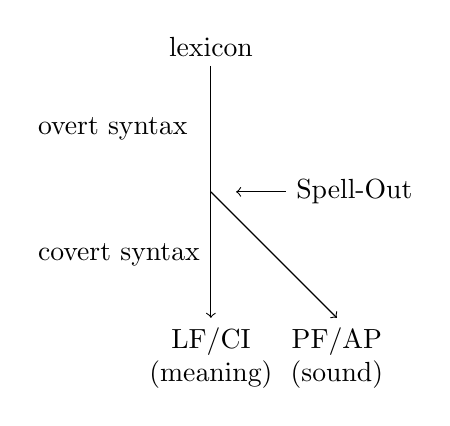
\begin{tikzpicture}[scale=.8]
%\draw (-2.9,-5.8) to[grid with coordinates] (2.7,-0.6);
\draw[->] (0,-1) node[anchor=south] {lexicon} --(0,-5) node[anchor=north, align=center] {LF/CI\\(meaning)};
\draw[->] (0,-3)--(2,-5) node[anchor=north,align=center] {PF/AP\\(sound)};
\draw[<-] (.4,-3)--(1.2,-3) node[anchor=west] {Spell-Out};
%\draw (0,-0.5) node {lexicon};
\draw (-2.9,-2) node[anchor=west] {overt syntax};
\draw (-2.9,-4) node[anchor=west] {covert syntax};
%\draw (0,-6.5) node[align=center] {LF/CI\\(meaning)};
%\draw (2,-5.5) node[align=center] {PF/AP\\(sound)};
\end{tikzpicture}
\caption{\label{fig-architecture-minimalism}Architecture assumed in Minimalist theories before the
  Phase model}
\end{figure}%
Overt syntax stands for syntactic operations that usually have a visible effect. After overt syntax
the syntactic object is sent off to the interfaces and some transformations may take place after
this Spell-Out point. Since such transformations do not affect pronunciation, this part of syntax is
called \emph{covert syntax}. Like in GB's LF, the covert syntax can be used to derive certain scope
readings. 

This architecture was later modified to allow Spell-Out at several points in the derivation. It is now
assumed that there are \emph{phases}\is{phase} in a derivation and that a completed phase is spelled out once it is
used in a combination with a head \citep{Chomsky2008a}. For instance, a subordinated sentence like \emph{that Peter comes} in (\mex{1}) is one
phase and is sent to the interfaces before the whole sentence is completed.\footnote{
  Andreas Pankau (p.\,c.\, 2015) pointed out to me that there is a fundamental problem with such a
  conception of phases, since if it is the case that only elements that are in a relation to a head
  are send off to the interface then the topmost phrase in a derivation would never be sent to the interfaces, since it does not depend on any head.
}

\ea
He believes that Peter comes.
\z
There are different proposals as to what categories form complete phases. Since the concept of
phases is not important for the following introduction, I will ignore this concept in the following. See Section~\ref{sec-dtc} on the psycholinguistic plausibility of phases in
particular and the Minimalist architecture in general. 

\subsection{Valence, feature checking, and agreement}
\label{sec-features-minimalism}

The basic mechanism in Minimalist theories is feature checking.\is{feature!checking} For instance, the noun
\emph{letters} may have a P feature, which means that it has to combine with a PP in order to form a complete phrase.
\ea
letters to Peter
\z
It is assumed that there are interpretable and uninterpretable features. An example of an
interpretable feature is the number feature of nouns. The singular/plural distinction is
semantically relevant. The category features for part of speech information are purely syntactic and
hence cannot be interpreted semantically. Minimalism assumes that all uninterpretable features have
to be used up during the derivation of a complex linguistic object. This process of eating up the
features is called \emph{checking}. As an example, let us consider the noun \emph{letters} again. The
analysis of (\mex{0}) is depicted in Figure~\vref{fig-letters-to-peter-minimalism}.
\begin{figure}
\centering
\begin{forest}
baseline
[N 
  [\emph{letters} {[N, pl, \st{\textit{u}P}]}]
  [P
    [\emph{to} {[P, \st{\textit{u}N}]}]
    [\emph{Peter} {[N]}]]]
\end{forest}
\caption{\label{fig-letters-to-peter-minimalism}Valence representation via uninterpretable features}
\end{figure}%
The fact that the P feature of \emph{letters} is uninterpretable is represented by the little
\emph{u} in front of the P. The uninterpretable P feature of \emph{letters} can be checked against
the P feature of \emph{to Peter}. All checked features are said to delete\is{feature!deletion} automatically. The
deletion is marked by striking the features out in the figures. Strings like (\mex{1}) are ruled out as complete derivations since
the N feature of P is not checked. This situation is shown in Figure~\vref{fig-letters-to-minimalism}.
\ea[*]{
letters to
}
\z
\begin{figure}
\centering
\begin{forest}
baseline
[N 
  [\emph{letters} {[N, pl, \st{\textit{u}P}]}]
  [\emph{to} {[P, \textit{u}N]}]]
\end{forest}
\caption{\label{fig-letters-to-minimalism}Illegitimate syntactic object due to an uninterpretable feature}
\end{figure}%
If this structure would be used in a larger structure that is spelled out, the derivation would
\emph{crash} since the conceptual system could not make sense of the N feature that is still present
at the P node.

%\addlines
Selectional features are atomic, that is, the preposition cannot select an NP[\type{acc}] as in GB
and the other theories in this book unless NP[\type{acc}] is assumed to be atomic. Therefore, an
additional mechanism is assumed that can check other features in addition to selectional
features. This mechanism is called \emph{Agree}\is{Agree|(}.
\eal
\ex[*]{
letters to he
}
\ex[]{
letters to him
}
\zl
The analysis of (\mex{0}b) is shown in Figure~\vref{fig-letters-to-him-minimalism}.
\begin{figure}
\centering
\begin{forest}
baseline
[N 
  [\emph{letters} {[N, pl, \st{\textit{u}P}]}]
  [P
    [\emph{to} {[P, \st{\textit{u}N}, \st{acc}]}]
    [\emph{him} {[N, \st{acc}]}]]]
\end{forest}
\caption{\label{fig-letters-to-him-minimalism}Feature checking via Agree}
\end{figure}%
There is an interesting difference between the checking of selectional features and the checking of
features via Agree. The features that are checked via Agree do not have to be at the top node of the
object that is combined with a head. This will play a role later in the analysis of the passive and
local reordering.%
\is{Agree|)}

\subsection{Phrase structure and \xbart}

The projections of \xbar structures were given in Figure~\ref{Abb-GB-Min-Max} on
page~\pageref{Abb-GB-Min-Max}. According to early versions of the \xbart, there could be arbitrarily
many complements that were combined with \xzero to form an \xbar. Arbitrarily many adjuncts could
attach to \xbar and then at most one specifier could be combined with the \xbar yielding an
XP. Minimalist theories assume binary branching and hence there is at most one
complement, which is the first-merged item. Furthermore, it is not assumed that there is a unique
specifier position. Chomsky rather assumes that all items that are not complements are
specifiers. That is, he distinguishes between first-merged (complements) and later-merged items (specifiers). Figure~\vref{fig-head-comp-spec} shows an example with two specifiers.
\begin{figure}
\centering
\begin{forest}
%where n children=0{}{},
%sm edges
%for tree={parent anchor=south, child anchor=north,align=center,base=bottom}
[XP
  [specifier]
  [\xbar
    [specifier]
    [\xbar
      [complement] [X] ] ] ]
\end{forest}
\caption{\label{fig-head-comp-spec}Complements and specifiers in Minimalist theories}
\end{figure}%
It is also possible to have just a complement and no specifier or to have one or three
specifiers. What structures are ultimately licensed depends on the features of the items that are
involved in the Merge operations. Whether a phrasal projection counts as an \xbar or an XP depends
on whether the phrase is used as a complement or specifier of another head or whether it is used as
head in further Merge operations. If a phrase is used as specifier or complement its status is fixed
to be a phrase (XP), otherwise the projectional status of resulting phrases is left
underspecified. Lexical head daughters in Merge operations have the category X and complex head
daughters in Merge operations have the category \xbar. This solves the problem that standard \xbar
theoretic approaches had with pronouns and proper names: a lot of unary branching structure had to
be assumed (See left picture in Figure~\ref{Abb-GB-Min-Max}). This is not necessary any longer in
current Minimalist theories.\footnote{
  For problems with this approach see \citew[Chapter~2.1]{Brosziewski2003a-u}. 
%% Das ist zu viel hier.
%% It is interesting to
%%   note that these problems do not apply to Categorial Grammar and HPSG, which use techniques for avoiding unary branchings
%%   that are similar to the ones suggested by  
}


\subsection{Little \textit{v}}
\label{sec-little-v}

In\is{category!functional!v@\textit{v}|(} Section~\ref{sec-passive-gb}, I used \xbar structures in which a ditransitive verb was combined
with its accusative object to form a \vbar, which was then combined with the dative object to form a
further \vbar. Such binary branching structures and also flat structures in which both objects are
combined with the verb to form a \vbar are rejected by many practitioners of GB and Minimalism since
the branching does not correspond to branchings that would be desired for phenomena like the binding
of reflexives and negative polarity items. A binding in which \emph{Benjamin} binds \emph{himself}
in (\mex{1}a) is impossible:
\eal
\ex[*]{
Emily showed himself Benjamin in the mirror.
}
\ex[]{
Peter showed himself Benjamin in the mirror.
}
\zl
What is required for the analysis of Binding and NPI phenomena in theories that analyze these
phenomena in terms of tree configurations is that the reflexive pronoun is ``higher'' in the tree than
the proper name \emph{Benjamin}. More precisely, the reflexive pronoun \emph{himself} has to
c-command \emph{Benjamin}. c-command is defined as follows \citep[\page 117]{Adger2003a}:\footnote{
  c-command also plays a prominent role in GB. In fact, one part of Government \& Binding is the
  Binding Theory, which was not discussed in the previous chapter since binding phenomena do not
  play a role in this book.
}
\ea
A node A c-commands B if, and only if A's sister either:\\
\begin{tabular}[t]{@{}l@{~}l@{}}
a. & is B, or\\
b. & contains B
\end{tabular}
\z

In the trees to the left and in the middle of Figure~\vref{fig-ditransitives-options} the c-command
relations are not as desired: in the left-most tree both NPs c-command each other and in the middle
one \emph{Benjamin} c-commands \emph{himself} rather than the other way round.
\begin{figure}
\begin{forest}
baseline
[\vbar
 [\textit{show}]
 [\textit{himself}]
 [\textit{Benjamin}]]
\end{forest}
\hfill
\begin{forest}
baseline
[\vbar
   [\vbar
     [\textit{show}]
     [\textit{himself}] ]
 [\textit{Benjamin}]]
\end{forest}
\hfill\hfill
\begin{forest}
baseline
[\littlevbar
 [\textit{show}]
 [VP
   [\textit{himself}]
   [\vbar
    [V]
    [\textit{Benjamin}]]]]
\end{forest}
\caption{\label{fig-ditransitives-options}Three possible analyses of ditransitives}
\end{figure}%
Hence it is assumed that the structures at the left and in the middle are inappropriate and that
there is some additional structure involving the category \textit{v}, which is called \emph{little v}
\citep[Section~4.4]{Adger2003a}. The sister of \emph{himself} is \vbar and \vbar contains
\emph{Benjamin}, hence \emph{himself} c-commands \emph{Benjamin}. Since the sister of
\emph{Benjamin} is V and V neither is nor contains \emph{himself}, \emph{Benjamin} does not
c-command \emph{himself}. 

The analysis of ditransitives involving an additional verbal head goes back to
\citet{Larson88a}. \citet[\page 70]{HK93a-u} assume that this verbal head contributes a causative
semantics.
%% \todostefan{Andrew McIntyre: the idea of causative light verbs was not used by Larson 1988. (I think
%%   it started in Hale \& Keyser 1993.) Larson also didn't use the term 'little v' (I am not sure, but
%%   I think that term was introduced in Chomsky's black book).} 
The structure in Figure~\ref{fig-ditransitives-little-v} is derived by assuming that the verb \emph{show} starts out
in the V position and then moves to the \textit{v} position. \emph{show} is assumed to mean
\emph{see} and in the position of \littlev it picks up the causative meaning, which results in a
\relation{cause-see} meaning \citep[\page 133]{Adger2003a}. 
\begin{figure}
\centering
\begin{forest}
baseline
[\vP
  [\textit{Peter}]
  [\littlevbar
   [\textit{v} $+$ \textit{show}]
   [VP
     [\textit{himself}]
     [\vbar
      [\phonliste{ show } {[V]}]
      [\textit{Benjamin}]]]]]
\end{forest}
\caption{\label{fig-ditransitives-little-v}Analysis of ditransitives involving movement to \littlev}
\end{figure}%

While the verb shell analysis with an empty verbal head was originally invented by \citet{Larson88a}
for the analysis of ditransitive verbs, it is now also used for the analysis of strictly transitive
and even intransitive verbs.

\citet[Section~4.5]{Adger2003a} argues that semantic roles are assigned uniformly in certain tree
configurations:
\eal
\ex NP daughter of \vP $\to$ interpreted as agent
\ex NP daughter of VP $\to$ interpreted as theme
\ex PP daughter of \littlevbar $\to$ interpreted as goal
\zl
Adger assumes that such uniformly assigned semantic roles help in the process of language
acquisition\is{language acquisition} and from this, it follows that \littlev should also play a role in the analysis of
examples with strictly transitive and intransitive verbs. The
Figures~\ref{fig-transitives-little-v} and~\ref{fig-intransitives-little-v} show the analysis of
sentences containing the verbs \emph{burn} and \emph{laugh}, respectively.\footnote{
  If all intransitive verbs of this type are supposed to have agents as subjects, a very broad
  conception of agent has to be assumed that also subsumes the subject of verbs like
  \emph{sleep}. Usually sleeping is not an activity that is performed intentionally.
}
\begin{figure}
\centering
\begin{forest}
baseline
[\vP
  [Agent]
  [\littlevbar~{[\st{\textit{u}D}]}
   [\textit{v}]
   [VP
      [\textit{burn} {[V, \st{\textit{u}D}]}]
      [Theme]]]]]
\end{forest}
\caption{\label{fig-transitives-little-v}Analysis of strictly transitives involving \littlev}
\end{figure}%

\begin{figure}
\centering
\begin{forest}
baseline
[\vP
  [Agent]
  [\littlevbar~{[\st{\textit{u}D}]}
   [\textit{v} ]
   [ \textit{laugh} {[V]} ]]]
\end{forest}
\caption{\label{fig-intransitives-little-v}Analysis of intransitives involving \littlev}
\end{figure}%
%
\citet[\page 164]{Adger2003a} assumes that intransitive and transitive verbs move from V to \littlev
as well. This will be reflected in the following figures.%
\is{category!functional!v@\textit{v}|)}

\subsection{CP, TP, \vP, VP}
\label{sec-CP-TP-vP-VP}


Section~\ref{sec-GB-CP-IP-System-English} dealt with the CP/IP system in GB. In the course of the
development of Minimalism, the Inflectional Phrase was split into several functional projections \citep{Chomsky89a-u}
% AgrS, TP, Neg, AgrO
of which only the Tense\is{category!functional!Tense} Phrase is assumed in current
Minimalist analyses. So, the TP of Minimalism corresponds to IP in the GB analysis. Apart from this
change, the core ideas of the CP/IP analysis have been transferred to
the Minimalist analysis of English. This subsection will first discuss 
special features that are assumed to trigger movement (Subsection~\ref{sec-epp-features}) and then 
case assignment (Subsection~\ref{sec-case-mp}).




\subsubsection{Features as triggers for movement: The EPP feature on T}
\label{sec-epp-features}


In GB approaches, the modals and auxiliaries were analyzed as members of the
category I and the subjects as specifiers of IP. In the previous section, I showed how subjects are
analyzed as specifiers of \vP. Now, if one assumes that a modal verb combines with such a \vP, the
subject follows the modal, which does not correspond to the order that is observable in English. This
problem is solved by assuming a strong uninterpretable D feature at T. Since the feature is strong,
a suitable D has to move to the specifier of T and check the D
locally. Figure~\vref{fig-Anna-will-read-the-book-minimalism} shows the TP that plays a role in the
analysis of (\mex{1}):
\ea
Anna will read the book.
\z
\begin{figure}
\centering
\begin{forest}
baseline
[TP
 [\textit{Anna} {[D]}]
 [\tbar{[\st{\textit{u}D*}]}
   [\textit{will} T{[pres]}]
   [\vP
     [\phonliste{ Anna }]
     [\littlevbar~{[\st{\textit{u}D}]}
       [\textit{v}
         [\textit{read}] [\textit{v}]]
       [VP
         [\phonliste{ read } {[V, \st{\textit{u}D}]}]
         [DP [\textit{the book}, roof]]]]]]]
\end{forest}
\caption{\label{fig-Anna-will-read-the-book-minimalism}Analysis of \emph{Anna will read the book.}
  involving a modal and movement of the subject from \textit{v} to T}
\end{figure}%
The DP \emph{the book} is the object of \emph{read} and checks the D feature of
\emph{read}. \littlev selects for the subject \emph{Anna}. Since T has a strong D feature (marked by
an asterisk `*'\is{*}), \emph{Anna} must not remain inside of the \vP but moves on to the specifier position of TP.


Full sentences are CPs. For the analysis of (\mex{0}), an empty C head is assumed that is combined
with the TP. The empty C contributes a clause type feature Decl. The full analysis of (\mex{0}) is
shown in Figure~\ref{fig-Anna-will-read-the-book-minimalism-CP}.
\begin{figure}
\centering
\begin{forest}
baseline
[CP
 [C{[Decl]}]
 [TP
 [\textit{Anna} {[D]}]
 [\tbar{[\st{\textit{u}D*}]}
   [\textit{will} T{[pres]}]
   [\vP
     [\phonliste{ Anna }]
     [\littlevbar~{[\st{\textit{u}D}]}
       [\textit{v}
         [\textit{read}] [\textit{v}]]
       [VP
         [\phonliste{ read } {[V, \st{\textit{u}D}]}]
         [DP [\textit{the book}, roof]]]]]]]]
\end{forest}
\caption{\label{fig-Anna-will-read-the-book-minimalism-CP}Analysis of \emph{Anna will read the book.}
  as CP with an empty C with the clause-type feature Decl}
\end{figure}%

%%
%% This is revised later to use an empty wh operator.
%% Too complicated.
%%
%% The analysis of the question in (\mex{1}) involves a strong Q feature for the sentence
%% type question.
%% \ea
%% Will Anna read the newspaper?
%% \z
%% The analysis is shown in Figure~\vref{fig-Will-Anna-read-the-newspaper-minimalism}.
%% \begin{figure}
%% \centering
%% \begin{forest}
%% baseline
%% [CP
%%    [C
%%      [\textit{will} T{[\st{Q*}]}]
%%      [C{[Q]}] ]
%%    [TP
%%    [\textit{Anna} {[D]}]
%%    [\tbar{[\st{\textit{u}D*}]}
%%      [\phonliste{ will } {[T]}]
%%      [\vP
%%        [\phonliste{ Anna }]
%%        [\littlevbar
%%          [\textit{v}]
%%          [VP
%%            [\textit{read} {[V, \textit{u}D]}]
%%            [DP [\textit{the newpaper},roof]]]]]]]]]
%% \end{forest}
%% \caption{\label{fig-Will-Anna-read-the-newspaper-minimalism}Analysis of \emph{Will Anna read the
%%     news paper?}   with an empty C with a strong Q feature for encoding the clause type}
%% \end{figure}%
%% The analysis is parallel to the analysis of the declarative clause except that the modal verb moves
%% to C in order to check the strong Q feature locally.

The analysis of the question in (\mex{1}) involves an unvalued clause-type feature on T for the sentence type
\emph{question}. 
\ea
What will Anna read?
\z
The empty complementizer C has a Q feature that can value the clause-type feature on
T. Since clause-type features on T that have the value Q are stipulated to be strong, the T element
has to move to C to check the feature locally. In addition, the \emph{wh} element is moved. This
movement is enforced by a strong wh feature on C. The analysis of (\mex{0})
is given in Figure~\vref{fig-What-will-Anna-read-minimalism}.
\begin{figure}
\centering
\begin{forest}
baseline
[CP
 [\textit{what} {[D, wh]}]
 [\cbar{[\st{\textit{u}wh*}]}
   [C
     [\textit{will} T{[\st{Q*}]}]
     [C{[Q]}] ]
   [TP
   [\textit{Anna} {[D]}]
   [\tbar{[\st{\textit{u}D*}]}
     [\phonliste{ will } {[T]}]
     [\vP
       [\phonliste{ Anna }]
       [\littlevbar~{[\st{\textit{u}D}]}
         [\textit{v}
           [\textit{read}] [\textit{v}]]
         [VP
           [\phonliste{ read } {[V, \st{\textit{u}D}]}]
           [\phonliste{what}]]]]]]]]
\end{forest}
\caption{\label{fig-What-will-Anna-read-minimalism}Analysis of \emph{What will Anna read?}
  with an empty C with a strong wh feature}
\end{figure}%


%% \ea
%% C > T > (Neg) > (Perf) > (Prog) > (Pass) > \textit{v} > V
%% \z

\subsubsection{Case assignment}
\label{sec-case-mp}

In the GB analysis that was presented in Chapter~\ref{chap-gb}, nominative was assigned by (finite)
I and the other cases by the verb (see Section~\ref{sec-case-assignment}). The assignment of
nominative is taken over to Minimalist analyses, so it is assumed
that nominative is assigned by (finite) T. However, in the Minimalist theory under consideration, there
is not a single verb projection, but there are two verbal projections: \vP and VP. Now, one could
assume that V assigns accusative to its complement or that \textit{v} assigns accusative to the
complement of the verb it dominates. \citet[Section~6.3.2, Section~6.4]{Adger2003a} assumes the latter
approach, since it is compatible with the analysis of so-called unaccusative verbs and the passive. Figure~\vref{fig-Anna-reads-the-book-minimalism-TP} shows the TP for (\mex{1}):
\ea
Anna reads the book.
\z
\begin{figure}
\centering
\begin{forest}
baseline
[TP
 [\textit{Anna} {[D, \st{nom}]}]
 [\tbar{[\st{\textit{u}D*}, \st{nom}]}
   [T{[pres]}]
   [\vP
     [\phonliste{ Anna }]
     [\littlevbar~{[\st{\textit{u}D}]}
       [\textit{v}
         [\textit{read}] [\textit{v} {[\st{acc}]}]]
       [VP
         [\phonliste{ read } {[V, \st{\textit{u}D}]}]
         [DP{[\st{acc}]} [\textit{the book}, roof]]]]]]]
\end{forest}
\caption{\label{fig-Anna-reads-the-book-minimalism-TP}Case assignment by T and \textit{v} in the TP
  for of \emph{Anna reads the book.}}
\end{figure}%
The two NPs \emph{Anna} and \emph{the book} start out with unvalued uninterpretable case features:
[\textit{u}case:].\todostefan{Does read move? Where is the tense feature checked?} The features get
valued by T and \textit{v}. It is assumed that only one feature is checked by Merge, so this would
be the D feature on T, leaving the case feature for the other available checking mechanism:
Agree. Agree can be used to check features in sister nodes, but also features further away in the
tree. The places that are possible candidates for Agree relations have to stand in a certain
relation to each other. The first node has to c-command the node it Agrees with. c-command roughly
means: one node up and then arbitrarily many nodes down. So \textit{v} c-commands VP, V, the DP
\emph{the book}, and all the nodes within this DP. Since Agree can value features of c-commanded
nodes, the accusative on \textit{v} can value the case feature of the DP \emph{the book}.

The non-locality that is build into Agree raises a problem: why is it that (\mex{1}) is
ungrammatical?
\ea[*]{
\label{ex-him-likes-she}
Him likes she.
}
\z
The accusative of \textit{v} could be checked with its subject and the nominative of T with the
object of \emph{likes}. Both DPs stand in the necessary c-command relations to T and \textit{v}. This
problem is solved by requiring that all Agree relations have to involve the closest possible
element. \citet[\page 218]{Adger2003a} formulates this constraint as follows:
\ea
\label{principle-locality-of-matching}
Locality of matching\is{locality!of matching}: Agree holds between a feature F on X and a matching feature F on Y if and only
if there is no intervening Z[F].
\z
Intervention is defined as in (\mex{1}):\todostefan{Fritz Hamm: Da fehlt die Hälfte: eine zweite
  c-commando Beziehung}
\ea
\label{def-intervention}
Intervention\is{intervention}: In a structure [X \ldots{} Z \ldots{} Y], Z intervenes between X and Y iff X
c-commands\is{c"=command} Z and Z c-commands Y.
\z

So, since T may Agree with \emph{Anna} it must not Agree with \emph{the book}. Hence
nominative assignment to \emph{she} in (\ref{ex-him-likes-she}) is impossible and (\ref{ex-him-likes-she}) is correctly ruled out.

\subsection{Adjuncts}

\citet[Section~4.2.3]{Adger2003a} assumes that adjuncts attach to XP and form a new XP. He calls
this operation \emph{Adjoin}. Since this operation does not consume any features it is different from
External Merge and hence a new operation would be introduced into the theory, contradicting
Chomsky's claim that human languages use only Merge as a structure building operation. There are
proposals to treat adjuncts as elements in special adverbial phrases with empty heads (see
Section~\ref{sec-functional-projections-minimalism}) that are also assumed to be part of a hierarchy of functional
projections. Personally, I prefer Adger's solution that corresponds to what is done in many other
frameworks: there is a special rule or operation for the combination of adjuncts and heads (see for instance
Section~\ref{sec-adjuncts-hpsg} on the HPSG schema for head adjunct combinations).


\section{Verb position}
\label{sec-verb-position-MP}

The analysis of verb first sentences in German is straightforward, given the machinery that was
introduced in the previous section. The basic idea is the same as in GB: the finite verb moves from V to
\textit{v} to T and then to C. The movement to T is forced by a strong tense feature on T and the movement of
the T complex to C is enforced by a clause-type feature on T that is valued as a strong Decl by C. The analysis of (\mex{1}) is shown in
Figure~\vref{fig-kennt-jeder-diesen-mann-minimalism}.
\ea
\gll Kennt jeder diesen Mann?\\
     knows everybody this man\\
\glt `Does everybody know this man?'
\z
\begin{figure}
\begin{forest}
[CP
    [C
      [T{[\st{Decl*}]}
        [\textit{kennt} {[\st{Pres*}]}]
        [T{[Pres]}]]
      [C{[Decl]}]]
    [TP
      [\textit{jeder}]
      [\tbar{[\st{\textit{u}D*}]}
        [\vP
          [\phonliste{ jeder }]
          [\littlevbar
            [VP
              [DP [\textit{diesen Mann}, roof] ]
              [\phonliste{ kennt }]]
            [\textit{v}
              [\phonliste{ kennt }]
              [\textit{v}]]]]
        [\phonliste{ kennt T }]]]]
\end{forest}
\caption{\label{fig-kennt-jeder-diesen-mann-minimalism}Analysis of \emph{Kennt jeder diesen Mann?} `Does everybody know this man?' following the
  analysis of \citet{Adger2003a}}
\end{figure}%


\section{Long"=distance dependencies}

Having explained the placement of the verb in initial position, the analysis of V2 sentences does
not come with a surprise: \citet[\page 331]{Adger2003a} assumes a feature that triggers the movement
of a constituent to a specifier position of C. Adger calls this feature top, but this is a misnomer
since the initial position in German declarative sentences is not restricted to topics. Figure~\vref{fig-diesen-mann-kennt-jeder}
shows the analysis of (\mex{1}):
\ea
\gll Diesen Mann kennt jeder.\\
     this man    knows everybody\\
\glt `Everbody knows this man.'
\z
\begin{figure}
\begin{forest}
[CP
  [\emph{diesen Mann} {[top] }]
  [\cbar{[\st{\textit{u}top*}]}
    [C
      [T{[\st{Decl*}]}
        [\textit{kennt} {[\st{Pres*}]}]
        [T{[Pres]}]]
      [C{[Decl]}]]
    [TP
      [\textit{jeder}]
      [\tbar{[\st{\textit{u}D*}]}
        [\vP
          [\phonliste{ jeder }]
          [\littlevbar
            [VP
              [\phonliste{ diesen Mann }{[D]}]
              [\phonliste{ kennt }]]
            [\textit{v}
              [\phonliste{ kennt }]
              [\textit{v}]]]]
        [\phonliste{ kennt T }]]]]]
\end{forest}
\caption{\label{fig-diesen-mann-kennt-jeder}Analysis of \emph{Diesen Mann kennt jeder.} `This man, everybody knows.' following the
  analysis of \citet[\page 331]{Adger2003a}}

\end{figure}%


\section{Passive}

\citet{Adger2003a}\is{passive|(} suggests an analysis for the passive in English, which I adapted here to
German.\todostefan{Add example with movement to T according to Adger} Like in the GB analysis that was discussed in Section~\ref{sec-passive-gb} it is assumed
that the verb does not assign accusative to the object of \emph{schlagen} `to beat'. In Minimalist terms, this
means that \littlev does not have an acc feature that has to be checked. This special version of
\littlev is assumed to play a role in the analysis of sentences of so-called unaccusative
verbs \citep{Perlmutter78}. Unaccusative verbs\is{verb!unaccusative} are a subclass of intransitive verbs that have many interesting
properties. For instance, they can be used as adjectival participles\is{participle!adjectival} although this is usually not
possible with intransitive verbs:
\eal
\ex[*]{
\gll der getanzte Mann\\
     the danced man\\
}
\ex[]{
\gll der gestorbene Mann\\
     the died man\\
\glt `the dead man'
}
\zl
The explanation of this difference is that adjectival participles predicate over what is the object
in active sentences:
\eal
\ex
\gll dass der Mann das Buch gelesen hat\\
     that the man  the book read has\\
\glt `that the man read the book'
\ex
\gll das gelesene Buch\\
     the read book\\
\zl
Now the assumption is that the argument of \emph{gestorben} `died' behaves like an object, while the
argument of \emph{getanzt} `danced' behaves like a subject. If adjectival passives predicate over the object
it is explained why (\mex{-1}b) is possible, while (\mex{-1}a) is not. 

%\addlines[2]
\citet[\page 140]{Adger2003a} assumes the structure in Figure~\vref{fig-little-v-unaccusative} for \vPs with unaccusative verbs.
\begin{figure}
\begin{forest}
[\vP
  [\textit{v}]
  [VP
    [\textit{fall}{[V, \textit{u}N]}]
    [Theme]]]
\end{forest}
\caption{\label{fig-little-v-unaccusative}Structure of \vP with unaccusative verbs like \emph{fall},
  \emph{collapse}, \emph{wilt} according to \citet[\page 140]{Adger2003a}}
\end{figure}%
It is assumed that this unaccusative variant of \littlev plays a role in the analysis of the
passive. Unaccusative verbs are similar to passivized verbs in that they do have a subject that
somehow also has object properties. The special version of \littlev is selected by the Passive head
\emph{werden} `be', which forms a Passive Phrase\is{category!functional!Passive} (abbreviated as
PassP). See Figure~\ref{fig-passive-schlagen-mp} for the analysis of the example in (\mex{1}):
\ea
\gll dass er geschlagen wurde\\
     that he beaten was\\
\glt `that he was beaten'
\z
\begin{figure}
\centerfit{
%\begin{sideways}  
\begin{forest}
for tree={fit=rectangle}
[TP
     [PassP
       [\vP
         [VP
           [pronoun {[\st{nom}]} ]
           [\phonliste{schlagen}]]
         [\textit{v}
           [\textit{schlagen}]
           [{\textit{v}[\st{\textit{u}Infl}:Pass]}]]]
       [\phonliste{werden}]]
     [{T[past,\st{nom}]}
       [\textit{werden} {[Pass,\st{\textit{u}Infl}:past*]}]
       [{T[past]}]]]
\end{forest}
%\end{sideways}
}
\caption{\label{fig-passive-schlagen-mp}Minimalist analysis of the passive without movement but with
nonlocal case assignment via Agree}
\end{figure}%
The Pass head requires the Infl feature of \littlev to have the value Pass, which results in participle morphology at
spellout. Hence the form that is used is \emph{geschlagen} `beaten'. The auxiliary moves to T to check the
strong Infl feature at T and since the Infl feature is past, the past form of \emph{werden} `be', namely
\emph{wurde} `was', is used at spellout. T has a nom feature that has to be checked. Interestingly, the
Minimalist approach does not require the object of \emph{schlagen} to move to the specifier position
of T in order to assign case, since case assignment is done via Agree. Hence in principle, the pronominal argument
of \emph{schlagen} could stay in its object position and nevertheless get nominative
from T. This would solve the problem of the GB analysis that was pointed out by \citet[Section~4.4.3]{Lenerz77}. See
page~\pageref{ex-passive-German-no-movement} for Lenerz' examples and discussion of the
problem.\todostefan{Check Schäfer and Alexiadou}
However, \citet[\page 332]{Adger2003a} assumes that German has a strong EPP feature on T. If this
assumption is upheld, all problems of the GB account will carry over to the Minimalist analysis: all
objects have to move to T even when there is no reordering taking place. Furthermore, impersonal
passives of the kind in (\mex{1}) would be problematic, since there is no noun phrase that could be
moved to T in order to check the EPP feature:
\ea
\gll weil getanzt wurde\\
     because danced was\\
\glt `because there was dancing there'
\z
\is{passive|)}

\section{Local reordering}

\citet{Adger2003a} does not treat local reordering. But there are several other suggestions in the
literature. Since all reorderings in Minimalist theories are feature-driven, there must be an item
that has a feature that triggers reorderings like those in (\mex{1}b):
\eal
\ex 
\gll {}[weil] jeder diesen Mann kennt\\
	 {}\spacebr{}because everyone this man knows\\
\glt `because everyone knows this man'
\ex 
\gll {}[weil] diesen Mann jeder kennt\\
	 {}\spacebr{}because this man everyone knows\\
\zl
There have been various suggestions involving functional projections like Topic Phrase \citep[\page 222]{Laenzlinger2004a} or AgrS and
AgrO \citep[Chapter~4]{Meinunger2000a} that offer places to move to. G.\ \citet[Section~3.5]{GMueller2014a-u} offers a leaner solution, though. In his approach, the
object simply moves to a second specifier position of \littlev. The analysis is depicted in
Figure~\vref{fig-scrambling-minimalism}.\footnote{
  G.\,Müller assumes optional features on \textit{v} and V that trigger local reorderings (p.\,48). These are not
  given in the figure.
} 

\begin{figure}
\begin{forest}
[CP
    [C
      [dass]]
    [TP
        [\vP
          [\emph{diesen Mann}]
          [\littlevbar
            [ \emph{jeder}]
            [\littlevbar
                [VP
                  [\phonliste{ diesen Mann } {[D]}] 
                  [\phonliste{ kennt }]]
                [\textit{v}
                  [\phonliste{ kennt }]
                  [\textit{v}]]]] ]
        [\textit{kennt} {[T]}]]]
\end{forest}
\caption{\label{fig-scrambling-minimalism}Analysis of \emph{dass diesen Mann jeder kennt} `that everybody knows this man' as movement
  of the object to a specifier position of \textit{v}}
\end{figure}%

An option that was suggested by \citet[\page 229--230]{Laenzlinger2004a} is to assume several Object
Phrases for objects that may appear in any order. The objects move to the specifier positions of
these projections and since the order of the Object Phrases is not restricted, both orders in
(\mex{1}) can be analyzed:
\eal
\ex 
\gll dass Hans diesen Brief meinem Onkel gibt\\
     that Hans this letter my uncle gives\\
\glt `that Hans gives this letter to my uncle'
\ex
\gll dass Hans meinem Onkel diesen Brief gibt\\
     that Hans my uncle this letter gives\\
\glt `that Hans gives to my uncle this letter'
\zl

%\if 0
\section{New developments and theoretical variants}
\label{Abschnitt-neues-GB}


At the start of the 90s, Chomsky suggested a major rethink of the basic theoretical assumptions of GB and only keeping
those parts of the theory which are absolutely necessary. In the \emph{Minimalist Program}, Chomsky gives the central motivations for the far"=reaching
revisions of GB theory \citep{Chomsky93b-u,Chomsky95a-u}. Until the beginning of the 90s, it was
assumed that Case Theory\is{Case Theory}, the Theta"=Criterion\is{theta-criterion@Theta"=Criterion}, \xbart, Subjacency\is{Subjacency}, Binding
Theory\is{Binding Theory}, Control Theory\is{Control Theory} etc.\ all belonged to the innate faculty
for language \citep[\page 804]{Richards2015a}. This, of 
courses, begs the question of how this very specific linguistic knowledge made its way into our genome. The Minimalist Program follows up on this
point and attempts to explain properties of language through more general cognitive principles and to reduce the amount of innate language"=specific 
knowledge postulated. The distinction between Deep Structure and Surface Structure\is{D"=structure}\is{S"=structure}, for example, was abandoned.
Move still exists as an operation, but can be used directly to build sub"=structures rather than after a complete D"=structure has been created.
Languages differ with regard to whether this movement is visible or not.

Although Chomsky's Minimalist Program should be viewed as a successor to GB, advocates of Minimalism often emphasize the fact that Minimalism is not
a theory as such, but rather a research program (Chomsky \citeyear[\page 4]{Chomsky2007a};
\citeyear[\page 6]{Chomsky2013a}). The actual analyses suggested by \citet{Chomsky95a-u} when introducing the research program have been reviewed by theoreticians and have sometimes come in for serious criticism
\citep*{Kolb97a,JL97a-u-platte,JL99a-u-gekauft,LLJ2000b,LLJ2000a,LLJ2001a,Seuren2004a,PJ2005a},
however, one should say that some criticisms overshoot the mark.

There are various strains of Minimalism. In the following sections, I will discuss some of the
central ideas and explain which aspects are regarded problematic.

\subsection{Move, Merge, feature"=driven movement and functional projections}
\label{Abschnitt-merkmalsgetriebene-Bewegung}
\label{Abschnitt-MP-funktionale-Projektionen}\label{sec-functional-projections-minimalism}
\label{Abschnitt-Kaynesche-Modelle}

Johnson, Lappin and Kolb have criticized the computational aspects of Chomsky's system. Chomsky suggested incorporating principles of economy into
the theory. In certain cases, the grammatical system can create an arbitrary number of structures, but only the most economical, that is, the one which
requires the least effort to produce, will be accepted as grammatical (transderivational economy\is{economy!transderivational}). This assumption
does not necessarily have to be taken too seriously and, in reality, does not play a role in many works in the Minimalist framework (although see
\citet{Richards2015a} for recent approaches with derivations which are compared in terms of economy). Nevertheless, there are other aspects of 
Chomsky's theory which can be found in many recent works. For example, Chomsky has proposed reducing
the number of basic, structure building operations which license structures to two: Move\is{Move} and Merge\is{Merge} (that is, Internal\is{Merge!Internal} and External\is{Merge!External} Merge).
Move corresponds to the operation \movea, which was already discussed in Chapter~\ref{chap-gb}, and
Merge is the combination of (two) linguistic objects.

%\addlines[2]
It is generally assumed that exactly two objects can be combined \citep[\page 226]{Chomsky95a-u}.
For Move, it is assumed that there must be a reason for a given movement operation. The reason for
movement is assumed to be that an element can check some feature\is{feature checking} in the position it is moved to. This idea was already presented in the analysis of the passive in
Section~\ref{Abschnitt-GB-Passiv}: the accusative object does not bear case in passive sentences and therefore has to be moved to a position
where it can receive case. This kind of approach is also used in newer analyses for a range of other phenomena. For example, it is assumed that
there are phrases whose heads have the categories focus\is{focus} and topic\is{topic}. The
corresponding functional heads are always empty in languages like German and English.
Nevertheless, the assumption of these heads is motivated by the fact that other languages possess
markers which signal the topic or focus of a sentence morphologically. This argumentation is only
possible if one also assumes that the inventory of categories is the same for all languages. Then,
the existence of a category in one language would suggest the existence of the same category in all
other languages. This assumption of a shared universal component (Universal Grammar, UG)\indexug
with detailed language"=specific knowledge is, however, controversial and is shared by few linguists
outside of the Chomskyan tradition. Even for those working in Chomskyan linguistics, there have been
questions raised about whether it is permissible to argue in this way since if it is only the ability to create recursive structures that is responsible for the
human-specific ability to use language (faculty of language in the narrow sense) -- as \citet*{HCF2002a}
assume --, then the individual syntactic categories are not part of UG and data from other languages cannot be used
to motivate the assumption of invisible categories in another language.

\subsubsection{Functional projections and modularization of linguistic knowledge}

The assumption that movement must be licensed by feature checking has led to an inflation of the number of (silent) functional 
heads\is{category!functional}.\footnote{
	The assumption of such heads is not necessary since features can be 'bundled' and then they
        can be checked together. For an approach in this vein,
	which is in essence similar to what theories such as HPSG\indexhpsg assume, see \citew[Section~II.3.3.4,
  Section~II.4.2]{Sternefeld2006a-u}.

In so"=called cartographic\is{cartography} approaches, it is assumed that every morphosyntactic feature corresponds to an independent syntactic
head \citep[\page 54, 61]{CR2010a}. For an explicitly formalized proposal in which exactly one
feature is consumed during a combination operation see \citew[\page 335]{Stabler2001a}. Stabler's \emph{Minimalist
    Grammars}\indexmg are discussed in more detail in Section~\ref{Abschnitt-MG}.
} 
\citet[\page 297]{Rizzi97a-u} suggests the structure in Figure~\vref{Abbildung-Rizzi} (see also Grewendorf \citeyear[\page 85, 240]{Grewendorf2002a}; \citeyear{Grewendorf2009a}).\pagebreak

\begin{figure}
\centering
\newlength\mytextheight
\settototalheight{\mytextheight}{XpX$^0$X$'$}
\begin{forest}
  delay={
    where content={}{
      content={\phantom{X}}
    }{},
  },
  for tree={
    text height=\mytextheight,
    fit=band,
    parent anchor=south,
    child anchor=north,
  }
[ForceP
	[]
	[Force$'$
		[Force$^0$]
		[TopP*
			[]
			[Top$'$
				[Top$^0$]
				[FocP
					[]
					[Foc$'$
						[Foc$^0$]
						[TopP*
							[]
							[Top$'$
								[Top$^0$]
								[FinP
									[]
									[Fin$'$
										[Fin$^0$]
										[IP]]]]]]]]]]]
\end{forest}

\caption{\label{Abbildung-Rizzi}Syntactic structure of sentences following \citet[\page 297]{Rizzi97a-u}}
\end{figure}%
The functional categories Force\is{category!functional!Force}, Top\is{category!functional!Top}, Foc\is{category!functional!Foc} and
Fin\is{category!functional!Fin} correspond to clause type, topic, focus and finiteness. It is assumed that movement always targets a specifier
position. Topics and focused elements are always moved to the specifier position of the corresponding phrase. Topics can precede or follow focused
elements, which is why there are two topic projections: one above and one below FocP. Topic phrases
are recursive, that is, an arbitrary number of TopPs can appear at the positions of TopP in the figure. Following \citet[\page
  70]{Grewendorf2002a}, topic and focus phrases are only realized if they are required for particular information structural reasons, such as 
movement.\footnote{
	There are differing opinions as to whether functional projections are optional or not. Some
        authors assume that the complete hierarchy of functional projections is always present but functional heads can remain empty (\eg \citealp[\page 106]{Cinque99a-u} and \citealp[\page 55]{CR2010a}).
}
\citet[\page 147]{Chomsky95a-u}\label{Seite-AgrO} follows \citet{Pollock89a-u} 
in assuming that all languages have functional projections for subject and object agreement\is{agreement!object} as well as negation
(AgrS\is{category!functional!AgrS}, AgrO\is{category!functional!AgrO},
Neg\is{category!functional!Neg}).\footnote{
	See \citew[Section~4.10.1]{Chomsky95a-u}, however.
}
\citet[\page 78]{Sternefeld95a}, \citet[\page 103]{Stechow96a} and \citet[\page 100--101, 124]{Meinunger2000a}
differentiate between two agreement positions for direct and indirect objects (AgrO\is{category!functional!AgrO},
AgrIO\is{category!functional!AgrIO}). As well as AgrS\is{category!functional!AgrS}, AgrO\is{category!functional!AgrO} 
and Neg\is{category!functional!Neg}, \citet{BS97a-u} assume the functional heads Share\is{category!functional!Share} and 
Dist\is{category!functional!Dist} in order to explain scope phenomena in English as feature"=driven movements at LF. For a treatment
of scope phenomena without empty elements or movement, see Section~\ref{Abschnitt-leere-Elemente-Semantik}.  
\citew[\page 13]{BG2005a} assume the categories $-$PolP\is{category!functional!$-$Pol}, $+$PolP\is{category!functional!+Pol} and
\%PolP\is{category!functional!\%Pol} for their discussion of polarity.

\citet[\page 76]{Webelhuth95a} gives an overview of the functional projections that had been proposed up to 1995 and offers references for AgrA\is{category!functional!AgrA},
AgrN\is{category!functional!AgrN}, AgrV\is{category!functional!AgrV},
Aux\is{category!functional!Aux}, Clitic Voices\is{category!functional!Clitic Voices}, Gender\is{category!functional!Gender},
Honorific\is{category!functional!Honorific}, $\mu$\is{category!functional!$\mu$}, Number\is{category!functional!Number}, Person\is{category!functional!Person}, 
Predicate\is{category!functional!Predicate}, Tense\is{category!functional!Tense}, Z\is{category!functional!Z}.

In addition to AdvP\is{category!functional!Adverb}, NegP\is{category!functional!Neg}, AgrP, FinP,
TopP and ForceP, \citet*{WHBH2007a-u} postulate an OuterTopP\is{category!functional!OuterTop}. 
%
\citet[\page 31]{Poletto2000a-u} suggests both a HearerP\is{category!functional!Hearer} and a SpeakerP\is{category!functional!Speaker} for the 
position of clitics in Italian\il{Italian}.
%
\citet[\page 75]{BB2011a-u} assume a BenefactiveP\is{category!functional!Benefactive}

\addlines
\citet[\page 106]{Cinque99a-u} adopts the 32 functional heads in Table~\vref{Tabelle-Cinque} in his work.
\begin{table}
\begin{tabular}[t]{@{}r@{~~}l@{~~~}r@{~~}l@{~~~}r@{~~}l@{~~~}r@{~~}l@{}}
\lsptoprule
 1. & Mood\sub{Speech Act}     &  2. & Mood\sub{Evaluative}     &  3. & Mood\sub{Evidential}      &  4. & Mood\sub{Epistemic}\\
 5. & T(Past)                  &  6. & T(Future)                &  7. & Mood\sub{Irrealis}        &  8. & Mod\sub{Necessity}\\
 9. & Mod\sub{Possibility}     & 10. & Mod\sub{Volitional}      & 11. & Mod\sub{Obligation}       & 12. & Mod\sub{Ability/permission}\\
13. & Asp\sub{Habitual}        & 14. & Asp\sub{Repetitive(I)}   & 15. & Asp\sub{Frequentative(I)} & 16. & Asp \sub{Celerative(I)}\\
17. & T(Anterior)              & 18. & Asp\sub{Terminative}     & 19. & Asp\sub{Continuative}     & 20. & Asp\sub{Perfect(?)}\\
21. & Asp\sub{Retrospective}   & 22. & Asp\sub{Proximative}     & 23. & Asp\sub{Durative}         & 24. & Asp\sub{Generic/progressive}\\
25. & Asp\sub{Prospective}     & 26. & Asp\sub{SgCompletive(I)} & 27. & Asp\sub{PlCompletive}     & 28. & Asp\sub{Voice}\is{category!functional!Voice}\\
29. & Asp \sub{Celerative(II)} & 30. & Asp\sub{SgCompletive(II)}& 31. & Asp\sub{Repetitive(II)}   & 32. & Asp\sub{Frequentative(II)}\\
\lspbottomrule
\end{tabular}
\is{category!functional!Mood}\is{category!functional!T}\is{category!functional!Mod}\is{category!functional!Asp}\is{category!functional!Perfect(?)}%
\caption{\label{Tabelle-Cinque}Functional heads following \citew[\page 106]{Cinque99a-u}}
\end{table}%
He assumes that all sentences contain a structure with all these functional heads. The specifier positions of these heads can be occupied by adverbs
or remain empty. Cinque claims that these functional heads and the corresponding structures form part of Universal Grammar\indexug, that is, 
knowledge of these structures is innate (page~107).\footnote{
	Table~\ref{Tabelle-Cinque} shows only the functional heads in the clausal
        domain. \citet[\page 96, 99]{Cinque94a-u} also accounts for the order of 
	adjectives with a cascade of projections:
	Quality\is{category!functional!Quality}, Size\is{category!functional!Size},
  Shape\is{category!functional!Shape}, Color\is{category!functional!Color},
  Nationality\is{category!functional!Nationality}.
  These categories and their ordering are also assumed to belong to UG (p.\,100). 

  \citet[\page 96]{Cinque94a-u} claims that a maximum of seven attributive adjectives are possible and explains this
  with the fact that there are a limited number of functional projections in the nominal domain. As was shown on page~\pageref{Beispiel-Iteration-Adjektive},
  with a fitting context it is possible to use several adjectives of the same kind, which is why some of Cinque's functional projections would have
  to be subject to iteration.
}
\citet{Laenzlinger2004a} follows Cinque in proposing this sequence of functional heads for German. He also follows \citet{Kayne94a-u}, who assumes
that all syntactic structures have the order specifier head complement cross"=linguistically, even if the surface order of the constituents
seems to contradict this.%\pagebreak

The constituent orders that are visible in the end are derived by leftward"=movement.\footnote{\label{fn-Kayne-Extraposition}%
	This also counts for extraposition\is{extraposition}, that is, the movement of constituents into the postfield
	in German. Whereas this would normally be analyzed as rightward"=movement, \citet[Chapter~9]{Kayne94a-u} analyzes
	it as movement of everything else to the left. Kayne assumes that (i.b) is derived from (i.a) by moving part of the 
	NP:
\eal
\ex just walked into the room [\sub{NP} someone who we don't know].
\ex Someone$_i$ just walked into the room [\sub{NP} \_$_i$ who we don't know].
\zl
(i.a) must have to be some kind of derived intermediate representation, otherwise English would not be SV(O) underlyingly but rather V(O)S.
(i.a) is therefore derived from (ii) by fronting the VP \emph{just walked into the room}.
\ea
Someone who we don't know just walked into the room
\z
Such analyses have the downside that they cannot be easily combined with performance models (see Chapter~\ref{Abschnitt-Diskussion-Performanz}).%
} 
Figure~\vref{Abbildung-Remnant-Movement-Satzstruktur} shows the analysis of a verb"=final clause where the functional adverbial heads have been
omitted.\footnote{
	These structures do not correspond to \xbar theory as it was presented in Section~\ref{sec-xbar}. In some cases, heads have been combined
	with complements to form an XP rather than an X$'$. For more on \xbar theory in the Minimalist Program, 
	see Section~\ref{Abschnitt-Spezfikatoren-MP}.
}
%%\begin{figure}
%\resizebox{\linewidth}{!}
%%\centerline{
%\small
%% \psset{xunit=7.5mm,yunit=6mm}
%% %
%% \begin{pspicture}(-0.4,4)(14.2,20.2)
%% \rput[B](2,20){\rnode{ForceP}{CP}}
%% \rput[B](0,18){\rnode{C}{\cnull}}
%% \rput[B](4,18){\rnode{ForceS}{SubjP}}
%% \rput[B](2,16){\rnode{Force}{DP}}
%% \rput[B](6,16){\rnode{TopP}{\ldots ObjP}}
%% \rput[B](4,14){\rnode{SpecTopP}{DP}}
%% \rput[B](8,14){\rnode{TopS}{\ldots AuxP}}
%% \rput[B](6,12){\rnode{SpecAuxP}{VP}}
%% \rput[B](10,12){\rnode{FocP}{Aux+}}
%% \rput[B](8,10){\rnode{Aux}{Aux}}
%% \rput[B](12,10){\rnode{FocS}{\ldots VP}}
%% \rput[B](10,8){\rnode{Foc}{V}}
%% \rput[B](14,8){\rnode{TopP2}{DP}}
%% %
%% \psset{angleA=-90,angleB=90,arm=0pt}
%% %
%% \ncdiag{ForceP}{C}\ncdiag{ForceP}{ForceS}
%% \ncdiag{ForceS}{Force}\ncdiag{ForceS}{TopP}
%% \ncdiag{TopP}{SpecTopP}\ncdiag{TopP}{TopS}
%% \ncdiag{TopS}{SpecAuxP}\ncdiag{TopS}{FocP}
%% \ncdiag{FocP}{Aux}\ncdiag{FocP}{FocS}
%% \ncdiag{FocS}{Foc}\ncdiag{FocS}{TopP2}
%% \ncdiag{TopP2}{SpecTopP2}\ncdiag{TopP2}{TopS2}
%% \ncdiag{TopS2}{Top2}\ncdiag{TopS2}{FinP}
%% \ncdiag{FinP}{SpecFinP}\ncdiag{FinP}{FinS}
%% \ncdiag{FinS}{Fin}\ncdiag{FinS}{IP}
%% %
%% %\psgrid
%% %
%% \rput[B](0,6){\rnode{weil}{weil}}
%% \rput[B](2,6){\rnode{Mann}{der Mann}}
%% \rput[B](4,6){\rnode{Buch}{das Buch}}
%% \rput[B](6,6){\rnode{gelesen}{gelesen}}
%% \rput[B](8,6){\rnode{hat}{hat}}
%% %
%% \ncdiag{C}{weil}
%% \ncdiag{SpecAuxP}{gelesen}
%% \ncdiag{Aux}{hat}
%% \pstriangle(2,6.7)(1.6,9)
%% \pstriangle(4,6.7)(1.6,7)
%% \pscircle(12,8.5){1.9}
%% \psline{->}(12,5.4)(12,5)(6,5)(6,5.6)
%% \psline{->}(14,7.8)(14,4)(4,4)(4,5.6)
%% \end{pspicture}}
%% \caption{\label{Abbildung-Remnant-Movement-Satzstruktur}Analyse der Satzstruktur mit Restbewegung nach links}
%% \end{figure}%
\begin{figure}
\oneline{%
\begin{forest}
where n children=0{delay=with translation}{}
[CP
	[C$^0$[weil;because, tier=word]]
	[TopP
		[DP$_j$ [diese Sonate;this sonata,tier=below,l=31\baselineskip]]
		[SubjP
			[DP$_i$ [der Mann;the man,tier=word]]
			[ModP
				[AdvP [wahrscheinlich;probably,l=20\baselineskip]]
				[ObjP
					[DP$_j$ [diese Sonate;this sonata,tier=below]]
					[NegP
						[AdvP [nicht;not,tier=word]]
						[AspP
							[AdvP [oft;often,tier=word]]
							[MannP
								[AdvP [gut;well,tier=word]]
								[AuxP
									[VP$_k$ [gespielt;played,tier=word]]
									[Aux+
										[Aux [hat;has,tier=word]]
										[vP
											[DP$_i$]
											[VP$_k$
												[V]
												[DP$_j$
                                                                                                  [,phantom,tier=word]]]]]]]]]]]]]]
\end{forest}%
}
\caption{\label{Abbildung-Remnant-Movement-Satzstruktur}Analysis of sentence structure with leftward remnant movement
  and functional heads following \citet[\page 224]{Laenzlinger2004a}}
\end{figure}%
Subjects and objects are generated as arguments inside of vP and VP, respectively. The subject is moved to the specifier of the subject phrase\is{category!functional!Subj}
and the object is moved to the specifier of the object phrase\is{category!functional!Obj}. The verbal projection (VP$_k$) is moved in front of
the auxiliary into the specifier position of the phrase containing the auxiliary. The only function of SubjP and ObjP is to provide a landing site
for the respective movements. For a sentence in which the object precedes the subject, Laenzlinger assumes that the object moves to the specifier of a topic
phrase. Figure~\ref{Abbildung-Remnant-Movement-Satzstruktur} contains only a ModP and an AspP, although Laenzlinger assumes that all the heads proposed by Cinque are present
in the structure of all German clauses. For ditransitive verbs, Laenzlinger assumes multiple object
phrases (page~230). A similar analysis with movement of object and subject from verb"=initial VPs to
Agr positions was suggested by \citet{Zwart1994a-u} for Dutch\il{Dutch}.


For general criticism of Kayne's model, see \citew{Haider2000a}. Haider shows that a Kayne"=like
theory makes incorrect predictions for German (for instance regarding the position of selected
adverbials and secondary predicates and regarding verbal complex formation) and therefore fails to live up to its billing as a theory which
can explain all languages. \citet[Section~4]{Haider97a} has shown that the assumption of an empty Neg\is{category!functional!Neg} head,
as assumed by \citet{Pollock89a-u}, \citet{Haegeman95a-u} and others, leads to problems. See
\citew{Bobaljik99a} for problems with the argumentation for Cinque's cascade of adverb"=projections.

Furthermore, it has to be pointed out that SubjP and ObjP, TraP\is{category!functional!Tra} (Transitive
Phrase) and IntraP\is{category!functional!Intra} (Intransitive Phrase) (\citealp[\page 1745]{Karimi-Doostan2005a}) and
TopP\is{category!functional!Top} (topic phrase), DistP\is{category!functional!Dist}\linebreak (quantifier
phrase), AspP\is{category!functional!Asp} (aspect phrase) (\citealp[\page 22]{EKiss2003a-u}; \citealp[\page
35]{Karimi2005a}), PathP\is{category!functional!PathP} and PlaceP\is{category!functional!PlaceP}
\citep[\page 246]{Svenonius2004a-u} encode information about grammatical function\is{grammatical function}, valence,
information structure and semantics in the category symbols.\footnote{
	For further examples and references, see Newmeyer (\citeyear[\page 194]{Newmeyer2004b};
  \citeyear[\page 82]{Newmeyer2005a}). Newmeyer references also works which stipulate a projection
  for each semantic role, \eg Agent, Reciprocal, Benefactive, Instrumental, Causative,
  Comitative, and Reversive Phrase.
}
%
%% \ifdraft
%% \begin{table}
%% %\renewcommand{\tabularxcolumn}[1]{m{#1}}
%% %\newcolumntype{Y}{>{\raggedright\arraybackslash}X}
%% \begin{tabular}{|l|p{40mm}|p{43mm}|}\hline
%%                      & functionalr Kopf                      & Quelle\\\hline
%% Valenz               & IntraP (Intransitive Phrase)           & \citew[\page 1745]{Karimi-Doostan2005a}           \\
%%                      & TraP (Transitive Phrase)               & \citew[\page 1745]{Karimi-Doostan2005a}           \\\hline\hline
%% Informationsstruktur & ContrP (contrastive topics)            & \citew{Frey2004a}, \citew{FH2006a}\\
%%                      & FamP   (familiar topics)               & \citew{FH2006a}\\
%%                      & FocP (focus phrase)                    & \citew{Rizzi97a-u}\\
%%                      & TopP (topic phrase)                    & \citew{Rizzi97a-u}, \citew{EKiss2003a}, \citew[\page 35]{Karimi2005a} \\
%%                      & ShiftP (shifting topics phrase)        & \citew{FH2006}\\\hline\hline
%% Semantik             & DistP (quantifier phrase)              & \citew{EKiss2003a}, \citew[\page 35]{Karimi2005a} \\
%%                      & AspP (aspect phrase)                   & \citew{EKiss2003a}, \citew[\page 35]{Karimi2005a} \\\hline
%% \end{tabular}
%% \end{table}%
%% \fi
%
In a sense, this is a misuse of category symbols, but such a misuse of information structural and semantic
categories is necessary since syntax, semantics, and information structure are tightly connected
and since it is assumed that the semantics interprets the syntax, that is, it is assumed that semantics comes
after syntax (see Figure~\ref{Abb-T-Modell} and Figure~\ref{fig-architecture-minimalism}). By using
semantically and pragmatically relevant categories in syntax, there is no longer a clean distinction between
the levels of morphology, syntax, semantics and pragmatics: everything has been `syntactified'.
Felix Bildhauer\aimention{Felix Bildhauer} (p.\,c.\,2012) has pointed out to me that
approaches which assume a cascade of functional projections where the individual aspects of meaning are represented by nodes are actually very
close to phrasal approaches in Construction Grammar (see \citealp[\page 470]{Adger2013a} also for a
similar view). One simply lists configurations and these are assigned a meaning (or features which are 
interpreted post-syntactically, see \citew[\page 62]{CR2010a} for the interpretation of TopP, for
example). 

\subsubsection{Feature checking in specifier positions}

If one takes the theory of feature checking in Specifier"=Head relations to its logical conclusion, then one arrives at an analysis such as
the one suggested by \citet[\page 452]{Radford97a-u}. Radford assumes that prepositions are embedded
in an Agreement Phrase in addition to the structure in (\mex{1}), which is usually assumed, and that
the preposition adjoins to the head of the Agreement Phrase and the argument of the preposition is
moved to the specifier position of the Agreement Phrase. 
\ea 
\label{minimal-pp-structure}
{}[\sub{PP} P DP ] 
\z
The problem here is that the object now precedes the preposition. In order to rectify this, Radford assumes a functional projection
p (read \emph{little p}) with an empty head to which the preposition then adjoins. This analysis is shown in Figure~\vref{Abbildung-Radfords-PP}. 
\begin{figure}
\centering
\begin{forest}
sm edges without translation
[pP
   [p
	[P [with]]
	[p [$\varnothing$]]]
   [AgrOP
	[D [\textbf{me}]]
	[$\overline{\mbox{AgrO}}$
		[AgrO
			[P [t$'$]]
			[AgrO [,phantom  ]]]
		[PP
			[P [t]]
			[D [\textbf{t}]]]]]]
\end{forest}
\caption{\label{Abbildung-Radfords-PP}PP analysis following Radford with case assignment in specifier position and little p}
\end{figure}%
This machinery is only necessary in order to retain the assumption that feature checking takes place in specifier"=head relations. If one were to
allow the preposition to determine the case of its object locally, then all this theoretical apparatus would not be necessary and it would be possible
to retain the well-established structure in (\ref{minimal-pp-structure}).

\citet[\page 549--550]{Sternefeld2006a-u} is critical of this analysis and compares it to Swiss cheese (being full of holes).
The comparison to Swiss cheese is perhaps even too positive since, unlike Swiss cheese, the ratio of substance to holes in the analysis is extreme
(2 words vs.\ 5 empty elements). We have already seen an analysis of noun phrases on page~\pageref{Abbildung-NP-ohne-Det}, where the structure of an NP, which only consisted of
an adjective \emph{klugen} `clever', contained more empty elements than overt ones. The difference to the PP analysis discussed here is that empty
elements are only postulated in positions where overt determiners and nouns actually occur. The little p projection, on the other hand, is  motivated entirely
theory"=internally. There is no theory"=external motivation for any of the additional assumptions made for the analysis in 
Figure~\ref{Abbildung-Radfords-PP} (see \citealp[\page 549--550]{Sternefeld2006a-u}).

A variant of this analysis has been proposed by \citet*[\page 124]{HNG2005a}. The authors do without little p, which makes the structure
less complex. They assume the structure in (\mex{1}), which corresponds to the AgrOP"=subtree in Figure~\ref{Abbildung-Radfords-PP}.
\ea
{}[\sub{AgrP} DP$_k$ [\sub{Agr$'$} P$_i$+Agr [\sub{PP} t$_i$ t$_k$ ]]]
\z
The authors assume that the movement of the DP to SpecAgrP happens invisibly, that is,
covert\is{movement!covert}. This solves Radford's problem and makes the assumption of pP redundant. 

The authors motivate this analysis by pointing out agreement phenomena\is{agreement} in Hungarian\il{Hungarian}: Hungarian
postpositions agree with the preceding noun phrase in person and number. That is, the authors argue that English prepositional
and Hungarian postpositional phrases have the same structure derived by movement, albeit the
movement is covert in English.

In this way, it is possible to reduce the number and complexity of basic operations and, in this sense, the analysis is minimal. These structures
are, however, still incredibly complex. No other kind of theory discussed in this book needs the amount of inflated structure to analyze the combination
of a preposition with a noun phrase. The structure in (\mex{0}) cannot be motivated by reference to
data from English and it is therefore impossible to acquire it from the linguistic input. A theory
which assumes this kind of structures would have to postulate a Universal Grammar with
the information that features can only be checked in (certain) specifier positions (see Chapters~\ref{chap-innateness} 
and~\ref{chap-acquisition} for more on Universal Grammar and language acquisition). For general
remarks on (covert) movement see \citew[Section~2.3]{Haider2016a}.

\subsubsection{Locality of selection and functional projections}

Another problem arises from the use of functional heads to encode linear order. In the classic
CP/IP"=system and all other theories discussed here, a category stands for a class of objects with
the same distribution, that is, NP (or DP) stands for pronouns and complex noun phrases. Heads
select phrases with a certain category. In the CP/IP"=system, I selects a VP and an NP, whereas C
selects an IP. In newer analyses, this kind of selectional mechanism does not work as easily. Since
movement has taken place in (\mex{1}b), we are dealing with a TopP or FocP in \emph{das Buch dem
  Mann zu geben} `the book the man to give'.  Therefore, \emph{um} cannot simply select an
non"=finite IP, but rather has to disjunctively be able to select a TopP, FocP or IP. It has to be
ensured that TopPs and FocPs are marked with regard to the form of the verb contained inside them,
since \emph{um} can only be combined with \emph{zu}"=infinitives.

\eal
\ex 
\gll um dem Mann das Buch zu geben\\
     for the man the book to give\\
\glt `to give the man the book'
\ex 
\gll um das Buch dem Mann zu geben\\
     for the book the man to give\\
\glt `to give the book to the man'
\zl
The category system, selectional mechanisms and projection of features would therefore have to be made
considerably more complicated when compared to a system which simply base generates the orders or a
system in which a constituent is moved out of the IP, thereby creating a new IP. 

Proposals that follow \citet{Cinque99a-u} are problematic for similar reasons: Cinque assumes the
category AdverbP\is{category!functional!Adverb} for the combination of an adverb and a VP. There is an empty functional head, which
takes the verbal projection as its complement and the adverb surfaces in the specifier of this projection. In these systems, adverb phrases have to pass on inflectional
properties of the verb since verbs with particular inflectional properties (finiteness, infinitives with \emph{zu}, infinitives without \emph{zu},
participles) have to be selected by higher heads (see page~\pageref{Beispiel-GPSG-Kopfeigenschaften} and
Section~\ref{Abschnitt-Kopfeigenschaften}). There is of course the alternative to use Agree for this,
but then all selection would be nonlocal and after all selection is not agreement. For further, more serious problems with this analysis like
modification of adverbs by adverbs in connection with partial fronting and restrictions on
non"=phrasality of preverbal adverbials in English\il{English}, see \citew[Section~5]{Haider97a}.

A special case of the adverb problem is the negation
problem: \citet{Ernst92a} studied the syntax of negation more carefully and pointed out that
negation can attach to several different verbal projections (\mex{1}a,b), to adjectives (\mex{1}c)
and adverbs (\mex{1}d).
\eal
\ex Ken could not have heard the news.
\ex Ken could have not heard the news.
\ex a [not unapproachable] figure
\ex {}[Not always] has she seasoned the meat.
\zl
If all of these projections are simply NegPs without any further properties (about verb form, adjective
part of speech, adverb part of speech), it would be impossible to account for their different
syntactic distributions. Negation is clearly just a special case of the more general problem, since
adverbs may attach to adjectives forming adjectival phrases in the traditional sense and not adverb
phrases in Chinque's sense. For instance, the adverb \emph{oft} `often' in (\mex{1}) modifies
\emph{lachender} `laughing' forming the adjectival phrase \emph{oft lachender}, which behaves like the
unmodified adjectival participle \emph{lachender}: it modifies \emph{Mann} `man' and it precedes it.
\eal
\ex
\gll ein lachender Mann\\
     a   laughing man\\
\glt `a laughing man'
\ex
\gll ein oft lachender Mann\\
     a   often laughing man\\
\glt `a man that laughs often'
\zl     
Of course one could imagine solutions to the last three problems that use the Agree\is{Agree} relation to enforce selectional
constraints nonlocally, but such accounts would violate locality\is{locality} of selection (see \citealp[\page 110]{Ernst92a} and the discussion in
Section~\ref{sec-locality} of this book) and would be much more complicated than accounts
that assume a direct selection of dependents.


Related to the locality issues that were discussed in the previous paragraph is the assumption of
special functional projections for the placement of clitics: if one uses
SpeakerP\is{category!functional!Speaker} so that a clitic for first person singular can be moved to
the correct specifier positions and a HearerP\is{category!functional!Hearer} so that the clitic for
second person can be moved to the correct position \citep[\page 31]{Poletto2000a-u}, then what one
has are special projections which need to encode in addition all features that are relevant for
clauses (alternatively one could of course assume nonlocal Agree to be responsible for distributional facts). In
addition to these features, the category labels contain information that allows higher heads to select clauses
containing clitics. In other approaches and earlier variants of transformational grammar, selection
was assumed to be strictly local\is{locality} so that higher heads only have access to those
properties of embedded categories that are directly relevant for selection (\citealp[\page
  223]{Abraham2005a}; \citealp{Sag2007a}) and not information about whether an argument of a head within the clause is
the speaker or the hearer or whether some arguments in the clause are realized as clitics. Locality
will be discussed further in Section~\ref{Abschnitt-Diskussion-Lokalitaet}.

\subsubsection{Feature-driven movement}
\label{sec-feature-driven-movement}

Finally, there is a conceptual problem with feature"=driven movement\is{movement!feature"=driven}, which has been pointed out by Gisbert Fanselow:
\mbox{}\citet[\page 27]{Frey2004a}\is{topic|(}\is{focus|(}\is{information structure|(} assumes a KontrP\is{category!functional!Kontr} 
(contrastive phrase) and \citet{Frey2004b-u} a TopP\is{category!functional!Top} (topic phrase) (see \citew{Rizzi97a-u} for TopP and
FocP\is{category!functional!Foc} (focus phrase) in Italian\il{Italian} and  
\citew{Haftka95a}, Grewendorf \citeyearpar[\page 85, 240]{Grewendorf2002a}; \citeyear{Grewendorf2009a},
\citew[\page19]{Abraham2003a}, \citew[\page 224]{Laenzlinger2004a} and \citew[\page
18]{Hinterhoelzl2004a} for analyses of German with TopP and/""or FocP). 
Constituents have to move to the specifier of these functional heads depending on their information structural status. \citet{Fanselow2003b} has
shown that such movement"=based theories for the ordering of elements in the middle field are not compatible with current assumptions of the 
Minimalist Program\indexmp. The reason for this is that sometimes movement takes place in order to create space for other elements (altruistic 
movement)\is{movement!altruistic}.
If the information structure of a sentence requires that the closest object to a verb is neither
focused nor part of the focus, then the object closest to the verb should not
receive the main stress in the clause. This can be achieved by deaccentuation, that is, by moving
the accent to another constituent or even, as shown in (\mex{1}b), by moving the object to a different position from the one in which it receives structural stress.

\eal
\ex 
\gll dass die Polizei gestern Linguisten verhaftete\\
	 that the police yesterday linguists arrested\\
\glt `that the police arrested linguists yesterday'
\ex 
\gll dass die Polizei Linguisten gestern verhaftete\\
	 that the police linguists yesterday arrested\\
\glt `that the police arrested linguists yesterday'
\zl
%
In Spanish\il{Spanish}, partial focus can be achieved not by special intonation, but rather only by altruistic movement in order to move the
object out of the focus. See also \citew[p.\,72]{BC2010a} for a discussion of `altruistic' multiple frontings\is{fronting!apparent multiple} in German.

It is therefore not possible to assume that elements are moved to a particular position in the tree in order to check some feature motivated by
information structural properties. Since feature checking is a prerequisite for movement in current minimalist theory, one would have to postulate
a special feature, which only has the function of triggering altruistic movement. Fanselow\is{adjunct|(} (\citeyear[Section~4]{Fanselow2003b}; 
\citeyear[\page8]{Fanselow2006a}) has also shown that the ordering constraints that one assumes for topic, focus and sentence adverbs can be
adequately described by a theory which assumes firstly, that arguments are combined (in minimalist terminology: 
\emph{merged})\is{Merge} with their head one after the other and secondly, that adjuncts can be adjoined to any projection level. The position of sentence adverbs directly before the
focused portion of the sentence receives a semantic explanation: since sentence adverbs behave like focus"=sensitive operators, they have to directly
precede elements that they refer to. It follows from this that elements which do not belong to the focus of an utterance (topics) have to occur
in front of the sentence adverb. It is therefore not necessary to assume a special topic position to explain local reorderings in the middle field.
This analysis is also pursued in LFG\indexlfg and HPSG\indexhpsg. The respective analyses are discussed in more detail in the corresponding chapters.
\is{topic|)}\is{focus|)}%
\is{category!functional|)}\is{information structure|)}\is{adjunct|)}



\subsection{Labeling}
\label{Abschnitt-Labeling}

In the Minimalist Program, Chomsky\is{label|(} tries to keep combinatorial operations and mechanisms as simple as possible. He motivates this with
the assumption that the existence of a UG with less language"=specific knowledge is more plausible from a evolutionary point of view than a UG
which contains a high degree of language"=specific knowledge \citep[\page 135]{Chomsky2008a}.

For this reason, he removes the projection levels of \xbar theory, traces\is{empty element},
indices\is{index} and ``similar descriptive technology''
\citep[\page 138]{Chomsky2008a}. All that remains is Merge and Move, that is, Internal and External Merge. Internal and External Merge combine two syntactic objects $\alpha$ and $\beta$ into a larger
syntactic object which is represented as a set \{ $\alpha$, $\beta$ \}.  $\alpha$ and $\beta$ can be
either lexical items or internally complex syntactic objects. Internal Merge moves a part of an object to its periphery.\footnote{%
To be more specific, part of a syntactic object is copied and the copy is placed at the edge of the entire object. The original of this copy is
no longer relevant for pronunciation (\emph{Copy Theory of Move\-ment}).\is{Copy Theory of Movement}
} The result of internally merging
an element is a set \{ $\alpha$, $\beta$ \} where $\alpha$ was a part of $\beta$. External Merge
also produces a set with two elements. However, two independent objects are merged. The objects that are created
by Merge have a certain category (a set of features). For instance, if one combines the elements $\alpha$ and $\beta$, one
gets \{ l, \{ $\alpha$, $\beta$ \} \}, where l is the category of the resulting object. This category
is also called a \emph{label}. Since it is assumed that all constituents are headed, the category that is
assigned to \{~$\alpha$,~$\beta$~\} has to be either the category of $\alpha$ or the category of
$\beta$. 
% Das folgende ist nicht richtig:
%The result of labeling therefore can be \{ $\alpha$, \{ $\alpha$, $\beta$ \} \}  or \{~$\beta$,~
%\{~$\alpha$,~$\beta$~\}~\}. 
\citet[\page 145]{Chomsky2008a} discusses the following two rules for the determination of the label of a set.
\eal
\label{Label-Berechnung}
\ex\label{Label1} In \{ H, $\alpha$ \}, H an LI, H is the label.
\ex\label{Label2} If $\alpha$ is internally merged to $\beta$, forming \{ $\alpha$, $\beta$ \} then
the label of $\beta$ is the label of \{ $\alpha$, $\beta$ \}.
\zl
As Chomsky notes, these rules are not unproblematic since the label is not uniquely determined in all
cases. An example is the combination of two lexical elements. If both H and $\alpha$ in (\mex{0}a)
are lexical items (LI), then both H and $\alpha$ can be the label of the resulting
structure. Chomsky notices that this could result in deviant structures, but
claims that this concern is unproblematic and ignores it. 
% However, if the label is responsible for
% the distribution of a phrase, it is unclear what blocks the occurrence of \emph{about him} in NP positions: 
% \ea[*]{
% I help about him.
% }
% \z 
% Since both \emph{about} and \emph{him} are words, the label of \emph{about him} could be preposition
% or noun, which makes the wrong predictions as far as \pmex{0} is concerned.
Chomsky offered a treatment of the combination of two lexical items
in his \citeyear{Chomsky2013a} paper. The solution to the problem is to assume that all combinations of
lexical elements consist of a functional element and a root \citep{Marantz97a,Borer2005a-u}. Roots are not considered as labels per definition\footnote{
  Another category that is excluded as label per definition is \emph{Conj}, which stands for
  conjunction\is{conjunction} \citep[\page 45--46]{Chomsky2013a}. This is a stipulation that is needed to get
  coordination to work. See below.
} and hence the category of the functional element
determines the category of the combination \citep[\page 47]{Chomsky2013a}. 
Such an analysis can only be rejected: the goal of the Minimalist Program is to simplify the
theoretical proposals to such an extent that the models of language acquisition and language evolution
become plausible, but in order to simplify basic concepts it is stipulated that a noun cannot simply
be a noun but needs a functional element to tell the noun what category it has. Given that the whole
point of Chomsky's Bare Phrase Structure \citep{Chomsky95b-u} was the elimination of the unary branching structures
in \xbart, it is unclear why they are reintroduced now through the backdoor, only more complex with
an additional empty element.\footnote{
   The old \xbar rule in (i.a) corresponds to the binary combination in (i.b).
\eal
%\begin{exe}\exi{(i)}\begin{xlist}[iv.]
\ex N$'$ $\to$ N
\ex N $\to$ N-func root 
\zl
In (i.a) a lexical noun is projected to an N$'$ and in (i.b), a root is combined with a functional
nominal head into a nominal category.
}
%% Borsley: No, the adjectives could be specifiers of some functional head (Cinque)
%% The same applies to
%% adjectives, prepositions, verbs. Note that one cannot assume that the label of a noun is determined
%% by a determiner since in \pmex{1} the noun is not merged with a determiner but with an adjective.
%% \ea
%% the smart man
%% \z
%% Especially in languages without inflection there is no evidence for elements that turn roots into
%% adjectives. 
Theories like Categorial Grammar and HPSG can combine lexical items directly without assuming
any auxiliary projections or empty elements. See also
%\citew[\page 342--343]{Rauh2010a-u} on Neo-Constructivist approaches and 
\citew{Rauh2013a} for a comparison of the
treatment of syntactic categories in earlier versions of Transformational Grammar, HPSG\indexhpsg,
Construction Grammar\indexcxg, Role and Reference Grammar\is{Role and Reference Grammar} and root-based Neo-Constructivist proposals like the one assumed
by \citet{Chomsky2013a}. Rauh concludes that the direct connection of syntactic and semantic
information is needed and that the Neo-Constructivism of Marantz and Borer has to be rejected. For
further criticism of Neo-Constructivist approaches see \citew{Wechsler2008a} and \citew[Sections~6.1
  and~7]{MWArgSt}.


The combination of a pronoun with a verbal projection poses a problem that is related to what has
been said above. In the analysis of \emph{He left}, the pronoun \emph{he} is a lexical element and
hence would be responsible for the label of \emph{He left}, since \emph{left} is an internally
complex verbal projection in Minimalist theories. The result would be a nominal label rather than a
verbal one. To circumvent this problem, \citet[\page 46]{Chomsky2013a} assumes that \emph{he} has a
complex internal structure: `perhaps D-pro', that is, \emph{he} is (perhaps) composed out of an
invisible determiner and a pronoun.

%% Furthermore it is unclear how the labeling should work for sentences in which two complementizers
%% are coordinated. Since complementizers are functional elements and since conjunctions do not count
%% for labeling the label of \emph{wenn und während} `if and during' in \pmexa{1} and \emph{sobald
%% und solange} `as soon and so long as' in \pmexb{1} would be undefined:
%% \eal
%% \ex
%% \gll Dieser Unterhalt   steht       nur  zu, wenn und während die Ehe noch besteht, also solange die Ehe nicht geschieden ist.\footnotemark\\
%%      this   maintenance is.entitled only to  if and during  the marriage yet continues.to.exist
%%      that.is as.long.as the marriage not divorced is\\
%% \footnotetext{
%% \url{http://www.recht-finanzen.de/contents/familienrecht/wie-funktioniert-das-system-des-ehegattenunterhalts}. 20.03.3013.
%% }
%% \glt `Somebody is entitled to this maintanance only if the the mariage continues to exist, that is,
%%      as long as the marriage is not divorced.'  
%% \ex
%% \gll Die gesetzliche Pflicht zur Selbstverpflichtung entfällt daher für einzelne Unternehmen, sobald und solange sie in Aufsichtsrat und Vorstand einen Frauenanteil von 30 Prozent erreicht haben.\footnotemark\\
%%      the legal duty to.the self.commitment is.dropped therefore for single enterprises as.soon and so.long.as they in board and board a proportion.of.women of 30 percent reached have\\
%% \footnotetext{
%% \url{http://www.bmfsfj.de/BMFSFJ/Service/themen-lotse,did=172756.html}. 20.03.3013.
%% }
%% \glt `The leagal duty for self commitment therefore is dropped for single enterprises as soon and so long as they have reached a poportion of women of 30 percent among the inside directors and the outside directors.'                     
%% \zl 
%% The simplest analysis of sentences like \pmex{0} is one in which the complementizers are
%% coordinated and in a next step are combined with the verbal projection (TP in Minimalist
%% terms). This analysis seems to be not available in Chomsky's setting.

The case in which two non-LIs are externally merged (for instance a nominal
and a verbal phrase) is not discussed in \citew{Chomsky2008a}. \citet[\page 43--44]{Chomsky2013a}
suggests that a phrase XP is irrelevant for the labeling of \{ XP, YP \} if XP is moved (or rather
copied in the Copy Theory of Movement\is{Copy Theory of Movement}) in a further step. Chomsky assumes that one of two phrases in
an \{ XP, YP \} combination has to move, since otherwise labeling would be impossible (p.\,12).\footnote{\label{fn-labeling-gleiche-Kategorie}%
  His explanation is contradictory: on p.\,11 Chomsky assumes that a label of a combination of
  two entities with the same category is this category. But in his treatment of coordination, he
  assumes that one of the conjuncts has to be raised, since otherwise the complete structure could not be labeled.
}
The following coordination example will illustrate this: Chomsky assumes that the expression \emph{Z
  and W} is analyzed as follows: first, Z and W are merged. This expression is combined with Conj
  \pref{ex-coord-a} and in the next step Z is raised \pref{ex-coord-b}. 
\eal
\label{Chomsky-problems-of-projection-coordination}
\ex\label{ex-coord-a} {}[\sub{$\alpha$} Conj [\sub{$\beta$} Z W]]
\ex\label{ex-coord-b} {}[\sub{$\gamma$} Z [\sub{$\alpha$} Conj [\sub{$\beta$} Z W]]
\zl
Since Z in $\beta$ is only a copy, it does not count for labeling and $\beta$ can get the label
of W. It is stipulated for the combination of Z and $\alpha$ that Conj cannot be the label and hence
the label of the complete structure is Z.\footnote{
    As Bob Borsley (p.c.\,2013) pointed out to me, this makes wrong predictions for coordinations of
    two singular noun phrases with \emph{and}, since the result of the coordination is a plural NP
    and not a singular one like the first conjunct. Theories like HPSG can capture this by grouping
    features in bundles that can be shared in coordinated structures (syntactic features and
    nonlocal features, see \citew[\page 202]{ps2}).

Furthermore the whole account cannot explain why (i.b) is ruled out.
\eal
%\begin{exe}\exi{(i)}\begin{xlist}[iv.]
\ex[]{
both Kim and Lee
}
\ex[*]{
both Kim or Lee
}
\zl
The information about the conjunction has to be part of the representation for \emph{or Lee} in
order to be able to contrast it with \emph{and Lee}. 

A further problem is that the label of $\alpha$ should be the label of W since Conj does not count
for label determination. This would lead to a situation in which we have to choose between Z and W
to determine the label of $\gamma$. Following Chomsky's logic, either Z or W would have to move on to
make it possible to label $\gamma$. \citet{Chomsky2013a} mentions this problem in footnote~40, but does not provide a solution.
}

A special case that is discussed by Chomsky is the Internal Merge of an LI
$\alpha$ with a non LI  $\beta$. According to rule \pref{Label1} the label would be $\alpha$. According
to \pref{Label2}, the label would be $\beta$ (see also \citew{Donati2006a-u}). Chomsky discusses the combination of the
pronoun \emph{what} with \emph{you wrote} as an example.
\ea
\label{ex-what-you-wrote}
what [ C [you wrote \emph{t}]]
\z
If the label is determined according to \pref{Label2}, one then has a syntactic object that would be
called a CP in the GB framework; since this CP is, moreover, interrogative, it can function as the
complement of \emph{wonder} as in \pmexa{1}. If the label is determined according to \pref{Label1}, one gets an
object that can function as the accusative object of \emph{read} in \pmexb{1}, that is, something
that corresponds to a DP in GB terminology.
\eal
\ex I wonder what you wrote.
\ex\label{ex-i-read-what-you-wrote} I read what you wrote.
\zl
\emph{what you wrote} in (\mex{0}b) is a so-called free relative clause\is{relative clause!free|(}.

%% John is internally complex.
%% 
%% With such a system for labeling in place, I do not understand what prevents \emph{John admires her} to be
%% labeled as a DP: if the lexical element \emph{John} is merged with a complex unit for \emph{admires
%%   her}, clause \pref{Label1} should be applicable and label the clause as DP. We would then predict
%% that \pmex{1} is a well-formed English sentence in which \emph{John admires her} is the specifier of \emph{laughs}. 
%% \ea[*]{
%% John admires her sings.
%% }
%% \z
%% Syntax and semantics of \pmex{0} would be parallel to \pmex{1} with the free relative clause:
%% \ea
%% Whoever admires her sings.
%% \z
%% Note, that \pmex{-1} cannot be ruled out by claiming that \pmex{-1} is not well-formed because
%% \emph{John} receives two semantic roles: one as subject of \emph{admire} and one as subject of
%% \emph{sings}. Such theta-theoretic constraints would also rule out \pmex{0} and
%% \pref{ex-i-read-what-you-wrote}, in which we also have simultaneous assignment of two theta-roles
%% to the referent of a single linguistic object.

%% But let's put these problematic cases aside and look at free relatives, the original motivation for
%% the definition of Labeling in \pref{Label-Berechnung}: 

\addlines
Chomsky's approach to free relative clauses is interesting but is unable to describe the phenomenon in
full breadth. The problem is that the phrase that contains the relative pronoun may be
complex (contrary to Donati's claims, see also \citew[\page 930--932]{Citko2008a}).\footnote{
\citet[\page 47]{Chomsky2013a} admits that there are many open questions as far as the labeling in free relative
clauses is concerned and hence admits that there remain many open questions with labeling as such.
} \pmex{1} provides an English example from \citet[\page 333]{BG78}. German
examples from \citew[\page 155]{Bausewein90} and \citew[\page 78]{Mueller99b} are given in \pmex{2}.

\ea
I'll read [whichever book] you give me.
\z

%\addlines
\eal
 \ex 
\gll Ihr könnt beginnen, [mit  \emph{wem}] ihr wollt.\footnotemark\\
     you can    start    \hspaceThis{[}with whom you want\\
\glt `You can start with whoever you like.'
\footnotetext{%
 \citew[\page 155]{Bausewein90}. 
}
\ex 
\gll {}[\emph{Wessen}      Birne]    noch halbwegs in der Fassung steckt, pflegt solcherlei Erloschene zu meiden;\footnotemark\\
       \hspaceThis{[}whose bulb/head yet  halfway  in the socket  is      uses  such       extinct    to avoid\\
\glt `Those who still have their wits half way about them tend to avoid such vacant characters;'
\footnotetext{%
Thomas Gsella, taz, 12.02.1997, p.\,20.
}
\ex 
\gll {}[\emph{Wessen} Schuhe] "`danach"'  besprenkelt sind, hat keinen Baum gefunden und war nicht zu einem Bogen in der Lage.\footnotemark\\
       \hspaceThis{[}whose    shoes   after.that speckled    are   has no     tree found    and was not   to a     bow   in the position\\
\glt `Those whose shoes are spattered afterwards couldn't find a tree and were incapable of peeing in an arc.'
\footnotetext{%
        taz, taz mag, 08./09.08.1998, p.\,XII.  % der gesamte Satz stand klein und in Klammern, ohne Punkt
      }
\zl
%
Since \emph{wessen Schuhe} `whose shoes' is not a lexical item, rule \pref{Label2} has to be
applied, provided no additional rules are assumed to deal with such cases. This means that the whole
free relative clause \emph{wessen Schuhe danach besprenkelt sind} is labeled as CP. For the free
relatives in \pmex{-1} and \pmex{0} the labeling as a CP is an unwanted result, since they
function as subjects or objects of the matrix predicates and hence should be labelled DP. However,
since \emph{wessen Schuhe} is a complex phrase and not a lexical item, \pref{Label1} does not apply
and hence there is no analysis of the free relative clause as a DP. Therefore, it seems one must return to something like the GB analysis proposed by \citet{GR81}, at least for the German
examples. Gross and van Riemsdijk assume that free relatives consist of an empty noun that is
modified by the relative clause like a normal noun. In such an approach, the complexity of the relative phrase is irrelevant. It is only the empty head that is relevant for
labeling the whole phrase.\footnote{
  Assuming an empty head is problematic since it may be used as an argument only in those cases in
  which it is modified by an adjunct, namely the relative clause \citep[\page 97]{Mueller99b}. See
  also \citew[\page 187]{Ott2011a} for a later rediscovery of this problem. It can be solved in HPSG
  by assuming a unary projection that projects the appropriate category from a relative clause. I
  also use the unary projection to analyze so-called \emph{non-matching} free relative clauses \citep{Mueller99b}. In
  constructions with nonmatching free relative clauses, the relative clause fills an argument slot
  that does not correspond to the properties of the relative phrase \citep{Bausewein90}. Bausewein
  discusses the following example, in which the relative phrase is a PP but the free relative fills
  the accusative slot of \emph{kocht} `cooks'.
\begin{exe}\exi{(i)}
  \gll Sie kocht, worauf   sie Appetit hat.\\
       she cooks  where.on she appetite has\\
  \glt `She cooks what she feels like eating.'
  \z
  See \citew[\page 60--62]{Mueller99b} for corpus examples.

  Minimalist theories do not employ unary projections. \citet{Ott2011a} develops an analysis in
  which the category of the relative phrase is projected, but he does not have a solution for
  nonmatching free relative clauses (p.\,187). The same is true for Citko's analysis, in which an
  internally merged XP can provide the label.

  Many other proposals for labeling or, rather, non-labeling exist. For instance, some Minimalists want to eliminate labeling altogether and argue for
  a label-free syntax. As was pointed out by \citet*{OPG2011a}, such analyses bring Minimalism closer to
  Dependency Grammar. It is unclear how any of these models could deal with non-matching free
  relative clauses. \citet[Section~5.3.3]{GO2009a} provide an analysis of free relatives in their version of
  Dependency Grammar, but deny the existence of nonmatching ones (p.\,78). They suggest an analysis in which
  the relative phrase is the root/label of the free relative clause and hence they have the same
  problem as Minimalist proposals have with non-matching free relative clauses.  As \citet[\page
  73]{GO2009a} and \citet[\page 327]{OPG2011a} state: empty heads are usually not assumed in
  (their version of) Dependency Grammar. Neither are unary branching projections. This seems to make it impossible to state that
  free relative clauses with a relative phrase YP can function as XP, provided XP is a category that
  is higher in the obliqueness hierarchy of \citet{KC77a}, a generalization that was discovered
  by \citet{Bausewein90} (see also \citealp[\page 60--62]{Mueller99b} and \citealp[\page 4]{Vogel2001a}). In
  order to be able to express the relevant facts, an element or a label has to exist that is
  different from the label of \emph{worauf} in (i). 
} However, once empty heads are countenanced in the analysis, the application of
\pref{Label1} to \pref{ex-what-you-wrote} is undesirable since the application would result in
two analyses for \pref{ex-i-read-what-you-wrote}: one with the empty nominal head and one in which
\pref{ex-what-you-wrote} is labeled as NP directly. One might argue that in the case of several possible derivations, the most
economical one wins, but the assumption of transderivational constraints\is{transderivational constraint} leads to undesired
consequences \citep[Section~5]{Pullum2013a}.\is{relative clause!free|)}

\citet{Chomsky2013a} abandons the labeling condition in \pref{Label2} and replaces it with general
labeling rules that hold for both internal and external Merge of two phrases. He distinguishes two
cases. In the first case, labeling becomes possible since one of the two phrases of the set \{ XP,
YP \} is moved away. This case was already discussed above. Chomsky writes about the other case: \emph{X and Y are identical in a relevant respect, providing the same label, which can be
  taken as the label of the SO} (p.\,11). He sketches an analysis of interrogative clauses on
  p.\,13 in which the interrogative phrase has a Q feature and the remaining sentence from which the
  Q phrase was extracted has a Q feature as well. Since the two constituents share this property, the
  label of the complete clause will be Q. This kind of labeling will ``perhaps'' also be used for
  labeling normal sentences consisting of a subject and a verb phrase agreeing in person and
  number. These features would be responsible for the label of the sentence. The exact details are
  not worked out, but almost certainly will be more complex than \pref{Label2}.

A property that is inherent in both \citew{Chomsky2005a} and \citew{Chomsky2013a} is that the label
is exclusively determined from one of the merged objects. As Bob Borsley pointed out to me, this is
problematic for interrogative/relative phrases like \pmex{1}.
\ea
with whom
\z
The phrase in \pmex{0} is both a prepositional phrase (because the first word is a preposition) and
an interrogative/relative phrase (because the second word is an interrogative/relative word). So, what
is needed for the correct labeling of PPs like the one in \pmex{0} is a well-defined way of
percolating different properties from daughters to the mother node.\footnote{
HPSG solves this problem by
distinguishing head features including part of speech information and nonlocal features containing
information about extraction and interrogative/relative elements. Head features are projected from
the head, the nonlocal features of a mother node are the union of the nonlocal features of the
daughters minus those that are bound off by certain heads or in certain configurations.

\citet[\page 926]{Citko2008a} suggests an analysis in which both daughters can contribute to the
mother node. The result is a complex label like \{~P, \{ D, N \} \}. This is a highly complex data
structure and Citko does not provide any information on how the relevant information that it
contains is accessed. Is an object with the label \{~P, \{ D, N \} \} a P, a D or an N? One could
say that P has priority since it is in the least embedded set, but D and N are in one set. What about
conflicting features? How does a preposition that selects for a DP decide whether \{ D, N \} is a D
or an N? In any case it is clear that a formalization will involve recursive relations that dig out
elements of subsets in order to access their features. This adds to the overall complexity of the
proposal and is clearly dispreferred over the HPSG solution, which uses one part of speech value per linguistic object.
}

\addlines[-1]
For further problems concerning labeling and massive overgeneration by recent formulations of Merge
see \citew{FSP2016a}.

Summarizing, one can say that labeling, which was introduced to simplify the theory and reduce the
amount of language specific innate knowledge that has to be assumed, can only be made to function with a
considerable amount of stipulations. For instance, the combination of lexical elements requires the
assumption of empty functional heads, whose only purpose is determining the syntactic
category of a certain lexical element. If this corresponded to linguistic reality, knowledge
about labeling, the respective functional categories, and information about those categories that
have to be ignored for the labeling would have to be part of innate language specific knowledge and
nothing would be gained. One would be left with bizarre analyses with an enormous degree of complexity without
having made progress in the Minimalist direction. Furthermore, there are empirical problems and
a large number of unsolved cases.

The conclusion is that the label of a binary combination should not be determined in the ways
suggested by \citet{Chomsky2008a,Chomsky2013a}. An alternative option for computing the label is to use
the functor of a functor argument structure as the label \citep[\page 145]{BE95a}. This is the approach taken by Categorial
Grammar \citep{Ajdukiewicz35a-u,Steedman2000a-u} and in Stabler's Minimalist
Grammars \citeyearpar{Stabler2010b}.\footnote{% 
For the Categorial Grammar approach to work, it is necessary to assign the
category x/x to an adjunct, where x stands for the category of the head to which the adjunct
attaches. For instance, an adjective combines with a nominal object to form a nominal
object. Therefore its category is n/n rather than adj. 

Similarly, Stabler's approach does not extend to adjuncts unless he is
willing to assign the category noun to attributive adjectives. One way out of this problem is to
assume a special combination operation for adjuncts and their heads (see
\citealp[Section~3.2]{FG2002a}). Such a combination operation is equivalent to the Head"=Adjunct
Schema of HPSG.
} Stabler's formalization of Merge will be discussed in Section~\ref{Abschnitt-MG}.
\is{label|)}



\subsection{Specifiers, complements, and the remains of \xbart}
\label{Abschnitt-Spezfikatoren-MP}

\mbox{}\citet[\page 146]{Chomsky2008a} assumes that every head has exactly one complement but an
arbitrary number of specifiers. In standard \xbart,\is{X theory@\xbar theory|(}\is{specifier|(}\is{complement|(} the restriction that there can be at most one complement
followed from the general \xbar schema and the assumption that structures are at most binary
branching\is{branching!binary}: in standard \xbart a lexical head was combined with all its complements
to form an X$'$. If there are at most two daughters in a phrase, it follows that there can be
only one complement (Sentences with ditransitive verbs have been analyzed with an empty head\is{empty element}
licensing an additional argument; see \citew{Larson88a} for the suggestion of an empty verbal head and \citew[Sections~6.1
  and~7]{MWArgSt} for a critical assessment of approaches involving \littlev). In standard \xbart
there was just one  specifier. This restriction has now been abandoned. Chomsky writes that the distinction between specifier
and complement can now be derived from the order in which elements are merged with their head: elements
that are \emph{first-merged} are complements and all others -- those which are \emph{later-merged} --
are specifiers.

Such an approach is problematic for sentences with monovalent verbs: according to Chomsky's
proposal, subjects of monovalent verbs would not be specifiers but complements.\footnote{
  Pauline Jacobson (p.c. 2013) pointed out that the problem with intransitive verbs could be solved by assuming
  that the last-merged element is the specifier and all non-last-merged elements are
  complements. This would solve the problems with intransitive verbs and with the coordination of
  verbs in \pref{ex-he-knows-and-loves-this-record-MP} but it would not solve the problem of
  coordination in head-final languages as in \pref{coordination-head-final}. Furthermore, current Minimalist approaches make use of
  multiple specifiers and this would be incompatible with the Jacobsonian proposal unless one would
  be willing to state more complicated restrictions on the status of non-first-merged elements.%
}
% auch Richards2015
This problem will be discussed in more detail in Section~\ref{Abschnitt-MG}.\pagebreak

Apart from this, theories assuming that syntactic objects merged with word groups are specifiers do
not allow for analyses in which two lexical verbs are directly coordinated, as in \pmex{1}:\footnote{\label{fn-Chomsky-on-Specifiers}%
  \citet[\page 46]{Chomsky2013a} suggests the coordination analysis in
  \pref{Chomsky-problems-of-projection-coordination}: according to this analysis, the verbs would
  be merged directly and one of the verbs would be moved around the conjunction in a later step of
  the derivation. As was mentioned in the previous section, such analyses do not contribute to the
  goal of making minimal assumptions about innate language specific knowledge since it is absolutely
  unclear how such an analysis of coordination would be acquired by language learners. Hence, I will
  not consider this coordination analysis here.

  Another innovation of Chomsky's 2013 paper is that he eliminates the concept of specifier. He
    writes in footnote~27 on page~43: \emph{There is a large and instructive literature on problems with
    Specifiers, but if the reasoning here is correct, they do not exist and the problems are
    unformulable.} This is correct, but this also means that everything that was explained with
    reference to the notion of specifier in the Minimalist framework until now does not have an explanation any longer.
    If one follows Chomsky's suggestion, a large part of the linguistic research of the past years
    becomes worthless and has to be redone.

    Chomsky did not commit himself to a particular view on linearization in his earlier work, but
  somehow one has to ensure that the entities that were called specifier are realized in a position
  in which constituents are realized that used to be called specifier. This means that the following
  remarks will be relevant even under current Chomskyan assumptions.
}

\ea
\label{ex-he-knows-and-loves-this-record-MP}
He [knows and loves] this record.
\z
For example, in an analysis suggested by \citet[\page 264]{Steedman91a}, \emph{and} (being the head)
is first merged with \emph{loves} and then the result is merged with \emph{knows}. The result of this combination is a complex object
that has the same syntactic properties as the combined parts: the result is a complex verb that needs a
subject and an object. After the combination of the conjunction with the two verbs, the result has to
be combined with \emph{this record} and \emph{he}. \emph{this record} behaves in all relevant
respects like a complement. Following Chomsky's definition, however, it should be a specifier, since it is combined
with the third application of Merge. The consequences are unclear. Chomsky assumes that Merge does
not specify constituent order. According to him, the linearization happens at the level of
Phonological Form (PF). The restrictions that hold there are not described in his recent
papers. However, if the categorization as complement or specifier plays a role for linearization as
in Kayne's work \citeyearpar[\page 2, 12]{Kayne2011a} and in Stabler's proposal (see
Section~\ref{Abschnitt-MG}), \emph{this record} would have to be serialized before \emph{knows and
  loves}, contrary to the facts. This means that a Categorial Grammar-like analysis of coordination
is not viable and the only remaining option would seem to assume that \emph{knows} is combined with
an object and then two VPs are coordinated. \citet[\page 61, 67]{Kayne94a-u} follows 
\citet[\page 303]{WC80a-u} in suggesting such an analysis and assumes that the object in the first
VP is deleted. However, \citet[\page 471]{Borsley2005a} shows that such an analysis makes wrong
predictions, since \pref{ex-whistled-a} would be derived from \pref{ex-whistled-b} although these sentences differ in meaning.\footnote{
  See also \citew[\page 102]{BV72}, \citew[\page 192--193]{Jackendoff77}, \citew[\page 143]{Dowty79a}, \citew[\page
    104--105]{denBesten83a}, \citew[\page 8--9]{Klein85} and \citew{Eisenberg94a} for similar
    observations and criticism of similar proposals in earlier versions of Transformational Grammar.
}
\eal
\ex\label{ex-whistled-a} Hobbs whistled and hummed the same tune.
\ex\label{ex-whistled-b} Hobbs whistled the same tune and hummed the same tune.
\zl
Since semantic interpretation cannot see processes such as deletion that happen at the level of
Phonological Form \citep[Chapter~3]{Chomsky95a-u}, the differences in meaning cannot be explained by an
analysis that deletes material.

In a further variant of the VP coordination analysis, there is a trace that is related to 
\emph{this record}. This would be a \emph{Right-Node-Raising}\is{Right-Node-Raising} analysis. \citet{Borsley2005a} has shown
that such analyses are problematic. Among the problematic examples that he discusses is the
following pair  (see also \citealp[\page 615]{Bresnan74a-u}).
\eal
\ex[]{\label{ex-tried-persuade-and-convince-him}
He tried to persuade and convince him.
}
\ex[*]{
He tried to persuade, but couldn't convince, him.
}
\zl
The second example is ungrammatical if \emph{him} is not stressed. In contrast, \pref{ex-tried-persuade-and-convince-him} is
well-formed even with unstressed \emph{him}. So, if \pref{ex-tried-persuade-and-convince-him} were an instance of
Right-Node-Raising, the contrast would be unexpected. Borsley therefore excludes a
Right-Node-Raising analysis.


The third possibility to analyze sentences like \pref{ex-he-knows-and-loves-this-record-MP} assumes
discontinuous constituents and uses material twice: the two VPs \emph{knows this record} and \emph{loves this record} are coordinated with the first VP being
discontinuous. (See \citew{Crysmann2000a} and \citew{BS2004a} for such proposals in the framework of \hpsg.)
However, discontinuous constituents are not usually assumed in the Minimalist framework (see for
instance \citew[\page 67]{Kayne94a-u}). Furthermore, \citet{Abeille2006a} showed that there is evidence for structures in
which lexical elements are coordinated directly. This means that one needs analyses like the CG
analysis discussed above, which would result in the problems with the specifier/complement
status just discussed. 

Furthermore, Abeillé has pointed out that NP coordinations in head-final languages like Korean and
Japanese present difficulties for Merge-based analyses. \pmex{1} shows a Japanese example.
\ea
\label{coordination-head-final}
\gll Robin-to Kim\\
     Robin-and Kim\\
\glt `Kim and Robin'
\z
In the first step \emph{Robin} is merged with \emph{to}. In a second step \emph{Kim} is
merged. Since \emph{Kim} is a specifier, one would expect that \emph{Kim} is serialized before the
head as it is the case for other specifiers in head-final languages.

Chomsky tries to get rid of the unary branching structures of standard \xbart, which were needed to
project lexical items like pronouns and determiners into full phrases, referring to work by
\citet{Muysken82a}. Muysken used the binary features \textsc{min} and \textsc{max} to classify syntactic
objects as minimal (words or word-like complex objects) or maximal (syntactic objects that stand for
complete phrases). Such a feature system can be used to describe pronouns and determiners as
[+\textsc{min}, $+$\textsc{max}]. Verbs like \emph{give}, however, are classified as [+\textsc{min},
  $-$\textsc{max}]. They have to project in order to reach the [+\textsc{max}]-level. If specifiers
and complements are required to be [+\textsc{max}], then determiners and pronouns fulfill this requirement
without having to project from \xzero via X$'$ to the XP"=level.

In Chomsky's system, the \textsc{min}/\textsc{max} distinction is captured with respect to the completeness
of heads (complete = phrase) and to the property of being a lexical item. However, there is a small
but important difference between Muysken's and Chomsky's proposal: the predictions with regard to
the coordination data that was discussed above. Within the category system of \xbart, it is possible
to combine two \xzero{}s to get a new, complex \xzero. This new object has basically the same
syntactic properties that simple \xzero{}s have (see \citealp[\page 51]{Jackendoff77} and
\citealp*{GKPS85a}). In Muysken's system, the coordination rule (or the lexical item for the
conjunction) can be formulated such that the coordination of two $+$\textsc{min} items is a $+$\textsc{min}
item. In Chomsky's system an analogous rule cannot be defined, since the coordination of two lexical
items is not a lexical item any longer.

\addlines
Like Chomsky in his recent Minimalist work, Categorial Grammar \citep{Ajdukiewicz35a-u} and HPSG
(Pollard \biband Sag \citeyear{ps}; \citeyear[\page 39--40]{ps2}) do not (strictly) adhere to
\xbart. Both theories assign the symbol NP to pronouns (for CG see \citew[p.\,615]{SB2006a-u}, see
\citew[Section~4.4]{Steedman2000a-u} for the incorporation of lexical type raising in order to accommodate
quantification). The phrase \emph{likes Mary} and the word \emph{sleeps} have the same category in Categorial Grammar (s$\backslash$np). In both theories it is not
necessary to project a noun like \emph{tree} from \nnull to \nbar in order to be able to combine it
with a determiner or an adjunct. Determiners and monovalent verbs in controlled infinitives are
not projected from an \xzero level to the XP level in many HPSG analyses, since the valence
properties of the respective linguistic objects (an empty \subcat or \compsl) are sufficient to
determine their combinatoric potential and hence their distribution (\citealp{Mueller96a};
\citealp{Mueller99a}). If the property of being minimal is needed for the description of a 
phenomenon, the binary feature \textsc{lex} is used in HPSG (Pollard \biband Sag \citeyear[\page 172]{ps};
\citeyear[\page 22]{ps2}). However, this feature is not needed for the distinction between
specifiers and complements. This distinction is governed by principles that map elements of an
argument structure list (\argst) onto valence lists that are the value of the \textsc{specifier} and
the \textsc{complements} feature (abbreviated as \spr and \comps respectively).\footnote{%
  Some authors assume a three-way distinction between subjects, specifiers, and complements.
} Roughly speaking, the specifier in a verbal projection is the least oblique argument of the verb for
configurational languages like English. Since the argument structure list is ordered according to
the obliqueness hierarchy of \citet{KC77a}, the first element of this list is the least oblique
argument of a verb and this argument is mapped to the \sprl. The element in the \sprl is realized to the left of the
verb in SVO languages like English. The elements in the \compsl are realized to the right of their
head. Approaches like the one by \citet[\page 34, 364]{GSag2000a-u} that assume that
head-complement phrases combine a word with its arguments have the same problem with coordinations
like \pref{ex-he-knows-and-loves-this-record-MP} since the head of the VP is not a word.\footnote{
  As mentioned above, a multidomination approach with discontinuous constituents is a possible
  solution for the analysis of \pref{ex-he-knows-and-loves-this-record-MP}  (see
  \citealp{Crysmann2000a} and \citealp{BS2004a}). However, the coordination of lexical items has to be possible in
  principle as \citet{Abeille2006a} has argued. Note also that the HPSG approach to coordination
  cannot be taken over to the MP. The reason is that the HPSG proposals involve special grammar
  rules for coordination and MP comes with the claim that there is only Merge. Hence the additional
  introduction of combinatorial rules is not an option within the MP.
} 
However, this restriction for the head can be replaced by one that refers to the \textsc{lex} feature rather than
to the property of being a word or lexical item.
%  Wenn man statt auf den Typ des Kopfes in der flachen
% Struktur auf ein Merkmal Bezug nimmt (\zb \textsc{lex} wie \citet[\page 172]{ps}), dann kann man auch Sätze
% wie \pref{ex-he-knows-and-loves-this-record-MP}) analysieren.

Pollard \& Sag as well as Sag \& Ginzburg assume flat structures for English. Since one of the daughters
is marked as lexical, it follows that the rule does not combine a head with a subset of its
complements and then apply a second time to combine the result with further complements. Therefore, a
structure like \pref{ex-gave-john-a-book-a} is excluded, since \emph{gave John} is not a word and hence cannot be used
as the head daughter in the rule.
\eal
\ex\label{ex-gave-john-a-book-a} {}[[gave John] a book]
\ex\label{ex-gave-john-a-book-b} {}[gave John a book]
\zl
Instead of \pref{ex-gave-john-a-book-a}, only analyses like \pref{ex-gave-john-a-book-b} are admitted; that is, the head is combined with
all its arguments all in one go. The alternative is to assume binary branching structures
(\citealp{MuellerHPSGHandbook}; \citealp[Section~1.2.2]{MOeDanish}). In such an approach, the head complement schema does
not restrict the word/phrase status of the head daughter. The binary branching structures in HPSG
correspond to External Merge in the MP.

In the previous two sections, certain shortcomings of Chomsky's labeling definition and problems
with the coordination of lexical items were discussed. In the following section, I discuss Stabler's definition of
Merge in Minimalist Grammar, which is explicit about labeling and in one version does not have the
problems discussed above. I will show that his formalization corresponds rather directly to HPSG
representations.\is{X theory@\xbar theory|)}
\is{specifier|)}\is{complement|)}

\subsection{Minimalism, Categorial Grammar, and HPSG}
\label{Abschnitt-MG}\label{sec-MG}

In\is{Minimalist Grammar (MG)|(}\is{Categorial Grammar (CG)|(} this section, I will relate Minimalism, Categorial Grammar and HPSG to one another. Readers who are not yet familiar with
Categorial Grammar and HPSG should skim this section or consult the  
Chapters~\ref{chap-feature-descriptions}, \ref{Kapitel-CG} and~\ref{Kapitel-HPSG} and return here afterwards.

In Section~\ref{Abschnitt-Labeling}, it was shown that Chomsky's papers leave many crucial details about labeling unspecified.
Stabler's work is relatively close to recent Minimalist approaches, but is worked out much more precisely (see also \citew[\page 397, 399, 400]{Stabler2010a}  on formalization of post
GB approaches). \citet{Stabler2001a} shows how Kayne's theory of remnant movement can be formalized 
and implemented. Stabler refers to his particular way of formalizing Minimalist theories as \emph{Minimalist Grammars}
(MG). There are a number of interesting results with regard to the weak
capacity\is{capacity!generative} of Minimalist Grammars and variants thereof \citep{Michaelis2001a-u}. It has been shown, for instance,
that the number of possible languages one could create with MGs includes the set of those which can be created by
Tree Adjoining Grammars\indextag (see Chapter~\ref{Kapitel-TAG}). This means that it is possible to assign a greater
number of word strings to structures with MGs, however, the structures derived by MGs are not necessarily always
the same as the structures created by TAGs. For more on the generative capacity of grammars, see Chapter~\ref{sec-generative-capacity}.

Although Stabler's work can be regarded as a formalization of Chomsky's Minimalist ideas,
Stabler's approach differs from Chomsky's in certain matters of detail. Stabler assumes that the results of
the two Merge operations are not sets but pairs. The head in a pair is marked by a pointer (`$<$' or
`$>$'). Bracketed expressions like \{ $\alpha$, \{ $\alpha$, $\beta$ \} \}  (discussed in
   Section~\ref{Abschnitt-Labeling}) are replaced by trees like the one in \pmex{1}.
\ea
\label{tree-stabler-mg}
\begin{forest}
baseline
[>
 [3]
 [<
   [1]
   [2]]]
\end{forest}
\z
1 is the head in (\ref{tree-stabler-mg}), 2 is the complement and 3 the specifier. The pointer points to the part
of the structure that contains the head. The daughters in a tree are ordered, that is, 3 is
serialized before 1 and 1 before 2. 

\citet[\page 402]{Stabler2010a} defines External Merge as follows:
\ea
\label{Definition-EM}
em(t$_1$[=f], t$_2$[f]) = $\left\{ \begin{tabular}{@{}ll@{}}
                                   \begin{forest}
                                   [<
                                     [t\ensuremath{_1}]
                                     [t\ensuremath{_2},baseline]]
                                   \end{forest} & if t\ensuremath{_1} has exactly 1 node\\[2ex]
                                   \begin{forest}
                                   [>
                                     [t\ensuremath{_2}]
                                     [t\ensuremath{_1},baseline]]
                                   \end{forest} & otherwise\\
                                   \end{tabular}
\right.$
\z
=f is a selection feature and f the corresponding category. When t$_1$[=f] and t$_2$[f] are
combined, the result is a tree in which the selection feature of t$_1$ and the respective category
feature of t$_2$ are deleted. The upper tree in \pmex{0} represents the combination of a (lexical) head with
its complement. t$_1$ is positioned before t$_2$. The condition that t$_1$ has to have exactly one
node corresponds to Chomsky's assumption that the first Merge is a Merge with a complement\is{complement} and that
all further applications of Merge are Merges with specifiers\is{specifier} \citep[\page 146]{Chomsky2008a}. 

Stabler defines Internal Merge as follows:\footnote{\label{Fn-SMC}%
In addition to what is shown in \pmex{1}, Stabler's definition contains a variant of the \emph{Shortest Move Constraint} (SMC)\is{Shortest Move Constraint (SMC)}, which is irrelevant for the discussion at hand and hence will be omitted.
}
\ea
\label{Definition-IM}
im(t$_1$[+f]) = \begin{forest}
                baseline
                [>
                  [t$_2^>$]
                  [{{t$_1$}\{t$_2$[$-$f]$^> \mapsto \epsilon$\}}]]
\end{forest}
\z
t$_1$ is a tree with a subtree t$_2$ which has the feature f with the value `$-$'. This subtree is
deleted (t$_2$[$-$f]$^> \mapsto \epsilon$) and a copy of the deleted subtree without the $-$f
feature (t$_2^>$) is positioned in specifier position. The element in specifier position has to be a maximal
projection. This requirement is visualized by the raised `$>$'.

%\addlines[2]
Stabler provides an example derivation for the sentence in \pmex{1}.
\ea
who Marie praises
\z
\emph{praises} is a two-place verb with two =D features. This encodes the selection of two determiner
phrases. \emph{who} and \emph{Marie} are two Ds and they fill the object and subject position of the
verb. The resulting verbal projection \emph{Marie praises who} is embedded under an empty complementizer which is specified
as $+$\textsc{wh} and hence provides the position for the movement of \emph{who}, which is placed in the
specifier position of CP by the application of Internal Merge. The $-$\textsc{wh} feature of \emph{who}
is deleted and the result of the application of Internal Merge is \emph{who Marie praises}.

This\label{Seite-leeres-Objekt} analysis has a problem that was pointed out by Stabler himself in unpublished work cited by
\citet[\page 124]{Veenstra98a}: it makes incorrect predictions in the case of monovalent verbs\is{verb!monovalent|(}. If
a verb is combined with an NP, the definition of External Merge in \pref{Definition-EM}
treats this NP as a complement\footnote{%
Compare also Chomsky's definition of specifier and complement in Section~\ref{Abschnitt-Spezfikatoren-MP}.
} and serializes it to the right of the head. Instead of analyses of sentences like \pref{ex-max-sleeps-a} one
gets analyses of strings like \pmexb{1}.
%% \footnote{
%%      More elaborated analyses assume that the subject of a verb has to move to the specifier
%%      position of a Tense Phrase (TP). These analyses would not license \pref{ex-max-sleeps-b}, but they would
%%      fail to derive \pref{ex-max-sleeps-a} since \emph{Max} would be treated as a complement rather
%%      than a subject that can be moved to the specifier of TP.
%% }
%% Aber kann das NP-Objekt nicht dann bewegt werden?

%% Andreas: 05.10.2015
%% die Derivation müsste deswegen nicht gehen, weil 'Max' zweimal Kasus
%% kriegt. Jetz überleg ich grad, wie das sichergestellt wird.
%% In GB weiß ich es nicht genau, aber der Kasusfilter dürfte da eigentlich
%% nichts zu sagen, denn der schließt nur aus, dass es NPs ohne Kasus gibt;
%% der sagt aber eigentlich nichts über NPs aus, die zweimal Kasus zugewiesen
%% gekriegt haben. Wahrscheinlich Theta-Theorie: denn die verbietet, dass
%% eine NP zwei Theta-Rollen hat. Das hätte sie da aber, weil SpecTP ja ne
%% Theta-Position ist (weil in GB SpecTP = SpecIP).
%% Im Minimalismus gibt's die activity condition, die brute force mäßig
%% verlangt, dass eine Merkmal nur einmal gecheckt werden kann. Also sobald
%% eine XP ihr Kasusmerkmal gecheckt ist, kann das Merkmal nicht nochmal
%% gecheckt werden. Das möchte man deswegen annehmen, weil man Kasuszuweisung
%% als eine Konsequenz von Kongruenz ansehen möchte. D.h. ich weise einer NP
%% Kasus zu (ich = T° oder v°) und krieg im Gegenzug davon φ-Merkmale (die ja
%% an der NP inhärent spezifiziert sind). Damit nicht irgendeine NP für mich
%% relevant ist (mich = wieder T° und v°), brauch ich Beschränkungen über
%% mögliche NPs. Die eine Beschränkung ist Lokalität: nimm die nähste NP. Die
%% andere ist die activity condition: nimm nur eine NP die ein aktives (=
%% ungechecktes) Kasusmerkmal trägt. Dann kannste 'Max' nicht nochmal nehmen,
%% weil der ist nicht aktiv ist, denn er verfügt über kein ungechecktes
%% Kasusmerkmal.

% Stefan: Aber man könnte sagen, dass das verb ein D checkt und Akkusativ-Kasus
% über agree. Dann könnte ein intransitives Verb D in complement position
% checken und den Rest dann T überlassen und T will, dass irgendwas zu ihm
% kommt.

\eal
\ex[]{\label{ex-max-sleeps-a}
Max sleeps.
}
\ex[*]{\label{ex-max-sleeps-b}
Sleeps Max.
}
\zl
To solve this problem, Stabler assumes that monovalent verbs are combined with a nonovert object\is{empty element}
(see \citet[\page 61, 124]{Veenstra98a} who, quoting Stabler's unpublished work, also adopts this solution). With such an empty object, the resulting structure
contains the empty object as a complement. The empty object is serialized to the right of the verb
and \emph{Max} is the specifier and hence serialized to the left of the verb as in (\mex{1}).
\ea
\label{Beispiel-leeres-Element-intransitive-Verben}
Max sleeps \_.
\z
% The question that proponents of such an analysis have to answer is how this empty element is licensed
% Die Frage, die sich Vertreter solcher Analysen allerdings gefallen lassen müssen, ist, wodurch
% dieses leere Element lizenziert sein soll, warum bei Verben wie \emph{dine} `dinieren' ein leeres
% Objekt stehen soll, obwohl ein gefülltes Objekt nie möglich ist, und warum solche leeren Objekte
% nicht in anderen Kontexten auftreten, \zb als Objekt von \emph{devour} `verschlingen' oder als
% Objekt anstelle der \emph{it} in den Beispielen von \citet[\page 644, 648]{PP88} in \pmex{1}).
% \eal
% \ex They mentioned it immediately to the candidate that the job was poorly paid.
% \ex John will see to it that you have a reservation.
% \zl
% Zu deutschen Beispielen mit expletiven Objekten siehe \citew[Abschnitt~3.2.2]{MuellerLehrbuch3}.\is{Verb!intransitives|)}  
Of course, any analysis of this kind is both stipulative and
entirely ad hoc, being motivated only by the wish to have uniform
structures. Moreover, it exemplifies precisely one of the
methodological deficiencies of Transformational Generative Grammar discussed at length by
\citet[Section~2.1.2]{CJ2005a}: the excessive appeal to uniformity.

An alternative is to assume an empty verbal head that takes \emph{sleeps} as complement and
\emph{Max} as subject. Such an analysis is often assumed for ditransitive verbs in Minimalist
theories which assume Larsonian verb shells \citep{Larson88a}. Larsonian analyses usually assume
that there is an empty verbal head that is called little \emph{v} and that contributes a causative
meaning. As was discussed in Section~\ref{sec-little-v}, \citet{Adger2003a} adopts a little \emph{v}"=based analysis for intransitive verbs. Omitting the
TP projection, his analysis is provided in Figure~\vref{fig-little-v-intransitive}.
\begin{figure}
\begin{forest}
[\emph{v}P
%  [Max {[N]}]
  [Max]
%  [{$\overline{v}$} {[\st{\textit{u}N}]}
  [{$\overline{v}$}
    [\textit{v}]
%    [\emph{sleep}{[V]}]]]
    [\emph{sleep}]]]
\end{forest}
\caption{\label{fig-little-v-intransitive}Little \emph{v}"=based analysis of \emph{Max sleeps}}
\end{figure}%
Adger argues that the analysis of sentences with unergative verbs involves a \littlev that
selects an agent, while the analysis of unaccusative verbs involves a \littlev that does not
select an N head. For unaccusatives, he assumes that the verb selects a theme. 
%% \begin{figure}
%% \hfill
%% \begin{forest}
%% baseline
%% [\emph{v}P
%%   [Agent]
%%   [{$\overline{v}$}
%%     [\textit{v}]
%%     [\emph{laugh}{[V]}]]]
%% \end{forest}
%% \hfill
%% \begin{forest}
%% baseline
%% [\emph{v}P
%%   [Agent]
%%   [{$\overline{v}$}
%%     [\textit{v}]
%%     [VP
%%       [\emph{fall}{[V, \st{\textit{u}N}]}]
%%       [Theme]]]]
%% \end{forest}
%% \hfill\mbox{}
%% \caption{\label{fig-little-v-intransitive}Little \emph{v}"=based analysis of intransitive verbs. The figure on the left shows an
%%   unergative, the one on the right an unaccusative verb}
%% \end{figure}%
He states that \littlev does not necessarily have a causative meaning but introduces the agent. But note that in
the example at hand the subject of \emph{sleep} is neither causing an event, nor is it necessarily
deliberately doing something. So it is rather an undergoer than an agent. This means that the assumption of the empty \emph{v} head is made for
purely theory"=internal reasons without any semantic motivation in the case of intransitives. If the
causative contribution of \littlev in ditransitive constructions is assumed, this would mean that
one needs two little \emph{v}s, one with and one without a causative meaning.
%
%% Adger argues that all agents get their semantic role as the specifier of \littlev and all themes get their semantic roles as the
%% complement of V. In the case of unaccusatives \littlev does not take a nominal argument.
%% In addition there are problems with
%% bivalent unaccusative verbs. For example, the German verb 
%
In addition to the lack of theory"=external motivation for \littlev, there are also empirical
problems for such analyses (for instance with coordination data). The reader is referred to \citew[Sections~6.1 and~7]{MWArgSt} for further
details.
\is{verb!monovalent|)}  


Apart from the two operations that were defined in \pref{Definition-EM} and \pref{Definition-IM},
there are no other operations in MG.\footnote{
  For extensions see \citew[Section~3.2]{FG2002a}.
}
% \footnote{
% \citet[Abschnitt~3.2]{FG2002a} schlagen Adjunktion und Scrambling als Erweiterung der MGs vor. Die
% Adjunktionsoperation entspricht dem Kopf"=Adjunkt"=Schema der HPSG.
% }
Apart\is{coordination|(} from the problems with monovalent verbs, this results in the problem that was discussed in
Section~\ref{Abschnitt-Spezfikatoren-MP}: there is no analysis with a direct combination of verbs for
\pref{ex-he-knows-and-loves-this-record-MP} -- repeated here as \pmex{1}.
\ea
\label{ex-he-knows-and-loves-this-record-MP-zwei}
He [knows and loves] this record.
\z
% 07.10.2015
% Little v does not help, since little v does not take an NP as complement. It would have to raise
% the arguments of V.
The reason is that the combination of \emph{knows}, \emph{and} and \emph{loves} consists of three
nodes and the Merge of \emph{knows and loves} with \emph{this record} would make \emph{this record}
the specifier of the structure. Therefore \emph{this record} would be serialized before \emph{knows
  and loves}, contrary to the facts. 
%A \littlev-based analysis would not help since in a structure
%in which \littlev is combined with \emph{knows and loves}, there would be no way to realize the object. 
Since the set of languages that can be generated with MGs
contains the languages that can be generated with certain TAGs\indextag and with Combinatorial Categorial
Grammar\indexcg \citep{Michaelis2001a-u}, the existence of a Categorial Grammar analysis implies that the
coordination examples can be derived in MGs somehow. But for linguists, the fact that it is possible
 to generate a certain string at all (the weak capacity of a grammar) is of less significance. It is the
actual structures that are licensed by the grammar that are important (the strong capacity). 

%\addlines
\subsubsection{Directional Minimalist Grammars and Categorial Grammar}

Apart from reintroducing \xnull categories, the coordination problem can be solved by changing the
definition of Merge in a way that allows heads to specify the direction of combination with their
arguments: \citet[p.\,635]{Stabler2010b} suggests marking the position of an argument relative to its head
together with the selection feature and gives the following redefinition of External Merge.
% in (\mex{1}).
%\begin{figure}
\ea
em(t$_1$[$\alpha$], t$_2$[x]) = $\left\{ \begin{tabular}{@{}ll@{}}
                                         \begin{forest}
                                         [<
                                           [t\ensuremath{_1}]
                                           [t\ensuremath{_2}, baseline]]
                                         \end{forest} & if $\alpha$ is =x\\[2ex]
                                         \begin{forest}
                                         [>
                                           [t\ensuremath{_2}]
                                           [t\ensuremath{_1},baseline]]
                                         \end{forest}& if $\alpha$ is x=
                                         \end{tabular}
\right.$
\z
%\end{figure}%
The position of the equal sign specifies on which side of the head an argument has to be
realized. This corresponds to forward\is{forward application} and backward Application\is{backward
  application} in Categorial Grammar\indexcg (see Section~\ref{sec-forward-backward-application}). 
% der hat nur einen Bruchstrich \citep{Ajdukiewicz35a-u}.
Stabler calls this form of grammar Directional MG (DMG). This variant of MG avoids the problem with
monovalent verbs and the coordination data is unproblematic as well if one assumes that the
conjunction is a head with a variable category that selects for elements of the same category to the
left and to the right of itself. \emph{know} and \emph{love} would both select an object to the
right and a subject to the left and this requirement would be transferred to \emph{knows and loves}.\footnote{
Note however, that this transfer makes it necessary to select
complex categories, a fact that I overlooked in \citew{MuellerUnifying}. The selection of simplex
features vs.\ complex categories will be discussed in Section~\ref{sec-selection-features-vs-categories}.}\is{coordination|)} See \citew[\page 264]{Steedman91a} for the details of the CG
analysis and \citet[\page 52]{BvN98} for an earlier HPSG\indexhpsg proposal involving directionality features
along the lines suggested by Stabler for his DMGs. 
\nocite{Pollard88a}

\subsubsection{Minimalist Grammars and Head-Driven Phrase Structure Grammar}
\label{sec-minimalism-atb-extraction}

The notation for marking the head of a structure with `$>$' and `$<$' corresponds directly to the
HPSG representation of heads. Since HPSG is a sign-based theory, information about all relevant
linguistic levels is represented in descriptions (phonology, morphology, syntax, semantics,
information structure). \pmex{1} gives an example: the lexical item for the word \emph{grammar}.
\ea 
\ms[word]{
phon   & \phonliste{ 'gramər } \\[1mm]
synsem$|$loc & \ms[loc]{ cat  & \ms[cat]{ head & \type{noun}\\
                                          spr & \sliste{ DET }
                                      } \\[6mm]
                         cont & \ldots \ms[grammar]{ inst & X \\
                                   }
            }
}
\z
The part of speech of \emph{grammar} is \type{noun}. In order to form a complete phrase, it requires
a determiner. This is represented by giving the \spr feature the value \sliste{ DET }. Semantic
information is listed under \cont. For details see Chapter~\ref{chap-HPSG}.

Since we are dealing with syntactic aspects exclusively, only a subset of the used features is
relevant: valence information and information about part of speech and certain
morphosyntactic properties that are relevant for the external distribution of a phrase is
represented in a feature description under the path \textsc{synsem$|$""loc$|$""cat}. The features that
are particularly interesting here are the so-called head features. Head features are shared between
a lexical head and its maximal projection. The head features are located inside \textsc{cat} and are
grouped together under the path \textsc{head}. Complex hierarchical structure is also modelled with
feature value pairs. The constituents of a complex linguistic object are usually represented as
parts of the representation of the complete object. For instance, there is a feature \textsc{head-daughter} the value of which is a feature structure that models a linguistic object that
contains the head of a phrase. The Head Feature Principle \pmex{1} refers to this daughter and ensures that the head
features of the head daughter are identical with the head features of the mother node, that is, they
are identical to the head features of the complete object.
\ea
\type{headed"=phrase}\istype{headed"=phrase} \impl
\ms{ 
synsem$|$loc$|$cat$|$head \ibox{1}\\
head-dtr$|$synsem$|$loc$|$cat$|$head \ibox{1}\\
} 
\z
Identity is represented by boxes with the same number. 

%\addlines
\citet[\page 30]{GSag2000a-u} represent all daughters of a linguistic object in a list that is given
as the value of the \textsc{daughters} attribute\isfeat{daughters}. The value of the feature \textsc{head-daughter} is
identified with one of the elements of the \textsc{daughters} list:
\eal
\ex\label{gs-a} 
\ms{
head-dtr & \ibox{1}\\
dtrs & \liste{ \ibox{1} $\alpha$, $\beta$ }\\
}%
\ex\label{gs-b} 
\ms{
head-dtr & \ibox{1}\\
dtrs & \liste{ $\alpha$, \ibox{1} $\beta$ }\\
}%
\zl
\addlines[2]
$\alpha$ and $\beta$ are shorthands for descriptions of linguistic objects. The important point
about the two descriptions in \pmex{0} is that the head daughter is identical to one of the two
daughters, which is indicated by the \ibox{1} in front of $\alpha$ and $\beta$, respectively. In the
first feature description, the first daughter is the head and in the second description, the second
daughter is the head. Because of the Head Feature Principle, the syntactic properties of the whole
phrase are determined by the head daughter. That is, the syntactic properties of the head daughter
correspond to the label\is{label} in Chomsky's definition. This notation corresponds exactly to the one that
is used by Stabler: \pref{gs-a} is equivalent to \pmexa{1} and \pref{gs-b} is equivalent to
\pmexb{1}.

%% \eal
%% \ex\label{stabler-a}
%%  \begin{forest}
%%     baseline
%%     [<
%%       [$\alpha$]
%%       [$\beta$]]
%%     \end{forest}

%% \ex\label{stabler-b}
%%    \begin{forest}
%%    baseline
%%    [>
%%     [$\alpha$]
%%     [$\beta$]]
%%     \end{forest}
%% \zl  
\ea
%\label{stabler-a}
\begin{tabular}[t]{@{}l@{~~}l@{\hspace{2cm}}l@{~~}l@{}}
a. & 
 \begin{forest}
    baseline
    [<
      [$\alpha$]
      [$\beta$]]
    \end{forest}
&
b. & 
\label{stabler-b}
   \begin{forest}
   baseline
   [>
    [$\alpha$]
    [$\beta$]]
    \end{forest}
\end{tabular}
\z

\noindent
An alternative structuring of this basic information, discussed by \citet[Chapter 9]{ps2},
uses the two features \textsc{head-daughter} and \textsc{non-head-daughters} rather than
\textsc{head-daughter} and \textsc{daughters}. This gives rise to feature descriptions like \pmexa{1}, which corresponds
directly to Chomsky's set-based representations, discussed in Section~\ref{Abschnitt-Labeling} and
repeated here as \pmexb{1}.
\eal
\ex \ms{
head-dtr & $\alpha$\\
non-head-dtrs & \liste{ $\beta$ }\\
}
\ex \{ $\alpha$, \{ $\alpha$, $\beta$ \} \}
\zl
The representation in (\mex{0}a) does not contain information about linear precedence of $\alpha$ and
$\beta$. Linear precedence of constituents is constrained by linear precedence rules\is{linearization rule}, which are
represented independently from constraints regarding (immediate) dominance.

The definition of Internal Merge in \pref{Definition-IM} corresponds to the Head"=Filler Schema in HPSG
\citep[\page 164]{ps2}. Stabler's derivational rule deletes the subtree t$_2$[$-$f]$^>$. HPSG is
monotonic, that is, nothing is deleted in structures that are licensed by a grammar. Instead of deleting t$_2$ inside of a larger structure, structures
    containing an empty element\is{empty element} (NB -- not a tree) are licensed directly.\footnote{
  See \citew*{BMS2001a} for a traceless analysis of extraction in HPSG and \citew[Chapter~7]{MuellerGS} and Chapter~\ref{chap-empty} of this book for a general discussion of empty elements.%
} Both in Stabler's definition and in the HPSG schema, t$_2$ is realized as filler in the
structure. In Stabler's definition of Internal Merge, the category of the head daughter is not
mentioned, but \citet[\page 164]{ps2} restrict the head daughter to be a finite verbal projection. \citet[\page
17]{Chomsky2007a} assumes that all operations but External Merge operate on phase level. Chomsky
assumes that CP and v*P are phases. If this constraint is incorporated into the definition in
\pref{Definition-IM}, the restrictions on the label of t$_1$ would have to be extended
accordingly. In HPSG, sentences like \pmex{1} have been treated as VPs, not as CPs and hence Pollard \&
Sag's requirement that the head daughter in the Head Filler Schema be verbal corresponds to Chomsky's restriction.
\ea
Bagels, I like.
\z
%\largerpage
Hence, despite minor presentational differences, we may conclude that the formalization of Internal
Merge and that of the Head-Filler Schema are very similar.
% Nee, das sind ja ganz viele Varianten.
% Dasselbe gilt für die
% Abbindung der Fernabhängigkeiten in der Kategorialgrammatik (siehe
% Abschnitt~\ref{Abschnitt-CG-UDC}). \citet[\page 217]{Steedman89a} wandelt eine Konstituente in etwas
% um, dass dann im nächsten Schritt mit einem Satz kombiniert werden kann, dem eine entsprechende
% Konstituente fehlt.

An important difference between HPSG and Stabler's definition is that `movement' is not feature
driven in HPSG. This is an important advantage since feature-driven movement cannot deal with
instances of so-called altruistic movement \citep{Fanselow2003b}, that is, movement of a constituent that happens
in order to make room for another constituent in a certain position (see Section~\ref{sec-feature-driven-movement}).

A further difference between general \xbart and Stabler's formalization of Internal Merge on the
one hand and HPSG on the other is that in the latter case there is no restriction regarding the
completeness (or valence `saturation') of the filler daughter. Whether the filler daughter has to be
a maximal projection (English) or not (German), follows from restrictions that are enforced locally
when the trace is combined with its head. This makes it possible to analyze sentences like \pmex{1}
without remnant movement.\footnote{
  See also \citew{MOe2013b} for an analysis of object shift in Danish that can account for verb
  fronting without remnant movement. The analysis does not have any of the problems that remnant
  movement analyses have.
}
\ea
\gll Gelesen$_i$ hat$_j$ das Buch keiner \_$_i$ \_$_j$.\\
     read        has     the book nobody\\
\z
In contrast, Stabler is forced to assume an analysis like the one in \pmexb{1} (see also G.\
\citew{GMueller98a} for a remnant movement analysis). In a first step, \emph{das Buch} is moved out
of the VP \pmexa{1} and in a second step, the emptied VP is fronted as in \pmexb{1}.
\eal
\ex {}Hat [das Buch]$_j$ [keiner [\sub{VP} \_$_j$ gelesen]].
\ex {}[\sub{VP} \_$_j$ Gelesen]$_i$ hat [das Buch]$_j$ [keiner \_$_i$].
\zl
\citet[\page 281]{Haider93a}, %\citet[Abschnitt~]{deKuthy2002a}, 
\citet[Section~2]{dKM2001a} and \citet{Fanselow2002a} showed that this kind of remnant movement analysis is problematic for German. The
only phenomenon that Fanselow identified as requiring a remnant
movement analysis is the problem of multiple fronting\is{fronting!apparent multiple}
(see \citew{Mueller2003b} for an extensive discussion of relevant
data). \citet{Mueller2005c,Mueller2005d,MuellerGS} develops an alternative analysis of these multiple 
frontings which uses an empty verbal head in the \emph{Vorfeld}, but does not assume that
adjuncts or arguments like \emph{das Buch} in (\mex{0}b) are 
extracted from the \emph{Vorfeld} constituent. Instead of the remnant movement analysis, the
mechanism of argument composition from Categorial Grammar \citep{Geach70a,HN94a} is used to ensure the proper realization
of arguments in the sentence. \citet[\page 20]{Chomsky2007a} already uses argument composition as part of
his analysis of TPs and CPs. Hence both remnant movement and argument composition are assumed in
recent Minimalist proposals. The HPSG alternative, however,  would appear to need less theoretical
apparatus and hence has to be preferred for reasons of parsimony. 

%\addlines[2]
Finally, it should be mentioned that all transformational accounts have problems with Across the
Board extraction\is{Across the Board Extraction} like \pref{ex-bagels-i-like-and-ellison-hates} and \pmex{1} in which one element corresponds to several gaps.
\eal
\label{ex-atb-minimalism}
\ex\label{ex-bagels-i-like-and-ellison-hates}
Bagels, I like and Ellison hates.\footnote{
  \citew[\page 205]{ps2}.
}
\ex The man who$_i$ [Mary loves \_$_i$] and [Sally hates \_$_i$] computed my tax.
\zl
\addlines[2]
This problem was solved for GPSG by \citet{Gazdar81} and the solution carries over to HPSG. The
Minimalist community tried to address these problems by introducing operations like sideward
movement\is{sideward movement} \citep{Nunes2004a-u} where constituents can be inserted into sister trees. So in the
example in (\mex{0}a), \emph{Bagels} is copied from the object position of \emph{hates} into the
object position of \emph{like} and then these two copies are related to the fronted element. Kobele
criticized such solutions since they overgenerate massively and need complicated filters. What he
suggests instead is the introduction of a GPSG-style \slasch mechanism into Minimalist theories \citep{Kobele2008a}.

Furthermore,
movement paradoxes \citep[Chapter~2]{Bresnan2001a} can be avoided by not sharing all information between filler and gap, a solution
that is not available for transformational accounts, which usually assume identity of filler and gap
or -- as under the Copy Theory of Movement\is{Copy Theory of Movement} -- assume that a derivation contains multiple copies of one
object only one of which is spelled out. See also \citew{Borsley2012a} for further puzzles for, and
problems of, movement-based approaches.


A further difference between MG and HPSG is that the Head"=Filler Schema is not the only schema for analyzing
long"=distance dependencies. As was noted in footnote~\ref{fn-Kayne-Extraposition} on 
page~\pageref{fn-Kayne-Extraposition}, there is dislocation to the right (extraposition\is{extraposition}) as well
as fronting. Although these should certainly be analyzed as long"=distance dependencies, they differ from other
long"=distance dependencies in various respects (see Section~\ref{Abschnitt-Fernabhängigkeiten}). For analyses of
extraposition in the HPSG framework, see \citew{Keller95b}, \citew{Bouma96}, and 
%\citew[Chapter~13]{Mueller99a}. 
\citew{Mueller99a}. 

Apart from the schema for long"=distance dependencies, there are of course other schemata in HPSG which are not
present in MG or Minimalism. These are schemata which describe constructions without heads or are necessary to
capture the distributional properties of parts of constructions, which cannot be easily captured in lexical analyses
(\eg the distribution of \emph{wh}- and relative pronouns). See Section~\ref{Abschnitt-Phrasale-Konstruktionen}.  

\citet{Chomsky2010a} has compared a Merge"=based analysis of auxiliary inversion\is{auxiliary
  inversion} to a HPSG analysis and critiqued that the HPSG analysis uses ten schemata rather than
one (Merge). \citet{GSag2000a-u} distinguish three types of construction with moved auxiliaries:
inverted sentences such as those with fronted adverbial and with \emph{wh}"=questions (\mex{1}a,b), inverted
exclamatives (\mex{1}c) and polar interrogatives (\mex{1}d):
\eal
\ex Under no circumstances \emph{did she think they would do that}.
\ex Whose book \emph{are you reading}?
\ex Am I tired!
\ex Did Kim leave?
\zl
\citet{Fillmore99a} captures various different usage contexts in his Construction Grammar analysis\indexcxg of
auxiliary inversion and shows that there are semantic and pragmatic differences between the various contexts. Every
theory must be able to account for these. Furthermore, one does not necessarily require ten schemata. It is possible
to determine this -- as Categorial Grammar does -- in the lexical entry for the auxiliary or on an empty head (see
Chapter~\ref{Abschnitt-Phrasal-Lexikalisch} for a more general discussion of lexical and phrasal analyses). Regardless of
this, every theory has to somehow account for these ten differences. If one wishes to argue that this has nothing to
do with syntax, then somehow this has to be modelled in the semantic component. This means that there is no reason
to prefer one theory over another at this point.
\is{Minimalist Grammar (MG)|)}\is{Categorial Grammar (CG)|)}


\subsection{Selection of atomic features vs.\ selection of complex categories}
\label{sec-selection-features-vs-categories}

\citet{BE95a} pointed out that Minimalist theories are very similar to Categorial Grammar and I
have discussed the similarities between Minimalist theories and HPSG in \citew{MuellerUnifying} and in the previous
subsections. However, I overlooked one crucial difference between the usual assumptions about
selection in Minimalist proposals on the one hand and Categorial Grammar\indexcg, Dependency Grammar\indexdg, LFG\indexlfg, HPSG\indexhpsg, TAG\indextag, and
Construction Grammar\indexcxg on the other hand: what is selected in the former type of theory is a single
feature, while the latter theories select for feature bundles. This seems to be a small difference,
but the consequences are rather severe. Stabler's definition of External Merge that was given on
page~\pageref{Definition-EM} removes the selection feature (=f) and the corresponding feature of the
selected element (f). In some publications and in the introduction in this book, the selection features are called uninterpretable features and
are marked with a \emph{u}. The uninterpretable features have to be checked and then they are
removed from the linguistic object as in Stabler's definition. The fact that they have been checked
is represented by striking them out. It is said that all uninterpretable
features have to be checked before a syntactic object is send to the interfaces (semantics and
pronunciation). If uninterpretable features are not checked, the derivation
crashes. \citet[Section~3.6]{Adger2003a} explicitly discusses the consequences of these assumptions:
a selecting head checks a feature of the selected object. It is not possible to check features of
elements that are contained in the object that a head combines with. Only features at the topmost node,
the so"=called root node, can be checked with external merge. The only way features inside complex objects can be checked is by
means of movement. This means that a head may not combine with a partially saturated linguistic object, that is,
with a linguistic object that has an unchecked selection feature. I will discuss this design
decision with reference to an example provided by \citet[\page 95]{Adger2003a}. The noun
\emph{letters} selects for a P and Ps select for an N. 
%The analysis of (\mex{1}a) corresponds to the left tree in
%Figure~\vref{fig-letters-to-peter-adger}. 
The analysis of (\mex{1}a) is depicted left in Figure~\vref{fig-letters-to-peter-adger}. 
\eal
\ex[]{
letters to Peter
}
\ex[*]{
letters to
}
\zl
\begin{figure}
\hfill
\begin{forest}
baseline
[N 
  [\emph{letters}{[N, pl, \st{\textit{u}P}]}]
  [P
    [\emph{to}{[P, \st{\textit{u}N}]}]
    [\emph{Peter}]]]
\end{forest}
\hfill
\begin{forest}
baseline
[N 
  [\emph{letters}{[N, pl, \st{\textit{u}P}]}]
  [\emph{to}{[P, \textit{u}N]}]]
\end{forest}
\hfill\mbox{}
\caption{\label{fig-letters-to-peter-adger}The analysis of \emph{letters to Peter} according to \citet[\page 95]{Adger2003a}}
\end{figure}%
\addlines[2]
The string in (\mex{0}b) is ruled out since the uninterpretable N feature of the preposition
\emph{to} is not checked. So this integrates the constraint that all
dependent elements have to be maximal into the core mechanism. This makes it impossible to analyze examples like (\mex{1})
in the most straightforward way, namely as involving a complex preposition and a noun that is lacking
a determiner:
\ea
\gll vom Bus\\
     from.the bus\\
\z
In theories in which complex descriptions can be used to describe dependants, the dependent may be
partly saturated. So for instance in HPSG, fused prepositions like \emph{vom} `from.the' can select an \nbar,
which is a nominal projection lacking a specifier:
\ea
N[\spr \sliste{ Det }]
\z
The description in (\mex{0}) is an abbreviation for an internally structured set of feature-value
pairs (see Section~\ref{Abschnitt-Spr}). The example here is given for the illustration of the
differences only, since there may be ways of accounting for such cases in a single-feature-Merge
system. For instance, one could assume a DP analysis and have the complex preposition select a complete NP
(something of category N with no uninterpretable features). Alternatively, one can assume that there is indeed a full PP
with all the structure that is usually assumed and the fusion of preposition and determiner happens
during pronunciation. The first suggestion eliminates the option of assuming an NP analysis as it
was suggested by \citet{Bruening2009a} in the Minimalist framework.

Apart from this illustrative example with a fused preposition, there are other cases in which one may want to combine unsaturated
linguistic objects. I already discussed coordination examples above. Another example is the verbal
complex in languages like German, Dutch\il{Dutch}, 
%Japanese\il{Japanese}, and Korean\il{Korean}. 
and Japanese\il{Japanese}. 
Of course there are analyses of these languages
that do not assume a verbal complex (G.\ \citealp{GMueller98a,Wurmbrand2003b}), but these are not without problems. Some of the problems were
discussed in the previous section as well.

Summing up this brief subsection, it has to be said that the feature checking mechanism that is
built into the conception of Merge is more restrictive than the selection that is used in Categorial
Grammar, Lexical Functional Grammar, HPSG, Construction Grammar, and TAG. In my opinion, it is too restrictive.

\subsection{Summary}

In sum, one can say that the computational mechanisms of the Minimalist Program (\eg transderivational 
constraints\is{transderivational constraint} and labeling), as well as the theory of
feature"=driven movement are problematic and the assumption of empty functional categories is sometimes ad hoc.
If one does not wish to assume that these categories are shared by all languages, then proposing two mechanisms (Merge
and Move) does not represent a simplification of grammar since every single functional category which must be stipulated
constitutes a complication of the entire system.

The labeling mechanism is not yet worked out in detail, does not account for the phenomena it was
claimed to provide accounts for, and hence should be replaced by the head/functor"=based
labeling that is used in Categorial Grammar and HPSG.
\is{Minimalist Program (MP)|)}



\section{Summary and classification}


This section is similar to Section~\ref{sec-summary-gb}. I first comment on language acquisition and
then on formalization.

\subsection{Explaining language acquisition}

\citet[\page 135]{Chomsky2008a} counts theories in the MP as Principle \& Parameter analyses and
identifies MP parameters as being in the lexicon. Also, see \citew[\page 396]{Hornstein2013a}. UG is
defined as possibly containing non"=language"=specific components, which are genetically determined
\citep[\page 7]{Chomsky2007a}. UG consists of unbounded Merge and the condition that expressions
derived by a grammar must fulfill the restrictions imposed by the phonological and
conceptual"=intentional interfaces. In addition, a specific repertoire of features is assumed to be
part of UG \citep[\page 6--7]{Chomsky2007a}.  The exact nature of these features has not been
explained in detail and, as a result, the power of UG is somewhat vague. However, there is a
fortunate convergence between various linguistic camps as Chomsky does not assume that the swathes
of functional projections\is{category!functional} which we encountered in
Section~\ref{Abschnitt-merkmalsgetriebene-Bewegung} also form part of UG (however, authors like
\citet{CR2010a} do assume that a hierarchy of functional projections is part of UG). Since there are still
parameters, the same arguments used against GB approaches to language acquisition that were
mentioned in Section~\ref{sec-acquisition-gb} are still relevant for theories of language
acquisition in the Minimalist Program. See Chapter~\ref{chap-acquisition} for an in"=depth
discussion of approaches to language acquisition and the 
Principles \& Parameters 
%P \& P 
model as well as input"=based approaches.

%\addlines[-3]
Chomsky's main goal in the Minimalist Program is to simplify the theoretical assumptions regarding
formal properties of language and the computational mechanisms that are used so much as to make it
plausible that they or relevant parts of them are part of our genetic endowment. But if we
recapitulate what was assumed in this chapter, it is difficult to believe that Minimalist theories
achieve this goal. To derive a simple sentence with an intransitive verb, one needs several empty
heads and movements. Features can be strong or weak, Agree operates nonlocally in trees across
several phrase boundaries. And in order to make correct predictions, it has to be made sure that
Agree can only see the closest possible element
(\ref{principle-locality-of-matching})--(\ref{def-intervention}). 
%% Various versions of Merge are
%% assumed by \citet{Adger2010a} (normal selection-based Merge and HoP-Merge, which builds structure
%% according to Hierarchies of Projections that are assumed to be universal).  
This is a huge machinery
in comparison to a Categorial Grammar that just combines adjacent things. Categorial Grammars can be
acquired from input (see Section~\ref{Abschnitt-UDOP}), while it is really hard to imagine how the
fact that there are features that trigger movement when they are strong, but do not trigger it when
they are weak, should be acquired from data alone.

\subsection{Formalization}
\label{sec-formalization-minimalism}

\addlines[2]
Section~\ref{sec-formalization-gb} commented on the lack of formalization in transformational
grammar up until the 1990s. The general attitude towards formalization did not change in the
minimalist era and hence there are very few formalizations and implementations of Minimalist theories.

\citet{Stabler2001a} shows how it is possible to formalize and implement Kayne's\aimention{Richard S. Kayne} theory of remnant movement. In
Stabler's implementation\footnote{
%	His system can be downloaded from his website:
	His system is available at:
\url{http://www.linguistics.ucla.edu/people/stabler/coding.html}. 05.03.2016.
}, there are no transderivational constraints\is{transderivational constraint}, no numerations\is{numeration}\footnote{
	There is a numeration lexicon in \citet[Chapter~9]{Veenstra98a}. This lexicon consists of a set of numerations, which contain functional
	heads, which can be used in sentences of a certain kind. For example, Veenstra assumes numerations for sentences with bivalent verbs
	and subjects in initial position, for embeded sentences with monovalent verbs, for \emph{wh}"=questions with monovalent verbs, and
	for polar interrogatives with monovalent verbs. An element from this set of numerations corresponds to a particular configuration and a
	phrasal construction in the spirit of Construction Grammar\indexcxg. Veenstra's analysis is not a formalization of the concept of the numeration
	that one finds in Minimalist works. Normally, it is assumed that a numeration contains all the lexical entries which are needed for the derivation
	of a sentence. As (i) shows, complex sentences can consist of combinations of sentences with
        various different sentence types: 
\ea
\gll Der Mann, der behauptet hat, dass Maria gelacht hat, steht neben der Palme, die im letzten Jahr gepflanzt wurde.\\
     the man who claimed has that Maria laughed has stands next.to the palm.tree which in last year planted was\\
%\glt `The man who claimed that Maria laughed is standing next to the palm tree that was planted
%last year.'
%\glt `The man who claimed that Maria laughed is standing next to the palm tree planted last year.'
\glt `The man who claimed Maria laughed is standing next to the palm tree that was planted last year.'
\z
In (i), there are two relative clauses with verbs of differing valence, an embedded sentence with a monovalent verb and the matrix clause.
Under a traditional understanding of numerations, Veenstra would have to assume an infinite numeration lexicon containing all possible
combinations of sentence types.
}, he does not assume Agree\is{Agree} (see \citealp[\page 132]{Fong2014a}) etc. The following is also true of Stabler's implementation of 
Minimalist Grammars\indexmg and GB systems: there are no large grammars. Stabler's grammars are small, meant as a proof of concept and purely
syntactic. There is no morphology\is{morphology}\footnote{ 
	The test sentences have the form as in (i).
\eal
\ex the king will -s eat
\ex the king have -s eat -en
\ex the king be -s eat -ing
\ex the king -s will -s have been eat -ing the pie
\zllast
}, no treatment of multiple agreement\is{agreement} \citep[Section~27.4.3]{Stabler2010b} and above all no semantics\is{semantics}. PF and LF
processes are not modelled.\footnote{
	See \citet{SE2002a} for suggestions of PF and LF"=movement and the deletion of parts of copies (p.\,285).
	The implementation of this would be far from trivial.
} 
The grammars and the computational system developed by Sandiway Fong are of similar size and faithfulness
to the theory \citep{FG2012a,Fong2014a}: the grammar fragments are small,
encode syntactic aspects such as labeling directly in the phrase structure \citep[Section~4]{FG2012a} and therefore, fall behind \xbar theory.
Furthermore, they do not contain any morphology. Spell-Out is not implemented, so in the end it is not possible to parse or generate any 
utterances.\footnote{
	The claim by \citet*[\page 1221]{BPYC2011a} in reference to Fong's work is just plain wrong: \emph{But since we have
    sometimes adverted to computational considerations, as with the ability to ``check'' features of
    a head/label, this raises a legitimate concern about whether our framework is computationally
    realizable. So it is worth noting that the copy conception of movement\is{Copy Theory of Movement}, along with the locally
    oriented ``search and labeling'' procedure described above, can be implemented computationally
    as an efficient parser; see Fong, 2011, for details.} If one has a piece of software which cannot
	parse a single sentence, then one cannot claim that it is efficient since one does not know whether the 
	missing parts of the
	program could make it extremely inefficient. Furthermore, one cannot compare the software to other programs.
	As has already been discussed, labeling is not carried out by Fong as was described in
        Chomsky's work, but instead he uses a phrase structure grammar  of the kind described in Chapter~\ref{Kapitel-PSG}.%
}
The benchmark here has been set by implementations of grammars in constraint"=based theories; for example, the
HPSG grammars of German\il{German}, English\il{English} and Japanese\il{Japanese} that were developed
in the 90s as part of \verbmobil \citep{Wahlster2000a-ed-not-crossreferenced} for the analysis of spoken language  or
the LFG\indexlfg or CCG systems\indexccg with large coverage. These grammars can analyze up to 83\,\% of utterances in spoken language
(for \verbmobil from the domains of appointment scheduling and trip planning) or written language. Linguistic knowledge is used to generate and analyze 
linguistic structures. In one direction, one arrives at a semantic representation of a string of words and in the other one can create a string
of words from a given semantic representation. A morphological analysis is indispensable for analyzing naturally occurring data from languages with
elaborated morphological marking systems. In the remainder of this book, the grammars and computational systems developed in other theories will be discussed at the beginning of the
respective chapters.

The reason for the lack of larger fragments inside of GB/MP could have to do with the fact that the basic assumptions of Minimalist community
change relatively quickly:
\begin{quote}
\label{Zitat-Stabler}
In Minimalism, the triggering head is often called a \emph{probe}, the moving element is called a
\emph{goal}, and there are various proposals about the relations among the features that trigger
syntactic effects. \citet[p.\,229]{Chomsky95a-u} begins with the assumption that features represent
requirements which are checked and deleted when the requirement is met. The first assumption is
modified almost immediately so that only a proper subset of the features, namely the `formal',
`uninterpretable' features are deleted by checking operations in a successful derivation (Collins,
1997; \citealp[§4.5]{Chomsky95a-u}). Another idea is that certain features, in particular the
features of certain functional categories, may be initially unvalued, becoming valued by entering
into appropriate structural configurations with other elements (\citealp{Chomsky2008a}; Hiraiwa,
2005). And some recent work adopts the view that features are never deleted
\citep[p.\,11]{Chomsky2007a}. These issues remain unsolved. \citep[\page 397]{Stabler2010a} 
\end{quote}
In order to fully develop a grammar fragment, one needs at least three years (compare the time span between the publication of \emph{Barriers} (1986)
and Stabler's implementation (1992)). Particularly large grammars require the knowledge of several researchers working in international cooperation
over the space of years or even decades. This process is disrupted if fundamental assumptions are repeatedly changed at short intervals.




\section*{Further reading}


This chapter heavily draws from \citet{Adger2003a}. Other textbooks on Minimalism are \citew{Radford97a-u}, \citew{Grewendorf2002a}, and \citet*{HNG2005a}.

%% \citet{Borsley99a-u} and \citet{KS2008a-u} have parallel textbooks for GB and HPSG\indexhpsg in English. For the comparison of Transformational Grammar
%% and LFG, see \citew{BK82a}. 
\citew{Kuhn2007a} offers a comparison of modern derivational analyses with constraint"=based LFG\indexlfg and HPSG approaches.
\citet{Borsley2012a} contrasts analyses of long"=distance dependencies in HPSG with movement"=based analyses as in GB/Minimalism. Borsley discusses
four types of data which are problematic for movement"=based approaches: extraction without fillers, extraction with multiple gaps, extractions
where fillers and gaps do not match and extraction without gaps.

The discussion of labeling, abandonment of \xbar theory and a comparison between Stabler's Minimalist Grammars and HPSG from
Sections~\ref{Abschnitt-Labeling}--\ref{Abschnitt-MG} can be found in \citew{MuellerUnifying}.

\emph{Intonational Phrasing, Discontinuity, and the Scope of Negation} by \citet{BG2005a} is recommended for the more advanced reader. The authors compare analyses of negated quantifiers with wide
  scope in the framework of Minimalism (following Kayne) as well as Categorial Grammar (following Steedman).


\citew{Sternefeld2006a-u} is a good, detailed introduction to syntax (839 pages) which develops a Transformational Grammar analysis of German which
(modulo transformations) almost matches what is assumed in HPSG (feature descriptions for arguments ordered in a valence list according to a 
hierarchy). Sternefeld's structures are minimal since he does not assume any functional projections if they cannot be motivated for the language
under discussion. Sternefeld is critical regarding certain aspects which some other analyses take for granted. Sternefeld views his book explicitly
as a textbook from which one can learn how to argue coherently when creating theories. For this reason, this book is not just 
recommended for students and PhD students.

\citet{SR2012a} discuss the situation in theoretical linguistics with particular focus on the
theories described in this and the previous chapter. I can certainly understand the frustration of
the authors with regard to the vagueness of analyses, argumentation style, empirical base of
research, rhetorical clich\'{e}s, immunization attempts and general respect for scientific
standards: a current example of this is the article \emph{Problems of Projection} by \citet{Chomsky2013a}.\footnote{
  Vagueness: in this article, \emph{perhaps} occurs 19 times, \emph{may} 17 as well as various \emph{if}s. Consistency: the assumptions made
  are inconsistent. See footnote~\ref{fn-labeling-gleiche-Kategorie} on
  page~\pageref{fn-labeling-gleiche-Kategorie} of this book. Argumentation style: the
  term specifier is abolished and it is claimed that the problems associated with this term can no longer be formulated. Therefore, they are now
  not of this world. See footnote~\ref{fn-Chomsky-on-Specifiers} on
  page~\pageref{fn-Chomsky-on-Specifiers} of this book. Immunization: Chomsky writes the following regarding the Empty Category Principle:
  \emph{apparent exceptions do not call for abandoning the generalization as far as it reaches, but for seeking
  deeper reasons to explain where and why it holds} p.\,9. This claim is most certainly correct, but one wonders how much evidence one needs
  in a specific case in order to disregard a given analysis. In particular regarding the essay \emph{Problems of Projection}, one has to wonder
  why this essay was even published only five years after \emph{On phases}. The evidence against the original approach is overwhelming and several
  points are taken up by \citet{Chomsky2013a} himself. If Chomsky were to apply his own standards (for a quote of his from 1957, see
  page~\pageref{quote-Chomsky-Formalisierung}) as well as general scientific methods (Occam's Razor), the consequence would surely be a return
  to head"=based analyses of labeling.

  For detailed comments on this essay, see Sections~\ref{Abschnitt-Labeling} and~\ref{Abschnitt-Spezfikatoren-MP}.
}
I, however, do not share the general, pessimistic tone of this article. In my opinion, the patient's condition is critical, but he is not dead yet.
As a reviewer of the Sternefeld and Richter paper pointed out, the situation in linguistics has changed so much that now having a dissertation from 
MIT does not necessarily guarantee you a position (footnote~16) later on. One could view a reorientation of certain scientists with regard to certain empirical
questions, adequate handling of data (Fanselow \citeyear{Fanselow2004b}; \citeyear[\page 137]{Fanselow2009a}) and improved communication between
theoretical camps as a way out of this crisis.

Since the 90s, it is possible to identify an increased empirical focus (especially in Germany),
which manifests itself, for example, in the work of linguistic Collaborative Research Centers (SFBs)
or the yearly \emph{Linguistic Evidence} conference. As noted by the reviewer cited above, in the
future, it will not be enough to focus on Chomsky's problems in determining the syntactic categories
in sentences such as \emph{He left} (see
Section~\ref{Abschnitt-Labeling}). Linguistic dissertations will have to have an empirical section, which shows that the author actually understands
something about language. Furthermore, dissertations, and of course other publications, should give an indication that the author has not just
considered theories from a particular framework but is also aware of the broad range of relevant descriptive and theoretical literature.

As I have shown in Section~\ref{Abschnitt-MG} and in \citew{MuellerUnifying} and will also show in
the following chapters and the discussion chapters in particular, there are most certainly similarities between the various analyses on the market 
and they do converge in certain respects. The way of getting out of the current crisis lies with the
empirically"=grounded and theoretically broad education and training of following generations.

In short: both teachers and students should read the medical record by Sternefeld and Richter. I implore the students not to abandon their studies straight
after reading it, but rather to postpone this decision at least until after they have read the remaining chapters of this book.

%\fi

%      <!-- Local IspellDict: en_US-w_accents -->

%% -*- coding:utf-8 -*-

\chapter{Generalized Phrase Structure Grammar}
\label{Kapitel-GPSG}

Generalized Phrase Structure Grammar (GPSG) was developed as an answer %alternative 
to Transformational Grammar at the end of the 1970s. The book by \citet*{GKPS85a} is the main publication in
this framework. Hans Uszkoreit has developed a largish GPSG fragment for German \citeyearpar{Uszkoreit87a}.
Analyses in GPSG were so precise that it was possible to use them as the basis for computational implementations.
The following is a possibly incomplete list of languages with implemented GPSG fragments:
\begin{itemize}
\item German \citep{Weisweber87a-u,WP92b,Naumann87a-u,Naumann88-u-gekauft,Volk88}
\item English \citep*{Evans85a-u,PT85a-u,Phillips92a-u,GCB93a-u}
\item French \citep*{EdSB96a}
\item Persian \citep*{BSM2011a}
\end{itemize}

As was discussed in Section~\ref{Abschnitt-Transformationen}, \citet{Chomsky57a} argued that simple phrase structure
grammars are not well-suited to describe relations between linguistic structures and claimed that one needs transformations to
explain them. These assumptions remained unchallenged for two decades (with the exception of publications by \citew{Harman63a}
and \citew{Freidin75a}) until alternative theories such as LFG and GPSG emerged, which addressed Chomsky's criticisms and developed non"=transformational explanations of phenomena for which there were previously only transformational analyses
or simply none at all. The analysis of local reordering of arguments, passives and long"=distance dependencies are some of the most important phenomena
that have been discussed in this framework. Following some introductory remarks on the representational format of GPSG in Section~\ref{sec-Representationsformat}, I will
present the GPSG analyses of these phenomena in some more detail.

\section{General remarks on the representational format}
\label{sec-Representationsformat}

This section has five parts. The general assumptions regarding features and the representation of
complex categories is explained in Section~\ref{sec-complex-categories-gpsg}, the assumptions
regarding the linearization of daughters in a phrase structure rule is explained in
Section~\ref{GPSG-lokale-Umstellung}. Section~\ref{sec-metarules-gpsg} introduces metarules, Section~\ref{Sec-GPSG-Sem} deals with
semantics, and Section~\ref{Abschnitt-Adjunkte-GPSG} with adjuncts.

\subsection{Complex categories, the Head Feature Convention, and \xbar rules}
\label{sec-complex-categories-gpsg}

In Section~\ref{sec-PSG-Merkmale}, we augmented our phrase structure grammars with features. GPSG goes one step further and describes categories as sets of feature"=value pairs.
The category in (\mex{1}a) can be represented as in (\mex{1}b):
\eal
\ex NP(3,sg,{nom})
\ex \{ \textsc{cat} n, \textsc{bar} 2, \textsc{per} 3, \textsc{num} sg, \textsc{case} nom \} 
\zl
It is clear that (\mex{0}b) corresponds to (\mex{0}a). (\mex{0}a) differs from (\mex{0}b) with
regard to the fact that the information about part of speech and the \xbar~level (in the symbol NP)
are prominent, whereas in (\mex{0}b) these are treated just like the information about case,
number or person. 

Lexical entries have a feature \subcat.\is{valence}\is{subcategorization} The value is a number
which says something about the kind of grammatical rules in which the word can be used. 
(\mex{1}) shows examples for grammatical rules and lists some verbs which can occur in these rules.\footnote{%
The analyses discussed in the following are taken from \citew{Uszkoreit87a}.
}
\ea
\label{gpsg-regeln}
\begin{tabular}[t]{@{}l@{~$\to$~}ll@{}}
V2  & H[5]                                    & (\emph{kommen} `come', \emph{schlafen} `sleep')\\
V2  & H[6], N2[\textsc{case} acc]                & (\emph{kennen} `know', \emph{suchen} `search')\\
V2  & H[7], N2[\textsc{case} dat]                & (\emph{helfen} `help', \emph{vertrauen} `trust')\\
V2  & H[8], N2[\textsc{case} dat], N2[\textsc{case} acc]  & (\emph{geben} `give', \emph{zeigen} `show')\\
V2  & H[9], V3[+dass]                         & (\emph{wissen} `know', \emph{glauben} `believe')\\
\end{tabular}
\z
%
These rules license VPs, that is, the combination of a verb with its complements, but not with its subject. The numbers following the category symbols (V or N) indicate the
\xbar~projection level. For Uszkoreit, the maximum number of projections of a verbal projection is three
rather than two as is often assumed.

The H on the right side of the rule stands for \emph{head}. The \emph{Head Feature Convention}
(HFC)\is{Head Feature Convention (HFC)} ensures that certain features
of the mother node are also present on the node marked with H (for details see
\citealp*[Section~5.4]{GKPS85a} and \citealp[67]{Uszkoreit87a}):
\begin{principle-break}[Head Feature Convention]
The mother node and the head daughter must bear the same head features unless indicated otherwise.
\end{principle-break}
%
In (\mex{0}), examples for verbs which can be used in the rules are given in brackets. As with ordinary phrase structure grammars, one also requires
corresponding lexical entries for verbs in GPSG. Two examples are provided in (\mex{1}):
\ea
\begin{tabular}[t]{@{}l@{~$\to$~}l@{}}
V[5, \textsc{vform} \emph{inf}]  & einzuschlafen\\
V[6, \textsc{vform} \emph{inf}]  & aufzuessen\\
\end{tabular}
\z
The first rule states that \emph{einzuschlafen} `to fall asleep' has a \subcat value of 5 and the second indicates that \emph{aufzuessen} `to finish eating'  has a
\subcat value of 6. It follows, then, that \emph{einzuschlafen} can only be used in the first rule (\mex{-1}) and \emph{aufzuessen} can
only be used in the second. Furthermore, (\mex{0}) contains information about the form of the verb
(\emph{inf} stands for infinitives with \emph{zu} `to').

If we analyze the sentence in (\mex{1}) with the second rule in (\mex{-1}) and the second rule in (\mex{0}), then we arrive at the structure in Figure~\vref{Abb-HFC}.
\ea
\gll Karl hat versucht, [den Kuchen aufzuessen].\\
	Karl has tried \spacebr{}the cake to.eat.up\\
\glt `Karl tried to finish eating the cake.'
\z 
\begin{figure}
\centerline{%
\begin{forest}
sm edges
[{V2[\vform \type{inf}]}
  [N2 [den Kuchen;the cake,roof] ]
  [{V[6, \vform \type{inf}]} [aufzuessen;to.eat.up] ] ]
\end{forest}
}
\caption{\label{Abb-HFC}Projection of head features in GPSG}
\end{figure}%
The rules in (\mex{-2}) say nothing about the order of the daughters which is why the verb (H[6]) can also be in final position. This aspect will be discussed
in more detail in Section~\ref{GPSG-lokale-Umstellung}. With regard to the HFC, it is important to bear in mind that information about the infinitive verb form is also
present on the mother node. Unlike simple phrase structure rules such as those discussed in Chapter~\ref{Kapitel-PSG}, this follows automatically from
the Head Feature Convention in GPSG. In (\mex{-1}), the value of \vform is given and the HFC ensures that the corresponding information is represented
on the mother node when the rules in (\ref{gpsg-regeln}) are applied. For the phrase in (\mex{0}),
we arrive at the category V2[\textsc{vform} \emph{inf}] and this ensures that this phrase only occurs in the contexts it is supposed to:
\eal
\label{Beispiel-GPSG-Kopfeigenschaften}
\ex[]{
\gll [Den Kuchen aufzuessen] hat er nicht gewagt.\\
	\spacebr{}the cake to.eat.up has he not dared\\
\glt `He did not dare to finish eating the cake.'
}
\ex[*]{
\gll [Den Kuchen aufzuessen] darf er nicht.\\
\spacebr{}the cake to.eat.up be.allowed.to he not\\
}
\glt Intended: `He is not allowed to finish eating the cake.'
\ex[*]{
\gll [Den Kuchen aufessen] hat er nicht gewagt.\\
	\spacebr{}the cake eat.up has he not dared\\
\glt Intended: `He did not dare to finish eating the cake.'
}
\ex[]{
\gll [Den Kuchen aufessen] darf er nicht.\\
	\spacebr{}the cake eaten.up be.allowed.to he not\\
\glt `He is not allowed to finish eating the cake.'
}
\zl
\emph{gewagt} `dared' selects for a verb or verb phrase with an infinitive with \emph{zu} `to' but
not a bare infinitive, while \emph{darf} `be allowed to' takes a bare infinitive.

This works in an analogous way for noun phrases: there are rules for nouns which do not take an argument as well as for nouns with certain arguments. Examples of rules for 
nouns which either require no argument or two PPs are given in (\mex{1}) \citep*[\page 127]{GKPS85a}:
\ea
\begin{tabular}[t]{@{}l@{~$\to$~}ll@{}}
N1 & H[30] & (\emph{Haus} `house', \emph{Blume} `flower')\\
N1 & H[31], PP[\emph{mit}], PP[\emph{über}] & (\emph{Gespräch} `talk', \emph{Streit} `argument')\\
\end{tabular}
\z
The rule for the combination of \nbar and a determiner is as follows:
\ea
N2 $\to$ Det, H1
\z
N2 stands for NP, that is, for a projection of a noun phrase on bar level two, whereas H1
stands for a projection of the head daughter on the bar level one.
The Head Feature Convention ensures that the head daughter is also a nominal projection, since all features on the head daughter apart from the \xbar~level 
are identified with those of the whole NP. When analyzing (\mex{1}), the second rule in (\mex{-1}) licenses the \nbar \emph{Gesprächs mit Maria
  über Klaus}. The fact that \emph{Gesprächs} `conversation' is in the genitive is represented in the lexical item of \emph{Gesprächs} and since \emph{Gesprächs}
  is the head, it is also present at \nbar, following the Head Feature Convention.
\ea
\gll des Gespräch-s mit Maria über Klaus\\
	 the.\gen{} conversation-\gen{} with Maria about Klaus\\
\glt `the conversation with Maria about Klaus'
\z
For the combination of \nbar with the determiner, we apply the rule in (\mex{-1}). The category of
the head determines the word class of the element on the left"=hand side of the rule, which is why
the rule in (\mex{-1}) corresponds to the classical \xbar~rules that we encountered in (\ref{Regel-NP-Xbar}) on page~\pageref{Regel-NP-Xbar}. Since \emph{Gesprächs mit Maria über Klaus} is
the head daughter, the information about the genitive of \nbar is also present at the NP node.

\subsection{Local reordering}
\label{GPSG-lokale-Umstellung}\label{sec-IDLP-intro}

The first phenomenon to be discussed is local reordering of arguments. As was already discussed in
Section~\ref{sec-GB-lokale-Umstellung}, arguments in the middle field can occur in an almost
arbitrary order. (\mex{1}) gives some examples:
\eal
\label{bsp-GPSG-anordnung}
\ex 
\gll {}[weil] der Mann der Frau das Buch gibt\\
     {}\spacebr{}because the.\nom{} man the.\dat{} woman the.\acc{} book gives\\
\glt `because the man gives the book to the woman'
\ex 
\gll {}[weil] der Mann das Buch der Frau gibt\\
     {}\spacebr{}because the.\nom{} man the.\acc{} book the.\dat{} woman gives\\
\ex 
\gll {}[weil] das Buch der Mann der Frau gibt\\
{}\spacebr{}because the.\acc{} book the.\nom{} man the.\dat{} woman gives\\
\ex 
\gll {}[weil] das Buch der Frau der Mann gibt\\
{}\spacebr{}because the.\acc{} book the.\dat{} woman the.\nom{} man gives\\
\ex 
\gll {}[weil] der Frau der Mann das Buch gibt\\
{}\spacebr{}because the.\dat{} woman the.\nom{} man the.\acc{} book gives\\
\ex 
\gll {}[weil] der Frau das Buch der Mann gibt\\
{}\spacebr{}because the.\dat{} woman the.\acc{} book the.\nom{} man gives\\
\zl

\noindent
In the phrase structure grammars in Chapter~\ref{Kapitel-PSG}, we used features to ensure that verbs occur with the correct number of arguments. The following rule in (\mex{1}) was
used for the sentence in (\mex{0}a):
\ea
\begin{tabular}[t]{@{}l@{ }l@{ }l@{ }l@{ }l@{ }}
S  & $\to$ NP[nom]& NP[dat] & NP[acc] & V\_nom\_dat\_acc\\
\end{tabular}
\z
If one wishes to analyze the other orders in (\mex{-1}), then one requires an additional five rules, that is, six in total:
\ea
\label{Regeln-PSG-Abfolge}
\begin{tabular}[t]{@{}l@{ }l@{ }l@{ }l@{ }l@{ }}
S  & $\to$ NP[nom]& NP[dat] & NP[acc] & V\_nom\_dat\_acc\\
S  & $\to$ NP[nom]& NP[acc] & NP[dat] & V\_nom\_dat\_acc\\
S  & $\to$ NP[acc]& NP[nom] & NP[dat] & V\_nom\_dat\_acc\\
S  & $\to$ NP[acc]& NP[dat] & NP[nom] & V\_nom\_dat\_acc\\
S  & $\to$ NP[dat]& NP[nom] & NP[acc] & V\_nom\_dat\_acc\\
S  & $\to$ NP[dat]& NP[acc] & NP[nom] & V\_nom\_dat\_acc\\
\end{tabular}
\z

\noindent
In addition, it is necessary to postulate another six rules for the orders with verb"=initial order:
\ea
\begin{tabular}[t]{@{}l@{ }l@{ }l@{ }l@{ }l}
S  & $\to$ V\_nom\_dat\_acc NP[nom]& NP[dat] & NP[acc]\\
S  & $\to$ V\_nom\_dat\_acc NP[nom]& NP[acc] & NP[dat]\\
S  & $\to$ V\_nom\_dat\_acc NP[acc]& NP[nom] & NP[dat]\\
S  & $\to$ V\_nom\_dat\_acc NP[acc]& NP[dat] & NP[nom]\\
S  & $\to$ V\_nom\_dat\_acc NP[dat]& NP[nom] & NP[acc]\\
S  & $\to$ V\_nom\_dat\_acc NP[dat]& NP[acc] & NP[nom]\\
\end{tabular}
\z

\noindent
Furthermore, one would also need parallel rules for transitive and intransitive verbs with all
possible valences. Obviously, the commonalities of these rules and the generalizations regarding
them are not captured. The point is that we have the same number of arguments, they can be
realized in any order and the verb can be placed in initial or final position. As linguists, we find it
desirable to capture this property of the German language and represent it beyond phrase structure 
rules. In Transformational Grammar, the relationship between the orders is captured by means of movement: the Deep Structure corresponds
to verb"=final order with a certain order of arguments and the surface order is derived by means of \movealpha. Since GPSG is a non"=transformational
theory, this kind of explanation is not possible. Instead, GPSG imposes restrictions on \emph{immediate dominance}\is{dominance!immediate} (ID), which differ
from those which refer to \emph{linear precedence}\is{linear precedence}\is{ID/LP grammar} (LP): rules such as (\mex{1}) are to be understood as dominance rules, which do not
have anything to say about the order of the daughters \citep{Pullum82a}.
\ea
\begin{tabular}[t]{@{}l@{ }l}
S  & $\to$ V, NP[nom], NP[acc], NP[dat]\\
\end{tabular}
\z
The rule in (\mex{0}) simply states that S dominates all other nodes. Due to the abandonment of ordering restrictions for the right"=hand side of the rule, we
only need one rule rather than twelve. 

Nevertheless, without any kind of restrictions on the right"=hand side of the rule, there would be far too much freedom. For example, the following order would be
permissible:
\ea[*]{
\label{bsp-der-frau-der-mann-gibt}
\gll Der Frau der Mann gibt ein Buch.\\
     the woman.\dat{} the.\nom{} man gives the.\acc{} book\\
}
\z
Such orders are ruled out by so"=called \emph{Linear Precedence Rules}\is{Linear Precedence Rule} or LP"=rules\is{LP"=rule}. LP"=constraints are restrictions on
local trees, that is, trees with a depth of one. It is, for example, possible to state something
about the order of V, NP[nom], NP[acc] and NP[dat] in Figure~\vref{fig-gpsg-lokaler-Baum} using linearization
rules.

\begin{figure}
\centerline{%
\begin{forest}
sm edges
[S
  [V]
  [{NP[nom]}]
  [{NP[acc]}]
  [{NP[dat]}] ]
\end{forest}}
\caption{\label{fig-gpsg-lokaler-Baum}Example of a local tree}
\end{figure}%

\noindent
The following linearization rules serve to exclude orders such as those in (\ref{bsp-der-frau-der-mann-gibt}):
\ea
\begin{tabular}[t]{@{}l@{~$<$~}l@{}}
V[+\textsc{mc}]  & X\\
X       & V[$-$\textsc{mc}]\\
\end{tabular}
\z
\textsc{mc}\isfeat{mc} stands for \emph{main clause}. The LP"=rules ensure that in main clauses (+\textsc{mc}), the verb precedes all other constituents and follows them in subordinate clauses
($-$\textsc{mc}). There is a restriction that says that all verbs with the \textsc{mc}"=value `+' also have to be (+\textsc{fin}). This will rule out infinitive forms in initial position.

These LP rules do not permit orders with an occupied prefield or postfield in a local tree. This is intended. We will see how fronting can be accounted for in Section~\ref{Abschnitt-GPSG-Fernabhaengigkeiten}.
\is{constituent order}

\subsection{Metarules}
\label{sec-metarules-gpsg}

We\is{metarule|(} have previously encountered linearization rules for sentences with subjects,
however our rules have the form in (\mex{1}), that is, they do not include subjects:
\ea
\label{gpsg-regel-dat-ditransitiv}
\begin{tabular}[t]{@{}l@{~$\to$~}l@{}}
V2  & H[7], N2[\textsc{case} dat]                \\
V2  & H[8], N2[\textsc{case} dat], N2[\textsc{case} acc]  \\
\end{tabular}
\z
These rules can be used to analyze the verb phrases \emph{dem Mann das Buch zu geben} `to give the man the
book' and \emph{das Buch dem Mann zu geben} `to give the book to the man' as they appear in
(\mex{1}), but we cannot analyze sentences like (\ref{bsp-GPSG-anordnung}), since the subject does
not occur on the right"=hand side of the rules in (\mex{0}).
\eal
\ex 
\gll Er verspricht, [dem Mann das Buch zu geben].\\
     he promises    \spacebr{}the.\dat{} man the.\acc{} book to give\\
\glt `He promises to give the man the book.'
\ex 
\gll Er verspricht, [das Buch dem Mann zu geben].\\
	 he promises \spacebr{}the.\acc{} book the.\dat{} man to give\\
\glt `He promises to give the book to the man.'
\zl
A rule with the format of (\mex{1}) does not make much sense for a GPSG analysis of German since it
cannot derive all the orders in (\ref{bsp-GPSG-anordnung}) as the subject can occur between the elements of the VP as in (\ref{bsp-GPSG-anordnung}c).
\ea
S $\to$ N2 V2
\z
With the rule in (\mex{0}), it is possible to analyze (\ref{bsp-GPSG-anordnung}a) as in
Figure~\vref{fig-gpsg-VP} and it would also be possible to analyze (\ref{bsp-GPSG-anordnung}b) with
a different ordering of the NPs inside the VP. The remaining examples in (\ref{bsp-GPSG-anordnung})
cannot be captured by the rule in (\mex{0}), however. 
\begin{figure}
\centerline{%
\begin{forest}
sm edges
[S
  [{N2[nom]} [der Mann;the man,roof] ]
  [V2
    [{N2[dat]} [der Frau;the woman,roof] ]
    [{N2[acc]} [das Buch;the book,roof] ] 
    [V [gibt;gives] ] ] ]
\end{forest}}
\caption{\label{fig-gpsg-VP}VP analysis  for German (not appropriate in the GPSG framework)}
\end{figure}%
%
This has to do with the fact that only elements in the same local tree, that is, elements which occur on the right"=hand side of a rule, can be reordered.
While we can reorder the parts of the VP and thereby derive (\ref{bsp-GPSG-anordnung}b), it is not possible to place the subject at a lower position between
the objects. Instead, a metarule can be used to analyze sentences where the subject occurs between other arguments of the verb. This rule relates phrase structure
rules to other phrase structure rules. A metarule can be understood as a kind of instruction that creates
another rule for each rule with a certain form and these newly created rules will in turn license local trees.

For the example at hand, we can formulate a metarule which says the following: if there is a rule with the form ``V2 consists of something'' in the grammar,
then there also has to be another rule ``V3 consists of whatever V2 consists $+$ an NP in the nominative''. In formal terms, this looks as follows:
\ea
\label{subjekt-meta}
V2  $\to$ W $\mapsto$\\
V3  $\to$ W, N2[\textsc{case} nom]
\z
W is a variable which stands for an arbitrary number of categories (W = \emph{what\-ever}). The metarule creates the following rule in (\mex{1}) from the rules
in (\ref{gpsg-regel-dat-ditransitiv}):
\ea
\begin{tabular}[t]{@{}l@{~$\to$~}l@{}}
V3  & H[7], N2[\textsc{case} dat], N2[\textsc{case} nom]                \\
V3  & H[8], N2[\textsc{case} dat], N2[\textsc{case} acc], N2[\textsc{case} nom]  \\
\end{tabular}
\z

\noindent
Now, the subject and other arguments both occur in the right"=hand side of the rule and can therefore be freely ordered as long as no LP rules are violated.%
\is{metarule|)}


\subsection{Semantics}
\label{Sec-GPSG-Sem}

%\addlines[2]
The semantics adopted by \citew*[Chapter~9--10]{GKPS85a}  goes back to Richard
\citet{Montague74a-u}. Unlike a semantic theory which stipulates the combinatorial possibilities for each rule (see Section~\ref{sec-PSG-Semantik}), GPSG uses
more general rules. This is possible due to the fact that the expressions to be combined each have a semantic type. It is customary to distinguish between entities\is{entity}
(\type{e}) and truth values\is{truth value} (\type{t}). Entities refer to an object in the world (or in a possible world), whereas entire sentences are either true
or false, that is, they have a truth value. It is possible to create more complex types from the types \type{e} and \type{t}. Generally, the following holds: if 
\type{a} and \type{b} are types, then \sliste{ \type{a}, \type{b} } is also a type. Examples of complex types are \sliste{ \type{e}, \type{t} } and \sliste{ \type{e}, \sliste{
    \type{e}, \type{t} }}. We can define the following combinatorial rule for this kind of typed expressions:
\ea
If $\alpha$ is of type \sliste{ \type{b}, \type{a} } and $\beta$ of type \type{b}, then $\alpha(\beta)$ is of type
\type{a}.
\z
\addlines[2]
This type of combination is also called \emph{functional application}\is{functional application}.
With the rule in (\mex{0}), it is possible that the type \sliste{ \type{e}, \sliste{
    \type{e}, \type{t} }} corresponds to an expression which still has to be combined with two expressions of
	type \type{e} in order to result in an expression of \type{t}. The first combination step with \type{e} will yield \sliste{ \type{e}, \type{t} }
	and the second step of combination with a further \type{e} will give us \type{t}. This is similar to what we saw with $\lambda$"=expressions on
	page~\pageref{lambda-moegen}: $\lambda y \lambda x$ \relation{like}(x, y) has to combine with a y and an x. The result in this example was 
	\relation{mögen}(\relation{max}, \relation{lotte}), that is, an expression that is either true or false in the relevant world.

In \citew{GKPS85a}, an additional type is assumed for worlds in which an expression is true or false. For reasons of simplicity, I will omit this here. The types
that we need for sentences, NPs and N$'$s, determiners and VPs are given in (\mex{1}):
\eal
\label{semantische-Typen}
\ex TYP(S)   = \type{t}
\ex TYP(NP)  = \sliste{ \sliste{ \type{e}, \type{t} }, \type{t} }
\ex TYP(N$'$)  = \sliste{ \type{e}, \type{t} }
% Richter/Sternefeld 2012: Es fehlt bei TYP(Det) = \sliste{ N$'$, NP } in den Klammern die TYP-Aufrufe
\ex TYP(Det) = \sliste{ TYP(N$'$), TYP(NP) }
\ex TYP(VP)  = \sliste{ \type{e}, \type{t} }
\zl
A sentence is of type \type{t} since it is either true or false. A VP needs an expression of type \type{e} to yield a sentence of type \type{t}.
The type of the NP may seem strange at first glance, however, it is possible to understand it if one considers the meaning of NPs with quantifiers.
For sentences such as (\mex{1}a), a representation such as (\mex{1}b) is normally assumed:
\eal
\ex All children laugh.
\ex $\forall x$ \relation{child}(x) $\to$ \relation{laugh}(x)
\zl
The symbol $\forall$ stands for the universal quantifier\is{quantifier!universal}. The formula can
be read as follows. For every object, for which it is the case that it has the property of being a
child, it is also the case that it is laughing. If we consider the contribution made by the NP, then we see that
the universal quantifier, the restriction to children and the logical implication come from the NP:
\ea
$\forall x$ \relation{child}(x) $\to$ P(x)
\z
This means that an NP is something that must be combined with an expression which has exactly one open slot corresponding to the x in (\mex{0}). This is formulated in (\ref{semantische-Typen}b):
an NP corresponds to a semantic expression which needs something of type \sliste{ \type{e},
  \type{t} } to form an expression which is either true or false (that is, of type \type{t}).

An N$'$ stands for a nominal expression for the kind  $\lambda$x child(x). This means if there is a specific individual which one can insert in place of the x, then we arrive at an
expression that is either true or false. For a given situation, it is the case that either John has the property of being a child or he does not. An N$'$ has the same type as
a VP.
%\todostefan{Andrew: sind Determinierer nicht((e,t),e)?}

TYP(N$'$) and TYP(NP) in (\ref{semantische-Typen}d) stand for the types given in (\ref{semantische-Typen}c) and
(\ref{semantische-Typen}b), that is, a determiner is semantically something which has to be combined with the meaning of N$'$
to give the meaning of an NP.

\citet*[\page 209]{GKPS85a} point out a redundancy in the semantic specification of grammars which follow the rule"=to"=rule
hypothesis\is{rule"=to"=rule hypothesis} (see Section~\ref{sec-PSG-Semantik}) since, instead of giving rule"=by"=rule instructions with regard to combinations, it suffices in many cases simply
to say that the functor is applied to the argument. If we use types such as those in (\ref{semantische-Typen}), it is also clear which constituent is the functor
and which is the argument. In this way, a noun cannot be applied to a determiner, but rather only the reverse is possible. The combination in (\mex{1}a) yields a
well"=formed result, whereas (\mex{1}b) is ruled out.

\begin{samepage}
\eal
\ex Det$'$(N$'$)
\ex N$'$(Det$'$)
\zl
\end{samepage}

\noindent
The general combinatorial principle is then as follows:
\eanoraggedright
Use functional application for the combination of the semantic contribution of the daughters to yield a well-formed expression corresponding to the
type of the mother node.
\z
The authors of the GPSG book assume that this principle can be applied to the vast majority of GPSG rules so that only a few special cases have to be dealt
with by explicit rules.

\subsection{Adjuncts}
\label{Abschnitt-Adjunkte-GPSG}

For\is{adjunct|(} nominal structures in English\il{English}, \citet[\page 126]{GKPS85a} assume the \xbar~analysis and, as we have seen in Section~\ref{sec-psg-np}, this analysis is applicable
to nominal structures in German. Nevertheless, there is a problem regarding the treatment of adjuncts in the verbal domain if one assumes flat branching structures, since adjuncts can
freely occur between arguments:
\eal
\ex 
\gll weil der Mann der Frau das Buch \emph{gestern} gab\\
	 because the man the woman the book yesterday gave\\
\glt `because the man gave the book to the woman yesterday'
\ex 
\gll weil der Mann der Frau \emph{gestern} das Buch gab\\
	 because the man the woman yesterday the book gave\\
\ex 
\gll weil der Mann \emph{gestern} der Frau das Buch gab\\
	 because the man yesterday the woman the book gave\\
\ex 
\gll weil \emph{gestern} der Mann der Frau das Buch gab\\
	 because yesterday the man the woman the book gave\\
\zl
For (\mex{0}), one requires the following rule:
\ea
\label{regel-ditransitiv-adv}
V3  $\to$ H[8], N2[\textsc{case} dat], N2[\textsc{case} acc], N2[\textsc{case} nom], AdvP
\z
Of course, adjuncts can also occur between the arguments of verbs from other valence classes:
\ea
\gll weil (oft) die Frau (oft) dem Mann (oft) hilft\\
	because \spacebr{}often the woman \spacebr{}often the man \spacebr{}often helps\\
\glt `because the woman often helps the man'
\z
Furthermore, adjuncts can occur between the arguments of a VP:
\ea
\gll Der Mann hat versucht, der Frau heimlich das Buch zu geben.\\
	the man has tried the woman secretly the book to give\\
\glt `The man tried to secretly give the book to the woman.'
\z 

%\addlines[2]
\noindent
In order to analyze these sentences, we can use a metarule which adds an adjunct to the right"=hand side of a V2 \citep[\page 146]{Uszkoreit87a}.
\ea
\label{Adjunkt-MR}
V2  $\to$ W $\mapsto$\\
V2  $\to$ W, AdvP
\z 
By means of the subject introducing metarule in (\ref{subjekt-meta}), the V3"=rule in (\ref{regel-ditransitiv-adv}) is derived from a V2"=rule.
Since there can be several adjuncts in one sentence, a metarule such as (\ref{Adjunkt-MR}) must be allowed to apply multiple times. The recursive
application of metarules is often ruled out in the literature due to reasons of generative capacity\is{capacity!generative} (see
Chapter~\ref{sec-generative-capacity}) (\citealp{Thompson82a-u}; \citealp[\page 146]{Uszkoreit87a}). If one uses the Kleene star\is{Kleene star}\is{*},
then it is possible to formulate the adjunct metarule in such as way that it does not have to apply recursively \citep[\page
146]{Uszkoreit87a}:
%% Kein Problem, wenn Mengen erzeugt werden, da in einer Menge jedes Element nur einmal enthalten
%% ist. Ist aber trotzdem unschön.
%% \footnote{%
%% Note that the Kleene star\is{Kleene star} stands for arbitrarily many repetitions of a symbol. This includes zero
%% repetitions. Depending on the implementation of metarules this would license infinitely many rules
%% since the output of the metarule can be its input. Even if this feeding is excluded, the
%% possibility to have zero AdvPs leads to spurious ambiguities\is{ambiguity!spurious} since both the original rule for V2 and
%% the one licensed by the metarule can be applied in the analysis of sentences without AdvPs. This
%% problem can be fixed by using the `+' instead of the `*'\is{*}, since `+'\is{+} stands for `at least one'.
%% }
\ea
\label{adv-metarule}
V2  $\to$ W $\mapsto$\\
V2  $\to$ W, AdvP*
\z 
If one adopts the rule in (\mex{0}), then it is not immediately clear how the semantic contribution of the adjuncts can be determined.\footnote{%
	In LFG\indexlfg, an adjunct is entered into a set in the functional structure (see Section~\ref{Abschnitt-LFG-Adjunkte}). This also works with the use
	of the Kleene Star notation. From the f"=structure\is{f"=structure}, it is possible to compute the semantic denotation with corresponding scope by making reference
	to the c"=structure\is{c"=structure}. In HPSG\indexhpsg, \citet{Kasper94a} has made a proposal which corresponds to the
        GPSG proposal with regard to flat branching structures and
	an arbitrary number of adjuncts. In HPSG, however, one can make use of so"=called relational constraints. These are similar to small programs which
	can create relations between values inside complex structures. Using such relational constraints, it is then possible to compute the meaning of
	an unrestricted number of adjuncts in a flat branching structure.
} For the rule in (\mex{-1}), one can combine the semantic contribution of the AdvP with the semantic contribution of the V2 in the input rule. This is of course
also possible if the metarule is applied multiple times. If this metarule is applied to (\mex{1}a),
for example, the V2"=node in (\mex{1}a) contains the semantic contribution of the first adverb.
\eal
\ex V2 $\to$ V, NP, AdvP
\ex V2 $\to$ V, NP, AdvP, AdvP
\zl
The V2"=node in (\mex{0}b) receives the semantic representation of the adverb applied to the V2"=node in
(\mex{0}a).

\citet{WP92b} have shown that it is possible to use metarules such as (\ref{Adjunkt-MR}) if one does not use
metarules to compute a set of phrase structure rules, but rather directly applies the metarules
during the analysis of a sentence. Since sentences are always of finite length and the metarule
introduces an additional AdvP to the right"=hand side of the newly licensed rule, the metarule can
only be applied a finite number of times.  
\is{adjunct|)}

\section{Passive as a metarule}
\label{sec-passive-gpsg}

The German passive\is{passive|(} can be described in an entirely theory"=neutral way as
follows:\footnote{%
  This characterization does not hold for other languages. For instance, Icelandic allows for dative
  subjects. See \citet*{ZMT85a}.
}
\begin{itemize}
\item The subject is suppressed. 
\item If there is an accusative object, this becomes the subject.
\end{itemize}

\noindent
This is true for all verb classes which can form the passive. It does not make a difference whether the verbs takes one, two or three arguments:
\eal
\label{beispiel-arbeiten}
\ex 
\gll weil er noch gearbeitet hat\\
	 because he.\nom{} still worked has\\
\glt 'because he has still worked'
\ex 
\gll weil noch gearbeitet wurde\\
	 because still worked was\\
\glt `because there was still working there'
\zl
\eal
\label{beispiel-denken}
\ex 
\gll weil er an Maria gedacht hat\\
	 because he.\nom{} on Maria thought has\\
\glt `because he thought of Maria'
\ex 
\gll weil an Maria gedacht wurde\\
	 because on Maria thought was\\
\glt `because Maria was thought of'
\zl
\eal
\ex 
\gll weil sie ihn geschlagen hat\\
	 because she.\nom{} him.\acc{} beaten has\\
\glt `because she has beaten him'
\ex 
\gll weil er geschlagen wurde\\
	 because he.\nom{} beaten was\\
\glt `because he was beaten'
\zl
\eal
\ex 
\gll weil er ihm den Aufsatz gegeben hat\\
     because he.\nom{} him.\dat{} the.\acc{} essay given has\\
\glt `because he has given him the essay'
\ex 
\gll weil ihm der Aufsatz gegeben wurde\\
     because him.\dat{} the.\nom{} essay given was\\
\glt `because he was given the essay'
\zl

\noindent
In a simple phrase structure grammar, we would have to list  two separate rules for each pair of sentences making reference to the valence class of the
verb in question. The characteristics of the passive discussed above would therefore not be
explicitly stated in the set of rules. In GPSG, it is possible to explain the relation between
active and passive rules using a metarule: for each active rule, a corresponding passive rule with suppressed subject is licensed.
The link between active and passive clauses can therefore be captured in this way.  

%\addlines[2]
An important difference to Transformational Grammar/GB\indexgb\indexmp is that we are not creating a
relation between two trees, but rather between active and passive rules. The two rules license two
unrelated structures, that is, the structure of (\mex{1}b) is not derived from the structure of (\mex{1}a). 

\eal
\ex 
\gll weil sie ihn geschlagen hat\\
     because she.\nom{} him.\acc{} beaten has\\
\glt `because she has beaten him'
\ex 
\gll weil er geschlagen wurde\\
     because he.\nom{} beaten was\\
\glt `because he was beaten'
\zl
%
The generalization with regard to active/passive is captured nevertheless.

In what follows, I will discuss the analysis of the passive given in \citew*{GKPS85a} in some more detail. The authors suggest the following metarule\is{metarule|(}
for English\il{English} (p.\,59):\footnote{%
  See \citew[\page 1114]{WP92b} for a parallel rule for German which refers to accusative case on the left"=hand side of the metarule.
}

\ea
VP  $\to$ W, NP $\mapsto$\\
VP[\textsc{pas}]  $\to$ W, (PP[\emph{by}])
\z
This rule states that verbs which take an object can occur in a passive VP without this object. Furthermore, a \emph{by}-PP can be added.
If we apply this metarule to the rules in (\mex{1}), then this will yield the rules listed in (\mex{2}):
\ea
\begin{tabular}[t]{@{}l@{}}
VP $\to$ H[2], NP\\
VP $\to$ H[3], NP, PP[\emph{to}]\\
\end{tabular}
\z
\ea
\begin{tabular}[t]{@{}l@{}}
VP[\textsc{pas}] $\to$ H[2], (PP[\emph{by}])\\
VP[\textsc{pas}] $\to$ H[3], PP[\emph{to}], (PP[\emph{by}])\\
\end{tabular}
\z
It is possible to use the rules in (\mex{-1}) to analyze verb phrases in active sentences:
\eal
\ex{} [\sub{S} The man [\sub{VP} devoured the carcass]].
\ex{} [\sub{S} The man [\sub{VP} handed the sword to Tracy]].
\zl
The combination of a VP with the subject is licensed by an additional rule (S $\to$ NP,
VP).

With the rules in (\mex{-1}), one can analyze the VPs in the corresponding passive sentences in
(\mex{1}): 
\eal
\ex{} [\sub{S} The carcass was [\sub{VP[\textsc{pas}]} devoured (by the man)]].
\ex{} [\sub{S} The sword was [\sub{VP[\textsc{pas}]} handed to Tracy (by the man)]].
\zl
%
At first glance, this analysis may seem odd as an object is replaced inside the VP by a PP which would be the subject in an
active clause. Although this analysis makes correct predictions with regard to the syntactic well"=formedness of structures, it
seems unclear how one can account for the semantic relations. It is possible, however, to use a
lexical rule\is{lexical rule} that licenses the passive participle and manipulates the semantics of
the output lexical item in such a way that the \emph{by}-PP is correctly integrated semantically \citep[\page 219]{GKPS85a}.

We arrive at a problem, however, if we try to apply this analysis to German since the impersonal passive\is{passive!impersonal} cannot be derived
by simply suppressing an object. The V2"=rules for verbs such as \emph{arbeiten} `work' and \emph{denken} `think' as used for the analysis of
(\ref{beispiel-arbeiten}a) and (\ref{beispiel-denken}a) have the following form:
\ea
\begin{tabular}[t]{@{}l@{}}
V2 $\to$ H[5]\\
V2 $\to$ H[13], PP[\emph{an}]\\
\end{tabular}
\z
There is no NP on the right"=hand side of these rules which could be turned into a \emph{von}-PP. If the passive
is to be analyzed as suppressing an NP argument in a rule, then it should follow from the existence of the impersonal passive 
that the passive metarule has to be applied to rules which license finite clauses, since information about whether there is a subject
 or not is only present in rules for finite clauses.\footnote{%
	GPSG differs from GB\indexgb in that infinitive verbal projections do not contain nodes for empty subjects. This is also true for all other
	theories discussed in this book with the exception of Tree-Adjoining Grammar\indextag.
} In this kind of system, the rules for finite sentences (V3) are the basic rules and the rules for V2 would be derived from these.
 
It would only make sense to have a metarule which applies to V3 for German since English does not have V3 rules which contain both the subject
and its object on the right"=hand side of the rule.\footnote{%
 \citet[\page 62]{GKPS85a} suggest a metarule similar to our subject introduction metarule on page~\pageref{subjekt-meta}.
 The rule that is licensed by their metarule is used to analyze the position of auxiliaries in English and only licenses sequences of the form AUX NP VP. In such structures,
 subjects and objects are not in the same local tree either.
}
For English, it is assumed that a sentence consists of a subject and a VP (see \citealp[\page 139]{GKPS85a}). 
This means that we arrive at two very different analyses for the passive in English and German, which do not capture
the descriptive insight that the passive is the suppression of the subject and the subsequent
promotion of the object in the same way.
The central difference
between German and English seems to be that English obligatorily requires a subject,\footnote{%
  Under certain conditions, the subject can also be omitted in English. For more on imperatives and other subject"=less examples, see
  page~\pageref{Beispiel-Imperativ-Englisch}.
} which is why English does not have an impersonal passive. 
This is a property independent of passives, which affects the possibility of having a passive structure, however.\is{metarule|)}

The problem with the GPSG analysis is the fact that valence is encoded in phrase structure rules and that subjects are not present in the rules
for verb phrases. In the following chapters, we will encounter approaches from LFG\indexlfg,
Categorial Grammar\indexcg, HPSG\indexhpsg, Construction Grammar\indexcxg, and Dependency Grammar\indexdg
which encode valence separately from phrase structure rules and therefore do not have a principled problem with impersonal passive.\is{passive!impersonal|)}

See \citet[\page 394--396]{Jacobson87b} for more problematic aspects of the passive analysis in GPSG and for the insight that a lexical representation of valence -- as assumed
in Categorial Grammar, GB, LFG and HPSG -- allows for a lexical analysis of the phenomenon, which is however unformulable in GPSG for principled reasons having to
do with the fundamental assumptions regarding valence representations.
\is{passive|)}

\section{Verb position}
\label{Abschnitt-Verbstellung-GPSG}

\mbox{}\citet{Uszkoreit87a}\is{Verb position|(} analyzed verb"=initial and verb"=final order as linearization variants of a flat tree. The details of this analysis have already
been discussed in Section~\ref{GPSG-lokale-Umstellung}.

An alternative suggestion in a version of GPSG comes from \citet[\page 110]{Jacobs86a}: Jacobs's analysis is a rendering of the verb movement analysis in GB. He assumes that there
is an empty verb in final position and links this to the verb in initial position using technical
means which we will see in more detail in the following section.\is{verb position|)}

\section{Long"=distance dependencies as the result of local dependencies}
\label{Abschnitt-GPSG-Fernabhaengigkeiten}\label{sec-nld-gpsg}

One\is{long"=distance dependency|(} of the main innovations of GPSG is its treatment of long"=distance dependencies as a sequence of local dependencies \citep{Gazdar81}.
This approach will be explained taking constituent fronting to the prefield in German as an
example. Until now, we have only seen the GPSG analysis for verb-initial and verb-final position: the
sequences in (\mex{1}) are simply linearization variants.
\eal
\ex 
\gll {}[dass] der Mann der Frau das Buch gibt\\
	 {}\spacebr{}that the man the woman the book gives\\
\glt `that the man gives the book to the woman'
\ex 
\gll Gibt der Mann der Frau das Buch?\\
	 gives the man the woman the book\\
\glt `Does the man give the book to the woman?'
\zl
What we want is to derive the verb"=second order in the examples in (\mex{1}) from V1 order in (\mex{0}b).
\eal
\ex 
\gll Der Mann gibt der Frau das Buch.\\
     the man  gives the woman the book\\
\glt `The man gives the woman the book.'
\ex 
\gll Der Frau gibt der Mann das Buch.\\
     the woman gives the man the book\\
\glt `The man gives the woman the book.'
\zl

\noindent
For this, the metarule in (\mex{1}) has to be used. This metarule removes an arbitrary category X from the set of categories on the right"=hand side of the rule and represents it on
the left"=hand side with a slash (`/')\is{/}:\footnote{%
	An alternative to Uszkoreit's trace"=less analysis \citeyearpar[\page 77]{Uszkoreit87a},
        which is explained here, consists of using a trace
	for the extracted element as in GB.
}
\ea
\label{meta-slash-intro}
V3  $\to$ W, X $\mapsto$\\
V3/X  $\to$ W
\z

\noindent
This rule creates the rules in (\mex{2}) from (\mex{1}):
\ea
\begin{tabular}[t]{@{}l@{~$\to$~}l@{}}
V3  & H[8], N2[\textsc{case} dat], N2[\textsc{case} acc], N2[\textsc{case} nom] 
\end{tabular}
\z
\ea
\begin{tabular}[t]{@{}l@{~$\to$~}l@{}}
V3/N2[\textsc{case} nom] &  H[8], N2[\textsc{case} dat], N2[\textsc{case} acc]\\
V3/N2[\textsc{case} dat] &  H[8], N2[\textsc{case} acc], N2[\textsc{case} nom]\\
V3/N2[\textsc{case} acc] &  H[8], N2[\textsc{case} dat], N2[\textsc{case} nom]\\
\end{tabular}
\z

\noindent
The rule in (\mex{1}) connects a sentence with verb"=initial order with a constituent which is missing in the sentence:
\ea
\label{gpsg-vs-regel}
V3[+\textsc{fin}] $\to$ X[+\textsc{top}], V3[+\textsc{mc}]/X
\z
In (\mex{0}), X stands for an arbitrary category which is marked as missing in V3 by the `/'. X is referred to as a 
\emph{filler}\is{filler}.

The interesting cases of values for X with regard to our examples are given in (\mex{1}):
\ea
\begin{tabular}[t]{@{}l@{~$\to$~}l@{~}l@{}}
V3[+\textsc{fin}] & N2[+\textsc{top}, \textsc{case} nom], & V3[+\textsc{mc}]/N2[\textsc{case} nom]\\
V3[+\textsc{fin}] & N2[+\textsc{top}, \textsc{case} dat], & V3[+\textsc{mc}]/N2[\textsc{case} dat]\\
V3[+\textsc{fin}] & N2[+\textsc{top}, \textsc{case} acc], & V3[+\textsc{mc}]/N2[\textsc{case} acc]\\
\end{tabular}
\z
(\mex{0}) does not show actual rules. Instead, (\mex{0}) shows examples for insertions of specific
categories into the X"=position, that is, different instantiations of the rule.

The following linearization rule ensures that a constituent marked by [+\textsc{top}] in (\mex{-1}) precedes the rest of the sentence:
\ea
{}[+\textsc{top}] $<$ X
\z
\addlines
\textsc{top} stands for \emph{topicalized}. As was mentioned on
page~\pageref{Seite-Topikalisierung}, the prefield is not restricted to topics. Focused elements and expletives can
also occur in the prefield, which is why the feature name is not ideal. However, it is possible to replace
it with something else, for instance \emph{prefield}. This would not affect the analysis. X in (\mex{0})
stands for an arbitrary category. This is a new X and it is independent from the one in (\ref{gpsg-vs-regel}). 

Figure~\vref{fig-nld-gpsg} shows the interaction of the rules for the analysis of
(\mex{1}).\footnote{%
  The \textsc{fin} feature has been omitted on some of the nodes since it is redundant: $+$\textsc{mc}"=verbs always require the \textsc{fin} value `+'.
}
%\addlines[2]
\ea
\gll Dem Mann gibt er das Buch.\\
     the.\dat{} man gives he.\nom{} the.\acc{} book\\
\glt `He gives the man the book.'
\z
\begin{figure}
\centerline{%
\begin{forest}
sm edges
[{V3[+\textsc{fin}, $+$\textsc{mc}]}
  [{N2[dat,+\textsc{top}]} [dem Mann;the man,roof] ]
  [{V3[+\textsc{mc}]/N2[dat]}
    [{V[8,+\textsc{mc}]} [gibt;gives] ]
    [{N2[nom]} [er;he] ] 
    [{N2[acc]} [das Buch;the book, roof] ] ] ]
\end{forest}
}
\caption{\label{fig-nld-gpsg}Analysis of fronting in GPSG}
\end{figure}%
%
The metarule in (\ref{meta-slash-intro}) licenses a rule which adds a dative object into slash. This
rule now licenses the subtree for \emph{gibt er das Buch} `gives he the book'.
The linearization rule V[+\textsc{mc}] $<$ X orders the verb to the very left inside of the local
tree for V3. In the next step, the constituent following the slash is bound off. Following the
LP"=rule [+\textsc{top}] $<$ X, the bound constituent must be ordered to the left of the V3 node.

The analysis given in Figure~\ref{fig-nld-gpsg} may seem too complex since the noun phrases in (\mex{0}) all depend on the same verb. It is possible to invent a system
of linearization rules which would allow one to analyze (\mex{0}) with an entirely flat structure. One would nevertheless still need an analysis for sentences such as those in 
(\ref{bsp-Fernabhaengigkeit}) on
page~\pageref{bsp-Fernabhaengigkeit} -- repeated here as (\mex{1}) for convenience:
\eal
\ex\label{bsp-um-zwei-millionen-zwei}
\gll {}[Um zwei Millionen Mark]$_i$ soll er versucht haben, [eine Versicherung \_$_i$ zu betrügen].\footnotemark\\
     {}\spacebr{}around two million Deutsche.Marks should he tried have \spacebr{}an insurance.company {} to deceive\\
\footnotetext{%
         taz, 04.05.2001, p.\,20.
}
\glt `He apparently tried to cheat an insurance company out of two million Deutsche Marks.'
\ex
\gll "`Wer$_i$, glaubt er, daß er \_$_i$ ist?"' erregte sich ein Politiker vom Nil.\footnotemark\\
     \spacebr{}who believes he that he {} is retort \textsc{refl} a politician from.the Nile\\
\footnotetext{%
        Spiegel, 8/1999, p.\,18.
}
\glt `\,``Who does he think he is?'', a politician from the Nile exclaimed.'
\ex\label{ex-wen-glaubst-du-dass-zwei}
\gll Wen$_i$ glaubst du, daß ich \_$_i$ gesehen habe?\footnotemark\\
     who believe you that I {} seen have\\
\footnotetext{%
    \citew[\page84]{Scherpenisse86a}.
    }
\glt `Who do you think I saw?'
\ex
{\raggedright
\gll {}[Gegen ihn]$_i$ falle es den Republikanern hingegen schwerer, [~[~Angriffe~\_$_i$] zu lancieren].\footnotemark\\
	 {}\spacebr{}against him fall it the Republicans however more.difficult
         \hspaceThis{[~[~}attacks to launch\\
\par}
\footnotetext{%
  taz, 08.02.2008, p.\,9.
}
\glt `It is, however, more difficult for the Republicans to launch attacks against him.'
\zl
The sentences in (\mex{0}) cannot be explained by local reordering as the elements in the prefield are not dependent on the highest verb, but instead originate in the lower clause.
Since only elements from the same local tree can be reordered, the sentences in (\mex{0}) cannot be analyzed without postulating some kind of additional mechanism for long"=distance
dependencies.\footnote{%
  One could imagine analyses that assume the special mechanism for nonlocal dependencies only for
  sentences that really involve dependencies that are nonlocal. This was done in HPSG\indexhpsg by
  \citet{Kathol95a} and \citet{Wetta2011a} and by \citet{GO2009a} in \dg. I discuss the Dependency
  Grammar analyses in detail in Section~\ref{sec-linearization-problems-dg} and show that analyses
  that treat simple V2 sentences as ordering variants of non-V2 sentences have problems with the scope\is{scope} of
  fronted adjuncts, with coordination\is{coordination} of simple sentences and sentences with nonlocal dependencies
  and with so-called multiple frontings\is{apparent multiple fronting}.
}

%\addlines
Before I conclude this chapter, I will discuss yet another example of fronting, namely one of the
more complex examples in (\mex{0}). The analysis of (\mex{0}c) consists of several steps: the
introduction, percolation and finally binding off of information about the long"=distance dependency.
This is shown in Figure~\vref{fig-gpsg-udc}. 
\begin{figure}
\centerline{%
%http://tex.stackexchange.com/questions/187407/add-a-node-without-content-to-a-tree-in-forest/187433#187433
\begin{forest}
sm edges,empty nodes
[{V3[+\textsc{fin},+\textsc{mc}]}
  [{N2[acc,+\textsc{top}]} [wen;who] ]
  [{V3[+\textsc{mc}]/N2[acc]}
    [{V[9,+\textsc{mc}]} [glaubst;believes] ]
    [{N2[nom]} [du;you] ] 
    [{V3[+dass,$-$\textsc{mc}]/N2[acc]} 
      [{}[dass;that] ]
      [{V3[$-$dass,$-$\textsc{mc}]/N2[acc]} 
         [{N2[nom]} [ich;I] ]
         [{V[6,$-$\textsc{mc}]} [gesehen habe;seen have,roof] ] ] ] ] ]
\end{forest}
}
\caption{\label{fig-gpsg-udc}Analysis of long"=distance dependencies in GPSG}
\end{figure}%
Simplifying somewhat, I assume that \emph{gesehen habe} `have seen' behaves like a normal transitive verb.\footnote{%
   See \citew{Nerbonne86a} and \citew{Johnson86a}, for analyses of verbal complexes in GPSG.
}
A phrase structure rule licensed by the metarule in (\ref{meta-slash-intro}) licenses the combination of \emph{ich} `I' and \emph{gesehen habe} `has seen'
and represents the missing accusative object on the V3 node. The complementizer \emph{dass} `that' is combined with \emph{ich gesehen
habe} `I have seen' and the information about the fact that an accusative NP is missing is percolated up the tree. This percolation is controlled by the
so"=called \emph{Foot Feature Principle}\is{Foot Feature Principle}, which states that all foot
features of all the daughters are also present on the mother node. Since the \textsc{slash} feature is
a foot feature, the categories following the `/' percolate up the tree if they are not bound off in
the local tree. In the final step, the V3/N2[acc] is combined with the missing N2[acc]. The result
is a complete finite declarative clause of the highest projection level.% 
\is{long"=distance dependency|)}

\section{Summary and classification}
\label{Abschnitt-Einordnung-GPSG}\label{sec-derivation-GPSG}

Some
%\todoandrew{Einordnung? Something like ``evalutaion'' or ``putting things into context''}\todostefan{hmm.. ja so etwas wie 'classification of GPSG' (as a theory)} 
twenty years after Chomsky's criticism of phrase structure grammars, the first large grammar fragment in the GPSG framework appeared and offered analyses of phenomena
which could not be described by simple phrase structure rules. Although works in GPSG essentially build on Harman's 1963 idea of a transformation-less grammar, they also go far
beyond this. A special achievement of GPSG is, in particular, the treatment of long"=distance dependencies as worked out by \citet{Gazdar81}. By using the \slasch"=mechanism, it
was possible to explain the simultaneous extraction of elements from conjuncts (Across the Board Extraction\is{Across the Board Extraction}, \citealp{Ross67}). The following examples from
\citet[\page 173]{Gazdar81} show that gaps in conjuncts must be identical, that is, a filler of a certain category must correspond to a gap in every conjunct:
\eal\settowidth\jamwidth{(= S/NP \& S/NP)}
\label{ex-atb-gazdar}
\ex[]{ The kennel     which Mary made and Fido sleeps in has been stolen.	 \jambox{(= S/NP \& S/NP)}
}
\ex[]{ The kennel in which Mary keeps drugs and Fido sleeps has been stolen.	\jambox{(= S/PP \& S/PP)}
}
\ex[*]{The kennel (in) which Mary made and Fido sleeps has been stolen.     \jambox{(= S/NP \& S/PP)}
}
\zl
GPSG can plausibly handle this with mechanisms for the transmission of information about gaps. In symmetric coordination, the \slasch elements in each conjunct have
to be identical. On the one hand,
%\todoandrew{on the hand?}\todostefan{das gleiche hier} 
a transformational approach is not straightforwardly possible since
one normally assumes in such analyses that there is a tree and something is moved to another
position in the tree thereby leaving a trace. However, in coordinate structures, the filler would
correspond to two or more traces and it cannot be explained how the filler could originate in more
than one place.

While the analysis of Across the Board extraction is a true highlight of GPSG, there are some problematic
aspects that I want to address in the following: the interaction between valence and morphology,
the representation of valence and partial verb phrase fronting, and the expressive power of the GPSG
formalism. 

\subsection{Valence and morphology}

The encoding of valence in GPSG is problematic for several reasons. For example, morphological processes take into account the valence properties of words. 
Adjectival derivation with the suffix \suffix{bar} `-able' is only productive with transitive verbs,
that is, with verbs with an accusative object which can undergo passivization:
\eal\settowidth\jamwidth{(nominative, accusative, PP[mit])}
\ex[]{
\gll lös-bar\\
     solv-able\\  	\jambox{(nominative, accusative)}
}
\ex[]{
\gll vergleich-bar\\ 
     compar-able\\ \jambox{(nominative, accusative, PP[mit])}
}
\ex[*]{
\gll schlaf-bar\\ 
	 sleep-able\\ \jambox{(nominative)}
}
\ex[*]{
\gll helf-bar\\  
	 help-able\\\jambox{(nominative, dative)}
}
\zl
A rule for derivations with \prefix{-bar} `-able' must therefore make reference to valence
information. This is not possible in GPSG grammars since every lexical entry is only assigned a
number which says something about the rules in which this entry can be used. For \bards, one would
have to list in the derivational rule all the numbers which correspond to rules with accusative
objects, which of course does not adequately describe the phenomenon. Furthermore, the valence of
the resulting adjective also depends on the valence of the verb. For example, a verb such as
\emph{vergleichen} `compare' requires a \emph{mit} (with)-PP and \emph{vergleichbar} `comparable'
does too (Riehemann \citeyear[\page 7, 54]{Riehemann93a}; \citeyear[\page 68]{Riehemann98a}).  In
the following chapters, we will encounter models which assume that lexical entries contain
information as to whether a verb selects for an accusative object or not. In such models,
morphological rules which need to access the valence properties of linguistic objects can be
adequately formulated.

The issue of interaction of valence and derivational morphology will be taken up in
Section~\ref{sec-val-morph} again, where approaches in LFG\indexlfg and Construction
Grammar\indexcxg are discussed that share assumptions about the encoding of valence with GPSG.

\subsection{Valence and partial verb phrase fronting}

\citet{Nerbonne86a} and \citet{Johnson86a} investigate fronting of partial VPs\is{partial verb phrase fronting|(} in the GPSG
framework.
(\mex{1}) gives some examples: in (\mex{1}a) the bare verb is fronted and its arguments are realized
in the middle field, in (\mex{1}b) one of the objects is fronted together with the verb and in
(\mex{1}c) both objects are fronted with the verb.
\eal
\ex 
\gll Erzählen wird er seiner Tochter ein Märchen können.\\
     tell will he his daughter a fairy.tale can\\
\ex 
\gll Ein Märchen erzählen wird er seiner Tochter können.\\
     a fairy.tale tell will he his daughter can\\
\ex 
\gll Seiner Tochter ein Märchen erzählen wird er können.\\
     his daughter a fairy.tale tell will he can\\
\glt `He will be able to tell his daughter a fairy tale.'
\zl
The problem with sentences such as those in (\mex{0}) is that the valence requirements of the verb
\emph{erzählen} `to tell' are realized in various positions in the sentence. For fronted
constituents, one requires a rule which allows a ditransitive to be realized without its arguments
or with one or two objects. Furthermore, it has to be ensured that the arguments that are
missing in the prefield are realized in the remainder of the clause. It is not legitimate to omit
obligatory arguments or realize arguments with other properties like a different case, as the
examples in (\mex{1}) show:
\eal
\ex[]{
\gll Verschlungen hat er es nicht.\\
     devoured     has he.\nom{} it.\acc{} not\\
\glt `He did not devour it.'
}
\ex[*]{
\gll Verschlungen hat er nicht.\\
     devoured     has he.\nom{} not\\
}
\ex[*]{
\gll Verschlungen hat er ihm nicht.\\
     devoured     has he.\nom{} him.\dat{} not\\
}
\zl
The obvious generalization is that the fronted and unfronted arguments must add up to the total
set belonging to the verb. This is scarcely possible with the rule-based valence
representation in GPSG. In theories such as Categorial Grammar\is{Categorial Grammar (CG)} (see
Chapter~\ref{Kapitel-CG}), it is possible to formulate elegant analyses of (\mex{0})
\citep{Geach70a}. Nerbonne and Johnson both suggest analyses for sentences such as (\mex{0}) which
ultimately amount to changing the representation of valence information in the direction of
Categorial Grammar.\is{partial verb phrase fronting|)} 

Before I turn to the expressive power of the GPSG formalism, I want to note that the problems that
we discussed in the previous subsections are both related to the representation of valence in GPSG. We
already run into valence"=related problems when discussing the passive in Section~\ref{sec-passive-gpsg}: since subjects and objects are introduced in
phrase structure rules and since there are some languages in which subject and object are not in the
same local tree, there seems to be no way to describe the passive as the suppression of the subject
in GPSG.

\subsection{Generative capacity}

In GPSG, the system of linearization, dominance and metarules is normally restricted by conditions
we will not discuss here in such a way that one could create a phrase structure grammar of the kind
we saw in Chapter~\ref{Kapitel-PSG} from the specification of a GPSG grammar. Such grammars are also called
context"=free grammars\is{context"=free grammar}\is{capacity!generative}. In the mid-80s, it was
shown that context"=free grammars are not able to describe natural language in general, that is it
could be shown that there are languages that need more powerful grammar formalisms than
context"=free grammars (\citealp{Shieber85a,Culy85a}; see \citew{Pullum86a} for a historical
overview). The so-called \emph{generative capacity} of grammar formalisms is discussed in
Chapter~\ref{sec-generative-capacity}.

Following the emergence of constraint"=based models such as HPSG (see Chapter~\ref{Kapitel-HPSG}) and
unification-based variants of Categorial Grammar (see Chapter~\ref{Kapitel-CG} and
\citealp{Uszkoreit86d}), most authors previously working in GPSG turned to other frameworks. The GPSG
analysis of long"=distance dependencies and the distinction between immediate dominance and linear precedence are
still used in HPSG\indexhpsg and variants of Construction Grammar\indexcxg to this day. See also
Section~\ref{sec-ld-lp-tag} for a Tree Adjoining Grammar variant that separates dominance from precedence.

\pagebreak
%~\newline\vspace*{-10mm}
\questions{

\begin{enumerate}
\item What does it mean for a grammar to be in an ID/LP format?
%\todoandrew{What does it mean for a
  %grammar to be in ID/LP-Format?}\todostefan{ja das ist besser.}
\item How are linear variants of constituents in the middle field handled by GPSG?
\item Think of some phenomena which have been described by transformations and consider how GPSG has analyzed these data using other means.
\end{enumerate}
}

\exercises{

\begin{enumerate}
\item Write a small GPSG grammar which can analyze the following sentences:
\eal
\ex 
\gll {}[dass] der Mann ihn liest\\
	 {}\spacebr{}that the.\nom{} man him.\acc{} reads\\
\glt `that the man reads it'
\ex 
\gll {}[dass] ihn der Mann liest\\
	{}\spacebr{}that him.\acc{} the.\nom{} man reads\\
\glt `that the man reads it'
%\ex {}[dass] er gelesen wurde
\ex 
\gll Der Mann liest ihn.\\
     the.\nom{} man reads him.\acc\\
\glt `The man reads it.'
\zl
Include all arguments in a single rule without using the metarule for introducing subjects.
\end{enumerate}
}

\pagebreak
~\newline\vspace*{-10mm}
\furtherreading{

The main publication in GPSG is \citew*{GKPS85a}. This book has been critically discussed by \citet{Jacobson87b}. Some problematic analyses
are contrasted with alternatives from Categorial Grammar\indexcg and reference is made to the heavily Categorial Grammar influenced work of \citet{Pollard84a-u}, which
counts as one of the predecessors of HPSG. Some of Jacobson's suggestions can be found in later works in HPSG.

Grammars of German can be found in \citew{Uszkoreit87a} and \citew{Busemann92a-u}. \citet{Gazdar81} developed an analysis of long"=distance dependencies, which
is still used today in theories such as HPSG.

A history of the genesis of GPSG can be found in \citew{Pullum89a}.
}
% Zu kurz
%\citet[Abschnitt~5.6.4]{Rambow94a} vergleicht seine TAG"=Analyse mit der GPSG"=Variante von \citet{Uszkoreit87a}.


%      <!-- Local IspellDict: en_US-w_accents -->

%% -*- coding:utf-8 -*-

%%%%%%%%%%%%%%%%%%%%%%%%%%%%%%%%%%%%%%%%%%%%%%%%%%%%%%%%%
%%   $RCSfile: 5-merkmalstrukturen.tex,v $
%%  $Revision: 1.13 $
%%      $Date: 2010/11/16 08:40:32 $
%%     Author: Stefan Mueller (FU Berlin)
%%    Purpose: 
%%   Language: LaTeX
%%%%%%%%%%%%%%%%%%%%%%%%%%%%%%%%%%%%%%%%%%%%%%%%%%%%%%%%%




\chapter{Feature descriptions}
\label{chap-feature-descriptions}

In the previous chapter, we talked about sets of feature"=value pairs, which can be used to describe linguistic objects. In this chapter, we will introduce
feature descriptions which play a role in theories such as LFG, HPSG, Construction Grammar, versions of Categorial Grammar and TAG (and even some
formalizations of Minimalist theories \citep{Veenstra98a}). This chapter will therefore lay some of the groundwork for the chapters to follow.


Feature structures are complex entities which can model properties of a linguistic object. 
Linguists mostly work with feature descriptions which describe only parts of a given feature
structure. The difference between models and descriptions will be explained
in more detail in Section~\ref{sec-modelle-theorien}.

Alternative terms for feature structures are:
\begin{itemize}
\item feature"=value structure\is{feature"=value structure}
\item attribute"=value structure\is{attribute"=value structure}
\end{itemize}
Other terms for feature description are the following:
\begin{itemize}
\item \emph{attribute-value matrix} (AVM)\is{attribute"=value matrix (AVM)}
\item \emph{feature matrix}
\end{itemize}
In what follows, I will restrict the discussion to the absolutely necessary details in order to keep the formal part of the book as short as possible. I refer
the interested reader to \citet{Shieber86a}, \citet[Chapter~2]{ps}, \citet{Johnson88}, \citet{Carpenter92a},
\citet{King94a} and \citet{Richter2004a-u}. Shieber's book is an accessible introduction to Unification Grammars. The works by King and Richter, which introduce important
foundations for HPSG, would most probably not be accessible for those without a good grounding in mathematics. 
However, it is important to know that these works exist and that the corresponding linguistic theory is build on a solid foundation.

\section{Feature descriptions}

When\is{feature description|(} describing linguistic signs, we have to say something about their properties. For a noun, we can say that it has case, gender, number and person features.
For a word such as  \emph{Mannes} `man', we can say that these features have the values \emph{genitive}, \emph{masculine}, \emph{singular} and \emph{3}.
If we were to write these as a list of feature"=value pairs, we would arrive at the following feature description:
\eas
Feature-value pair for \emph{Mannes}:\\
\ms{
case   & genitive\\
gender   & masculine\\
number & singular\\
person  & 3\\
}
\zs
It is possible to describe a variety of different things using feature descriptions. For example, we can describe a person as in (\mex{1}):
\ea
\ms{
firstname    & max\\
lastname   & meier\\
date-of-birth & 10.10.1985\\
}
\z
People are related to other people -- a fact that can also be expressed in feature"=value pairs. For example, the fact that Max Meier has a father
called Peter Meier can be captured by expanding (\mex{0}) as follows: 
\ea
\ms{
firstname    & max\\
lastname   & meier\\
date-of-birth & 10.10.1985\\
father      & \ms{
             firstname & peter\\
             lastname  & meier\\
             date-of-birth   & 10.05.1960\\
             father     & \ldots\\
             mother     & \ldots\\
             }\\
mother     & \ldots\\
}
\z
The value of the \textsc{father} feature is another feature description containing the same features as (\mex{-1}).

\addlines
In feature descriptions, a \emph{path}\is{path} is a sequence of features which immediately follow each other.
The \emph{value of a path} is the feature description at the end of the path. Therefore,
the value of \textsc{father$|$date-of-birth} is \emph{10.05.1960}.

One can think of many different features that could be included in representations such as (\mex{0}). One may wonder how
to integrate information about offspring into (\mex{0}).

An obvious solution would be to add features for \textsc{daughter} and \textsc{son}:
\ea
\ms{
firstname    & max\\
lastname  & meier\\
date-of-birth & 10.10.1985\\
father      & \ldots\\
mother     & \ldots\\
daughter    & \ldots\\   
}
\z
This solution is not satisfactory as it is not immediately clear how one could describe a person with several daughters.
Should one really introduce features such as \textsc{daughter-1} or \textsc{daughter-3}?
\ea
\ms{
firstname    & max\\
lastname  & meier\\
date-of-birth & 10.10.1985\\
father      & \ldots\\
mother     & \ldots\\
daughter-1    & \ldots\\   
daughter-2  & \ldots\\
daughter-3  & \ldots\\
}
\z
How many features do we want to assume? Where is the limit?
What would the value of \textsc{daughter"=32} be?

For this case, it makes much more sense to use a list\is{list}. Lists are indicated with angle brackets. Any number of elements can occur between
these brackets. A special case is when no element occurs between the brackets. A list with no
elements is also called \emph{empty list}. In the following example,
Max Meier has a daughter called Clara, who herself has no daughter.
\ea
\ms{
firstname    & max\\
lastname   & meier\\
date-of-birth & 10.10.1985\\
father      & \ldots\\
mother     & \ldots\\
daughter    & \liste{ \ms{
                     firstname    & clara\\
                     lastname   & meier\\
                     date-of-birth & 10.10.2004\\
                     father      & \ldots\\
                     mother     & \ldots\\
                     daughter   & \liste{ }\\   
} }\\   
}
\z
Now, we are left with the question of sons. Should we add another list for sons? Do we want to differentiate between sons and daughters?
It is certainly the case that the gender of the children is an important property, but these are
properties of the objects themselves, since every person has a gender. The description in (\mex{1}) therefore offers a more adequate representation.

\begin{figure}[tb]
\ea
\ms{
firstname    & max\\
lastname   & meier\\
date-of-birth & 10.10.1985\\
\textbf{gender} & \textbf{male}\\
father      & \ldots\\
mother     & \ldots\\
children    & \liste{ \ms{
                     firstname    & clara\\
                     lastname   & meier\\
                     date-of-birth & 10.10.2004\\
                     \textbf{gender} & \textbf{female}\\
                     father      & \ldots\\
                     mother     & \ldots\\
                     children     & \liste{ }\\   
} }\\   
}
\z
\vspace{-\baselineskip}
\end{figure}%
At this point, one could ask why the parents are not included in a list as well. In fact, we find similar questions also
in linguistic works: how is information best organized for the job at hand? One could argue for the
representation of descriptions of the parents under separate features, by pointing out that with
such a representation it is possible to make certain claims about a mother or father without having to necessarily
search for the respective descriptions in a list.

If the order of the elements is irrelevant, then we could use sets\is{set} rather than lists.
Sets are written inside curly brackets.\footnote{%
The definition of a set requires many technicalities. 
In this book, I would use sets only for collecting semantic information. This can be done equally
well using lists, which is why I do not introduce sets here and instead use lists.%
}

\section{Types}
\label{sec-formalismus-typen}

\addlines
In\is{type|(} the previous section, we introduced feature descriptions consisting of feature"=value pairs and showed that it makes sense to allow for
complex values for features. In this section, feature descriptions will be augmented to include types. Feature descriptions which are assigned a type
are also called \emph{typed feature descriptions}. Types say something about which features can or must belong to a 
particular structure. The description previously discussed describes an object of the type \type{person}.
\ea
\ms[person]{
firstname    & max\\
lastname   & meier\\
date-of-birth & 10.10.1985\\
gender & male\\
father      & \ldots\\
mother     & \ldots\\
children     & \liste{ \ldots, \ldots{} }
}
\z
Types are written in \textit{italics}. 

The specification of a type determines which properties a modelled object has. It is then only
possible for a theory to say something about these properties.
Properties such as \textsc{operating voltage} are not relevant for objects of the type \textit{person}. If we know the type of a given object, then we
also know that this object must have certain properties even if we do not yet know their exact values. In this way, (\mex{1}) is still a description of
Max Meier even though it does not contain any information about Max' date of birth:
\ea
\ms[person]{
firstname   & max\\
lastname   & meier\\
gender & male
}
\z
We know, however, that Max Meier must have been born on some day since this is a description of the type \textit{person}.
The question \emph{What is Max' date of birth?} makes sense for a structure such as (\mex{0}) in a way that the question
\emph{Which operating voltage does Max have?} does not. If we know that an object is of the type \textit{person}, then we have
the following basic structure:
\ea
\ms[person]{
firstname    & firstname\\
lastname & lastname\\
date-of-birth & date\\
gender & gender\\
father      & person\\
mother    & person\\
children    & list of person~
}
\z
In (\mex{0}) and (\mex{-1}), the values of features such as \textsc{firstname} are in italics. These values are also types. They are different from
types such as \type{person}, however, as no features belong to them. These kinds of types are called \emph{atomic}\is{type!atomic}.

Types are organized into hierarchies\is{type hierarchy|(}.
It is possible to define the subtypes  \textit{woman} and \textit{man} for  \textit{person}. These would determine the gender of a given object.
(\mex{1}) shows the feature structure for the type \textit{woman}, which is analogous to that of \textit{man}.
\ea
\ms[female person]{
firstname    & firstname\\
lastname & lastname\\
date-of-birth & date\\
gender & female\\
father      & person\\
mother    & person\\
children    & list of person~   
}
\z
At this point, we could ask ourselves if we really need the feature \textsc{gender}. The necessary information is already represented in the type \type{woman}.
The question if specific information is represented by special features or whether it is stored in a type without a corresponding individual feature will
surface again in the discussion of linguistic analyses.
Both alternatives differ mostly in the fact that the information which is modelled by types is not
immediately accessible for structure sharing, which is discussed in Section~\ref{sec-strukturteilung}.

%\addlines
Type hierarchies\label{Seite-Typhierarchie} play an important role in capturing linguistic generalizations, which is why type hierarchies and
the inheritance of constraints and information will be explained with reference to a further example in what follows. One can think of type hierarchies as an effective
way of organizing information. In an encyclopedia, the individual entries are linked in such a way
that the entries for monkey and mouse will each contain a pointer to mammal. The description found
under mammal does therefore not have to be repeated for the subordinate concepts. In the same way,
if one wishes to describe various electric appliances, one can use the hierarchy in Figure~\vref{fig-electric-appliance}.
\begin{figure}
\tikzexternaldisable
\centering
%% \begin{forest}
%% typehierarchy
%% [\type{electric appliance}
%%   [\type{printing device}
%%     [\type{printer}
%%       [\type{laser printer}]
%%       [\ldots]]
%%     [\subnode{copier}{\type{photocopier}}] ]
%%   [\subnode{scanning}{\type{scanning device}}
%%     [\type{scanner}
%%       [\type{negative scanner}]
%%       [\ldots] ] ]
%%   [\ldots]]
%% \draw (scanning.south)--(copier.north);
%% \end{forest}
\begin{tabular}{cccc}
\multicolumn{4}{c}{\mynode{ed}{\type{electric appliance}}}\\[6ex]
\mynode{p}{\type{printing device}} & & \mynode{sc}{\type{scanning device}} & \mynode{other}{\rule[-0.5ex]{0cm}{2.5ex}\ldots}\\[6ex]
\mynode{printer}{\type{printer}}   & \mynode{copy}{\type{photocopier}}  & \mynode{scanner}{\type{scanner}}\\[6ex]
\mynode{l-p}{\type{laser printer}}  & \mynode{other-p}{\rule[-0.5ex]{0cm}{2.5ex}\ldots}  & \mynode{negscan}{\type{negative scanner}} & \mynode{other-sc}{\rule[-0.5ex]{0cm}{2.5ex}\ldots}\\
\end{tabular}
\begin{tikzpicture}[overlay,remember picture,shorten <=2pt,shorten >=2pt] 
\draw(ed.south)--(p.north)
     (ed.south)--(sc.north)
     (ed.south)--(other.north)
     (p.south)--(copy.north)
     (p.south)--(printer.north)
     (printer.south)--(l-p.north)
     (printer.south)--(other-p.north)
     (sc.south)--(copy.north)
     (sc.south)--(scanner.north)
     (scanner.south)--(negscan.north)
     (scanner.south)--(other-sc.north);
\end{tikzpicture}
\tikzexternalenable
\caption{\label{fig-electric-appliance}Non"=linguistic example of multiple inheritance}
\end{figure}%
The most general type \type{electrical device} is the highest in Figure~\ref{fig-electric-appliance}. Electrical devices have certain properties, \eg 
a power supply with a certain power consumption. All subtypes of  \type{electrical device} ``inherit'' this property. In this way, \type{printing device} and
\type{scanning device} also have a power supply with a specific power consumption. A
\type{printing device} can produce information and a \type{scanning device} can read in information. A \type{photocopier} can both produce information and read it. Photocopiers have both the properties of scanning and printing devices.
This is expressed by the connection between the two superordinate types and \type{photocopier} in
Figure~\ref{fig-electric-appliance}. If a type is at the same time the subtype of several superordinate types, then we
speak of \emph{multiple inheritance}\is{inheritance!multiple}. If devices can print, but not scan, they are of type \emph{printer}. This type can have further more
specific subtypes, which in turn may have particular properties, \eg \type{laser printer}. New
features can be added to subtypes, but it is also possible to make values of inherited features more
specific. For example, the material that can be scanned with a \type{negative scanner} is far more
restricted than that of the supertype \type{scanner}, since negative scanners can only scan negatives.

\addlines
The objects that are modeled always have a maximally specific type. In the example above, this means that we can have objects of the type \type{laser printer} and \type{negative scanner}
but not of the type \type{printing device}. This is due to the fact that \type{printing device} is not maximally specific since this type has two subtypes.

Type hierarchies with multiple inheritance are an important means for expressing linguistic generalizations \citep*{FPW85a,Flickinger87,Sag97a}. Types of words or phrases which
occur at the very top of these hierarchies correspond to constraints on linguistic objects, which are valid for linguistic objects in all languages. Subtypes of such general types
can be specific to certain languages or language classes.%
\is{type|)}\is{type hierarchy|)}

\section{Disjunction}

Disjunctions\is{disjunction|(} can be used if one wishes to express the fact that a particular object can have various different properties. If one were to organize a class reunion
twenty years after leaving school and could not recall the exact names of some former classmates, it would be possible to search the web for ``Julia (Warbanow or Barbanow)''. In
feature descriptions, this ``or'' is expressed by a `$\vee$'\is{$\vee$}.
\ea
\ms[person]{
firstname  & julia\\
lastname & warbanow $\vee$ barbanow
}
\z
Some internet search engines do not allow for searches with `or'. In these cases, one has to carry out two distinct search operations: one for ``Julia Warbanow'' and then another
for ``Julia Barbanow''. This corresponds to the two following disjunctively connected descriptions:
\ea
\ms[person]{
 firstname  & julia\\
 lastname & warbanow
} $\vee $
\ms[person]{
 firstname  & julia\\
 lastname & barbanow
}
\z
Since we have type hierarchies as a means of expression, we can sometimes do without disjunctive specification of values and instead state the supertype\is{type}:
for \type{printer} $\vee$  \type{photocopier}, one can simply write \type{printing device} if one assumes the type hierarchy in Figure~\vref{fig-electric-appliance}.%
\is{disjunction|)}

\section{Structure sharing}
\label{sec-strukturteilung}

Structure sharing\is{structure sharing|(} is an important part of the formalism. It serves to express the notion that certain parts of a structure are identical. A linguistic
example for the identity of values is agreement\is{agreement}. In sentences such as (\mex{1}), the number value of the noun phrase has to be identical to that of the verb:

\eal
\ex[]{
\gll Der Mann schläft.\\
	 the man sleeps\\
\glt `The man is sleeping.'
}
\ex[]{
\gll Die Männer schlafen.\\
	 the men sleep\\
\glt `The men are sleeping.'
}
\ex[*]{
\gll Der Mann schlafen.\\
	 the man sleep\\
\glt Intended: `The man are sleeping.'
}
\zl
The identity of values is indicated by boxes containing numbers. The boxes can also be viewed as
variables.

When describing objects we can make claims about equal values or claims about identical values.
A claim about the identity of values is stronger. Let us take the following feature description containing
information about the children that Max's father and mother have as an example:
\ea
\ms[person]{
firstname    & max\\
lastname   & meier\\
date-of-birth & 10.10.1985\\
father      & \ms[person]{
              firstname  & peter\\
              lastname & meier\\
              children   & \liste{ \ms[person]{
                                 firstname & klaus
                                 }, \ldots }
             }\\
mother    & \ms[person]{
              firstname  & anna\\
              lastname & meier\\
              children   & \liste{ \ms[person]{
                                 firstname & klaus
                                 }, \ldots }
             }
}
\z
Notice that under the paths \textsc{father$|$children} and \textsc{mother$|$children}, we find a
list containing a description of a person with the first name Klaus. The question of whether the
feature description is of one or two children of Peter and Anna cannot be answered. It is certainly
possible that we are dealing with two different children from previous partnerships who both happen to be called
Klaus.

By using structure sharing, it is possible to specify the identity of the two values as in (\mex{1}).
\begin{figure}
\ea
\ms[person]{
firstname    & max\\
lastname   & meier\\
date-of-birth & 10.10.1985\\
father      & \ms[person]{
              firstname  & peter\\
              lastname & meier\\
              children   & \liste{ \ibox{1} \ms[person]{
                                 firstname & klaus
                                 }, \ldots }
             }\\
mother    & \ms[person]{
              firstname  & anna\\
              lastname & meier\\
              children & \liste{ \ibox{1}, \ldots }
             }
}
\z
\vspace{-\baselineskip}
\end{figure}%
In (\mex{0}), Klaus is a single child that belongs to both parents. Everything inside the brackets which immediately follow \iboxt{1} is equally present in both
positions. One can think of \iboxt{1} as a pointer or reference to a structure which has only been described once. One question still remains open: what about Max?
Max is also a child of his parents and should therefore also occur in a list of the children of his parents. There are two points in (\mex{0}) where there are three
dots. These ellipsis marks stand for information about the other children of Peter and Anna
Meier. Our world knowledge tells us that both of them must have the same child namely Max Meier himself. In the following section, we will see how this can be expressed in formal terms.%
\is{structure sharing|)}

\section{Cyclic structures}
\label{sec-cyclic-fd}

We\is{cycle!in feature description|(} have introduced structure sharing in order to be able to express
the fact that Max's parents both have a son Klaus together. It would not be enough to list Max in
the child"=lists of his parents separately. We want to capture the fact that it is the same Max which
appears in each of these lists and furthermore, we have to ensure that the child being described is
identical to the entire object being described. Otherwise, the description would permit a situation where Max's
parents could have a second child also called Max.  The description given in
(\mex{1}) can capture all facts correctly.
%\vpageref{bsp-avm-zyklen} 
%\begin{figure}
\ea
\label{bsp-avm-zyklen}
\ibox{2} \ms[person]{
firstname    & max\\
lastname   & meier\\
date-of-birth & 10.10.1985\\
father      & \ms[person]{
              firstname  & peter\\
              lastname & meier\\
              children   & \liste{ \ibox{1} \ms[person]{
                                 firstname & klaus
                                 }, \ibox{2} }
             }\\
mother    & \ms[person]{
              firstname  & anna\\
              lastname & meier\\
              children   & \liste{ \ibox{1}, \ibox{2} }
             }
}
\z
%\vspace{-\baselineskip}\end{figure}%
Structures such as those described in (\mex{0}) are called cyclic because one ends up going in a circle if one follows a particular path: \eg the path 
\textsc{father$|$""children$|$""\ldots$|$""father$|$""children$|$\ldots}\footnote{%
	The dots here stand for the path to \iboxt{2} in the list which is the value of \textsc{children}. See Exercise~\ref{ua-liste}.%
}
can be potentially repeated an infinite number of times.
\is{cycle!in feature description|)}

\section{Unification}
\label{sec-unification}

\mbox{}\is{unification|(}%
Grammatical rules\todostefan{Read Ristad} are written exactly like lexical entries in HPSG and Construction Grammar and are done so with the help of feature descriptions.
For a word or a larger phrasal entity to be usable as daughter in a phrase licensed by some
grammatical rule, the word or phrase must have properties which are compatible with the description of the daughters in the grammatical rule. If
this kind of compatibility exists, then we can say that the respective items are \emph{unifiable}.\footnote{%
	The term \emph{unification} should be used with care. It is only appropriate if certain assumptions with regard to the formal basis
	of linguistic theories are made. Informally, the term is often used in formalisms where unification is not technically defined. In HPSG, it mostly means that
	the constraints of two descriptions lead to a single description. What one wants to say here, intuitively, is that the objects described have to
	satisfy the constraints of both descriptions at the same time (\emph{constraint satisfaction}). Since the term \emph{unification} is so broadly-used,
	it will also be used in this section. The term will not play a role in the remaining discussions of theories with the exception of
	explicitly unification"=based approaches. In contrast, the concept of constraint satisfaction presented here is very important for the comprehension
	of the following chapters.%
}
If one unifies two descriptions, the result is a description which contains information from both descriptions but no additional information.

The way unification works can be demonstrated with feature descriptions describing people. One can imagine that Bettina Kant goes to the private detective
Max Müller and wants to find a specific person. Normally, those who go to a detective's office only come with a partial description of the person they
are looking for, \eg the gender, hair color or date of birth. Perhaps even the registration number of the car belonging to the person is known.

It is then expected of the detective that he or she provides information fitting the description. If
we are looking for a blonde female named Meier (\mex{1}a), then we
do not want to get descriptions of a male red-head (\mex{1}b). The descriptions in (\mex{1}) are incompatible and cannot be unified:
\eal
\ex\label{ex-meier-female-blonde}
\ms[person]{
lastname   & meier\\
gender & female\\
haircolor  & blonde
}
\ex \ms[person]{
lastname   & meier\\
gender & male\\
haircolor & red
}
\zl
\addlines[-1]
The description in (\mex{1}) would be a possible result for a search for a blonde, female individual called Meier:
\ea
\label{info-detective}
\ms[person]{
firstname    & katharina\\
lastname   & meier\\
gender & female\\
date-of-birth & 15.10.1965\\
haircolor  & blonde
}
\z
Katharina Meier could also have other properties unknown to the detective. The important thing is that the properties known to the detective match those
that the client is looking for. Furthermore, it is important that the detective uses reliable information and does not make up any information about the sought
object. The unification of the search in (\mex{-1}a) and the information accessible to the detective in (\mex{0}) is in fact (\mex{0}) and not (\mex{1}), for example:
\ea
\ms[person]{
firstname    & katharina\\
lastname   & meier\\
gender & female\\
date-of-birth & 15.10.1965\\
haircolor  & blond\\
children     & \liste{}
}
\z
(\mex{0}) contains information about children, which is neither contained in
(\ref{ex-meier-female-blonde}) nor in (\ref{info-detective}).
It could indeed be the case that Katharina Meier has no children, but there are perhaps several people
called Katharina Meier with otherwise identical properties. With this invented information, we might
exclude one or more possible candidates. 

It is possible that our detective Max Müller does not have any information about hair color in his
files. His files could contain the following information:
\ea
\ms[person]{
firstname   & katharina\\
lastname   & meier\\
gender & female\\
date-of-birth & 15.10.1965
}
\z
These data are compatible with the search criteria. If we were to unify the descriptions in (\mex{-3}a) and (\mex{0}), we would get (\mex{-2}).
If we assume that the detective has done a good job, then Bettina Kant now knows that the person she is looking for has the properties of her
original search plus the newly discovered properties.
\is{unification|)}

\section{Phenomena, models and formal theories}
\label{sec-modelle-theorien}

In\is{model|(}\is{theory|(}\is{phenomenon|(}\is{feature structure|(} the previous sections, we introduced feature descriptions with types. These feature descriptions describe typed
feature structures, which are models of observable linguistic structures. In the definitions of types, one determines which properties of linguistic objects should be described.
The type hierarchy together with type definitions is also referred to as a \emph{signature}\is{signature}.
As a grammarian, one typically uses types in feature descriptions. These descriptions contain
constraints which must hold for linguistic objects. If no constraints are given, all values that are
compatible with the specification in the signature are possible values. For example, one can omit the case
description of a linguistic object such as \emph{Frau} `woman' since \emph{Frau} can -- as shown in (\mex{1}) -- appear in all four cases:

\eal\settowidth\jamwidth{(nominative)}
\ex 
\gll Die        Frau schläft. \\      
     the.\nom{} woman sleeps\\\jambox{(nominative)}
\ex 
\gll Wir gedenken der Frau. \\ 
     we commemorate the.\gen{} woman\\\jambox{(genitive)}
\ex 
\gll Er hilft der Frau.  \\    
     he helps the.\dat{} woman\\\jambox{(dative)}
\ex 
\gll Er liebt die Frau.   \\   
     he loves the.\acc{} woman\\\jambox{(accusative)}
\zl
In a given model, there are only fully specified representations, that is, the model contains four forms of \emph{Frau}, each with a different case.
For masculine nouns such as \emph{Mann} `man', one would have to say something about case in the description since the genitive"=singular form \emph{Mann-es}
differs from other singular forms, which can be seen by adding \emph{Mann} into the examples in (\mex{0}). (\mex{1}) shows the feature descriptions for
\emph{Frau} `woman' and \emph{Mann} `man':
\eal
\ex\label{avm-frau}
Frau `woman':\\*[1pt]
\ms{
gender & fem\\
%kasus & Kasus\\
}
\ex\label{avm-mann}
Mann `man':\\*[2pt]
\ms{
gender & mas\\
case & nominative $\vee$ dative $\vee$ accusative~~\\
}
\zl
\addlines
Unlike (\mex{0}b), (\mex{0}a) does not contain a case feature since we do not need to say anything special about case in the description of \emph{Frau}.
Since all nominal objects require a case feature, it becomes clear that the structures for \emph{Frau} must actually also have a case feature.
The value of the case feature is of the type \type{case}. \type{case} is a general type which subsumes the subtypes \type{nominative}, \type{genitive},
\type{dative} and \type{accusative}. Concrete linguistic objects always have exactly one of these maximally specified types as their case value. The feature structures
belonging to (\mex{0}) are given in Figure~\ref{abb-avm-frau} and Figure~\ref{abb-avm-mann}.%\todostefan{dieabbildungfiguresref{abb-avm-frau}{abb-avm-mann}}

\begin{figure}
% scaling does not work with pstricks, so I first create the pdf and then scale, 24.10.2015
\oneline{%
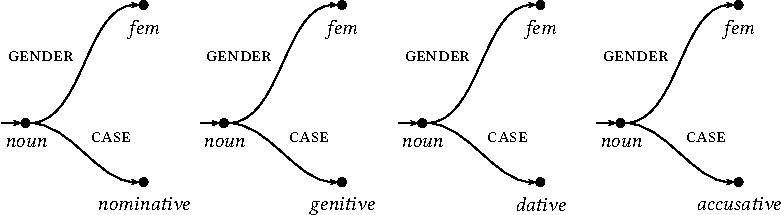
\includegraphics{Figures/frau-model-theoretic-cropped}
}
%%   \begin{pspicture}(-0.5,0.4)(2.8,4.1)
%% %\psgrid
%%      \psset{fillstyle=solid, fillcolor=black,radius=0.75mm}
%%      \pnode(-0.4,2){start1}
%%      \Cnode(0,2){noun1}
%%      \Cnode(2,4){fem1}
%%      \Cnode(2,1){nom1}
%% %
%%      \psset{fillstyle=none,nodesep=0pt,angleB=180,arrows=->} 
%% %
%%      \nccurve{start1}{noun1}
%%      \nccurve{noun1}{fem1}\naput{\textsc{gender}}
%%      \nccurve{noun1}{nom1}\naput{\textsc{case}}
%% %
%%      \nput{270}{noun1}{\type{noun}}
%%      \nput{270}{fem1}{\type{fem}}
%%      \nput{270}{nom1}{\type{nominative}}
%% \end{pspicture}
%% \begin{pspicture}(-0.5,0.4)(2.8,4.1)
%% %\psgrid
%% %
%%      \psset{fillstyle=solid, fillcolor=black,radius=0.75mm}
%%      \pnode(-0.4,2){start2}
%%      \Cnode(0,2){noun2}
%%      \Cnode(2,4){fem2}
%%      \Cnode(2,1){nom2}
%% %
%%      \psset{fillstyle=none,nodesep=0pt,angleB=180,arrows=->} 
%% %
%%      \nccurve{start2}{noun2}
%%      \nccurve{noun2}{fem2}\naput{\textsc{gender}}
%%      \nccurve{noun2}{nom2}\naput{~\textsc{case}}

%%      \nput{270}{noun2}{\type{noun}}
%%      \nput{270}{fem2}{\type{fem}}
%%      \nput{270}{nom2}{\type{genitive}}
%% \end{pspicture}
%% \begin{pspicture}(-0.5,0.4)(2.8,4.1)
%% %\psgrid
%%      \psset{fillstyle=solid, fillcolor=black,radius=0.75mm}
%%      \pnode(-0.4,2){start3}
%%      \Cnode(0,2){noun3}
%%      \Cnode(2,4){fem3}
%%      \Cnode(2,1){nom3}
%% %
%%      \psset{fillstyle=none,nodesep=0pt,angleB=180,arrows=->} 
%% %
%%      \nccurve{start3}{noun3}
%%      \nccurve{noun3}{fem3}\naput{\textsc{gender}}
%%      \nccurve{noun3}{nom3}\naput{\textsc{case}}
%% %
%%      \nput{270}{noun3}{\type{noun}}
%%      \nput{270}{fem3}{\type{fem}}
%%      \nput{270}{nom3}{\type{dative}}
%% \end{pspicture}
%% \begin{pspicture}(-0.5,0.4)(2.8,4.1)
%% %\psgrid
%%      \psset{fillstyle=solid, fillcolor=black,radius=0.75mm}
%%      \pnode(-0.4,2){start2}
%%      \Cnode(0,2){noun2}
%%      \Cnode(2,4){fem2}
%%      \Cnode(2,1){nom2}
%% %
%%      \psset{fillstyle=none,nodesep=0pt,angleB=180,arrows=->} 
%% %
%%      \nccurve{start2}{noun2}
%%      \nccurve{noun2}{fem2}\naput{\textsc{gender}}
%%      \nccurve{noun2}{nom2}\naput{\textsc{case}}
%% %
%%      \nput{270}{noun2}{\type{noun}}
%%      \nput{270}{fem2}{\type{fem}}
%%      \nput{270}{nom2}{\type{accusative}}
%% \end{pspicture}}
\caption{\label{abb-avm-frau}Feature structures for the description of \emph{Frau} `woman' in (\ref{avm-frau})}
\end{figure}%
%-----------------------------------------------------------------------------
\begin{figure}
%\oneline{%
\centerline{%
%% \begin{pspicture}(-0.5,0.4)(2.8,4.1)
%% %\psgrid
%% %
%% %
%%      \psset{fillstyle=solid, fillcolor=black,radius=0.75mm}
%%      \pnode(-0.4,2){start1}
%%      \Cnode(0,2){noun1}
%%      \Cnode(2,4){mas1}
%%      \Cnode(2,1){nom1}
%% %
%% %
%%      \psset{fillstyle=none,nodesep=0pt,angleB=180,arrows=->} 
%% %
%%      \nccurve{start1}{noun1}
%%      \nccurve{noun1}{mas1}\naput{\textsc{gender}}
%%      \nccurve{noun1}{nom1}\naput{\textsc{case}}
%% %
%%      \nput{270}{noun1}{\type{noun}}
%%      \nput{270}{mas1}{\type{mas}}
%%      \nput{270}{nom1}{\type{nominative}}
%% \end{pspicture}
%% \begin{pspicture}(-0.5,0.4)(2.8,4.1)
%% %\psgrid
%% %
%%      \psset{fillstyle=solid, fillcolor=black,radius=0.75mm}
%%      \pnode(-0.4,2){start2}
%%      \Cnode(0,2){noun2}
%%      \Cnode(2,4){mas2}
%%      \Cnode(2,1){nom2}
%% %
%% %
%%      \psset{fillstyle=none,nodesep=0pt,angleB=180,arrows=->} 
%% %
%%      \nccurve{start2}{noun2}
%%      \nccurve{noun2}{mas2}\naput{\textsc{gender}}
%%      \nccurve{noun2}{nom2}\naput{\textsc{case}}
%% %
%%      \nput{270}{noun2}{\type{noun}}
%%      \nput{270}{mas2}{\type{mas}}
%%      \nput{270}{nom2}{\type{dative}}
%% \end{pspicture}
%% \begin{pspicture}(-0.5,0.4)(2.8,4.1)
%% %\psgrid
%% %
%%      \psset{fillstyle=solid, fillcolor=black,radius=0.75mm}
%%      \pnode(-0.4,2){start2}
%%      \Cnode(0,2){noun2}
%%      \Cnode(2,4){mas2}
%%      \Cnode(2,1){nom2}
%% %
%% %
%%      \psset{fillstyle=none,nodesep=0pt,angleB=180,arrows=->} 
%% %
%%      \nccurve{start2}{noun2}
%%      \nccurve{noun2}{mas2}\naput{\textsc{gender}}
%%      \nccurve{noun2}{nom2}\naput{\textsc{case}}
%% %
%%      \nput{270}{noun2}{\type{noun}}
%%      \nput{270}{mas2}{\type{mas}}
%%      \nput{270}{nom2}{\type{accusative}}
%% \end{pspicture}
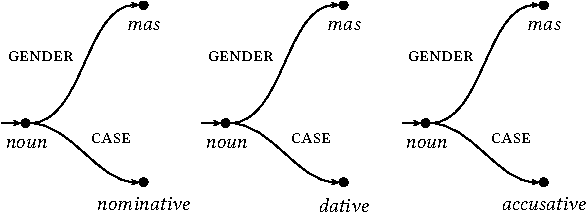
\includegraphics{Figures/mann-model-theoretic-crop}
}
\caption{\label{abb-avm-mann}Feature structures for the description of \emph{Mann} `man' in  (\ref{avm-mann})}
\end{figure}%
In these representations, each node has a certain type (\type{noun}, \type{fem}, \type{nominative},
\ldots) and the types in feature structures are always maximally specific, that is, they do not have
any further subtypes. There is always an entry node (\type{noun} in the example above) and the other
nodes are connected with arrows that are annotated with the feature labels (\textsc{gender}, \textsc{case}).

If we return to the example with people from the previous sections, we can capture the difference between a model and a description as follows:
if we have a model of people that includes first name, last name, date of birth, gender and hair color, then it follows that every object we model also has a birthday.
We can, however, decide to omit these details from our descriptions if they do not play a role for
stating constraints or formulating searches.

The connection between linguistic phenomena, the model and the formal theory is shown in Figure~\vref{abb-modell}.
\begin{figure}
\centerline{%
%{
%% \begin{pspicture}(0,0)(9.4,4.2)
%% %\psgrid
%% \rput[Bl](0,0){%
%% \begin{tabular}[b]{@{}ccc@{}}
%% phenomenon && model\\
%% \rnode{phen}{\fbox{\begin{tabular}{c}
%% linguistic\\
%% objects\\
%% \end{tabular}}}&&\rnode{modell}{\fbox{\begin{tabular}{c}
%% feature\\
%% structures\\
%% \end{tabular}}}\\[10ex]
%% &\rnode{theorie}{\fbox{\begin{tabular}{c}
%% feature\\
%% descriptions\\
%% \end{tabular}}}\\
%% &formal theory\\
%% \end{tabular}}
%% %\anodeconnect[l]{modell}[r]{phen}%
%% \ncline{->}{modell}{phen}\nbput{models}
%% %\ncdiag[angleA=180,angleB=45]{->}{modell}{theorie}
%% \psline{<-}(5.4,1.6)(6,2.4)
%% \rput[Bl](6,2){licensed by the theory} % früher Erfüllung, jetzt FR Änderung
%% \psline{->}(5,1.7)(5.6,2.4)
%% \rput[Bl](3.4,2.0){determines}
%% %\nccurve{<-}{modell}{theorie}\nbput{legt fest}
%% \ncline{->}{theorie}{phen}\naput{predicts}%
%% %\aanodeconnect[b]{modell}[tr]{theorie}%
%% %\anodeconnect[tl]{theorie}[b]{phen}%
%\end{pspicture}
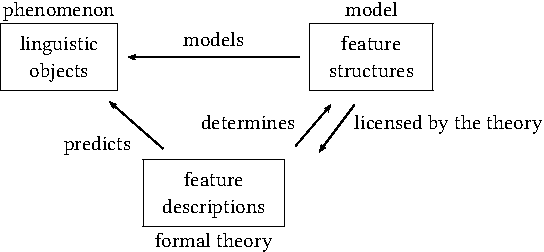
\includegraphics{Figures/model-theory-phenomenon-crop}
}
\caption{\label{abb-modell}Phenomenon, model and formal theory}
\end{figure}%
\nocite{Netter98a}%S. 26
%\NOTE{WS: zwischen Modell und Theorie sollten zwei Pfeile sein.}
% ###########
% zwei Pfeile: Beschreibung legt Modell fest , um Rekursion zu erfassen (beschreibt geht wohl auch, ist aber sloppy)
%
% Modell wird von der formalen Theorie lizenziert. 
%
% Phänomen + Modell -> PS: modelliert -> lassen wir so.
%
The model is designed to model linguistic phenomena. Furthermore, it must be licensed by our theory.
The theory determines the model and makes predictions with regard to possible phenomena.
\is{model|)}\is{theory|)}\is{Phenomenon|)}\is{feature description|)}\is{feature structure|)}

~\vspace{\baselineskip}
\questions{

\begin{enumerate}
\item What are the reasons for using types?
\item What is inheritance? What is special about multiple inheritance?
\item Are the following structures compatible, that is, can they be used to describe the same object? 
\ea
\onems{
firstname \type{max}\\
lastname \type{meier}\\
father    \ms[person]{
              firstname  & peter\\
              lastname & meier
             }
}\hspace{0.5cm}\onems{
firstname  \type{max}\\
lastname \type{meier}\\
father   \ms[person]{
              firstname  & peter\\
             lastname & müller
             }
}
\z
\ea
\onems{
firstname   \type{max}\\
lastname  \type{meier}\\
father     \ms[person]{
              firstname & peter\\
              lastname & meier
             }
}\hspace{0.5cm}\onems{
firstname   \type{max}\\
lastname  \type{meier}\\
mother      \ms[person]{
              firstname  & ursula\\
              lastname & müller
             }
}
\z

\end{enumerate}
}

\exercises{

\begin{enumerate}
\item Think about how one could describe musical instruments using feature descriptions.
\item Come up with a type hierarchy for the word classes (\type{det}, \type{comp}, \type{noun}, \type{verb},
      \type{adj}, \type{prep}). Think about the ways in which one can organize the type hierachy so that one
	  can express the generalizations that where captured by the binary features in Table~\ref{Tabelle-Merkmalszerlegung-Wortarten} on page~\pageref{Tabelle-Merkmalszerlegung-Wortarten}.
\item\label{ua-liste} In this chapter, we introduced lists. This may look like an extension of the formalism, but it is not as it is possible to
convert the list notation into a notation which only requires feature"=value pairs. Think about how one could do this.
\item (Additional exercise) The relation \emph{append}\is{relation!\emph{append}} will play a role in Chapter~\ref{Kapitel-HPSG}. This relation serves to
combine two lists to form a third.
Relational constraints such as \emph{append} do in fact constitute an expansion of the formalism. Using relational constraints, it is possible to relate any number
of feature values to other values, that is, one can write programs which compute a particular value depending on other values. 
This poses the question as to whether one needs such powerful descriptive tools in a linguistic theory and if we do allow them, what kind of complexity we afford them.
A theory which can do without relational constraints should be preferred over one that uses
relational constraints (see \citealp[Chapter~20]{MuellerLehrbuch1} for a comparison of theories).

For the concatenation of lists, there is a possible implementation in feature structures without
recourse to relational constraints. Find out how this can be done. Give your sources and document
how you went about finding the solution.

\end{enumerate}
}

\furtherreading{

This chapter was designed to give the reader an easy"=to"=follow introduction to typed feature structures. The mathematical properties of the structures, type hierarchies and the
combinatorial possibilities of such structures could not be discussed in detail here, but knowledge of
at least part of these properties is important for work in computational linguistics and in
developing one's own analyses. For more information, I refer the interested reader to the following publications: 
%
\citet{Shieber86a} is a short introduction to the theory of Unification Grammar. It offers a relatively general overview followed by the discussion of important grammar types
such as DCG\is{Definite Clause Grammar (DCG)}, \lfg, \gpsg,
HPSG, PATR-II\is{PATR-II}.
%
\citet{Johnson88} describes the formalism of untyped feature structures in a mathematically precise way.
%
\citet{Carpenter92a} goes into the detail about the mathematical aspects of typed feature structures. The formalism developed by \citet{King99a-u} for HPSG"=grammars forms the basis
for the formalism by \citet{Richter2004a-u}, which currently counts as the standard formalism for HPSG.
}

%      <!-- Local IspellDict: en_US-w_accents -->

%% -*- coding:utf-8 -*-

\chapter{Lexical Functional Grammar}
\label{Kapitel-LFG}


Lexical Functional Grammar (LFG) was developed in the 80s by Joan Bresnan and Ron Kaplan \citep{BK82a}. LFG forms part of
so"=called West-Coast linguistics: unlike MIT, where Chomsky works and teaches, the institutes of researchers such as Joan
Bresnan and Ron Kaplan are on the west coast of the USA (Joan Bresnan in Stanford and Ron Kaplan at Xerox in Palo Alto and now at the language technology firm
Nuance Communications in the Bay Area in California).


\citet{BK82a} view LFG explicitly as a psycholinguistically plausible alternative to transformation"=based approaches. For a discussion of
the requirements regarding the psycholinguistic plausibility of linguistics theories, see Chapter~\ref{Abschnitt-Diskussion-Performanz}. 

The more in"=depth works on German are \citew{Berman96a-u,Berman2003a} and \citew{Cook2001a}.

LFG has well-designed formal foundations \citep{KB82a-u,Kaplan95a}, and hence first implementations
were available rather quickly \citep*{FR83b,FR83a,Yasukawa1984a-u,BH86a-u,%
ED86a-u,% CHARON Parser
WA86a-u,%
Delmonte90a-u,% Italien
HHP91a-u,% Chinesisches kommerzielles System
Kohl92a-u,KGPRM92a-u,% ACORD project CHARON Generator
KM96a-u,%
Mayo97a-u,Mayo99a-u,%Konstanzer system
BS2005b-u,BS2005a-u,%SxLFG
Clement2009a-u,CK2001a-u% XLFG
}. 

The following is a list of languages with implemented LFG fragments, probably incomplete:
% Tracy 30.03.2010
%
% Hungarian is just starting in ParGram and so does not have any
% papers on the implementation.  Welsh does not have a good citation for
% the implemented grammar.  Spanish ParGram is only a toy grammar and
% has no publications.
%
% Lionel Clement (cc-ed here, hopefully with his correct address) has
% an LFG implementation which you might wish to include.  It has a web
% interface which makes it particularly nice for teaching.
%
% http://www.xlfg.org/
%
% Leonel de Alencar, 31.03.2010
% Es gibt tatsächlich viele ältere LFG-Systeme. Meines Wissens ist das in SWI-Prolog implementierte
% GFU-Lab das einzige, das noch funktioniert. Dieses System, das sich gut für den Unterricht eignet,
% ist aber kein orthodoxes LFG-System und z.B. mit LKB nicht vergleichbar.
%
% AdamP 25.05.2015 zu ParGram
%% . Hungarian
%% • Norwegien
%% • Urdu
%% • Wolof
%% • Turkish 
%% • Polish
%% • Georgian (toy grammar? – not sure)
%% • Slovenian (toy grammar? – not sure)
%% • Greek (rather preliminary work at the moment)
%% • German (not sure about current developments)
%% • English (not developed for some time)
%% • French (not developed for a long time)



\begin{itemize}
\item Arabic\il{Arabic} \citep{Attia2008a-u},
\item Arrernte\il{Arrernte} \citep*{Dras2012a-u},
\item Bengali\il{Bengali} \citep{SC97a-u},
%\item Chinese\il{Mandarin Chinese}
\item Danish\il{Danish} \citep{Oersnes2002b-u,OW2003a-u,OW2004a-u},
\item English\il{English} \citep*{HHP91a-u,BDFK99a-u,RKKCMJ2002a-u,KM2007a-u},
\item French\il{French} \citep*{Zweigenbaum91a-u,Frank96b-u,FZ2002a-u,BDFK99a-u,CK2001a-u,BSL2005a-u,SdA2016a-u,Alencar2017a-u},
% Knueppel2001a-u
%
%
\item Georgian\il{Georgian} \citep{Meurer2009a-u},
\item German \citep{Rohrer96a,Berman96a-u,KR97a-u,BDFK99a-u,Dipper2003a-u,RF2006a,Forst2006a-u,Frank2006a-u,FR2009a-u},
%\item Griechisch\il{Griechisch},
\item Hungarian\il{Hungarian} \citep{LRT2010a-u},
\item Indonesian\il{Indonesian} \citep*{AADMS2009a-u},
\item Italian\il{Italian} \citep*{Delmonte90a-u,Mayo99a-u,Quaglia2012a-u},
\item Irish\il{Irish} \citep{Sulger2009a-u,Sulger2010a-u},
\item Japanese\il{Japanese} \citep*{HHP91a-u,MO2003a-u,Umemoto2006a-u},
\item Korean\il{Korean} \citep*{HHP91a-u},
\item Malagasy\il{Malagasy} \citep*{Randriamasimanana2006a-u,DLM2006a-u},
\item Mandarin Chinese\il{Mandarin Chinese} \citep*{HHP91a-u,FK2007a-u},
\item Murrinh-Patha\il{Murrinh-Patha} \citep{SN2012a-u},
\item Norwegian\il{Norwegian} \citep*{DMR2005a},
\item Polish\il{Polish} \citep*{PP2012a-u},
\item Portuguese\il{Portuguese} \citep{Alencar2004a-u,Alencar2013a-u,Alencar2015a-u},

% Tracy: Toy
% Forst:
% Apart from that, I have a little Spanish grammar, but it's very phenomenon-driven, not broad-coverage by any means and not documented anywhere, let alone in publications. 
\item Spanish\il{Spanish} \citep{Mayo99a-u},
%
% klein?
%\item Thai
\item Tigrinya\il{Tigrinya} \citep{Kifle2012a-u},
\item Turkish\il{Turkish} \citep{CO2006a-u},
\item Hungarian\il{Hungarian} \citep*{LRT2010a-u,RLC2011a-u},
% Journal-Artikel, aber unklar ob implementiert
\item Urdu/Hindi\il{Urdu}\il{Hindi} \citep*{BHKR2007a-u,BBS2008a-u},

% Forst: nichts mehr gehört
%\item Vietnamesisch\il{Vietnamesisch}
\item Welsh\il{Welsh} \citep{MS2005a-u}
and
\item Wolof\il{Wolof} \citep{Dione2012b-u,Dione2013a-u}.
\end{itemize}
Many of theses grammars were developed in the ParGram consortium\footnote{%
  \url{http://pargram.b.uib.no/research-groups/}. 2018-02-20.
} \citep*{BKNS99a-ed,BDKMR02a-u}. Apart from these grammars there is a small fragment of Northern
Sotho\il{Northern Sotho}, which is currently being expanded \citep{Faasz2010a-u}. 

%Im ParGram"=Projekt wird angestrebt, alle Sprachen mit den gleichen funktionalen Strukturen zu
%analysieren. Die Konstituentenstruktur wird als einzelsprachlich  angesehen

Many of the LFG systems combine linguistically motivated grammars with a statistical
component.\is{statistics} Such a component can help to find preferred readings of a sentence first,
it can increase the efficiency of processing and make the complete processing robust (for instance
\citealp{KRKMVC2004a-u,RKKCMJ2002a-u}). Josef van Genabith's group in Dublin is working on the induction of
LFG grammars from corpora (\eg \citealp{JGCCR99a-u,DBCGW2005a-u,CBFDRCW2005a-u,CG2006a-u,GWG2007a-u,CBDRGW2008a-u,SG2009a-u}). 

\pagebreak
Some of the systems can be tested online:
\begin{itemize}
\item \url{http://iness.uib.no/xle-web/xle-web}

% Statistik Dublin
%\item \url{http://lfg-demo.computing.dcu.ie/lfgparser.html}
\item \url{http://www.xlfg.org/}
\end{itemize}




\section{General remarks on the representational format}
\label{Abschnitt-Format-LFG}

LFG assumes multiple levels of representation.\footnote{%
	The English examples and their analyses discussed in this section are taken from
        \citet{Dalrymple2001a-u} and \citet{Dalrymple2006a}.
} The most important are c"=structure\is{c"=structure} and f"=structure\is{f"=structure}. c"=structure is the constituent
structure and it is licensed by a phrase structure grammar. This phrase structure grammar uses
\xbar~structures for languages for which this is appropriate. f"=structure stands for functional structure. Functional structure contains information about the predicates involved
and about the grammatical functions (subject, object, \ldots) which occur in a constituent. Mappings
mediate between these representational levels.


\subsection{Functional structure}

In LFG, grammatical functions such as subject and object play a very important role. Unlike in most other theories discussed in this book, they are primitives
of the theory. A sentence such as (\mex{1}a) will be assigned a functional structure as in (\mex{1}b):


\eal
\ex David devoured a sandwich.
\ex \lfgms{ pred & `DEVOUR\sliste{\lfgsubj, \lfgobj}'\\
         subj & \lfgms{ pred &  `DAVID' \\
                   }\\
         obj  & \lfgms{ spec & A\\
                     pred & `SANDWICH'\\
                   }\\
       }
\zl

\noindent
All lexical items that have a meaning (\eg nouns, verbs, adjectives) contribute a \textsc{pred}\isfeat{pred} feature with a corresponding value.
The grammatical functions governed by a head (government = subcategorization)
are determined in the specification of \textsc{pred}.\footnote{%
In the structure in (\mex{0}b), the \lfgsubj{} and \lfgobj{} in the list following \emph{devour} are identical to the values of \lfgsubj{} and \lfgobj{} in the structure. For reasons of presentation, this will not be explicitly indicated in this structure and following structures.
}
Corresponding functions are called \emph{governable grammatical functions}\is{grammatical function!governable}. Examples of this are shown in Table~\vref{Tabelle-GOV} \citep{Dalrymple2006a}.
\begin{table}
\centering
\begin{tabular}[t]{@{}lp{26em}@{}} 
\lsptoprule
\textsc{subj}\isfeat{subj}: & subject \\ 
%
\textsc{obj}\isfeat{obj}: & object\\ 
%
\textsc{comp}\isfeat{comp}: & sentential complement or closed (non-predicative) infinitival complement\\
\textsc{xcomp}\isfeat{xcomp}: & open (predicative) complement, often infinitival, the \textsc{subj} function
is externally controlled\is{control}\\
\objtheta: & secondary \textsc{obj} functions that are related to a special, language \\
           & specific set of grammatical roles; English has \objtheme only.\\
%
\obltheta: & a\isfeat{obl} group of thematically restricted oblique functions, as for instance
         {\obl\downlett{GOAL}} or {\obl\downlett{AGENT}}. These often correspond to adpositional
         phrases in c-structure.\\
\lspbottomrule
\end{tabular}
\caption{\label{Tabelle-GOV}Governable grammatical functions}
\end{table}\todostefan{\objtheta im Deutschen?}%
The \pred specification corresponds to the theta grid\is{theta-grid@$\theta$-grid} in \gbt. The valence\is{valence} of a head is specified by
the \predv.

The non"=governable grammatical functions are given in Table~\vref{Tabelle-NGOV}.
\begin{table}
\centering
\begin{tabular}[t]{@{}lp{26em}@{}} 
\lsptoprule
\textsc{adj}\isfeat{adj}: & adjuncts \\ 
%
\textsc{topic}\isfeat{topic}: & the topic of an utterance\\ 
%
\textsc{focus}\isfeat{focus}: & the focus of an utterance\\
\lspbottomrule
\end{tabular}
\caption{\label{Tabelle-NGOV}Non-governable grammatical functions}
\end{table}%
Topic\is{topic|(} and focus\is{focus|(} are information"=structural\is{information structure} terms. There are a number of works on their exact definition, which differ to
varying degrees \citep[\page 253--254]{KruijffSteedman2003}, but broadly speaking, one can say that the focus of an utterance constitutes new information and that
the topic is old or given information. \citet[\page 97]{Bresnan2001a} uses the following question tests in order to determine topic and focus:

\ea
\label{bsp-fronted-focus}
Q: What did you name your cat?\\
A: Rosie I named her. (\emph{Rosie} = \textsc{focus})
\z
\ea
\label{bsp-fronted-topic}
Q: What did you name your pets?\\
A: My dog, I named Harold. My cat, I named Rosie. (\emph{my dog}, \emph{my cat} = \textsc{topic})
\z
\is{topic|)}\is{focus|)}

\noindent
f"=structures are characterized using functional descriptions, for example, one can refer to a value of the feature \textsc{tense} in the functional structure $f$
using the following expression:

\ea
($f$ \lfgtense)
\z

\noindent
It is possible to say something about the value which this feature should have in the feature description. The following descriptions express the fact that in the structure $f$,
the feature \lfgtense{} must have the value \lfgpast.

\ea
($f$ \lfgtense) = \lfgpast
\z

\noindent
The value of a feature may also be a specific f"=structure. The expression in (\mex{1})
ensures that the \subjf in $f$ is the f"=structure $g$:

\ea
\label{ex-LFG-constraint}
($f$ \lfgsubj) = $g$
\z

\noindent
For the analysis of (\mex{1}a), we get the constraints in (\mex{1}b):
\eal
\ex David sneezed.
\ex
\begin{tabular}[t]{l}
($f$ \pred) = {\small `SNEEZE\arglist{\lfgsubj}'}\\
($f$ \lfgtense) = \lfgpast\\
($f$ \lfgsubj) = $g$\\
($g$ \pred) = {\small `DAVID'}
\end{tabular}
\zl

\noindent
The description in (\mex{0}b) describes the following structure:
\ea
$f$: \lfgms{ pred  & {\small `SNEEZE\arglist{\lfgsubj}'}\\
             tense & \lfgpast\\
             subj  & $g$: \onems{ pred {\small `DAVID'} }\\
        }
\z

\noindent
But (\mex{-1}b) also describes many other structures which contain further features. We are only
interested in minimal structures that contain the information provided in the description.

(\mex{1}) shows how a node in the c"=structure can be connected to the f"=structure for the entire sentence:

\ea
%\ex David sneezed.
%\ex 
%% \begin{tabular}[t]{@{}ll@{}}
%% \begin{tabular}[t]{@{}cc@{}}
%% \multicolumn{2}{c}{\rnode{ip}{IP}}\\[2ex]
%% \rnode{b}{\rnode{np}{NP}}       & \rnode{i1}{I$'$}\\[2ex]
%% \rnode{n1}{N$'$}     & \rnode{vp}{VP}\\[2ex]     
%% \rnode{n}{N}         & \rnode{v1}{V$'$}\\[2ex]   
%% \rnode{David}{David} & \rnode{v}{V}\\[2ex]       
%%                     & \rnode{sneezed}{sneezed}\\
%% \end{tabular}
%% &
%% \lfgms{
%% pred & `SNEEZE\arglist{\lfgsubj}'\\
%% tense & PAST\\
%% subj  & \rnode{i}{\lfgms{ pred & `DAVID' \\
%%                       }}\\
%% }\\
%% \ltor[-15]{b}[175]{i}
%% \Aput*{$\phi$}
%% \end{tabular}
\tree{IP}{%
  \tree[b]{NP}{\tree{N$'$}{\tree{N}{\le{David}}}}
  \tree{I$'$}{\tree{VP}{\tree{V$'$}{\tree{V}{\le{sneezed}}}}}}%
\hspace*{4em}%
\raisebox{-2em}{\lfgms{
pred & {\small `SNEEZE\arglist{\lfgsubj}}'\\
tense & \lfgpast\\
subj  & \rnode{i}{\lfgms{ pred & {\small `DAVID'} \\
                      }}\\
}}\\
\ltor[-15]{b}[175]{i}
\Aput*{$\phi$}
\z
The function $\phi$ from the NP"=node to the f"=structure corresponding to the NP is depicted with an arrow marked $\phi$.

A phrase and its head always correspond to the same f"=structure:

\ea
\begin{tabular}[t]{@{}c@{}}
\rnode{a}{\rnode{v1}{V$'$}}\\[2ex]
\rnode{b}{\rnode{v}{V}}\\[2ex]
\rnode{sneezed}{sneezed}\\
\end{tabular}
\hspace*{4em}
\rnode{d}{\raisebox{-2em}{\lfgms{ pred & {\small `SNEEZE\arglist{\lfgsubj}'}\\
                                  tense & \lfgpast}}}
\ncline{v1}{v}\ncline{v}{sneezed}%
\ltor{a}{d}
\Aput*{$\phi$}
\ltor{b}{d}
\z

\noindent
In LFG grammars of English, the CP/IP system is assumed as in \gbt (see Section~\ref{Abschnitt-GB-CP-IP-System-Englisch}). IP, I$'$ and I
(and also VP) are mapped onto the same f"=structure.

\eal
\ex David is yawning.

\ex {\tree[a]{IP}{%
  \tree{NP}{\tree{N$'$}{%
    \tree{N}{\le{David}}}}
  \tree[b]{I$'$}{%
    \tree[c]{I}{\le{is}}
    \tree[d]{VP}{\tree[e]{V$'$}{\tree[f]{V}{\le{yawning}}}}}}}%
\hspace*{4em}%
{\rnode{o}{\raisebox{-2em}{\lfgms{ pred & {\small `YAWN\arglist{\lfgsubj}'}\\
                                   tense & \lfgpres\\
                                   subj  & \lfgms{ pred & {\small `DAVID'}}}}}}
\ltor{a}{o}
\ltor{b}{o}
\ltor[10]{c}{o}
\ltor{d}{o}
\ltor{e}{o}
\ltor{f}{o}
\zl



%% \subsubsection{Funktionale Eindeutigkeit ({\em Functional Uniqueness})}

%% {
%% {Funktionale Eindeutigkeit ({\em Functional Uniqueness})}

%% }

\noindent
f"=structures have to fulfill two well"=formedness conditions: they have to be both \emph{complete} and \emph{coherent}. Both these conditions will be
discussed in the following sections.

\subsection{Completeness}

Every head adds a constraint of the \textsc{pred} value of the corresponding f"=structure. In determining completeness, one has to check that the elements required
in the \textsc{pred} value are actually realized. In (\mex{1}b), \textsc{obj} is missing a value, which is
why (\mex{1}a) is ruled out by the theory.

\eal
\ex[*]{David devoured.
}
\ex[]{
\lfgms{ pred & {\small `DEVOUR\sliste{\lfgsubj,\lfgobj}'}\\
         subj & \lfgms{ pred & {\small `DAVID'} \\
                   }\\
       }
}
\zl

\subsection{Coherence}

\addlines
The Coherence Condition requires that all argument functions in a given f"=structure have to be selected in the value of the local 
 \textsc{pred} attribute. (\mex{1}a) is ruled out because \textsc{comp} does not appear under the arguments of \emph{devour}.

\eal
\ex[*]{
David devoured a sandwich that Peter sleeps.%\\
%`David verschlang ein Sandwich, daß Peter schläft.'
}
\ex[]{
\lfgms{ pred & {\small `DEVOUR\sliste{\lfgsubj,\lfgobj}'}\\
         subj & [ \textsc{pred} {\small `DAVID'} ] \\
         obj  & \lfgms{ spec &  A\\
                     pred & {\small `SANDWICH'}\\
                   }\\
         comp & \lfgms{ pred & {\small `SLEEP\sliste{\lfgsubj}'}\\
                        subj & \lfgms{ pred & {\small `PETER'}\\
                                     }\\
                   } 
       }
}
\zl

\noindent
The constraints on completeness and coherence together ensure that all and only those arguments required in
the \pred specification are actually realized.
Both of those constraints taken together correspond to the Theta"=Criterion\is{theta-criterion@Theta"=Criterion} in \gbt (see
page~\pageref{theta-Kriterium}).\footnote{%
For the differences between predicate"=argument structures in LFG and the Deep Structure oriented Theta Criterion, see \citew[\page xxvi--xxviii]{BK82a}.} 

\subsection{Restrictions on the c-structure/f-structure relation}

\largerpage
Symbols in c"=structures\is{c"=structure|(} are assigned restrictions for f"=structures. The following symbols are used: `\up'\is{$\uparrow$} refers to the f"=structure of the
immediately dominating node and `$\downarrow$'\is{$\downarrow$} refers to the f"=structure of the c"=structure node bearing the annotation. A common annotation is
`\up~=~\down'. This constraint states that the f"=structure of the mother node is identical to that of the annotated category:

\ea
V$'$ $\to$ \begin{tabular}[t]{@{}r@{~=~}l@{}}
           \multicolumn{2}{@{}l@{}}{\hspaceThis{f-structure of the mother~}V}\\
           $\uparrow$ &  $\downarrow$\\ 
           f-structure of the mother & own f-structure\\
           \end{tabular}
\z
The annotation `\up~=~\down' is below the head\is{head} of a structure.

Phrases which are licensed by the annotated c"=structure in (\mex{0}) can be visualized as follows:
\ea
\talltree[a]{V$'$}{\le[b]{V}}%
\hspace*{3em}%
\rnode{d}{[\ ]}
\ltor{a}{d}
\ltor{b}{d}
\z

\noindent
(\mex{1}) shows a V$'$~rule with an object:
\ea
\phraserule{V$'$}{
\rulenode{V\\* \up~=~\down}
\rulenode{NP\\*(\up\ \lfgobj) = \down}}
\z
%
The annotation on the NP signals that the \textsc{obj} value in the f"=structure of the mother
\mbox{(\up\ \lfgobj)} is identical to the f"=structure of the NP node, that is, to everything that is
contributed from the material below the NP node (\down). 
This is shown in the figure in (\mex{1}):
\ea
\talltree[a]{V$'$}{\le[b]{V} \le[c]{NP}}%
\hspace*{3em}%
\rnode{d}{\fd{\fdand{\feat{\lfgobj}{\rnode{e}{[\ ]}}}}}
\ltor{a}{d}
\ltor[20]{b}{d}
\ltor{c}[190]{e}
\z
In the equation (\up\ \lfgobj) = \down{},  the arrows `\up' and `\down' correspond to feature structures. `\up' and
`\down' stand for the $f$ and $g$ in equations such as (\ref{ex-LFG-constraint}).

(\mex{1}) is an example with an intransitive verb and (\mex{2}) is the corresponding visualization:

\ea
\catlexentry{sneezed}{V}{(\up\ \pred) = {\small `SNEEZE\arglist{\lfgsubj}'}\\*
                     (\up\ \lfgtense) = \lfgpast}
\z

\ea
\tree{V}{\le{sneezed}}
\hspace*{4em}
\rnode{d}{\mbox{\lfgms{ pred & {\small `SNEEZE\arglist{\lfgsubj}'}\\
                        tense & \lfgpast}}}
\ltor{top}{d}
\z
\is{f"=structure|)}\is{c"=structure|)}\il{English|)}

\subsection{Semantics}
\label{lfg-semantics}
\label{glue-semantics}

Following \citet[\page 90--92]{Dalrymple2006a}, \emph{glue semantics}\is{glue semantics|(} is the dominant approach to semantic interpretation in LFG
(\citealp*{DLS93a-u}; \citealp[Chapter~8]{Dalrymple2001a-u}). There are, however, other variants
where Kamp's discourse representation structures \citep{KR93a} are used \citep{FR83b,FR83a}.

In the following, glue semantics will be presented in more detail.\footnote{%
%The following section is a translation of the corresponding section in  \citew{Dalrymple2006a}.
The following discussion heavily draws from the corresponding section of \citew{Dalrymple2006a}. (It
is a translation of my translation of the original material into German.)
}
Under a glue"=based approach, it is assumed that f"=structure is the level of syntactic representation which is crucial for the semantic interpretation of
a phrase, that is, unlike \gbt, it is not the position of arguments in the tree which play a role in the composition of meaning, but rather functional relations such as 
\lfgsubj and \lfgobj. Glue semantics assumes that each substructure of the f"=structure corresponds to a semantic resource connected to a meaning and furthermore, that the meaning
of a given f"=structure comes from the sum of these parts. The way the meaning is assembled is
regulated by certain instructions for the combination of semantic resources. These instructions are given
as a set of logic premises written in linear logic\is{linear logic} as \emph{glue language}\is{glue language}. The computation of the meaning of an utterance corresponds to a logical conclusion.

%\addlines[2]
This conclusion is reached on the basis of logical premises contributed by the words in an
expression or possibly even by a syntactic construction itself. The requirements on how the meaning
of the parts can be combined to yield the full meaning are expressed in linear logic, a
resource"=based logic. Linear logic is different from classic logic in that it does not allow that
premises of conclusions are not used at all or more than once in a derivation. Hence, in linear logic, premises
are resources which have to be used. This corresponds directly to the use of words in an expression:
words contribute to the entire meaning exactly once. It is not possible to ignore them or to use
their meaning more than once. A sentence such as \emph{Peter knocked twice.} does not mean the same as \emph{Peter knocked}. The meaning of
\emph{twice} must be included in the full meaning of the sentences. Similarly, the sentence cannot
mean the same as \emph{Peter knocked twice twice.}, since the semantic contribution of a given word cannot be used twice.

The syntactic structure for the sentence in (\mex{1}a) together with its semantic representation is
given in (\mex{1}b):
%Figure~\vref{c-f-sem-david-yawned}:
\eal
\ex David yawned.
\ex ~\\[-\baselineskip]
\hspace*{-2em}
{\ctree[ip]{IP}{%
  \tree[b]{NP}{\tree[n]{N}{\le{\em David}}}
  \tree[ii]{I$'$}{\tree[vp]{VP}{\tree[v]{V}{\le{\em yawned}}}}}}%
\hspace*{3em}%
{\fd{\rnode{s}{\fdand{\feat{\pred}{\small `YAWN\arglist{\subj}'}
           \feat{\subj}{\rnode{i}{\fdand{\feat{\pred}{\small `DAVID'}}}}}}}}%
\hspace*{2em}%
\mt{\relation{yawn}(\relation{david})}{\rnode{x}{~[\ ]}}
\ltor{ip}{s}
\Aput*{$\phi$}
\ltord[-10]{s}[220]{x}
\Bput*{$\sigma$}
\zl
%% \begin{figure}
%% \centerline{%
%% {\ctree[ip]{IP}{%
%%   \tree[b]{NP}{\tree[n]{N}{\le{David}}}
%%   \tree[ii]{I$'$}{\tree[vp]{VP}{\tree[v]{V}{\le{yawned}}}}}}%
%% \hspace*{3em}%
%% {\rnode{s}{\lfgms{ pred & {\small `YAWN\arglist{\lfgsubj}'}\\
%%                    subj & \rnode{i}{[ \textsc{pred} {\small `DAVID'} ]}}}}%
%% \hspace*{2em}%
%% \mt{\relation{yawn}(\relation{david})}{\rnode{x}{\;[\ ]}}
%% \ltor{ip}{s}
%% \Aput*{$\phi$}
%% \ltord[-10]{s}[220]{x}
%% \Bput*{$\sigma$}
%% }
%% \caption{c-structure, f-structure and semantics of \emph{David yawned.}}\label{c-f-sem-david-yawned}
%% \end{figure}%
% 
The semantic structure of this sentence is connected to the f"=structure via the correspondence function $\sigma$ (depicted here as a dashed line). The semantic representation is
derived from the lexical information for the verb \emph{yawned}, which is given in (\mex{1}).

\ea
\mt{\lambda x. \relation{yawn}(x)}{(\up\ \lfgsubj)_\sigma\ \linimp\ \ups}
\z

\noindent 
This formula is referred to as the \emph{meaning constructor}\is{meaning constructor}. Its job is to combine the meaning of \emph{yawned} -- a one place predicate
$\lambda x. \relation{yawn}(x)$ -- with the formula\is{\linimp}
\mbox{$(\up\ \lfgsubj)_\sigma\ \linimp\ \ups$} in linear logic. Here, the connective \linimp\ is the
\emph{linear implication} symbol of linear logic. The symbol contains the meaning that \emph{if} a
semantic resource $(\up\;\lfgsubj)_\sigma$ for the meaning of the subject is available,
\emph{then} a semantic resource for $\up_\sigma$ must be created which will stand for the entire meaning of the sentence.
Unlike the implication operator of classic logic, the linear implication must consume and produce
semantic resources: the formula \mbox{$(\up\ \lfgsubj)_\sigma\ \linimp\ \ups$} states that if a
semantic resource \mbox{$(\up\  \lfgsubj)_\sigma$} is found, it is consumed and the semantic resource
\ups is produced.

Furthermore, it is assumed that a proper name such as \emph{David} contributes its own semantic structure as a semantic resource. In an utterance such as \emph{David yawned},
this resource is consumed by the verb \emph{yawned}, which requires a resource for its \lfgsubj in order to produce the resource for the entire sentence. This corresponds to the intuition
that a verb in any given sentence requires the meaning of its arguments in order for the entire sentence to be understood.
  
The f"=structure of \emph{David yawned} with the instantiated meaning construction contributed by \emph{David} and \emph{yawned} is given in (\mex{1}):

\eanoraggedright
 ~\\[-\baselineskip]
\fd{$y:$\rnode{s}{\fdand{\feat{\textsc{pred}}{\small `YAWN\arglist{\lfgsubj}'}
           \feat{\textsc{subj}}{$d:$\fdand{\feat{\textsc{pred}}{\small `DAVID'}}}}}}~\\[1em]
{$\begin{array}[t]{lr@{\;:\;}l}
\BF{David}&{\relation{david}}&{d_\sigma}\\*[1ex]
\BF{yawn}&{\lambda x. \relation{yawn}(x)}&{d_\sigma \linimp\ y_\sigma}
\end{array}$}
\z

\noindent 
The left side of the meaning constructor marked by \BF{David} is the meaning of the proper name \emph{David}, \relation{david} to be precise. The left"=hand side of the
meaning constructor \BF{yawn} is the meaning of the intransitive verb -- a one"=place predicate $\lambda x. \relation{yawn}(x)$.

Furthermore, one must still postulate further rules to determine the exact relation between the right"=hand side (the glue) of the meaning constructors in (\mex{0}) and the
left"=hand side (the meaning). For simple, non"=implicational meaning constructors such as
\BF{David} in (\mex{0}), the meaning on the left is the same as the meaning of the semantic structure on the right.
Meaning constructors such as \BF{yawn} have a $\lambda$"=expression on the left, which has to be combined with another expression via functional application (see
Section~\ref{sec-PSG-Semantik}). The linear implication on the right"=hand side must be applied in parallel. This combined process is shown in (\mex{1}).

\ea
\label{ex:curryhoward}
$\begin{array}[t]{r@{\;:\;}l}
{x} & {f_\sigma}  \\
{P} & {f_\sigma\ \linimp\ g_\sigma} \\
\hline
{P(x)} & {g_\sigma}
\end{array}$
\z
The right"=hand side of the rule corresponds to a logical conclusion following the \emph{modus ponens}\is{modus ponens} rule.
With these correspondences between expressions in linear logic and the meanings themselves, we can
proceed as shown in (\mex{1}), which is based on \citew[\page 92]{Dalrymple2006a}.
\begin{figure}[htb]
\ea
\label{ex:davidyawneddeduction}
\begin{tabular}[t]{r@{~:~}lp{18em}}
{\relation{david}} & $d_\sigma$ & The meaning \relation{david} is associated with the semantic structure of \lfgsubj\ 
$d_\sigma$.\\[1em] $\lambda
x. \relation{yawn}(x)$ & $d_\sigma \linimp\ y_\sigma$ & If we find the semantic resource for the \lfgsubj\ $d_\sigma$ on the glue side, 
this resource is consumed and the semantic resource for the entire sentence $y_\sigma$ is produced. On the meaning side,
we apply the function $\lambda x. \relation{yawn}(x)$ to the meaning associated with $d_\sigma$.\\[1em]
\hline\multicolumn{3}{c}{}\\
$\relation{yawn}(\relation{david})$ & $y_\sigma$ &
We have created the semantic structure $y_\sigma$ for the entire sentence, associated with the meaning of 
\relation{yawn}(\relation{david}).
\end{tabular}
\z
\vspace{-\baselineskip}
\end{figure}%
%
%\noindent 
After combining the respective meanings of \emph{yawned} and \emph{David} and then carrying out $\beta$"=reduction, we arrive at the desired result of
 $\relation{yawn}(\relation{david})$ as the
meaning of \emph{David yawned}.

Glue analyses of quantification\is{quantification}, modification and other phenomena have been investigated in a volume on glue semantics \citep{Dalrymple99a-ed}. Particularly
problematic for these approaches are cases where there appear to be too many or too few resources for the production of utterances. These kinds of cases have been discussed
by \citet{Asudeh04a-u}\is{glue semantics|)}.

\subsection{Adjuncts}
\label{Abschnitt-LFG-Adjunkte}

Adjuncts\is{adjuncts|(} are not selected by their head. The grammatical function \textsc{adj}\isfeat{adj} is a non"=governable grammatical function. Unlike arguments, where every grammatical
function can only be realized once, a sentence can contain multiple adjuncts. The value of \textsc{adj} in the f"=structure is therefore not a simple structure as with the other
grammatical functions, but rather a set. For example, the f structure for the sentence in (\mex{1}a)
contains an \textsc{adj} set with two elements: one for \emph{yesterday} and one for \emph{at noon}.
\eal
\ex\label{ex-david-devoured-a-sandwich-at-noon-yesterday} David devoured a sandwich at noon yesterday.
\ex\label{fstruc-david-devoured-a-sandwich-at-noon-yesterday} 
\lfgms{ pred & `DEVOUR\sliste{\lfgsubj,\lfgobj}'\\
         subj & \lfgms{ pred &  `DAVID' \\
                      }\\
         obj  & \lfgms{ spec & A\\
                        pred & `SANDWICH'\\
                      }\\
         adj & \menge{ \lfgms{ pred & `YESTERDAY' },
                        \lfgms{ \pred & `AT\arglist{\lfgobj}'\\
                                obj   & \lfgms{ pred & `NOON' }\\
                              } }\\
}
\zl
%
The annotation on the c"=structure rule for adjuncts requires that the f"=structure of the adjuncts
be part of the \textsc{adj} set of the mother's f"=structure:
\ea
\phraserule{V$'$}{
\rulenode{V$'$\\* \up~=~\down}
\rulenode{PP\\*\hbox {$\downarrow$\kern .2em} $\in$ (\up\ \adj)}}
\z
The representation of adjuncts in a set is not sufficient to characterize the meaning of an
utterance containing scope"=bearing\is{scope} adjuncts (as for instance the negation in sentences like (\ref{bsp-absichtlich-nicht-anal})
on page~\pageref{bsp-absichtlich-nicht-anal}). In order to determine scopal relations, one has to
refer to the linear order of the adjuncts, that is, the c"=structure. For linearization
restrictions\is{linearization rule} in LFG, see \citew{ZK95b}.\is{adjunct|)} 

\section{Passive}
\label{Abschnitt-LFG-Passiv}

%Banksy: "If you don't own a train company then you go and paint on one instead."
% Bindung in ein Kompositum hinein, aber sehr merkwürdig.
% en.wikipedia.org/wiki/Banksy 20.01.2013

\mbox{}\citet{BM95a} argue\is{passive|(}\is{morphology|(} that one should view words as ``atoms'' of
which syntactic structure is comprised (\emph{lexical integrity}\is{lexical integrity}\footnote{%
 See \citew[\page 84]{Anderson92a-u} for more on lexical integrity.%
}).

Syntactic rules cannot create new words or make reference to the internal structure of words. Every terminal node (each ``leaf'' of the tree) is a word. It follows from this that
analyses such as the GB analysis of \citet{Pollock89a-u} in Figure~\vref{abb-Pollock} for the French example in (\mex{1})  are ruled out (the figure is taken from
\citealp[\page 617]{Kuhn2007a}): 

% Felix sagt: So ist es richtig. Weicht von Jonas ab.
\ea
\gll Marie ne parlerait pas \\
     Marie \textsc{neg} speak.\textsc{cond.3sg} \textsc{neg}\\
\glt `Marie would not speak.'
\z
%
In Pollock's analysis, the various morphemes are in specific positions in the tree and are combined only after certain movements have been carried out.

\begin{figure}
\centerline{%
\begin{forest}
for tree={parent anchor=south, child anchor=north,align=center,base=bottom}
[AgrP
	[Spec-AgrP,name=specagr]
	[Agr$'$
		[Agr
			[\textit{-ait},name=ait]]
		[NegP
			[Spec-NegP
				[\textit{pas},name=pas]]
			[Neg$'$
				[Neg
					[\textit{ne},name=ne]]
				[TP
					[Spec-TP]
					[T$'$
						[T
							[\textit{-er-},name=er]]
						[VP
							[Spec-VP
								[\textit{Marie},name=marie]]
							[V$'$
								[V
									[\textit{parl-},name=parl]]]]]]]]]]
\begin{pgfinterruptboundingbox}% otherwise the picture gets larger due to the control points
\draw[->,dotted] (parl.south west) .. controls +(225:1cm) and +(south:0.4cm) .. (er.south);
\draw[->,dotted] (er.south west) .. controls +(left:1cm) and +(south:0.4cm) .. (ne.south);
\draw[->,dotted] (ne.south west) .. controls +(left:1cm) and +(south:0.4cm) .. (ait.south);
\draw[->,dotted] (marie.-90) .. controls +(225:6cm) and +(250:3cm) .. (specagr.-90);
\end{pgfinterruptboundingbox}
\end{forest}
}\is{category!functional!Neg}\is{category!functional!T}\is{category!functional!Agr}
\caption{\label{abb-Pollock} Pollock's analysis of \emph{Marie ne parlerait pas} `Marie would not
  speak.' according to \citet[\page 617]{Kuhn2007a}}
\end{figure}%
The assumption of lexical integrity is made by all theories discussed in this book with the
exception of GB and Minimalism. However, formally, this is not a must as it is also possible to
connect morphemes to complex syntactic structures in theories such as Categorial Grammar, GPSG,
HPSG, CxG, DG and TAG \citep[Section~4]{MuellerLexicalism}. As far as I know, this kind of analysis has never been proposed. 

%\subsection{Passiv als lexikalischer Prozeß}

Bresnan noticed that, as well as passivized verbs, there are passivized adjectives which show the same morphological idiosyncrasies as the corresponding participles
(\citealp[\page 21]{Bresnan82a}; \citealp[\page 31]{Bresnan2001a}). Some examples are given in (\mex{1}):

\eal
\label{ex-well-written}
\ex a well-written novel (write -- written)
\ex a recently given talk (give -- given)
\ex my broken heart (break -- broken)
\ex an uninhabited island (inhabit -- inhabited)
\ex split wood (split -- split)
\zl
\il{English|)}

\noindent
If one assumes lexical integrity, then adjectives would have to be derived in the lexicon. If the verbal passive were not a lexical process, but rather a phrase"=structural one, then
the form identity would remain unexplained.\is{morphology}\todostefan{wieso?}

In LFG, grammatical functions\is{grammatical function} are primitives, that is, they are not derived from a position in the tree (\eg Subject = SpecIP). Words (fully inflected word"=forms)
determine the grammatical function of their arguments. Furthermore, there is a hierarchy of grammatical functions. During participle formation in morphology, the highest verbal argument is
suppressed. The next highest argument moves up and is not realized as the \textsc{object} but rather as the \textsc{subject}. This was explicitly encoded in earlier 
work \citep[\page 8]{Bresnan82a}:
\ea
Passivization rule:\\
\begin{tabular}{@{}l@{~$\mapsto$~}l@{}}
(\lfgsubj) & $\varnothing$/(\obl)\\
(\lfgobj)  & (\lfgsubj)
\end{tabular}
\z
The first rule states that the subject is either not realized ($\varnothing$) or it is realized as
an oblique element (the \emph{by}-PP in English).
The second rule states that if there is an accusative object, this becomes the subject.

In later work, the assignment of grammatical functions was taken over by Lexical Mapping Theory\is{Lexical Mapping Theory (LMT)|(}\is{linking|(}\label{page-LMT}
\LATER{\citep{Levin87a}}\citep{BresnanK89a-u}. It is assumed that thematic roles\is{semantic role|(} are ordered in a universally valid hierarchy (\citealp{BresnanK89a-u}; \citealp[\page
307]{Bresnan2001a}): agent\is{agent} $>$ beneficiary\is{beneficiary} $>$ experiencer/goal\is{experiencer}\is{goal} $>$ instrument\is{instrument} $>$ patient/theme\is{patient}\is{theme} $>$
locative. Patient"=like roles are marked as unrestricted ([$-$r]) in a corresponding representation, the so"=called a"=structure\is{a"=structure}. Secondary patient"=like roles are marked
as \emph{objective} ([+o]) and all other roles are marked as non"=objective ([$-$o]).
For the transitive verb \emph{schlagen} `to beat', we have the following:
\ea
\begin{tabular}[t]{@{}llll@{}}
           &          & Agent & Patient\\
a-structure & \emph{schlagen} `beat' & $\langle$ x & y~~ $\rangle$\\
           &          & \hspaceThis{$\langle$}[$-$o]       & [$-$r] \\
\end{tabular}
\z

\noindent
%\addlines
The mapping of a"=structure to f"=structure is governed by the following restrictions:
\eal\label{lmt}
\ex
\begin{sloppypar}
   Subject"=Mapping"=Principle:\is{principle!Subject"=Mapping} The most prominent role marked with [$-$o] is mapped to \lfgsubj if it is initial in the a"=structure.
Otherwise, the role marked with [$-$r] is mapped to \lfgsubj.
\end{sloppypar}
\ex The argument roles are connected to grammatical functions as shown in the following table. Non"=specified values for o and r are to be understood as `+':

\begin{tabular}[t]{@{}lll@{}}
         & [$-$r] & [$+$r]\\
{}[$-$o] & \lfgsubj  & \obltheta\\
{}[$+$o] & \lfgobj   & \objtheta\\
\end{tabular}
\ex Function-Argument Biuniqueness: Every a"=structure role must be associated to exactly one function and vice versa. 
\zl
For the argument structure in (\mex{-1}), the principle in (\mex{0}a) ensures that the agent x receives the grammatical function \lfgsubj. (\mex{0}b) adds an o"=feature with the value `+'
so that the patient y is associated with \lfgobj:
\ea
\begin{tabular}[t]{@{}llll@{}}
           &          & Agent & Patient\\
a-structure & \emph{schlagen} `beat' & $\langle$ x & y~~ $\rangle$\\
           &          & \hspaceThis{$\langle$}[$-$o]    & [$-$r] \\\cline{3-4}
           &          & \hspaceThis{$\langle$}\lfgsubj       & \lfgobj
\end{tabular}
\z

\noindent
Under passivization, the most prominent role is suppressed so that only the [$-$r] marked patient role remains. Following (\ref{lmt}a), this role will then be mapped to the subject.
\ea
\begin{tabular}[t]{@{}llll@{}}
           &          & Agent & Patient\\
a-structure & \emph{schlagen} `beat' & $\langle$ x & y~~ $\rangle$\\
           &          & \hspaceThis{$\langle$}[$-$o]    & [$-$r] \\\cline{3-4}
           &          & \hspaceThis{$\langle$}$\varnothing$       & \lfgsubj
\end{tabular}
\z

\noindent
Unlike the objects of transitive verbs, the objects of verbs such as \emph{helfen} `help' are marked as [+o] \citep{Berman99a}. The lexical case\is{case!lexical} of the objects is
given in the a"=structure, since this case (dative) is linked to a semantic role \citep*[\page
465]{ZMT85a}. The corresponding semantic roles are obligatorily mapped to the grammatical function \objtheta.
\ea
\begin{tabular}[t]{@{}llll@{}}
           &          & Agent & Beneficiary\is{beneficiary}\\
a-structure & \emph{helfen} `help' & $\langle$ x & y~~ $\rangle$\\
           &          & \hspaceThis{$\langle$}[$-$o]    & [$+$o]/DAT \\\cline{3-4}
           &          & \hspaceThis{$\langle$}\lfgsubj       & \objtheta
\end{tabular}
\z
Passivization will yield the following:
\ea
\begin{tabular}[t]{@{}llll@{}}
           &          & Agent & Beneficiary\is{beneficiary}\\
a-structure & \emph{helfen} `help' & $\langle$ x & y~~ $\rangle$\\
           &          & \hspaceThis{$\langle$}[$-$o]    & [$+$o]/DAT \\\cline{3-4}
           &          & \hspaceThis{$\langle$}$\varnothing$       & \objtheta
\end{tabular}
\z
Since there is neither a [$-$o] nor a [$-$r] argument, no argument is connected to the subject
function. The result is an association of arguments and grammatical functions that corresponds to
the one found in impersonal passives.

These mapping principles may seem complex at first glance, but they play a role in analyzing
an entire range of phenomena, \eg the analysis of unaccusative verbs\is{verb!unaccusative}
\citep{BZ90a}. For the analysis of the passive, we can now say that the passive suppresses the
highest [$-$o] role. Mentioning an eventual object in the passive rule is no longer necessary.
%
\is{Lexical Mapping Theory (LMT)|)}\is{linking|)}\is{passive|)}\is{semantic role|)}

\section{Verb position}
\label{Abschnitt-Verbstellung-LFG}

There are two possibilities for the analysis of verb placement in German.\is{verb position}
\begin{sloppypar}
\begin{itemize}
\item a trace in verb"=final position (as in GB\indexgb) (see \citealp{Choi99a-u}, \citealp[Section~2.1.4]{Berman96a-u}) and
\item so"=called \emph{extended head domains}
  (see \citealp{Berman2003a}).
\end{itemize}
\end{sloppypar}

\noindent
In the analysis of extended head domains, the verb is simply omitted from the verb phrase. The following preliminary variant of the VP rule is used:\footnote{%
See \citew[\page 110]{Bresnan2001a}, \citet[\page 413]{ZK2002a} and \citew[\page 84]{Dalrymple2006a} for corresponding rules
with optional constituents on the right"=hand side of the rule. \citet[\page 413]{ZK2002a} suggest a rule that
is similar to (\mex{1}) for German.%
% Bresnan S -> C*
% Dalrymple V -> (V) (NP) PP*
% ZK        S|VP -> NP* (V') (S|VP)
}
\ea
\label{Regel-LFG-VP-alles-optional}
VP $\to$ NP* (V)
\z
All components of the VP are optional as indicated by the brackets and by the Kleene star\is{Kleene
  star}\is{*}. The Kleene star stands for arbitrarily many occurrences of a symbol. This also
includes zero occurrences. As in GB analyses, the verb in
verb"=first clauses is in C. No I projection is assumed -- as in a number of GB works 
(\citealp{Haider93a,Haider95b-u,Haider97a}; \citealp[Section~IV.3]{Sternefeld2006a-u}), since it is difficult to motivate its existence for German
\citep[Section~3.2.2]{Berman2003a}. The verb contributes its f"=structure information from the C position. Figure~\vref{Abb-Verbstellung-LFG} contains a simplified version of the
analysis proposed by \citet[\page 41]{Berman2003a}.\todostefan{do all LFG figures without PS tricks}
 
\begin{figure}
\centerline{%
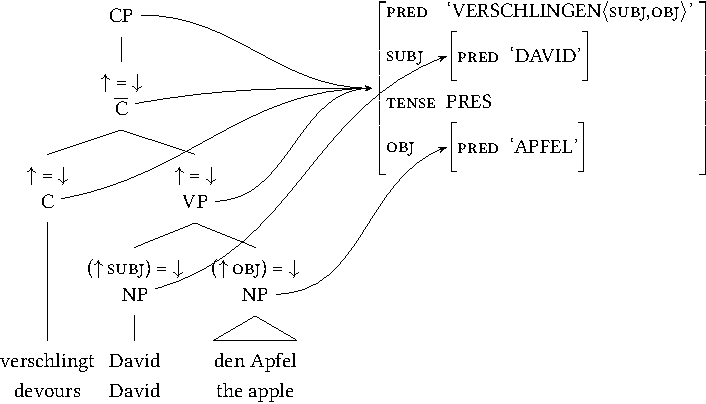
\includegraphics{Figures/verschlingt-david-den-apfel-lfg-lsp-crop}
}
\caption{\label{Abb-Verbstellung-LFG}Analysis of verb placement following \citet[\page 41]{Berman2003a}}
\end{figure}%

{\interfootnotelinepenalty=10%
\noindent
After what we learned about phrase structure rules in Chapters~\ref{Kapitel-PSG} and~\ref{Kapitel-GPSG}, it may seem strange to allow VPs without V. This is not a problem in LFG,
however, since for the analysis of a given sentence, it only has to be ensured that all the necessary parts (and only these) are present. This is ensured by the constraints on 
completeness\is{completeness} and coherence\is{coherence}. Where exactly the information comes from is not important. In Figure~\ref{Abb-Verbstellung-LFG}, the verb information
does not come from the VP, but rather from the C node.
C$'$ is licensed by a special rule:
\ea
\phraserule{C$'$}{
\rulenode{C\\* \up~=~\down}
\rulenode{VP\\*\up~=~\down}}
\z
In LFG rules, there is normally only one element annotated with `\up~=~\down', namely the head. In (\mex{0}), there are two such elements, which is why both equally contribute to the
f"=structure of the mother. The head domain of V has been extended to C. The information about \lfgsubj and \lfgobj comes from the VP and the information about \pred from C.%
\is{head domain!extended|)}\is{verb"=final language}

\section{Local reordering}
\label{Abschnitt-LFG-Umstellung}

Two\is{constituent order} possibilities for treating local reordering have been discussed in the literature:\footnote{%
  \citet[\page 20--21]{Kaplan95a} shows how one can write grammars in the ID/LP format\is{ID/LP grammar} in LFG. A GPSG"=like\indexgpsg analysis of German constituent
  order has not been proposed in the LFG framework.%
}
\begin{itemize}
\item movement of arguments from a base configuration as in GB\indexgb (see \citealp{Choi99a-u})
\item direct licensing by phrase structure rules (see Berman \citeyear[Section~2.1.3.1]{Berman96a-u}; \citeyear{Berman2003a})
\end{itemize}

\noindent
If one assumes that traces are relevant for the semantic interpretation of a given structure, then the first option has the same problems as movement"=based GB analyses.
These have already been discussed in Section~\ref{sec-GB-lokale-Umstellung}.

In what follows, I will present the analysis proposed by  \citet[Section~2.1.3]{Berman96a-u} in a
somewhat simplified form. Case and grammatical functions of verbal arguments are determined
in the lexicon \citep[\page 22]{Berman96a-u}. (\mex{1}) shows the lexical entry for the verb \emph{verschlingen} `devour':\footnote{%
The four cases in German can be represented using two binary features ({\small GOV}, {\small OBL}) \citep[\page 22]{Berman96a-u}. Nominative corresponds to {\small GOV}$-$ and
  {\small OBL}$-$ and accusative to {\small GOV}$+$ and {\small OBL}$-$. This kind of encoding allows one to leave case partially underspecified. If one does not provided a value
  for {\small GOV}, then an element with {\small OBL}$-$  is compatible with both nominative and accusative. Since this underspecification is not needed in the following discussion,
  I will omit this feature decomposition and insert the case values directly.
}$^,$\footnote{%
	Alternative analyses derive the grammatical function of an NP from its case (\citealp[\page 37]{Berman2003a} for German; \citealp[\page 187, \page 201]{Bresnan2001a} for German and Russian\il{Russian}).

\ea
\label{Kasus-Implikation-Berman}
\upshape      (\downsp \case) = \mdacc{} $\Rightarrow$ (\upsp \lfgobj) = \down{}
\z

\noindent
  \citet[Section~2.1]{Karttunen89a-u} makes a similar suggestion for Finnish\il{Finnish} in the framework of Categorial Grammar\indexcxg.
  Such analyses are not entirely unproblematic as case cannot always be reliably paired with grammatical functions. In German, as well as temporal
  accusatives (ii.a), there are also verbs with two accusative objects (ii.b--c) and predicative accusatives (ii.d).

\eal
\ex 
\gll Er arbeitete den ganzen Tag.\\
	 he worked the.\acc{} whole.\acc{} day\\
\ex 
\gll Er lehrte ihn den Ententanz.\\
	 he taught him.\acc{} the.\acc{} duck.dance\\
\ex 
\gll Das kostet ihn einen Taler.\\
	 that costs him.\acc{} a.\acc{} taler\\
\ex 
\gll Sie nannte ihn einen Lügner.\\
	 she called him.\acc{} a.\acc{} liar\\
\zl
All of these accusatives can occur in long"=distance dependencies (see Section~\ref{Abschnitt-NLA-LFG}):

\ea
\gll Wen glaubst du, dass ich getroffen habe.\\
	 who believe you that I met have\\
\glt `Who do you think I met?'
\z

\noindent
\emph{wen} is not the object of \emph{glauben} `believe' and as such cannot be included in the
f"=structure of \emph{glauben} `believe'. One would have to reformulate the implication in
(i) as a disjunction of all possible grammatical functions of the accusative and in addition account
for the fact that accusatives can come from a more deeply embedded f"=structure.

\citet[\page 202]{Bresnan2001a} assumes that nonlocal dependencies crossing a clause involve a gap
in German. With such a gap one can assume that case is only assigned locally within the verbal
projection. In any case one would have to distinguish several types of frontings in German and the
specification of case/grammatical function interaction would be much more complicate than (\ref{Kasus-Implikation-Berman}).%
%Stellt sich aber immer noch die Frage, ob man weiß, was der Trace für kategoriale
%Eigenschaften hat. Man findet den inside out und sagt dann OK, Deine Eigenschaften kenne ich jetzt
%und desahlb muss dann Deine grammatisceh Funktion hier Objekt sein. Oder?
%
% Traces seem to help here, but then there should be a connection between the fronted XP and the
% trace. Is there any connection other than the f-structure? The implication should not apply to the
% prefield. Lots of additional stipulations seem to be needed.
% Bresnan 2001:188 says that Russian does not have traces since it morphologically marks its dependends.
}
\ea
\label{le-verschlingen}
\catlexentry{verschlingt}{V}{(\up\ \pred) = {\small `VERSCHLINGEN\arglist{\lfgsubj, \lfgobj}'}\\*
                             (\up\ \lfgsubj{} {\small AGR CAS}) = NOM\\*
                             (\up\ \lfgobj{} {\small AGR CAS}) = ACC\\*
                             (\up\ \lfgtense) = \small PRES}
\z

%\addlines
\largerpage
\noindent
Berman proposes an analysis that does not combine the verb with all its arguments and adjuncts at
the same time, as was the case in GPSG\indexgpsg. Instead, she chooses the other extreme and assumes
that the verb is not combined with an adjunct or an argument, but rather forms a VP directly. The rule for this is shown in (\mex{1}):
\ea
\label{LFG-v-vp}
\phraserule{VP}{
\rulenode{(V)\\* \up~=~\down}}
\z
At first sight, this may seem odd since a V such as \emph{verschlingen} `devour' does not have the same distribution as a verb with its arguments. However, one should recall that the
constraints pertaining to coherence and completeness of f"=structures play an important role so that
the theory does not make incorrect predictions.
}% footnote breaks

Since the verb can occur in initial position, it is marked as optional in the rule in (\mex{0}) (see Section~\ref{Abschnitt-Verbstellung-LFG}).

The following rule can be used additionally to combine the verb with its subject or object.
\ea
\label{lfg-vp-regel}
\phraserule{VP}{
\rulenode{NP\\* (\upsp \lfgsubj|\lfgobj|\objtheta) = \down}
\rulenode{VP\\* \up~=~\down}}
\z
The `|'\is{$\vert$} here stands for a disjunction\is{disjunction}, that is, the NP can either be the subject or the object of the superordinate f"=structure. Since VP occurs both on the left
and right"=hand side of the rule in (\mex{0}), it can be applied multiple times.
The rule is not complete, however. For instance, one has to account for prepositional objects, for clausal
arguments, for adjectival arguments and for adjuncts. See footnote~\ref{fn-zp} on page~\pageref{fn-zp}.

\largerpage
Figure~\vref{Abb-SOV-LFG} shows the analysis for (\mex{1}a). 
\eal
\ex 
\gll {}[dass] David den Apfel verschlingt\\
      \spacebr{}that David the apple devours\\
\glt `that David is devouring the apple'
\ex 
\gll {}[dass] den Apfel David verschlingt\\
     \spacebr{}that the apple David devours\\
\zl
\begin{figure}
\centerline{%
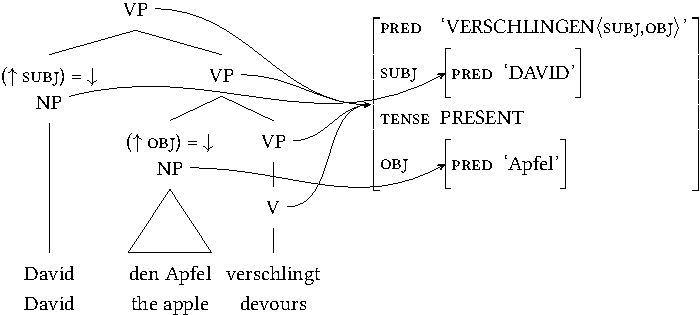
\includegraphics{Figures/david-den-apfel-verschlingt-lfg-lsp-crop}
}
\caption{\label{Abb-SOV-LFG}Analysis of SOV order following \citet{Berman96a-u}}
\end{figure}%
The analysis of (\mex{0}b) is shown in Figure~\vref{Abb-OSV-LFG}.
\begin{figure}
\centerline{%
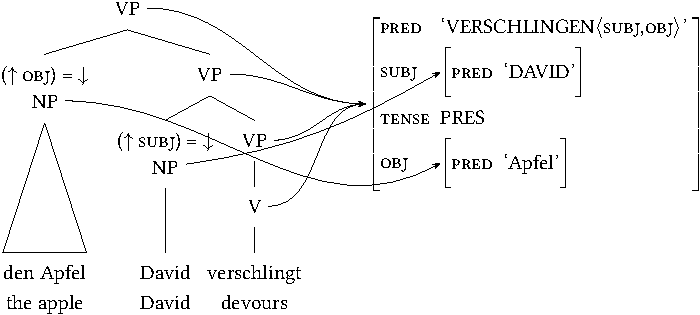
\includegraphics{Figures/den-apfel-david-verschlingt-lfg-lsp-crop}
}
\caption{\label{Abb-OSV-LFG}Analysis of OSV order following \citet{Berman96a-u}}
\end{figure}%
The analysis of (\mex{0}b) differs from the one of (\mex{0}a) only in the order of the replacement
of the NP node by the subject or object.\todostefan{fix the arrows, should not cross SUBJ and OBJ}

One further fact must be discussed: in the rule (\ref{LFG-v-vp}), the verb is optional. If it is
omitted, the VP is empty. In this way, the VP rule in (\ref{lfg-vp-regel}) can have an empty VP on
the right"=hand side of the rule. This VP is also simply
omitted even though the VP symbol in the right-hand side of rule (\ref{lfg-vp-regel})  is not marked as optional.
That is, the corresponding symbol then also becomes optional as a result of taking the rest of the grammar into consideration as well as possible interactions with
other rules.\is{constituent order|)}  

\section{Long"=distance dependencies and functional uncertainty}
\label{Abschnitt-NLA-LFG}

We\is{long"=distance dependency|(} have seen that LFG can explain phenomena such as passivization, local reordering as well as verb placement without transformations.
In Chapter~\ref{Kapitel-GPSG} on GPSG, we already saw that the development of a transformation"=less analysis for long"=distance dependencies constitutes a real achievement.
In LFG, \citet{KZ89a} proposed another transformation"=less analysis of long"=distance dependencies, which we will consider in further detail in what follows.

%\addlines[-1]
In example (\mex{1}), the displaced constituent \emph{Chris} is characterized by two functions:
\ea
\label{ex-Chris-we-think}
Chris, we think that David saw.
\z
For one, it has an argument function which is normally realized in a different position (the \lfgobj function of \emph{saw} in the above example) and additionally it has a discourse function:
a certain emphasis of the information"=structural status in this construction (\textsc{topic} in the matrix clause).
In LFG, \textsc{topic} and \textsc{focus} are assumed to be grammaticalized discourse functions (furthermore, \textsc{subj} is classified as the default discourse function). Only
grammaticalized discourse functions are represented on the level of f"=structure, that is, those
that are created by a fixed syntactic mechanism and that interact with the rest of the syntax. 

Unlike argument functions, the discourse functions  \textsc{topic}\isfeat{topic}\is{topic} and
\textsc{focus}\isfeat{focus}\is{focus} are not lexically subcategorized and are therefore not subject to the completeness\is{completeness} and 
coherence\is{coherence} conditions. The values of discourse function features like \textsc{topic}
and \textsc{focus} are identified with an f"=structure that bears an argument function.  (\mex{1})  
gives the f"=structure for the sentence in (\ref{ex-Chris-we-think}):

\ea
\lfgms{ pred & `THINK\sliste{ \lfgsubj, comp }' \\
        topic & \rnode{topic}{\lfgms{ pred & `CHRIS' \\
                                   }}\\[4mm]
        subj & \lfgms{ pred & `pro'\\
                     }\\
        comp & \lfgms{ pred & `SEE\sliste{ \lfgsubj, \lfgobj }'\\
                       subj & \lfgms{ pred & `DAVID' \\
                                    }\\
                       obj  & \rnode{obj}{}\\
                     }\\
      }
% todo \nodecurve[r]{topic}[r]{obj}{15em}
\nccurve[ncurv=2.2]{topic}{obj}
\z

\noindent
The connecting line means that the value of \textsc{topic} is identical to the value of
\textsc{comp$|$obj}. In Chapter~\ref{chap-feature-descriptions} on feature descriptions, I used boxes for structure sharing
rather than connecting lines, since boxes are more common across frameworks.
It is possible to formulate the structure sharing in (\mex{0}) as an f-structure constraint as in (\mex{1}):
\ea
\label{Topic-Comp-Obj}
(\upsp  \textsc{topic}) = (\upsp \textsc{comp obj})
\z

\noindent
Fronting operations such as (\ref{ex-Chris-we-think}) are possible from various levels of embedding:
for instance, (\mex{1}a) shows an example with less embedding.
The object is located in the same f"=structure as the topic. However, the object in (\ref{ex-Chris-we-think}) comes from a clause embedded under \emph{think}.

The f"=structure corresponding to (\mex{1}a) is given in (\mex{1}b):

\eal
\ex Chris, we saw.
\ex 
\lfgms{ pred & `SEE\sliste{ \lfgsubj, \lfgobj }' \\
        topic & \rnode{topic}{\lfgms{ pred & `CHRIS' \\
                                   }}\\[4mm]
        subj & \lfgms{ pred & `pro'\\
                     }\\
        obj  & \rnode{obj}{}\\
      }
% todo \nodecurve[r]{topic}[r]{obj}{15em}
\nccurve[nodesepA=1pt,ncurv=2.2]{topic}{obj}
\zl

\noindent
The identity restriction for \topic{} and object can be formulated in this case as in (\mex{1}):

\ea
\label{Topic-Obj}
(\upsp  \textsc{topic}) = (\upsp \textsc{obj})
\z

\noindent
Example (\mex{1}a) shows a case of even deeper embedding than in (\ref{ex-Chris-we-think}) and
(\mex{1}b,c) show the corresponding f"=structure and the respective restriction.

\eal
\ex Chris, we think Anna claims that David saw.
\ex 
\lfgms{ pred & `THINK\sliste{ \lfgsubj, comp }' \\
        topic & \rnode{topic}{\lfgms{ pred & `CHRIS' \\
                                   }}\\[4mm]
        subj & \lfgms{ pred & `pro'\\
                     }\\
        comp & \lfgms{ pred & `CLAIM\sliste{ \lfgsubj, comp }\\
                       subj & \lfgms{ pred & `ANNA' \\
                                   }\\
                       comp & \lfgms{ pred & `SEE\sliste{ \lfgsubj, \lfgobj }\\
                                      subj & \lfgms{ pred & `DAVID' \\
                                                   }\\
                                      obj  & \rnode{obj}{}\\
                                    }\\
                     }\\
      }
% todo \nodecurve[r]{topic}[r]{obj}{15em}%
\nccurve[ncurv=2.2]{topic}{obj}
\ex\label{Topic-Comp-Comp-Obj}
(\upsp  \textsc{topic}) = (\upsp \textsc{comp comp obj})
\zl


\noindent
The restrictions in (\ref{Topic-Comp-Obj}), (\ref{Topic-Obj}) and
(\ref{Topic-Comp-Comp-Obj}) are c"=structure constraints. The combination of a c"=structure with (\ref{Topic-Comp-Obj}) is given in (\mex{1}):
\ea
\begin{tabular}[t]{@{}ccc@{~=~}lc@{}}
CP & $\rightarrow$ & \multicolumn{2}{l}{\hspaceThis{(\upsp \textsc{topic})}XP} & C$'$ \\
 & &  (\upsp \textsc{topic}) & \down & \up~=~\down \\
 & &  (\upsp \textsc{topic}) & (\upsp \textsc{comp obj})\\
\end{tabular}
\z
\addlines
(\mex{0}) states that the first constituent contributes to the \textsc{topic} value in the f"=structure of the mother and furthermore that this topic value has to be
identical to that of the object in the complement clause. We have also seen examples of other embeddings of various depths. We therefore need restrictions
of the following kind as in (\mex{1}): 
\eal
\ex (\upsp  \textsc{topic}) = (\upsp \textsc{obj})
\ex (\upsp  \textsc{topic}) = (\upsp \textsc{comp obj})
\ex (\upsp  \textsc{topic}) = (\upsp \textsc{comp comp obj})
\ex \ldots
\zl
The generalization emerging from these equations is given in (\mex{1}):
\ea
(\upsp  \textsc{topic}) = (\upsp \textsc{comp* obj})
\z

\noindent
Here, `*'\is{*} stands for an unrestricted number of occurrences of \mbox{\small COMP}. This means of leaving the possible identification of discourse and grammatical function open is known
as \emph{functional uncertainty}\is{functional uncertainty}, see \citew{KZ89a}.

As was shown in the discussion of examples (\ref{bsp-fronted-focus}) and (\ref{bsp-fronted-topic}) on
page~\pageref{bsp-fronted-focus}, it is not the case that only a \textsc{topic} can be placed in the specifier position of CP in English as \focus can occur there too.
One can use disjunctions in LFG equations and express the corresponding condition as follows:

\ea
(\upsp  \textsc{topic$|$focus}) = (\upsp \textsc{comp* obj})
\z
One can introduce a special symbol for \textsc{topic$|$focus}, which stands for a disjunction of discourse functions: \textsc{df}\isfeat{df}.
(\mex{0}) can then be abbreviated as in (\mex{1}):

\ea
(\upsp  \textsc{df}) = (\upsp \textsc{comp* obj})
\z

\noindent
The final version of the c"=structure rule for fronting in English will therefore have the form of
(\mex{1}):\footnote{%
  Note that the two disjunctions that are abbreviated by the respective occurrences of \textsc{df}
  are independent in principle. This is unwanted. We want to talk about either a topic or a focus
  not about a topic and a focus in the mother f-structure. So additional machinery is needed to
  ensure that both occurrences of \textsc{df} refer to the same discourse function.
}
\ea
\begin{tabular}[t]{@{}ccc@{~=~}lc@{}}
CP & $\rightarrow$ & \multicolumn{2}{l}{\hspaceThis{(\upsp \textsc{df})}XP} & C$'$ \\
 & &  (\upsp \textsc{df}) & \down & \up~=~\down \\
 & &  (\upsp \textsc{df}) & (\upsp \textsc{comp* obj})\\
\end{tabular}
\z
In German, as well as objects, nearly any other constituent (\eg subjects, sentential complements, adjuncts) can be fronted. The c"=structure rule for
this is shown in
(\mex{1}):\footnote{\label{fn-zp}%
  \citet{Berman96a-u} uses the symbol ZP for symbols in the prefield rather than XP in (\mex{1}). She formulates various phrase structure rules for ZPs, which replace ZP
  with NP, PP, AP and various adjuncts. Following Berman, ZPs can also be combined with the verb in the middle field. For reasons of exposition, I refrained from using 
  ZP symbols in the formulation of the VP rule (\ref{lfg-vp-regel}) in Section~\ref{Abschnitt-LFG-Umstellung} and instead used NP directly.
}
\ea
\begin{tabular}[t]{@{}ccc@{~=~}lc@{}}
CP & $\rightarrow$ & \multicolumn{2}{l}{\hspaceThis{(\upsp \textsc{df})}XP} & C$'$ \\
 & &  (\upsp \textsc{df}) & \down & \up~=~\down \\
 & &  (\upsp \textsc{df}) & (\upsp \textsc{comp* gf})\\
\end{tabular}
\z
Here, \textsc{gf} is an abbreviation for a disjunction of grammatical functions which can occur in the prefield.
\is{long"=distance dependency|)}



\section{Summary and classification}

LFG is a constraint"=based theory and utilizes feature descriptions and PSG rules. Grammatical functions are treated
as primitives of the theory, which sets LFG apart from most of the other theories covered in this book. They are not defined structurally (as in GB). LFG is a lexicalist theory. Like GPSG, LFG can do without transformations. Processes affecting
argument structure such as passivization are analyzed by means of lexical rules. Whereas GPSG treated long"=distance dependencies using the percolation of information
in trees, LFG uses functional uncertainty: a part of the f"=structure is identified with another
f"=structure that can be embedded to an arbitrary depth. Coherence\is{coherence} and completeness\is{completeness}
ensure that the long"=distance dependency can be correctly resolved, that is, it ensures that a fronted object is not assigned to an f"=structure which already contains an object or one
in which no object may occur.

While LFG does contain a phrase"=structural component, this plays a significantly less important role compared to other models of grammar. There are rules in which all constituents are
optional and it has even been proposed for some languages that there are rules where the part of speech of the constituents is not specified (see Section~\ref{sec-Diskussion-X-Bar}).
In these kinds of grammars, f"=structure, coherence and completeness work together to ensure that the grammar only allows well"=formed structures.

LFG differs from other theories such as \hpsg and variants of \cxg in that feature structures are untyped. Generalizations can therefore not be represented in type hierarchies. 
Until a few years ago, the hierarchical organization of knowledge in inheritance hierarchies\is{inheritance} did not form part of theoretical analyses. In computer implementations,
there were macros\is{macro} but these were viewed as abbreviations without any theoretical status. It is possible to organize macros into hierarchies and macros were discussed explicitly
in \citew*{DKK2004a} with reference to capturing linguistic generalizations. \citet*{ADT2008a} suggest using macros not only for the organization of lexical items but also for
capturing generalizations regarding c"=structure annotations. Because of these developments, there was a greater convergence between LFG and other theories such as HPSG and CxG.

\citet{Williams84a} compares analyses in LFG with GB. He shows that many analyses are in fact transferable: the function that f"=structure has in LFG is handled by the
Theta"=Criterion\is{theta-theory@$\theta$-Theory}\is{theta-criterion@Theta"=Criterion} and Case Theory\is{case}\is{Case Theory} in GB. LFG can explicitly differentiate between subjects and non"=subjects. In GB, on the other hand,
a clear distinction is made between external\is{argument!external} and internal\is{argument!internal} arguments (see \citealp[Section~1.2]{Williams84a}). In some variants of GB, as well as
in HPSG\indexhpsg and CxG\indexcxg, the argument with subject properties (if there is one) is marked explicitly \citep{Haider86,HM94a,Mueller2003e,MR2001a}. This special argument
is referred to as the \emph{designated argument}\is{argument!designated}. In infinitival constructions, subjects are often not expressed inside the infinitival phrase. Nevertheless, 
the unexpressed subject is usually coreferential with an argument of the matrix verb:

\eal
\ex 
\gll Er versucht, [das Buch zu lesen].\\
	 he tries \spacebr{}the book to read\\
\glt `He is trying to read the book.'
\ex 
\gll Er zwingt ihn, [das Buch zu lesen].\\
	 he forces him \spacebr{}the book to read\\
\glt `He is forcing him to read the book.´
\zl 
This is a fact that every theory needs to be able to capture, that is, every theory must be able to differentiate between subjects and non"=subjects.

For a comparison of GB/Minimalism and LFG/HPSG, see \citew{Kuhn2007a}.


\section*{Comprehension questions}

\begin{enumerate}
\item What do the terms \emph{coherence} and \emph{completeness} mean?
\item What are extended head domains?
\item What does lexical integrity mean?
\end{enumerate}

\section*{Exercises}

\begin{enumerate}
\item Give the lexical entry for \emph{kannte} `knew'.
\item How could one analyze the following sentence?
\ea
\gll Den Apfel verschlingt David.\\
	 the apple devours David\\
\glt `David devours the apple.'
\z
Provide the necessary c"=structure rules. What kind of f"=structure is licensed?
Draw a syntactic tree with corresponding references to the f"=structure. For fronted constituents,
simply write NP rather than expanding the XP node.
The c"=structure rule for the NP can also be omitted and a triangle can be drawn in the tree.
\end{enumerate}


\section*{Further reading}


Section~\ref{Abschnitt-Format-LFG} was based extensively on the textbook and introductory article of \citet{Dalrymple2001a-u,Dalrymple2006a}. Additionally, I have drawn from
teaching materials of Jonas Kuhn from 2007. \citew{Bresnan2001a} is a comprehensive textbook in English for the advanced reader. Some of the more in"=depth analyses of
German in LFG are \citew{Berman96a-u,Berman2003a}.  \citew{SdA2016a-u} is an introduction to LFG that uses French\il{French} examples. The authors demonstrate how the XLE system can be used for the development of a
French\il{French} LFG grammar. The textbook also discusses the Finite State Morphology component that comes
with the XLE system.

\citet{Levelt89a} developed a model of language production based on LFG.
 \citet{Pinker84a-u} -- one of the best"=known researchers on language acquisition -- used LFG as the model for his theory of acquisition. For another theory on first and second
 language acquisition that uses LFG, see \citew{Pienemann2005a}. 



%      <!-- Local IspellDict: en_US-w_accents -->



%% Bresnan:

%% The internal structure of a language represents the meaningful grammatical relations of sentences (how their syntactic functions are associated with semantic predicate argument relations); this structure is determined by generalizations about case government, pronominal binding, and agreement relations among the predicators and arguments of a sentence. The principle of universality states that internal structures are largely invariant across languages. The formal model of internal structure in LFG is the f-structure, 'functional structure'. (1996:34 f.)

%% As we have already seen in Ch. 3, the principles of completeness and coherence require full
%% representation of grammatical relations in f-structure. Full representation might be thought of
%% as a universal iconicity requirement between syntax and semantics at f-structure. (1996:83) 


% Dyvik dazu: http://folk.uib.no/hfohd/LFG99/LFG99Dyvik.html

%% -*- coding:utf-8 -*-

\chapter{Categorial Grammar}
\label{Kapitel-CG}\label{chap-CG}

Categorial Grammar\is{Categorial Grammar (CG)|(} is the second oldest of the approaches discussed in this book. It was developed in the 30s by the Polish logician
\href{http://en.wikipedia.org/wiki/Kazimierz_Ajdukiewicz}{Kazimierz Ajdukiewicz}
\citep{Ajdukiewicz35a-u}. Since
syntactic and semantic descriptions are tightly connected and all syntactic combinations correspond
to semantic ones, Categorial Grammar is popular amongst logicians and semanticists.
Some stellar works in the field of semantics are those of Richard Montague \citeyearpar{Montague74a-u}.

Other important works come from David Dowty in Columbus, Ohio \citeyearpar{Dowty79a}, Michael
Moortgat in Utrecht \citeyearpar{Moortgat89a-u}, Glyn Morrill in Barcelona
\citeyearpar{Morrill94a-u}, Bob Carpenter in New York \citeyearpar{Carpenter98a-u} and Mark Steedman
in Edinburgh \citeyearpar{Steedman91a,Steedman97a,Steedman2000a-u}. A large fragment for German using Montague Grammar has been developed by \citew{Stechow79}.
The 2569"=page grammar of the \emph{Institut für Deutsche Sprache} in Mannheim \citep*{IDS97} contains Categorial Grammar analyses in the relevant chapters.
\citet{Fanselow81a-u} worked on morphology in the framework of Montague Grammar.  \citet{Uszkoreit86d},
\citet{Karttunen86a,Karttunen89a-u} and \citet*{CKZ88a} developed combinations of unification"=based approaches and Categorial Grammar.

The basic operations for combining linguistic objects are rather simple and well"=understood, so
that it is no surprise that there are many systems for the development and processing of Categorial Grammars
\citep*{YK90a-u,Carpenter1994a-u,BvN94a-u,Llore1995a-u,Koenig99a-u,Moot2002a-u,WB2003a-u,BCPW2007a,Morrill2012a}. An
important contribution has been made by Mark Steedman's group (see for instance \citealp*{CHS2002a-u,CC2007a-u}).

%% , aber auch in Deutschland gab und
%% gibt es computerlinguistische Gruppen, die in diesem theoretischen Rahmen arbeiten
%% \citep*{Uszkoreit86d,Koenig99a-u,VHE2003a}.
%% MCGTOOLS: Llore1995a-u
Implemented fragments exist for the following languages:
\begin{itemize}
\item German \citep*{Uszkoreit86d,Koenig99a-u,VHE2003a,VTBS2011a}
\item English\il{English} \citep{Villavicencio2002a,Baldridge2002a-u,Beavers2002a-u,Beavers2004a-u}
% CMZ86a ist ein Report, den gibt es aber nirgends
\item Finish\il{Finnish} \citep{Karttunen89a-u}
\item French\il{French} \citep*{BBCG87a-u}
\item Dutch\il{Dutch} \citep{BvN94a-u,Baldridge2002a-u}
\item Tagalog\il{Tagalog} \citep{Baldridge2002a-u}
\item Turkish\il{Turkish} \citep{Hoffmann95a-u,Baldridge2002a-u}
\end{itemize}
In addition, \citet*[\page 15]{BCPW2007a} mention an implementation for Classical Arabic\il{Arabic}.

Some of the systems for the processing of Categorial Grammars have been augmented by probabilistic\is{statistics}
components, so that the processing is robust \citep*{OB97a,CHS2002a-u}. Some systems can derive lexical items from corpora and \citet{Briscoe2000a} and \citet{Villavicencio2002a} use statistical
information in their UG"=based\is{Universal Grammar (UG)} language acquisition models.\is{language acquisition}


%      <!-- Local IspellDict: en_US-w_accents -->


\section{General remarks on the representational format}


\subsection{Representation of valence information}
\label{sec-forward-backward-application}

In\is{valence|(} Categorial Grammar, complex categories replace the \subcatf that is used in GPSG\indexgpsg to ensure that a head can only be used with
suitable grammatical rules. Simple phrase structure rules\is{phrase structure grammar} can be replaced with complex categories as follows:\is{/|(} 

\ea
\label{LE-CG}
\begin{tabular}[t]{@{}l@{\hspace{1cm}}l}
Rule                              & Category~in~the~lexicon\\
vp $\to$ v(ditrans) np~np         & (vp/np)/np  \\
vp $\to$ v(trans) np              & vp/np  \\
vp $\to$ v(np\_and\_pp) np~pp(to) & (vp/pp)/np  \\
\end{tabular}
\z
vp/np stands for something that needs an np in order for it to form a vp.

In Categorial Grammar, there are only a few very abstract rules. One of these is forward application, also referred to as the multiplication rule:
\ea
\label{vorwaertsapplikation}\label{forward-application}
forward application\is{forward application}:\\
X/Y $*$ Y = X
\z
This rule combines an X looking for a Y with a Y and requires that Y occurs to the right of X/Y.
The result of this combination is an X that no longer requires a Y. X/Y is called the \emph{functor}\is{functor}
and Y is the \emph{argument}\is{argument} of the functor.

Valence is encoded only once in Categorial Grammar, as in \gbt, in the lexicon. In GPSG\indexgpsg, valence information was present in grammatical rules
and in the \subcatf of the lexical entry.

Figure~\vref{abb-cg-transitives-Verb} shows how a lexical entry for a transitive verb is combined
with its object.\todostefan{Die Linien sind zu hoch im vergleich zum $<$}
\begin{figure}
\centerline{%
\deriv{2}{
%\begin{tabular}{@{}cc@{}}
chased       & Mary\\
%\uline{1}    & \uline{1} \\
\hr & \hr\\
vp/np   & np\\
\multicolumn{2}{@{}c@{}}{\forwardapp} \\
\multicolumn{2}{@{}c@{}}{vp}\\
%\cgmc<2->{2}{vp}\\
%\end{tabular}
}
}
\caption{\label{abb-cg-transitives-Verb}Combination of a verb and its object (preliminary)}
\end{figure}%
A derivation in CG is basically a binary branching tree, it is however mostly represented as follows:
an arrow under a pair of categories indicates that these have been combined via a combinatorial rule. The direction of this arrow indicates the direction
of this combination. The result is given beneath the arrow. Figure~\vref{Abb-CG-als-Baum} shows the tree corresponding to Figure~\ref{abb-cg-transitives-Verb}.
\begin{figure}
\centerline{%
\begin{forest}
sn edges
[vp
	[vp/np
		[chased]]
	[np
		[Mary]]]
\end{forest}
}
\caption{\label{Abb-CG-als-Baum}Derivation in Figure~\ref{abb-cg-transitives-Verb} as a tree diagram}
\end{figure}%
One usually assumes left associativity\is{left associativity}
for `/', that is, (vp/pp)/np = vp/pp/np.\is{/|)}

If we look at the lexical entries in (\ref{LE-CG}), it becomes apparent that the category v does not appear. The lexicon only determines what the product of
combination of a lexical entry with its arguments is. The symbol for vp can also be eliminated: an (English) vp is something that requires an NP to its left in
order to form a complete sentence. This\is{$\backslash$|(} can be represented as s$\backslash$np.
Using the rule for backward application, it is possible to compute derivations such as the one in Figure~\vref{abb-the-cat-chased-Mary}.\is{valence|)}
\ea
Backward application\is{backward application}:\\
Y $*$ X$\backslash$Y = X 
\z

\begin{figure}
\centerline{%
\deriv{4}{
the  & cat & chased         & Mary\\
\hr  & \hr & \hr            & \hr \\
np/n & n   & (s\bs np)/np   & np\\
\multicolumn{2}{@{}c}{\forwardapp} & \multicolumn{2}{c@{}}{\forwardapp}\\
\multicolumn{2}{c}{{np}}             & \multicolumn{2}{c@{}}{{s\bs np}}\\
\multicolumn{4}{@{}c@{}}{\backwardapp}\\
\multicolumn{4}{c@{}}{{s}}\\
}}
\caption{\label{abb-the-cat-chased-Mary}Analysis of a sentence with a transitive verb}
\end{figure}%

\noindent
In Categorial Grammar, there is no explicit difference made between phrases and words: an intransitive verb is described in the same way as a verb phrase with an
object:  s$\backslash$np. In the same way, proper nouns are complete noun phrases, which are assigned the symbol np.\is{$\backslash$|)}

\subsection{Semantics}

As already mentioned, Categorial Grammar is particularly popular among semanticists as syntactic
combinations always result in parallel semantic combinations and even for complex combinations such
as those we will discuss in more detail in the following sections, there is a precise definition of
meaning composition.
In the following, we will take a closer look at the representational format discussed in \citet[Section~2.1.2]{Steedman97a}.

Steedman proposes the following lexical entry for the verb \emph{eats}:\footnote{
 I have adapted his notation to correspond to the one used in this book.
}
\ea
eats := (s: \relation{eat}(x, y)\bs np\sub{3S}:x)/np:y
\z
In (\mex{0}), the meaning of each category is given after the colon. Since nothing is known about
the meaning of the arguments in the lexical entry of \emph{eat},
the meaning is represented by the variables $x$ and $y$. When the verb combines with an NP, the denotation of the NP is inserted. An example is given in (\mex{1}):\footnote{
The assumption that \emph{apples} means \relation{apples} and not \relation{apples}(z) minus the quantifier contribution is a simplification here.
}
\ea
\deriv{2}{
(s: eat'(x, y)\bs np_{3S}:x)/np:y & np: apples'\\
\multicolumn{2}{@{}c@{}}{\forwardapp}\\
s: eat'(x, apples')\bs np_{3S}:x\\
}
\z
When combining a functor with an argument, it must be ensured that the argument fits the functor, that is, it must be unifiable\is{unification} with it
(for more on unification see Section~\ref{sec-unification}). The unification of np:y with np: \relation{apples} results in np: \relation{apples} since \relation{apples}
is more specific than the variable y. Apart from its occurrence in the term np:y, y occurs in the description of the verb in another position (s:
\relation{eat}(x, y)\bs np\sub{3S}:x) and therefore also receives the value \relation{apples}
there. Thus, the result of this combination is s: \relation{eat}(x, \relation{apples})\bs np$_{3S}$:x 
as shown in (\mex{0}).

Steedman notes that this notation becomes less readable with more complex derivations and instead uses the more standard $\lambda$"=notation:
\ea
eats := (s\bs np\sub{3S})/np: $\lambda y.\lambda x.\relation{eat}(x, y)$
\z
Lambdas are used to allow access to open positions in complex semantic representations (see Section~\ref{sec-PSG-Semantik}). A semantic representation such as
$\lambda
y.\lambda x.\relation{eat}(x, y)$ can be combined with the representation of \emph{apples} by
removing the first lambda expression and inserting the denotation of \emph{apples}
in all the positions where the corresponding variable (in this case, y) appears (see Section~\ref{sec-PSG-Semantik} for more on this point):
\ea
$\lambda y.\lambda x.eat'(x, y)$ \relation{apples}\\
$\lambda x.eat'(x, apples')$
\z
This removal of lambda expressions is called $\beta$"=reduction\is{beta"=reduction@$\beta$"=reduction}\label{Seite-beta-Reduktion}.

If we use the notation in (\mex{-1}), the combinatorial rules must be modified as follows:
\ea
\begin{tabular}[t]{@{}l@{ * }l@{ = }c}
X/Y:f & Y:a & X: f a\\
Y:a & X\bs Y:f & X: f a\\ 
\end{tabular}
\z
In such rules, the semantic contribution of the argument (a) is written after the semantic denotation of the functor (f). The open positions in the denotation of
the functor are represented using lambdas. The argument can be combined with the first lambda expression using $\beta$-reduction.

Figure~\vref{Abb-Semantik-CG} shows the derivation of a simple sentence with a transitive verb.
\begin{figure}
\centerline{%
\deriv{3}{
Jacob & eats         & apples\\
\hr & \hr          & \hr \\
np:\relation{jacob}  & (s\bs np)/np: \lambda y.\lambda x.eat'(x, y) & np:apples'\\
         & \multicolumn{2}{c@{}}{\forwardapp}\\
         & \multicolumn{2}{c@{}}{\begin{tabular}[t]{@{}l@{}l@{}}
                              s\bs np&: $\lambda y.\lambda x.eat'(x, y)\; apples'$\\
                                     &= $\lambda x.eat'(x, apples')$\\
                              \end{tabular}}\\
\multicolumn{3}{@{}c@{}}{\backwardapp}\\
\multicolumn{3}{c@{}}{\begin{tabular}[t]{@{}l@{}l@{}}
                    s&: $\lambda x.eat'(x, apples')\; jacob'$\\
                     &= $eat'(jacob', apples')$\\
                              \end{tabular}}\\
}}
\caption{\label{Abb-Semantik-CG}Meaning composition in Categorial Grammar}
\end{figure}%
After forward and backward application, $\beta$"=reduction is immediately applied.

\subsection{Adjuncts}

As\is{adjunct|(} noted in Section~\ref{sec-intro-arg-adj}, adjuncts are optional. In phrase
structure grammars, this can be captured for example by rules that have a certain element (for
instance a VP) on the left"=hand side of the rule and the same element and an adjunct on the
right"=hand side of the rule. Since the symbol on the left is the same as the one on the right, this rule can be
applied arbitrarily many times. (\mex{1}) shows some examples of this:
\eal
\ex VP $\to$ VP~PP
\ex Noun $\to$ Noun~PP
\zl
One can analyze an arbitrary amount of PPs following a VP or noun using these rules.

In Categorial Grammar, adjuncts have the following general form: X\bs X or X/X.
Adjectives are modifiers, which must occur before the noun. They have the category n/n.
Modifiers occurring after nouns (prepositional phrases and relative clauses) have the category
n\bs n instead.\footnote{
	In Categorial Grammar, there is no category symbol like \xbar for intermediate projections of
	\xbart. So rather than assuming \nbar/\nbar, CG uses n/n. See Exercise~\ref{ue-Xbar-CG}.
} For VP-modifiers, X is replaced by the symbol for the VP (s\bs np) and this yields the relatively complex expression (s\bs np)\bs (s\bs np).
Adverbials in English are VP"=modifiers and have this category. Prepositions that can be used in a PP modifying a verb require an NP in order to
form a complete PP and therefore have the category ((s\bs np)\bs (s\bs
np))/np. Figure~\vref{abb-CG-Adjunktion} gives an example of an adverb (\emph{quickly}) and a preposition (\emph{round}). 
%
\begin{figure}
\oneline{%
\deriv{9}{
The  & small & cat & chased       & Mary & quickly                & round                     & the & garden\\
\hr  & \hr   & \hr & \hr          & \hr  & \hr                    & \hr                       & \hr & \hr\\
np/n & n/n   & n   & (s\bs np)/np & np   & (s\bs np)\bs (s\bs np) & (s\bs np)\bs (s\bs np)/np & np/n & n\\
     & \multicolumn{2}{c}{\forwardapp} & \multicolumn{2}{c}{\forwardapp}\\
     & \multicolumn{2}{c}{n}           & \multicolumn{2}{c}{s\bs np}\\
\multicolumn{3}{@{}c}{\forwardapp}        & \multicolumn{3}{c}{\backwardapp}\\
\multicolumn{3}{@{}c}{np}                 & \multicolumn{3}{c}{s\bs np}\\
&&&&&&&\multicolumn{2}{c@{}}{\forwardapp}\\
&&&&&&&\multicolumn{2}{c@{}}{np}\\
&&&&&&\multicolumn{3}{c@{}}{\forwardapp}\\
&&&&&&\multicolumn{3}{c@{}}{(s\bs np)\bs (s\bs np)}\\
&&&\multicolumn{6}{c@{}}{\backwardapp}\\
&&&\multicolumn{6}{c@{}}{(s\bs np)}\\
\multicolumn{9}{@{}c@{}}{\backwardapp}\\
\multicolumn{9}{@{}c@{}}{s}\\
}}
\caption{\label{abb-CG-Adjunktion}Example of an analysis with adjuncts in Categorial Grammar}
\end{figure}%
Note that the result of the combination of \emph{round} and \emph{the garden} corresponds to the category of the adverb ((s\bs np)\bs (s\bs np)).
In \gbt, adverbs and prepositions were also placed into a single class (see page~\pageref{Seite-Adverbien-PP}). This overarching class was then divided into subclasses
based on the valence of the elements in question.
\is{adjunct|)}

\section{Passive}

In Categorial Grammar, the passive\is{passive|(} is analyzed by means of lexical rule (\citealp[\page412]{Dowty78a};
\citealp[Section~3.4]{Dowty2003a}). (\mex{1}) shows the rule in \citew[\page 49]{Dowty2003a}.
\ea
\label{Lexikonregel-Passiv-CG}
\begin{tabular}[t]{@{}ll@{~$\to$~}l@{}}
Syntax:   & $\alpha \in$ (s\bs np)/np & PST-PART($\alpha$) $\in$ PstP/np$_{by}$\\
Semantics: & $\alpha'$                 & $\lambda y\lambda x \alpha'(y) (x)$
\end{tabular}
\z
Here, PstP stands for past participle and np$_{by}$ is an abbreviation for a verb phrase modifier of
the form vp\bs vp or rather (s\bs np)\bs (s\bs np).
The rule says the following: if a word belongs to the set of words with the category (s\bs
np)/np, then the word with past participle morphology also belongs in the set of words with the category PstP/np$_{by}$.

(\mex{1}a) shows the lexical entry for the transitive verb \emph{touch} and (\mex{1}b) the result of rule application:
\eal
\ex touch:   (s\bs np)/np
\ex touched: PstP/np$_{by}$ 
\zl
The auxiliary \emph{was} has the category (s\bs np)/PstP and the preposition \emph{by} has the category  np$_{by}$/np, or its unabbreviated form ((s\bs np)\bs (s\bs np))/np.
In this way, (\mex{1}) can be analyzed as in Figure~\vref{abb-CG-Passiv}.
\ea
John was touched by Mary.
\z
\begin{figure}
\centerline{%
\deriv{5}{%
John & was            & touched      & by         & Mary.\\
\hr  & \hr            & \hr_{\mathrm{LR}}  & \hr        & \hr\\
np   & (s\bs np)/\mathit{PstP} & \mathit{PstP}/np_{by} & np_{by}/np & np\\
     &                &              & \multicolumn{2}{c@{}}{\forwardapp}\\
     &                &              & \multicolumn{2}{c@{}}{np_{by}}\\
     &                & \multicolumn{3}{c@{}}{\forwardapp}\\
     &                & \multicolumn{3}{c@{}}{\mathit{PstP}}\\
     & \multicolumn{4}{c@{}}{\forwardapp}\\
     & \multicolumn{4}{c@{}}{s\bs np}\\
\multicolumn{5}{@{}c@{}}{\backwardapp}\\
\multicolumn{5}{@{}c@{}}{s}\\
}}
\caption{\label{abb-CG-Passiv}Analysis of the passive using a lexical rule}
\end{figure}%

\noindent
The question as to how to analyze the pair of sentences in (\mex{1}) still remains unanswered.\footnote{
	Thanks to Roland Sch\"{a}fer\aimention{Roland Sch{\"a}fer} (p.\,m., 2009) for pointing out these data to me.
}
\eal
\ex He gave the book to Mary.
\ex The book was given to Mary.
\zl
\emph{gave} has the category ((s\bs np)/pp)/np, that is, the verb must first combine with an NP (\emph{the
  book}) and a PP (\emph{to Mary}) before it can be combined with the subject. The problem is that the rule in (\ref{Lexikonregel-Passiv-CG}) cannot be applied to \emph{gave}
  with a \emph{to}-PP since the pp argument is sandwiched between both np arguments in ((s\bs np)/pp)/np. One would have to generalize the rule in (\ref{Lexikonregel-Passiv-CG}) somehow
  by introducing new technical means\footnote{
  Baldridge\aimention{Jason Baldridge} (p.\,M.\ 2010) suggests using regular expressions in a general lexical rule for passive.%
 }
  or assume additional rules for cases such as (\mex{0}b).\is{passive|)}

\section{Verb position}
\label{sec-Verbstellung-CG-Steedman}

\mbox{}\citet[\page 159]{Steedman2000a-u}\is{verb position|(} proposed an analysis with variable branching for Dutch\il{Dutch}, that is, there are two lexical entries for 
 \emph{at} `eat': an initial one with its arguments to the right, and another occupying final position with its arguments to its left.

\eal
\ex \emph{at} `eat' in verb-final position: (s\sub{+SUB}$\backslash$np)$\backslash$np
\ex \emph{at} `eat' in verb-initial position: (s\sub{$-$SUB}/np)/np
\zl
Steedman uses the feature \textsc{sub} to differentiate between subordinate and non-subordinate sentences. Both lexical items are related via lexical rules.\is{lexical rule}

One should note here that the NPs are combined with the verb in different orders. The normal order is:

\eal
\label{CG-Verbbewegung}
\ex in verb-final position: (s\sub{+SUB}$\backslash$np[nom])$\backslash$np[acc]
\ex in verb-initial position: (s\sub{$-$SUB}/np[acc])/np[nom]
\zl
The corresponding derivations for German sentences with a bivalent verb are shown in Figures~\ref{Abbildung-CG-der-Mann-der-Frau-das-Buch-gibt}
and~\ref{Abbildung-CG-gibt-der-Mann-der-Frau-das-Buch}.

\begin{figure}
\centerline{%
\deriv{3}{%
er      & ihn   & isst\\
\hr     & \hr   & \hr \\
np[nom] & np[acc]     & (s_{+\mathrm{SUB}}\bs np[nom]) \bs np[acc]\\
&\mc{2}{c@{}}{\backwardapp}\\
&\mc{2}{c@{}}{s_{+\mathrm{SUB}}\bs np[nom]}\\
\mc{3}{@{}c@{}}{\backwardapp}\\
\mc{3}{@{}c@{}}{s_{+\mathrm{SUB}}}\\
}}
\caption{\label{Abbildung-CG-der-Mann-der-Frau-das-Buch-gibt}Analysis of verb-final sentences following Steedman}
\end{figure}%
\begin{figure}
\centerline{%
\deriv{3}{%
isst & er  & ihn \\
\hr  & \hr & \hr    \\
((s_{-\mathrm{SUB}}/np[acc])/np[nom]& np[nom]    & np[acc]      \\
\mc{2}{@{}c}{\forwardapp}\\
\mc{2}{@{}c}{s_{-\mathrm{SUB}}/np[acc]}\\
\mc{3}{@{}c@{}}{\forwardapp}\\
\mc{3}{@{}c@{}}{s_{-\mathrm{SUB}}}\\
}}
\caption{\label{Abbildung-CG-gibt-der-Mann-der-Frau-das-Buch}Analysis of verb-initial sentences following Steedman}
\end{figure}%
In Figure~\ref{Abbildung-CG-der-Mann-der-Frau-das-Buch-gibt} the verb is first combined with an
accusative object, whereas in Figure~\ref{Abbildung-CG-gibt-der-Mann-der-Frau-das-Buch}, the verb is first combined with the subject. For criticism of these kinds of analyses
with variable branching, see \citew{Netter92} and \citew{Mueller2005c,MuellerGS}.


\citet{Jacobs91a} developed an analysis which corresponds to the verb movement analysis in GB\indexgb. He assumes verb-final structures, that is, there is a lexical entry for verbs
where arguments are selected to the left of the verb. A transitive verb would therefore have the
entry in (\mex{1}a). Additionally, there is a trace in verb-final position that requires the
arguments of the verb and the verb itself in initial position. (\mex{1}b) shows what the verb trace
looks like for a transitive verb in initial position: 
\eal
\ex Verb in final position:\\
    (s\bs np[nom])\bs np[acc]
\ex Verb trace for the analysis of verb-first:\\
    ((s\bs ((s\bs np[nom])\bs np[acc]))\bs np[nom])\bs np[acc]
\zl
The entry for the verb trace is very complex. It is probably simpler to examine the analysis in Figure~\vref{Abbildung-CG-isst-der-junge-den-kuchen-jacobs}.

\begin{figure}
\oneline{%
%\begin{sideways}%
\deriv{4}{%
isst & er  & ihn & \_\\
\hr & \hr  & \hr & \hr \\
(s\bs np[nom]) \bs np[acc]    & np[nom] & np[acc]      & (((s\bs (s\bs np[nom]) \bs np[acc])\bs np[nom]) \bs np[acc]\\
&&\mc{2}{c@{}}{\backwardapp}\\
&&\mc{2}{c@{}}{(s\bs (s\bs np[nom]) \bs np[acc])\bs np[nom]}\\
&\mc{3}{c@{}}{\backwardapp}\\
&\mc{3}{c@{}}{s\bs ((s\bs np[nom]) \bs np[acc])}\\
\mc{4}{@{}c@{}}{\backwardapp}\\
\mc{4}{@{}c@{}}{s}\\
}
%\end{sideways}
}
\caption{\label{Abbildung-CG-isst-der-junge-den-kuchen-jacobs}Analysis of verb-initial sentences following \citet{Jacobs91a}}
\end{figure}%
The trace is the head in the entire analysis: it is first combined with the accusative object and then with the subject. In a final step,
it is combined with the transitive verb in initial-position.\footnote{ See \citew{Netter92} for a similar analysis in HPSG\indexhpsg.
} 
A problem with this kind of analysis is that the verb \emph{isst} `eats', as well as \emph{er} `he' and
\emph{ihn} `him'/`it', are arguments of the verb trace in (\mex{1}).
\ea
\gll Morgen [isst [er [ihn \_]]]\\
	 tomorrow \spacebr{}eats \spacebr{}he \spacebr{}him\\
\glt `He will eat it/him tomorrow.'
\z
Since adjuncts can occur before, after or between arguments of the verb in German, one would expect that \emph{morgen} `tomorrow' can occur before the verb
\emph{isst}, since \emph{isst} is just a normal argument of the verbal trace in final position. As adjuncts do not change the categorial status of a projection, the phrase \emph{morgen isst er ihn} `tomorrow he eats him' should be able to
occur in the same positions as \emph{isst er ihn}. This is not the case, however. If we replace
\emph{isst er ihn} by \emph{morgen isst er ihn} in (\mex{1}a) the result is (\mex{1}b), which is ungrammatical.
\eal
\ex[]{
\gll Deshalb isst er ihn.\\
     therefore eats he him\\
\glt `Therefore he eats it/him.'
}
\ex[*]{
\gll Deshalb morgen isst er ihn.\\
	 therefore tomorrow eats he him\\
}
\zl
%Normalerweise geht man davon aus, dass das \vf durch Voranstellung einer Konstituente besetzt wird
%und nicht durch ein
An approach which avoids this problem comes from \citet{KW91a} (see
Section~\ref{Abschnitt-Verbstellung-HPSG}). Here, the authors assume that there is a verb in initial
position which selects a projection of the verb trace. If adverbials are only combined with verbs in
final-position, then a direct combination of \emph{morgen} `tomorrow' and \emph{isst er ihn} `eats he
it' is ruled out. If one assumes that the verb in first-position is the functor, then it is possible to capture the
parallels between complementizers\is{complementizer} and verbs in initial position
\citep{Hoehle97a}: finite verbs in initial position differ from complementizers only in requiring
a projection of a verb trace, whereas complementizers require projections of overt verbs: 
\eal
\ex 
\gll dass [er ihn isst]\\
     that \spacebr{}he it eats\\
\ex 
\gll Isst [er ihn \_ ]\\
     eats \spacebr{}he it\\
\zl
This description of verb position in German captures the central insights of the GB analysis in Section~\ref{Abschnitt-Verbstellung-GB}.\is{verb position|)}

\section{Local reordering}
\label{Abschnitt-CG-lokale-Umstellung}

Up to now,\is{constituent order|(} we have seen combinations of functors and arguments where the arguments were either to the left or to the right of the functor. The
saturation of arguments always took place in a fixed order: the argument furthest to the right was
combined first with the functor, \eg (s\bs np)/pp first combined with
the PP, and the result of this combination was combined with the NP.

There are a number of possibilities to analyze ordering variants in German: \citet{Uszkoreit86b} suggests accounting for possible orders lexically, that is, that
each possible order corresponds to a lexical item. One would therefore have at least six lexical items for a ditransitive verb. \citet[\page 257]{Briscoe2000a} and 
\citet[\page 96--98]{Villavicencio2002a} propose a variant of this analysis where the order of arguments is modified in the syntax: a syntactic rule can, for example, change
the order (S/PRT)/NP into (S/NP)/PRT.

A different approach is suggested by \citet{SB2006a-u}. They discuss various options for ordering arguments attested in the languages of the world.
This includes languages in which the order of combination is free, as well as languages where
the direction of combination is free.\is{constituent order!free}\is{constituent
  order!fixed} Steedman and Baldridge introduce the following convention for
representing categories: elements in curly brackets can be discharged in any order. `$|$'\is{$\vert$} in place of `$\backslash$'\is{$\backslash$} 
or `/'\is{/} serves to indicate that the direction of combination is free. Some prototypical examples are shown in (\mex{1}):

\ea
\begin{tabular}[t]{@{}lll@{}}
English\il{English}   & (S$\backslash$NP)/NP     & S(VO)\\
Latin\il{Latin}       & S\{$|$NP[nom], $|$NP[acc] \} & free order\\
Tagalog\il{Tagalog}     & S\{/NP[nom], /NP[acc] \} & free order, verb-initial\\
Japanese\il{Japanese} & S\{$\backslash$NP[nom], $\backslash$NP[acc] \} & free order, verb-final\\
\end{tabular}
\z
\citet[Section~3.1]{Hoffmann95a-u} has proposed an analysis analogous to that of Japanese for Turkish\il{Turkish} and this could also be used in conjunction with an analysis
of verb position for German. This would correspond to the GB/MP\indexgb analysis of \citet{Fanselow2001a} or the HPSG analysis\indexhpsg presented in Section~\ref{Abschnitt-HPSG-lokale-Umstellung}.
\is{constituent order|}

\section{Long"=distance dependencies}
\label{Abschnitt-UDC-KG}\label{sce-nld-cg}

\mbox{}\citet[Section~1.2.4]{Steedman89a}\is{long"=Distance dependency|(} proposes an analysis of long"=distance dependencies without movement or empty elements. For examples such as (\mex{1}), he assumes that
the category of \emph{Harry must have been eating} or \emph{Harry devours} is s/np.\todostefan{CUP
  reviewer: No explanation of islands}
\eal
\ex\label{Bsp-these-apples}
These apples, Harry must have been eating.
\ex apples which Harry devours
\zl
The fronted NP \emph{these apples} and the relative pronoun \emph{which} are both functors in the analysis of (\mex{0}) which take s/np as their argument.
Using the machinery introduced up to now, we cannot assign the category s/np to the strings in (\mex{0}) although it is intuitively the case that \emph{Harry devours}
is a sentence missing an NP. We still require two further extensions of Categorial Grammar: type raising\is{type raising} and forward\is{composition!forward}
and backward composition\is{composition!backward}. Both of these operations will be introduced in the following sections.

\subsection{Type Raising}

The category np can be transformed into the category (s/(s\bs np)) by \emph{type raising}\is{type raising}. If we combine this category with (s\bs np), then we
get the same result as if we had combined np and (s\bs np) with the forward application rule in (\ref{vorwaertsapplikation}). (\mex{1}a) shows the combination of an NP
with a VP (a sentence missing an NP to its left). The combination of the type"=raised NP with the VP is given in (\mex{1}b).
\eal
\ex np $*$ s\bs np = s 
\ex s/(s\bs np) $*$ s\bs np = s
\zl
In (\mex{0}a), a verb or verb phrase selects an NP to its left (s\bs np). In (\mex{0}b), an NP having undergone type raising selects a verb or verb phrase to its right which requires
an NP to its left (s\bs np). 

Type raising simply reverses the direction of selection: the VP in (\mex{0}a) is the functor and the
NP is the argument, whereas in  (\mex{0}b), it is the type raised NP, which acts as the functor,
and the VP is the argument. In each case, the result of the combination is the same. This change of selectional direction may just seem like a trick at first glance, but as we will see, this
trick can be extremely useful. First, however, we will introduce forward and backward composition.
\is{type raising|)}

\subsection{Forward and backward composition}
\label{Kategorialgrammatik-Komposition}

(\mex{1})\is{composition|(} shows the rules for forward and backward composition.
\eal
\ex\label{Regel-Vorwaertskomposition}
 Forward composition\is{composition!forward} (> B)\\
    X/Y $*$ Y/Z = X/Z 
\ex Backward composition\is{composition!backward} (< B)\\
    Y\bs Z $*$ X\bs Y = X\bs Z
\zl 
These rules will be explained using forward composition as an example. (\mex{0}a) can be understood as follows: X/Y more or less means; if I find a Y, then I am a complete X.
In the combinatorial rule, X/Y is combined with Y/Z. Y/Z stands for a Y that is not yet complete and is
still missing a Z. The requirement that Y must find a Z in order
to be complete is postponed: we pretend that Y is complete and use it anyway, but we still bear in mind that
something is actually still missing. Hence, if we combine X/Y with Y/Z, we get something which becomes an X when combined with a Z. 
\is{composition|)} 

\subsection{Analysis of long"=distance dependencies}
\label{Abschnitt-CG-UDC}

By using forward composition, we can assign \emph{Harry must have been eating} the category
s/np. Figure~\vref{abb-CG-Komposition} shows how this works.
\begin{figure}
\centerline{%
\deriv{6}{
These\;apples  & Harry                & must & have & been & eating\\
\hr           & \forwardt            & \hr  & \hr  & \hr  & \hr\\
%
%
np            & s/{(s\bs np)}        & {(s\bs np)}/vp & vp/vp\mathdash en & vp\mathdash en/vp\mathdash ing & vp\mathdash ing/np\\
              & \multicolumn{2}{c}{\forwardc}\\
              & \multicolumn{2}{c}{{{s}/vp}}\\
              & \multicolumn{3}{c}{\forwardc}\\
              & \multicolumn{3}{c}{{{s}/vp\mathdash en}}\\
              & \multicolumn{4}{c}{\forwardc}\\
              & \multicolumn{4}{c}{{{s}/vp\mathdash ing}}\\
              & \multicolumn{5}{c@{}}{\forwardc}\\
              & \multicolumn{5}{c@{}}{{{s}/np}}\\
}}
\caption{\label{abb-CG-Komposition}Application of forward composition to VP-chains}
\end{figure}%
\emph{must} is a verb which requires an unmarked infinitive form,  \emph{have} requires a participle and \emph{been} must combine with a
gerund. In the above figure, the arrow with a small `T' stands for type raising, whereas the arrows with a `B' indicate composition.
The direction of composition is shown by the direction of the arrow.

For the analysis of (\ref{Bsp-these-apples}), we are still missing one small detail, a rule that turns the NP at the beginning of the sentence
into a functor which can be combined with s/np. Normal type raising cannot handle this because it would produce s/(s\bs np) when s/(s/np)
is required.

\citet[\page 217]{Steedman89a} suggests the rule in (\mex{1}):
\ea
\label{Regel-Topikalisierung}
Topicalization\is{topicalization} ($\uparrow$\is{$\uparrow$}):\\
X $\Rightarrow$ st/(s/X)\\
where X $\in$ \{ np, pp, vp, ap, s$'$ \}
\z
st stands for a particular type of sentence, namely one with topicalization.

If we replace X with np, we can turn \emph{these apples} into st/(s/np) and complete the analysis of 
(\ref{Bsp-these-apples}) as shown in Figure~\vref{abb-CG-UDC}.
\begin{figure}
\centerline{%
\deriv{6}{
These\;apples  & Harry                & must & have & been & eating\\
\forwardtop   & \forwardt            & \hr  & \hr  & \hr  & \hr\\
%
%
st/(s/np)\;\;     & s/{(s\bs np)}        & {(s\bs np)}/vp & vp/vp\mathdash en & vp\mathdash en/vp\mathdash ing & vp\mathdash ing/np\\
              & \multicolumn{2}{c}{\forwardc}\\
              & \multicolumn{2}{c}{{{s}/vp}}\\
              & \multicolumn{3}{c}{\forwardc}\\
              & \multicolumn{3}{c}{{{s}/vp\mathdash en}}\\
              & \multicolumn{4}{c}{\forwardc}\\
              & \multicolumn{4}{c@{}}{{{s}/vp\mathdash ing}}\\
              & \multicolumn{5}{c@{}}{\forwardc}\\
              & \multicolumn{5}{c@{}}{{{s}/np}}\\
\multicolumn{6}{@{}c@{}}{\forwardapp}\\
\multicolumn{6}{@{}c@{}}{{st}}\\
}}
\caption{\label{abb-CG-UDC}Analysis of long"=distance dependencies in Categorial Grammar}
\end{figure}%

\noindent
The mechanism presented here will of course also work for dependencies that cross sentence boundaries.
Figure~\vref{abb-CG-UDC-lang} shows the analysis for (\mex{1}):
\ea
Apples, I believe that Harry eats.
\z
\begin{figure}
\centerline{%
\deriv{6}{
Apples        & I             & believe        & that & Harry         & eats\\
\forwardtop   & \forwardt     & \hr            & \hr  & \hr           & \hr\\
%
%
st/(s/np)\;\;     & s/(s\bs np)  & (s\bs np)/s'    & s'/s & s/(s\bs np) & (s\bs np)/np\\
              & \multicolumn{2}{c@{}}{\forwardc}  &      & \multicolumn{2}{c@{}}{\forwardc}\\
              & \multicolumn{2}{c@{}}{{{s}/s'}}   &      & \multicolumn{2}{c@{}}{{{s}/np}}\\
              & \multicolumn{3}{c@{}}{\forwardc}\\
              & \multicolumn{3}{c@{}}{{{s}/s}}\\
              & \multicolumn{5}{c@{}}{\forwardc}\\
              & \multicolumn{5}{c@{}}{{{s}/np}}\\
\multicolumn{6}{@{}c@{}}{\forwardapp}\\
\multicolumn{6}{@{}c@{}}{{st}}\\
}}
\caption{\label{abb-CG-UDC-lang}Analysis of long"=distance dependencies across sentence boundaries}
\end{figure}%
%
Using the previously described tools, it is, however, only possible to describe extractions where the fronted element
in the sentence would have occurred at the right edge of the phrase without fronting. This means it is not possible to analyze sentences where the
middle argument of a ditransitive verb has been extracted \citep[\page 532]{Steedman85a-u}. \citet[\page 406]{Pollard88a} provides the derivation
in Figure~\vref{abb-CG-UDC-Ditrans} for (\mex{1}).
\ea
Fido we put downstairs.
\z
\begin{figure}
\centerline{%
\deriv{4}{
Fido                 & we            & put        & downstairs\\
\forwardtoptop       & \forwardt     & \hr        & \hr  \\
%
%
(st/pp)/((s/pp)/np)  & s/(s\bs np)  & ((s\bs np)/pp)/np    & pp\\
                     & \multicolumn{2}{c@{}}{\forwardczwei}  \\
                     & \multicolumn{2}{c@{}}{(s/pp)/np}   \\
%
\multicolumn{3}{@{}c@{}}{\forwardapp}  \\
\multicolumn{3}{@{}c@{}}{{st/pp}}   \\
\multicolumn{4}{@{}c@{}}{\forwardapp}\\
\multicolumn{4}{@{}c@{}}{{st}}\\
}}
\caption{\label{abb-CG-UDC-Ditrans}Analysis of long"=distance dependencies across sentence boundaries}
\end{figure}%
In this analysis, it is not possible to combine \emph{we} and \emph{put} using the rule in
(\ref{Regel-Vorwaertskomposition}) since (s\bs np) is not directly accessible: 
breaking down ((s\bs np)/pp)/np into functor and argument gives us ((s\bs np)/pp) and np. 
In order to deal with such cases, we need another variant of composition:
\ea
Forward composition for n=2 (> BB)\\
X/Y $*$ (Y/Z1)/Z2 = (X/Z1)/Z2
\z
With this addition, it is now possible to combine the type-raised \emph{we} with \emph{put}. The result is (s/pp)/np.
The topicalization rule in (\ref{Regel-Topikalisierung}), however, requires an element to the right of st with the form
(s/X). This is not the case in Figure~\ref{abb-CG-UDC-Ditrans}. For the NP \emph{Fido}, we need a functor category
which allows that the argument itself is complex. The rule which is needed for the case in
(\mex{-1}) is given in (\mex{1}).

\ea
\label{Regel-Topikalisierung-zwei}
Topicalization\is{topicalization} for n=2 ($\uparrow\uparrow$\is{$\uparrow\uparrow$}):\\
X2 $\Rightarrow$ (st/X1)/((s/X1)/X2)\\
where X1 and X2 $\in$ \{ NP, PP, VP, AP, S$'$ \}
\z

\noindent
If we assume that verbs can have up to four arguments (\zb \emph{buy}: buyer,
seller, goods, price), then it would be necessary to assume a further rule for composition as well as another topicalization rule.
Furthermore, one requires a topicalization rule for subject extraction \citep[\page 405]{Pollard88a}. Steedman has developed a notation which
provides a compact notation of the previously discussed rules, but if one considers what exactly these representations stand for, one still arrives at the
same number of rules that have been discussed here.%
\is{long"=distance dependency|)}

\section{Summary and classification}
\label{Abschnitt-Relativsaetze-CG}\label{Abschnitt-Ratte-CG}\label{sec-pied-piping-cg}

The operations of Combinatory Categorial Grammar, which go beyond those of standard Categorial Grammar, allow for so much flexibility that it is even possible
to assign a category to sequences of words that would not normally be treated as a constituent. This is an advantage for the analysis of coordination\is{coordination}
(see Section~\ref{Abschnitt-Koordination}) and furthermore, \citet{Steedman91a} has argued that intonation data\is{prosody} support the constituent status of these strings.
See also Section~\ref{Abschnitt-Inkrementelle-Verarbeitung} for a direct model of incremental language processing in Categorial Grammar. In phrase structure grammars,
it is possible to use GPSG mechanisms to pass information about relative pronouns contained in a phrase up the tree. These techniques are not used in CG and this leads
to a large number of recategorization rules for topicalization and furthermore leads to inadequate analyses of pied-piping constructions in relative clauses. As the
topicalization analysis was already discussed in Section~\ref{Abschnitt-UDC-KG}, I will briefly elaborate on relative clauses here.

\citet[\page 614]{SB2006a-u} present an analysis of long"=distance dependencies using the following relative clause in (\mex{1}):
\ea
the man  that Manny says Anna married\\
\z
The relative pronoun is the object of \emph{married} but occurs outside the clause \emph{Anna married}.

Steedman assumes the lexical entry in (\mex{1}) for relative pronouns:

\ea
\label{le-Relativpronomen-CG}
(n$\backslash$n)/(s/np)
\z
This means the following: if there is a sentence missing an NP to the right of a relative pronoun, then the relative pronoun can form an
N-modifier (n$\backslash$n) with this sentence. The relative pronoun is the head (functor) in this analysis.

Utilizing both additional operations of type raising and composition, the examples with relative clauses can be analyzed as shown in
Figure~\vref{abb-CG-Relativsatz}.
%
\begin{figure}
\centerline{%
\deriv{5}{
that                                & Manny                                                   & says                              & Anna                 & married\\
\hr                                 & \forwardt                                               & \hr                               & \forwardt            & \hr \\
%
%
(n\bs n)/(s/np) & s/{(s\bs np)}                           & {(s\bs np)}/s     & s/{(s\bs np)} & {(s\bs np)}/np\\
                                    & \multicolumn{2}{c}{\forwardc} & \multicolumn{2}{c@{}}{\forwardc}\\
%
%
                                    & \multicolumn{2}{c}{{s/{s}}}                    & \multicolumn{2}{c@{}}{{{s}/np}}\\
                                    & \multicolumn{4}{c@{}}{\forwardc}\\
                                    & \multicolumn{4}{c@{}}{{{s/np}}}\\
\multicolumn{5}{c@{}}{\forwardapp}\\
\multicolumn{5}{c@{}}{{n\bs n}}\\
}}
\caption{\label{abb-CG-Relativsatz}Categorial Grammar analysis of a relative clause with long"=distance dependency}
\end{figure}%
%
The lexical entry for the verbs corresponds to what was discussed in the preceding sections: \emph{married} is a normal transitive verb and 
 \emph{says} is a verb that requires a sentential complement and forms a VP (s\bs np) with it. This VP yields a sentence when combined
 with an NP. The noun phrases in Figure~\ref{abb-CG-Relativsatz} have been type raised. Using forward composition, it is possible to combine 
 \emph{Anna} and \emph{married} to yield s/np. This is the desired result: a sentence missing an NP to its right. \emph{Manny}
and \emph{says} and then \emph{Manny says} and \emph{Anna married} can also be combined via forward composition and we then have the category
s/np for \emph{Manny says Anna married}. This category can be combined with the relative pronoun using forward application and we then arrive at
n\bs n, which is exactly the category for postnominal modifiers.

However, the assumption that the relative pronoun constitutes the head is problematic since one has to then go to some lengths to explain pied-piping\is{pied-piping}
constructions such as those in (\mex{1}).

\eal
\ex\label{Beispiel-Minister}
Here's the minister [[in [the middle [of [whose sermon]]]] the dog barked].\footnote{
\citew[\page 212]{ps2}.
}
\ex Reports [the height of the lettering on the covers of which] the government prescribes should be
abolished.\label{Ross-reports}\footnote{
\citew[\page 109]{Ross67}.\nocite{Ross86a-u}
}
\zl
In (\mex{0}), the relative pronoun is embedded in a phrase that has been extracted from the rest of the relative clause. The relative pronoun
in (\mex{0}a) is the determiner of \emph{sermon}. Depending on the analysis, \emph{whose} is the head of the phrase \emph{whose sermon}.
The NP is embedded under \emph{of} and the phrase \emph{of whose sermon} depends on \emph{middle}. The entire NP \emph{the middle of the sermon}
is a complement of the preposition \emph{in}. It would be quite a stretch to claim that \emph{whose} is the head of the relative clause in (\mex{0}a).
The relative pronoun in (\mex{0}b) is even more deeply embedded.
\citet[\page 50]{Steedman97a} gives the following lexical entries for \emph{who},
\emph{whom} and \emph{which}:
\eal
\label{le-relpron-Steedman}
\settowidth\jamwidth{(komplexe extrahierte NP-Relativphrase)}
\ex ((n$\backslash$n)/(s\bs np))\bs (np/np)       \jambox{(complex subject-relative phrase)}
\ex ((n$\backslash$n)/(s/pp))$\backslash$(pp/np)  \jambox{(complex extracted PP-relative phrase)}
\ex ((n$\backslash$n)/(s/np))$\backslash$(np/np)  \jambox{(complex extracted NP-relative phrase)}
\zl
Using (\mex{0}b) and (\mex{0}c), it is possible to analyze (\mex{1}a) and (\mex{1}b):
\eal
\ex a report the cover of which Keats (expects that Chapman) will design
\ex a subject on which Keats (expects that Chapman) will speak
\zl
In the analysis of (\mex{0}b), \emph{which} requires a preposition to its left (pp/np) so it can form the category
(n$\backslash$n)/(s/pp). This category needs a sentence lacking a PP to its right in order to form a post-nominal
modifier (n$\backslash$n). In the analysis of (\mex{0}a), \emph{the cover of} becomes np/np by means
of composition and \emph{which} with the lexical entry (\mex{-1}c) can combine with \emph{the cover of} to its left. The result is
the category (n$\backslash$n)/(s/np), that is, something that requires a sentence missing an NP.

Ross' examples (\ref{Ross-reports}) can also be analyzed as follows (\mex{-1}c):
\ea
reports [the height of the lettering on the covers of]\sub{np/np}
which]\sub{(n$\backslash$n)/(s/np)} the government prescribes
\z
The complex expression \emph{the height of the lettering on the covers of} becomes np/np after composition and the rest of the analysis
proceeds as that of (\mex{-1}a).

In addition to entries such as those in (\ref{le-relpron-Steedman}), we also need further entries to analyze sentences such as (\mex{1}), where
the relative phrase has been extracted from the middle of the clause (see \citealp[\page 410]{Pollard88a}):
\ea
Fido is the dog which we put downstairs.
\z
The problem here is similar to what we saw with topicalization: \emph{we put} does not have the cateory
s/np but rather (s/pp)/np and as such, cannot be directly combined with the relative pronoun in (\ref{le-Relativpronomen-CG}).

\citet[\page 204]{Morrill95a} discusses the lexical entry in (\ref{le-relpron-Steedman}b) for the relative pronoun in (\mex{1}):
\ea
\label{Beispiel-about-which}
about which John talked
\z
In the lexical entry (\ref{le-relpron-Steedman}b), \emph{which} requires something to the left of it, which requires a noun phrase in order to form a complete
prepositional phrase, that is, \emph{which} selects a preposition. Morrill noted that there is a need
to postulate further lexical items for cases like (\mex{1}) in which the relative pronoun occurs in the middle of the fronted phrase.
\ea
the contract [the loss of which after so much wrangling] John would finally have to pay for
\z
These and other cases could be handled by additional lexical stipulations. Morrill instead proposes additional types of the combination of functors and
arguments, which allow a functor B \up\is{$\uparrow$} A to enclose its argument A and produce B, or a functor A $\downarrow$\is{$\downarrow$}
B to enclose its argument to then yield B (p.\,190). Even with these additional operations, he still needs the two lexical items in (\mex{1})
for the derivation of a pied-piping construction with an argument NP or a PP:
\eal
\ex (NP \up\ NP) $\downarrow$ (N$\backslash$N)/(S/NP)
\ex (PP \up\ NP) $\downarrow$ (N$\backslash$N)/(S/PP)
\zl
These lexical items are still not enough, however, as (\mex{0}b) contains a PP but this PP corresponds to an argument PP, which is required
for (\ref{Beispiel-about-which}). To analyze (\ref{Beispiel-Minister}), which involves a PP adjunct, we need to assume the category (s\bs np)/(s\bs np)  for the prepositional
phrase \emph{in the middle of whose seremon}. We therefore also require at least three additional items for relative pronouns.

By introducing new operations, Morrill manages to reduce the number of lexical entries for \emph{which}, however, the fact remains
that he has to mention the categories which can occur in pied-piping constructions in the lexical entry of the relative pronoun.

Furthermore, the observation that relative clauses consist of a phrase with a relative pronoun plus a sentence missing a relative phrase
is lost. This insight can be kept if one assumes a GPSG"=style\indexgpsg analysis where information about whether there is a relative pronoun
in the relative phrase can be passed up to the highest node of the relative phrase.
The relative clause can then be analyzed as the combination of a sentence with a gap and an appropriately marked relative phrase.
For the discussion of such analyses in the framework of \gbt and HPSG/CxG, see Section~\ref{Abschnitt-Relativ-Interrogativsaetze}.
\is{Categorial Grammar (CG)|)}

\section*{Comprehension questions}

\begin{enumerate}
\item Identify the functors and arguments in Figures~\ref{abb-cg-transitives-Verb}
  and~\ref{abb-the-cat-chased-Mary}.
\item Which combination operations do you know?
\item What is composition used for?
\end{enumerate}

\section*{Exercises}

\begin{enumerate}
\item Analyze the following sentence:
\ea
The children in the room laugh loudly.
\z
\item\label{ue-Xbar-CG} Analyze the noun phrase in (\mex{1}):
\ea
the picture of Mary
\z
Compare the resulting analysis with the structure given in Figure~\vref{Abbildung-NP-mit-PP-Argument} and think about which
categories of \xbar syntax the categories in Categorial Grammar correspond to. 
\end{enumerate}

\section*{Further reading}

\begin{sloppypar}
Mark Steedman discusses a variant of Categorial Grammar, \emph{Combinatory Categorial Grammar}, in a series of books and articles:
\citet{Steedman91a,Steedman2000a-u,SB2006a-u}.
\end{sloppypar}
\citet{Lobin2003a} compares Categorial Grammar with Dependency Grammar and \citet{PB93a} suggest a
combination of Dependency Grammar and Categorial Grammar, which they call Dependency Categorial Grammar\is{Dependency Categorial Grammar}.

\citet{Briscoe2000a} and \citet{Villavicencio2002a} discuss UG"=based acquisition models in the framework of Categorial Grammar.





% Yusuke Kubota ESSLLI 2013: Extraktion geht nicht, wenn etwas in der Mitte fehlt
% The book that he read _ yesterday.
% Grund: S/NP ist etwas, dem rechts was fehlt, nicht in der Mitte.

%      <!-- Local IspellDict: en_US-w_accents -->

%% -*- coding:utf-8 -*-

\chapter{Head-Driven Phrase Structure Grammar}
\label{Kapitel-HPSG}
\label{chap-HPSG}

Head-Driven Phrase Structure Grammar (HPSG)\is{Head-Driven Phrase Structure
  Grammar (HPSG)|(} was developed by Carl Pollard and
Ivan Sag in the mid-80's in Stanford and in the Hewlett Packard research laboratories in Palo Alto
\citep{ps,ps2}. Like LFG, HPSG is part of so"=called West Coast linguistics. Another similarity to
LFG is that HPSG aims to provide a theory of competence which is compatible with performance
(\citew{SW2011a,SW2015a}, see also Chapter~\ref{Abschnitt-Diskussion-Performanz}).  

The formal properties of the description language for HPSG grammars are well"=understood and there are
many systems for processing such grammars
\citep*{DS91a,%STUF
%Emele94a-u,Zajac92a-u,%TFS
DD93a-u,%CUF
PV91a-u,%Logic Based Implementation
DISCO94,%
%
Erbach95a,%Profit
Schuetz96,STRD96a-u,%ALEP
SRTD96a,%LS-Gram
UBCCDDEEMMO-96a,Babel,Mueller2004b,%
CP96,PC99,% ALE
%NB97b-u,% HDRUG ist nur Visualisierung
GMG97a-u,% ConTroll
Copestake2002a,% LKB
Callmeier00a-u,% PET
Dahlloef2003a-u,% PETFSG-II.2
MPR2002a-u,Penn2004a-u,% TRALE
Mueller2007b,% Grammix
Sato2008a-u,%
Kaufmann2009a-u% Java
}.\footnote{
\citet{UBCCDDEEMMO-96a} and \citet{Bolc:Czuba:ea:96a-u} compare systems that were available or were
developed at the beginnings of the 1990s. \citet{MelnikHandWritten}
compares LKB and TRALE. See also \citew[Sections~5.1]{MuellerCoreGram}.
}
Currently, the LKB system\is{Linguistic Knowledge Builder (LKB)} by Ann Copestake and the TRALE
system, that was developed by Gerald Penn \citep*{MPR2002a-u,Penn2004a-u}, have the most users. The
DELPH"=IN consortium\is{DELPH-IN} and various TRALE users\is{TRALE} have developed many small and some
large fragments of various languages. The following is a list of implementations in different systems:
\begin{itemize}
%
\item Arabic\il{Arabic} \citep*{HBZ2010a-u,Hahn2011a-u,MIRA2012a-u,BH2014a-u,LBL2015a-u,AHMW2015a-u},
\item Bengali\il{Bengali} \citep*{Paul2004a-u,IHR2012a-u},
\item Bulgarian\il{Bulgarian} \citep*{SOSK2004a-u,Osenova2010a-u,Osenova2010b-u,Osenova2011a-u},
\item Cantonese\il{Cantonese} \citep*{FSB2015a-u},
\item Danish\il{Danish} \citep{Oersnes95a,Oersnes2009a,NP2004a,MuellerPredication,MOe2011a,MuellerCopula,MOeDanish},
\item German
\citep{%
Kiss91a,%
Netter93a-u,Netter96a,% DISCO
Meurers94,% ALE, Troll
HMRSW97a-ed,Kordoni99a-ed,Tseng2000a-ed,% ConTroll
GK94-u,% STUF
Keller95,% CUF
Babel,Mueller99a,% Babel
%LKB
MK2000a,Crysmann2003b,Crysmann2005a-u,Crysmann2005c,%
MuellerLehrbuch1,%
KP2007a,KP2008a-u,Kaufmann2009a-u,Fokkens2011a}, 
\item English\il{English} \citep*{CF2000a-u,FCS2000a,Flickinger2000a,Dahlloef2002a-u,Dahlloef2003a-u,dKM2003b,MdKM2003a,DKMM2004a-u}, 
\item Esperanto\il{Esperanto} \citep{Li96a-u},
\item French\il{French} \citep*{Tseng2003b-u},
\item Ga\il{Ga} \citep*{KDHB2007a,Hellan2007a-u},
\item Georgian\il{Georgian} \citep{Abzianidze2011a-u},
\item Greek\il{Greek} \citep{KN2005a-u},
\item Hausa\il{Hausa} \citep{Crysmann2005b-u,Crysmann2009a-u,Crysmann2011a-u,Crysmann2012a-u},
\item Hebrew\il{Hebrew} \citep*{MelnikHandWritten,HMW2013a-u,AHMW2015a-u}, 
\item Japanese\il{Japanese} \citep{Siegel2000a,SB2002a,BS2005a}, 
\item Yiddish\il{Yiddish} \citep{MOe2011a},
\item Korean\il{Korean} \citep*{KY2003a-u,KY2004a-u,KY2006a,KY2009a-u,KSY2007a-u,SKBY2010a-u,KYSB2011a-u},
\item Maltese\il{Maltese} \citep{MuellerMalteseSketch},
\item Mandarin Chinese\il{Mandarin Chinese} 
\citep*{Liu97a,% PATR
Ng97a,% ALE
ML2009a,ML2013a,FSB2015a-u},
\item Dutch\il{Dutch} \citep*{NB94,BvNM2001a-u,Fokkens2011a},
\item Norwegian\il{Norwegian} \citep{HH2004a-u,BH2004a-u,HB2006a-u}, 
\item Persian\il{Persian} \citep{MuellerPersian,MG2010a},
\item Polish\il{Polish} \citep*{PKMM2002a-u,MMPK2003a-u}, % did not do any work ,Bolc2005a-u},
\item Portuguese\il{Portuguese} \citep{BC2008a-u,BC2008b-single-quotes,CB2010a-u},
\item Russian\il{Russian} \citep{AZ2009a-u}, %aus Korpora konvertiert ...
\item Sahaptin\il{Sahaptin} \citep{Drellishak2009a-u}, % auch NACL 2010
\item Spanish\il{Spanish}
  \citep*{PinedaMeza2005-u,PinedaMeza2005b-u,Bildhauer2008a,Marimon2013a-u% LKB
}, 
\item Sign Language (German\il{sign language!German}, French\il{sign language!French}, British\il{sign language!British}, Greek!\il{sign language!Greek}) \citep{SM2002a-u,MS2004a-u,SG2010a-u},
\item South African Sign Language\il{sign language!South African} \citep{Bungeroth2002a-u},
\item Turkish\il{Turkish} \citep*{FPB09a-u},
\item Wambaya\il{Wambaya} \citep{Bender2008b-u,Bender2008a,Bender2010a-u}.
\end{itemize}
The first implemented HPSG grammar was a grammar of English developed in the Hewlet-Packard labs in Palo Alto
\citep*{FPW85a,Flickinger87}. Grammars for German were developed in Heidelberg, Stuttgart and
Saarbrücken in the LILOG project. Subsequently, grammars for German, English and Japanese were
developed in Heidelberg, Saarbrücken and Stanford in the \verbmobil project. \verbmobil was the
largest ever AI project in Germany. It was a machine translation project for spoken language in the
domains of trip planning and appointment scheduling \citep{Wahlster2000a-ed}.

Currently there are two larger groups that are working on the development of grammars: the DELPH-IN consortium (Deep Linguistic Processing with HPSG)\footnote{
  \url{http://www.delph-in.net/}. 13.11.2015.
} and the network CoGETI\is{CoGETI} (Constraintbasierte Grammatik: Empirie, Theorie und Implementierung)\footnote{
\url{http://wwwuser.gwdg.de/~cogeti/}. 13.11.2015. Supported by the DFG under the grant number HO3279/3-1.%
}. 
Many of the grammar fragments that are listed above were developed by members of DELPH-IN and some
were derived from the Grammar Matrix\is{Grammar Matrix} which was developed for the LKB to provide
grammar writers with a typologically motivated initial grammar that corresponds to the properties of
the language under development \citep*{BFO2002a-u}. The CoreGram project\is{CoreGram}\footnote{
\url{http://hpsg.fu-berlin.de/Projects/CoreGram.html}. \mytoday.
} is a similar project that is being run at the Freie Universität
Berlin. It is developing grammars for German\il{German}, Danish\il{Danish},
Persian\il{Persian}, Maltese\il{Maltese}, Mandarin Chinese\il{Mandarin Chinese},
Spanish\il{Spanish}, French\il{French} and Yiddish\il{Yiddish} that share a common core. Constraints
that hold for all languages are represented in one place and used by all grammars. Furthermore there are constraints that
hold for certain language classes and again they are represented together and used by the respective
grammars. So while the Grammar Matrix is used to derive grammars that individual grammar writers can use, adapt and modify to suit
their needs, CoreGram really develops grammars for various languages that are used simultaneously
and have to stay in sync. A description of the CoreGram can be found in \citew{MuellerCoreGramBrief,MuellerCoreGram}.

There are systems that combine linguistically motivated analyses with statistics components
\citep{Brew95a,MNT2005a-u,MT2008a-u} or learn grammars or lexica from corpora \citep{Fouvry2003a-u,CZ2009a-u}. 

The following URLs point to pages on which grammars can be tested:
\begin{itemize}
\item \url{http://www.delph-in.net/erg/}
\item \url{http://hpsg.fu-berlin.de/Demos/}
% nicht wirklich HPSG
%http://www-tsujii.is.s.u-tokyo.ac.jp/enju/demo.html
\end{itemize}


\section{General remarks on the representational format}

HPSG has the following characteristics: it is a lexicon"=based theory, that is, the majority of
linguistic constraints are situated in the descriptions of words or roots. HPSG is sign-based in the
sense of Saussure \citeyearpar{Saussure16a-Fr}\nocite{Saussure16a}: the form and meaning of linguistic signs are always
represented together. Typed feature structures are used to model all relevant information. These
structures can be described with feature descriptions such as in (\mex{1}). Lexical entries, phrases
and principles are always modeled and described with the same formal means.  Generalizations about
word classes or rule schemata are captured with inheritance hierarchies. Phonology, syntax and
semantics are represented in a single structure. There are no separate levels of representation such
as PF or LF in Government \& Binding Theory.  (\mex{1}) shows an excerpt from the representation of
a word such as \emph{Grammatik} `grammar'.

%\begin{figure}
\ea
Lexical item for the word \emph{Grammatik} `grammar':\\
\ms[word]{
phonology   & \phonliste{ Grammatik } \\[1mm]
syntax-semantics & \ldots \ms[local]{ category  & \ms[category]{ head & \ms[noun]{ case & \ibox{1}\\
                                                                                               }\\[6mm]
                                                                               subcat & \liste{ DET[\textsc{case}~\ibox{1}] } \\
                                                                             } \\[6mm]
                                          content & \ldots \ms[grammatik]{ inst & X \\
                                                                                    }\\
            }\\
}
\z
%\vspace{-\baselineskip}
%\end{figure}%
One can see that this feature description contains information about the phonology, syntactic category and semantic content of the word
\emph{Grammatik}. To keep things simple, the value of \textsc{phonology} (\phon) is mostly given as
an orthographic representation. In fully fleshed-out
theories, the \phonv is a complex structure that contains information about metrical grids\is{metrical grid} and weak or strong accents\is{accent}.
See \citew{BK94b}, \citew{Orgun96a}, \citew{Hoehle99a-u}, \citew{Walther99a-u},
\citew[Chapter~6]{Crysmann2002a}, and \citew{Bildhauer2008a} for phonology\is{phonology} in the
framework of HPSG. The details of the description in (\mex{0}) will be explained in the following sections.

HPSG has adopted various insights from other theories and newer analyses have been influenced by developments in other theoretical frameworks.
Functor"=argument structures, the treatment of valence information and function
composition\is{function composition} have been adopted from
Categorial Grammar\indexcg. Function composition plays an important role in the analysis of verbal
complexes in languages like German and Korean. The ID/LP format as well as the
Slash mechanism for long"=distance dependencies both come from GPSG\indexgpsg. The analysis assumed here for verb position in German was
developed in the framework of Government \&
Binding\indexgb.

\subsection{Representation of valence information}

The\is{valence|(} phrase structure grammars\is{phrase structure grammar} discussed in Chapter~\ref{Kapitel-PSG} have the disadvantage that
one requires a great number of different rules for the various valence types. (\mex{1}) shows some examples of this kind of rules and the corresponding
verbs.
\ea
\label{psg-valenz}
%\oneline{%
\begin{tabular}[t]{@{}l@{~$\to$~}l@{\hspace{3em}}l@{}}
      S & NP[\type{nom}], V                             & \emph{X schläft} `X is sleeping'\\
      S & NP[\type{nom}], NP[\type{acc}], V                         & \emph{X Y erwartet} `X expects Y'\\
      S & NP[\type{nom}], PP[\type{über}], V           & \emph{X über Y spricht} `X talks about Y'\\
      S & NP[\type{nom}], NP[\type{dat}], NP[\type{acc}], V                     & \emph{X Y Z gibt} `X gives Y to Z'\\
      S & NP[\type{nom}], NP[\type{dat}], PP[\type{mit}], V        & \emph{X Y mit Z dient} `X serves Y with Z'\\
      \end{tabular}
%}
\z
In order for the grammar not to create any incorrect sentences, one has to ensure that verbs are only used with appropriate rules.
\eal
\ex[*]{
\gll dass Peter das Buch schläft\\
	 that Peter the book sleeps\\
}
\ex[*]{
\gll dass Peter erwartet\\
	 that Peter expects\\
}
\ex[*]{
\gll dass Peter über den Mann erwartet\\
	 that Peter about the man expects\\
}
\zl
Therefore, verbs (and heads in general) have to be divided into valence classes. These valence classes have to then be assigned to grammatical rules.
One must therefore further specify the rule for transitive verbs in (\mex{-1}) as follows:
\ea
S $\to$ NP[\type{nom}], NP[\type{acc}], V[\type{nom\_acc}]
\z
Here, valence has been encoded twice. First, we have said something in the rules about what kind of elements can or must occur, and then we have stated
 in the lexicon which valence class the verb belongs to. In Section~\ref{Abschnitt-Einordnung-GPSG}, it was pointed out that morphological processes
 need to refer to valence information. Hence, it is desirable to remove redundant valence information from grammatical rules. For this reason, HPSG
 -- like Categorial Grammar --  includes descriptions of the arguments of a head in the lexical entry of that head. There is a feature with a list-value,
 the \subcatf, which contains descriptions of the objects that must combine with a head in order to yield a complete phrase. (\mex{1})
  gives some examples for the verbs in (\ref{psg-valenz}):
\ea
\begin{tabular}[t]{@{}lll}
      Verb             & \subcat\\
      \emph{schlafen} `to sleep' & \sliste{ NP[\type{nom}] }\\
      \emph{erwarten} `to expect' & \sliste{ NP[\type{nom}], NP[\type{acc}] }\\
      \emph{sprechen} `to speak' & \sliste{ NP[\type{nom}], PP[\type{über}] }\\
      \emph{geben} `to give'    & \sliste{ NP[\type{nom}], NP[\type{dat}], NP[\type{acc}] }\\
      \emph{dienen} `to serve'   & \sliste{ NP[\type{nom}], NP[\type{dat}], PP[\type{mit}] }\\  
      \end{tabular}
\z
\subcat\isfeat{subcat} is an abbreviation for subcategorization. It is often said that a head subcategorizes\is{subcategorization} for
certain arguments. See page~\pageref{Seite-Subkategoriesierung} for more on the term \emph{subcategorization}.\is{valence|)}

Figure~\vref{abb-peter-schlaeft} shows the analysis for (\mex{1}a) and the analysis for (\mex{1}b) is in Figure~\vref{abb-Peter-Maria-erwartet}:

\begin{samepage}
\eal
\ex 
\gll {}[dass] Peter schläft\label{Bsp-Peter-schlaeft}\\
	{}\spacebr{}that Peter sleeps\\
\ex 
\gll {}[dass] Peter Maria erwartet\\
	{}\spacebr{}that Peter Maria expects\\
\glt `that Peter expects Maria'
\zl
\end{samepage}
%
\begin{figure}
\centering
\begin{forest}
sn edges
[V{[\subcat \eliste]}
	[{\ibox{1} NP[\type{nom}]}
		[Peter;Peter]]
	[V{[\subcat \sliste{ \ibox{1} }]}
		[schläft;sleeps]]]
\end{forest}
\caption{\label{abb-peter-schlaeft}Analysis of \emph{Peter schläft} `Peter sleeps' in \emph{dass
    Peter schläft} `that Peter sleeps'}
\end{figure}%
In Figures~\ref{abb-peter-schlaeft} and~\ref{abb-Peter-Maria-erwartet}, one element of the \subcatl is combined with its head in each
local tree. The elements that are combined with the selecting head are then no longer present in the \subcatl of the mother node.
V[\subcat \sliste{ }] corresponds to a complete phrase (VP or S). The boxes with numbers show the structure sharing (see Section~\ref{sec-strukturteilung}).
Structure sharing\is{structure sharing} is the most important means of expression in HPSG. It plays a central role for phenomena such as valence, agreement
and long"=distance dependencies. In the examples above, \iboxt{1} indicates that the description in
the \subcatl is identical to another daughter in the tree.
The descriptions contained in valence lists are usually partial descriptions, that is, not all properties of the argument are exhaustively described. Therefore, it is
possible that a verb such as \emph{schläft} `sleeps' can be combined with various kinds of linguistic objects: the subject can be a pronoun, a proper name
or a complex noun phrase, it only matters that the linguistic object in question has an empty \subcatl and bears the correct case.\footnote{
Furthermore, it must agree with the verb. This is not shown here.
}
%
\begin{figure}
\centerline{%
\begin{forest}
sn edges
[V{[\subcat \eliste]}
	[{\ibox{1} NP[\type{nom}]}
		[Peter;Peter]]
	[V{[\subcat \sliste{ \ibox{1} }]}
		[{\ibox{2} NP[\type{acc}]}
			[Maria;Maria]]
		[V{[\subcat \sliste{ \ibox{1}, \ibox{2} }]}
			[erwartet;awaits]]]]
\end{forest}}
\caption{\label{abb-Peter-Maria-erwartet}Analysis of \emph{Peter Maria erwartet} `Peter awaits Maria'}
\end{figure}%

\subsection{Representation of constituent structure}
\label{sec-HPSG-constituent-structure}

As already noted, feature descriptions in HPSG serve as the sole descriptive inventory of morphological rules, lexical entries and syntactic rules.
The trees we have seen thus far are only visualizations of the part whole relations and do not have any theoretical status. There are also no
rewrite rules in HPSG.\is{phrase structure grammar}\footnote{
	However, phrase structure rules are used in some computer implementations of HPSG in order to improve
        the efficiency of processing.}
The job of phrase structure rules is handled by feature descriptions.
Information about dominance is represented using \textsc{dtr} features (head daughter and non"=head daughter), information about precedence
is implicitly contained in \phon. (\mex{1}) shows the representation of \phonvs in a feature description corresponding to the tree in Figure~\vref{fig-dem-mann-fs}.
\begin{figure}
\centering
\begin{forest}
sn edges
[NP
	[Det
		[dem;the]]
	[N
		[Mann;man]]]
\end{forest}
\caption{\label{fig-dem-mann-fs}Analysis of \emph{dem Mann} `the man'}
\end{figure}%
\ea
\ms{ 
  phon     & \phonliste{ dem Mann }\\[1mm]
  head-dtr & \onems{ phon \phonliste{ Mann }  \\
                 }\\
  non-head-dtrs & \liste{ \onems{ phon \phonliste{ dem } \\
                            }}\\
}
\z
In (\mex{0}), there is exactly one head daughter (\textsc{head-dtr}\isfeat{head-dtr}).
The head daughter is always the daughter containing the head. In a structure with the daughters 
\emph{das} and \emph{Bild von Maria}, the latter would be the head daughter. In principle, there can be
multiple non"=head daughters. If we were to assume a flat structure for a sentence with a ditransitive verb, as in Figure~\vref{er-das-buch-dem-mann-gibt-flat},
we would have three non"=head daughters.\isfeat{non-head-dtrs} It also makes sense to assume binary
branching structures without heads (see \citew[Chapter~11]{MuellerLehrbuch1} for an analysis of
relative clauses). In such structures we would also have more than one non"=head daughter, namely exactly two.

Before it is shown how it is ensured that only those head"=argument structures are licensed in which the argument matches the requirements of the head, I will
present the general structure of feature descriptions in HPSG. The structure presented at the start of this chapter is repeated in (\mex{1}) with all the details
relevant to the present discussion:
\ea
\label{LE-Grammatik}
\ms[word]{
phon   & \phonliste{ Grammatik } \\[1mm]
synsem & \ms{ loc & \ms[local]{ cat  & \ms[category]{ head & \ms[noun]{ case & \ibox{1}\\
                                                                      }\\[6mm]
                                                     subcat & \liste{ DET[\textsc{case}~\ibox{1}] } \\
                                                    } \\[6mm]
                                cont & \ms[mrs]{
                                       ind & \ibox{2} \ms{ per & third\\
                                                           num & sg\\
                                                           gen & fem\\
                                                         }\\
                                       rels & \liste{ \ms[grammatik]{ inst & \ibox{2} \\
                                                                     } }\\
                                        }\\
                              }\\
               nonloc & \ms{ inher$|$slash   & \eliste{}\\
                             to-bind$|$slash & \eliste{}\\
                           }\\
            }\\
}
\z
In the outer layer, there are the features \phon and \synsem. As previously mentioned, \phon contains the phonological representation of a linguistic
object. The value of \synsem is a feature structure which contains syntactic and semantic information that can be selected by other heads.
The daughters of phrasal signs are represented outside of \synsem. This ensures that there is a
certain degree of locality\is{locality} involved in selection: a head cannot access the internal
structure of the elements which it selects (Pollard und Sag \citeyear[\page 143--145]{ps};
\citeyear[\page 23]{ps2}). See also Sections~\ref{sec-mother} and~\ref{sec-locality} for a
discussion of locality. Inside \synsem, there is information relevant in local contexts (\local,
abbreviated to \loc) as well as information important for long"=distance dependencies
(\textsc{nonlocal} or \nonloc for short). Locally relevant information includes syntactic
(\textsc{category} or \cat), and semantic (\textsc{content} or \cont) information. Syntactic
information encompasses information that determines the central characteristics of a phrase, that
is, the head information. This is represented under \head. Further details of this will be discussed in
 Section~\ref{Abschnitt-Kopfeigenschaften}. Among other things, the part of speech of a 
 linguistic object belongs to the head properties of a phrase. As well as \head, \subcat belongs to the information contained inside \cat. The semantic content
 of a sign is present under \cont. The type of the \contv is \type{mrs}, which stands for \emph{Minimal Recursion
Semantics}\indexmrs \citep*{CFPS2005a}. An MRS structure is comprised of an index and a list of
relations which restrict this index. Of the \textsc{nonlocal} features, only \slasch is given here. There are further features for dealing with relative\is{relative clause}
and interrogative clauses\is{interrogative clause} (\citealp{ps2}; \citealp{Sag97a};
\citealp{GSag2000a-u}; \citealp{Holler2005a-u}), which will not be discussed here.

As can be seen, the description of the word \emph{Grammatik} `grammar' becomes relatively complicated. In theory, it would be possible to list all properties
of a given object directly in a single list of feature"=value pairs. This would, however, have the disadvantage that the identity of groups of feature"=value pairs could not be
expressed as easily. Using the feature geometry in (\mex{0}), one can express the fact that the \catvs of both conjuncts in symmetric coordinations\is{coordination|)}
such as those in (\mex{1}) are identical.\label{Seite-HPSG-Koordination}

\eal
\ex 
\gll {}[der Mann] und [die Frau]\\
	 {}\spacebr{}the man and \spacebr{}the woman\\
\ex 
\gll Er [kennt] und [liebt] diese Schallplatte.\\
	 he \spacebr{}knows and \spacebr{}loves this record\\
\ex 
\gll Er ist [dumm] und [arrogant].\\
	he is \spacebr{}dumb and \spacebr{}arrogant\\
\zl
If valence and the part of speech information were not represented in one common sub-structure, we would
have to state separately that utterances such as (\mex{0}) require that both
conjuncts have the same valence and part of speech.\is{coordination|)}

After this general introduction of the feature geometry that is assumed here, we can now turn to the head"=argument schema\is{schema!head"=argument}:
\begin{schema}[Head-Argument Schema (binary branching, preliminary version)]
\label{schema-bin-prel}
\type{head-argument-phrase}\istype{head"=argument"=phrase} \impl\\
\onems{
      synsem$|$loc$|$cat$|$subcat \ibox{1} \\
      head-dtr$|$synsem$|$loc$|$cat$|$subcat \ibox{1} $\oplus$ \sliste{ \ibox{2} } \\
      non-head-dtrs \sliste{ [ \synsem \ibox{2} ] }\\
      }
\end{schema}
Schema~\ref{schema-bin-prel} states the properties a linguistic object of the type \type{head"=argument"=phrase} must have.
The arrow\is{\impl} in Schema~\ref{schema-bin-prel} stands for a logical implication\is{implication} and not for the arrow of rewrite rules
as we know it from phrase structure grammars. `$\oplus$'\is{$\oplus$}
(\emph{append}\is{relation!\emph{append}}) is a relation which combines two lists. (\mex{1}) shows 
possible splits of a list that contains two elements:
\ea
\begin{tabular}[t]{@{}l@{~}l@{}}
\phonliste{ x, y } = & \phonliste{ x } $\oplus$ \phonliste{ y } or\\
                     & \phonliste{} $\oplus$ \phonliste{ x, y } or\\
                     & \phonliste{ x, y } $\oplus$ \phonliste{}\\
\end{tabular}
\z
The list \phonliste{ x, y } can be subdivided into two lists each containing one element, or alternatively into the empty list
and \phonliste{ x, y }.

Schema~\ref{schema-bin-prel} can be read as follows: if an object is of the type \type{head"=argument"=phrase} then it must have the properties
on the right"=hand side of the implication. In concrete terms, this means that these objects always have a valence list which corresponds to 
\iboxt{1}, that they have a head daughter with a valence list that can be divided into two sublists  \ibox{1} and \sliste{ \ibox{2} } and
also that they have a non"=head daughter whose syntactic and semantic properties (\synsemv) are compatible with the last element of the
\subcatl of the head daughter \iboxb{2}. (\mex{1}) shows the corresponding feature description for the example in (\ref{Bsp-Peter-schlaeft}). 
\ea
\onems[head-argument-phrase]{
phon \phonliste{ Peter schläft }\\
synsem$|$loc$|$cat$|$subcat \eliste\\
head-dtr \onems{ phon \phonliste{ schläft }\\
                 synsem$|$loc$|$cat$|$subcat \sliste{ \ibox{1} NP[\type{nom}] }\\
               }\\
non-head-dtrs \sliste{ \onems{ phon \phonliste{ Peter }\\
                               \synsem \ibox{1}\\
                             } }\\
}
\z
NP[\type{nom}] is an abbreviation for a complex feature description. Schema~\ref{schema-bin-prel} divides the \subcatl of the head daughter into
a single"=element list and what is left. Since \emph{schläft} `sleeps' only has one element in its \subcatl, what remains is the empty list.
This remainder is also the \subcatv of the mother.

\subsection{Linearization rules}
\label{Abschnitt-LP-Regeln-HPSG}

Dominance schemata do not say anything\indexgpsg about the order of the daughters. As in GPSG, linearization rules are specified separately.
Linearization rules can make reference to the properties of daughters, their function in a schema (head\is{head}, argument\is{argument},
adjunct\is{adjunct}, \ldots) or both.
%% Does not fit the introductionary level here.
%% \footnote{
%%   Note that rules like (\ref{lp-ini-arg}) refer to aspects of dependency, a point that was made
%%   explicit by \citet[\page 183]{Hudson80a}, who discussed the question of whether dependency or
%%   constituency was primary and whether one could dispense with one of these concepts. See
%%   Section~\ref{sec-dependency-vs-constituency} for further discussion.
%% } 
If we assume a feature \initial\isfeat{initial} for all heads, then heads which precede their arguments would have the \initialv `+' and heads following their
  arguments would have the value `--'. The linearization rules in (\mex{1}) ensure that ungrammatical orders such as (\mex{2}b,d) are
  ruled out.\footnote{
  Noun phrases pose a problem for (\mex{1}): determiners have been treated as argument until now and were included in the \subcatl of the
  head noun. Determiners occur to the left of noun, whereas all other arguments of the noun are to the right. This problem can be solved either
  by refining linearization rules \citep[\page
  164--165]{Mueller99a} or by introducing a special valence feature for determiners
  \citep[Section~9.4]{ps2}. For an approach using such a
  feature, see Section~\ref{Abschnitt-Spr}.%  
}\todostefan{Andrew McIntyre?: Problem goes away, if D is the head.}

\eal
\ex\label{lp-ini-arg} 
Head[\initial+] $<$ Argument
\ex 
Argument $<$ Head[\initial --]
\zl
Prepositions have an \initialv `+' and therefore have to precede arguments. Verbs in final position bear the value `$-$' and have to follow
their arguments.
\eal
\ex[]{
\gll {}[in [den Schrank]]\\
     \spacebr{}in \spacebr{}the cupboard\\
}
\ex[*]{
\gll {}[[den Schrank] in]\\
     \hspaceThis{[[}the cupboard in\\
}
\ex[]{
\gll {}dass [er [ihn umfüllt]]\\
     {}that \spacebr{}he \spacebr{}it refills\\
}
\ex[*]{
\gll {}dass [er [umfüllt ihn]]\\
     {}that \spacebr{}he \spacebr{}refills him\\
}
\zl

\subsection{Projection of head properties}
\label{Abschnitt-Kopfeigenschaften}

As was explained in Section~\ref{Abschnitt-Kopf} certain properties of heads are important for the distribution of
the whole phrase. For instance, the verb form belongs to the features that are important for the
distribution of verbal projections. Certain verbs require a verbal argument with a particular form:
\eal
\label{bsp-projektion-v-merkmale}
\ex[]{
\gll {}[Dem Mann helfen] will er nicht.\\
 {}\spacebr{}the man help wants he not\\
\glt `He doesn't want to help the man.'
}
\ex[]{
\gll {}[Dem Mann geholfen] hat er nicht.\\
{}\spacebr{}the man helped has he not\\
\glt `He hasn't helped the man.'
}
\ex[*]{
\gll {}[Dem Mann geholfen] will er nicht.\\
{}\spacebr{}the man helped wants he not\\
}
\ex[*]{
\gll{}[Dem Mann helfen] hat er nicht.\\
{}\spacebr{}the man help has he not\\
}
\zl
\emph{wollen} `to want' always requires an infinitive without \emph{zu} `to', while \emph{haben} `have' on the other hand requires a verb in participle form.
\emph{glauben} `believe' can occur with a finite clause, but not with an infinitive without \emph{zu}:
\eal
\ex[]{
\gll Ich glaube, Peter kommt morgen.\\
	 I believe Peter comes tomorrow\\
\glt `I think Peter is coming tomorrow.'
}
\ex[*]{
\gll Ich glaube, Peter morgen kommen.\\
	 I believe Peter tomorrow come\\
}
\ex[*]{
\gll Ich glaube, morgen kommen.\\
	I believe tomorrow come\\
}
\zl

\noindent
This shows that projections of verbs must not only contain information about the part of speech but also information
about the verb form. Figure~\vref{fig-projektion-head-feat} shows
this on the basis of the finite verb \emph{gibt} `gives'.
\begin{figure}
\settowidth{\offset}{V[\type{fi}}
\settowidth{\offsetup}{V[\type{fin}}
\centerline{
\begin{forest}
sn edges, for tree={l+=\baselineskip}
[V{[\type{fin}, \subcat \eliste]}, name=fin1
	[\ibox{1} NP{[\type{nom}]}
		[er;he]]
	[V{[\type{fin}, \subcat \sliste{ \ibox{1} }]}, name=fin2
		[\ibox{2} NP{[\textit{acc}]}
			[das Buch;the book,triangle]]
		[V{[\type{fin}, \subcat \liste{ \ibox{1}, \ibox{2} }]}, name=fin3
			[\ibox{3} NP{[\textit{dat}]}
				[dem Mann;the man,triangle]]
			[V{[\type{fin}, \subcat \liste{ \ibox{1}, \ibox{2}, \ibox{3} }]}, name=fin4
				[gibt;gives]]]]]	
tikz={\draw[<->] ($(fin1.south west)+(\offsetup,0)$) to ($(fin2.north west)+(\offset,0)$);
      \draw[<->] ($(fin2.south west)+(\offsetup,0)$) to ($(fin3.north west)+(\offset,0)$);
      \draw[<->] ($(fin3.south west)+(\offsetup,0)$) to ($(fin4.north west)+(\offset,0)$);}
\end{forest}
}
\caption{\label{fig-projektion-head-feat}Projection of the head features of the verb}
\end{figure}%

GPSG\indexgpsg has the Head Feature Convention\is{Head Feature Convention (HFC)} that ensures that head features on the mother node are identical to those on the node of the head daughter.
In HPSG, there is a similar principle. Unlike GPSG, head features are explicitly contained as a group of features in the feature structures.
They are listed under the path \textsc{synsem$|$loc$|$cat$|$head}. (\mex{1}) shows the lexical item
for \emph{gibt} `gives':\todostefan{nom, dat, acc?}
\eas
\emph{gibt} `gives':\\
\onems[word]{ 
     phon    \phonliste{ gibt }\\
     synsem$|$loc$|$cat \ms{ head   & \ms[verb]{ vform & fin \\} \\
                             subcat & \liste{ NP[\type{nom}], NP[\type{acc}], NP[\type{dat}] } \\
                           }\\
}
\zs
The \emph{Head Feature Principle} takes the following form:
\begin{principle-break}[\emph{Head~Feature~Principle}]\is{principle!Head Feature}
\label{prinzip-hfp}
%In a structure with a head, the head features of the mother are identical to (share the same structure as) the head features
%of the head daughter.
The \textsc{head} value of any headed phrase is structure-shared with the \textsc{head} value of the head daughter.
\end{principle-break}
Figure~\vref{fig-projektion-head-feat-ausf} is a variant of Figure~\ref{fig-projektion-head-feat} with the structure sharing made
explicit.\todostefan{nom, dat, acc?}
\begin{figure}
\centering
\begin{forest}
sn edges
[\ms{head & \ibox{1}\\
     subcat & \liste{ }\\
     }
	[{\ibox{2} NP{[\type{nom}]}}
		[er;he]]
	[\ms{
                                                                                   head & \ibox{1}\\
                                                                                   subcat & \liste{ \ibox{2} }\\
                                                                                    }
		[\ibox{3} NP{[\textit{acc}]}
			[das Buch;the book, triangle]]
		[\ms{
                                                                                   head & \ibox{1}\\
                                                                                   subcat & \liste{ \ibox{2}, \ibox{3} }\\
                                                                                    }
			[\ibox{4} NP{[\textit{dat}]}
				[dem Mann;the man, triangle]]
			[\ms{
                                                                                   head & \ibox{1} \ms[verb]{
                                                                                                  vform & fin\\
                                                                                                  }\\
                                                                                   subcat & \liste{ \ibox{2}, \ibox{3}, \ibox{4} }\\
                                                                                    }
				[gibt;gives]]]]]	
\end{forest}
\caption{\label{fig-projektion-head-feat-ausf}Projection of head features of a verb with structure sharing}
\end{figure}%

%\noindent
The following section will deal with how this principle is formalized as well as how it can be integrated into the architecture of HPSG.

\subsection{Inheritance hierarchies and generalizations}
\label{Abschnitt-Vererbung-HPSG}

Up to now, we have seen one example of a dominance schema and more will follow in the coming sections, \eg, schemata for head"=adjunct structures as well
as for the binding off of long"=distance dependencies. The Head Feature Principle is a general
principle which must be met by all structures licensed by these schemata. As mentioned above, it must be met by all structures with a head. Formally, this can be captured by categorizing syntactic structures into those with and those without
heads and assigning the type \type{headed"=phrase} to those with a head.
The type \type{head"=argument"=phrase} -- the type which the description in
Schema~\ref{schema-bin-prel} on page~\pageref{schema-bin-prel} has -- is a subtype
of \type{headed"=phrase}. Objects of a certain type x always have all properties that objects
have that are supertypes of x. Recall the example from Section~\ref{sec-formalismus-typen}:
an object of the type \textit{female person} has all the properties of the type
\textit{person}. Furthermore, objects of type \type{female person} have additional, more specific properties not shared by other subtypes of \type{person}.

If one formulates a restriction on a supertype, this automatically affects all of its subtypes. The
Head Feature Principle hence can be formalized as follows:
\ea
\type{headed"=phrase}\istype{headed"=phrase} \impl
\ms{ 
synsem$|$loc$|$cat$|$head \ibox{1}\\
head-dtr$|$synsem$|$loc$|$cat$|$head \ibox{1}\\
} 
\z
The arrow\is{\impl} corresponds to the arrow that is used in implications\is{implication} in
logic. (\mex{0}) can be read as follows:
if a structure is of type \type{headed"=phrase}, then it must hold that the value of
\textsc{synsem$|$""loc$|$""cat$|$""head} is identical to the value of \textsc{head-dtr$|$""synsem$|$""loc$|$cat$|$head}.
  
An extract from the type hierarchy under \type{sign} is given in Figure~\vref{fig-type-sign}.
\begin{figure}
\centering
\begin{forest}
typehierarchy
[\type{sign}
  [\type{word}]
  [\type{phrase} 
    [\type{non-headed-phrase}]
    [\type{headed-phrase} [\type{head-argument-phrase}]]]]
\end{forest}
\caption{\label{fig-type-sign}Type hierarchy for \type{sign}: all subtypes of \type{headed"=phrase} inherit constraints}
\end{figure}%

\noindent
\type{word} and \type{phrase} are subclasses of linguistic signs. Phrases can be divided into phrases with heads (\type{headed"=phrase})
and those without (\type{non"=headed"=phrase}). There are also subtypes for phrases of type \type{non"=headed"=phrase} and \type{headed"=phrase}.
We have already discussed \type{head"=argument"=phrase}, and other subtypes of \type{headed"=phrase} will be discussed in the later sections.
As well as \type{word} and \type{phrase}, there are the types \type{root} and \type{stem}, which play an important role for the structure of the
lexicon and the morphological\is{morphology} component. Due to space considerations, it is not possible to further discuss these types here,
but see Chapter~\ref{Abschnitt-UG-mit-Hierarchie}.

The description in (\mex{1}) shows the Head"=Argument Schema from page~\pageref{schema-bin-prel} together with the restrictions that the type
\type{head"=argument"=phrase} inherits from \type{headed"=phrase}.
\eas
\label{head-arg-schema-hfp}
Head-Argument Schema + Head Feature Principle:\\
\onems[head-argument-phrase~]{
synsem$|$loc$|$cat  \ms{ head   & \ibox{1} \\
                          subcat & \ibox{2} \\
                        }\\
head-dtr$|$synsem$|$loc$|$cat \ms{ head   & \ibox{1} \\
                                   subcat & \ibox{2} $\oplus$ \sliste{ \ibox{3} } \\
                                 } \\
non-head-dtrs   \sliste{ [ synsem \ibox{3} ] } \\
}
\zs
(\mex{1}) gives a description of a structure that is licensed by Schema~\ref{schema-bin-prel}.
As well as valence information, the head information is specified in (\mex{1}) and it is also apparent how the Head Feature Principle
ensures the projection of features: the head value of the entire structure \iboxb{1} corresponds to
the head value of the verb \emph{gibt} `gives'.\todostefan{nom, dat, acc}
\ea
\onems[head-argument-phrase~]{
      phon  \phonliste{ dem Mann gibt }\\
      synsem$|$loc$|$cat \ms{ head & \ibox{1}\\
                              subcat & \ibox{2} \sliste{ NP[\type{nom}], NP[\type{acc}] } \\
                            }\\
      head-dtr \onems[word]{ phon \phonliste{ gibt }\\
                             synsem$|$loc$|$cat \ms{ head & \ibox{1} \ms[verb]{vform & fin \\
                                                                            }\\
                                                     subcat & \ibox{2}  $\oplus$ \sliste{ \ibox{3} }  \\
                                                   }\\
                       } \\
      non-head-dtrs \liste{ \onems{ 
                                        phon \phonliste{ dem Mann }\\
                                        synsem \ibox{3} \onems{ loc$|$cat \ms{ head  & \ms[noun]{ cas & dat\\
                                                                                                } \\
                                                                               subcat &  \eliste \\
                                                                             }\\
                                                              }\\
                                        head-dtr \ldots\\
                                        non-head-dtrs \ldots\\
                                     }
                       }\\
}
\z


\noindent
For the entire sentence \emph{er das Buch dem Mann gibt} `he the book to the man gives', we arrive at a structure (already shown in Figure~\ref{fig-projektion-head-feat-ausf}) 
described by (\mex{1}):
\ea
\label{HPSG-Rootnode}
\ms{
synsem$|$loc$|$cat \ms{ head & \ms[verb]{vform & fin \\
                                       }\\
                        subcat & \eliste\\
                      }\\
}
\z
This description corresponds to the sentence symbol\is{sentence symbol} S in the phrase structure grammar on page~\pageref{bsp-grammatik-psg},
however (\mex{0}) additionally contains information about the form of the verb.

Using dominance schemata as an example, we have shown how generalizations about linguistic objects
can be captured, however, we also want to be able to capture generalizations in other areas of the
theory: like Categorial Grammar\indexcxg, the HPSG lexicon\is{lexicon} contains a very large amount
of information. Lexical entries (roots and words) can also be divided into classes, which can then
be assigned types. In this way, it is possible to capture what all verbs, intransitive verbs and
transitive verbs, have in common. See Figure~\ref{Abbildung-Hierarchie} on
page~\pageref{Abbildung-Hierarchie}.

Now that some fundamental concepts of HPSG have been introduced, the following section will show how the semantic contribution of words is represented and
how the meaning of a phrase can be determined compositionally.

\subsection{Semantics}
\label{Abschnitt-HPSG-Semantik}

An important difference between theories such as GB, LFG and TAG, on the one hand, and HPSG and CxG on the other is that the semantic content of a linguistic
object is modeled in a feature structure just like all its other properties. As previously mentioned, semantic information is found under the path
\textsc{synsem|""loc|""cont}. (\mex{1}) gives an example of the \contv for \emph{Buch} `book'. The
representation is based on Minimal Recursion Semantics\indexmrs (MRS):\footnote{
   \citet{ps2} and \citet{GSag2000a-u} make use of Situation Semantics\is{Situation Semantics}  \citep*{BP83a,CMP90,Devlin92}\nocite{BP87a}.
   An alternative approach which has already been used in HPSG is Lexical Resource Semantics\is{Lexical Resource Semantics (LRS)} \citep{RS2004a-u}.
   For an early underspecification analysis in HPSG, see \citew{Nerbonne93a}.
}
\ea
\label{le-buch}
\ms[mrs]
           { ind & \ibox{1} \ms{ per & 3 \\
                                 num & sg \\
                                 gen & neu \\
                               } \\
             rels & \liste{ \ms[buch]{ inst & \ibox{1} \\ }} \\
           } \\
\z
\textsc{ind} stands for index and \textsc{rels} is a list of relations. Features such as person\isfeat{per},\is{Person} number\isfeat{num} and
gender\isfeat{gen} are part of a nominal index.\is{case}\is{gender}\is{number} These are important
in determining reference or coreference.
For example, \emph{sie} `she' in (\mex{1}) can refer to \emph{Frau} `woman' but not to \emph{Buch} `book'. On the other hand, \emph{es} 
`it' cannot refer to \emph{Frau} `woman'.
\ea
\gll Die Frau$_i$ kauft ein Buch$_j$. Sie$_i$ liest es$_j$.\\
	 the woman buys a book she reads it\\
\glt `The woman buys a book. She reads it.'
\z
In general, pronouns have to agree in person, number and gender with the element they refer to. Indices are then identified accordingly.
In HPSG, this is done by means of structure sharing. It is also common to speak of \textit{coindexation}\is{coindexation}.
(\mex{1}) provides some examples of coindexation of reflexive pronouns\is{pronoun!reflexive}:
\eal
\ex
\gll Ich$_i$ sehe mich$_i$.\\
     I see myself\\
\ex 
\gll Du$_i$ siehst dich$_i$.\\
     you see yourself\\
\ex 
\gll Er$_i$ sieht sich$_i$.\\
     he sees himself\\
\ex 
\gll Wir$_i$ sehen uns$_i$.\\
     we      see   ourselves\\
\ex 
\gll Ihr$_i$ seht euch$_i$.\\
     you see yourselves\\
\ex 
\gll Sie$_i$ sehen sich$_i$.\\
     they see themselves\\
\zl
The question of which instances of coindexation are possible and which are necessary is determined by Binding Theory\is{Binding Theory}.
\citet{PS92,ps2} have shown that Binding Theory in HPSG does not have many of the problems that arise when implementing binding in GB
with reference to tree configurations. There are, however, a number of open questions for Binding Theory in HPSG \citep[Section~20.4]{Mueller99a}.

(\mex{1}) shows the \contv for the verb \emph{geben} `give':
\ea
\label{mrs-geben}
\ms[mrs]
           { ind & \ibox{1} event \\
             rels & \liste{ \ms[geben]{ event & \ibox{1} \\
                                        agent & index \\
                                        theme & index \\
                                        goal  & index \\ }} \\
           } 
\z
It is assumed that verbs have an event variable\is{event} of the type \type{event}, which is represented under \textsc{ind} just as with indices for nominal objects.
\is{linking|(}
Until now, we did not assign elements in the valence list\is{valence} to argument roles\is{semantic role} in the semantic representation. This connection is referred to
as \emph{linking}. (\mex{1}) shows how linking works in HPSG. The referential indices of the argument
noun phrases are structure shared with one of the semantic roles of the relation contributed by the
head.\is{argument}\todostefan{nom, acc, dat}
\ea
\label{le-geben}
\emph{gibt} `gives':\\
\ms
{ cat & \ms{ head & \ms[verb]
                     { vform & fin \\} \\
             subcat & \liste{ NP[\type{nom}]\ind{1}, NP[\type{acc}]\ind{2}, NP[\type{dat}]\ind{3}   } \\
           } \\
  cont &  \ms[mrs]
           { ind & \ibox{4} event \\
             rels & \liste{ \ms[geben]{ event & \ibox{4} \\
                                        agent & \ibox{1} \\
                                        theme & \ibox{2} \\
                                        goal  & \ibox{3} \\ }} \\
           } \\
}
\z
Since we use general terms such as \textsc{agent} and \textsc{patient} for argument roles, it is possible to state generalizations about valence classes and
the realization of argument roles. For example, one can divide verbs into verbs taking an agent, verbs with an agent and theme, verbs with agent and patient etc.
These various valence/linking patterns can be represented in type hierarchies\is{type hierarchy} and
these classes can be assigned to the specific lexical entries, that is, one can have them inherit
constraints from the respective types\is{inheritance}. A type constraint for verbs with agent, theme
and goal takes the form of (\mex{1}):\todostefan{nom, acc, dat}
\ea
\label{ex-agens-theme-goal-linking}
\onems
{ cat$|$subcat \liste{ []\ind{1}, []\ind{2}, []\ind{3}  } \\[1mm]
  cont  \ms[mrs]
           { ind & \ibox{4} event \\
             rels & \liste{ \ms[agent-theme-goal-rel~]{ event & \ibox{4} \\
                                        agent & \ibox{1} \\
                                        theme & \ibox{2} \\
                                        goal  & \ibox{3} \\ }} \\
           } \\
}
\z
[]\ind{1} stands for an object of unspecified syntactic category with the index
\iboxt{1}. 
The type for the relation \relation{geben} is a subtype of \type{agent-theme-goal-rel}.
The lexical entry for the word \emph{geben} `give' or the root \stem{geb} has the linking pattern in (\mex{0}).

For more on theories of linking in HPSG, see \citew{Davis96a-u}, \citew{Wechsler91a-u} und \citew{DK2000b-u}.
\is{linking|)}

Up to now, we have only seen how the meaning of lexical entries can be represented. The Semantics Principle\is{principle!Semantics}
determines the computation of the semantic contribution of phrases: the index of the entire expression corresponds to the index of
the head daughter, and the \relsv of the entire sign corresponds to the concatenation of the \relsvs of the daughters plus any relations
introduced by the dominance schema. The last point is important because the assumption that schemata can add something to meaning can capture
the fact that there are some cases where the entire meaning of a phrase is more than simply the sum of its parts.\is{compositionality}
Pertinent examples are often discussed as part of Construction Grammar\indexcxg. Semantic
composition in HPSG is organized such that meaning components that are due to certain patterns can be integrated into the complete meaning of an utterance. For examples, see Section~\ref{Abschnitt-Phrasale-Konstruktionen}.

The connection between the semantic contribution of the verb and its arguments is established in the lexical entry.
As such, we ensure that the argument roles of the verb are assigned to the correct argument in the sentence. This is, however, not the only
thing that the semantics is responsible for. It has to be able to generate the various readings associated with quantifier scope ambiguities 
(see page~\pageref{Beispiel-Every-man-loves-a-woman}) as well as deal with semantic embedding of predicates under other predicates. All these
requirements are fulfilled by MRS. Due to space considerations, we cannot go into detail here. The reader is referred to the article by
\citet*{CFPS2005a} and to Section~\ref{Abschnitt-leere-Elemente-Semantik} in the discussion chapter.
\is{semantics|)}



\subsection{Adjuncts}
\label{Abschnitt-HPSG-Adjunkte}\label{sec-adjuncts-hpsg}

Analogous\is{adjunct|(} to the selection of arguments by heads via \subcat, adjuncts can also select their heads using a feature (\textsc{modified})\isfeat{mod}.
Adjectives, prepositional phrases that modify nouns, and relative clauses select an almost complete nominal projection, that is, a noun that only still needs to
be combined with a determiner to yield a complete NP. (\mex{1}) shows part of the lexical entry for \emph{interessantes} `interesting':
\eas\is{adjective}
\label{le-interessantes}
\catv for \emph{interessantes} `interesting':\\
\ms{ head & \ms[adj]{ %prd & $-$ \\
                        mod &  \nbar~~\\
                      } \\
              subcat & \liste{} \\
}
\zs
\emph{interessantes} is an adjective that does not take any arguments and therefore has an empty \subcatl. Adjectives such as \emph{treu} `loyal' would
have a dative NP in their \subcatl.
\ea
\gll ein dem König treues Mädchen\\
	a the.\dat{} king loyal girl\\
\glt `a girl loyal to the king'
\z
The \catv is given in (\mex{1}):
\ea
\label{le-treue}
\catv for \emph{treues} `loyal':\\
\ms{ head & \ms[adj]{ %prd & $-$ \\
                        mod &  \nbar~~\\
                      } \\
              subcat & \liste{ NP[\type{dat}] } \\
}
\z
\emph{dem König treues} `loyal to the king' forms an adjective phrase, which modifies \emph{Mädchen}.

Unlike the selectional feature \subcat that belongs to the features under \textsc{cat}, \textsc{mod} is a head feature.
The reason for this is that the feature that selects the modifying head has to be present on the maximal projection of the adjunct. The  \nbar{}-modifying property of the adjective
phrase \emph{dem König treues} `loyal to the king' has to be included in the representation of the entire AP just as it is present in the lexical entry for adjectives in (\ref{le-interessantes})
at the lexical level. The adjectival phrase \emph{dem König treues} has the same syntactic
properties as the basic adjective \emph{interessantes} `interesting':
\ea
\label{avm-dem-koenig-treues}
\catv für \emph{dem König treues}:\\
\ms{ head & \ms[adj]{ %prd & $-$ \\
                        mod &  \nbar~~\\
                      } \\
              subcat & \eliste{ } \\
}
\z
Since \textsc{mod} is a head feature, the Head Feature Principle (see page~\pageref{prinzip-hfp}) ensures that the \modv of the entire projection is identical
to the \modv of the lexical entry for \emph{treues} `loyal'.

As an alternative to the selection of the head by the modifier, one could assume a description of all possible adjuncts on the head itself. This was suggested by
\citet[\page 161]{ps}. \citet[Section~1.9]{ps2} revised the earlier analysis since the semantics of
modification could not be captured.\footnote{
		See \citew*{BMS2001a}, however. \citet*{BMS2001a} pursue a hybrid analysis where there are adjuncts which select heads and also adjuncts that are selected
		by a head. \textit{Minimal Recursion Semantics}
        (MRS)\indexmrs is the semantic theory underlying this analysis. Using this semantics, the problems
		arising for \citet*{ps} with regard to the semantics of modifiers are avoided.
}

Figure~\vref{fig-ha-selektion} demonstrates selection in head"=adjunct structures.
\begin{figure}
\centerline{%
\begin{forest}
sn edges
[\nbar
	[AP{[\textsc{head$|$mod} \ibox{1}]}
		[interessantes;interesting]]
	[\ibox{1} \nbar
		[Buch;book]]]
\end{forest}}
\caption{\label{fig-ha-selektion}Head"=adjunct structure (selection)}
\end{figure}%
Head"=adjunct structures are licensed by the Schema~\ref{ha-schema-prel}\is{schema!head"=adjunct}.\istype{head"=adjunct"=phrase}
%\begin{figure}
\begin{samepage}
\begin{schema}[Head-Adjunct Schema (preliminary version)]
\label{ha-schema-prel}
~\\
\type{head"=adjunct"=phrase} \impl\\
\onems{ 
head"=dtr$|$synsem \ibox{1} \\[2mm]
non-head"=dtrs \liste{ \onems{ synsem$|$loc$|$cat \ms{ head$|$mod & \ibox{1} \\
                                                         subcat   & \liste{} \\
                                                       } \\
                           }}\\
}
\end{schema}
\end{samepage}
%\vspace{-\baselineskip}\end{figure}%
The value of the selectional feature on the adjunct \iboxb{1} is identified with the \synsemv of the head daughter, thereby ensuring that the head
daughter has the properties specified by the adjunct. The  \subcatv of the non"=head daughter is the
empty list, which is why only completely saturated adjuncts are allowed in head"=adjunct structures. Phrases such as (\mex{1}b) are therefore correctly ruled out:
\eal
\ex[]{
\gll die Wurst in der Speisekammer\\
     the sausage in the pantry\\
}
\ex[*]{
\gll die Wurst in\\
	 the sausage in\\
}
\zl
Example (\mex{0}a) requires some further explanation. The preposition \emph{in} (as used in (\mex{0}a)) has the following \catv:

\ea
\catv of \emph{in}:\\
\ms{ head & \ms[prep]{
                   mod & \nbar~~\\
                   } \\
           subcat & \sliste{ NP[\type{dat}] } \\
}
\z
After combining \emph{in} with the nominal phrase \emph{der Speisekammer} `the pantry' one gets:

\eas
\catv for \emph{in der Speisekammer} `in the pantry':\\
\ms{
head & \ms[prep]{
       mod & \nbar~~\\
       } \\
subcat & \liste{ } \\
}
\zs

\noindent
This representation corresponds to that of the adjective \emph{interessantes} `interesting' and can -- ignoring the position of the PP -- also be used in the same way:
the PP modifies a \nbar.

Heads that can only be used as arguments but do not modify anything have a \modv of \type{none}.
They can therefore not occur in the position of the non"=head daughter in head"=adjunct structures since the \modv of the non"=head daughter has to be compatible
with the \synsemv of the head daughter.
\is{adjunct|)}

\section{Passive}
\label{Abschnitt-HPSG-Passiv}\label{sec-hpsg-passive}

HPSG\is{passive|(} follows Bresnan's argumentation (see Section~\ref{Abschnitt-LFG-Passiv}) and takes care of the passive in the lexicon.\footnote{
	Some exceptions to this are analyses influenced by \cxg such as \citet{Tseng2007a} and \citet{Haugereid2007a}.
	These approaches are problematic, however, as they cannot account for Bresnan's adjectival passives. For other problems with
	Haugereid's analysis, see \citew{Mueller2007d} and Section~\ref{Abschnitt-Diskussion-Haugereid}.%
} A lexical rule\is{lexical rule|(} takes the verb stem as its input and licenses the participle form and the most prominent argument (the so-called
designated argument\is{argument!designated}) is suppressed.\footnote{
	For more on the designated argument, see \citew{Haider86}. HPSG analyses of the passive in German have been considerably influenced by Haider.
	Haider uses the designated argument to model the difference between so-called unaccusative
        and unergative verbs \citep{Perlmutter78}: unaccusative verbs\is{verb!unaccusative} differ from unergatives\is{verb!unergative} and transitives\is{verb!transitive} in that they do not have
	a designated argument. We cannot go into the literature on unaccusativity here. The reader is referred to the original works by Haider and the
	chapter on the passive in \citew{MuellerLehrbuch1}.
}
Since grammatical functions\is{grammatical function} are not part of theory in HPSG, we do not require any mapping principles that map objects to subjects.
Nevertheless, one still has to explain the change of case under passivization. If one fully
specifies the case of a particular argument in the lexical entries, one has to ensure that the
accusative argument of a transitive verb is realized as nominative in the passive. (\mex{1}) shows
what the respective lexical rule would look like:

\ea
\label{pass-lr-mlr}
Lexical rule for personal passives following \citet{Kiss92}:\\
\onems[stem]{
  phon \ibox{1}\\
  synsem$|$loc$|$cat~ \ms{ head & verb  \\ 
                           subcat & \liste{ NP[\type{nom}], NP[\type{acc}]$_{\ibox{2}}$ } $\oplus$ \ibox{3} \\
                         } \\
} $\mapsto$ \\
\onems[word]{
  phon $f\iboxb{1}$\\
  synsem$|$loc$|$cat \ms{ head & \ms{ vform & passive-part } \\
                          subcat & \liste{ NP[\type{nom}]$_{\ibox{2}}$ } $\oplus$ \ibox{3} \\
                        } \\
}
\z
This lexical rule takes a verb stem as its input\footnote{
	The term \emph{stem} includes roots (\stem{helf} `help-', products of derivation
        (\stem{besing} `to extol') and compounds. The lexical rule can therefore also be applied to
        stems like \stem{helf} and derived forms such as \stem{besing}.%
}, which requires a nominative argument, an accusative argument and possibly further arguments (if \iboxt{3} is not the empty
list) and licenses a lexical entry that requires a nominative argument and possibly the arguments in \ibox{3}. The output
of the lexical rule specifies the \vformv of the output word. This is important as the auxiliary and
the main verb must go together. For example, it is not possible to use the perfect participle instead of the passive participle since these differ
in their valence in Kiss' approach:
\eal
\ex[]{
\gll Der Mann hat den Weltmeister geschlagen.\\
	 the man has the world.champion beaten\\
\glt `The man has beaten the world champion.'
}
\ex[*]{
\gll Der Mann wird den Weltmeister geschlagen.\\
	 the man is the world.champion beaten\\
}
\ex[]{
\gll Der Weltmeister wird geschlagen.\\
	 the world.champion is beaten\\
\glt `The world champion is (being) beaten.'
}
\zl

\noindent
There are a few conventions for the meaning of lexical rules: all information that is not mentioned
in the output sign is taken over from the input sign. Thus, the meaning of the verb is not mentioned
in the passive rule, which makes sense as the passive rule is a meaning preserving rule. The \contvs of the input and output are identical. It is important here that the linking
information its retained. As an example consider the application of the rule to the verb stem
\stem{schlag} `beat': 
\eal
\label{lr-passiv-beispiel}
\ex 
\begin{tabular}[t]{@{}l@{}}
Input \stem{schlag} `beat' :\\
\onems{
phon \phonliste{ schlag }\\
synsem$|$loc \ms{ cat & \ms{ head   & verb\\
                             subcat & \liste{ NP[\type{nom}]\ind{1}, NP[\type{acc}]\ind{2} } \\
                           }\\
                  cont & \ms{
                         ind & \ibox{3} event\\
                         rels & \liste{ \ms[schlagen]{
                                         event   & \ibox{3}\\
                                         agent   & \ibox{1}\\
                                         patient & \ibox{2}\\
                                        }\\ 
                                      }\\[-1ex]
                         }\\
                }\\
}
\end{tabular}
%\flushright sieht doof aus
%\mbox{}\hspace{1em}
\ex 
\begin{tabular}[t]{@{}l@{}}
Output \emph{geschlagen} `beaten':\\
\onems{
phon \phonliste{ geschlagen }\\
synsem$|$loc \ms{ cat  & \ms{ head   & \ms[verb]{ vform & passive-part \\
                                                } \\
                              subcat & \liste{ NP[\type{nom}]\ind{2} } \\
                            }\\
                  cont & \ms{
                         ind & \ibox{3} event\\
                         rels & \liste{ \ms[schlagen]{
                                         event   & \ibox{3}\\
                                         agent   & \ibox{1}\\
                                         patient & \ibox{2}\\
                                        }\\ 
                                      }\\
                         }\\ 
                }\\
}
\end{tabular}
\zl
The agent role is connected to the subject of \stem{schlag}. After passivization, the subject is suppressed and the argument that is connected to
the patient role of \stem{schlag} becomes the subject of the participle. Argument linking is not affected by this and thus the nominative argument is
correctly assigned to the patient role.

Lexical rules such as (\ref{pass-lr-mlr}) can also be captured with feature descriptions \citep{Meurers2001a}:\label{pageref-lr-mit-dtr}
\ea
\label{passiv-lr-mit-dtr}
\onems[acc-passive-lexical-rule]{
     phon $f\iboxb{1}$\\
     synsem$|$loc$|$cat \ms{ head & \ms{ vform & passive-part \\
                                       } \\
                             subcat & \liste{ NP[\type{nom}]$_{\ibox{2}}$ } $\oplus$ \ibox{3} \\
                           } \\
lex-dtr \onems[stem]{
        phon \ibox{1}\\
        synsem$|$loc$|$cat~ \ms{ head & verb \\ 
                  subcat & \liste{ NP[\type{nom}], NP[\type{acc}]$_{\ibox{2}}$ } $\oplus$ \ibox{3} \\
                } \\
     }\\
}
\z
What is on the left"=hand side of the rule in (\ref{pass-lr-mlr}), is contained in the value of \textsc{lex-dtr}\isfeat{lex-dtr} in (\mex{0}).
Since this kind of lexical rule is fully integrated into the formalism, feature structures corresponding to these lexical rules also have their own
type. If the result of the application of a given rule is an inflected word, then the type of the lexical rule (\type{acc-passive-lexical-rule} in our example)
is a subtype of \type{word}. Since lexical rules have a type, it is possible to state generalizations over lexical rules.\is{lexical rule|(}

The lexical rules discussed thus far work well for the personal passive. For the impersonal passive,
however, we would require a second lexical rule. Furthermore, we would have two different lexical
items for the passive and the perfect, although the forms are always identical.  In the following,
I will discuss the basic assumptions that are needed for a theory of the passive that can sufficiently
explain both personal and impersonal passives and thereby only require one lexical item for the
participle form.

\subsection{Valence information and the Case Principle}

In\is{principle!Case|(} Section~\ref{Abschnitt-struktureller-Kasus}, the difference between structural
and lexical case was motivated. In the HPSG literature, it is assumed following \citet{Haider86}
that the dative is a lexical case. Lexical cases are specified in the descriptions of the selected
arguments. Arguments with structural case are also specified as taking structural cases in the lexicon, but the actual
case value is not provided. In order for the grammar not to make any false predictions, it has to be ensured that the structural cases receive a unique value dependent on their
environment. This is handled by the Case Principle:\footnote{%
	The Case Principle has been simplified here. Cases of so-called `raising'\is{raising} require special treatment.
	For more details, see \citew{Meurers99b}, \citew{Prze99b} and \citew[Chapter~14,
    Chapter~17]{MuellerLehrbuch1}. The Case Principle given in these publications is very similar to the one proposed by \citet*{YMJ87}
	and can therefore also explain the case systems of the languages discussed by Yip, Maling and Jackendoff, notably the complicated
	case system of Icelandic.\is{Icelandic}
}
\begin{principle-break}[\hypertarget{case-p}{Case Principle}]
\label{case-p}
\begin{itemize}
\item In a list containing the subject as well as complements of a verbal head, the least oblique element with
structural case receives nominative.
\item All other elements in the list with structural case receive accusative.
\item In nominal environments, elements with structural case are assigned genitive\is{case!genitive}.
\end{itemize}
\end{principle-break}

\noindent
(\mex{1}) shows prototypical valence lists for finite verbs:
\ea
\label{ex-verben-active}
\begin{tabular}[t]{@{}l@{~}l@{~}l}
a. & \emph{schläft} `sleeps':     & \subcat \sliste{ NP[\type{str}]$_j$ }\\
b. & \emph{unterstützt} `supports': & \subcat \sliste{ NP[\type{str}]$_j$, NP[\type{str}]$_k$ }\\
c. & \emph{hilft} `helps':       & \subcat \sliste{ NP[\type{str}]$_j$, NP[\type{ldat}]$_k$ }\\
d. & \emph{schenkt} `gives':     & \subcat \sliste{ NP[\type{str}]$_j$, NP[\type{str}]$_k$, NP[\type{ldat}]$_l$ }\\
\end{tabular}\todostefan{Reihenfolge anpassen}
\z
\emph{str} stands for \emph{structural} and \emph{ldat} for lexical dative. It is commonly assumed in HPSG that elements in the valence list
are ordered corresponding to the Obliqueness Hierarchy\is{obliqueness} in \citet{KC77a} and \citet{Pullum77a}:
\begin{table}[H]
\resizebox{\linewidth}{!}{%
\begin{tabular}{@{}l@{\hspace{1ex}}l@{\hspace{1ex}}l@{\hspace{1ex}}l@{\hspace{1ex}}l@{\hspace{1ex}}l@{}}
SUBJECT $=>$ & DIRECT $=>$ & INDIRECT $=>$ & OBLIQUES $=>$ & GENITIVES $=>$  & OBJECTS OF \\
             & OBJECT      & OBJECT        &               &                 & COMPARISON 
\end{tabular}%
}\label{page-obliquen-h}
\end{table}%

\noindent
This hierarchy corresponds to the different syntactic activeness of grammatical functions.
Elements that occur further left tend to to occur in specific syntactic constructions more often. Examples for
syntactic constructions where obliqueness plays a role are the following:
\begin{itemize}
\item Ellipsis\is{ellipsis} \citep{Klein85}
\item Topic Drop\is{prefield!ellipsis}\is{Topic Drop} \citep{Fries88b}
\item Free relatives\is{relative clause!free}
      \citep{Bausewein90,Pittner95b,Mueller99b}
\item Passive\is{passive} \citep{KC77a}
\item Depictive predicates\is{depictive predicate} \citep{Mueller2001c,Mueller2002b,Mueller2008a}
\item Binding Theory\is{Binding Theory} (\citealp{Grewendorf85a}; Pollard und Sag:
  \citeyear{PS92}; \citeyear[Chapter~6]{ps2})
\end{itemize}

\noindent
The Case Principle ensures that the subjects of the verbs listed above have to be realized in the nominative and also that objects with structural case are assigned
accusative.

With the difference between structural and lexical case, it is possible to formulate a passive-lexical rule that can account for both the personal and the
impersonal passive\is{passive!impersonal}:

\eas
\label{pass-lr-mlr-str}
Lexical rule for personal and impersonal passive (simplified):\\
\onems[stem]{
  phon \ibox{1}\\
  synsem$|$loc$|$cat~ \ms{ head & verb  \\ 
                           subcat & \liste{ NP[\type{str}] } $\oplus$ \ibox{2} \\
                         } \\
} $\mapsto$ \\
\onems[word]{
  phon $f\iboxb{1}$\\
  synsem$|$loc$|$cat \ms{ head & \ms{ vform & ppp } \\
                          subcat & \ibox{2} \\
                        } \\
}
\zs
This lexical rule does exactly what we expect it to do from a pretheoretical perspective on the passive: it suppresses the most prominent argument with structural case, that is, the argument
that corresponds to the subject in the active clause. The standard analysis of verb auxiliary
constructions assumes that the main verb and the auxiliary forms a verbal complex
\citep{HN94a,Pollard94a,Mueller99a,Mueller2002b,Meurers2000b,Kathol2000a}. The arguments of the
embedded verb are taken over by the auxiliary.  After combining the participle with the passive auxiliary,
we arrive at the following \subcat lists:
\ea
\begin{tabular}[t]{@{}l@{~}l@{~}l}
a. & \emph{geschlafen wird} `slept is':      & \subcat \sliste{ }\\
b. & \emph{unterstützt wird} `supported is': & \subcat \sliste{ NP[\type{str}]$_k$ }\\
c. & \emph{geholfen wird}:  `helped is'      & \subcat \sliste{ NP[\type{ldat}]$_k$ }\\
d. & \emph{geschenkt wird}: `given is'       & \subcat \sliste{ NP[\type{str}]$_k$, NP[\type{ldat}]$_l$ }\\
\end{tabular}
\z
(\mex{0}) differs from (\ref{ex-verben-active}) in that a different NP is in first position. If this NP has structural case, it will receive nominative case.
If there is no NP with structural case, as in (\mex{0}c), the case remains as it was, that is,
lexically specified.

We cannot go into the analysis of the perfect here. It should be noted, however, that the same lexical
item for the participle is
used for (\mex{1}).
\eal
\ex 
\gll Er hat den Weltmeister geschlagen.\\
	 he has the world.champion beaten\\
\glt `He has beaten the world champion.'
\ex 
\gll Der Weltmeister wurde geschlagen.\\
	 the world.champion was beaten\\
\glt `The world champion was beaten.'
\zl
It is the auxiliary that determines which arguments are realized (\citealp{Haider86}; \citealp[Chapter~17]{MuellerLehrbuch1}).
The lexical rule in (\ref{pass-lr-mlr-str}) licenses a form that can be used both in passive and perfect. Therefore, the
\vformv is of \type{ppp}, which stands for \emph{participle}.
\is{principle!Case|)}

One should note that this analysis of the passive works without movement of constituents. The problems with the GB analysis\indexgb do not arise here.
Reordering of arguments (see Section~\ref{Abschnitt-HPSG-lokale-Umstellung}) is independent of passivization. The accusative object is not mentioned
at all unlike in \gpsg, \cg or Bresnan's LFG analysis\indexlfg from before the introduction of
Lexical Mapping Theory\is{Lexical Mapping Theory (LMT)}. The passive can be analyzed directly as the suppression of the subject. Everything else follows from interaction with other principles of grammar.\is{passive|(}

\section{Verb position}
\label{Abschnitt-Verbstellung-HPSG}

The\is{verb position|(} analysis of verb position that I will present here is based on the GB"=analysis. In HPSG, there are a number of different approaches
to describing verb position, however in my opinion, the HPSG variant of the GB analysis is the only adequate one \citep{Mueller2005c,Mueller2005d,MuellerGS}.
The analysis of (\mex{1}) can be summarized as follows: in the verb-initial clauses, there is a trace in verb-final position. There is a special form of the 
verb in initial position that selects a projection of the verb trace. This special lexical item is licensed by a lexical rule. The connection between the
verb and the trace is treated like long"=distance dependencies in GPSG via identification of information in the tree or feature structure (structure sharing\is{structure sharing}).

\ea
\label{bsp-kennt-jeder-diesen-Mann}
\gll Kennt$_k$ jeder diesen Mann \_$_k$?\\
	knows everyone this man\\
\glt `Does everyone know this man?'
\z
Figure~\vref{Abbildung-Verbstellung-HPSG} gives an overview of this.
\begin{figure}
\centering
\begin{forest}
sn edges
[VP
	[V \sliste{ VP//V }, name=vini
	   [V,name=vlast [kennt$_k$;knows]]]
	[VP//V, name=vp
	   [NP [jeder;everyone]]
	   [V$'$//V, name=vbar
	     [NP [diesen Mann;this man, triangle]]
		[V//V,name=vtrace [ \trace$_k$]]]]]
%\draw[<->] (vone) to (vtwo);
%%\draw (-2,-5) to[grid with coordinates] (4,0.5);
%% \draw[<-] (3,-3.4) .. controls (3.2,-3.6) .. (3.5,-3.4)
%%                    .. controls ()         .. (;
\draw[<->] ($(vtrace.south)+(-.25,.1)$)    to [bend right=45]  ($(vtrace.south)+(.25,.1)$);
\draw[<->] (vtrace)                        to [out=45, in=0]  (vbar);
\draw[<->] ($(vbar.north east)+(-0.2,0)$)  to [out=80, in=0]  (vp);
\draw[<->] ($(vp.north east)+(-0.25,-.1)$)  to [out=145,in=35] ($(vini.north east)+(-.5,-.1)$);
\draw[<->] ($(vini.south east)+(-.45,.1)$) to [bend left=30] ($(vlast.north east)+(-.1,-.1)$);
\end{forest}
\caption{\label{Abbildung-Verbstellung-HPSG}Analysis of verb position in HPSG}
\end{figure}%
The verb trace in final position behaves just like the verb both syntactically and semantically. The information about the missing word is represented
as the value of the feature \textsc{double slash} (abbreviated: \textsc{dsl}\isfeat{dsl}). This is a head feature and is therefore passed up to the maximal projection
(VP). The verb in initial position has a VP in its \subcatl which is missing a verb (VP//V). This is the same verb that was the input
for the lexical rule and that would normally occur in final position. In
Figure~\ref{Abbildung-Verbstellung-HPSG}, there are two maximal verb projections:
\emph{jeder diesen Mann \_$_k$} with the trace as the head and \emph{kennt jeder diesen Mann \_$_k$} with \emph{kennt} as the head.

This analysis will be explained in more detail in what follows. For the trace in Figure~\ref{Abbildung-Verbstellung-HPSG}, one could assume
the following lexical entry:

\eas
Verb trace for \emph{kennt} `knows':\\
\onems{
phon \phonliste{}\\
synsem$|$loc \ms{ cat  & \ms{ head & \ms[verb]{ vform & fin\\
                                              }\\
                              subcat & \sliste{ \npnom\ind{1}, \npacc\ind{2} }\\
                            }\\
                  cont & \ms{
                         ind & \ibox{3}\\
                         rels & \liste{ \ms[kennen]{
                                         event       & \ibox{3}\\
                                         experiencer & \ibox{1}\\
                                         theme       & \ibox{2}\\
                                         }\\
                                      }\\
                        }\\
                }\\
}
\zs
This lexical entry differs from the normal verb \emph{kennt} only in its \phonv.
%
The syntactic aspects of an analysis with this trace are represented in Figure~\vref{verb-movement-syn-simple}.

\begin{figure}
\centerline{%
\begin{forest}
sn edges
[V{[\subcat \eliste]}
	[V
		[kennt;knows]]
	[V{[\subcat \eliste]}
		[\ibox{3} NP{[\textit{nom}]}
			[jeder;everyone]]
		[V{[\subcat \sliste{ \ibox{3} }]}
			[\ibox{4} NP{[\textit{acc}]}
				[diesen Mann;this man, triangle]]
			[{[V[\subcat \sliste{ \ibox{3}, \ibox{4} }]}
				[\trace]]]]]]
\end{forest}
}
\caption{\label{verb-movement-syn-simple}Analysis of \emph{Kennt jeder diesen Mann?} `Does everyone know this man?'}
\end{figure}%
The combination of the trace with \emph{diesen Mann} `this man' and \emph{jeder} èverbody' follows the rules and principles that we have encountered thus far.
This begs the immediate question as to what licenses the verb \emph{kennt}
in Figure~\ref{verb-movement-syn-simple} and what status it has.

If we want to capture the fact that the finite verb in initial position behaves like a complementizer\is{complementizer} \citep{Hoehle97a}, then it makes sense to
give head status to \emph{kennt} in Figure~\ref{verb-movement-syn-simple} and have \emph{kennt} select a saturated, verb-final verbal projection.
Finite verbs in initial position differ from complementizers in that they require a projection of a verb trace, whereas complementizers need projections
of overt verbs:
\eal
\ex 
\gll dass [jeder diesen Mann kennt]\\
     that \spacebr{}everybody this man knows\\
\glt `that everybody knows this man'
\ex 
\gll Kennt [jeder diesen Mann \_ ]\\
	 knows \spacebr{}everybody this man\\
\glt `Does everybody know this man?'
\zl
It is normally not the case that \emph{kennen} `know' selects a complete sentence and nothing else as would be necessary for the analysis of 
\emph{kennt} as the head in (\mex{0}b). Furthermore, we must ensure that the verbal projection with which \emph{kennt} is combined contains the verb trace belonging to
\emph{kennt}. If it could contain a trace belonging to \emph{gibt} `gives', for example, we would be able to analyze sentences such as (\mex{1}b):
\eal
\ex[]{
\gll Gibt [der Mann der Frau das Buch \_$_{gibt}$]?\\
	 gives \spacebr{}the man the woman the book\\
\glt `Does the man give the woman the book?'
}
\ex[*]{
\label{bsp-kennt-gibt}
\gll Kennt [der Mann der Frau das Buch \_$_{gibt}$]?\\
	 knows \spacebr{}the man the woman the book\\
}
\zl
In the preceding discussion, the dependency between the fronted verb and the verb trace was expressed by coindexation. In HPSG, identity is always
enforced by structure sharing. The verb in initial position must therefore require that the trace
has exactly those properties of the verb that the verb would have had, were it in final
position. The information that must be shared is therefore all locally relevant syntactic and
semantic information, that is, all information under \local. Since \phon is not part of the \local features, it is not shared and this is why the \phon values of the trace and verb can
differ. Up to now, one crucial detail has been missing in the analysis: the \local value of the
trace cannot be directly structure shared with a requirement of the initial verb since the verb
\emph{kennt} can only select the properties of the projection of the trace and the \subcatl of the
selected projection is the empty list. This leads us to the problem that was pointed out in the
discussion of (\ref{bsp-kennt-gibt}). It must therefore be ensured that all information about the verb trace is available
on the highest node of its projection. This can be achieved by introducing a head feature whose
value is identical to the \localv of the trace. This feature is referred to as
\textsc{dsl}\isfeat{dsl}. As was already mentioned above, \textsc{dsl} stands for \emph{double
  slash}. It is called so because it has a similar function to the \slashf, which we will encounter in the following section.\footnote{
	The feature \dsl was proposed by \citet*{Jacobson87} in the framework of Categorial Grammar\indexcg to describe head movement in English\il{English}
	inversions\is{auxiliary movement}. \citet{Borsley89} adopted this idea and translated it into HPSG terms, thereby showing how head movement
	in a HPSG variant of the CP/IP system can be modeled using \textsc{dsl}.
	The introduction of the \textsc{dsl} feature to describe head movement processes in HPSG is
        motivated by the fact that, unlike long"=distance dependencies\is{long"=distance dependency} as will be discussed in Section~\ref{Abschnitt-Fernabhängigkeiten-HPSG}, this kind of movement is local.
	
	The suggestion to percolate information about the verb trace as part of the head information comes from \citet{Oliva92a}.%
}
(\mex{1}) shows the modified entry for the verb trace:

\eas
Verb trace of \emph{kennt} (preliminary version):\\
\label{le-verbspur-kennt}%
\onems{
phon \phonliste{}\\
synsem$|$loc \ibox{1} \ms{ cat  & \ms{ head & \ms[verb]{ vform & fin\\
                                                dsl   & \ibox{1}\\
                                              }\\
                              subcat & \sliste{ \npnom\ind{2}, \npacc\ind{3} }\\
                            }\\
                  cont & \ms{
                         ind & \ibox{4}\\
                         rels & \liste{ \ms[kennen]{
                                         event       & \ibox{4}\\
                                         experiencer & \ibox{2}\\
                                         theme       & \ibox{3}\\
                                         }\\
                                      }\\
                        }\\
                }\\
}
\zs
Through sharing of the \localv and the \dsl value in (\mex{0}), the syntactic and semantic information of the verb trace
is present at its maximal projection, and the verb in initial position can check whether the projection of the trace is compatible.
\is{trace!verb|)}

The special lexical item for verb-initial position is licensed by the following lexical rule\is{lexical rule!verb initial position|(}:\footnote{
% SvNMP90a
	The lexical rule analysis cannot explain sentences such as (i):
\ea
\gll Karl kennt und liebt diese Schallplatte.\\
	 Karl knows and loves this record\\
\z
This has to do with the fact that the lexical rule cannot be applied to the result of coordination, which constitutes a complex syntactic object.
If we apply the lexical rule individually to each verb, then we arrive at variants of the verbs which would each select verb traces for 
\emph{kennen} `to know' and \emph{lieben} `to love'. Since the \catvs of the conjuncts are identified with
each other in coordinations, coordinations involving the V1 variants of  \emph{kennt} and
\emph{liebt} would be ruled out since the \dslvs of the selected VPs contain the meaning of
the respective verbs and are hence not compatible \citep[\page 13]{Mueller2005c}. Instead of a lexical rule, one must assume a unary syntactic rule that applies to the phrase \emph{kennt und liebt} `knows and loves'.
As we have seen, lexical rules in the HPSG formalization assumed here correspond to unary rules such that the difference between 
(\mex{1}) and a corresponding syntactic rule is mostly a difference in representation.
}
\eas
\label{lr-verb-movement}
\begin{tabular}[t]{@{}l@{}}
Lexical rule for verbs in initial position:\\
\ms{
synsem$|$loc & \ibox{1} \ms{ cat$|$head & \ms[verb]{ vform & fin\\
                                                     initial & $-$\\
                                             }\\
                  }\\
} $\mapsto$\\
\ms{
synsem$|$loc$|$cat & \ms{ head & \ms[verb]{vform & fin\\
                                          initial & $+$\\
                                          dsl     & none\\
                                 }\\
                           subcat & \sliste{ \onems{ loc$|$cat \onems{ head  \ms[verb]{
                                                               dsl & \ibox{1}\\
                                                               }\\
                                                         subcat \eliste\\
                                                       }\\
                                              }}\\
                         }\\
}
\end{tabular}
\zs

\noindent
The verb licensed by this lexical rule selects a maximal projection of the verb trace which has the same local properties as the input verb.
This is achieved by the coindexation of the \local values of the input verb and the \dsl values of the selected verb projection.
Only finite verbs in final position (\textsc{initial}$-$) can be the input for this rule. The output is a verb in initial-position (\textsc{initial}+).

The corresponding extended analysis is given in Figure~\vref{verb-movement-syn}. V1-LR stands for the verb-initial lexical rule.
\begin{figure}
\centering
\begin{forest}
sn edges
[V{[\subcat \eliste]}
	[V{[\subcat \sliste{ \ibox{1} }]}
		[V{[\subcat \ibox{2}]}, tier=np,edge label={node[midway,right]{V1-LR}}
			[kennt;knows]]]
	[\ibox{1} V{\feattab{
             \textsc{dsl$|$cat$|$subcat} \ibox{2},\\
             \textsc{subcat} \eliste }}
		[\ibox{3} NP{[\textit{nom}]}, tier=np
			[jeder;everyone]]
		[V{\feattab{
                      \textsc{dsl$|$cat$|$subcat} \ibox{2},\\
                      \textsc{subcat} \sliste{ \ibox{3} } }}
			[\ibox{4} NP{[\textit{acc}]}
				[diesen Mann;this man,triangle]]
			[V{\feattab{
                              \textsc{dsl$|$cat$|$subcat} \ibox{2},\\
                              \textsc{subcat} \ibox{2} \sliste{ \ibox{3}, \ibox{4} } }}
				[\trace]]]]]
\end{forest}
\caption{\label{verb-movement-syn}Visualization of the analysis of \emph{Kennt jeder diesen Mann?} `Does everyone know this man?'}
\end{figure}%
%V1-LR steht für die Verberst"=Lexikonregel.

\noindent
The lexical rule in (\mex{0}) licenses a verb that selects a VP (\iboxt{1} in
Figure~\ref{verb-movement-syn}). The \dslv of this VP corresponds to the \locv of the verb that is the input of the lexical rule.
Part of the \dslv is also the valence information represented in Figure \ref{verb-movement-syn} \iboxb{2}.
Since \dsl is a head feature, the \dslv of the VP is identical to that of the verb trace and since the \locv of the verb trace is identified
with the \dslv, the \subcat information of the verb \emph{kennen} is also available at the trace. The combination of the trace with its
arguments proceeds exactly as with an ordinary verb.

It would be unsatisfactory if we had to assume a special trace for every verb. Fortunately, this is not necessary as a general trace as
in (\mex{1}) will suffice for the analysis of sentences with verb movement.\is{cycle!in feature description}

\eas
General verb trace following \citew[\page 206--208]{Meurers2000b}:\is{trace!verb}\is{empty element}\\
\label{le-verbspur}
\onems{
phon \phonliste{}\\
synsem$|$loc   \ibox{1} \ms{ cat$|$head$|$dsl   & \ibox{1}\\
                   }\\
}
\zs
This may seem surprising at first glance, but if we look closer at the interaction of the lexical rule (\ref{lr-verb-movement}) and the percolation of the
\textsc{dsl} feature in the tree, then it becomes clear that the \dslv of the verb projection and therefore the \localv of the verb trace is determined by the \localv
of the input verb. In Figure~\ref{verb-movement-syn}, \emph{kennt} is the input for the verb
movement lexical rule. The relevant structure sharing ensures that, in
the analysis of (\ref{bsp-kennt-jeder-diesen-Mann}), the \localv of the verb trace corresponds exactly to what is given in (\ref{le-verbspur-kennt}).

The most important points of the analysis of verb position are summarized below:
\begin{itemize}
\item A lexical rule licenses a special lexical item for each finite verb.
\item This lexical item occupies the initial position and requires as its argument a complete projection of a verb trace.
\item The projection of the verb trace must have a \dslv corresponding to the \localv of the input verb of the lexical rule.
\item Since \dsl is a head feature, the selected \dslv is also present on the trace.
\item As the \dslv of the trace is identical to its \localv, the \localv of the trace is identical to the \localv of the input verb in the
lexical rule.
\end{itemize}

\noindent
After discussing the analysis of verb-first sentences, we will now turn to local reordering.\is{verb position|(}

\section{Local reordering}
\label{sec-HPSG-lokale-Umstellung}
\label{Abschnitt-HPSG-lokale-Umstellung}

There are several possibilities for\is{constituent position|(} the analysis of constituent order in the middle field: one can assume completely flat structures
as in \gpsg \citep{Kasper94a}, or instead assume binary branching structures and allow for arguments to be saturated in any order.
A compromise was proposed by \citet{Kathol2001a} and \citet{Mueller99a,Mueller2002b,Mueller2004b}:
binary branching structures with a special list that contains the arguments and adjuncts belonging
to one head. The arguments and adjuncts are allowed to be freely ordered inside such lists. See
\citew{Reape94a} and Section~\ref{sec-discontinuous-constituents-HPSG} of this book for the formal details of these approaches. Both the
completely flat analysis and the compromise have proved to be on the wrong track (see \citealp{Mueller2005c,Mueller2004e} and
\citealp[Section~9.5.1]{MuellerLehrbuch1}) and therefore, I will only discuss the analysis with binary branching structures.

Figure~\vref{Abbildung-Konstituentenstellung-HPSG-normal} shows the analysis of (\mex{1}a).

\eal
\ex 
\gll {}[weil] jeder diesen Mann kennt\\
	 {}\spacebr{}because everyone this man knows\\
\ex 
\gll {}[weil] diesen Mann jeder kennt\\
	 {}\spacebr{}because this man everyone knows\\
\glt `because everyone knows this man'
\zl
%
\begin{figure}
\centering
\begin{forest}
sn edges
[V{[\subcat \sliste{}]}
	[\ibox{1} NP{[\type{nom}]}
		[jeder;everybody]]
	[V{[\subcat \sliste{ \ibox{1} }]}
		[\ibox{2} NP{[\type{acc}]}
			[diesen Mann;this man, triangle]]
		[V{[\subcat \sliste{ \ibox{1}, \ibox{2} }]}
			[kennt;knows]]]]
\end{forest}
\caption{\label{Abbildung-Konstituentenstellung-HPSG-normal}Analysis of constituent order in HPSG: normal order}
\end{figure}%
The arguments of the verb are combined with the verb starting with the last element of the \subcatl,
as explained in Section~\ref{sec-HPSG-constituent-structure}. 
The analysis of the marked order is shown in Figure~\vref{Abbildung-Konstituentenstellung-HPSG-markiert}. 
\begin{figure}
\centering
\begin{forest}
sn edges
[V{[\subcat \sliste{}]}
	[\ibox{2} NP{[\type{acc}]}
		[diesen Mann;this man, triangle]]
	[V{[\subcat \sliste{ \ibox{2} }]}
        	[\ibox{1} NP{[\type{nom}]}
	        	[jeder;everybody]]
		[V{[\subcat \sliste{ \ibox{1}, \ibox{2} }]}
			[kennt;knows]]]]
\end{forest}
\caption{\label{Abbildung-Konstituentenstellung-HPSG-markiert}Analysis of constituent order in
  HPSG: marked order}
\end{figure}%
Both trees differ only in the order in which the elements are taken off from the \subcatl:
in Figure~\ref{Abbildung-Konstituentenstellung-HPSG-normal}, the last element of the \subcatl is discharged first and in Figure~\ref{Abbildung-Konstituentenstellung-HPSG-markiert}
the first one is.

The following schema is a revised version of the Head"=Argument Schema:
\begin{samepage}
\begin{schema}[Head-Argument Schema (binary branching)]
\label{schema-bin-prel2}
\type{head"=argument"=phrase}\istype{head"=argument"=phrase} \impl\\
\onems{
      synsem$|$loc$|$cat$|$subcat \ibox{1} $\oplus$ \ibox{3}\\
      head-dtr$|$synsem$|$loc$|$cat$|$subcat \ibox{1} $\oplus$ \sliste{ \ibox{2} } $\oplus$ \ibox{3}\\
      non-head-dtrs \sliste{ [ \textsc{synsem} \ibox{2} ] }\\
}
\end{schema}
\end{samepage}
Whereas in the first version of the Head"=Argument Schema it was always the last element from the \subcatl that was combined with the head,
the \subcatl is divided into three parts using \emph{append}\is{relation!\emph{append}}: a list of arbitrary length \iboxb{1},
a list consisting of exactly one element (\sliste{ \ibox{2} }) and a further list of arbitrary length \iboxb{3}. The lists \ibox{1} and \ibox{3}
are combined and the result is the \subcatv of the mother node.

Languages with fixed constituent order\is{constituent order!fixed}\is{constituent order!free} (such as English\il{English})
differ from languages such as German in that they discharge the arguments starting from one side (for more on the subject in
English, see Section~\ref{Abschnitt-Spr}), whereas languages with free constituent order can combine arguments with the verb
in any order. In languages with fixed constituent order, either \ibox{1} or \ibox{3} is always the empty list. Since German structures are
not restricted with regard to \ibox{1}
or \ibox{3}, that is \ibox{1} and \ibox{3} can either be the empty list or contain elements, the
intuition is captured that there are less restrictions in languages with free constituent order than in languages with fixed order.
We can compare this to the Kayneian\aimention{Richard S. Kayne} analysis from Section~\ref{Abschnitt-Kaynesche-Modelle}, where it was assumed
that all languages are derived from the base order [specifier [head complement]] (see
Figure~\vref{Abbildung-Remnant-Movement-Satzstruktur} for Laenzlinger's analysis of German as an
SVO"=language \citep{Laenzlinger2004a}). In these kinds of analyses, languages such as English constitute the most basic case and languages with
free ordering require some considerable theoretical effort to get the order right. In comparison to that, the analysis proposed here
requires more theoretical restrictions if the language has more restrictions on permutations of its constituents. The complexity of
the licensed structures does not differ considerably from language to language under an HPSG approach. Languages differ only in the type
of branching they have.\footnote{ 
This does not exclude that the structures in question have different properties as far as their
processability by humans is concerned. See \citew{Gibson98a,Hawkins99a} and
  Chapter~\ref{Abschnitt-Diskussion-Performanz}.
}$^,$\footnote{%
\citet[\page 18]{Haider97c} has pointed out that the branching type of VX languages differs from
those of XV languages in analyses of the kind that is proposed here. This affects the c"=command
relations\is{c"=command} and therefore has implications for Binding Theory in GB/MP. However, the direction of branching is irrelevant for HPSG analyses as
Binding Principles are defined using o"=command\is{o"=command} \citep[Chapter~6]{ps2} and o"=command makes reference to the Obliqueness 
Hierarchy\is{Obliqueness}, that is, the order of elements in the \subcatl rather than the order in which these elements are combined with the head.
}

The analysis presented here utilizing combination of arguments in any order is similar to that of \citet{Fanselow2001a} in the framework
of GB/MP as well as the Categorial Grammar analyses of \citet[Section~3.1]{Hoffmann95a-u} and \citet{SB2006a-u}.
Gunji\nocite{Gunji86a} proposed similar HPSG analyses for Japanese\il{Japanese} as early as 1986.\is{constituent order|)}

\section{Long"=distance dependencies}
\label{Abschnitt-Fernabhängigkeiten-HPSG}\label{sec-nld-HPSG}

The\is{long"=distance dependency|(} analysis of long"=distance dependencies utilizes techniques that were originally developed in GPSG:
information about missing constituents is passed up the tree (or feature structure).\footnote{
	Nothing is actually `passed up' in a literal sense in feature structures or trees. For expository purposes, it makes sense
	to explain the analysis as if the structure were built bottom"=up, but linguistic knowledge is independent of the direction
	of processing. In recent computer implementations, structure building is mostly carried out
        bottom"=up but there were other systems which worked top"=down. The only thing that is
        important in the analysis of nonlocal dependencies is that the information about the missing
	element on all intermediate nodes is identical to the information in the filler and the gap.
}
There is a trace at the position where the fronted element would normally occur. Figure~\vref{Abbildung-Fernabhaengigkeiten-HPSG} shows
the analysis of (\mex{1}).
\ea
\label{Beispiel-Diesen-Mann-kent-jeder-HPSG}
\gll {}[Diesen Mann]$_j$ kennt$_i$ \_$_j$ jeder \_$_i$.\\
	 {}\spacebr{}this man knows {} everyone\\
\glt `Everyone knows this man.'
\z
\begin{figure}
\settowidth{\offset}{N}
\centering
\begin{forest}
sn edges
[VP
	[NP,name=np
		[diesen Mann$_i$;this man,triangle]]
	[VP/NP,name=vpnp2
		[V
			[V
				[kennt$_k$;knows]]]
		[VP/NP,name=vpnp1
			[NP/NP, name=npnp
				[\trace$_i$]]
			[V$'$
				[NP
					[jeder;everyone]]
				[V
				  [\trace$_k$]]]]]]
\draw[<->] ($(npnp.east)$)  to [bend right=45] ($(vpnp1.south east)+(-.25,.1)$);
\draw[<->] ($(vpnp1.north east)+(-.26,-.1)$)  to [bend right=45] ($(vpnp2.east)+(-0,0)$);
\draw[<->] ($(vpnp2.north)+(.26,-0)$) parabola[parabola height=5mm] ($(np.north)+(-.15,0)$);
\end{forest}
\caption{\label{Abbildung-Fernabhaengigkeiten-HPSG}Analysis of long"=distance dependencies in HPSG}
\end{figure}%
Unlike verb movement, which was discussed in Section~\ref{Abschnitt-Verbstellung-HPSG}, constituent movement is nonlocal, which is why
the two movement types are modeled with different features (\textsc{slash}\isfeat{slash} vs.\ \textsc{dsl}\isfeat{dsl}).
\textsc{dsl} is a head feature and, like all other head features, projects to the highest node of a projection (for more on the Head Feature Principle,
see page~\pageref{prinzip-hfp}). \slasch, on the other hand, is a feature that belongs to the \textsc{nonloc} features represented under \textsc{synsem|nonloc}. The value of the \nonloc feature is a structure with the features \textsc{inherited} (or \textsc{inher} for short) and 
\textsc{to-bind}. The value of \textsc{inher} is a structure containing information about elements involved in a long"=distance dependency.
(\mex{1}) gives the structure assumed by \citet[\page 163]{ps2}:\footnote{
  Pollard \& Sag assume that the values of \textsc{que}, \textsc{rel}, and \slasch are sets rather
  than lists. The math behind sets is rather complicated, which is why I assume lists here.
}
\ea
\ms[nonloc]{
 que & \type{list~of~npros} \\
 rel & \type{list~of~indices} \\
 slash & \type{list~of~local~structures} \\ %\\
 %extra & \ms[list~of~local~structures]{} \\
}
\z
\textsc{que}\isfeat{que} is important for the analysis of interrogative clauses as is \textsc{rel}\isfeat{rel} for the analysis of relative
clauses. Since these will not feature in this book, they will be omitted in what follows. The value of \textsc{slash}\isfeat{slash}
is a list of \type{local} objects.

As\is{trace!extraction trace|(} with the analysis of verb movement, it is assumed that there is a
trace in the position where the accusative object would normally occur and that this trace shares the properties of that object. The verb can therefore satisfy its valence requirements locally. Information about whether
there has been combination with a trace and not with a genuine argument is represented inside the complex sign and passed upward in the tree.
The long"=distance dependency can then be resolved by an element in the prefield higher in the tree.

Long"=distance dependencies are introduced by the trace, which has a feature corresponding to the \localv of the required argument in its \slashl.
(\mex{1}) shows the description of the trace as is required for the analysis of (\ref{Beispiel-Diesen-Mann-kent-jeder-HPSG}):

\eas
\label{le-spur-acc-o-kennen}
Trace of the accusative object of \emph{kennen} (preliminary):\\
\ms[word]{
 phon & \phonliste{} \\
 synsem & \ms{ loc   & \ibox{1} \ms{ cat \ms{ head & \ms[noun]{
                                                     cas & acc\\
                                                     } \\
                                              subcat & \liste{}\\
                                            } \\
                                   }\\
nonloc & \ms{ inher$|$slash & \sliste{ \ibox{1} } \\
                                                %extra & \liste{} \\
              to-bind$|$slash & \eliste\\
            } \\
}\\
}
\zs

\noindent
Since traces do not have internal structure (no daughters), they are of type \type{word}.
The trace has the same properties as the accusative object. The fact that the accusative object is not present at the position occupied by the trace
is represented by the value of \slasch.\is{trace!extraction trace|)} 
%

The following principle is responsible for ensuring that \textsc{nonloc} information is passed up the tree.

\begin{samepage}
\is{principle!nonloc-@\textsc{nonloc}-}
\begin{principle-break}[Nonlocal Feature Principle]
\label{Prinzip-der-Nichtlokalen-Merkmale}
In a headed phrase, for each nonlocal feature, the \textsc{inherited} value of the mother is a list
that is the concatenation of the \textsc{inherited} values of the daughters minus the elements in the
\textsc{to-bind} list of the head daughter.
\end{principle-break}
\end{samepage}

\noindent
The Head"=Filler Schema licenses the highest node in Figure~\vref{Abbildung-Diesen-Mann-kennt-jeder}:

\begin{schema}[Head"=Filler Schema]
\label{hf-schemaa}\is{schema!Filler"=Head}
~\\\samepage
\type{head-filler-phrase}\istype{head"=filler"=phrase} \impl\\
\onems{ 
%synsem$|$nonloc$|$slash  \eliste\\
head-dtr$|$synsem       \onems{ loc$|$cat \onems{ head \ms[verb]{vform & fin\\
                                                                 initial & \upshape +\\
                                                                }\\
                                                  subcat \liste{}\\
                                               }\\
                             nonloc \ms{ inher$|$slash &  \sliste{ \ibox{1} }\\
                                         to-bind$|$slash &  \sliste{ \ibox{1} }\\
                                       }\\
                        }\\
non-head-dtrs  \liste{ \onems{ synsem \onems{ loc \ibox{1}\\
                                           nonloc$|$inher$|$slash \liste{} \\
                                 }}}\\
   }
\end{schema}
This schema combines a finite, verb-initial clause (\textsc{initial}+) that has an element in \textsc{slash} with a non"=head daughter whose
\textsc{local} value is identical to the \textsc{slash} element.
In this structure, no arguments are saturated. Nothing can be extracted from the filler daughter itself, which is ensured
by the specification of the \textsc{slash} value of the non"=head daughter. Figure~\vref{Abbildung-Diesen-Mann-kennt-jeder} shows a more detailed
variant of the analysis of fronting to the prefield.

\begin{figure}
\centerfit{
\begin{forest}
sn edges
[V\feattab{\textsc{subcat} \eliste,\\ 
           \textsc{inher$|$slash} \eliste},s sep+=1em % increase the distance because otherwise we
                                % are in the triangle
	[NP{[\loc \ibox{1} \textit{acc}]}
		[diesen Mann;this man,triangle]]
	[V\feattab{\textsc{subcat} \sliste{},\\
                   \textsc{inher$|$slash} \sliste{ \ibox{1} },\\
                   \textsc{to-bind$|$slash} \sliste{ \ibox{1} } }
		[V{[\subcat \sliste{ \ibox{2} }]},  l sep=2\baselineskip
			[V{[\subcat \sliste{ \ibox{3}, \ibox{4} }]},edge
                          label={node[midway,right]{V1-LR}}, tier=trace
				[kennt;knows]]]
		[\ibox{2} V\feattab{\textsc{subcat} \sliste{}, %\\
                                    \textsc{inher$|$slash} \sliste{ \ibox{1} } }
			[\ibox{4} \feattab{\textsc{loc} \ibox{1},\\
                                           \textsc{inher$|$slash} \sliste{ \ibox{1} } }, tier=trace
				[\trace]]
			[V{[\subcat \sliste{ \ibox{4} }]},tier=trace
				[\ibox{3} NP{[\textit{nom}]}
					[jeder;everyone]]
				[V{[\subcat \sliste{ \ibox{3}, \ibox{4} }]}
					[\trace]]]]]]
\end{forest}
}
\caption{\label{Abbildung-Diesen-Mann-kennt-jeder}Analysis of \emph{Diesen Mann kennt jeder.} `Everyone knows this man.' combined with the verb movement analysis for verb-initial order}
\end{figure}%

The verb movement trace for \emph{kennt} `knows' is combined with a nominative NP and an extraction trace.
The extraction trace stands for the accusative object in the above example. The accusative object is
described in the \subcatl of the verb \iboxb{4}. Following the mechanism for verb movement, the valence information that was originally contained
in the entry for \emph{kennt} (\sliste{ \ibox{3}, \ibox{4} }) is present on the verb trace. The combination of the projection of the verb trace with
the extraction trace works in exactly the same way as for non-fronted arguments. The \slashv of the extraction trace is passed up the tree
and bound off by the Head"=Filler Schema.

(\ref{le-spur-acc-o-kennen})\is{trace!extraction trace|(} provides the lexical entry for a trace
that can function as the accusative object of \emph{kennen} `to know'. As with the analysis of verb movement, it is not necessary to have numerous extraction traces with differing properties 
listed in the lexicon. A more general entry such as the one in (\mex{1}) will suffice:

\eas
\label{le-extraktionsspur}
Extraction trace: \\
\ms[word]{
 phon & \phonliste{} \\[1mm]
 synsem & \ms{ loc   & \ibox{1}\\
               nonloc & \ms{ inher$|$slash & \sliste{ \ibox{1} } \\
                                                %extra & \liste{} \\
                             to-bind$|$slash & \eliste\\
                           } \\
             }\\
}
\zs
This has to do with the fact that the head can satisfactorily determine the \textsc{local} properties of its arguments and therefore also the
local properties of the traces that it combines with. The identification of the object in the \subcatl of the head with the \synsemv of the trace 
coupled with the identification of the information in \textsc{slash} with information about the fronted element serves to ensure that the only elements
that can be realized in the prefield are those that fit the description in the \subcatl of the head. The same holds for fronted adjuncts: since the \localv of the constituent 
in the prefield is identified with the \localv of the trace via the \textsc{slash} feature, there is then sufficient information available about the properties
of the trace.\is{trace!extraction trace|)}

The central points of the preceding analysis can be summarized as follows: information about the local properties of a trace is contained in the trace
itself and then present on all nodes dominating it until one reaches the filler. This analysis can
offer an explanation for so"=called extraction path marking languages\is{extraction path marking} where 
certain elements show inflection depending on whether they are combined with a constituent out of which something has been extracted in a long"=distance dependency.
\citet*{BMS2001a} cite\label{page-Irish-complementizers}  Irish\il{Irish},
Chamorro\il{Chamorro}, Palauan\il{Palauan}, Icelandic\il{Icelandic}, Kikuyu\il{Kikuyu},
Ewe\il{Ewe}, Thompson Salish\il{Thompson Salish}, Moore\il{Moore}, French\il{French}, Spanish\il{Spanish}, and Yiddish\il{Yiddish} as examples of such languages and provide corresponding references.
Since information is passed on step"=by"=step in HPSG analyses, all nodes intervening in a long"=distance dependency can access the elements
in that dependency.%
\is{long"=distance dependency|)}

\section{New developments and theoretical variants}


This section discusses refinements of the representation of valence information in
Subsection~\ref{Abschnitt-Arg-St} and briefly mentions an important variant of HPSG, namely
Linearization"=based HPSG in Subsection~\ref{sec-linearization-HPSG}.

\subsection{Specifier, complements and argument structure}
\label{Abschnitt-Arg-St}
\label{Abschnitt-Spr}

In this chapter, \subcat was assumed as the only valence feature. This corresponds to the state of theory in
\citew[Chapter~1--8]{ps2}. It has turned out to be desirable to assume at least one additional valence feature and a
corresponding schema for the combination of constituents. This additional feature is called \textsc{specifier}
(\textsc{spr})\isfeat{spr} and is used in grammars of English \citep[Chapter~9]{ps2} and German
\citep[Section~9.3]{MuellerLehrbuch1} for the combination of a determiner with a noun. It is assumed that the noun selects
its determiner. For the noun \emph{Zerstörung} `destruction', we have the following \catv:
\ea
\ms{ head & \ms[noun]{ initial & \upshape +\\
                     }\\
     spr & \sliste{ Det }\\
           subcat & \sliste{ NP[\gen], PP[\type{durch}] }\\[2mm]
         }
\z
Schema~\ref{schema-spr-h} can be used just like the Head"=Argument Schema for the combination
of noun and determiner.
\begin{schema}[Specifier-Head Schema]\is{Schema!Specifier"=Head"=}
\label{schema-spr-h}
\type{head-specifier"=phrase}\istype{head"=specifier"=phrase} \impl\\*
\onems{
      synsem$|$loc$|$cat$|$spr \ibox{1} \\
      head-dtr$|$synsem$|$loc$|$cat  \ms{ spr    & \ibox{1} $\oplus$ \sliste{ \ibox{2} } \\
                                          subcat & \eliste \\
                                        }\\
      non-head-dtrs \sliste{ [\synsem \ibox{2} ]}\\
      }
\end{schema}
The analysis of the NP in (\mex{1}) with the Specifier Schema is shown in 
Figure~\vref{Abbildung-die-Zerstorung}.
\ea
\gll die Zerstörung der Stadt durch die Soldaten\\
	 the destruction of.the city by the soldiers\\
\z
\begin{figure}
\centerfit{
\begin{forest}
sn edges
[N\feattab{\spr \sliste{  },\\
           \subcat \sliste{  } }
	[\ibox{1} Det
		[die;the]]
	[N\feattab{\spr \sliste{ \ibox{1} },\\
                   \subcat \sliste{  } }
		[N\feattab{\spr \sliste{ \ibox{1} },\\
                   \subcat \sliste{ \ibox{2} } }
			[N\feattab{\spr \sliste{ \ibox{1} },\\
                                   \subcat \sliste{ \ibox{2}, \ibox{3} } }
				[Zerstörung;destruction]]
			[\ibox{3} NP{[\type{gen}]}
				[der Stadt; of the city,triangle]]]
		[\ibox{2} PP{[\type{durch}]}
			[durch die Soldaten; by the soldiers,triangle]]]]
\end{forest}}
\caption{NP analysis with valence features \spr}\label{Abbildung-die-Zerstorung} 
\end{figure}%
Following the linearization rules discussed in Section~\ref{Abschnitt-LP-Regeln-HPSG}, it is ensured that the noun occurs before the complements as the
\initialv of the noun is `+'. The LP"=rule in (\mex{1}) leads to the determiner being ordered to the left of the noun.
\ea
specifier $<$ head
\z
%
%
In grammars of English, the \sprf is also used for the selection of the subject of verbs \citep*[Section~4.3]{SWB2003a}.
In a sentence such as (\mex{1}), the verb is first combined with all its complements (the elements in the \subcat or
\comps in newer works) and is then combined with the subject in a second step by applying Schema~\ref{schema-spr-h}.
\ea
Max likes ice cream.
\z
As we have seen in Section~\ref{Abschnitt-HPSG-lokale-Umstellung}, it makes sense to represent subjects and arguments in the same valence list
for the analysis of finite sentences. In this way, the fact can be captured that the order in which a verb is combined with its arguments is not
fixed. While the different orders could also be captured by assuming that the subject is selected
via \spr, the fact that scrambling is a phenomenon that affects all arguments in the same way would
not be covered in a \spr"=based analysis. Furthermore, the extraction out of subjects is impossible
in languages like English, but it is possible in German (for references and attested examples see p.\,\pageref{page-extraction-out-of-subjects}). This difference can be captured by assuming
that subjects are selected via \spr in English and that extraction out of elements in the \sprl is
prohibited. Since subjects in German are represented on the \compsl, the fact that they pattern with
the objects in terms of possible extractions is captured.

A further expansion from \citew[Chapter~9]{ps2} is the introduction of an additional list that is
called \argst\isfeat{arg-st} in newer works. \argst stands for Argument Structure. The \argstl
corresponds to what we encountered as \subcatl in this chapter.  It contains the arguments of a head
in an order corresponding to the Obliqueness Hierarchy. The elements of the list are linked to
argument roles in the semantic content of the head (see Section~\ref{Abschnitt-HPSG-Semantik}). Binding Theory operates on the \argstl. This level of
representation is probably the same for most languages: in every language there are semantic predicates and
semantic arguments. Most languages make use of syntactic categories that play a role in
selection, so there is both syntactic and semantic selection.\footnote{%
  \citet{KM2012a} argue for an analysis of Oneida\il{Oneida} (a Northern Iroquoian\il{Iroquoian} language) that does not
  include a representation of syntactic valence. If this analysis is correct, syntactic argument
  structure would not be universal, but would be characteristic for a large number of languages.
}
Languages differ with regard to how these arguments are realized.  In English, the first
element in the valence list is mapped to the \sprl and the remaining arguments to the \subcat (or
\compsl in more recent work). In German, the \sprl of verbs remains empty. (\mex{1}) shows some relevant examples for
German and English.

%\begin{figure}[htb]
\eal
\label{ex-schlagen-beat}
\ex
\onems{
phon \phonliste{ schlag }\\
synsem$|$loc \ms{ cat & \ms{ head   & verb\\
                             spr    & \eliste \\
                             subcat & \ibox{1} \\
                             arg-st & \ibox{1} \liste{ NP[\type{str}]\ind{2}, NP[\type{str}]\ind{3} } \\
                           }\\
                  cont & \ms{
                         ind & \ibox{4} event\\
                         rels & \liste{ \ms[schlagen]{
                                         event   & \ibox{4}\\
                                         agent   & \ibox{2}\\
                                         patient & \ibox{3}\\
                                        }\\ 
                                      }\\
                         }\\
                }\\
}
\ex 
\onems{
phon \phonliste{ beat }\\
synsem$|$loc \ms{ cat & \ms{ head   & verb\\
                             spr    & \sliste{ \ibox{1} } \\
                             subcat & \ibox{2} \\
                             arg-st & \liste{ \ibox{1} NP[\type{str}]\ind{3}} $\oplus$ \ibox{2} \liste{ NP[\type{str}]\ind{4} } \\
                           }\\
                  cont & \ms{
                         ind & \ibox{5} event\\
                         rels & \liste{ \ms[beat]{
                                         event   & \ibox{5}\\
                                         agent   & \ibox{3}\\
                                         patient & \ibox{4}\\
                                        }\\ 
                                      }\\
                         }\\
                }\\
}
\zl
%\vspace{-\baselineskip}
%\end{figure}%

\noindent
One can view the \argstl as the equivalent to Deep Structure\is{Deep Structure} in \gbt:
semantic roles are assigned with reference to this list. The difference is that there is no ordered tree
that undergoes transformations\is{transformation}. The question of whether all languages can be derived from either VO or OV order
therefore becomes irrelevant. 

\subsection{Linearization"=based HPSG}
\label{sec-linearization-HPSG}

The schemata that were presented in this chapter combine adjacent constituents. The assumption of
adjacency can be dropped and discontinuous constituents maybe permitted. Variants of HPSG that allow
for discontinuous constituents are usually referred to as \emph{Linearization"=based HPSG}. The
first formalization was developed by Mike \citet{Reape91,Reape92a,Reape94a}. Proponents of linearization
approaches are for instance
\citet{Kathol95a,Kathol2000a,DS99a,RS99a,Crysmann2003c,BS2004a,Sato:06cluk,Wetta2011a}. I also
suggested linearization"=based analyses \citep{Mueller99a,Mueller2002b} and implemented a
large"=scale grammar fragment based on Reape's ideas \citep{Babel}. Linearization"=based approaches
to the German sentence structure are similar to the GPSG approach in that it is assumed that verb
and arguments and adjuncts are members of the same linearization domain and hence may be realized in
any order. For instance, the verb may precede arguments and adjuncts or follow them. Hence, no empty element for the verb in
final position is necessary. While this allows for grammars without empty elements for the analysis of the verb
position, it is unclear how examples with apparent multiple frontings can be accounted for, while
such data can be captured directly in the proposal suggested in this chapter. The
whole issue is discussed in more detail in \citew{MuellerGS}. I will not explain Reape's
formalization here, but defer its discussion until Section~\ref{sec-discontinuous-constituents-HPSG}, where the discontinuous, non"=projective
structures of some Dependency Grammars are compared to linearization"=based HPSG
approaches. Apparent multiple frontings and the problems they pose for simple linearization"=based
approaches are discussed in Section~\ref{sec-dg-multiple-frontings}.


\section{Summary and classification}

In HPSG, feature descriptions are used to model all properties of linguistic objects: roots, words, lexical rules and dominance schemata are
all described using the same formal tools. Unlike GPSG\indexgpsg and LFG\indexlfg, there are no separate phrase structure rules. Thus, although
HPSG stands for Head"=Driven Phrase Structure Grammar, it is not a phrase structure grammar. In HPSG implementations, a phrase structure backbone
is often used to increase the efficiency of processing. However, this is not part of the theory and not linguistically necessary.

HPSG differs from Categorial Grammar\indexcg in that it assumes considerably more features and also in that the way in which features are grouped plays
an important role for the theory.

Long"=distance dependencies\is{long"=distance dependency} are not analyzed using function composition as in Categorial Grammar, but instead
as in GPSG by appealing to the percolation of information in the tree. In this way, it is possible to analyze pied-piping constructions such as those
discussed in Section~\ref{Abschnitt-Ratte-CG} with just one lexical item per relative pronoun, whose relevant local properties are identical to those of the
demonstrative pronoun. The relative clause in (\mex{1}) would be analyzed as a finite clause from which a PP has been extracted:
\ea
\gll der Mann, [\sub{RS} [\sub{PP} an den] [\sub{S/PP} wir gedacht haben]]\\
     the man   {}        {}        on who  {}          we  thought have\\
\glt `the man we thought of'
\z
For relative clauses, it is required that the first daughter contains a relative pronoun. This can, as shown in the English examples on page~\pageref{Beispiel-Minister},
be in fact very deeply embedded. Information about the fact that \emph{an den} `of whom' contains a relative pronoun is provided in the lexical entry for the relative
pronoun \emph{den} by specifying the value of \textsc{nonloc$|$""inher$|$""rel}.
The Nonlocal Feature Principle passes this information on upwards so that the information about the relative pronoun is contained in the representation
of the phrase \emph{an den}. This information is bound off when the relative clause is put together (\citealp[Chapter~5]{ps2}; \citealp{Sag97a}).
It is possible to use the same lexical entry for \emph{den} in the analyses of both (\mex{0}) and
(\mex{1}) as -- unlike in Categorial Grammar -- the relative pronoun does not have to know anything about the contexts in which it can be used.
\ea
\gll der Mann, [\sub{RS} [\sub{NP} den] [\sub{S/NP} wir kennen]]\\
	 the man {} {} that {} we know\\
\glt `the man that we know'
\z
Any theory that wants to maintain the analysis sketched here will have to have some mechanism to make information available about the relative pronoun
in a complex phrase. If we have such a mechanism in our theory -- as is the case in LFG\indexlfg and HPSG -- then we can also use it for the analysis
of long"=distance dependencies. Theories such as LFG and HPSG are therefore more parsimonious with their descriptive tools than other theories when it comes to
the analysis of relative phrases.

In the first decade of HPSG history (\citealp*{ps,ps2,NNP94}), despite the differences already mentioned here, HPSG was still very similar to Categorial Grammar
in that it was a strongly lexicalized theory. The syntactic make-up and semantic content of a phrase was determined by the head (hence the term \emph{head-driven}).
In cases where head-driven analyses were not straight-forwardly possible, because no head could be identified in the phrase in question, then it was commonplace to
assume empty heads\is{empty element}. An example of this is the analysis of relative clauses in \citet[Chapter~5]{ps2}.
Since an empty head can be assigned any syntactic valence and an arbitrary semantics (for discussion of this point, see Chapter~\ref{Abschnitt-Diskussion-leere-Elemente})
, one has not really explained anything as one needs very good reasons for assuming an empty head, for example that this empty position can be realized in other
contexts. This is, however, not the case for empty heads that are only proposed in order to save theoretical assumptions. Therefore, \citet{Sag97a} developed
an analysis of relative clauses without any empty elements. As in the analyses sketched for (\mex{-1}) and (\mex{0}), the relative phrases are combined directly
with the partial clause in order to form the relative clause. For the various observable types of relative clauses in English, Sag proposes different dominance rules.
His analysis constitutes a departure from strong lexicalism: in \citew{ps2}, there are six dominance schemata, whereas there are 23 in \citew{GSag2000a-u}. 

The tendency to a differentiation of phrasal schemata can also be observed in the proceedings of
recent conferences. The proposals range from the elimination of empty elements to radically phrasal analyses \citep{Haugereid2007a,Haugereid2009a}.\footnote{
	For discussion, see  \citew{Mueller2007d} and Section~\ref{Abschnitt-Diskussion-Haugereid}.
}

Even if this tendency towards phrasal analyses may result in some problematic analyses, it is indeed the case that there are areas of grammar where
phrasal analyses are required (see Section~\ref{Abschnitt-Phrasale-Konstruktionen}). For HPSG, this
means that it is no longer entirely head-driven and is therefore neither Head-Driven nor Phrase Structure Grammar.

HPSG makes use of typed feature descriptions to describe linguistic objects. Generalizations can be expressed by means of hierarchies with multiple inheritance.
Inheritance also plays an important role in Construction Grammar\indexcxg. In theories such as GPSG\indexgpsg, Categorial Grammar\indexcg and TAG\indextag, it
does not form part of theoretical explanations. In implementations, macros\is{macro} (abbreviations) are often used for co"=occurring feature"=value pairs
\citep*{DKK2004a}. Depending on the architecture assumed, such macros are not suitable for the description of phrases since, in theories such as GPSG\indexgpsg
and LFG\indexlfg, phrase structure rules are represented differently from other feature"=value pairs (however, see
\citew*{ADT2008a,ADT2013a} for macros and inheritance used for c"=structure annotations). Furthermore, there are further differences between types and macros, which are of a
more formal nature: in a typed system, it is possible under certain conditions to infer the type of a particular structure from the presence
of certain features and of certain values. With macros, this is not the case as they are only abbreviations. The consequences for linguistic analyses made by this differences are, however, minimal.

HPSG differs from \gbt and later variants in that it does not assume transformations. In the 80s, representational variants of GB were proposed, that is,
it was assumed that there was no D"=structure\is{D"=structure} from which an S"=structure\is{S"=structure} is created by simultaneous marking of the original position of moved elements.
Instead, one assumed the S"=structure with traces straight away and the assumption that there were further movements in the mapping of S"=structure to Logical
Form\is{Logical Form (LF)} was also abandoned (\citealp{Koster78b-u}; \citealp[Section~1.4]{Haider93a};
\citealp[\page 14]{Frey93a}). This view corresponds to the view in HPSG and many of the analyses in one framework can be translated into the other.

In \gbt, the terms subject\is{subject} and object\is{object} do not play a direct role: one can use
these terms descriptively, but subjects and objects are not marked by features or similar
devices. Nevertheless it is possible to make the distinction since subjects and objects are usually
realized in different positions in the trees (the subject in specifier position of IP and the object as the complement of the verb). In HPSG, subject and object
are also not primitives of the theory. Since valence lists (or \argst lists) are ordered, however,
this means that it is possible to associate the \argst elements to grammatical functions:
if there is a subject, this occurs in the first position of the valence list and objects follow.\footnote{
	When forming complex predicates, an object can occur in first position. See \citew[\page
          157]{Mueller2002b} for the long passive\is{passive!long} with verbs such as \emph{erlauben}
          `allow'. In general, the following holds: the subject is the first argument with structural case.%
} 
For the analysis of (\mex{1}b)  in a transformation-based grammar, the aim is to connect the base order in (\mex{1}a) and the derived order in (\mex{1}b).
Once one has recreated the base order, then it is clear what is the subject and what is the object. Therefore, transformations applied to the base
structure in (\mex{1}a) have to be reversed.
\eal
\ex 
\gll {}[weil] jeder diesen Mann kennt\\
	 {}\spacebr{}because everyone this man knows\\
\glt `because everyone knows this man'
\ex 
\gll {}[weil] diesen Mann jeder kennt\\
	 {}\spacebr{}because this man everyone knows\\
\zl
In HPSG and also in other transformation-less models, the aim is to assign arguments in the order in (\mex{0}b) to descriptions
in the valence list. The valence list (or \argst in newer approaches) corresponds in a sense to Deep Structure\is{Deep Structure} in GB.
The difference is that the head itself is not included in the argument structure, whereas this is the case with D"=structure.

\citet{Bender2008a}\label{Seite-Bender-Wambaya} has shown how one can analyze phenomena from non"=configurational languages such as Wambaya\il{Wambaya}
by referring to the argument structure of a head. In Wambaya, words that would normally be counted as constituents in English or German can occur discontinuously, that
is an adjective that semantically belongs to a noun phrase and shares the same case\is{case}, number\is{number} and gender\is{gender} values with other parts of the noun
phrase can occur in a position in the sentence that is not adjacent to the remaining noun phrase. \citet{Nordlinger98a-u} has analyzed the relevant data in LFG\indexlfg. In her analysis, the various parts
of the constituent refer to the f"=structure of the sentence and thus indirectly ensure that all parts of the noun phrase have the same case.
Bender adopts a variant of HPSG where valence information is not removed from the valence list after an argument has been combined with its head, but rather
this information remains in the valence list and is passed up towards the maximal projection of the head (\citealp{Meurers99b}; \citealp{Prze99};
\citealp[Section~17.4]{MuellerLehrbuch1}). Similar proposals were made in GB by \citet[\page 560]{Higginbotham85a} and \citet{Winkler97a}. 
By projecting the complete valence information, it remains accessible in the entire sentence and discontinuous constituents can refer to it (\eg, via \textsc{mod})
and the respective constraints can be formulated.\footnote{
	See also \citew{Mueller2008a} for an analysis of depictive predicates\is{depictive predicate} in German and English\il{English} that makes reference to the list of
	realized or unrealized arguments of a head, respectively. This analysis is also explained in Section~\ref{sec-locality}.
}  
In this analysis, the argument structure in HPSG corresponds to f"=structure in LFG. The extended head domains\is{head domain!extended} of LFG\indexlfg, where
multiple heads can share the same f"=structure, can also be modeled in HPSG. To this end, one can utilize function composition\is{function composition}
as it was presented in the chapter on Categorial Grammar\indexcg (see Chapter~\ref{Kategorialgrammatik-Komposition}). The exact way in which this is
translated into HPSG cannot be explained here due to space restrictions. The reader is referred to the original works by \citet{HN94a} and the
explanation in \citew[Chapter~15]{MuellerLehrbuch1}.
	
Valence information plays an important role in HPSG. The lexical item of a verb in principle
predetermines the set of structures in which the item can occur.
Using lexical rules, it is possible to relate one lexical item to other lexical items. These can be
used in other sets of structures. So one can see the functionality of lexical rules in establishing
a relation between sets of possible structures. Lexical rules correspond to transformations in Transformational Grammar. This point is discussed in more detail in 
Section~\ref{Abschnitt-leere-Elemente-LRs-Transformations}. The effect of lexical rules can also be achieved with empty elements. This will also be
the matter of discussion in Section~\ref{Abschnitt-leere-Elemente-LRs-Transformations}.

In GPSG, metarules were used to license rules that created additional valence patterns for lexical heads. In principle, metarules could also be applied
to rules without a lexical head. This is explicitly ruled out by \citet{Flickinger83a-u} and
\citet[\page 59]{GKPS85a} using a  special constraint.
\citet*[\page 265]{FPW85a} pointed out that this kind of constraint is unnecessary if one uses lexical rules rather than metarules since the former can only
be applied to lexical heads.

For a comparison of HPSG and Stabler's\aimention{Edward P. Stabler} Minimalist Grammars\indexmg, see
Section~\ref{Abschnitt-MG}.%
\is{Head-Driven Phrase Structure Grammar (HPSG)|)}


\section*{Comprehension questions}

\begin{enumerate}
\item What status do syntactic trees have in HPSG?
\item How does case assignment take place in the analysis of example (\mex{1})?
\ea
\gll Dem Mann wurde ein Buch geschenkt.\\
	 the.\dat{} man was a.\nom{} book given\\
\glt `The man was given a book.'
\z
\item What is \emph{linking} and how is it accounted for in HPSG?
\end{enumerate}


\section*{Exercises}

\begin{enumerate}
\item Give a feature description for (\mex{1}) ignoring \emph{dass}.
\ea
\gll {}[dass] Max lacht\\
	 {}\spacebr{}that Max laughs\\
\z
\item The analysis of the combination of a noun with a modifying adjective in Section~\ref{Abschnitt-HPSG-Adjunkte} was just a sketch of an analysis.
It is, for example, not explained how one can ensure that the adjective and noun agree in case. Consider how it would be possible to expand such an
analysis so that the adjective"=noun combination in (\mex{1}a) can be analyzed, but not the one in (\mex{1}b):
\eal
\ex[]{
\gll eines interessanten Mannes\\
	 an.\gen{} interesting.\gen{} man.\gen{}\\
}
\ex[*]{ 
\gll eines interessanter Mannes\\
 an.\gen{} interesting.\nom{} man.\gen{}\\
}
\zl

\end{enumerate}



\section*{Further reading}

Here, the presentation of the individual parts of the theory was -- as with other theories -- kept relatively short. For a more comprehensive
introduction to HPSG, including motivation of the feature geometry, see \citew{MuellerLehrbuch1}.\nocite{Mueller99a,Mueller2002b}
In particular, the analysis of the passive was sketched in brief here. The entire story including the analysis of unaccusative verbs, adjectival participles,
modal infinitives as well as diverse passive variants and the long passive\is{passive!long} can be found in 
\citew[Chapter~3]{Mueller2002b} and \citew[Chapter~17]{MuellerLehrbuch1}.

Overviews of HPSG can be found in \citew{LM2006a}, \citew{PK2006a-u}, \citew{Bildhauer2014a-u} and \citew{MuellerHPSGHandbook}.


%      <!-- Local IspellDict: en_US-w_accents -->

%% -*- coding:utf-8 -*-

\chapter{Construction Grammar}
\label{Kapitel-CxG}

% URL: fcg-net.
% Loreto Steels 2007 Emergence of language Nature Physics 3 (11) 758-760
%
% Vanessas Grammatik: wh-Fragen mit allen Fragepronomina, aber keine Fernabhängigkeit
% Deklarative Sätze nur mit Subjekt im VF
%
%
% Bybee2006:713
%
% 2002). Erman and Warren (2000) found that what they call prefabricated word combinations
% constitute about 55% of both spoken and written discourse. Speakers recognize prefabs as familiar,
% which indicates that these sequences of words are stored in memory despite being largely
% predictable in form and meaning.


Like LFG and HPSG, \emph{Construction Grammar}\is{Construction Grammar (CxG)|(} (CxG) forms part of West Coast linguistics.
It has been influenced considerably by Charles Fillmore, Paul Kay and George Lakoff (all three at Berkeley) and Adele Goldberg
(who completed her PhD in Berkeley and is now in Princeton)
\citep*{Fillmore88a,FKoC88a,KF99a,Kay2002a,Kay2005a,Goldberg95a,Goldberg2006a}.

Fillmore, Kay, Jackendoff and others have pointed out the fact that, to a large extent, languages consist of complex units that cannot straightforwardly
be described with the tools that we have seen thus far. In frameworks such as GB, an explicit distinction is made between core grammar\is{core grammar}
and the periphery\is{periphery} \citep[\page 8]{Chomsky81a}, whereby the periphery is mostly disregarded as uninteresting when formulating a theory
of Universal Grammar. The criticism leveled at such practices by CxG is justified since what counts as the `periphery' sometimes seems completely
arbitrary \citep{MuellerKernigkeit} and no progress is made by excluding large parts of the language
from the theory just because they are irregular to a certain extent.

In Construction Grammar, idiomatic expressions are often discussed with regard to their interaction
with regular areas of grammar. \citet{KF99a} studied the \emph{What's X doing Y?}"=construction in
their classic essay. (\mex{1}) contains some examples of this construction: 
\eal
\ex What is this scratch doing on the table?
\ex What do you think your name is doing in my book?
\zl
The examples show that we are clearly not dealing with the normal meaning of the verb \emph{do}. As well as the semantic bleaching here,
there are particular morphosyntactic properties that have to be satisfied in this construction. The verb \emph{do} must always be present
and also in the form of the present participle. Kay and Fillmore develop an analysis explaining this construction and also capturing some
of the similarities between the WXDY"=construction and the rest of the grammar.

There are a number of variants of Construction Grammar:
\begin{sloppypar}
\begin{itemize}
\item Berkeley Construction Grammar \citep{Fillmore88a,KF99a,FriedHSK}
\item Goldbergian/Lakovian Construction Grammar \citep{Lakoff87a-u,Goldberg95a,Goldberg2006a}
\item Cognitive Grammar\is{Cognitive Grammar} \citep{Langacker87a-u,Langacker2000a,Langacker2008a-u,Dabrowska2004a}
\item Radical Construction Grammar \citep{Croft2001a}
\item Embodied Construction Grammar \citep{BC2005a}
\item Fluid Construction Grammar \citep{SDB2006a-u,SteelsFluid-ed-not-crossreferenced}
\item Sign-Based Construction Grammar \citep{Sag2010b,Sag2012a}
\end{itemize}
\end{sloppypar}

\noindent
The aim of Construction Grammar is to both describe and theoretically explore language in its entirety.
In practice, however, irregularities in language are often given far more importance than the phenomena described
as `core grammar' in GB. Construction Grammar analyses usually analyze phenomena as phrasal patterns.
These phrasal patterns are represented in inheritance hierarchies (\eg \citealp{Croft2001a,Goldberg2003a}).
%
An example for the assumption of a phrasal construction is Goldberg's analysis of resultative constructions\is{construction!resultative}.
\citet{Goldberg95a} and \citet{GJ2004a} argue for the construction status of resultatives. In their view, there is no head
in (\mex{1}) that determines the number of arguments.
\ea
Willy watered the plants flat.
\z
The number of arguments is determined by the construction instead, that is, by a rule or schema saying that the subject, verb, object and a predicative
element must occur together and that the entire complex has a particular meaning. This view is fundamentally different from analyses in GB\indexgb,
Categorial Grammar\indexcg, LFG\footnote{
	See \citew{Alsina96a} and \citew*{ADT2008a,ADT2013a}, however. For more discussion of this point, see
        Sections~\ref{sec-aspect-at-clause-level} and~\ref{sec-phrasal-LI}.%
}\indexlfg and HPSG\indexhpsg.
In the aforementioned theories, it is commonly assumed that arguments are always selected by lexical heads and not independently licensed by phrasal
rules. See \citew{Simpson83a}, \citew{Neeleman94a}, \citew{Wunderlich97c}, \citew{Wechsler97a}, and
\citew{Mueller2002b} for corresponding work in LFG, GB, Wunderlich's\aimention{Dieter Wunderlich}
Lexical Decomposition Grammar\is{Lexical Decomposition Grammar} and HPSG. 

\addlines
Like the theories discussed in Chapters~\ref{Kapitel-GPSG}--\ref{Kapitel-HPSG}, CxG is also a non"=transformational\is{transformation} theory.
Furthermore, no empty elements\is{empty element} are assumed in most variants of the theory and the assumption of lexical integrity\is{lexical integrity} is maintained
 as in LFG and HPSG. 
It can be shown that these assumptions are incompatible with phrasal analyses of resultative constructions\is{construction!resultative} (see
Section~\ref{sec-phrasal-LI} and \citealp{Mueller2006d,Mueller2007d}). This point will not be explained further here. Instead, I will discuss the work of Fillmore and Kay to prepare the reader
to be able to read the original articles and subsequent publications. Although the literature on Construction Grammar is now relatively vast, there is very
little work on the basic formal\is{formalization} assumptions or analyses that have been formalized precisely.
Examples of more formal works are \citew{KF99a}, \citet{Kay2002a}, \citew{MR2001a}, and
\citew{Goldberg2003a}. Another formal proposal was developed by Jean-Pierre Koenig
\citeyearpar{Koenig99a} (formerly Berkeley). This work is couched in the framework of \hpsg, but it has been heavily influenced by CxG. Fillmore and Kay's revisions of their earlier work
took place in close collaboration with Ivan Sag. The result was a variant of HPSG known as Sign"=Based Construction Grammar (SBCG) \citep{Sag2010b,Sag2012a}.
See Section~\ref{sec-SbCxG} for further discussion.

John Bryant\aimention{John Bryant}, Nancy Chang\aimention{Nancy Chang}, Eva Mok\aimention{Eva Mok}
have developed a system for the implementation of Embodied Construction Grammar\footnote{
  See \url{http://www.icsi.berkeley.edu/~jbryant/old-analyzer.html} and \citew{Bryant2003a-u}.
% checked 20.02.2018
}.
%% , that 
%% entwickelt,
%% das unter anderem auch in Heidelberg und Bremen genutzt wird \citep{PMAZ2006a-u}.
Luc Steels is working on the simulation of language evolution\is{language evolution} and language acquisition\is{language acquisition}
\citep{Steels2003a}. Steels works experimentally modeling virtual communities of interacting
agents. Apart from this he uses robots that interact in language games \citep{Steels2015a-u}.
In personal communication (p.\,c.\ 2007) %200 Jahre
Steels stated that it is a long way to go until robots finally will be able to learn to speak but the
current state of the art is already impressive. Steels can use robots that have a visual system
(camera and image processing) and use visual information paired with audio information in
simulations of language acquisition. The implementation of Fluid Construction Grammar is documented in
\citew{SteelsFluid-ed-not-crossreferenced} and \citew{SteelsComputational-ed-not-crossreferenced}. The second book contains parts about
German, in which the implementation of German declarative clauses and \emph{w} interrogative clauses
is explained with respect to topological fields \citep{Micelli2012a}. The FCG system, various
publications and example analyses are available at: \url{http://www.fcg-net.org/}.
\citet{Jurafsky96a} developed a Construction Grammar for English\il{English} that was paired with a
probabilistic\is{statistics} component. He showed that many performance phenomena
discussed in the literature\is{performance} (see Chapter~\ref{Abschnitt-Diskussion-Performanz} on
the Competence/Performance Distinction) can be explained with recourse to probabilities of phrasal
constructions and valence properties of words.
\citet*{BLT2009a} use a probabilistic context"=free grammar\is{context"=free grammar!probabilistic
  (PCFG)} to model grammatical knowledge of two and three year old children.


\section{General remarks on the representational format}

\largerpage
In this section, I will discuss the mechanisms of Berkeley Construction Grammar (BCG). As I pointed out in
\citew{Mueller2006d}, there are fundamental problems with the formalization of BCG. The details will
be given in Section~\ref{sec-formal-bcg}. While the framework was developed further into Sign-Based Construction Grammar (see Section~\ref{sec-sbcg}) by its creators Kay
and Fillmore, there are still authors working in the original framework (for instance \citealp{Fried2013a-u}). I will therefore present the basic mechanisms here to make it possible
to understand the original ideas and put them into a broader context.

As we saw in Section~\ref{sec-HPSG-constituent-structure}, dominance relations in HPSG are modeled like other properties of linguistic objects using feature"=value
pairs. In general, CxG uses feature"=value pairs to describe linguistic objects, but dominance relations are represented by boxes \citep{KF99a,Goldberg2003a}: 

\ea
\setlength{\fboxsep}{2mm}
\fbox{\begin{tabular}{@{}ll@{}}
\multicolumn{2}{@{}l@{}}{phon \phonliste{ the man }}\\[2mm]
%
% DTRS
% the
\fbox{\begin{tabular}[t]{@{}l@{}}
phon \phonliste{ the }
\end{tabular}}&%
% man
\fbox{\begin{tabular}[t]{@{}l@{}}
phon \phonliste{ man }
\end{tabular}}
\end{tabular}}
\z
The structure can be written using feature"=value pairs as follows:

\ea
\ms{
phon & \phonliste{ the man }\\
dtrs & \sliste{ [ phon \phonliste{ the } ], [ phon \phonliste{ man } ] }
}
\z


\subsection{The head"=complement construction}

\citet{KF99a} assume the following construction for the combination of heads with their complements:

\ea
Head plus Complements Construction (HC)\\
\setlength{\fboxsep}{2mm}
\fbox{\begin{tabular}[t]{@{}ll@{~}l@{}}
\fbox{\begin{tabular}[t]{@{}l@{~}l@{}}
role  & head\\
lex   & \upshape $+$
\end{tabular}} &%
%
\fbox{\begin{tabular}[t]{@{}l@{~}l@{}}
role  & filler\\
loc   & \upshape $+$   
\end{tabular}} &
\begin{tabular}[t]{@{}l@{}}\\[-2mm]
$+$\\
\end{tabular}
\end{tabular}}
\z
A head is combined with at least one complement (the `+' following the box stands for at least one sign that fits the description in that box).
 \textsc{loc}+ means that this element must be realized locally. The value of \textsc{role} tells us something about the role that a particular element
 plays in a construction. Unfortunately, here the term \emph{filler}\is{filler} is used somewhat differently than in GPSG and HPSG. Fillers are not necessarily elements
 that stand in a long"=distance dependency to a gap. Instead, a \emph{filler} is a term for a constituent that fills the argument slot of a head.

The verb phrase construction\is{construction!verb phrase} is a sub-construction of the head"=complement construction:
 
\ea
Verb phrase Construction:\\
\setlength{\fboxsep}{2mm}
\fbox{\begin{tabular}{@{}ll@{~}l@{}}
{cat v} & & \\[\fboxsep]
% DTRs
\fbox{\begin{tabular}[t]{@{}l@{~}l@{}}
role & head\\
lex  & \upshape $+$
\end{tabular}}
&%
\fbox{\begin{tabular}[t]{@{}l@{~}l@{}}
role         & filler   \\
loc          & \upshape $+$\\
{gf} & {$\neg$subj}\\
\end{tabular}} & \begin{tabular}[t]{@{}l@{}}
\\
$+$\\
\\
\end{tabular}
\end{tabular}}
\z

\noindent
The syntactic category of the entire construction is V.
Its complements cannot have the grammatical function\is{grammatical function} subject\is{subject}.

\largerpage[2]
The VP construction is a particular type of head"=complement construction. The fact that it has much in common with the more general
head"=complement construction is represented as follows:

\ea
Verb phrase Construction with inheritance statement\is{inheritance}:\\
\setlength{\fboxsep}{2mm}
\fbox{\begin{tabular}{@{}ll@{~}l@{}}
\multicolumn{2}{@{}l@{}}{INHERIT HC}\\[\fboxsep]
cat v &  \\[\fboxsep]
% Box 1
\fbox{\begin{tabular}[t]{@{}l@{}}
\hspace{3em}~\\
\end{tabular}}&%
% Box 2
\fbox{\begin{tabular}{@{}l@{~}l@{}}
gf   & $\neg$subj\\
\end{tabular}} & $+$\\
\end{tabular}}
\z
This representation differs from the one in HPSG, aside from the box notation, only in the fact that feature descriptions are not typed and as such
it must be explicitly stated in the representation from which superordinate construction inheritance takes place.
HPSG -- in addition to the schemata -- has separate type hierarchies specifying the inheritance relation between types.

\subsection{Representation of valence information}

In Kay and Fillmore, valence information is represented in a set (\textsc{val}\isfeat{val}). The Valence Principle states that local filler"=daughters have to
be identified with an element in the valence set of the mother.\footnote{%
  Sets in BCG work differently from those used in HPSG. A discussion of this is deferred to Section~\ref{sec-formal-bcg}.%
} The Subset Principle states that the set values of the head"=daughter are subsets of the
corresponding sets of the mother. This is the exact opposite approach to the one taken in Categorial Grammar\indexcg and HPSG\indexhpsg. In HPSG
grammars, valence lists at the mother nodes are shorter, whereas in Berkeley CxG at least as many elements are present on the mother
node as on the head"=daughter.

\subsection{Semantics}

Semantics in CxG is handled exactly the same way as in HPSG: semantic information is contained in the same feature structure as syntactic information.
The relation between syntax and semantics is captured by using the same variable in the syntactic and semantic description.
(\mex{1}) contains a feature description for the verb \emph{arrive}:
\ea
Lexical entry for \emph{arrive} following \citew[\page 11]{KF99a}:\\
\begin{tabular}[t]{|l@{~}l|}\hline
cat & v\\
sem & \menge{ \ms{$^\mathrm{I}$ frame & \upshape ARRIVE\\
                 \hspaceThis{$^\mathrm{I}$} args  & \upshape \{ A \}\\
               } }\\[4mm]
val & \menge{ \textrm{ [ \textsc{sem} \{ A \} ] }}\\[2mm]\hline
\end{tabular}
\z
\citet[\page 9]{KF99a} refer to their semantic representations as a notational variant of the
Minimal Recursion Semantics\indexmrs of \citet*{CFPS2005a}. In later works, Kay \citeyearpar{Kay2005a} explicitly uses
MRS. As the fundamentals of MRS have already been discussed in Section~\ref{Abschnitt-HPSG-Semantik}, I will not repeat
them here. For more on MRS, see Section~\ref{Abschnitt-leere-Elemente-Semantik}.

\subsection{Adjuncts}

\largerpage[2]
For\is{adjunct|(} the combination of heads and modifiers, Kay and Fillmore assume further phrasal constructions that
are similar to the verb phrase constructions discussed above and create a relation between a head and a modifier.
Kay and Fillmore assume that adjuncts also contribute something to the \textsc{val} value of the mother node.
In principle, \textsc{val} is nothing more than the set of all non"=head daughters in a tree.
\is{adjunct|)}

\section{Passive}
\label{Abschnitt-Passiv-CxG}\label{sec-passive-bcg}

The passive\is{passive} has been described in CxG by means of so"=called linking constructions\is{construction!linking}, which are combined with lexical
entries in inheritance hierarchies\is{inheritance}. In the base lexicon, it is only listed which semantic roles\is{semantic role} a verb fulfils and
the way in which these are realized is determined by the respective linking constructions\is{linking|(} with which the basic lexical entry is combined. Figure~\vref{Abb-Passiv-Vererbung}
gives an example of a relevant inheritance hierarchy.
\begin{figure}
\centering
\begin{forest}
typehierarchy
[lexeme, for descendants={l sep+=5mm}
  [passive,name=passive,      [passive $\wedge$ read, name=pr]]
  [active, name=active,       [active $\wedge$  read,  name=ar]]
  [read,   name=read          [passive $\wedge$ eat,  name=pe, no edge]]
  [eat,    name=eat,          [active $\wedge$  eat,   name=ae]] ]
\draw (passive.south)--(pe.north)
      (active.south) --(ae.north)
      (read.south)   --(pr.north)
      (read.south)   --(ar.north)
      (eat.south)    --(pe.north);
\end{forest}
\caption{\label{Abb-Passiv-Vererbung}Passive and linking constructions}
\end{figure}%
There is a linking construction for both active and passive as well as lexical entries for
\emph{read} and \emph{eat}.
 There is then a cross"=classification resulting in an active and a passive variant of each verb.

The idea behind this analysis goes back to work by Fillmore and Kay between 1995 and 1997\footnote{
\url{http://www.icsi.berkeley.edu/~kay/bcg/ConGram.html}. 20.02.2018.
}, but variants of this analysis were first published in \citew[Chapter~3]{Koenig99a} and \citew[Chapter~4]{MR2001a}.
Parallel proposals have been made in TAG\indextag (\citealp{Candito96a}; \citealp[\page
  188]{CK2003a-u}; \citealp[\page 171--172]{KO2012a}) and HPSG\indexhpsg
(\citealp{Koenig99a,DK2000b-u,Kordoni2001b-u}). 

\addlines[2]
\citet[\page55--57]{MR2001a} provide the following linking constructions:\is{linking}\footnote{
	In the original version of the transitive construction in (\ref{transitiv-Konstruktion}),
        there is a feature $\theta$ that has the value \textsc{da}$-$, however, \textsc{da} is a
        feature itself and $-$ is the value. I have corrected this in (\mex{1}a) accordingly.
	
	In the following structures, \textsc{gf} stands for \emph{grammatical function} and \textsc{da} for \emph{distinguished argument}\is{argument!designated}. The distinguished argument usually corresponds to the subject in an active clause.%
}
\eal
\label{linking-konstruktionen}
\ex\label{transitiv-Konstruktion} \emph{Transitive Construction}:\is{construction!transitive}\\
\ms{
syn & \ms{ cat & v\\
           voice & active\\
       }\\
val & \menge{ \onems{ role \ms{ gf & obj \\
                                %$\theta$ & \textsc{da}$-$\\
                                \textsc{da} & $-$\\
                              }\\
                    }}\\
}
\ex the \emph{Subject Construction}:\is{construction!subject}\\
\ms{
syn & \ms{ cat & v\\
       }\\
val & \menge{ \onems{ role \onems{ gf \type{subj} } }}\\
}
\ex 
\begin{tabular}[t]{@{}l@{}}
the \emph{Passive Construction}:\is{construction!passive}\\
\ms{
syn & \ms{ cat  & v\\
           form & PastPart\\
       }\\
val & \menge{ \ms{ role & \ms{ gf & obl\\
                               da & \upshape $+$\\
                             }\\
                   syn  & {\upshape P[von]/}zero\\
                 }}\\
}
\end{tabular}
\zl
%% Diese Konstruktionen sind sehr nachlässig aufgeschrieben worden: Mal gibt es ein $\theta$"=Merkmal,
%% mal nicht, mal steht \textsc{gf} unter \textsc{role}, mal nicht. Man kann sich aber überlegen, wofür die
%% Strukturen stehen sollen: 
The structure in (\mex{0}a) says that the valence set of a linguistic object that is described by the transitive construction has to contain an element
that has the grammatical function \emph{object} and whose \textsc{da} value is `$-$'. The \textsc{da} value of the argument that would be the subject in an active
clause is `+' and `$-$' for all other arguments. The subject construction states that an element of the valence set must have the grammatical function
\emph{subject}. In the passive construction, there has to be an element with the grammatical
function \emph{oblique} that also has the \textsc{da} value `+'.
In the passive construction the element with the \textsc{da} value `+' is realized either as a
\emph{by}-PP or not at all (\emph{zero}).

The interaction of the constructions in (\mex{0}) will be explained on the basis of the verb \emph{schlagen} `to beat':
\eas
Lexical entry for \stem{schlag} `beat':\\
\ms{
syn & \ms{ cat & v\\
       }\\
val & \menge{ \onems{ role \ms{ $\theta$ & agent\\
                                da       & \upshape $+$\\
                              }\\
                    }, 
              \onems{ role \ms{ $\theta$ & patient\\
                              }\\
                    }}\\
}
\zs
If we combine this lexical entry with the transitive and subject constructions, we arrive at
(\mex{1}a) following Fillmore, Kay, Michaelis, and Ruppenhofer,
whereas combining it with the subject and passive construction yields (\mex{1}b):\footnote{
	This assumes a particular understanding of set unification. For criticism of this, see Section~\ref{sec-formal-bcg}.
}
\eal
\label{ex-schlagen-linking}
\ex 
\label{ex-schlagen-transitive}
\begin{tabular}[t]{@{}l@{}}
\stem{schlag} $+$ Subject and Transitive Construction:\\
\ms{
syn & \ms{ cat & v\\
           voice & active\\
       }\\
val & \menge{ \onems{ role \ms{ $\theta$ & agent\\
                                gf       & subj\\
                                da       & \upshape $+$\\
                              }\\
                    }, 
              \onems{ role \ms{ $\theta$ & patient\\
                                gf       & obj\\
                                da       & $-$\\
                              }\\
                    }}\\
}
\end{tabular}
\ex
\label{ex-schlagen-passive}
\begin{tabular}[t]{@{}l@{}}
\stem{schlag} $+$ Subject and Passive Construction:\\
\ms{
syn & \ms{ cat & v\\
           form & PastPart\\
       }\\
val & \menge{ \ms{ role & \ms{ $\theta$ & agent\\
                                gf       & obl\\
                                da       & \upshape $+$\\
                              }\\
                   syn  & {\upshape P[von]/}zero\\
                  }, 
              \onems{ role \ms{ $\theta$ & patient\\
                                gf       & subj\\
                              }\\
                    }}\\
}
\end{tabular}
\zl
Using the entries in (\mex{0}), it is possible to analyze the sentences in (\mex{1}):
\eal
\label{ex-cxg-weltmeister}
\ex 
\gll Er schlägt den Weltmeister.\\
	 he beats the world.champion\\
\glt `He is beating the world champion.'
\ex 
\gll Der Weltmeister wird (von ihm) geschlagen.\\
	 the world.champion is \spacebr{}by him beaten\\
\glt `The world champion is being beaten (by him).'
\zl

\noindent
This analysis is formally inconsistent as set unification cannot be formalized
in such a way that the aforementioned constructions can be unified (\citealp{Mueller2006d};
\citealp[Section~7.5.2]{MuellerLehrbuch1}, see also Section~\ref{sec-formal-bcg} below).
% \citet[\page 24]{Sag2011LectureCxG}
It is, however, possible to fix this analysis by using the HPSG formalization of sets \citep{ps,PM90a}.
The Subject, Transitive and Passive Constructions must then be modified such that they can say something about what
an element in \textsc{val} looks like, rather than specifying the \textsc{val} value of a singleton set.

\ea
The \emph{Subject Construction} with Pollard \& Moschier's definition of sets:\\
\onems{
syn$|$cat v\\
val  \ibox{1}\\
} $\wedge$ \menge{ \onems{ role \onems{ gf \type{subj} } }} $\subset$ \ibox{1}
\z
The restriction in (\mex{0}) states that the valence set of a head has to contain an element that has the grammatical function \emph{subj}.
By these means, it is possible to suppress arguments (by specifying \textsc{syn} as \type{zero}),
but it is not possible to add any additional arguments to the fixed set of arguments of
\emph{schlagen} `to beat'.\footnote{%
  Rather than requiring that \emph{schlagen} `to beat' has exactly two arguments as in HPSG, one could also assume that the constraint on the main lexical item would be of the kind in
  (\ref{ex-schlagen-transitive}). One would then require that \emph{schlagen} has at least the two
members in its valence set. This would complicate everything considerably and furthermore it would
not be clear that the subject referred to in (\mex{0}) would be one of the arguments that are
referred to in the description of the lexical item for \emph{schlagen} in (\ref{ex-schlagen-transitive}). 
}
For the analysis of Middle Constructions\is{Middle Construction|(} such as (\mex{1}), inheritance-based approaches do not work as there is no
satisfactory way to add the reflexive pronoun to the valence set:\footnote{
	One technically possible solution would be the following: one could assume that verbs that occur in middle constructions always have a description
	of a reflexive pronoun in their valence set. The Transitive Construction would then have to
        specify the \textsc{syn} value of the reflexive pronoun
	as \type{zero} so that the additional reflexive pronoun is not realized in the Transitive Construction. The middle construction would suppress the subject,
	but realizes the object and the reflexive.

		This solution cannot be applied to the recursive processes we will encounter in a moment such as causativization in Turkish, unless one
		wishes to assume infinite valence sets.
}
\ea
\gll Das Buch liest sich gut.\\
	 the book reads \refl{} good\\
\glt `The book reads well / is easy to read.'
\z

\noindent
If we want to introduce additional arguments, we require auxiliary features. An analysis using auxiliary features has been suggested by 
\citet{Koenig99a}. Since there are many argument structure changing processes that interact in various ways and are linked to particular
semantic side-effects, it is inevitable that one ends up assuming a large number of syntactic and semantic auxiliary features.
The interaction between the various linking constructions becomes so complex that this analysis also becomes cognitively implausible
and has to be viewed as technically unusable. For a more detailed discussion of this point, see \citew[Section~7.5.2]{MuellerLehrbuch1}.\is{Middle Construction|)}

The following empirical problem is much more serious: some processes like passivization, impersonalization and
causati\-vization can be applied in combination or even allow for multiple application, but if the grammatical function of a particular
argument is determined once and for all by unification, additional unifications cannot change the
initial assignment. 
We will first look at languages which allow for a combination of passivization
and impersonalization, such as Lithuanian \citep[Section~5]{Timberlake82a}, Irish \citep{Noonan94a}, and Turkish (\citealp{Ozkaragoez86a};
\citealp[Section~2.3.3]{Knecht85a-u}).  I will use Özkaragöz's Turkish examples in (\mex{1}) for
illustration \citeyearpar[\page 77]{Ozkaragoez86a}:\todostefan{PK: How do these correspond to the forms in the examples? Vowel harmony no doubt, but do you want your reader to spend time on figuring that out?}
\eal\label{ex-double-passivization}
\ex\label{ex-double-passivization-strangle}
\gll Bu şato-da boğ-ul-un-ur.\\
     this château-\textsc{loc} strangle-\textsc{pass}-\textsc{pass}-\textsc{aor}\\
\glt `One is strangled (by one) in this château.'
\ex\label{ex-double-passivization-hit}
\gll Bu oda-da döv-ül-ün-ür.\\
     this room-\textsc{loc} hit-\textsc{pass}-\textsc{pass}-\textsc{aor}\\
\glt `One is beaten (by one) in this room.'
\ex
\gll Harp-te vur-ul-un-ur.\\
     war-\textsc{loc} shoot-\textsc{pass}-\textsc{pass}-\textsc{aor}\\
\glt `One is shot (by one) in war.'
\zl
\suffix{In}, \suffix{n}, and \suffix{Il} are allomorphs of the passive/impersonal morpheme.\footnote{According to
Özkara\-göz, the data is best captured by an analysis that assumes that the passive applies to a
passivized transitive verb and hence results in an impersonal passive. The cited authors discussed their data as instances of double passivization, but it was
argued by \citet{Blevins2003a} that these and similar examples from other languages are impersonal
constructions that can be combined with personal passives.}

Approaches that assume that the personal passive is the unification of some general structure with
some passive"=specific structure will not be able to capture double passivization or passivization $+$
impersonalization since they have committed themselves to a certain structure too early. The problem for
nontransformational approaches that state syntactic structure for the passive is that such a
structure, once stated, cannot be modified. That is, we said that the underlying object is the
subject in the passive sentence. But in order to get the double passivization/passivization $+$
impersonalization, we have to suppress this argument as well. What is needed is some sort of process
(or description) that takes a representation and relates it to another representation with a
suppressed subject. This representation is related to a third representation which again suppresses
the subject resulting in an impersonal sentence. In order to do this one needs different strata as
in Relational Grammar \citep{Timberlake82a,Ozkaragoez86a}, metarules \citep*{GKPS85a}, lexical
rules (Dowty, \citeyear[\page412]{Dowty78a}; \citeyear[Section~3.4]{Dowty2003a};
\citealt{Bresnan82a,ps,Blevins2003a,Mueller2003e}), transformations \citep{Chomsky57a}, or just a
morpheme-based morphological analysis that results in items with different valence properties when
the passivization morpheme is combined with a head \citep{Chomsky81a}.

The second set of problematic data that will be discussed comes from causativization in Turkish
\citep[\page 146]{Lewis67a-u}:
\ea
öl-dür-t-tür-t- \\
`to cause someone to cause someone to cause someone to kill someone'\\
(kill = cause someone to die)
\z
The causative morpheme \suffix{t} is combined four times with the verb (\emph{tür} is an allomorph of the causative morpheme).
This argument structure"=changing process cannot be modeled in an inheritance hierarchy since if we were to say that a word can
inherit from the causative construction\is{causative construction} three times, we would still not
have anything different to what we would have if the inheritance via the causative construction had
applied only once. For this kind of phenomenon, we would require rules that relate a linguistic
object to another, more complex object, that is, lexical rules (unary branching rules which change the
phonology of a linguistic sign) or binary rules that combine a particular sign with a derivational
morpheme\is{derivation}. These rules can semantically embed the original sign (that is, add
\emph{cause} to \emph{kill}).\il{Turkish|)}  

The problem of repeated combination with causativization affixes is an instance of a more general
problem: derivational morphology cannot be handled by inheritance as was already pointed out by
\citet{KN93a} with respect to cases like \emph{preprepreversion}.

If we assume that argument alternations such as passive, causativization and the Middle Construction\is{Middle Construction} should be described with the same means
across languages, then evidence from Lithuanian and Turkish form an argument against
inheritance"=based analyses of the passive \citep{Mueller2006d,Mueller2007d,MWArgSt}. See also
Section~\ref{sec-inheritance-passive-LFG} for the discussion of an inheritance"=based approach to passive in LFG and Section~\ref{sec-inheritance-passive-SimSyn}
for the discussion of an inheritance"=based approach in Simpler Syntax.
\is{inheritance|)}\is{linking|)}\is{passive|)}

\section{Verb position}

\addlines
At present\is{verb position|(}, I only know of one article in the framework of CxG that has dealt with the sentence structure
in German. This is the article by Vanessa Micelli
\citeyearpar{Micelli2012a}, where she describes a computer implementation of a German grammar in Fluid Construction Grammar\indexfcg.
This fragment is restricted to declarative V2"=clauses and \emph{wh}"=questions. In her analysis, the middle field forms a constituent
comprising exactly two constituents (the direct and indirect object).\footnote{
  Note that none of the constituent tests that were discussed in Section~\ref{sec-constituents}
  justifies such an analysis and that no other theory in this book assumes the \mf to be a constituent.%
} The right sentence bracket and the postfield are empty.
Long"=distance dependencies are not discussed. It is only possible for arguments of the verb in the left sentence bracket to occur
in the prefield. Micelli's work is an interesting starting point but one has to wait and see how the analysis will be  modified when
the grammar fragment is expanded.

In the following, I will not discuss Micelli's analysis further, but instead explore some of the possibilities for analyzing German sentence
structure that are at least possible in principle in a CxG framework. Since there are neither empty elements nor transformations, the GB and HPSG analyses
as well as their variants in Categorial Grammar are ruled out.
The following options remain:
\begin{itemize}
\item an analysis similar to LFG with an optional verb\todostefan{discontinuous constituents}
\item  an entirely flat analysis as proposed in GPSG
\item an analysis with binary branching but variable verb position like that of \citet[\page 159]{Steedman2000a-u}
\end{itemize}
%
Different variants of CxG make different assumptions about how abstract constructions can be.
In Categorial Grammar, we have very general combinatorial rules which combine possibly complex signs without adding any meaning
of their own (see rule (\ref{forward-application}) on page~\pageref{forward-application} for
example). (\mex{1}) shows an example in which the abstract rule of forward application was used:
\ea
\gll {}[[[[Gibt] der Mann] der Frau] das Buch]\\
	 {}\spacebr{}\spacebr{}\spacebr{}\spacebr{}give the man the woman the book\\
\glt `Does the man give the woman the book?'
\z
If we do not want these kinds of abstract combinatorial rules, then this analysis must be excluded.

The LFG analysis in Section~\ref{Abschnitt-Verbstellung-LFG} is probably also unacceptable on a CxG view as it is assumed in this analysis
that \emph{der Mann der Frau das
  Buch} forms a VP although only three NPs have been combined. CxG has nothing like the theory of extended head domains that was presented in 
  Section~\ref{Abschnitt-Verbstellung-LFG}.

Thus, both variants with binary"=branching structures are ruled out and only the analysis with flat branching structures remains.
Sign"=based CxG, which is a variant of HPSG \citep[\page 486]{Sag2010b}, as well as Embodied Construction Grammar \citep[\page 156]{BC2005a} allow for
a separation of immediate dominance\is{dominance!immediate} and linear order\is{linear precedence} so that it would be possible to
formulate a construction which would correspond to the dominance rule in (\mex{1}) for transitive verbs:\footnote{%
	In principle, this is also Micelli's analysis, but she assumed that the middle field forms a separate constituent.%
}
\ea
S $\to$ V, NP, NP
\z
Here, we have the problem that adjuncts in German can occur between any of the arguments. In GPSG, adjuncts are introduced by metarules.
In formal variants of CxG, lexical rules, but not metarules, are used.\footnote{\label{fn-allostructions}%
  \citet[\page 116]{Goldberg2014a} mentions metarule-like devices and refers to
  \citew{Cappelle2006a}. The difference between metarules and their CxG variant as envisioned by
  Cappelle and Goldberg is that in CxG two
  constructions are related without one construction being basic and the other one derived. Rather
  there exists a mutual relation between two constructions.%
} If one does not wish to expand the formalism to include metarules,
then there are three options remaining:
\begin{itemize}
\item Adjuncts are introduced in the lexicon \citep*{NB94,BMS2001a} and treated as arguments in the syntax,
\item Constructions always have slots available for an arbitrary number of adjuncts, or
\item Constructions can be discontinuous\is{constituent!discontinuous|(}
\end{itemize}
\citet{Kasper94a} has proposed an analysis of the first type in HPSG: adjuncts and arguments are combined with the head in a flat structure.
This corresponds to the dominance rule in (\mex{1}), where the position of adjuncts is not stated by the dominance rule.
\ea
S $\to$ V, NP, NP, Adj*
\z
If we want to say something about the meaning of the entire construction, then one has to combine the original construction (transitive, in the above example)
with the semantics contributed by each of the adjuncts. These computations are not trivial and require relational constraints (small computer programs), which
should be avoided if there are conceptually simpler solutions for describing a particular phenomenon.

The alternative would be to use discontinuous constructions. Analyses with discontinuous constituents have been proposed in both 
HPSG \citep{Reape94a} and Embodied Construction Grammar \citep{BC2005a}. If we apply Bergen and Chang's analysis to German,
the italicized words in (\mex{1}) would be part of a ditransitive construction.
\ea
\gll \emph{Gibt} \emph{der} \emph{Mann} morgen \emph{der} \emph{Frau} unter der Brücke \emph{das} \emph{Geld}?\\
	 gives the man tomorrow the woman under the bridge the money\\
\glt `Is the man going to give the woman the money under the bridge tomorrow?'
\z
The construction has been realized discontinuously and the adjuncts are inserted into the gaps.
In this kind of approach, one still has to explain how the scope\is{scope} of quantifiers and adjuncts is determined.
While this may be possible, the solution is not obvious and has not been worked out in any of the
CxG approaches to date. For further discussions of approaches that allow for discontinuous constituents see Section~\ref{sec-discontinuous-constituents-HPSG}.
\is{constituent!discontinuous|)}\is{verb position|)}

\section{Local reordering}

\addlines
%\largerpage
If\is{constituent order|(} we assume flat branching structures, then it is possible to use the GPSG analysis\indexgpsg for the order of arguments.
However, \citet{Kay2002a} assumes a phrasal construction for so"=called Heavy"=NP"=Shift\is{Heavy"=NP"=Shift} in English, which means that there is a new rule for
the reordering of heavy NPs in English rather than one rule and two different ways to linearize the daughters.

In CxG, it is often argued that the usage contexts of certain orders differ and we therefore must be dealing with different constructions.
Accordingly, one would have to assume six constructions to capture the ordering variants of
sentences with ditransitive verbs in final position (see also page~\pageref{Regeln-PSG-Abfolge}). An alternative would be to assume that the ordering
variants all have a similar structure and that the information"=structural properties are dependent
on the position of constituents in the respective structure (see \citealp{deKuthy2000a} for German and \citealp{Bildhauer2008a}
for Spanish\il{Spanish})\is{constituent order|)}.

\section{Long"=distance dependencies}

\mbox{}\citet[Section~3.10]{KF99a} discuss\is{long"=distance dependency|(} long"=distance dependencies in their article.
Since the number of arguments is not specified in the verb phrase construction, it is possible that an argument of the verb is not locally
present. Like the LFG\indexlfg and GPSG analyses\indexgpsg in previous chapters, there are no empty elements\is{empty element} assumed
for the analysis of long"=distance dependencies.
 In the \emph{Left Isolation Construction} that licenses the entire sentence, there is a left daughter and a right daughter.
 The left daughter corresponds to whatever was extracted from the right daughter. The connection between the fronted element
 and the position where it is missing is achieved by the operator VAL.
 VAL provides all elements of the valence set of a linguistic object as well as all elements in the valence set of these elements and so on.
 It is thereby possible to have unrestricted access to an argument or adjunct daughter of any depth of embedding, and then identify the fronted
 constituent with an open valence slot.\footnote{
   Note again, that there are problems with the formalization of this proposal in Kay \& Fillmore's
   paper. The formalization of VAL, which was provided by Andreas Kathol, seems to presuppose a
   formalization of sets as the one that is used in HPSG, but the rest of Fillmore \& Kay's paper
   assumes a different formalization, which is inconsistent. See Section~\ref{sec-formal-bcg}.
 } This approach corresponds to the LFG analysis of \citet{KZ89a} based on functional uncertainty\is{functional
 uncertainty}.%
 \is{long"=distance dependency|)}

\section{New developments and theoretical variants}

Berkeley Construction Grammar was already discussed in the main part of this chapter. The discussion
of the formal underpinnings was deferred until the theoretical variants section, since it is more
advanced. I made some comments on set unification in \citew[\page 858]{Mueller2006d}, but the longer
discussion is only available in \citew[Section~7.5.2]{MuellerLehrbuch1}, which is in
German. Therefore, I include Section~\ref{sec-formal-bcg} here, which discusses the formal
underpinnings of Berkeley Construction Grammar in more detail and shows that they are not suited for what they were intended to do.

Section~\ref{sec-sbcg} discusses Sign"=Based Construction Grammar, which was developed in joint work
by Charles Fillmore, Paul Kay and Ivan Sag. It embodies ideas from BCG without having its formal flaws. Section~\ref{sec-ECG} deals with
Embodied Construction Grammar, which is based on work by Charles Fillmore, Paul Kay and George
Lakoff. Section~\ref{sec-fcg} deals with Fluid Construction Grammar.


\subsection{Berkeley Construction Grammar}
\label{sec-formal-bcg}

%\largerpage
Section~\ref{sec-passive-bcg} discussed the valence representation in BCG and linking constructions for active and
passive. \citew{KF99a} represent valence information in sets\is{set|(}
%% \footnote{
%%   But see \citew[Abschnitt~4.1]{Kay2005a} and \citew{Michaelis2006a} for list-based approaches and
%%   linking constructions.
%% } 
and I deferred the discussion of the formal properties of sets in BCG to this section.
Fillmore and Kay's assumptions regarding set unification differ fundamentally from those that are
made in HPSG. Kay and Fillmore assume that the unification of the set \{~a~\} with the set  \mbox{\{ b \}},
where a and b do not unify, results in the union of the two sets, that is \{~a, b~\}. Due to this
special understanding of sets it is possible to increase the number of elements in a set by means of
unification. The unification of two sets that contain compatible elements is the disjunction of sets
that contain the respective unifications of the compatible elements. This sounds complicated, but we
are only interested in a specific case: the unification of an arbitrary set with a singleton set:
\ea
\{ NP[\type{nom}], NP[\type{acc}] \} $\wedge$ \{ NP[\type{nom}] \} = \{ NP[\type{nom}], NP[\type{acc}] \}
\z
According to Fillmore \& Kay the unification of a set with another set that contains a compatible
element does not result in an increase of the number of list elements.\pagebreak

\noindent
(\mex{1}) illustrates another possible case:
\ea
\{ NP, NP[\type{acc}] \} $\wedge$ \{ NP[\type{nom}] \} = \{ NP[\type{nom}], NP[\type{acc}] \}
\z
The first NP in (\mex{0}) is underspecified with respect to its case. The case of the NP in the
second set is specified as nominative. NP[\type{nom}] does not unify with NP[\type{acc}] but with NP.

This particular conception of unification has consequences. Unification is usually defined as follows:
\eanoraggedright
The unification\is{unification} of two structures FS$_1$ and FS$_2$ is the structure FS$_3$ that is
subsumed by both FS$_1$ and FS$_2$\is{subsumption} where there is no other structure that subsumes
FS$_1$ and FS$_2$ and is subsumed by FS$_3$.
\z
A structure FS$_1$ is said to subsume FS$_3$ iff FS$_3$ contains all feature value pairs and
structure sharings from FS$_1$. FS$_3$ may contain additional feature value pairs or structure
sharings. The consequence is that the subsumption relations in (\mex{1}b,c) have to hold if
unification of valence sets works as in (\mex{1}a):
\ea
Properties of the set unification according to \citew{KF99a}:\\
\begin{tabular}{@{}l@{}}
a. \{ NP[\type{nom}] \} $\wedge$ \{ NP[\type{acc}] \} = \{ NP[\type{nom}], NP[\type{acc}] \}\\
b. \{ NP[\type{nom}] \} $\succeq$ \{ NP[\type{nom}], NP[\type{acc}] \}\\
c. \{ NP[\type{acc}] \} $\succeq$ \{ NP[\type{nom}], NP[\type{acc}] \}\\
\end{tabular}
\z
(\mex{0}b)  means that a feature structure with a valence set that contains just one NP[\type{nom}] is more
general than a feature structure that contains both an NP[\type{nom}] and an NP[\type{acc}].
Therefore the set of transitive verbs is a subset of the intransitive verbs. This is rather
unintuitive, but compatible with Fillmore \& Kay's system for the licensing of arguments. However,
there are problems with the interaction of valence specifications and linking constructions, which
we turn to now.

We have seen the result of combining lexical items with linking constructions in (\ref{ex-schlagen-transitive}) and (\ref{ex-schlagen-passive}), but the question of how
these results are derived has not been addressed so far. \citet{Kay2002a} suggests an automatic computation
of all compatible combinations of maximally specific constructions. Such a procedure could be used
to compute the lexical representations we saw in Section~\ref{sec-passive-bcg} and these could be
then used to analyze the well"=formed sentences in (\ref{ex-cxg-weltmeister}).

However, problems would result for ungrammatical sentences like (\mex{1}b). \emph{grauen} `to dread' is a
subjectless verb\is{verb!subjectless}. If one would simply combine all compatible linking
constructions with \emph{grauen}, the Kay \& Fillmoreian conception of set unification would cause the
introduction of a subject into the valence set of \emph{grauen}. (\mex{1}b) would be licensed by the grammar:
\eal
\ex[]{
\gll Dem Student graut vor der Prüfung.\\
     the.\dat{} student dreads before the exam\\
\glt `The student dreads the exam.'
}
\ex[*]{\label{ex-ich-graue}
\gll Ich graue dem Student vor der Prüfung.\\
     I dread   the.\dat{} student before the exam\\
}
\zl
One could solve this problem by specifying an element with the grammatical function \emph{subject}
in the lexical entry of \emph{grauen} `to dread'. In addition, it would have to be stipulated that this subject
can only be realized as an overt or covert expletive (The covert expletive would be \textsc{syn} \type{zero}). For the covert
expletive, this means it has neither a form nor a meaning. Such expletive pronouns without
phonological realization are usually frowned upon in Construction Grammar and analyses that can do
without such abstract entities are to be preferred.
%Solcherart leere Elemente werden in der
%Konstruktionsgrammatik jedoch strikt abgelehnt \citep[\page49--50]{MR2001a}.

\citet{KF99a}\is{passive|(} represent the semantic contribution of signs as sets as well. This excludes the
possibility of preventing the unwanted unification of linking constructions by referring to semantic
constraints since we have the same effect as we have with valence sets: if the semantic
descriptions are incompatible, the set is extended. This means that in an automatic unification
computation all verbs are compatible with the Transitive Construction in
(\ref{transitiv-Konstruktion}) and this would license analyses for (\mex{1}) in addition to those of (\ref{ex-ich-graue}).
\eal
\ex[*]{
\gll Der Mann schläft das Buch.\\
     the man sleeps the book\\
}
\ex[*]{
\gll Der Mann denkt an die Frau das Buch.\\
     the man thinks at the woman the book\\
}
\zl
An intransitive verb was unified with the Transitive Construction in the analysis of (\mex{0}a) and
in (\mex{0}b) a verb that takes a prepositional object was combined with the Transitive
Construction. This means that representations like (\ref{ex-schlagen-linking}) cannot be computed
automatically as was intended by \citet{Kay2002a}. Therefore one would have to specify subconstructions for all argument structure
possibilities for every verb (active, passive, middle, \ldots). This does not capture the fact that
speakers can form passives after acquiring new verbs without having to learn about the fact that the
newly learned verb forms one. \is{set|)}%
\is{passive|)}%

\citet{MR2001a} do not use sets for the representation of semantic information. Therefore they could
use constraints regarding the meaning of verbs in the Transitive Construction. To this end, one needs
to represent semantic relations with feature descriptions as it was done in
Section~\ref{Abschnitt-HPSG-Semantik}. Adopting such a representation, it is possible to talk about
two-place relations in an abstract way. See for instance the discussion of
(\ref{ex-agens-theme-goal-linking}) on page~\pageref{ex-agens-theme-goal-linking}.
However, the unification with the Subject Construction cannot be blocked with reference to
semantics since there exist so-called raising verbs that take a subject without assigning a semantic role to it.
As is evidenced by subject verb agreement, \emph{du} `you' is the subject in (\mex{1}), but the
subject does not get a semantic role. The referent of \emph{du} is not the one who \emph{seems}.
\ea
\gll Du scheinst gleich einzuschlafen.\\
     you seem.2\sg{} soon in.to.sleep\\
\glt `You seem like you will fall asleep soon.'
\z
This means that one is forced to either assume an empty expletive subject for verbs like
\emph{grauen} or to specify explicitly which verbs may inherit from the subject construction and
which may not.

In addition to (\mex{0}), there exist object raising constructions with accusative objects that can
be promoted to subject in passives. The subject in the passive construction does not get a semantic
role from the finite verb:
\eal
\ex
\gll Richard lacht ihn an.\\
     Richard laughs him towards\\
\glt `Richard smiles at him.'
\ex
\gll Richard fischt den Teich leer.\\
     Richard fishes the pond empty\\
\zl
The objects in (\mex{0}) are semantic arguments of \emph{an} `towards' and \emph{leer} `empty', respectively, but not
semantic arguments of the verbs \emph{lacht} `laughs' and \emph{fischt} `fishes', respectively.
If one wants to explain these active forms and the corresponding passive forms via the linking
constructions in (\ref{linking-konstruktionen}), one cannot refer to semantic properties of the
verb. Therefore, one is forced to postulate specific lexical entries for all possible verb forms in
active and passive sentences.


\subsection{Sign"=Based Construction Grammar}
\label{sec-SbCxG}\label{sec-sbcg}\label{sec-SBCG}

\addlines
In more recent work by Fillmore, Kay, Michaelis \biband Sag, the Kay \& Fillmore formalization of the
description of valence using the Kay \& Fillmore version of sets was abandoned in favor of the HPSG formalization
(\citealp{Kay2005a,Michaelis2006a,Sag2012a}; \citealp*[\page 10--11]{SBK2012a}).
Sign"=Based Construction Grammar was developed from the Berkeley variant of CxG.
Sign"=Based Construction Grammar is a variant of HPSG \citep[\page 486]{Sag2010b} and as such uses the formal apparatus of HPSG (typed feature structures).
Valence and saturation are treated in exactly the same way as in standard HPSG. Changes
in valence are also analyzed as in HPSG using lexical rules \citep*[Section~2.3]{SBK2012a}.
The analysis of long"=distance dependencies\is{long"=distance dependency} was adopted from HPSG (or
rather GPSG\indexgpsg).
Minimal Recursion Semantics (MRS\indexmrs; \citealp*{CFPS2005a}) is used for the description of semantic content.
The only difference to works in standard HPSG is the organization of the features in feature structures.
A new feature geometry was introduced to rule out constructions that describe daughters of
daughters and therefore have a much larger locality domain\is{locality|(} in contrast to rules in
phrase structure grammars, LFG, and GPSG. I do not view this new feature geometry as particularly
sensible as it can be easily circumvented and serves to complicate the theory. This will be
discussed in Section~\ref{sec-mother}. Another change was the omission of valence features, which is discussed in Section~\ref{sec-valence-feature-sbcg}.

\subsubsection{Locality and \textsc{mother}}
\label{sec-mother}

\mbox{}\citet*[475--489]{SWB2003a} and \citet{Sag2007a,Sag2012a} suggest using a \textsc{mother} feature\isfeat{mother} in addition to
daughter features. The Head"=Complement Construction would then have the form in (\mex{1}):

\eas
Head"=Complement Construction following \citet*[481]{SWB2003a}:\\
\type{head"=comp"=cx}\istype{head"=comp"=cx} $\to$\\
\onems{
mother$|$syn$|$val$|$comps  \eliste\\
head-dtr \ibox{0} \ms[word]{
                  syn$|$val$|$comps & \ibox{A}
                  }\\
dtrs  \sliste{ \ibox{0} } $\oplus$ \ibox{A} \type{nelist} \\
}
\zs

\noindent
The value of \comps\isfeat{comps} is then a list of the complements of a head (see Section~\ref{Abschnitt-Arg-St}).
Unlike in standard HPSG\indexhpsg, it is not \type{synsem} objects that are selected with valence lists, but rather signs.
The analysis of the phrase \emph{ate a pizza} takes the form in (\mex{1}).\footnote{
  SBCG uses a \formf in addition to the \phonf, which is used for phonological information as in
  earlier versions of HPSG \citep[Section~3.1, Section~3.6]{Sag2012a}. The \formf is usually provided in example analyses.
}
%\begin{figure}
\ea
\label{feat-geom-swb}
\ms[head-comp-cx]{
mother & \ms[phrase]{
         form  & \phonliste{ ate, a, pizza }\\
         syn   & \ms{ head  & verb\\
                      spr   & \sliste{ NP[\type{nom}] }\\
                      comps & \eliste\\
                    }\\
%         sem   & \ibox{2}\\
         sem   & \ldots
         }\\
head-dtr & \ibox{1} \ms[word]{
           form & \phonliste{ ate }\\
           syn & \ms{ head  & verb\\
                      spr   & \sliste{ NP[\type{nom}]} \\
                      comps & \sliste{ \ibox{2} NP[\type{acc}] }\\
                    }\\
           sem   & \ldots
           % sem   & \ibox{2} \ms[eat]{
           %         agens & \ibox{1}\\
           %         thema & \ibox{5}\\ 
           %         }\\
           }\\
dtrs & \sliste{ \ibox{1}, \ibox{2} }
}
\z
%\vspace{-\baselineskip}
%\end{figure}%
\largerpage
The difference to HPSG in the version of \citet{ps2} is that for Sag, Wasow \& Bender, signs do not have
daughters and this makes the selection of daughters impossible.
As a result, the \synsemf\isfeat{synsem} becomes superfluous (selection of the \phonv and of the
value of the newly introduced \formf is allowed in \citew*{SWB2003a} and \citew{Sag2012a}).
The information about the linguistic objects that contribute to a complex sign is only represented in the very outside of the structure.
The sign represented under \textsc{mother} is of the type \type{phrase} but does not contain any
information about the daughters.
%All the sound and meaning of the VP \emph{ate a pizza} is present in the mother sign; which parts are contributed by which daughter is not recorded there.
The object described in (\mex{0}) is of course also of another type than the phrasal or lexical signs that can occur as its daughters.
We therefore need the following extension so that the grammar will work \citep*[\page
  478]{SWB2003a}:\footnote{
A less formal version of this constraint is given as the Sign Principle\is{principle!Sign} by
\citet[\page 105]{Sag2012a}: ``Every sign must be listemically or constructionally licensed, where: a
sign is listemically licensed only if it satisfies some listeme, and a sign is constructionally
licensed if it is the mother of some well-formed construct.''
}
\ea
\label{meta-construction-statemnet}
$\Phi$ is a Well"=Formed Structure according to a grammar $G$ if and only if:
\begin{enumerate}
\item there is a construction $C$ in $G$, and
\item there is a feature structure $I$ that is an instantiation of $C$, such that
      $\Phi$ is the value of the \textsc{mother} feature of $I$.
\end{enumerate}
\z

\noindent
For comparison, a description is given in (\mex{1}) with the feature geometry that was assumed in Section~\ref{Abschnitt-Spr}.
%\begin{figure}
\ea
\onems[head-complement-phrase]{
phon   \phonliste{ ate, a, pizza }\\
synsem$|$loc  \ms{ cat   & \ms{ head   & verb\\
                            spr & \sliste{ NP[\type{nom}] }\\
                            comps & \eliste
                          }\\
                    cont  & \ldots\\ %\ibox{2}\\
                  }\\
head-dtr  \onems[word]{
           phon \phonliste{ ate }\\ 
           synsem$|$loc \ms{ cat & \ms{ head  & verb\\
                                          spr   & \sliste{ NP[\type{nom}] }\\
                                          comps & \sliste{ \ibox{2} NP[\type{acc}] }
                                        }\\
                               cont & \ldots
% \ibox{2} \ms[essen]{
%                                       agens & \ibox{1}\\
%                                       thema & \ibox{3}\\ 
%                                       }\\
                             }
           }\\
non-head-dtrs  \sliste{ [ \textsc{synsem} \ibox{2} ] }
}
\z
%\vspace{-\baselineskip}
%\end{figure}%
In (\mex{0}), the features \textsc{head-dtr} and \textsc{non-head-dtrs} belong to those features that phrases of type 
\type{head"=complement"=phrase} have. In (\ref{feat-geom-swb}), however, the phrase corresponds only
to the value of the \textsc{mother} feature and therefore has no daughters represented in the sign itself.
Using the feature geometry in (\mex{0}), it is in principle possible to formulate restrictions on the daughters of the object
in the \textsc{non-head-dtrs} list, which would be completely ruled out under the assumption of the
feature geometry in (\ref{feat-geom-swb}) and the restriction in (\ref{meta-construction-statemnet}).

There are several arguments against this feature geometry, which will be discussed in the following
subsections. The first one is an empirical one: there may be idioms that span clauses. The second
argument concerns the status of the meta statement in (\ref{meta-construction-statemnet}) and the
third one computational complexity.

\subsubsubsection{Idioms that cross constituent boundaries}

In \citew[Chapter~12]{MuellerLehrbuch1} I conjectured that the locality restrictions
may be too strong since there may be idioms that require one to make reference to daughters of daughters for their description.  \citew{RS2009a} discuss the following idioms as examples:
\eal
\label{ex-idiom-non-nominative-external}
\ex 
\gll nicht wissen, wo    X\_Dat der Kopf steht\\
     not   know    where X     the head stands\\
\glt `to not know where x's head is at'
\ex\label{mich-tritt-ein-Pferd}
\gll glauben, X\_Acc tritt ein Pferd\\
     believe  X     kicks a horse\\
\glt `be utterly surprised'
\ex 
\gll aussehen, als hätten X\_Dat die Hühner das Brot weggefressen\\
	 look as.if had X the chicken the bread away.eaten\\
\glt `to look confused/puzzled'
\ex
\label{ex-look-as-if-butter}
look as if butter wouldn't melt [in X's mouth]
\glt 'to look absolutely innocent'
\zl
In sentences containing the idioms in (\mex{0}a--c), the X"=constituent has to be a pronoun that
refers to the subject of the matrix clause. If this is not the case, the sentences become ungrammatical or lose their idiomatic meaning.
\eal
\ex[]{
\gll Ich glaube, mich      /  \# dich tritt ein Pferd.\\
     I   believe me.\acc{} {} {} you.\acc{} kicks a horse\\
}
\ex[]{
\gll Jonas glaubt, ihn  tritt ein Pferd.\footnotemark\\
     Jonas believes him kicks a horse\\
\footnotetext{
  \url{http://www.machandel-verlag.de/der-katzenschatz.html}, 06.07.2015.
}
\glt `Jonas is utterly surprised.'
}
\ex[\#]{
\gll Jonas glaubt, dich  tritt ein Pferd.\\
     Jonas believes you kicks a horse\\
\glt `Jonas believes that a horse kicks you.'
}
\zl
In order to enforce this co"=reference, a restriction has to be able to refer to both the subject of \emph{glauben} `believe' and the object
of \emph{treten} `kick' at the same time. In SBCG, there is the possibility of referring to the subject since the relevant information
is also available on maximal projections (the value of a special feature (\textsc{xarg}\isfeat{xarg}) is identical to the subject of
a head). In (\mex{-1}a--c), we are dealing with accusative and dative objects. Instead of only making information about one argument accessible,
one could represent the complete argument structure on the maximal projection (as is done in some
versions of HPSG, see page~\pageref{Seite-Bender-Wambaya} and pages~\pageref{page-Bender-Wambaya-two}--\pageref{page-non-cancellation-end}). This would remove locality of selection, however,
since if all heads project their argument structure, then it is possible to determine the properties of arguments of arguments by looking at the elements
present in the argument structure. Thus, the argument structure of \emph{wissen} `to know' in (\mex{1})
would contain the description of a \emph{dass} clause.
\ea
\gll Peter weiß, dass Klaus kommt.\\
	 Peter knows that Klaus comes\\
\glt `Peter knows that Klaus is coming.'
\z
Since the description of the \emph{dass} clause contains the argument structure of \emph{dass}, it is possible to access the argument of \emph{dass}.
\emph{wissen} `to know' can therefore access \emph{Klaus kommt}. As such, \emph{wissen}  also has access to the argument structure
of \emph{kommt} `to come', which is why \emph{Klaus} is also accessible to \emph{wissen}. However,
the purpose of the new, more restrictive feature geometry was to rule out such nonlocal access to
arguments. 

An alternative to projecting the complete argument structure was suggested by
\citet[Section~6]{KSF2015a}: instead of assuming that the subject is the \textsc{xarg} in idiomatic
constructions like those in (\ref{ex-idiom-non-nominative-external}), they assume that the
accusative or dative argument is the \xarg. This is an interesting proposal that could be used to
fix the cases under discussion, but the question is whether it scales up if interaction with other
phenomena are considered. For instance, \citet{BF99a} use \xarg in their account of question tags in
English\il{English}. So, if English idioms can be found that require a non-subject \xarg in embedded
sentences while also admitting the idiom parts in the embedded sentence to occur as full clause with
question tag, we would have conflicting demands and would have to assume different \xargs for root
and embedded clauses, which would make this version of the lexical theory rather unattractive, since
we would need two lexical items for the respective verb.

%\largerpage
(\ref{ex-look-as-if-butter}) is especially interesting, since here the X that refers to material
outside the idiom is in an adjunct. If such cases existed, the \xarg mechanism would be clearly
insufficient since \xarg is not projected from adjuncts. However, as \citet{KSF2015a} point out the
X does not necessarily have to be a pronoun that is coreferent with an element in a matrix
clause. They provide the following example:
\ea
Justin Bieber—Once upon a time ∅ butter wouldn't melt in little Justin's mouth. Now internationally
famous for being a weapons-grade petulant brat \ldots
\z
So, whether examples of the respective kind can be found is an open question.

Returning to our \emph{horse} examples, \citet[\page 313]{RS2009a} argue that the idiomatic reading
is only available if the accusative pronouns is fronted and the embedded clause is V2. The examples
in (\mex{1}) do not have the idiomatic reading:
\eal
\ex 
\gll Ich glaube, dass mich ein Pferd tritt.\\
     I believe   that me   a horse   kicks\\
\glt `I believe that a horse kicks me.'
\ex 
\gll Ich glaube, ein Pferd tritt mich.\\
     I believe   a horse   kicks me\\
\glt `I believe that a horse kicks me.'
\zl
Richter \& Sailer assume a structure for \emph{X\_Acc tritt ein Pferd} in (\ref{mich-tritt-ein-Pferd}) that contains, among others,
the constraints in (\mex{1}).

\begin{figure}
\eanoraggedright
\label{ex-avm-mich-tritt-ein-Pferd}
\oneline{%
\onems[phrase]{
synsem$|$loc \ms{ cat$|$listeme & very-surprised\\
                  cont$|$main   & $\relation{surprised}(x\ind{2})$
                }\\
dtrs \onems{ filler-dtr  \ms[word]{ synsem$|$loc & \ibox{1}
                                  }\\
          h-dtr  \onems{ lf$|$exc  `\upshape a horse kicks x\ind{2}'\\
                             (dtrs$|$h-dtr)$^+$ \onems[word]{
                                                     synsem$|$loc$|$cat \ms{ head    & \ms{ tense & pres }\\
                                                                             listeme & treten
                                                                           }\\
                                                     arg-st \liste{ NP[\textsc{listeme} \type{pferd},
                                                         \textsc{def} $-$, \type{sg}],\\
                                                       \ms{ loc \ibox{1} \onems{ cat$|$head$|$case \type{acc}\\
                                                                                 cont \ms[ppro]{
                                                                                   index & \ibox{2}
                                                                                 }
                                                          } }}
                                                     }
                             }        
          }
}}
\z
\vspace{-\baselineskip}
\end{figure}%
\addlines[-1]
The feature geometry in (\mex{0}) differs somewhat from what was presented in Chapter~\ref{Kapitel-HPSG} but that is not of interest here.
It is only of importance that the semantic contribution of the entire phrase is \relation{surprised}(x\ind{2}).
The following is said about the internal structure of the phrase: it consists of a filler"=daughter (an extracted element) and also
of a head daughter corresponding to a sentence from which something has been extracted. The head
daughter means `a horse kicks x\ind{2}' and has an internal head somewhere whose argument structure list contains an indefinite NP with the word
  \emph{Pferd} `horse' as its head. The second element in the argument structure is a pronominal NP in the accusative whose \local value
  is identical to that of the filler \iboxb{1}. The entire meaning of this part of the sentence is \relation{surprised}(x\ind{2}),
  whereby \ibox{2} is identical to the referential index of the pronoun.
 In addition to the constraints in (\mex{0}), there are additional ones that ensure that the partial clause appears with the relevant
 form of \emph{glauben} `to believe' or \emph{denken} `to think'. The exact details are not that important here. What is important is that one can specify constraints
 on complex syntactic elements, that is, it must be possible to refer to daughters of
 daughters. This is possible with the classical HPSG feature geometry, but not with the feature
 geometry of SBCG. For a more general discussion of locality, see
 Section~\ref{Abschnitt-Diskussion-Lokalitaet}. 

%\largerpage
The restrictions on \emph{Pferd} clauses in (\mex{0}) are too strict, however, since there are
variants of the idiom that do not have the accusative pronoun in the \vf:
\eal
\ex 
%Und von wegen, die dort lebende Menschen hätte keine Bedürfnisse wie Strassen, schulen,
%Krankenhäuser, 
\gll ich glaub es tritt mich ein Pferd wenn ich einen derartigen Unsinn lese.\footnotemark\\
     I believe \expl{} kicks me a horse when I a such nonsense read\\
\footnotetext{
  \url{http://www.welt.de/wirtschaft/article116297208/Die-verlogene-Kritik-an-den-Steuerparadiesen.html},
  commentary section, 20.02.2018.
}
\glt `I am utterly surprised when I read such nonsense.'
\pagebreak
\ex 
\gll omg dieser xBluuR der nn ist wieder da ey nein ich glaub es tritt mich ein Pferd!!\footnotemark\\
    omg this   XBluuR he  {} is  again there {} no I believe \expl{} kicks me a horse\\
\footnotetext{
  \url{http://forum.gta-life.de/index.php?user/3501-malcolm/},
  10.12.2015.
}
\glt `OMG, this xBluuR, the nn, he is here again, no, I am utterly surprised.'
\ex 
\gll ich glaub jetzt tritt mich ein pferd\footnotemark\\
    I believe now   kicks me a horse\\
\footnotetext{
  \url{http://www.castingshow-news.de/menowin-frhlich-soll-er-zum-islam-konvertieren-7228/},
  20.02.2018.
}
\glt `I am utterly surprised now.'
\zl
In (\mex{1}a--b) the \vf is filled by an expletive and in (\mex{1}c) an adverb fills the \vf position.
While these forms of the idiom are really rare, they do exist and should be allowed for by the
description of the idiom. So, one would have to make sure that \emph{ein Pferd} `a horse' is not
fronted, but this can be done in the lexical item of \emph{tritt} `kicks'. This shows that the cases
at hand cannot be used to argue for models that allow for the representation of (underspecified)
trees of depth greater one, but I still believe that such idioms can be found. Of course this is an
open empirical question. 

%\addlines[-1]
What is not an open empirical question though is whether humans store chunks with complex internal
structure or not. It is clear that we do and much Construction Grammar literature emphasizes
this. Constructional HPSG can represent such chunks, but SBCG cannot since linguistic signs do not
have daughters. So here Constructional HPSG and TAG are the theories that can represent complex
chunks of linguistic material with its internal structure, while other theories like GB,
Minimalism, CG, LFG and DG can not.


%% \subsubsubsection{Sentential subjects and \textsc{xarg}}

%% \ea
%% Peter failing the exam surprised the instructor.
%% \z


\subsubsubsection{Complicated licensing of constructions}
  
In addition to these empirical problems, there is a conceptual problem with (\ref{meta-construction-statemnet}):
(\ref{meta-construction-statemnet}) is not part of the formalism of typed feature structures but
rather a meta"=statement.
%% \footnote{
%%   It seems to me that it could be formalized as a type constraint:
%% \ea
%% \type{structured-object} \impl\\
%% \ibox{1} $\wedge$ \ms[construction]{ mother & \ibox{1} \\}
%% \z
%% The type \type{structured-object} would be a supertype of all linguistic objects derived by
%% derivational constructions (lexical rules) and of the type \type{phrase}. \type{construction} would be the
%% supertype of derivational constructions and syntactic constructions. The details of this have to be
%% worked out. 
%% }
Therefore,\label{page-sbcg-formalization} grammars which use (\ref{meta-construction-statemnet}) cannot be described with the normal formalism. The formalization given in
\citet{Richter2004a-u} cannot be directly applied to SBCG, which means that the formal foundations
of SBCG still have to be worked out.\footnote{
  A note of caution is necessary since there were misunderstandings in the past regarding the degree
  of formalizations of SBCG: in comparison to most other theories discussed in this book,
  SBCG is well-formalized. For instance it is easy to come up with a computer implementation of SBCG
  fragments. I implemented one in the TRALE system myself. The reader is referred to \citet{Richter2004a-u} to get an idea what kind
  of deeper formalization is talked about here.
}
Furthermore, the original problem that (\ref{meta-construction-statemnet}) was designed to solve is
not solved by introducing the new feature geometry and the meta statement. Instead, the problem
is just moved to another level since we now need a theory about what is a permissible meta"=statement and what is not. As such, a grammarian
could add a further clause to the meta statement stating that $\Phi$ is only a well"=formed structure if it is true of the daughters of a relevant construction C
that they are the \textsc{mother} value of a construction C$'$. It would be possible to formulate constraints in the meta"=statement about the construction C$'$ or individual
values inside the corresponding feature structures.
In this way, locality would have been abandoned since it is possible to refer to daughters of daughters.
By assuming (\ref{meta-construction-statemnet}), the theoretical inventory has been increased without any explanatory gain.

\subsubsubsection{Computational complexity}

One motivation behind restrictions on locality was to reduce the computational complexity of the
formalism (Ivan Sag, p.\,c.\,2011, See Chapter~\ref{sec-generative-capacity} on computational complexity and generative power).
However, the locality restrictions of SBCG can be circumvented easily by structure sharing \citep[Section~9.6.1]{MuellerGTBuch2}. To see this consider a
construction with the following form:
\ea
\ms{
mother & \ms[sign]{ phon & phonological-object\\
                    form & morphological-object\\
              syn  & syntactic information\\
              sem  & semantic information\\
              nasty & \ibox{1}
            }\\
dtrs & \ibox{1} list of signs
}
\z
The feature \textsc{nasty} in the \textsc{mother} sign refers to the value of \textsc{dtrs} and hence all the
internal structure of the sign that is licensed by the constructional schema in (\mex{0}) is
available. Of course one could rule out such things by stipulation -- if one considered it
to be empirically adequate, but then one could as well continue to use the feature geometry of
Constructional HPSG\is{Head-Driven Phrase Structure Grammar (HPSG)!Constructional} \citep{Sag97a} and stipulate constraints like ``Do not look into the
daughters.'' An example of such a constraint given in prose is the Locality Principle of \citet[\page 143--144]{ps}.
\is{locality|)}

%% \subsubsection{Lexical extraction and the \textsc{local} feature}
%% \label{sec-sbcg-local-feature}

%% A main theme in Ivan Sag's work was to eliminate empty elements\is{empty element} from grammar. He co-developed a
%% lexical analysis of extraction that did not use empty elements \citep*{NB94,BMS2001a}. Rather than
%% assuming a trace as in earlier versions of HPSG (see Section~\ref{sec-nld-HPSG}) a lexical rule
%% (lexical construction) or a special mapping between list-valued features (for instance \argst and
%% \textsc{valence}) is assumed so that a lexical item is licensed that has an element in the 
%% \textsc{gap} list (\slasch in earlier versions of HPSG). The \localf in Standard HPSG is used to
%% bundle all those information that is shared between a filler and the gap. The lexical entry for the
%% trace was given as (\ref{le-extraktionsspur}) on page~\pageref{le-extraktionsspur} and is repeated
%% as (\mex{1}) for convenience.
%% \begin{figure}
%% \eas
%% \label{le-extraction-trace-two}
%% Extraction trace: \\
%% \ms[word]{
%%  phon & \phonliste{} \\[1mm]
%%  synsem & \ms{ loc   & \ibox{1}\\
%%                nonloc & \ms{ inher$|$slash & \sliste{ \ibox{1} } \\
%%                                                 %extra & \liste{} \\
%%                              to-bind$|$slash & \eliste
%%                            } 
%%              }
%% }
%% \zs
%% \vspace{-2\baselineskip}
%% \end{figure}%
%% For the trace-based analysis of extraction it is crucial that only information under
%% \textsc{category} and \cont is shared between filler and gap. This information is bundled under
%% \local. Information about daughters and phonology of the filler is not shared. Since traces are not
%% pronounced, their \textsc{phonology} value would be incompatible with any \textsc{phonology} value of
%% a filler.%\pagebreak

%% %\addlines
%% In a lexical approach, one would assume an additional lexical item with an element in \slasch or
%% \textsc{gap}.
%% \ea
%% Lexical introduction of nonlocal dependencies %in SBCG
%% according to \citet[\page 163]{Sag2012a}:\\*
%% \ms{
%% form & \phonliste{ like }\\
%% arg-st & \liste{ \ibox{1} \ms{ NP\\
%%                                gap & \eliste },  \ibox{2} \ms{ NP\\
%%                                                                gap & \eliste } 
%%                }\\[4mm]
%% syn    & \ms{ val & \sliste{ \ibox{1} }\\
%%               gap & \sliste{ \ibox{2} }
%% }
%% }
%% \z
%% If the complete gap information would be shared with the filler, the \phonv of the filler would be
%% identified with the \phonv of the element in the \argstl. For example, the analysis of (\mex{1})
%% would result in a linguistic object in which the second element of the \argstl of \emph{like} has
%% the \textsc{form} value \phonliste{ bagels }. 
%% \ea
%% Bagels, I like.
%% \z
%% In comparison, in a trace-based account, the \textsc{form} value of the extracted element would be
%% the empty list. However, \cite[\page ]{Sag2012a} does not assume that the complete filler is shared
%% with the object in \textsc{gap}. Instead the \textsc{syn} value is shared and the \textsc{sem} value
%% is used in the computation of the semantic contribution of the mother.

%% %\addlines
%% Now, the problem is that not everybody agrees with the traceless analysis of unbounded
%% dependencies. For instance, \citet{LH2006a} wrote a monograph discussing various versions of
%% traceless accounts of extraction and argue against them. \citet{Chaves2009a} suggested solutions to
%% some of the puzzles, but does not solve them entirely. While feature geometries that include a
%% \localf allow researchers to assume trace-based analyses, the SBCG geometry makes this
%% impossible. So those who use traces in their theories will never adopt the SBCG geometry. See Section~\ref{chap-empty} for
%% more on empty elements.

%% %\addlines[2]
%% A further advantage of having a package of information that is shared in nonlocal dependencies is
%% that some information can be excluded from sharing by specifying it outside of such a package. This
%% was used by \citet{Hoehle94a}, \citet{Mueller96a,Mueller2002b}, and \citet{Meurers99a} to account for partial
%% verb phrase fronting\is{partial verb phrase fronting} in German. The generalization about partial verb phrase fronting in German is
%% that verbs can be fronted together with some or all of their objects even though the verb does not
%% form a VP in other contexts. For instance, \emph{erzählen} `tell' and \emph{wird} `will' in
%% (\mex{1}a) usually form a complex that may not be separated by scrambling a projection of
%% \emph{erzählen} to the left.
%% \eal
%% \ex[]{
%% \gll  dass er seiner Tochter ein Märchen erzählen wird\\
%%       that he his daughter a fairy.tale tell will\\
%% \glt `that he will tell his daughter a fairy tale'  
%% }
%% \ex[*]{
%% \gll dass er seiner Tochter ein Märchen erzählen nie wird\\
%%      that he his    daughter a fairy.tale tell never will\\
%% }
%% \zl
%% \citet{HN94a} account for this by assuming a special schema for verbal complexes and by assuming
%% that such verbal complexes are marked in a certain way (later this was encoded with the \lexf with
%% the value `+') and that heads that form a verbal complex select for appropriately marked
%% elements. So in the analysis of (\mex{0}a) \emph{wird} `will' selects a \lex+ element and the word
%% \emph{erzählen} `tell' satisfies this requirement.

%% The problem for many accounts of nonlocal dependencies is that the fronted material is not necessarily a
%% single verb:
%% \eal
%% \label{bsp-erzaehlen-wird}
%% \ex
%% \gll Erzählen wird er       seiner Tochter ein Märchen.\\
%%      tell      will he.\nom{} his.\dat{} daughter   a.\acc{}   fairytale\\
%% \glt `He will tell his daughter a fairytale.'
%% \ex
%% \gll Ein Märchen        erzählen wird er       seiner Tochter.\\
%%      a   fairytale.\acc{} tell      will he.\nom{} his.\dat{}    daughter\\
%% \ex  
%% \gll Seiner Tochter        erzählen wird er       das Märchen.\\
%%      his.\dat{}    daughter tell     will he.\nom{} the.\acc{} fairytale\\
%% \ex  
%% \gll Seiner Tochter        ein Märchen        erzählen wird er.\\
%%      his.\dat{}    daughter a.\acc{}   fairytale tell      will he.\nom\\
%% \zl
%% If the local requirement of \emph{wird} would be shared between filler and gap, the sentences in
%% (\mex{0}b)--(\mex{0}d) would be ruled out, since the projections in the \vf are not lexical elements
%% but complex phrasal projections that are \lex$-$. Now, as pointed out by the authors mentioned
%% above, this turns into a non-issue if not all information is shared between filler and gap. If \lex
%% is outside \local, the filler maybe \lex$-$, while the local constraints on the extracted element
%% require the \lexv $+$. If all information is shared as in SBCG, no such solution is possible. Of
%% course one could stick to the SBCG feature geometry and say that not the entire \argst element is
%% shared with the \textsc{gap} element, but then one would end up with single structure
%% sharings\is{structure sharing} of all the features at the outermost level of a sign, that is, \textsc{phon}, \textsc{form}, \textsc{syn},
%% \textsc{sem}, and \textsc{cntxt} (see \citealp[\page 98]{Sag2012a} for these features)\footnote{
%%   Note that these structure sharings are necessary. It is not an option to leave the values of these
%%   features unspecified in the argument structure list. Since we have a model-theoretic view on
%%   things, an unspecified value would make the respective structures infinitely ambiguous, since
%%   infinitely many instantiation of these features are possible.%  
%% } and the whole point of grouping features is to avoid such multiple
%% individual structure sharings in situations in which there is a systematic relation between feature values.


%% \subsubsection{Raising and the \localf}
%%
%% There is a further problem with the elimination of the \localf. The lexical introduction of nonlocal
%% dependencies interacts with raising. SBCG follows \citet*{BMS2001a} in assuming that nonlocal
%% dependencies are introduced lexically \citep[\page 163--164]{Sag2012a}: elements from the \argstl
%% are either mapped to valence features or to the \gapf (renamed \slashf from earlier versions of
%% HPSG). The interaction of raising and extraction is problematic. To see this consider the following
%% representation of the \argstl of a raising lexeme, which is taken from \citew[\page 159]{Sag2012a}:
%% \ea
%% \sliste{ \ibox{1} NP, \ms{ VP\\
%%                            vf & inf\\
%%                            val & \sliste{ \ibox{1} }\\
%%                          } }
%% \z
%% If the subject is extracted
%%
%% This works in SBCG since elements that are extracted are GAP <> and hence the upper NP can be
%% extracted since it matches the non-extracted element in the VAL list.
%% Having extracted elements as GAP <> is a hack though.


\subsubsection{Selection of \phon and \textsc{form} values}

The feature geometry of constructional HPSG has the \phonv outside of \synsem. Therefore verbs can
select for syntactic and semantic properties of their arguments but not for their phonology. For
example, they can require that an object has accusative case but not that it starts with a
vowel. SBCG allows for the selection of phonological information (the feature is called \form here)
and one example of such a selection is the indefinite article in English, which has to be either \emph{a} or
\emph{an} depending on whether the noun or nominal projection it is combined with starts with a
vowel or not (Flickinger, Mail to the HPSG mailing list, 01.03.2016):
\eal
\ex an institute
\ex a  house
\zl
%\addlines
The distinction can be modeled by assuming a selection feature for determiners.\footnote{
  In Standard HPSG there is mutual selection between the determiner and the noun. The noun selects
  the determiner via \spr and the determiner selects the noun via a feature called
  \textsc{specified}\isfeat{specified}. This feature is similar to the \modf, which was explained in Section~\ref{sec-adjuncts-hpsg}.
} An alternative would be of course to capture all phonological phenomena by formulating constraints on phonology on the
phrasal level (see \citealp{BK94b} and \citealp{Walther99a-u} for phonology in HPSG).

Note also that the treatment of raising and nonlocal dependencies in SBCG admits nonlocal selection of phonology
values, since the \formv of the filler is present at the \argstl of the head from which the argument
is extracted. In earlier HPSG versions only \local information is shared and elements in valence lists
do not have a \phonf. In principle, SBCG could be used to model languages in which the phonology of
a filler is relevant for a head from which it is extracted. So for instance \emph{likes} can see the
phonology of \emph{bagels} in (\mex{1}):
\ea
Bagels, I think that Peter likes.
\z
It would be possible to state constraints saying that the filler has to contain a vowel or two
vowels or that it ends with a consonant. In addition all elements on the extraction path
(\emph{that} and \emph{think}) can see the phonology of the filler as well. While there are
languages that mark the extraction path, I doubt that there are languages that have phonological
effects across long distances. 

Similarly, the analysis of raising in SBCG assumes that the element on the valence list of the
embedded verb is identical to an element in the \argstl of the matrix verb \citep[\page
  159]{Sag2012a}. Hence, both verbs in (\mex{1}) can see the phonology of the subject:
\ea
Kim can eat apples.
\z
In principle there could be languages in which the form of the downstairs verb depends on the
presence of an initial consonant in phonology of the subject. English allows for long chains of
raising verbs and one could imagine languages in which all the verbs on the way are sensitive to the
phonology of the subject. Such languages probably do not exist.

\addlines
Now, is this a problem? Not for me, but if one develops a general setup in a
way to exclude everything that is not attested in the languages of the world (as for instance the
selection of arguments of arguments of arguments), then it is a problem that heads can see the
phonology of elements that are far away.

There are two possible conclusions for practitioners of SBCG: either the \motherf could be given up
since one agrees that theories that do not make wrong predictions are sufficiently constraint and
one does not have to explicitly state what cannot occur in languages or one would have to react to
the problem with nonlocally selected phonology values and therefore assume a \synsem or \localf that
bundles information that is relevant in raising and nonlocal dependencies and does not include the
phonology.
%% \footnote{
%%   If \synsem is reintroduced, the elements in the valence lists could be of type
%%   \type{synsem}. Information about phonology would not be part of the description of the selected elements. This would not solve the problem
%%   of partial verb phrase fronting though, since the \lexf is selected for (hence part of the
%%   information under \synsem) but not shared with the filler. One would need a \localf in addition to \synsem. See Section~\ref{sec-sbcg-local-feature}.
%% }
%This supports the arguments I made on \mother and \local in the previous subsections.
This supports the argument I made on \mother in the previous subsection.


\subsubsection{The \textsc{valence} list}
\label{sec-valence-feature-sbcg}

Another change from Constructional HPSG to SBCG involves the use of a single valence feature rather
then three features \spr, \subj and \comps that were suggested by \citet{Borsley87} to solve problems in
earlier HPSG versions that used a single valence feature (\subcat). Borseley's suggestion was taken up by
\citet[Chapter~9]{ps2} and has been used in some version or other in other HPSG versions since then. 

\citet[\page 85]{Sag2012a} assumes that VPs are described by the following
feature description:
\ea
\ms{ syn & \ms{ val & \sliste{ NP } \\
              } \\
}
\z
The problem with such an approach is that VPs differ from other phrasal projections in having an
element on their \textsc{valence} list. APs, NPs, and (some) PPs have an empty \textsc{valence} list. In
other versions of HPSG the complements are represented on the \compsl and generalizations about
phrases with fully saturated \comps lists can be expressed directly. One such generalization is that
projections with an empty \compsl (NPs, PPs, VPs, adverbs, CPs) can be extraposed in German \citep[Section~13.1.2]{Mueller99a}.

Note also that reducing the number of valence features does not necessarily reduce the number of
constructions in the grammar. While classical HPSG has a Specifier-Head Schema and a Head-Complement
Schema, SBCG has two Head-Complement Constructions: one with a mother with a singleton \compsl and
one with a mother with an empty \compsl \citep[\page 152]{Sag2012a}. That two seperate constructions
are needed is due to the assumption of flat structures.


\subsubsection{Conclusion}

Due to the conceptual problems with meta"=statements and the relatively simple ways of getting
around locality restrictions, the reorganization of features (\textsc{mother} vs.\ \synsem) does not bring with it any advantages. Since the grammar becomes more complex due to the meta"=constraint, we should
reject this change.\footnote{
  In \citew[\page 253]{MuellerGTBuch2} I claimed that SBCG uses a higher number of features in comparison
  to other variants of HPSG because of the assumption of the \textsc{mother} feature. As \citet{VanEynde2015a} points out this is not true for more recent variants of HPSG since
 they have the \textsc{synsem} feature, which is not needed if \textsc{mother} is assumed. (Van Eynde refers to the \textsc{local}
 feature, but the \textsc{local} feature was eliminated because it was considered superfluous
 because of the lexical analysis of extraction.
%, see Section~\ref{sec-sbcg-local-feature}).
 If one simply omits the \textsc{mother} feature from SBCG one is back to
 the 1987 version of HPSG \citep{ps}, which also used a \textsc{syn} and a \textsc{sem} feature. What would be
 missing would be the locality of selection \citep[\page 149]{Sag2012a} that was enforced to some extent by the \textsc{synsem}
 feature. Note that the locality of selection that is enforced by \textsc{synsem} can be
 circumvented by the use of relational constraints as well (see Frank Richter and Manfred Sailer's work on
 collocations \citep{RS99b-u,SS2003a}). So in principle, we end up with style guides in this
 area of grammar as well.%
} 
Other changes in the feature geometry (elimination of the \localf and use of a single valence
feature) are problematic as well. However, if we do reject the revised feature geometry and revert
to the feature geometry that was used before, then \sbcg and Constructional HPSG \citep{Sag97a} are (almost) indistinguishable.
\is{locality|)}\is{idiom|)}

\subsection{Embodied Construction Grammar}
\label{sec-ECG}

Embodied Construction Grammar was developed by \citet{BC2005a}  and there are some implementations of fragments of German that use this
format \citep{PMAZ2006a-u}. In the following, I will briefly present the formalism using an example construction.
(\mex{1}) gives the DetNoun construction:\footnote{
  For a similar construction, see \citew[\page 162]{BC2005a}.
}

\eas
\label{CxG-DetNoun}
\raisebox{2mm}{%
\setlength{\extrarowheight}{1pt}
\begin{tabular}[t]{|l@{}l@{~$\leftrightarrow$~}l|}\hline
\multicolumn{3}{|l|}{\textbf{Construction} DetNoun}\\
\hspace{1em}\mbox{}& \multicolumn{2}{@{}l|}{\textbf{subcase of} RefExp}\\
& \multicolumn{2}{@{}l|}{\textbf{constructional}}\\
& \multicolumn{2}{@{}l|}{d:Determiner}\\
& \multicolumn{2}{@{}l|}{c:CommonNoun}\\
& \textbf{self}.case   & d.case\\
& \textbf{self}.number & c.number\\
& d.gender    & c.gender\\
& d.case      & c.case \\
& d.number    & c.number\\
\multicolumn{3}{|l|}{\textbf{form}}\\
& \multicolumn{2}{@{}l|}{d.f \textbf{before} c.f}\\
\multicolumn{3}{|l|}{\textbf{meaning}}\\
& \textbf{self}.m  & c.m\\\hline
\end{tabular}}
\zs

\noindent
This representational form is reminiscent of PATR-II grammars\is{PATR-II} \citep*{SURT83a}: as in PATR"=II, the daughters of a construction
are given names. As such, (\mex{0}) contains the daughters c and d. d is a determiner and c is a common noun\is{noun!common}.
It is possible to refer to the construction itself via the object \textbf{self}. Constructions (and also their daughters)
are feature"=value descriptions. Structure sharing\is{structure sharing} is represented by path equations\is{path equation}.
For example, d.gender $\leftrightarrow$ c.gender states that the value of the gender feature of the determiner is identical to the
gender feature of the noun. As well as restrictions on features, there are restrictions on the form. d.f \textbf{before} c.f states
that the form contribution of the determiner must occur before that of the noun.
\citet{BC2005a} differentiate between immediate (\textbf{meets}) and non"=immediate precedence (\textbf{before}).
Part of the information represented under f is the orthographic form (f.orth). The inheritance relation is given explicitly
in the construction as in  \citet{KF99a}.

\addlines
The construction in (\mex{0}) can be represented in a similar way to the format used in
Chapter~\ref{chap-feature-descriptions}:\is{construction!Determiner Noun} (\mex{1}) shows how this
is done.
\begin{figure}
\ea
\label{AVM-DetNoun}
\ms[DetNoun]{
f|orth & \ibox{1} $\oplus$ \ibox{2}\\
case   & \ibox{3}\\
number & \ibox{4}\\
m      & \ibox{5}\\
dtrs   & \liste{ \ms[Determiner]{
                 f|orth & \ibox{1}~~\\
                 case   & \ibox{3}\\
                 number & \ibox{4}\\
                 gender & \ibox{6}
                 }, \ms[CommonNoun~~]{
                    f|orth & \ibox{2}\\
                    case   & \ibox{3}\\
                    number & \ibox{4}\\
                    gender & \ibox{6}\\
                    m      & \ibox{5}
                 } }
}
\z
\vspace{-\baselineskip}
\end{figure}%
%\noindent
The structure in (\mex{0}) corresponds to a construction where the determiner directly precedes the noun because the form contribution of the determiner
has been combined with that of the noun. This strict adjacency constraint makes sense as the claim that the determiner must precede the noun is not restrictive enough
since sequences such as (\mex{1}b) would be allowed:
\eal
\label{ex-dass-die-frauen-tueren-oeffnen-disc}
\ex[]{
\gll [dass] die Frauen Türen öffnen\\
     \spacebr{}that the women  doors open\\
\glt `that the woman open doors'
}
\ex[*]{
\begin{tabular}[t]{@{}lllll}
       die   &        & Türen & öffnen \\
             & Frauen\\
      \end{tabular}
}
\zl
If discontinuous phrases are permitted, \emph{die Türen} `the doors' can be analyzed with the DetNoun Construction although another noun phrase intervenes between the determiner and the noun
(Müller \citeyear[\page 424]{Mueller99a}; \citeyear{Mueller99f}). The order in (\mex{0}b) can be ruled out by linearization constraints or constraints on the continuity of arguments.
If we want the construction to require that the determiner and noun be adjacent, then we would simply use \textbf{meets} instead of \textbf{before} in the specification
of the construction.

This discussion has shown that (\mex{-1}) is more restrictive than (\mex{-2}). There are, however, contexts in which one could imagine using
discontinuous constituents\is{constituent!discontinuous} such as the deviant one in (\mex{0}b). For example, discontinuous constituents have been
proposed for verbal complexes, particle verbs and certain coordination data \citep{Wells47a}. 
Examples for analyses with discontinuous constituents in the framework of HPSG\indexhpsg are
\citew{Reape94a}, \citew{Kathol95a}, \citew{Kathol2000a}, \citew{Crysmann2003c}, and \citew{BS2004a}.\footnote{
	Crysmann, Beaver \biband Sag deal with coordination phenomena\is{coordination}. For an analysis of coordination in TAG\indextag that also makes use of
	discontinuous constituents, see   \citew{SJ96a} and Section~\ref{Abschnitt-Koordination}.%
} These analyses, which are discussed in Section~\ref{sec-discontinuous-constituents-HPSG} in more
detail, differ from those previously presented in that they use a feature
\textsc{domain} instead of or in addition to the daughters features. The value of the
\textsc{domain} feature is a list containing the head and the elements dependent on it.
The elements do not have to necessarily be adjacent in the utterance, that is, discontinuous constituents are permitted.
Which elements are entered into this list in which way is governed by the constraints that are part of the linguistic theory.
This differs from the simple \textbf{before} statement in ECG in that it is much more flexible and
in that one can also restrict the area in which a given element can be ordered
since elements can be freely ordered inside their domain only.

There is a further difference between the representation in (\ref{CxG-DetNoun}) and the general HPSG
schemata: in the ECG variant, linearization
requirements are linked to constructions. In HPSG\indexhpsg and GPSG\indexgpsg, it is assumed that linearization rules\is{linearization rule}
hold generally, that is, if we were to assume the rules in (\mex{1}), we would not have to state for each rule explicitly that shorter NPs tend to precede
longer ones and that animate nouns tend to occur before inanimate ones.
%\todostefan{cite Exhaustive  Partial Ordering}
\eal
\ex S $\to$ NP[nom], NP[acc], V
\ex S $\to$ NP[nom], NP[dat], V
\ex S $\to$ NP[nom], NP[dat], NP[acc], V
\ex S $\to$ NP[nom], NP[acc], PP, V
\zl
\addlines[2]
It is possible to capture these generalizations in ECG if one specifies linearization constraints for more general constructions and more specific constructions
inherit them from these. As an example, consider the Active"=Ditransitive Construction\is{construction!Active Ditransitive} discussed by
\citet[\page 170]{BC2005a}:

%\noindent
%\begin{minipage}{\textwidth}
\begin{samepage}
\ea
~\\*[-1.5\baselineskip]
\label{CxG-Active-Ditransitive}
\setlength{\extrarowheight}{1pt}
\begin{tabular}[t]{|l@{}l@{~$\leftrightarrow$~}l|}\hline
\multicolumn{3}{|l|}{\textbf{Construction} Active-Ditransitive}\\
\hspace{1em}\mbox{}& \multicolumn{2}{@{}l|}{\textbf{subcase of} Pred-Expr}\\
& \multicolumn{2}{@{}l|}{\textbf{constructional}}\\
& \multicolumn{2}{@{}l|}{agent:Ref-Expr}\\
& \multicolumn{2}{@{}l|}{action:Verb}\\
& \multicolumn{2}{@{}l|}{recipient:Ref-Expr}\\
& \multicolumn{2}{@{}l|}{theme:Ref-Expr}\\
& \multicolumn{2}{l|}{\ldots}\\
\multicolumn{3}{|l|}{\textbf{form}}\\
& \multicolumn{2}{@{}l|}{agent.f \textbf{before} action.f}\\
& \multicolumn{2}{@{}l|}{action.f \textbf{meets} recipient.f}\\
& \multicolumn{2}{@{}l|}{recipient.f \textbf{meets} theme.f}\\
\multicolumn{3}{|l|}{\textbf{meaning}}\\
& \multicolumn{2}{l|}{\ldots}\\\hline
\end{tabular}\\
\z
\end{samepage}
%
These restrictions allow the sentences in (\mex{1}a,b) and rule out those in (\mex{1}c):
\eal
\ex[]{
Mary tossed me a drink.
}
\ex[]{
Mary happily tossed me a drink.
}
\ex[*]{
Mary tossed happily me a drink.
}
\zl
The restriction agent.f \textbf{before} action.f forces an order where the subject occurs before the verb but also allows for adverbs to occur between
the subject and the verb.
The other constraints on form determine the order of the verb and its object: the recipient must be adjacent to the verb and the theme must be
adjacent to the recipient. The requirement that an agent in the active must occur before the verb is not specific to ditransitive constructions.
This restriction could therefore be factored out as follows:

\ea
\label{CxG-Active-Agent-Verb}
~\\*[-1.5\baselineskip]
\setlength{\extrarowheight}{1pt}
\begin{tabular}[t]{|l@{}l@{~$\leftrightarrow$~}l|}\hline
\multicolumn{3}{|l|}{\textbf{Construction} Active-Agent-Verb}\\
\hspace{1em}\mbox{}& \multicolumn{2}{@{}l|}{\textbf{subcase of} Pred-Expr}\\
& \multicolumn{2}{@{}l|}{\textbf{constructional}}\\
& \multicolumn{2}{@{}l|}{agent:Ref-Expr}\\
& \multicolumn{2}{@{}l|}{action:Verb}\\
\multicolumn{3}{|l|}{\textbf{form}}\\
& \multicolumn{2}{@{}l|}{agent.f \textbf{before} action.f}\\\hline
% \multicolumn{3}{|l|}{\textbf{meaning}}\\
% & \multicolumn{2}{l|}{\ldots}\\\hline
\end{tabular}\\
\z
The Active-Ditransitive Construction in (\ref{CxG-Active-Ditransitive}) would then inherit the relevant information from (\mex{0}).

In addition to the descriptive means used in (\ref{CxG-DetNoun}), there is the evokes operator\is{evokes operator|(} \citep[\page 151--152]{BC2005a}.
An interesting example is the representation of the term hypotenuse: this concept can only be explained by making reference to a right"=angled
triangle \citep[Chapter~5]{Langacker87a-u}. 
%Jerome Feldman\aimention{Jerome Feldman} (slides) 
\citet[\page 67]{Chang2008a-u} gives the following formalization:\is{hypotenuse}
\ea
~\\*[-1.5\baselineskip]
\setlength{\extrarowheight}{1pt}
\begin{tabular}[t]{|l@{}l@{~$\leftrightarrow$~}l|}\hline
\multicolumn{3}{|l|}{\textbf{Schema} hypotenuse}\\
\hspace{1em}\mbox{}& \multicolumn{2}{@{}l|}{\textbf{subcase of} line-segment}\\
& \multicolumn{2}{@{}l|}{\textbf{evokes} right-triangle \textbf{as} rt}\\
%  ROLES  Comment inherited from line-segment
\multicolumn{3}{|l|}{\textbf{constraints}}\\
& \textbf{self}  & rt.long-side\\\hline
\end{tabular}\\
\z
%\largerpage
This states that a hypotenuse is a particular line segment, namely the longest side of a right"=angled triangle. The concept of a right"=angled triangle
is activated by means of the evokes operator.
Evokes creates an instance of an object of a certain type (in the example, \emph{rt} of type \type{right-triangle}).
It is then possible to refer to the properties of this object in a schema or in a construction.

The feature description in (\mex{1}) is provided in the notation from
Chapter~\ref{chap-feature-descriptions}. It is the equivalent to
(\mex{0}).\isfeat{evokes}\is{cycle!in feature description}
\ea
\ibox{1} \ms[hypotenuse]{
evokes & \liste{ \ms[right-triangle]{
                 long-side & \ibox{1}
                 } }
}
\z
The type \type{hypotenuse} is a subtype of \type{line-segment}.
The value of \textsc{evokes} is a list since a schema or construction can evoke more than one concept. The only element in this list in (\mex{0})
is an object of type \type{right-triangle}. The value of the feature \textsc{long-side} is identified with the entire structure. This essentially
means the following: I, as a hypotenuse, am the long side of a right"=angled triangle.\is{evokes operator|)}

Before turning to FCG in the next subsection, we can conclude that ECG and HPSG are notational variants.



\subsection{Fluid Construction Grammar}
\label{sec-fcg}

\Citet{vanTrijp2013a,vanTrijp2014a} claims that SBCG and HPSG are fundamentally
different from Fluid Construction Grammar (FCG).\footnote{
  A reply to van Trijp based on the discussion in this section is published as \citew{MuellerFCG}.%
}
He claims that the former approaches are generative ones while the latter is a
cognitive-functional one. I think that it is not legitimate to draw these distinctions on the basis
of what is done in FCG.\footnote{\label{Steels-FCG-System}%
  \citet[\page 153]{Steels2013a} emphasizes the point that FCG is a technical tool for implementing constructionist ideas rather than
  a theoretical framework of its own. However, authors working with the FCG system publish linguistic papers
  that share a certain formal background and certain linguistic assumptions. So this section
  addresses some of the key assumptions made and some of the mechanisms used.
} I will comment on this at various places in this section. I first deal with
the representations that are used in FCG, talk about argument structure constructions, the
combination operations fusion and merging that are used in FCG and then provide a detailed comparison of FCG and
SBCG/HPSG.


\subsubsection{General remarks on the representational format}

Fluid Construction Grammar (FCG, \citealp{SteelsFluid-ed-not-crossreferenced}) is similar to HPSG in that it uses
attribute value matrices to represent linguistic objects. However, these AVMs are untyped as in
LFG. Since there are no types, there are no inheritance hierarchies that can be used to capture generalizations, but one can use macros to reach
similar effects. Constructions can refer to more general constructions \citep[\page 105]{vanTrijp2013a}. Every AVM
comes with a name and can be depicted as follows:
\ea
\fbox{
\begin{tabular}[t]{l}
\emph{unit-name}\\
\ms{ feature$_1$ & value$_1$\\
     \ldots\\
     feature$_n$ & value$_n$\\
}
\end{tabular}
}
\z
\addlines[2]
Linguistic objects have a form and a meaning pole. The two poles could be organized into a single feature
description by using a \textsc{syn} and a \textsc{sem} feature, but in FCG papers the two poles are
presented separately and connected via a double arrow. (\mex{1}) is an example:
\ea
The name \emph{Kim} according to \citet[\page 99]{vanTrijp2013a}:\\
\begin{tikzpicture}
\node (sem) {\fbox{
\begin{tabular}[t]{l}
\emph{Kim-unit} (semantic pole) \\
\ms{ meaning & \ms{ individual & kim\\ }\\
     sem-cat & \ms{ class & person\\ }\\
}
\end{tabular}
}};
\node[below=2\baselineskip of sem] (syn) {\fbox{
\begin{tabular}[t]{l}
\emph{Kim-unit} (syntactic pole) \\
\ms{ form & \ms{ string & kim\\ }\\
     syn-cat & \ms{ lex-class & proper-noun\\ }\\
}
\end{tabular}
}};
\path[<->] (sem) edge (syn);
\end{tikzpicture}
\z
Depending on the mode in which the lexical items are used, the syntactic pole or the semantic pole
is used first. The first processing step is a matching phase in which it is checked whether the
semantic pole (for generation) or the syntactic pole (for parsing) matches the structure that was
build so far. After this test for unification, the actual unification, which is called merging, is
carried out. After this step, the respective other pole (syntax for generation and semantics for
parsing) is merged. This is illustrated in Figure~\vref{fig-matching-merging-trijp}.

\begin{figure}
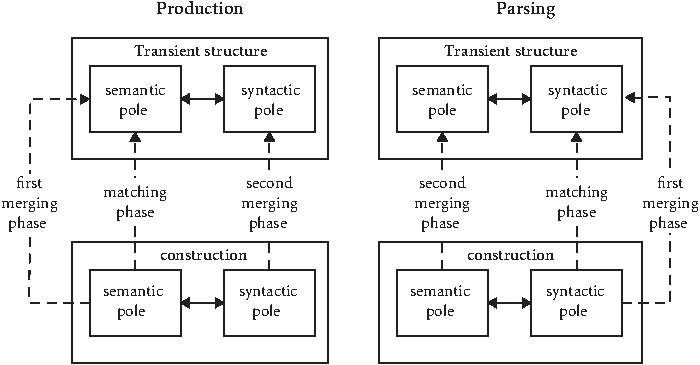
\includegraphics[width=.98\textwidth]{Figures/production-parsing-fcg.pdf}
\caption{\label{fig-matching-merging-trijp}Generation and parsing in FCG \citep[\page 99]{vanTrijp2013a}}
\end{figure}%

\subsubsection{Argument Structure Constructions}

Fluid Construction Grammar assumes a phrasal approach to argument structure, that is, it is assumed that lexical items enter
into phrasal configurations that contribute independent meaning \citep{vanTrijp2011a}. The FCG
approach is one version of implementing Goldberg's plugging approach to argument structure
constructions \citep{Goldberg95a}. Van Trijp suggests that every lexical item comes with a representation of
potential argument roles like Agent, Patient, Recipient, and Goal. Phrasal argument structure
constructions are combined with the respective lexical items and realize a subset of the argument
roles, that is they assign them to grammatical functions. Figure~\vref{fig-as-trijp} shows an
example: the verb \emph{sent} has the semantic roles Agent, Patient, Recipient, and Goal  (upper left
of the figure). Depending
on the argument structure construction that is chosen, a subset of these roles is selected for
realization.\footnote{
  It is interesting to note here that \citet[\page 141]{vanTrijp2011a} actually suggests a lexical
  account since every lexical item is connected to various phrasal constructions via coapplication
  links. So every such pair of a lexical item and a phrasal construction corresponds to a lexical
  item in Lexicalized Tree Adjoining Grammar (LTAG). See also \citew[\page 25]{MWArgSt} on
  Goldberg's assumption that every lexical item is associated with phrasal constructions.

Note that such coapplication links are needed since without them the approach cannot account for
cases in which two or more argument roles can only be realized together but not in isolation or in
any other combination with other listed roles.
}
%\todostefan{Are there Agent Goal verbs or Patient Recipient or Patient Goal verbs that allow for
%  patterns that are impossible for sent?}
The figures show the relation between sender, sent, and sendee and more the more abstract semantic
roles and the relation between these roles and grammatical functions for the sentences in (\mex{1}):
\eal
\ex He sent her the letter.
\ex He sent the letter.
\ex The letter was sent to her.
\zl
While in (\mex{0}a) the agent, the patient and the recipient are mapped to grammatical functions,
only the agent and the patient are mapped to grammatical functions in (\mex{0}b). The recipient is
left out. (\mex{0}c) shows an argument realization in which the sendee is realized as a \emph{to}
  phrase. According to van Trijp this semantic role is not a recipient but a goal. 


\begin{figure}
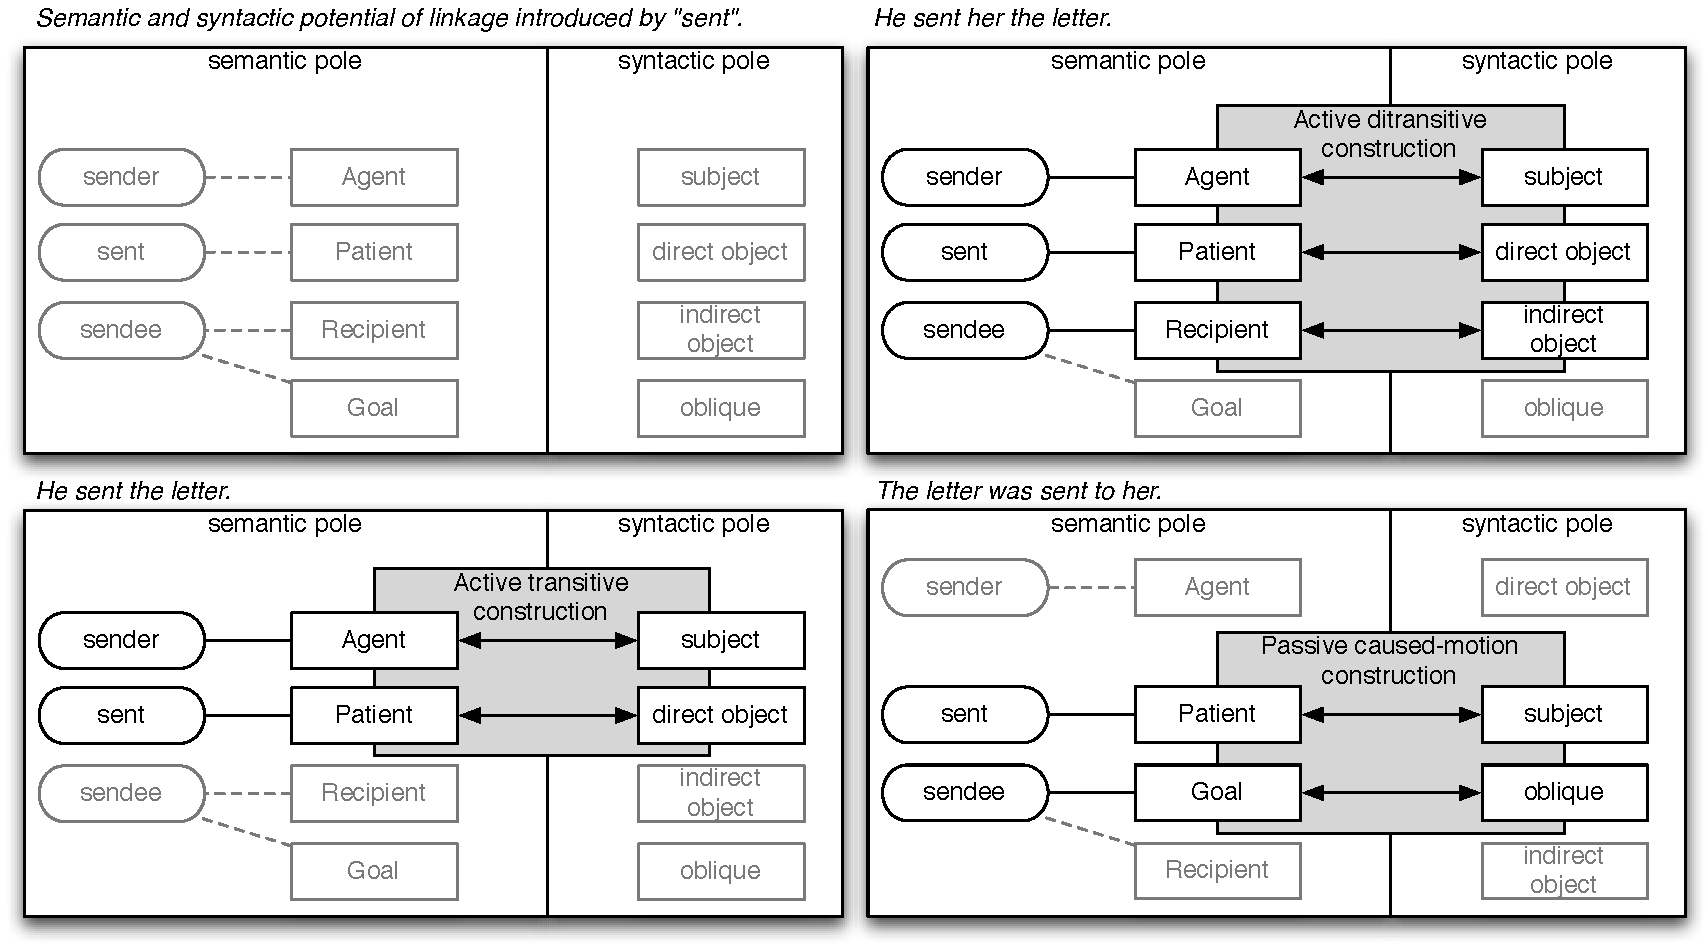
\includegraphics[width=\textwidth]{Figures/2011-van-Trijp.pdf}
\caption{\label{fig-as-trijp}Lexical items and phrasal constructions. Figure %taken 
from \citew[\page 122]{vanTrijp2011a}}
\end{figure}%

Note that under such an approach, it is necessary to have a passive variant of every active
construction. For languages that allow for the combination of passive and impersonal constructions,
one would be forced to assume a transitive-passive-impersonal construction. As was argued in
\citew[Section~2.6]{Mueller2006d} free datives (commodi/incommodi) in German can be added to almost
any construction. They interact with the dative passive and hence should be treated as
arguments. So, for the resultative construction one would need an active variant, a passive variant,
a variant with dative argument, a variant with dative argument and dative passive, and a middle variant.
While it is technically possible to list all these patterns and it is imaginable that we store all
this information in our brains, the question is whether such listings really reflect our linguistic
knowledge. If a new construction comes into existence, lets say an active sentence pattern with a
nominative and two datives in German, wouldn't we expect that this pattern can be used in the
passive? While proposals that establish relations between active and passive constructions would
predict this, alternative proposals that just list the attested possibilities do not.

%\addlines
The issue of how such generalizations should be captured was discussed in connection with the
organization of the lexicon in HPSG \citep{Flickinger87,Meurers2001a}. In the lexical world, one could simply categorize all verbs according to their
valence and say that \emph{loves} is a transitive verb and the passive variant \emph{loved} is an
intransitive verb. Similarly \emph{gives} would be categorized as a ditransitive verb and
\emph{given} as a two-place verb. Obviously this misses the point that \emph{loved} and \emph{given}
share something: they both are related to their active form in a systematic way. This kind of
generalization is captured by lexical rules that relate two lexical items. The respective
generalizations that are captured by lexical rules are called a horizontal generalizations as compared to vertical generalizations, which
describe relations between subtypes and supertypes in an inheritance hierarchy.

The issue is independent of the lexical organization of knowledge, it can be applied to phrasal
representations as well. Phrasal constructions can be organized in hierarchies (vertical), but the
relation between certain variants is not covered by this. The analog to the lexical rules in a
lexical approach are GPSG-like metarules in a phrasal approach. So what seems to be missing in FCG
is something that relates phrasal patterns, \eg allostructions (\citealp{Cappelle2006a}; \citealp[\page
  116]{Goldberg2014a}, see also footnote~\ref{fn-allostructions}).


\subsubsection{Fusion, matching and merging}

As was pointed out by \citet[\page 89--90]{Dowty89b-u}, checking for semantic compatibility is not sufficient
when deciding whether a verb may enter (or be fused with) a certain construction. The example is
the contrast between \emph{dine}, \emph{eat}, and \emph{devour}. While the thing that is eaten may
not be realized with \emph{dine}, its realization is optional with \emph{eat} and obligatory with
\emph{devour}. So the lexical items have to come with some information about
this. 

\Citet{vanTrijp2011a} and \citet{SvT2011a} make an interesting suggestion that could help
here: every verb comes with a list of potential roles and argument structure constructions can pick
subsets of these roles (see Figure~\ref{fig-as-trijp}). This is called \emph{matching}: introducing new argument roles is not allowed. 
This would make it possible to account for \emph{dine}: one could
say that there is something that is eaten, but that no Theme role is made available for linking to
the grammatical functions. This would be a misuse of thematic roles for syntactic purposes though
since \emph{dine} is semantically a two-place predicate. To account for the extension of argument roles as it is observed in the
Caused"=Motion Construction\is{construction!Caused"=Motion} \citep[Chapter~7]{Goldberg95a}, \citet{SvT2011a} suggest a process called \emph{merging}. Merging is seen
as a repair strategy: if an utterance involves an intransitive verb and some other material, the
utterance cannot be processed with matching alone. For example, when processing Goldberg's example
in (\mex{1}), \emph{he sneezed} could be parsed, but \emph{the foam} and \emph{off the cappuccino}
would be unintegrated (see Chapter~\ref{chap-phrasal} for an extended discussion of such constructions).
\ea
He sneezed the foam off the cappuccino.\footnote{
\citew[\page 42]{Goldberg2006a}.
}
\z
So, \citet[\page 319--320]{SvT2011a} suggest that only if regular constructions cannot apply, merging is
allowed. The problem with this is that human language is highly ambiguous and in the case
at hand this could result in situations in which there is a reading for an utterance, so that the
repair strategy would never kick in. Consider (\mex{1}):\footnote{
  I apologize for these examples \ldots. An English example that shows that there may be ambiguity
  between the depictive and the resultative construction is the following one that is due to
  \citet{Haider2016b}:
  \ea
  They cooked the chicken dry.
  \z
  I use the German example below since the resultative reading is strongly preferred over the
  depictive one.
}
\ea
\label{ex-schlag-den-mann-tot}
\gll Schlag den Mann tot!\\
     beat   the man  dead\\
\glt `Beat the man to death!' or `Beat the dead man!'
\z
(\mex{0}) has two readings: the resultative reading in which \emph{tot} `dead' expresses the result of the
beating and another reading in which \emph{tot} is a depictive predicate. The second reading is
dispreferred, since the activity of beating dead people is uncommon, but the structure is parallel to
other sentences with depictive predicates:
\ea
\gll Iss den Fisch roh!\\
     eat the fish raw\\
\z
The depictive reading can be forced by coordinating \emph{tot} with a predicate that is not a
plausible result predicate:
\ea
\gll Schlag ihn tot oder lebendig!\\
     beat   him dead or alive\\
\glt `Beat him when he is dead or while he is alive!'
\z
So, the problem is that (\ref{ex-schlag-den-mann-tot}) has a reading which does not require the invocation of the repair mechanism: \emph{schlug} `beat' is used with the transitive
construction and \emph{tot} is an adjunct (see \citealp{Winkler97a}). However, the more likely analysis of (\ref{ex-schlag-den-mann-tot}) is the one
with the resultative analysis, in which the valence frame is extended by an oblique element. So this
means that one has to allow the application of merging independent of other analyses that might be possible.
As \citet[\page 320]{SvT2011a} note, if merging is allowed to apply freely, utterances like
(\mex{1}a) will be allowed and of course (\mex{1}b) as well.
\eal
\ex[*]{
She sneezed her boyfriend.
}
\ex[*]{
She dined a steak.
}
\zl
In (\mex{0}) \emph{sneeze} and \emph{dined} are used in the transitive construction.

The way out of this dilemma is to establish information in lexical items that specifies in which
syntactic environments a verb can be used. This information can be weighted and for instance the
probability of \emph{dine} to be used transitively would be extremely low. Steels and van Trijp
would connect their lexical items to phrasal constructions via so-called coapplication links and the
strength of the respective link would be very low for \emph{dine} and the transitive construction and
reasonably high for \emph{sneeze} and the Caused"=Motion Construction\is{construction!Caused"=Motion}. This would explain the
phenomena (and in a usage"=based way), but it would be a lexical approach, as it is common in CG, HPSG,
SBCG, and DG.

\subsubsection{Long-distance dependencies}
\label{sec-fcg-nld}

%\addlines
\Citet{vanTrijp2014a} compares the \slasch-based approaches that are used in GPSG, HPSG, and SBCG
with the approach that he suggests within the framework of FCG. He claims that there are fundamental
differences between SBCG and FCG and assigns SBCG to the class of generative grammars, while
placing FCG in the class of cognitive"=functional approaches. He claims that his
cognitive"=functional approach is superior in terms of completeness, explanatory adequacy, and
theoretical parsimony (p.\,2). What \citet{vanTrijp2014a} suggests is basically an analysis that was
suggested by \citet{Reape2000a} in unpublished work (see \citew{Reape94a} for a published version of
an linearization"=based approach and \citew{Kathol2000a,Babel,Mueller99a,Mueller2002b} for
linearization"=based approaches that despite of being linearization"=based assume the \slasch approach for nonlocal dependencies). Van Trijp
develops a model of grammar that allows for discontinuous constituents and just treats the
serialization of the object in sentences like (\mex{1}) as an alternative linearization option.
\eal
\ex This book, I read.
\ex What did the boy hit?
\zl
Van Trijp's analysis involves several units that do not normally exist in phrase structure grammars,
but can be modeled via adjacency constraints or which represent relations between items which are part
of lexical representations in HPSG/SBCG anyway. An example is the subject-verb anchor that connects
the subject and the verb to represent the fact that these two items play an important functional
role. Figure~\vref{fig-what-did-the-boy-hit} shows the analysis of (\mex{1}).
\ea
What did the boy hit?
\z
\begin{figure}
\begin{forest}
for tree={l sep+=5mm}
%l sep+=10mm
[TRANSITVE-CLAUSE-UNIT, name=tcu
  [NP-UNIT-1, name=np1
    [PRO [what]] ]
  [AUX,tier=det, no edge, name=aux [did] ]
  [NP-UNIT-2, name=np2
    [DET, tier=det [the]]
    [N   [boy]] ]
  [VP-UNIT, name=vp
    [V [hit] ] ]
]
\draw (vp.south)--(aux.north);
\node (topic) [base left=of tcu]
    {
        TOPIC-UNIT
    };
\draw[dashed] (topic.south)--(np1.north);
\node (focus) [below=0mm of tcu.south west]
    {
        FOCUS-UNIT
    };
\draw[dashed] (focus.south)--(np1.north);
\draw[dashed] (focus.south)--(aux.north);
\node (sau) [base right= of tcu]
    {
        SV-ANCHOR-UNIT
    };
\draw[dashed] (sau.south)--(vp.north);
\draw[dashed] (sau.south)--(np2.north);
\end{forest}
\caption{\label{fig-what-did-the-boy-hit}The analysis of \emph{What did the boy hit?} according to
  \citet[\page 265]{vanTrijp2014a}}
\end{figure}%
As can be seen in the figure, van Trijp also refers to information structural\is{information structure} terms
like topic and focus. It should be noted here that the analysis of information structure has quite
some history in the framework of HPSG  \citep{EV96a, 
Kuhn95b,Kuhn96a, 
GuntherMaienborn1999,
Wilcock2001a,Wilcock2005a, 
deKuthy2002a,Paggio2005a-u, 
%\citet{Webelhuth2007a-u}, 
Bildhauer2008a,BC2010a}. The fact that information structure is not talked about in syntax
papers like \citew{Sag2012a} does not entail that information structure is ignored or should be
ignored in theories like HPSG and SBCG. So much for completeness. The same holds of course for
explanatory adequacy. This leaves us with theoretical parsimony, but before I comment on this, I
want to discuss van Trijp's analysis in a little bit more detail in order to show that many of his claims
are empirically problematic and that his theory therefore cannot be explanatory since empirical
correctness is a precondition for explanatory adequacy.

Van Trijp claims that sentences with nonlocal dependency constructions in English start with a
topic.\footnote{
\Citet[\page 256]{vanTrijp2014a} uses the following definitions for topic and focus: ``Topicality is defined in terms of aboutness: the topic of an utterance
is what the utterance is `about'. Focality is defined in terms of salience:
focus is used for highlighting the most important information given the
current communicative setting.''
} Bresnan's sentences in (\ref{bsp-fronted-focus}) and (\ref{bsp-fronted-topic}) were discussed on page~\pageref{bsp-fronted-focus}
\citep[\page 97]{Bresnan2001a} and are repeated below for convenience:
\ea
\label{bsp-fronted-focus-two}
Q: What did you name your cat?\\
A: Rosie I named her. (\emph{Rosie} = \textsc{focus})
\z
\ea
\label{bsp-fronted-topic-two}
Q: What did you name your pets?\\
A: My dog, I named Harold. My cat, I named Rosie. (\emph{my dog}, \emph{my cat} = \textsc{topic})
\z
These sentences show that the pre-subject position is not unambiguously a topic or a focus
position. So, a statement saying that the fronted element is a topic is empirically not correct. If this position is to be associated with an information structural function, this
association has to be a disjunction admitting both topics and focused constituents.

A further problematic aspect of van Trijp's analysis is that he assumes that the auxiliary \emph{do}
is an object marker (p.\,10, 22) or a non-subject marker (p.\,23). It is true that \emph{do} support is not necessary in subject questions like
(\mex{1}a), but only in (\mex{1}b), but this does not imply that all items that are followed by
\emph{do} are objects.
\eal
\ex Who saw the man?
\ex Who did John see?
\zl
First, \emph{do} can be used to emphasize the verb:
\ea
Who \emph{did} see the man?
\z
Second, all types of other grammatical functions can precede the verb:
\eal
\settowidth\jamwidth{(prepositional object)}
\ex Where did you see the man? \jambox{(adverbial)}
\ex How tall is the man? \jambox{(predicative)}
\ex What did John consider Peter? \jambox{(predicative)}
\ex What does this book cost? \jambox{(adverbial)}
\ex About what did you talk? \jambox{(prepositional object)}
\zl
And finally, even a subject can appear in front of \emph{do} if it is extracted from another clause:
\ea
\settowidth\jamwidth{(prepositional object)}
Who does he think saw this man? \jambox{(subject)}
\z
%
% Auch die linke Peripherie kann man ja einfach als kontinuierlich einordnen. Brauche Beleg für
% Extraposition aus pränominalem Adjunkt. Das würde mögliche Diskontinuität zeigen.
%
%% Van Trijp does not address the issue of island constraints. Extraction islands are areas that nobody
%% can leave, that is, extraction is excluded. For instance, it is impossible to extract from the
%% prenominal area in English and German (Ross' Left Branch Condition).
%\ea
%der die Frau liebende Mann, die ... erfunden hat
%%  and it is also impossible to
%% extract out of a relative clause:
%% % Er könnte sagen, dass Relativsätze immer kontinuierlich sein müssen.
%% \ea
%% This man$_i$, I saw a women [who likes \_$_i$ ].
%% \z
%% \slasch"=based models assume that relative clauses involve internal nonlocal dependencies, but no
%% \slasch dependency leaves the relative clause. This is ensured by the schemata that combine the
%% relative pronoun and the remaining clause.

There is a further empirical problem: approaches that assume that a filler is related to its origin
can explain scope ambiguities that only arise when an element is extracted. Compare for instance the
sentence in (\mex{1}a) with the sentences in (\mex{1}b, c): although the order of \emph{oft} `often' and
\emph{nicht} `not' in (\mex{1}a) and (\mex{1}c) is the same, (\mex{1}a) is ambiguous but (\mex{1}c) is
not.
\eal
\ex 
\gll Oft liest er das Buch nicht.\\
     often reads he the book not\\
\glt `It is often that he does not read the book.' or `It is not the case that he reads the book
often.'
\ex
\gll dass er das Buch nicht oft liest\\
     that he the book not often reads\\
\glt `that it is not the case that he reads the book often'
\ex
\gll dass er das Buch oft nicht liest\\
     that he the book often not reads\\
\glt `that it is often that he does not read the book'
\zl
(\mex{0}a) has the two readings that correspond to (\mex{0}b) and (\mex{0}c). A purely
linearization"=based approach probably has difficulties to explain this. A \slasch"=based approach
can assume that (\mex{0}a) has a gap (or some similar means for the introduction of nonlocal
dependencies) at the position of \emph{oft} in (\mex{0}b) or (\mex{0}c). The gap information is
taken into account in the semantic composition at the site of the gap. This automatically accounts
for the observed readings.

Another empirical problem that has to be solved is the existence of extraction path
marking\is{extraction path marking}
languages. \citet*{BMS2001a} list a number of languages in which elements vary depending on the
existence or absence of a gap in a constituent they attach to. For instance, Irish has
complementizers that have one form if the clause they attach to has an element extracted and another
form if it does not. \slasch-based proposals can account for this in a straight-forward way: the
fact that a constituent is missing in a phrase is represented in the \slashv of the trace and this
information is percolated up the tree. So even complex structures contain the information that there
is a constituent missing inside them. Complementizers that are combined with sentences therefore can
select sentences with \slashvs that correspond to the form of the complementizer.
Van Trijp's answer to this challenge is that all languages are different
\citep[\page 263]{vanTrijp2014a} and that the evidence from one language does not necessarily mean that the analysis for that language is
also appropriate for another language. While I agree with this view in principle (see
Section~\ref{sec-syntactic-universals}), I do think that extraction is a rather fundamental property
of languages and that nonlocal dependencies should be analyzed in parallel for those languages that
have it.


\subsection{Coordination}
\label{sec-coordination}

One of the success stories of non-transformational grammar is the \slasch-based analysis of nonlocal dependencies
by \citet{Gazdar81}. This analysis made it possible for the first time to explain Ross's Across the Board
Extraction\is{Across the Board Extraction} \citep{Ross67}. The examples were already discussed on
page~\pageref{ex-atb-gazdar} and are repeated here for convenience:
\eal\settowidth\jamwidth{(= S/NP \& S/NP)}
\label{ex-atb-gazdar-two}
\ex[]{ The kennel     which Mary made and Fido sleeps in has been stolen.	 \jambox{(= S/NP \& S/NP)}
}
\ex[]{ The kennel in which Mary keeps drugs and Fido sleeps has been stolen.	\jambox{(= S/PP \& S/PP)}
}
\ex[*]{The kennel (in) which Mary made and Fido sleeps has been stolen.     \jambox{(= S/NP \& S/PP)}
}
\zl
The generalization is that two (or more) constituents can be coordinated if they have identical
syntactic categories and identical \slashvs. This explains why \emph{which} and \emph{in which} in
(\mex{0}a,b) can fill two positions in the respective clauses. Now, theories that do not use a
\slashf for the percolation of information about missing elements have to find different ways to
make sure that all argument slots are filled and that the correct correspondence between extracted
elements and the respective argument role is established. Note that this is not straightforward in
models like the one suggested by van Trijp, since he has to allow the preposition \emph{in} to be
combined with some material to the left of it that is simultaneously also the object of
\emph{made}. Usually an NP cannot simply be used by two different heads as their argument. As an
example consider (\mex{1}a):
\eal
\ex[*]{
John said about the cheese that I like.
}
\ex[]{
John said about the cheese that I like it.
}
\zl
If it would be possible to use material several times, a structure for (\mex{0}a) would be possible
in which \emph{the cheese} is the object of the preposition \emph{about} and of the verb
\emph{like}. This sentence, however, is totally out: the pronoun \emph{it} has to be used to fill
the object slot.


\subsection{Discontinuous constituents and performance models}

Van Trijp points out that SBCG does not have a performance model and contrasts this with FCG. On
page~252 he states:
\begin{quote}
So parsing starts by segmenting the utterance
into discrete forms, which are then categorized into words by morphological
and lexical constructions, and which can then be grouped together as
phrases (see Steels, 2011b, for a detailed account of lexico-phrasal
processing in FCG). So the parser will find similar constituents for all
four utterances, as shown in examples (21--24). Since auxiliary-\emph{do} in
example (24) falls outside the immediate domain of the VP, it is not yet
recognized as a member of the VP.

All of these phrases are disconnected, which means that the grammar
still has to identify the relations between the phrases. \citep[\page 252]{vanTrijp2014a}
\end{quote}
In his (21)--(24), van Trijp provides several tree fragments that contain NPs for subject and object and states that
these have to be combined in order to analyze the sentences he discusses. This is empirically
inadequate: if FCG does not make the competence/performance distinction, then the way utterances are
analyzed should reflect the way humans process language (and this is what is usually claimed about FCG). However, all we know about human language
processing points towards an incremental processing, that is, we process information as soon as it
is available. We start to process the first word taking into account all of the relevant aspects
(phonology, stress, part of speech, semantics, information structure) and come up with an hypothesis
about how the utterance could proceed. As soon as we have two
words processed (in fact even earlier: integration already happens during the processing of words) we integrate the second word
into what we know already and continue to follow our hypothesis, or revise it, or simply fail. See
Section~\ref{Abschnitt-Inkrementelle-Verarbeitung} for details on processing and the discussion of
experiments that show that processing is incremental. So, we have to say that van Trijp's analysis
fails on empirical grounds: his modeling of performance aspects is not adequate.

The parsing scheme that van Trijp describes is pretty much similar to those of computational HPSG parsers, but
these usually come without any claims about human performance. Modeling human performance is rather complex
since a lot of factors play a role. It is therefore reasonable to separate competence and
performance and continue to work the way it is done in HPSG and FCG. This does not mean that
performance aspects should not be modeled, in fact psycholinguistic models using HPSG have been
developed in the past \citep{Konieczny96a-u}, but developing both a grammar with large coverage and
the performance model that combines with it demands a lot of resources.

\subsection{Discontinuity vs.\ Subject-Head and Head-Filler Schema}
\label{sec-discontinuous-constituents-fcg}

I now turn to parsimony: van Trijp uses a subject-verb anchor construction that combines the subject
and the main verb. Because of examples like (\mex{1}) it must be possible to have discontinuous subject-verb constructions:\footnote{
  Unless modals and tense auxiliaries are treated as main verbs (which they should not in English), constructions with
  modals seem to be another case where the subject and the main verb are not adjacent:
  \eal
  \ex Peter will read the book.
  \ex Peter has read the book.
  \zllast
} 
\ea
Peter often reads books.
\z
But if such constructions can be discontinuous one has to make sure that (\mex{1}b) cannot be an
instantiation of the subject-verb construction:
\eal
\ex[]{
The boy I think left.
}
\ex[*]{
I the boy think left.
}
\zl
Here it is required to have some adjacency between the subject and the verb it belongs to, modulo
some intervening adverbials. This is modelled quite nicely in phrase structure grammars that have a
VP node. Whatever the internal structure of such a VP node may be, it has to be adjacent to the
subject in sentences like  (\mex{-1}) and (\mex{0}a) above. The dislocated element has to be adjacent to the complex
consisting of subject and VP. This is what the Filler-Head Schema does in HPSG and SBCG. Van Trijp
criticizes SBCG for having to stipulate such a schema, but I cannot see how his grammar can be
complete without a statement that ensures the right order of elements in sentences with fronted
elements.

Van Trijp stated that FCG differs from what he calls generative approaches in that it does not want
to characterize only the well-formed utterances of a language. According to him, the parsing direction
 is much more liberal in accepting input than other theories. So it could well be that he
is happy to find a structure for (\mex{0}b). Note though that this is incompatible with other claims
made by van Trijp: he argued that FCG is superior to other theories in that it comes with a performance
model (or rather in not separating competence from performance at all). But then (\mex{0}b) should be
rejected both on competence and performance grounds. It is just unacceptable and speakers reject it
for whatever reasons. Any sufficiently worked out theory of language has to account for this.


\subsection{Restricting discontinuity}
\label{sec-restricting-discont}

There is a further problem related to discontinuity. If one does not restrict continuity, then
constituent orders like (\mex{1}b) are admitted by the grammar:
\eal
\ex[]{
\gll Deshalb klärt, dass Peter kommt, ob Klaus spielt.\\
     therefore resolves that Peter comes whether Klaus plays\\
\glt `Therefore that Peter comes resolves whether Klaus will play.'
}
\ex[*]{
\gll Deshalb klärt dass ob Peter Klaus kommt spielt.\\
     therefore resolves that whether Peter Klaus comes plays\\
}
\zl
The interesting thing about the word salad in (\mex{0}b) is that the constituent order within the
\emph{dass} clause and within the \emph{ob} clause is correct. That is, the complementizer precedes
the subject, which in turn precedes the verb. The problem is that the constituents of the two
clauses are mixed. 
%% Note that the clausal arguments can appear in both orders:
%% \ea
%% \gll Deshalb klärt, ob Klaus spielt, dass Peter kommt.\\
%%      therefore resolves whether Klaus comes that Peter comes\\
%% \z
%% Therefore 

In a model that permits discontinuous constituents, one cannot require that all parts of an argument have
to be arranged after all parts that belong to another argument since discontinuity is used to
account for nonlocal dependencies. So, it must be possible to have \emph{Klaus} before other
arguments (or parts of other arguments) since \emph{Klaus} can be extracted. An example of mixing
parts of phrases is given in (\mex{1}):
\ea
\gll Dieses Buch hat der Mann mir versprochen, seiner Frau zu geben, der gestern hier aufgetreten ist.\\
     this   book has the man  me  promised     his    wife to give   who yesterday here performed is\\
\glt `The man who performed here yesterday promised me to give this book to his wife.'
\z 
%\addlines[2]
We see that material that refers to \emph{der Mann} `the man', namely the relative clause \emph{der gestern
  hier aufgetreten ist} `who performed here yesterday', appears to the right. And the object of
\emph{geben} `to give', which would normally
be part of the phrase \emph{dieses Buch seiner Frau zu geben} `this book his wife to give' appears to the left. So, in general it
is possible to mix parts of phrases, but this is possible in a very restricted way only. Some
dependencies extend all the way to the left of certain units (fronting) and others all the way to the right
(extraposition). Extraposition is clause-bound, while extraction is not. In approaches like GPSG,
HPSG and SBCG, the facts are covered by assuming that constituents for a complete clause are
continuous apart from constituents that are fronted or extraposed. The fronted and extraposed
constituents are represented in \slasch and \extra (\citealp{Keller95b};
\citealp[Section~13.2]{Mueller99a}; \citealp{Crysmann2013a}), respectively, rather than in valence features,
so that it is possible to require of constituents that have all their valents saturated to be
continuous \citep[\page 294]{Mueller99g}.

Summing up the discussion of parsimony, it has to be said that van Trijp has to provide the details
on how continuity is ensured. The formalization of this is not trivial and only after this is done
can FCG be compared with the \slasch"=based approach.

In addition to all the points discussed so far, there is a logical flaw in van Trijp's argumentation.
He states that:
\begin{quote}
whereas the filler-gap analysis cannot explain \textsc{why} \emph{do}-support does not occur
  in \emph{wh}-questions where the subject is assigned questioning focus, this follows naturally
from the interaction of different linguistic perspectives in this paper's
approach. \citep[\page 263]{vanTrijp2014a}
\end{quote}
The issue here is whether a filler-gap analysis or an analysis with discontinuous
constituents is suited better for explaining the data. A correct argumentation against the filler-gap analysis would require a proof that information structural or other functional constraints
cannot be combined with this analysis. This proof was not provided and in fact I think it cannot be
provided since there are approaches that integrate information structure. Simply pointing out that a
theory is incomplete does not falsify a theory. This point was already made in my review of
\citew{Boas2003a} and in a reply to \citet{Boas2014a}. See \citew[655--656]{Mueller2005a},
\citew[Chapter~20]{MuellerLehrbuch1}, and \citew[Footnote~15]{MWArgStReply}.

The conclusion about the FCG analysis of nonlocal dependencies is that there are some empirical
flaws that can be easily fixed or assumptions that can simply be dropped (role of \emph{do} as object marker, claim that
the initial position in English fronting construction is the topic), some empirical shortcomings
(coordination, admittance of illformed utterances with discontinuous constituents), some empirical
problems when the analysis is extended to other languages (scope of adjuncts in German), and the
parsimony of the analyses is not really comparable since the restrictions on continuity are not
really worked out (or at least not published). If the formalization of restrictions on continuity in FCG turns out to be even
half as complex as the formalization that is necessary for accounts of nonlocal dependencies
(extraction and extraposition) in linearization"=based HPSG that \citet{Reape2000a}
suggested,\footnote{
  See \citew{KP95a} for a linearization"=based account of extraposition. This account is
  implemented in the Babel System \citep{Babel}. See \citep{Mueller99g} on restricting
  discontinuity. Linearization"=based approaches were argued to not be able to account for
  apparent multiple frontings in German \citep{Mueller2005d,MuellerGS} and hence
  linearization"=based approaches were replaced by more traditional variants that allow for
  continuous constituents only.
} the \slasch"=based analysis would be favorable.

In any case, I do not see how nonlocal dependencies could be used to drive a wedge between SBCG and
FCG. If there are functional considerations that have to be taken into account, they should be
modeled in both frameworks. In general, FCG should be more restrictive than SBCG since FCG claims to
integrate a performance model, so both competence and performance constraints should be operative. I
will come back to the competence/""performance distinction in the following section, which is a more
general comparison of SBCG and FCG.

\subsubsection{Comparison to Sign-Based Construction Grammar/HPSG}


According\indexhpsgstart\indexsbcgstart to \citet{vanTrijp2013a}, there are the differences shown in Table~\vref{table-differences-SBCG-FCG}.
%% \begin{itemize}
%% \item
%% \label{fcg-sbcg-generative} SBCG embraces a generative conception of linguistic theory, whereas FCG adopts a
%%   cognitive-functional approach (p.\,89)
%% \item
%% \end{itemize}
%
% moved to top
These differences will be discussed in the following subsections.
\begin{table}
\caption{\label{table-differences-SBCG-FCG}Differences between SBCG and FCG according to \citet[\page 112]{vanTrijp2013a}}
\begin{tabular}{@{}lll@{}}\hline\hline
Scientific model    & Theoretical physics           & Evolutionary theory\\
                    & (abstract calculus)           &  (complex adaptive system)\\
Linguistic approach & Generative                    & Cognitive-functional\\
                    & (competence model)            & (parsing and production)\\
Formalization       & Mathematical                  & Computational\\ 
                    & (amenable for implementation) & (implemented)\\
Constructions       & Static type constraints       & Dynamic mappings\\
Constructicon       & Signature and grammar         & Open-ended inventory\\
Processing          & Assumption of processing-     & Bidirectional processing\\
                    & independence                  & model\\\hline\hline
\end{tabular}
\end{table}%

\subsubsubsection{Competence/performance distinction}
\label{sec-performance-cxg}

As\is{competence|(}\is{performance|(} for the linguistic approach, the use of the term \emph{generative} is
confusing. What van Trijp means -- and also explains in the paper -- is the idea that one should
separate competence and performance. We will deal with both the generative-enumerative
vs.\ constraint-based view and with the competence/performance distinction in more detail in the
Chapters~\ref{Abschnitt-Generativ-Modelltheoretisch} and~\ref{Abschnitt-Diskussion-Performanz},
respectively. Concerning the cognitive-functional approach, van Trijp writes:
\begin{quote}
The goal of a cognitive-functional grammar, on the other hand, is to explain
how speakers express their conceptualizations of the world through language
(= \emph{production}) and how listeners analyze utterances into meanings (= \emph{parsing}).
Cognitive-functional grammars therefore implement both a competence and a
processing model. \citep[\page 90]{vanTrijp2013a}
\end{quote}
It is true that HPSG and SBCG make a competence/performance distinction \citep{SW2011a}. HPSG
theories are theories about the structure of utterances that are motivated by distributional
evidence. These theories do not contain any hypothesis regarding brain activation, planning of
utterances, processing of utterances (garden path effects) and similar things. In fact, none of the
theories that are discussed in this book contains an explicit theory that explains all these
things. I think that it is perfectly legitimate to work in this way: it is legitimate to study the
structure of words without studying their semantics and pragmatics, it is legitimate to study
phonology without caring about syntax, it is legitimate to deal with specific semantic problems
without caring about phonology and so on, provided there are ways to integrate the results of such
research into a bigger picture. In comparison, it is wrong to develop models like those developed in current
versions of Minimalism\indexmp (called Biolinguistics\is{Biolinguistics}), where it is assumed that utterances are derived in
phases\is{phase} (NPs, CPs, depending on the variant of the theory) and then shipped to the interfaces\is{interface} (spell
out and semantic interpretation). This is not what humans do (see
Chapter~\ref{Abschnitt-Diskussion-Performanz}).\footnote{
Attempts to integrate current Minimalist theories with psycholinguistic findings \citep{Phillips2003a} are
incompatible with core principles of Minimalism like the \emph{No Tampering Condition}\is{No
  Tampering Condition (NTC)} of \citet{Chomsky2008a}.
}
But if we are neutral with respect towards such
issues, we are fine. In fact, there is psycholinguistic work that couples HPSG grammars to
performance models \citep{Konieczny96a-u} and similar work exists for TAG \citep{SJ93a,DK2008a-u}. 

%\addlines[-1]
Finally, there is also work in Construction Grammar that abstracts away from performance
considerations. For instance, Adele Goldberg's book from \citeyear{Goldberg95a} does
not contain a worked out theory of performance facts. It contains boxes in which grammatical
functions are related to semantic roles. So this basically is a competence theory as well. Of course
there are statements about how this is connected to psycholinguistic findings, but this is also true
for theories like HPSG, SBCG and Simpler Syntax \citep[\page 600]{Jackendoff2011a} that explicitly make the competence/performance distinction.\is{competence|)}\is{performance|)}

\subsubsubsection{Mathematical formalization vs.\ implementation}

The difference between mathematical and computational formalization is a rather strange distinction to make. I
think that a formal and precise description is a prerequisite for implementation (see the discussion
in Section~\ref{sec-formalization-gb} and Section~\ref{sec-formalization-minimalism}). Apart from this, a computer implementation of SBCG is
trivial, given the systems that we have for processing HPSG grammars. In order to show this, I want
to address one issue that van Trijp discusses. He claims that SBCG cannot be directly
implemented. On issues of complexity of constraint solving systems he quotes \citep[Section~4.2.2]{LM2006a}:
\begin{quote}
Actual implementations of HPSG typically handle the problem by guiding the linguistic processor
using a (rule-based) phrase structure backbone, but the disadvantage of this approach is that the ``organization and formulation of the grammar is different from
that of the linguistic theory'' \citep[Section~4.2.2]{LM2006a}. \citep[\page 108]{vanTrijp2013a}
\end{quote}
He concludes:
\begin{quote}
Applying all these observations to the operationalization of SBCG, we can
conclude that an SBCG grammar is certainly amenable for computational implementation because of its formal explicitness. There are at least two computational
platforms available, mostly used for implementing HPSG-based grammars, whose
basic tenets are compatible with the foundations of SBCG: LKB \citep{Copestake2002a}
and TRALE\is{TRALE} (Richter 2006). However, none of these platforms supports a `direct'
implementation of an SBCG grammar as a general constraint system, so SBCG's
performance-independence hypothesis remains conjecture until proven otherwise.
\end{quote}
%\addlines
There are two issues that should be kept apart here: efficiency and faithfulness to the
theory. First, as Levine and Meurers point out, there were many constraint solving systems at the
beginning of the 90's. So there are computer systems that can and have been used to implement
and process HPSG grammars. This is very valuable since they can be used for direct verification of
specific theoretical proposals. As was discussed by Levine and Meurers, trying to solve constraints
without any guidance is not the most efficient way to deal with the parsing/generation
problem. Therefore, additional control-structure was added. This control structure is used for
instance in a parser to determine the syntactic structure of a phrase and other constraints will
apply as soon as there is sufficient information available for them to apply. For instance, the
assignment of structural case happens once the arguments of a head are realized. Now, is it bad to
have a phrase structure backbone? One can write down phrase structure grammars that use phrase
structure rules that have nothing to do with what HPSG grammars usually do. The systems TRALE \citep*{MPR2002a-u,Penn2004a-u} and
LKB will process them. But one is not forced to do this. For instance, the grammars that I developed
for the CoreGram project \citep{MuellerCoreGramBrief,MuellerCoreGram} are very close to the linguistic theory. To see that this is really the
case, let us look at the Head-Argument Schema. The Head-Argument Schema is basically the type
\type{head-argument-phrase} with certain type constraints that are partly inherited from its
supertypes. The type with all the constraints was given on page~\pageref{head-arg-schema-hfp} and is
repeated here as (\mex{1}):
\eas
\label{head-arg-schema-hfp-zwei}
(syntactic) constraints on \type{head-argument-phrase}:\\
\onems[head-argument-phrase~]{
synsem$|$loc$|$cat  \ms{ head   & \ibox{1} \\
                          subcat & \ibox{2}
                        }\\
head-dtr$|$synsem$|$loc$|$cat \ms{ head   & \ibox{1} \\
                                   subcat & \ibox{2} $\oplus$ \sliste{ \ibox{3} }
                                 } \\
non-head-dtrs   \sliste{ [ synsem \ibox{3} ] }
}
\zs
%\addlines
This can be translated into phrase structure grammar rules in a straight-forward way:
\eal
\ex \onems[head-argument-phrase~]{
synsem$|$loc$|$cat  \ms{ head   & \ibox{1} \\
                          subcat & \ibox{2}
                        }\\
head-dtr \ibox{4} $|$synsem$|$loc$|$cat \ms{ head   & \ibox{1} \\
                                   subcat & \ibox{2} $\oplus$ \sliste{ \ibox{3} }
                                 } \\
non-head-dtrs   \sliste{ \ibox{5} [ synsem \ibox{3} ] }
} $\to$ \ibox{4}, \ibox{5}
\ex \onems[head-argument-phrase~]{
synsem$|$loc$|$cat  \ms{ head   & \ibox{1} \\
                          subcat & \ibox{2}
                        }\\
head-dtr \ibox{4} $|$synsem$|$loc$|$cat \ms{ head   & \ibox{1} \\
                                   subcat & \ibox{2} $\oplus$ \sliste{ \ibox{3} }
                                 } \\
non-head-dtrs   \sliste{ \ibox{5} [ synsem \ibox{3} ] }
} $\to$ \ibox{5}, \ibox{4}
\zl
The left hand side of the rule is the mother node of the tree, that is, the sign that is licensed by
the schema provided that the daughters are present. The right hand side in (\mex{0}a) consists of
the head daughter \iboxt{4} followed by the non-head daughter \ibox{5}. We have the opposite order
in (\mex{0}b), that is, the head daughter follows the non-head daughter. The two orders correspond
to the two orders that are permitted by LP-rules: the head precedes its argument if it is marked
\textsc{initial}+ and it follows it if it is marked \textsc{initial}$-$.

The following code shows how (\mex{0}b) is implemented in TRALE:
\begin{verbatim}
arg_h rule (head_argument_phrase,
          synsem:loc:cat:head:initial:minus,
          head_dtr:HeadDtr,
          non_head_dtrs:[NonHeadDtr]
         )
  ===>
cat> NonHeadDtr,
cat> HeadDtr.
\end{verbatim}
A rule starts with an identifier that is needed for technical reasons like displaying intermediate
structures in the parsing process in debugging tools. A description of the mother node follows and
after the arrow we find a list of daughters, each introduced by the operator \verb+cat>+.\footnote{
  Other operators are possible in TRALE. For instance, \texttt{sem\_head} can be used to guide the
  generator. This is control information that has nothing to do with linguistic theory and not
  necessarily with the way humans process natural language. There is also a \texttt{cats} operator,
  which precedes lists of daughters. This can be used to implement phrase structures with more than
  one non-head daughter.%
}
Structure sharing is indicated by values with capital letters. The above TRALE rule is a
computer"=readable variant of (\mex{0}b) additionally including the explicit specification of the value of {\initial}.  

Now, the translation of a parallel schema using a \textsc{mother} feature like (\mex{1}a) into a phrase structure rule is almost as simple:
\eal
\ex \onems[head-argument-cx~]{
mother$|$synsem$|$loc$|$cat  \ms{ head   & \ibox{1} \\
                                  subcat & \ibox{2}
                        }\\
head-dtr$|$synsem$|$loc$|$cat \ms{ head   & \ibox{1} \\
                                   subcat & \ibox{2} $\oplus$ \sliste{ \ibox{3} }
                                 } \\
non-head-dtrs   \sliste{ [ synsem \ibox{3} ] }
}

\ex 
\ibox{6} $\to$ \ibox{4}, \ibox{5} where \onems[head-argument-cx~]{
mother \ibox{6} $|$synsem$|$loc$|$cat  \ms{ head   & \ibox{1} \\
                          subcat & \ibox{2}
                        }\\
head-dtr \ibox{4} $|$synsem$|$loc$|$cat \ms{ head   & \ibox{1} \\
                                             subcat & \ibox{2} $\oplus$ \sliste{ \ibox{3} }
                                 } \\
non-head-dtrs   \sliste{ \ibox{5} [ synsem \ibox{3} ] }
}
\zl
(\mex{0}b) is only one of the two phrase structure rules that correspond to (\mex{0}a), but since
the other one only differs from (\mex{0}b) in the ordering of \iboxt{4} and \iboxt{5}, it is not
given here.

For grammars in which the order of the elements corresponds to the observable order of the
daughters in a \textsc{dtrs} list, the connection to phrase structure rules is even simpler:
\ea 
\ibox{1} $\to$ \ibox{2} where \ms[construction~]{
mother & \ibox{1} \\
dtrs   & \ibox{2}
}
\z
%\addlines[2]
The value of \textsc{dtrs} is a list and hence \iboxt{2} stands for the list of daughters on the right
hand side of the phrase structure rule as well. The type \type{construction} is a supertype of all
constructions and hence (\mex{0}) can be used to analyze all phrases that are licensed by the
grammar. In fact, (\mex{0}) is one way to put the meta constraint in (\ref{meta-construction-statemnet}).

So, this shows that the version of SBCG that has been developed by \citet{Sag2012a} has a
straightforward implementation in TRALE.\footnote{%
A toy fragment of English using a \textsc{mother} feature and phrase structure rules with specifications
of the kind given above can be downloaded at \url{https://hpsg.hu-berlin.de/Fragments/SBCG-TRALE/}.%
}
The question remains whether ``SBCG's performance"=independence hypothesis remains conjecture until proven otherwise'' as van Trijp sees
it. The answer is: it is not a conjecture since any of the old constraint-solving systems of the
nineties could be used to process SBCG. The question of whether this is efficient is an engineering
problem that is entirely irrelevant for theoretical linguistics. Theoretical linguistics is
concerned with human languages and how they are processed by humans. So whether some processing system
that does not make any claims about human language processing is efficient or not is absolutely
irrelevant. Phrase structure-based backbones are therefore irrelevant as well, provided they refer
to the grammar as described in theoretical work.  

Now, this begs the question whether there is a contradiction in my claims. On
page~\pageref{page-sbcg-formalization} I pointed out that SBCG is lacking a formalization in
Richter's framework \citep{Richter2004a-u}. Richter and also \citet{LM2006a} pointed out that there are problems with
certain theoretically possible expressions and it is these expressions that mathematical linguists care
about. So the goal is to be sure that any HPSG grammar has a meaning and that it is clear what it
is. Therefore, this goal is much more foundational than writing a single grammar for a particular fragment
of a language. There is no such foundational work for FCG since FCG is a specific toolkit that has been used
to implement a set of grammars.

\subsubsubsection{Static constraints vs.\ dynamic mappings and signature $+$ grammar vs.\ open-endedness}

%\addlines
On very interesting feature of Fluid Construction Grammar is its fluidity, that is there are certain
constraints that can be adapted if there is pressure, the inventory of the theory is open-ended, so
categories and features can be added if need be.

Again, this is not a fundamental difference between HPSG/SBCG and FCG. An HPSG grammar fragment of a
specific language is a declarative representation of linguistic knowledge and as such it of course
just represents a certain fragment and does not contain any information how this set of constraints
evolved or how it is acquired by speakers. For this we need specific theories about language
evolution/"language change/"language acquisition. This is parallel to what was said about the
competence/performance distinction, in order to account for language evolution we would have to have
several HPSG grammars and say something about how one developed from the other. This will involve
weighted constraints, it will involve recategorization of linguistic items and lots more.\footnote{
  There are systems that use weighted constraints. We had a simple version of this in the
  German HPSG grammar that was developed in \verbmobil project \citep{MK2000a} already. Further
  theoretical approaches to integrate weighted constraints are \citew{Brew95a} and more recently
  \citew{Guzman-Naranjo2015a}. Usually such weighted constraints are not part of theoretical papers,
  but there are exceptions as for instance the paper by Briscoe and Copestake about lexical rules \citep{BC99a}.
} So basically HPSG has to be extended, has to be paired with a model about
language evolution in the very same way as FCG is.



\subsubsubsection{Theoretical physics vs.\ Darwinian evolutionary theory}

Van Trijp compares SBCG and FCG and claims that SBCG follows the model of theoretical physics --
like Chomsky does --, while FCG adopts a Darwinian model of science -- like Croft does --, the difference
being that SBCG makes certain assumptions that are true of all languages, while FCG does not make
any a priori assumptions. The fundamental assumptions made in both theories are that the
objects that we model are best described by feature value pairs (a triviality). FCG assumes that
there is always a syntactic and a semantic pole (fundamental assumption in the system) and
researchers working in HPSG/SBCG assume that if languages have certain phenomena, they will be
analyzed in similar ways. For instance, if a language has nonlocal dependencies, these will be
analyzed via the \slasch mechanism. However, this does not entail that one believes that grammars of
all languages have a \slashf. And in fact, there may even be languages that do not have valence
features \citep{KM2010a-u}, which may be a problem for FCG since it relies on the SYN-pole for the
matching phase. So as far as SBCG is concerned, there is considerable freedom to choose features
that are relevant in an analysis, and of course additional features and types can be assumed in case
a language is found that provides evidence for this. The only example of a constraint provided by van Trijp that is possibly too strong
 is the locality constraint imposed by the \textsc{mother}
feature. The idea about this feature is that everything that is of relevance in a more nonlocal
context has to be passed up explicitly. This is done for nonlocal dependencies (via \slasch) and for instance also
for information concerning the form of a preposition inside of a PP (via \textsc{pform} or more
recently via \form). Certain verbs require prepositional objects and restrict
the form of the preposition. For instance, \emph{wait} has to make sure that its prepositional
object has the preposition \emph{for} in it. Since this information is usually available only at the
preposition, it has to be passed up to the PP level in order to be directly selectable by the
governing verb. 
\ea
I am waiting for my man.
\z 
%\addlines[2]
So, assuming strict locality of selection requires that all phenomena that cannot be treated locally
have to be analyzed by passing information up.
%% \footnote{
%%   It should also be noted that \citet[\page 111]{vanTrijp2013a} draws hasty conclusions when he
%%   writes: \emph{the locality of SBCG constructions, which entails that all languages can best be
%% described as constraints on local trees.} Depending on the definition of tree 
%% }
Assuming strict locality is a design decision that does not have any empirical consequences, as far
as it does not rule out any language or construction in principle. It just requires that information
has to be passed up that needs to be accessed at higher nodes. As I have shown in Section~\ref{sec-SbCxG},
the locality constraint is easily circumvented even within SBCG and it makes the analysis of idioms
unnecessarily complicated and unintuitive, so I suggest dropping the \textsc{mother} feature. But even if \textsc{mother} is kept, it is not justified to draw a
distinction between SBCG and FCG along the lines suggested by van Trijp. 

Independent of the \textsc{mother} issue, the work done in the CoreGram project
\citep{MuellerCoreGramBrief,MuellerCoreGram} shows that one can derive generalizations in a
bottom-up fashion rather than imposing constraints on grammars in a top-down way. The latter paper
discusses Croft's methodological considerations and shows how methodological pitfalls are
circumvented in the project. HPSG/SBCG research differs from work in Chomskyan frameworks in not
trying to show that all languages are like English or Romance or German or whatever, rather
languages are treated on their own as it is common in the Construction Grammar community. This does
not imply that there is no interest in generalizations and universals or near universals or tendencies, but again
the style of working and the rhetoric in HPSG/SBCG is usually different from the ones in Mainstream
Generative Grammar. Therefore, I think that the purported difference
between SBCG and FCG does not exist.

\subsubsubsection{Permissiveness of the theories}

Van Trijp claims that HPSG/SBCG is a ``generative grammar'' since its aim is to account for and admit only
grammatical sentences. FCG on the other hand is more permissive and tries to get the most out of the
input even if it is fragmentary or ungrammatical (see also \citealp[\page 166]{Steels2013a}). While it is an engineering decision to be able to parse ungrammatical input --  and 
 there are most certainly systems for the robust processing of HPSG grammars \citep*{KKN2000a-u,Copestake2007a-u}, it is also
clear that humans cannot parse everything. There are strong constraints whose violations cause measurable
effects in the brain. This is something that a model of language (that includes competence and
performance factors or does not make the difference at all) has to explain. The question is
what the cause of deviance is: is it processing complexity? Is it a category mismatch? A clash in
information structure? So, if FCG
permits structures that are not accepted by human native speakers and that do not make any sense
whatsoever, additional constraints have to be added. If they are not added, the respective FCG
theory is not an adequate theory of the language under consideration. Again, there is no difference
between HPSG/SBCG and FCG.  

\subsubsubsection{A note on engineering}

%\addlines[2]
A problematic property of work done in FCG is that linguistic and engineering aspects are mixed.\footnote{
This is not a problem if all FCG papers are read as papers documenting the FCG-system (see
Footnote~\ref{Steels-FCG-System} on page~\pageref{Steels-FCG-System}) since then it
would be necessary to include these technical details. If the FCG papers are to be read as
theoretical linguistics papers that document a certain Construction Grammar analysis, the Lisp statements
and the implementational details are simply an obstacle.
} Certain bookkeeping features that are needed only
for technical reasons appear in linguistic papers, technical assumptions that are made to get a
parser running are mixed with linguistic constraints. Bit vector\is{bit vector} encodings that are used to
represent case information are part of papers about interesting case systems. There is certainly
nothing wrong with bit vector encodings. They are used in HPSG implementations as well
(\citealp[\page 55]{Reape91}; \citealp[\page 269]{Babel}), but this is
not mixed into the theoretical papers. 

It was a big breakthrough in the 80's when theoretical linguists and computational linguists started
working together and developed declarative formalisms that were independent of specific parsers and
processing systems. This made it possible to take over insights from a lot of linguists who were not
concerned with the actual implementation but took care of finding linguistic generalizations and
specifying constraints. Since this separation is given up in FCG, it will remain an engineering
project without much appeal to the general linguist.%
\indexhpsgend\indexsbcgend



\section{Summary and classification}

\begin{sloppypar}
There are currently three formalized variants of Construction Grammar: Sign"=Based Construction
Grammar, Embodied Construction Grammar, and Fluid Construction Grammar. The first two variants can
be viewed as notational variants of (Constructional) HPSG\indexhpsg (for SBCG with regard to this
point, see \citew[\page 411]{Sag2007a} and \citew[\page 486]{Sag2010b}), or put differently, sister
theories of HPSG. This is also true to a large extend for FCG, although \citet{vanTrijp2013a} spends
25 pages working out the alleged differences. As I have shown in Section~\ref{sec-fcg}, HPSG and FCG are
rather similar and I would say that these theories are sister theories as well. 
\end{sloppypar}

Due to the origins of all three theories, respective analyses can differ quite considerably: HPSG is a strongly lexicalized theory, where
phrasal dominance schemata have only been increasingly more used in the last ten years under the
influence of Ivan Sag\aimention{Ivan A. Sag}. The phrasal dominance schemata that Ivan Sag uses in
his work are basically refinements of schemata that were present in earlier versions of
HPSG. Crucially, all phenomena that interact with valence receive a lexical analysis \citep*[Section~2.3]{SBK2012a}.
In CxG, on the other hand, predominantly phrasal analyses are adopted due to the influence of Adele Goldberg\aimention{Adele E.\ Goldberg}.%

As already emphasized in Chapter~\ref{Kapitel-HPSG}, these are only tendencies that do not apply to all researchers working in the
theories in question.



\section*{Exercises}

\begin{enumerate}
\item Find three examples of utterances whose meaning cannot be derived from the meaning of the individual words. Consider how
one could analyze these examples in Categorial Grammar (yes, Categorial Grammar).
\end{enumerate}

\section*{Further reading}

There are two volumes on Construction Grammar in German: \citew{FS2006a-ed-not-crossreferenced} and \citew{SF2008a-ed}.
\citet{Deppermann2006a} discusses Construction Grammar from the point of view of conversational
analysis.  The 37(3) volume of the \textit{Zeitschrift für germanistische Linguistik} from 2009 was
also devoted to Construction Grammar.  \citew{Goldberg2003b} and \citew{Michaelis2006a} are overview
articles in English. Goldberg's books constitute important contributions to Construction Grammar
\citeyearpar{Goldberg95a,Goldberg2006a,Goldberg2009a}.  \citet{Goldberg95a} has argued against
lexical analyses such as those common in GB, LFG, CG, HPSG, and DG. These arguments can be
invalidated, however, as will be shown in Section~\ref{sec-lr-phrasal-psycho}.
\citet{Sag97a}, \citet{Borsley2006a}, \citet{Jacobs2008a} and \citet{ML2009a} give examples of
constructions that require a phrasal analysis if one wishes to avoid postulating empty elements.
\citet{Jackendoff2008a} discusses the noun"=preposition"=noun construction that can only be properly
analyzed as a phrasal construction (see Section~\ref{Abschnitt-Phrasale-Konstruktionen}). The
discussion on whether argument structure constructions should be analyzed phrasally or lexically
\citep{Goldberg95a,Goldberg2006a,Mueller2006d} culminated in a series of papers
\citep{Goldberg2013a} and a target article by \citet{MWArgSt} with several responses in the same
volume.

Tomasello's publications on language acquisition
\citep{Tomasello2000a,Tomasello2003a,Tomasello2005a,Tomasello2006a}\nocite{Tomasello95a} constitute
a Construction Grammar alternative to the Principle \& Parameters theory of acquisition as it does
not have many of the problems that P\&P analyses have (for more on language acquisition, see
Chapter~\ref{chap-acquisition}).  For more on language acquisition and Construction Grammar,
see \citew{Behrens2009a}.

\citet{Dabrowska2004a} looks at psycholinguistic constraints for possible grammatical theories.\is{Construction Grammar (CxG)|)}  

%      <!-- Local IspellDict: en_US-w_accents -->



% vanTrijp2014:7 FCG no locality of selection
% He seems to refer to discontinuity her, but this is independent

%% -*- coding:utf-8 -*-
\chapter{Dependency Grammar}
\label{Kapitel-DG}

Dependency Grammar is the oldest framework described in this book. Its modern version was developed by the
French linguist Lucien Tesnière (1893--1954). His foundational work \emph{Eléments de syntaxe
  structurale} `Elements of structural syntax' was basically finished in 1938 only three years after
Ajdukiewicz's paper on \cg \citeyearpar{Ajdukiewicz35a-u}, but the publication
was delayed until 1959, five years after his death\nocite{Tesniere59a-u}. Since valence is central
in Dependency Grammar, it is sometimes also referred to as Valence Grammar. 
Tesnière's ideas are wide-spread nowadays. The conceptions of valence and dependency are present in
almost all of the current theories \citep[\page 262--263, 284]{AF2010a}.
% zitieren Schmidt

Although there is some work on English \citep{Anderson71a-u,Hudson84a-u}, Dependency Grammar is most popular in central Europe and especially so in Germany \citep[\page
  56--57]{Engel96a}. \citet[\page 250]{AF2010a} identified a possible reason for this: \tes's
original work was not available in English until very recently \citep{Tesniere2015a-not-crossreferenced}, but there has
been a German translation for more than 35 years now \citep{Tesniere80a-u}. Since Dependency Grammar focuses on dependency relations rather than
linearization of constituents, it is often felt to be more appropriate for languages with freer
constituent order, which is one reason for its popularity among researchers working on Slavic\il{Slavic}
languages: the New Prague School\is{New Prague School} represented by Sgall, Hajičová and Panevova developed Dependency Grammar further,
beginning in the 1960s (see \citealp{HS2003a-u} for an overview).  Igor\,A.\ Meľčuk and
A.\,K.\ Žolkovskij started in the 1960s in the Soviet Union to work on a model called \mtt, which was also used in machine
translation projects \citep{Melcuk64a-u,Melcuk81a,Melcuk88a-u,Kahane2003a-u}. \mel left the
Soviet Union towards Canada in the 1970s and now works in Montréal. 

Dependency Grammar is very wide-spread in Germany and among scholars of German linguistics
worldwide. It is used very successfully for teaching German as a foreign language
\citep{HB69a-u,HB98a}. Helbig and Buscha, who worked in Leipzig, East Germany, started to
compile valence dictionaries \citep{HS69a-u} and later researchers working at the Institut für
Deutsche Sprache (Institute for German Language) in Mannheim began similar lexicographic projects \citep{SKSR2004a-u}. 

%\largerpage[3]
The following enumeration is a probably incomplete list of linguists who are/were based in Germany: 
Vilmos \citet{Agel2000a-u}, Kassel; 
Klaus \citet{Baumgaertner65a-u,Baumgaertner70a}, Leipzig later Stuttgart;
%Bernd Bohnet, Computer Science Stuttgart;
Ulrich \citet{Engel77,Engel2014a}, IDS Mannheim; 
Hans-Werner \citet{Eroms85a,Eroms87b-u,Eroms2000a}, Passau; 
Heinz Happ, Tübingen;
Peter \citet{Hellwig78a-u,Hellwig2003a}, Heidelberg;
Jürgen \citet{Heringer96a-u}, Augsburg; 
Jürgen \citet{Kunze68a-u,Kunze75a-u}, Berlin;
Henning \citet{Lobin93a-u}, Gießen;
Klaus \citet{Schubert87a-u}, Hildesheim;
Heinz Josef \citet{Weber97a}, Trier;
Klaus \citet{Welke88a-u,Welke2011a-u}, Humboldt University Berlin;
Edeltraud \citet{Werner93a-u}, Halle-Wittenberg.\pagebreak


Although work has been done in many countries and continuously over the decades since 1959, a
periodical international conference was established as late as 2011.\footnote{
% \url is replaced here, since it does cruel things to (our) fonts, which means that the first footnote number
% comes out too high. 04.03.2016 bug 
  \href{http://depling.org/}{http://depling.org/}. 10.04.2015.
%  \url{http://depling.org/}. 10.04.2015.
}$^,$\footnote{
  A conference on \mtt has taken place biannually since 2003.
}

From early on, Dependency Grammar was used in computational projects. Meľčuk worked on machine
translation in the Soviet Union \citep{Melcuk64a-u} and David G.\ Hays worked on machine translation
in the United States \citep{HZ60a-u}. Jürgen Kunze, based in East Berlin at the German Academy of
Sciences, where he had a chair for computational linguistics, also started to work on machine
translation in the 1960s. A book that describes the formal background of the linguistic work was
published as \citew{Kunze75a-u}.  Various researchers worked in the Collaborative Research Center
100 \emph{Electronic linguistic research} (SFB 100, Elektronische Sprachforschung) from 1973--1986
in Saarbrücken. The main topic of this SFB was machine translation as well. There were projects on
Russian\il{Russian} to German, French\il{French} to German, English\il{English} to German, and
Esperanto to German translation. For work from Saarbrücken in
this context see \citew{Klein71a-u}, \citew{Rothkegel76a-u}, and \citew{Weissgerber83a-u}.
\citet{MIF85a} used Dependency Grammar in a project that analyzed Japanese\il{Japanese} and
generated English\il{English}.
Richard Hudson started to work in a dependency grammar-based framework called Word Grammar\indexwg
in the 1980s \citep{Hudson84a-u,Hudson2007a-u} and Sleator and Temperly have been working on Link
Grammar\is{Link Grammar} since the 1990s \citep{ST91a-u,GLS95a-u}.
Fred Karlsson's Constraint Grammars \citeyearpar{Karlsson90a-u} are developed for many languages (bigger fragments are available
for Danish\il{Danish}, Portuguese\il{Portuguese}, Spanish\il{Spanish}, English\il{English}, Swedish\il{Swedish}, Norwegian\il{Norwegian}, French\il{French}, German\il{German}, Esperanto\il{Esperanto}, Italian\il{Italian}, and
Dutch\il{Dutch}) and are used for school teaching,
corpus annotation\is{corpus annotation} and machine translation\is{machine translation}. An online
demo is available at the project website.\footnote{
  \url{http://beta.visl.sdu.dk/constraint_grammar}. 24.07.2015.
}
%\todostefan{SK: \citew{KP91a-u,IKKLP92a-u,Coch96a}} 
% Hays 1964
% Melcuk Machine Translation, Coch ist auch MTT
% Somers86a-u

% LR87a Englisch (und Französisch) nur Generierung, keine Fernabhängigkeiten
% Coch96a MTT, 
% IKKLP92a French English, MTT

% Baumgärtner, Heringer, Kunze



% Eroms2003a-u zur Geschichte in Deutschland

%% wikipedia: whose most distinctive characteristic is its use of dependency grammar, an approach to
%% syntax in which the sentence's structure is almost entirely contained in the information about
%% individual words, and syntax is seen as consisting primarily of principles for combining words. The
%% central syntactic relation is that of dependency between words; constituent structure is not
%% recognized except in the special case of coordinate structures.
%
%% wikipedia: Word grammar is an example of cognitive linguistics, which models language as part of general knowledge and not as a specialized mental faculty.[1] This is in contrast to the nativism of Noam Chomsky and his students.

%Osborne 23.11.2009
%The dependency grammar I am developing overlaps in important areas with HPSG.  It is nonderivational, monostratal, and strongly lexical.  My interest at present concerning HPSG is to determine the extent to which the HPSG understanding of the lexicon can be adopted as a basis for my dependency grammar.  The notion of lexical rules that relate lexical entries to each other seems promising to me. 



In recent years, Dependency Grammar became more and more popular among computational linguists. The
reason for this is that there are many annotated corpora (tree banks) that contain dependency
information.\footnote{
  According to \citet{Kay2000a-u}, the first treebank ever was developed by Hays and did
  annotate dependencies.
} Statistical parsers are trained on such tree banks \citep{YM2003a-u,Attardi2006a-u,Nivre2003a-u,KMcDN2009a-u,Bohnet2010a-u}. Many of
the parsers work for multiple languages since the general approach is language independent. It is
easier to annotate dependencies consistently since there are fewer possibilities to do
so.
%% \todostefan{S: also because it is closer to semantics and clearly lexicalized (see Kahane 2000, introduction to TAL, written before the swing)
%% and it is easier to evaluate (see UAS and LAS)}
While
syntacticians working in constituency"=based models may assume binary branching or flat models, high
or low attachment of adjuncts, empty elements or no empty elements and argue fiercely about this,
it is fairly clear what the dependencies in an utterance are. Therefore it is easy to annotate
consistently and train statistical parsers on such annotated data.


Apart from statistical modeling, there are also so-called deep processing systems, that is, systems
that rely on a hand-crafted, linguistically motivated grammar. I already mentioned Meľčuk's work in
the context of machine translation; \citet{HZ60a-u} had a parser for Russian\il{Russian};
\citet{SN86a} developed a parser that was used with an English\il{English}
grammar, \citet*{JLV86a-u} developed a parser that was demoed with Finnish\il{Finnish}, \citet{Hellwig86a-u,Hellwig2003a,Hellwig2006a}
implemented grammars of German in the framework of Dependency Unification Grammar, \citet{Hudson89a}
developed a Word Grammar for English\il{English},
\citet{Covington90a} developed a parser for Russian\il{Russian} and Latin\il{Latin}, which can parse discontinuous constituents, and
\citet{Menzel98a-u} implemented a robust parser of a Dependency Grammar of German.
Other work on computational parsing to be mentioned is
\citew*{Kettunen86a-u,Lehtola86a-u,MS98a-u}.
The following is a list of languages for which Dependency Grammar
fragments exist:
% Melcuk Machine Translation, Coch ist auch MTT
% Somers86a-u
% Baumgärtner, Heringer, Kunze

\begin{itemize}
\item Danish\il{Danish}       \citep{Bick2001a-u,BN2007a-u}
\item English\il{English}     \citep{MIF85a,SN86a,LR87a,Hudson89a,ST91a-u,VHA92a-u,IKKLP92a-u,Coch96a}
\item Esperanto\il{Esperanto} \citep{Bick2009a-u} 
\item Estonian\il{Estonian}   \citep*{Mueuerisep99a-u,MPMKRU2003a-u}
\item Faroese\il{Faroese}     \citep{Trosterud2009a-u}
\item Finnish\il{Finnish}     \citep*{NJL84a-u,JLV86a-u}
\item French\il{French}       \citep{IKKLP92a-u,Coch96a,Bick2010a-u}
\item German\il{German}       \citep{Hellwig86a-u,Coch96a,HKMS98a-u,MS98c-u,Hellwig2003a,Hellwig2006a,GK2001a}
\item Irish\il{Irish}         \citep{DvG2006a-u}
\item Japanese\il{Japanese}   \citep*{MIF85a}
\item Latin\il{Latin}         \citep{Covington90a}
\item Mandarin Chinese\il{Mandarin Chinese} \citep{LW2006a-u,Liu2009a-u}
\item Norwegian\il{Norwegian}               \citep*{HBN2000a-u},
\item Old Icelandic\il{Old Icelandic}       \citep{Maas77a}
\item Portuguese\il{Portuguese}             \citep{Bick2003a-u} 
\item Russian\il{Russian}                   \citep{HZ60a-u,Melcuk64a-u,Covington90a}
\item Spanish\il{Spanish}                   \citep{Coch96a,Bick2006a-u}
\item Swahili\il{Swahili}                   \citep{Hurskainen2006a-u}
\end{itemize}
The Constraint Grammar webpage\footnote{
  \url{http://beta.visl.sdu.dk/constraint_grammar_languages.html}
} additionally lists grammars for
Basque\il{Basque},
Catalan\il{Catalan},
English,
Finnish\il{Finnish},
German\il{German},
Italian\il{Italian},
Sami\il{Sami}, and
Swedish\il{Swedish}.
%
%Arppe, Antti (2000). "Developing a grammar checker for Swedish". In: Nordgård, T. (ed.) Nodalida'99 Proceedings. Department of Linguistics, University of Trondheim. pp. 13-27.
% Coch96a AlethGen uses MTT and generates English, French, Spanish, German
% KP91a   MTT, Paper fehlt
% IKKLP92a English, French
% LR87a Englisch (und Französisch) nur Generierung, keine Fernabhängigkeiten
% Coch96a MTT, 
% IKKLP92a French English, MTT
\LATER{Maybe it is worthy to add the following sentences in this section: 


Some linguistic studies based on dependency treebanks were also done. These studies begin to explore syntactic problems by empirical data.  

 Liu, Haitao. Probability distribution of dependency distance. Glottometrics 15, 2007, 1-12. 
Liu, Haitao. The complexity of Chinese dependency syntactic networks. Physica A 387 (2008) 3048-3058. 
Liu, Haitao & Hu Fengguo. What role does syntax play in a language network? EPL (Europhysics Letters), 83 (2008) 18002.  
Liu, Haitao. Dependency distance as a metric of language comprehension difficulty. Journal of Cognitive Science. 2008, 9(2):159-191.
Liu, Haitao. Probability Distribution of Dependencies based on Chinese Dependency Treebank. Journal of Quantitative Linguistics. 2009, 16 (3): 256–273
Liu, Haitao, Richard Hudson, Zhiwei Feng. Using a Chinese treebank to measure dependency distance. Corpus Linguistics and Linguistic Theory. 2009, 5(2): 161-174. 
Liu, Haitao. Dependency direction as a means of word-order typology a method based on dependency treebanks. Lingua. 2010, 120(6): 1567-1578.
Liu, Haitao. Quantitative properties of English verb valency. Journal of Quantitative Linguistics. 2011, 18(3): 207-233.
Syntactic Variation in Chinese-English Code-switching. Lingua. 2013, (1): 58-73.
Liu, Haitao & Xu Chunshan. Quantitative typological analysis of Romance languages. Poznań Studies in Contemporary Linguistics. 2012, 48(4): 597-625. 
Liu, Haitao & Cong Jing. Empirical Characterization of Modern Chinese as a Multi-level System from the Complex Network Approach. Journal of Chinese Linguistics. 2014 (1): 1-38.
Jingyang Jiang and Haitao Liu*. The Effects of Sentence Length on Dependency Distance, Dependency Direction and the Implications - Based on a Parallel English-Chinese Dependency Treebank. Language Sciences. 2015, 50: 93-104.
}


%\citet{Starosta2003b-u} Lexicase Grammar aber keine Referenzen


%% Kim:
%% Tree banks = dependency tree banks

%% Statistische Systeme brauchen zum Lernen kohärente Analysen
%% Wenn arbiträre Strukturen gelernt werden hat der statistische Parser keine Chance
%% Phrasenstrukturfragen: 
%% VP vs flache Strukturen, binäre vs. flach, rechts- oder linksverzweigend
%% Als Zwischenstop zwischen Bedeutung und Text hat Dependenz weniger Überhang


%% \begin{itemize}

%% \item Menzel

%% \citep{YM2003a}

%% \citep{Attardi2006a-u}    DeSR A statistical shift/reduce dependency parser

%% \citep{Nivre2003a-u}    MaltParser A system for data-driven dependency parsing
%%     MST Parser A non-projective dependency parser that searches for maximum spanning trees over directed graphs
%%     Mate Parser Joint non-projective labeled dependency parser and part-of-speech tagger
%%     MST Parser (C\#) A non-projective dependency parser that searches for maximum spanning trees over directed graphs (C\# conversion of the Java code)
%%     RelEx An open source parser that generates a dependency parse for the English language, by applying graph rewriting to the output of the link grammar parser
%%     ClearParser A statistical, transition-based dependency parser.
%%     Stanford parser A statistical phrase-structure parser which provides a tool to convert the output into a form of dependency graph called "Stanford Dependencies"
%%     TULE A linguistic framework that takes a natural language sentence in input (Italian) and returns a full dependency tree describing its syntactic structure
%%     XDG Development Kit An integrated development environment for Extensible Dependency Grammar (XDG)



%% \end{itemize}






\section{General remarks on the representational format}


\subsection{Valence information, nucleus and satellites}

The central concept of Dependency Grammar is valence (see Section~\ref{sec-intro-arg-adj}). The
central metaphor for this is the formation of stable molecules, which is explained in chemistry with
reference to layers of electrons.
%\todostefan{Sylvain: Due to \citet{Jespersen37a-u}} 
%
% Jespersen, O. (1937). Analytic syntax. London: Allen and Unwin.
%
% Tesnière, L. (1934). Comment construire une syntaxe. Bulletin de la Faculté des Lettres de
% Strasbourg 7–12iéme année (pp. 219–229).
%
A difference between chemical compounds and linguistic structures
is that the chemical compounding is not directed, that is, it would not make sense to claim that oxygen is more
important than hydrogen in forming water. In contrast to this, the verb is more important than
the nominal phrases it combines with to form a complete clause. In languages like English and
German, the verb determines the form of its dependents, for instance their case.
 
%\addlines[2]
% This seems to be a true bug. Both \addlines and largerpage affect the next page only.
%\largerpage[2]
\addlines[3]
One way to depict dependencies is shown in Figure~\vref{fig-the-child-reads-the-book-dg}.
% moved this on top of the figure
The highest node is the verb \emph{reads}. Its valence is a nominative NP (the subject) and an
accusative NP (an object). 
\begin{figure}
\centerline{%
\begin{forest}
dg edges
[V
  [N
    [D [the] ]
     [child] ]
  [reads]
  [N
    [D [a] ]
    [book] ] ]
\end{forest}
}
\caption{\label{fig-the-child-reads-the-book-dg}Analysis of \emph{The child reads a book.}}
\end{figure}%
This is depicted by the dependency links between the node representing the verb and the
nodes representing the respective nouns. The nouns themselves require a determiner, which again is shown by the dependency
links to \emph{the} and \emph{a} respectively. Note that the analysis presented here corresponds to
the NP analysis that is assumed in HPSG for instance, that is, the noun selects its specifier (see
Section~\ref{Abschnitt-Spr}). It should be noted, though, that the discussion whether an NP or a DP
analysis is appropriate also took place within the Dependency Grammar community
(\citealp[\page 90]{Hudson84a-u}; \citealp{vanLangendonck94a,Hudson2004a}). See \citet{Engel77} for
an analysis with the N as head and \citet[\page 31]{Welke2011a-u} for an analysis with the
determiner as head.
%\citet[Section~8.2]{Eroms2000a} suggests an analysis where the relation between determiner
%and noun is marked to be special and neither depends on the other. Nevertheless he treats the noun
%as the head.

The verb is the head of the clause and the nouns are called \emph{dependents}. Alternative terms
for head and dependent are \emph{nucleus}\is{nucleus} and \emph{satellite}\is{satellite}, respectively. 

An alternative way to depict the dependencies, which is used in the Dependency Grammar variant Word Grammar\indexwg \citep{Hudson2007a-u}, is provided in Figure~\vref{fig-the-child-reads-the-book-dg-sentence}.
% moved this on top of the figure
This graph displays the grammatical functions rather than information about part of speech, but apart
from this it is equivalent to the representation in Figure~\ref{fig-the-child-reads-the-book-dg}. The highest node in Figure~\ref{fig-the-child-reads-the-book-dg} is labeled with the \textsc{root}
arrow in Figure~\ref{fig-the-child-reads-the-book-dg-sentence}. Downward links are indicated by the direction of the arrows.
\begin{figure}
%http://en.wikibooks.org/wiki/LaTeX/Linguistics#Syntactic_trees
\centerline{%
\begin{dependency}[theme = simple]
   \begin{deptext}[column sep=1em]
      The \& child \& reads \& a \& book. \\
   \end{deptext}
   \deproot{3}{ROOT}
   \depedge{2}{1}{DET}
   \depedge{3}{2}{SBJ}
   \depedge{3}{5}{OBJ}
   \depedge{5}{4}{DET}
\end{dependency}
}
\caption{\label{fig-the-child-reads-the-book-dg-sentence}Alternative presentation of the analysis of \emph{The child reads a book.}}
\end{figure}%

A third form of representing the same dependencies provided in Figure~\vref{fig-the-child-reads-the-book-dg-words} has the tree format again.
% moved this before the figure
This tree results if we pull the root node in Figure~\ref{fig-the-child-reads-the-book-dg-sentence}
upwards. 
%
\begin{figure}
%http://en.wikibooks.org/wiki/LaTeX/Linguistics#Syntactic_trees
\centerline{%
\begin{forest}
sn edges
[reads
  [child,edge label={node[midway,left,font=\scriptsize]{SBJ~~}} 
    [the,edge label={node[midway,left,font=\scriptsize]{DET}}] ]
  [book,edge label={node[midway,right,font=\scriptsize]{~OBJ}} 
    [a,edge label={node[midway,right,font=\scriptsize]{DET}}] ] ]
\end{forest}
}
\caption{\label{fig-the-child-reads-the-book-dg-words}Alternative presentation of the analysis of \emph{The child reads a book.}}
\end{figure}%
Since we have a clear visualization of the dependency relation that represents the nucleus
above the dependents, we do not need to use arrows to encode this information. However, some
variants of Dependency Grammar -- for instance \wg{} -- use mutual dependencies. So for instance, some
theories assume that \emph{his} depends on \emph{child} and \emph{child} depends on
\emph{his} in the analysis of \emph{his child}. If mutual
dependencies have to be depicted, either arrows have to be used for all dependencies or some
dependencies are represented by downward lines in hierarchical trees and other dependencies by arrows.

Of course part of speech information can be added to the Figures~\ref{fig-the-child-reads-the-book-dg-sentence}
and~\ref{fig-the-child-reads-the-book-dg-words}, grammatical function labels could be added to
Figure~\ref{fig-the-child-reads-the-book-dg}, and word order can be added to Figure~\ref{fig-the-child-reads-the-book-dg-words}.


The above figures depict the dependency relation that holds between a head and the respective
dependents. This can be written down more formally as an $n$-ary rule\label{page-rule-format-dg} that is similar to phrase
structure rules that were discussed in Chapter~\ref{Kapitel-PSG} (\citealp[\page 305]{Gaifman65a}; \citealp[\page 513]{Hays64a-u}; \citealp[\page 61]{Baumgaertner70a}; \citealp[Section~4.1]{Heringer96a-u}). For instance Baumgärtner suggests the
rule in (\mex{1}):
\ea
$\chi \to \varphi_1 \ldots \varphi_i * \varphi_{i+2} \ldots \varphi_n, where~0 < i \leq n$
\z
The asterisk in (\mex{0}) corresponds to the word of the category $\chi$. In our example, $\chi$
would be V, the position of the `$*$' would be taken by \emph{reads}, and $\varphi_1$ and
$\varphi_3$ would be N. Together with the rule in (\mex{1}b) for the determiner-noun combination, the rule in (\mex{1}a) would license
the dependency tree in Figure~\ref{fig-the-child-reads-the-book-dg}.%\pagebreak
\eal
\ex V $\to$ N $*$ N
\ex N $\to$ D $*$
\zl\pagebreak

\noindent
Alternatively, several binary rules can be assumed that combine a head with
its subject, direct object, or indirect object \citep{Kahane2009a}. Dependency rules will be discussed in
more detail in Section~\ref{sec-dependency-vs-constituency}, where dependency grammars are compared with phrase structure grammars.
%% \ea
%% $\chi (\varphi_1 \ldots \varphi_n), where~0 < n$
%% \z
%% $\chi$ and $\varphi_1 \ldots \varphi_n$ are the category labels of lexemes. An alternative way to
%% write this down is provided in (\mex{1}):
%% \ea
%% $\chi \to \varphi_1 \ldots \varphi_i * \varphi_{i+2} \ldots \varphi_n, where~0 < i \leq n$
%% \z
%% The asterisk in (\mex{0}) corresponds to the word of the category $\chi$.


% Linke/Nussbaumer/Portmann 1996, S.112


%% Nucleus/Kern: 
%% Element des Satzes, dass in einer Abhängigkeitsbeziehung zu einem anderen steht
%% Konnexion: 
%% Verbindung zweier Kerne, strukturelle Beziehung zwischen zwei Elementen 
%%  Abhängigkeitsbeziehung

%% Nexus/Knoten: 
%% Das Verb bildet den obersten Knoten, von dem alle Konstituenten des Satzes mittelbar oder unmittelbar abhängen (Dependentien)
%% Dependentien
%% Aktanten: Lebewesen oder Dinge, die aktiv oder passiv an durch das Verb beschriebenen Aktionen beteiligt sind (z.B. Subjekt, Objekt)
%% Angaben: zur näheren Bestimmung der Aktion (z.B. Adverbiale)
%% Indices: von Aktanten und Angaben abhängig (Artikel, Adjektive, Pronomina)

%% Regentien: Dependentien, die anderen Elementen übergeordnet sind
%% Junktive: quantitative Veränderung des Satzes (z.B. durch Konjunktionen)
%% Translative: qualitative Veränderung des Satzes durch (semantisch) „leere“ Wörter (Überführung einer Kategorie in eine andere)


\subsection{Adjuncts}

\addlines
Another metaphor that was used by \tes is the drama metaphor. The core participants of an event are
the \emph{actants}\is{actant} and apart from this there is the background, the stage, the general setting. The actants
are the arguments in other theories and the stage-describing entities are called
\emph{circumstants}. These circumstants are modifiers and usually analyzed as adjuncts in the other
theories described in this book. As far as the representation of dependencies is concerned, there is
not much of a difference between arguments and adjuncts in Dependency Grammar.
Figure~\vref{fig-the-child-often-reads-the-book-slowly} shows the analysis of (\mex{1}):
\ea
The child often reads the book slowly.
\z
\begin{figure}
\centerline{%
    \begin{forest}
    dg edges
    [V,l sep=2\baselineskip
      [N
        [D [the] ]
         [child] ]
      [Adv,dg adjunct [often]]
      [reads]
      [N
        [D [the] ]
        [book] ]
      [Adv,dg adjunct [slowly]] ]
    \end{forest}
}
\caption{\label{fig-the-child-often-reads-the-book-slowly}Analysis of \emph{The child often reads
    the book slowly.}}
\end{figure}%
The dependency annotation uses a technical device suggested by \citet{Engel77} to depict
different dependency relations: adjuncts are marked with an additional line upwards from the adjunct
node (see also \citealp{Eroms2000a}). An alternative way to specify the argument/adjunct, or rather the actant/circumstant distinction, is of course an explicit
specification of the status as argument or adjunct. So one can use explicit labels for adjuncts and
arguments as it was done for grammatical functions in the preceding. German grammars and valence dictionaries often
use the labels E and A for \emph{Ergänzung} and \emph{Angabe}, respectively.


\subsection{Linearization}
\label{sec-dg-linearization}

So
%% \todostefan{S: OK but you still don't have presented a DG. How a DG produce a dependency tree?
%% And in this paper you don't explain how DGs formalize the linearization. See Kahane 2001 for a detailled discussion.
%% And Gerdes \& Kahane 2001 or Debusmann \& Duchier 2001 for topological DG.}
far we have seen dependency graphs that had connections to words that were linearized in a
certain order. The order of the dependents, however, is in principle not determined by the dependency
and therefore a Dependency Grammar has to contain additional statements that take care of the
proper linearization of linguistic objects (stems, morphemes, words). \citet[\page 50]{Engel2014a}
assumes the dependency graph in Figure~\vref{fig-ich-bei-tom-gestern} for the sentences in
(\mex{1}).\footnote{%
  Engel uses E\sub{sub} for the subject and E\sub{acc}, E\sub{dat}, and E\sub{gen} for the objects
  with respective cases.
}
\eal
\label{ex-gestern-war-ich-bei-tom}
\ex 
\gll Gestern war ich bei Tom.\\
     yesterday was I with Tom\\
\glt `I was with Tom yesterday.'
\ex 
\gll Ich war gestern bei Tom.\\
     I   was yesterday with Tom\\
\ex 
\gll Bei Tom war ich gestern.\\
     with Tom  was I yesterday\\
\ex 
\gll Ich war bei Tom gestern.\\
     I was with Tom yesterday\\
\zl
\begin{figure}[htb]
\centerline{
\begin{forest}
[V\sub{fin, \sliste{ \normalfont sub, sit }}\\
 war\\
 was
 [E\sub{sub}\\
  ich\\
  I]
 [E\sub{sit}\\
  bei Tom\\
  with Tom]
 [A\sub{temp}\\
  gestern\\
  yesterday]]
\end{forest}
}
\caption{\label{fig-ich-bei-tom-gestern}Dependency graph for several orders of \emph{ich},
  \emph{war}, \emph{bei Tom}, and \emph{gestern} `I was with Tom yesterday.' according to
  \citet[\page 50]{Engel2014a}}
\end{figure}%
According to \citet[\page 50]{Engel2014a}, the correct order is enforced by surface syntactic rules as for
instance the rules that states that there is always exactly one element in the Vorfeld in
declarative main clauses and that the finite verb is in second position.\footnote{\label{fn-Engel-linearization}%
``Die korrekte Stellung ergibt sich dann zum Teil aus oberflächensyntaktischen Regeln (zum Beispiel:
im Vorfeld des Konstativsatzes steht immer genau ein Element; das finite Verb steht an zweiter
Stelle) [\ldots]''
}$^,$\footnote{
  \citet[\page 81]{Engel70a} provides counterexamples to the claim that there is exactly one element
  in the \vf. Related examples will be discussed in Section~\ref{sec-dg-multiple-frontings}.
} Furthermore, there are linearization rules that concern pragmatic properties, as for instance
given information before new information. Another rule ensures that weak pronouns are placed into the Vorfeld or at the beginning of the Mittelfeld.
This conception of linear order is problematic both for empirical and conceptual reasons and we will
turn to it again in Section~\ref{sec-linearization-problems-dg}. It should be noted here that approaches
that deal with dependency alone admit discontinuous realizations of heads and their
dependents. Without any further constraints, Dependency Grammars would share a problem that was
already discussed on page~\pageref{ex-dass-die-frauen-tueren-oeffnen-disc} in Section~\ref{sec-ECG}
on Embodied Construction Grammar and in Section~\ref{sec-fcg-nld} with respect to Fluid Construction Grammar: one argument could
interrupt another argument as in Figure~\vref{fig-dass-die-Frauen-Tueren-oeffnen-dg}.
\begin{figure}
\centerline{%
\begin{forest}
dg edges
[V
  [N
    [D,no edge,name=die [die;the] ]
     [Frauen;women] ]
  [N,name=Türen
     [Türen;doors] ] 
  [öffnen;open]
]
\draw (Türen.south)--(die.north);
\end{forest}
}
\caption{\label{fig-dass-die-Frauen-Tueren-oeffnen-dg}Unwanted analysis of \emph{dass die Frauen Türen
    öffnen} `that the women open doors'}
\end{figure}%
In order to exclude such linearizations in languages in which they are impossible, it is sometimes assumed that analyses have to be projective\is{projectivity},
that is crossing branches like those in Figure~\ref{fig-dass-die-Frauen-Tueren-oeffnen-dg} are not
allowed. This basically reintroduces the concept of constituency into the framework, since this
means that all dependents of a head have to be realized close to the head unless special mechanisms for
liberation are used (see for instance Section~\ref{sec-nld-dg} on nonlocal dependencies).\footnote{\label{fn-projective-dg-vs-constituents}%
  While this results in units that are also assumed in phrase structure grammars, there is a
  difference: the units have category labels in phrase structure grammars (for instance NP), which is not the case in
  Dependency Grammars. In Dependency Grammars, one just refers to the label of the head (for instance
  the N that belongs to \emph{child} in Figure~\ref{fig-the-child-often-reads-the-book-slowly}) or
  one refers to the head word directly (for instance, the word \emph{child} in
  Figure~\ref{fig-the-child-reads-the-book-dg-words}). So there are fewer nodes in Dependency
  Grammar representations (but see the discussion in Section~\ref{sec-dg-is-simpler}).
} Some
authors explicitly use a phrase structure component to be able to formulate restrictions on
serializations of constituents \citep{GK2001a,Hellwig2003a}. 


% HE2003a-u DG und lineare Ordnung

\subsection{Semantics}

%\addlines
\tes already distinguished the participants of a verb in a way that was later common in theories of
semantic roles. He suggested that the first actant is the agent, the second one a patient and the
third a benefactive \citep[Chapter~106]{Tesniere2015a-not-crossreferenced}.
% \citealp[\page 258]{AF2010a}).
%\citet{Welke2003a-u} and \citet{Fillmore2003a-u} discuss the assignment of semantic roles in
%overview articles on Dependency Grammar. 
Given that Dependency Grammar is a lexical framework, all
lexical approaches to argument linking\is{linking} can be adopted. However, argument linking and semantic
role\is{semantic role} assignment are just a small part of the problem that has to be solved when natural language
expressions have to be assigned a meaning. 
Issues regarding the scope of adjuncts and quantifiers
have to be solved and it is clear that dependency graphs representing dependencies without taking
into account linear order are not sufficient. An unordered dependency graph assigns grammatical
functions to a dependent of a head and hence it is similar in many respects to an \lfg
f"=structure.\footnote{
Tim Osborne (p.\,c.\ 2015) reminds me that this is not true in all cases: for instance non"=predicative prepositions are not reflected in f"=structures, but of course they are present in
dependency graphs.
} For a sentence
like (\ref{ex-david-devoured-a-sandwich-at-noon-yesterday}) on page~\pageref{ex-david-devoured-a-sandwich-at-noon-yesterday}, repeated here as (\mex{1}), one gets
the f"=structure in (\ref{fstruc-david-devoured-a-sandwich-at-noon-yesterday}) on
page~\pageref{fstruc-david-devoured-a-sandwich-at-noon-yesterday}. This f"=structure contains a
subject (\emph{David}), an object (\emph{a sandwich}), and an adjunct set with two elements
(\emph{at noon} and \emph{yesterday}).
\ea
\label{ex-david-devoured-a-sandwich-at-noon-yesterday-two}
David devoured a sandwich at noon yesterday.
\z
This is exactly what is encoded in an unordered dependency graph. Because of this parallel it comes
as no surprise that \citet[\page 308]{Broeker2003a-u} suggested to use glue semantics\is{glue semantics}
(\citealp*{DLS93a-u}; \citealp[Chapter~8]{Dalrymple2001a-u}) for Dependency
Grammar as well. Glue semantics was already introduced in Section~\ref{glue-semantics}.

There are some variants of Dependency Grammar that have explicit treatments of
semantics. One example is \mtt \citep{Melcuk88a-u}. Word Grammar is another one
(Hudson \citeyear[Chapter~7]{Hudson91a-u}; \citeyear[Chapter~5]{Hudson2007a-u}). The notations of
these theories cannot be introduced here. It should be noted though that theories like Hudson's Word
Grammar are rather rigid about linear order and do not assume that all the sentences in
(\ref{ex-gestern-war-ich-bei-tom}) have the same dependency structure (see Section~\ref{sec-nld-dg}). Word
Grammar is closer to phrase structure grammar and therefore can have a semantics that interacts with
constituent order in the way it is known from constituent"=based theories.

% Hudson2003b hat was


%% Broeker2003a-u: in fact, several dependency theories include
%% such semantic structures, either as
%% separate strata (Meaning-Text Theory,
%% Functional Generative Description) or as
%% part of the overall structure (Dependency
%% Unification Grammar, Word Grammar,
%% DACHS).

\section{Passive}
\label{Abschnitt-Passiv-DG}

Dependency\is{passive|(} Grammar is a lexical theory and valence is the central concept. For this reason, it is not surprising that
the analysis of the passive is a lexical one. That is, it is assumed that there is a passive
participle that has a different valence requirement than the active verb
(\citealp[Chapter~12]{Hudson90a-u}; \citealp[Section~10.3]{Eroms2000a}; \citealp[\page 53--54]{Engel2014a}).

Our standard example in (\mex{1}) is analyzed as shown in Figure~\vref{fig-passive-dg}.
\ea
\gll [dass] der Weltmeister geschlagen wird\\
     \spacebr{}that the world.champion beaten is\\
\glt `that the world champion is (being) beaten' 
\z
\begin{figure}
\centering
\begin{forest}
dg edges
[V\sub{fin, \sliste{ \normalfont prt }}, s sep=8mm
  [V\sub{prt, \sliste{ \normalfont sub $\Rightarrow\varnothing$, akk $\Rightarrow$ sub}}
    [N
      [D [der;the] ]
      [Weltmeister;world.champion] ]
    [geschlagen;beaten] ] 
  [wird;is]]
\end{forest}
\caption{\label{fig-passive-dg}Analysis of [\emph{dass}] \emph{der Weltmeister geschlagen wird}
  `that the world champion is (being) beaten' parallel to the analyses provided by \citet[\page 53--54]{Engel2014a}}
\end{figure}%
This figure is an intuitive depiction of what is going on in passive constructions. A formalization would
probably amount to a lexical rule for the personal passive. See \citew[\page
  629--630]{Hellwig2003a} for an explicit suggestion of a lexical rule for the analysis of the
passive in English.

Note that \emph{der Weltmeister} `the world champion' is not an argument of the passive auxiliary
\emph{wird} `is' in Engel's analysis. This means that subject--verb agreement\is{agreement} cannot be determined
locally and some elaborated mechanism has to be developed for ensuring agreement.\footnote{%
This problem would get even more pressing for cases of the so-called remote passive\is{remote passive}:
\eal
\ex
\gll weil der Wagen zu reparieren versucht wurde\\
     because the.\sg.\nom{} car to repair tried was\\
\glt `because it was tried to repair the car'
\ex
\gll weil die Wagen zu reparieren versucht wurden\\
     because the.\pl.\nom{} cars to repair tried were\\
\glt `because it was tried to repair the cars'
\zl
Here the object of \emph{zu reparieren}, which is the object of a verb which is embedded two levels deep,
agrees with the auxiliaries \emph{wurde} `was' and \emph{wurden} `were'. However, the question how to analyze these remote
passives is open in Engel's system anyway and the solution of this problem would probably involve the mechanism
applied in HPSG: the arguments of \emph{zu reparieren} are raised to the governing verb
\emph{versucht}, passive applies to this verb and turns the object into a subject which is then
raised by the auxiliary. This explains the agreement between the underlying object of \emph{zu
  reparieren} `to repair' and \emph{wurde} `was'. \citet{Hudson97a}, working in the framework of \wg, suggests an analysis of verbal
complementation in German that involves what he calls \emph{generalized raising}. He assumes
that both subjects and complements may be raised to the governing head. Note that such an analysis
involving generalized raising would make an analysis of sentences like (i) straightforward, since
the object would depend on the same head as the subject, namely on \emph{hat} `has' and hence can be
placed before the subject.
\ea
\label{ex-gestern-hat-sich-der-spieler-verletzt}
\gll Gestern hat sich der Spieler verletzt.\\
     yesterday has self the player injured\\
\glt `The player injured himself yesterday.'
\z
For a discussion of Groß \& Osborne's account of (\ref{ex-gestern-hat-sich-der-spieler-verletzt}) see page~\pageref{fig-gestern-hat-sich-der-spieler-verletzt-dg-rising}.
} 
\citet{Hudson90a-u}, \citet[Section~5.3]{Eroms2000a} and \citet{GO2009a} assume that subjects depend on auxiliaries
rather than on the main verb.\LATER{S: the classical ref for that is \mel 1988:129-144, who
  gives a bunch of criteria.} 
% Silvain Kahane 11.04.2015
%% for the auxiliary as head Melcuk 1988, Hudson 1984, 1990, 2001, etc
%
%% for the participle as head:
%
%% Mertens, Piet (2008)
%% Factorisation des contraintes syntaxiques dans un analyseur de dépendance.
%% Actes du Congrès TALN 2008 (Traitement Automatique du Langage Naturel), Avignon, 9-13 juin 2008. PDF
%
%de Marneffe, M.-C., Manning D. (2008). Stanford typed dependencies manual. Technical report, Stanford University.
%
This requires some argument transfer as it is common in \cg (see
Section~\ref{Kategorialgrammatik-Komposition}) and%
%\addlines[-3]
\hpsg \citep{HN94a}. The adapted analysis that
treats the subject of the participle as a subject of the auxiliary is given in Figure~\vref{fig-passive-subj-raised-dg}.\is{passive|)}
\begin{figure}
\centering
\begin{forest}
dg edges
[V\sub{fin, \sliste{ \normalfont sub, prt }}, s sep=8mm
  [N
    [D [der;the] ]
    [Weltmeister;world.champion] ]
  [V\sub{prt, \sliste{ \normalfont sub $\Rightarrow\varnothing$, akk $\Rightarrow$ sub}}
    [geschlagen;beaten] ] 
  [wird;is]]
\end{forest}
\caption{\label{fig-passive-subj-raised-dg}Analysis of [\emph{dass}] \emph{der Weltmeister geschlagen wird}
  `that the world champion is (being) beaten' with the subject as dependent of the auxiliary}
\end{figure}%


\section{Verb position}

%\addlines[-1]
\largerpage[-1]
In many Dependency Grammar publications on German, linearization issues are not dealt with and
authors just focus on the dependency relations. The dependency relations between a verb
and its arguments are basically the same in verb-initial and verb-final sentences. If we compare the
dependency graphs of the sentences in (\mex{1}) given in\pagebreak[4] the Figures~\ref{fig-vl-dg} and~\ref{fig-vi-dg}, we see that only the position of the verb is
different, but the dependency relations are the same, as it should be.\footnote{
  \citet{Eroms2000a} uses the part of speech Pron for pronouns like \emph{jeder}
  `everybody'. If information about part of speech plays a role in selection, this makes necessary a
  disjunctive specification of all valence frames of heads that govern nominal expressions, since
  they can either combine with an NP with internal structure or with a pronoun. By assigning
  pronouns the category N, such a disjunctive specification is avoided. A pronoun differs from a noun
  in its valence (it is fully saturated, while a noun needs a determiner), but not in its part of
  speech. \citet[\page 259]{EH2003a} use the symbol N\_pro for pronouns. If the pro-part is to be understood as
  a special property of items with the part of speech N, this is compatible with what I have said
  above: heads could then select for Ns. If N\_pro and N are assumed to be distinct, atomic symbols,
  the problem remains.

  Using N rather than Pron as part of speech for pronouns is standard in other versions of
  Dependency Grammar, as for instance \wg (\citealp[\page 167]{Hudson90a-u}; \citealp[\page
    190]{Hudson2007a-u}).
  See also footnote~\ref{fn-np-pron-ps-rule} on page~\pageref{fn-np-pron-ps-rule} on the distinction
  of pronouns and NPs in phrase structure grammars.%
}
\eal
\ex
\gll [dass] jeder diesen Mann kennt\\
     \spacebr{}that everybody this man knows\\
\glt `that everybody knows this man'
\ex
\gll Kennt jeder diesen Mann?\\
     knows everybody this man\\
\glt `Does everybody know this man?'
\zl

\begin{figure}
\centerline{
\begin{forest}
dg edges
[V
  [N
    [jeder;everybody ] ]
  [N
    [D [diesen;this] ]
    [Mann;man] ]
  [kennt;knows] ]
\end{forest}
}
\caption{\label{fig-vl-dg}Analysis of [\emph{dass}] \emph{jeder diesen Mann kennt} `that everybody knows this man'}
\end{figure}%
\begin{figure}
\centerline{
\begin{forest}
dg edges
[V
  [kennt;knows]
  [N
    [jeder;everybody ] ]
  [N
    [D [diesen;this] ]
    [Mann;man] ] ]
\end{forest}
}
\caption{\label{fig-vi-dg}Analysis of \emph{Kennt jeder diesen Mann?} `Does everybody know this
    man?'}
\end{figure}%
The correct ordering of the verb with respect to its arguments and adjuncts is ensured by
linearization constraints that refer to the respective topological fields. See Section~\ref{sec-dg-linearization} and
Section~\ref{sec-linearization-problems-dg} for further details on linearization.


\section{Local reordering}

%\largerpage[2]
The situation regarding local reordering is the same. The dependency relations of the sentence
in (\mex{1}b) are shown in Figure~\vref{fig-scrambling-dg}. The analysis of the sentence with normal order in (\mex{1}a)
has already been given in Figure~\ref{fig-vl-dg}.
%% Gross und Osborne haben eine
%%   Scrambling-Analyse für Perfektsätze, weil bei Ihnen das Subjekt vom Hilfsverb abhängt und das
%%   Objekt vom Partizip.
\eal
\ex
\gll [dass] jeder diesen Mann kennt\\
     \spacebr{}that everybody this man knows\\
\glt `that everybody knows this man'
\ex
\gll [dass] diesen Mann jeder kennt\\
     \spacebr{}that this man everybody knows\\
\glt `that everybody knows this man'
\zl

\begin{figure}
\centerline{
\begin{forest}
dg edges
[V
  [N
    [D [diesen;this] ]
    [Mann;man] ]
  [N
    [jeder;everybody ] ]
  [kennt;knows] ]
\end{forest}
}
\caption{\label{fig-scrambling-dg}Analysis of [\emph{dass}] \emph{diesen Mann jeder kennt} `that everybody knows this man'}
\end{figure}%


\section{Long"=distance dependencies}
\label{sec-nld-dg}

There\is{long"=Distance dependency|(} are several possibilities to analyze nonlocal dependencies in Dependency
Grammar. The easiest one is the one we have already seen in the previous sections. Many analyses just focus on the dependency relations
and assume that the order with the verb in second position is just one of the possible
linearization variants (\citealp[Section~9.6.2]{Eroms2000a}; \citealp{GO2009a}). Figure~\vref{fig-diesen-mann-kennt-jeder-dg} shows the analysis of
(\mex{1}):
%\largerpage
\ea
\label{ex-Diesen-Mann-kent-jeder-dg}
\gll {}[Diesen Mann] kennt jeder.\\
	 {}\spacebr{}this man knows everybody\\
\glt `Everyone knows this man.'
\z
\begin{figure}
\centerline{
\begin{forest}
dg edges
[V
  [N
    [D [diesen;this] ]
    [Mann;man] ]
  [kennt;knows] 
  [N
    [jeder;everybody ] ]
]
\end{forest}
}
\caption{\label{fig-diesen-mann-kennt-jeder-dg}Analysis of \emph{Diesen Mann kennt jeder.} `This
  man, everybody knows.' without special treatment of fronting}
\end{figure}%
\largerpage[2]
Now, this is the simplest case, so let us look at the example in (\mex{1}), which really involves a
\emph{nonlocal} dependency:
\ea
\label{ex-wen-glaubst-du-dass-dg}
\gll Wen$_i$    glaubst        du,        daß  ich       \_$_i$ gesehen habe?\footnotemark\\
     who.\acc{} believe.2\sg{} you.\nom{} that I.\nom{} {}      seen    have\\
\footnotetext{
    \citew[\page84]{Scherpenisse86a}.
    }
\glt `Who do you think I saw?'
\z
The dependency relations are depicted in Figure~\vref{fig-wen-glaubst-du-dass-dg}.
%% \footnote{
%% \citet{GO2009a} assume that subjects depend on the auxiliary rather than on the main verb. I am
%% sticking to Engel's analysis here \citeyearpar[\page 49]{Engel2014a}, but this does not affect any of the points made here.
%% }
\begin{figure}
\centering
\begin{forest}
dg edges
[V
  [N,name=nacc,no edge,tier=mytier [wen;who] ]
  [glaubst;believe] 
  [N [du;you] ]
  [Subjunction
    [dass;that]
    [V\sub{fin, \sliste{ \normalfont sub, prt }}
      [N [ich;I ] ]
      [V\sub{prt}, name=vprt
        [N,phantom,tier=mytier]
        [gesehen;seen] ]
      [habe;have] ] ] ]
\draw (vprt.south)--(nacc.north);
\end{forest}
\caption{\label{fig-wen-glaubst-du-dass-dg}Non-projective analysis of \emph{Wen glaubst du, dass ich gesehen habe?}
  `Who do you think I saw?'}
\end{figure}%%
This graph differs from most graphs we have seen before in not being projective\is{projectivity}. This means that
there are crossing lines: the connection between V\sub{prt} and the N for \emph{wen} `who' crosses
the lines connecting \emph{glaubst} `believe' and \emph{du} `you' with their category symbols. Depending on
the version of Dependency Grammar assumed, this is seen as a problem or it is not. Let us
explore the two options: if discontinuity of the type shown in
Figure~\ref{fig-wen-glaubst-du-dass-dg} is allowed for as in Heringer's and Eroms' grammars
(\citealp[\page 261]{Heringer96a-u}; \citealp[Section~9.6.2]{Eroms2000a}),\footnote{
  However, the authors mention the possibility of raising an extracted element to a higher node. See
  for instance \citew[\page 260]{EH2003a}.
} there has to be something in the grammar
that excludes discontinuities that are ungrammatical. For instance, an analysis of (\mex{1}) as in
Figure~\vref{fig-wen-glaubst-ich-du-dass-dg} should be excluded.
\ea[*]{
\gll Wen        glaubst        ich      du, dass gesehen habe?\\
     who.\acc{} believe.2\sg{} I.\nom{} you.\nom{} that seen have\\
\glt Intended: `Who do you think I saw?'
}
\z
\begin{figure}
\centering
\begin{forest}
dg edges
[V
  [N,name=nacc,no edge,tier=mytier, [wen;who] ]
  [glaubst;believe] 
  [N,name=nich,no edge,tier=vprt [ich;I ] ]
  [N [du;you] ]
  [Subjunction
    [dass;that]
    [V\sub{fin, \sliste{ \normalfont sub, prt }}, name=vfin
      [V\sub{prt}, name=vprt,tier=vprt
        [N,phantom,tier=mytier]
        [gesehen;seen] ]
      [habe;have] ] ] ]
\draw (vprt.south)--(nacc.north);
\draw (vfin.south)--(nich.north);
\end{forest}
\caption{\label{fig-wen-glaubst-ich-du-dass-dg}Unwanted dependency graph of *\,\emph{Wen glaubst ich
    du, dass gesehen habe?} `Who do you think I saw?'}
\end{figure}%
\addlines[2]
Note that the order of elements in (\mex{0}) is compatible with statements that refer to
topological fields as suggested by \citet[\page 50]{Engel2014a}: there is a \vf filled by \emph{wen}
`who', there is a left sentence bracket filled by
\emph{glaubst} `believe', and there is a \mf filled by \emph{ich} `I', \emph{du} `you' and the clausal argument. Having
pronouns like \emph{ich} and \emph{du} in the \mf is perfectly normal. The problem is that these two
pronouns come from different clauses: \emph{du} belongs to the matrix verb \emph{glaubst} `believe' while
\emph{ich} `I' depends on (\emph{gesehen} `seen') \emph{habe} `have'. What has to be covered by a theory is the fact that fronting and
extraposition target the left-most and right-most positions of a clause, respectively. This can be
modeled in constituency"=based approaches in a straightforward way, as has been shown in the previous chapters.

As an alternative to discontinuous constituents, one could assume additional mechanisms that
promote the dependency of an embedded head to a higher head in the structure. Such an analysis was
suggested by \citet{Kunze68a-u}, \citet{Hudson97a,Hudson2000a}, \citet{Kahane97a}, \citet{KNR98a},
and \citet{GO2009a}. 
%% \todostefan{S: This analysis has been proposed many times in DG. I think the first to consider that is Hudson. See his paper Discontinuity of 2000 (on his web page)
%% In Kahane, Nasr and Rambow 1998 (ACL) we formalized this operation and called it lifting.
%% This has been also described by Norbert Bröker (paper in the same issue of TAL) in a LFG style.
%% It has been implemented for German word order by Debusmann \& Duchier (ACL 2001)
%% I wrote dozen of papers on the formalization of extraction showing the link between such an idea,
%% functional uncertainty in LFG, HPSG and CG slash feature, etc.}
In what follows, I use the analysis by \citet{GO2009a} as an example for such analyses. Groß \& Osborne depict the reorganized dependencies with a dashed line as in
Figure~\vref{fig-wen-glaubst-du-dass-dg-rising}.\footnote{
  \citet[\page 260]{EH2003a} make a similar suggestion but do not provide any formal details.%
}$^,$\footnote{
Note that \citet{GO2009a} do not assume a uniform analysis of simple and complex V2 sentences. That
is, for cases that can be explained as local reordering they assume an analysis without
rising. Their analysis of (\ref{ex-Diesen-Mann-kent-jeder-dg}) is the one depicted in
Figure~\ref{fig-diesen-mann-kennt-jeder-dg}. This leads to problems which will be discussed in Section~\ref{sec-linearization-problems-dg}.
}
\begin{figure}
\centering
\begin{forest}
dg edges
[V
  [N, edge=dashed [wen;who] ] 
  [glaubst;believe] 
  [N [du;you] ]
  [Subjunction
    [dass;that]
    [V\sub{fin, \sliste{ \normalfont sub, prt }}
      [N [ich;I ] ]
      [V\sub{prt, g}, 
        [gesehen;seen] ]
      [habe;have] ] ] ]
\end{forest}
\caption{\label{fig-wen-glaubst-du-dass-dg-rising}Projective analysis of \emph{Wen glaubst du, dass
    ich gesehen habe?} `Who do you think I saw?' involving rising}
\end{figure}%%
The origin of the dependency (V\sub{prt}) is marked with a \emph{g} and the dependent is connected
to the node to which it has risen\is{rising} (the topmost V) by a dashed line. Instead of realizing the accusative dependent of \emph{gesehen}
`seen' locally, information about the missing element is transferred to a higher node and
realized there. 

The analysis of \citet{GO2009a} is not very precise. There is a $g$ and there is a dashed line, but
sentences may involve multiple nonlocal dependencies. In (\mex{1}) for instance, there is a nonlocal dependency
in the relative clauses \emph{den wir alle begrüßt haben} `who we all greeted have' and \emph{die noch niemand hier
  gesehen hat} `who yet nobody here seen has': the relative pronouns are fronted inside the relative clauses. The phrase \emph{dem Mann, den wir alle
  kennen} `the man who we all know' is the fronted dative object of \emph{gegeben} `given' and \emph{die noch niemand hier gesehen
  hat} `who yet nobody here seen has' is extraposed from the NP headed by \emph{Frau} `woman'.
\ea
\gll Dem Mann, den wir alle begrüßt haben, hat die Frau das Buch gegeben, die noch niemand hier gesehen hat.\\
     the man   who we all greeted have      has the woman the book given who yet nobody here seen has\\
\glt `The woman  who nobody ever saw here gave the book to the man, who all of us greeted.'
\z
So this means that the connections (dependencies) between the head and the dislocated element have
to be made explicit. This is what \citet{Hudson97a,Hudson2000a} does in his Word
Grammar\indexwg analysis of nonlocal dependencies: in addition to dependencies that relate a word to
its subject, object and so on, he assumes further dependencies for extracted elements. For example,
\emph{wen} `who' in (\ref{ex-wen-glaubst-du-dass-dg}) -- repeated here as (\mex{1}) for convenience -- is the object of \emph{gesehen} `seen' and the extractee of
\emph{glaubst} `believe' and \emph{dass} `that': 
\ea
\label{ex-wen-glaubst-du-dass-dg-two}
\gll Wen glaubst du, dass ich gesehen habe?\\
     who believe you that I seen have\\
\glt `Who do you believe that I saw?'
\z
Hudson states that the use of multiple dependencies in Word Grammar\indexwg corresponds to structure
sharing\is{structure sharing} in HPSG\indexhpsg \citep[\page 15]{Hudson97a}. Nonlocal dependencies are modeled as a series
of local dependencies as it is done in \gpsg and \hpsg. This is important since it allows one to
capture extraction path marking\is{extraction path marking} effects \citep*[\page 1--2, Section~3.2]{BMS2001a}: for instance,
there are languages that use a special form of the complementizer for sentences from which an
element is extracted. Figure~\vref{fig-wen-glaubst-du-dass-wg} shows the analysis of
(\ref{ex-wen-glaubst-du-dass-dg-two}) in \wg.
\begin{figure}
    \begin{forest}
      wg
      [,phantom
       [wen]
       [glaubst]
       [du]
       [dass]
       [ich]
       [gesehen]
       [habe]
      ]
    % The root
    \draw[deparrow] ([xshift=-3pt,yshift=8ex]glaubst.north) to[out=south, in=north]          ([xshift=-3pt]glaubst.north);
    %
    % surface structure = above the words
\draw[deparrow] ([xshift= 3pt]glaubst.north) .. controls +(up:6mm)  and +(up:6mm)  .. node[above] {s}  ([xshift= 0pt]du.north);
\draw[deparrow] ([xshift= 0pt]glaubst.north) .. controls +(up:12mm) and +(up:12mm) .. node[above] {l} ([xshift=-3pt]dass.north);
%
%    \draw[deparrow] ([xshift= 3pt]glaubst.north) to[out=north, in=north] node[above] {s}     ([xshift= 0pt]du.north);
%    \draw[deparrow] ([xshift= 0pt]glaubst.north) to[out=north, in=north] node[above] {l}     ([xshift=-3pt]dass.north);
%
    \draw[deparrow] ([xshift= 3pt]dass.north)  .. controls +(up:18mm) and +(up:18mm) .. node[above] {c}     ([xshift= 3pt]habe.north);
    \draw[deparrow] ([xshift=-3pt]habe.north)  .. controls +(up:6mm)  and +(up:6mm)  .. node[above] {r}     ([xshift= 0pt]gesehen.north);
    \draw[deparrow] ([xshift= 0pt]habe.north)  .. controls +(up:12mm) and +(up:12mm) .. node[above] {s}     ([xshift= 0pt]ich.north);
    \draw[deparrow] ([xshift= -6pt]glaubst.north) to[out=north, in=north] node[above] {x$<$}  ([xshift= 0pt]wen.north);
    %
    % underground = bellow the words
    \draw[deparrow] ([xshift= 0pt]gesehen.south) to[out=south, in=south] node[below] {x$<$o} ([xshift=-3pt]wen.south);
    \draw[deparrow] ([xshift= 0pt]dass.south)    to[out=south, in=south] node[below] {x$<$}  ([xshift= 0pt]wen.south);
    \end{forest}
\caption{\label{fig-wen-glaubst-du-dass-wg}Projective analysis of \emph{Wen glaubst du, dass
    ich gesehen habe?} `Who do you think I saw?' in Word Grammar involving multiple dependencies}
\end{figure}%
The links above the words are the usual dependency links for subjects (s) and objects (o) and other
arguments (r is an abbreviation for \emph{sharer}, which refers to verbal complements, l stands for
\emph{clausal complement}) and the links below the words are links for extractees (x$<$). The link from \emph{gesehen}
`seen' to \emph{wen} `who' is special since it is both an object link and an extraction link (x$<$o). This
link is an explicit statement which corresponds to both the little $g$ and the N that is marked by the
dashed line in Figure~\ref{fig-wen-glaubst-du-dass-dg-rising}. In addition to what is there in
Figure~\ref{fig-wen-glaubst-du-dass-dg-rising}, Figure~\ref{fig-wen-glaubst-du-dass-wg} also has an
extraction link from \emph{dass} `that' to \emph{wen} `who'. One could use the graphic representation of Engel,
Eroms, and Gross \& Osborne to display the Word Grammar dependencies: one would simply add dashed
lines from the V$_{prt}$ node and from the Subjunction node to the N node dominating \emph{wen}
`who'.

While this looks simple, I want to add that Word Grammar employs further principles that have to be
fulfilled by well"=formed  structures. In the following I explain the \emph{No-tangling Principle},
the \emph{No-dangling Principle} and the \emph{Sentence-root Principle}.
\begin{principle}[The No-tangling Principle]
  Dependency arrows must not tangle.
\end{principle}

\begin{principle}[The No-dangling Principle]
Every word must have a parent.
\end{principle}

\begin{principle}[The Sentence-root Principle]
In every non-compound sentence there is just one word whose parent
is not a word but a contextual element.
\end{principle}

\largerpage
\noindent
The No-tangling Principle ensures that there are no crossing dependency lines, that is, it ensures
that structures are projective \citep[\page 23]{Hudson2000a}. Since non-local dependency relations are established via the
specific dependency mechanism, one wants to rule out the non"=projective analysis. This principle
also rules out (\mex{1}b), where \emph{green} depends on \emph{peas} but is not adjacent to
\emph{peas}. Since \emph{on} selects \emph{peas} the arrow from \emph{on} to \emph{peas} would cross
the one from \emph{peas} to \emph{green}.
\eal
\ex[]{
He lives on green peas.
}
\ex[*]{
He lives green on peas.
}
\zl
The No-dangling Principle makes sure that there are no isolated word groups that are not connected to the main part
of the structure. Without this principle (\mex{0}b) could be analyzed with the isolated word
\emph{green} \citep[\page 23]{Hudson2000a}.

The Sentence-root Principle is needed to rule out structures with more than one highest
element. \emph{glaubst} `believe' is the root in Figure~\ref{fig-wen-glaubst-du-dass-wg}. There is
no other word that dominates it and selects for it. The principle makes sure that there is no other
root. So the principle rules out situations in which all elements in a phrase are roots, since
otherwise the No-dangling Principle would lose its force as it could be fulfilled trivially \citep[\page 25]{Hudson2000a}.

I added this rather complicated set of principles here in order to get a fair
comparison with phrase structure"=based proposals. If continuity is assumed for phrases in general,
the three principles do not have to be stipulated. So, for example, \lfg and \hpsg
do not need these three principles.

Note that \citet[\page 16]{Hudson97a} assumes that the element in the \vf is extracted even for simple
sentences like (\ref{ex-Diesen-Mann-kent-jeder-dg}). I will show in Section~\ref{sec-linearization-problems-dg} why I think that
this analysis has to be preferred over analyses assuming that simple sentences like
(\ref{ex-Diesen-Mann-kent-jeder-dg}) are just order variants of corresponding verb-initial or
verb-final sentences.%
\is{long"=Distance dependency|)}

\section{New developments and theoretical variants}

This section mainly deals with \tes's variant of Dependency Grammar. Section~\ref{sec-tesniere-pos}
deals with \tes's part of speech system and Section~\ref{sec-connection-junction-transfer} describes the modes of combinations of
linguistics objects assumed by \tes.

\subsection{\tes's part of speech classification}
\label{sec-tesniere-pos}

As mentioned in the introduction, \tes is a central figure in the history of Dependency Grammar
as it was him who developed the first formal model \citep{Tesniere59a-u,Tesniere80a-u,Tesniere2015a-not-crossreferenced}. There are many versions
of Dependency Grammar today and most of them use the part of speech labels that are used in other
theories as well (N, P, A, V, Adv, Conj, \ldots). \tes had a system of four major categories: noun,
verb, adjective, and adverb. The labels for these categories were derived from the endings that are
used in Esperanto\il{Esperanto}, that is, they are O, I, A, and E, respectively. These categories
were defined semantically as specified in Table~\ref{table-pos-tesniere}.\footnote{
  As 
%\citet[\page ]{Klein71a-u} and 
% Klein hat Beispiele wie Schlag. Die würde Tesnière aber vielleicht als
% Translationen erklären.
\citet[\page 77]{Weber97a} points out this categorization is not without problems: in what
  sense is \emph{Angst} `fear' a substance? Why should \emph{glauben} `believe' be a concrete
  process? See also \citet[Section~3.4]{Klein71a-u} for the discussion of \emph{schlagen} `to beat' and
  \emph{Schlag} `the beat' and similar cases. Even if one assumes that \emph{Schlag} is derived from
  the concrete process \stem{schlag} by a transfer into the category O, the assumption that such
  Os stand for concrete substances is questionable.
}
\begin{table}
\begin{tabular}{lll}
\lsptoprule
         & substance & process\\
\midrule
concrete & noun & verb \\
abstract & adjective & adverb\\
\lspbottomrule
\end{tabular}
\caption{\label{table-pos-tesniere}Semantically motivated part of speech classification by \tes}
\end{table}%
\tes assumed these categories to be universal and suggested that there are constraints in which way these categories may
depend on others.

According to \tes, nouns and adverbs may depend on verbs, adjectives may depend on nouns, and adverbs
may depend on adjectives or adverbs.
%% \todostefan{S: This is a distributional definition of POS.
%% This is very good definition for this time, directly inspired by the definition of POS of Jespersen
%% 1924.} 
This situation is depicted in the general dependency graph in
Figure~\vref{fig-tesniere-general-stemma}. The `*' means that there can be an arbitrary number of
dependencies between Es.
\begin{figure}
\begin{forest}
[I [O 
     [A [E*]]]
   [E*]
]
\end{forest}
\caption{\label{fig-tesniere-general-stemma}Universal configuration for dependencies according to
  \tes\\(I = verb, O~=~noun, A = adjective, E = adverb)}
\end{figure}%
It is of course easy to find examples in which adjectives depend on verbs and sentences (verbs)
depend on nouns. Such cases are handled via so-called \emph{transfers} in \tes's
system.
%% \footnote{
%% \citet[\page 32]{Weber97a} assumes that the adjective \emph{schön} in (i) is an E, that is, an adverb.
%% \ea
%% \gll Das Buch ist schön.\\
%%      the book is nice\\
%% \glt `The book is nice.'  
%% \z
%% Even though \tes is using the E category for nominal
%% expressions like \emph{the whole day}, treating \emph{schön} as adverb seems inappropriate. Time
%% expressions like \emph{the whole day} are used adverbially, so \tes encodes grammatical functions in
%% his symbols. However, the grammatical function `adverbial´ is inappropriate for the adjective in (i),
%% rather it should be called a predicative element.
%% } 
Furthermore,
conjunctions, determiners, and prepositions are missing from this set of categories. For the
combination of these elements with their dependents \tes used special combinatoric relations:
junction and transfer. We will deal with these in the following subsection.


\subsection{Connection, junction, and transfer}
\label{sec-connection-junction-transfer}

\citet{Tesniere59a-u} suggested three basic relations between nodes: connection, junction, and
transfer. Connection is the simple relation between a head and its dependents that we have already
covered in the previous sections. Junction is a special relation that plays a role in the analysis
of coordination and transfer is a tool that allows one to change the category of a lexical item
or a phrase. 

\subsubsection{Junction}
\label{sec-dg-coordination}

Figure~\vref{fig-dg-junction} illustrates the junction relation: the two conjuncts \emph{John}
and \emph{Mary} are connected with the conjunction \emph{and}.\LATER{read \citep{Osborne2006a-u}}
%
% moved to top.
It is interesting to note that both of the conjuncts are connected to the head \emph{laugh}. 
\begin{figure}
\begin{forest}
dg edges
[V 
      [N [John] ]
      [Conj,dg junction [and]]
      [N [Mary] ]
      [laugh]]
\end{forest}
\caption{\label{fig-dg-junction}Analysis of coordination using the special relation \emph{junction}}
\end{figure}%

In the case of two coordinated nouns we get dependency graphs like the one in Figure~\vref{fig-dg-junction-all-girls-and-boys}.
\begin{figure}
\begin{forest}
dg edges
[V 
      [N [Det,name=det [All] ]
         [girls] ]
      [Conj,dg junction [and]]
      [N,name=n [boys] ]
      [dance]]
\draw (n.south)--(det.north);
\end{forest}
\caption{\label{fig-dg-junction-all-girls-and-boys}Analysis of coordination using the special relation \emph{junction}}
\end{figure}%
Both nouns are connected to the dominating verb and both nouns dominate the same determiner.


An alternative to such a special treatment of coordination would be to treat the conjunction as the
head and the conjuncts as its dependents.\footnote{%
I did not use \tes's category labels here to spare the
reader the work of translating I to V and O to N.}
The only problem of such a proposal would be the
category of the conjunction. It cannot be Conj since the governing verb does not select a Conj, but
an N. The trick that could be applied here is basically the same trick as in Categorial Grammar (see
Section~\ref{sec-coordination-cg}): the category of the conjunction in Categorial Grammar is (X\bs
X)/X. We have a functor that takes two arguments of the same category and the result of the
combination is an object that has the same category as the two arguments. Translating this approach
to Dependency Grammar, one would get an analysis as the one depicted in
Figure~\vref{fig-dg-coordination-with-conjunction-as-head} rather than the ones in
Figure~\ref{fig-dg-junction} and Figure~\ref{fig-dg-junction-all-girls-and-boys}.
%\todostefan{Ist das
%  auch der Ansatz von \citet[\page 625]{Hellwig2003a}?}
\begin{figure}
\hfill
\begin{forest}
dg edges
[V 
      [N [N [John] ]
         [and]
         [N [Mary] ] ]
      [laugh]]
\end{forest}
\hfill
\begin{forest}
dg edges
[V 
      [N [Det,name=det [All] ]
         [N [girls] ]
            [and]
            [N [boys] ] ]
      [dance]]
\end{forest}
\hfill\mbox{}
\caption{\label{fig-dg-coordination-with-conjunction-as-head}Analysis of coordination without
  \emph{junction} and the conjunction as head}
\end{figure}%
The figure for \emph{all girls and boys} looks rather strange
%% \todostefan{S: see \citew{Kahane97a-u} and \citew{Sangati2012a-u} for a formalization with a
%%   coordinative bubble.} 
since both the determiner and the
two conjuncts depend on the conjunction, but since the two Ns are selecting a Det, the same is true
for the result of the coordination. In Categorial Grammar notation, the category of the conjunction
would be ((NP\bs Det)\bs (NP\bs Det))/(NP\bs Det) since X is instantiated by the nouns which would
have the category (NP\bs Det) in an analysis in which the noun is the head and the determiner is the
dependent.


Note that both approaches have to come up with an explanation of subject--verb agreement\is{agreement}. \tes's
original analysis assumes two dependencies between the verb and the individual conjuncts.\footnote{
  \citet[\page 467]{Eroms2000a} notes the agreement problem and describes the facts. In his
  analysis, he connects the first conjunct to the governing head, although it seems to be more
  appropriate to assume an internally structured coordination structure and then connect the highest conjunction.
} As the conjuncts are singular and the verb is plural, agreement cannot be modeled in tandem with dependency
relations in this approach. 
%(\citet[\page 292]{Jung2003a} argues that subject-verb agreement should
%be handled as government relation and hence as a dependency.)  
If the second analysis finds ways of specifying the agreement properties
of the coordination in the conjunction, the agreement facts can be accounted for without problems.

The alternative to a headed approach as depicted in Figure~\ref{fig-dg-coordination-with-conjunction-as-head} is an unheaded one. Several authors
working in phrase structure"=based frameworks suggested analyses of coordination without a
head. Such analyses are also assumed in Dependency Grammar
\citep{Hudson88a,Kahane97a}. \citet{Hudson88a} and others who make similar assumptions assume a phrase structure component for
coordination:\todostefan{Hudson: this is not constituent structure, since it covers non-constituent
  coordination} 
the two nouns and the conjunction are combined to form a larger object which has properties which
do not correspond to the properties of any of the combined words.


Similarly, the junction"=based analysis of coordination poses problems for the interpretation of the
representations. If semantic role assignment happens in parallel to dependency relations, there would be a
problem with graphs like the one in Figure~\ref{fig-dg-junction}, since the semantic role of \emph{laugh} cannot be
filled by \emph{John} and \emph{Mary} simultaneously. Rather it is filled by one entity, namely the
one that refers to the set containing John and Mary. This semantic representation would belong to
the phrase \emph{John and Mary} and the natural candidate for being the topmost entity in this
coordination is \emph{and}, as it embeds the meaning of \emph{John} and the meaning of
\emph{Mary}: \relation{and}(\relation{John},~\relation{Mary}).

Such junctions are also assumed for the coordination of verbs. This is, however, not without problems,
since adjuncts can have scope over the conjunct that is closest to them or over the whole
coordination. An example is the following sentence from \citet[\page 217]{Levine2003a}:
\ea
Robin came in, found a chair, sat down, and whipped off her logging boots in exactly thirty seconds flat.
\z
The adjunct \emph{in exactly thirty seconds flat} can refer either to \emph{whipped off her logging
  boots} as in (\mex{1}a) or scope over all three conjuncts together as in (\mex{1}b):
\eal
\ex Robin came in, found a chair, sat down, and [[pulled off her logging boots] in exactly thirty seconds flat].
\ex\label{ex-Robin-flat-VP}
Robin [[came in, found a chair, sat down, and pulled off her logging boots] in exactly thirty seconds flat].
\zl
The Tesnièreian analysis in Figure~\vref{fig-dg-adjunct-attachment-wrong} corresponds to (\mex{1}), while an analysis that
treats the conjunction as the head as in Figure~\vref{fig-dg-adjunct-attachment-right} corresponds
to (\mex{0}b).
\ea
Robin came in in exactly thirty seconds flat and Robin found a chair in exactly thirty seconds flat
and Robin pulled off her logging boots in exactly thirty seconds flat.
\z
The reading in (\mex{0}) results when an adjunct refers to each conjunct individually rather then referring to a
cumulative event that is expressed by a verb phrase as in (\ref{ex-Robin-flat-VP}).
\begin{figure}
\vspace{-1cm}%
\begin{forest}
dg edges
[\phantom{V}
  [V, l sep+=2ex, name=v1, no edge
    [N,name=n1 [Robin]]
    [came]
    [Part [in] ] ]
  [Conj,dg junction [and]]
  [V, l sep+=2ex, name=v2, no edge [found]
     [N 
       [Det [a]]
       [chair]]
     [P, dg adjunct, name=p [in]
        [N 
          [Det [thirty]]
          [seconds]]]
]]
\draw (v2.south)--(n1.north)
      (v1.south)--(p.north);
\end{forest}
\caption{\label{fig-dg-adjunct-attachment-wrong}Analysis of verb coordination involving the junction relation}
\end{figure}%
\begin{figure}
\begin{forest}
dg edges
[V, 
  [N,name=n1 [Robin]]
  [V
    [came]
    [Part [in] ] ]
  [and]
  [V [found]
     [N 
       [Det [a]]
       [chair]] ]
  [P, dg adjunct [in]
     [N 
       [Det [thirty]]
       [seconds]]]]
\end{forest}
\caption{\label{fig-dg-adjunct-attachment-right}Analysis of verb coordination involving the connection relation}
\end{figure}%

\citet[\page 217]{Levine2003a} discusses these sentences in connection to the \hpsg analysis of
extraction\is{extraction} by \citet*{BMS2001a}. Bouma, Malouf \& Sag suggest an analysis in which adjuncts are
introduced lexically as dependents of a certain head. Since adjuncts are introduced lexically, the
coordination structures basically have the same structure as the ones assumed in a
Tesnièreian analysis. It may be possible to come up with a way to get the semantic composition right
even though the syntax does not correspond to the semantic dependencies (see \citealp{Chaves2009a} for
suggestions), but it is clear that it is simpler to derive the semantics from a syntactic structure
which corresponds to what is going on in semantics. 

\subsubsection{Transfer}
\label{sec-transfer-dg}

Transfers\todostefan{Liu Haitao: please refer to \citew{Werner93a-u}.} are used in \tes's system for the combination of words or phrases with a head of one of
the major categories (for instance nouns) with words in minor categories (for instance
prepositions). In addition, transfers can transfer a word or phrase into another category without
any other word participating.

Figure~\ref{fig-transfer-in-das-traumboot} shows an example of a transfer.
\begin{figure}
\begin{forest}
[steigt (I)\\
 enter\hspaceThis{(I)}
   [er (O)\\he\hspaceThis{(O)}]
   [E
     [in\\in]
     [Traumboot (O)\\dream.boat\hspaceThis{(O)}
       [das\\das]
       [Liebe (O)\\love\hspaceThis{(O)}
         [der\\the]]] ] ] 
\end{forest}
%% \begin{forest}
%%     [un exemple
%%       [A
%%         [frapp]
%%          [ant, dg transfer] ] ]
%%     \end{forest}
\caption{\label{fig-transfer-in-das-traumboot}Transfer with an example adapted from
  \citew[\page 83]{Weber97a}}
\end{figure}%
The preposition \emph{in} causes a category change: while \emph{Traumboot} `dream boat' is an O (noun), the
combination of the preposition and the noun is an E. The example shows that \tes used the
grammatical category to encode grammatical functions. In theories like HPSG there is a clear
distinction: there is information about part of speech on the one hand and the function of elements as
modifiers and predicates on the other hand. The modifier function is encoded by the selectional
feature \textsc{mod}, which is independent of the part of speech. It is therefore possible to have modifying and
non-modifying adjectives, modifying and non-modifying prepositional phrases, modifying and
non-modifying noun phrases and so on. For the example at hand, one would assume a preposition with
directional semantics that selects for an NP. The preposition is the head of a PP with a filled \modv.

Another area in which transfer is used is morphology. For instance, the derivation of French\il{French}
\emph{frappant} `striking' by suffixation of \suffix{ant} to the verb stem \emph{frapp} is shown in
Figure~\vref{fig-transfer-frappant}.
\begin{figure}
\hfill
\begin{forest}
    [un exemple
      [A
        [frapp]
         [ant, dg transfer] ] ]
    \end{forest}
\hfill
\begin{forest}
dg edges
      [Adj
        [V [frapp]]
        [ant] ]
    \end{forest}
\hfill\mbox{}
\caption{\label{fig-transfer-frappant}Transfer in morphology and its reconceptualization as
  normal dependency}
\end{figure}%
Such transfers can be subsumed under the general connection relation if the affix is treated as
the head. Morphologists working in realizational morphology and construction morphology argue
against such morpheme"=based analyses since they involve a lot of empty elements for conversions as
for instance the conversion of the verb \emph{play} into the noun \emph{play} (see Figure~\vref{fig-transfer-play}). 
\begin{figure}
\hfill
\begin{forest}
      [O
        [play]
         [\_, dg transfer] ]
    \end{forest}
\hfill
\begin{forest}
dg edges
      [N
        [V [play]]
        [\trace] ]
    \end{forest}
\hfill\mbox{}
\caption{\label{fig-transfer-play}Conversion as transfer from I (verb) to O (substantive)
  and as dependency with an empty element of the category N as head}
\end{figure}%
Consequently, lexical rules are assumed for derivations and conversions in theories like HPSG. HPSG lexical rules are basically equivalent to
unary branching rules (see the discussion of (\ref{passiv-lr-mit-dtr}) on
page~\pageref{passiv-lr-mit-dtr} and
Section~\ref{Abschnitt-leere-Elemente-LRs-Transformations}). The affixes are integrated into the
lexical rules or into realization functions that specify the morphological form of the item that is licensed by the lexical rule.

%\addlines[2]
Concluding it can be said that transfer corresponds to 
\begin{itemize}
\item binary"=branching phrase structure rules,
if a word or phrase is combined with another word, 
\item unary phrase structure rules or binary branching phrase structure rules together with an empty head if
  a phrase is converted to another category without any additional element present or
\item a (unary) lexical rule if a word or stem is mapped to a word or a stem.
\end{itemize}
For further discussion of the relation between \tes's transfer rules and constituency rules see
\citew[Section~4.9.1--4.9.2]{OK2015a}. Osborne \& Kahane point out that transfer rules can be used
to model exocentric constructions, that is, constructions in which there is no single part that
could be identified as the head. For more on headless constructions see Section~\ref{sec-headless-constructions-dg}.

\subsection{Scope}

As \citet[\page lix]{OK2015a} point out, \tes uses so-called polygraphs\is{polygraph|(} to represent scopal
relations. So, since \emph{that you saw yesterday} in (\mex{1}) refers to \emph{red cars} rather
than \emph{cars} alone, this is represented by a line that starts at the connection between
\emph{red} and \emph{cars} rather than on one of the individual elements \citep[\page 150, Stemma~149]{Tesniere2015a-not-crossreferenced}.
\ea
red cars that you saw yesterday
\z
\tes's analysis is depicted in the left representation in Figure~\vref{fig-tesniere-scope}. It is worth noting that this representation
corresponds to the phrase structure tree on the right of Figure~\ref{fig-tesniere-scope}.
\begin{figure}
\hfill
\begin{forest}
%baseline
[cars, l sep=9ex
  [red,edge label={node[midway,above,font=\small]{B~~~~~}}]
  [that you saw yesterday, no edge]]
%\draw (-1.4,-3) to[grid with coordinates] (3,0.2);
\draw (-.3,-.6) -- (.4,-1.7)  node[font=\small,midway,above] {~~~A};
\end{forest}
\hfill
\begin{forest}
%baseline, 
word tier
[A
  [B
    [red]
    [cars] ]
  [that you saw yesterday]]
\end{forest}
\hfill\mbox{}
\caption{\label{fig-tesniere-scope}\tes's way of representing scope and the comparison with phrase structure"=based analyses by \citet[\page lix]{OK2015a}}
\end{figure}%
The combination B between \emph{red} and \emph{cars} corresponds to the B node in the right-hand figure and the
combination A of \emph{red cars} and \emph{that you saw yesterday} corresponds to the A node. So,
what is made explicit and is assigned a name in phrase structure grammars remains nameless in \tes's
analysis, but due to the assumption of polygraphs, it is possible to refer to the
combinations.\is{polygraph|)} See also the discussion of Figure~\ref{fig-small-children-are-playing-outside}, which shows additional nodes
that Hudson assumes in order to model semantic relations.


%% \subsection{Further issues}
%
% Da müsste man dann wohl A zu E werden lassen ...
%
%% \citet[\page 42]{Weber92a} points out that embeddings cannot be depicted in \tes's system. The
%% example (\mex{1}a) has two adjectives that both depend on the noun. However, (\mex{1}b) is
%% different: Here \emph{alte} `old' depends on \emph{englische} `english'.
%% \eal
%% \ex 
%% \gll Pascal sammelt altes, gebrauchtes Geschirr.\\
%%      Pascal collects old used table.wear\\
%% \ex
%% \gll Pascal sammelt alte englische Kupferstiche.\\
%%      Pascal collects old English copperplate.prints\\
%% \zl


%% \subsection{Topological Dependency Grammar}

%% \citet{GK2001a}

%% \subsection{Unification Dependency Grammar}

%% \citet{Hellwig86a-u,Hellwig2003a,Hellwig2006a}

\section{Summary and classification}


% Uzonyi2003a-u: Konstituenz vs. Dependenz: Zur Kompatibilität und Konvertierbarkeit der beiden Strukturprinzipien

% Es muss einen Valenzträger geben.

Proponents of Dependency Grammar emphasize the point that Dependency Grammar is much simpler than
phrase structure grammars, since there are fewer nodes and the general concept is more easy to
grasp (see for instance \citealp[Section~3.2, Section~7]{Osborne2014a-u}). This is indeed true: Dependency Grammar is well-suited for teaching grammar in
introductory classes. However, as \citet[\page 285]{SR2012a} point out in a rather general
discussion, simple syntax has the price of complex semantics and vice versa. So, in addition to
the dependency structure that is described in Dependency Syntax, one needs other levels. One level
is the level of semantics and another one is linearization. As far as linearization is concerned,
Dependency Grammar has two options: assuming continuous constituents, that is, projective structures,
or allowing for discontinuous constituents. These options will be discussed in the following subsections.
Section~\ref{sec-dependency-vs-constituency} compares dependency grammars with phrase structure
grammars and shows that projective Dependency Grammars can be translated into phrase structure
grammars. It also shows that non"=projective structures can be modeled in theories like HPSG.
The integration of semantics is discussed in Section~\ref{sec-dg-daughters-mothers} and it will become clear that once other
levels are taken into account, Dependency Grammars are not necessarily simpler than phrase structure grammars.


\subsection{Linearization}
\label{sec-linearization-problems-dg}
\label{sec-dg-multiple-frontings}

We have seen several approaches to linearization in this chapter. Many just assume a dependency
graph and some linearization according to the topological fields model. As has been argued in
Section~\ref{sec-nld-dg}, allowing discontinuous serialization of a head and its dependents opens up
Pandora's box. I have discussed the analysis of nonlocal dependencies by \citet{Kunze68a-u}, \citet{Hudson97a,Hudson2000a}, \citet*{KNR98a},
and \citet{GO2009a}.
%\todostefan{S: rather Hudson 2000, Khanae et al. 1998, \citew{DD2001a-u}, etc.} 
With the exception of Hudson those authors assume that dependents of a head rise
to a dominating head only in those cases in which a discontinuity would arise otherwise. However, there
seems to be a reason to assume that fronting should be treated by special mechanisms even in cases
that allow for continuous serialization. For instance, the ambiguity or lack of ambiguity of the
examples in (\mex{1}) cannot be explained in a straightforward way:
\eal
\ex\label{ex-oft-liest-er-das-buch-nicht} 
\gll Oft liest er das Buch nicht.\\
     often reads he the book not\\
\glt `It is often that he does not read the book.' or `It is not the case that he reads the book
often.'
\ex
\gll dass er das Buch nicht oft liest\\
     that he the book not often reads\\
\glt `It is not the case that he reads the book often.'
\ex
\gll dass er das Buch oft nicht liest\\
     that he the book often not reads\\
\glt `It is often that he does not read the book.'
\zl
The point about the three examples is that only (\mex{0}a) is ambiguous. Even though (\mex{0}c) has
the same order as far as \emph{oft} `often' and \emph{nicht} `not' are concerned, the sentence is
not ambiguous. So it is the fronting of an adjunct that is the reason for the ambiguity. The
dependency graph for (\mex{0}a) is shown in Figure~\vref{fig-oft-liest-er-das-buch-nicht-dg}.
\begin{figure}
\centering
\begin{forest}
dg edges
[V
  [Adv, dg adjunct [oft;often] ] 
  [liest;reads] 
  [N [er;he] ]
  [N 
    [Det [das;the] ]
    [Buch;book] ]
  [Adv, dg adjunct [nicht;not]] ]
\end{forest}
\caption{\label{fig-oft-liest-er-das-buch-nicht-dg}Dependency graph for \emph{Oft liest er das Buch
    nicht.} `He does not read the book often.'}
\end{figure}%
Of course the dependencies for (\mex{0}b) and (\mex{0}c) do not differ. The graphs would be the
same, only differing in serialization. Therefore, differences in scope could not be derived from the
dependencies and complicated statements like (\mex{1}) would be necessary:
\ea
If a dependent is linearized in the \vf it can both scope over and under all other adjuncts of the
head it is a dependent of.
\z
\citet[\page 320]{Eroms85a} proposes an analysis of negation in which the negation is treated as the head;
that is, the sentence in (\mex{1}) has the structure in Figure~\vref{dg-adv-head}.\footnote{
But see \citew[Section~11.2.3]{Eroms2000a}.
}
\ea
\gll Er kommt nicht.\\
     he comes not\\
\glt `He does not come.'
\z
\begin{figure}
\begin{forest}
dg edges
[Adv 
  [V [N [er;he]]
     [kommt;comes]]
  [nicht;not]] 
\end{forest}
\caption{\label{dg-adv-head}Analysis of negation according to \citet[\page 320]{Eroms85a}}
\end{figure}%
% S:
%this clearly not a syntactic structure. You must use different conventions. See for instance the semantic graph of MTT.
%Moreover it is strange to propose a direct interface between semantics and word order. In mots DGs, semantics is lnked to an unordered dependency tree and this tree to the linear order.
%The necessary separation between the syntactic dependencies and the linear order is extensively discussed in the beginning of TEsnière's book.
%
This analysis is equivalent to analyses in the Minimalist Program\indexmp assuming a NegP\is{category!functional!Neg} and it
has the same problem: the category of the whole object is Adv, but it should be V. This is a problem
since higher predicates may select for a V rather than an Adv.\footnote{
See for instance the analysis of
embedded sentences like (\ref{ex-dass-er-nicht-singen-darf}) below.
}

The same is true for constituent negation or other scope bearing elements. For example, the analysis of (\mex{1})
would have to be the one in Figure~\vref{dg-alleged-murderer}.
\ea
\gll der angebliche Mörder\\
     the alleged murderer\\
\z
\begin{figure}
\begin{forest}
dg edges
[Adj
    [Det, no edge, name=det, l+=3\baselineskip, [der;the] ]
  [angebliche;alleged]
  [N, name=n [Mörder;murderer]]]
\draw (n.south)--(det.north);
\end{forest}
\caption{\label{dg-alleged-murderer}Analysis that would result if one considered all scope-bearing adjuncts
  to be heads}
\end{figure}%
This structure would have the additional problem of being non-projective.\is{projectivity} Eroms does treat the determiner
differently from what is assumed here, so this type of non"=projectivity may not be a problem for
him. However, the head analysis of negation would result in non"=projectivity in so"=called coherent
constructions in German. The sentence in (\mex{1}) has two readings: in the first reading, the negation
scopes over \emph{singen} `sing' and in the second one over \emph{singen darf} `sing may'.
\ea\label{ex-dass-er-nicht-singen-darf} 
\gll dass er nicht singen darf\\
     that he not sing may\\
\glt `that he is not allowed to sing' or `that he is allowed not to sing'
\z
\addlines[2]
The reading in which \emph{nicht} `not' scopes over the whole verbal complex would result in the
non-projective structure that is given in Figure~\vref{dg-nicht-singen-darf}.
\begin{figure}
\begin{forest}
dg edges
[Subjunction
  [dass;that]
  [Adv
    [N, no edge, name=n, tier=n [er;he]]
    [nicht;not]
    [V,name=v 
      [V, tier=n [singen;sing]]
      [darf;may]]]]
\draw (v.south)--(n.north);
\end{forest}
\caption{\label{dg-nicht-singen-darf}Analysis that results if one assumes the negation to be a head}
\end{figure}%
Eroms also considers an analysis in which the negation is a word part (`Wortteiläquivalent'). This
does, however, not help here since first the negation and the verb are not adjacent in V2 contexts like
(\ref{ex-oft-liest-er-das-buch-nicht}) and even in verb"=final contexts like
(\ref{ex-dass-er-nicht-singen-darf}). Eroms would have to assume that the object to which the negation
attaches is the whole verbal complex \emph{singen darf} `sing may', that is, a complex object consisting of two
words.

This leaves us with the analysis provided in Figure~\ref{fig-oft-liest-er-das-buch-nicht-dg} and
hence with a problem since we have one structure with two possible adjunct realizations that
correspond to different readings. This is not predicted by an analysis that treats the two possible
linearizations simply as alternative orderings.
% Eroms 2000: 159 nicht is an adjunct, später dann Ergänzungskanten

Thomas Groß (p.\,c.\ 2013) suggested an analysis in which \emph{oft} does not depend on the verb but
on the negation. This corresponds to constituent negation in phrase structure approaches. The
dependency graph is shown on the left-hand side in Figure~\vref{fig-oft-liest-er-das-buch-nicht-dg-constituent-negation}.
\begin{figure}
\hfill
\begin{forest}
dg edges
[V
  [Adv, edge=dashed [oft;often] ] 
  [liest;reads] 
  [N [er;he] ]
  [N 
    [Det [das;the] ]
    [Buch;book] ]
  [Adv\sub{g}, dg adjunct [nicht;not]] ]
\end{forest}
\hfill
\begin{forest}
dg edges
[V, l sep+=5pt
  [N [er;he] ]
  [N 
    [Det [das;the] ]
    [Buch;book] ]
  [Adv, dg adjunct=4pt [nicht;not]
    [Adv [oft;often] ] ] 
  [liest;reads] ]
\end{forest}
\hfill\mbox{}
\caption{\label{fig-oft-liest-er-das-buch-nicht-dg-constituent-negation}Dependency graph for \emph{Oft liest er das Buch
    nicht.} `He does not read the book often.' according to Groß and verb-final variant}
\end{figure}%
The figure on the right-hand side shows the graph for the corresponding verb-final sentence. The
reading corresponding to constituent negation can be illustrated with contrastive
expressions. While in (\mex{1}a) it is only \emph{oft} `often' which is negated, it is \emph{oft
  gelesen} `often read' that is in the scope of negation in (\mex{1}b).
\eal
\ex 
\gll Er hat das Buch nicht oft gelesen, sondern selten.\\
     he has the book not often read     but seldom\\
\glt `He did not read the book often, but seldom.'
\ex
\gll Er hat das Buch nicht oft gelesen, sondern selten gekauft.\\
     he has the book not often read     but seldom bought\\
\glt `He did not read the book often but rather bought it seldom.'
\zl
These two readings correspond to the two phrase structure trees in Figure~\vref{fig-er-das-buch-nicht-oft-liest-psg}.
\begin{figure}
\hfill
\begin{forest}
sn edges
  [V
    [N [er;he] ]
    [V
      [NP 
        [Det [das;the] ]
        [N [Buch;book] ] ]
      [V 
        [Adv [nicht;not]] 
        [V [Adv [oft;often] ] 
           [V [liest;reads] ] ] ] ] ]
\end{forest}
\hfill
\begin{forest}
sn edges
  [V
    [N [er;he] ]
    [V
      [NP 
        [Det [das;the] ]
        [N [Buch;book] ] ] 
      [V 
        [Adv 
           [Adv [nicht;not] ]
           [Adv [oft;often] ] ]  
        [V [liest;reads] ] ] ] ]
\end{forest}
\hfill\mbox{}
\caption{\label{fig-er-das-buch-nicht-oft-liest-psg}Possible syntactic analyses for \emph{er das
    Buch  nicht oft liest} `he does not read the book often'}
\end{figure}%
Note that in an HPSG analysis, the adverb \emph{oft} would be the head of the phrase \emph{nicht oft}
`not often'. This is different from the Dependency Grammar analysis suggested by Groß. Furthermore,
the Dependency Grammar analysis has two structures: a flat one with all adverbs depending on the
same verb and one in which \emph{oft} depends on the negation. The phrase structure"=based analysis
has three structures: one with the order \emph{oft} before \emph{nicht}, one with the order
\emph{nicht} before \emph{oft} and the one with direct combination of \emph{nicht} and
\emph{oft}. The point about the example in (\ref{ex-oft-liest-er-das-buch-nicht}) is that one of the
first two structures is missing in the Dependency Grammar representations. This probably does not make it
impossible to derive the semantics, but it is more difficult than it is in constituent"=based approaches.


Furthermore, note that models that directly relate dependency graphs to topological fields will not be able to
account for sentences like (\mex{1}).
\ea
\gll Dem Saft eine kräftige Farbe geben Blutorangen.\footnotemark\\
     the juice a   strong   color give blood.oranges\\
\footnotetext{
\citet{BC2010a} found this example in the \emph{Deutsches Referenzkorpus} (DeReKo), hosted at Institut
für Deutsche Sprache, Mannheim: \url{http://www.ids-mannheim.de/kl/projekte/korpora}
}
\glt `Blood oranges give a strong color to the juice.'
\z
%\addlines[2]
The dependency graph of this sentence is given in Figure~\vref{fig-dem-saft-eine-kraeftige-farbe-dg}.
\begin{figure}[htb]
\centerline{
\begin{forest}
dg edges
[V
  [N [Det,tier=eine [dem;the]]
   [Saft;juice] ]
  [N, l sep+=3pt 
      [Det,tier=eine [eine;a] ]
      [Adj, dg adjunct=4pt  [kräftige;strong]]
      [Farbe;color]]
  [geben;give] 
  [N [Blutorangen;blood.oranges] ] ]
\end{forest}
}
\caption{\label{fig-dem-saft-eine-kraeftige-farbe-dg}Dependency graph for \emph{Dem Saft eine kräftige Farbe geben Blutorangen.} `Blood oranges give the juice a strong color.'}
\end{figure}%

%\addlines[2]
\largerpage
Such apparent multiple frontings\is{fronting!apparent multiple} are not restricted to NPs. Various types of dependents can be
placed in the \vf. An extensive discussion of the data is provided in \citew{Mueller2003b}. Additional data
have been collected in a research project on multiple frontings and information structure
\citep{Bildhauer2011a}. Any theory based on dependencies alone and not allowing for
empty elements is forced to give up the restriction commonly assumed in the analysis of V2 languages, namely that the verb is in second position. 
In comparison, analyses like \gb and those \hpsg variants that assume an empty verbal head can
assume that a projection of such a verbal head occupies the \vf. This explains why the material in
the \vf behaves like a verbal projection containing a visible verb: such \emph{Vorfelds} are
internally structured topologically. They may have a filled \nf and even a particle that fills the
right sentence bracket. See \citew{Mueller2005d,MuellerGS} for further data, discussion, and a
detailed analysis. The equivalent of the analysis in Gross \& Osborne's framework \citeyearpar{GO2009a} would be something like the graph that is shown
in Figure~\vref{fig-dem-saft-eine-kraeftige-farbe-empty-dg}, but note that \citet[\page 73]{GO2009a}
explicitly reject empty elements, and in any case an empty element which is stipulated just to get the
multiple fronting cases right would be entirely ad hoc.\footnote{
  I stipulated such an empty element in a linearization-based variant of HPSG allowing for
  discontinuous constituents \citep{Mueller2002c},
  but later modified this analysis so that only continuous constituents are allowed, verb
  position is treated as head-movement and multiple frontings involve the same empty verbal head as
  is used in the verb movement analysis \citep{Mueller2005d,MuellerGS}.
}
\begin{figure}
\centerline{
\begin{forest}
dg edges
[V\sub{g}
  [V,edge=dashed [N [Det [dem;the]]
      [Saft;juice] ]
     [N [Det [eine;a] ]
        [Adj, dg adjunct=4pt [kräftige;strong]]
        [Farbe;color]]
     [ \trace ] ]
  [geben;give] 
  [N [Blutorangen;blood.oranges] ] ]
\end{forest}
}
\caption{\label{fig-dem-saft-eine-kraeftige-farbe-empty-dg}Dependency graph for \emph{Dem Saft eine
    kräftige Farbe geben Blutorangen.} `Blood oranges give the juice a strong color.' with an empty
  verbal head for the \vf}
\end{figure}%
\largerpage
It is important to note that the issue is not solved by simply dropping the V2 constraint and
allowing dependents of the finite verb to be realized to its left, since the fronted constituents do
not necessarily depend on the finite verb as the examples in (\mex{1}) show:\pagebreak
\eal
\ex
\label{ex-mehrfach-vf-adv-acc}
\gll [Gezielt] [Mitglieder] [im     Seniorenbereich]       wollen  die Kendoka allerdings nicht werben.\footnotemark\\
    \spacebr{}specifically \spacebr{}members     \spacebr{}in.the senior.citizens.sector want.to the Kendoka however    not   recruit\\
\glt `However, the Kendoka do not intend to target the senior citizens sector with their member recruitment strategy.'%
\label{bsp-gezielt-mitglieder}
\footnotetext{
        taz, 07.07.1999, p.\,18. Quoted from \citew{Mueller2002c}.
      }
\ex 
\gll {}[Kurz] [die Bestzeit] hatte der Berliner Andreas Klöden [\ldots] gehalten.\footnotemark\\
	 \spacebr{}briefly \spacebr{}the best.time had the Berliner Andreas Klöden {} held\\
\footnotetext{
        Märkische Oderzeitung, 28./29.07.2001, p.\,28.
}\label{bsp-kurz-die-bestzeit}     
\glt `Andreas Klöden from Berlin had briefly held the record time.'
\zl
And although the respective structures are marked, such multiple frontings\is{fronting!apparent multiple} can even cross clause boundaries:
\ea 
\gll Der        Maria einen    Ring glaube  ich nicht, daß  er je   schenken wird.\footnotemark\\
     the.\dat{} Maria a.\acc{} ring believe I   not    that he ever give     will\\
\footnotetext{
\citew[\page 67]{Fanselow93a}.
}
\glt `I don't think that he would ever give Maria a ring.'
\z
If such dependencies are permitted it is really difficult to constrain them. The details cannot be
discussed here, but the reader is referred to \citew{Mueller2005d,MuellerGS}.

\addlines
Note also that Engel's statement regarding the linear order in German sentences \citeyearpar[\page
  50]{Engel2014a} referring to one element in front of the finite verb (see footnote~\ref{fn-Engel-linearization}) is very imprecise. One can only guess what is
intended by the word \emph{element}. One interpretation is that it is a continuous constituent in the classical sense of
constituency"=based grammars. An alternative would be that there is a continuous realization of a
head and some but not necessarily all of its dependents. This alternative would allow an analysis of extraposition\is{extraposition} with
discontinuous constituents of (\mex{1}) as it is depicted in Figure~\vref{fig-ein-junger-Kerl-stand-da}.
\ea
\gll Ein junger Kerl stand da, mit langen blonden Haaren, die sein Gesicht einrahmten,   [\ldots]\footnotemark\\ 
     a young guy stood there with long blond hair that his face framed\\
\glt `A young guy was standing there with long blond hair that framed his face' 
\footnotetext{
	Charles Bukowski, \emph{Der Mann mit der Ledertasche}.
        München: Deutscher Taschenbuch Verlag, 1994, p.\,201,
	translation by Hans Hermann.
}
\z
\begin{figure}
\centerline{
\begin{forest}
dg edges
[V
  [N,l sep+=2mm,name=n
    [Det [ein;a]]
    [Adj, dg adjunct,tier=adj [junger;young]]
    [Kerl;guy] ]
  [stand;stood]
  [Adv, dg adjunct [da;there]]
  [P, no edge,tier=adj,name=p [mit;with]
    [N,l sep+=2mm
      [Adj, dg adjunct [langen;long] ]
      [Adj, dg adjunct [blonden;blond] ]
      [Haaren;hair] ] ] ]
\draw (n.south)--(p.north)-- +(0,6pt);
\end{forest}
}
\caption{\label{fig-ein-junger-Kerl-stand-da}Dependency graph for \emph{Ein junger
    Kerl stand da, mit langen blonden Haaren.} `A young guy was standing there with long blond hair.' with a discontinuous constituent in the \vf}
\end{figure}%
A formalization of such an analysis is not trivial, since one has to be precise about what exactly can be
realized discontinuously and which parts of a dependency must be realized
continuously.
%% \todostefan{S: see also \citew{GK2001a}, \citew{DD2001a-u}}\todostefan{DH: Word Grammar
%%   has both extraction and extraposition}
\citet{KP95a} developed such an analysis of extraposition in the framework of
\hpsg. See also \citew[Section~13.3]{Mueller99a}. I discuss the basic mechanisms for such
linearization analyses in HPSG in the following section.\LATER{Add a note on the right roof
  constraint and multiple extrapositions/or extrapositions from embedded clauses in the vorfeld}





\subsection{Dependency Grammar vs.\ phrase structure grammar}
\label{sec-dependency-vs-constituency}
% Agel/Fischer 2010: 284 Nachteil PSG: Kopf muss ausgezeichnet werden.

This section deals with the relation between Dependency Grammars and phrase structure grammars. I
first show that projective Dependency Grammars can be translated into phrase structure grammars
(Section~\ref{sec-dg-psg-translation}).
I will then deal with non-projective DGs and show how they can be captured in linearization"=based
HPSG (Section~\ref{sec-discontinuous-constituents-HPSG}). Section~\ref{sec-dg-daughters-mothers} argues for the additional nodes that are assumed in phrase structure"=based
theories and Section~\ref{sec-headless-constructions-dg} discusses headless constructions, which pose a problem for all Dependency
Grammar accounts.

\subsubsection{Translating projective Dependency Grammars into phrase structure grammars}
\label{sec-dg-psg-translation}

As noted by \citet{Gaifman65a}, \citet[\page 234]{Covington90a}, \citet{Oliva2003a} and \citet[\page
  1093]{Hellwig2006a},\todostefan{S: \citew{Robinson70a-u}} certain projective headed phrase structure grammars can be turned into
Dependency Grammars by moving the head one level up to replace the dominating node. So in an NP
structure, the N is shifted into the position of the NP and all other connections remain the
same. Figure~\vref{fig-a-book-psg-dg} illustrates.
%\todostefan{S: the equivalence between flat headed
%  constituency trees (= PS) and DT has been stated by Lecerf 1960, 1961 (in French only). that's a different thing than the equivalence between grammatical formalisms}
\begin{figure}
\hfill%
\begin{forest}
sn edges
[NP
  [D [a] ]
  [N [book] ] ]
\end{forest}\hfill%
\begin{forest}
dg edges
[N
  [D [a] ]
  [book] ]
\end{forest}
\hfill\mbox{}
\caption{\label{fig-a-book-psg-dg}\emph{a book} in a phrase structure and a
  Dependency Grammar analysis}
\end{figure}%
Of course this procedure cannot be applied to all phrase structure grammars directly since some
involve more elaborate structure. For instance, the rule S $\to$ NP, VP cannot be translated into a
dependency rule, since NP and VP are both complex categories.

In what follows, I want to show how the dependency graph in Figure~\vref{fig-the-child-reads-the-book-dg} can be recast as headed phrase
structure rules that license a similar tree, namely the one in Figure~\vref{fig-the-child-reads-a-book-psg}.
% Hellwig2006a: 1084, 1093
\begin{figure}
\centerline{%
\begin{forest}
sn edges
[V
  [N
    [D [the] ]
    [N [child] ] ]
  [V [reads]]
  [N
    [D [a] ]
    [N [book] ] ] ]
\end{forest}
}
\caption{\label{fig-the-child-reads-a-book-psg}Analysis of \emph{The child reads a book.} in a
  phrase structure with flat rules}
\end{figure}%
I did not use the labels NP and VP to keep the two figures maximally similar. The P part of NP and
VP refers to the saturation of a projection and is often ignored in figures. See Chapter~\ref{chap-HPSG} on HPSG, for example.
The grammar that licenses the tree is given in (\mex{1}), again ignoring valence
information.
\ea
%\label{bsp-grammatik-psg}
\begin{tabular}[t]{@{}l@{ }l}
{N} & {$\to$ D N}\\          
{V}  & {$\to$ N V N}
\end{tabular}\hspace{2cm}%
\begin{tabular}[t]{@{}l@{ }l}
{N} & {$\to$ child}\\
{N} & {$\to$ book}\\
\end{tabular}\hspace{8mm}
\begin{tabular}[t]{@{}l@{ }l}
{D}  & {$\to$ the}\\
{V} & {$\to$ reads}\\
\end{tabular}
\hspace{8mm}
\begin{tabular}[t]{@{}l@{ }l}
{D}  & {$\to$ a}\\
\end{tabular}
\z
\addlines[2]
If one replaces the N and V in the right-hand side of the two left-most rules in (\mex{0}) with the
respective lexical items and then removes the rules that license the words, one arrives at the
lexicalized variant of the grammar given in (\mex{1}):
\ea
%\label{bsp-grammatik-psg}
\begin{tabular}[t]{@{}l@{ }l}
{N} & {$\to$ D book}\\          
{N} & {$\to$ D child}\\          
{V}  & {$\to$ N reads N}
\end{tabular}\hspace{1.5cm}%
\begin{tabular}[t]{@{}l@{ }l}
{D}  & {$\to$ the}\\
{D}  & {$\to$ a}\\
\end{tabular}
\z
\emph{Lexicalized}  means that every partial tree licensed by a grammar rule contains a lexical element.
The grammar in (\mex{0}) licenses exactly the tree in
Figure~\ref{fig-the-child-reads-the-book-dg}.\footnote{\label{fn-flat-dg-rules}%
As mentioned on page~\pageref{page-rule-format-dg}, \citet[\page 305]{Gaifman65a}, \citet[\page
  513]{Hays64a-u}, \citet[\page 57]{Baumgaertner70a} and \citet[\page 37]{Heringer96a-u} suggest a
general rule format for dependency rules that has a special marker (`*' and `\textasciitilde', respectively) in place of the lexical words in (\mex{0}). Heringer's rules have the
form in (\mex{1}):
\ea
X[Y1, Y2, \textasciitilde, Y3]
\z
X is the category of the head, Y1, Y2, and Y3 are dependents of the head and `\textasciitilde' is the position into
which the head is inserted.
}

One important difference between classical phrase structure grammars and Dependency Grammars is that the
phrase structure rules impose a certain order on the daughters. That is, the V rule in (\mex{0})
implies that the first nominal projection, the verb, and the second nominal projection have to
appear in the order stated in the rule. Of course this ordering constraint can be relaxed as it is
done in GPSG. This would basically permit any order of the daughters at the right hand side of
rules.
This leaves us with the integration of adjuncts. Since adjuncts depend on the head as well (see
Figure~\vref{fig-the-child-often-reads-the-book-slowly}), a rule could be assumed that allows
arbitrarily many adjuncts in addition to the arguments. So the V rule in (\mex{0}) would be changed
to the one in (\mex{1}):\footnote{
  See page~\pageref{adv-metarule} for a similar rule in \gpsg and see \citet{Kasper94a} for an HPSG
analysis of German that assumes entirely flat structures and integrates an arbitrary number of adjuncts.
}
\ea
V $\to$ N reads N Adv*
\z 


Such generalized phrase structures would give us the equivalent of projective Dependency
Grammars.\footnote{\label{fn-dg-binary-branching}%
Sylvain Kahane (p.\,c.\, 2015) states that binarity is important for Dependency Grammars, since
there is one rule for the subject, one for the object and so on (as for instance in
\citealp{Kahane2009a}, which is an implementation of Dependency Grammar in the HPSG formalism). However, I do not see any reason
to disallow for flat structures. For instance, \citet[\page 364]{GSag2000a-u} assumed a flat rule for subject
auxiliary inversion in HPSG. In such a flat rule the specifier/subject and the other complements are
combined with the verb in one go. This would also work for more than two valence features that correspond
to grammatical functions like subject, direct object, indirect object. See also
Footnote~\ref{fn-flat-dg-rules} on flat rules.
} However, as we have seen, some researchers allow for crossing edges, that is, for
discontinuous constituents. In what follows, I show how such Dependency Grammars can be formalized in
HPSG.

\subsubsection{Non-projective Dependency Grammars and phrase structure grammars with discontinuous constituents}
\label{sec-discontinuous-constituents-HPSG}

The equivalent to non-projective\is{projectivity|(} dependency graphs are discontinuous constituents in phrase
structure grammars. In what follows I want to provide one
example of a phrase structure"=based theory that permits discontinuous structures. Since, as I
will show, discontinuities can be modeled as well, the difference between phrase structure grammars
and Dependency Grammars boils down to the question of whether units of words are given a label (for
instance NP) or not.

The technique that is used to model discontinuous constituents in frameworks like HPSG goes back to Mike Reape's work on German
\citeyearpar{Reape91,Reape92a,Reape94a}. 
Reape uses a list called \textsc{domain} to represent the daughters of a sign in the order in
which they appear at the surface of an utterance. (\mex{1}) shows an example in which the \domv of a
headed-phrase is computed from the \domv of the head and the list of non-head daughters.
\ea
\type{headed"=phrase} \impl
\ms{
  head-dtr$|$dom  & \ibox{1} \\
  non-head-dtrs   & \ibox{2} \\
  dom  & \ibox{1} $\bigcirc$ \ibox{2} \\
}
\z
The symbol `$\bigcirc$'\is{$\bigcirc$}\is{relation!$\bigcirc$}\isrel{shuffle}\label{rel-shuffle}
stands for the \emph{shuffle} relation. \emph{shuffle} relates three lists A, B and C iff C
contains all elements from A and B and the order of the elements in A and the order of the elements
of B is preserved in C. (\mex{1}) shows the combination of two sets with two elements each:
\ea
$\phonliste{ a, b } \bigcirc \phonliste{ c, d } =
\begin{tabular}[t]{@{}l}
\phonliste{ a, b, c, d } $\vee$\\*[1mm]
\phonliste{ a, c, b, d } $\vee$\\*[1mm]
\phonliste{ a, c, d, b } $\vee$\\*[1mm]
\phonliste{ c, a, b, d } $\vee$\\*[1mm]
\phonliste{ c, a, d, b } $\vee$\\*[1mm]
\phonliste{ c, d, a, b }
\end{tabular}$
\z
The result is a disjunction of six lists. \emph{a} is ordered before \emph{b} and \emph{c} before
\emph{d} in all of these lists, since this is also the case in the two lists \phonliste{ a, b } and
\phonliste{ c, d } that have been combined. But apart from this, \emph{b} can be placed before, between or
after \emph{c} and \emph{d}. Every word comes with a domain value that is a list that contains the
word itself:
\ea
Domain contribution of single words, here \emph{gibt} `gives':\\
\ibox{1} \ms{
phon & \phonliste{ gibt }\\
synsem & \ldots\\
dom  & \sliste{ \ibox{1} } \\
}
\z
The description in (\mex{0}) may seem strange at first glance, since it is cyclic\is{cycle!in
  feature description}, but it can be understood as
a statement saying that \emph{gibt} contributes itself to the items that occur in linearization domains.

The constraint in (\mex{1}) is responsible for the determination of the \phonvs of phrases:
\ea
\type{phrase} \impl
\ms{
 phon & \ibox{1} $\oplus$ \ldots{} $\oplus$ \ibox{n} \\ \\
     dom  & \liste{ \ms[sign]{ phon & \ibox{1} \\ }, \ldots, \ms[sign]{ phon & \ibox{n} \\ }
                  } \\
   }
\z
It states that the \phonv of a sign is the concatenation of the \phonvs of its \textsc{domain}
elements. Since the order of the \textsc{domain} elements corresponds to their surface order, this is
the obvious way to determine the \phonv of the whole linguistic object. 

Figure~\vref{fig-the-child-reads-the-book-reape-binary} shows how this machinery can be used to license binary
branching structures with discontinuous constituents.
\begin{figure}
\centerline{%
\begin{forest}
sn edges
[{V[\dom \phonliste{ der Frau, ein Mann, das Buch, gibt }]}
  [{NP[\type{nom}, \dom \phonliste{ ein, Mann }]} [ein Mann;a man,triangle]]
  [{V[\dom \phonliste{ der Frau, das Buch, gibt }]}
   [{NP[\type{dat}, \dom \phonliste{ der, Frau  }]} [der Frau;the woman,triangle] ]
   [{V[\dom \phonliste{ das Buch, gibt }]}
    [{~~~NP[\type{acc}, \dom \phonliste{ das, Buch }]} [das Buch;the book,triangle] ]
    [{V[\dom \phonliste{ gibt }]} [gibt;gives] ] ] ] ]
\end{forest}
}
\caption{\label{fig-the-child-reads-the-book-reape-binary}Analysis of \emph{dass der Frau ein Mann das Buch
    gibt} `that a man gives the woman the book' with binary branching structures and discontinuous constituents}
\end{figure}%%
Words or word sequences that are separated by commas stand for separate domain objects, that is,
\phonliste{ das, Buch } contains the two objects \emph{das} and \emph{Buch} and \phonliste{ das
  Buch, gibt } contains the two objects \emph{das Buch} and \emph{gibt}.
The important point to note here is that the arguments are combined with the head in the order
accusative, dative, nominative, although the elements in the constituent order domain are realized in
the order dative, nominative, accusative rather than nominative, dative, accusative, as one would
expect. This is possible since the formulation of the computation of the \domv using the shuffle
operator allows for discontinuous constituents. The node for \emph{der Frau das Buch gibt} `the
woman the book gives' is discontinuous: \emph{ein Mann} `a man' is inserted into the domain between
\emph{der Frau} `the woman' and \emph{das Buch} `the book'.  This is more obvious in Figure~\vref{fig-the-child-reads-the-book-reape-binary-discont}, which has a serialization of NPs that
corresponds to their order.
\begin{figure}
\centerfit{%
\begin{forest}
sn edges
[{V[\dom \phonliste{ der Frau, ein Mann, das Buch, gibt }]}
  [{NP[\type{dat}, \dom \phonliste{ der, Frau  }]~~~~~~}, no edge, name=np-dat,tier=dat-tier, [der Frau;the woman,triangle] ]
  [{NP[\type{nom}, \dom \phonliste{ ein, Mann }]} [ein Mann;a man, triangle]]
  [{V[\dom \phonliste{ der Frau, das Buch, gibt }]}, name=v
   [NP, phantom, tier=dat-tier ]
   [{V[\dom \phonliste{ das Buch, gibt }]}
    [{NP[\type{acc}, \dom \phonliste{ das, Buch }]} [das Buch;the book,triangle] ]
    [{V[\dom \phonliste{ gibt }]} [gibt;gives] ] ] ] ]
\draw (v.south) -- (np-dat.north);
\end{forest}
}
\caption{\label{fig-the-child-reads-the-book-reape-binary-discont}Analysis of \emph{dass der Frau ein Mann das Buch
    gibt} `that a man gives the woman the book' with binary branching structures and discontinuous
  constituents showing the discontinuity}
\end{figure}% 

Such binary branching structures were assumed for the analysis of German by \citet{Kathol95a,Kathol2000a} and
\citet{Mueller95c,Babel,Mueller99a,Mueller2002b}, but as we have seen throughout this chapter, Dependency
Grammar assumes flat representations (but see Footnote~\ref{fn-dg-binary-branching} on page~\pageref{fn-dg-binary-branching}). Schema~\ref{schema-flat-prel} licenses structures in which all arguments of a
head are realized in one go.\footnote{%
I assume here that all arguments are contained in the \subcatl of a
lexical head, but nothing hinges on that. One could also assume several valence features and
nevertheless get a flat structure. For instance, \citet[\page 339]{Borsley89} suggests a schema for auxiliary inversion in
English\il{English} and verb-initial sentences in Welsh\il{Welsh} that refers to both the valence feature for subjects and for complements and realizes all
elements in a flat structure.%
}
\begin{schema}[Head-Argument Schema (flat structure)]
\label{schema-flat-prel}
\type{head-argument-phrase}\istype{head"=argument"=phrase} \impl\\
\onems{
      synsem$|$loc$|$cat$|$subcat \eliste \\
      head-dtr$|$synsem$|$loc$|$cat$|$subcat \ibox{1} \\
      non-head-dtrs \ibox{1} \\
      }
\end{schema}
To keep the presentation simple, I assume that the \subcatl contains descriptions of complete
signs. Therefore the whole list can be identified with the list of non-head daughters.\footnote{
  Without this assumption one would need a relational constraint that maps a list with descriptions of type
  \type{synsem} onto a list with descriptions of type \type{sign}. See \citew[\page 198]{Meurers99b} for details.
}
The computation of the \domv can be constrained in the following way:
\ea
\type{headed"=phrase} \impl
\ms{
  head-dtr        & \ibox{1} \\
  non-head-dtrs   & \sliste{ \ibox{2}, \ldots, \ibox{n} } \\
  dom  & \sliste{ \ibox{1} } $\bigcirc$ \sliste{ \ibox{2} } $\bigcirc$ \ldots{} $\bigcirc$  \sliste{ \ibox{n} } \\
}
\z
This constraint says that the value of \dom is a list which is the result of shuffling singleton
lists each containing one daughter as elements. The result of such a shuffle operation is a
disjunction of all possible permutations of the daughters. This seems to be overkill for something
that GPSG already gained by abstracting away from the order of the elements on the right hand side
of a phrase structure rule. Note, however, that this machinery can be used to reach even freer orders: by
referring to the \domvs of the daughters rather than the daughters themselves, it is possible to insert
individual words into the \doml.
\ea
\type{headed"=phrase} \impl
\ms{
  head-dtr$|$dom  & \ibox{1} \\
  non-head-dtrs   & \sliste{ [ dom \ibox{2} ] \ldots{} [ dom \ibox{n} ] } \\
  dom  & \sliste{ \ibox{1} } $\bigcirc$ \sliste{ \ibox{2} } $\bigcirc$ \ldots{} $\bigcirc$  \sliste{ \ibox{n} } \\
}
\z
Using this constraint we have \domvs that basically contain all the words in an utterance in any
permutation. What we are left with is a pure Dependency Grammar without any constraints on
projectivity.
%\todostefan{S: ok but nobody in DG does that.
%There are plenty of works about how to relax the projectivity without suppressing it.}
With such a grammar we could analyze the non-projecting structure of Figure~\vref{fig-dass-die-Frauen-Tueren-oeffnen-dg} and much more. The analysis in terms of domain union is shown in Figure~\vref{fig-dass-die-Frauen-Tueren-oeffnen-domains}. 
\begin{figure}
\centerline{%
\begin{forest}
sn edges
[{V[\dom \phonliste{ die, Frauen, Türen, öffnen }]}
  [{D[\dom \phonliste{ die }]},no edge,name=die,tier=det-n [die;the] ]
  [{NP[\dom \phonliste{ Frauen }]}
     [Frauen;women] ]
  [{NP[\dom \phonliste{ die, Türen }]},name=Türen
    [Det, phantom ]
    [{N[\dom \phonliste{ Türen }]}, tier=det-n 
     [Türen;doors] ] ]
  [{V[\dom \phonliste{ öffnen }]} 
    [öffnen;open] ]
]
\draw (Türen.south)--(die.north);
\end{forest}
}
\caption{\label{fig-dass-die-Frauen-Tueren-oeffnen-domains}Unwanted analysis of \emph{dass die Frauen Türen
    öffnen} `that the women open doors' using Reape-style constituent order domains}
\end{figure}%
It is clear that such discontinuity is unwanted and hence one has to have restrictions that enforce continuity. One
possible restriction is to require projectivity and hence equivalence to phrase structure grammars in the sense that was
discussed above.

There is some dispute going on about the question of whether constituency/""dependency is
primary/necessary to analyze natural language: while %\citet[\page 83]{Korhonen77a}, 
\citet{Hudson80a} and \citet{Engel96a} claim that dependency is
sufficient, a claim  that is shared by dependency grammarians (according to \citealp{Engel96a}), \citet{Leiss2003a} claims
that it is not. In order to settle the issue, let us take a look at some examples:
\ea
\gll Dass Peter kommt, klärt nicht, ob Klaus spielt.\\
     that Peter comes    resolves not whether Klaus plays\\
\glt `That Peter comes does not resolve the question of whether Klaus will play.'
\z
If we know the meaning of the utterance, we can assign a dependency graph to it. Let us assume
that
%\todostefan{S: This discussion does not make sense to me.}
the meaning of (\mex{0}) is something like (\mex{1}):
\ea
$\neg$
\relation{resolve}(\relation{that}(\relation{come}(\relation{Peter})),\relation{whether}(\relation{play}(\relation{Klaus})))
\z
With this semantic information, we can of course construct a dependency graph for (\mex{-1}). The
reason is that the dependency relation is reflected in a bi"=unique way in the semantic representation in
(\mex{0}). The respective graph is given in Figure~\vref{fig-dass-peter-kommt-klaert-nicht-ob}.
\begin{figure}
\centerline{%
\begin{forest}
dg edges
[V, l sep+=6pt
  [Subjunction
    [dass;that]
    [V
      [N [Peter;Peter]]
      [kommt;comes]]]
  [klärt;resolves]
  [Adv, dg adjunct [nicht;not]]
  [Subjunction
    [ob;whether]
    [V
      [N [Klaus;Klaus]]
      [spielt;plays]]]]
\end{forest}
}
\caption{\label{fig-dass-peter-kommt-klaert-nicht-ob}The dependency graph of \emph{Dass Peter kommt,
    klärt nicht, ob Klaus spielt.} `That Peter comes does not resolve the question of whether Klaus
  plays.' can be derived from the semantic representation.}
\end{figure}%
But note that this does not hold in the general case. Take for instance the example in (\mex{1}):
\ea
\gll Dass Peter kommt, klärt nicht, ob Klaus kommt.\\
     that Peter comes    resolves not whether Klaus plays\\
\glt `That Peter comes does not resolve the question of whether Klaus comes.'
\z
Here the word \emph{kommt} appears twice. Without any notion of constituency or
restrictions regarding adjacency, linear order and continuity, we cannot assign a dependency graph
unambiguously. For instance, the graph in Figure~\vref{fig-dass-peter-kommt-klaert-nicht-ob-non-projective} is perfectly compatible with the
meaning of this sentence: \emph{dass} dominates \emph{kommt} and \emph{kommt} dominates
\emph{Peter}, while \emph{ob} dominates \emph{kommt} and \emph{kommt} dominates \emph{Klaus}. 
\begin{figure}
\centerline{%
\begin{forest}
dg edges
[V, l sep+=6pt
  [Subjunction,name=subj1
    [dass;that]
    [V,name=v1,no edge
      [N,name=n1, no edge [Peter;Peter]]
      [kommt;comes]]]
  [klärt;resolves]
  [Adv, dg adjunct [nicht;not]]
  [Subjunction,name=subj2
    [ob;whether]
    [V,name=v2,no edge
      [N,name=n2, no edge [Klaus;Klaus]]
      [kommt;comes]]]]
\draw (subj1.south)--(v2.north);
\draw (subj2.south)--(v1.north);
\draw (v1.south)--(n2.north);
\draw (v2.south)--(n1.north);
\end{forest}
}
\caption{\label{fig-dass-peter-kommt-klaert-nicht-ob-non-projective}The dependency graph of
  \emph{Dass Peter kommt, klärt nicht, ob Klaus kommt.} `That Peter comes does not resolve the
  question of whether Klaus comes.' is not unambiguously determined by semantics.}
\end{figure}%
I used the wrong \emph{kommt} in the dependency chains, but this is an issue of linearization and is
independent of dependency. As soon as one takes linearization information into account, the dependency graph
in Figure~\ref{fig-dass-peter-kommt-klaert-nicht-ob-non-projective} is ruled out since \emph{ob} `whether'
does not precede its verbal dependent \emph{kommt} `comes'. But this explanation does not work for
the example in Figure~\vref{fig-dass-die-Frauen-Tueren-oeffnen-dg}. Here, all dependents are
linearized correctly; it is just the discontinuity of \emph{die} and \emph{Türen} that is
inappropriate. If it is required that \emph{die} and \emph{Türen} are continuous, we have basically let
constituents back in (see Footnote~\ref{fn-projective-dg-vs-constituents} on page~\pageref{fn-projective-dg-vs-constituents}). 

Similarly, non"=projective analyses without any constraints regarding continuity would permit the
word salad in (\mex{1}b):
\eal
\ex[]{
\gll Deshalb klärt, dass Peter kommt, ob Klaus spielt.\\
     therefore resolves that Peter comes whether Klaus plays\\
}
\ex[*]{
\gll Deshalb klärt dass ob Peter Klaus kommt spielt.\\
     therefore resolves that whether Peter Klaus comes plays\\
}
%% Haider, das Beispiel ist vielleicht nicht so gut,
%% weil man argumentieren könnte, dass die Relativsätze in einer bestimmten Reihenfolge stehen
%% müssen, da die Bezugsnomen in einer bestimmten Reihenfolge stehen. 06.11.2014
%% Das andere Beispiel reicht ja auch.
%% \ex
%% \gll Sie hat keinem etwas gesagt, der ihr begegnete, was ihm nützte.\\
%%      she has nobody something said who her met       what him benefited\\
%% \glt `She not tell anybody who she met about something that benefited him.'
%% \ex
%% \gll Sie hat keinem etwas gesagt, der was ihr ihm begegnete nützte
\zl
(\mex{0}b) is a variant of (\mex{0}a) in which the elements of the two clausal arguments are in
correct order with respect to each other, but both clauses are discontinuous in such a way that the
elements of each clause alternate. The dependency graph is shown in Figure~\vref{fig-dass-ob-peter-klaus-kommt-spielt}.
\begin{figure}
\centerline{%
\begin{forest}
dg edges
[V, l sep+=6pt
    [Adv, dg adjunct [deshalb;therefore] ]
    [klärt;resolves]
    [Subjunction, name=s1
        [dass;that]]
    [Subjunction, name=s2
        [ob;whether]]
    [hidden, phantom
        [hidden, phantom
            [N, name=n1
                [Peter;Peter]]]
        [hidden, phantom
            [N, name=n2[Klaus;Klaus]]]
        [V, name=v1
            [kommt;\strut comes]]]
    [hidden, phantom
        [V, name=v2
            [spielt;plays]]]
]
\draw (s1.south)--(v1.north);
\draw (s2.south)--(v2.north);
\draw (v1.south)--(n1.north);
\draw (v2.south)--(n2.north);
\end{forest}
}
\caption{\label{fig-dass-ob-peter-klaus-kommt-spielt}The dependency graph of the word salad
  \emph{Deshalb klärt dass ob Peter Klaus kommt spielt.} `Therefore resolves that whether Peter
  Klaus comes plays' which is admitted by non-projective Dependency Grammars that do not restrict discontinuity}
\end{figure}%
As was explained in Section~\ref{sec-fcg-nld} on the analysis of nonlocal dependencies in Fluid
Construction Grammar\indexfcg, a grammar of languages like English and German has to constrain the clauses in such a way that they are
continuous with the exception of extractions to the left. A similar statement can be found in
\citew[\page 192]{Hudson80a}. Hudson also states that an item can be fronted in English\il{English},
provided all of its dependents are fronted with it (p.\,184). This ``item with all its dependents'' is the
constituent in constituent"=based grammars. The difference is that this object is not given an
explicit name and is not assumed to be a separate entity containing the head and its dependents in
most Dependency Grammars.\footnote{
See however \citet{Hellwig2003a} for an explicit proposal that assumes that there is a linguistic
object that represents the whole constituent rather than just the lexical head.
}

Summing up what has been covered in this section so far, I have shown what a phrase structure
grammar that corresponds to a certain Dependency Grammar looks like. I have also shown how discontinuous
constituents can be allowed for. However, there are issues that remained unaddressed so far: not all
properties that a certain phrase has are identical to its lexical head and the differences have to
be represented somewhere. I will discuss this in the following subsection.
\is{projectivity|)} 

\subsubsection{Features that are not identical between heads and projections}
\label{sec-dg-daughters-mothers}
\label{sec-dg-is-simpler}

%\addlines
As \citet{Oliva2003a} points out, the equivalence of Dependency Grammar and HPSG only holds up as far
as \headvs are concerned.
%\todostefan{S: many DG have several level of representations. You cannot compare HSG wioth only one
%level of MTT. MTT has 7 level of representations.} 
That is, the node labels in dependency graphs correspond to the \headvs in
an HPSG. There are, however, additional features like \cont for the semantics and \slasch for
nonlocal dependencies. These values usually differ between a lexical head and its phrasal
projections. For illustration, let us have a look at the phrase \emph{a book}. The semantics of the
lexical material and the complete phrase is given in (\mex{1}):\footnote{
  For lambda expressions see Section~\ref{sec-PSG-Semantik}.
}
\eal
\ex \emph{a}: $\lambda P \lambda Q \exists x (P(x) \wedge Q(x))$
\ex \emph{book}: $\lambda y\;(\relation{book}(y))$
\ex \emph{a book}: $\lambda Q \exists x (\relation{book}(x) \wedge Q(x))$
\zl
Now, the problem for the Dependency Grammar notation is that there is no NP node that could be
associated with the semantics of \emph{a book} (see Figure~\ref{fig-a-book-psg-dg} on page~\pageref{fig-a-book-psg-dg}), the only thing present in the tree is a node for the
lexical N: the node for \emph{book}.\footnote{
  \citet[\page 391--392]{Hudson2003a}\indexwg is explicit about this: ``In dependency analysis, the dependents modify the head
    word's meaning, so the latter carries the meaning of the whole phrase. For example, in
    \emph{long books about linguistics}, the word \emph{books} means `long books about linguistics'
    thanks to the modifying effect of the dependents.'' For a concrete implementation of this idea
    see Figure~\vref{fig-wg-small-children-are-playing-outside}.

   An alternative is to assume different representational levels as in \mtt \citep{Melcuk81a}. In fact the \contv in
   HPSG is also a different representational level. However, this representational level is in sync
   with the other structure that is build.
} This is not a big problem, however: the lexical
properties can be represented as part of the highest node as the value of a separate feature. The N
node in a dependency graph would then have a \contv that corresponds to the semantic contribution of
the complete phrase and a \textsc{lex-cont} value that corresponds to the contribution of the lexical
head of the phrase. So for \emph{a book} we would get the following representation:
\ea
\ms{
cont & $\lambda Q \exists x (\relation{book}(x) \wedge Q(x))$\\
lexical-cont & $\lambda y\;(\relation{book}(y))$
}
\z
With this kind of representation one could maintain analyses in which the semantic contribution of a
head together with its dependents is a function of the semantic contribution of the parts. 

%% 07.03.2015
%%
%% This could be done with a list with +/- REALIZED flags. The head could require everything to be
%% RELAIZED+ using a constraining equation.
%%
%% Now, there are probably further features in which lexical heads differ from their projections. For
%% instance a grammar has to distinguish between complete and incomplete linguistic objects. While
%% most heads select for complete linguistic objects there are some heads that are the result of
%% fusions and these select incomplete linguistic objects. For instance, the German preposition
%% \emph{vom} selects an NP that is still lacking a determiner:
%% \eal
%% \ex[]{
%% \gll von dem Hafen\\
%%      from the harbour\\
%% }
%% \ex[*]{
%% \gll von Hafen\\
%%      from harbour\\
%% }
%% \ex[]{
%% \gll vom Hafen\\
%%      from.the harbor\\
%% }
%% \ex[*]{
%% \gll vom dem Hafen\\
%%      from.the the harbour\\
%% }
%% \zl
%% Figure~\vref{fig-von-dem-vom-Hafen} shows the analysis of (\mex{0}a) and (\mex{0}c). If the node N
%% in the left has the same properties as the N node in the right figure, the grammar makes wrong predictions.
%% \begin{figure}
%% \hfill
%% \begin{forest}
%% dg edges
%% [P [von;from]
%%    [N 
%%      [Det [dem;the]]
%%      [Hafen;harbour]]]
%% \end{forest}
%% \hfill
%% \begin{forest}
%% dg edges
%% [P [vom;from.the]
%%    [N [Hafen;harbour]]]
%% \end{forest}
%% \hfill\mbox{}
%% \caption{\label{fig-von-dem-vom-Hafen}Dependency analysis with prepositions that are fused with a determiner}
%% \end{figure}%
%% What seems to be needed is a lexical valence feature and some indication which of the dependents are
%% realized. So \emph{Hafen} would select for a determiner and the N node in the left figure would mark
%% the determiner requirement as satisfied and the N node in the right figure would still have an
%% unsatisfied determiner requirement. Let us assume that such a feature 

Now, there are probably further features in which lexical heads differ from their projections. 
One such feature
would be \slasch, which is used for nonlocal dependencies in HPSG and could be used to establish the
relation between the risen element and the head in an approach à la \citet{GO2009a}. Of course we can apply the same trick again. We
would then have a feature \textsc{lexical-slash}. But this could be improved and the features of the
lexical item could be grouped under one path. The general skeleton would then be (\mex{1}):
\ea
\ms{
cont & \\
slash & \\
lexical & \ms{ cont & \\
               slash & \\ }
}
\z
But if we rename \textsc{lexical} to \textsc{head-dtr}, we basically get the HPSG
representation. 

\citet[\page 602]{Hellwig2003a} states that his special version of Dependency Grammar,
which he calls Dependency Unification Grammar\is{Dependency Unification Grammar (DUG)}, assumes that
governing heads select complete nodes with all their daughters. These nodes may differ in their
properties from their head (p.\,604). They are in fact constituents. So this very explicit and
formalized variant of Dependency Grammar is very close to HPSG, as Hellwig states himself (p.\,603).

Hudson's Word Grammar \citeyearpar{Hudson2015a} is also explicitly worked out and, as will be shown,
it is rather similar to HPSG. The representation in
Figure~\vref{fig-wg-small-children-are-playing-outside} is a detailed description of what the 
abbreviated version in Figure~\vref{fig-wg-small-children-are-playing-outside-abbreviated} stands for.
\begin{figure}
\begin{forest}
  wg
  [were
    [children
      [
        [small]
        []
      ]
    ]
    [
      []
    ]
    [playing
      [
        []
        [outside]
      ]
    ]
  ]
  \draw[deparrow] (were'') to[out=west, in=north] (children'');
  \draw[deparrow] (children') to[out=west, in=north] (small);
  \draw[deparrow] (were') to[out=60, in=120] (playing'');
  \draw[deparrow] (playing'') to[out=220, in=east] (children');
  \draw[deparrow] (playing') to[out=east, in=north] (outside);
\end{forest}
\caption{\label{fig-wg-small-children-are-playing-outside}Analysis of \emph{Small children were
    playing outside.} according to \citet{Hudson2015a}}
\end{figure}%
\begin{figure}
\begin{forest}
  wg
  [,phantom
   [small]
   [children]
   [were]
   [playing]
   [outside]
  ]
%  \draw[deparrow] (were.north) [bend.left] to ([xshift=-10pt]children.north);
  \draw[deparrow] ([xshift=-3pt]were.north) to[out=north, in=north] ([xshift=5pt]children.north);
  \draw[deparrow] ([xshift=-3pt]children.north) to[out=north, in=north] (small);
  \draw[deparrow] ([xshift=3pt]were.north) to[out=north, in=north] ([xshift=-5pt]playing.north);
  \draw[deparrow] (playing.north) to[out=north, in=north] (children);
  \draw[deparrow] ([xshift=3pt]playing.north) to[out=north, in=north] (outside);
\end{forest}
\caption{\label{fig-wg-small-children-are-playing-outside-abbreviated}Abbreviated analysis of \emph{Small children were
    playing outside.} according to \citet{Hudson2015a}}
\end{figure}%
What is shown in the first diagram is that a combination of two nodes results in a new node. For
instance, the combination of \emph{playing} and \emph{outside} yields \emph{playing}$'$, the
combination of \emph{small} and \emph{children} yields \emph{children}$'$, and the combination of
\emph{children}$'$ and \emph{playing}$'$ yields \emph{playing}$''$. The combination of \emph{were}
and \emph{playing}$''$ results in \emph{were}$'$ and the combination of \emph{children}$''$ and
\emph{were}$'$ yields \emph{were}$''$. The only thing left to explain is why there is a node for
\emph{children} that is not the result of the combination of two nodes, namely
\emph{children}$''$. The line with the triangle at the bottom stands for default inheritance\is{inheritance!default}. That
is, the upper node inherits all properties from the lower node by default. Defaults can be
overridden, that is, information at the upper node may differ from information at the dominated
node. This makes it possible to handle semantics compositionally: nodes that are the result of the
combination of two nodes have a semantics that is the combination of the meaning of the two combined
nodes. Turning to \emph{children} again, \emph{children}$'$ has the property that it must be adjacent to \emph{playing}, but since the
structure is a raising structure in which \emph{children} is raised to the subject of \emph{were},
this property is overwritten in a new instance of \emph{children}, namely \emph{children}$''$.

The interesting point now is that we get almost a normal phrase structure tree if we replace the words in the diagram in
Figure~\ref{fig-wg-small-children-are-playing-outside} by syntactic categories. The result of the
replacement is shown in Figure~\vref{fig-small-children-are-playing-outside}.
\begin{figure}
\begin{forest}
  sn edges
  [V{[\emph{fin}]}$''$
    [N$''$
      [N$'$, tier=nbar, name=nbar, edge=dashed
        [Adj [small]]
        [N   [children]] ] ]
    [V{[\emph{fin}]}$'$
      [V{[\emph{fin}]} [were]]
      [V{[\emph{ing}]}$''$, name=ving, l sep+=2ex
        [V{[\emph{ing}]}$'$, tier=nbar
          [V{[\emph{ing}]} [playing]]
          [Adv [outside]] ] ] ]
  ]
  \draw[dashed] (ving.south)--(nbar.north);
\end{forest}
\caption{\label{fig-small-children-are-playing-outside}Analysis of \emph{Small children are
    playing outside.} with category symbols}
\end{figure}%
The only thing unusual in this graph (marked by dashed lines) is that N$'$ is combined with V{[\emph{ing}]}$'$ and the mother
of N$'$, namely N$''$, is combined with V{[\emph{fin}]}$'$. As explained
above, this is due to the analysis of raising in Word Grammar,
which involves multiple dependencies between a raised item and its heads. There are two N nodes
(N$'$ and N$''$) in Figure~\ref{fig-small-children-are-playing-outside} and two instances of
\emph{children} in Figure~\ref{fig-wg-small-children-are-playing-outside}. 
Apart from this, the
structure corresponds to what an HPSG grammar would license. The nodes in Hudson's diagram which are connected
with lines with triangles at the bottom are related to their children using default
inheritance. This too is rather similar to those versions of HPSG that use default inheritance. For
instance, \citet[\page 33]{GSag2000a-u} use a Generalized Head Feature
Principle\is{principle!Generalized Head Feature} that projects all properties of
the head daughter to the mother by default.

The conclusion of this section is that the only principled difference between phrase structure grammars and
Dependency Grammar is the question of how much intermediate structure is assumed: is there a VP
without the subject? Are there intermediate nodes for adjunct attachment? It is difficult to decide
these questions in the absence of fully worked out proposals that include semantic
representations. Those proposals that are worked out -- like Hudson's and Hellwig's -- assume
intermediate representations, which makes these approaches rather similar to phrase structure-based
approaches. If one compares the structures of these fully worked out variants of Dependency Grammar
with phrase structure grammars, it becomes clear that the claim that Dependency Grammars are simpler
is unwarranted. This claim holds for compacted schematic representations like
Figure~\ref{fig-wg-small-children-are-playing-outside-abbreviated} but it does not hold for fully
worked out analyses.
%% \subsection{Extraction and coordination}
%% \label{sec-dg-coordination}


\subsubsection{Non-headed constructions}
\label{sec-headless-constructions-dg}

\citet[Section~4.E]{Hudson80a} discusses headless constructions like those in (\mex{1}):
\eal
\ex the rich
\ex the biggest
\ex the longer the stem
\ex (with) his hat over his eyes
\zl
He argues that the terms \emph{adjective} and \emph{noun} should be accompanied by the term
\emph{substantive}, which subsumes both terms. Then he suggests that \emph{if a rule needs to cover
  the constructions traditionally referred to as noun-phrases, with or without heads, it just
  refers to `nouns', and this will automatically allow the constructions to have either
substantives or adjectives as heads.} (p.\,195) The question that has to be asked here, however, is
what the internal dependency structure of substantive phrases like \emph{the rich} would be. The
only way to connect the items seems to be to assume that the determiner is dependent on the
adjective. But this would allow for two structures of phrases like \emph{the rich man}: one in which
the determiner depends on the adjective and one in which it depends on the noun. So
underspecification of part of speech does not seem to solve the problem. Of course all problems with
non-headed constructions can be solved by assuming empty elements.\footnote{%
 See Section~\ref{sec-psg-np} for the assumption of an empty head in a phrase structure grammar for
 noun phrases.}
This has been done in \hpsg in
the analysis of relative clauses \citep[Chapter~5]{ps2}. English and German relative clauses consist of a
phrase that contains a relative word and a sentence in which the relative phrase is missing. Pollard
\& Sag assume an empty relativizer that selects for the relative phrase and the clause with a
gap \citep[\page 216--217]{ps2}. Similar analyses can be found in Dependency Grammar (\citealp[\page
  291]{Eroms2000a}).\footnote{
  The Dependency Grammar representations usually have a \stem{d} element as the head of the relative
  clause. However, since the relative pronoun is also present in the clause and since the \stem{d}
  is not pronounced twice, assuming an additional \stem{d} head is basically assuming an empty
  head. 

  Another option is to assume that words may have multiple functions: so, a relative pronoun may be
  both a head and a dependent simultaneously (\citealp[Chapter 246, §8--11]{Tesniere2015a-not-crossreferenced}; \citealp[\page xlvi]{OK2015a}; \citealp[\page
    129--130]{Kahane2009a}). At least the analysis of Kahane is an instance of the Categorial
  Grammar analysis that was discussed in Section~\ref{Abschnitt-Relativsaetze-CG} and it suffers from the same problems: if the
  relative pronoun is a head that selects for a clause that is missing the relative pronoun, it is not easy to see how
  this analysis extends to cases of pied-piping\is{pied-piping} like (i) in which the extracted element is a complete phrase
  containing the relative pronoun rather than just the pronoun itself.
\ea
\gll die Frau, von deren Schwester ich ein Bild gesehen habe\\
     the woman of whose sister I a picture seen have\\
\glt `the woman of whose sister I saw a picture'
\zlast
}
Now, the alternative to empty elements are phrasal constructions.\footnote{
See Chapter~\ref{Abschnitt-Diskussion-leere-Elemente} on empty elements in general and
Subsection~\ref{Abschnitt-Relativ-Interrogativsaetze} on relative clauses in particular.
} \cite{Sag97a} working on relative clauses in
English suggested a phrasal analysis of relative clauses in which the relative phrase and the clause
from which it is extracted form a new phrase. A similar analysis was assumed by
\citet{Babel} and is documented in \citew[Chapter~10]{Mueller99a}. As was discussed in Section~\ref{Abschnitt-Relativsaetze-CG} it is
neither plausible to assume the relative pronoun or some other element in the relative phrase to be the
head of the entire relative clause, nor is it plausible to assume the verb to be the head of the entire
relative clause (pace Sag), since relative clauses modify \nbar{}s, something that projections
of (finite) verbs usually do not do. 
%% Vielleicht ist das mit MRS kein Problem mehr. 27.11.2015
%% Furthermore, the semantics of verbal projections is verbal and
%% not the semantics that would be required for linguistic objects that modify nouns \citep[\page
%%   474]{Sag97a}.\footnote{
%%   \citet[\page 474]{Sag97a} solves this problem by assuming a special Head-Adjunct Schema for
%%   relative clauses that modify nouns.%
%% }
So assuming an empty head or a phrasal schema seems to be the
only option.
%\todostefan{S: There is a third very interesting option considered by Tesnière 1959 (see our intro) and before by Sicard 1801 and maybe before and exploited in all my formalizations of extraction including the HPSG's one in Kahane 2009: the wh-word has a double position, it is both a complementizer and a pronoun.}

Chapter~\ref{Abschnitt-Phrasal-Lexikalisch} is devoted to the discussion of whether
certain phenomena should be analyzed as involving phrase structural configurations or whether
lexical analyses are better suited in general or for modeling some phenomena. I argue there that all
phenomena interacting with valence should be treated lexically. But there are other phenomena as
well and Dependency Grammar is forced to assume lexical analyses for all linguistic
phenomena.
%\todostefan{S: yes that's true.
%As the marker of the construction is the prep, we'll have a separate entry for each prep that
%allows this construction.} 
There always has to be some element on which others depend. It has been argued by
\citet{Jackendoff2008a}\is{construction!N-P-N|(} that it does not make sense to assume that one of the
elements in N-P-N constructions like those in (\mex{1}) is the head.
\addlines
\eal
\ex day by day, paragraph by paragraph, country by country
\ex dollar for dollar, student for student, point for point
\ex face to face, bumper to bumper
\ex term paper after term paper, picture after picture
\ex book upon book, argument upon argument
\zl
Of course there is a way to model all the phenomena that would be modeled by a phrasal construction
in frameworks like GPSG, CxG, HPSG, or Simpler Syntax: an empty head. Figure~\vref{fig-n-p-n} shows
the analysis of \emph{student after student}.
\begin{figure}
\begin{forest}
dg edges
[N
  [\trace]
  [N [student]]
  [P [after]]
  [N [student]]]
\end{forest}
\caption{\label{fig-n-p-n}Dependency Grammar analysis of the N-P-N Construction with empty head}
\end{figure}%
The lexical item for the empty N would be very special, since there are no similar non-empty lexical
nouns, that is, there is no noun that selects for two bare Ns and a P.
%% Note that the N-P-N construction is special in that Ns are combined rather than NPs. This means that
%% it must be possible that the selecting head selects for incomplete Ns. Hence, we have another
%% property that differs between words and full phrases. Again this seems to make it necessary to
%% distinguish between lexical and phrasal nodes (see Section~\ref{sec-dg-daughters-mothers}).

\citet{Bragmann2015a} pointed out an additional aspect of the N-P-N construction, which makes things
more complicated. The pattern is not restricted to two nouns. There can be arbitrarily many of them:
\ea
Day after day after day went by, but I never found the courage to talk to her.
\z
So rather than an N-P-N pattern Bragmann suggests the pattern in (\mex{1}), where `+'\is{$+$} stands for at
least one repetition of a sequence.
\ea
\label{n-p-n-plus-cx}
N (P N)+
\z
Now, such patterns would be really difficult to model in selection"=based approaches, since one
would have to assume that an empty head or a noun selects for an arbitrary number of pairs of the
same preposition and noun or nominal phrase. Of course one could assume that P and N form some sort
of constituent, but still one would have to make sure that the right preposition is used and that the
noun or nominal projection has the right phonology. Another possibility would be to assume that the
second N in N-P-N can be an N-P-N and thereby allow recursion in the pattern. But if one follows
this approach it is getting really difficult to check the constraint that the involved Ns should
have the same or at least similar phonologies.

One way out of these problems would of course be to assume that there are special combinatorial
mechanisms that assign a new category to one or several elements. This would basically be an
unheaded phrase structure rule and this is what \tes suggested: transfer rules (see
Section~\ref{sec-transfer-dg}). But this is of course an extension of pure Dependency Grammar
towards a mixed model.\is{construction!N-P-N|)}

See Section~\ref{sec-why-phrasal} for the discussion of further cases which are probably problematic
for purely selection"=based grammars.

\section*{Exercises}

Provide the dependency graphs for the following three sentences:
\eal
\ex 
\gll Ich habe einen Mann getroffen, der blonde Haare hat.\\
     I have a man met who blond hair has\\
\glt `I have met a man who has blond hair.'
\ex 
\gll Einen Mann getroffen, der blonde Haare hat, habe ich noch nie.\\
     a man met who blond hair has have I yet never\\
\glt `I have never met a man who has blond hair.'
\ex 
\gll Dass er morgen kommen wird, freut uns.\\
     that he tomorrow come will pleases us\\
\glt `That he will come tomorrow pleases us.'
\zl
You may use non-projective dependencies. For the analysis of relative clauses authors usually propose
an abstract entity that functions as a dependent of the modified noun and as a head of the verb in
the relative clause.

\section*{Further reading}

In the section on further reading in Chapter~\ref{chap-GB}, I referred to the book called
\emph{Syntaktische Analyseperspektiven} `Syntactic perspectives on analyses'. The chapters in this book have been written by proponents of various theories
and all analyze the same newspaper article. The book also contains a chapter by \citet{Engel2014a},
assuming his version of Dependency Grammar, namely \emph{Dependent Verb Grammar}.

\citet*{AEEHHL2003a-ed-not-crossreferenced,AEEHHL2006a-ed-not-crossreferenced} published a handbook on dependency and valence that discusses
all aspects related to Dependency Grammar in any imaginable way. Many of the papers have been cited
in this chapter. Papers comparing Dependency Grammar with other theories are especially relevant
in the context of this book: \citet{Lobin2003a} compares Dependency Grammar and
Categorial Grammar, \citet{Oliva2003a} deals with the representation of valence and dependency in
HPSG, and \citet*{BJR2003a-u} describe how valence and dependency are covered in
TAG. \citet{Hellwig2006a} compares rule"=based grammars with Dependency Grammars with special
consideration given to parsing by computer programs.

\citet{OG2012a-u} compare Dependency Grammar with Construction Grammar and \citet*{OPG2011a} argue
that certain variants of Minimalism are in fact reinventions of dependency"=based analyses.

The original work on Dependency Grammar by \citet{Tesniere59a-u} is also available in parts in German
\citep{Tesniere80a-u} and in full in English \citep{Tesniere2015a-not-crossreferenced}.

\if0

% todo: Kahane2003a-u,  BJR2003a-u

% Starosta2003a Dependency Grammar and Lexicalism -> Fernabhängigkeiten und Scrambling, Vergleich
% Minimalism & Passiv

% Hudson2003a-u bei Vererbung zitieren


% Limits: Gross2003a-u

% formal foundations: Diskontinuität, Semantics Broeker2003a-u

% Hoberg2006 63: Wortstellung

% Askedal2006 65 Infinitive


% Gross2003a: 341 Locality of Selection


% Colliander2003a:266 zur DP/NP-Diskussion Tesniere -> NP
% zitiert Lobin95a für vollständige Diskussion
%


% Lobin2003a:329  Zitiert Hudson und Pickering & Barry mit Konzepten, die mir der Catenae zu
% entsprechen scheinen


% Baumgärtner 1965, 1970

% Vennemann 77

% Vater 73

% Werner 73


% Leere Elemente für Relativsätze: Engel 1994, Eroms 2000



% S. Kahane:

The necessary separation between the syntactic dependencies and the linear order is extensively
discussed in the beginning of Tesniere's book.


Thomas Gross
Some Observations on the Hebrew Desiderative Construction – A Dependency-Based Account in Terms of Catenae

In the section 2.2 in the attached paper, I discuss the reasons why DG never succeeded in developing its own morphology. Section 2.3 gives a rough overview of my (and Tim's) notion of a dependency-based morphology.

While I believe that the catena makes a compelling contribution to the understanding of displacement, ellipsis, idioms, predicate-argument-structure, and all kinds of construction, its attraction is also in its flexibility. It allows a gradient approach to phenomena ranging from syntax to morphology. In a 2013 paper in ZfS, Tim and I make that case explicitly.




Liu Haitao:

Some possible references:

Baum, R. (1976) Dependenzgrammatik: Tesnières Modell der Sprachbeschreibung in wissenschaftsgeschichtlicher und kritischer Sicht. (Zeitschrift für romanische Philologie, Beiheft 151.) Tübingen: Max Niemeyer.
Groß, T. M. (1999). Theoretical Foundations of Dependency Syntax. München: iudicium.
Hudson. R. A. (2007) Language Networks: The New Word Grammar. Oxford University Press.
Hudson. R. A. (2010) An Introduction to Word Grammar. Cambridge University Press.
Liu, Haitao (2009) Dependency Grammar: from theory to practice. Beijing: Science Press. 
Melcuk, I. A. (1988) Dependency syntax: theory and practice. Albany: State University Press of New York.
Schubert, K. (1987) Metataxis: contrastive dependency syntax for machine translation. Dordrecht: Foris.
Starosta, S. (1988) The case for lexicase. London: Pinter.
Weber, H.J. (1997) Dependenzgrammatik. Ein interaktives Arbeitsbuch, Tübingen: Gunter Narr.



Within 60 years of the original French publication, there have been translations into German (1980), Russian (1988), Spanish (1994), Japanese (2007) and Italian (2008), referenced below.

Tesnière, Lucien. 1980. Grundzüge der strukturalen Syntax. Tr. Ulrich Engel. Stuttgart: Klett-Cotta. [German translation of Tesnière 1959]
Теньер, Люсьен. 1988. Основы структурного синтаксиса. Tr.  В. Г. Гака. Москва: Прогресс. [Russian translation of Tesnière 1959]
Tesnière, Lucien. 1994. Elementos de sintaxis estructural. Tr. Esther Diamante. Madrid: Editorial Gredos. [Spanish translation of Tesnière 1959]
ルシアン・テニエール. 2007. 構造統語論要説. Tr. 小泉保. 東京: 研究社. [Japanese translation of Tesnière 1959]
Tesnière, Lucien. 2008. Elementi di sintassi strutturale. Tr. Germano Proverbio & Anna Trocini Cerrina. Torino: Rosenberg & Sellier. [Italian translation of Tesnière 1959]


\fi



%      <!-- Local IspellDict: en_US-w_accents -->



%% -*- coding:utf-8 -*-

\chapter{Tree Adjoining Grammar}
\label{Kapitel-TAG}

\newcommand{\dotted}[0]{\makedash{2pt}}
\newcommand{\g}[1]{{\footnotesize $#1$}}


\emph{Tree Adjoining Grammar} (TAG)\is{Tree Adjoining Grammar (TAG)|(}
was developed by Aravind Joshi at the University of Pennsylvania in the USA \citep*{JLT75a-u}. 
Several important dissertations in TAG have been supervised by Aravind
Joshi and Anthony Kroch at the University of Pennsylvania (\eg \citealp{Rambow94a}).
Other research centers with a focus on TAG are Paris~7 (Anne Abeill\'{e}), Columbia University in the USA
(Owen Rambow) and Düsseldorf, Germany (Laura Kallmeyer).
\citew{Rambow94a} and \citew{Gerdes2002b-u} are more detailed studies of German.\footnote{
	Since my knowledge of French leaves something to be desired, I just refer to the literature in French here without being
	able to comment on the content.%
}
%Viola: \todostefan{leaves a little oder much - something wie als nettes Understatement im Deutschen passt hier leider nicht :-)}

TAG and its variants with relevant extensions are of interest because it is assumed that this grammatical formalism can -- with regard to its
expressive power -- relatively accurately represent what humans do when they produce or comprehend natural language.
The expressive power of Generalized Phrase Structure Grammar\indexgpsg was deliberately constrained so that it corresponds to context"=free
phrase structure grammars\is{context"=free grammar} (Type-2 languages) and it has in fact been demonstrated that this is not enough \citep{Shieber85a,Culy85a}.\footnote{%
	See \citet{Pullum86a} for a historical overview of the complexity debate and G.\ \citew{GMueller2011a} for argumentation for the non"=context"=free nature
	of German, which follows parallel to  Culy with regard to the N-P-N construction\is{construction!N-P-N} (see Section~\ref{Abschnitt-NPN-Konstruktion}).%
	} Grammatical theories such as HPSG\indexhpsg and CxG\indexcxg can generate/describe so"=called Type-0 languages and are thereby far above the level
	of complexity presently assumed for natural languages. 
The assumption is that this complexity lies somewhere between context"=free\is{complexity class}\is{context"=free grammar}
and context"=sensitive\is{context"=sensitive grammar} (Type-1) languages. This class is thus referred to as \emph{mildly context"=sensitive}\is{mildly context"=sensitive grammar!context"=sensitive grammar}.
Certain TAG"=variants are inside of this language class and it is assumed that they can produce exactly those structures that occur in
natural languages. For more on complexity, see Section~\ref{Abschnitt-Kompetenz-Performanz-TAG} and Chapter~\ref{sec-generative-capacity}.

There are various systems for the processing of TAG grammars \citep*{DHSSX2000a-u,PKMLD2008a-u,KLMPDE2008a-u,Koller2017a-u}.
Smaller and larger TAG fragments have been developed for the following languages:
\begin{itemize}
\item Arabic\il{Arabic} \citep*{ArabTAG2008a},
\item German \citep{Rambow94a,Gerdes2002a,KY2004b,Lichte2007a},
\item English\il{English} \citep{XTAG2001a,Frank2002a-u,KrochJoshi87a-u},
\item French\il{French} \citep{Abeille88a,Candito96a,Candito98a,Candito99a-u,Crabbe2005a-u},
\item Italian\il{Italian} \citep{Candito98a,Candito99a-u},%,Kinyon2003a}
\item Korean\il{Korean} \citep*{HYKP2000a-u,KY2004b},
\item Vietnamese\il{Vietnamese} \citep*{VietnameseTAG2008a}
%\item Tagalog\il{Tagalog} \citep{MR2003a}
\end{itemize}
\citet{Candito96a} has developed a system for the representation of meta grammars which allows the
uniform specification of crosslinguistic generalizations. This system was used by some of the
projects mentioned above for the derivation of grammars for specific languages. For instance
\citet*{KSYJ2006a} derive the verb second languages from a common meta grammar. Among those grammars for verb second
languages is a grammar of Yiddish\il{Yiddish} for which there was no TAG grammar until 2006.

\citet{Resnik92a} combines TAG with a statistics\is{statistics} component.


\section{General remarks on representational format}
\label{sec-tag-allgemein}

\subsection{Representation of valence information}

Figure~\vref{abb-elementare-Baeume}\is{valence|(} shows so"=called elementary trees\is{elementary tree}.
These are present in the lexicon and can be combined to create larger trees.
\begin{figure}
\hfill
\begin{forest}
tag
[NP
	[John]]
\end{forest}
\hfill
\begin{forest}
tag
[S
	[NP$\downarrow$]
	[VP
		[V
			[laughs]]]]
\end{forest}
\hfill
\begin{forest}
tag
[VP
	[ADV
		[always]]
	[VP*]]
\end{forest}
\hfill\mbox{}
\caption{\label{abb-elementare-Baeume}Elementary trees}
\end{figure}%
%
Nodes for the insertion of arguments are specially marked (NP$\downarrow$\is{$\downarrow$} in the tree for \emph{laughs}).
Nodes for the insertion of adjuncts\is{adjunct} into a tree are also marked (VP$^*$\is{*} in the tree for \emph{always}).
Grammars where elementary trees always contain at least one word are referred to as
\emph{Lexicalized Tree Adjoining Grammar} (LTAG, \citew{SAJ88a-u}).\is{valence|)} 

\subsection{Substitution}

Figure~\vref{abb-Substitution}\is{substitution|(} shows the substitution of nodes.
\begin{figure}
\centerline{%
\begin{forest}
tag
[S
	[NP$\downarrow$,
          [NP, substitution
            [John]]]
	[VP
		[V
			[laughs]]]]
\end{forest}
\hspace{1em}
$\leadsto$
\hspace{1em}
\begin{forest}
tag
[S
	[NP
		[John]]
	[VP
		[V
			[laughs]]]]
\end{forest}
}
\caption{\label{abb-Substitution}Substitution}
\end{figure}%
Other subtrees have to be inserted into substitution nodes such as the NP node in the tree for \emph{laughs}.
The tree for \emph{John} is inserted there in the example derivation.\is{substitution|)}

\subsection{Adjunction}

Figure~\vref{abb-Adjunktion}\is{adjunction|(}\is{adjunct|(} shows an example of how the adjunction tree for \emph{always} can be used. 

%
\begin{figure}
\centerline{%
\begin{forest}
tag
[S
	[NP
		[John]]
	[VP
		[V
			[laughs]]]]
\end{forest}
\hspace{0.5cm}
\begin{forest}
tag
[VP
	[ADV
		[always]]
	[VP*]]
\end{forest}
\hspace{1em}
$\leadsto$
\hspace{1em}
\begin{forest}
tag
[S
	[NP
		[John]]
	[VP
		[ADV
			[always]]
		[VP
			[V
				[laughs]]]]]
\end{forest}
}
\caption{\label{abb-Adjunktion}Adjunction}
\end{figure}%
Adjunction trees can be inserted into other trees. Upon insertion, the target node (bearing  the
same category as the node marked with `*') is replaced by the adjunction tree.
\is{adjunction|)}\is{adjunct|)}

TAG differs considerably from the simple phrase structure grammars we encountered in
Chapter~\ref{Kapitel-PSG} in that the trees extend over a larger domain: for example, there is an NP
node in the tree for \emph{laughs} that is not a sister of the verb. In a phrase structure grammar (and of course in GB\indexgb and GPSG\indexgpsg since
these theories are more or less directly built on phrase structure grammars), it is only ever possible to describe subtrees with a depth of one level.
For the tree for \emph{laughs}, the relevant rules would be those in (\mex{1}):
\ea
\begin{tabular}[t]{@{}l@{ }l}
S  & $\to$ NP VP\\
VP & $\to$ V\\
V  & $\to$ laughs\\
\end{tabular}
\z
In this context, it is common to speak of \emph{locality domains}\is{locality}. The extension of the
locality domain is of particular importance for the analysis of idioms (see Section~\ref{Abschnitt-Diskussion-Lokalitaet}).

TAG differs from other grammatical theories in that it is possible for structures to be broken up again.
In this way, it is possible to use adjunction to insert any amount of material into a given tree and thereby cause originally adjacent constituents
to end up being arbitrarily far away from each other in the final tree. As we will see in Section~\ref{TAG-Fernabh}, this property is important for the
analysis of long"=distance dependencies without movement.

\subsection{Semantics}

There are different approaches to the syntax"=semantics interface in TAG.
One possibility is to assign a semantic representation to every node in the tree. The alternative is to assign each elementary tree
exactly one semantic representation. The semantics construction does not make reference to syntactic structure but rather the way
the structure is combined. This kind of approach has been proposed by \citet{CK98a} and then by \citet{KJ2003a}, who build on it.
The basic mechanisms will be briefly presented in what follows.

%\begin{sloppypar}
In the literature on TAG, a distinction is made between derived trees and derivation trees\is{derivation tree}.
Derived trees correspond to constituent structure (the trees for \emph{John laughs} and
\emph{John always laughs} in Figures~\ref{abb-Substitution} and ~\ref{abb-Adjunktion}).
The derivation tree contains the derivational history, that is, information about how the elementary trees were combined.
The elements in a derivation tree represent predicate"=argument dependencies, which is why it is possible to derive
a semantic derivation tree from them. This will be shown on the basis of the sentence in (\mex{1}):
%\end{sloppypar}

\ea
Max likes Anouk.
\z
The elementary tree for (\mex{0}) and the derived tree are given in Figure~\vref{Abbildung-Max-likes-Anouk}.
\begin{figure}
\centering
\begin{forest}
tag
[S
	[NP$\downarrow$
          [NP,substitution [Max]]]
	[VP
		[V
			[likes]]
		[NP$\downarrow$
                  [NP,substitution [Anouk] ]]]]
\end{forest}
\hspace{1em}
$\leadsto$
\hspace{1em}
\begin{forest}
tag
[S
	[NP
		[Max]]
	[VP
		[V
			[likes]]
		[NP
			[Anouk]]]]
\end{forest}
\caption{\label{Abbildung-Max-likes-Anouk}Elementary trees and derived tree for \emph{Max likes Anouk.}}
\end{figure}%
The nodes in trees are numbered from top to bottom and from left to right. The result of this numbering of nodes for \emph{likes} 
is shown in Figure~\vref{Abbildung-Knotenpositionen}. The topmost node in the tree for  \emph{likes} is S and has the position 0.
Beneath S, there is an NP and a VP node. These nodes are again numbered starting at
1. NP has the position 1 and VP the position 2.
The VP node has in turn two daughters: V and the object NP. V receives number 1 and the object NP 2. This makes it possible to combine these numbers and then it is possible to unambiguously access individual elements in the tree. The position for the subject NP
is 1 since this is a daughter of S and occurs in first position. The object NP has the numeric
sequence 2.2 since it is below the VP (the second daughter of S = 2) and occurs in second position (the second daughter of VP = 2).

\begin{figure}
\centerline{%
\begin{forest}
tag
[S {(0)}
	[NP$\downarrow$ {(1)}]
	[VP {(2)}
		[V {(2.1)}
			[likes]]
		[NP$\downarrow$ {(2.2)}]]]
\end{forest}
}
\caption{\label{Abbildung-Knotenpositionen}Node positions in the elementary tree for \emph{likes}}
\end{figure}%

With these tree positions, the derivation tree for (\mex{0}) can be represented as in Figure~\vref{Abbildung-Ableitungsbaum}.
\begin{figure}
\centerline{%
\begin{forest}
[likes, l sep+=1em
	[Max,edge label={node[midway,left]{1~~}}]
	[Anouk,edge label={node[midway,right]{~2.2}}]]
\end{forest}
}
\caption{\label{Abbildung-Ableitungsbaum}Derivation tree for \emph{Max likes Anouk.}}
\end{figure}%
The derivation tree expresses the fact that the elementary tree for \emph{likes} was combined with two arguments that were inserted
into the substitution positions 1 and 2.2. The derivation tree also contains information about what exactly was placed into these
nodes.

\citet{KJ2003a} use a variant of \emph{Minimal Recursion
Semantics}\indexmrs as their semantic representational formalism
\citep*{CFPS2005a}. I will use a considerably simplified representation here, as I did in
Section~\ref{Abschnitt-HPSG-Semantik} on semantics in HPSG. For the elementary trees \emph{Max},
\emph{likes} and \emph{Anouk}, we can assume the semantic representations in (\mex{1}). 
\ea
Semantic representations for elementary trees:\\*
\begin{tabular}[t]{|l|}\hline
max(x)\\\hline
arg: $-$\\\hline
\end{tabular}
\hfill
\begin{tabular}[t]{|l|}\hline
like(x$_1$, x$_2$)\\\hline
arg: \sliste{ x$_1$, 1 }, \sliste{ x$_2$, 2.2 }\\\hline
\end{tabular}
\hfill
\begin{tabular}[t]{|l|}\hline
anouk(y)\\\hline
arg: $-$\\\hline
\end{tabular}
\hfill\mbox{}
\z
In a substitution operation, a variable is assigned a value. If, for example, the elementary tree for \emph{Max}
is inserted into the subject position of the tree for \emph{likes}, then x$_1$ is identified with x.
In the same way, x$_2$ is identified with y if the tree for \emph{Anouk} is inserted into the object position.
The result of these combinations is the representation in 
(\mex{1}):
\eas
Combination of the meaning of elementary trees:\\
\begin{tabular}[t]{|l|}\hline
like(x, y)\\
max(x)\\
anouk(y)\\\hline
arg: $-$\\\hline
\end{tabular}
\zs

\noindent
\citet{KJ2003a} show how an extension of TAG, Multi-Component LTAG\is{Multi-Component TAG}, can handle quantifier scope\is{scope} and discuss complex
cases with embedded verbs. Interested readers are referred to the original article.

\section{Local reordering}
\label{Abschnitt-MC-TAG}\label{sec-ld-lp-tag}

\addlines
In\is{constituent order|(} TAG, there is a family of trees for each word. In order to account for ordering variants, one can assume that there
are six trees corresponding to a ditransitive verb and that each of these corresponds to a different ordering of the arguments.
Trees are connected to one another via lexical rules\is{lexical rule}. This lexical rule"=based
analysis is parallel to the one developed by \citet{Uszkoreit86b} in Categorial Grammar. 

Alternatively, one could assume a format for TAG structures similar to what we referred to as the
ID/LP format\is{ID/LP grammar} in the chapter
on GPSG. \citet{Joshi87b} defines an elementary structure as a pair that consists of a dominance structure and linearization constraints.
Unlike GPSG, linearization rules do not hold for all dominance rules but rather for a particular dominance structure. This is parallel to what
we saw in Section~\ref{sec-ECG} on Embodied-CxG. Figure~\vref{Abbildung-TAG-S} shows a dominance tree with numbered nodes.
\begin{figure}
\centerline{%
$\alpha$ = \begin{forest}
baseline, tag
[S$_0$
	[NP$_1$]
	[VP$_2$
		[V$_{2.1}$]
		[NP$_{2.2}$]]]
\end{forest}
}
\caption{\label{Abbildung-TAG-S}Dominance structure with numbered nodes}
\end{figure}%
If we combine this dominance structure with the linearization rules in (\mex{1}), we arrive at the exact order that we would get with
ordinary phrase structure rules, namely NP$_1$ V NP$_2$.
\ea
LP$^\alpha_1$ = \{ 1 $<$ 2, 2.1 $<$ 2.2 \}
\z
If one specifies the linearization restrictions as in (\mex{1}), all the orders in (\mex{2}) are permitted, since the empty set means that we do not state any restrictions at all.
\ea
LP$^\alpha_2$ = \{ \}
\z
\eal
\ex NP$_1$ V NP$_2$
\ex NP$_2$ V NP$_1$
\ex NP$_1$ NP$_2$ V 
\ex NP$_2$ NP$_1$ V
\ex V NP$_1$ NP$_2$
\ex V NP$_2$ NP$_1$ 
\zl
This means that it is possible to derive all orders that were derived in GPSG\indexgpsg with flat sentence rules despite the fact that there is
a constituent in the tree that consists of NP and VP. Since the dominance rules include a larger
locality domain, such grammars are called LD/LP grammars (local dominance/linear precedence) rather
than ID/LP grammars (immediate dominance/linear precedence) \citep*{JSW90a-u}.

Simple variants of TAG such as those presented in Section~\ref{sec-tag-allgemein} cannot deal with reordering if the arguments of different verbs
are scrambled as in (\mex{1}).
\ea
\label{ex-weil-ihm-das-Buch-jemand-zu-lesen-versprochen-hat-drei}
\gll weil    ihm das Buch jemand   zu lesen versprochen hat\footnotemark\\
     because him.\dat{} the.\acc{} book somebody.\nom{} to read promised has\\
\footnotetext{
For more on this kind of examples, see \citew{Bech55a}.
}
\glt `because somebody promised him to read the book'
\z
In (\mex{0}), \emph{das Buch} `the book' is the object of \emph{zu lesen} `to read', and \emph{ihm}
`him' and \emph{jemand} `somebody' are dependent on \emph{versprochen} and \emph{hat}, respectively.
These cases can be analyzed by LD/LP"=TAG developed by \citet{Joshi87b} and Free Order TAG
(FO"=TAG\is{TAG!Free Order (FO"=TAG)}) \citep*[\page 21]{BJR91a} since both of these TAG variants allow for
crossing edges.\is{projectivity}

Since certain restrictions cannot be expressed in FO"=TAG \citep[\page 48--50]{Rambow94a}, so"=called Multi"=Component TAG\is{Multi-Component TAG}\is{Tree Adjoining Grammar (TAG)!Multi"=Component (MC-TAG)|(} was developed.
\citet*{JBR2000a} illustrate the problem that simple LTAG grammars have with sentences such as (\mex{0}) using examples such as (\mex{1}):\footnote{
  The authors use \emph{versprochen hat} `has promised' rather than \emph{versprach} `promised', which sounds better but does not correspond
  to the trees they use.
}
\eal
\ex 
\gll \ldots{} daß  der        Detektiv  dem        Klienten [den Verdächtigen des Verbrechens zu überführen] versprach\\
         {}   that the.\nom{} detective the.\dat{} client   \spacebr{}the.\acc{} suspect the.\gen{} crime to indict promised\\
  \glt `that the detective promised the client to indict the suspect of the crime'
\ex\label{Beispiel-Joshi-NP4} 
\gll \ldots{} daß  des        Verbrechens$_k$ der        Detektiv  den Verdächtigen$_j$~~~~~~~~~ dem         Klienten [\_$_j$ \_$_k$ zu überführen] versprach\\
      {}      that the.\gen{} crime           the.\nom{} detective the.\acc{} suspect   the.\dat{}  client   {}      {}     to indict      promised\\
\zl
In LTAG, the elementary trees for the relevant verbs look as shown in Figure~\vref{Abbildung-Kontrollverben-TAG}.
\begin{figure}
\oneline{%
\begin{forest}
tag, baseline
[S
	[NP$_2^2\downarrow$]
	[S
		[NP$_2^1\downarrow$]
		[S
			[NP
				[PRO]]
			[VP
				[NP$_2^1$
					[e]]
				[NP$_2^2$
					[e]]
				[V$_2$
					[zu überführen;to indict]]]]]]
\end{forest}
\begin{forest}
tag, baseline
[S
	[NP$_1^1\downarrow$]
	[VP
		[NP$_1^2\downarrow$]
		[S*]
		[V$_1$
		[versprach;promised]]]]
\end{forest}
}
\caption{\label{Abbildung-Kontrollverben-TAG}Elementary trees of an infinitive and a control verb} 
\end{figure}%
The verbs are numbered according to their level of embedding. The NP arguments of a verb bear the same index as that verb
and each has a superscript number that distinguishes it from the other arguments.
The trees are very similar to those in GB\indexgb. In particular, it is assumed that the subject occurs outside the VP.
For non"=finite verbs, it is assumed that the subject is realized by PRO\is{PRO}. PRO is, like \emph{e}, a phonologically empty pronominal
category\is{empty element!PRO|see{PRO}} that also comes from GB.
The left tree in Figure~\ref{Abbildung-Kontrollverben-TAG} contains traces in the normal position of the arguments and the relevant
NP slots in higher trees positions. An interesting difference to other theories is that these traces\is{empty element} only exist in the tree. They are not
represented as individual entries in the lexicon as the lexicon only contains words and the corresponding trees.

%\largerpage
The tree for \emph{versprach} `promised' can be inserted into any S node in the tree for \emph{zu überführen} `to indict' and results in
trees such as those in the Figures~\ref{Abbildung-TAG-Permutation-one} and~\ref{Abbildung-TAG-Permutation-two}.
%\thefiguresref{Abbildung-TAG-Permutation-one}{Abbildung-TAG-Permutation-two}.
\begin{figure}
\centerline{%
\begin{forest}
tag
[S
	[NP$_2^2\downarrow$]
	[S
		[NP$_2^1\downarrow$]
		[\textit{S}
			[NP$_1^1\downarrow$]
			[VP
				[NP$_1^2\downarrow$]
				[\textit{S}
					[NP
						[PRO]]
					[VP
						[NP$_2^1$
							[e]]
						[NP$_2^2$
							[e]]
						[V$_2$
							[zu überführen;to indict]]]]
				[V$_1$
					[versprach;promised]]]]]]
\end{forest}
}
\caption{Analysis of the order NP$_2^2$ NP$_2^1$ NP$_1^1$ NP$_1^2$ V$_{2}$V$_{1}$: adjunction to the lowest S node}\label{Abbildung-TAG-Permutation-one}
\end{figure}%
%
\begin{figure}
\centerline{%
\begin{forest}
tag
[S
	[NP$_2^2\downarrow$]
	[\textit{S}
		[NP$_1^1\downarrow$]
		[VP
			[NP$_1^2\downarrow$]
			[\textit{S}
				[NP$_2^1\downarrow$]
				[S
					[NP
						[PRO]]
					[VP
						[NP$_2^1$
							[e]]
						[NP$_2^2$
							[e]]
						[V$_2$
							[zu überführen;to indict]]]]]
			[V$_1$
				[versprach;promised]]]]]
\end{forest}
}
\caption{Analysis of the order NP$_2^2$ NP$_1^1$ NP$_1^2$ NP$_2^1$ V$_{2}$V$_{1}$: adjunction to the S node between NP$_2^2$ and NP$_2^1$}\label{Abbildung-TAG-Permutation-two}
\end{figure}%

\noindent
In Figure~\ref{Abbildung-TAG-Permutation-one}, the tree for \emph{versprach} is inserted directly above the PRO NP and in Figure~\ref{Abbildung-TAG-Permutation-two} above
NP$_2^1$.

\addlines
It is clear that it is not possible to derive a tree in this way where an argument of \emph{überführen} `to indict' occurs between the arguments of \emph{versprach}
`promised'. \citet*{JBR2000a} therefore suggest an extension of the LTAG formalism. In MC-TAG, the grammar does not consist of elementary trees but rather
finite sets of elementary trees. In every derivational step, a set is selected and the elements of that set are simultaneously added to the tree.
Figure~\vref{Abbildung-MC-TAG-versprach} shows an elementary tree for \emph{versprach} `promised' consisting of multiple components.
\begin{figure}
%% ~\\[2ex]
%% \centerline{%
%% \menge{
%% \forestset{begin draw/.code={\begin{tikzpicture}[baseline=(current bounding box.center)]}}
%% \hspace{2ex}
%% \begin{forest}
%% [S
%% 	[NP$_1^1\downarrow$]
%% 	[\subnode{s1}{S} ]]
%% \end{forest}
%% \hspace{1.5cm}
%% \begin{forest}
%% [\subnode{s2}{S}
%% 	[NP$_1^1$
%% 		[e]]
%% 	[VP
%% 		[NP$_1^2\downarrow$]
%% 		[S*]
%% 		[V$_1$
%% 			[versprach]]]]
%% \end{forest}
%% \hspace{2ex}
%% \begin{tikzpicture}[overlay,remember picture,out=-70,in=110,dashed]
%% \draw (s1) to (s2);
%% \end{tikzpicture}
%% }
%% }
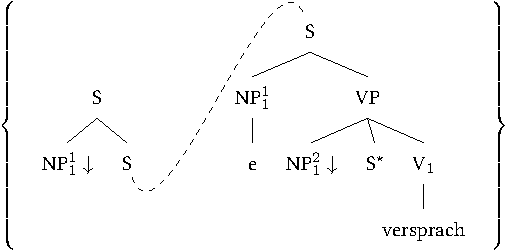
\includegraphics{Figures/tag-versprach-lsp-crop}
\caption{\label{Abbildung-MC-TAG-versprach}Elementary tree set for \emph{versprach} consisting of multiple components}
\end{figure}%
This tree contains a trace of NP$_1^1$ that was moved to the left. The bottom"=left S node and the top"=right S node are connected by a dashed line
that indicates the dominance relation. However, immediate dominance is not required. Therefore, it is possible to insert the two subtrees into another tree
separately from each other and thereby analyze the order in Figure~\vref{Abbildung-TAG-Permutation3}, for example.\is{Multi-Component TAG}\is{Tree Adjoining Grammar (TAG)!Multi"=Component (MC-TAG)|)} 
\begin{figure}
\centerline{%
\begin{forest}
tag
[S
	[NP$_1^1\downarrow$]
	[S
		[NP$_2^2\downarrow$]
		[S
			[NP$_1^1$
				[e]]
			[VP
				[NP$_1^2\downarrow$]
				[S
					[NP$_2^1\downarrow$]
					[S
						[NP
							[PRO]]
						[VP
							[NP$_2^1$
								[e]]
							[NP$_2^2$
								[e]]
							[V$_2$
								[zu überführen;to indict]]]]]
				[V$_1$
					[versprach;promised]]]]]]
\end{forest}
}
\caption{\label{Abbildung-TAG-Permutation3}Analysis of the order NP$_1^1$ NP$_2^2$ NP$_1^2$ NP$_2^1$ V$_{2}$V$_{1}$: adjunction to the S node between NP$_2^2$ and NP$_2^1$}
\end{figure}%

%Andere Varianten, die andere Konstituentenanordnungen zulassen sind V-TAG\is{Tree Adjoining Grammar@\emph{Tree Adjoining Grammar} (TAG)!\emph{Vektor} (V-TAG)} \citep{Rambow94a} und TT-MC-TAG\is{Tree Adjoining Grammar@\emph{Tree Adjoining Grammar} (TAG)!\emph{Tree Tuple MC-TAG} (TT-MC-TAG)} \citep{Lichte2007a}.\is{Konstituentenstellung|)}
Other variants of TAG that allow for other constituent orders are V-TAG\is{Tree Adjoining Grammar (TAG)!Vector (V-TAG)} \citep{Rambow94a} 
and TT-MC-TAG\is{Tree Adjoining Grammar (TAG)!Tree Tuple MC-TAG (TT-MC-TAG)} \citep{Lichte2007a}.\is{constituent order|)}

\section{Verb position}

%\largerpage
The position of the verb\is{verb position|(} can be analyzed in a parallel way to the GPSG analysis:
the verb can be realized in initial or in final position in a given linearization domain. Since the
verb position has an effect on the clause type and hence on semantics, a lexical rule"=based
analysis would be also viable: a tree with the finite verb in initial position is licensed by a
lexical rule that takes a tree with the verb in final position as input. This would be similar to
the analyses in GB, Minimalism, and HPSG.
\is{verb position|)}

\section{Passive}

There is\is{passive|(} a possible analysis for the passive that is analogous to the transformations in Transformational Grammar: one assumes lexical rules that
license a lexical item with a passive tree for every lexical item with an active tree \citep[\page 50--51]{KJ85a}. 

\citet[\page 55]{KJ85a} propose an alternative to this transformation"=like approach that more adequately handles so"=called raising constructions\is{raising}.
Their analysis assumes that arguments of verbs are represented in subcategorization lists. Verbs are entered into trees that match their subcategorization
list. Kroch and Joshi formulate a lexical rule that corresponds to the HPSG lexical rule that was discussed on page~\pageref{pass-lr-mlr}, that is,
an accusative object is explicitly mentioned in the input of the lexical rule. Kroch and Joshi then suggest a complex analysis of the impersonal passive which
uses a semantic null role for a non-realized object of intransitive verbs (p.\,56). Such an analysis
with abstract auxiliary entities can be avoided easily: one can instead use the HPSG\indexhpsg
analysis going back to \citet{Haider86}, which was presented in Section~\ref{Abschnitt-HPSG-Passiv}.
\largerpage

There\is{inheritance!multiple|(} are also proposals in TAG that use inheritance to deal with valence changing processes 
in general and the passive in particular (\citealp{Candito96a} and \citealp*{KSYJ2006a} following Candito). As we saw in Section~\ref{Abschnitt-Passiv-CxG} of 
the Chapter on Construction Grammar, inheritance is not a suitable descriptive tool for valence changing processes. This is because these kinds of processes
interact syntactically and semantically in a number of ways and can also be applied multiple times
(\citealp{Mueller2006d,Mueller2007d}; \citeyear[Section~7.5.2]{MuellerLehrbuch1};
\citeyear{MuellerUnifying}; \citeyear{MWArgSt}). See also Section~\ref{relations-sec} of this book.%
\is{inheritance!multiple|)}\is{passive|)}

\section{Long"=distance dependencies}
\label{TAG-Fernabh}

The\il{English|(}\is{long"=distance dependency|(} analysis of long"=distance dependencies in TAG is handled with the standard apparatus: simple trees are inserted
into the middle of other trees. Figure~\vref{abb-nld-TAG} shows an example of the analysis of (\mex{1}):
\ea
Who$_i$ did John tell Sam that Bill likes \_$_i$?
\z
%
\begin{figure}
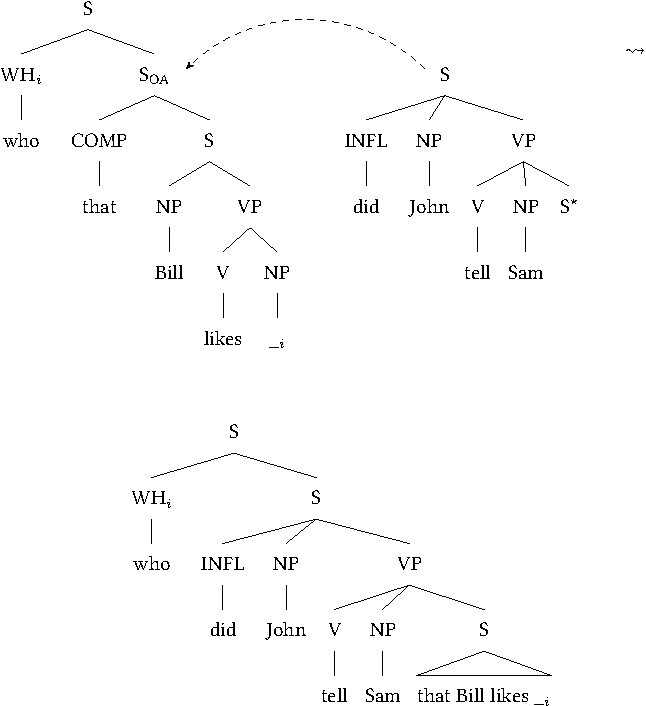
\includegraphics{Figures/tag-long-distance-dependencies-crop}
%%
%% Does not work with texlive 2015
%% %\oneline{%
%% \centerline{%
%% \begin{forest}
%% tag
%% [S
%% 	[WH$_i$
%% 		[who]]
%% 	[\tikzmark{soa}{S\sub{OA}}
%% 		[COMP
%% 			[that]]
%% 		[S
%% 			[NP
%% 				[Bill]]
%% 			[VP
%% 				[V
%% 					[likes]]
%% 				[NP
%% 					[\noexpand\_$_i$]]]]]]
%% \end{forest}
%% \hspace{0.5cm}
%% \begin{forest}
%% tag
%% [\tikzmark{s}{S}
%% 	[INFL
%% 		[did]]
%% 	[NP
%% 		[John]]
%% 	[VP
%% 		[V
%% 			[tell]]
%% 		[NP
%% 			[Sam]]
%% 		[S*]]]
%% \end{forest}
%% \qquad \raisebox{2cm}{$\rightsquigarrow$} \qquad
%% }\vspace{2\baselineskip}
%% \begin{forest}
%% tag
%% [S
%% 	[WH$_i$
%% 		[who]]
%% 	[S
%% 		[INFL
%% 			[did]]
%% 		[NP
%% 			[John]]
%% 		[VP
%% 			[V
%% 				[tell]]
%% 			[NP
%% 				[Sam]]
%% 			[S
%% 				[that Bill likes \noexpand\_$_i$, roof]]]]]
%% \end{forest}
%% \begin{tikzpicture}[overlay,remember picture]
%% \draw[->, dashed, bend angle=45, bend right] ($(pic cs:s)+(-0.25,0.2)$) to($(pic cs:soa)+(0.8,.2)$);
%%
%% \end{tikzpicture}
%%
%% {%\dotted
%% % todo \anodecurve[l]{s4}[tr]{s2}{0.1in}[3ex]%
%% }
%% \hspace{1ex}
%% $\leadsto$
%}
\caption{\label{abb-nld-TAG}Analysis of long"=distance dependencies in TAG}
\end{figure}%
The tree for \emph{WH COMP NP likes \_$_i$} belongs to the tree family of \emph{likes} and is therefore
present in the lexicon.
The tree for \emph{tell} is adjoined to this tree, that is, this tree is inserted in the middle of the tree for
\emph{who that Bill likes \_$_i$}. Such an insertion operation can be applied multiple times so that sentences such as (\mex{1})
where \emph{who} is moved across multiple sentence boundaries can be analyzed:
\ea 
Who$_i$ did John tell Sam that Mary said that Bill likes \_$_i$?
\z
%
There is another important detail: although the tree for (\mex{1}) has the category S, (\mex{1}) is not a grammatical
sentence of English.
\ea[*]{
who that Bill likes
}
\z
This has to be captured somehow. In TAG, the marking OA ensures that a tree counts as incomplete. If
a tree contains a node with marking OA, then an obligatory adjunction\is{adjunction!obligatory}
operation must take place at the relevant position.\il{English|)}\is{long"=distance dependency|)} 

\section{New developments and theoretical variants}

In Section~\ref{Abschnitt-MC-TAG}, we introduced Multi"=Component"=TAG. There are a large number of TAG variants with different formal properties.
\citet[\page
]{Rambow94a} gives an overview of the variants existing in 1994. In the following, I will discuss
two interesting variants of TAG: Feature Structure"=Based TAG (FTAG\indexftag, \citealp{VSJ88a}) and
Vector"=TAG (V"=TAG, \citealp{Rambow94a}). 

\subsection{FTAG}

In FTAG\is{Tree Adjoining Grammar (TAG)!Feature Structure"=Based (FTAG)|(}, nodes are not atomic (N,
NP, VP or S), but instead consist of feature descriptions. With the exception of substitution nodes, each node has a top structure and a bottom structure.
The top structure says something about what kind of properties a given tree has inside a larger structure, and the bottom structure says something
about the properties of the structure below the node.
Substitution nodes only have a top structure. Figure~\vref{Abbildung-FTAG-laughs} shows an example
tree for \emph{laughs}.\todostefan{geschwungenen Pfeil, alignierte Knoten}
\begin{figure}
\centerline{%
\begin{forest}
tag
[{\ms{
   cat & {\upshape S}\\
 }\\
\ms{
   cat & {\upshape S}
}}
  [\ms{
    cat & {\upshape NP}\\
    agr & \ibox{1}\\
   }
%
   [{[~]\\
    \ms{
       cat & {\upshape NP}\\
       agr & \ms{
              per & 3\\ 
              num & sing\\
             }\\
      }}, substitution,tier=2
      [John, tier=word] ] ]
  [{\ms{
     cat & {\upshape VP}\\
     agr & \ibox{1} \ms{
                    per & 3\\ 
                    num & sing\\
                    }\\
     }\\
     \ms{ 
     cat & {\upshape VP}\\
     }}
     [{\ms{
          cat & {\upshape V}\\
         }\\
       \ms{
          cat & {\upshape V}\\
       }}, tier=2
       [laughs,tier=word]]]
] 
\end{forest}
}
\caption{\label{Abbildung-FTAG-laughs}Elementary trees for \emph{John} and \emph{laughs} in FTAG}
\end{figure}%
A noun phrase can be combined with the tree for \emph{laughs} in Figure~\ref{Abbildung-FTAG-laughs}. Its top structure is identified with
the NP node in the tree for \emph{laughs}.
The result of this combination is shown in Figure~\vref{Abbildung-FTAG-John-laughs}.
\begin{figure}
\centerline{%
\begin{forest}
tag
[{\ms{
   cat & {\upshape S}\\
 }\\
\ms{
   cat & {\upshape S}
}}
  [{\ms{
    cat & {\upshape NP}\\
    agr & \ibox{1}\\
   }\\
    \ms{
       cat & {\upshape NP}\\
       agr & \ms{
              per & 3\\ 
              num & sing\\
             }\\
      }}
      [John, tier=word] ]
  [{\ms{
     cat & {\upshape VP}\\
     agr & \ibox{1} \ms{
                    per & 3\\ 
                    num & sing\\
                    }\\
     }\\
     \ms{ 
     cat & {\upshape VP}\\
     }}
     [{\ms{
          cat & {\upshape V}\\
         }\\
       \ms{
          cat & {\upshape V}\\
       }}
       [laughs,tier=word]]]
] 
\end{forest}
}
\caption{\label{Abbildung-FTAG-John-laughs}Combination of the trees for \emph{John} and \emph{laughs} in FTAG}
\end{figure}%

In a complete tree, all top structures are identified with the corresponding bottom structures. This way, only sentences where the subject is in
third person singular can be analyzed with the given tree for \emph{laughs}, that is, those in which
the verb's agreement features match those of the subject.

For adjunction, the top structure of the tree that is being inserted must be unifiable with the top structure of the adjunction site,
and the bottom structure of the node marked `*' in the inserted tree (the so"=called foot node\is{foot node}) must be unifiable with
the adjunction site.

The elementary trees discussed so far only consisted of nodes where the top part matched the bottom part. FTAG allows for an interesting variant of specifying 
nodes that makes adjunction obligatory\is{adjunction!obligatory|(}\label{page-feature-based-tag-oa} in order for the entire derivation to be well"=formed.
Figure~\vref{Obl-Adjunktion-FTAG} shows a tree for \emph{laughing} that contains two VP nodes with incompatible \textsc{mode} values.
\begin{figure}
\centerline{%
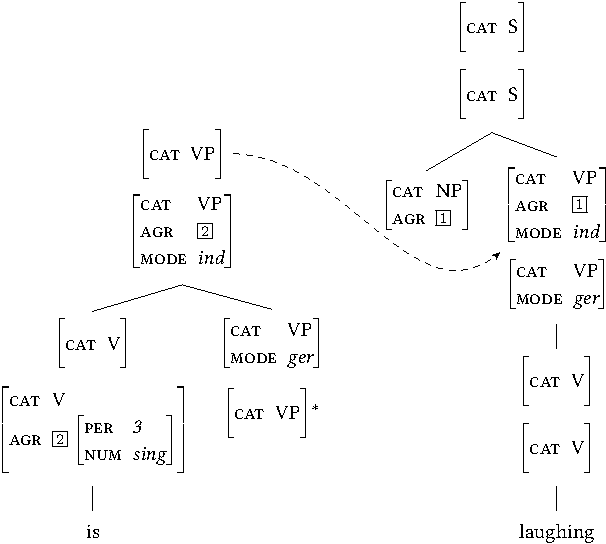
\includegraphics{Figures/tag-obl-adj-ftag-cropped}
}
% This does not work with texlive 2015 use texlive 2013
%% \hfill
%% \begin{forest}
%% [{\subnode{vpone}{\ms{
%%    cat & {\upshape VP}\\
%%  }}\vspace{2mm}\\ 
%%  \ms{
%%        cat & {\upshape VP}\\
%%        agr & \ibox{2}\\ 
%%        mode & ind\\
%%  }}
%%   [{\ms{
%%        cat & {\upshape V}\\
%%       }\vspace{2mm}\\
%%     \ms{
%%       cat & {\upshape V}\\
%%       agr & \ibox{2} \ms{
%%                       per & 3\\ 
%%                       num & sing\\
%%                      }\\
%%        }} [is]]
%%   [{\ms{
%%        cat & {\upshape VP}\\ 
%%        mode & ger\\
%%       }\vspace{2mm}\\
%%     \ms{
%%        cat & {\upshape VP}\\
%%        }$^*$}]]
%% \end{forest}
%% %% %%% sings tree:
%% %% \hspace{-1em}
%% \hfill
%% \begin{forest}
%% [{\ms{ 
%%    cat & {\upshape S}\\
%%  }\vspace{2mm}\\
%%  \ms{
%%   cat & {\upshape S}\\ 
%%   }}
%%   [\ms{ cat & {\upshape NP}\\
%%         agr & \ibox{1}\\
%%       }]
%%   [{\subnode{vptwo}{\ms{
%%       cat  & {\upshape VP}\\
%%       agr  & \ibox{1}\\
%%       mode & ind\\
%%       }}\vspace{2mm}\\
%%      \ms{
%%      cat & {\upshape VP}\\ 
%%      mode & ger\\
%%      }}
%%      [{\ms{ cat & {\upshape V}\\
%%           }\vspace{2mm}\\
%%        \ms{
%%             cat & {\upshape V}\\
%%         }}
%%        [laughing]]]]
%% \end{forest}
%% \hfill\mbox{}
%% \begin{tikzpicture}[overlay,remember picture,out=0,in=220]
%% \draw[->, dashed] (vpone) to (vptwo);
%% \end{tikzpicture}
\caption{\label{Obl-Adjunktion-FTAG}Obligatory adjunction in FTAG}
\end{figure}%
In order for this subtree to be used in a complete structure, another tree has to be added so that
the two parts of the VP node are separated. This happens
by means of an auxiliary tree as shown in Figure~\ref{Obl-Adjunktion-FTAG}. The highest VP node of the auxiliary tree is unified with the upper
VP node of \emph{laughing}. The node of the auxiliary tree marked with `*' is unified with the lower VP node of \emph{laughing}.
The result of this is given in Figure~\vref{Obl-Adjunktion-FTAG-Ergebnis}.
\begin{figure}
%%% is laughing tree:
\centerline{%
\begin{forest}
[{\ms{ 
   cat & {\upshape S}\\
 }\vspace{1mm}\\
  \ms{
   cat & {\upshape S}\\
  }}
  [{\ms{ cat & {\upshape NP}\\
         agr & \ibox{1}\\
   }}]
  [{\ms{
     cat  & {\upshape VP}\\
     agr  & \ibox{1}\\
     mode & ind\\
    }\vspace{1mm}\\
    \ms{
       cat & {\upshape VP}\\
       agr & \ibox{2}\\ 
       mode & ind\\
    }}
    [{\ms{
       cat & {\upshape V}\\
      }\vspace{1mm}\\
      \ms{
        cat & {\upshape V}\\
        agr & \ibox{2} \ms{
                per & 3\\ 
                num & sing\\
               }\\
         }} [is]]
     [{\ms{
        cat & {\upshape VP}\\ 
        mode & ger\\
      }\vspace{1mm}\\
      \ms{
       cat & {\upshape VP}\\ 
       mode & ger\\
      }}
      [{\ms{ cat & {\upshape V}\\
           }\vspace{1mm}\\
        \ms{
             cat & {\upshape V}\\
        }} [laughing]]]]]
\end{forest}
}
\caption{\label{Obl-Adjunktion-FTAG-Ergebnis}Result of obligatory adjunction in FTAG}
\end{figure}%

If a tree is used as a final derivation, the top structures are identified with the bottom structures. Thus, the \textsc{agr} value
of the highest VP node is identified with that of the lower one in the tree in Figure~\ref{Obl-Adjunktion-FTAG-Ergebnis}.
As such, only NPs that have the same \textsc{agr} value as the auxiliary can be inserted into the NP slot.

This example shows that, instead of the marking for obligatory adjunction\is{adjunction!obligatory|)} that we saw in the section on long"=distance
dependencies, the same effect can be achieved by using incompatible feature specifications on the top and bottom structures.
If there are incompatible top and bottom structures in a tree, then it cannot be a final derivation
tree and therefore this means that at least one adjunction operation must still take place in order
to yield a well"=formed tree.\is{Tree Adjoining Grammar (TAG)!Feature Structure"=Based (FTAG)|)}

\subsection{V"=TAG}
\label{sec-vtag}

V"=TAG\is{Tree Adjoining Grammar (TAG)!Vector (V-TAG)|(} 
is a variant of TAG proposed by Owen \citet{Rambow94a} that also assumes feature structures on
nodes. In addition, like MC"=TAG, it assumes that elementary trees consist of multiple components. Figure~\vref{Abbildung-Lexical-Set-geben-V-TAG} shows the elementary lexical set
for the ditransitive verb \emph{geben} `give'.
\begin{figure}
\vspace{4\baselineskip}
\menge{ 
\forestset{begin draw/.code={\begin{tikzpicture}[baseline=(current bounding box.center)]}}
    \hspace{1em}
    \begin{forest}
    [, phantom, for children={if n'=1{before computing xy={s*=1.25}}{}}
       %% This adjusts the relative position of the last child by zeroing its distance from the
       %% phantom root and increasing its distance from its sibling. This is delayed because 
       %% otherwise Forest will undo any changes when packing the tree.
      [VP
            [NP$\downarrow$]
            [VP, tikz+={\ignoreme\draw [densely dashed] ([yshift=2.5pt].south) [out=-75, in=-125] to ($(!u.north)!3/4!(!un.north)$) [out=55,in=100] to (!rl.north); }]]
    [VP
            [NP$\downarrow$]
            [VP, tikz+={\ignoreme\draw [densely dashed] ([yshift=2.5pt].south) [out=-75, in=-125] to ($(!u.north)!3/4!(!un.north)$) [out=55,in=100] to (!rl.north); }]]
    [VP
            [NP$\downarrow$]
            [VP, tikz+={\ignoreme\draw [densely dashed] ([yshift=2.5pt].south) [out=-75, in=-125] to ($(!u.north)!3/4!(!un.north)$) [out=55,in=100] to (!rl.north); }]]
    [VP
            [geben]
            [VP, tikz+={\ignoreme\draw [densely dashed] ([yshift=2.5pt].south) [out=-75, in=-125] to ($(!u.north)!3/4!(!un.north)$) [out=55,in=100] to (!rl.north); }]]
    [VP
            [$\epsilon$]]]
    \end{forest}
    \hspace{1em}
}
\vspace{.4\baselineskip}
\caption{\label{Abbildung-Lexical-Set-geben-V-TAG}Lexicon set for \emph{geben} `to give' in V"=TAG
  according to \citet[\page 6]{Rambow94a}}
\end{figure}%
\addlines
The lexicon set consists of a tree for the verb, an empty element of the category VP and three trees where a VP has been combined with
an NP. As in MC"=TAG, dominance relations are also indicated. The dominance constraints in Figure~\ref{Abbildung-Lexical-Set-geben-V-TAG}
ensure that all lower VP nodes dominate the highest VP node of the tree further to the right. The order of the arguments of the verb as
well as the position of the verb is not given. The only thing required is that lower VP in the NP
trees and lower VP in the \emph{geben} tree dominate the empty VP node.
With this lexicon set, it is possible to derive all permutations of the arguments. Rambow also shows
how such lexical entries can be used to analyze sentences with verbal complexes. Figure~\vref{Abbildung-zu-reparieren-versprochen-V-TAG} shows a verbal complex formed from
\emph{zu reparieren} `to repair' and \emph{versprochen} `promised' and the relevant dominance constraints.
\begin{figure}
\vspace{4\baselineskip}
\oneline{%
\menge{%
  \begin{forest}
    [, phantom, for children={if n'=1{before computing xy={l=0pt, s*=1.25}}{}}
       %% This adjusts the relative position of the last child (n'=1) by zeroing its distance from the
       %% phantom root (l=0) and increasing its distance from its sibling. This is delayed because 
       %% otherwise Forest will undo any changes when packing the tree.
      [VP
        [NP$\downarrow$]
        [VP, tikz+={\ignoreme\draw [densely dashed] ([yshift=2.5pt].south) [out=-75, in=-125] to
            ($(!u.north)!3/4!(!un.north)$) %[out=55,in=181]  to ++(4cm,2cm) [out=-1,in=90] 
            [out=55,in=90] to (!rll.north); }]
        % the following line is ignored for space computation due to \ignoreme
        % the first VP node at the baseline is connected to a place between the dominating vp !u.north and the node to the
        % left of it !un.north (the second VP node on the second line). 3/4 specifies the position
        % between these nodes. It is more to the second VP. From there we go to rll, which is the
        % root node's (r) last child's (l) last child (l). Since the root node is our phantom node,
        % the rll node is the last VP in the second row.
        %
        % the yshift raises the beginning of the line so that it is not too far away from the node.
      ]
      [VP
        [NP$\downarrow$]
        [VP, tikz+={\draw [densely dashed] ([yshift=2.5pt].south) [out=-80, in=180] to ++(20mm,-15mm) [out=0, in=-90] to ($(!unn.north)!.7!(!unnn1.north)$) [out=90, in=180] to ++(3.5mm,5mm) [out=0, in=90] to (!rl1.north); }]
      ]
      [VP
        [NP$\downarrow$]
        [VP, tikz+={\draw [densely dashed] ([yshift=2.5pt].south) [out=-80, in=180] to ++(10mm,-10mm) [out=0, in=-90] to ($(!un.north)!.6!(!unn1.north)$) [out=90, in=180] to ++(5.5mm,6.5mm) [out=0, in=90] to (!rl1.north); }]
      ]
      [VP
        [NP$\downarrow$]
        [VP, tikz+={\draw [densely dashed] ([yshift=2.5pt].south) [out=-80, in=-105] to ($(!u.north)!1/3!(!un.north)$) [out=75,in=90] to (!rll.north); }]
      ]
      [VP
        [VP
          [$\epsilon$]
          [zu reparieren]
        ]
        [VP, baseline
          [$\epsilon$]
          [versprochen]
        ]
      ]
    ]
  \end{forest}
}
}
\vspace{2.5\baselineskip}
\caption{\label{Abbildung-zu-reparieren-versprochen-V-TAG}Analysis of the verbal complex \emph{zu reparieren versprochen} in V"=TAG}
\end{figure}%%
Both of the first NP trees have to dominate \emph{versprochen} and the third and fourth NP tree have to dominate \emph{zu reparieren}.
The order of the NP trees is not restricted and thus all permutations of NPs can be derived.\pagebreak

The interesting thing here is that this approach is similar to the one proposed by \citet[Section~2.1.3]{Berman96a-u} in LFG\indexlfg
(see Section~\ref{Abschnitt-LFG-Umstellung}): in Berman's analysis, the verb projects directly to form a VP and the arguments are
then adjoined. 

A difference to other analyses discussed in this book is that there is always an empty
element\is{empty element} in the derived trees regardless
of verb position.%
\is{Tree Adjoining Grammar (TAG)!Vector (V-TAG)|)}

\subsection{The competence"=performance distinction and the generative capacity of tree"=local MC"=LTAG}
\label{Abschnitt-Kompetenz-Performanz-TAG}

In\is{competence|(}\is{performance|(} many of the theories discussed in this book, a distinction is made between competence and performance
\citep[Section~I.1]{Chomsky65a}. Competence theories are supposed to describe linguistic knowledge, whereas a performance theory should
explain how linguistic knowledge is used and why we make mistakes during speech production and
comprehension, etc. See Chapter~\ref{chap-competence-performance} for further discussion.

\citet*{JBR2000a} discuss examples of center self embedding of relative clauses as those in (\mex{1}b),
and follow \citet[\page 286]{CM63a}  in the assumption that the fact that this kind of embedding is only possible up to three levels should not be
described by grammar, but is rather due to processing problems with the hearer independent of their principle abilities with regard to grammar.
\eal
\label{TAG-Beispiel-Performanz}
\ex 
\gll dass der Hund bellt, der  die Katze jagt,  die  die Maus  gefangen hat\\
     that the dog  barks  that the cat   chases that the mouse caught   has\\
\glt `that the dog that chases the cat that caught the mouse barks'
\ex 
\gll dass der Hund, [$_1$ der  die Katze, [$_2$ die  die Maus  gefangen hat,~$_2$] jagt~$_1$] bellt\\
     that the dog   {}    that the cat    {}    that the mouse caught   has        chases    barks\\
\zl

\noindent
What is interesting in this context is that it is possible to construct examples of center embedding so that they are easier to process
for the hearer. In this way, it is possible to increase the number of center embeddings possible to
process by one and therefore to show that all grammars that formulate a restriction that there may
be at most two center"=embedded relative clauses are incorrect.
The following example from Hans Uszkoreit\aimention{Hans Uszkoreit} is easier to process since all embedded relative clauses are isolated and the verbs
are separated by material from the higher clause.
\ea
\gll Die Bänke, [$_1$ auf denen damals die Alten des Dorfes, [$_2$ die allen Kindern, [$_3$ die vorbeikamen $_3$], freundliche Blicke zuwarfen $_2$], 
lange Stunden schweigend nebeneinander saßen $_1$], mussten im letzten Jahr einem~~~~~~~ Parkplatz weichen.\\
the benches {} on which back.then the old.people of.the village {} that all children {} that came.by {} friendly glances gave {}
long hours silent next.to.each.other sat {} must in.the last year a car.park give.way.to\\
\glt `The benches on which the older residents of the village, who used to give friendly glances to all the children who came by, used to sit silently next to one 
another had to give way to a car park last year.'
\z
For other factors that play a role in processing, see \citew{Gibson98a}.

\addlines
\citet{JBR2000a} discuss verbal complexes with reordered arguments. The general pattern that they
discuss has the form shown in (\mex{1}):
\ea
$\sigma$(NP$_1$ NP$_2$ \ldots{} NP$_n$) V$_{n}$V$_{n-1}$ \ldots{} V$_{1}$
\z
Here, $\sigma$ stands for any permutation of noun phrases and V$_{1}$ is the finite verb.
The authors investigate the properties of Lexicalized Tree Adjoining Grammar (LTAG) with regard to this
pattern and notice that LTAG cannot analyze the order in (\mex{1}) if the semantics is supposed to
come out correctly.
\ea
NP$_2$ NP$_3$ NP$_1$ V$_{3}$V$_{2}$V$_{1}$
\z
Since (\mex{1}) is possible in German, LTAG is not sufficient to analyze all languages.
\ea
\gll dass ihm$_2$ das Buch$_3$ niemand$_1$ zu lesen$_3$ versprechen$_2$ darf$_1$\\
     that him     the book     nobody     to read      promise         be.allowed.to\\
\glt `that nobody is allowed to promise him to read the book' 
\z
Therefore, they propose the extension of TAG discussed in Section~\ref{Abschnitt-MC-TAG}; so"=called
\emph{tree"=local multi"=component LTAG} (Tree"=local MC"=LTAG or TL-MCTAG).
They show that TL-MCTAG can analyze (\mex{0}) but not (\mex{1}) with the correct semantics. They claim that these orders are not possible in German
and argue that in this case, unlike the relative clause examples, one has both options, that is, the
unavailability of such patterns can be explained as a performance phenomenon or as a
competence phenomenon.
\ea
\label{ex-mc-ltag-fails}
NP$_2$ NP$_4$ NP$_3$ NP$_1$ V$_{4}$V$_{3}$V$_{2}$V$_{1}$
\z
If we treat this as a performance phenomenon, then we are making reference to the complexity of the construction and the resulting processing problems
for the hearer. The fact that these orders do not occur in corpora can be explained with reference to the principle of cooperativeness\is{cooperativeness}.
Speakers normally want to be understood and therefore formulate their sentences in such a way that the hearer can understand them.
Verbal complexes in German with more than four verbs are hardly ever found since it is possible to simplify very complex sentences with multiple verbs in the 
right sentence bracket by extraposing\is{extraposition} material and therefore avoiding ambiguity\is{ambiguity} (see \citealp[\page 5]{Netter91} and
\citealp[\page 262]{MuellerLehrbuch1}).

The alternative to a performance explanation would involve using a grammatical formalism which is
just powerful enough to allow embedding of two verbs and reordering of their arguments, but rules
out embedding of three verbs and reordering of the arguments. \citet{JBR2000a} opt for this solution
and therefore attribute the impossibility of the order of arguments in (\mex{0}) to competence. 

In HPSG (and also in Categorial Grammar\indexcg and in some GB analyses\indexgb), verbal complexes are analyzed by means of argument composition
\citep{HN89b,HN94a}. Under this approach, a verbal complex behaves exactly like a simplex verb and the arguments of the verbs involved can be placed
in any order. The grammar does not contain any restriction on the number of verbs that can be combined, nor any constraints that ban embedding below a certain
level. In the following, I will show that many reorderings are ruled out by communication rules that
apply even with cases of simple two"=place verbs. The conclusion is that the impossibility of embedding four or more verbs should in fact be explained as a performance issue.

Before I present arguments against a competence"=based exclusion of (\ref{ex-mc-ltag-fails}), I will make a more general comment:
corpora cannot help us here since one does not find any instances of verbs with four or more embeddings. \citet{Bech55a} provides
an extensive collection of material, but had to construct the examples with four embedded verbs.
\citet[\page 94--95]{Meurers99c} gives constructed examples with five verbs that contain multiple auxiliaries or modal verbs.
These examples are barely processable and are not relevant for the discussion here since the verbs in (\ref{ex-mc-ltag-fails})
have to select their own arguments. There are therefore not that many verbs left when constructing examples. It is possible to only use subject
control verbs with an additional object (\eg \emph{versprechen} `to promise'), object control verbs (\eg \emph{zwingen} `to force')
or AcI verbs (\eg \emph{sehen} `to see' or \emph{lassen} `to let') to construct examples.
When constructing examples, it is important make sure that all the nouns involved differ as much as possible with regard to their
case\is{case} and their selectional restrictions\is{selection!restriction} (\eg animate/inanimate) since these are features that a hearer/reader could
use to possibly assign reordered arguments to their heads. If we want to have patterns such as (\ref{ex-mc-ltag-fails}) with four NPs each with a different
case, then we have to choose a verb that governs the genitive.
There are only a very small number of such verbs in German. Although the example constructed by \citet{JBR2000a} in (\ref{Beispiel-Joshi-NP4}) fulfills
these requirements, it is still very marked. It therefore becomes clear that the possibility of finding a corresponding example in a newspaper article
is extremely small. This is due to the fact that there are very few situations in which such an utterance would be imaginable. Additionally,
all control verbs (with the exception of \emph{helfen} `to help') require an infinitive with \emph{zu} `to' and can also be realized incoherently, that is,
with an extraposed infinitival complement without verbal complex formation. As mentioned above, a
cooperative speaker/""author would use a less complex construction and this reduces the probability
that these kinds of sentences arise even further.

Notice that tree"=local MC-LTAG does not constrain the number of verbs in a sentence. The formalism allows for an arbitrary number of verbs.
It is therefore necessary to assume, as in other grammatical theories, that performance constraints are responsible for the fact that we never find
examples of verbal complexes with five or more verbs. Tree"=local MC-LAG makes predictions about the possibility of arguments to be reordered.
I consider it wrong to make constraints regarding mobility of arguments dependent on the power of the grammatical formalism since the restrictions that
one finds are independent of verbal complexes and can be found with simplex verbs taking just two arguments.
The problem with reordering is that it still has to be possible to assign the noun phrases to the
verbs they belong to. If this assignment leads to ambiguity\is{ambiguity}
that cannot be resolved by case, selectional restrictions, contextual knowledge or intonation, then the unmarked constituent order is chosen.
\citet*[\page 68]{Hoberg81a} shows this very nicely with examples similar to the following:\footnote{        
        Instead of \emph{das} `the', Hoberg uses the possessive pronoun \emph{ihr} `her'.
		This makes the sentences more semantically plausible, but one then gets interference from the
		linearization requirements for bound pronouns. I have therefore replaced the pronouns with the definite article.
}
\eal
\judgewidth{\#}
\ex[]{
\gll Hanna hat immer schon gewußt, daß das Kind sie verlassen will.\\
	 Hanna has always already known that the child she leave wants\\
\glt `Hanna has always known that the child wants to leave her.'
}
\ex[\#]{
\gll Hanna hat immer schon gewußt, daß sie das Kind verlassen will.\\
     Hanna has always already known that she the child  leave wants\\
\glt Preferred reading: `Hanna has always known that she wants to leave the child.'
}
\ex[]{
  \raggedright
\gll Hanna hat immer schon gewußt, daß sie der Mann verlassen will.\\
     Hanna has always already known that she the.\nom{} man leave wants.to\\
\glt `Hanna has always known that the man wants to leave her.'
}
\zl
\pagebreak

\noindent
It is not possible to reorder (\mex{0}a)  to (\mex{0}b) without creating a strong preference for another reading.
This is due to the fact that neither \emph{sie} `she' nor \emph{das Kind} `the child' are unambiguously marked as
nominative or accusative. (\mex{0}b) therefore has to be interpreted as Hanna being the one that wants something, namely
to leave the child. This reordering is possible, however, if at least one of the arguments is unambiguously marked for case
as in (\mex{0}c).

For noun phrases with feminine count nouns, the forms for nominative and accusative as well as genitive and dative are the same.
For mass nouns, it is even worse. If they are used without an article, all cases are the same for feminine nouns (\eg \emph{Milch} `milk')
and also for masculines and neuters with exception of the genitive. In the following example from
\citet[\page 45]{Wegener85b} it is hardly possible to switch the dative and accusative object,
whereas this is possible if the nouns are used with articles as in (\mex{1}c,d): 

\eal
\ex 
\gll Sie mischt Wein Wasser bei.\\
     she mixes wine water into\\
\glt `She mixes water into the wine.'
\ex 
\gll Sie mischt Wasser Wein bei.\\
     she mixes water wine into\\
\glt `She mixes wine into the water.'
\ex 
\gll Sie mischt dem Wein das Wasser bei.\\
     she mixes the.\dat{} wine the.\acc{} water into\\
\glt `She mixes the water into the wine.'
\ex 
\gll Sie mischt das Wasser dem Wein bei.\\
	she mixes the.\acc{} water the.\dat{} wine into\\
\glt `She mixes the water into the wine.'
\zl
The two nouns can only be switched if the meaning of the sentence is clear from the context (\eg through explicit negation of the opposite)
and if the sentence carries a certain intonation.

The problem with verbal complexes is now that with four noun phrases, two of them almost always have the same case if one does not wish to
resort to the few verbs governing the genitive. A not particularly nice-sounding example of morphologically unambiguously marked case
is (\mex{1}):
\ea
\gll weil    er        den        Mann dem        Jungen des Freundes gedenken helfen lassen will\\
     because he.\nom{} the.\acc{} man  the.\dat{} boy    of.the.\gen{} friend remember help let wants\\
\glt `because he wants to let the man help the boy remember his friend'
\z
Another strategy is to choose verbs that select animate and inanimate objects so that animacy of the arguments can aid interpretation.
I have constructed such an example where the most deeply embedded predicate is not a verb but rather an adjective. The predicate \emph{leer fischen}
`to fish empty' is a resultative construction that should be analyzed parallel to verbal complexes \citep[Chapter~5]{Mueller2002b}.
\ea
\gll weil niemand$_1$ [den Mann]$_2$ [der Frau]$_3$ [diesen Teich]$_4$  leer$_4$ fischen$_3$ helfen$_2$ sah$_1$\\
     because nobody.\nom{} \spacebr{}the.\acc{} man \spacebr{}the.\dat{} woman \spacebr{}this.\acc{} pond empty fish help saw\\
\glt `because nobody saw the man help the woman fish the pond empty'
\z
If one reads the sentences with the relevant pauses, it is comprehensible. Case is unambiguously marked on the animate
noun phrases and our word knowledge helps us to interpret \emph{diesen Teich} `this pond' as the argument of \emph{leer} `empty'.  

The sentence in (\mex{0}) would correctly be analyzed by an appropriately written tree"=local MC-LTAG and also by argument composition
analyses for verbal complexes and resultative constructions. The sentence in (\mex{1}) is a variant of (\mex{0}) that corresponds exactly
to the pattern of (\ref{ex-mc-ltag-fails}):
\ea
\gll weil [der Frau]$_2$ [diesen Teich]$_4$ [den Mann]$_3$ niemand$_1$ leer$_4$ fischen$_3$ helfen$_2$ sah$_1$\\
	 because \spacebr{}the.\dat{} woman \spacebr{}this.\acc{} pond \spacebr{}the.\acc{} man nobody.\nom{} empty fish help saw\\
\glt `because nobody saw the man help the woman fish the pond empty'
\z
(\mex{0}) is more marked than (\mex{-1}), but this is always the case with local reordering (Gisbert Fanselow\aimention{Gisbert Fanselow}, p.\,c.\ 2006).
This sentence should not be ruled out by the grammar. Its markedness is more due to the same factors that were responsible for the markedness of reordering
of arguments of simplex verbs. Tree"=local MC-LTAG can not correctly analyze sentences such as (\mex{0}), which shows that this TAG variant is not
sufficient for analyzing natural language.

There are varying opinions among TAG researchers as to what should be counted as competence and what
should be counted as performance. For instance, \citet[\page 15]{Rambow94a} argues that one should
not exclude reorderings that cannot be processed by means of competence grammar or the grammatical
formalism. In Chapter~6, he presents a theory of performance that can explain why the reordering of
arguments of various verbs in the middle field is harder to process.
One should therefore opt for TAG variants such as V-TAG\is{Tree Adjoining Grammar (TAG)!Vector (V-TAG)} or TT-MC-TAG\is{Tree Adjoining Grammar (TAG)!Tree Tuple MC-TAG (TT-MC-TAG)} \citep{Lichte2007a} that are powerful enough to analyze the diverse reorderings
	and then also use a performance model that makes it possible to explain the gradual differences in acceptability.

An alternative to looking for a grammatical formalism with minimal expressive power is to not restrict the grammatical formalism at all with regard
to its expressive power and instead develop as restrictive linguistic theories as possible. For further discussion of this point, see 
Chapter~\ref{sec-generative-capacity}.
\is{competence|)}\is{performance|)}

\section{Summary and classification}

In sum, we have seen the following: LTAG is lexicalized, that is, there is at least one lexical element in every tree.
There are not any trees that correspond to the rule S $\to$ NP VP since no words are mentioned in this rule.
Instead, there are always complex trees that contain the subject NP and the VP. Inside the VP, there can be as much structure
as is necessary to ensure that the verb is contained in the tree. As well as the head, elementary trees in LTAG always contain
the arguments of the head. For transitive verbs, this means that both the subject and the object have to be components of the
elementary tree. This is also true of the trees used to analyze long"=distance dependencies. As shown in Figure~\ref{abb-nld-TAG},
the object must be part of the tree. The fact that the object can be separated from the verb by multiple sentence boundaries is not
represented in the elementary tree, that is, recursive\is{recursion} parts of grammar are not contained in elementary trees.
The relevant effects are achieved by adjunction, that is, by insertion of material into elementary trees.
The elementary tree for extraction in Figure~\ref{abb-nld-TAG} differs from the elementary tree for \emph{likes} given in
Figure~\ref{Abbildung-Max-likes-Anouk} for the use in normal SVO clauses. Every minimal construction, in which \emph{likes}
can occur (subject extraction, topicalization, subject relative clauses, object relative clauses, passive, \ldots) needs its own
elementary tree \citep[\page 10]{KJ2003a}. The different elementary trees can be connected using lexical rules\is{lexical rule}.
These lexical rules map a particular tree treated as underlying to other trees. In this way, it is possible to derive
a passive tree from an active tree. These lexical rules are parallel to transformations\is{transformation} in Transformational
Grammar, however, one should bear in mind that there is always a lexical element in the tree, which makes the entire grammar
more restrictive than grammars with free transformations.

An interesting difference to GB and variants of LFG, CG, and HPSG that assume empty elements\is{empty element} is that
the variants of TAG presented here\footnote{
	See \citew{Rambow94a} and \citew[\page 194]{Kallmeyer2005a-u}, however, for TAG analyses with an empty element in the lexicon.%
} do not contain empty elements in the lexicon. They can be used in trees but trees are listed as a whole in the lexicon.

Elementary trees can be of any size, which makes TAG interesting for the analysis of idioms (see Section~\ref{Abschnitt-Diskussion-Lokalitaet}). 
Since recursion is factored out, trees can contain elements that appear very far away from each other in
the derived tree (extended domains of locality\is{locality}).

\citet*{KKNV95a} show that it is possible to transfer HPSG grammars that fulfill certain requirements into TAG grammars. This is interesting
as in this way one arrives at a grammar whose complexity behavior is known\is{capacity!generative}. Whereas HPSG grammars are generally
in the Type-0 area, TAG grammars can, depending on the variant, fall into the realm of Type-2 languages (context"=free) or even in the
larger set of the mildly context"=sensitive grammars\is{mildly context"=sensitive grammar!context"=sensitive grammar} \citep{Joshi85a-u}. \citet*{YMTT2001a} have developed a procedure for translating FB"=LTAG grammars into
HPSG grammars.


\section*{Comprehension questions}

\begin{enumerate}
\item How are long"=distance dependencies analyzed in TAG? Does one need empty elements for this?
\item Is it possible to analyze the reordering of arguments of multiple verbs using standard TAG processes?
\end{enumerate} 

\section*{Exercises}

\begin{enumerate}
\item Analyze the following string in LTAG:
\ea
\gll der dem König treue Diener\\
	 the the.\dat{} king loyal servant\\
\glt `the servant loyal to the king'
\z
\end{enumerate}

\section*{Further reading}

Some important articles are \citew*{JLT75a-u}, \citew{Joshi87a-u}, and \citew{JS97a}. Many works discuss formal properties of TAG and are therefore not particularly accessible for
linguistically interested readers. \citew{KJ85a} give a good overview of linguistic analyses. An overview of linguistic and computational linguistic
works in TAG can be found in the volume edited by Abeill{\'e} and
Rambow\nocite{AR2000a-ed-not-crossreferenced} from 2000. \citet{Rambow94a} compares his TAG variant (V"=TAG\is{Tree
  Adjoining Grammar (TAG)!Vector (V-TAG)}) to Karttunen's \emph{Radical Lexicalism} approach, Uszkoreit's GPSG\indexgpsg,
Combinatorial Categorial Grammar\indexcg, HPSG\indexhpsg and
Dependency Grammar\indexdg. 

\citet{SJ93a} discuss psycholinguistically plausible processing models and show that it is possible to do incremental parsing with TAG. They also present a
further variant of TAG: synchronous TAG\indexstag. In this TAG variant, there is a syntactic tree and a semantic tree connected to it.
When building syntactic structure, the semantic structure is always built in parallel. This structure built in parallel corresponds to the level of Logical
Form\is{Logical Form (LF)} derived from S"=Structure\is{S"=Structure} using transformations\is{transformation} in GB.


\citet[Chapter~6]{Rambow94a} presents an automaton"=based performance theory. He applies it to German and shows that
the processing difficulties that arise when reordering arguments of multiple verbs can be explained.
\is{Tree Adjoining Grammar (TAG)|)}

\citet{KR2008a-u} show how it is possible to derive MRS representations directly via a derivation tree using FTAG. In each top node, there is a reference
to the semantic content of the entire structure and each bottom node makes reference to the semantic content below the node. In this way, it becomes possible
to insert an adjective (\eg \emph{mutmaßlichen} `suspected') into an NP tree \emph{alle Mörder} `all murderers' so that the adjective has scope over
the nominal part of the NP (\emph{Mörder} `murderers'): for adjunction of the adjective to the N node, the adjective can access the semantic content of the noun.
The top node of \emph{mutmaßlichen} is then the top node of the combination \emph{mutmaßlichen Mörder} `suspected murderers' and this ensures that the meaning of \emph{mutmaßlichen Mörder}
is correctly embedded under the universal quantifier.


%      <!-- Local IspellDict: en_US-w_accents -->

\include{chapters/ot}

\part{General discussion}\label{part-discussion}

%% -*- coding:utf-8 -*-
\exewidth{(235)}%

\chapter{The innateness of linguistic knowledge}
\label{Abschnitt-Angeborenheit}\label{chap-innateness}
%
% Haspelmath2010c:391 tendencies


If we try and compare the theories presented in this book, we notice
that there are a number of similarities.\footnote{\label{fn-ffs}%
  The terms \emph{theory} and \emph{framework} may require clarification. A framework is a common
  set of assumptions and tools that is used when theories are formulated. In this book, I discussed
  theories of German. These theories were developed in certain frameworks (GB, GPSG, HPSG, LFG, \ldots) and of course there are
  other theories of other languages that share the same fundamental assumptions. These theories
  differ from the theories of German presented here but are formulated in the same
  framework. \citet{Haspelmath2010c} argues for framework-free grammatical theory. If grammatical
  theories used incompatible tools, it would be difficult to compare languages. So assuming
  transformations for English nonlocal dependencies and a \slasch mechanism for German would make
  comparison impossible. I agree with Haspelmath that the availability of formal tools may lead to
  biases, but in the end the facts have to be described somehow. If nothing is shared between
  theories, we end up with isolated theories formulated in one man frameworks. If there \emph{is} shared
  vocabulary and if there are standards for doing framework"=free grammatical theory, then the
  framework is framework"=free grammatical theory. See
  \citet{MuellerCoreGram} and Chapter~\ref{Abschnitt-UG-mit-Hierarchie} of this book for further discussion.
}
In all of the frameworks, there are variants of theories that use feature"=value pairs to describe linguistic objects.
The syntactic structures assumed are sometimes similar. Nevertheless, there are some differences that have often led to fierce debates
between members of the various schools. Theories differ with regard to whether they assume transformations, empty elements, phrasal or lexical analyses,
binary branching or flat structures.

Every theory has to not only describe natural language, but also explain it. It is possible to
formulate an infinite number of grammars that license structures for a given language (see Exercise~\ref{ua-psg-eins} on page~\pageref{ua-psg-eins}). These grammars are \emph{observationally adequate}\is{observational adequacy}.
A grammar achieves \emph{descriptive adequacy}\is{descriptive adequacy} if it corresponds to observations and the intuitions of native speakers.\footnote{
This term is not particularly useful as subjective factors play a role. Not everybody finds grammatical theories intuitively correct where it is assumed that every
observed order in the languages of the world has to be derived from a common
Specifier"=Head"=Complement configuration, and also only by movement to the left (see Section~\ref{Abschnitt-Kaynesche-Modelle} for the discussion of such proposals).
}
A linguistic theory is descriptively adequate if it can be used to formulate a descriptively adequate grammar for every natural language. However, grammars achieving descriptive
adequacy do not always necessarily reach \emph{explanatory adequacy}\is{explanatory adequacy}. Grammars that achieve explanatory adequacy are those that are compatible with
acquisition data\is{language acquisition}, that is, grammars that could plausibly be acquired by human speakers \citep[\page
  24--25]{Chomsky65a}.

\citet[\page 25]{Chomsky65a} assumes that children already have domain"=specific knowledge about what grammars could, in principle, look like and then extract information about what
a given grammar actually looks like from the linguistic input. The most prominent variant of acquisition theory in Mainstream Generative Grammar (MGG) is the Principles \& Parameters
theory, which claims that parametrized principles restrict the grammatical structures possible and
children just have to set parameters during language acquisition
(see Section~\ref{Abschnitt-GB-Paramater}).

Over the years, the innateness hypothesis, also known as nativism\is{nativism}, has undergone a number of modifications.
In particular, assumptions about exactly what forms part of the innate linguistic knowledge,
so"=called Universal Grammar (UG)\is{Universal Grammar (UG)}, have often been subject to change.

Nativism is often rejected by proponents of Construction Grammar\indexcxg, Cognitive
Grammar\is{Cognitive Grammar} and by many other researchers working in other theories. Other
explanations are offered for the facts normally used to argue for the innateness of grammatical
categories, syntactic structures or relations between linguistic objects in syntactic structures.
Another point of criticism is that the actual complexity of analyses is blurred by the fact that many of the stipulations are simply assumed to be part of UG.
The following is a caricature of a certain kind of argumentation in GB/Minimalism analyses: 

\begin{enumerate}
\item I have developed an analysis for the phenomenon P in the language S.
\item The analysis is elegant/conceptually simple/mine\footnote{
    Also, see
    \url{http://www.youtube.com/watch?v=cAYDiPizDIs}. 01.12.2015.\nocite{Zappa86a}\aimention{Frank Zappa}
}.
\item There is no possibility to learn the relevant structures or principles.
\item Therefore, the assumptions A$_1$ through A$_n$ that are made in this analysis must be part of the innate knowledge
of speakers.
\end{enumerate}
By attributing arbitrary assumptions to UG, it is possible to keep the rest of the analysis very
simple.

The following section will briefly review some of the arguments for language"=specific innate knowledge.
We will see that none of these arguments are uncontroversial. In the following chapters, I will discuss fundamental
questions about the architecture of grammar, the distinction between competence and performance and how to model
performance phenomena, the theory of language acquisition as well as other controversial questions, \eg 
whether it is desirable to postulate empty elements in linguistic representations and whether language should
be explained primarily based on the properties of words or rather phrasal patterns.

Before we turn to these hotly debated topics, I want to discuss the one that is most fiercely
debated, namely the question of innate linguistic knowledge. In the literature, one finds the
following arguments for innate knowledge:

\begin{itemize}
\item the existence of syntactic universals,
\item the speed of acquisition,
\item the fact that there is a `critical period' for language acquisition,
\item the fact that all children learn a language, but primates do not,
\item the fact that children spontaneously regularize pidgin languages, 
\item the localization of language processing in particular parts of the brain,
\item the alleged dissociation of language and general cognition:
\begin{itemize}
\item Williams Syndrome,
\item the KE family with FoxP2 mutation and
\end{itemize}
\item the Poverty of the Stimulus Argument.
\end{itemize}
\citet{Pinker94a} offers a nice overview of these arguments. \citet{Tomasello95a} provides a critical review of this book. The individual points will be discussed in what follows.

\section{Syntactic universals}
\label{sec-syntactic-universals}

The\is{universal|(} existence of syntactic universals has been taken as an argument for the innateness of linguistic knowledge
(\eg \citealp[\page 33]{Chomsky98a-u}; %\citealp[\page 46--47]{Chomsky88a-u}; %\citealp[\page 46--47]{Chomsky88a}, ist in Stanford falsch zitiert
\citealp[\page 237--238]{Pinker94a}). There are varying claims in the literature with regard to what is universal and 
language"=specific. The most prominent candidates for universals are:\footnote{
Frans Plank\aimention{Frans Plank} has an archive of universals in Konstanz \citep{PF2000a}:
\url{http://typo.uni-konstanz.de/archive/intro/}. On 23.12.2015, it contained 2029 entries.
The entries are annotated with regard to their quality, and it turns out that many of the universals
are statistical universals, that is, they hold for the overwhelming majority of languages, but there are
some exceptions. Some of the universals are marked as almost absolute, that is, very few exceptions are known.
1153 were marked as absolute or absolute with a question mark. 1021 of these are marked as absolute without
a question mark. Many of the universals captured are implicational universals\is{universal!implicational}, that is, they have the form:
if a language has the property X, then it also has the property Y. The universals listed in the archive
are, in part, very specific and refer to the diachronic development of particular grammatical
properties. For example, the fourth entry states that: \emph{If the exponent of
  vocative is a prefix, then this prefix has arisen from 1st person possessor or a 2nd person
  subject.} 
}\nocite{Harbour2011a}

\begin{itemize}
\item the Head Directionality Parameter
\item \xbar structures
\item grammatical functions such as subject or object
\item binding principles
\item properties of long"=distance dependencies
\item grammatical morphemes for tense, mood and aspect
\item parts of speech
\item recursion or self"=embedding
\end{itemize}

\noindent
These supposed universals will each be discussed briefly in what follows. One should emphasize that there is by no means
a consensus that these are universal and that the observed properties actually require postulating innate linguistic
knowledge.

\subsection{Head Directionality Parameter}
\label{Abschnitt-Kopfstellungsparameter}

% a month ago -> head final
% counterexamples notwithstanding
\mbox{}\is{parameter!head direction|(}%
The Head Directionality Parameter was already introduced in Section~\ref{Abschnitt-GB-Paramater}. The examples in (\ref{Bsp-Kopfstellungsparameter}) on
page~\pageref{Bsp-Kopfstellungsparameter}, repeated below as (\mex{1}), show that the structures in Japanese are the mirror image of the English structures:
\eal
\label{Bsp-Kopfstellungsparameter-zwei}
\ex 
be showing pictures of himself
\ex
\gll zibun  -no syasin-o mise-te iru\\
     himself \hspaceThis{-}of picture showing be\\
\zl
In order to capture these facts, a parameter was proposed that is responsible for the position of the head relative to its
arguments (\eg Chomsky \citeyear[\page 146]{Chomsky86}; \citeyear[\page 70]{Chomsky88a-u}). 

By assuming a Head Directionality Parameter, Radford (\citeyear[\page 60--61]{Radford90a-u}; \citeyear[\page 19--22]{Radford97a-u}), \citet[\page 234, 238]{Pinker94a}, \citet[\page 350]{Baker2003b}
and other authors claim, either explicitly or implicitly, that there is a correlation between the direction of government of verbs and that of adpositions, that is, languages
with verb"=final order have postpositions and languages with VO order have prepositions. This claim
can be illustrated with the language pair English\il{English}/""Japanese\il{Japanese} and the
examples in (\mex{0}): the \emph{no} occurs after the pronoun in the prepositional phrase, the noun \emph{syasin-o} `picture' follows the PP belonging to it, the main verb follows its object and the
auxiliary \emph{iru} occurs after the main verb \emph{mise-te}. The individual phrases are the exact mirror image of
the respective phrases in English.

\addlines[2]
A single counterexample is enough to disprove a universal  claim and in fact, it is possible to
find a language that has verb"=final order but nevertheless has prepositions.
Persian\il{Persian} is such a language. An example is given in (\mex{1}):
\ea
\gll man ketâb-â-ro be Sepide dâd-am.\\
     I book-\pl-\RA{} to Sepide gave-1\sg\\
\glt `I gave the books to Sepide.'
\z
In Section~\ref{Abschnitt-X-Bar}, it was shown that German cannot be easily described with this parameter: German is a verb"=final language but has both
prepositions and postpositions. The World Atlas of Language Structures lists 41 languages with VO
order and postpositions and 14 languages with OV order and prepositions \citep{wals-83,wals-85}.\footnote{
  \url{http://wals.info/combinations/83A_85A\#2/15.0/153.0}, 23.12.2015.
} An earlier study by \citet{Dryer92a} done with a smaller sample of languages also points out that
there are exceptions to what the Head Directionality Parameter would predict. 

Furthermore, \citet[\page 422]{GW94a} point out that a single parameter for the position of heads would not be enough since complementizers in both English and German/Dutch
occur before their complements; however, English is a VO language, whereas German and Dutch count as OV languages.

If one wishes to determine the direction of government based on syntactic categories (\citealp[\page 422]{GW94a}, \citealp[\page 15]{Chomsky2005a}), then one has to assume
that the syntactic categories in question belong to the inventory of Universal Grammar (see Section~\ref{Abschnitt-UG-Wortarten}, for more on this).
Difficulties with prepositions and postpositions also arise for this kind of assumption as these are normally assigned to the same category (P).
If we were to introduce special categories for both prepositions and postpositions, then a four"=way
division of parts of speech like the one on page~\pageref{Tabelle-Merkmalszerlegung-Wortarten} would
no longer be possible. One would instead require an additional binary feature and one would thereby
automatically predict eight categories although only five (the four commonly assumed plus an extra one) are actually needed.

One can see that the relation between direction of government that Pinker formulated as a universal
claim is in fact correct but rather as a tendency than as a strict rule, that is, there are many languages where
there is a correlation between the use of prepositions or postpositions and the position the verb
\citep[\page 83]{Dryer92a}.\footnote{
\citet[\page 234]{Pinker94a} uses the word \emph{usually} in his formulation. He thereby implies
that there are exceptions and that the correlation between the ordering of adpositions and the
direction of government of verbs is actually a tendency rather than
a universally applicable rule. However, in the pages that follow, he argues that the Head Directionality Parameter forms part of innate linguistic knowledge.
\citet[\page 55]{Travis84a-u} discusses data from Mandarin Chinese that do not correspond to the correlations she assumes. She then proposes treating the Head Directionality Parameter
as a kind of Default Parameter that can be overridden by other constraints in the language.
} 

In many languages, adpositions have evolved from verbs. In Chinese\is{Mandarin Chinese} grammar, it is commonplace to refer to a particular class of words as coverbs\is{coverb}.
These are words that can be used both as prepositions and as verbs. If we view languages historically, then we can find explanations for these tendencies that do not have to make
reference to innate linguistic knowledge (see \citealp[\page 445]{EL2009a}). 

Furthermore, it is possible to explain the correlations with reference to processing preferences: in languages with the same direction of government, the distance between the verb
and the pre-/postposition is less (Figure~\ref{fig-head-position}a--b) than in languages with
differing directions of government (Figure~\ref{fig-head-position}c--d).
\begin{figure}
\hfill
%\begin{tabular}{cc}
\subfloat[SVO with prepositions (common)]{
\makebox[.4\textwidth]{
\begin{tikzpicture}
\tikzset{level 1+/.style={level distance=2\baselineskip}}
%\tikzset{frontier/.style={distance from root=24\baselineskip}}
\Tree[.IP NP
       [.VP \node(v){V}; NP [.PP \node(p){P}; NP ] 
       ]
]
\draw (v) |-  ([yshift=-5mm]v |- p) -| (p);
\end{tikzpicture}}}
\hfill
\subfloat[SOV with postpositions (common)]{
\makebox[.4\textwidth]{
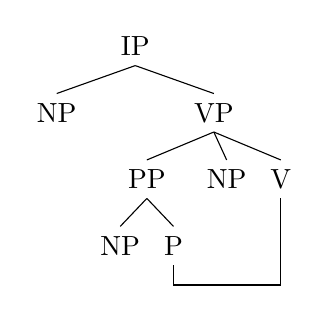
\begin{tikzpicture}
\tikzset{level 1+/.style={level distance=2\baselineskip}}
%\tikzset{frontier/.style={distance from root=24\baselineskip}}
\Tree[.IP NP
       [.VP [.PP NP \node(p){P}; ] NP \node(v){V};
       ]
]
\draw (v) |-  ([yshift=-5mm]v |- p) -| (p);
\end{tikzpicture}}}\hfill\mbox{}

\hfill
\subfloat[SVO with postpositions (rare)]{
\makebox[.4\textwidth]{
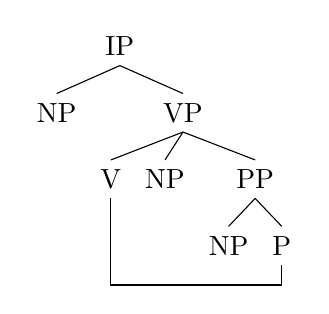
\begin{tikzpicture}
\tikzset{level 1+/.style={level distance=2\baselineskip}}
%\tikzset{frontier/.style={distance from root=24\baselineskip}}
\Tree[.IP NP
       [.VP \node(v){V}; NP [.PP NP \node(p){P}; ] 
       ]
]
\draw (v) |-  ([yshift=-5mm]v |- p) -| (p);
\end{tikzpicture}}}
\hfill
\subfloat[SOV with prepositions (rare)]{
\makebox[.4\textwidth]{
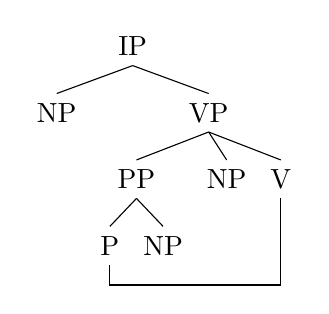
\begin{tikzpicture}
\tikzset{level 1+/.style={level distance=2\baselineskip}}
%\tikzset{frontier/.style={distance from root=24\baselineskip}}
\Tree[.IP NP
       [.VP [.PP \node(p){P}; NP ] NP \node(v){V};
       ]
]
\draw (v) |-  ([yshift=-5mm]v |- p) -| (p);
\end{tikzpicture}}}
\hfill\mbox{}
\caption{Distance between verb and preposition for various head orders according to \citet[\page 221]{Newmeyer2004b}}\label{fig-head-position}
\end{figure}%
From the point of view of processing, languages with the same direction of government should be preferred since they allow the hearer to better identify the parts
of the verb phrase (\citet[\page 219--221]{Newmeyer2004b} cites \citew[\page 32]{Hawkins2004a-u}
with a relevant general processing preference, see also \citew[\page 131]{Dryer92a}). This tendency can thus be explained as the
grammaticalization of a performance preference (see Chapter~\ref{Abschnitt-Diskussion-Performanz}
for the distinction between competence and performance) and recourse to innate language"=specific
knowledge is not necessary.%
\is{parameter!head direction|)}

\subsection{\xbar structures}
\label{sec-Diskussion-X-Bar}

It\is{X theory@\xbar theory|(} is often assumed that all languages have syntactic structures that
correspond to the \xbar schema (see Section~\ref{sec-xbar}) (\citealp[\page
238]{Pinker94a}; \citealp[\page 11, 14]{Meisel95a}; \citealp[\page 216]{PJ2005a}). There are, however, languages such as Dyirbal\il{Dyirbal} (Australia) where it does not seem
to make sense to assume hierarchical structure for sentences.
Thus, \citet[\page 110]{Bresnan2001a} assumes that Tagalog\il{Tagalog}, Hungarian\il{Hungarian},
Malayalam\il{Malayalam}, Warlpiri\il{Warlpiri}, Jiwarli\il{Jiwarli}, Wambaya\il{Wambaya},
Jakaltek\il{Jakaltek}
and other corresponding languages do not have a VP node, but rather a rule taking the form of (\mex{1}): 
\ea
S $\to$ C$^*$
\z
Here, C$^*$ stands for an arbitrary number of constituents and there is no head in the structure.
Other examples for structures without heads will be discussed in Section~\ref{Abschnitt-Phrasale-Konstruktionen}.

\addlines
\xbar structure was introduced to restrict the form of possible rules. The assumption was that these restrictions reduce the class
of grammars one can formulate and thus -- according to the assumption -- make the grammars easier to
acquire. But as \citet{KP90a} have shown,
the assumption of \xbar structures does not lead to a restriction with regard to the number of possible grammars if one allows for empty heads\is{empty element}.
In GB, a number of null heads were used and in the Minimalist Program\indexmp, there has been a
significant increase of these. For example, the rule in (\mex{0}) can be reformulated as follows:
\ea
V$'$ $\to$ \vnull C$^*$
\z
Here, \vnull is an empty head. Since specifiers are optional, V$'$ can be projected to VP and we arrive at a structure corresponding to
the \xbar schema.

Apart from the problem with languages with very free constituent order, there are further problems with adjunction structures: Chomsky's analysis of adjective structure
in \xbart (\citealp[\page 210]{Chomsky70a}; see also Section~\ref{sec-xbar} of this book, in
particular Figure~\vref{Abbildung-AP}) is not straightforwardly applicable to German since, unlike
English, adjective phrases in German are head"=final and degree modifiers must directly precede the
adjective: 
\eal
\ex[]{
\gll der auf seinen Sohn sehr stolze Mann\\
	 the of his son very proud man\\
\glt `the man very proud of his son'
}
\ex[*]{
\gll der sehr auf seinen Sohn stolze Mann\\
	 the very of his son proud man\\
}
\ex[*]{
\gll der auf seinen Sohn stolze sehr Mann\\
	 the of his son proud very man\\
}
\zl
Following the \xbar schema, \emph{auf seinen Sohn} has to be combined with \emph{stolze} and only then can the
resulting \abar projection be combined with its specifier (see Figure~\vref{Abbildung-AP} for the structure of adjective
phrases in English). It is therefore only possible to derive orders such as (\mex{0}b) or (\mex{0}c). Neither of these
is possible in German. It is only possible to rescue the \xbar schema if one assumes that German is
exactly like English and, for some reason, the complements of adjectives must be moved to the left. If we allow this kind of repair
approaches, then of course any language can be described using the \xbar schema. The result would be that one would have
to postulate a vast number of movement rules for many languages and this would be extremely complex and difficult
to motivate from a psycholinguistic perspective. See Chapter~\ref{Abschnitt-Diskussion-Performanz} for grammars compatible with performance.

A further problem for \xbart in its strictest form as presented in Section~\ref{sec-xbar} is posed by so"=called hydra clauses\is{hydra clause} \citep{PR70a,Link84a-u,Kiss2005a}:
\eal
\ex {}
\gll [[der Kater] und [die Katze]], die einander lieben\\
     \spacebr{}\spacebr{}the tomcat and the cat that each.other love\\
\glt `the tomcat and the (female) cat that love each other'
\ex {}[[The boy] and [the girl]] who dated each other are friends of mine. 
\zl
Since the relative clauses in (\mex{0}) refer to a group of referents, they can only attach to the result of the coordination.
The entire coordination is an NP, however, and adjuncts should actually be attached at the \xbar level. The reverse case of relative clauses
in German and English is posed by adjectives in Persian: \citet{Samvelian2007a} argues for an analysis where adjectives are combined with nouns
directly, and only the combination of nouns and adjectives is then combined with a PP argument.

The discussion of German and English shows that the introduction of specifiers and adjuncts cannot be restricted to particular projection levels, and
the preceding discussion of non"=configurational languages has shown that the assumption of intermediate levels does not make sense for every language.

It should also be noted that Chomsky himself assumed in 1970 that languages can deviate from the \xbar
schema \citeyearpar[\page 210]{Chomsky70a}.

If one is willing to encode all information about combination in the lexicon, then one could get by with very abstract combinatorial rules that would hold universally.
An example of this kind of combinatorial rules is the multiplication rules of Categorial Grammar\is{Categorial Grammar (CG)} (see Chapter~\ref{Kapitel-CG}) 
as well as Merge\is{Merge} in the Minimalist Program\indexmp (see Section~\ref{Abschnitt-MP}).
The rules in question simply state that two linguistic objects are combined. These kinds of
combination of course exist in every language. With completely lexicalized grammars, however, it is only possible to describe languages
if one allows for null heads and makes certain ad hoc assumptions. This will be discussed in
Section~\ref{Abschnitt-Phrasale-Konstruktionen}.\is{X theory@\xbar theory|)} 

\subsection{Grammatical functions such as subject and object}
\label{Abschnitt-UG-EPP}

\addlines[2]
\mbox{}\citet[\page xxv]{BK82a}, \citet[\page 236--237]{Pinker94a}\is{subject|(}\is{object|(}\is{grammatical function|(}, \citet[\page 349]{Baker2003b} 
and others assume that all languages have subjects and objects. In order to determine what exactly this claim means, we have to explore the terms
themselves. For most European languages, it is easy to say what a subject and an object is (see Section~\ref{Abschnitt-GF}); however,
it has been argued that it is not possible for all languages or that it does not make sense to use
these terms at all (\LATER{\citealp{Durie85a}; }\citealp[Chapter~4]{Croft2001a}; \citealp[Section~4]{EL2009a}).

In theories such as LFG\indexlfg{} -- the one in which Pinker worked -- grammatical functions play a primary role. The fact that it is still
controversial whether one should view sentences as subjects, objects or as specially defined sentential arguments (\xcomp) \citep*{DL2000a-u,Berman2003a-u,Berman2007a-u,AMM2005a-u,Forst2006a-u}
serves to show that there is at least some leeway for argumentation when it comes to assigning
grammatical functions to arguments. It is therefore likely that one can find an assignment of
grammatical functions to the arguments of a functor in all languages. 

Unlike LFG, grammatical functions are irrelevant in GB (see \citealp{Williams84a,Sternefeld85a}) and Categorial Grammar\indexcg. In GB, grammatical functions can only be
determined indirectly by making reference to tree positions. Thus, in the approach discussed in
Chapter~\ref{Kapitel-GB}, the subject is the phrase in the specifier position of IP.

In later versions of Chomskyan linguistics, there are functional nodes that seem to correspond to grammatical functions (AgrS\is{category!functional!AgrS},
AgrO\is{category!functional!AgrO}, AgrIO\is{category!functional!AgrIO}, see
page~\pageref{Seite-AgrO}). However, \citet[Section~4.10.1]{Chomsky95a-u} remarks that these functional categories were only assumed for theory internal reasons
and should be removed from the inventory of categories that are assumed to be part of UG. See \citew{Haider97a} and \citew[\page 509--510]{Sternefeld2006a-u} for a description of German that does without functional projections
that cannot be motivated in the language in question.

The position taken by HPSG\indexhpsg is somewhere in the middle: a special valence feature is used for subjects (in grammars of German, there is a head feature that contains a
representation of the subject for non"=finite verb forms). However, the value of the \subjf is
derived from more general theoretical considerations: in German, the least oblique\is{obliqueness}
element with structural case\is{case!structural} is the subject (Müller \citeyear[\page 153]{Mueller2002b}; \citeyear[\page 311]{MuellerLehrbuch1}).

In \gbt (Extended Projection Principle, EPP\is{Extended Projection Principle (EPP)}, \citew[\page 10]{Chomsky82a-u}) and also in LFG\indexlfg (Subject Condition\is{Subject Condition}), there are principles
ensuring that every sentence must have a subject. It is usually assumed that these principles hold universally.\footnote{ 
  However, \citet[\page 27]{Chomsky81a} allows for languages not to have a subject. He assumes that this is handled by a parameter.
 \citet[\page 311]{Bresnan2001a} formulates the Subject Condition, but mentions in a footnote that it might be necessary
to parameterize this condition so that it only holds for certain languages.%
} 
  
As previously mentioned, there are no grammatical functions in GB, but there are structural positions that correspond to grammatical functions.
The position corresponding to the subject is the specifier of IP. The EPP states that there must be an element in SpecIP. If we assume universality
of this principle, then every language must have an element in this position. As we have already seen, there is a counterexample to this
universal claim: German. German has an impersonal passive (\mex{1}a) and there are also subjectless verbs (\mex{1}b,c) and adjectives (\mex{1}d--f).\footnote{%
	For further discussion of subjectless verbs in German, see \citew[Sections~6.2.1, 6.5]{Haider93a}, \citew{Fanselow2000b},
   \citew[\page912]{Nerbonne86b} and \citew[Section~3.2]{MuellerLehrbuch1}.
}
\eal
\ex 
\gll dass noch gearbeitet wird\\
	 that still worked is\\
\glt `that people are still working'
\ex 
\gll Ihm graut vor der Prüfung.\\
     him.\dat{} dreads before the exam\\
\glt `He dreads the exam.'
\ex 
\gll Mich friert.\\
	 me.\acc{} freezes\\
\glt `I am freezing.'
\ex\label{ex-schulfrei}
\gll weil schulfrei ist\\
	 because school.free is\\
\glt `because there is no school today'
\ex\label{ex-schlecht-ist}
\gll weil ihm schlecht ist\\
	 because him.\dat{} ill is\\
\glt `because he is not feeling well'
\ex\label{ex-fuer-dich-ist-immer-offen}\iw{offen}
\gll Für dich ist immer offen.\footnotemark\\
	 for you is always open\\
\footnotetext{
 \citew[\page 18]{Haider86}.
}
\glt `We are always open for you.'
\zl
Most of the predicates that can be used without subjects can also be used with an expletive
subject. An example is given in (\mex{1}):
\ea
\gll dass es ihm vor der Prüfung graut\\
	 that \expl{} him before the exam dreads\\
\glt `He dreads the exam.'
\z
However, there are verbs such as \emph{liegen} `lie' in example (\mex{1}a) from \citet[\page 185]{Reis82} that cannot occur with
an \emph{es} `it'.

\eal
\ex[]{
\gll Mir liegt an diesem Plan.\\
	 me.\dat{} lies on this plan\\
\glt `This plan matters a lot to me.'
}
\ex[*]{
\gll Mir liegt es an diesem Plan.\\
	 me.\dat{} lies it on this plan\\
}
\zl

\noindent
Nevertheless, the applicability of the EPP and the Subject Condition is sometimes also assumed for German.
\todostefan{\citet{JS89a-u}}\citet[\page 1311]{Grewendorf93}\todostefan{Safir85 cited by \citet[\page 259]{Koster87a-u}}
assumes that there is an empty expletive\is{empty element}\is{pronoun!expletive} that fills the subject position of subjectless constructions.

Berman (\citeyear[\page 11]{Berman99a};
\citeyear[Chapter~4]{Berman2003a}), working in \lfg, assumes that verbal morphology can fulfill the subject role
in German and therefore even in sentences where no subject is overtly present, the position for the subject is filled
in the f"=structure. A constraint stating that all f"=structures without a \predv must be third
person singular applies to the f"=structure of the unexpressed subject. The agreement information in
the finite verb has to match the information in the f"=structure of the unexpressed subject and
hence the verbal inflection in subjectless constructions is restricted to be 3rd person singular \citep{Berman99a}. 

As we saw on page~\pageref{Seite-leeres-Objekt}, some researchers working in the Minimalist Program even
assume that there is an object in every sentence (Stabler\aimention{Edward P. Stabler} quoted in
\citet[\page 61, 124]{Veenstra98a}). Objects of monovalent verbs are assumed to be empty
elements\is{empty element}.
 
If we allow these kinds of tools, then it is of course easy to maintain the existence of many universals: we claim that a language X has the property Y and then assume that
the structural items are invisible and have no meaning. These analyses can only be justified theory"=internally with the goal of uniformity\is{uniformity}
(see \citealp[Section~2.1.2]{CJ2005a}).\footnote{
	For arguments from language acquisition, see Chapter~\ref{chap-acquisition}.
	}
\is{subject|)}\is{object|)}\is{grammatical function|)}

\subsection{Binding principles}

\addlines[2]
The principles\is{Binding Theory|(} governing the binding of pronouns are also assumed to be part of UG (\citealp[\page 33]{Chomsky98a-u}; \citealp*[\page 146]{CTK2009a}; 
\citealp[\page 468]{Rizzi2009a}). Binding Theory in \gbt has three principles: principle A states that reflexives such as \emph{sich} or \emph{himself} refer to
an element (antecedent) inside of a certain local domain (binding domain). Simplyfying a bit, one could say
that a reflexive has to refer to a co-argument.
\ea
\gll Klaus$_i$ sagt, dass Peter$_j$ sich$_{*i/j}$ rasiert hat.\\
     Klaus     says that Peter himself shaved has\\
\z
Principle B holds for personal pronouns and states that these cannot refer to elements inside of their
binding domain.
\ea
\gll Klaus$_i$ sagt, dass Peter$_j$ ihn$_{i/*j}$ rasiert hat.\\
	 Klaus says that Peter him shaved has\\ 
\z
Principle C determines what referential expressions can refer to. According to Principle~C, an expression A$_1$ cannot refer to another expression
A$_2$ if A$_2$ c"=commands\is{c"=command} A$_1$. c"=command is defined with reference to the structure of the utterance. There are various definitions
of c"=command; a simple version states that A c"=commands B if there is a path in the constituent structure that goes upwards from A to the next branching
node and then only downwards to B.

For the example in (\mex{1}a), this means that \emph{Max} and \emph{er} `he' cannot refer to the same individual since \emph{er} c"=commands
\emph{Max}.

\eal
\ex 
\gll Er sagt, dass Max Brause getrunken hat.\\
	 he says that Max soda drunk has\\
\glt `He said that Max drank soda.'
\ex 
\gll Max sagt, dass er Brause getrunken hat.\\
	 Max said that he soda drunk has\\
\glt `Max said that he drank soda.'
\ex 
\gll Als er hereinkam, trank Max Brause.\\
	 as he came.in drank Max soda\\
\glt `As he came in, Max was drinking soda.'
\zl
This is possible in (\mex{0}b), however, as there is no such c"=command relation. For \emph{er} `he', it must only be the case that it does not
refer to another argument of the verb \emph{getrunken} `drunk' and this is indeed the case in (\mex{0}b). Similarly, there is no c"=command
relation between \emph{er} `he' and \emph{Max} in (\mex{0}c) since the pronoun \emph{er} is inside a complex structure.
\emph{er} `he' and \emph{Max} can therefore refer to the the same or different individuals in (\mex{0}b) and (\mex{0}c).

\citet*[\page 147]{CTK2009a} point out that (\mex{0}b,c) and the corresponding English\il{English} examples are ambiguous, whereas
(\mex{0}a) is not, due to Principle C. This means that one reading is not available. In order to acquire the correct binding principles,
the learner would need information about which meanings expressions do not have. The authors note that children already master Principle C
at age three and they conclude from this that Principle C is a plausible candidate for innate linguistic knowledge. (This is a classic kind of argumentation.
For Poverty of the Stimulus arguments\is{Poverty of the Stimulus}, see Section~\ref{Abschnitt-PSA} and for more on negative evidence, see Section~\ref{Abschnitt-negative-Evidenz}).

\citet[\page 483]{EL2009b} note that Principle C is a strong cross"=linguistic tendency but
it nevertheless has some exceptions. As an example, they mention both reciprocal expressions
in Abaza\il{Abaza}, where affixes that correspond to \emph{each other} occur in subject position rather than object position as well as Guugu Yimidhirr\il{Guugu Yimidhirr}, where
pronouns in a superordinate clause can be coreferent with full NPs in a subordinate clause.

Furthermore, \citet[\page 351]{Fanselow92b} refers to the examples in (\mex{1}) that show that Principle C is a poor candidate for a syntactic
principle.
\eal
\ex 
\gll Mord ist ein Verbrechen.\\
     murder is a crime\\
\ex 
\gll Ein gutes Gespräch hilft Probleme überwinden.\\
     a good conversation helps problems overcome\\
\glt `A good conversation helps to overcome problems.'
\zl
(\mex{0}a) expresses that it is a crime when somebody kills someone else, and (\mex{0}b) refers to conversations with another
person rather than talking to oneself. In these sentences, the nominalizations \emph{Mord} `murder'
and \emph{Gespräch} `conversation' are used without any arguments of the original verbs. So there
aren't any arguments that stand in a syntactic command relation to one another. Nevertheless the arguments
of the nominalized verbs cannot be coreferential. Therefore it seems that there is a principle at work that says that
the argument slots of a predicate must be interpreted as non"=coreferential as long as the identity of the arguments is not explicitly expressed
by linguistic means.\todostefan{aber was hat das mit den Fällen zu tun, in denen die Sachen im Baum
  realisiert sind. Noch mal Fanselow lesen}

In sum, one can say that there are still a number of unsolved problems with Binding Theory. The
\hpsg variants of Principles A--C in English cannot
even be applied to German \citep[Chapter~20]{Mueller99a}. Working in LFG, \citet{Dalrymple93a} proposes a variant of Binding Theory where the binding
properties of pronominal expressions are determined in the lexicon. In this way, the language"=specific properties of pronouns can be accounted for.\is{Binding Theory|)}

\subsection{Properties of long"=distance dependencies}
\label{Abschnitt-Fernabhängigkeiten}

The\is{subjacency|(}\todostefan{\cite{Kroch89a-u,SWP2012a-u}} 
long"=distance dependencies discussed in the preceding chapters are subject
to some kind of restrictions. For example, nothing can be extracted out of sentences that are part of a noun phrase in English. \citet[\page
  70]{Ross67} calls the relevant constraint the \emph{Complex NP Constraint}\is{Complex NP
  Constraint}. In later work, the attempt was made to group this, and other constraints such as the
\emph{Right Roof Constraint}\is{Right Roof Constraint} also formulated by  \citet[Section~5.1.2]{Ross67}, into a single, more general constraint, namely the Subjacency Principle
	(Chomsky \citeyear[\page 271]{Chomsky73a}; \citeyear[\page 40]{Chomsky86b}; \citealp{Baltin81a,Baltin2006a}).
Subjacency was assumed to hold universally.
The Subjacency Constraint states that movement operations can cross at most one bounding node\is{bounding node}, whereby what exactly counts as a bounding node
depends on the language in question (Baltin \citeyear[\page 262]{Baltin81a};
\citeyear{Baltin2006a}; \citealp[\page 57]{Rizzi82b}; \citealp[\page 38--40]{Chomsky86b}).\LATER{\citew{PB90a,Newmeyer91a}}\footnote{
	 \citet[\page 539--540]{Newmeyer2004a} points out a conceptual problem following from the language"=specific determination of bounding nodes: it is argued
	 that subjacency is an innate language"=specific principle since it is so abstract that it is impossible for speakers to learn it. However, if parameterization
	 requires that a speaker chooses from  a set of categories in the linguistic input, then the corresponding constraints must be derivable from the input at least to
	 the degree that it is possible to determine the categories involved. This raises the question as to whether the original claim of the impossibility of acquisition
	 is actually justified. See Section~\ref{Abschnitt-PSA} on the  \emph{Poverty of the Stimulus}\is{Poverty of the Stimulus}
	 and Section~\ref{Abschnitt-PP} on parameter"=based theories of language
         acquisition\is{language acquisition}.

         Note also that a parameter that has as the value a part of speech requires the respective
         part of speech values to be part of UG.
}

\addlines[2]
Currently, there are varying opinions in the GB/Minimalism tradition with regard to the question of whether subjacency should be considered as part of innate linguistic knowledge.
\citet*{HCF2002a} assume that subjacency does not form part of language"=specific abilities, at least not in the strictest sense, but rather is a linguistically relevant constraint
in the broader sense that the constraints in question can be derived from more general cognitive ones (see
p.\,\pageref{Seite-Subjazenz-Performanz}). Since subjacency still plays a role as a UG principle in other contemporary works (Newmeyer \citeyear[\page 15, 74--75]{Newmeyer2005a};
\citeyear[\page 184]{Newmeyer2004b}; 
\citealp{Baltin2006a}\footnote{
However, see \citew[\page 552]{Baltin2004a}.
}; \citealp{Baker2009a}; \citealp{Freidin2009a}; \citealp{Rizzi2009a,Rizzi2009b}), 
the Subjacency Principle will be discussed here in some further detail.

It is possible to distinguish two types of movement: movement to the left (normally called extraction\is{extraction}) and movement to the right (normally referred to as
extraposition\is{extraposition}). Both movement types constitute long"=distance dependencies.
In the following section, I will discuss some of the restrictions on extraposition. Extraction will be discussed in Section~\ref{Abschnitt-Subjazenz-Extraktion} following it.

\subsubsection{Extraposition}

\mbox{}\citet{Baltin81a}\is{Extraposition|(} and \citet[\page 40]{Chomsky86b} claim that the extraposed relative clauses in (\mex{1}) have to be interpreted with
reference to the embedding NP, that is, the sentences are not equivalent to those where the relative clause would occur in the position marked with t, but rather
they correspond to examples where it would occur in the position of the t$'$.\il{English}
\eal
\label{ex-chomsky-sub}
\ex {}[\sub{NP} Many books [\sub{PP} with [stories t]] t$'$]  were sold [that I wanted to read].
\ex {}[\sub{NP} Many proofs [\sub{PP} of [the theorem t]] t$'$] appeared\\
    {}[that I wanted to think about].
\zl
Here, it is assumed that NP, PP, VP and AP are bounding nodes for rightward movement (at least in English) and the interpretation in question here
is thereby ruled out by the Subjacency Principle \citep[\page 262]{Baltin81a}. 

If we construct a German example parallel to (\mex{0}a) and replace the embedding noun so that it is ruled out or dispreferred as a referent, then we arrive at (\mex{1}):
\ea
\gll weil viele Schallplatten mit Geschichten verkauft wurden, die ich noch lesen wollte\\
	 because many records with stories sold were that I still read wanted\\
\glt `because many records with stories were sold that I wanted to read'
\z
This sentence can be uttered in a situation where somebody in a record store sees particular records and remembers that he had
wanted to read the fairy tales on those records. Since one does not read records, adjunction to the superordinate noun is implausible
and thus adjunction to \emph{Geschichten} `stories' is preferred. By carefully choosing the nouns, it is possible to construct examples such as
(\mex{1}) that show that extraposition can take place across multiple NP nodes:\footnote{
  See \citew[\page 211]{Mueller99a} and Müller (\citeyear{Mueller2004d};
  \citeyear[Section~3]{Mueller2007c}). For parallel examples from
  Dutch\il{Dutch}, see \citew[\page 52]{Koster78b-u}.  
}

%\largerpage
\eal
\ex 
\gll Karl hat mir [ein Bild [einer Frau \_$_i$]] gegeben, [die schon lange tot ist]$_i$.\\
	 Karl has me  \spacebr{}a picture  \spacebr{}a woman {} given \spacebr{}that PRT long dead is\\
\glt `Karl gave me a picture of a woman that has been dead some time.'
\ex 
\gll Karl hat mir [eine Fälschung [des Bildes [einer Frau \_$_i$]]] gegeben, [die schon lange tot ist]$_i$.\\
	Karl has me \spacebr{}a forgery \spacebr{}of.the picture \spacebr{}of.a woman {} given \spacebr{}that PRT long dead is\\
\glt `Karl gave me a forgery of the picture of a woman that has been dead for some time.'
\ex 
\gll Karl hat mir [eine Kopie [einer Fälschung [des Bildes [einer Frau \_$_i$]]]] gegeben, [die schon lange tot ist]$_i$.\\
	 Karl has me \spacebr{}a copy \spacebr{}of.a forgery \spacebr{}of.the picture \spacebr{}of.a woman {} given \spacebr{}that PRT long dead is\\
\glt `Karl gave me a copy of a forgery of the picture of a woman that has been dead for some time.'
\zl
This kind of embedding could continue further if one were to not eventually run out of nouns that
allow for semantically plausible embedding.
NP is viewed as a bounding node in German (Grewendorf \citeyear[\page 81]{Grewendorf88a};
\citeyear[\page 17--18]{Grewendorf2002a}; \citealp[\page 285]{Haider2001a}). These examples show that it is possible for rightward extraposed relative clauses
to cross any number of bounding nodes.

\citet[\page 52--54]{Koster78b-u} discusses some possible explanations for the data in (\mex{0}), where it is assumed that relative clauses move to the NP/PP border and are then
moved on further from there (this movement requires so"=called escape hatches\is{escape hatch} or escape routes). He argues that
these approaches will also work for the very sentences that should be ruled out by subjacency, that is, for examples such as (\ref{ex-chomsky-sub}). This means that either
data such as (\ref{ex-chomsky-sub}) can be explained by subjacency and the sentences in (\mex{0})  are counterexamples, or there are escape hatches and the examples in
(\ref{ex-chomsky-sub}) are irrelevant, deviant sentences that cannot be explained by subjacency.

\largerpage[-1]
In the examples in (\mex{0}), a relative clause was extraposed in each case. These relative clauses
are treated as adjuncts and there are analyses that assume that extraposed adjuncts are not moved but rather base"=generated in their position,
and coreference/""coindexation is achieved by special mechanisms \citep{Kiss2005a}.
For proponents of these kinds of analyses, the examples in (\mex{0}) would be irrelevant to the subjacency discussion as the Subjacency Principle
only constrains movement. However, extraposition across phrase boundaries is not limited to relative clauses; sentential complements can also be extraposed:
\eal
\ex 
\gll Ich habe [von [der Vermutung \_$_i$]] gehört, [dass es Zahlen gibt, die die folgenden Bedingungen erfüllen]$_i$.\\
	 I have \spacebr{}from \spacebr{}the conjecture {} heard \spacebr{}that \expl{} numbers gives that the following requirements fulfill\\
\glt `I have heard of the conjecture that there are numbers that fulfill the following requirements.'
\ex 
\gll Ich habe [von [einem Beweis [der Vermutung \_$_i$]]] gehört, [dass es Zahlen gibt, die die folgenden Bedingungen erfüllen]$_i$.\\
	I have \spacebr{}from \spacebr{}a proof \spacebr{}of.the conjecture {} heard \spacebr{}that \expl{} numbers give that the following requirements fulfill\\
\glt `I have heard of the proof of the conjecture that there are numbers that fulfill the following requirements.'
\ex 
\gll Ich habe [von [dem Versuch [eines Beweises [der Vermutung \_$_i$]]]] gehört, [dass es Zahlen gibt, die die folgenden Bedingungen erfüllen]$_i$.\\
     I have \spacebr{}from \spacebr{}the attempt \spacebr{}of.a proof \spacebr{}of.the conjecture {} heard \spacebr{}that \expl{} numbers gives that the following requirements fulfill\\
\glt `I have heard of the attempt to prove the conjecture that there are numbers that fulfill the following requirements.'
\zl
Since there are nouns that select \emph{zu} infinitives or prepositional phrases and since these can
be extraposed like the sentences above, it must be ensured that the syntactic category of the postposed element corresponds to the category required by the noun.
This means that there has to be some kind of relation between the governing noun and the extraposed element. For this reason, the examples in
(\mex{0}) have to be analyzed as instances of extraposition and provide counter evidence to the claims discussed above.

\largerpage[1]
If one wishes to discuss the possibility of recursive embedding, then one is forced to refer to constructed examples as the likelihood of stumbling across groups of sentences
such as those in (\mex{-1}) and (\mex{0}) is very remote. It is, however, possible to find some individual cases of deep embedding:
(\mex{1}) gives some examples of relative clause extraposition and complement extraposition taken from the Tiger corpus\is{Tiger corpus}\footnote{
  See \citew{BDEHKLRSU2004a} for more information on the Tiger corpus.
} (\citealp[\page 78--79]{Mueller2007c}; \citealp[Section~2.1]{MM2009a}).
\eal
\ex 
\gll Der 43jährige will nach eigener Darstellung damit [\sub{NP} den Weg [\sub{PP}~für [\sub{NP} eine
  Diskussion [\sub{PP} über [\sub{NP} den künftigen Kurs [\sub{NP} der stärksten
  Oppositions\-gruppierung]]]]]] freimachen, [die aber mit 10,4 Prozent
  der Stimmen bei der Wahl im Oktober weit hinter den Erwartungen zurückgeblieben war]. (s27639)\\
  the 43.year.old wants after own depiction there.with {} the way \hspaceThis{[\sub{PP}~}for {} a discussion {} about {} the future course {} of.the strongest
  opposition.group free.make \spacebr{}that however with 10.4 percent
  of.the votes at the election in October far behind the expectations stayed.back was\\
\glt `In his own words, the 43-year old wanted to clear the way for a discussion about the future course of the strongest opposition group that had, however, performed well below expectations gaining only 10.4 percent of the votes at the election in October.'
\ex 
{\raggedright
\gll {}[\ldots] die Erfindung der Guillotine könnte [\sub{NP} die Folge [\sub{NP} eines verzweifelten
    Versuches des gleichnamigen Doktors] gewesen sein, [seine Patienten ein für allemal von
    Kopfschmerzen infolge schlechter Kissen zu befreien]. (s16977)\\
    {}  the invention of.the guillotine could {} the result {} of.a desperate attempt the same.name doctor have been \spacebr{}his patients
once for all.time of headaches because.of bad pillows to free\\
\par}
\glt `The invention of the guillotine could have been the result of a desperate attempt of the
eponymous doctor to rid his patients once and for all of headaches from bad pillows.'
\zl

\noindent
It is also possible to construct sentences for English that violate the Subjacency Condition.
\citet[\page 2333]{Uszkoreit90a} provides the following example:
\ea
{}[\sub{NP} Only letters [\sub{PP} from [\sub{NP} those people \_$_i$]]] remained
unanswered [that had received our earlier reply]$_i$.
\z
%
Jan Strunk\aimention{Jan Strunk} (p.\,c.\, 2008) has found examples for extraposition of both restrictive and non"=restrictive relative clauses across
multiple phrase boundaries:
\eal
\ex For example, we understand that Ariva buses have won [\sub{NP} a number [\sub{PP} of [\sub{NP}
      contracts [\sub{PP} for [\sub{NP} routes in London \_$_i$ ]]]]] recently, [which will not be run
by low floor accessible buses]$_i$.\footnote{
\url{http://www.publications.parliament.uk/pa/cm199899/cmselect/cmenvtra/32ii/32115.htm},
24.02.2007.
}
\ex I picked up [\sub{NP} a copy of [\sub{NP} a book \_$_i$ ]] today, by a law
professor, about law, [that is not assigned or in any way required to read]$_i$.\footnote{
\url{http://greyhame.org/archives/date/2005/09/}, 27.09.2008.
}
\ex We drafted [\sub{NP} a list of [\sub{NP} basic demands \_$_i$ ]] that night [that had to be
  unconditionally met or we would stop making and 
delivering pizza and go on strike]$_i$.\footnote{
\url{http://portland.indymedia.org/en/2005/07/321809.shtml}, 27.09.2008.
}
\zl
(\mex{0}a) is also published in \citew[\page 111]{SS2013b-u}. Further attested examples from German and
English can be found in this paper.

\addlines
The preceding discussion has shown that subjacency constraints on rightward movement do not hold for English or German and thus cannot be
viewed as universal. One could simply claim that NP and PP are not bounding nodes in English or German. Then, these extraposition data would
no longer be problematic for theories assuming subjacency. However, subjacency constraints are also
assumed for leftward movement. This is discussed in more detail in the following section.\is{extraposition|)} 

\subsubsection{Extraction}
\label{Abschnitt-Subjazenz-Extraktion}

Under\is{extraction|(} certain conditions, leftward movement is not possible from certain constituents \citep{Ross67}. 
These constituents are referred to as islands for extraction\is{extraction!island}. \citet[Section~4.1]{Ross67} formulated the \emph{Complex NP Constraint}\is{Complex NP
  Constraint} (CNPC) that states that extraction is not possible from complex noun phrases. An example of extraction
  from a relative clause inside a noun phrase is the following:

\ea[*]{
Who$_i$ did he just read [\sub{NP} the report [\sub{S} that was about \_$_i$]?
}
\z
Although (\mex{0}) would be a semantically plausible question, the sentence is still ungrammatical. This is explained by the fact that
the question pronoun has been extracted across the sentence boundary of a relative clause and then across the NP boundary and has therefore
crossed two bounding nodes. It is assumed that the CNPC holds for all languages. This is not the case, however, as the corresponding structures
are possible in Danish\il{Danish} \citep[\page 55]{EL79a}, Norwegian\il{Norwegian},
Swedish\il{Swedish}, Japanese\il{Japanese}, Korean\il{Korean}, Tamil\il{Tamil}
and Akan\il{Akan} (see \citew[\page 245, 262]{Hawkins99a} and references therein).
Since the restrictions of the CNPC are integrated into the Subjacency Principle, it follows that the Subjacency Principle cannot be universally
applicable unless one claims that NP is not a bounding node in the problematic languages. However, it seems
indeed to be the case that the majority of languages do not allow extraction from complex noun phrases. Hawkins explains this on the basis of the processing difficulties\is{performance}
associated with the structures in question (Section~4.1). He explains the difference between languages that allow this kind of extraction and languages that do not
with reference to the differing processing load for structures that stem from the interaction of extraction with other grammatical properties such as verb position
and other conventionalized grammatical structures in the respective languages (Section~4.2).

Unlike extraction from complex noun phrases, extraction across a single sentence boundary (\mex{1}) is not ruled out by the Subjacency Principle.
\ea
Who$_i$ did she think that he saw \_$_i$?
\z
Movement across multiple sentence boundaries, as discussed in previous chapters, is explained by so"=called cyclic\is{cycle!transformational} movement
in transformational theories: a question pronoun is moved to a specifier position and can then be
moved further to the next highest specifier. Each of these
movement steps is subject to the Subjacency Principle. The Subjacency Principle rules out
long"=distance movement in one fell swoop.

The Subjacency Principle cannot explain why extraction from sentences embedded under verbs that specify the kind of utterance (\mex{1}a) or factive verbs (\mex{1}b)
is deviant \citep[\page 68--69]{EL79a}. 
\eal
\ex[??]{
Who$_i$ did she mumble that he saw \_$_i$?
}
\ex[??]{
Who$_i$ did she realize that he saw \_$_i$?
}
\zl
The structure of these sentences seems to be the same as (\mex{-1}). In entirely syntactic approaches, it was also attempted to explain these differences as subjacency
violations or as a violation of Ross' constraints. It has therefore been assumed \citep[\page 401--402]{Stowell81a-u} that the sentences in (\mex{0}) have a  structure different
from those in (\mex{-1}). 
Stowell treats these sentential arguments of manner of speaking verbs as adjuncts. Since adjunct clauses are islands for extraction by assumption, this would explain why
(\mex{0}a) is marked. The adjunct analysis is compatible with the fact that these sentential arguments can be omitted:
\eal
\ex She shouted that he left.
\ex She shouted.
\zl
\citet[\page 352]{AG2008a} have pointed out that treating such clauses as adjuncts is not justified as they are only possible with a very restricted
class of verbs, namely verbs of saying and thinking. This property is a property of arguments\is{argument} and not of adjuncts\is{adjunct}.
Adjuncts such as place modifiers are possible with a wide number of verb classes. Furthermore, the meaning changes if the sentential argument is omitted as in (\mex{0}b):
whereas (\mex{0}a) requires that some information is communicated, this does not have to be the case with (\mex{0}b). It is also possible to replace the sentential argument
with an NP as in (\mex{1}), which one would certainly not want to treat as an adjunct.
\ea
She shouted the remark/the question/something I could not understand.
\z
The possibility of classifying sentential arguments as adjuncts cannot be extended to factive verbs
as their sentential argument is not optional \citep[\page 352]{AG2008a}:

\eal
\judgewidth{??}
\ex[]{
She realized that he left.
}
\ex[??]{
She realized.
}
\zl

\noindent
\citet{KK70a} suggest an analysis of factive verbs that assumes a complex noun phrase with a nominal head. An optional
\emph{fact} Deletion"=Transformation\is{transformation!fact-Deletion@\emph{fact}"=Deletion} removes the head noun and the determiner of the
NP in sentences such as (\mex{1}a) to derive sentences such as (\mex{1}b) (page~159). 
\eal
\ex She realized [\sub{NP} the fact [\sub{S} that he left]].
\ex She realized [\sub{NP} [\sub{S} that he left]].
\zl
\addlines
The impossibility of extraction out of such sentences can be explained by assuming that two boundary
nodes were crossed, which was assumed to be impossible (on
the island status of this construction, see \citealp[Section~4]{KK70a}). This analysis predicts that
extraction from complement clauses of factive verbs should be just as bad as extraction from overt
NP arguments since the structure for both is the same.
%\todostefan{Naja, ein Unterschied ist eben, ob
%  Material da ist, oder nicht.} 
According to \citet[\page 353]{AG2008a}, this is, however, not the case: 
\eal
\judgewidth{??}
\ex[*]{
Who did she realize the fact that he saw  \_$_i$?
}
\ex[??]{
Who did she realize that he saw  \_$_i$?
}
\zl

\noindent
Together with \citet{Erteschik81a}, \citet{EL79a}, \citet{Takami88a}\LATER{\citet{Erteschik-Shir79a,Erteschik-Shir98a}}
and \citet{vanValin98a}, \citet[Section~7.2]{Goldberg2006a} assumes that the gap must be in a part of the utterance
that can potentially form the focus\is{focus} of an utterance (see \citew{Cook2001a}, \citew{deKuthy2002a} and
\citew{Fanselow2003a} for German). This means that this part must not be presupposed\is{presupposition}.\footnote{  
  Information is presupposed if it is true regardless of whether the utterance is negated or not.
  Thus, it follows from both (i.a) and (i.b) that there is a king of France.
  \eal
  \ex The King of France is bald.
  \ex The King of France is not bald.
  \zllast
}
If one considers what this means for the data from the subjacency discussion, then one notices that in each case extraction
has taken place out of presupposed material:
\eal
\ex Complex NP\\
She didn't see the report that was about him. $\to$ The report was about him.
\ex Complement of a verb of thinking or saying\\
She didn't whisper that he left. $\to$ He left.
\ex Factive verb\\
She didn't realize that he left. $\to$ He left.
\zl
Goldberg assumes that constituents that belong to backgrounded information are islands (\emph{Backgrounded constructions are islands} (BCI)).
\citet{AG2008a} have tested this semantic/""pragmatic analysis experimentally and compared it to a purely syntactic approach.
They were able to confirm that information structural properties\is{information structure} play a significant role for the extractability
of elements. Along with \citet[Section~3.H]{Erteschik73a-u}, \citet[\page 375]{AG2008a} assume that languages differ with regard to how
much constituents have to belong to background knowledge in order to rule out extraction.
In any case we should not rule out extraction from adjuncts for all languages as there are languages such as Danish\il{Danish} where it is possible to
extract from relative clauses\is{relative clause}.\footnote{
Discussing the question of whether UG"=based approaches are falsifiable, \citet*[\page
  2669]{CKT2010a} claim that it is not possible to extract from relative clauses and the existence
of such languages would call into question the very concept of UG. (``If a child acquiring any language
could learn to extract linguistic expressions from a relative clause, then this would seriously
cast doubt on one of the basic tenets of UG.'') They thereby contradict Evans and Levinson as well as Tomasello, who claim that UG approaches are
not falsifiable\is{Universal Grammar (UG)!falsifiability}. If the argumentation of Crain, Khlentzos and Thornton were correct, then (\mex{1}) would falsify
UG and that would be the end of the discussion.
}
\citet[\page 61]{Erteschik73a-u} provides the following examples, among others:
\eal
\label{Beispiel-Extraktion-Adjunkt}
\ex
\gll Det$_i$ er   der mange [der kan lide \_$_i$].\\
     that are there  many \hspaceThis{[}that can like\\
\glt `There are many who like that.' (lit.: `That, there are many who like.')
\ex
\gll Det    hus$_i$  kender jeg en    mand [som har købt \_$_i$].\\
     that   house  know  I a man \hspaceThis{[}that has bought\\
\glt `I know a man that has bought that house.' (lit.: `This house, I know a man that has bought.')
\zl

%\noindent 
Rizzi's parameterization\is{parameter!subjacency} of the subjacency restriction has been abandoned in many works, and the relevant effects have been
ascribed to differences in other areas of grammar \citep{Adams84a,CMC83a,Grimshaw86b,Kluender92a}.\il{English|)}


We have seen in this subsection that there are reasons other than syntactic properties of structure as to why leftward movement might be blocked.
In addition to information structural properties, processing considerations\label{Seite-Subjazenz-Performanz}\is{performance}
also play a role \citep*{Grosu73a,EC2000a,Gibson98a,KK93a,Hawkins99a,SHS2007a}.
The length of constituents involved, the distance between filler and gap, definiteness, complexity of syntactic structure and
interference effects between similar discourse referents in the space between the filler and gap are all important factors for
the acceptability of utterances. Since languages differ with regard to their syntactic structure,
varying effects of performance, such as the ones found for extraposition and extraction, are to be expected.\is{extraction|)} 

In sum, we can say that subjacency constraints do not hold for extraposition in either German or English and furthermore that one can better
explain constraints on extraction with reference to information structure and processing phenomena than with the Subjacency Principle.
Assuming subjacency as a syntactic constraint in a universal competence grammar is therefore unnecessary to explain the facts.
\is{subjacency|)}

\subsection{Grammatical morphemes for tense, mood and aspect}

\citet[\page 238]{Pinker94a} is correct in claiming that there are morphemes for tense, mood, aspect, case and negation in many languages. However, there is a great
deal of variation with regard to which of these grammatical properties a language has and
how they are expressed.

For examples of differences in the tense system see \citew{wals-65,wals-66}. Mandarin
Chinese\il{Mandarin Chinese} is a clear case: it has next to no morphology. The fact that the same morphemes occur in one form or another in almost every language
can be attributed to the fact that certain things need to be expressed repeatedly and then things which are constantly repeated become grammaticalized.



\subsection{Parts of speech}
\label{Abschnitt-UG-Wortarten}

\addlines
In Section~\ref{Abschnitt-neues-GB}, so"=called cartographic approaches\is{cartography} were mentioned, some of which assume over thirty functional categories
(see Table~\ref{Tabelle-Cinque} on page~\pageref{Tabelle-Cinque} for Cinque's\aimention{Guglielmo
  Cinque} functional heads) and assume that these categories form part of UG together with corresponding fixed syntactic structures.
\citet[\page 55, 57]{CR2010a} even assume over 400 functional categories\is{category!functional}
that are claimed to play a role in the grammars of all languages.\footnote{
	The question of whether these categories form part of UG is left open.
}
Also, specific parts of speech such as \mbox{Infl}\is{category!functional!I} (inflection) and
Comp\is{category!functional!C} (complementizer) are referred to when formulating principles that are assumed to be universal (Baltin \citeyear[\page
262]{Baltin81a}; \citeyear{Baltin2006a}; \citealp{Rizzi82b}; \citealp[\page 38]{Chomsky86b};
\citealp[\page 397]{Hornstein2013a}). 

Chomsky (\citeyear[\page 68]{Chomsky88a-u}; \citeyear{Chomsky91a-u};
\citeyear[\page 131]{Chomsky95a-u}), \citet[\page 284, 286]{Pinker94a}, \citet[\page 270]{Briscoe2000a} and
\citet[\page 621]{Wunderlich2004a} make comparatively fewer assumptions about the innate inventory of parts of speech:
Chomsky assumes that all lexical categories\is{category!lexical} (verbs\is{verb},  nouns\is{noun},
adjectives\is{adjective} and adpositions\is{adposition}) belong to UG and languages have these at their disposal.
Pinker, Briscoe and Wunderlich assume that all languages have nouns and verbs.
Again critics of UG raised the question as to whether these syntactic categories can be found in other languages in the form known to us from languages such as German and English.

\citet[\page 72]{Braine87a} argues that parts of speech such as verb and noun should be viewed as derived from fundamental concepts like argument and predicate
(see also \citew[\page 257]{Wunderlich2008a}). This means that there is an independent explanation for the presence of these categories that is not
based on innate language"=specific knowledge.

\citet[Section~2.2.4]{EL2009a} discuss the typological literature and give examples of languages which lack adverbs and adjectives.
The authors cite Straits Salish\il{Straits Salish} as a language in which there may be no difference
between verbs and nouns (see also \citealp[\page 481]{EL2009b}).
They remark that it does make sense to assume the additional word classes ideophone\is{ideophone}, positional\is{positional}, coverb\is{coverb},
classifier\is{classifier} for the analysis of non Indo"=European languages on top of the four or five normally used.\footnote{
	For the opposite view, see \citew[\page 465]{JP2009a}.
} 
This situation is not a problem for UG"=based theories if one assumes that languages can choose from an inventory of possibilities (a toolkit)\is{Universal Grammar (UG)!as a toolkit}
but do not have to exhaust it (\citealp[\page
263]{Jackendoff2002a-u}; \citealp[\page 11]{Newmeyer2005a}; \citealp*[\page 204]{FHC2005a};
\citealp[\page 6--7]{Chomsky2007a}; \citealp[\page 55, 58, 65]{CR2010a}). 
However, if we condone this view, then there is a certain arbitrariness. It is possible to assume any parts of speech that one requires
for the analysis of at least one language, attribute them to UG and then claim that most (or maybe even all) languages do not make use of
the entire set of parts of speech. This is what is suggested by \citet[\page 157]{Villavicencio2002a}, working in the framework
of Categorial Grammar, for the categories S, NP, N, PP and PRT. This kind of assumption is not falsifiable\is{Universal Grammar (UG)!falsifiability} (see
\citealp[\page 436]{EL2009a}; \citealp[\page 471]{Tomasello2009a} for a discussion of similar cases and a more general discussion).

Whereas Evans and Levinson assume that one needs additional categories, \citet[\page
458]{Haspelmath2009a} and \citet[\page 453]{Croft2009a} go so far as to deny the existence of cross"=linguistic
parts of speech. I consider this to be too extreme and believe that a better research strategy is to try and find commonalities between
languages.\footnote{
  Compare \citew[\page 2]{Chomsky99a}:
``In the absence of compelling evidence to the contrary, assume languages to be uniform, with variety
restricted to easily detectable properties of utterances.''
} 
One should, however, expect to find languages that do not fit into our Indo"=European"=biased conceptions of grammar.

\subsection{Recursion and infinitude}
\label{Abschnitt-Rekursion}

In an article in \emph{Science}, \citet*{HCF2002a} put forward the hypothesis that the only
domain"=specific universal is recursion, ``providing the capacity to generate an infinite range of expressions from a finite set of elements'' (see (\ref{NP-Regeln-Adj}) on page~\pageref{NP-Regeln-Adj} for an example of a
recursive phrase structure rule).\footnote{
	In a discussion article in \emph{Cognition}, \citet*{FHC2005a} clarify that their claim that recursion is the only language"=specific and
	human"=specific property is a hypothesis and it could be the case that are not any language"=specific/species"=specific properties at all.
	Then, a particular combination of abilities and properties would be specific to humans
        (p.\,182--201). An alternative they consider is that innate language-specific knowledge has a complexity corresponding to what was assumed in earlier versions of Mainstream Generative Grammar (p.\,182).
%
% removed paragraph because of layout
\citet[\page 7]{Chomsky2007a} notes that Merge\is{Merge} could be a non language"=specific operation but still attributes it to UG.%
} This assumption is controversial and there have been both formal and empirical objections to it.

\subsubsection{Formal problems}

The claim that our linguistic capabilities are infinite is widespread and can already be found
in Humboldt's work:\footnote{
The process of language is not simply one where an individual instantiation is created; at the same time it must allow for an
indefinite set of such instantiations and must above all allow the expression of the conditions imposed by thought.
Language faces an infinite and truly unbounded subject matter, the epitome of everything one can think of. Therefore, it must make
infinite use of finite means and this is possible through the identity of the power that is
responsible for the production of thought and language.
}
\begin{quote}
Das Verfahren der Sprache ist aber nicht bloß ein solches, wodurch eine einzelne Erscheinung zustande kommt;
es muss derselben zugleich die Möglichkeit eröffnen, eine unbestimmbare Menge solcher Erscheinungen und unter allen,
ihr von dem Gedanken gestellten Bedingungen hervorzubringen.
Denn sie steht ganz eigentlich einem unendlichen und wahrhaft grenzenlosen Gebiete, dem Inbegriff alles
Denk\-baren gegenüber. Sie muss daher von endlichen Mitteln einen unendlichen Gebrauch machen, und
vermag dies durch die Identität der gedanken- und sprache\-erzeugenden Kraft.  \citep[\page 108]{Humboldt88a-u}
\end{quote}

\addlines
\noindent
If we just look at the data, we can see that there is an upper bound for the length of utterances. This has to do with the fact that
extremely long instances cannot be processed and that speakers have to sleep or will eventually die at some point.
If we set a generous maximal sentence length at 100,000 morphemes and then assume a morpheme inventory of X then one can form less than
X$^{100,000}$ utterances. We arrive at the number X$^{100,000}$ if we use each of the morphemes at each of the 100,000 positions.
Since not all of these sequences will be well"=formed, then there are actually less than
X$^{100,000}$ possible utterances (see also \citealp{Weydt72a} for a similar but more elaborate argument). This number
is incredibly large, but still finite. The same is true of thought: we do not have infinitely many
possible thoughts (if \emph{infinitely} is used in the mathematical sense of the word), despite
claims by Humboldt and \citet[\page 137]{Chomsky2008a} to the contrary.\footnote{
  \citet{Weydt72a} discusses Chomsky's statements regarding the existence of infinitely many
  sentences and whether it is legitimate for Chomsky to refer to Humboldt. Chomsky's quote in
  \emph{Current Issues in Linguistic Theory} \citep[\page 17]{Chomsky70b-ut} leaves out the sentence \emph{Denn sie steht ganz eigentlich einem unendlichen und
    wahrhaft grenzenlosen Gebiete, dem Inbegriff alles Denkbaren gegenüber.} \citet[\page 266]{Weydt72a} argues that
  Humboldt, Bühler\aimention{B{\"u}hler, Karl} and Martinet\aimention{Martinet, Andr{\'e}} claimed that
  there are infinitely many thoughts that can be expressed. Weydt
  claims that it does not follow that sentences may be arbitrarily long. Instead he suggests that
  there is no upper bound on the length of texts. This claim is interesting, but I guess texts are
  just the next bigger unit and the argument that Weydt put forward against languages without an
  upper bound for sentence length also applies to texts. A text can be generated by the rather
  simplified rule in (i) that combines an utterance U with a text T resulting in a larger text T:
  \ea
  T $\to$ T U
  \z
  U can be a sentence or another phrase that can be part of a text. If one is ready to admit that
  there is no upper bound on the length of texts, it follows that there cannot be an upper bound on
  the length of sentences either, since one can construct long sentences by joining all phrases of a
  text with \emph{and}. Such long sentences that are the product of conjoining short sentences are different in nature from very long sentences that are admitted under the
  Chomskyan view in that they do not include center-self embeddings\is{self"=embedding} of an
  arbitrary depth (see Section~\ref{chap-competence-performance}), but nevertheless the number of
  sentences that can be produced from arbitrarily long texts is infinite.

  As for arbitrarily long texts there is an interesting problem: Let us assume that a person
  produces sentences and keeps adding them to an existing text. This enterprise will be interrupted
  when the human being dies. One could say that another person could take up the text extension
  until this one dies and so on. Again the question is whether one can understand the meaning and the structure
  of a text that is several million pages long. 42. If this is not enough of a problem, one may ask
  oneself whether the language of the person who keeps adding to the text in the year 2731 is still
  the same that the person who started the text spoke in 2015. If the answer to this question is no,
  then the text is not a document containing sentences from one language L but a mix from several
  languages and hence irrelevant for the debate. 
} 

In the literature, one sometimes finds the claim that it is possible to produce infinitely long
sentences (see for instance \citew*[\page 117]{NKN2001a} and \citew[\page 3]{KS2008a-u} and Dan Everett in \citew{OW2012a} at 25:19).
This is most certainly not the case. It is also not the case that the rewrite grammars we encountered in
Chapter~\ref{Kapitel-PSG} allow for the creation of infinite sentences as the set of symbols
of the right"=hand side of the rule has to be finite by definition. While it is possible to derive
an infinite number of sentences, the sentences themselves cannot be infinite, since it is always one
symbol that is replaced by finitely many other symbols and hence no infinite symbol sequence may result.

\citet[Section~I.1]{Chomsky65a} follows \citet{Saussure16a}\nocite{Saussure16a-Fr} and draws a distinction between competence\is{competence} and performance\is{performance}:
competence is the knowledge about what kind of linguistic structures are well"=formed, and performance is the application of this knowledge (see
Section~\ref{Abschnitt-Kompetenz-Performanz-TAG} and Chapter~\ref{Abschnitt-Diskussion-Performanz}).
Our restricted brain capacity as well as other constraints are responsible for the fact that we cannot deal with an arbitrary amount of embedding
and that we cannot produce utterances longer than 100,000 morphemes. The separation between competence and performance makes sense and allows us to
formulate rules for the analysis of sentences such as (\mex{1}):
\eal 
\label{Beispiel-Satzeinbettung}
\ex Richard is sleeping.
\ex Karl suspects that Richard is sleeping.
\ex Otto claims that Karl suspects that Richard is sleeping.
\ex Julius believes that Otto claims that Karl suspects that Richard is sleeping.
\ex Max knows that Julius believes that Otto claims that Karl suspects that Richard is sleeping.
\zl
The rule takes the following form: combine a noun phrase with a verb of a certain class and a clause.
By applying this rule successively, it is possible to form strings of arbitrary length.
\citet{PS2010a} point out that one has to keep two things apart: the question of whether language
is a recursive system and whether it is just the case that the best models that we can devise for a particular
language happen to be recursive. For more on this point and on processing in the brain, see \citew{LL2011a}.
When constructing strings of words using the system above, it cannot be shown that (a particular) language is
infinite, even if this is often claimed to be the case (\citealp[\page 105--106]{Bierwisch66a}; \citealp[\page 86]{Pinker94a}; \citealp*[\page 1571]{HCF2002a}; \citealp[\page 1]{MuellerLehrbuch1};
\citealp*[\page 7]{HNG2005a}; \citealp[\page 3]{KS2008a-u}).

The ``proof'' of this infinitude of language is led as an indirect proof parallel to the proof that shows
that there is no largest natural number (\citealp[\page 105--106]{Bierwisch66a}; \citealp[\page 86]{Pinker94a}). In the domain of natural numbers, this works
as follows: assume $x$ is the largest natural number. Then form $x + 1$ and, since this is by
definition a natural number, we have now found a natural number that is greater than $x$. We have
therefore shown that the assumption that $x$ is the highest number leads to a contradiction and thus
that there cannot be such a thing as the largest natural number. 

When transferring this proof into the domain of natural language, the question arises as to whether one would still want to class 
a string of 1,000,000,000 words as part of the language we want to describe. If we do not want this, then this proof will not work.

If we view language as a biological construct, then one has to accept the fact that it is finite. Otherwise, one is forced to assume
that it is infinite, but that an infinitely large part of the biologically real object is not biologically real \citep[\page
111]{Postal2009a}. \citet{LL2011a} refer to languages as physically uncountable but finite sets of strings.
They point out that a distinction must be made between the ability to imagine extending a sentence indefinitely and the ability
to take a sentence from a non"=countable set of strings and really extend it. We possess the first ability but not the second.

One possibility to provide arguments for the infinitude of languages is to claim that only generative grammars\is{Generative Grammar},
which create sets of well"=formed utterances, are suited to modeling language and that we need recursive rules to capture the data, which
is why mental representations have a recursive procedure that generates infinite numbers of expressions (Chomsky, \citeyear[\page 115]{Chomsky56a-u}; \citeyear[\page
86--87]{Chomsky2002a-u}), which then implies that languages consist of infinitely many expressions.
There are two mistakes in this argument that have been pointed out by \citet{PS2010a}: 
even if one assumes generative grammars, it can still be the case that a context"=sensitive grammar can still only generate a finite set even with 
recursive rules. \citet[120--121]{PS2010a} give an interesting example from Andr{\'a}s Kornai\aimention{Andr{\'a}s Kornai}.

The more important mistake is that it is not necessary to assume that grammars generate
sets. There are three explicitly formalized alternatives of which only the third is mentioned here,
namely the model"=theoretic and therefore constraint"=based\is{constraint"=based grammar} approaches\is{model"=theoretic grammar} (see 
Chapter~\ref{Abschnitt-Generativ-Modelltheoretisch}). Johnson \& Postal's Arc Pair Grammar\is{Arc Pair Grammar} \citeyearpar{JP80a-u}, LFG\indexlfg
in the formalization of \citet{Kaplan95a}, GPSG\indexgpsg in the reformalization of \citet{Rogers97a} and HPSG\indexhpsg
with the assumptions of \citet{King99a-u}, \citet{Pollard99a} and \citet{Richter2007a} are examples of model"=theoretic approaches.
In constraint"=based theories, one would analyze an example like (\ref{Beispiel-Satzeinbettung}) saying that certain attitude verbs select a nominative NP and a 
\emph{that} clause and that these can only occur in a certain local configuration where a particular relation holds between the elements involved.
One of these relations is subject"=verb agreement. In this way, one can represent expressions such as (\ref{Beispiel-Satzeinbettung})
and does not have to say anything about how many sentences can be embedded.
This means that constraint"=based theories are compatible with both answers to the question of whether there is a finite or infinite number of structures.
Using competence grammars formulated in the relevant way, it is possible to develop performance
models that explain why certain strings -- for instance very long ones -- are unacceptable
(see Chapter~\ref{Abschnitt-Diskussion-Performanz}).

\subsubsection{Empirical problems}

\addlines
It is sometimes claimed that all natural languages are recursive and that sentences of an arbitrary
length are possible in all languages (\citealp*[\page 7]{HNG2005a} for an overview, and see \citew[Section~2]{PS2010a} for further references). When one speaks of recursion,
what is often meant are structures with self"=embedding as we saw in the analysis of (\ref{Beispiel-Satzeinbettung}) \citep{Fitch2010a}. 
However, it is possible that there are languages that do not allow self"=embedding. \citet{Everett2005a-u} claims that
Pirah{\~a}\il{Pirah{\~a}} is such a language (however, see \citew*{NPR2009a-u} and
\citew{Everett2009a-u}). 
A further example of a language without recursion, which is sometimes cited with reference to \citew{Hale76a}, is Warlpiri\il{Warlpiri}.
Hale's rules for the combination of a sentence with a relative clause are recursive, however (page~85). This recursion is made
explicit on page~98.\footnote{%
	However, he does note on page~78 that relative clauses are separated from the sentence
        containing the head noun by a pause. Relative clauses in Warlpiri are always peripheral, that is, they occur to the left or right of a sentence with the noun they refer to. Similar
	constructions can be found in German:
\ea
\gll Es war einmal ein Mann. Der hatte sieben Söhne.\\
	 there was once a man he had seven sons\\
\glt `There once was a man. He had seven sons.'
\z
It could be the case that we are dealing with linking of sentences at text level\is{text} and not recursion at sentence level.
} \citet[\page 131]{PS2010a} discuss Hixkaryána\il{Hixkaryána}, an Amazonian language from the Caribbean language
family that is not related to Pirah{\~a}. This language does have embedding, but the embedded
material has a different form to that of the matrix clause. It could be the case that these embeddings cannot be carried out indefinitely. In Hixkaryána,
there is also no possibility to coordinate\is{coordination} phrases or clauses (\citew[\page
45]{Derbyshire79a-u} cited by \citew[\page 131]{PS2010a}), which is why this possibility of forming recursive sentence embedding does not
exist in this language either. Other languages without self"=embedding seem to be Akkadian\il{Akkadian}, Dyirbal\il{Dyirbal} and Proto"=Uralic\il{Proto"=Uralic}.
	
There is of course a trivial sense in which all languages are recursive: they follow a rule that says that a particular number of symbols can be combined
to form another symbol.\footnote{
  \citet[\page 11]{Chomsky2005a} assumes that Merge\is{Merge} combines n objects. A special instance of this is binary Merge.\is{branching!binary}
}
\ea
X $\to$ X \ldots{} X
\z
In this sense, all natural languages are recursive and the combination of simple symbols to more complex ones is a basic property of language \citep[\page
6]{Hockett60a}. The fact that the debate about Pirah{\~a} is so fierce could go to show that this is not the kind of recursion that is meant.
Also, see \citet{Fitch2010a}.

It is also assumed that the combinatorial rules of Categorial Grammar\indexcg hold universally. It is possible to use these rules to
combine a functor with its arguments (\mbox{X/Y $*$ Y = X}). These rules are almost as abstract as the rules in (\mex{0}). The difference
is that one of the elements has to be the functor. There are also corresponding constraints in the Minimalist Program\indexmp such
as selectional features (see Section~\ref{Abschnitt-MG}) and restrictions on the assignment of
semantic roles. However, whether or not a Categorial Grammar licenses recursive structures does not depend on the very general combinatorial schemata, but rather on the lexical entries.
Using the lexical entries in (\mex{1}), it is only possible to analyze two sentences and certainly not to build recursive structures.

\eal
\ex the: np/n
\ex woman: n
\ex cat: n
\ex sees: (s\bs np)/np
\zl
If we expand the lexicon to include modifiers of the category n/n or conjunctions of the category (X\bs X)/X, then we arrive at a recursive
grammar.

\citet*[\page 203]{FHC2005a} note that the existence of languages that do not license recursive structures is not a problem for UG"=based theories
as not all the possibilities in UG have to be utilized by an individual language.
With this view, we have actually the same situation as with parts of speech (see
Section~\ref{Abschnitt-UG-Wortarten}) that you can posit any number of properties belonging to UG
and then decide on a language by language basis whether they play a role or not. An extreme variant of this approach would be that grammars of all languages become part of 
UG (perhaps with different symbols such as NP\sub{Spanish}, NP\sub{German}). This variant of a UG"=based theory of the human capacity for language
would be truly unfalsifiable\is{Universal Grammar (UG)!falsifiability} (\citealp[\page 436, 443]{EL2009a}; \citealp[\page 471]{Tomasello2009a}).

\subsubsection{Recursion in other areas of cognition}

There are also phenomena in domains outside of language that can be described with recursive rules:
\citet*[\page 1571]{HCF2002a} mention navigation, family relations and counting systems.\footnote{\label{fn-Rekursion-Mathematik}%
  \citet[\page 230]{PJ2005a} note, however, that navigation differs from the kind of recursive system described by Chomsky and that recursion
  is not part of counting systems in all cultures. They assume that those cultures that have developed
  infinite counting systems could do this because of their linguistic capabilities. This is also assumed by \citet*[\page 203]{FHC2005a}.
  The latter authors claim that all forms of recursion in other domains depend on language. For more on this point, see
  \citew[\page 7--8]{Chomsky2007a}. \citet{LL2011a} note that natural numbers are defined
  recursively, but the mathematical definition does not necessarily play a role for the kinds of arithmetic operations carried out by humans.
}
One could perhaps argue that the relevant abilities are acquired late and that higher mathematics is a matter of individual accomplishments that do not
have anything to do with the cognitive capacities of the majority, but even children at the age of 3
years and 9 months are already able to produce recursive structures:
%\todostefan{M: Is this true also  for children of nonlinguists?}
In 2008, there were newspaper reports about an indigenous Brazilian tribe that was photographed from
a plane. I showed this picture to my son\aimention{Max M{\"u}ller} and told him that Native Americans shot at the plane with a bow and arrow. He then asked me what kind of plane it was. I told him that you cannot 
see that because the people
who took the photograph were sitting in the plane. He then answered that you would then need another
plane if you wanted to take a photo that contained both the plane and the Native Americans. He was
pleased with his idea and said ``And then another one. And then another one. One after the
other''. He was therefore very much able to imagine the consequence of embeddings.

\citet[\page 113--114]{CJ2005a} discuss visual perception\is{visual perception} and music\is{music} as recursive systems that are
independent of language. \citet{Jackendoff2011a} extends the discussion of visual perception and
music and adds the domains of planning (with the example of making coffee) and wordless comic strips.
\citet[\page 7--8]{Chomsky2007a} claims that examples from visual perception are irrelevant but then admits that the ability to build up recursive structures
could belong to general cognitive abilities (p.\,8).
He still attributes this ability to UG. He views UG as a subset of the Faculty of Language, that is, as a subset of non domain"=specific abilities
(Faculty of Language in the Broad Sense = FLB\is{Faculty of Language! in the Broad Sense (FLB)}) and the domain"=specific abilities (Faculty of Language in the Narrow Sense = FLN\is{Faculty of
  Language! in the Narrow Sense (FLN)}) required for language.

\subsection{Summary}
\label{Abschnitt-Universalien-Zusammenfassung}

In sum, we can say that there are no linguistic universals for which there is a consensus that one
has to assume domain"=specific innate knowledge to explain them.  At the 2008 meeting of the
\emph{Deutsche Gesellschaft für Sprachwissenschaft}, Wolfgang Klein\aimention{Wolfgang Klein}
promised \euro~100 to anyone who could name a non"=trivial property that all languages share
(see \citealp{Klein2009a}). This begs the question of what is meant by `trivial'. It seems clear
that all languages share predicate"=argument structures\is{predicate"=argument structure} and
dependency relations\is{dependency} in some sense (\citealp[]{Hudson2010a}; \citealp[\page
  2701]{LR2010a}) and, all languages have complex expressions whose meaning can be determined compositionally (Manfred Krifka\aimention{Manfred Krifka} was promised
20\,\euro{} for coming up with compositionality\is{compositionality}). However, as has been noted at various
points, universality by no means implies innateness (\citealp[\page 189]{Bates84a};
\citealp[\page 205]{Newmeyer2005a}): Newmeyer gives the example that words for sun and moon probably
exist in all languages. This has to do with the fact that these celestial bodies play an important
role in everyone's lives and thus one needs words to refer to them.  It cannot be concluded from
this that the corresponding concepts have to be innate. Similarly, a word that is used to express a
relation between two objects (\eg \emph{catch}) has to be connected to the words describing both of
these objects (\emph{I}, \emph{elephant}) in a transparent way. However, this does not necessarily entail that this property of language is innate.

Even if we can find structural properties shared by all languages, this is still not proof of innate linguistic knowledge, as these similarities could
be traced back to other factors. It is argued that all languages must be made in such a way as to be acquirable with the paucity of resource available to small
children (\citealp[Section~10.7.2]{Hurford2002a}; \citealp[\page 433]{Behrens2009a}).
It follows from this that, in the relevant phases of its development, our brain is a constraining factor.
Languages have to fit into our brains and since our brains are similar, languages are also similar
in certain respects (see \citealp[\page 251]{Kluender92a}).
\is{universal|)}

\section{Speed of language acquisition}
\label{Abschnitt-Geschwindigkeit-Spracherwerb}

It\is{acquisition!speed|(} is often argued that children learn language extraordinarily quickly and
this can only be explained by assuming that they already possess knowledge about language that does
not have to be acquired (\eg \citealp[\page 144]{Chomsky76c-u}; \citealp[\page
  395]{Hornstein2013a}).  In order for this argument to hold up to closer scrutiny, it must be demonstrated
that other areas of knowledge with a comparable degree of complexity require longer to acquire
\citep[\page 214--218]{Sampson89a}. This has not yet been shown.  Language acquisition spans several
years and it is not possible to simply state that language is acquired following \emph{brief
exposure}.  Chomsky compares languages to physics and points out that it is considerably more
difficult for us to acquire knowledge about physics.  \citet[\page 215]{Sampson89a} notes, however,
that the knowledge about physics one acquires at school or university is not a basis for comparison
and one should instead consider the acquisition of everyday knowledge about the physical world around
us.  For example, the kind of knowledge we need when we want to pour liquids into a container, skip
with a skipping rope or the knowledge we have about the ballistic properties of objects. The
complexity in comparing these domains of knowledge in order to be able to make claims about language
acquisition may turn out to be far from trivial.  For an in-depth discussion of this aspect, see
\citew[\page 214--218]{Sampson89a}.  \citet[\page 1]{MR98a-u} point out that children at the age of
six can understand 23,700 words and use over 5000.  It follows from this that, in the space of four
and a half years, they learn on average 14 new words every day. This is indeed an impressive
feat, but cannot be used as an argument for innate linguistic knowledge as all theories of
acquisition assume that words have to be learned from data rather than being predetermined by a
genetically"=determined Universal Grammar. In any case the assumption of genetic encoding would be highly
implausible for newly created words such as \emph{fax}, \emph{iPod}, \emph{e-mail}, \emph{Tamagotchi}\is{Tamagotchi}.

Furthermore, the claim that first language acquisition is effortless and rapid when compared to second language acquisition\is{acquisition!second language} is a myth
as has been shown by estimations by \citet[\page 9]{Klein86a-u}: if we assume that children hear linguistic utterances for five hours a day (as a conservative
estimate), then in the first five years of their lives, they have 9100 hours of linguistic training. But at the age of five, they have still not acquired all complex constructions.
In comparison, second"=language learners, assuming the necessary motivation, can learn the grammar of a language rather well in a six-week crash course with
twelve hours a day (500 hours in total).\is{acquisition!speed|)}

\section{Critical period for acquisition}

Among ducks\is{critical period|(}\is{acquisition|(}, there is a critical phase in which their
behavior towards parent figures is influenced significantly. Normally,
baby ducks follow their mother. If, however, a human is present rather than the mother during a particular time span, the ducks will follow the human.
After the critical period, this influence on their behavior can no longer be identified \citep{Lorenz70a-u}. This kind of critical period can also be identified
in other animals and in other areas of cognition, for example the acquisition of visual abilities among primates.
Certain abilities are acquired in a given time frame, whereby the presence of the relevant input is important for determining the start of this
time frame.\todostefan{\citew{Hurford91a-u} diskutieren}

\citet{Lenneberg64a} claims that language acquisition is only possible up to the age of twelve and concludes from the fact that children can learn
language much better than adults that this is also due to a critical period and that language acquisition must have similar properties to
the behavior of ducks and hence, the predisposition for language acquisition must be innate \citep[Chapter~4]{Lenneberg67a-u}.

\addlines
The assumptions about the length of the critical period for language acquisition vary considerably. It is possible to find suggestions for 5, 6, 12 and even 15 years
\citep[\page 31]{HBW2003a}. An alternative assumption to a critical period would be to assume that the ability to acquire languages decreases continuously
over time. 
\citet{JN89a} tried to determine a critical period for second"=language acquisition\is{acquisition} and they claim that a second language is learned
significantly worse from the age of 15.\nocite{Sorace2003a}
\citet*[\page]{EBJKSPP96a} have, however, pointed out that there is a different curve for Johnson and Newport's data that fits the individual data better. The alternative curve
shows no abrupt change but rather a steady decrease in the ability to learn language and therefore offers no proof of an effect created by a critical period.

\citet*{HBW2003a} evaluate data from a questionnaire of 2,016,317 Spanish speakers\il{Spanish} and 324,444 speakers of Mandarin Chinese\il{Mandarin Chinese}
that immigrated to the United States. They investigated which correlations there were between age, the point at immigration, the general level of education of the speakers
and the level of English they acquired\il{English}.
They could not identify a critical point in time after which language acquisition was severely restricted.
Instead, there is a steady decline in the ability to learn as age increases. This can also be observed in other
domains: for example, learning to drive at an older age is much harder.

Summing up, it seems to be relatively clear that a critical period cannot be proven to exist for second"=language acquisition. Sometimes, it is assumed anyway that second"=language acquisition
is not driven by an innate UG, but is in fact a learning process that accesses knowledge already
acquired during the critical period \citep[\page 176]{Lenneberg67a-u}.
One would therefore have to show that there is a critical period for first"=language
acquisition. This is, however, not straightforward as, for ethical reasons, one cannot experimentally
manipulate the point at which the input is available. We cannot, say, take 20 children and let them grow up without linguistic input to the age
of 3, 4, 5, 6, \ldots{} or 15 and then compare the results. This kind of research is dependent on thankfully very rare cases of neglect. For example, \citet{Curtiss77a-u}
studied a girl called Genie. At the time, Genie was 13 years old and had grown up in isolation. She is a so"=called feral child.\is{feral child}
As Curtiss showed, she was no longer able to learn certain linguistic rules. For an objective comparison, one would need other test subjects that had not grown up
in complete isolation and in inhumane conditions. The only possibility of gaining relevant
experimental data is to study deaf subjects that did not receive any input from a sign language up to a certain age. \citet[\page
63]{JN89a} carried out relevant experiments with learners of American Sign Language\il{sign language!American (ASL)}. It was also shown here that there is a linear
decline in the ability to learn, however nothing like a sudden drop after a certain age or even a complete loss of the ability to acquire language.\is{critical period|)}\is{acquisition|)}

\section{Lack of acquisition among non"=human primates}

The fact that non-human primates cannot learn natural language is viewed as evidence for the genetic determination of our linguistic ability. All scientists agree on the fact that there are genetically"=determined
differences between humans and primates and that these are relevant for linguistic ability.
\citet{Friederici2009a} offers an overview of the literature that claims that in chimpanzees\is{chimpanzee} and macaques\is{macaque} (and small children),
the connections between parts of the brain are not as developed as in adult humans. The connected regions of the brain are together responsible for
the processing of lexical"=semantic knowledge and could constitute an important prerequisite for the development of language (p.\,179).

The question is, however, whether we differ from other primates in having special cognitive
capabilities that are specific to language or whether our capability to acquire languages is due to
domain-general differences in cognition. \citet[Section~2]{Fanselow92b} speaks of a human"=specific formal competence that does not necessarily
have to be specific to language, however. Similarly, \citet[\page 7--8]{Chomsky2007a} has considered whether Merge\is{Merge} (the only structure"=building
operation, in his opinion), does not belong to language"=specific innate abilities, but rather to general human"=specific competence (see, however,
Section~\ref{Abschnitt-Rekursion}, in particular footnote~\ref{fn-Rekursion-Mathematik}).  

One can ascertain that non"=human primates do not understand particular pointing gestures. Humans like to imitate things. Other primates also imitate, however, not
for social reasons \citep[\page 9--10]{Tomasello2006c}. According to \citet[\page 676]{TCCBM2005a}, only humans have the ability and motivation to
carry out coordinated activities with common goals and socially"=coordinated action plans. Primates do understand intentional actions, however, only humans
act with a common goal in mind (\emph{shared intentionality}).
Only humans use and understand hand gestures \citep[\page 685, 724, 726]{TCCBM2005a}. Language is collaborative to a high degree: symbols
are used to refer to objects and sometimes also to the speaker or hearer. In order to be able to use this kind of communication system, one has to be able to
put oneself in the shoes of the interlocutor and develop common expectations and goals \citep[\page 683]{TCCBM2005a}.
Non"=human primates could thus lack the social and cognitive prerequisites for language, that is, the difference between humans and other primates does not have
to be explained by innate linguistic knowledge (\citealp[Section~8.1.2]{Tomasello2003a};
\citealp{TCCBM2005a}).

\section{Creole and sign languages}

When\is{creole language|(}\il{sign language|(} speakers that do not share a common language wish to communicate with each other, they develop so"=called
pidgin languages\is{pidgin language}. These are languages that use parts of the vocabularies of the languages involved but have a very rudimentary
grammar. It has been noted that children of pidgin speakers regularize these languages. The next generation of speakers creates a new language with an independent
grammar. These languages are referred to as \emph{creole languages}.
One hypothesis is that the form of languages that develop from creolization is restricted by an innate UG \citep{Bickerton84a}. It is assumed that
the parameter setting of creole languages corresponds to the default values of parameters\is{parameters} (Bickerton \citeyear[\page 217]{Bickerton84b};
\citeyear[\page 178]{Bickerton84a}), that is, parameters already have values at birth and these
correspond to the values that creole languages have. These default values would have to be modified when learning other languages.\footnote{
	For problems that can arise from the assumption of defaults values, see  \citew[\page
  17]{Meisel95a}. \citet[\page 56, fn.\,13]{Bickerton97a} distances himself from the claim that creole languages have
  the default values of parameters.
} 
Bickerton claims that creole languages contain elements that language learners could not have
acquired from the input, that is from the pidgin languages. His argumentation is a variant of the classic Poverty of the Stimulus Argument\is{Poverty of the Stimulus} that will be discussed in more detail in Section~\ref{Abschnitt-PSA}.

\addlines
Bickerton's claims have been criticized as it cannot be verified whether children had input in the individual languages
of the adults (\citealp[\page 207]{Samarin84a}; \citealp[\page 209]{Seuren84a}).\todostefan{M: more recent work: Arends, Mufwene, Parkvall} All that can be said considering this lack of evidence is that there are a number
of demographic facts that suggest that this was the case for at least some creole languages
\citep{Arends2008a}.
This means that children did not only have the strings from the pidgin languages as an input but
also sentences from the individual languages spoken by parents and others around them. Many creolists assume that adults contribute specific grammatical forms to the emerging language. For example, in the case of Hawaiian Creole English\il{Hawaiian Creole English}
one can observe that there are influences from the mother tongues of the speakers involved: Japanese speakers use SOV order as well as SVO and Philippinos use VOS order as well
as SVO order. In total, there is quite a lot of variation in the language that can be traced back to the various native languages of the individual speakers.

It is also possible to explain the effects observed for creolization without the assumption of innate language"=specific knowledge:
the fact that children regularize language can be attributed to a phenomenon independent of language. In experiments, participants were shown two
light bulbs and the test subjects had to predict which of the light bulbs would be turned on next. If one of the bulbs was switched on 70\% of the
time, the participants also picked this one 70\% of the time (although they would have actually had a higher success rate if they had always chosen
the bulb turned on with 70\% probability). This behavior is known as \emph{Probability Matching}\is{Probability
Matching}. If we add another light bulb to this scenario and then turn this lamp on in 70\% of cases and the other two each 
15\% of the time, then participants choose the more frequently lit one 80--90\% of the time, that is, they regularize in the direction of
the most frequent occurrence \citep{Gardener57a,Weir64a}.

Children regularize more than adults \citep{HudsonN99a,HKN2005a}, a fact that can be traced back to their
limited brain capacity (``less is more''-hypothesis, \citealp{Newport90a,Elman93a}). 

Like creolization, a similar situation can be found in certain social contexts with the acquisition of sign language\is{sign language}:
\citet{SN2004a} have shown that a child (Simon) that learned American Sign Language (ASL)\is{sign language!American (ASL)} makes considerably
less mistakes than his parents. The parents first learned ASL at the age of 15 or 16 and performed particular obligatory movements only
70\% of the time. Simon made these movements 90\% of the time. He regularized the input from his parents, whereby the consistent use
of form"=meaning pairs plays an important role, that is, he does not simply use Probability Matching, but learns selectively.
 \citet[\page 401]{SN2004a} suspect that these kinds of regularizations also play a role for the emergence of creole and sign languages.
However, the relevant statistical data that one would need to confirm this hypothesis are not available.
\is{creole language|)}\il{sign language|)}


\section{Localization in special parts of the brain}

By measuring brain activity during speech production/processing and also by investigating patients with brain damage, one can identify
special parts of the brain (Broca's area\is{Broca's area} and
Wernicke's area\is{Wernicke's area}) that play an important role for language production and processing (see \citew{Friederici2009a} for a current overview).
Chomsky talks about there being a center of language and even calls this (metaphorically) an
\emph{organ}\is{organ} (\citealp[\page 164]{Chomsky77c-u}; \citealp[\page 1]{Chomsky2005a}; \citealp[\page 133]{Chomsky2008a}).
This localization was seen as evidence for the innate basis for our linguistic knowledge (see also \citealp[\page 297--314]{Pinker94a}). 

However, it is the case that if these parts are damaged, other areas of the brain can take over the relevant
functions. If the damage occurs in early childhood, language can also be learned without these special areas
of the brain (for sources, see \citealp[Section~4.1]{Dabrowska2004a}).

Apart from that, it can also be observed that a particular area of the brain is activated when reading. If the conclusion about the localization of processing 
in a particular part of the brain leading to the innateness of linguistic knowledge were valid, then the activation of certain
areas of the brain during reading should also lead us to conclude that the ability to read is innate (\citealp[\page ]{EBJKSPP96a};
\citealp[\page 57]{Bishop2002a}). This is, however, not assumed (see also \citealp*[\page 196]{FHC2005a}). 

It should also be noted that language processing affects several areas of the brain and not just Broca's and Wernicke's areas (\citealp[\page
11]{FM2005a}; \citealp{Friederici2009a}). On the other hand, Broca's and Wernicke's areas are also active during non"=linguistic tasks
such as imitation, motoric coordination and processing of music\is{music} \citep{MKGF2001a}. For an overview and further sources,
see \citew{FM2005a}.

\citet{MMGRRBW2003a} investigated brain activity during second"=language acquisition. They gave German native speakers data from Italian and Japanese and noticed
that there was activation in Broca's area. They then compared this to artificial languages that used Italian\il{Italian} and Japanese\il{Japanese} words but did
not correspond to the principles of Universal Grammar as assumed by the authors. An example of the processes assumed in their artificial language is the formation
of questions by reversing of word order as shown in (\mex{1}).
\eal
\ex This is a statement.
\ex Statement a is this?
\zl
The authors then observed that different areas of the brain were activated when learning this artificial language. This is an interesting result, but does not show
that we have innate linguistic knowledge. It only shows that the areas that are active when processing our native languages are also active when we learn other
languages and that playing around with words such as reversing the order of words in a sentence affects other areas of the brain.

A detailed discussion of localization of languages in particular parts of the brain can be found
in \citew[Chapter~4]{Dabrowska2004a}.


\section{Differences between language and general cognition}

Researchers who believe that there is no such thing as innate linguistic knowledge assume that language can be acquired with general cognitive
means. If it can be shown that humans with severely impaired cognition can still acquire normal linguistic abilities or that there are people
of normal intelligence whose linguistic ability is restricted, then one can show that language and general cognition are independent.

\subsection{Williams Syndrome}

\largerpage[2]
There\is{Williams Syndrome|(} are people with a relatively low IQ\is{IQ}, who can nevertheless produce grammatical utterances.
Among these are people with Williams Syndrome (see \citew*{BLJLG2000a} for a discussion of the abilities of people with
Williams Syndrome). \citet{Yamada81a} takes the existence of such cases as evidence for a separate module of grammar, independent
of the remaining intelligence.

IQ is determined by dividing a score in an intelligence test (the mental age) by chronological age. The teenagers that were studied
all had a mental age corresponding to that of a four to six year-old child. Yet children at this age already boast impressive
linguistic ability that comes close to that of adults in many respects. \citet*[\page 295]{GSP94a} have shown that children
with Williams Syndrome do show a linguistic deficit and that their language ability corresponds to what would be expected
from their mental age. For problems of sufferers of Williams Syndrome in the area of morphosyntax, see \citew{KGBDHU97a}.
The discussion about Williams Syndrome is summarized nicely in \citew{Karmiloff-Smith98a}.
\is{Williams Syndrome|)}

\subsection{KE family with FoxP2 mutation}

There\is{FoxP2|(}\is{gene|(} is a British family -- the so"=called KE family -- that has problems with language.
The members of this family who suffer from these linguistic problems have a genetic defect. \citet{FVKWMP98a} and \citet{LFHVM2001a}
discovered that this is due to a mutation of the FoxP2 gene (FoxP2 stands for \emph{Forkhead-Box P2}).
\citet{GC91a} conclude from the fact that deficits in the realm of morphology are inherited with genetic defects that
there must be a gene that is responsible for a particular module of grammar (morphology\is{morphology}).
\citet[\page 930]{VKWAFP95a} have demonstrated, however, that the KE family did not just have problems with morphosyntax:
the affected family members have intellectual and linguistic problems together with motoric problems with facial muscles.
Due to the considerably restricted motion in their facial muscles, it would make sense to assume that their linguistic difficulties also
stem from motory problems \citep[\page 285]{Tomasello2003a}. The linguistic problems in the KE family are not just limited
to production problems, however, but also comprehension problems \citep[\page 58]{Bishop2002a}.
Nevertheless, one cannot associate linguistic deficiencies directly with FoxP2 as there are a number of other abilities that
are affected by the FoxP2 mutation: as well as hindering pronunciation, morphology and syntax, it also has an effect on
non"=verbal IQ and motory problems with the facial muscles, dealing with non-linguistic tasks, too \citep{VKWAFP95a}.

%% Furthermore, FoxP2 also occurs in animals. For example, the human gene differs from the analogous
%% gene of a mouse\is{mouse} in only three amino acid positions, and from those of
%% chimpanzees\is{chimpanzee}, gorillas\is{gorilla} and rhesus apes\is{rhesus ape} by only two
%% positions \citep{EPFLWKMP2002a}.
%
%In addition, 
Furthermore, FoxP2 also occurs in other body tissues: it is also responsible for the development of
the lungs, the heart, the intestine and various regions of the brain \citep{MF2003a}. \citet[\page
  260--261]{MF2003a} point out that FoxP2 is probably not directly responsible for the development
of organs or areas of organs but rather regulates a cascade of different genes. FoxP2 can therefore
not be referred to as the language gene, it is just a gene that interacts with other genes in
complex ways.  It is, among other things, important for our language ability, however, in the same
way that it does not make sense to call FoxP2 a language gene, nobody would connect a hereditary
muscle disorder with a `walking gene' just because this myopathy prevents upright walking
\citep[\page 58]{Bishop2002a}.  A similar argument can be found in \citet[\page
  392]{Karmiloff-Smith98a}: 
there is a genetic defect that leads some people to begin to lose their hearing from the age of ten
and become completely deaf by age thirty. This genetic defect
causes changes in the hairs inside the ear that one requires for hearing. In this case, one would
also not want to talk about a `hearing gene'.

\largerpage[1]
\citet*[\page 190]{FHC2005a} are also of the opinion that FoxP2 cannot be responsible for linguistic knowledge. For an overview of this topic,
see \citew{Bishop2002a} and \citew[Section~6.4.2.2]{Dabrowska2004a} and for genetic questions in general, see \citew{FM2005a}. 
\is{FoxP2|)}\is{gene|)}

\section{Poverty of the Stimulus}
\label{Abschnitt-PSA}


An\is{Poverty of the Stimulus|(}\is{acquisition|(} important argument for the innateness of the linguistic knowledge is the so"=called
Poverty of the Stimulus Argument (PSA) \citep[\page 34]{Chomsky80b-u}. Different versions of it can be found in the literature and have been carefully discussed
by \citet{PS2002a}. After discussing these variants, they summarize the logical structure of the
argument as follows (p.\,18):
\eal
\ex Human children learn their first language either by data"=driven learning or by learning supported by innate knowledge (a disjunctive premise by assumption)
\ex If children learn their first language by data"=driven learning, then they could not acquire anything for which they did not have the necessary evidence
(the definition of data"=driven learning)
\ex However, children do in fact learn things that they do not seem to have decisive evidence for (empirical prerequisite)
\ex Therefore, children do not learn their first language by data"=driven learning. (\emph{modus tollens} of b and c)
\ex Conclusion: children learn language through a learning process supported by innate knowledge. (disjunctive syllogism of a and d)
\zl
Pullum and Scholz then discuss four phenomena that have been claimed to constitute evidence for there being innate linguistic knowledge.
These are plurals as initial parts of compounds in English \citep{Gordon86a}, sequences of auxiliaries in English
\citep{Kimball73b-u}, anaphoric \emph{one} in English \citep{Baker78a-u} and the position of auxiliaries in English \citep[\page 29--33]{Chomsky71a-u}.
Before I turn to these cases in Section~\ref{PSA-cases}, I will discuss a variant of the PSA that refers to the formal properties of
phrase structure grammars.

\subsection{Gold's Theorem}
\label{Abschnitt-Golds-Theorem}

%\addlines[2]
In theories of formal languages\is{language!formal}, a language is viewed as a set containing all
the expressions belonging to a particular language. This kind of set can be captured using various
complex rewrite grammars. A kind of rewrite grammar\is{rewrite grammar} -- so"=called context"=free 
grammars\is{context"=free grammar} -- was presented in Chapter~\ref{Kapitel-PSG}.
In context"=free grammars, there is always exactly one symbol on the left"=hand side of the rule
(a so"=called non"=terminal symbol) and there can be more of these on the right"=hand side of the
rule. On the right side there can be symbols (so"=called non"=terminal symbols\is{symbol!non-terminal}) or words/morphemes
of the language in question (so"=called terminal symbols\is{symbol!terminal}). The words in a grammar are also referred to as vocabulary (V). Part of a formal grammar is
a start symbol, which is usually S. In the literature, this has been criticized since not all expressions
are sentences (see \citealp[\page 44]{Deppermann2006a}). It is, however, not necessary to assume
this. It is possible to use Utterance as the start symbol and define rules that derive S, NP, VP or whatever else
one wishes to class as an utterance from Utterance.\footnote{
	On page~\pageref{HPSG-Rootnode}, I discussed a description that corresponds to the
	S symbol in phrase structure grammars. If one omits the specification of head features
	in this description, then one gets a description of all complete	phrases, that is,
	also \emph{the man} or \emph{now}.
}
  
Beginning with the start symbol, one can keep applying phrase structure rules in a grammar  
until one arrives at sequences that only contain words (terminal symbols). The set of all sequences
that one can generate are the expressions that belong to the language that is licensed by the grammar.
This set is a subset of all sequences of words or morphemes that can be created by arbitrary 
combination. The set that contains all possible sequences is referred to as V$^*$.   
  
\cite{Gold67a} has shown that in an environment E, it is not possible to solve the identification
problem for any language from particular languages classes, given a finite amount of linguistic input, without additional knowledge. Gold is concerned
with the identification of a language from a given class of languages. A language L counts as identified if at a given point in time
t$_n$, a learner can determine that L is the language in question and does not change this hypothesis.
This point in time is not determined in advance, however, identification has to take place at some point.
Gold calls this \emph{identification in the limit}\is{identification in the limit|(}.
The environments are  arbitrary infinite sequences of sentences \phonliste{ a$_1$, a$_2$, a$_3$,
\ldots }, whereby each sentence in the language must occur at least once in this sequence. In order
to show that the identification problem cannot be solved for even very simple language classes, Gold
considers the class of languages that contain all possible sequences of words from the vocabulary V expect
for one sequence: let V be the vocabulary and x$_1$, x$_2$, x$_3$, \ldots{} the sequences of words from this vocabulary.
The set of all strings from this vocabulary is V$^*$. For the class of languages in (\mex{1}), which consist of all possible
sequences of elements in V with the exception of one sequence, it is possible to state a process of how one could
learn these languages from a text.
\ea
L$_1$ = V$^* - x_1$, L$_2$ = V$^* - x_2$, L$_3$ = V$^* - x_3$, \ldots
\z

\noindent
After every input, one can guess that the language is V$^* - \sigma$, where $\sigma$ stands for the alphabetically first
sequence with the shortest length that has not yet been seen. If the sequence in question occurs later, then this hypothesis
is revised accordingly. In this way, one will eventually arrive at the correct language.

If we expand the set of languages from which we have to choose by V$^*$, then our learning process will no longer work since, if
V$^*$ is the target language, then the guessing will perpetually yield incorrect results.
If there were a procedure capable of learning this language class, then it would have to correctly identify V$^*$ after a certain
number of inputs. Let us assume that this input is x$_k$. How can the learning procedure tell us at this point that the language
we are looking for is not V$^* - x_j$ for $j \neq k$? If x$_k$ causes one to guess the wrong grammar
V$^*$, then every input that comes after that will be compatible
with both the correct (V$^* - x_j$) and incorrect (V$^*$) result. Since we only have positive
data, no input allows us to distinguish between either of the
hypotheses and provide the information that we have found a superset of the language we are looking for.
Gold has shown that none of the classes of grammars assumed in the theory of formal languages (for example, regular\is{regular language}, context"=free\is{context"=free
grammar} and context"=sensitive\is{context"=sensitive grammar} languages) can be identified after a finite amount of steps given the input of a text with example utterances.
This is true for all classes of languages that contain all finite languages and at least one infinite language. The situation is different if positive and negative data\is{negative
evidence}
are used for learning instead of text.

The conclusion that has been drawn from Gold's results is that, for language acquisition, one requires knowledge that helps to avoid particular hypotheses from the start.
\citew{Pullum2003a} criticizes the use of Gold's findings as evidence for the fact that linguistic knowledge must be innate. He lists a number of assumptions that have
to be made in order for Gold's results to be relevant for the acquisition of natural languages. He then shows that each of these is not uncontroversial.

\begin{enumerate}
\item Natural languages could belong to the class of text-learnable languages as opposed to the class of context"=free grammars mentioned above.

\item Learners could have information about which sequences of words are not grammatical (see p.\,453--454 of Gold's essay for a similar
conjecture). As has been shown since then, children do have direct negative evidence\is{negative evidence} and there is also indirect
negative evidence (see Section~\ref{Abschnitt-negative-Evidenz}). 

\item It is not clear whether learners really restrict themselves to exactly one grammar. \citet{Feldman72a} has developed a learning procedure that
eliminates all incorrect grammars at some point and is infinitely many times correct but it does not have to always choose one correct grammar
and stick to the corresponding hypothesis.
Using this procedure, it is possible to learn all recursively enumerable languages\is{recursively enumerable language}, that is, all languages
for which there is a generative grammar. Pullum notes that even Feldman's learning procedure could prove to be too restrictive. It could take an entire
lifetime for a learner to reach the correct grammar and they could have incorrect yet increasingly better hypotheses along the way.

\item Learners could work in terms of improvements. If one allows for a certain degree of tolerance, then acquisition is easier and it even becomes
possible to learn the class of recursively enumerable languages  \citep{Wharton74a}.

\item Language acquisition does not necessarily constitute the acquisition of knowledge about a particular set of sequences, that is, the acquisition
of a generative grammar capable of creating this set. The situation is completely different if grammars are viewed as a set of constraints that
partially describe linguistic structures, but not necessarily a unique set of linguistic structures (for more on this point, see
      Section~\ref{sec-modelle-theorien} and Chapter~\ref{Abschnitt-Generativ-Modelltheoretisch}).
\end{enumerate}

\noindent
Furthermore, Pullum notes that it is also possible to learn the class of context"=sensitive grammars
with Gold's procedure with positive input only in a finite number of steps if there is an upper
bound $k$ for the number of rules, where $k$ is an arbitrary number.
It is possible to make $k$ so big that the cognitive abilities of the human brain would not be able to use a grammar with more rules than this.
Since it is normally assumed that natural languages can be described by context"=sensitive grammars\is{context"=sensitive grammar}, it can therefore
be shown that the syntax of natural languages in Gold's sense can be learned from texts (see also \citealp[\page 195--196]{SP2002b}).  

\citet{Johnson2004a} adds that there is another important point that has been overlooked in the discussion about language acquisition. Gold's problem
of identifiability is different from the problem of language acquisition that has played an important role in the nativism debate.
In order to make the difference clear, Johnson differentiates between identifiability (in the Goldian sense) and learnability in the sense of
language acquisition. Identifiability for a language class C means that there must be a function $f$ that for each environment $E$ for each
language $L$ in $C$ permanently converges on hypothesis $L$ as the target language in a finite amount of time.

Johnson proposes the following as the definition of \emph{learnability}\is{learnability} (p.\,585):
\emph{A class $C$ of natural languages is learnable iff, given almost any normal human child and almost any
normal linguistic environment for any language $L$ in $C$, the child will acquire $L$ (or something sufficiently similar to $L$) as a native language
between the ages of one and five.} Johnson adds the caveat that this definition does not correspond to
any theory of learnability in psycholinguistics, but rather it is a hint in the direction of a
realistic conception of acquisition.

Johnson notes that in most interpretations of Gold's theorem, identifiability and learnability are viewed as one and the same
and shows that this is not logically correct: the main difference between the two depends on the use of two quantifiers.
Identifiability of  \emph{one} language $L$ from a class $C$ requires that the learner converges on $L$ in \emph{every} environment
after a finite amount of time. This time can differ greatly from environment to environment.
There is not even an upper bound for the time in question.
It is straightforward to construct a sequence of environments $E_1$, $E_2$, \ldots{} for $L$, so that a learner in the environment $E_i$ will not
guess $L$ earlier than the time  $t_i$. Unlike identifiability, learnability means that there is a point in time after which in every
normal environment, \emph{every} normal child has converged on the correct language. This means that children acquire their language
after a particular time span.
 Johnson quotes \citet[\page 352]{Morgan89a} claiming that children learn their native language after they have heard approximately
 4,280,000 sentences. If we assume that the concept of learnability has a finite upper"=bound for available time, then very few language
 classes can be identified in the limit. Johnson has shown this as follows: let $C$ be a class of languages containing $L$ and $L'$, where
 $L$ and $L'$ have some elements in common. It is possible to construct a text such that the first $n$ sentences are contained both in
 $L$ and in $L'$.
If the learner has $L$ as its working hypothesis  then continue the text with sentences from $L'$, if he has $L'$ as his hypothesis,
then continue with sentences from $L$. In each case, the learner has entertained a false hypothesis after $n$ steps. This means that identifiability
is not a plausible model for language acquisition.

Aside from the fact that identifiability is psychologically unrealistic, it is not compatible with learnability \citep[\page 586]{Johnson2004a}.
For identifiability, only one learner has to be found (the function $f$ mentioned above), learnability, however, quantifies over
(almost) all normal children. If one keeps all factors constant, then it is easier to show the identifiability of a language class rather than
its learnability.
On the one hand, identifiability quantifies universally over all environments, regardless of whether these may seem odd or of how many repetitions these may contain.
Learnability, on the other hand, has (almost) universal quantification exclusively over normal environments. Therefore, learnability refers to fewer environments
than identifiability, such that there are less possibilities for problematic texts that could occur as an input and render a language unlearnable.
Furthermore, learnability is defined in such a way that the learner does not have to learn $L$ exactly, but rather learn something sufficiently similar
to $L$. With respect to this aspect, learnability is a weaker property of a language class than
identifiability. Therefore, learnability does not follow from identifiability nor the reverse.\is{identification in the limit|)}
  
Finally, Gold is dealing with the acquisition of syntactic knowledge without taking semantic knowledge into consideration.  
However, children possess a vast amount of information from the context that they employ when acquiring a language \citep{TCCBM2005a}.
As pointed out by \citet[\page 44]{Klein86a-u}, humans do not learn anything if they are placed in a room and sentences in
Mandarin Chinese\is{Mandarin Chinese} are played to them. Language is acquired in a social and cultural context.
  
In sum, one should note that the existence of innate linguistic knowledge cannot be derived from mathematical
findings about the learnability of languages.  

\subsection{Four case studies}
\label{PSA-cases}

\mbox{}\citet{PS2002a} have investigated four prominent instances of the Poverty of the Stimulus Argument in more detail.
These will be discussed in what follows. Pullum and Scholz's article appeared in a discussion volume. Arguments against their
article are addressed by \citet{SP2002b} in the same volume. Further PoS arguments from \citet{Chomsky86} and
from literature in German have been disproved by \citet{Eisenberg92b}.

\subsubsection{Plurals in noun-noun compounding}

\addlines
\mbox{}\citet{Gordon86a}\il{English|(} claims that compounds\is{composition} in English only allow
irregular plurals in compounds, that is, \emph{mice-eater} but ostensibly not
\noword{rats-eater}. Gordon claims that compounds with irregular plurals as first element are so rare that children could not have learned the fact that such
compounds are possible purely from data.

On pages 25--26, Pullum and Scholz discuss data from English that show that regular plurals can
indeed occur as the first element of a compound (\emph{chemicals-maker}, \emph{forms-reader}, \emph{generics-maker},
\emph{securities-dealer}, \emph{drinks trolley}, \emph{rules committee}, \emph{publications
  catalogue}).\footnote{
  Also, see \citew[\page 7]{Abney96a} for examples from the Wall Street Journal.
}
This shows that what could have allegedly not been learned from data is in fact not linguistically adequate and one therefore does not have to explain 
its acquisition.\il{English|)}

\subsubsection{Position of auxiliaries}

The\il{English|(} second study deals with the position of modal\is{verb!modal} and auxiliary verbs\is{verb!auxiliary}. \citet[\page
  73--75]{Kimball73b-u} discusses the data in (\mex{1}) and the rule in (\mex{2}) that is similar to one of the rules suggested by
 \citet[\page 39]{Chomsky57a} and is designed to capture the following data: 
\eal
\label{Aux-Beispiele}
\ex It rains.
\ex\label{It-may-rain} 
It may rain.
\ex It may have rained.
\ex It may be raining.
\ex It has rained.
\ex It has been raining.
\ex It is raining.
\ex\label{It-may-have-been-raining}
It may have been raining.
\zl
\ea
\label{Regel-Aux}
Aux $\to$ T(M)(have+en)(be+ing)
\z
T stands for tense, M for a modal verb and \emph{en} stands for the participle morpheme (\suffix{en} in
\emph{been}/\emph{seen}/\ldots{} and \suffix{ed} in \emph{rained}). The brackets here indicate the optionality
of the expressions. Kimball notes that it is only possible to formulate this rule if (\mex{-1}h) is well"=formed.
If this were not the case, then one would have to reorganize the material in rules such that the three cases
(M)(have+en), (M)(be+ing) and (have+en)(be+ing) would be covered.
Kimball assumes that children master the complex rule since they know that sentences such as
(\mex{-1}h) are well-formed and since
they know the order in which modal and auxiliary verbs must occur. Kimball assumes that children do not have positive
evidence for the order in (\mex{-1}h) and concludes from this that the knowledge about the rule in (\mex{0}) must
be innate.

Pullum and Scholz note two problems with this Poverty of the Stimulus Argument: first, they have found hundreds of examples, among them some from
children's stories, so that the Kimball's claim that sentences such as (\mex{-1}h) are ``vanishingly rare'' should
be called into question. For PSA arguments, one should at least specify how many occurrences there are allowed to be if one still wants to claim
that nothing can be learned from them \citep[\page
  29]{PS2002a}. 

The second problem is that it does not make sense to assume that the rule in  (\mex{-1}h) plays a role in our linguistic knowledge.
Empirical findings have shown that this rule is not descriptively adequate. If the rule in (\ref{Regel-Aux}) is not descriptively
adequate, then it cannot achieve explanatory adequacy and therefore, one no longer has to explain how it can be acquired.
  
Instead of a rule such as (\ref{Regel-Aux}), all theories discussed here currently assume that auxiliary or modal verbs embed a phrase, that is,
one does not have an Aux node containing all auxiliary and modal verbs, but rather a structure for (\ref{It-may-have-been-raining}) that looks
as follows:
\ea
It [may [have [been raining]]].
\z
Here, the auxiliary or modal verb always selects the embedded phrase. The acquisition problem now looks completely different: a speaker has to learn the form
of the head verb in the verbal projection selected by the auxiliary or modal verb. If this information has been learned, then it is irrelevant
how complex the embedded verbal projections are: \emph{may} can be combined with a non"=finite lexical verb (\ref{It-may-rain}) or a non"=finite
auxiliary (\ref{Aux-Beispiele}c,d).\il{English|)}

\subsubsection{Reference of \emph{one}}

The\il{English|(} third case study investigated by Pullum and Scholz deals with the pronoun \emph{one} in English.
\citet[\page 413--425, 327--340]{Baker78a-u} claims that children cannot learn that \emph{one} can refer to constituents
larger than a single word as in (\mex{1}).
\eal
\ex I would like to tell you another funny story, but I've already told you the only \emph{one} I
know.
\ex The old man from France was more erudite than the young \emph{one}.
\zl
Baker (\page 416--417) claims that \emph{one} can never refer to single nouns inside of NPs and supports this
with examples such as (\mex{1}):
\ea[*]{
The student of chemistry was more thoroughly prepared than the one of physics.
}
\z
According to Baker, learners would require negative data\is{negative evidence} in order to acquire this knowledge about ungrammaticality.
Since learners -- following his argumentation -- never have access to negative evidence, they cannot possibly have learned the relevant
knowledge and must therefore already possess it.

\citet[\page 33]{PS2002a} point out that there are acceptable examples with the same structure as
the examples in (\mex{0}): 
\eal
\ex I'd rather teach linguistics to a student of mathematics than to
one of any discipline in the humanities.
\ex An advocate of Linux got into a heated discussion with one of
Windows NT and the rest of the evening was nerd talk.
\zl
This means that there is nothing to learn with regard to the well"=formedness of the structure in (\mex{-1}).
Furthermore, the available data for acquiring the fact that \emph{one} can refer to larger constituents is not as hopeless
as Baker (p.\,416) claims: there are examples that only allow an interpretation where \emph{one} refers to a larger
string of words. Pullum and Scholz offer examples from various corpora. They also provide examples from the CHILDES corpus\is{CHILDES},
a corpus that contains communication with children \citep{MacWhinny95a-u}. The following example is from a daytime TV show:
\eanoraggedright
\begin{tabular}[t]{@{}l@{~}p{11cm}}
A: & ``Do you think you will ever remarry again? I don't.''\\
B: & ``Maybe I will, someday. But he'd have to be somebody very special. Sensitive and supportive, giving. Hey, wait a minute, where
   do they make guys like this?''\\
A: & ``I don't know. I've never seen one up close.''\\
\end{tabular}
\z
\addlines
Here, it is clear that \emph{one}  cannot refer to \emph{guys} since A has certainly already seen \emph{guys}.
Instead, it refers to \emph{guys like this}, that is, men who are sensitive and supportive.   

Once again, the question arises here as to how many instances a learner has to hear for it to count as evidence in the eyes
of proponents of the PSA.\il{English|)}

\subsubsection{Position of auxiliaries in polar questions}
\label{Abschnitt-Hilfsverbumstellung}

The\is{auxiliary inversion|(}\il{English|(} fourth PoS argument discussed by Pullum and Scholz comes from Chomsky and pertains to the
position of the auxiliary in polar interrogatives in English. As shown on page~\pageref{Seite-GB-Entscheidungsfragen-Englisch},
it was assumed in \gbt that a polar question is derived by movement of the auxiliary from the I position to the initial position C of
the sentence. In early versions of Transformational Grammar, the exact analyses were different, but the main point was that the
highest auxiliary is moved to the beginning of the clause. 
 \citet[\page 29--33]{Chomsky71a-u}
discusses the sentences in (\mex{1}) and claims that children know that they have to move the highest auxiliary verb even without having
positive evidence for this.\footnote{
	Examples with auxiliary inversion are used in more recent PoS arguments too, for example in 
  \citew*{BPYC2011a} and \citew[\page 39]{Chomsky2013a}. Work by \citet{Bod2009a} is not discussed by the authors.
  For more on Bod's approach, see Section~\ref{Abschnitt-UDOP}.% 
} If, for example, they entertained the hypothesis that one simply places the first auxiliary at the beginning of the sentence, then
this hypothesis would deliver the correct result (\mex{1}b) for (\mex{1}a), but not for (\mex{1}c) since the polar question should
be (\mex{1}d) and not (\mex{1}e).
\eal
\ex[]{
The dog in the corner is hungry.
}
\ex[]{
Is the dog in the corner hungry?
}
\ex[]{
The dog that is in the corner is hungry.
}
\ex[]{\label{Hilfsverbinversion-mit-RS}
Is the dog that is in the corner hungry?
}
\ex[*]{\label{Hilfsverbinversion-ungrammatisch}
Is the dog that in the corner is hungry?
}
\zl
Chomsky claims that children do not have any evidence for the fact that the hypothesis that one
simply fronts the linearly first auxiliary is wrong, which is why they could pursue this hypothesis in a data"=driven learning process. He even goes so
far as to claim that speakers of English only rarely or even never produce examples such as (\ref{Hilfsverbinversion-mit-RS})
(Chomsky in
\citew[\page 114--115]{Piattelli-Palmarini80a-u}). 
With the help of corpus data and plausibly constructed examples, \citet{Pullum96a} has shown that this claim is clearly wrong.
 \citet{Pullum96a} provides examples from the Wall Street Journal and \citet{PS2002a} discuss the relevant examples in more detail
 and add to them with examples from the CHILDES corpus\is{CHILDES} showing  that adult speakers cannot only produce the relevant
 kinds of sentences, but also that these occur in the child's input.\footnote{
For more on this point, see \citew[\page 223]{Sampson89a}. Sampson cites part of a poem by William Blake, that is studied in English schools, as well as
a children's encyclopedia. These examples surely do not play a role in acquisition of auxiliary position since this order is learned at the age of
3;2, that is, it has already been learned by the time children reach school age.%
}
Examples from CHILDES\is{CHILDES} that disprove the hypothesis that the first auxiliary has to be fronted are given in (\mex{1}):\footnote{ 
  See \citew{LE2001a}. Researchers on language acquisition agree that the frequency of this kind of examples in communication with children is in fact
  very low. See \citew[\page 223]{ARP2008a}.
}
\eal
\label{aux-fronting-childes}
\ex Is the ball you were speaking of in the box with the bowling pin?
\ex Where's this little boy who's full of smiles?
\ex\label{aux-fronting-Adjunktsatz} While you're sleeping, shall I make the breakfast?
\zl

\largerpage
\noindent
Pullum and Scholz point out that \emph{wh}"=questions such as (\mex{0}b) are also relevant if one assumes that these are derived from
polar questions (see page~\pageref{Seite-GB-Entscheidungsfragen-Englisch} in this book) and if one wishes to show how the child can
learn the structure"=dependent hypothesis. This can be explained with the examples in (\mex{1}): the
base form from which (\mex{1}a) is derived is (\mex{1}b). If we were to front the first auxiliary in (\mex{1}b), we would produce (\mex{1}c).
\eal
\ex[]{
Where's the application Mark promised to fill out?\footnote{
  From the transcription of a TV program in the CHILDES corpus\is{CHILDES}.
}
}
\ex[]{
the application Mark [\sub{AUX} PAST] promised to fill out [\sub{AUX} is] there
}
\ex[*]{
Where did the application Mark promised to fill out is?
}
\zl
Evidence for the fact that (\mex{0}c) is not correct can, however, also be found in language addressed to children.
Pullum and Scholz provide the examples in (\mex{1}):\footnote{
	These sentences are taken from NINA05.CHA in DATABASE/ENG/SUPPES/.
}
\eal
\label{wh-Fragen-Hilfsverbinversion}
\ex Where's the little blue crib that was in the house before?
\ex Where's the other dolly that was in here?
\ex Where's the other doll that goes in there?
\zl
These questions have the form \emph{Where's NP?}, where NP contains a relative clause.

In (\ref{aux-fronting-Adjunktsatz}), there is another clause preceding the actual interrogative, an adjunct clause containing an
auxiliary as well. This sentence therefore provides evidence for falsehood of the hypothesis that the linearly first auxiliary must be fronted
\citep[\page 223]{Sampson89a}. 

In total, there are a number of attested sentence types in the input of children that would allow them to choose between the two
hypotheses. Once again, the question arises as to how much evidence should be viewed as sufficient.

Pullum und Scholz's article has been criticized by \citet{LU2002a} and \citet{LY2002a}. Lasnik and Uriagereka argue that the acquisition
problem is much bigger than presented by Pullum and Scholz since a learner without any knowledge about the language he was going to acquire
could not just have the hypothesis in (\mex{1}) that were discussed already but also the additional hypotheses in (\mex{2}):
\eal
\label{Hilfsverbhypothesen}
\ex Place the first auxiliary at the front of the clause.
\ex\label{Hypothese-I-C} 
Place the first auxiliary in matrix-Infl at the front of the clause.
\zl
\eal
\ex Place any auxiliary at the front of the clause.
\ex Place any finite auxiliary at the front of the clause.
\zl
Both hypotheses in (\mex{0}) would be permitted by the sentences in (\mex{1}):
\eal
\ex[]{
Is the dog in the corner hungry?
}
\ex[]{
Is the dog that is in the corner hungry?
}
\zl
They would, however, also allow sentences such as  (\mex{1}):
\ea[*]{
Is the dog that in the corner is hungry?
}
\z
The question that must now be addressed is why all hypotheses that allow (\mex{0}) should be discarded since the learners do
not have any information in their natural"=linguistic input about the fact that (\mex{0}) is not possible. They are lacking
negative evidence.\is{negative evidence} If (\mex{-1}b) is present as positive evidence, then this by no means implies
that the hypothesis in (\ref{Hypothese-I-C}) has to be the correct one. Lasnik and Uriagereka present the following hypotheses
that would also be compatible with (\mex{-1}b):
\eal
\ex Place the first auxiliary in initial position (that follows a change in intonation).
\ex Place the first auxiliary in initial position (that follows the first complete constituent).
\ex Place the first auxiliary in initial position (that follows the first parsed semantic unit).
\zl
These hypotheses do not hold for sentences such as (\mex{1}) that contain a conjunction:
\ea
\label{Beispiel-Hilfsverbvoranstellung-Koordination}
Will those who are coming and those who are not coming raise their hands?
\z
The hypotheses in (\mex{-1}) would also allow for sentences such as (\mex{1}):
\ea[*]{
Are those who are coming and those who not coming will raise their hands?
}
\z
Speakers hearing sentences such as (\mex{-1}) can reject the hypotheses (\mex{-2}) and thereby rule out (\mex{0}), however, it is still possible
to think of analogous implausible hypotheses that are compatible with all data previously discussed.

\citet{LY2002a} take up the challenge of Pullum and Scholz and explicitly state how many occurrences one needs to acquire a particular phenomenon.
They write the following:

\begin{quote}
   Suppose we have two independent problems of acquisition, P$_1$ and P$_2$, each
of which involves a binary decision. For P$_1$, let F$_1$ be the frequency of the
data that can settle P$_1$ one way or another, and for P$_2$, F$_2$. Suppose further
that children successfully acquire P$_1$ and P$_2$ at roughly the same developmental
stage. Then, under any theory that makes quantitative predictions of language
development, we expect F$_1$ and F$_2$ to be roughly the same. Conversely, if F$_1$ and
F$_2$ turn out significantly different, then P$_1$ and P$_2$ must represent qualitatively
different learning problems.

   Now let P$_1$ be the auxiliary inversion problem. The two choices are the
structure-dependent hypothesis (3b-i) and the first auxiliary hypothesis (3a-i). \citep[\page 155]{LY2002a}
\end{quote}

\noindent
The position of auxiliaries in English is learned by children at the age of 3;2. According to Legate
and Yang, another acquisition phenomenon that is learned at the age of 3;2 is needed for
comparison. The authors focus on subject drop\is{parameter!pro"=drop}\footnote{
  This phenomenon is also called \emph{pro"=drop}. For a detailed discussion of the pro"=drop
  parameter see Section~\ref{sec-pro-drop}.
}, that is learned
at 36 months (two months earlier than auxiliary inversion). According to the authors, acquisition problems involve a binary decision:
in the first case, one has to choose between the two hypotheses in (\ref{Hilfsverbhypothesen}). In the second case, the learner has to determine
whether a language uses overt subjects. The authors assume that the use of expletives\is{pronoun!expletive} such as \emph{there} serves as
evidence for learners that the language they are learning is not one with optional subjects. They then count the sentences in the CHILDES corpus\is{CHILDES}
that contain \emph{there}"=subjects and estimate F$_2$ at 1,2\,\% of the sentences heard by the learner.
Since, in their opinion, we are dealing with equally difficult phenomena here, sentences such as (\ref{Hilfsverbinversion-mit-RS}) and (\ref{wh-Fragen-Hilfsverbinversion})
should constitute 1.2\,\% of the input in order for auxiliary inversion to be learnable.

The authors then searched in the Nina and Adam corpora (both part of CHILDES\is{CHILDES}) and note that 0,068 to 0,045\,\% of utterances have the form of
(\ref{wh-Fragen-Hilfsverbinversion}) and none have the form of (\ref{Hilfsverbinversion-mit-RS}). They conclude that this number is not sufficient as positive evidence.

Legate and Yang are right in pointing out that Pullum and Scholz's data from the Wall Street Journal are not necessarily relevant for language acquisition and also in pointing
out that examples with complex subject noun phrases do not occur in the data or at least to a
negligible degree. There are, however, three serious problems with their argumentation: first, there
is no correlation between the occurrence of expletive subjects and the property of being a pro"=drop
language: Galician\il{Galician} \citep[Section~2.5]{RU90a-u} is a pro"=drop language with subject
expletive pronouns, in Italian\il{Italian} there is an existential expletive \emph{ci},\footnote{
	However, \emph{ci} is not treated as an expletive by all authors. See \citew{Remberger2009a} for an overview.
} even though Italian counts as a pro"=drop language, \citet{Franks95a-u} lists Upper\il{Sorbian!Upper} and Lower Sorbian\il{Sorbian!Lower} as pro"=drop languages
 that have expletives in subject position.
Since therefore expletive pronouns have nothing to do with the pro"=drop parameter, their frequency is irrelevant for the acquisition of a parameter value. If there were a correlation
between the possibility of omitting subjects and the occurrence of subject expletives, then Norwegian and Danish\il{Danish} children should learn that there has to be a subject
in their languages earlier than children learning English since expletives occur a higher percentage of the time in Danish and Norwegian\il{Norwegian} \citep[\page 220]{SP2002b}.
In Danish, the constructions corresponding to \emph{there}"=constructions in English are twice as frequent. It is still unclear whether there are actually differences in
rate of acquisition \citep[\page 246]{Pullum2009a}.

Second, in constructing their Poverty of the Stimulus argument, Legate and Yang assume that there is innate linguistic knowledge (the pro"=drop parameter\is{parameter!pro"=drop|)}).
Therefore their argument is circular since it is supposed to show that the assumption of innate linguistic knowledge is indispensable \citep[\page 220]{SP2002b}. 

The third problem in Legate and Yang's argumentation is that they assume that a transformational analysis is the only possibility. This becomes clear
from the following citation \citep[\page 153]{LY2002a}:
\begin{quote}
The correct operation for question formation is, of course, structure dependent: it involves parsing
the sentence into structurally organized phrases, and fronting the auxiliary that follows the
subject NP, which can be arbitrarily long:
\begin{exe}
\exi{(4)}
\begin{xlist}
\ex Is [the woman who is singing] e happy?
\ex Has [the man that is reading a book] e eaten supper?
\end{xlist}
\end{exe}
\end{quote}

\noindent
The analysis put forward by Chomsky (see page~\pageref{Seite-GB-Entscheidungsfragen-Englisch}) is a transformation"=based\is{transformation} one, that is, a learner
has to learn exactly what Legate and Yang describe: the auxiliary must move in front of the subject noun phrase. There are, however, alternative analyses that
do not require transformations or equivalent mechanisms.
If our linguistic knowledge does not contain any information about transformations, then their claim about what has to be learned is wrong.
For example, one can assume, as in Categorial Grammar\is{Categorial Grammar (CG)}, that auxiliaries form a word class with particular distributional properties.
One possible placement for them is initial positions as observed in questions, the alternative is after the subject \citep[\page 104]{Villavicencio2002a}.
There would then be the need to acquire information about whether the subject is realized to the
left or to the right of its head. As an alternative to this lexicon"=based analysis,
one could pursue a Construction Grammar\is{Construction Grammar (CxG)} (Fillmore \citeyear[\page44]{Fillmore88a};
\citeyear{Fillmore99a}; \citealp[\page 18]{KF99a}), Cognitive Grammar\is{Cognitive Grammar} \citep[Chapter~9]{Dabrowska2004a}, or HPSG\indexhpsg \citep{GSag2000a-u} approach.
In these frameworks, there are simply two\footnote{
	\citet{Fillmore99a} assumes subtypes of the Subject Auxiliary Inversion Construction since this kind of inversion does not
	only occur in questions.
}
schemata for the two sequences that assign different meanings according to the order of verb and subject. The acquisition problem is then that the learners have
to identify the corresponding phrasal patterns in the input. They have to realize that Aux NP VP is a well"=formed structure in English that has interrogative
semantics.
The relevant theories of acquisition in the Construction Grammar"=oriented literature have been very well worked out (see Section~\ref{Abschnitt-musterbasiert} and
\ref{Abschnitt-Selektionsbasierter-Spracherwerb}). Construction"=based theories of acquisition are also supported by the fact that one can see that there are
frequency effects, that is, auxiliary inversion is first produced by children for just a few auxiliaries and only in later phases of development is it then extended to
all auxiliaries. If speakers have learned that auxiliary constructions have the pattern Aux NP VP, then the coordination data provided by Lasnik and Uriagereka in 
(\ref{Beispiel-Hilfsverbvoranstellung-Koordination}) no longer pose a problem since, if we only assign the first conjunct to the NP in the pattern Aux NP VP, then
the rest of the coordinate structure (\emph{and those who are not coming}) remains unanalyzed and cannot be incorporated into the entire sentence.
The hearer is thereby forced to revise his assumption that \emph{will those who are coming} corresponds to the sequence Aux NP in Aux NP VP and instead to
use the entire NP \emph{those who are coming and those who are not coming}.
For acquisition, it is therefore enough to simply learn the pattern Aux NP VP first for some and then eventually for all auxiliaries in English.
This has also been shown by \citet{LE2001a}, who trained a neural network\is{neural network|(} exclusively with data that did not contain NPs with relative
clauses in auxiliary constructions. Relative clauses were, however, present in other structures. The complexity of the training material was increased bit
by bit just as is the case for the linguistic input that children receive
\citep{Elman93a}.\footnote{
	There are cultural differences. In some cultures, adults do not talk to children that have not attained
	full linguistic competence \citep{Ochs82a,OS85a} (also see
  Section~\ref{Abschnitt-negative-Evidenz}). Children have to therefore learn the language from their environment, that is, the sentences that
  they hear reflect the full complexity of the language.
} The neural network can predict the next symbol after a sequence of words. For sentences with interrogative word order, the predictions are correct.
Even the relative pronoun in (\mex{1}) is predicted despite the sequence Aux Det N Relp never occurring in the training material.
\ea
Is the boy who is smoking crazy?
\z
Furthermore, the system signals an error if the network is presented with the ungrammatical sentence (\mex{1}):
\ea[*]{
Is the boy who smoking is crazy?
}
\z
A gerund is not expected after the relative pronoun, but rather a finite verb. The constructed neural network is of course not yet an adequate model of what is
going on in our heads during acquisition and speech production.\footnote{
  See \citet[\page 324]{Hurford2002a} and \citet[Section~6.2]{Jackendoff2007a} for problems that arise for certain kinds of neural
  networks and \citet{Pulvermueller2003a,Pulvermueller2010a} for an alternative
  architecture that does not have these problems.
} The experiment shows, however, that the input that the learner receives contains rich statistical\is{statistics} information that can be
used when acquiring language.\is{neural network|)} Lewis and Elman point out that the statistical information about the distribution of words in the input
is not the only information that speakers have. In addition to information about distribution, they are also exposed to information about the context\is{context}
and can make use of phonological similarities in words.

%\addlines[2]
In connection to the ungrammatical sentences in (\mex{0}), it has been claimed that the fact that such sentences can never be produced shows
that children already know that grammatical operations are structure"=dependent and this is why they do not entertain the hypothesis that it is simply
the linearly first verb that is moved \citep{CN87a-u}. The claim simply cannot be verified since children do not normally form the relevant complex
utterances. It is therefore only possible to experimentally illicit utterances where they could make the relevant mistakes.
\citet{CN87a-u} have carried out such experiments. Their study has been criticized by \citet*{ARP2008a} since these authors could show that children
do really make mistakes when fronting auxiliaries. The authors put the difference to the results of the first study by Crain and Nakayama down to unfortunate choice
of auxiliary in Crain and Nakayama's study. Due to the use of the auxiliary \emph{is}, the ungrammatical examples had pairs of words that never or only
very rarely occur next to each other (\emph{who running} in (\mex{1}a)). 
\eal
\ex \hspaceThis{*~}The boy who is running fast can jump high. $\to$\\
 {}* Is the boy who running fast can jump high?
\ex \hspaceThis{*~}The boy who can run fast can jump high. $\to$\\
 {}* Can the boy who run fast can jump high?
\zl
If one uses the auxiliary \emph{can}, this problem disappears since \emph{who} and \emph{run} certainly do appear together. This then leads to the children
actually making mistakes that they should not have, as the incorrect utterances actually violate a constraint that is supposed to be part of innate
linguistic knowledge.

\citet{Estigarribia2009a} investigated English polar questions in particular. He shows that not even half of the polar questions in children's input have
 the form Aux NP VP (p.\,74).
Instead, parents communicated with their children in a simplified form and used sentences such as:
\eal
\ex That your tablet?
\ex He talking?
\ex That taste pretty good?
\zl
Estigarribia divides the various patterns into complexity classes of the following kind:
\textsc{frag}
(\emph{fragmentary}), \textsc{spred} (\emph{subject predicate}) and \textsc{aux-in} (\emph{auxiliary
  inversion}). (\mex{1}) shows corresponding examples:
\eal\settowidth\jamwidth{(\textsc{aux-in})}
\ex coming tomorrow?         \jambox{(\textsc{frag})}
\ex you coming tomorrow?     \jambox{(\textsc{spred})}
\ex Are you coming tomorrow? \jambox{(\textsc{aux-in})}
\zl
What we see is that the complexity increases from class to class. Estigarribia suggests a system of language
acquisition where simpler classes are acquired before more complex ones and the latter ones develop from peripheral
modifications of more simple classes
(p.\,76). He assumes that question forms are learned from right to left
 (\emph{right to left elaboration}\is{right to left
  elaboration}), that is, (\mex{0}a) is learned first, then the pattern in (\mex{0}b) containing a subject in addition to the material in (\mex{0}a), and
 then in a third step, the pattern (\mex{0}c) in which an additional auxiliary occurs (p.\,82). 
In this kind of learning procedure, no auxiliary inversion is involved. This view is compatible with constraint"=based analyses such as that of
 \citet{GSag2000a-u}. 
A similar approach to acquisition by \citet*{FPAG2007a} will be discussed in Section~\ref{Abschnitt-musterbasiert}.

A further interesting study has been carried out by \citet{Bod2009a}. He shows that it is possible to learn auxiliary inversion
assuming trees with any kind of branching even if there is no auxiliary inversion with complex noun phrases present
in the input. The procedure he uses as well as the results he gains are very interesting and will be discussed 
in Section~\ref{Abschnitt-UDOP} in more detail.

In conclusion, we can say that children do make mistakes with regard to the position of auxiliaries that they
probably should not make if the relevant knowledge were innate. Information about the statistical
distribution of words in the input is enough to learn the structures of complex sentences without
actually having this kind of complex sentences in the input.% 
\is{auxiliary inversion|)}\il{English|)}

\subsubsection{Summary}

\mbox{}\citet[\page 19]{PS2002a} show what an Argument from Poverty of the Stimulus (APS) would have to look like if it were
constructed correctly:
\ea
\begin{tabular}[t]{@{}l@{~~}p{11cm}@{}}
\multicolumn{2}{@{}l@{}}{APS specification schema:}\\
a. & ACQUIRENDUM CHARACTERIZATION: describe in detail what is alleged to be known.\\
b. & LACUNA SPECIFICATION: identify a set of sentences such that if the learner had access to them, the claim of data-driven learning
of the acquirendum would be supported.\\
c. & INDISPENSABILITY ARGUMENT: give reason to think that if
learning were data-driven, then the acquirendum could not be
learned without access to sentences in the lacuna.\\
d. & INACCESSIBILITY EVIDENCE: support the claim that tokens of sentences in the lacuna were not available to the learner during the acquisition process.\\
e. & ACQUISITION EVIDENCE: give reason to believe that the acquirendum does in fact become known to learners during childhood.\\
\end{tabular}
\z
As the four case studies have shown, there can be reasons for rejecting the acquirendum. If the acquirendum does not have to be acquired, than there is no
longer any evidence for innate linguistic knowledge.
The acquirendum must at least be descriptively adequate. This is an empirical question that can be answered by linguists. In three of the four PoS arguments discussed
by Pullum and Scholz, there were parts which were not descriptively adequate. In previous sections, we already encountered other PoS arguments that involve
claims regarding linguistic data that cannot be upheld empirically (for example, the Subjacency Principle). 
For the remaining points in (\mex{0}), interdisciplinary work is required: the specification of the lacuna falls into the theory of formal language\is{formal language}
(the specification of a set of utterances), the argument of indispensability is a mathematical task
from the realm of learning theory\is{learning theory}, the evidence for inaccessibility is an
empirical question that can be approached by using corpora, and finally the evidence for acquisition
is a question for experimental developmental psychologists \citep[\page 19--20]{PS2002a}. 

\citet[\page 46]{PS2002a} point out an interesting paradox with regard to (\mex{0}c):
without results from mathematical theories of learning, one cannot achieve (\mex{0}c). If one wishes to provide a valid
Poverty of the Stimulus Argument, then this should automatically lead to improvements in theories of learning, that is, it is possible
to learn more than was previously assumed.

\subsection{Unsupervised Data-Oriented Parsing (U-DOP)}
\label{Abschnitt-UDOP}

%\addlines
\mbox{}\citet{Bod2009a}\is{auxiliary inversion|(}\is{statistics|(}\is{Unsupervised Data-Oriented Parsing (U-DOP)|(} 
has developed a procedure that does not require any information about word classes or relations between words
contained in utterances.
The only assumption that one has to make is that there is some kind of structure. The procedure consists of three steps:
\begin{enumerate}
\item Compute all possible (binary"=branching) trees\is{branching!binary} (without category symbols) for a set
of given sentences.
\item Divide these trees into sub"=trees.
\item Compute the ideal tree for each sentence.
\end{enumerate}
This process will be explained using the sentences in  (\mex{1}):
\eal
\ex Watch the dog.
\ex The dog barks.
\zl
%\largerpage[2]
The trees that are assigned to these utterances only use the category symbol X since the categories for the relevant phrases
are not (yet) known. In order to keep the example readable, the words themselves will not be given the category X, although
one can of course do this. Figure~\vref{Abbildung-unlabeled-trees} shows the trees for (\mex{0}).
\begin{figure}
\hfill
\begin{forest}
sn edges
[X
	[X
		[watch]
		[the]]
	[dog]]
\end{forest}
\hfill
\begin{forest}
sn edges
[X
	[watch]
	[X
		[the]
		[dog]]]
\end{forest}
\hfill\mbox{}
\\[3ex]
\hfill\begin{forest}
sn edges
[X
	[X
		[the]
		[dog]]
	[barks]]
\end{forest}
\hfill
\begin{forest}
sn edges
[X
	[the]
	[X
		[dog]
		[barks]]]
\end{forest}
\hfill\mbox{}
\caption{\label{Abbildung-unlabeled-trees}Possible binary"=branching structures for \emph{Watch the
    dog} and \emph{The dog barks}.}
%\vspace{-\baselineskip}
\end{figure}%
%%
%%
In the next step, the trees are divided into subtrees. The trees in Figure~\ref{Abbildung-unlabeled-trees} have the subtrees that can be seen in Figure~\vref{Abbildung-Teilbaume}.
\begin{figure}
\hfill\begin{forest}
sn edges
[X
	[X
		[watch]
		[the]]
	[dog]]
\end{forest}
\hfill
\begin{forest}
sn edges
[X
	[X [,phantom ]]
	[dog]]
\end{forest}
\hfill
\begin{forest}
[X
	[watch]
	[the]]
\end{forest}\hfill\mbox{}
\\[3ex]
\hfill\begin{forest}
sn edges
[X
	[watch]
	[X
		[the]
		[dog]]]
\end{forest}
\hfill
\begin{forest}
sn edges
[X
	[watch]
	[X [,phantom ]]]
\end{forest}
\hfill
\begin{forest}
[X
	[the]
	[dog]]
\end{forest}\hfill\mbox{}
\\[3ex]
\hfill\begin{forest}
sn edges
[X
	[X
		[the]
		[dog]]
	[barks]]
\end{forest}
\hfill
\begin{forest}
sn edges
[X
	[X [,phantom ]]
	[barks]]
\end{forest}
\hfill
\begin{forest}
[X
	[the]
	[dog]]
\end{forest}\hfill\mbox{}
\\[3ex]
\hfill\begin{forest}
sn edges
[X
	[the]
	[X
		[dog]
		[barks]]]
\end{forest}
\hfill
\begin{forest}
sn edges
[X
	[the]
	[X [,phantom ]]]
\end{forest}
\hfill
\begin{forest}
[X
	[dog]
	[barks]]
\end{forest}
\hfill\mbox{}
\caption{\label{Abbildung-Teilbaume}Subtrees for the trees in Figure~\ref{Abbildung-unlabeled-trees}}
\end{figure}%
In the third step, we now have to compute the best tree for each utterance. For \emph{The dog
  barks.}, there are two trees in the set of the subtrees that correspond exactly to this utterance.
But it is also possible to build structures out of subtrees. There are therefore multiple derivations possible
for \emph{The dog
  barks.} all of which use the trees in Figure~\ref{Abbildung-Teilbaume}: 
  one the one hand, trivial derivations that use the entire tree, and on the other, derivations that
  build trees from smaller subtrees.
Figure~\ref{Abbildung-Analyse} gives an impression of how this construction of subtrees happens.
\begin{figure}
\hfill
\adjustbox{valign=c}{%
\begin{forest}
sn edges
[X
	[the]
	[X
		[dog]
		[barks]]]
\end{forest}}
is created by
\adjustbox{valign=c}{%
\begin{forest}
sn edges
[X
	[the]
	[X
		[dog]
		[barks]]]
\end{forest}}
and
\adjustbox{valign=c}{%
\begin{forest}
sn edges
[X
	[the]
	[X [,phantom ]]]
\end{forest}}
$\circ$
\adjustbox{valign=c}{%
\begin{forest}
[X
	[dog]
	[barks]]
\end{forest}}\hfill\mbox{}
\\[3ex]
\hfill\adjustbox{valign=c}{%
\begin{forest}
sn edges
[X
	[X
		[the]
		[dog]]
	[barks]]
\end{forest}}
is created by
\adjustbox{valign=c}{%
\begin{forest}
sn edges
[X
	[X
		[the]
		[dog]]
	[barks]]
\end{forest}}
and
\adjustbox{valign=c}{%
\begin{forest}
sn edges
[X
	[X [,phantom ]]
	[barks]]
\end{forest}}
$\circ$
\adjustbox{valign=c}{%
\begin{forest}
[X
	[the]
	[dog]]
\end{forest}}
\hfill\mbox{}
\caption{\label{Abbildung-Analyse}Analysis of \emph{The dog barks} using subtrees from Figure~\ref{Abbildung-Teilbaume}}
\end{figure}%
If we now want to decide which of the analyses in (\mex{1}) is the best, then we have to compute the probability of each tree.
\eal
\ex {}[[the dog] barks]
\ex {}[the [dog barks]]
\zl
The probability of a tree is the sum of the probabilities of all its analyses.
There are two analyses for (\mex{0}b), which can be found in Figure~\ref{Abbildung-Analyse}.
The probability of the first analysis of (\mex{0}b) corresponds to the probability of choosing exactly the complete tree for [the [dog barks]] from
the set of all subtrees. Since there are twelve subtrees, the probability of choosing that one is 1/12. The probability of the second
analysis is the product of the probabilities of the subtrees that are combined and is therefore 1/12 $\times$ 1/12 = 1/144.
The probability of the analysis in (\mex{0}b) is therefore 1/12 $+$ (1/12 $\times$ 1/12) = 13/144.
One can then calculate the probability of the tree in (\mex{0}a) in the same way. The only difference here is that the tree for
[the dog] occurs twice in the set of subtrees. Its probability is therefore
 2/12. The probability of the tree [[the dog] barks] is therefore:
 1/12 $+$ (1/12 $\times$ 2/12) = 14/144. We have thus extracted knowledge about plausible structures from the corpus. This knowledge can
also  be applied whenever one hears a new utterance for which there is no complete tree. It is then possible to use already known
 subtrees to calculate the probabilities of possible analyses of the new utterance.
Bod's model can also be combined with weights: those sentences that were heard longer ago by the speaker, will receive a lower weight.
One can thereby also account for the fact that children do not  have all sentences that they have ever heard available simultaneously. 
This extension makes the UDOP model more plausible for language acquisition\is{acquisition}.

%\largerpage[2]
In the example above, we did not assign categories to the words. If we were to do this, then we
would get the tree in Figure~\vref{Abbildung-diskontinuierlich} as a possible
subtree.
\begin{figure}
\centering
\begin{forest}
[X
	[X
		[watch,tier=word]]
	[X
		[X]
		[X
			[dog,tier=word]]]]
\end{forest}
\caption{\label{Abbildung-diskontinuierlich}Discontinuous partial tree}
\end{figure}%
These kinds of discontinuous subtrees are important if one wants to capture dependencies between elements that occur in different subtrees
of a given tree. Some examples are the following sentences:

\eal
\ex BA carried \emph{more} people \emph{than} cargo in 2005.
\ex \emph{What's} this scratch \emph{doing} on the table?
\ex Most software \emph{companies} in Vietnam \emph{are} small sized.
\zl

\noindent
It is then also possible to learn auxiliary inversion in English with these kinds of discontinuous
trees. All one needs are tree structures for the two sentences in (\mex{1}) in order to prefer the correct sentence (\mex{2}a) over the incorrect one (\mex{2}b).

\eal
\label{Beispiel-Inversion}
\ex The man who is eating is hungry.
\ex Is the boy hungry?
\zl

\eal
\ex[]{\label{Bsp-Is-the-man-who-is-eating-hungry}
Is the man who is eating hungry?
}
\ex[*]{
Is the man who eating is hungry?
}
\zl

\noindent
U-DOP can learn the structures for (\mex{-1}) in Figure~\vref{Abbildung-Strukturen-fuer-Fragen-und-RS} from the sentences in (\mex{1}):

\eal
\label{Hilfsverbinversion-Input}
\ex\label{Bsp-The-man-who-is-eatin-mumbled}
The man who is eating mumbled.
\ex The man is hungry.
\ex The man mumbled.
\ex The boy is eating.
\zl

\noindent
Note that these sentences do not contain any instance of the structure in (\mex{-1}a).
\begin{figure}
\hfill
\begin{forest}
sn edges
[X
	[X
		[X
			[X
				[the]]
			[X
				[man]]]
		[X
			[X
				[who]]
			[X
				[X
					[is]]
				[X
					[eating]]]]]
	[X
		[X
			[is]]
		[X
			[hungry]]]]
\end{forest}
\hfill
\begin{forest}
sn edges
[X
	[X
		[is]]
	[X
		[X
			[X
				[the]]
			[X
				[boy]]]
		[X
			[hungry]]]]
\end{forest}
\hfill\mbox{}
\caption{\label{Abbildung-Strukturen-fuer-Fragen-und-RS}Structures that U-DOP learned from the examples in (\ref{Beispiel-Inversion}) and (\ref{Hilfsverbinversion-Input})}
\end{figure}%
With the structures learned here, it is possible to show that the shortest possible derivation for
the position of the auxiliary is also the correct one: the correct order
\emph{Is the man who is eating
  hungry?} only requires that the fragments in Figure~\vref{Abbildung-Kombination-fuer-grammatischen-Satz} are combined, whereas the structure for
  * \emph{Is the man who eating is hungry?} requires  at least four subtrees from Figure~\ref{Abbildung-Strukturen-fuer-Fragen-und-RS} to be combined
  with each other. This is shown by Figure~\vref{Abbildung-Kombination-fuer-ungrammatischen-Satz}.

\begin{figure}
\hfill
\adjustbox{valign=c}{%
\begin{forest}
[X
	[X
		[is,tier=word]]
	[X
		[X]
		[X
			[hungry,tier=word]]]]
\end{forest}
}
\hfill
$\circ$
\hfill
\hspace{5mm}\adjustbox{valign=c}{%
\begin{forest}
sn edges
[X
	[X
		[X
			[the]]
		[X
			[man]]]
	[X
		[X
			[who]]
		[X
			[X
				[is]]
			[X
				[eating]]]]]
\end{forest}}
\hfill\mbox{}
\caption{\label{Abbildung-Kombination-fuer-grammatischen-Satz}Derivation of the correct structure for combination with an auxiliary using two subtrees from
Figure~\ref{Abbildung-Strukturen-fuer-Fragen-und-RS}}
\end{figure}%
%
%
%
%
\begin{figure}
\hfill
\adjustbox{valign=c}{%
\begin{forest}
empty nodes
[X
	[X
	      [
        	[is]] ]
	[X
		[X]
		[X]]]
\end{forest}}
\hfill
$\circ$
\hfill
\adjustbox{valign=c}{%
\begin{forest}
[X
	[X
		[X
			[the,tier=word]]
		[X
			[man,tier=word]]]
	[X
		[X
			[who,tier=word]]
		[X]]]
\end{forest}}
\hfill
$\circ$
\hfill
\adjustbox{valign=c}{%
\begin{forest}
sn edges
[X
	[eating]]
\end{forest}}
\hfill
$\circ$
\hfill
\adjustbox{valign=c}{%
\begin{forest}
sn edges
[X
	[X
		[is]]
	[X
		[hungry]]]
\end{forest}}
\hfill\mbox{}
\caption{\label{Abbildung-Kombination-fuer-ungrammatischen-Satz}Derivation of the incorrect structure
for the combination with an auxiliary using two subtrees from Figure~\ref{Abbildung-Strukturen-fuer-Fragen-und-RS}}
\end{figure}%

The motivation for always taking the derivation that consists of the least subparts is that one maximizes similarity to already known material.

The tree for (\mex{1}) containing one auxiliary too many can also be created from Figure~\ref{Abbildung-Strukturen-fuer-Fragen-und-RS} with just two subtrees 
(with the tree [\sub{X} is\sub{X} X] and the entire tree for \emph{The man who is eating is hungry}).
\ea[*]{
Is the man who is eating is hungry?
}
\z
Interestingly, children do produce this kind of incorrect sentences (\citealp[\page 530]{CN87a-u}; \citealp*{ARP2008a}). 
However, if we consider the probabilities of the subtrees in addition to the the number of combined
subparts, we get the correct result, namely (\ref{Bsp-Is-the-man-who-is-eating-hungry}) and not (\mex{0}).
This is due to the fact that \emph{the man who is eating} occurs in the corpus twice, in (\ref{Bsp-Is-the-man-who-is-eating-hungry}) and in
(\ref{Bsp-The-man-who-is-eatin-mumbled}).
Thus, the probability of \emph{the man who
  is eating} is just as high as the probability of \emph{the man who is eating is hungry} and thus derivation in Figure~\ref{Abbildung-Kombination-fuer-grammatischen-Satz} 
  is preferred over the one for (\mex{0}).
This works for the constructed examples here, however one can imagine that in a realistic corpus, sequences of the form \emph{the man who is eating} are more frequent
than sequences with further words since \emph{the man who is eating} can also occur in other contexts.
Bod has applied this process to corpora of adult language (English\il{English}, German\il{German} and Chinese\il{Mandarin Chinese}) as well as
applying it to the Eve corpus from the CHILDES database\is{CHILDES} in order to see whether analogy formation\is{analogy} constitutes a plausible model
for human acquisition of language\is{acquisition}. He was able to show that what we demonstrated for
the sentences above also works for a larger corpus of
naturally occurring language: although there were no examples for movement of an auxiliary across a complex NP in the Eve corpus, it is possible to learn
by analogy that the auxiliary from a complex NP cannot be fronted.

\addlines
It is therefore possible to learn syntactic structures from a corpus without any prior knowledge
about parts of speech or abstract properties of language.
The only assumption that Bod makes is that there are (binary"=branching)\is{branching!binary} structures. The assumption of binarity is not really
necessary. But if one includes flat branching structures into the computation, the set of trees will
become considerably bigger. Therefore, Bod only used binary"=branching structures in his
experiments. In his trees, X consists of two other X's or a word. We are therefore dealing with
recursive\is{recursion} structures. Therefore, Bod's work proposes a theory of the acquisition of
syntactic structures that only requires recursion, something that is viewed by \citet*{HCF2002a} as a basic property of language.

As shown in Section~\ref{Abschnitt-Rekursion}, there is evidence that recursion is not restricted to language and thus one can conclude that it is not 
necessary to assume innate linguistic knowledge in order to be able to learn syntactic structures from the given input.

Nevertheless, it is important to point out something here: what Bod shows is that syntactic structures can be learned.
The information about the parts of speech of each word involved which are not yet included in his structures can also be derived using
statistical\is{statistics} methods \citep{RCF98a,Clark2000a}.\footnote{
	Computational linguistic algorithms for determining parts of speech often look at an entire corpus. But children are always
	dealing with just a particular part of it. The corresponding learning process must then also include a
	curve of forgetting. See \citew[\page
  67]{Braine87a}. 
} 
In all probability, the structures that can be learned correspond to structures that surface"=oriented linguistic theories would also assume. However, not
all aspects of the linguistic analysis are acquired. In Bod's model, only occurrences of words in structures are evaluated.
Nothing is said about whether words stand in a particular regular relationship to one another or not (for example, a lexical rule connecting a passive
participle and perfect participle). Furthermore, nothing is said about how the meaning of expressions arise (are they rather  holistic in the sense of Construction
Grammar or projected from the lexicon?). These are questions that still concern theoretical linguists (see Chapter~\ref{Abschnitt-Phrasal-Lexikalisch}) 
and cannot straightforwardly be derived from the statistic distribution of words and the structures computed from them (see Section~\ref{Abschnitt-U-Dop-phrasal}
for more on this point).\is{auxiliary inversion|)}

A second comment is also needed: we have seen that statistical information can be used to derive the structure of complex linguistic expressions. This now
begs the question of how this relates to Chomsky's earlier argumentation against statistical approaches
(\citealp[\page 16]{Chomsky57a}). \citet[Section~4.2]{Abney96a} discusses this in detail. The problem with his earlier argumentation is that Chomsky referred
 to Markov models\is{Markov model}. These are statistical versions of finite automatons. Finite automatons\is{automaton!finite} can only describe
type 3 languages\is{complexity class} and are therefore not appropriate for analyzing natural
language. However, Chomsky's criticism cannot be applied to statistical methods
in general.\is{statistics|)}\is{Unsupervised Data-Oriented Parsing (U-DOP)|)}

\subsection{Negative evidence}
\label{Abschnitt-negative-Evidenz}

In\is{negative evidence|(} a number of works that assume innate linguistic knowledge, it is claimed that children do not have access to negative evidence, that is,
nobody tells them that sentences such as (\ref{Hilfsverbinversion-ungrammatisch})\is{auxiliary inversion} -- repeated here as (\mex{1})
-- are ungrammatical (\citealp[\page 42--52]{BH70a}; \citealp{Marcus93a}). 
\ea[*]{\label{Hilfsverbinversion-ungrammatisch-zwei}
Is the dog that in the corner is hungry?
}
\z
It is indeed correct that adults do not wake up their children with the ungrammatical sentence of the day, however, children do in fact have access
to negative evidence of various sorts. For example, \citet{CC2003a} have shown that English\il{English} and French speaking\il{French} parents
correct the utterances of their children that are not well"=formed.
For example, they repeat utterances where the verb was inflected incorrectly. Children can deduce from the fact that the utterance was repeated and from what was changed
in the repetition that they made a mistake and Chouinard and Clark also showed that they actually do this. The authors looked at data from five children whose
parents all had an academic qualification. They discuss the parent"=child relationship in other cultures, too (see \citew{Ochs82a,OS85a} and \citew[\page 71]{Marcus93a}
for an overview) and refer to studies of America families with lower socio"=economic status (page~660). 

A further form of negative evidence is indirect negative evidence\is{evidence!negative!indirect}, which \citet[\page 9]{Chomsky81a} also assumes could play a role
in acquisition. \citet[Section~5.2]{Goldberg95a} gives the utterance in (\mex{1}a) as an example:\footnote{
Also, see \citew[\page 277]{Tomassello2006b-u}.
}
\eal
\ex[]{
Look! The magician made the bird disappear.
}
\ex[*]{
The magician disappeared the bird.
}
\zl
The child can conclude from the fact that adults use a more involved causative construction with \emph{make}
that the verb \emph{disappear}, unlike other verbs such as \emph{melt}, cannot be used transitively. 
An immediately instructive example for the role played by indirect negative evidence comes from morphology.
There are certain productive rules that can however still not be applied if there is a word that blocks\is{blocking}
the application of the rule. An example is the \suffix{er} nominalization\is{nominalization} suffix in German.
By adding an \suffix{er} to a verb stem, one can derive a noun that refers to someone who carries out a particular
action (often habitually) (\emph{Raucher} `smoker', \emph{Maler} `painter', \emph{Sänger} `singer', \emph{Tänzer} `dancer').
However, \emph{Stehler} `stealer' is very unusual. The formation of \emph{Stehler} is blocked by the existence of \emph{Dieb} `thief'.
Language learners therefore have to infer from the non"=existence of \emph{Stehler} that the nominalization rule does not apply to \emph{stehlen} `to steal'.

Similarly, a speaker with a grammar of English\il{English} that does not have any restrictions on
the position of manner adverbs would expect that both orders in (\mex{1}) are possible \citep[\page 206]{SP2002b}:
\eal
\ex[]{
call the police immediately
}
\ex[*]{
call immediately the police
}
\zl
Learners can conclude indirectly from the fact that verb phrases such as (\mex{0}b) (almost) never occur in the input that these are probably not part
of the language. This can be modeled using the relevant statistical learning algorithms.

The examples for the existence of negative evidence provided so far are more arguments from plausibility.
\citet{Stefanowitsch2008a}\is{statistics|(} has combined corpus linguistic\is{corpus linguistics} studies
on the statistical distribution with acceptability experiments and has shown that negative evidence gained from
expected frequencies correlates with acceptability judgments of speakers. This process will be discussed now briefly: Stefanowitsch
assumes the following principle:
\ea
Form expectations about the frequency of co"=occurrence of linguistic features or elements on the basis of their individual frequency of occurrence
and check these expectations against the actual frequency of co"=occurrence. \citep[\page 518]{Stefanowitsch2008a}
\z
%\addlines
Stefanowitsch works with the part of the \emph{International Corpus of English} that contains British English\il{English} (ICE-GB). In this corpus, the
verb \emph{say} occurs 3,333 times and sentences with ditransitive verbs (Subj Verb Obj Obj) occur 1,824 times. The entire total of verbs in the corpus
is 136,551. If all verbs occurred in all kinds of sentences with the same frequencies, then we would expect \emph{say} to occur 44.52 times
(X / 1,824 = 3,333 / 136,551 and hence X = 1,824 $\times$ 3,333 / 136,551) in the ditransitive construction. But the number of actual
occurrences is actually 0 since, unlike (\mex{1}b), sentences such as (\mex{1}a) are not used by
speakers of English. 
\eal
\ex[*]{
Dad said Sue something nice.
}
\ex[]{
Dad said something nice to Sue.
}
\zl
Stefanowitsch shows that the non"=occurrence of \emph{say} in the ditransitive sentence pattern is significant. Furthermore, he investigated how acceptability
judgments compare to the frequent occurrence or non"=occurrence of verbs in certain constructions. 
In a first experiment, he was able to show that the frequent non"=occurrence of elements in particular constructions correlates with the acceptability judgments of speakers, whereas
this is not the case for the frequent occurrence of a verb in a construction.\is{statistics|)}

In sum, we can say that indirect negative evidence can be derived from linguistic input and that it
seems to play an important role in language acquisition.
\is{negative evidence|)}% 

\section{Summary}

It follows from all this that not a single one of the arguments in favor of innate linguistic knowledge remains uncontroversial.
This of course does not rule out there still being innate linguistic knowledge but those who wish to incorporate
this assumption into their theories have to take more care than was previously the case to prove that what they assume to be innate
is actually part of our linguistic knowledge and that it cannot be learned from the linguistic input alone.%
\is{Poverty of the Stimulus|)}%
\is{acquisition|)}


\section*{Comprehension questions}

\begin{enumerate}
\item Which arguments are there for the assumption of innate linguistic knowledge?
\end{enumerate} 


\section*{Further reading}

Pinker's book \citeyearpar{Pinker94a} is the best written book arguing for nativist models of language.

\citet*{EBJKSPP96a} discuss all the arguments that have been proposed in favor of innate linguistic knowledge and show
that the relevant phenomena can be explained differently. The authors adopt a connectionist view. They work with neuronal
networks, which are assumed to model what is happening in our brains relatively accurately.
The book also contains chapters about the basics of genetics and the structure of the brain, going into detail about why
a direct encoding of linguistic knowledge in our genome is implausible. 

Certain approaches using neuronal networks have been criticized because they cannot capture certain aspects of human abilities
such as recursion or the multiple usage of the same words in an utterance.
 \citet{Pulvermueller2010a} discusses an architecture that has memory and uses this to analyze recursive structures. In his overview article,
 certain works are cited that show that the existence of more abstract rules or schemata of the kind theoretical linguists take for granted
 can be demonstrated on the neuronal level. Pulvermüller does not, however, assume that linguistic knowledge is innate (p.\,173).

Pullum and Scholz have dealt with the Poverty"=of"=the"=Stimulus argument in detail
 \citep{PS2002a,SP2002b}.

\citet{Goldberg2006a} and \citet{Tomasello2003a} are the most prominent proponents of Construction Grammar, a theory that explicitly tries
to do without the assumption of innate linguistic knowledge.

%      <!-- Local IspellDict: en_US-w_accents -->

%% -*- coding:utf-8 -*-

\chapter{Generative"=enumerative vs.\ model-theoretic approaches}
\label{Abschnitt-Generativ-Modelltheoretisch}


Generative"=enumerative\is{model"=theoretic grammar|(} approaches assume that a grammar generates a set of sequences of symbols (strings of words).
This is where the term Generative Grammar\is{Generative Grammar} comes from. Thus, it is possible to use the grammar on
page~\pageref{bsp-grammatik-psg}, repeated here as (\mex{1}), to derive the string \emph{er das Buch dem Mann gibt}
`he the book the man gives'.
\ea
\label{bsp-grammatik-psg-zwei}
\begin{tabular}[t]{@{}l@{ }l}
{NP} & {$\to$ D, N}\\          
{S}  & {$\to$ NP, NP, NP, V}
\end{tabular}\hspace{2cm}%
\begin{tabular}[t]{@{}l@{ }l}
{NP} & {$\to$ er}\\
{D}  & {$\to$ das}\\
{D}  & {$\to$ dem}\\
\end{tabular}\hspace{8mm}
\begin{tabular}[t]{@{}l@{ }l}
{N} & {$\to$ Buch}\\
{N} & {$\to$ Mann}\\
{V} & {$\to$ gibt}\\
\end{tabular}
\z
Beginning with the start symbol (S), symbols are replaced until one reaches a sequence of symbols only containing words.
The set of all strings derived in this way is the language described by the grammar.

The following are classed as generative"=enumerative approaches:
\begin{itemize}
\item all phrase structure grammars\is{phrase structure grammar}
\item Transformational Grammars in almost all variants\is{Transformational Grammar}
\item \gpsg in the formalism of \citet*{GKPS85a}
\item many variants of Categorial Grammar\indexcg
\item many variants of TAG\indextag
\item Chomsky's Minimalist Grammars
\end{itemize}
\lfg was also originally designed to be a generative grammar.

The opposite of such theories of grammar are model-theoretic or constraint"=based approaches (MTA).
MTAs formulate well"=formedness conditions on the expressions that the grammar describes.
In Section~\ref{sec-modelle-theorien}, we already discussed a model"=theoretic approach for theories that use
feature structures to model phenomena. To illustrate this point, I will discuss another HPSG example:
(\mex{1}) shows the lexical item for \emph{kennst} `know'. %in second person singular.
\begin{figure}
\eas
Lexical item for \emph{kennst}:\\
\label{le-kennst-mts}%
\onems{
phon \phonliste{ kennst }\\
synsem \onems{ loc  \ms{ cat  & \ms{ head & \ms[verb]{ vform & fin\\
                                                     dsl   & none\\
                                              }\\
                                   subcat & \sliste{ \npnom\ind{1}\sub{[\type{second},\type{sg}]}, \npacc\ind{2} }\\
                     }\\
                  cont & \ms{
                         ind & \ibox{3}\\
                         rels & \liste{ \ms[kennen]{
                                         event       & \ibox{3}\\
                                         experiencer & \ibox{1}\\
                                         theme       & \ibox{2}\\
                                         }\\
                                      }\\
                        }\\
                }\\
              nonloc  \ldots
            }
}
\zs
\vspace{-\baselineskip}
\end{figure}
In the description of (\mex{0}), it is ensured that the \phonv of the relevant linguistic sign is
\phonliste{ kennst }, that is, this value of \phon is constrained. There are parallel restrictions for the features given in (\mex{0}): the \synsemv
is given. In \synsem, there are restrictions on the \textsc{loc} and \nonlocv. In \textsc{cat}, there are
individual restrictions for \head and \subcat. The value of \subcat is a list with descriptions of dependent
elements. The descriptions are given as abbreviations here, which actually stand for complex feature descriptions that also
consist of feature"=value pairs. For the first argument of \emph{kennst}, a \headv of type 
\type{noun} is required, the \textsc{per} value in the semantic index has to be \type{second} and the
 \textsc{num} value has to be \type{sg}. The structure sharings in (\mex{0}) are a special kind of constraint. Values that
 are not specified in the descriptions of lexical entries can vary in accordance with the feature geometry given by the type
 system. In (\mex{0}), neither the \slashv of the nominative NP nor the one of the accusative NP is fixed. This means that \slasch can
 either be an empty or non"=empty list.

The constraints in lexical items such as (\mex{0}) interact with further constraints that hold for the signs of type
\type{phrase}. For instance, in head"=argument structures, the non"=head daughter must correspond to an element from the \subcatl of
the head daughter.

\addlines[-1]
Generative"=enumerative and model"=theoretic approaches view the same problem from different sides: the generative side only
allows what can be generated by a given set of rules, whereas the model"=theoretic approach allows everything that is not ruled out
by constraints.\footnote{
Compare this to an old joke: in dictatorships, everything that is not allowed is banned, in democracies, everything
that is not banned is allowed and in France, everything that is banned is allowed. Generative"=enumerative approaches correspond
to the dictatorships, model"=theoretic approaches are the democracies and France is something that has no correlate in linguistics.
}

\citet[\page 19--20]{PS2001a} and \citet{Pullum2007a} list the following model"=theoretic approaches:\footnote{
  See \citew{Pullum2007a} for a historical overview of Model Theoretic Syntax (MTS) and for further references.
}
\begin{itemize}
\item the non"=procedural variant of Transformational Grammar\is{Transformational Grammar} of Lakoff\aimention{George Lakoff}, that formulates
constraints on potential tree sequences,
\item Johnson and Postal's formalization of Relational Grammar\is{Relational Grammar} \citeyearpar{JP80a-u}, 
\item GPSG\indexgpsg in the variants developed by \citet{GPCKHL88a}, \citet{BGM93a-u} and \citet{Rogers97a},
\item LFG\indexlfg in the formalization of \citet{Kaplan95a}\footnote{
  According to \citet[Section~3.2]{Pullum2013a}, there seems to be a problem for model"=theoretic formalizations of so"=called
  \emph{constraining equations}.
} and   
\item HPSG\indexhpsg in the formalization of \citet{King99a-u}.
\end{itemize}
Categorial Grammars\indexcg \citep{BvN94a-u}, TAG\indextag \citep{RVS94a-u} and
Minimalist\indexmp approaches \citep{Veenstra98a} can be formulated in model"=theoretic terms.

\citet{PS2001a} point out various differences between these points of view. In the following sections, I will focus on two of these differences.\footnote{
	The reader should take note here: there are differing views with regard to how generative"=enumerative and MTS models are best formalized and not
	all of the assumptions discussed here are compatible with every formalism. The following sections mirror the important points in the general discussion.%
} Section~\ref{Abschnitt-MTS-ten-Hacken} deals with ten Hacken's objection to the model"=theoretic view.

\section{Graded acceptability}

Generative"=enumerative\is{gradability|(} approaches differ from model"=theoretic approaches in how they deal with the varying degrees of acceptability
of utterances. In generative"=enumerative approaches, a particular string is either included in the set of well"=formed expressions or it is not.
This means that it is not straightforwardly possible to say something about the degree of deviance: the first sentence in (\mex{1}) is judged grammatical
and the following three are equally ungrammatical.
\eal
\ex[]{
\gll Du kennst diesen Aufsatz.\\
	 you know.\textsc{2sg} this.\acc{} essay\\
}
\ex[*]{
\gll Du kennen diesen Aufsatz.\\
	you know.\textsc{3pl} this.\acc{} essay\\
}
\ex[*]{
\gll Du kennen dieser Aufsatz.\\
you know.\textsc{3pl} this.\nom{} essay\\
}
\ex[*]{
\gll Du kennen Aufsatz dieser.\\
you know.\textsc{3pl} essay this.\nom{}\\
}
\zl
At this point, critics of this view raise the objection that it is in fact possible to determine degrees of acceptability
in (\mex{0}b--d): in (\mex{0}b), there is no agreement between the subject and the verb, in
(\mex{0}c),  \emph{dieser Aufsatz} `this essay'  has the wrong case in addition, and in (\mex{0}d),
\emph{Aufsatz} `essay' and \emph{dieser} `this' occur in the wrong order. Furthermore,
 the sentence in (\mex{1}) violates grammatical rules of German, but is nevertheless still interpretable.
\ea
\gll Studenten stürmen mit Flugblättern und Megafon die Mensa und rufen alle auf zur Vollversammlung in der Glashalle \emph{zum} \emph{kommen}. \emph{Vielen} bleibt das Essen im Mund stecken und \emph{kommen} \emph{sofort} \emph{mit}.\footnotemark\\
students storm with flyers and megaphone the canteen and call all up to plenary.meeting in the glass.hall to.the come many.\dat{} stays the food in.the mouth stick and come immediately with\\
\footnotetext{
  Streikzeitung der Universität Bremen, 04.12.2003, p.\,2. The emphasis is mine.
}
\glt `Students stormed into the university canteen with flyers and a megaphone calling for everyone to come to a plenary meeting
in the glass hall. For many, the food stuck in their throats and they immediately joined them.'
\z
Chomsky (\citeyear[Chapter~5]{Chomsky75a}; \citeyear{Chomsky64a}) tried to use a string distance function to determine the relative
acceptability of utterances. This function compares the string of an ungrammatical expression with that of a grammatical expression
and assigns an ungrammaticality score of 1, 2 or 3 according to certain criteria. This treatment is not adequate, however, as there
are much more fine"=grained differences in acceptability and the string distance function also makes incorrect predictions.
For examples of this and technical problems with calculating the function, see \citew[\page 29]{PS2001a}.

In model"=theoretic approaches, grammar is understood as a system of well"=formedness conditions. An expression becomes worse, the
more well"=formedness conditions it violates \citep[\page 26--27]{PS2001a}. In (\mex{-1}b), the person and number requirements of
the lexical item for the verb \emph{kennst} are violated. In addition, the case requirements for the object have not been fulfilled in
(\mex{-1}c). There is a further violation of a linearization rule for the noun phrase in (\mex{-1}d).

Well"=formedness conditions can be weighted in such a way as to explain why certain violations lead to more severe deviations than
others. Furthermore, performance factors also play a role when judging sentences (for more on the distinction between performance
and competence, see Chapter~\ref{Abschnitt-Diskussion-Performanz}). As we will see in Chapter~\ref{Abschnitt-Diskussion-Performanz},
constraint"=based approaches work very well as performance"=compatible grammar models. If we combine the relevant grammatical theory
with performance models, we will arrive at explanations for graded acceptability differences owing to performance factors.
\is{gradability|)}

\section{Utterance fragments}

\mbox{}\citet[Section~3.2]{PS2001a} point out that generative"=enumerative theories do not assign structure to fragments.
For instance, neither the string \emph{and of the} nor the string \emph{the of and} would receive a
structure since none of these sequences is well-formed as an utterance and they are therefore not elements of the set of sequences generated by the grammar. However, \emph{and of the}
can occur as part of the coordination of PPs in sentences such as (\mex{1}) and would therefore have some structure in these cases,
for example the one given in Figure~\vref{fig-and-of-the}.%
\ea
That cat is afraid of the dog and of the parrot.
\z
\begin{figure}
\centering
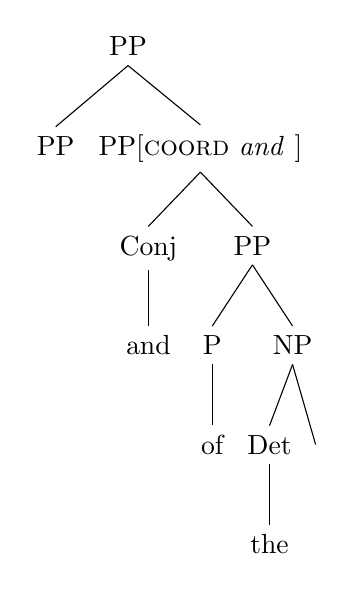
\begin{tikzpicture}
\tikzset{level 1+/.style={level distance=3\baselineskip}}
%\tikzset{frontier/.style={distance from root=23\baselineskip}}
\Tree[.PP
        PP
        [.{PP[\textsc{coord} \emph{and} ]}
          [.Conj and ]
          [.{PP} 
            [.P of ]
            [.NP 
              [.Det the ]
              {\nbar}  ] ] ] 
]
\end{tikzpicture}
\caption{\label{fig-and-of-the}Structure of the fragment \emph{and of the} following
  \citew[\page 32]{PS2001a}}
\end{figure}%
As a result of the interaction of various constraints in a constraint"=based grammar, it emerges that \emph{the}
is part of an NP and this NP is an argument of \emph{of} and furthermore \emph{and} is combined with the relevant
\emph{of}-PP. In symmetric coordination, the first conjunct has the same syntactic properties as the second, which
is why the partial structure of \emph{and of the} allows one to draw conclusions about the category of the conjunct
despite it not being part of the string.

Ewan Klein\aimention{Ewan Klein} noted that Categorial Grammar\indexcg and Minimalist Grammars, which build up more complex
expressions from simpler ones, can sometimes create this kind of fragments \citep[\page 507]{Pullum2013a}.
This is certainly the case for Categorial Grammars with composition rules, which allow one to
combine any sequence of words to form a constituent. If one views derivations as logical proofs, as
is common in some variants of Categorial Grammar, then the actual derivation is irrelevant. What matters is whether a
proof can be found or not. However, if one is interested in the derived structures, then the argument brought forward by Pullum and Scholz is still
valid. For some variants of Categorial Grammar that motivate the combination of constituents based on their prosodic\is{prosody}
and information"=structural properties \citep[Section~3]{Steedman91a}, the problem persists since fragments have
a structure independent of the structure of the entire utterance and independent of their
information"=structural properties within this complete structure. This structure of the fragment
can be such that it is not possible to analyze it with type"=raising rules and composition
rules.

In any case, this argument holds for Minimalist\is{Minimalist Program (MP)} theories since it is not possible to have a combination
of \emph{the} with a nominal constituent if this constituent was not already built up from lexical
material by Merge.

\section{A problem for model"=theoretic approaches?}
\label{Abschnitt-MTS-ten-Hacken}

\mbox{}\Citet[\page 237--238]{TenHacken2007a} discusses the formal assumptions of HPSG\indexhpsg. In HPSG, feature descriptions are used to describe feature
structures. Feature structures must contain all the features belonging to a structure of a certain
type. Additionally, the features have to have a maximally"=specific value (see
Section~\ref{sec-modelle-theorien}). Ten Hacken discusses gender properties\is{gender|(} of the
English noun \emph{cousin}. In English, gender is important in order to ensure the correct binding
of pronouns (see page~\pageref{le-buch} for German): 
\eal
\ex The man$_i$ sleeps. He$_i$ snores.
\ex The woman$_i$ sleeps. He$_{*i}$ snores.
\zl
While \emph{he} in (\mex{0}a) can refer to \emph{man}, \emph{woman} is not a possible antecedent. Ten Hacken's problem is that \emph{cousin}
is not marked with respect to gender. Thus, it is possible to use it to refer to both male and female relatives.
As was explained in the discussion of the case value of \emph{Frau} `woman' in Section~\ref{sec-modelle-theorien}, it is possible for a
value in a description to remain unspecified. Thus, in the relevant feature structures, any
appropriate and maximally specific value is possible. The case of \emph{Frau} can therefore be nominative, genitive, dative or accusative in an actual feature structure.
Similarly, there are two possible genders for \emph{cousin} corresponding to the usages in (\mex{1}).
\eal
\ex I have a cousin$_i$. He$_i$ is very smart.
\ex I have a cousin$_i$. She$_i$ is very smart.
\zl

\noindent
Ten Hacken refers to examples such as (\mex{1}) and claims that these are problematic:
\eal
\ex Niels has two cousins.
\ex How many cousins does Niels have?
\zl
In plural usage, it is not possible to assume that \emph{cousins} is feminine or masculine since the set of relatives can contain
either women or men. It is interesting to note that (\mex{1}a) is possible in English, whereas German is forced to use (\mex{1}b)
to express the same meaning.
\eal
\ex Niels and Odette are cousins.
\ex 
\gll Niels und Odette sind Cousin und Cousine.\\
	 Niels and Odette are cousin.\mas{} and cousin.\fem\\
\zl
Ten Hacken concludes that the gender value has to remain unspecified and this shows, in his opinion, that model"=theoretic analyses
are unsuited to describing language.

If we consider what exactly ten Hacken noticed, then it becomes apparent how one can account for this in a model"=theoretic approach:
Ten Hacken claims that it does not make sense to specify a gender value for the plural form of \emph{cousin}. In a model"=theoretic approach, this can be captured
 in two ways. One can either assume that there are no gender features for referential indices in the
plural, or that one can add a gender value that plural nouns can have.

The first approach is supported by the fact that there are no inflectional differences between the
plural forms of pronouns with regard to gender. There is therefore no reason to distinguish genders
in the plural.
\eal
\ex Niels and Odette are cousins. They are very smart.
\ex The cousins/brothers/sisters are standing over there. They are very smart.
\zl
No distinctions are found in plural when it comes to nominal inflection (\emph{brothers},
\emph{sisters}, \emph{books}). In German, this is different. There are differences with both nominal
inflection and the reference of (some) noun phrases 
with regard to the sexus of the referent.
Examples of this are the previously mentioned examples \emph{Cousin} `male cousin' and
\emph{Cousine} `female cousin' as well as forms with the suffix \suffix{in} as in \emph{Kindergärtnerin} `female nursery teacher'.
However, gender is normally a grammatical notion that has nothing to do with sexus\is{sexus}.
An example is the neuter noun \emph{Mitglied} `member', which can refer to both female and male persons.

The question that one has to ask when discussing Ten Hacken's problem is the following: does gender play a role for pronominal binding
in German? If this is not the case, then the gender feature is only relevant within the morphology
component, and here the gender value is determined for each noun in the lexicon. For the binding of personal pronouns, there is no gender difference in German. 
\ea
\gll Die Schwestern / Brüder / Vereinsmitglieder / Geschwister stehen dort. Sie lächeln.\\
     the sisters.\fem{} {} brothers.\mas{} {} club.members.\neu{} {} siblings stand there they smile.\\
\glt `The sisters/brothers/club members/siblings are standing there. They are smiling.'
\z
Nevertheless, there are adverbials in German that agree in gender with the noun to which they refer \citep[Chapter~6]{Hoehle83}:
\eal
\label{Beispiel-einer-nach-dem-anderen}
\ex
\gll Die Fenster wurden eins nach dem anderen geschlossen.\\
	 the windows.\neu{} were one.\neu{} after the other closed\\
\glt `The windows were closed one after the other.'
\ex 
\gll Die Türen wurden eine nach der anderen geschlossen.\\
	the doors.\fem{} were one.\fem{} after the other closed\\
\glt `The doors were closed one after the other.'
\ex 
\gll Die Riegel wurden einer nach dem anderen zugeschoben.\\
	 the bolts.\mas{} were one.\mas{} after the other closed\\
	 \glt `The bolts were closed one after the other.'
\zl
For animate nouns, it is possible to diverge from the gender of the noun in question and use a form of
the adverbial that corresponds to the biological sex:
\eal
\ex 
\gll Die Mitglieder des Politbüros wurden eines / einer nach dem anderen aus dem Saal getragen.\\
	 the members.\neu{} of.the politburo were one.\neu{} {} one.\mas{} after the other out.of the hall carried\\
\glt `The members of the politburo were carried out of the hall one after the other.'
\ex 
\gll Die Mitglieder des Frauentanzklubs verließen eines / eine nach dem / der anderen im Schutze der Dunkelheit den
Keller.\\
the members.\neu{} of.the women's.dance.club left one.\neu{} {} one.\fem{} after the.\neu{} {} the.\fem{} other in.the protection of.the dark the
basement\\
\glt `The members of the women's dance club left the basement one after the other under cover of darkness.'
\zl
This deviation from gender in favor of sexus can also be seen with binding of personal and relative pronouns with nouns such as
\emph{Weib} `woman' (pej.) and \emph{Mädchen} `girl':
\eal
\ex 
\gll "`Farbe bringt die meiste Knete!"' verriet ein 14jähriges türkisches {\em Mädchen\/}, {\em die\/} die Mauerstückchen am
      Nachmittag am Checkpoint Charlie an Japaner und US-Bürger verkauft.\footnotemark\\
\hspaceThis{"`}color brings the most money revealed a 14-year.old Turkish girl.\neu{} who.\fem{} the wall.pieces
in.the afternoon at Checkpoint Charlie at Japanese and US-citizens sells\\  
\footnotetext{
        taz, 14.06.1990, p.\,6.
      }
\glt `\,``Color gets the most money'' said a 14-year old Turkish girl who sells pieces of the wall to Japanese and American citizens
at Checkpoint Charlie.'
\ex 
\gll Es ist ein junges {\em Mädchen\/}, {\em die\/} auf der Suche nach CDs bei Bolzes reinschaut.\footnotemark\\
	 it is a young girl.\neu{} who.\fem{} on the search for CDs at Bolzes stops.by\\
\footnotetext{
        taz, 13.03.1996, p.\,11.
      }
\glt `It is a young girl looking for CDs that stops by Bolzes.' 
\zl
For examples from Goethe, Kafka and Thomas Mann, see \citew[\page 417--418]{Mueller99a}. 

%\addlines
For inanimate nouns such as those in (\mex{-2}), agreement is obligatory. For the analysis of
German, one therefore does in fact require a gender feature in the plural. In English, this is not
the case since there are no parallel examples with pronouns inflecting for gender. One can therefore
either assume that plural indices do not have a gender feature or that the gender value is
\emph{none}. In the latter case, the feature would have a value and hence fulfill the formal requirements.
(\mex{1}) shows the first solution: plural indices are modeled by feature structures of
type \type{pl-ind} and the \textsc{gender} feature is just not appropriate for such objects.

\ea
\begin{tabular}[t]{@{}l@{~~}l@{\hspace{2cm}}l@{~~}l}
a.& singular index: &
b.& plural index:\\
  &\ms[sg-ind]{
    per & per\\
    num & sg\\
    gen & gender\\
    }
&&\ms[pl-ind]{
    per & per\\
    num & pl\\
    }\vspace{\baselineskip}~
\end{tabular}
\z
The second solution requires the type hierarchy in Figure~\vref{fig-typehierarchy-gender-ten-Hacken} for the subtypes of \type{gender}.
% moved above the figure
With such a type hierarchy \type{none} is a possible value of the \textsc{gen} feature and no
problem will arise.%
\is{gender|)}
\begin{figure}
\begin{forest}
typehierarchy
[ gender
   [fem] [mas] [neu] [none] ]
\end{forest}
\caption{\label{fig-typehierarchy-gender-ten-Hacken}Type hierarchy for one of the solutions of ten Hacken's problem}
\end{figure}%

In general, it is clear that cases such as the one constructed by ten Hacken will never be a problem since there are either
values that make sense, or there are contexts for which there is no value that makes sense and one therefore does not require
the features.

So, while ten Hacken's problem is a non-issue, there are certain problems of a more technical
nature. I have pointed out one such technical problem in \citew[Section~14.4]{Mueller99a}. I show
that spurious ambiguities\is{ambiguity!spurious} arise for a particular analysis of verbal complexes in German when one
resolves the values of a binary feature (\textsc{flip}).  I also show how this problem can be
avoided by the complicated stipulation of a value in certain contexts.%
\is{model"=theoretic grammar|)}


%      <!-- Local IspellDict: en_US-w_accents -->

%% -*- coding:utf-8 -*-

\chapter{The competence/performance distinction}
\label{Abschnitt-Diskussion-Performanz}\label{chap-competence-performance}

The distinction\nocite{VL2006a} between competence and performance\is{competence|(}\is{performance|(}
\citep[Chapter~I.1]{Chomsky65a}, which is assumed by several theories of grammar, was already
discussed in Section~\ref{Abschnitt-Kompetenz-Performanz-TAG} about the analysis of scrambling and
verbal complexes in TAG. Theories of competence are
intended to describe linguistic knowledge and performance theories are assigned the task of
explaining how linguistic knowledge is used as well as why mistakes are made in speech production
and comprehension. A classic example in the competence/""performance discussion are cases of
center self"=embedding\is{self"=embedding}. \citet[\page 286]{CM63a} discuss the following example with
recursively\is{recursion} embedded relative clauses\is{relative clause}: 
\ea
(the rat (the cat (the dog chased) killed) ate the malt)
\z
(\mex{1}b) is a corresponding example in German:
\eal
\ex 
\gll dass der Hund bellt, der die Katze jagt, die die Maus kennt, die im Keller lebt\\
     that the dog.\mas{} barks that.\mas{} the cat chases that.\fem{} the mouse knows who in.the basement lives\\
\glt `that the dog that chases the cat that knows the mouse who is living in the basement is barking'
\ex\label{Bsp-Selbsteinbettung} 
\gll dass er Hund, [$_1$ der die Katze, [$_2$ die die Maus, [$_3$ die im Keller lebt,  $_3$] kennt, $_2$] jagt $_1$] bellt\\
     that the dog {} that the cat {} that the mouse      {}    who in.the basement lives {} knows {} chases {} barks\\
\zl
%
The examples in (\mex{-1}) and (\mex{0}b) are entirely incomprehensible for most people.
If one rearranges the material somewhat, it is possible to process the sentences and assign a
meaning to them.\footnote{
  The sentence in (\mex{0}a) can be continued following the pattern that was used to create the
  sentence. For instance by adding \emph{die unter der
    Treppe lebte, die meine Freunde repariert haben} `who lived under the staircase which my
  friends repaired'. This shows that a restriction of the number of elements that depend on one head
to seven  \citep[\page 322]{Leiss2003a} does not restrict the set of the sentences that are
generated or licensed by a grammar to be finite. There are at most two dependents of each head in
(\mex{0}a). The extraposition of the relative clauses allows the hearer to group material into
processable and reducible chunks, which reduces the cognitive burden during processing.

  This means that the restriction to seven dependents does not cause a finitization of recursion
  (``Ver\-end\-lichung von Rekursivität\is{recursion}'') as was claimed by \citet[\page 322]{Leiss2003a}.
  Leiss argued that Miller could not use his insights regarding short term memory, since he worked
  within Transformational Grammar\is{Transformational Grammar} rather than in \dg. The discussion
  shows that dependency plays an important role, but that linear order is also important for processing.
}
For sentences such as (\mex{0}b), it is often assumed that they fall within our grammatical competence, that is, we possess
the knowledge required to assign a structure to the sentence, although the processing of utterances such as (\mex{0}b) exceeds
language"=independent abilities of our brain.
In order to successfully process (\mex{0}b), we would have to retain the first five noun phrases and corresponding hypotheses
about the further progression of the sentence in our heads and could only begin to combine syntactic material when the verbs appear.
Our brains become overwhelmed by this task. These problems do not arise when analyzing (\mex{0}a) as it is possible
to immediately begin to integrate the noun phrases into a larger unit.

Nevertheless, center self"=embedding of relative clauses can also be constructed in such a way that our brains can handle them. Hans
Uszkoreit\aimention{Hans Uszkoreit} gives the following example:
\ea
\label{Bsp-Selbsteinbettung-Uszkoreit}
\gll Die Bänke, [$_1$ auf denen damals die Alten des Dorfes, [$_2$ die allen Kindern, [$_3$ die vorbeikamen $_3$], freundliche Blicke zuwarfen $_2$], 
lange Stunden schweigend nebeneinander saßen $_1$], mussten im letzten Jahr einem Parkplatz weichen.\\
the benches {} on which back.then the old.people of.the village {} that all children {} that came.by {} friendly glances gave {}
long hours silent next.to.each.other sat {} must in.the last year a car.park give.way.to\\
\glt `The benches on which the older residents of the village, who used to give friendly glances to all the children who came by, used to sit silently next to one 
another for hours had to give way to a car park last year.'
\z
Therefore, one does not wish to include in the description of our grammatical knowledge that
relative clauses are not allowed to be included inside each other as in (\ref{Bsp-Selbsteinbettung})  
as this would also rule out (\ref{Bsp-Selbsteinbettung-Uszkoreit}).

We can easily accept the fact that our brains are not able to process structures past a certain degree of complexity and also that corresponding utterances then become unacceptable.
The contrast in the following examples is far more fascinating:\footnote{
See \citew[\page 227]{GT99a}. \citet[\page 178]{Frazier85a-u} 
attributes the discovery of this kind of sentences to Janet Fodor\aimention{Janet Dean Fodor}.
}
\eal
\ex[\#]{
The patient [ who the nurse [ who the clinic had hired ] admitted ] met Jack.
}
\ex[*]{
The patient who the nurse who the clinic had hired met Jack.
}
\zl
Although (\mex{0}a)  is syntactically well"=formed and (\mex{0}b) is not, \citet{GT99a} were able to
show that (\mex{0}b) is rated better by speakers than (\mex{0}a). It does not occur to some people that an entire
VP is missing\is{Missing VP effect}. There are a number of explanations for this fact, all of which in
some way make the claim that previously heard words are forgotten as soon as new words are heard and
a particular degree of complexity is exceeded (\citealp[\page 178]{Frazier85a-u}; \citealp{GT99a}). 

Instead of developing grammatical theories that treat (\ref{Bsp-Selbsteinbettung}) and (\mex{0}a) as
unacceptable and (\ref{Bsp-Selbsteinbettung-Uszkoreit}) and (\mex{0}b) as acceptable, descriptions
have been developed that equally allow (\ref{Bsp-Selbsteinbettung}),
(\ref{Bsp-Selbsteinbettung-Uszkoreit}), and (\mex{0}a) (competence models) and then additionally
investigate the way utterances are processed in order to find out what kinds of structures our
brains can handle and what kinds of structures it cannot.
The result of this research is then a performance model (see \citew{Gibson98a}, for example).
This does not rule out that there are language"=specific differences affecting language processing.
For example, \citet*{VSLK2010a} have shown that the effects that arise in center self"=embedding structures in German are different from those
that arise in the corresponding English cases such as (\mex{0}):
due to the frequent occurrence of verb"=final structures in German, speakers of German were able to better store predictions about the
anticipated verbs into their working memory (p.\,558).

Theories in the framework of Categorial Grammar\is{Categorial Grammar (CG)},
GB\indexgb, \lfg, \gpsg and \hpsg are theories about our linguistic competence.\footnote{%
  For an approach where the parser is equated with UG, see \citew[Section~3.4]{AC86a}.
  For a performance"=oriented variant of Minimalism, see \citew{Phillips2003a}.

  In Construction Grammar\indexcxg, the question of whether a distinction between competence and
  performance would be justified at all is controversially discussed (see Section~\ref{sec-performance-cxg}).
  \citet*{FSCK99a} also suggest a model -- albeit for different reasons -- where grammatical properties considerably affect
  processing properties. The aforementioned authors work in the framework of Optimality Theory\indexot and show that the OT constraints that
  they assume can explain parsing preferences. OT is not a grammatical theory on its own but rather a meta theory.
  It is assumed that there is a component GEN that creates a set of candidates. A further component EVAL then chooses the most optimal candidate from this set
  of candidates. GEN contains a generative grammar of the kind that we have seen in this book. Normally, a GP/MP variant\indexgb or also LFG\indexlfg is assumed
  as the base grammar. If one assumes a transformational theory, then one automatically has a
  problem with the Derivational Theory of Complexity\is{Derivational Theory of Complexity (DTC)} that
  we will encounter in the following section. If one wishes to develop OT parsing models, then one has to make reference to representational variants of GB
  as the aforementioned authors seem to.%
}
If we want to develop a grammatical theory that directly reflects our cognitive abilities, then there should also be a corresponding performance model to go with
a particular competence model. In the following two sections, I will recount some arguments from \citet{SW2011a} in favor of constraint"=based theories such as
GPSG, LFG and HPSG.

\section{The derivational theory of complexity}
\label{sec-dtc}

The first point discussed by \citet{SW2011a} is the Derivational Theory of Complexity.
In\is{Derivational Theory of Complexity (DTC)|(}\is{transformation|(}  the early days of Transformational Grammar,
it was assumed that transformations were cognitively real, that is, it is possible to measure the consumption of resources
that transformations have.
A sentence that requires more transformations than the analysis of another sentence should therefore also be more difficult for humans
to process. The corresponding theory was dubbed the \emph{Derivational Theory of Complexity} (DTC) and initial experiments
seemed to confirm it \citep{MMK64a,SP65a,CO66a}, so that in 1968 Chomsky still assumed that the
Derivational Theory of Complexity was in fact correct
\citep[\page 249--250]{Chomsky76b-u}.\footnote{%
In the Transformational Grammar literature, transformations were later viewed as a metaphor
(\citealp[\page 170]{Lohnstein2014a}, also in \citealp[Footnote~4]{Chomsky2001a-u}), that is,
it was no longer assumed to have psycholinguistic reality. In \emph{Derivation by phase} and
\emph{On phases}, Chomsky refers once again to processing aspects such as computational and memory load\is{memory} (Chomsky \citeyear[\page 11, 12,
   15]{Chomsky2001a-u}; \citeyear[\page 3, 12]{Chomsky2007a}; \citeyear[\page 138, 145, 146,
   155]{Chomsky2008a}). See also \citew[\page 440]{Marantz2005a} and \citew{Richards2015a}.

  A structure building operation that begins with words and is followed by transformations, as recently assumed by theories in the Minimalist Program,
  is psycholinguistically implausible for sentence parsing. See \citew{Labelle2007a} and Section~\ref{Abschnitt-Inkrementelle-Verarbeitung} for
  more on incremental processing.

  \citet[\page 6]{Chomsky2007a} (written later than \emph{On phases}) seems to adopt a constraint"=based view. He writes that ``a Merge-based system involves parallel operations''
  and compares the analysis of an utterance with a proof and explicitly mentions the competence/performance distinction.
 %
} 
Some years later, however, most psycholinguists rejected the DTC. For discussion of several experiments that testify against
the DTC, see \citew*[\page 320--328]{FBG74a-u}. One set of phenomena where the DTC makes incorrect predictions for respective analyses is that of elliptical\is{ellipsis} constructions, for example
\citep*[\page 324]{FBG74a-u}: in elliptical constructions, particular parts of the utterance are left out or replaced by auxiliaries.
In transformation"=based approaches, it was assumed that (\mex{1}b) is derived from (\mex{1}a) by means of deletion\is{deletion} of
\emph{swims} and (\mex{1}c) is derived from (\mex{1}b) by inserting \emph{do}.
\eal
\ex John swims faster than Bob swims.
\ex John swims faster than Bob.
\ex John swims faster than Bob does.
\zl
The DTC predicts that (\mex{0}b) should require more time to process than (\mex{0}a),
since the analysis of (\mex{0}b) first requires to build up the structure in (\mex{0}a) and then delete \emph{swims}. This prediction was not confirmed.

Similarly, no difference could be identified for the pairs in (\mex{1}) and (\mex{2}) even though one of the sentences, given the relevant theoretical
assumptions, requires more
transformations for the derivation from a base structure \citep*[\page 324]{FBG74a-u}.
\eal
\ex John phoned up the girl.
\ex John phoned the girl up.
\zl
\eal
\ex The bus driver was nervous after the wreck.
\ex The bus driver was fired after the wreck.
\zl
In (\mex{-1}), we are dealing with local reordering of the particle\is{verb!particle} and the object. (\mex{0}b) contains a passive clause that
should be derived from an active clause\is{passive} under Transformational Grammar assumptions. If we compare this sentence with an equally long sentence
with an adjective, like (\mex{0}a), the passive clause should be more difficult to process. This is, however, not the case.

It is necessary to add two qualifications to Sag~\& Wasow's claims: if one has experimental data that show that the DTC makes incorrect predictions for a particular
analysis, this does not necessarily mean that the DTC has been disproved. One could also try to find a different analysis for the phenomenon in question.
For example, instead of a transformation that deletes material, one could assume empty elements for the analysis of elliptical structures that are inserted
directly into the structure without deleting any material (see page~\pageref{np-epsilon} for the
assumption of an empty nominal head in structures with noun ellipsis in German). Data such as (\mex{-2}) would then be irrelevant to the discussion.\footnote{
  \citet[Chapters~1 and ~7]{CJ2005a} argue in favor of analyzing ellipsis as a semantic or pragmatic phenomenon rather than a syntactic
  one anyway.
} 
However, reordering such as (\mex{-1}b) and the passive in (\mex{0}b) are the kinds of phenomena that are typically explained using transformations.

The second qualification pertains to analyses for which there is a representational variant: it is often said that transformations are simply
metaphors (Jackendoff \citeyear[\page
22--23]{Jackendoff2000a}; \citeyear[\page 5, 20]{Jackendoff2007a}): for example, we have seen that extractions with a transformational grammar yield structures that
are similar to those assumed in \hpsg. Figure~\vref{Abbildung-zyklisch-Perkolation} shows cyclic\is{cycle!transformational} movement in \gbt compared
to the corresponding \hpsg analysis.
\begin{figure}
\hfill%
\adjustbox{valign=c}{%
\begin{forest}
[CP
	[NP
		[\_$_ i$]]
	[C$'$
		[C]
		[VP
			[NP]
			[V$'$
				[V]
				[NP
					[\_$_ i$]]]]]]
\end{forest}}
\hfill
\adjustbox{valign=c}{%
\begin{forest}
[CP/NP
	[C]
	[VP/NP
		[NP]
		[V$'$/NP
			[V]
			[NP/NP
				[\_$_ i$]]]]]
\end{forest}}
\hfill\mbox{}%
\caption{Cyclic movement vs.\ feature percolation}\label{Abbildung-zyklisch-Perkolation}
\end{figure}%

In GB, an element is moved to the specifier positions of CP (SpecCP) and can then be moved from there to the next higher SpecCP position.
\eal\settowidth\jamwidth{(HPSG)}
\ex
Chris$_i$, we think [\sub{CP} \_$_i$ Anna claims [\sub{CP} \_$_i$ that David saw \_$_i$]].\jambox{(GB)}
\ex
Chris$_i$, we think [\sub{CP/NP} Anna claims [\sub{CP/NP} that David saw \_$_i$]].\jambox{(HPSG)}
\zl
In HPSG, the same effect is achieved by structure sharing\is{structure sharing}. Information about a long"=distance dependency
is not located in the specifier node but rather in the mother node of the projection itself. In Section~\ref{Abschnitt-Eleminierung-leerer-Elemente},
I will discuss various ways of eliminating empty elements from grammars. If we apply these techniques to structures such as the GB structure
in Figure~\ref{Abbildung-zyklisch-Perkolation}, then we arrive at structures where information about missing elements is integrated into the
mother node (CP) and the position in SpecCP is unfilled. This roughly corresponds to the HPSG structure in Figure~\ref{Abbildung-zyklisch-Perkolation}.\footnote{ 
In Figure~\ref{Abbildung-zyklisch-Perkolation}, additionally the unary branching of C$'$ to CP was omitted in the tree on the right so that C combines directly with VP/NP
to form CP/NP.%
}
It follows from this that there are classes of phenomena that
% \todoandrew{changed `for' to
  % `about'. OK?} 
can be spoken about in terms of transformations without expecting empirical differences with regard to
performance when compared to transformation"=less approaches.
However, it is important to note that we are dealing with an S"=structure in the left"=hand tree in Figure~\ref{Abbildung-zyklisch-Perkolation}. As soon as one assumes
that this is derived by moving constituents out of other structures, this equivalence of approaches disappears.
\is{transformation|)}\is{Derivational Theory of Complexity (DTC)|)}

\section{Incremental processing}
\label{Abschnitt-Inkrementelle-Verarbeitung}

The next important point mentioned by \citet{SW2011a} is the fact that both comprehension and production of language take places incrementally.
As soon as we hear or read even the beginning of a word, we begin to assign meaning and to create structure.
In the same way, we sometimes start talking before we have finished planning the entire utterance.
This is shown by interruptions and self correction in spontaneous speech \citep{CW98a,CFT2002a}.
When it comes to processing spoken speech, \citet{TSKES96a} have shown that we access a word as soon
as we have heard a part of it (see also \citealp{Marslen-Wilson75a}).  The authors of the study carried out an experiment where participants were instructed
to pick up particular objects on a grid and reorganize them. Using eye"=tracking measurements,
Tanenhaus and colleagues could then show that the participants could identify the object in question
earlier if the sound sequence at the beginning of the word was unambiguous than in cases 
where the initial sounds occurred in multiple words. An example for this is a configuration with a candle and candy: \emph{candy} and \emph{candle}
both begin with \emph{can} such that speakers could not yet decide upon hearing this sequence which lexical entry should be accessed. Therefore, there
was a slight delay in accessing the lexical entry when compared to words where the objects in question did not contain the same segment at the
start of the word \citep[\page 1633]{TSKES95a}.

If complex noun phrases were used in the instructions (\emph{Touch the starred yellow
  square}), the participants' gaze fell on the object in question 250ms after it was unambiguously identifiable.
  This means that if there was only a single object with stars on it, then they looked at it after they heard
  \emph{starred}. In cases where there were starred yellow blocks as well as squares, they looked at the square
  only after they had processed the word \emph{square} \citep[\page 1632]{TSKES95a}.
The planning and execution of a gaze lasts 200ms. From this, one can conclude that hearers combine words directly
and as soon as enough information is available, they create sufficient structure in order to capture
the (potential) meaning of an expression and react accordingly.
This finding is incompatible with models that assume that one must have heard a complete noun phrase or even a complete utterance
of even more complexity before it is possible to conclude anything about the meaning of a phrase/utterance. 
In particular, analyses in the Minimalist Program\indexmp which assume that only entire phrases or so"=called phases\is{phase}\footnote{
     Usually, only CP and vP are assumed to be phases.
}
are interpreted (\citew{Chomsky99a} and \citew[\page 441]{Marantz2005a}, who explicitly contrasts the
MP to Categorial Grammar\indexcg) must therefore be rejected as inadequate from a psycholinguistic perspective.\footnote{
% 74
\citet[\page 729--730]{Sternefeld2006a-u} points out that in theories in the Minimalist Program, the common assumption of uninterpretable
features is entirely unjustified. Chomsky assumes that there are features that have to be deleted in the course of a derivation
since they are only relevant for syntax. If they are not checked, the derivation crashes at the interface to semantics.
It follows from this that NPs should not be interpretable under the assumptions of these theories since they contain a number of features
that are irrelevant for the semantics and have to therefore be deleted (see
Section~\ref{sec-features-minimalism} of this book and \citealp{Richards2015a}).
As we have seen, these kinds of theories are incompatible with the facts.
}$^,$\footnote{
  It is sometimes claimed that current Minimalist theories are better suited to explain production (generation)
  than perception (parsing). But these models are as implausible for generation as they are for parsing. The
  reason is that it is assumed that there is a syntax component that generates structures that are
  then shipped to the interfaces. This is not what happens in generation though. Usually speakers
  know what they want to say (at least partly), that is, they start with semantics.
}

With contrastive\is{contrast} emphasis\is{prosody} of individual adjectives in complex noun phrases
(\eg \emph{the BIG blue triangle}), hearers assumed that there must be a corresponding counterpart to the reference object, \eg a small blue triangle.
The eye"=tracking studies carried out by \citet{TSKES96a} have shown that taking this kind of information into account
results in objects being identified more quickly.

Similarly, \citet{ATAF2004a} have shown, also using eye"=tracking studies, that hearers tend to direct their gaze
to previously unmentioned objects if the interlocutor interrupts their speech with \emph{um} or \emph{uh}.
This can be traced back to the assumption that hearers assume that describing previously unmentioned objects is more
complex than referring to objects already under discussion. The speaker can create more time for himself
by using \emph{um}
or \emph{uh}.

Examples such as those above constitute evidence for approaches that assume that when processing language, information from all available
channels is used and that this information is also used as soon as it is available and not only after the structure of the entire utterance or
complete phrase has been constructed.
The results of experimental research therefore show that the hypothesis of a strictly modular\is{modularity} organization
of linguistic knowledge must be rejected.
Proponents of this hypothesis assume that the output of one module constitutes the input of another without a given module having access
to the inner states of another module or the processes taking place inside it.
For example, the morphology module could provide the input for syntax and then this would be
processed later by the semantic module. One kind of evidence for this kind of organization of linguistic knowledge that is often cited
are so"=called \emph{garden path sentences} such as (\mex{1}):
\eal
\ex\label{bsp-horse-past-barn} 
The horse raced past the barn fell.
\ex The boat floated down the river sank.
\zl
The vast majority of English speakers struggle to process these sentences since their parser is led down a garden path
as it builds up a complete structure for (\mex{1}a) or (\mex{1}b) only then to realize that there is another
verb that cannot be integrated into this structure.
\eal
\ex The horse raced past the barn.
\ex The boat floated down the river.
\zl
However, the actual structure of (\mex{-1}) contains a reduced relative clause (\emph{raced past
  the barn} or \emph{floated down the river}). That is the sentences in (\ref{bsp-horse-past-barn})
are semantically equivalent to the sentences in (\mex{1}):
\eal
\ex The horse that was raced past the barn fell.
\ex The boat that was floated down the river sank.
\zl
The failure of the parser in these cases was explained by assuming that syntactic processing
such as constructing a sentence from NP and VP take place independently of the processing of other constraints.
As \citet{CS85a} and others have shown, yet there are data that make this explanation seem less plausible: 
if (\ref{bsp-horse-past-barn}) is uttered in a relevant context, the parser is not misled.
In (\mex{1}), there are multiple horses under discussion and each NP is clearly identified by a relative
clause. The hearer is therefore prepared for a relative clause and can process the reduced relative clause
without being led down the garden path, so to speak.
\ea
The horse that they raced around the track held up fine. The horse that was raced down
    the road faltered a bit. And the horse raced past the barn fell.
\z

\noindent
By exchanging lexical material, it is also possible to modify (\ref{bsp-horse-past-barn}) in such way as to
ensure that processing is unproblematic without having to add additional context. It is necessary
to choose the material so that the interpretation of the noun as the subject of verb in the reduced
relative clause is ruled out. Accordingly, \emph{evidence} in (\mex{1}) refers to an inanimate noun.
It is therefore not a possible agent of \emph{examined}. A hypothesis with \emph{evidence} as the
agent of \emph{examined} is therefore never created when processing this sentence
\citep{SW2011a}.\todostefan{Trueswell, Ferreira and Clifton zitieren \citet{TTG94a,FC86a}}
\ea
The evidence examined by the judge turned out to be unreliable.
\z
Since processing proceeds incrementally, it is sometimes assumed that realistic grammars should be obliged to immediately assign a constituent structure to previously heard
material \citep{AS82a,Hausser92a-u}.
Proponents of this view would assume a structure for the following sentence where every word forms a constituent with the
preceding material:

\ea
\gll {}[[[[[[[[[[[[[[Das britische] Finanzministerium] stellt] dem] angeschlagenen] Bankensystem] des] Landes] mindestens] 200] Milliarden] Pfund] zur] Verfügung].\\
{}\spacebr{}\spacebr{}\spacebr{}\spacebr{}\spacebr{}\spacebr{}\spacebr{}\spacebr{}\spacebr{}\spacebr{}\spacebr{}\spacebr{}\spacebr{}\spacebr{}the British treasury provides the
crippled banking.system of.the country at.least 200 billion pounds to use\\
\glt 'The British Treasury is making at least 200 billion pounds available to the crippled banking system.'
\z
\citet{Pulman85a}, \citet{Stabler91a} and \citet[\page 301--308]{SJ93a} have shown, however, that it is possible to build semantic structures incrementally,
using the kind of phrase structure grammars we encountered in Chapter~\ref{Kapitel-PSG}. This means that a partial semantic representation for the
string \emph{das britische} `the British' can be computed without having to assume that the two words form a constituent in (\mex{0}).
Therefore, one does not necessarily need a grammar that licenses the immediate combination of words directly.
Furthermore, \citew{SJ93a} point out that from a purely technical point of view, synchronous processing is more costly than asynchronous processing since
synchronous processing requires additional mechanisms for synchronization whereas asynchronous processing processes information as soon as it
becomes available (p.\,297--298). Shieber and Johnson do not clarify whether this also applies to synchronous/""asynchronous processing of syntactic and semantic
information. See \citew{SJ93a} for incremental processing and for a comparison of Steedman's Categorial Grammar\indexcg and TAG\indextag.

What kind of conclusions can we draw from the data we have previously discussed? Are there further data that can help to determine the kinds
of properties a theory of grammar should have in order to count as psycholinguistically plausible? \citet*{SWB2003a} and \citet{SW2011a,SW2015a}
list the following properties that a performance"=compatible competence grammar should have:\footnote{
  Also, see \citew{Jackendoff2007a} for reflections on a performance model for a constraint"=based, surface"=oriented linguistic
  theory.
}
\begin{itemize}
\item surface"=oriented
\item model"=theoretic and therefore constraint"=based
\item sign-based organization
\item strictly lexicalist
\item representational underspecification of semantic information
\end{itemize}

\noindent
Approaches such as CG\indexcg, GPSG\indexgpsg, LFG\indexlfg, HPSG\indexhpsg, CxG\indexcxg and TAG\indextag are surface"=oriented
since they do not assume a base structure from which other structures are derived via transformations. Transformational\is{transformation}
approaches, however, require additional assumptions.\footnote{
	An exception among transformational approaches is \citew{Phillips2003a}. Phillips assumes that structures relevant for phenomena such as ellipsis\is{ellipsis},
	coordination\is{coordination} and fronting
	are built up incrementally. These constituents are then reordered in later steps by transformations. For example, in the analysis of (i), the string
	\emph{Wallace saw Gromit in} forms a constituent where \emph{in} is dominated by a node with the label P(P). This node is then turned into a PP
	in a subsequent step (p.\,43--44).
\ea
Wallace saw Gromit in the kitchen.
\z
While this approach is a transformation"=based approach, the kind of transformation here is very idiosyncratic and incompatible with other
variants of the theory. In particular, the modification of constituents contradicts the assumption of Structure Preservation\is{Structure Preservation}
when applying transformations as well as the \emph{No
  Tampering Condition}\is{No Tampering Condition (NTC)} of \citet{Chomsky2008a}. 
Furthermore, the conditions under which an incomplete string such as \emph{Wallace saw Gromit in} forms a constituent are not
entirely clear.
%
} 
This will be briefly illustrated in what follows.
In Section~\ref{Abschnitt-GB-CP-IP-System-Englisch}, we encountered the following analysis of English interrogatives:
\ea
{}[\sub{CP} What$_i$ [\sub{C$'$} will$_k$ [\sub{IP} Ann [\sub{I$'$} \_$_k$ [\sub{VP} read \_$_i$]]]]].
\z
This structure is derived from (\mex{1}a) by two transformations (two applications of \movea):
\eal
\ex[]{
Ann will read what?
}
\ex[*]{
Will Ann read what
}
\zl
The first transformation creates the order in (\mex{0}b) from (\mex{0}a), and the second creates (\mex{-1}) from 
(\mex{0}b).

When a hearer processes the sentence in (\mex{-1}), he begins to build structure as soon as he hears the first word.
Transformations can, however, only be carried out when the entire utterance has been heard.
One can, of course, assume that hearers process surface structures. However, since  -- as we have seen -- they begin to access semantic knowledge
early into an utterance, this begs the question of what we need a deep structure for at all.

In analyses such as those of (\mex{-1}), deep structure is superfluous since the relevant information can be reconstructed
from the traces. Corresponding variants of GB have been proposed in the literature (see page~\pageref{Seite-Representationelle-GB}).
They are compatible with the requirement of being surface"=oriented.
 Chomsky (\citeyear[\page 181]{Chomsky81a}; \citeyear[\page 49]{Chomsky86b}) and
\citet[\page 59--60]{LS92a-u} propose analyses where traces can be deleted. In these analyses,
the deep structure cannot be directly reconstructed from the surface structure and one requires transformations
in order to relate the two.
If we assume that transformations are applied `online' during the analysis of utterances, then this would mean that the
hearer would have to keep a structure derived from previously heard material as well as a list of possible transformations
during processing in his working memory. In constraint"=based grammars, entertaining hypotheses about potential upcoming transformation steps is not
necessary since there is only a single surface structure that is processed directly.
At present, it is still unclear whether it is actually possible to distinguish between these models empirically.
But for Minimalist models with a large number of movements (see Figure~\ref{Abbildung-Remnant-Movement-Satzstruktur}
on page~\pageref{Abbildung-Remnant-Movement-Satzstruktur}, for example), it should be clear that
they are unrealistic since storage space is required to manage the hypotheses regarding such
movements and we know that such short-term memory is very limited in humans.

\citet[\page 27]{FC96a-u} assume that a transformation"=based competence grammar yields a grammar with pre"=compiled
rules or rather templates that is then used for parsing.
Therefore, theorems derived from UG are used for parsing and not axioms of UG directly.
\citet{Johnson89a} also suggests a parsing system that applies constraints from different sub"=theories of GB as early as possible.
This means that while he does assume the levels of representation D"=Structure, S"=Structure, LF and PF, he specifies the relevant
constraints (\xbart, Theta"=Theory\is{theta-Theory@$\theta$-Theory}, Case Theory, \ldots) as logical
conditions that can be reorganized, then be evaluated in a different order, but logically
equivalent, and be used for structure building.%
\footnote{%
\citet[Section~15.7]{Stabler92a-u} also considers a constraint"=based view, but arrives at the conclusion that parsing and other linguistic
tasks should use the structural levels of the competence theory. This would again pose problems for the DTC.%
}
\citet[\page 6]{Chomsky2007a} also compares human parsing to working through a proof, where each step of the proof can be carried out in different
orders. This view does not assume the psychological reality of levels of grammatical representation when processing language, but simply assumes
that principles and structures play a role when it comes to language acquisition\is{acquisition}. 
As we have seen, the question of whether we need UG to explain language acquisition was not yet decided in favor of UG"=based approaches.
Instead, all available evidence seems to point in the opposite direction. However, even if innate linguistic knowledge does exist, the
question arises as to why one would want to represent this as several structures linked via transformations when it is clear that these do not play
a role for humans (especially language learners) when processing language.
Approaches that can represent this knowledge using fewer technical means, \eg without transformations, therefore are preferable.
For more on this point, see \citew[\page 615]{Kuhn2007a}.

The requirement for constraint"=based grammars is supported by incremental processing and also by
the ability to deduce what will follow from previously heard material. \cite{Stabler91a} has pointed
out that Steedman's\aimention{Mark J. Steedman} argumentation with regard to incrementally
processable grammars is incorrect, and instead argues for maintaining a modular view of
grammar. Stabler has developed a constraint"=based grammar where syntactic and semantic
knowledge can be accessed at any time. He formulates both syntactic structures and the semantic
representations attached to them as conjoined constraints and then presents a processing system
that processes structures based on the availability of parts of syntactic and semantic
knowledge. Stabler rejects models of performance that assume that one must first apply all syntactic
constraints before the semantic ones can be applied. If one abandons this strict view of modularity,
then we arrive at something like (\mex{1}):

\ea
(Syn$_1$ $\wedge$ Syn$_2$ $\wedge$ \ldots $\wedge$ Syn$_n$) $\wedge$ (Sem$_1$ $\wedge$ Sem$_2$ $\wedge$ \ldots $\wedge$ Sem$_n$)
\z
Syn$_1$--Syn$_n$ stand for syntactic rules or constraints and Sem$_1$--Sem$_n$ stand for semantic rules or constraints.
If one so desires, the expressions in brackets can be referred to as modules. Since it is possible
to randomly reorder conjoined expressions, one can imagine performance models that first apply some
rules from the syntax module and then, when enough information is present, respective rules from the
semantic module. The order of processing could therefore be as in (\mex{1}), for example: 
\ea
Syn$_2$ $\wedge$ Sem$_1$ $\wedge$ Syn$_1$ $\wedge$ \ldots $\wedge$ Syn$_n$ $\wedge$ Sem$_2$ $\wedge$ \ldots $\wedge$ Sem$_n$
\z

\noindent
If one subscribes to this view of modularity\is{module}, then theories such as HPSG or CxG also have a modular structure.
In the representation assumed in the HPSG variant of \citet{ps} and Sign-Based CxG (see Section~\ref{sec-SbCxG}),
the value of \textsc{syn} would correspond to the syntax module, the value of \textsc{sem} to the semantic module and the value of \textsc{phon}  to the phonology module. If one were to
remove the respective other parts of the lexical entries/dominance schemata, then one would
 be left with the part of the theory corresponding exactly to the level of representation in question.\footnote{
  In current theories in the Minimalist Program, an increasing amount of morphological, syntactic, semantic and 
  information"=structural information is being included in analyses (see Section~\ref{Abschnitt-MP-funktionale-Projektionen}).
  While there are suggestions for using feature"=value pairs \citep[\page 290--291]{SE2002a}, a strict structuring of information
  as in GPSG\indexgpsg, LFG\indexlfg, HPSG\indexhpsg, CxG\indexcxg and variants of
  CG\indexcg and TAG\indextag is not present. This means that there are the levels for syntax, Phonological Form and Logical Form,
  but the information relevant for these levels is an unstructured part of syntax, smeared all over
  syntactic trees.
} 
 \citew{Jackendoff2000a} argues for this form of modularity with the relevant interfaces between the modules for phonology, syntax, semantics and further modules from other areas of cognition. 
Exactly what there is to be gained from assuming these modules and how these could be proved empirically remains somewhat unclear to me. For skepticism with regard to the very concept of modules, see
\citew[\page 22,27]{Jackendoff2000a}. For more on interfaces and modularization in theories such as LFG\indexlfg and HPSG\indexhpsg, see \citew{Kuhn2007a}.

Furthermore, \citet[\page 53--54]{SW2015a} argue that listeners often leave semantic
interpretation underspecified until enough information is present either in the utterance itself or
 the context. They do not commit to a certain reading early and run into garden paths or backtrack
to other readings. This is modeled appropriately by theories that use a variant of underspecified
semantics. For a concrete example of underspecification in semantics see Section~\ref{sec-MRS-wieder}.

In conclusion, we can say that surface"=oriented, model"=theoretic and strongly lexicalist
grammatical theories such as CG, LFG, GPSG, HPSG, CxG and the corresponding GB/MP variants (paired with appropriate semantic representations) can plausibly be combined with processing
models, while this is not the case for the overwhelming majority of GB/MP theories.
\is{competence|)}\is{performance|)}


%      <!-- Local IspellDict: en_US-w_accents -->

%% -*- coding:utf-8 -*-
\chapter{Language acquisition}
\label{chap-acquisition}

Linguists\is{acquisition|(} and philosophers are fascinated by the human ability to acquire language. Assuming the relevant input during childhood,
language acquisition normally takes place completely effortlessly.
\citet[\page  24--25]{Chomsky65a} put forward the requirement that a grammatical theory must provide a plausible model of language acquisition.
Only then could it actually explain anything and would otherwise remain descriptive at best. In this section, we will discuss
theories of acquisition from a number of theoretical standpoints.


\section{Principles \& Parameters}
\label{Abschnitt-PP}\label{sec-pro-drop}

A\is{parameter|(}\is{Principles \& Parameters|(} very influential explanation of language acquisition is Chomsky's Principles \& Parameters model
\citeyearpar{Chomsky81a}. Chomsky assumes that there is an innate Universal Grammar that contains knowledge that is equally relevant for all languages.
Languages can then vary in particular ways. For every difference between languages in the area of core grammar\is{core grammar}, there is a feature with a specific
value. Normally, the value of a parameter is binary, that is, the value is either `+' or `$-$'.
Depending on the setting of a parameter, a language will have certain properties, that is, setting a parameter determines whether
a language belongs to a particular class of languages.
Parameters are assumed to influence multiple properties of a grammar simultaneously \citep[\page 6]{Chomsky81a}. For example, \citet{Rizzi86a} claims
that the pro"=drop parameter\is{parameter!pro"=drop} affects whether referential subjects can be omitted, the absence of expletives, subject
extraction\is{extraction!subject} from clauses with complementizers (\emph{that}-t contexts\is{that-t}) and interrogatives and
finally the possibility of realizing the subject postverbally in VO"=languages (see
\citealp[Section~4.3]{Chomsky81a}; \citealp[\page 12]{Meisel95a}). It has been noted that there are counter"=examples to all the correlations assumed.\footnote{%
\label{fn-Expletiva-Pro-Drop}%
  See \citew{Haider94c-u} and \citew[Section~2.2]{Haider2001a} for an overview. Haider assumes that there is at least a correlation
  between the absence of expletive subjects and pro"=drop. However, Galician\il{Galician} is a pro"=drop language with expletive subject
  pronouns \citep[Section~2.5]{RU90a-u}. \citet[\page 314]{Franks95a-u} cites Upper\il{Sorbian!Upper} and Lower Sorbian\il{Sorbian!Lower} as pro"=drop
  languages with expletive subjects. \citet[\page 218]{SP2002b} point out that there is an expletive pronoun \emph{ci} in modern Italian\il{Italian}
  although Italian\il{Italian} is classed as a pro"=drop language.}
Another example of a parameter is the Head Directionality Parameter discussed in Section~\ref{Abschnitt-Kopfstellungsparameter}.
As was shown, there are languages where heads govern in different directions. In his overview article, \citet{Haider2001a} still mentions
the parametrized Subjacency Principle\is{parameter!subjacency} but notes that subjacency\is{subjacency} is no longer assumed as a principle
in newer versions of the theory (see Section~\ref{Abschnitt-Subjazenz-Extraktion} for more on subjacency).

\citet{Snyder2001a} discovered a correlation of various phenomena with productive root compounding
as it is manifested for instance in compounding of two nouns. He argues that the acquisition of
complex predicate formation is connected to the acquisition of compound structures and that there is
a parameter that is responsible for this type of compounding and simultaneously for the following set of
phenomena:
\eal\settowidth\jamwidth{(double-object dative)}
\ex John painted the house red.                 \jambox{(resultative\is{resultative construction})}
\ex Mary picked the book up/picked up the book. \jambox{(verb-particle\is{verb!particle})}
\ex Fred made Jeff leave.                       \jambox{(\emph{make}-causative)}
\ex Fred saw Jeff leave.                        \jambox{(perceptual report)}
\ex Bob put the book on the table.              \jambox{(\emph{put}-locative)}
\ex Alice sent the letter to Sue.               \jambox{(\emph{to}-dative)}
\ex Alice sent Sue the letter.                  \jambox{(double-object dative\is{verb!ditransitive})}
\zl 
Snyder examined languages from various language groups: Afroasiatic, Austroasiatic, Austronesian,
Finno-Ugric, Indo-European (Germanic, Romance, Slavic), Japanese"=Korean, Niger"=Kordofanian (Bantu),
and Sino"=Tibetan, as well as American Sign\il{sign language!American (ASL)} Language and the language isolate Basque\il{Basque}. The languages
that were examined either had all of these phenomena or none. This was tested with native speakers
of the respective languages. In addition the claim that these phenomena are acquired once noun-noun
compounds are used productively was tested for English using CHILDES data. The result was positive
with the exception of the double object construction, for which an explanation was provided. The
correlation of the phenomena in (\mex{0}) is interesting and was interpreted as proof of the
existence of a parameter that correlates several phenomena in a language. However, \citet{Son2007a}
and \citet{SonS2008a} showed that Snyder's claims for Japanese\il{Japanese} were wrong and that there
are further languages like Korean\il{Korean}, Hebrew\il{Hebrew}, Czech\il{Czech},
Malayalam\il{Malayalam}, Javanese\il{Javanese}  in which some of the phenomena show no correlations. 
%% \citet[\page 395]{SonS2008a} conclude that language"=wide parameters of the type
%% discussed here do never partition the world languages into two sets and that all parameters that
%% were suggested in the past had to be subdivided into smaller ones. They therefore suggest that parametric variation
%% is confined to lexical items.

%\addlines[2]
\largerpage[2]
\citet{GW94a} discuss the acquisition of constituent order and assume three parameters that concern the
position of the verb relative to the subject (SV vs.\ VS)\is{parameter!SV} and relative to the
object (VO vs.\ OV)\is{parameter!V2} as well as the V2"=property\is{parameter!V2}. There is no consensus in the literature about which
parameters determine the make-up of languages (see \citealp[Section~3.2]{Newmeyer2005a} and \citealp{Haspelmath2008a}
for an overview and critical discussion).
\citet[\page 346--347]{Fodor98a} assumes that there are 20 to 30 parameters, \citet[\page 408]{GW94a}
mention the number 40, \citet[\page 349]{Baker2003b} talks of 10 to 20 and \citet[\page 541]{RH2005a}
of 50 to 100. There is no consensus in the literature as to which parameters one should assume, how they interact
and what they predict. However, it is nevertheless possible to contemplate how a grammar of an individual language
could be derived from a UG with parameters that need to be set.
Chomsky's original idea \citeyearpar[Section~3.5.1]{Chomsky86} was that the child sets the value of
a parameter based on the language input as soon as the relevant evidence is present from the input
(see also \citealp*{GW94a,NKN2001a}). At a given point in time, the learner has a grammar with certain parameter
 settings that correspond to the input seen so far. In order to fully acquire a grammar, all parameters must be assigned a value. In theory,
 thirty utterances should be enough to acquire a grammar with thirty parameters if these utterances
 provide unambiguous evidence for a particular parameter value.

This approach has often been criticized. If setting a parameter leads to a learner using a
different grammar, one would expect sudden changes in linguistic behavior. This is, however,
not the case (\citealp[\page 731]{Bloom93a}). \citet[\page 343--344]{Fodor98a} also notes
the following three problems: 1) Parameters can affect things that are not visible from the
perceptible constituent order. 2) Many sentences are ambiguous with regard to the setting of a particular
parameter, that is, there are sometimes multiple combinations of parameters compatible with one
utterance. Therefore, the respective utterances cannot be used to set any parameters \citep{BN96a,Fodor98b}. 3) There is a problem with the interaction of parameters.
Normally multiple parameters play a role in an utterance such that it can be difficult to determine
which parameter contributes what and thus how the values should be determined.\nocite{Pullum83a}

Points 1) and 2) can be explained using the constituent order parameters of Gibson \& Wexler:\il{English}
imagine a child hears sentences such as the English and the German example in (\mex{1}):
\eal
\ex Daddy drinks juice.
\ex 
\gll Papa trinkt Saft.\\
     daddy drinks juice\\
\zl
These sentences look exactly the same, even though radically different structures are assumed for each.
According to the theories under discussion, the English sentence has the structure shown in Figure~\ref{Abb-GB-englischer-Satz-ohne-Hilfsverb} on
page~\pageref{Abb-GB-englischer-Satz-ohne-Hilfsverb} given in abbreviated form in (\mex{1}a).
The German sentence, on the other hand, has the structure in Figure~\ref{Abb-GB-Vorfeldbesetzung} 
on page~\pageref{Abb-GB-Vorfeldbesetzung} corresponding to (\mex{1}b):
\eal
\ex {}[\sub{IP} [Daddy [\sub{I$'$} \_$_k$ [\sub{VP} drinks$_k$ juice]]].
\ex {}[\sub{CP} Papa$_i$ [\sub{C$'$} trinkt$_k$ [\sub{IP} \_$_i$ [\sub{I$'$} [\sub{VP} Saft \_$_k$] \_$_k$]]]].
\zl
English has the basic constituent order SVO\is{SVO}. The verb forms a constituent with the object (VP) and this
is combined with the subject. The parameter setting must therefore be SV, VO and $-$V2. German,
on the other had, is analyzed as a verb"=final and verb"=second language and the parameter values
would therefore have to be SV, OV and $+$V2. If we consider the sentences in (\mex{-1}), we see that
both sentences do not differ from one another with regard to the order of the verb and its arguments.

\citet{Fodor98a,Fodor98b} concludes from this that one first has to build a structure in order to see
what grammatical class the grammar licensing the structure belongs to since one first needs the structure
in (\mex{0}b) in order to be able to see
that the verb in the partial constituent occurs after its argument in the VP (Saft \_$_k$). The question is now how one achieves
this structure. A UG with 30 parameters corresponds to 2$^{30}$ = 1,073,741,824 fully instantiated grammars.
It is an unrealistic assumption that children try out these grammars successively or simultaneously.

\largerpage[2]
\citet{GW94a} discuss a number of solutions for this problem: parameters have a default value\is{parameter!default value}
and the learner can only change a parameter value if a sentence that could previously not be analyzed
can then be analyzed with the new parameter setting (\emph{Greediness Constraint}\is{Greediness Constraint}).
In this kind of procedure, only one parameter can be changed at a time
(\emph{Single Value Constraint}\is{Single Value Constraint}),
which aims at ruling out great leaps leading to extremely different grammars (see \citealp[\page 612--613]{BN96a}, however).
This reduces the processing demands, however with 40 parameters, the worst case could still be that
one has to test 40 parameter values separately, that is, try to parse a sentence with 40 different
grammars. This processing feat is still unrealistic, which is why \citet[\page 442]{GW94a} additionally
assume that one hypothesis is tested per input sentence.
A further modification of the model is the assumption that certain parameters only begin to play a role
during the maturation\is{maturation} of the child. At a given point in time, there could be only a few accessible parameters
that also need to be set. After setting these parameters, new parameters could become available.

In their article, Gibson \& Wexler show that the interaction between input and parameter setting is in no way trivial.
In their example scenario with three parameters, a situation can arise in which a learner sets a parameter in order to analyze
a new sentence, however setting this parameter leads to the fact that the target grammar cannot be acquired because only one value can
be changed at a time and changes can only be made if more sentences can be analyzed than before. The learner reaches a so"=called
local maximum\is{local maximum} in these problematic cases.\footnote{%
	If one imagines the acquisition process as climbing a hill, then the Greediness Constraint\is{Greediness Constraint} ensures
	that one can only go uphill. It could be the case, however, that one begins to climb the wrong hill and can no longer get back down.}
Gibson \& Wexler then suggest assigning a default value to particular parameters, whereby the default value is the one that will cause the learner
to avoid problematic situations. For the V2 parameter\is{parameter!V2}, they assume `$-$' as the default value\is{parameter!default value}.

%\addlines[2]
\citet{BN96a} show that Gibson \& Wexler calculated the problematic conditions incorrectly and
that, if one shares their assumptions, it is even more frequently possible
to arrive at parameter combinations from which it is not possible to reach the target grammar by changing individual parameter values.
They show that one of the problematic cases not addressed by Gibson \& Wexler is $-$V2 (p.\,609) and that the assumption of a default value
for a parameter does not solve the problem as both `+' and `--' can lead to problematic combinations of parameters.\footnote{
  \citet{Kohl99a,Kohl2000a} has investigated this acquisition model in a case with twelve parameters. Of the 4096 possible grammars,
  2336 (57\%) are unlearnable if one assumes the best initial values for the parameters.
}
In their article, Berwick and Niyogi show that learners in the example scenario above (with three
parameters) learn the target grammar faster if one abandons the Greediness\is{Greediness Constraint} 
or else the Single Value Constraint\is{Single Value Constraint}.
They suggest a process that simply randomly changes one parameter if a sentence cannot be analyzed (\emph{Random Step}\is{Random Step}, p.\,615--616).
The authors note that this approach does not share the problems with the local maxima \is{local maximum} that Gibson \& Wexler had in their example and that it also reaches its goal faster
than theirs. However, the fact that \emph{Random Step} converges more quickly has to do with the quality of the parameter space (p.\,618).
Since there is no consensus about parameters in the literature, it is not possible to assess how the entire system works.

\citet[\page 453]{Yang2004a} has criticized the classic Principles \& Parameters model since abrupt switching between grammars after setting
a parameter cannot be observed. Instead, he proposes the following learning mechanism:
\ea
For an input sentence, $s$, the child:
(i) with probability P$_i$ selects a grammar G$_i$, (ii) analyzes $s$ with G$_i$, (iii) if successful, reward G$_i$ by increasing P$_i$,
otherwise punish G$_i$ by decreasing P$_i$.
\z
Yang discusses the example of the pro"=drop\is{parameter!pro"=drop|(} and topic drop parameters\is{parameter!topic drop}. In pro"=drop languages (\eg Italian\il{Italian|}),
it is possible to omit the subject and in topic drop languages (\eg Mandarin Chinese\il{Mandarin Chinese}), it possible to omit both the subject and the object if it is
a topic. Yang compares English-speaking\il{English|(} and Chinese-speaking\il{Mandarin Chinese} children noting that English children omit both subjects and objects
in an early linguistic stage. He claims that the reason for this is that English-speaking children start off using the Chinese grammar.

The pro"=drop parameter is one of the most widely discussed parameters in the context of Principles \& Parameters theory and it will
therefore be discussed in more detail here. It is assumed that speakers of English have to learn that all sentences in English require
a subject, whereas speakers of Italian learn that subjects can be omitted.
One can observe that children learning both English\il{English} and Italian\il{Italian} omit subjects (German children too in fact).
Objects are also omitted notably more often than subjects.
There are two possible explanations for this: a competence"=based\is{competence} one and a performance"=based\is{performance} one.
In competence"=based approaches, it is assumed that children use a grammar that allows them to omit subjects and then only later acquire
the correct grammar (by setting parameters or increasing the rule apparatus). In performance"=based approaches, by contrast, the omission of subjects
is traced back to the fact that children are not yet capable of planning and producing long utterances due to their limited brain capacity.
Since the cognitive demands are greatest at the beginning of an utterance, this leads to subjects beings increasingly left out.
 \citet{Valian91a} investigated these various hypotheses and showed that the frequency with which children learning English and Italian respectively omit subjects
 is not the same. Subjects are omitted more often than objects. She therefore concludes that competence"=based explanations are
 not empirically adequate.\todostefan{hier fehlt irgendwie was bei den Details} The omission of
 subjects should then be viewed more as a performance phenomenon (see also \citealp{Bloom93a}). 
 Another argument for the influence of performance factors is the fact that articles of subjects are
 left out more often than articles of objects (31\% vs.\ 18\%, see \citealp[\page
   440]{Gerken91a}). As Bloom notes, no subject article"=drop parameter has been proposed so
 far\is{parameter!subject article drop}. If we explain this phenomenon as a performance phenomenon, then it is also plausible to assume that
the omittance of complete subjects is due to performance issues.\il{Italian|)}\il{English|)}

\citet{Gerken91a} shows that the metrical properties of utterances also play a role: in experiments where children had to repeat sentences,
they omitted the subject/article of the subject more often  than the object/article of the object. Here, it made a difference whether the intonation pattern
was iambic\is{iambus} (weak-strong) or trochaic\is{trochee} (strong-weak). It can even be observed with individual words that children leave out
weak syllables at the beginning of words more often than at the end of the word. Thus, it is more probable that ``giRAFFE'' is reduced to ``RAFFE'' than
``MONkey'' to ``MON''. Gerken assumes the following for the metrical\is{metrics} structure of utterances:
\begin{enumerate}
\item A metrical foot contains one and only one strong syllable.
\item Create maximally binary left-to-right feet.
\item Metrical structure is independent of syntactic structure.
\end{enumerate}
Subject pronouns in English are sentence"=initial and form a iambic foot with the following strongly emphasized verb as in (\mex{1}a).
Object pronouns, however, can form the weak syllable of a trochaic foot as in (\mex{1}b). 
\eal
\ex she KISSED $+$ the DOG
\ex the DOG $+$ KISSED her
\ex PETE $+$ KISSED the $+$ DOG
\zl
Furthermore, articles in iambic feet as in the object of (\mex{0}a) and the subject of (\mex{0}b) are omitted more often
than in trochaic feet such as with the object of (\mex{0}c).

It follows from this that there are multiple factors that influence the omission of elements and that one cannot simply take the behavior
of children as evidence for switching between two grammars.

Apart from what has been discussed so far, the pro"=drop parameter is of interest for another reason: there is a problem when it comes to setting parameters. The standard explanation is
that learners identify that a subject must occur in all English sentences, which is suggested by the appearance of expletive pronouns\is{pronoun!expletive} in 
the input.

As discussed on page~\pageref{fn-Expletiva-Pro-Drop}, there is no relation between the pro"=drop property and the presence of expletives
in a language. Since the pro"=drop property does not correlate with any of the other putative properties either, only the existence
of subject"=less sentences in the input constitutes decisive evidence for setting a parameter. The problem is that there are grammatical utterances
where there is no visible subject. Examples of this are imperatives such as (\mex{1}), declaratives
with a dropped subject as in (\mex{2}a) and even declarative sentences without an expletive such as the  
example in (\mex{2}b) found by \citet[\page 32]{Valian91a} in the New York Times.
\eal
\label{Beispiel-Imperativ-Englisch}
\ex Give me the teddy bear!
\ex Show me your toy!
\zl
\eal
\ex She'll be a big hit. Sings like a dream.\label{ex-sings-like-a-dream}
\ex Seems like she always has something twin-related perking.
\zl
The following title of a Nirvana\is{Nirvana} song also comes from the same year as Valian's article:
\ea
Smells like Teen Spirit.\\
\z
Teen Spirit refers to a deodorant and \emph{smell} is a verb that, both in German and English, requires a referential subject but can also be used with an expletive \emph{it} as subject.
The usage that Kurt Cobain had in mind cannot be reconstructed\footnote{
  See \url{http://de.wikipedia.org/wiki/Smells_Like_Teen_Spirit}. 18.04.2010.
}, independent of the intended meaning, however, the subject in (\mex{0}) is missing.
Imperatives do occur in the input children have and are therefore relevant for acquisition.
\citet[\page 33]{Valian91a} says the following about them:
\begin{quote}
What is acceptable in the adult community forms part of the child's input, and
is also part of what children must master. The utterances that I have termed
``acceptable'' are not grammatical in English (since English does not have pro
subjects, and also cannot be characterized as a simple VP). They lack subjects
and therefore violate the extended projection principle\is{Extended Projection Principle (EPP)} \citep{Chomsky81a}, which we are assuming.

   Children are exposed to fully grammatical utterances without subjects, in the
form of imperatives. They are also exposed to acceptable utterances which are
not fully grammatical, such as [(\ref{ex-sings-like-a-dream})], as well as forms like, ``Want lunch now?'' The
American child must grow into an adult who not only knows that overt subjects
are grammatically required, but also knows when subjects can acceptably be
omitted. The child must not only acquire the correct grammar, but also master
the discourse conditions that allow relaxation of the grammar. \citep[\page 33]{Valian91a}
\end{quote}
This passage turns the relations on their head: we cannot conclude from the fact that a particular grammatical
theory is not compatible with certain data, 
that these data should not be described by this theory, instead we should modify the incompatible
grammar or, if this is not possible, we should reject it.
Since utterances with imperatives are entirely regular, there is no reason to categorize them as utterances that
do not follow grammatical rules. The quotation above represents a situation where a learner has to acquire two
grammars: one that corresponds to the innate grammar and a second that partially suppresses the rules of innate grammar
and also adds some additional rules.

The question we can pose at this point is: how does a child distinguish which of the data it hears are relevant for which of the two grammars?
\is{parameter!pro"=drop|)}

\citet[\page 347]{Fodor98a} pursues a different analysis that does not suffer from many of the aforementioned problems.
 Rather than assuming that learners try to find a correct grammar among a billion others, she instead assumes that
 children work with a single grammar that contains all possibilities.
She suggests using parts of trees (\emph{treelets}) rather than parameters. These treelets can also be underspecified and
in extreme cases, a treelet can consist of a single feature \citep[\page 6]{Fodor98b}.
A language learner can deduce whether a language has a given property from the usage of a particular treelet.
As an example, she provides a VP treelet consisting of a verb and a prepositional phrase. 
This treelet must be used for the analysis of the VP occurring in \emph{Look at the
  frog}. Similarly, the analysis of an interrogative clause with a fronted \emph{who} would make use
of a treelet with a \emph{wh}"=NP in the specifier of a complementizer phrase (see Figure~\ref{Abb-GB-Wh} on page~\pageref{Abb-GB-Wh}).
In Fodor's version of \ppt, this treelet would be the parameter that licenses \emph{wh}"=movement in (overt) syntax.
Fodor assumes that there are defaults\is{parameter!default value} that allow a learner to parse a sentence even when no or very few
parameters have been set. This allows one to learn from utterances that one would have not otherwise been able to use since there would have
been multiple possible analyses for them. Assuming a default can lead to misanalyses, however: due to a default value, a second
parameter could be set because an utterance was analyzed with a treelet t$_1$ and t$_3$, for example, but t$_1$ was not suited to the particular
language in question and the utterance should have instead been analyzed with the non"=default treelet t$_2$ and the treelet t$_{17}$.
In this acquisition model, there must therefore be the possibility to correct wrong decisions in the parameter setting process. 
Fodor therefore assumes that there is a frequency"=based degree of activation for parameters (p.\,365): treelets that are often
used in analyses have a high degree of activation, whereas those used less often have a lower degree of activation.
In this way, it is not necessary to assume a particular parameter value while excluding others.

Furthermore, Fodor proposes that parameters should be structured hierarchically, that is, only if a parameter has a particular value
does it then make sense to think about specific other parameter values.

Fodor's analysis is -- as she herself notes \citep[\page 385]{Fodor2001a} -- compatible with theories such as HPSG\indexhpsg and TAG\indextag.
\citet[\page 147]{ps} characterize UG as the conjunction of all universally applicable principles:
\ea
UG = P$_1$ $\wedge$ P$_2$ $\wedge$ \ldots{} $\wedge$ P$_n$
\z
As well as principles that hold universally, there are other principles that are specific to a particular language
or a class of languages. Pollard \& Sag give the example of the constituent ordering principle that only holds for English.
English\il{English} can be characterized as follows if one assumes that P$_{n + 1}$--P$_m$ are language"=specific principles,  
L$_{1}$--L$_p$ a complete list of lexical entries and R$_{1}$--R$_q$ a list of dominance schemata relevant for English.
\ea
English = P$_1$ $\wedge$ P$_2$ $\wedge$ \ldots{} $\wedge$ P$_m$ $\wedge$ (L$_{1}$ $\vee$ \ldots{}
$\vee$ L$_p$ $\vee$ R$_{1}$ $\vee$ \ldots{} $\vee$  R$_q$)
\z
In Pollard \& Sag's conception, only those properties of language that equally hold for all languages are
part of UG. Pollard \& Sag do not count the dominance schemata as part of this. However, one can indeed also describe
UG as follows:
\ea
%UG = P$_1$ $\wedge$ P$_2$ $\wedge$ \ldots{} $\wedge$ P$_n$ $\wedge$ (R$_{en\mbox{-}1}$ $\vee$ \ldots{} $\vee$
%R$_{en\mbox{-}q}$  $\vee$ R$_{de\mbox{-}1}$ $\vee$ \ldots{} $\vee$ R$_{de\mbox{-}r}$ $\vee$ \ldots )
$
\mathrm{UG} = 
  \mathrm{P}_1 
  \wedge 
  \mathrm{P}_2 
  \wedge 
  \ldots 
  \wedge 
  \mathrm{P}_n 
  \wedge
              (\mathrm{R}_{\mathrm{en}\mathdash1} 
              \vee 
              \ldots 
              \vee 
              \mathrm{R}_{\mathrm{en}\mathdash q} 
              \vee  
              \mathrm{R}_{\mathrm{de}\mathdash1} 
              \vee 
              \ldots 
              \vee 
              \mathrm{R}_{\mathrm{de}\mathdash r}
	      \vee 
	      \ldots)
$
\z
%\addlines
\largerpage
P$_1$--P$_n$ are, as before, universally applicable principles and
$\mathrm{R}_{\mathrm{en}\mathdash1}$--$\mathrm{R}_{\mathrm{en}\mathdash q}$ are the
(core) dominance schemata of English and $\mathrm{R}_{\mathrm{de}\mathdash1}$--$\mathrm{R}_{\mathrm{de}\mathdash r}$ are the dominance schemata in
German. The dominance schemata in (\mex{0}) are combined by means of disjunctions, that is, not every disjunct needs to have a realization in a specific language. Principles can make reference
to particular properties of lexical entries and rule out certain phrasal configurations.
If a language only contains heads that are marked for final"=position in the lexicon, then grammatical rules that
require a head in initial position as their daughter can never be combined with these heads or their projections.
Furthermore, theories with a type system are compatible with Fodor's approach to language acquisition because 
constraints can easily be underspecified. As such, constraints in UG do not have to make reference to all properties
of grammatical rules: principles can refer to feature values, the language"=specific values themselves do not have to
already be contained in UG. Similarly, a supertype describing multiple dominance schemata that have
similar but language"=specific instantiations can also be part of UG, however the language"=specific details remain open and are then deduced by the learner
upon parsing (see \citealp[Section~9.2]{AW98a}). The differences in activation assumed by Fodor can be captured
by weighting the constraints: the dominance schemata $\mathrm{R}_{\mathrm{en}\mathdash1}$--$\mathrm{R}_{\mathrm{en}\mathdash q}$ etc.\ are sets of
feature"=value pairs as well as path equations. As explained in Chapter~\ref{Abschnitt-Diskussion-Performanz}, 
weights can be added to such constraints and also to sets of constraints. In Fodor's acquisition model, given a German input, the weights for the rules
of English would be reduced and those for the German rules would be increased. Note that in Pollard
\& Sag's acquisition scenario, there are no triggers\is{trigger} for parameter
setting unlike in Fodor's model.
Furthermore, properties that were previously disjunctively specified as part of UG will now be
acquired directly. Using the treelet t$_{17}$ (or rather a possibly underspecified dominance
schema), it is not the case that the value `+' is set for a parameter P$_5$  but rather the activation
potential of t$_{17}$ is increased such that t$_{17}$ will be prioritized for future
analyses.
\is{parameter|)}\is{Principles \& Parameters|)}


\section{Principles and the lexicon}

A variant of the UG"=driven theory of language acquisition would be to assume that principles are so general that they hold
for all languages and individual languages simply differ with regard to their lexicon.
Principles then refer to properties of combined entities. Parameters therefore migrate from principles into the lexicon
\citep[\page 2]{Chomsky99a}. See \citet{MR2010a} for a study of Romance languages in this model and
\citet[\page 395]{SonS2008a} for an analysis of Snyder's examples that were discussed in the
previous subsection.

At this point, one can observe an interesting convergence in these approaches: most of the theories discussed here assume a very
general structure for the combination of heads with their arguments. For example, in Categorial Grammar and the Minimalist Program,
these are always binary functor"=argument combinations. The way in which constituents can be ordered in a particular language depends
on the lexical properties of the combined elements.

The question that is being discussed controversially at present is whether the spectrum of lexical properties is determined by UG 
\citep[\page 6--7]{Chomsky2007a} and whether all areas of the language can be described with the same general combinatorial possibilities (see Section~\ref{Abschnitt-Phrasale-Konstruktionen} on phrasal constructions).

In Section~\ref{Abschnitt-PP}, I have shown what theories of acquisition assuming innate language
specific knowledge can look like and also that variants of such acquisition theories are compatible
with all the theories of grammar we have discussed.  During this discussion, one should bear in
 mind the question of whether it makes sense at all to assume that English children
use parts of a Chinese grammar during some stages of their acquisition process (as suggested by
\citealp[\page 453]{Yang2004a}), or whether the relevant phenomena can be explained in different ways.
In the following, I will present some alternative approaches that do not presuppose innate language
specific knowledge, but instead assume that language can simply be acquired from the input. The
following section will deal with pattern"=based approaches and
Section~\ref{Abschnitt-Selektionsbasierter-Spracherwerb} will discuss the lexically"=oriented variant
of input"=based language acquisition.

\section{Pattern"=based approaches}
\label{Abschnitt-musterbasiert}

\largerpage
\mbox{}\citet[\page 7--8]{Chomsky81a} proposed that languages can be divided into a core
area\is{core grammar} and a periphery\is{periphery}. The core contains all regular aspects of
language. The core grammar of a language is seen as an instantiation of UG. Idioms\is{idiom} and
other irregular parts of language are then part of the periphery.  Critics of the Principles \&
Parameters model have pointed out that idiomatic and irregular constructions constitute a relatively
large part of our language and that the distinction, both fluid and somewhat arbitrary, is only
motivated theory"=internally (\citealp[Chapter~7]{Jackendoff97a}; \citealp{Culicover99a-u};
\citealp[\page 5]{GSag2000a-u}; \citealp[\page 48]{Newmeyer2005a}; \citealp[\page 619]{Kuhn2007a}).
For example, it is possible to note that there are interactions between various idioms and syntax
\citep*{NSW94a}.  Most idioms in German with a verbal component allow the verb to be moved to
initial position (\mex{1}b), some allow that parts of idioms can be fronted (\mex{1}c) and some can
undergo passivization (\mex{1}d).

\addlines
\eal
\ex 
\gll dass er ihm den Garaus macht\\
	 that he him the \textsc{garaus} makes\\
\glt `that he finishes him off (kills him)'
\ex 
\gll Er macht ihm den Garaus.\\
	 he makes him the \textsc{garaus}\\
\glt `He finishes him off.'
\ex
In Amerika sagte man der Kamera nach, die größte Kleinbildkamera der Welt zu sein. Sie war laut
Schleiffer am Ende der Sargnagel der Mühlheimer Kameraproduktion.\\
\gll 
\emph{Den} \emph{Garaus} \emph{machte} ihr die Diskussion um die Standardisierung des 16-Millimeter-Filmformats,
an dessen Ende die DIN-Norm 19022 (Patrone mit Spule für 16-Millimeter-Film) stand, die im März 1963
zur Norm wurde.\footnotemark\\
the \textsc{garaus} made her
the discussion around the standardization of.the 16-millimeter-film.format at whose end the DIN-norm 19022
\spacebr{}cartridge with coil for 16-millimeter-film stood that in March 1963 to.the norm
became\\
\footnotetext{
Frankfurter Rundschau, 28.06.1997, p.\,2. %, Ressort: LOKAL-RUNDSCHAU; Fotoapparatesammler Karl-Christian Schelzke regt Ausstellungen an
}
\glt `In America, one says that this camera was the biggest compact camera in the world. According to Schleiffer, it was the
last nail in the coffin for camera production in Mühlheim. What finished it off was the discussion about standardizing
the 16 millimeter format, which resulted in the DIN-Norm 19022 (cartridge with coil for 16 millimeter film) that became
the norm in March 1963.'
\ex
\gll in Heidelberg wird "`parasitären Elementen"' unter den Professoren \emph{der} \emph{Garaus} \emph{gemacht}\footnotemark\\
	 in Heidelberg are \hspaceThis{"`}parasitic elements among the professors the \textsc{garaus} made\\
\footnotetext{
Mannheimer Morgen, 28.06.1999, Sport; Schrauben allein genügen nicht.%%M99/906.41526 Mannheimer
}
\glt `In Heidelberg, ``parasitic elements'' among professors are being killed off.'
\zl
\noindent
It is assumed that the periphery and lexicon are not components of UG (\citealp[\page 150--151]{Chomsky86}; \citealp[\page 343]{Fodor98a})
but rather are acquired using other learning methods -- namely inductively directly from the input. The question posed by critics is now why these methods should not work for regular aspects of the language as well (\citealp[\page 20]{Abney96a}; 
% steht da nicht \citealp[\page 9]{Culicover99a-u};\note{check, zitiert nach Newmeyer2005} 
\citealp[\page 222]{Goldberg2003b}; \citealp[\page
100]{Newmeyer2005a}; Tomasello \citeyear[\page 36]{Tomasello2006a}; \citeyear[\page
20]{Tomasello2006c}): the areas of the so"=called `core' are by definition more regular then components of the periphery, which is why
they should be easier to learn.

\citet{Tomasello2000a,Tomasello2003a}\todostefan{\citet{Behrens2009a}} has pointed out that a Principles \& Parameters model of language acquisition
is not compatible with the observable facts. The \ppt predicts that children should no longer make mistakes in a particular area of grammar once they have set
a particular parameter correctly (see \citealp[\page 146]{Chomsky86}, \citealp[\page 21--22]{Radford90a-u} and \citealp[\page
175]{Lightfoot97a}).
Furthermore, it is assumed that a parameter is responsible for very different areas of grammar (see the discussion of the pro"=drop parameter in
Section~\ref{Abschnitt-PP}). When a parameter value is set, then there should be sudden developments with regard to a number
of phenomena \citep[\page 174]{Lightfoot97a}. This is, however, not the case. Instead, children acquire language from utterances in their input
and begin to generalize from a certain age. Depending on the input, they can reorder certain auxiliaries and not others, although
movement of auxiliaries\is{auxiliary inversion} is obligatory in English\il{English}.\footnote{ 
	Here, Yang's suggestion to combine grammars with a particular probability does not help since one
	would have to assume that the child uses different grammars for different auxiliaries, which
        is highly unlikely.
}
One argument put forward against these kinds of input"=based theories is that children produce utterances that cannot be observed
to a significant frequency in the input. One much discussed phenomenon of this kind are so called \emph{root infinitives}\is{root Infinitive} (RI) or \emph{optional
  infinitives}\is{optional infinitive} (OI) \citep{Wexler98a}.\il{English|(} These are infinitive forms that can be used in non"=embedded clauses (\emph{root sentences})
instead of a finite verb. Optional infinitives are those where children use both a finite (\mex{1}a) and non"=finite (\mex{1}b) form \citep[\page 59]{Wexler98a}:
\eal
\ex Mary likes ice cream.
\ex Mary like ice cream.
\zl
\citet*[\page 656]{WKG2001a} showed that Dutch\il{Dutch|(} children use the order object infinitive 90\,\% of the time during the two"=word phase although
these orders occur in less than 10\,\% of their mother's utterances that contained a verb.
Compound verb forms, \eg with a modal in initial position as in (\mex{1}) that contain another instance of this pattern only occurred in 30\,\% of the input containing
a verb \citep*[\page 647]{WKG2001a}.
\ea
\gll Willst du Brei essen?\\
     want   you porridge eat\\
\glt `Do you want to eat porridge?'
\z
At first glance, there seems to be a discrepancy between the input and the child's utterances.
However, this deviation could also be explained by an utterance"=final bias\is{bias} in learning (\citealp{WKG2001a}; \citealp*{FPG2006a}).
A number of factors can be made responsible for the salience of verbs at the end of an utterance:
1) restrictions of the infant brain. It has been shown that humans (both children and adults) forget words during the course of an
utterance, that is, the activation potential decreases. Since the cognitive capabilities of small children are restricted,
it is clear why elements at the end of an utterance have an important status. 2) Easier segmentation\is{segmentation} at
the end of an utterance. At the end of an utterance, part of the segmentation problem for hearers disappears:
the hearer first has to divide a sequence of phonemes into individual words before he can understand them and
combine them to create larger syntactic entities.
This segmentation is easier at the end of an utterance since the word boundary is already given by the end of the utterance.
Furthermore according to \citet*[\page 637]{WKG2001a}, utterance"=final words have an above average length and do bear a pitch
accent. This effect occurs more often in language directed at children.

\citet*{FPAG2007a} have modeled language acquisition for English\il{English}, German, Dutch\il{Dutch}, and Spanish\il{Spanish|(}.
The computer model could reproduce differences between these languages based on input. At first glance, it
is surprising that there are even differences between German and Dutch and between English and Spanish with regard to the use of infinitives as
German and Dutch have a very similar syntax (SOV+V2). Similarly, English and Spanish are both languages with SVO order.
Nevertheless, children learning English make OI mistakes, whereas this is hardly ever the case for children learning Spanish.

\citet*{FPAG2007a} trace the differences in error frequencies back to the distributional differences in each language:
the authors note that 75\,\% of verb"=final utterances\footnote{
	For English, the authors only count utterances with a subject in third person singular since it is only in these cases
	that a morphological difference between the finite and infinitive form becomes clear.%
}
in English consist of compound verbs (finite verb $+$ dependent verb, \eg \emph{Can he go?}), whereas this is only the case
30\,\% of the time in Dutch.

German also differs from Dutch with regard to the number of utterance"=final infinitives. Dutch has a progressive form
that does not exist in Standard German:
\ea
\gll Wat ben je aan het doen?\\
     what are you on it do.\textsc{inf}\\
\glt `What are you doing?'
\z
Furthermore, verbs such as \emph{zitten} `to sit', \emph{lopen} `to run' and \emph{staan}
`to stand' can be used in conjunction with the infinitive to describe events happening in that moment:
\ea
\gll Zit je te spelen?\\
     sit you to play\\
\glt `Are you sitting and playing?' 
\z
Furthermore, there is a future form\is{future} in Dutch that is formed with \emph{ga} `go'. These factors
contribute to the fact that Dutch has 20\,\% more utterance"=final infinitives than German.

Spanish differs from English in that it has object clitics\is{clitic}:
\ea
\gll (Yo) Lo quiero.\\
     \hspaceThis{(}I it want\\
\glt `I want it.'
\z
Short pronouns such as \emph{lo} in (\mex{0}) are realized in front of the finite verb so that the verb
appears in final position. In English, the object follows the verb, however. Furthermore, there are
a greater number of compound verb forms in the English input (70\,\%) than in Spanish (25\,\%).
This is due to the higher frequency of the progressive\is{progressive} in English and the
presence of \emph{do}"=support\is{do"=Support@\emph{do}"=Support} in question formation.\il{Spanish|)}

The relevant differences in the distribution of infinitives are captured correctly by the proposed acquisition model,
whereas alternative approaches that assume that children possess an adult grammar but use infinitives
instead of the finite forms cannot explain the gradual nature of this phenomenon.

\citet*{FPG2009a} could even show that input"=based learning is superior to other explanations for the distribution of
NPs and infinitives. They can explain why this order is often used with a modal meaning (\eg \emph{to want})\is{verb!modal}
in German\il{German} and Dutch\il{Dutch} \citep{IT96a}. 
In these languages, infinitives occur with modal verbs in the corresponding interrogative clauses. Alternative approaches that
assume that the linguistic structures in question correspond to those of adults and only differ from them in that a modal verb
is not pronounced cannot explain why not all utterances of object and verb done by children learning German and Dutch do have a modal meaning.
Furthermore, the main difference to English cannot be accounted for: in English, the number of modal meanings is considerably
less. Input"=based models predict this exactly since English can use the dummy verb \emph{do} to form questions:
\eal
\ex Did he help you?
\ex Can he help you?
\zl
If larger entities are acquired from the end of an utterance, then there would be both a modal and non"=modal
context for \emph{he help you}. Since German and Dutch normally do not use the auxiliary \emph{tun} `do', 
the relevant endings of utterances are always associated with modals contexts.  One can thereby explain
why infinitival expressions have a modal meaning significantly more often in German and Dutch than in English.\il{English|)}\il{Dutch|)} 

Following this discussion of the arguments against input"=based theories of acquisition, I will turn to Tomasello's pattern"=based approach\indexcxgstart.
According to \citet[Section~4.2.1]{Tomasello2003a}, a child hears a sentence such as (\mex{1}) and realizes that particular slots can
be filled freely (see also \citew{Dabrowska2001a} for analogous suggestions in the framework of Cognitive Grammar\is{Cognitive Grammar}).
\eal
\ex Do you want more juice/milk?
\ex Mommy is gone.
\zl
From these utterances, it is possible to derive so"=called pivot schemata\is{pivot schema} such as those in (\mex{1}) into which words
can then be inserted:
\eal
\ex more \_\_\_ $\to$ more juice/milk
\ex \_\_\_ gone $\to$ mommy/juice gone
\zl
In this stage of development (22 months), children do not generalize using these schemata, these schemata are instead construction islands
and do not yet have any syntax \citep{TADR97a}. The ability to use previously unknown verbs with a subject and an object in an SVO order
is acquired slowly between the age of three and four \citep[\page 128--129]{Tomasello2003a}.
More abstract syntactic and semantic relations only emerge with time: when confronted with multiple instantiations of the transitive construction,
the child is then able to generalize:
\eal
\label{Beispiele-fuer-Transitivkonstruktion}
\ex {}[\sub{S} [\sub{NP} The man/the woman] sees  [\sub{NP} the dog/the rabbit/it]].
\ex {}[\sub{S} [\sub{NP} The man/the woman] likes [\sub{NP} the dog/the rabbit/it]].
\ex {}[\sub{S} [\sub{NP} The man/the woman] kicks [\sub{NP} the dog/the rabbit/it]].
\zl
According to \citet[\page 107]{Tomasello2003a}, this abstraction takes the form [Sbj TrVerb Obj]. 
Tomasello's approach is immediately plausible since one can recognize how abstraction works:
it is a generalization about reoccurring patterns. Each pattern is then assigned a semantic contribution.
These generalizations can be captured in inheritance hierarchies (see page~\pageref{Seite-Typhierarchie}) \citep[\page
  26]{Croft2001a}.
The problem with this kind of approach, however, is that it cannot explain the interaction between different areas of phenomena in the
language: it is possible to represent simple patterns such as the use of transitive verbs in
(\mex{0}), but transitive verbs interact with other areas of the grammar such as negation. If one wishes to connect the construction one assumes for the negation
of transitive verbs with the transitive construction, then one arrives at a problem since this is not possible in
inheritance hierarchies.
\ea
The woman did not kick the dog.
\z
\addlines
The problem is that the transitive construction has a particular semantic contribution but that
negated transitive construction has the opposite meaning. The values of \textsc{sem} features would
therefore be contradictory. There are technical tricks to avoid this problem, however, since there
are a vast number of these kinds of interactions between syntax and semantics, this kind of
technical solution will result in something highly implausible from a cognitive perspective
\citep{Mueller2006d,Mueller2007d,MuellerLehrbuch1,MuellerPersian,MWArgSt}. 
For discussion of Croft's analysis, see Section~\ref{Abschnitt-Croft}.

At this point, proponents of pattern"=based analyses might try and argue that these kinds of problems are only
the result of a poor/inadequate formalization\is{formalization} and would rather do without a formalization
\citep[Section~5]{Goldberg2009a}. However, this does not help here as the problem is not the formalization itself, rather
the formalization allows one to see the problem more clearly.

\begin{sloppypar}
An alternative to an approach built entirely on inheritance is a TAG"=like approach that allows one to insert syntactic material
into phrasal constructions. Such a proposal was discussed in Section~\ref{sec-ECG}. \citet[\page
  170]{BC2005a} working in Embodied
Construction Grammar suggest an Active"=Ditransitive Construction with the form \mbox{[RefExpr Verb
RefExpr RefExpr]}, where RefExpr stands for a referential expression and the first RefExpr and the
verb may be non-adjacent. In this way, it is possible to analyze (\mex{1}a,b), while ruling out
(\mex{1}c):
\end{sloppypar}
\eal
\ex[]{
Mary tossed me a drink.
}
\ex[]{
Mary happily tossed me a drink.
}
\ex[*]{
Mary tossed happily me a drink.
}
\zl
While the compulsory adjacency of the verb and the object correctly predicts that (\mex{0}c) is
ruled out, the respective constraint also rules out coordinate structures\is{coordination} such as (\mex{1}):
\ea
Mary tossed me a juice and Peter a water.
\z
Part of the meaning of this sentence corresponds to what the ditransitive construction contributes to
\emph{Mary tossed Peter a water}. There is, however, a gap between \emph{tossed} and \emph{Peter}.
Similarly, one can create examples where there is a gap between both objects of a ditransitive construction:
\ea
He showed me and bought for Mary the book that was recommended in the Guardian last week.
\z
In (\mex{0}), \emph{me} is not adjacent to \emph{the book \ldots}. It is not my aim here to request a coordination
analysis. Coordination is a very complex phenomenon for which most theories do not have a straightforward analysis (see Section~\ref{Abschnitt-Koordination}).
Instead, I would simply like to point out that the fact that constructions can be realized discontinuously poses a problem for approaches that claim that language acquisition is exclusively
pattern"=based. The point is the following: in order to understand coordination data in a language, a speaker must learn that a verb which has its arguments somewhere in the sentence has
a particular meaning together with these arguments. The actual pattern [Sbj V Obj1 Obj2] can, however, be interrupted in all positions.
In addition to the coordination examples, there is also the possibility of moving elements out of the pattern either to the left or the right.
In sum, we can say that language learners have to learn that there is a relation between functors and their arguments. This is all that is left of
pattern"=based approaches but this insight is also covered by the selection"=based approaches that we will discuss in the following section.

A defender of pattern"=based approaches could perhaps object that there is a relevant construction for (\mex{0}) that combines
all material. This means that one would have a construction with the form [Sbj V Obj1 Conj V PP Obj2].
It would then have to be determined experimentally or with corpus studies whether this actually makes sense.
The generalization that linguists have found is that categories with the same syntactic properties can be coordinated 
(N, \nbar, NP, V, \vbar, VP, \ldots).\todostefan{Bei DG diskutieren} For the coordination of verbs or verbal projections, it must hold that the coordinated
phrases require the same arguments:
\eal
\ex 
\gll Er [arbeitet] und [liest viele Bücher].\\
     he \spacebr{}works and \spacebr{}reads many books\\
\ex 
\gll Er [kennt und liebt] diese Schallplatte.\\
     he \spacebr{}knows and loves this record\\
\ex 
\gll Er [zeigt dem Jungen] und [gibt der Frau] die Punk-Rock-CD.\\
     he \spacebr{}shows the boy and \spacebr{}gives the woman the {punk rock CD}\\
\ex 
\gll Er [liebt diese Schallplatte] und [schenkt ihr ein Buch].\\
     he \spacebr{}loves this record and \spacebr{}gives her a book\\
\zl
In an approach containing only patterns, one would have to assume an incredibly large number of constructions and so far we are
only considering coordinations that consist of exactly two conjuncts. However, the phenomenon discussed above is not only restricted
to coordination of two elements. If we do not wish to abandon the distinction between competence and performance\is{competence}\is{performance}
(see Chapter~\ref{Abschnitt-Diskussion-Performanz}), then the number of conjuncts is not constrained at all (by the competence grammar):
\ea
\gll Er [kennt, liebt und verborgt] diese Schallplatte.\\
	 he \spacebr{}knows loves and lends.out this record\\
\z
It is therefore extremely unlikely that learners have patterns for all possible cases in their input. It is much more likely that they draw
the same kind of generalizations as linguists from the data occurring in their input: words and phrases with the same syntactic
properties can be coordinated. 
If this turns out to be true, then all that is left for pattern"=based approaches is the assumption of discontinuously realized constructions
and thus a dependency between parts of constructions that states that they do not have to be immediately adjacent to one another.
The acquisition problem is then the same as for selection"=based approaches that will be the topic of the following section: what ultimately has
to be learned are dependencies between elements or valences (see \citew[\page 439]{Behrens2009a}, the author reaches the same conclusion
following different considerations).%
\indexcxgend

\section{Selection"=based approaches}
\label{Abschnitt-Selektionsbasierter-Spracherwerb}

\addlines[2]
I will call the alternative to pattern"=based approaches \emph{selection"=based}. A selection"=based approach has
been proposed by \citet{Green-Grammar-Growth}.  

The generalizations about the pattern in (\ref{Beispiele-fuer-Transitivkonstruktion}) pertain to the valence class of the verb.
In Categorial Grammar, the pattern [Sbj TrVerb Obj] corresponds to the lexical entry (s\bs np)/np (for the derivation of a sentence
with this kind of lexical entry, see Figure~\ref{abb-the-cat-chased-Mary} on page~\pageref{abb-the-cat-chased-Mary}).
A TAG tree for \emph{likes} was given on page~\pageref{Abbildung-Max-likes-Anouk}.
Here, one can see quite clearly that lexical entries determine the structure of sentences in these models. Unlike pattern"=based approaches, these analyses allow
enough room for semantic embedding: the lexical entries in Categorial Grammar can be combined with adjuncts, and elementary trees in TAG also allow for adjunction
to the relevant nodes.

Now, we face the question of how the jump from a pivot schema to a lexical entry with an argument structure takes place. In Tomasello's approach, there is no break between them. Pivot schemata
are phrasal patterns and [Sbj TrVerb Obj] is also a phrasal pattern. Both schemata have open slots into which certain elements can be inserted.
In selection"=based approaches, the situation is similar: the elements that are fixed in the pivot schema are functors\is{functor} in the selection"=based approach.
\citet{Green-Grammar-Growth} proposes a theory of acquisition in HPSG that can do without UG. For the two"=word phase, she assumes that  \emph{where's} is the head
of an utterance such as (\mex{1}) and that \emph{where's} selects \emph{Robin} as its argument.
\ea
Where's Robin?
\z
This means that, rather than assuming that there is a phrasal pattern \emph{Where's} X? with an empty slot X for a person
or thing, she assumes that there is a lexical entry \emph{where's}, which contains the information that it  needs to be combined
with another constituent. What needs to be acquired is the same in each case: there is particular material that has to be combined
with other material in order to yield a complete utterance.

In her article, Green shows how long"=distance dependencies and the position of English auxiliaries can be acquired in later stages of development.
The acquisition of grammar proceeds in a monotone fashion, that is, knowledge is added -- for example, knowledge about the fact that
material can be realized outside of the local context -- and previous knowledge does not have to be revised.
In her model, mistakes in the acquisition process are in fact mistakes in the assignment of lexical
entries to valence classes. These mistakes have to be correctable. 

In sum, one can say that all of Tomasello's insights can be applied directly to selection"=based approaches and the problems with pattern"=based
approaches do not surface with selection"=based approaches. It is important to point out explicitly once again here that the selection"=based approach
discussed here also is a construction"=based approach. Constructions are just lexical and not phrasal.
The important point is that, in both approaches, words and also more complex phrases are pairs of form and meaning and can be acquired as such.

In Chapter~\ref{Abschnitt-Phrasal-Lexikalisch}, we will discuss pattern"=based approaches further
and we will also explore areas of the grammar where phrasal patterns should be assumed.

\section{Summary}

We should take from the preceding discussion that models of language acquisition that assume that a grammar is chosen
from a large set of grammars by setting binary parameters are in fact inadequate.
All theories that make reference to parameters have in common that they are purely hypothetical since there is no
non"=trivial set of parameters that all proponents of the model equally agree on. In fact there is
not even a trivial one.

In a number of experiments, Tomasello and his colleagues have shown that, in its original form, the Principles \& Parameters model makes incorrect
predictions and that language acquisition is much more pattern"=based than assumed by proponents of P\&P analyses.
Syntactic competence develops starting from verb islands. Depending on the frequency of the input, certain verbal constructions can be
mastered even though the same construction has not yet been acquired with less frequent verbs.

The interaction with other areas of grammar still remains problematic for pattern"=based approaches: in a number of publications, it has been shown
that the interaction of phenomena that one can observe in complex utterances can in fact not be explained with phrasal patterns since
embedding cannot be captured in an inheritance hierarchy. This problem is not shared by selection"=based approaches. All experimental results and insights
of Tomasello can, however, be successfully extended to selection"=based approaches.%
\is{acquisition|)}


\section*{Further reading}

\citet{Meisel95a} gives a very good overview of theories of acquisition in the Principles \& Parameters model.

Adele Goldberg and Michael Tomasello are the most prominent proponents of Construction Grammar, a theory that explicitly tries
to do without the assumption of innate linguistic knowledge. They published many papers and books
about topics related to Construction Grammar and acquisition. The most important books probably are \citew{Goldberg2006a} and \citew{Tomasello2003a}.

An overview of different theories of acquisition in German can be found in \citet{KD2008a} an
English overview is \citew{AL2011a-u}.



%      <!-- Local IspellDict: en_US-w_accents -->

%% -*- coding:utf-8 -*-

\chapter{Generative capacity and grammar formalisms}
\label{sec-generative-capacity}

\largerpage[-1]
In\is{capacity!generative|(}\is{complexity class|(} several of the preceding chapters,
the complexity hierarchy for formal languages was mentioned. The simplest languages are so"=called regular languages\is{regular language} (Type-3),
they are followed by those described as context"=free grammars\is{context"=free grammar} (Type-2), then those grammars which are 
context"=sensitive\is{context"=sensitive grammar} (Type-1) and finally we have unrestricted grammars\is{unrestricted grammars} (Type-0) that
create recursively enumerable languages, which are the most complicated class. In creating theories, a conscious effort was made to
use formal means that correspond to what one can actually observe in natural language.
This led to the abandonment of unrestricted Transformational Grammar since this has generative power of Type-0 (see page~\pageref{page-TG-Typ0}).
GPSG was deliberately designed in such a way as to be able to analyze just the context"=free
languages and not more. In the mid-80s, it was shown that natural languages have a higher complexity
than context"=free languages \citep{Shieber85a,Culy85a}. It is now assumed that so"=called
\emph{mildly context sensitive} grammars are sufficient for analyzing natural languages. Researchers
working on TAG\indextag are working on developing variants of TAG\indextag that fall into exactly
this category. Similarly, it was shown for different variants of Stabler's \emph{Minimalist
  Grammars}\indexmg (see Section~\ref{Abschnitt-MG} and \citealp{Stabler2001a,Stabler2010b}) that they
have a mildly context"=sensitive capacity \citep{Michaelis2001a-u}. Peter Hellwig's Dependency
Unification Grammar\is{Dependency Unification Grammar (DUG)} is also mildly context-sensitive
\citep[\page 595]{Hellwig2003a}. 
LFG\indexlfg and HPSG\indexhpsg, as well as Chomsky's theory in \emph{Aspects}, fall into the class of Type-0 languages \citep{Berwick82a-u,Johnson88}.
The question at this point is whether it is an ideal goal to find a descriptive language that has exactly the same power as the object it describes.
Carl \citet{Pollard96a} once said that it would be odd to claim that certain theories in physics were not adequate simply because they make use of tools
from mathematics that are too powerful.\footnote{% 
If physicists required the formalism to constrain the theory:\\
\begin{tabular}{@{}l@{~}p{11cm}}
Editor:   & Professor Einstein, I'm afraid we can't accept this manuscript of yours on general relativity.\\
Einstein: & Why? Are the equations wrong?\\
Editor:   & No, but we noticed that your differential equations are
    expressed in the first-order language of set theory. This is
    a totally unconstrained formalism! Why, you could have written
    down ANY set of differential equations! \citep{Pollard96a}
\end{tabular}
}
It is not the descriptive language that should constrain the theory but rather the theory contains the restrictions
that must hold for the objects in question. This is the view that \citet[\page 277, 280]{Chomsky81b} takes. Also, see 
\citew[Section~4]{Berwick82a-u},
\citew[Section~8]{KB82a-u} on LFG and \citew[Section~3.5]{Johnson88} on the \emph{Off-Line Parsability Constraint}\is{Off-Line Parsability}
in LFG and attribute"=value grammars in general.

There is of course a technical reason to look for a grammar with the lowest level of complexity possible:
we know that it is easier for computers to process grammars with lower complexity than more
complex grammars. To get an idea about the complexity of a task, the so"=called `worst case' for the
relevant computations is determined, that is, it is determined how long a program needs for an input
of a certain length in the least favorable case to get a result for a grammar from a certain class. This begs the question if the worst case is actually relevant. 
For example, some grammars that allow discontinuous constituents perform less favorably in the worst case than normal phrase structure grammars 
that only allow for combinations of continuous strings \citep[Section~8]{Reape91}.
As I have shown in \citew{Mueller2004b}, a parser\is{parser} that builds up larger units starting from words (a bottom-up parser) is far less
efficient when processing a grammar assuming a verb movement analysis than is the case for a bottom-up parser that allows for discontinuous constituents.
This has to do with the fact that verb traces do not contribute any phonological material and a parser cannot locate them without further machinery.
It is therefore assumed that a verb trace exists in every position in the string and in most cases
these traces do not contribute to an analysis of the complete input.
Since the verb trace is not specified with regard to its valence information, it can be combined
with any material in the sentence, which results in an enormous computational load.
On the other hand, if one allows discontinuous constituents, then one can do without verb traces and the computational load is thereby reduced.
In the end, the analysis using discontinuous constituents was eventually discarded for linguistic reasons \citep{Mueller2005c,Mueller2005d,MuellerLehrbuch1,MuellerGS},
however, the investigation of the parsing behavior of both grammars is still interesting as it shows that worst case properties are not always
informative.

I will discuss another example of the fact that language"=specific restrictions can restrict the complexity of a grammar:
\citet[Section~3.2]{GM2007a} assume that Stabler's Minimalist Grammars\indexmg (see
Section~\ref{Abschnitt-MG}) with extensions for late adjunction and extraposition are actually more powerful than mildly context"=sensitive.
If one bans extraction from adjuncts\is{extraction!from adjuncts} (\citealp[\page
46]{FG2002a}) and also assumes the Shortest Move Constraint\is{Shortest Move Constraint (SMC)} (see footnote~\ref{Fn-SMC} on page~\pageref{Fn-SMC}), then one arrives at a grammar that is mildly"=context sensitive
\citep[\page 178]{GM2007a}.
The same is true of grammars with the Shortest Move Constraint and a constraint for extraction from specifiers.

Whether extraction takes place from a specifier or not depends on the organization of the particular grammar in question.
In some grammars, all arguments are specifiers\is{specifier} (\citealp[\page 120--123]{Kratzer96a}, also see
Figure~\ref{Abbildung-Kratzer} on page~\pageref{Abbildung-Kratzer}). A ban on extraction\is{extraction!from specifier} from
specifiers would imply that extraction out of arguments would be impossible. This is, of course, not
true in general. Normally, subjects are treated as specifiers (also by \citealp[\page 44]{FG2002a}). It is often claimed that subjects
are islands for extraction (see \citealp[\page 35, \page
41]{Grewendorf89a}; G.\ Müller %\citeyear{GMueller91a-u}; \citeyear[\page 36]{GMueller94a}; \citeyear[\page ??]{GMueller95a};
\citeyear[\page 220]{GMueller96b}; \citeyear[\page 32, \page 163]{GMueller98a};
% Müller hat dann sowas wie anti-freezing, das dann wie Focus-Movement funktioniert
%
%für transitive und nicht"=ergative intransitive Verben und
\citealp[\page 98]{Sabel99a}; \citealp[\page 422]{Fanselow2001a}).
Several\label{page-extraction-out-of-subjects} authors have noted, however, that extraction from subjects is possible in German (see \citealp[\page 25]{Duerscheid89a}; \citealp*[\page 173]{Haider93a};
\citealp{Pafel93b-u}; \citealp[\page 27]{Fortmann96a-u}; \citealp[\page 320]{Suchsland97a};
\citealp[\page 87]{VS98a}; \citealp[\page 2066]{Ballweg97a}; \citealp[\page 100--101]{Mueller99a}; \citealp[\page 7]{deKuthy2002a}).
The following data are attested examples:%\todoandrew{gloss und translation}
\begin{sloppypar}
\eal
\ex 
\gll {}[Von den übrigbleibenden Elementen]$_i$ scheinen [die Determinantien \_$_i$] die wenigsten Klassifizierungsprobleme aufzuwerfen.\footnotemark\\
     \spacebr{}of the left.over elements seem \spacebr{}the determinants {} the fewest classification.problems to.throw.up\\
\footnotetext{
      In the main text of \citew[\page 102]{Engel70a}.
}
\glt `Of the remaining elements, the determinants seem to pose the fewest problems for classification.'
\ex\label{bsp-von-den-gefangenen} 
\gll {}[Von den Gefangenen]$_i$ hatte eigentlich [keine \_$_i$] die Nacht der Bomben überleben sollen.\footnotemark\\
	 {}\spacebr{}of the prisoners had actually \spacebr{}none {} the night of.the bombs survive should\\
\footnotetext{
        Bernhard Schlink, \emph{Der Vorleser}, Diogenes Taschenbuch 22953, Zürich: Diogenes Verlag, 1997, p.\,102.
    }
\glt `None of the prisoners should have actually survived the night of the bombings.'
\ex 
\gll {}[Von der HVA]$_i$ hielten sich [etwa 120 Leute \_$_i$] dort in ihren Gebäuden auf.\footnotemark\\
	 {}\spacebr{}of the HVA held \refl{} \spacebr{}around 120 people {} there in their buildings \prt{}\\
\footnotetext{
       Spiegel, 3/1999, p.\,42.
     }
\glt `Around 120 people from the HVA stayed there inside their buildings.'
%\largerpage
\ex 
\gll {}[Aus dem "`Englischen Theater"']$_i$ stehen [zwei Modelle \_$_i$] in den Vitrinen.\footnotemark\hspace{-3pt}\\
	 {}\spacebr{}from the \hspaceThis{"`}English theater stand \spacebr{}two models {} in the cabinets\\
\footnotetext{
        Frankfurter Rundschau, quoted from \citew[\page 52]{deKuthy2001a}.
      }
\glt `Two models from the `English Theater' are in the cabinets.'
%Auch er fühlt sich nicht nur daheim im Saarland, sondern bei der Mehrheit der Bevölkerung aufgehoben. "Hier im politischen Berlin ist man manchmal isoliert", gibt Schreiner zu. Dennoch besteht er darauf: 
\ex 
\gll {}[Aus der Fraktion]$_i$ stimmten ihm [viele \_$_i$] zu darin, dass die Kaufkraft der Bürger gepäppelt werden müsse, nicht die gute Laune der Wirtschaft.\footnotemark\\
	 {}\spacebr{}from the faction agreed him \spacebr{}many {} \prt{} there.in that the buying.power of.the citizens boosted become must not the good mood of.the economy\\
\footnotetext{
        taz, 16.10.2003, p.\,5.%  taz Themen des Tages 282 Zeilen, ULRIKE WINKELMANN S. 5
}
\glt `Many of the fraction agreed with him that it is the buying power of citizens that needed to be increased, not the good spirits of the economy.'
\ex\label{bsp-von-erzbischof-bilder} 
\gll {}[Vom Erzbischof Carl Theodor Freiherr von Dalberg]$_i$ gibt es beispielsweise [ein Bild \_$_i$]
        im Stadtarchiv.\footnotemark\\
	{}\spacebr{}from archbishop Carl Theodor Freiherr from Dalberg gives it for.example \spacebr{}a picture {} in.the city.archives\\
\footnotetext{
        Frankfurter Rundschau, quoted from \citew[\page 7]{deKuthy2002a}.
}
\glt `For example, there is a picture of archbishop Carl Theodor Freiherr of Dalberg in the city archives.'
\ex 
\gll {}[Gegen die wegen Ehebruchs zum Tod durch Steinigen verurteilte Amina Lawal]$_i$ hat gestern in Nigeria
    [der zweite Berufungsprozess \_$_i$] begonnen.\footnotemark\\
	{}\spacebr{}against the because.of adultery to.the death by stoning sentenced Amina Lawal has yesterday in Nigeria \spacebr{}the second appeal.process {} begun\\
\footnotetext{
        taz, 28.08.2003, p.\,2.
    }
\glt `The second appeal process began yesterday against Amina Lawal, who was sentenced to death by stoning for adultery.'
\ex 
\gll {}[Gegen diese Kahlschlagspolitik]$_i$ finden derzeit bundesweit [Proteste und Streiks \_$_i$ ] statt.\footnotemark\\
	 {}\spacebr{}against this clear.cutting.politics happen at.the.moment statewide \spacebr{}protests and strikes {} {} \prt{}\\
\footnotetext{
        Streikaufruf, Universität Bremen, 03.12.2003, p.\,1.
    }
\glt `At the moment, there are state-wide protests and strikes against this destructive politics.'
\ex 
\gll {}[Von den beiden, die hinzugestoßen sind], hat [einer        \_$_i$ ] eine Hacke, der andere einen Handkarren.\footnotemark\\
	 {}\spacebr{}of the both that joined are has \spacebr{}one {}    {}  a pickaxe   the other a handcart\\
\footnotetext{
        Haruki Murakami, \emph{Hard-boiled Wonderland und das Ende der Welt}, suhrkamp taschenbuch, 3197, 2000,
        Translation by Annelie Ortmanns and Jürgen Stalph, p.\,414.
}
\glt `Of the two that joined, one had a pickaxe and the other a handcart.'
% Funktionsverbgefüge
% \ex {}"`Gehen Sie nur. [Um mich] brauchen Sie sich keine Sorgen zu machen."'\footnote{
%         Murakami Haruki, \emph{Hard-boiled Wonderland und das Ende der Welt}, suhrkamp taschenbuch, 3197, 2000,
%         Übersetzung Annelie Ortmanns und Jürgen Stalph, p.\,377
% }
%% Aus der großen Schar der Athleten sind es nur Einzelne, die das Talent mitbringen, das Glück haben
%% und i, entscheidenden Moment die Nerven, um tatsächlich eine Medaille zu gewinnen.\footnote{
%%   Dieter Baumann, taz, 26.08.2004, p.\,14
%}
\ex 
\gll ein Plan, [gegen den]$_i$ sich nun [ein Proteststurm \_$_i$ ] erhebt\footnotemark\\
     a plan \spacebr{}against which \refl{} now \spacebr{}a storm.of.protests {} {} rises\\
\footnotetext{
  taz, 30.12.2004, p.\,6.
}
\glt `a plan against which a storm of protests has now risen'
\ex 
\gll {}Dagegen$_i$ jedoch regt sich jetzt [Widerstand \_$_i$ ]: [\ldots]\footnotemark\\
	{}against however rises \refl{} now \spacebr{}resistance {}\\
\footnotetext{
  taz, 02.09.2005, p.\,18.%
}
\glt `Resistance to this is now rising, however:'
\largerpage[2]
\ex
\gll {}[Aus der Radprofiszene]$_i$ kennt ihn [keiner \_$_i$ ] mehr.\footnotemark\\
	 {}\spacebr{}from the cycling.professional.scene knows him \spacebr{}nobody {} {} anymore\\
\footnotetext{
  taz, 04.07.2005, p.\,5.
}
% Nobody from the professional cycling scene has heard of him anymore.
\glt `Nobody from the professional cycling scene acts like they know him anymore.'\todostefan{check
  once taz archive gets online again}
\ex 
\gll {}[Über das chinesische Programm der Deutschen Welle] tobt dieser Tage [ein heftiger Streit \_$_i$ ].\footnotemark\\
     \spacebr{}about the Chinese program of.the Deutsche Welle rages these days \spacebr{}a hefty controversy\\
\footnotetext{
 taz, 21.10.2008, p.\,12.
}
\glt `Recently, there has been considerable controversy about the Chinese program by the Deutsche Welle.'
\zl
\end{sloppypar}

\noindent
This means that a ban on extraction from specifiers cannot hold for German. As such, it cannot be true for all languages.

We have a situation that is similar to the one with discontinuous constituents: since it is not possible to integrate
the ban on extraction discussed here into the grammar formalism, it is more powerful than what is required
for describing natural language. However, the restrictions in actual grammars -- in this case, the restrictions on
extraction from specifiers in the relevant languages -- ensure that the respective language"=specific grammars have a mildly context"=sensitive
capacity.\is{capacity!generative|)}\is{complexity class|)}



%      <!-- Local IspellDict: en_US-w_accents -->

%% -*- coding:utf-8 -*-

\chapter{Binary branching, locality, and recursion}

This chapter discusses three points: section~\ref{sec-branching} deals with the question whether all
linguistic structures should be binary branching or not. Section~\ref{sec-locality} discusses the
question what information should be available for selection, that is, whether governing heads can
access the internal structure of selected elements or whether everything should be restricted to
local selection. Finally, Section~\ref{sec-recursion} discusses recursion and how/whether it is
captured in the different grammar theories that are discussed in this book.

%% -*- coding:utf-8 -*-

\section{Binary branching}
\label{sec-branching}

We\is{branching!binary|(} have seen that the question of the kind of branching structures assumed has received differing treatments in various theories.
Classical \xbart assumes that a verb is combined with all its complements. In later variants of GB, all structures are strictly binary branching.
Other frameworks do not treat the question of branching in a uniform way: there are proposals that assume binary branching structures and others
that opt for flat structures.

\citet[Section~2.5]{Haegeman94a-u} uses learnability arguments\is{language acquisition} (rate of acquisition, see Section~\ref{Abschnitt-Geschwindigkeit-Spracherwerb}
on this point).
She discusses the example in (\mex{1}) and claims that language learners have to choose one of eight structures if flat-branching structures can occur in natural
language. If, on the other hand, there are only binary-branching structures, then the sentence in (\mex{1}) cannot have the structures in
Figure~\vref{Abbildung-Haegmann-flach} to start with, and therefore a learner would not have to rule out the corresponding hypotheses.
\ea 
Mummy must leave now.
\z
\begin{figure}
\begin{forest}
sn edges, empty nodes
[{}
 [{} [Mummy]]
 [{} [must]]
 [{} [leave]]
 [{} [now]]]
\end{forest}
%
\hfill
\begin{forest}
sn edges, empty nodes
[{} 
 [{} [{} [Mummy]]
     [{} [must]]
     [{} [leave]]]
 [{} [now]]]
\end{forest}
\hfill
\begin{forest}
sn edges, empty nodes
[{} 
 [{} [Mummy]]
 [{} 
     [{} [must]]
     [{} [leave]]
     [{} [now]]]]
\end{forest}
\caption{\label{Abbildung-Haegmann-flach}Structures with partial flat-branching}
\end{figure}%

\noindent
However, \citet[\page 88]{Haegeman94a-u} provides evidence for the fact that (\mex{0}) has the structure in (\mex{1}):
\ea
{}[Mummy [must [leave now]]]
\z
The relevant tests showing this include elliptical constructions\is{ellipsis}, that is, the fact that it is possible to
refer to the constituents in (\mex{0}) with pronouns. This means that there is actually evidence for
the structure of (\mex{-1}) that is assumed by linguists and we therefore do not have to assume that
it is just hard-wired in our brains that only binary-branching structures are allowed. \citet[\page
  143]{Haegeman94a-u} mentions a consequence of the binary branching hypothesis: if all structures are
binary-branching, then it is not possible to straightforwardly account for sentences with
ditransitive verbs in \xbart. In \xbart, it is assumed that a head is combined with all its
complements at once (see Section~\ref{sec-xbar}). So in order to account for ditransitive verbs in
\xbart, an empty element\is{empty element} (\littlev) has to be assumed (see Section~\ref{sec-little-v}).

It should have become clear in the discussion of the arguments for the Poverty of the Stimulus in Section~\ref{Abschnitt-PSA} that
the assumption that only binary-branching structures are possible is part of our innate linguistic knowledge is nothing more than pure
speculation. Haegeman offers no kind of evidence for this assumption. As shown in the discussions of the various theories we have seen,  
it is possible to capture the data with flat structures. For example, it is possible to assume that, in English, the verb
is combined with its complements in a flat structure \citep[\page 39]{ps2}. There are sometimes theory-internal reasons for
deciding for one kind of branching or another, but these are not always applicable to other theories. For example, Binding Theory\is{Binding Theory}
in \gbt is formulated with reference to dominance relations in trees \citep[\page 188]{Chomsky81a}. If one assumes that syntactic structure plays
a crucial role for the binding of pronouns (see page~\pageref{Seite-Bindungstheorie}), then it is possible to make assumptions about syntactic
structure based on the observable binding relations. Binding data have, however, received a very different treatment in various theories.
In LFG\indexlfg, constraints on f"=structure\is{f"=structure} are used for Binding Theory \citep{Dalrymple93a}, whereas Binding Theory
in HPSG\indexhpsg operates on argument structure lists\isfeat{arg-st} (valence information that are ordered in a particular way,
see Section~\ref{Abschnitt-Arg-St}).
 
The opposite of Haegeman's position is the argumentation for flat structures put forward by Croft
\citeyearpar[Section~1.6.2]{Croft2001a}. In his\indexcxg Radical Construction Grammar FAQ, Croft observes that
a phrasal construction such as the one in (\mex{1}a) can be translated into a Categorial Grammar
lexical entry\indexcg like (\mex{1}b).
\eal
\ex {}[\sub{VP} V NP ]
\ex VP/NP
\zl
He claims that a disadvantage of Categorial Grammar is that it only allows for binary-branching structures and yet there exist constructions
with more than two parts (p.\,49). The exact reason why this is a problem is not explained, however. He even acknowledges himself that
it is possible to represent constructions with more than two arguments in Categorial Grammar. For a ditransitive verb, the entry in Categorial
Grammar of English would take the form of (\mex{1}):
\ea
((s\bs np)/np)/np
\z
If we consider the elementary trees for TAG in Figure~\vref{Abbildung-TAG-flach-binaer}, it becomes clear that it is equally possible
to incorporate semantic information into a flat tree and a binary-branching tree.
\begin{figure}
\hfill
\adjustbox{valign=c}{%
\begin{forest}
tag
[S
	[NP$\downarrow$]
	[VP
		[V
			[gives]]
		[NP$\downarrow$]
		[NP$\downarrow$]]]
\end{forest}
}
\hfill
\adjustbox{valign=c}{%
\begin{forest}
tag
[S
	[NP$\downarrow$]
	[VP
		[V$'$
			[V
				[gives]]
			[NP$\downarrow$]]
		[NP$\downarrow$]]]
\end{forest}}
\hfill\mbox{}
\caption{\label{Abbildung-TAG-flach-binaer}Flat and binary-branching elementary trees}
\end{figure}%
The binary-branching tree corresponds to a Categorial Grammar derivation. In both analyses in 
Figure~\ref{Abbildung-TAG-flach-binaer}, a meaning is assigned to a head that occurs with a certain
number of arguments. Ultimately, the exact structure required depends on the kinds of restrictions on structures
that one wishes to formulate.
In this book, such restrictions are not discussed, but we have seen some theories model binding relations\is{Binding Theory}
with reference to tree structures. Reflexive pronouns\is{pronoun!reflexive} must be bound within a particular local domain inside the
tree. In theories such as LFG\indexlfg and HPSG\indexhpsg, these binding restrictions are formulated
without any reference to trees.
%\todostefan{Das stand irgendwie schon oben. Vielleicht ist aber ein
%  bisschen Redundanz auch OK.}
This means that evidence from binding data for one of the structures in Figure~\ref{Abbildung-TAG-flach-binaer} (or for
other tree structures) constitutes nothing more than theory-internal evidence.

Another reason to assume trees with more structure is the possibility to insert adjuncts\is{adjunct} on any node.
In Chapter~\ref{Kapitel-HPSG}, an HPSG analysis for German that assumes binary-branching structures was proposed.
With this analysis, it is possible to attach an adjunct to any node and thereby explain the free ordering of adjuncts
in the middle field:
\eal
\ex 
\gll {}[weil] der Mann der Frau das Buch \emph{gestern} gab\\
	 {}\spacebr{}because the man the woman the book yesterday gave\\
\glt `because the man gave the woman the book yesterday'	 
\ex 
\gll {}[weil] der Mann der Frau \emph{gestern} das Buch gab\\
	 {}\spacebr{}because the man the woman yesterday the book gave\\
\ex 
\gll {}[weil] der Mann \emph{gestern} der Frau das Buch gab\\
	 {}\spacebr{}because the man yesterday the woman the book gave\\
\ex 
\gll {}[weil] \emph{gestern} der Mann der Frau das Buch gab\\
	 {}\spacebr{}because yesterday the man the woman the book gave\\
\zl
This analysis is not the only one possible, however. One could also assume an entirely flat structure where arguments
and adjuncts are dominated by one node. \citet{Kasper94a} suggests this kind of analysis in
\hpsg (see also Section~\ref{Abschnitt-Adjunkte-GPSG} for GPSG analyses that make use of metarules\is{metarule} for the introduction of adjuncts). Kasper requires complex relational constraints\is{relation} that
create syntactic relations between elements in the tree and also compute the semantic contribution of the entire constituent using the meaning
of both the verb and the adjuncts. The analysis with binary-branching structures is simpler than those with complex relational constraints and --
in the absence of theory-external evidence for flat structures -- should be preferred to the analysis with flat structures.
At this point, one could object that adjuncts in English cannot occur in all positions between arguments and therefore the binary-branching
Categorial Grammar analysis and the TAG analysis in Figure~\ref{Abbildung-TAG-flach-binaer} are wrong. This is not correct, however, as it is
the specification of adjuncts with regard to the adjunction site that is crucial in Categorial Grammar.
An adverb has the category (s\bs np)\bs (s\bs np) or (s\bs np)/(s\bs np) and can therefore only be combined with constituents that correspond to the VP node in
Figure~\ref{Abbildung-TAG-flach-binaer}. In the same way, an elementary tree for an adverb in TAG
can only attach to the VP node (see Figure~\ref{abb-Adjunktion} on
page~\pageref{abb-Adjunktion}). For the treatment of adjuncts in English, binary-branching
structures therefore do not make any incorrect predictions.
\is{branching!binary|)}


%      <!-- Local IspellDict: en_US-w_accents -->

%% -*- coding:utf-8 -*-

\section{Locality}
\label{Abschnitt-Diskussion-Lokalitaet}\label{sec-locality}

The\is{locality|(} question of local accessibility of information has been treated in various ways by the theories
discussed in this book. In the majority of theories, one tries to make information about the inner workings of phrases inaccessible
for adjacent or higher heads, that is, \emph{glaubt} `believe' in (\mex{1}) selects a sentential argument but it cannot ``look
inside'' this sentential argument.
\eal
\ex 
\gll Karl glaubt, dass morgen seine Schwester kommt.\\
	 Karl believes that tomorrow his sister comes\\
\glt `Karl believes that his sister is coming tomorrow.'
\ex 
\gll Karl glaubt, dass seine Schwester morgen kommt.\\
	 Karl believes that his sister tomorrow comes\\
\zl
Thus for example, \emph{glauben} cannot enforce that the subject of the verb has to begin with a consonant or that the complementizer
has to be combined with a verbal projection starting with an adjunct.
In Section~\ref{Abschnitt-Kopf}, we saw that it is a good idea to classify constituents in terms of their distribution and
independent of their internal structure. If we are  talking about an NP box, then it is not important what this NP box actually
contains. It is only of importance that a given head wants to be combined with an NP with a
particular case marking. This is called \emph{locality of selection}.

Various linguistic theories have tried to implement locality of selection. The simplest form of this implementation is shown by
phrase structure grammars of the kind discussed in Chapter~\ref{Kapitel-PSG}. The rule in (\ref{ditrans-schema}) on
page~\pageref{ditrans-schema}, repeated here as (\mex{1}), states that a ditransitive verb can occur with three noun phrases, each
with the relevant case:
\ea
\begin{tabular}[t]{@{}l@{ }l@{ }l}
S  & $\to$ & NP({Per1},{Num1},{nom}) \\
   &       & NP(Per2,Num2,{dat})\\
   &       & NP(Per3,Num3,{acc})\\
   &       & V({Per1},{Num1},ditransitive)\\
\end{tabular}
\z
Since the symbols for NPs do not have any further internal structure, the verb cannot require that there has to be a relative
clause in an NP, for example. The internal properties of the NP are not visible to the outside.
We have already seen in the discussion in Chapter~\ref{Kapitel-PSG}, however, that certain properties of phrases have to be outwardly
visible. This was the information that was written on the boxes themselves. For noun phrases, at least information about
person, number and case are required in order to correctly capture their relation to a head.
The gender value is important in German as well, since adverbial phrases such as \emph{einer nach
  dem anderen} `one after the other' have to agree in gender\is{gender} with the noun they refer to
(see example (\ref{Beispiel-einer-nach-dem-anderen}) on
page~\pageref{Beispiel-einer-nach-dem-anderen}). Apart from that, information about the length of
the noun phrases is required, in order to determine their order in a clause. Heavy constituents are normally ordered after lighter ones, and are also often
extraposed (cf.\ Behaghel's \textit{Gesetz der wachsenden Glieder}\is{Gesetz der wachsenden Glieder} `Law of increasing constituents' (\citeyear[\page
139]{Behaghel09}; \citeyear[\page 86]{Behaghel30})). 

Theories that strive to be as restrictive as possible with respect to locality therefore have to develop mechanisms that allow one to only
access information that is required to explain the distribution of constituents.
This is often achieved by projecting certain properties to the mother node of a phrase. In \xbart, the part of speech a head belongs to is
passed up to the maximal projection: if the head is an N, for example, then the maximal projection is an NP. In GPSG, HPSG and variants
of CxG, there are Head Feature Principles responsible for the projection of features. Head Feature Principles ensure that an entire group of
features, so"=called head features, are present on the maximal projection of a head.
Furthermore, every theory has to be capable of representing the fact that a constituent can lack one of its parts and this part is then realized via a long"=distance
dependency in another position in the clause.
As previously discussed on page~\pageref{page-Irish-complementizers}, there are languages in which complementizers inflect depending on whether their
complement is missing a constituent or not. This means that this property must be somehow accessible. In GPSG, HPSG and variants of CxG, there are additional
groups of features that are present at every node between a filler and a gap in a long"=distance dependency.
In LFG, there is f"=structure\is{f"=structure} instead. Using Functional Uncertainty, one can look for the position in the f"=structure where a particular
constituent is missing. In \gbt, movement proceeds cyclically\is{cycle!transformational}, that is, an element is moved into the specifier of CP and can
be moved from there into the next highest CP. It is assumed in \gbt that heads can look inside their arguments, at least they can see the elements in the
specifier position. If complementizers can access the relevant specifier positions, then they can
determine whether something is missing from an embedded phrase or not. In \gbt, there was also an analysis of case
assignment in infinitive constructions in which the case"=assigning verb governs into the embedded
phrase and assigns case to the element in \mbox{SpecIP}. Figure~\ref{Abbildung-ECM} shows the
relevant structure taken from \citew[\page 170]{Haegeman94a-u}.
\begin{figure}
\centering
\begin{forest}
sn edges
[IP
	[NP
		[John]]
	[I$'$
		[I
			[-s]]
		[VP
			[V$'$
				[V
					[believe]]
				[IP
					[NP
						[him]]
					[I$'$
						[I
							[to]]
						[VP
							[V$'$
								[V
									[be]]
								[NP
									[a liar,triangle]]]]]]]]]]
\end{forest}
\caption{\label{Abbildung-ECM}Analysis of the AcI construction with \emph{Exceptional Case Marking}}
\end{figure}%
Since the Case Principle is formulated in such a way that only finite verbs can assign case to the subject
(cf.\ page~\pageref{Kasusprinzip-GB}), \emph{him} does not receive case from I. Instead, it is assumed that
the verb \emph{believe} assigns case to the subject of the embedded infinitive.

Verbs that can assign case across phrase boundaries are referred to as ECM verbs, where ECM stands for
\emph{Exceptional Case Marking}\is{Exceptional Case Marking (ECM)}. As the name suggests, this instance of case assignment into a phrase was viewed as an
exception. In newer versions of the theory (\eg \citealp[\page 120--123]{Kratzer96a}), all case assignment
is to specifier positions. For example, the Voice\is{category!functional!Voice} head in Figure~\vref{Abbildung-Kratzer} assigns
accusative to the DP in the specifier of VP.
\begin{figure}
\centering
\begin{forest}
sn edges
[VoiceP
	[DP
		[Mittie]]
	[Voice$'$
		[Voice
			[agent]]
		[VP
			[DP
				[the dog,triangle]]
			[V$'$
				[V
					[feed]]]]]]
\end{forest}
\caption{\label{Abbildung-Kratzer}Analysis of structures with a transitive verb following Kratzer}
\end{figure}%
Since the Voice head governs into the VP, case assignment to a run"=of"=the"=mill object in this theory
is an instance of exceptional case assignment as well. The same is true in Adger's version of
Minimalism, which was discussed in Chapter~\ref{chap-mp}: \citet{Adger2010a} argues that
his theory is more restrictive than LFG or HPSG since it is only one feature that can be selected by
a head, whereas in LFG and HPSG complex feature bundles are selected. However, the strength of
this kind of locality constraint is weakened by the operation Agree\is{Agree}, which allows for
nonlocal feature checking. As in Kratzer's proposal, case is assigned nonlocally by \littlev to
the object inside the VP (see Section~\ref{sec-case-mp}). 

Adger discusses PP arguments of verbs like \emph{depend} and notes that these verbs need specific
PPs, that is, the form of the preposition in the PP has to be selectable. While this is trivial in
Dependency Grammar, where the preposition is selected right away, the respective information is
projected in theories like HPSG and is then selectable at the PP node. However, this requires that
the governing verb can determine at least two properties of the selected element: its part of speech
and the form of the preposition. This is not possible in Adger's system and he left this for further
research. Of course it would be possible to assume an onP (a phrasal projection of \emph{on} that
has the category `on'). Similar solutions have been proposed in Minimalist theories (see
Section~\ref{sec-functional-projections-minimalism} on functional projections), but such a solution would obviously
miss the generalization that all prepositional phrases have something in common, which would not be
covered in a system with atomic categories that are word specific.


In theories such as LFG\indexlfg and HPSG\indexhpsg, case assignment takes place locally in constructions
such as those in (\mex{1}):

\eal
\ex John believes him to be a liar.
\ex 
\gll Ich halte ihn für einen Lügner.\\
	 I hold him for a.\acc{} liar\\
\glt `I take him to be a liar.'
\ex 
\gll Er scheint ein Lügner zu sein.\\
	 he seems a.\nom{} liar to be\\
\glt `He seems to be a liar.'	 
\ex 
\gll Er fischt den Teich leer.\\
	 he fishes the.\acc{} pond empty\\
\glt `He fishes (in) the pond (until it is) empty.'
\zl
Although \emph{him}, \emph{ihn} `him', \emph{er} `he' and \emph{den Teich} `the pond' are not semantic arguments of the finite verbs, they are syntactic arguments
(they are raised\is{raising}) and can therefore be assigned case locally. See \citew[\page 348--349 and Section~8.2]{Bresnan82c} and \citew[Section~3.5]{ps2}
for an analysis of raising in LFG\indexlfg and HPSG\indexhpsg respectively. See \citew{Meurers99b}, \citew{Prze99}, and
\citew[Section~17.4]{MuellerLehrbuch1} for case assignment in HPSG and for its interaction with raising.

There are various phenomena that are incompatible with strict locality and require the projection of at least some information.
For example, there are question tags\is{question tag} in English\il{English} that must match the subject of the clause with which
they are combined:
\eal
\ex She is very smart, isn't she / * he?
\ex They are very smart, aren't they?
\zl
\citet{BF99a}, \citet{FB2003a} therefore propose making information about agreement or the referential index of the subject\is{subject}
available on the sentence node.\footnote{
  See also \citew[\page 89]{SP91a-u}.
}
In \citet{Sag2007a}, all information about phonology, syntax and semantics of the subject is represented as the value of a feature \textsc{xarg}\isfeat{xarg} (\textsc{external argument}).
Here, \emph{external argument} does not stand for what it does in \gbt, but should be understood in a more general sense. For example, it makes the possessive pronoun
accessible on the node of the entire NP. \citet{Sag2007a} argues that this is needed to force coreference in English\il{English} idioms\is{idiom|(}:
\eal
\ex He$_i$ lost [his$_i$ / *her$_j$ marbles].
\ex They$_i$ kept/lost [their$_i$ / *our$_j$ cool].
\zl
The use of the \textsc{xarg} feature looks like an exact parallel to accessing the specifier position as we saw in the discussion of GB. However, Sag proposes that complements of prepositions
in Polish\is{Polish} are also made accessible by \textsc{xarg} since there are data suggesting that higher heads can access elements inside PPs \citep[Section~5.4.1.2]{Prze99b}.

In Section~\ref{sec-SbCxG} about Sign-based Construction Grammar, we already saw that a theory that only makes the reference to one
argument available on the highest node of a projection cannot provide an analysis for idioms of the
kind given in (\mex{1}). This is because the subject is made available with verbal heads, however,
it is the object that needs to be accessed in sentences such as (\mex{1}). This means that one has
to be able to formulate constraints affecting larger portions of syntactic structure.
\eal
\ex[]{\label{ex-ich-glaube-mich-tritt-ein-Pferd}
\gll Ich glaube, mich / \# dich tritt ein Pferd.\footnotemark\\
     I   believes me   {} {} you kicks a horse\\
\footnotetext{
  \citew[\page 311]{RS2009a}.
}
\glt `I am utterly surprised.'
}
\ex[]{
\gll Jonas glaubt, ihn  tritt ein Pferd.\footnotemark\\
     Jonas believes him kicks a horse\\
\footnotetext{
  \url{http://www.machandel-verlag.de/der-katzenschatz.html}, 06.07.2015.
}
\glt `Jonas is utterly surprised.'
}
\ex[\#]{
\gll Jonas glaubt, dich  tritt ein Pferd.\\
     Jonas believes you kicks a horse\\
\glt `Jonas believes that a horse kicks you.'
}
\zl
Theories of grammar with extended locality domains do not have any problems with this kind of data.\footnote{
Or more carefully put: they do not have any serious problems since the treatment of idioms in all their
many aspects is by no means trivial \citep{Sailer2000a}.
} An example for this kind of theory is TAG. In TAG, one can specify trees of exactly the right size \citep{Abeille88a,AS89a}.
All the material that is fixed in an idiom is simply determined in the elementary tree. Figure\vref{Abbildung-kick-the-bucket-TAG} shows
the tree for \emph{kick the bucket} as it is used in (\mex{1}a).
\eal
\ex The cowboys kicked the bucket.
\ex Cowboys often kick the bucket.
\ex He kicked the proverbial bucket.
\zl
\begin{figure}
\centering
\begin{forest}
tag
[S
	[NP$\downarrow$]
	[VP
		[V
			[kicked]]
		[NP
			[D
				[the]]
			[N
				[bucket]]]]]
\end{forest}
\caption{\label{Abbildung-kick-the-bucket-TAG}Elementary tree for \emph{kick the bucket}}
\end{figure}%
Since TAG trees can be split up by adjunction, it is possible to insert elements between the parts of an idiom as in (\mex{0}b,c) and thus
explain the flexibility of idioms with regard to adjunction and embedding.\footnote{
	Interestingly, variants of Embodied CxG are strikingly similar to TAG. The Ditransitive
        Construction that was discussed	on page~\pageref{CxG-Active-Ditransitive} allows for additional material to occur between the subject and the verb.
	
	The problems that arise for the semantics construction are also similar. \citet[\page
9]{AS89a} assume that the semantics of \emph{John kicked the proverbial bucket} is computed
from the parts \relation{John}, \relation{kick-the-bucket} and \relation{proverbial}, that is, the added modifiers
always have scope over the entire idiom. This is not adequate for all idioms \citep{FK96a}:
\ea
\gll Er band ihr einen großen Bären auf.\\
	 he tied her a big bear on\\
\glt `He pulled (a lot of) wool over her eyes.'
\z
In the idiom in (i), \emph{Bär} `bear' actually means `lie' and the adjective has to be interpreted accordingly.
The relevant tree should therefore contain nodes that contribute semantic information and also say something
about the composition of these features.

In the same way, when computing the semantics of noun phrases in TAG and Embodied Construction Grammar, one should bear in mind that the adjective
that is combined with a discontinuous NP Construction (see page~\pageref{CxG-DetNoun}) or an NP tree can have narrow scope over the noun
(\emph{all alleged murderers}).
} Depending on whether the lexical rules for the passive\is{passive} and long"=distance dependencies can be applied, the idiom can occur
in the relevant variants.

In cases where the entire idiom or parts of the idiom are fixed, it is possible to rule out adjunction to the nodes of the idiom
tree. Figure~\vref{Abbildung-take-into-account-TAG} shows a pertinent example from
\citet[\page 7]{AS89a}. The ban on adjunction\is{adjunction!ban} is marked by a subscript NA.
\begin{figure}
\centering
\begin{forest}
tag
[S
	[NP$\downarrow$]
	[VP
		[V
			[takes]]
		[NP$\downarrow$]
		[PP$_{{\mathrm{NA}}}$
			[P
				[into]]
			[NP$_{\mathrm{NA}}$
				[N$_{\mathrm{NA}}$
					[account]]]]]]
\end{forest}
\caption{\label{Abbildung-take-into-account-TAG}Elementary tree for \emph{take into account}}
\end{figure}%

The question that also arises for other theories is whether the efforts that have been made to enforce locality should be abandoned altogether.
In our box model in Section~\ref{Abschnitt-Kopf}, this would mean that all boxes were transparent. Since plastic boxes do not allow
all of the light through, objects contained in multiple boxes cannot be seen as clearly as those in the top"=most box (the path
of Functional Uncertainty\is{functional uncertainty} is longer). This is parallel to a suggestion made by
\citet{KF99a} in CxG\indexcxg. Kay and Fillmore explicitly represent all the information about the internal structure of a phrase on the mother
node and therefore have no locality restrictions at all in their theory. In principle, one can
motivate this kind of theory in parallel to the argumentation in Chapter~\ref{sec-generative-capacity}. The argument
there made reference to the complexity of the grammatical formalism: the kind of complexity that the
language of description has is unimportant, it is only important what one does with it. In the same way, one can say that regardless of what kind of information
is  in principle accessible, it is not accessed if this is not permitted. This was the approach taken by \citet[\page
143--145]{ps}.

It\label{page-Bender-Wambaya-two} is also possible to assume a world in which all the boxes contain transparent areas where it is possible to see parts of their contents.
This is more or less the LFG world\indexlfg: the information about all levels of embedding contained in the f"=structure\is{f"=structure} is
visible to both the inside and the outside. We have already discussed Nordlinger's \citeyearpar{Nordlinger98a-u} LFG analysis of Wambaya\il{Wambaya} 
on page~\pageref{Seite-Bender-Wambaya}.
In Wambaya, words that form part of a noun phrase can be distributed throughout the clause. For example, an adjective that refers to a noun
can occur in a separate position from it. Nordlinger models this by assuming that an adjective can make reference to an argument in the f"=structure
and then agrees with it in terms of case, number and gender. \citet{Bender2008a} has shown that this analysis can be transferred to HPSG\indexhpsg:
instead of no longer representing an argument on the mother node after it has been combined with a head, simply marking the argument as realized
allows us to keep it in the representation (\citealp{Meurers99b}; \citealp{Prze99};
\citealp[Section~17.4]{MuellerLehrbuch1}). Detmar Meurers\aimention{Walt Detmar
  Meurers} compares both of these HPSG approaches to different ways of working through a shopping list: in the standard approach taken by \citet{ps2},
one tears away parts of the shopping list once the relevant item has been found. In the other case, the relevant item on the list is crossed out.
At the end of the shopping trip, one ends up with a list of what has been bought as well as the items themselves.
  
I have proposed the crossing"=out analysis for depictive predicates\is{depictive predicate|(} in German and English 
\citep{Mueller2004c,Mueller2008a}. Depictive predicates say something about the state of a person or object during the event
expressed by a verb:
\eal
\ex 
\gll Er sah sie nackt.\footnotemark\\
	 he saw her naked\\
\footnotetext{
  \citew[\page 94]{Haider85b}.
}
\ex He saw her naked.
\zl
In (\mex{0}), the depictive adjective can either refer to the subject or the object. However, there is a strong preference for readings where
the antecedent noun precedes the depictive predicate
\citep[\page 208]{Loetscher85}. Figure~\vref{anal-er-die-frau-nackt-sieht} shows analyses for the
sentences in (\mex{1}):
\eal
\ex 
\gll dass er$_i$ die Äpfel$_j$ ungewaschen$_{i/j}$ isst\\
	 that he the apples unwashed eats\\
\glt `that he eats the apples unwashed'
\ex 
\gll dass er$_i$ ungewaschen$_{i/*j}$ die Äpfel$_j$ isst\\
	 that he unwashed the apples eats\\
\glt `that he eats the apples (while he is) unwashed'
\zl
\begin{figure}
%\hfill
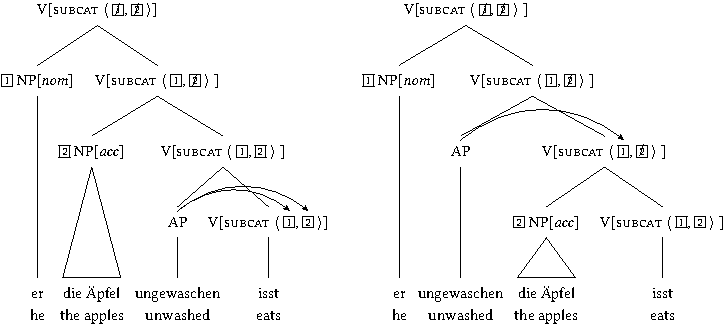
\includegraphics[width=\textwidth]{Figures/depictives-lsp-cropped.pdf}
%%  \resizebox{\linewidth}{!}{%
%% \begin{forest}
%% sn edges, for tree={l sep= 6ex}
%% [V{[\subcat \sliste{ \spirit{1}, \spirit{2} }]}
%% 	[\ibox{1} NP{[\textit{nom}]}
%% 		[er;he]]
%% 	[V{[\subcat \sliste{ \ibox{1}, \spirit{2} } ]}
%% 		[\ibox{2} NP{[\textit{acc}]}
%% 			[die Äpfel;the apples,triangle]]
%% 		[V{[\subcat \sliste{ \ibox{1}, \ibox{2} } ]}
%% 			[\subnode{ap1}{AP}
%% 				[ungewaschen;unwashed]]
%% 			[V{[\subcat \sliste{ \subnode{arg11}{\ibox{1}}, \subnode{arg12}{\ibox{2}} }]}
%% 				[isst;eats]]]]]
%% \end{forest}
%% \hspace{1em}
%% \begin{forest}
%% sn edges, for tree={l sep= 6ex}
%% [V{[\subcat \sliste{ \spirit{1}, \spirit{2} } ]}
%% 	[\ibox{1} NP{[\textit{nom}]}
%% 		[er;he]]
%% 	[V{[\subcat \sliste{ \ibox{1}, \spirit{2} } ]}
%% 		[\subnode{ap2}{AP}
%% 			[ungewaschen;unwashed]]
%% 		[V{[\subcat \sliste{ \subnode{arg21}{\ibox{1}}, \spirit{2} } ]}
%% 			[\ibox{2} NP{[\textit{acc}]}
%% 				[die Äpfel;the apples,triangle]]
%% 			[V{[\subcat \sliste{ \ibox{1}, \ibox{2} } ]}
%% 				[isst;eats]]]]]
%% \end{forest}
%% % This has to be inside of the scaling
%%     %% \begin{tikzpicture}[overlay,remember picture]
%%     %% %% this works with tikzmark
%%     %% \draw[->, bend angle=40, bend left] ($(pic cs:ap1)+(1ex,2ex)$) to($(pic cs:arg11)+(1ex,2.5ex)$);
%%     %% \draw[->, bend angle=40, bend left] ($(pic cs:ap1)+(1ex,2ex)$) to($(pic cs:arg12)+(1ex,2.5ex)$); % 1ex links, 2ex hoch
%%     %% %
%%     %% \draw[->, bend angle=40, bend left] ($(pic cs:ap2)+(1ex,2ex)$) to($(pic cs:arg21)+(1ex,2.5ex)$);
%%     %% \end{tikzpicture}
%% % somehow it stopped working
%% %% this used to work with subnode in texlive 2013 but is broken now
%% \begin{tikzpicture}[overlay,remember picture] 
%% \draw[->, bend angle=40, bend left] (ap1.north) to (arg11.north);
%% \draw[->, bend angle=40, bend left] (ap1.north) to (arg12.north); 
%% %
%% \draw[->, bend angle=40, bend left] (ap2.north) to (arg21.north);
%% \end{tikzpicture}
%}
%\hfill\mbox{}
\caption{Analysis of \emph{dass er die Äpfel ungewaschen isst} `that he the apples unwashed eats' and \emph{dass er ungewaschen die
    Äpfel isst} `that he unwashed the apples eat'}\label{anal-er-die-frau-nackt-sieht}
\end{figure}%
Arguments that have been realized are still represented on the upper nodes, however, they are crossed"=out and thereby marked as ``realized''.
In German, this preference for the antecedent noun can be captured by assuming a restriction that states that the antecedent noun must not yet have been
realized.

It is commonly assumed for English\il{English} that adjuncts are combined with a VP.
\eal
\ex John [[\sub{VP} ate the apples$_i$] unwashed$_i$].
\ex You can't [[\sub{VP} give them$_i$ injections] unconscious$_i$].\footnote{
\citew[\page 17]{Simpson2003a}.
}
\zl
In approaches where the arguments of the verb are accessible at the VP node, it is possible to establish a relation between
the depictive predicate and an argument although the antecedent noun is inside the VP.
English differs from German in that depictives can refer to both realized (\emph{them} in (\mex{0}b))
and unrealized (\emph{you} in (\mex{0}b)) arguments.

\citet[\page 560]{Higginbotham85a} and \citet{Winkler97a} have proposed corresponding non"=cancellation approaches in \gbt.
There are also parallel suggestions in Minimalist theories: checked features are not deleted, but instead marked as already
checked \citep[\page 14]{Stabler2010b}. However, these features are still viewed as inaccessible.\label{page-non-cancellation-end}

Depending on how detailed the projected information is, it can be possible to see adjuncts and argument in embedded structures as well as their
phonological, syntactic and semantic properties. In the CxG variant proposed by Kay and Fillmore, all information is available. In LFG,
information about grammatical function, case and similar properties is accessible. However, the part of speech is not contained in the f"=structure.
If the part of speech does not stand in a one"=to"=one relation to grammatical function, it cannot be restricted using selection via f"=structure.
Nor is phonological information represented completely in the f"=structure. If the analysis of idioms requires nonlocal access to phonological
information or part of speech, then this has to be explicitly encoded in the f"=structure (see \citew[\page 46--50]{Bresnan82a} for more on idioms). 

In the HPSG variant that I adopt, only information about arguments is projected. Since arguments are always represented by descriptions of type
\type{synsem}, no information about their phonological realization is present. However, there are daughters in the structure so that it is still
possible to formulate restrictions for idioms as in TAG or Construction Grammar (see \citew{RS2009a}
for an analysis of the `horse' example in (\ref{ex-ich-glaube-mich-tritt-ein-Pferd})).
This may seem somewhat like overkill: although we already have the tree structure, we are still projecting information about arguments
that have already been realized (unfortunately these also contain information about their arguments and so on). At this point, one could be inclined
to prefer TAG or LFG since these theories only make use of one extension of locality: TAG uses trees
of arbitrary or rather exactly the necessary size and LFG makes reference to a complete
f"=structure. However, things are not quite that simple: if one wants to create a relation to an
argument when adjoining a depictive predicate in TAG, then one requires a list of
possible antecedents. Syntactic factors (\eg reference to dative vs.\ accusative noun phrases, to argument vs.\ adjuncts,
coordination of verbs vs.\ nouns) play a role in determining the referent noun, this cannot be reduced to semantic relations.
Similarly, there are considerably different restrictions for different kinds of idioms and these cannot all be formulated in terms of restrictions
on f"=structure since f"=structure does not contain information about parts of speech.\is{depictive predicate|)}

One should bear in mind that some phenomena require reference to larger portions of structure. The majority of phenomena can be treated in terms of head
domains and extended head domains, however, there are idioms that go beyond the sentence level. Every theory has to account for this somehow.
\is{locality|)}\is{idiom|)}



%      <!-- Local IspellDict: en_US-w_accents -->

%% -*- coding:utf-8 -*-
\section{Recursion}
\label{sec-recursion}

Every\is{recursion|(} theory in this book can deal with self"=embedding in language as it was
discussed on page~\pageref{ex-that-max-thinks-that-recursion}. The example
(\ref{ex-that-max-thinks-that-recursion}) is repeated here as (\mex{1}):
\ea
\label{ex-that-max-thinks-that-recursion-two}
that Max thinks [that Julia knows [that Otto claims [that Karl
suspects [that Richard confirms [that Friederike is laughing]]]]]
\z
Most theories
capture this directly with recursive phrase structure rules or dominance schemata. TAG\indextag is
special with regard to recursion since recursion is factored out of the trees. The corresponding
effects are created by an adjunction operation that allows any amount of material to be inserted
into trees.  It is sometimes claimed that Construction Grammar\indexcxg cannot capture the existence
of recursive structure in natural language (\eg \citealp[\page 269]{Leiss2009a}).  This impression
is understandable since many analyses are extremely surface"=oriented. For example, one often talks
of a [Sbj TrVerb Obj] construction. However, the grammars in question also become recursive as soon
as they contain a sentence embedding or relative clause construction. A sentence embedding
construction could have the form [Sbj that-Verb that-S], where a that-Verb is one that can take
a sentential complement and that-S stands for the respective complement. A \emph{that}"=clause can then be inserted
into the that-S slot. Since this \emph{that}"=clause can also be the result of the application of
this construction, the grammar is able to produce recursive structures such as those in (\mex{1}):

\ea
Otto claims [\sub{that-S} that Karl suspects [\sub{that-S} that Richard sleeps]].
\z
In (\mex{0}), both \emph{Karl suspects that Richard sleeps} and the entire clause are instances of the [Sbj
that-Verb that-S] construction. The entire clause therefore contains an embedded subpart that is licensed by
the same construction as the clause itself. (\mex{0}) also contains a constituent of the category
\emph{that}-S that is embedded inside of \emph{that}-S. For more on recursion and self"=embedding\is{self"=embedding} in Construction Grammar, see \citew{Verhagen2010a}.

Similarly, every Construction Grammar that allows a noun to combine with a genitive\is{genitive} noun phrase also allows
for recursive structures. The construction in question could have the form [Det N
NP[gen] ] or [ N NP[gen] ]. The [Det N NP[gen] ] construction licenses structures such as (\mex{1}):
\ea
\gll [\sub{NP} des Kragens [\sub{NP} des Mantels [\sub{NP} der Vorsitzenden]]]\\
	{} the collar {} of.the coat {} of.the chairwoman\\
\glt `the collar of the coat of the chairwoman'
\z
\citet{Jurafsky96a} and \citet*{BLT2009a} use probabilistic context"=free grammars\is{context"=free grammar!probabilistic (PCFG)} (PCFG) for a Construction Grammar parser
with a focus on psycholinguistic plausibility and modeling of acquisition. Context"=free grammars
have no problems with self"=embedding\is{self"=embedding} structures like those in (\mex{0}) and thus this kind
of Construction Grammar itself does not encounter any problems with self"=embedding.

\citet[\page 192]{Goldberg95a} assumes that the resultative construction\is{construction!resultative} for English\il{English} has the following
form:
\ea
{}[SUBJ [V OBJ OBL]] 
\z
This corresponds to a complex structure as assumed for elementary trees in TAG. LTAG differs from Goldberg's approach in that every structure requires a lexical
anchor, that is, for example (\mex{0}), the verb would have to be fixed in LTAG. But in Goldberg's analysis, verbs can be inserted into independently
existing constructions (see Section~\ref{Abschnitt-Stoepselei}). In TAG publications, it is often emphasized that elementary trees do not contain any recursion.
The entire grammar is recursive however, since additional elements can be added to the tree using adjunction and -- as (\mex{-2}) and
(\mex{-1}) show -- insertion into substitution nodes can also create recursive structures.
\is{recursion|)}



%      <!-- Local IspellDict: en_US-w_accents -->


%% Here’s Chomsky’s description of this fact in his (1964:7):
%% …a mature native speaker can produce a new sentence of his language on the appropriate occasion, and other speakers can understand it immediately, though it is equally new to them. Most of our linguistic experience, both as speakers and hearers, is with new sentences; once we have mastered a language, the class of sentences with which we can operate fluently is so vast that for all practical purposes (and, obviously, for all theoretical purposes), we may regard it as infinite.


%% -*- coding:utf-8 -*-

\chapter{Empty elements}
\label{Abschnitt-Diskussion-leere-Elemente}
\label{chap-empty}

This chapter deals with empty elements, I first discuss the general attitude of various research
traditions towards empty elements and then show how they can be eliminated from grammars
(Section~\ref{Abschnitt-Eleminierung-leerer-Elemente}). Section~\ref{Abschnitt-leere-Elemente-Semantik} discusses empty elements that
have been suggested in order to facilitate semantic
interpretation. Section~\ref{Abschnitt-Evidenz-leere-Elemente} discusses possible motivation for
empty elements with a special focus on cross"=linguistic comparison and the final Section~\ref{Abschnitt-leere-Elemente-LRs-Transformations} shows
that certain accounts with transformations, lexical rules, and empty elements can be translated into each other.

\section{Views on empty elements}

One\is{empty element|(} point that is particularly controversial among proponents of the theories discussed in this book is the question of whether
one should assume empty elements or not.\todostefan{Add arguments from wanna contraction} The discussion of empty elements is quite old: there was already some investigation in 1961 with reference
to phrase structure grammars\is{phrase structure grammar} \citep*{BHPS61a}.
The discussion of the status of empty elements has carried on ever since (see
\citealp*{Loebner86a,Wunderlich87d,Wunderlich89,Stechow89,Haider97a,Sag2000a,BMS2001a,LH2006a,Mueller2004e,AS2015a}, for example). 
There are sometimes empirical differences between analyses that assume empty elements and those that
do not \citep{AS2015a}, but often this is not the case. Since empty elements often feature prominently in the argumentation for or against particular theories, I will discuss
how they have been used in somewhat more detail here.

In \gbt, empty elements were assumed for traces of movement (verb movement and fronting of phrases)
as well as for deleted elements in elliptical\is{ellipsis} constructions. Starting with the analysis
of \citet{Larson88a}, more and more empty heads have been introduced to ensure
uniformity\is{uniformity} of structures and certain semantic interpretations (binding\is{Binding
  Theory} and scope\is{scope}, see Section~\ref{sec-little-v} on \littlev). Other examples of an
empty element that was introduced in order to maintain particular generalizations are the empty
expletives\is{pronoun!expletive} of \citet[\page 734]{Coopmans-89a-u} and
\citet[Chapter~1]{Postal2004a-u}. These fill the subject position in inversion\is{inversion}
structures in English\il{English}, where the position preceding the verb is occupied by a PP and not
by an overt subject NP. 
% Bresnan94a zitiert: Dutch (Maling & Zaenen 1978, Perlmutter & Zaenen 1984), Icelandic and Faroese (Platzack 1987)
Similarly, \citet[Section~4]{Safir85a-u} assumes that impersonal passives\is{passive!impersonal} in German contain empty
expletive subjects. \citet[\page 1311]{Grewendorf93} assumes that the subject
position in impersonal passives\is{passive!impersonal} and passives without subject movement is in
fact occupied by an empty expletive. Also, see \citew[\page 91]{Newmeyer2005a} and \citet[\page
  180]{Lohnstein2014a} for this assumption with regard to the passive in
German. \citet[Section~II.3.3.3]{Sternefeld2006a-u} assumes that there is an empty expletive subject
in impersonal passives and subjectless sentences such as (\mex{1}).
\eal
\ex 
\gll Mir graut.\\
	 me.\dat{} scares\\
\glt `I am scared.'
\ex 
\gll Mich dürstet.\\
	 me.\acc{} is.thirsty\\
\glt `I am thirsty.'
\zl

\noindent
On page~\pageref{Beispiel-leeres-Element-intransitive-Verben}, we discussed Stabler's proposal for the analysis of sentences with intransitive
verbs. Since, following  \citet[\page 146]{Chomsky2008a}, the element that first merges with a head is the complement, intransitive verbs pose a problem for the
theory. This problem is solved by Stabler by assuming that intransitive verbs are combined with an empty object \citep[\page 61,
124]{Veenstra98a}. Since these silent elements do not contribute to the meaning of an expression, we are also dealing with empty expletive pronouns.

\addlines
In other theories, there are researchers that reject empty elements as well as those who assume them.
In Categorial Grammar\indexcg, Steedman suggests an analysis of nonlocal dependencies that does
without empty elements (see Section~\ref{sce-nld-cg}), but as \citet{Pollard88a} has shown,
Steedman's analysis requires various kinds of type raising\is{type raising}
for NPs or a correspondingly high number of complex lexical items for relative
pronouns\is{pronoun!relative} (see Section~\ref{Abschnitt-CG-UDC}). On the other hand, 
\citet{Koenig99a-u} uses\todostefan{andere Quellen?} traces. In GPSG\indexgpsg, there is the
trace"=less analysis of extraction\is{extraction} by \citet[\page 76--77]{Uszkoreit87a} that we
discussed in  Section~\ref{Abschnitt-GPSG-Fernabhaengigkeiten}, but there is also the analysis of
\citet*[\page 143]{GKPS85a} that uses traces. In LFG\indexlfg, there are both analyses with traces
\citep[\page 67]{Bresnan2001a} and those without (see \citew{KZ89a,DKK2001a-u} and
Section~\ref{Abschnitt-Verbstellung-LFG} and Section~\ref{Abschnitt-NLA-LFG}).  
Many of the phrasal analyses in HPSG\indexhpsg are born out of the wish to avoid empty elements (see Section~\ref{Abschnitt-Phrasale-Konstruktionen}). 
An example for this is the relative clause analysis by \citet{Sag97a} that replaces the empty
relativizer in \citew{ps2} with a corresponding phrasal rule. On the other hand we have
\citew{Bender2000a} and \citew*[\page 464]{SWB2003a}, who assume a silent copula\is{copula},
\citew{Borsley99c-u,Borsley2009a-u,Borsley2013a-u}, who argues for empty elements in the grammar of Welsh\il{Welsh} and \citet{AB2012a}, who suggest an empty relativizer for Arabic\il{Arabic}. Another
attempt to eliminate empty elements from HPSG was to handle long"=distance dependencies not by
traces but rather in the lexicon \citep*{BMS2001a}. As \citet{LH2006a} could show, however, theories
of extraction that introduce long"=distance dependencies lexically have problems with the semantic
interpretation of coordinate structures. For a suggestion of how to solve these problems, see
\citew{Chaves2009a}. There are many TAG analyses\indextag without silent elements in the lexicon
(see Section~\ref{TAG-Fernabh} and \citew{Kroch87a}, for example), however there are variants of TAG
such as that of \citet[\page 194]{Kallmeyer2005a-u}, where a trace is assumed for the reordering of
constituents in sentences with a verbal complex. \citet[\page 10--11]{Rambow94a} assumes an empty head in every verb
phrase (see Section~\ref{sec-vtag} on V"=TAG\is{Tree Adjoining Grammar (TAG)!Vector (V-TAG)}).\footnote{
  Note that empty elements in TAG are slightly different from empty elements in other theories. In
  TAG the empty elements are usually part of elementary trees, that is, they are not lexical items that are
  combined with other material.
}
In Dependency Grammar, \mel (\citeyear[\page 303]{Melcuk88a-u}; \citeyear[\page 219]{Melcuk2003a-u}),
%\todostefan{S: It is possible to introduce empty nodes in a DT if you want. It has been done for
%  gapping by Tesnière or for agreement by Melcuk (1988:303)}
%\todostefan{O: Starosta 1988:253, Eroms 2000:472, Melcuk 2003:219, Hudson (2007:172-182, 2010)}
\citet[\page 253]{Starosta88a-u}, \citet[\page 471--472]{Eroms2000a}, Hudson (\citeyear[Section~3.7]{Hudson2007a-u}; \citeyear[\page 166]{Hudson2010a-u}) and
\citet{Engel2014a} assume empty elements for determiners, nouns, ellipsis, imperatives, controlled infinitives, and for coordinate
structures, but \citet[\page 73]{GO2009a} reject empty elements (with the exception of ellipsis, \citealp{Osborne2016a-u}).

No empty elements are assumed in Construction Grammar\indexcxg\label{Seite-leere-Elemente-CxG} (\citealp[\page 49--50]{MR2001a}; \citealp[\page
219]{Goldberg2003b}; \citealp[\page 10]{Goldberg2006a}), the related Simpler Syntax \citep{CJ2005a} as well as in Cognitive Grammar\is{Cognitive Grammar}.\footnote{
  However, \citet[\page 51]{Fillmore88a} did not rule them out.
} 
The argumentation against empty elements runs along the following lines:
\begin{enumerate}
\item There is no evidence for invisible objects.
\item There is no innate linguistic knowledge.
\item Therefore, knowledge about empty elements cannot be learned, which is why they cannot be assumed
as part of our grammar.
\end{enumerate}
This begs the question of whether all the premises on which the conclusion is based actually hold. If we consider an elliptical
construction such as (\mex{1}), then it is clear that a noun has been omitted:
\ea
\gll Ich nehme den roten Ball und du den blauen.\\
	 I take the.\acc{} red.\acc{} ball and you the.\acc{} blue.\acc{}\\
\glt `I'll take the red ball and you take the blue one.'
\z
Despite there being no noun in \emph{den blauen} `the blue', this group of words behaves both syntactically and semantically just like a noun
phrase. (\mex{0}) is of course not necessarily evidence for there being empty elements, because one could simply say that \emph{den blauen}
is a noun phrase consisting only of an article and an adjective \citep{Wunderlich87d}. 

Similar to the fact that it is understood that a noun is missing in (\mex{0}), speakers of English know that something is missing after
\emph{like}: 
\ea
Bagels, I like.
\z
Every theory of grammar has to somehow account for these facts. It must be represented in some way that \emph{like} in (\mex{0}) behaves
just like a verb phrase that is missing something. One possibility is to use traces. \citet*[\page 153, Lemma~4.1]{BHPS61a} 
have shown that it is possible to turn phrase structure grammars with empty elements into those without any.
In many cases, the same techniques can be applied to the theories presented here and we will therefore discuss the point in more detail
in the following section.

\section{Eliminating empty elements from grammars}
\label{Abschnitt-Eleminierung-leerer-Elemente}

It is possible to turn a grammar with empty elements (also called \emph{epsilon}\is{epsilon}) into a
grammar without these by removing all categories that can be rewritten by an epsilon in every rule
that uses such categories and then add the respective rules without the empty elements to the grammar. The following example has an epsilon rule for np. One therefore has to
replace all rules containing the symbol np with new rules without this np symbol. (\mex{2}) shows
the result of this conversion of the grammar in (\mex{1}):

\ea
\label{ex-grammar-eps-head}
\begin{tabular}[t]{@{}l@{~$\to$~}l@{}}
\baro{v}   & \mbox{np}, v\\
\baro{v}   & \mbox{np}, pp, v\\
np & $\epsilon$\\
\end{tabular}
\z

\ea
\label{ex-grammar-head}
\begin{tabular}[t]{@{}l@{~$\to$~}l@{}}
\baro{v}   & \mbox{np}, v\\
\baro{v}   & v\\
\baro{v}   & \mbox{np}, pp, v\\
\baro{v}   & \mbox{pp}, v\\
\end{tabular}
\z
This can also lead to cases where all elements on the right"=hand side of a rule are removed. Thus,
what one has done is actually create a new empty category and then one has to apply the respective
replacement processes again. We will see an example of this in a moment. Looking at the pair of
grammars in (\mex{-1})--(\mex{0}), it is clear that the number of rules has increased in (\mex{0})
compared to (\mex{-1}) despite the grammars licensing the same sequences of symbols. The fact that
an NP argument can be omitted is not expressed directly in (\mex{0}) but instead is implicitly contained in two rules. 

If one applies this procedure to the HPSG\indexhpsg grammar in Chapter~\ref{Kapitel-HPSG}, then the
trace does not have a specific category such as NP. The trace simply has to be compatible with a
non"=head daughter. As the examples in (\mex{1}) show, adjuncts, arguments and parts of verbal
complexes can be extracted.
\eal
\ex 
\gll Er$_i$ liest t$_i$ die Berichte.\\
	 he reads {}    the reports\\
\ex 
\gll Oft$_i$ liest er die Berichte t$_i$ nicht.\\
	 often reads he the reports {} not\\
\glt `Often, he does not read the reports.'
\ex 
\gll Lesen$_i$ wird er die Berichte t$_i$ müssen.\\
	 read will he the reports {} must\\
\glt `He will have to read the reports.'
\zl

\noindent
The relevant elements are combined with their head in a specific schema (Head"=Argument Schema, Head"=Adjunct Schema,
Predicate Complex Schema). See Chapter~\ref{Kapitel-HPSG} for the first two schemata; the Predicate Complex Schema is
motivated in detail in Müller (\citeyear[Chapter~2]{Mueller2002b};
\citeyear[Chapter~15]{MuellerLehrbuch1}). If one wishes to do without traces, then one needs further additional schemata for the fronting of adjuncts, of arguments and of parts of predicate
complexes. The combination of a head with a trace is given in Figure~\vref{Abbildung-Kopf+Spur}. The
trace"=less analysis is shown in Figure~\vref{Abbildung-Kopf-ohne-Spur}.
\begin{figure}
\centering
\begin{forest}
sm edges
[ V\feattab{\subcat \sliste{ NP[\type{nom}] },\\
             \textsc{inher$|$slash} \sliste{ \ibox{1} }}\\
  [{\ibox{4} \feattab{
                \textsc{loc} \ibox{1},\\
                \textsc{inher$|$slash} \sliste{ \ibox{1} }}} [\trace]]
  [V\feattab{
                \subcat \sliste{ NP[\type{nom}], \ibox{4} NP[\type{acc}] }} [liest;reads]]]
\end{forest}
\caption{\label{Abbildung-Kopf+Spur}Introduction of information about long"=distance dependencies with a trace}
\end{figure}%
In Figure~\ref{Abbildung-Kopf+Spur}, the element in the \subcatl of \emph{kennen} is identified with the \synsemv of the trace \ibox{4}.
The lexical entry of the trace prescribes that the \locv of the trace should be identical to  the element in the \textsc{inher$|$slash} list.

The Non"=Local Feature Principle (page~\pageref{Prinzip-der-Nichtlokalen-Merkmale}) ensures that the \slasch information is present on the
mother node. Since an argument position gets saturated in Head"=Argument structures, the accusative object is no longer contained in the
\subcatl of the mother node.

Figure~\ref{Abbildung-Kopf-ohne-Spur} shows the parallel trace"=less structure.
\begin{figure}
\centering
\begin{forest}
sm edges
[{V\feattab{
                                    \subcat \sliste{ NP[\type{nom}] },\\
                                    \textsc{inher$|$slash} \sliste{ \ibox{1} } }}\\
    [V\feattab{
                                             \subcat \sliste{ NP[\type{nom}], NP\ibox{1}[\type{acc}] }}\\
          [liest;reads]]]
\end{forest}
\caption{\label{Abbildung-Kopf-ohne-Spur}Introduction of information about long"=distance dependencies using a unary projection}
\end{figure}%
The effect that one gets by combining a trace in argument position in Head"=Argument structures is represented directly
on the mother node in Figure~\ref{Abbildung-Kopf-ohne-Spur}: the \locv of the accusative object was identified with the element in
\textsc{inher$|$slash} on the mother node and the accusative object does not occur in the valence list any more.

\largerpage
The grammar presented in Chapter~\ref{Kapitel-HPSG} contains another empty element: a verb trace. This would then also have to be
eliminated.

\eal
\ex 
\gll Er$_i$ liest$_j$ t$_i$ die Berichte t$_j$.\\
	 he reads {}    the reports\\
\ex 
\gll Oft$_i$ liest$_j$ er die Berichte t$_i$ nicht t$_j$.\\
	 often reads he the reports {} not\\
\glt `Often, he does not read the reports.'
\ex 
\gll Lesen$_i$ wird$_j$ er die Berichte t$_i$ müssen t$_j$.\\
	 read will he the reports {} must\\
\glt `He will have to read the reports.'
\zl

\noindent
Figure~\vref{Abbildung-Kopf+Verbspur} shows the combination of a verb trace with an accusative object.
\begin{figure}
\centering
\begin{forest}
sm edges
[V\feattab{
                                    \textsc{head$|$dsl} \ibox{1},\\
                                    \subcat \ibox{2} }
   [{\ibox{3} NP[\type{acc}]}
     [ die Berichte;the reports, roof] ]
   [V\ibox{1}\feattab{
                    \textsc{head$|$dsl} \ibox{1},\\
                    \subcat \ibox{2} $\oplus$ \sliste{ \ibox{3} NP[\type{acc}] }} 
     [\trace]]]
\end{forest}
\caption{\label{Abbildung-Kopf+Verbspur}Analysis of verb position with verb trace}
\end{figure}%
The verb trace is specified such that the \dslv is identical to the \locv of the trace (see
p.\,\pageref{le-verbspur}). Since \dsl is a head feature, the corresponding value is also present on
the mother node. Figure~\vref{Abbildung-Kopf-ohne-Verbspur} shows the structures that we get by omitting the empty node.
\begin{figure}
\centering
\begin{forest}
sm edges, for tree={l sep= 5ex}
[ V\feattab{
     \textsc{head$|$dsl} V[\subcat \ibox{2} $\oplus$ \sliste{ \ibox{3} NP[\type{acc}] }],\\
     \subcat \ibox{2}} 
   [{\ibox{3} NP[\type{acc}]}
      [die Berichte;the reports, roof]]]
\end{forest}
\caption{\label{Abbildung-Kopf-ohne-Verbspur}Analysis of verb position using a unary projection}
\end{figure}%
This structure may look odd at first sight since a noun phrase is projected to a verb (see page~\pageref{Abb-Verbstellung-LFG} 
for similar verb"=less structures in LFG\indexlfg). The information about the fact that a verb is missing in the structure
is equally contained in this structure as in the structure with the verb trace. It is the \dslv that is decisive for the contexts in which
the structure in Figure~\ref{Abbildung-Kopf-ohne-Verbspur} can appear. This is identical to the value in Figure~\ref{Abbildung-Kopf+Verbspur} and contains
the information that a verb that requires an accusative object is missing in the structure in question.
Until now, we have seen that extraction traces can be removed from the grammar by stipulating three additional rules. Similarly, three new rules
are needed for the verb trace. Unfortunately, it does not stop here as the traces for extraction and
head movement can also interact. For example, the NP in the tree in 
Figure~\ref{Abbildung-Kopf-ohne-Verbspur} could be an extraction trace. Therefore, the combination of traces can result in more empty elements that then
also have to be eliminated. Since we have three schemata, we will have three new empty elements if we combine the non"=head daughter with an extraction
trace and the head daughter with a verb trace. (\mex{1}) shows these cases:
\eal\settowidth\jamwidth{(Extraction trace (argument) $+$ verb trace)}
\ex 
\gll Er$_i$    [schläft$_j$ t$_i$ t$_j$].\\
	 he \spacebr{}sleeps\\  \jambox{(Extraction trace (argument) $+$ verb trace)}
\glt `He is sleeping.'
\ex 
\gll Jetzt$_i$ [schlaf$_j$ t$_i$ t$_j$]!\\
	 now \spacebr{}sleep\\   \jambox{(Extraction trace (adjunct)  $+$ verb trace)}
\glt `Go to sleep now!'
\ex 
\gll Geschlafen$_i$ [wird$_j$ t$_i$ t$_j$]! \\
	 slept \spacebr{}is\\\jambox{(Extraction trace (complex) $+$ verb trace)}
\glt `Now is time to sleep!'
\zl
These three new traces can occur as non"=head daughters in the Head"=Argument Schema and thus one would require
three new schemata for Head"=Argument structures. Using these schemata, it then becomes possible to analyze
the sentences in (\mex{0}).

Six further schemata are required for the examples in (\mex{1}) and (\mex{2}) since the three new traces can each occur
as heads in Head"=Argument structures (\mex{1}) and Head"=Adjunct structures (\mex{2}):
\eal
\ex 
\gll Den Aufsatz$_i$ liest$_j$ [er t$_i$ t$_j$].\\
	 the essay reads \spacebr{}he\\
\glt `He is reading the essay.'
\ex 
\gll Oft$_i$ liest$_j$ er [ihn t$_i$ t$_j$].\\
	 often reads he \spacebr{}it\\
\glt `He often reads it.'
\ex 
\gll Lesen$_i$ wird$_j$ er [ihn t$_i$ t$_j$].\\
	 read will he \spacebr{}it\\
\glt `He will read it.'
\zl
\eal
\ex 
\gll Den Aufsatz$_i$ liest$_j$ er [nicht t$_i$ t$_j$].\\
	 the essay reads he \spacebr{}not\\
\glt `He isn't reading the essay.'
\ex 
\gll Oft$_i$ liest$_j$ er ihn [nicht t$_i$ t$_j$].\\
	 often reads he it \spacebr{}not\\
\glt `He often doesn't read it'
\ex 
\gll Lesen$_i$ wird$_j$ er ihn [nicht t$_i$ t$_j$].\\
	 reads will he it \spacebr{}not\\
\glt `He won't read it.'
\zl
\largerpage
Eliminating two empty elements therefore comes at the price of twelve new rules. These rules are not particularly transparent and it is not immediately
obvious why the mother node describes a linguistic object that follows general grammatical laws. For example, there are no heads in the structures following
the pattern in Figure~\ref{Abbildung-Kopf-ohne-Verbspur}. Since there is no empirical difference between the theoretical variant with twelve
additional schemata and the variant with two empty elements, one should prefer the theory that makes fewer assumptions (Occam's Razor) and that
is the theory with two empty elements.

One might think that the problem discussed here is just a problem specific to HPSG not shared by trace"=less analyses such as the LFG\indexlfgstart approach
that was discussed in Section~\ref{Abschnitt-NLA-LFG}. If we take a closer look at the rule proposed
by \citet[\page 84]{Dalrymple2006a}, we see that the situation in LFG grammars is entirely
parallel. The brackets around the category symbols mark their optionality. The asterisk following
the PP means that any number of PPs (zero or more) can occur in this position.
\ea
V$'$ $\to$ (V) (NP) PP*
\z
This means that (\mex{0}) is a shorthand for rules such as those in (\mex{1}):
\eal
\ex V$'$ $\to$ V
\ex V$'$ $\to$ V NP
\ex V$'$ $\to$ V NP PP
\ex V$'$ $\to$ V NP PP PP
\ex \ldots
\ex V$'$ $\to$ NP
\ex V$'$ $\to$ NP PP
\ex V$'$ $\to$ NP PP PP
\ex \ldots
\zl
Since all the elements on the right"=hand side of the rule are optional, the rule in (\mex{-1}) also stands for (\mex{1}):
\ea
V$'$ $\to$ $\epsilon$
\z
\addlines
Thus, one does in fact have an empty element in the grammar although the empty element is not explicitly listed in the lexicon.
This follows from the optionality of all elements on the right"=hand side of a rule. The rule in (\mex{-1}f) corresponds
to the schema licensed by the structure in Figure~\ref{Abbildung-Kopf-ohne-Verbspur}. In the licensed LFG structure, there is 
also no head present. Furthermore, one has a large number of rules that correspond to exactly the schemata that we get when
we eliminate empty elements from an HPSG grammar. This fact is, however, hidden in the representational format of the LFG rules.
The rule schemata of LFG allow for handy abbreviations of sometimes huge sets of rules (even infinite sets when using `*').\indexlfgend

\citet{Pollard88a} has shown that Steedman's trace"=less analysis of long"=distance dependencies is not without its problems.
As discussed in Section~\ref{Abschnitt-CG-UDC}, a vast number of recategorization rules or lexical entries for
relative pronouns are required.

\section{Empty elements and semantic interpretation}
\label{Abschnitt-leere-Elemente-Semantik}
\label{sec-MRS-wieder}

In this section, I discuss an analysis that assumes empty elements in order to allow for different readings of particular sentences. I then show how
one can use so"=called underspecification approaches to do without empty elements.

Sentences such as (\mex{1}) are interesting since they have multiple readings (see \citealp[Section~5.6]{Dowty79a}) and it is not obvious
how these can be derived.
\ea
\label{ex-alle-wieder}
\gll dass Max alle Fenster wieder öffnete\\
	 that Max all windows again opened\\
\glt `that Max opened all the windows again'
\z
There is a difference between a repetitive\is{repetitive} and a restitutive\is{restitutive} reading: for the repetitive reading of
(\mex{0}), Max has to have opened every window at least once before, whereas the restitutive reading only requires that all windows were open
at some point, that is, they could have been opened by someone else.

These different readings are explained by decomposing the predicate \relation{open} into at least two sub"=predicates.
\citet{Egg99a} suggests the decomposition into CAUSE\is{CAUSE} and \relation{open}:
\ea
CAUSE(x, \relation{open}(y))
\z
This means that there is a CAUSE operator that has scope over the relation \relation{open}.
Using this kind of decomposition, it is possible to capture the varying scope of \emph{wieder} `again':
in one of the readings, \emph{wieder} scopes over CAUSE and it scopes over \relation{open} but below
CAUSE in the other. If we assume that \emph{öffnen} has the meaning in (\mex{0}), then we still have to explain how the adverb
can modify elements of a word's meaning, that is, how \emph{wieder} `again' can refer to \relation{open}.
\Citet[\page 93]{Stechow96a} developed the analysis in Figure~\vref{Abbildung-wieder-oeffnen-Stechow}.
\begin{figure}
\centering
\begin{forest}
no word baseline
[AgrSP
	[DP
		[Max$_ i$;Max,tier=word]]
	[AgrS$'$
		[TP
			[AgrOP
				[DP
					[alle Fenster$_ j$;all windows,roof,tier=word]]
				[AgrO$'$
					[VoiceP
						[DP
							[t$_i$,tier=word]]
						[Voice$'$
							[Voice
								[CAUSE,tier=word]]
							[VP
								[XP
									[t$_j$,tier=word]
									[offen;open,tier=word]]
								[V
									[BECOME,tier=word]]]]]
					[AgrO]]]
			[T]]
		[AgrS]]]
\end{forest}
\caption{\label{Abbildung-wieder-oeffnen-Stechow}Decomposition in syntactic structures}
\end{figure}%
AgrS\is{category!functional!AgrS} and AgrO\is{category!functional!AgrO} are functional heads
proposed for subject and object agreement\is{agreement!object} in languages like Basque\il{Basque} and
have been adopted for German (see Section~\ref{Abschnitt-neues-GB}). Noun phrases have to be moved from the VoiceP\is{category!functional!Voice} into the specifier
position of the AgrS and AgrO heads in order to receive case.
T\is{category!functional!T} stands for Tense and corresponds to Infl in the \gbt (see
Section~\ref{sec-GB-CP-IP-System-English} and Section~\ref{sec-CP-TP-vP-VP}). 
What is important is that there is the Voice head and the separate representation of \emph{offen} `open' as the head of its
own phrase. In the figure, everything below Voice$'$ corresponds to the verb \emph{öffnen}. By assuming a separate Voice head that
contributes causative meaning, it becomes possible to derive both readings in syntax: in the reading with narrow scope of \emph{wieder} `again',
the adverb is adjoined to the XP and has scope over open(x). In the reading with wide scope, the adverb attaches to VoiceP or some higher phrase
and therefore has scope over CAUSE(BECOME(open(x))).

\citet{JB2003a-u} point out that this analysis predicts that sentences such as (\mex{1}) only have the repetitive reading, that is, the reading where 
\emph{wieder} `again' has scope over CAUSE.
\ea
\label{ex-wieder-alle}
\gll dass Max wieder alle Fenster öffnete\\
     that Max again all windows opened\\
\z
This is because \emph{wieder} precedes \emph{alle Fenster} and therefore all heads that are inside VoiceP. Thus, \emph{wieder} can only
be combined with AgrOP or higher phrases and therefore has (too) wide scope. (\mex{0}) does permit a restitutive reading, however:
all windows were open at an earlier point in time and Max reestablishes this state.

\citet{Egg99a} develops an analysis for these \emph{wieder} cases using Constraint
  Language for Lambda"=Structures (CLLS)\is{Constraint Language for Lambda"=Structures (CLLS)}.
CLLS is an underspecification formalism\is{underspecification}, that is, no logical formulae are given but instead expressions that
describe logical formulae. Using this kind of expressions, it is possible to leave scope relations underspecified. I have already mentioned Minimal Recursion
Semantics (MRS)\indexmrs \citep*{CFPS2005a} in several chapters of this book. As well as CLLS, MRS
together with Underspecified Discourse Representation Theory\is{Underspecified Discourse Representation Theory (UDRT)}
  \citep{Reyle93b-u,FR95a-u} and Hole Semantics\is{Hole Semantics} \citep{Bos96a-u,BB2005a} all belong to the class
  of underspecification formalisms. See  \citew{BK2002a-u} for an underspecification analysis in Categorial Grammar\indexcg and 
\citew{Nerbonne93a} for an early underspecification analysis in HPSG\indexhpsg. In the following, I
will reproduce Egg's analysis in an MRS"=like notation.\todostefan{Kallmeyer: MRS erlaubt nur Quantoren in qeq-Ausdrücken, d.h. im strengen Sinne
    ist das hier keine MRS.}

\addlines
Before we turn to (\ref{ex-alle-wieder}) and (\ref{ex-wieder-alle}), let us consider the simpler sentence in (\mex{1}):
\ea
\gll dass Max alle Fenster öffnete\\
	 that Max all windows opened\\
\glt `that Max opened all the windows'
\z
This sentence can mean that in a particular situation, it is true of all windows that Max opened them.
A less readily accessible reading is the one in which Max causes all of the windows to be open. It is possible
to force this reading if one rules out the first reading through contextual information \citep{Egg99a}:
\ea
\gll Erst war nur die Hälfte der Fenster im Bus auf, aber dann öffnete Max alle Fenster.\\
     first was only the half of.the windows in.the bus open but then opened Max all windows\\
\glt `At first, only half of the windows in the bus were open, but then Max opened all of the windows.'
\z
Both readings under discussion here differ with regard to the scope of the universal quantifier. The reading where
Max opens all the windows himself corresponds to wide scope in (\mex{1}a). The reading where some windows could
have already been open corresponds to (\mex{1}b):
\eal
\ex $\forall$ x \relation{window}(x) $\to$ CAUSE(\relation{max}, \relation{open}(x))
\ex CAUSE(\relation{max}, $\forall$ x \relation{window}(x) $\to$ \relation{open}(x))
\zl
Using underspecification, both of these readings can be represented in one dominance graph such as
the one given in Figure~\vref{Abbildung-Max-alle-Fenster-oeffnete}.
\begin{figure}
\centering
%% broken with texlive 2015
%% \begin{tabular}{@{}ccc@{}}
%%                                & \mysubnode{h0}{h0}                & \\[8ex]
%% \mynode{h1}{h1:every(x, \mynode{h2}{h2}, \mynode{h3}{h3})}      &                              & \mynode{h6}{h6:CAUSE(max, \mynode{h7}{h7})}\\[8ex]
%% \mynode{h4}{h4:window(x)}           &          & \\[6ex]
%%                                & \mynode{h5}{h5:open(x)}\\
%% \end{tabular}
%% \begin{tikzpicture}[overlay,remember picture,dashed]
%% \draw(h0.south)--(h1.north); 
%% \draw(h0.south)--(h6.north);
%% \draw(h2.south)--(h4.north);
%% \draw(h3.south)--(h5.north);
%% \draw(h7.south)--(h5.north);
%% \end{tikzpicture}
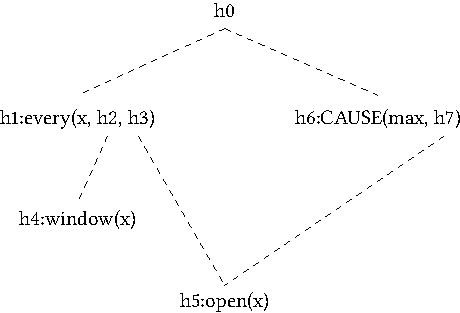
\includegraphics{Figures/max-alle-fenster-oeffnete-mrs-cropped.pdf}
\caption{Dominance graph for \emph{Max alle Fenster öffnete}\label{Abbildung-Max-alle-Fenster-oeffnete}}
\end{figure}%
Each relation in Figure~\ref{Abbildung-Max-alle-Fenster-oeffnete} has a name that one can use to refer to the relation or ``grasp'' it.
These names are referred to as \emph{handle}. The dominance graph states that $h0$ dominates both $h1$ and $h6$ and that
$h2$ dominates $h4$, $h3$ dominates $h5$, and $h7$ dominates $h5$. The exact scopal relations are underspecified: the universal quantifier can have scope over
CAUSE or CAUSE can have scope over the universal quantifier. Figures~\ref{fig-alle-cause} and
\ref{fig-cause-alle} show the variants of the graph with resolved scope.
\begin{figure}
\centering
%% \begin{tabular}{@{}ccc@{}}
%%                                & \mybox[h0]{h0}                & \\[8ex]
%% \mybox[h1]{h1:every(x, \mybox[h2]{h2}, \mybox[h3]{h3})}      &                              & \mybox[h6]{h6:CAUSE(max, \mybox[h7]{h7})}\\[8ex]
%% \mybox[h4]{h4:window(x)}           &         & \\[6ex]
%%                                & \mybox[h5]{h5:open(x)}\\
%% \end{tabular}

%% \begin{tikzpicture}[overlay,remember picture] 
%% \draw(h0.south)--(h1.north); 
%% \draw(h2.south)--(h4.north);
%% \draw(h3.south) .. controls +(0,-1) and +(-1,1)..  (h6.north);
%% \draw(h7.south)--(h5.north);
%% \end{tikzpicture}
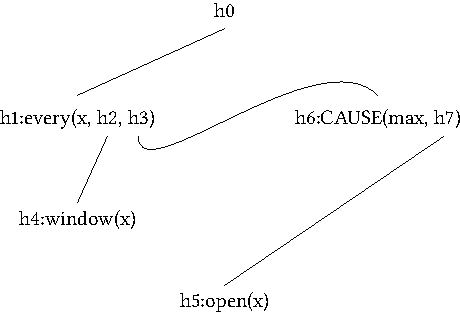
\includegraphics{Figures/solution-mrs-all-cause-open-cropped.pdf}
\caption{Dominance graph for the reading $\forall$ x window(x) $\to$ CAUSE(max,open(x)).\label{fig-alle-cause}}
\end{figure}%
\begin{figure}
\centering
%% \begin{tabular}{@{}ccc@{}}
%%                                & \mybox[h0]{h0}                & \\[8ex]
%% \mybox[h1]{h1:every(x, \mybox[h2]{h2}, \mybox[h3]{h3})}      &                              & \mybox[h6]{h6:CAUSE(max, \mybox[h7]{h7})}\\[8ex]
%% \mybox[h4]{h4:window(x)}           &          & \\[6ex]
%%                                & \mybox[h5]{h5:open(x)}\\
%% \end{tabular}

%% \begin{tikzpicture}[overlay,remember picture] 
%% \draw(h0.south)--(h6.north); 
%% \draw(h7.south) .. controls +(0,-1) and +(-1,1)..  (h1.north);
%% \draw(h2.south)--(h4.north);
%% \draw(h3.south)--(h5.north);
%% \end{tikzpicture}
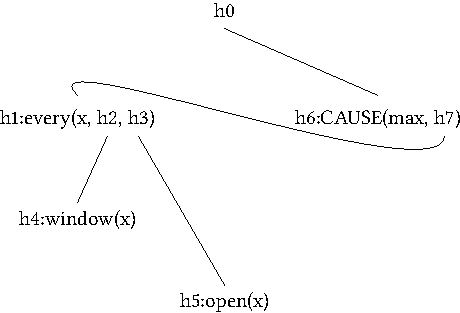
\includegraphics{Figures/solution-mrs-cause-all-open-cropped.pdf}
\caption{Graph for te reading CAUSE(max, $\forall$ x window(x) $\to$ open(x)).\label{fig-cause-alle}}
\end{figure}%
The underspecified graph in Figure~\ref{Abbildung-Max-alle-Fenster-oeffnete} does not say anything
about the relation between $h3$ and $h6$. The only thing it says is that $h3$ somehow has to dominate
$h5$. In Figure~\ref{fig-alle-cause} every ($h3$) dominates CAUSE ($h6$) and CAUSE dominates open
($h5$). So, \relation{every} dominates \relation{open} indirectly. In Figure~\ref{fig-cause-alle}, CAUSE
dominates \relation{every} and \relation{every} dominates \relation{open}. Again the constraints of
Figure~\ref{Abbildung-Max-alle-Fenster-oeffnete} are fulfilled, but $h7$ dominates $h5$ only indirectly.

The fact that the quantifier dominates $h4$ is determined by the lexical entry of the quantifier. The fact that
the quantifier dominates $h5$ does not have to be made explicit in the analysis since the quantifier binds a variable
in the relation belonging to $h5$, namely x. The dominance relation between $h7$ and $h5$ is always determined in the lexicon
since CAUSE and \relation{open}  both belong to the semantic contribution of a single lexical entry.

The exact syntactic theory that one adopts for this analysis is, in the end, not of great importance.
I have chosen HPSG here. As Figure~\vref{Abbildung-Fenster-oeffnete-MRS} shows, the analysis of \emph{alle Fenster öffnet}
contains a simple structure with a verb and an object.
\begin{figure}
%\begin{sideways}
\oneline{%
\begin{forest}
sm edges, for tree={l sep= 4ex}
[V$'$\feattab{
    \subcat \sliste{ NP\ind{y} },\\
    \rels \relliste{ h1:every(x, h2, h3), h4:window(x), h6:CAUSE(y,h7), h5:open(x) },\\
    \hcons \relliste{ h0 \qeq h1, h2 \qeq h4, h0 \qeq h6, h7 \qeq h5 }    }
  [\ibox{2} NP\ind{x}\feattab{
    \rels \relliste{ h1:every(x, h2, h3), h4:window(x) },\\
    \hcons \relliste{ h0 \qeq h1, h2 \qeq h4 } } 
    [Det\feattab{
    \rels \relliste{ h1:every(x, h2, h3) },\\
    \hcons \relliste{ h0 \qeq h1, h2 \qeq h4  } } [alle] ]
    [N\feattab{
    \rels \relliste{ h4:window(x) },\\
    \hcons \relliste{ } } [Fenster] ] ]
  [V\feattab{
                                           \subcat \sliste{ NP\ind{y}, \ibox{2} },\\
                                           \rels \relliste{ h6:CAUSE(y,h7), h5:open(x) },\\
                                           \hcons \relliste{ h0 \qeq h6, h7 \qeq h5 } } [öffnete] ]
]
\end{forest}
}
%\end{sideways}
\caption{\label{Abbildung-Fenster-oeffnete-MRS}MRS analysis of \emph{alle Fenster öffnete}}
\end{figure}%
This structure does not differ from the one that would be assumed for \emph{alle Kinder kennt} `all
children know', involving the semantically simplex verb \emph{kennen} `to know'.
The only difference comes from the meaning of the individual words involved.
As shown in Section~\ref{Abschnitt-HPSG-Semantik}, relations between individual words are passed on upwards.
The same happens with scopal restrictions. These are also represented in lists. \hcons stands for \emph{handle constraints}.
\qeq in h0 \qeq h6 stand for the equality \emph{modulo} quantifier scope.

Egg lists the following readings for the sentence in (\ref{ex-wieder-alle}) -- repeated here as (\mex{1}):
\ea
\label{ex-wieder-alle-zwei}
\gll dass Max wieder alle Fenster öffnete\\
	 that Max again all windows opened\\
\glt `that Max opened all the windows again'
\z
\begin{enumerate}
\item Max opened every window and he had already done that at least once for each window
      (\relation{again}($\forall$(CAUSE(open))); repetitive)
\item Max caused every window to be open and he had done that at least once before 
      (\relation{again}(CAUSE($\forall$(open))); repetitive)
\item At some earlier point in time, all windows were simultaneously open and Max re-established this state
      (CAUSE(\relation{again}($\forall$(open))); restitutive)
\end{enumerate}

\noindent
These readings correspond to the dominance graph in Figure~\vref{Abbildung-Max-wieder-alle-Fenster-oeffnete}.
\begin{figure}
\centering
%%   \begin{tabular}{@{}ccc@{}}
%%   & \mybox[h0]{h0}                       & \\[4ex]
%%     \mybox[h8]{h8:again}\mybox[h9]{(h9)}  \\[4ex]
%%     \mybox[h1]{h1:every(x, \mybox[h2]{h2}, \mybox[h3]{h3})}      &                              & \mybox[h6]{h6:CAUSE(max, \mybox[h7]{h7})}\\[8ex]
%%   \mybox[h4]{h4:window(x)}           &          & \\[6ex]
%%                            & \mybox[h5]{h5:open(x)}\\
%%   \end{tabular}

%% \begin{tikzpicture}[overlay,remember picture,dashed] 
%% \draw(h0.south)--(h8.north); 
%% \draw(h0.south)--(h6.north);
%% \draw(h9.south)--(h1.north);
%% \draw(h2.south)--(h4.north);
%% \draw(h3.south)--(h5.north);
%% \draw(h7.south)--(h5.north);
%% \end{tikzpicture}
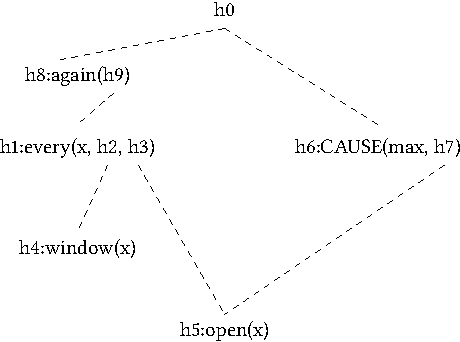
\includegraphics{Figures/mrs-max-wieder-alle-fenster-oeffnete-cropped.pdf}
\caption{Dominance graph for \emph{Max wieder alle Fenster öffnete} `that Max opened all the
  windows again'\label{Abbildung-Max-wieder-alle-Fenster-oeffnete}}
\end{figure}%
Figure~\vref{Abbildung-Max-alle-Fenster-wieder-oeffnete} shows the graph for (\ref{ex-alle-wieder})
-- repeated here as (\mex{1}):\todostefan{Skopus hinzufügen?}
\ea
\label{ex-alle-wieder-zwei}
\gll dass Max alle Fenster wieder öffnete\\
	 that Max all windows again opened\\
\z
\begin{figure}
\centering
%% \begin{tabular}{@{}ccc@{}}
%%                                & \mybox[h0]{h0}                & \\[8ex]
%% \mybox[h1]{h1:every(x, \mybox[h2]{h2}, \mybox[h3]{h3})}      &                              &                               \mybox[h6]{h6:CAUSE(max, \mybox[h7]{h7})}\\[4ex]
%%                                                               \multicolumn{2}{c}{\hspace{3em}\mybox[h8]{h8:again(\mybox[h9]{h9})}}\\[4ex]
%% \mybox[h4]{h4:window(x)}           &          & \\[6ex]
%%                                & \mybox[h5]{h5:open(x)}\\
%% \end{tabular}
%% \begin{tikzpicture}[overlay,remember picture,dashed] 
%% \draw(h0.south)--(h1.north); 
%% \draw(h0.south)--(h6.north);
%% \draw(h2.south)--(h4.north);
%% \draw(h3.south)--(h8.north);
%% \draw(h9.south)--(h5.north);
%% \draw(h7.south)--(h5.north);
%% \end{tikzpicture}
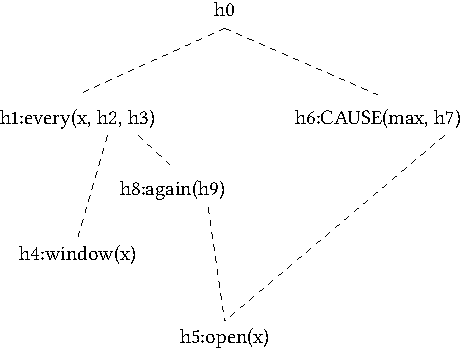
\includegraphics{Figures/mrs-max-alle-fenster-wieder-oeffnete-cropped.pdf}
\caption{Dominance graph for \emph{Max alle Fenster wieder öffnete} `that Max opened all the
  windows again'\label{Abbildung-Max-alle-Fenster-wieder-oeffnete}}
\end{figure}%
To derive these dominance graphs from the ones without \emph{wieder} `again', all one has to do is add the expression h8:again(h9)
and the dominance requirements that demand that $h9$ dominates quantifiers occurring to the right of \emph{wieder} and that it
is dominated by quantifiers to the left of \emph{wieder}.

It is therefore unproblematic to derive the relevant readings for modification by \emph{wieder}
without empty elements for CAUSE and BECOME. The meaning of the word \emph{öffnen} is decomposed in a similar way but the
decomposed meaning is assigned to a single element, the verb. By underspecification of the scopal
relations in the lexicon, the relevant readings can then be derived. 


%% Shravan sagt nee, wahrscheinlich nicht. 24.06.2008
%% Unterspezifikation ist auch psycholinguistisch plausibler als die explizite Ableitung aller Skopus:
%% Es ist unwahrscheinlich, dass Menschen für normale Sätze jeweils Tausende Repräsentationen
%% verwenden, die sich nur in verschiedenen Skopus unterscheiden. Stattdessen lassen sie wahrscheinlich
%% die Bedeutung weitestgehend unterspezifiziert und lösen sie dann bei ausreichendem Kontextwissen
%% weiter auf.

\section{Evidence for empty elements}
\label{Abschnitt-Evidenz-leere-Elemente}

As previously discussed, grammarians agree that both linguists and speakers notice when there is a constituent missing from a
string of words. For cases where it can be shown that analyses with or without traces are indistinguishable empirically,
then one can assume empty elements. Nevertheless, the learnability argument put forward by
Construction Grammarians has some validity: if one assumes that there is no or little innate linguistic knowledge, then it is not possible to motivate empty elements
with data from other languages. This means that just because Basque\il{Basque} shows object agreement\is{agreement!object},
this does not mean that one can assume an empty head for object agreement
(AgrO\is{category!functional!AgrO}) in a grammar of German as
for instance \citet{Stechow96a} and \citet{Meinunger2000a} do. Since there is no object agreement in German, there
would be no way for the child to learn the fact that there is an AgrO head. Knowledge about AgrO
must therefore be innate. Since the assumption of innate linguistic knowledge is controversial (see
Chapter~\ref{chap-innateness}), any theory that uses cross"=linguistic data to motivate the use of empty elements is on shaky ground.

Cross"=linguistic considerations can only be drawn upon if there are no empirical differences between multiple alternative
analyses compatible and motivated by the language under consideration. In this case, one should follow Occam's Razor and choose the analysis which is compatible with analyses of
other languages (see \citealp{MuellerCoreGram} and Chapter~\ref{sec-develop-theories-coregram}).
\is{empty element|)}


\section{Transformations, lexical rules, and empty elements}
\label{Abschnitt-leere-Elemente-LRs-Transformations}

In\is{empty element|(}\is{lexical rule|(}\is{transformation|(} the discussion of the passive\is{passive} in the framework of TAG, it became clear that lexical rules
correspond to particular transformations, namely those which have some relation to a lexical item (lexically governed transformations, \citealp{Dowty78a}; 
for the discussion of transformations and lexical rules, see \citew{Bresnan78a} and \citew{BK82a}). In the respective variants of TAG\indextag, lexical rules establish a relation
between a lexical item for an active tree with a lexical item of a passive tree. Both the active and passive tree can be extended by adjunction.

In theories such as Categorial Grammar\indexcg, the situation is similar: since the direction in which a functor expects to find its argument is fixed
for languages such as English, the lexical item stands for an entire tree. Only the attachment of
adjuncts is not yet specified in lexical items. The positions in the
tree where the adjuncts can occur depend on the properties of the adjuncts. In Section~\ref{Abschnitt-CG-lokale-Umstellung},
we have seen suggestions for treatments of languages with free constituent order. If the direction of combination is not fixed in the lexicon, then the lexical item
can occur in a number of trees. If we compare lexical rules that can be applied to this kind of lexical items with transformations, we see that lexical rules create relations
between different sets of trees.

In \hpsg analyses\indexhpsg, this works in a similar way: lexical rules relate lexical items with differing valence properties to each other. In HPSG grammars of English\il{English},
there is normally a schema that licenses a VP containing the verb and all its complements as well as a schema that connects the subject to the VP 
\citep[\page 39]{ps2}. In the lexical items for finite verbs, it is already determined what the tree will look like in the end. As in Categorial Grammar, adjuncts in HPSG can
be combined with various intermediate projections. Depending on the dominance schemata used in a particular grammar, the lexical item will determine the constituent structure
in which it can occur or allow for multiple structures. In the grammar of German proposed in Chapter~\ref{Kapitel-HPSG}, it is possible to analyze six different sequences with a lexical
item for a ditransitive verb, that is, the lexical item can -- putting adjuncts aside -- occur in six different structures with verb"=final order. Two sequences can be analyzed
with the passive lexical item, which only has two arguments.
As in Categorial Grammar, sets of licensed structures are related to other sets of licensed structures. In HPSG theorizing and also in Construction Grammar, there have been
attempts to replace lexical rules with other mechanisms since their ``status is dubious and their interaction with other analyses is controversial''
\citep*[\page 19]{BMS2001a}. \citet{BMS2001a} propose an analysis for extraction
that, rather than connecting lexical items with differing valence lists, establishes a relation between a subset of a particular list in a lexical item and another
list in the same lexical item. The results of the two alternative analyses are shown in (\mex{1})
and (\mex{2}), respectively:
\eal
\ex \ms{ subcat & \sliste{ NP[\type{nom}], NP[\type{acc}] }\\
         slash  & \eliste\\
       }
\ex \ms{ subcat & \sliste{ NP[\type{nom}] }\\
         slash  & \sliste{ NP[\type{acc}] }\\
       }
\zl
\addlines
In (\mex{0}), (\mex{0}a) is the basic entry and (\mex{0}b) is related to (\mex{0}a) via a lexical
rule. The alternative analysis would only involve specifying the appropriate value
of the \textsc{arg-st} feature\footnote{
\argst stands for \emph{Argument Structure}. The value of \argst is a list containing all the arguments
of a head. For more on \argst, see Section~\ref{Abschnitt-Arg-St}.
}\isfeat{arg-st} and the \subcat and \slashv is then derived from the \argstv using the relevant constraints.
(\mex{1}) shows two of the licensed lexical items.
\eal
\ex \ms{ arg-st & \sliste{ NP[\type{nom}], NP[\type{acc}] }\\
         subcat & \sliste{ NP[\type{nom}], NP[\type{acc}] }\\
         slash  & \eliste\\
       }
\ex \ms{ arg-st & \sliste{ NP[\type{nom}], NP[\type{acc}] }\\
         subcat & \sliste{ NP[\type{nom}] }\\
         slash  & \sliste{ NP[\type{acc}] }\\
       }
\zl
If we want to eliminate lexical rules entirely in this way, then we would require an additional feature for each change.\footnote{
Alternatively, one could assume a very complex relation that connects \argst and \subcat. But this would then have to deliver
the result of an interaction of a number of phenomena and the interaction of these phenomena would not be captured in a transparent way.%
} Since there are many interacting valence"=changing processes, things only work out with the stipulation of a large number of auxiliary
features. The consequences of assuming such analyses have been discussed in detail in
\citew[Section~7.5.2.2]{MuellerLehrbuch1}. The problems that arise are parallel for
inheritance"=based approaches for argument structure"=changing processes: they also require
auxiliary features since it is not possible to model embedding and multiple changes of valence information with inheritance. See Section~\ref{Abschnitt-Passiv-CxG}.

Furthermore, the claim that the status of lexical rules is dubious must be rejected: there are worked"=out formalizations of lexical rules \citep{Meurers2001a,CB92a,LC99a}
and their interaction with other analyses is not controversial. Most HPSG implementations make use of lexical rules and the interaction of a number of rules and
constraints can be easily verified by experiments with implemented fragments.

\citet{Jackendoff75a} presents two possible conceptions of lexical rules: in one variant, the lexicon contains all words in a given language and there
are just redundancy rules saying something about how certain properties of lexical entries behave with regard to properties of other lexical entries. For example,  \stem{les} `read-' and \emph{lesbar}
`readable' would both have equal status in the lexicon. In the other way of thinking of lexical
rules, there are a few basic lexical entries and the others are derived
from these using lexical rules. The stem  \stem{les} `read-' would be the basic entry and \emph{lesbar} would be derived from it.
In HPSG, the second of the two variants is more often assumed. This is equivalent to the assumption of unary rules. In Figure~\ref{Abbildung-Verbstellung-HPSG} on
page~\pageref{Abbildung-Verbstellung-HPSG}, this has been shown accordingly: the verb \emph{kennt}
`knows' is mapped by a lexical rule to a verb that selects the projection of an
empty verbal head. With this conception of lexical rules, it is possible to remove lexical rules from the grammar by assuming binary"=branching structures with an
empty head rather than unary rules. For example, in HPSG analyses of resultative constructions\is{resultative construction}\is{construction!resultative|(}
such as (\mex{1}), lexical rules have been proposed (\citealp{Verspoor97a}; \citealp{Wechsler97a}; \citealp{WN2001a}; \citealp[Chapter~5]{Mueller2002b}).
\ea
\gll [dass] Peter den Teich leer fischt\\
	 \spacebr{}that Peter the pond empty fishes\\
\glt `that Peter fishes the pond empty'
\z
In my own analysis, a lexical rule connects a verb used intransitively to a verb that selects an accusative object and a predicate.
Figure~\vref{Abbildung-Resultativ-LR} shows the corresponding tree.
\begin{figure}
\centering
\begin{forest}
sm edges
[V{[\subcat \eliste]}
	[NP{[\type{nom}]}
		[Peter;Peter]]
	[V{[\subcat \sliste{ NP[\type{nom}] }]}
		[NP{[\type{acc}]}
			[den Teich;the pond, roof]]
		[V{[\subcat \sliste{ NP[\type{nom}], NP[\type{acc}] } ]}
			[Adj
				[leer;empty]]
			[V{[\subcat \sliste{ NP[\type{nom}], NP[\type{acc}], Adj } ]}
				[V{[\subcat \sliste{ NP[\type{nom}]} ]}
					[fischt;fishes]]]]]]
\end{forest}
\caption{\label{Abbildung-Resultativ-LR}Analysis of the resultative construction with a lexical rule}
\end{figure}%
If we consider what (\mex{0}) means, then we notice that the fishing act causes the pond to become empty.
This causation is not contained in any of the basic lexical items for the words in (\mex{0}).
In order for this information to be present in the semantic representation of the entire expression, it has
to be added by means of a lexical rule. The lexical rule says: if a verb is used with an additional predicate and accusative
object, then the entire construction has a causative meaning.

Figure~\vref{Abbildung-Resultativ-leer} shows how a lexical rule can be replaced by an empty head.
\begin{figure}
\centering
\begin{sideways}
%\scalebox{0.9}{%
\begin{forest}
sm edges
[V{[\subcat \eliste]}
	[{NP[\type{nom}]}
		[Peter;Peter]]
	[{V[\subcat \sliste{ NP[\type{nom}] }]}
		[{NP[\type{acc}]}
			[den Teich;the pond,roof]]
		[{V[\subcat \sliste{ NP{[\type{nom}]}, NP{[\type{acc}]} }]}
			[Adj
				[leer;empty]]
			[{[\subcat \sliste{ NP{[\type{nom}]}, NP{[\type{acc}]}, Adj }]}
				[{V[\subcat \sliste{ NP{[\type{nom}]} }]}
					[fischt;fishes]]
				[{V[\subcat \sliste{ NP{[\type{nom}]}, NP{[\type{acc}]}, Adj, V{[\subcat \sliste{ NP{[\type{nom}]} }]} }]}
					[\trace]]]]]]
\end{forest}
%}
\end{sideways}
\caption{\label{Abbildung-Resultativ-leer}Analysis of the resultative construction with an empty head}
\end{figure}%
The empty head requires the intransitive verb and additionally an adjective, an accusative object and a subject.
The subject of \emph{fischt} `fishes' must of course be identical to the subject that is selected by the combination
of \emph{fischt} and the empty head. This is not shown in the figure.
It is possible, however, to establish this identity (see \citealp{HN94a}). The causative semantics is contributed by
the empty head in this analysis. The trick that is being implemented here is exactly what was done in Section~\ref{Abschnitt-Eleminierung-leerer-Elemente},
just in the opposite direction: in the previous section, binary"=branching structures with an empty daughter were replaced by unary"=branching structures.
In this section, we have replaced unary"=branching structures with binary"=branching structures with an empty daughter.\footnote{
	Here, we are discussing lexical rules, but this transformation trick can also be applied to
        other unary rules. Semanticists often use such rules for type shifting\is{type raising}. For
        example, a rule that turns a referential NP such as \emph{a trickster} in (i.a) into a
        predicative one (i.b) \citep{Partee87a-u}.
\eal
\ex A trickster laughs.
\ex He is a trickster.
\zl
These changes can be achieved by a unary rule that is applied to an NP or with a special empty head that takes an NP as its argument. In current Minimalist\indexmp approaches,
empty heads are used \citep[\page 370]{Ramchand2005a}, in Categorial Grammar\indexcg and HPSG\indexhpsg unary"=branching rules are more common (\citealp[\page
    91--92]{Flickinger2008a}; \citealp{MuellerPredication,MuellerCopula}).
}\is{empty element|)}\is{lexical rule|)}\is{transformation|)}\is{construction!resultative|)}

\largerpage
We have therefore seen that certain transformations can be replaced by lexical rules and also that
lexical rules can be replaced by empty heads. 
The following chapter
%will deal with the question of whether meaning is contributed by lexical heads or rather holistically by phrasal configurations.
deals with the question of whether phenomena like extraction, scrambling, and passive should be
described with the same tool as in GB/Minimalism or with different tools as in LFG and HPSG.



%      <!-- Local IspellDict: en_US-w_accents -->

%% -*- coding:utf-8 -*-
\chapter{Extraction, scrambling, and passive: one or several descriptive devices?}
\label{chap-scrambling-extraction-passive}

An anonymous reviewer suggested discussing one issue in which transformational theories differ from
theories like LFG and HPSG. The reviewer claimed that Transformational Grammars use just one tool
for the description of active/passive alternations, scrambling, and extraction, while theories like
LFG and HPSG use different techniques for all three phenomena. If this claim were correct and if
the analyses made correct predictions, the respective GB/Minimalism theories would be better
than their competitors, since the general aim in science
is to develop theories that need a minimal set of assumptions. I already commented on the analysis of
passive in GB in Section~\ref{sec-passive-gb}, but I want to extend this discussion here and include
a Minimalist analysis and one from Dependency Grammar. 

The task of any passive analysis is to explain the difference in argument realization in examples
like (\mex{1}):
\eal
\ex\label{ex-she-beats-him}
She beats him.
\ex\label{ex-he-was-beaten}
He was beaten.
\zl
In these examples about chess, the accusative object of \emph{beat} is realized as the nominative
in (\mex{0}b). In addition, it can be observed that the position of the elements is different: while
\emph{him} is realized postverbally in object position in (\mex{0}a), it is realized preverbally in
(\mex{0}b). In GB this is explained by a movement analysis. It is assumed that the object does not
get case in passive constructions and hence has to move into the subject position where case is
assigned by the finite verb. This analysis is also assumed in Minimalist work as in
David Adger's textbook \citeyearpar{Adger2003a}, for instance. Figure~\vref{fig-passive-mp} shows his analysis
of (\mex{1}):
\ea
Jason was killed.
\z
\begin{figure}
\centerfit{
\begin{forest}
for tree={fit=rectangle}
[TP
  [Jason]
  [{\tbar[\st{\textit{u}N*}]}
     [{T[past,\st{nom}]}
       [be{[Pass,\st{\textit{u}Infl}:past*]}]
       [{T[past]}]]
     [PassP
       [\phonliste{be}]
       [\vP
         [\textit{v}
           [\textit{kill}]
           [{\textit{v}[\st{\textit{u}Infl}:Pass]}]]
         [VP
           [\phonliste{kill}]
           [\phonliste{Jason}]]]]]]
]
\end{forest}
}
\caption{\label{fig-passive-mp}Adger's Minimalist movement-based analysis of the passive (p.\,231)}
\end{figure}%
TP stands for Tense Phrase and corresponds to the IP that was discussed in
Chapter~\ref{chap-GB}. PassP is a functional head for passives\is{category!functional!PassP}. \vP\is{category!functional!v@\textit{v}} is
a special category for the analysis of verb phrases that was originally introduced for the analysis
of ditransitives \citep{Larson88a}
%; \citealp[\page 315]{Chomsky95a}) auch für transitive Verben
and VP is the normal VP that consists of verb and object. In Adger's analysis, the
verb \emph{kill} moves from the verb position in VP to the head position of \textit{v}, the
passive auxiliary \emph{be} moves from the head position of PassP to the head position of the Tense
Phrase. Features like Infl are `checked' in combination with such movements. The exact implementation
of these checking and valuing operations does not matter here. What is important is that
\emph{Jason} moves from the object position to a position that was formerly known as the specifier
position of T (see Footnote~\ref{fn-Chomsky-on-Specifiers} on
page~\pageref{fn-Chomsky-on-Specifiers} on the notion of specifier). All these analyses assume that
the participle cannot assign accusative to its object and that the object has to move to another
position to get case or check features.
How exactly one can formally represents the fact that the participle cannot assign case is hardly ever made explicit in the GB literature.\todostefan{Baker, Johnson, Roberts 1989 sagen, dass der akkusativ dem pro externen Argument zugewiesen wird}
The following is a list of statements that can be found in the literature:
\eal
\ex We shall assume that a passivized verb loses the ability to assign structural ACCUSATIVE case to
its complement. \citep[\page 183]{Haegeman94a-u}

\ex das Objekt des Aktivsatzes wird zum Subjekt des Passivsatzes, weil die passivische Verbform
keinen Akkusativ"=Kasus regieren kann (Akk"=Kasus"=Absorption). \citep[\page 172]{Lohnstein2014a} 
\zl
In addition, it is sometimes said that the external theta role is absorbed by the verb morphology
(\citealp{Jaeggli86a}; 
%\citealp[]{Roberts87a}; 
\citealp[\page 183]{Haegeman94a-u}). Now, what would it entail if we made this explicit? There is some
lexical item for verbs like \emph{beat}. The active form has the ability to assign accusative to its
object, but the passive form does not. Since this is a property that is shared by all transitive
verbs (by definition of the term transitive verb), this is some regularity that has to be
captured. One way to capture this is the assumption of a special passive morpheme that suppresses
the agent and changes something in the case specification of the stem it attaches too. How this
works in detail was never made explicit.
Let us compare this morpheme"=based analysis with lexical rule"=based analyses: as was explained in
Section~\ref{Abschnitt-leere-Elemente-LRs-Transformations}, empty heads can be used instead of
lexical rules in those cases in which the phonological form of the input and the output do not
differ. So for example, lexical rules that license additional arguments as in
resultative constructions, for instance, can be replaced by an empty head. However, as was explained in Section~\ref{Abschnitt-HPSG-Passiv}, lexical 
rules are also used to model morphology. This is also true for Construction Grammar\indexcxg (see
Gert Booij's work on Construction Morphology \citeyearpar{Booij2010a}, which is in many ways similar to Riehemann's work in
HPSG \citeyearpar{Riehemann93a,Riehemann98a}). In the case of the passive lexical rule, the participle
morphology is combined with the stem and the subject is suppressed in the corresponding valence
list. This is exactly what is described in the GB/MP literature. The respective lexical rule for the
analysis of \emph{ge-lieb-t} `loved' is depicted in Figure~\vref{fig-morpheme-vs-lexical-rule} to
the left.
\begin{figure}
\hfill
\begin{forest}
[{[ \phon \phonliste{ ge } $\oplus$ \ibox{1} $\oplus$ \phonliste{ t } ]}
   [ {[ \phon \ibox{1} ]}   ]]
\end{forest}
\hfill
\begin{forest}
[V
  [V-Aff [ge]]
  [V-Stem]
  [V-Aff [t]]]
\end{forest}
\hfill\mbox{}
\caption{\label{fig-morpheme-vs-lexical-rule}Lexical rule"=based/constructionist
  vs.\ morpheme"=based analysis}
\end{figure}%
The morpheme"=based analysis is shown to the right. To keep things simple, I assume a flat analysis,
but those who insist on binary branching structures would have to come up with a way of deciding
whether the \prefix{ge} or the \suffix{t} is combined first with the stem and in which way selection
and percolation of features takes place. Independent of how morphology is done, the fact  that the inflected form (the top node in both figures) has different properties than the
verb stem has to be represented somehow. In the morpheme"=based world, the morpheme is responsible for suppressing the agent and
changing the case assignment properties, in the lexical rule/construction world this is done by the
respective lexical rule. There is no difference in terms of needed tools and necessary stipulations.

The situation in Minimalist theories is a little bit different. For instance, \citep[\page 229,
  231]{Adger2003a} writes the following:
\begin{quote}
Passives are akin to unaccusatives, in that they do not assign accusative case to their object,
and they do not appear to have a thematic subject. [\ldots] Moreover, the idea that the function of
this auxiliary is to select an unaccusative little \vP simultaneously explains the lack of
accusative case and the lack of a thematic subject. \citep[\page 229, 231]{Adger2003a}  
\end{quote}
So this is an explicit statement. The relation between a stem and a passive participle form that was
assumed in GB analyses is now a verb stem that is combined with two different versions of
\littlev. Which \textit{v} is chosen is determined by the governing head, a functional
Perf\is{category!functional!Perf} head or a Pass\is{category!functional!Pass} head. This can be
depicted as in Figure~\vref{fig-Pass-vs-Perf-and-little-v}.
\begin{figure}
\hfill
\begin{forest}
[\vP
     [DP]
     [\littlevbar
       [\textit{v}{[\st{\textit{u}D}]}]
       [VP
         [\textit{kill} {[V, \st{\textit{u}D}]}]
         [DP ]]]]
\end{forest}
\hfill
\begin{forest}
[\vP
       [\textit{v}]
       [VP
         [\textit{kill} {[V, \st{\textit{u}D}]}]
         [DP ]]]
\end{forest}
\hfill\mbox{}
\caption{\label{fig-Pass-vs-Perf-and-little-v}Analysis of the passive and the perfect and the
  passive in a Minimalist theory involving two different versions of \littlev}
\end{figure}%
When \emph{kill} is used in the perfect or the passive, it is spelled out as \emph{killed}. If it
is used in the active with a 3rd person singular subject it is spelled out as \emph{kills}. This can
be compared with a lexical analysis, for instance the one assumed in HPSG. The analysis
is shown in Figure~\vref{fig-LR-passive-HPSG}.
\begin{figure}
\hfill
\begin{forest}
[V\feattab{\spr   \sliste{ \ibox{1} },\\
           \comps \sliste{ \ibox{2} },\\
           \argst \sliste{ \ibox{1} NP[\str], \ibox{2} NP[\str] }}
 [V\feattab{
           \argst \sliste{ \ibox{1} NP[\str], \ibox{2} NP[\str] }}]]
\end{forest}
\hfill
\begin{forest}
[V\feattab{\spr   \sliste{ \ibox{2} },\\
           \comps \sliste{ },\\
           \argst \sliste{ \ibox{2} NP[\str] }}
 [V\feattab{
           \argst \sliste{ \ibox{1} NP[\str], \ibox{2} NP[\str] }}]]
\end{forest}
\hfill\mbox{}
\caption{\label{fig-LR-passive-HPSG}Lexical rule"=based analysis of the perfect and the passive in HPSG}
\end{figure}%
The left figure shows a lexical item that is licensed by a lexical rule that is applied to the stem
\stem{kill}. The stem has two elements in its argument structure list and for the active forms the
complete argument structure list is shared between the licensed lexical item and the stem. The first
element of the \argstl is mapped to \spr and the other elements to \comps (in English). Passive is
depicted in the right figure: the first element of the \argst with structural case is suppressed and
since the element that was the second element in the \argstl of the stem \iboxb{2} is now the first element,
this item is mapped to \spr. See Section~\ref{sec-hpsg-passive} for passive in HPSG and Section~\ref{Abschnitt-Arg-St} for comments on
\argst and the differences between German and English\il{English}. 

The discussion of Figures~\ref{fig-Pass-vs-Perf-and-little-v} and~\ref{fig-LR-passive-HPSG} are
a further illustration of a point made in Section~\ref{Abschnitt-leere-Elemente-LRs-Transformations}:
lexical rules can be replaced by empty heads and vice versa. While HPSG says there are stems that
are related to inflected forms and corresponding to the inflection the arguments are realized in a
certain way, Minimalist theories assume two variants of \littlev that differ in their selection of
arguments. Now, the question is: are there empirical differences between the two approaches? I think
there are differences if one considers the question of language acquisition. What children can
acquire from data is that there are various inflected forms and that they are related somehow. What
remains questionable is whether they really would be able to detect empty little \textit{v}s. One
could claim of course that children operate with chunks of structures such as the ones in
Figure~\ref{fig-Pass-vs-Perf-and-little-v}. But then a verb would be just a chunk consisting of
\littlev and V and having some open slots. This would be indistinguishable from what the HPSG
analysis assumes.


As far as the ``lexical rules as additional tool'' aspect is concerned, the discussion is closed, but
note that the standard GB/Minimalism analyses differ in another way from LFG and HPSG analyses,
since they assume that passive has something to do with movement, that is, they assume that the same mechanisms
are used that are used for nonlocal dependencies.\footnote{
  There is another option in Minimalist theories. Since Agree\is{Agree} can check features
  nonlocally, T can assign nominative to an embedded element. So, in principle the object may get
  nominative in the VP without moving to T. However, \citet[\page 368]{Adger2003a} assumes that German has a
  strong EPP feature on T, so that the underlying object has to move to the specifier of T. This is
  basically the old GB analysis of passive in German with all its conceptual problems and disadvantages.
}
This works for languages like English in which
the object has to be realized in postverbal position in the active and in preverbal position in the
passive, but it fails for languages like German in which the order of constituents is more free.
\citet[Section~4.4.3]{Lenerz77} discussed the examples in (\ref{ex-passive-German-no-movement}) on
page~\pageref{ex-passive-German-no-movement} -- which are repeated here as
(\ref{ex-passive-German-no-movement-two}) for convenience:
\eal
\label{ex-passive-German-no-movement-two}
\ex 
\gll weil das Mädchen dem Jungen den Ball schenkt\\
     because the girl the.\dat{} boy the.\acc{} Ball gives\\
\glt `because the girl gives the ball to the boy'
\ex 
\gll weil dem Jungen der Ball geschenkt wurde\\
     because the.\dat{} boy the.\nom{} ball given was\\
\ex 
\gll weil der Ball dem Jungen geschenkt wurde\\
     because the.\nom{} ball the.\dat{} boy given was\\
\glt `because the ball was given to the boy'
\zl
While both orders in (\mex{0}b) and (\mex{0}c) are possible, the one with dative--nominative order
in (\mex{0}b) is the unmarked one. There is a strong linearization preference in German demanding that
animate NPs be serialized before inanimate ones \citep[\page 46]{Hoberg81a}. This linearization rule is
unaffected by passivization. 
Theories that assume that passive is movement either have to
assume that the passive of (\mex{0}a) is (\mex{0}c) and (\mex{0}b) is derived from (\mex{0}c) by a
further reordering operation (which would be implausible since usually one assumes that more marked
constructions require more transformations), or they would have to come up with other
explanations for the fact that the subject of the passive sentence has the same position as the
object in active sentences. As was already explained in Section~\ref{sec-passive-gb}, one such explanation is to
assume an empty expletive subject that is placed in the position where nominative is assigned and
to somehow connect this expletive element to the subject in object position. While this somehow
works, it should be clear that the price for rescuing a movement"=based analysis of passive is rather
high: one has to assume an empty expletive element, that is, something that neither has a form nor a
meaning. The existence of such an object could not be inferred from the input unless it is assumed
that the structures in which it is assumed are given. Thus, a rather rich UG\indexug would have to be
assumed. 

The question one needs to ask here is: why does the movement"=based analysis have these problems and why
does the valence"=based analysis not have them? The cause of the problem is that the analysis
of the passive mixes two things: the fact that SVO languages like English encode subjecthood
positionally, and the fact that the subject is suppressed in passives. If these two things are
separated the problem disappears. The fact that the object of the active sentence in (\ref{ex-she-beats-him}) is
realized as the subject in (\ref{ex-he-was-beaten}) is explained by the assumption that the first NP on the
argument structure list with structural case is realized as subject and mapped to the respective valence feature: \spr in
English. Such mappings can be language specific (see Section~\ref{Abschnitt-Arg-St} and
\citew{MuellerGermanic} where I discuss Icelandic\il{Icelandic}, which is an SVO language with
subjects with lexical case).

In what follows, I discuss another set of examples that are sometimes seen as evidence for a
movement"=based analysis. The examples in (\mex{1}) are instances of the so"=called remote passive\is{passive!remote}
\citep[\page 175--176]{Hoehle78a}.\footnote{
  See \citew[Section~3.1.4.1]{Mueller2002b} and \citew{Wurmbrand2003a} for corpus examples.
}
\eal
\ex\iw{versuchen|(}
\gll daß er auch von mir zu überreden versucht wurde\footnotemark\\
     that he.\nom{} also from me to persuade tried got\\
\footnotetext{
        \citew*[\page 212]{Oppenrieder91a}\ia{Oppenrieder}.%
}
\glt `that an attempt to persuade him was also made by me'
\ex 
\gll weil    der Wagen oft zu reparieren versucht wurde\\
     because the car.\nom{}   often to repair   tried     was\\
\glt `because many attempts were made to repair the car'\label{bsp-zu-reparieren-versucht-wurde}
%,
\zl
What is interesting about these examples is that the subject is the underlying object of a deeply
embedded verb. This seems to suggest that the object is extracted out of the verb phrase. So the
analysis of (\mex{0}b) would be (\mex{1}):
\ea
\gll weil    [\sub{IP} der Wagen$_i$ [\sub{VP} oft   [\sub{VP} [\sub{VP} [\sub{VP} \_$_i$ zu reparieren] versucht] wurde]\\
     because {}        the car.\nom{} {}        often {}        {}        {}        {}    to repair       tried     was\\
\z
While this is a straight-forward explanation of the fact that
(\ref{bsp-zu-reparieren-versucht-wurde}) is grammatical, another explanation is possible as well. In
the HPSG analysis of German (and Dutch\il{Dutch}) it is assumed that verbs like those in
(\ref{bsp-zu-reparieren-versucht-wurde}) form a verbal complex, that is, \emph{zu reparieren
  versucht wurde} `to repair tried was' forms one unit. When two or more verbs form a complex, the
highest verb attracts the arguments from the verb it embeds \citep{HN89a,HN94a,BvN98}. A verb like
\emph{versuchen} `to try'
selects a subject, an infinitive with \emph{zu} `to' and all complements that are selected by this
infinitive. In the analysis of (\mex{1}), \emph{versuchen} `to try' selects for its subject, the
object of \emph{reparieren} `to repair' and for the verb \emph{zu reparieren} `to repair'.
\ea
\gll weil er den Wagen zu reparieren versuchen will\\
     because he.\nom{} the.\acc{} car to repair try wants\\
\glt `because he wants to try to repair the car'
\z
Now if the passive lexical rule applies to \stem{versuch}, it suppresses the first argument of
\stem{versuch} with structural case, which is the subject of \stem{versuch}. The next argument of
\stem{versuch} is the object of \emph{zu reparieren}. Since this element is the first NP with
structural case, it gets nominative as in (\ref{bsp-zu-reparieren-versucht-wurde}). So, this shows
that there is an analysis of the remote passive that does not rely on movement. Since
movement"=based analyses were shown to be problematic and since there are no data that cannot be
explained without movement, analyses without movement have to be preferred.

This leaves us with movement"=based accounts of local reordering (scrambling). The reviewer
suggested that scrambling, passive, and nonlocal extraction may be analyzed with the same
mechanism. It was long thought that scope facts made the assumption of movement"=based analyses of
scrambling necessary, but it was pointed out by \citew[\page 146]{Kiss2001a} and
\citew[Section~2.6]{Fanselow2001a} that the reverse is true: movement"=based accounts of scrambling
make wrong predictions with regard to available quantifier scopings. I discussed the respective
examples in Section~\ref{sec-GB-lokale-Umstellung} already and will not repeat the discussion
here. The conclusion that has to be drawn from this is that passive, scrambling, and long distance
extraction are three different phenomena that should be treated differently. The solution for the
analysis of the passive that is adopted in HPSG is based on an analysis by \citet{Haider86}, who
worked within the GB framework. The ``scrambling-as-base generation'' approach to local reordering
that was used in HPSG right from the beginning \citep{Gunji86a} is also adopted by some practitioners
of GB/Minimalism, \eg \citet{Fanselow2001a}.

Having discussed the analyses in GB/Minimalism, I now turn to Dependency Grammar. 
\citet{GO2009a} suggest that \emph{w}-fronting, topicalization, scrambling, extraposition,
splitting, and also the remote passive should be analyzed by what they call
\emph{rising}\is{rising}. The concept was already explained in Section~\ref{sec-nld-dg}. The
Figures~\ref{fig-die-idee-wird-jeder-verstehen-dg-rising}
and~\ref{fig-gestern-hat-sich-der-spieler-verletzt-dg-rising} show examples for the fronting and the scrambling of an object.
\begin{figure}
\centering
\begin{forest}
dg edges
[V
  [N, edge=dashed 
    [Det [die;the] ]
    [Idee;idea]] 
  [wird;will] 
  [N [jeder;everybody] ]
  [V$_g$ [verstehen;understand]]]
\end{forest}
\caption{\label{fig-die-idee-wird-jeder-verstehen-dg-rising}Analysis of \emph{Die Idee wird jeder
    verstehen.} `Everybody will understand the idea.' involving rising}
\end{figure}%%
\begin{figure}
\centering
\begin{forest}
dg edges
[V
  [Adv [Gestern;yesterday] ]
  [hat;has] 
  [N, edge=dashed [sich;himself] ]
  [N
    [Det [der;the]]
    [Spieler;player]]
  [V$_g$ [verletzt;injured]]]
\end{forest}
\caption{\label{fig-gestern-hat-sich-der-spieler-verletzt-dg-rising}Analysis of \emph{Gestern hat
    sich der Spieler verletzt.} `Yesterday, the player injured himself.' involving rising of the object of the main
  verb \emph{verletzt} `injured'}
\end{figure}%%
Groß and Osborne assume that the object depends on the main verb in sentences with auxiliary verbs,
while the subject depends on the auxiliary. Therefore, the object \emph{die Idee} `the idea' and
the object \emph{sich} `himself' have to rise to the next higher verb in order to keep the
structures projective\is{projectivity}.
Figure~\vref{fig-dass-der-wagen-zu-reparieren-versucht-wurde-dg-rising} shows the analysis of the
remote passive.
\begin{figure}
\centering
\begin{forest}
dg edges
[Subjunction
  [dass;that]
  [V
    [N, edge=dashed
      [Det [der;the]]
      [Wagen;car]]
    [V
      [V$_g$ [zu reparieren;to repair]]
      [versucht;tried]]
    [wurde;was]]]
\end{forest}
\caption{\label{fig-dass-der-wagen-zu-reparieren-versucht-wurde-dg-rising}Analysis of the remote
  passive \emph{dass der Wagen zu reparieren versucht wurde} `that it was tried to repair the car' involving rising}
\end{figure}%%
The object of \emph{zu reparieren} `to repair' rises to the auxiliary \emph{wurde} `was'.

Groß and Osborne use the same mechanism for all these phenomena, but it should be clear that there
have to be differences in the exact implementation. Groß and Osborne say that English does not have
scrambling, while German does. If this is to be captured, there must be a way to distinguish the two
phenomena, since if this were not possible, one would predict that English has scrambling as well,
since both German and English allow long distance fronting. \citet[\page 58]{GO2009a} assume
that object nouns that rise must take the nominative. But if the kind of rising that they assume
for remote passives is identical to the one that they assume for scrambling, they would predict that
\emph{den Wagen} gets nominative in (\mex{1}) as well:
\ea
\gll dass den Wagen niemand repariert hat\\
     that the.\acc{} car nobody.\nom{} repaired has\\
\glt `that nobody repaired the car'
\z
Since \emph{den Wagen} `the car' and \emph{repariert} `repaired' are not adjacent, \emph{den Wagen} has to rise to the
next higher head in order to allow for a projective realization of elements. So in order to assign
case properly, one has to take into account the arguments that are governed by the head to which a
certain element rises. Since the auxiliary \emph{hat} `has' already governs a nominative, the NP \emph{den
  Wagen} has to be realized in the accusative. An analysis that assumes that both the accusative and
nominative depend on \emph{hat} `has' in (\mex{0}) is basically the verbal complex analysis
assumed in HPSG and some GB variants.

Note, however, that this does not extend to nonlocal dependencies. Case is assigned locally by verbs or
verbal complexes, but not to elements that come from far away. The long distance extraction of
NPs is more common in southern variants of German and there are only a few verbs that do not take a
nominative argument themselves. The examples below involve \emph{dünken} `to think', which governs an
accusative and a sentential object and \emph{scheinen} `to seem', which governs a dative and a
sentential object. If (\mex{1}a) is analyzed with \emph{den Wagen} rising to
\emph{dünkt}, one might expect that \emph{den Wagen} `the car' gets nominative since there is no other element
in the nominative. However, (\mex{0}b) is entirely out.

\eal
\ex[]{ 
\gll Den Wagen dünkt mich, dass er repariert.\\
     the.\acc{} car thinks me.\acc{}     that he.\nom{} repairs\\
\glt `I think that he repairs the car'
}
\ex[*]{
\gll Der Wagen dünkt mich, dass er repariert.\\
     the.\nom{} car thinks me.\acc{}     that he.\nom{} repairs\\
}
\zl

Similarly there is no agreement between the fronted element and the verb to which it attaches:
\eal
\ex[]{
\gll Mir scheint, dass die Wagen ihm gefallen.\\
     me.\dat.1\pl{} seems.3\sg{} that the cars.3\pl{} him please.3\pl{} \\
\glt `He seems to me to like the cars.'
}
%% \ex 
%% \gll Der Wagen scheint mir, dass ihm gefällt.\\
%%      the car   seems   me   that him pleases\\
\ex[]{
\gll Die Wagen scheint mir, dass ihm gefallen.\\
     the cars.3\pl{}  seem.3\sg{}     me.\dat{}   that him please.3\pl{}\\
\glt `The cars, he seems to me to like.'
}

\ex[*]{
\gll  Die Wagen scheinen mir, dass ihm gefällt.\\
      the cars.3\pl{}  seem.3\pl{}     me.\dat{}   that him pleases.3\sg{}\\
}
\ex[*]{
\gll Die Wagen scheinen mir, dass ihm gefallen.\\
     the cars.3\pl{}  seem.3\pl{}     me.\dat{}   that him please.3\pl{}\\
}
\zl
This shows that scrambling/remote passive and extraction should not be dealt with by the same mechanism or if they
are dealt with by the same mechanism one has to make sure that there are specialized variants of the
mechanism that take the differences into account. 
I think what Groß and Osborne did is simply recode the attachment relations of phrase structure
grammars. \emph{die Idee} `the idea' has some relation to \emph{wird jeder verstehen} `will
everybody understand' in Figure~\ref{fig-die-idee-wird-jeder-verstehen-dg-rising}, as it does in GB, LFG, GPSG, HPSG, and
other similar frameworks. In HPSG, \emph{die Idee} `the idea' is the filler in a filler-head configuration. The remote
passive and local reorderings of arguments of auxiliaries, modal verbs, and other verbs that behave similarly
are explained by verbal complex formation where all non-verbal arguments depend on the highest verb \citep{HN94a}.

Concluding this chapter, it can be said that local reorderings and long"=distance dependencies are two
different things that should be described with different tools (or there should be further
constraints that differ for the respective phenomena when the same tool is used). Similarly, movement"=based analyses
of the passive are problematic since passive does not necessarily imply reordering. 





%      <!-- Local IspellDict: en_US-w_accents -->

%% -*- coding:utf-8 -*-
\exewidth{(235)}


\chapter{Phrasal vs.\ lexical analyses}
\label{Abschnitt-Phrasal-Lexikalisch}

\chaptersubtitle{coauthored with Stephen Wechsler}

This section deals with a rather crucial aspect when it comes to the comparison of the theories
described in this book: valence and the question whether sentence structure, or rather syntactic
structure in general, is determined by lexical information or whether syntactic structures have an
independent existence (and meaning) and lexical items are just inserted into them. Roughly speaking,
frameworks like GB/Minimalism, LFG, CG, HPSG, and DG are lexical, while GPSG and Construction
Grammar (\citealp{Goldberg95a,Goldberg2003b,Tomasello2003a,Tomasello2006c,Croft2001a}) are
phrasal approaches. This categorization reflects tendencies, but there are non-lexical 
approaches in Minimalism (Borer's exoskeletal approach, \citeyear{Borer2003a-u}) and LFG
(\citealp{Alsina96a}; \citealp{ADT2008a,ADT2013a}) and there are lexical approaches in Construction
Grammar (Sign"=Based Construction Grammar, see Section~\ref{sec-SBCG}). The phrasal approach is
wide"=spread also in frameworks like Cognitive Grammar (\citealp{Dabrowska2001a}; \citealp[\page 169]{Langacker2009a})
 and Simpler Syntax \citep{CJ2005a,Jackendoff2008a} that could not be discussed in this book.

The question is whether the meaning of an utterance like (\mex{1}a) is contributed by the verb
\emph{give} and the structure is needed for the NPs around the verb does not contribute any meaning
or whether there is a phrasal pattern X Verb Y Z that contributes some `ditransitive meaning'
whatever this may be.\footnote{
Note that the prototypical meaning is a transfer of possession in which Y receives Z from X, but the
reverse holds in (i.b):
\eal
\ex 
\gll Er gibt ihr den Ball.\\
     he.\nom{} gives her.\dat{} the.\acc{} ball\\
\ex
\gll Er stiehlt ihr den Ball.\\
     he.\nom{} steals  her.\dat{} the.\acc{} ball\\
\glt `He steals the ball from her.'
\zllast
}
\eal
\ex Peter gives Mary the book.
\ex Peter fishes the pond empty.
\zl
Similarly, there is the question of how the constituents in (\mex{0}b) are licensed. This sentence is
interesting since it has a resultative meaning that is not part of the meaning of the verb
\emph{fish}: Peter's fishing causes the pond to become empty. Nor is this additional meaning part of
the meaning of any other item in the sentence. On the lexical account,
there is a lexical rule that licenses a lexical item that selects for \emph{Peter}, \emph{the pond},
and \emph{empty}. This lexical item also contributes the resultative meaning. On the phrasal
approach, it is assumed that there is a pattern Subj V Obj Obl. This pattern contributes the
resultative meaning, while the verb that is inserted into this pattern just contributes its
prototypical meaning, \eg the meaning that \emph{fish} would have in an
intransitive construction. I call such phrasal approaches \emph{plugging approaches}, since lexical
items are plugged into ready"=made structures that do most of the work.

In what follows I will examine these proposals in more detail and argue that the lexical approaches
to valence are the correct ones. The discussion will be based on earlier work of mine
\citep{Mueller2006d,Mueller2007d,MuellerPersian} and work that I did together with Steve Wechsler
\citep{MWArgSt,MWArgStReply}. Some of the sections in \citet{MWArgSt} started out as translations of
\citet{MuellerGTBuch2}, but the material was reorganized and refocused due to intensive discussion
with Steve Wechsler. So rather than using a translation of Section~11.11 of \citew{MuellerGTBuch2},
I use parts of \citew{MWArgSt} here and add some subsections that had to be left out of the article
due to space restrictions (Subsections~\ref{Abschnitt-Diskussion-Haugereid} and~\ref{sec-neuro-linguistics}).
Because there have been misunderstandings in the past (\eg \citew{Boas2014a}, see \citew{MWArgStReply}), a disclaimer is necessary
here. This section is not an argument against Construction Grammar. As was mentioned above
Sign"=Based Construction Grammar is a lexical variant of Construction Grammar and hence compatible
with what I believe to be correct. This section is also not against phrasal constructions in
general, since there are phenomena that seem to be best captured with phrasal constructions. These are
discussed in detail in Subsection~\ref{Abschnitt-Phrasale-Konstruktionen}. What I will argue against in
the following subsections is a special kind of phrasal construction, namely phrasal argument
structure constructions. I believe that all phenomena that have to do with valence and valence
alternations should be treated lexically.





\section{Some putative advantages of phrasal models}
\label{Abschnitt-Stoepselei}
%
%The previous section reviewed earlier
%arguments for needing lexical representations of valence.  In this section we present more detailed
%arguments specifically directed against the claim that lexical valence representations
%(i.\,e.\ predicate argument structures) can or should be replaced by what we call a plugging proposal,
%that is, a system in which a verb or other predicator is plugged into a meaningful construction.

%As noted in Section~\ref{PAS-sec} above, we believe that grammars include meaningful phrasal
%constructions.  Our purpose is not to argue against their existence, but rather to argue that they
%cannot replace lexical valence representations.  So the existence of such phrasal constructions does not bear
%on the issue at stake here.  
In this section we examine certain claims to purported advantages of phrasal versions of Construction Grammar over lexical rules.  
Then in the following section, we will turn to positive arguments for lexical rules. 

\subsection{Usage-based theories}\label{usage-based-sec}

For many practitioners of Construction Grammar, their approach to syntax is deeply rooted in the
ontological strictures of \emph{usage-based} theories of language \citep{Langacker87a-u, Goldberg95a,
Croft2001a, Tomasello2003a}.  Usage-based theorists oppose the notion of `linguistic rules conceived
of as algebraic procedures for combining symbols that do not themselves contribute to meaning'
\citep[\page 99]{Tomasello2003a}. All linguistic entities are symbolic of things in the realm of denotations;
`all have communicative significance because they all derive directly from language use' (\emph{ibid}). Although the formatives of language may be rather abstract, they can never be divorced
from their functional origin as a tool of communication.  The usage-based view of constructions is
summed up well in the following quote:
\begin{quote}
The most important point is that constructions are nothing more or less than patterns of usage,
which may therefore become relatively abstract if these patterns include many different kinds of
specific linguistic symbols.  But never are they empty rules devoid of semantic content or
communicative function. \citep[\page 100]{Tomasello2003a}
\end{quote}

\noindent 
Thus constructions are said to differ from grammatical rules in two ways: they must carry meaning;
and they reflect the actual `patterns of usage' fairly directly.

Consider first the constraint that every element of the grammar must carry meaning, which we call
the \emph{semiotic dictum}.  Do lexical or phrasal theories hew the most closely to this dictum?
Categorial Grammar, the paradigm of a lexical theory (see Chapter~\ref{chap-CG}), is a strong
contender: it consists of meaningful words, with only a few very general combinatorial rules such as
X/Y $*$ Y = X.  Given the rule-to-rule assumption, those combinatorial rules specify the meaning of the
whole as a function of the parts.  Whether such a rule counts as meaningful in itself in Tomasello's
sense is not clear.

What does seem clear is that the combinatorial rules of Construction Grammar, such as Goldberg's
Correspondence Principle for combining a verb with a construction \citeyearpar[\page 50]{Goldberg95a},
have the same status as those combinatorial rules:

%\begin{quote}
\ea
The Correspondence Principle:  each participant that is lexically profiled and expressed must be
fused with a profiled argument role of the construction.  If a verb has three profiled participant
roles, then one of them may be fused with a non-profiled argument role of a construction. \citep[\page 50]{Goldberg95a}\label{tcp}
\z
%\end{quote}
Both verbs and constructions are specified for participant roles, some of which are \emph{profiled}.
Argument profiling for verbs is `lexically determined and highly conventionalized'
\citep[\page 46]{Goldberg95a}.  Profiled argument roles of a construction are mapped to direct
grammatical functions, i.\,e., SUBJ, OBJ, or OBJ2.  By the Correspondence Principle the lexically profiled argument
roles must be direct, unless there are three of them, in which case one may be indirect.\footnote{We
  assume that the second sentence of (\ref{tcp}) provides for exceptions to the first sentence.}
With respect to the semiotic dictum, the Correspondence Principle has the same status as the
Categorial Grammar combinatorial rules: a meaningless algebraic rule that specifies the way to
combine meaningful items.   

Turning now to the lexicalist syntax we favor, some elements abide by the semiotic dictum while
others do not.  Phrase structure rules for intransitive and transitive VPs (or the respective HPSG ID schema)
do not.  Lexical valence structures clearly carry meaning since they are associated with particular
verbs.  In an English ditransitive, the first object expresses the role of `intended recipient' of
the referent of the second object.
Hence \emph{He carved her a toy} entails that he carved a toy with the intention that she receive
it.  So the lexical rule that adds a benefactive recipient argument to a verb adds meaning.  Alternatively, a phrasal ditransitive construction might
contribute that `recipient' meaning.\footnote{In Section~\ref{coordination-sec} we argue that the
  recipient should be added in the lexical argument structure, not through a phrasal construction.
  See Wechsler (\citeyear[\page 111--113]{Wechsler91a-u}; \citeyear[\page 88--89]{Wechsler95a-u}) for an
  analysis of English ditransitives with elements of both constructional and lexical approaches.  It
  is based on Kiparsky's notion of a \emph{thematically
    restricted positional linker} (\citeyear{Kiparsky87a-u, Kiparsky88a-u}).}  Which structures have
meaning is an empirical question for us. 



In Construction Grammar, however, meaning is assumed for all constructions  \emph{a priori}.  But
while the ditransitive construction plausibly contributes meaning, no truth-conditional meaning has
yet been discovered for either the intransitive or bi"=valent transitive constructions.  Clearly the
constructionist's evidence for the meaningfulness of \emph{certain} constructions such as the
ditransitive does not constitute evidence that \emph{all} phrasal constructions have meaning.  So
the lexical and phrasal approaches seem to come out the same, as far as the semiotic dictum is
concerned.


Now consider the second usage-based dictum, that the elements of the grammar directly reflect
patterns of usage, which we call \emph{the transparency dictum}.  The Construction Grammar
literature often presents their constructions informally in ways that suggest that they represent
surface constituent order patterns: the transitive construction is `X VERB Y' (Tomasello) or `Subj V Obj'
\citep{Goldberg95a,Goldberg2006a}\footnote{
  \citet[\page 300]{GCS2004a} report about a language acquisition experiment that involves an SOV
  pattern. The SOV order is mentioned explicitly and seen as part of the construction.
}; the passive construction is `X \emph{was} VERB\emph{ed by} Y'
\citep[\page 100]{Tomasello2003a} or `Subj aux Vpp (PPby)' \citep[\page 5]{Goldberg2006a}.  But a theory
in which constructions consist of surface patterns was considered in detail and rejected by
Müller (\citeyear[Section~2]{Mueller2006d}), and does not accurately reflect Goldberg's actual
theory.\footnote{
  This applies to argument structure constructions only. In some of her papers Goldberg assumes that
  very specific phrase structural configurations are part of the constructions. For instance in her
  paper on complex predicates in Persian \citep{Goldberg2003a} she assigns \vnull and \vbar categories. See
  \citew[Section~4.9]{MuellerPersian} for a critique of that analysis.} 
The more detailed discussions present \emph{argument structure
  constructions}, which are more abstract and rather like the lexicalists' grammatical elements (or
perhaps an LFG f-structure): the transitive construction resembles a transitive valence structure
(minus the verb itself); the passive construction resembles the passive lexical rule.

With respect to fulfilling the desiderata of usage-based theorists, we do not find 
any significant difference between the
non-lexical and lexical approaches.  
  
\subsection{Coercion}
\label{coercion-sec}

Researchers working with plugging proposals usually take coercion as an indication of the usefulness of phrasal
constructions. For instance, Anatol Stefanowitsch (Lecture in the lecture series \emph{Algorithmen und Muster –-
  Strukturen in der Sprache}, 2009) discussed the example in (\mex{1}):
\ea
Das Tor zur Welt Hrnglb öffnete sich ohne Vorwarnung
und verschlang [sie] \ldots{} die Welt Hrnglb wird von Magiern
erschaffen, die Träume zu Realität formen können, aber
nicht in der Lage sind zu träumen. Haltet aus, Freunde.
Und ihr da draußen, bitte träumt ihnen ein Tor.\footnote{
\href{http://www.elbenwaldforum.de/showflat.php?Cat=&Board=Tolkiens_Werke&Number=1457418&page=3&view=collapsed&sb=5&o=&fpart=16}{\nolinkurl{http://www.elbenwaldforum.de/showflat.php?Cat=&Board=Tolkiens_Werke&}}
\href{http://www.elbenwaldforum.de/showflat.php?Cat=&Board=Tolkiens_Werke&Number=1457418&page=3&view=collapsed&sb=5&o=&fpart=16}{\nolinkurl{Number=1457418&page=3&view=collapsed&sb=5&o=&fpart=16}}. 27.02.2010.

`The gate to the world Hrnglb opened without warning and swallowed them. The world Hrnglb is created
by magicians that can form reality from dreams but cannot dream themselves. Hold out, friends! And
you out there, please, dream a gate for them.'
}
\z
The crucial part is \emph{bitte träumt ihnen ein Tor} `Dream a gate for them'. In this fantasy
context the word \emph{träumen}, which is intransitive, is forced into the ditransitive construction
and therefore gets a certain meaning. This forcing of a verb corresponds to overwriting or rather extending properties
of the verb by the phrasal construction.

%But it is possible to find other explanations for such cases. Instead of forcing an object into a
%hole in which it does not fit one could adapt the object and insert it then. The second proposal can
%be modeled by lexical rules, that is, 

In cases in which the plugging proposals assume that
information is over-written or extended, lexical approaches assume mediating lexical
rules. \citet[Section~4]{BC99a} have worked out a lexical approach in detail.\footnote{
\citet{Kay2005a}, working in the framework of CxG, also suggests unary constructions.}
They discuss the ditransitive sentences in (\mex{1}), which either correspond to the prototypical
ditransitive construction (\mex{1}a) or deviate from it in various ways.
\eal
\ex Mary gave Joe a present.
\ex\label{paint} Joe painted Sally a picture.
\ex Mary promised Joe a new car.
\ex He tipped Bill two pounds.
\ex The medicine brought him relief.
\ex The music lent the party a festive air.
\ex Jo gave Bob a punch.
\ex He blew his wife a kiss.
\ex\label{ex-smiled-herself-an-upgrade} She smiled herself an upgrade.
\zl
For the non-canonical examples they assume lexical rules that relate transitive (\emph{paint}) and intransitive (\emph{smile}) 
verbs to ditransitive ones and contribute the respective semantic information or the respective
metaphorical extension. The example in (\ref{ex-smiled-herself-an-upgrade}) is rather similar to the
\emph{träumen} example discussed above and is also analyzed with a lexical rule (page~509). Briscoe
and Copestake note that this lexical rule is much more restricted in its productivity than the other lexical
rules they suggest. They take this as motivation for developing a representational
format in which lexical items (including those that are derived by lexical rules) are
associated with probabilities, so that differences in productivity of various patterns can be captured.

Looking narrowly at such cases, it is hard to see any rational grounds for choosing between the phrasal analysis and the lexical rule.  But if we broaden our view, the lexical rule approach can be seen to have a much wider application. 
Coercion is a very general pragmatic process, occurring in many contexts where no construction seems
to be responsible  \citep{Nunberg95a-u}.  Nunberg cites many cases such as the restaurant waiter
asking \emph{Who is the ham sandwich?} \citep[\page 115]{Nunberg95a-u}.  
\citet[\page 116]{CB92a} discuss the conversion of terms for animals to mass nouns (see also \citet[\page 36--43]{CB95a-u}). Example (\mex{1}) is about a substance, not about a cute bunny.
\ea
After several lorries had run over the body, there was rabbit splattered all over the road.
\z
The authors suggest a lexical rule that maps a count noun onto a mass noun. This analysis is also
assumed by \citet[\page 114--115]{Fillmore99a}.
Such coercion can occur without any syntactic context: one can answer the question \emph{What's that
  stuff on the road?} or \emph{What are you eating?} with the one-word utterance \emph{Rabbit.}
Some coercion happens to affect the complement structure of a verb, but this is simply a special
case of a more general phenomenon that has been analyzed by rules of systematic polysemy.      

\subsection{Aspect as a clause level phenomenon}
\label{sec-aspect-at-clause-level}

\citet{Alsina96a}, working in the framework of LFG\indexlfg, argues for a phrasal analysis of resultative constructions based on the aspectual properties
of sentences, since aspect\is{aspect} is normally viewed as a property that is determined by the sentence syntax. Intransitive verbs such as \emph{bark}
refer to activities\is{activity}, a resultative construction with the same verb, however, stands for an accomplishment\is{accomplishment} (an extended
change of state\is{change of state}).
Alsina supports this with the following data:
\eal
\judgewidth{(*)}
\ex[(*)]{
The dog barked in five minutes.
}
\ex[]{
The dog barked the neighbors awake in five minutes.
}
\zl
The latter sentence means that the \emph{barking} event was completed after five minutes. A reading referring to the time span of the event
is not available for (\mex{0}a). If (\mex{0}a) is grammatical at all, then a claim is being made about the time frame in which the event begun.

If we now consider examples such as (\mex{1}c), however, we see that Alsina's argumentation is not cogent since the resultative
meaning is already  present at the word"=level in nominalizations. As the examples in (\mex{1}) show, this contrast can be observed in nominal constructions
and is therefore independent of the sentence syntax:
\eal
\judgewidth{\#}
\ex[]{
\gll weil sie die Nordsee in fünf Jahren leer fischten\\
	 because they the North.Sea in five years empty fished\\
\glt `because they fished the North Sea (until it was) empty in five years'
}
\ex[\#]{
\gll weil sie in fünf Jahren fischten\\
	 because they in five years fished\\
}
\ex[]{
\gll das Leerfischen der Nordsee in fünf Jahren\\
	 the empty.fishing of.the North.Sea in five years\\
}
\ex[\#]{
\gll das Fischen in fünf Jahren\\
	 the fishing in five years\\
}
\zl
%
In a lexical approach there is a verb stem selecting for two NPs and a resultative predicate. This
stem has the appropriate meaning and can be inflected or undergo derivation und successive
inflection. In both cases we get words that contain the resultative semantics and hence are
compatible with respective adverbials. 





\subsection{Simplicity and polysemy}\label{polysemy-subsec}

Much of the intuitive appeal of the plugging approach stems from its apparent simplicity relative to
the use of lexical rules.  But the claim to greater simplicity for Construction Grammar is based on
misunderstandings of both lexical rules and Construction Grammar (specifically of Goldberg's \citeyearpar{Goldberg95a,Goldberg2006a} version).   It draws the distinction in the wrong place and misses the real differences
between these approaches.  This argument from simplicity is often repeated and so it is important to
understand why it is incorrect.    
%\NOTE{Is this too combative?  maybe need to tone it down}

\citet{Tomasello2003a} presents the argument as follows.  Discussing first the lexical rules approach, \citet[\page 160]{Tomasello2003a} writes that 

\begin{quote}
One implication of this view is that a verb must have listed in the lexicon a different meaning for
virtually every different construction in which it participates [\ldots].  For example, while the
prototypical meaning of \emph{cough} involves only one participant, the cougher, we may say such
things as \emph{He coughed her his cold}, in which there are three core participants.  In the
lexical rules approach, in order to produce this utterance the child's lexicon must have as an entry
a ditransitive meaning for the verb \emph{cough}. \citep[\page 160]{Tomasello2003a}
\end{quote}
\citet[\page 160]{Tomasello2003a} then contrasts a Construction Grammar approach, citing \citet{FKoC88a}, \citet{Goldberg95a}, and \citet{Croft2001a}.  He concludes as follows:

\begin{quote}
The main point is that if we grant that constructions may have meaning of their own, in relative
independence of the lexical items involved, then we do not need to populate the lexicon with all
kinds of implausible meanings for each of the verbs we use in everyday life.  The construction
grammar approach in which constructions have meanings is therefore both much simpler and much more
plausible than the lexical rules approach.  \citep[\page 161]{Tomasello2003a}
\end{quote}

\noindent
This reflects a misunderstanding of lexical rules, as they are normally understood.  There is no implausible sense populating the lexicon.
The lexical rule approach to \emph{He coughed her his cold} states that when the word \emph{coughed} appears with
two objects, the whole complex has a certain meaning (see \citealp[\page 876]{Mueller2006d}). Furthermore we explicitly distinguish between listed elements
(lexical entries) and derived ones. The general term subsuming both is \emph{lexical item}.

%Adopting lexical rules does not mean that we `populate the
%lexicon with all kinds of implausible meanings'; quite the contrary.  
%that could not otherwise be expressed by means of forms listed in the
%lexicon.  Tomasello seems to be confusing simplicity of the grammar with simplicity of the language
%licensed by the grammar.\NOTE{St.Mü.: I do not understand this.}  (By the same flawed reasoning one could complain that every grammar is
%populated with infinitely many sentences with all kinds of implausible meanings.)   

The simplicity argument also relies on a misunderstanding of a theory Tomasello advocates, namely the
theory due to \citet{Goldberg95a, Goldberg2006a}.  For his argument to go through, Tomasello must tacitly assume
that verbs can combine freely with constructions, that is, that the grammar does not place extrinsic
constraints on such combinations.  If it is necessary to also stipulate which verbs can appear in
which constructions, then the claim to greater simplicity collapses: each variant lexical item with
its ``implausible meaning'' under the lexical rule approach corresponds to a verb-plus-construction
combination under the phrasal approach. 

Passages such as the following may suggest that verbs and constructions are assumed to combine
freely:\footnote{The context of these quotes makes clear that the verb and the argument structure construction are considered 
constructions.  See \citet[\page 21, ex.~(2)]{Goldberg2006a}.} 

%\begin{quote}
%Constructions are combined freely to form actual expressions as long
%as they are not in conflict.  Unresolved conflicts result in judgments
%of ill-formedness.  (Goldberg 2006, p.\,10)
%\end{quote}

\begin{quote}
Constructions are combined freely to form actual expressions as long
as they can be construed as not being in conflict (invoking the notion
of construal is intended to allow for processes of accommodation or
coercion).  \citep[\page 22]{Goldberg2006a} 
\end{quote}

\begin{quote}
Allowing constructions to combine freely as long as there are no
conflicts, allows for the infinitely creative potential of language.
[\ldots] That is, a speaker is free to creatively combine constructions as
long as constructions exist in the language that can be combined
suitably to categorize the target message, given that there is no
conflict among the constructions.  \citep[\page 22]{Goldberg2006a} 
\end{quote}

\noindent
But in fact Goldberg does not assume free combination, but rather that a verb is ``conventionally
associated with a construction'' \citep[\page 50]{Goldberg95a}: verbs specify their participant roles and which
of those are obligatory direct arguments (\emph{profiled}, in Goldberg's terminology).  In fact, Goldberg herself \citeyearpar[\page 211]{Goldberg2006a}
argues against Borer's putative assumption of free combination \citeyearpar{Borer2003a-u} on the grounds that Borer is
unable to account for the difference between \emph{dine} (intransitive), \emph{eat} (optionally
transitive), and \emph{devour} (obligatorily transitive).\footnote{Goldberg's critique cites a 2001
  presentation by Borer with the same title as \citew{Borer2003a-u}.  See
  Section~\ref{sec-idiosyncratic-case-and-PP} for more discussion of this issue.  As far as
we know, the \emph{dine / eat / devour} minimal triplet originally came from \citet[\page 89--90]{Dowty89b-u}. }
Despite Tomasello's comment above,
Construction Grammar is no simpler than the lexical rules.   

The resultative construction is often used to illustrate the simplicity argument.  For example,  
\citet[Chapter~7]{Goldberg95a} assumes that the same lexical item for the verb \emph{sneeze}
is used in (\mex{1}a) and (\mex{1}b). It is simply inserted into different constructions:
\eal
\ex He sneezed.
\ex He sneezed the napkin off the table.
\zl
The meaning of (\mex{0}a) corresponds more or less to the verb meaning, since the verb is used in
the Intransitive Construction. But the Caused-Motion Construction in (\mex{0}b) contributes
additional semantic information concerning the causation and movement: his sneezing caused the
napkin to move off the table.  \emph{sneeze} is plugged into the Caused Motion Construction, which
licenses the subject of \emph{sneeze} and additionally provides two slots: one for the theme
(\emph{napkin}) and one for the goal (\emph{off the table}).  The lexical approach is essentially parallel,
except that the lexical rule can feed further lexical processes like passivization (\emph{The napkin
  was sneezed off the table}), and conversion to nouns or adjectives (see Sections
\ref{sec-val-morph} and \ref{sec-acquisition}).   

In a nuanced comparison of the two approaches, \citet[\page 139--140]{Goldberg95a}
considers again the added recipient argument in \emph{Mary kicked Joe the ball}, where \emph{kick}
is lexically a 2-place verb.  She notes that on the constructional view, ``the composite fused
structure involving both verb and construction is stored in memory''.  
The verb itself retains its original meaning as a 2-place verb, so that ``we
avoid implausible verb senses such as `to cause to receive by kicking'.''  The idea seems to be that
the lexical approach, in contrast, must countenance such implausible verb senses since a lexical
rule adds a third argument.  

But the lexical and constructional approaches are actually indistinguishable on this point.  The lexical rule does not
produce a verb with the ``implausible sense'' in (\mex{1}a).  Instead it produces the sense in (\mex{1}b):
\eal
\ex cause-to-receive-by-kicking(x, y, z) 
\ex cause(kick(x, y),receive(z,y))
\zl
The same sort of ``composite fused structure'' is assumed under either view.  
With respect to the semantic structure, the number and plausibility of senses, and the polyadicity of the semantic relations, the two
theories are identical.  They mainly differ in the way this representation fits into the larger theory of syntax.  
They also differ in another respect: on the lexical view, the derived three"=argument valence
structure is associated with the phonological string
\emph{kicked}.  Next, we present evidence for this claim.
 

\section{Evidence for lexical approaches}

\subsection{Valence and coordination}
\label{coordination-sec}

On the lexical account, the verb \emph{paint} in (\ref{paint}), for example, is lexically a
2"=argument verb, while the unary branching node immediately dominating it is effectively a
3"=argument verb.  On the constructional view there is no such   predicate seeking three arguments
that dominates only the verb.  Coordination provides evidence for the lexical account.   

A generalization about coordination is that two constituents which have compatible syntactic
properties can be coordinated and that the result of the coordination is an object that has the
syntactic properties of each of the conjuncts. This is reflected by the
Categorial Grammar analysis which assumes the category (X\bs X)/X for the conjunction: the
conjunction takes an X to the right, an X to the left and the result is an X.

For example, in (\mex{1}a) we have a case of the coordination of two lexical
verbs. The coordination \emph{know and like} behaves like the coordinated simplex verbs: it takes a
subject and an object. Similarly, two sentences with a missing object are coordinated in (\mex{1}b)
and the result is a sentence with a missing object. 
\eal
\ex[]{
I know and like this record.
}
\ex[]{
Bagels, I like and Ellison hates.
}
\zl
The German examples in (\mex{1}) show that the case requirement of the involved verbs has to be
respected. In (\mex{1}b,c) the coordinated verbs require accusative and dative respectively and since
the case requirements are incompatible with unambiguously case marked nouns both of these examples are out.
\eal
\ex[]{
\gll Ich kenne und unterstütze diesen Mann.\\
     I know and support this man.\acc\\
}
\ex[*]{
\gll Ich kenne und helfe diesen Mann.\\
     I know and help this man.\acc\\
}
\ex[*]{
\gll Ich kenne und helfe diesem Mann.\\
     I know and help this man.\dat\\
}
\zl

\noindent
Interestingly, it is possible to coordinate basic ditransitive verbs with verbs that have
additional arguments licensed by the lexical rule. (\mex{1}) provides examples in English and German
((\mex{1}b) is quoted from \citew[\page 420]{MuellerGTBuch2}):
%\NOTE{TL: \emph{offer} as transitive verb}

\eal
\label{promise-make}
\ex She then offered and made me a wonderful espresso -- nice.\footnote{
\url{http://www.thespinroom.com.au/?p=102} 07.07.2012}
\ex 
\label{ex-gebacken-und-gegeben}
\gll ich hab ihr jetzt diese Ladung Muffins mit den Herzchen drauf gebacken und gegeben.\footnotemark\\
     I have her now this load Muffins with the little.heart there.on~~~~ baked and given\\
\footnotetext{
\url{http://www.musiker-board.de/diverses-ot/35977-die-liebe-637-print.html}. 08.06.2012
}
\glt `I have now baked and given her this load of muffins with the little heart on top.'
\zl
\noindent
These sentences show that both verbs are 3"=argument verbs at the $V^0$ level, since they involve $V^0$ coordination: 
\ea
{}[\sub{\vnull} offered and made] [\sub{NP} me]    [\sub{NP} a wonderful espresso] 
\z

\noindent
This is expected under the lexical rule analysis but not the non-lexical constructional one.\footnote{
One might wonder whether these sentences could be instances of Right Node Raising (RNR) out of coordinated VPs \citep{Bresnan74a-u, Abbott76a-u}:  
\ea \label{rnr}
She $[$ offered  \_\_\_  $]$ and $[$ made me \_\_\_ $]$  a wonderful espresso. 
\z
But this cannot be right.  
Under such an analysis the first verb has been used without a
benefactive or recipient object.  But \emph{me} is interpreted as the recipient of both the offering and making.
Secondly, the second object can be an unstressed pronoun (\emph{She offered and made me it}), which is not possible in RNR.  Note that \emph{offered and made} cannot be a pseudo-coordination meaning `offered to make'.  This is possible only with stem forms of certain verbs such as \emph{try}.}  
%Also the verb \emph{offer} without the recipient (\emph{?She offered
%  a special sauce}) is somewhat more awkward than the sentences in (\ref{promise-make}).

Summarizing the coordination argument:  coordinated verbs generally must have compatible syntactic properties like valence properties.  This means that in (\ref{promise-make}b), for example,
\emph{gebacken} `baked' and \emph{gegeben} `given' have the same valence properties. 
On the lexical approach the creation verb
\emph{gebacken}, together with a lexical rule, licenses a ditransitive verb.  It can therefore be coordinated with \emph{gegeben}. On the phrasal
approach however, the verb \emph{gebacken} has two argument roles and is not compatible with the verb
\emph{gegeben}, which has three argument roles. In the phrasal model, \emph{gebacken} can only realize three arguments when it
enters the ditransitive phrasal construction or argument structure construction.  But in sentences like (\ref{promise-make}) it is not
\emph{gebacken} alone that enters the phrasal syntax, but rather the combination of \emph{gebacken} and
\emph{gegeben}. On this view, the verbs are incompatible as far as the semantic roles are concerned. 

To fix this under the phrasal approach, one could posit a mechanism such that the semantic roles that are required for the coordinate phrase \emph{baked and
  given} %percolate down to 
  are shared by each of its conjunct verbs and that they are therefore compatible.  But this would
  amount to saying that there are several verb senses for \emph{baked}, something that the
  anti-lexicalists claim to avoid, as discussed in the next section.

%A reviewer of Theoretical Linguistics suggested an approach in which lexical items are
%underspecified with regard to their valence structure.  The valence information is added by the
%phrasal construction and the coordination construction has to make sure that the valence information
%on the conjuncts matches. This is an interesting suggestion but it requires the introduction of
%valence representations into the phrasal approach that are not needed for other reasons than the analysis of
%coordination. This seems to be an unwanted consequence of the phrasal analysis.

A reviewer of Theoretical Linguistics correctly observes that a version of the ASC approach could work in the exactly same way as our lexical analysis.  
Our ditransitive lexical rule would simply be rechristened as a `ditransitive ASC'.  This construction would combine with \emph{baked}, thus adding the
third argument, prior to its coordination with \emph{gave}.  As long as the ASC approach is a non-distinct notational
variant of the lexical rule approach then of course it works in exactly the same way.  But the literature on the ASC approach represents
it as a radical alternative to lexical rules, in which constructions are combined through inheritance hierarchies, instead of allowing lexical rules 
to alter the argument structure of a verb prior to its syntactic combination with the other words and phrases.  

The reviewer also remarked that examples like (\mex{1}) show that the benefactive argument has to be
introduced on the phrasal level.
\ea
I designed and built him a house.
\z
Both \emph{designed} and \emph{built} are bivalent verbs and \emph{him} is the benefactive that
extends both \emph{designed} and \emph{built}. However, we assume that sentences like (\mex{0}) can
be analyzed as coordination of two verbal items that are licensed by the lexical rule that
introduces the benefactive argument. That is, the benefactive is introduced before the coordination.

The coordination facts illustrate a more general point.  The output of a lexical rule such as the one that would
apply in the analysis of \emph{gebacken} in (\ref{ex-gebacken-und-gegeben}) is just a word (an
\xzero), so it has the same syntactic distribution as an underived word with the same category and
valence feature.  This important generalization follows from the lexical account while on the
phrasal view, it is mysterious at best.  The point can be shown with any of the lexical rules that
the anti-lexicalists are so keen to eliminate in favor of phrasal constructions.  For example,
active and passive verbs can be coordinated, as long as they have the same valence properties, as in
this Swedish example: 

\ea
\gll Golfklubben beg\"arde och beviljade-s marklov f\"or banbygget efter en hel del f\"orhandlingar och kompromisser med L\"ansstyrelsen och 
Naturv\aa rdsverket.\footnotemark\\
golf.club.\textsc{def} requested and granted-\textsc{pass} ground.permit for track.build.\textsc{def} after a whole part negotiations and compromises with county.board.\textsc{def} and nature.protection.agency.\textsc{def} \\
\footnotetext{http://www.lyckselegolf.se/index.asp?Sida=82}
\glt `The golf club requested and was granted a ground permit for fairlane construction after a lot of negotiations and compromises with the County Board and the Environmental Protection Agency.'
\z
\noindent
(English works the same way, as shown by the grammatical translation line.)  
The passive of the ditransitive verb \emph{bevilja} `grant' retains one object, so it is effectively
transitive and can be coordinated with the active transitive \emph{beg\"ara} `request'. 

Moreover, the English passive verb form, being a participle, can feed a second lexical rule deriving
adjectives from verbs.  All categories of English participles can be converted to adjectives
(Bresnan, \citeyear{Bresnan82a}, \citeyear[Chapter~3]{Bresnan2001a}):

\eal
\ex active present participles (cf.\,The leaf is falling): \emph{the falling leaf} 
\ex active past participles (cf.\,The leaf has fallen): \emph{the fallen leaf} 
\ex passive participles (cf.\,The toy is being broken (by the child).): \emph{the broken toy} 
\zl

\noindent
That the derived forms are adjectives, not verbs, is shown by a host of properties, including
negative \emph{un-} prefixation: \emph{unbroken} means `not broken', just as \emph{unkind} means
`not kind', while the \emph{un-} appearing on verbs indicates, not negation, but action reversal, as
in \emph{untie} (Bresnan, \citeyear[\page 21]{Bresnan82a}, \citeyear[Chapter~3]{Bresnan2001a}).  Predicate adjectives preserve the subject of predication of the verb and for
prenominal adjectives the rule is simply that the role that would be assigned to the subject goes to
the modified noun instead (\emph{The toy remained (un-)broken.}; \emph{the broken toy}).  Being an
$A^0$, such a form can be coordinated with another $A^0$, as in the following:

\eal
\ex The suspect should be considered [armed and dangerous].
\ex any [old, rotting, or broken] toys
\zl

\noindent
In (\mex{0}b), three adjectives are coordinated, one underived (\emph{old}), one derived from a
present participle (\emph{rotting}), and one from a passive participle (\emph{broken}).  Such
coordination is completely mundane on a lexical theory.  Each \azero conjunct has a valence feature
(in HPSG it would be the \textsc{spr} feature for predicates or the \textsc{mod} feature for the prenominal
modifiers), which is shared with the mother node of the coordinate structure.  But the point of the
phrasal (or ASC) theory is to deny that words have such valence features.   

The claim that lexical derivation of valence structure is distinct from phrasal combination is
further supported with evidence from deverbal nominalization \citep{Wechsler2008a}.  To derive nouns
from verbs, \emph{-ing} suffixation productively applies to all declinable verbs (\emph{the shooting
  of the prisoner}), while morphological productivity is severely limited for various other suffixes
such as \emph{-(a)tion} (\emph{*~the shootation of the prisoner}).  So forms such as \emph{destruction}
and \emph{distribution} must be retrieved from memory while \emph{-ing} nouns such as \emph{looting} or
\emph{growing} could be (and in the case of rare verbs or neologisms, must be) derived from the verb
or the root through the application of a rule \citep{Zucchi93a-u}.  
This difference explains why
\emph{ing}-nominals always retain the argument structure of the cognate verb, while other forms show
some variation.  A famous example is the lack of the agent argument for the noun \emph{growth} versus
its retention by the noun \emph{growing}: \emph{*~John's growth of tomatoes} versus \emph{John's growing
  of tomatoes} \citep{Chomsky70a}.\footnote{See Section~\ref{deverbal-sec} for further discussion.} 
  
But what sort of rule derives the \emph{-ing} nouns, a lexical rule or a phrasal one?  
In Marantz's \citeyearpar{Marantz97a} phrasal analysis,  a phrasal
construction (notated as \emph{vP}) is responsible for assigning the agent role 
of  \emph{-ing} nouns such as \emph{growing}.  For him, none of the words directly selects an agent via its argument structure.
The \emph{-ing} forms are
permitted to appear in the \emph{vP} construction, which licenses the possessive agent.  
Non-\emph{ing} nouns such as \emph{destruction} and  \emph{growth} do not appear in \emph{vP}.  Whether they allow
expression of the agent depends on semantic and pragmatic properties of the word: \emph{destruction} involves external 
causation so it does allow an agent, while \emph{growth} involves internal causation so it does not allow an agent.

However, a problem for Marantz is that these two types of nouns can coordinate and share dependents (example
(\mex{1}a) is from \citew[Section~7]{Wechsler2008a}): 

\eal
\ex With nothing left after the soldier's [destruction and looting] of their home, they reboarded
their coach and set out for the port of Calais.\footnote{\url{http://www.amazon.com/review/R3IG4M3Q6YYNFT}, 21.07.2012}
\ex  The [cultivation, growing or distribution] of medical marijuana within the County shall at all
times occur within a secure, locked, and fully enclosed structure, including a ceiling, roof or top,
and shall meet the following
requirements.\footnote{\href{http://www.scribd.com/doc/64013640/Tulare-County-medical-cannabis-cultivation-ordinance\#page=1}{http://www.scribd.com/doc/64013640/Tulare-County-medical-cannabis-cultivation-}\newline
  \href{http://www.scribd.com/doc/64013640/Tulare-County-medical-cannabis-cultivation-ordinance\#page=1}{ordinance\#page=1}, 22.10.2012}  
\zl
%\ex I believe it is time in the USA voting population to have the opportunity to vote on adding an
%amendment to the Bill of Rights to legalize the [use, growth and selling] of
%marijuana.\footnote{\url{http://signon.org/sign/constitutional-amendment-28}} 

On the phrasal analysis, the nouns \emph{looting} and \emph{growing} occur in one type
of syntactic environment (namely \emph{vP}), while forms \emph{destruction}, \emph{cultivation}, 
 and \emph{distribution} occur in a different syntactic environment.  This places contradictory
demands on the structure of coordinations like those in (\mex{0}).  As far as we know, neither this problem nor
the others raised by \citet{Wechsler2008a} have even been addressed by advocates of the phrasal theory of
argument structure.    

Consider one last example.  In an influential phrasal analysis, Hale and Keyser (\citeyear{HK93a-u})
derived denominal verbs like \emph{to saddle} through noun incorporation out of a structure akin to
[PUT a saddle ON x].  Again, verbs with this putative derivation routinely coordinate and share
dependents with verbs of other types: 

\ea
Realizing the dire results of such a capture and that he was the only one to prevent it, he quickly
[saddled and mounted] his trusted horse and with a grim determination began a journey that would
become legendary.\footnote{\url{http://www.jouetthouse.org/index.php?option=com_content&view=article&id=56&Itemid=63},
  21.07.2012}  
\z

\noindent
As in all of these \xnull coordination cases, under the phrasal analysis the two verbs place
contradictory demands on a single phrase structure.   

A lexical valence structure is an abstraction or generalization over various occurrences of the verb
in syntactic contexts.  To be sure, one key use of that valence structure is simply to indicate what
sort of phrases the verb must (or can) combine with, and the result of semantic composition; if that
were the whole story then the phrasal theory would be viable.  But it is not.  As it turns out, this
lexical valence structure, once abstracted, can alternatively be used in other ways: among other
possibilities, the verb (crucially including its valence structure) can be coordinated with other
verbs that have a similar valence structure; or it can serve as the input to lexical rules
specifying a new word bearing a systematic relation to the input word.  The coordination and lexical
derivation facts follow from the lexical view, while the phrasal theory at best leaves these facts
as mysterious and at worst leads to irreconcilable contradictions for the phrase structure.   
%In Section~\ref{relations-sec} we consider what the phrasal analysis replace lexical rules.  


%The passive is not a syntactic construction, but rather a verbal valence pattern.  Passive verbs appear in many contexts:
%
%\eal
%\ex Fred got kicked by the mule.
%\ex Nina got Bill elected to the committee.
%\ex Sharon had the carpet cleaned.
%\ex Smith wants the picture removed from the office.
%\ex George saw his brother beaten by the soldiers.
%\ex Any boy handed a worm would scream.
%\ex Handed a worm, the boy screamed.
%\zl
%(examples a-e from Baker 1995, 259)
%
%If we posit many constructions then the fact that they all share the same valence structure, as well as the same morphological form, becomes a highly improbable coincidence.  A super-type construction for passive, with sub-types for get, have, want, etc, would be equivalent to a verb's valence structure.  
%
%passivization of expletives:  thus no fixed semantic content of the 'construction'


\subsection{Valence and derivational morphology}
\label{sec-val-morph}\label{sec-phrasal-LI}\label{sec-inheritance-passive-LFG}

\citet{GJ2004a}, \citet{Alsina96a}, and \citet*{ADT2008a,ADT2013a} suggest analyzing resultative
constructions and/or caused motion constructions as phrasal constructions.\footnote{%
\citet[Section~2.3]{AT2014a} argue that their account is not constructional. If a construction is a
form-meaning pair, their account is constructional, since a certain c"=structure is paired with a
semantic contribution. Asudeh and Toivonen compare their approach with approaches in Constructional
HPSG \citep{Sag97a} and Sign"=Based Construction Grammar (see Section~\ref{sec-SBCG}), which they term constructional. The only difference
between these approaches and the approach by Asudeh, Dalrymple \& Toivonen is that the constructions in the HPSG"=based theories are modeled using types and
hence have a name.%
} As was argued in
\citew{Mueller2006d} this is incompatible with the assumption of lexical integrity, that is, that
word formation happens before syntax  and that the morphological structure is inaccessible to
syntactic processes \citep{BM95a}.\footnote{
  \citet[\page 14]{ADT2013a} claim that the Swedish Directed Motion Construction does not interact
  with derivational morphology. However, the parallel German construction does interact with
  derivational morphology. The absence of this interaction in Swedish can be explained by other
  factors of Swedish\il{Swedish} grammar and given this I believe it to be more appropriate to assume an
  analysis that captures both the German and the Swedish data in the same way.%
}
% \eal
% \ex
% \gll Er fährt den Wagen zu Schrott.\\
%      he drives the car to scrap.metal\\
% \glt `He drives the car to a wreck.'
% \ex
% \gll der zu Schrott gefahrene Wagen\\
%      the to scrap.metal driven car\\ 
% \glt `the car that was driven to a wreck'
% % Blood Red Shoes - der Name bezieht sich auf die blutig getanzten Schuhe Ginger Rogers
% \zl
Let us consider a concrete example, such as (\mex{1}):
\eal
\label{ex-tanzt-schuhe-blutig}
\ex[]{
\gll Er tanzt die Schuhe blutig / in Stücke.\\
     he dances the shoes bloody {} into pieces\\
}
\ex[]{
\gll die in Stücke / blutig getanzten Schuhe\\
     the into pieces {} bloody danced shoes\\
}
\ex[*]{
\gll die getanzten Schuhe\\
     the danced    shoes\\
}
\zl
The shoes are not a semantic argument of \emph{tanzt}. Nevertheless the referent of the NP that is realized as
accusative NP in (\mex{0}a) is the element the adjectival participle in (\mex{0}b) predicates
over. Adjectival participles like the one in (\mex{0}b) are derived from a passive participle of a
verb that governs an accusative object. If the accusative object is licensed phrasally by
configurations like the one in (\mex{0}a), then it is not possible to explain why the participle \emph{getanzte}
can be formed despite the absence of an accusative object in the valence specification of the verb. See \citew[Section~5]{Mueller2006d} for
further examples of the interaction of resultatives and morphology.
% Other valence-dependent derivations are the \bard (\suffix{able}). Resultatives appear in
% German \bards: \emph{leerfischbar} `empty.fishable' and \emph{Leerfischbarkeit}
% `empty.fishability'. The object of \emph{leer fischen} `to fish empty' is not the object of
% \emph{fischen} and hence it cannot be explained why \emph{fischbar}
The conclusion drawn by \citet[\page 412]{Dowty78a}
and \citet[\page 21]{Bresnan82a} in the late 70s and early 80s is that phenomena that feed morphology should be treated
lexically. The natural analysis in frameworks like HPSG, CG, CxG, and LFG is therefore one that assumes
a lexical rule for the licensing of resultative constructions. See
\citew{Verspoor97a}, \citew{Wechsler97a}, \citew{WN2001a}, Wunderlich (\citeyear[\page
  45]{Wunderlich92a-u-kopiert}; \citeyear[\page 120--126]{Wunderlich97c}), \citew{KW98a},
 \citew[Chapter~5]{Mueller2002b}, \citew{Kay2005a}, and \citew{Simpson83a} for lexical proposals in some of
 these frameworks. 

This argument is similar to the one that was discussed in connection with the GPSG representation of
valence in Section~\ref{sec-derivation-GPSG}: morphological processes have to be able to see the valence of the element
they attach to. This is not the case if arguments are introduced by phrasal configurations after the
level of morphology.

Asudeh, Dalrymple \& Toivonen's papers are about the concept of lexical integrity and about
constructions. \citet{AT2014a} replied to our target article and pointed out (again) that their
template approach makes it possible to specify the functional structure of words and phrases
alike. In the original paper they discussed the Swedish word \emph{vägen}, which is the definite
form of \emph{väg} `way'. They showed that the f"=structure is parallel to the f"=structure for the
English phrase \emph{the way}. 
In our reply, \citeyearpar{MWArgStReply} we gave in too early, I believe. Since the point is
not about being able to provide the f"=structure of words, the point is about morphology, that is
-- in LFG terms -- about deriving the f"=structure by a morphological analysis. More generally
speaking, one wants to derive all properties of the involved words, that is, their valence, their
meaning, and the linking of this meaning to their dependents. What we used in our argument based on
the sentences in (\ref{ex-tanzt-schuhe-blutig}) was parallel to what Bresnan (\citeyear[\page
  21]{Bresnan82a}; \citeyear[\page 31]{Bresnan2001a}) used in her classical argument for a lexical
treatment of passive. So either Bresnan's argument (and ours) is invalid or both arguments are valid and there is a problem
for Asudeh, Dalrymple \& Toivonen's approach and for phrasal approaches in general. I want to
give another example that was already discussed in \citew[\page 869]{Mueller2006d} but was omitted in
\citew{MWArgSt} due to space limitations. I will first point out why this example is problematic for
phrasal approaches and then explain why it is not sufficient to be able to assign certain
f"=structures to words: in (\mex{1}a), we are dealing with a resultative construction\is{construction!resultative|(}.
According to the plugging approach, the resultative meaning is contributed by a phrasal construction into which the
verb \emph{fischt} is inserted. There is no lexical item that requires a resultative predicate as
its argument. If no such lexical item exists, then it is unclear how the relation between (\mex{1}a)
and (\mex{1}b) can be established: 

\eal
\ex 
\gll {}[dass] jemand die Nordsee leer fischt\\
     {}\spacebr{}that somebody the North.Sea empty fishes\\
\glt `that somebody fishes the North Sea empty'
\ex\label{bsp-leerfischung}
\gll wegen      der \emph{Leerfischung}  der    Nordsee\footnotemark\\
     because of.the empty.fishing of.the North.Sea\\
\footnotetext{
        taz, 20.06.1996, p.\,6.%
}
\glt `because of the fishing that resulted in the North Sea being empty'
\zl
As Figure~\vref{Abbildung-Resultativkonstruktion-Nominalisierung} shows, both the arguments selected by the heads and the structures are completely different.
In (\mex{0}b), the element that is the subject of the related construction in (\mex{0}a) is not realized. As is normally the case in nominalizations,
it is possible to realize it in a PP with the preposition \emph{durch} `by':
\ea
\gll wegen der Leerfischung der Nordsee durch die Anrainerstaaten\\
     because of.the empty.fishing of.the North.Sea by the neighboring.countries\\
\glt `because of the fishing by the neighboring countries that resulted in the North Sea being empty'
\z
%
\begin{figure}
%\hfill
\begin{forest}
sn edges
[S
	[NP{[\textit{nom}]}
		[jemand;somebody]]
	[NP{[\textit{acc}]}
		[die Nordsee;the North.Sea, triangle]]
	[Adj
		[leer;empty]]
	[V
		[fischt;fishes]]]
\end{forest}
\hfill
\begin{forest}
sn edges
[NP
	[Det
		[die;the]]
	[N$'$
		[N
			[Leerfischung;empty.fishing]]
		[NP{[\textit{gen}]}
			[der Nordsee;of.the North.Sea, triangle]]]]
\end{forest}
%\hfill\mbox{}
\caption{\label{Abbildung-Resultativkonstruktion-Nominalisierung}Resultative construction and nominalization}
\end{figure}%
%
If one assumes that the resultative meaning comes from a particular configuration in which a verb
is realized, there would be no explanation for (\mex{-1}b) since no verb is involved in the analysis
of this example. One could of course assume that a verb stem is inserted into a construction both in
(\mex{-1}a) and (\mex{-1}b). The inflectional morpheme \suffix{t} and the derivational
morpheme \suffix{ung} as well as an empty nominal inflectional morpheme would then be independent syntactic
components of the analysis. However, since \citet[\page 119]{Goldberg2003a} and \citet{ADT2013a}
assume lexical integrity, only entire words can be inserted into syntactic constructions and hence
the analysis of the nominalization of resultative constructions sketched here is not an option for them.

One might be tempted to try and account for the similarities between the phrases in (\mex{-1}) using
inheritance\is{inheritance}. One would specify a general resultative construction standing in an inheritance relation
to the resultative construction with a verbal head and the nominalization construction. I have discussed this proposal in more detail in
\citew[Section~5.3]{Mueller2006d}. It does not work as one requires embedding for derivational morphology and this cannot be modeled
in inheritance hierarchies (\citew{KN93a}, see also \citew{Mueller2006d} for a detailed discussion).

It would also be possible to assume that both constructions  in (\mex{1}), for which structures such as those in
Figure~\ref{Abbildung-Resultativkonstruktion-Nominalisierung} would have to be assumed, are connected via metarules.\footnote{
  Goldberg (p.\,c.\ 2007, 2009) suggests connecting certain constructions using GPSG"=like metarules.
  \citet[\page 51]{Deppermann2006a}, who has a more Croftian view of CxG, rules this out.
 He argues for active/passive\is{passive} alternations that the passive construction has other information
structural\is{information structure} properties.  Note also that GPSG metarules relate phrase
structure rules, that is, local trees. The structure in
Figure~\ref{Abbildung-Resultativkonstruktion-Nominalisierung-Construction}, however, is highly complex.
}$^,$\footnote{
  The structure in (\mex{1}b) violates a strict interpretation of lexical integrity as is commonly assumed in
  LFG\indexlfg. \citet{Booij2005a,Booij2009a}, working in Construction Grammar\indexcxg, subscribes to a somewhat
  weaker version, however.%
}
\eal
\ex {}[ Sbj Obj Obl V ]
\ex {}[ Det [ [ Adj V -ung ] ] NP[\type{gen}] ]
\zl
The construction in (\mex{0}b) corresponds to
Figure~\vref{Abbildung-Resultativkonstruktion-Nominalisierung-Construction}.\footnote{
  I do not assume zero affixes for inflection. The respective affix in
  Figure~\ref{Abbildung-Resultativkonstruktion-Nominalisierung-Construction} is there to show that
  there is structure. Alternatively one could assume a unary branching rule/construction as is
  common in HPSG/Construction Morphology.
}
\begin{figure}
\centering
\begin{forest}
%sn edges
for tree={fit=rectangle}
[NP
	[Det]
	[N$'$
		[N 
                   [N-Stem
			[Adj]
			[V-Stem]
			[-ung] ]
                   [N-Affix [\trace] ]]
		[{NP[\textit{gen}]}] ] ]
\end{forest}
\caption{\label{Abbildung-Resultativkonstruktion-Nominalisierung-Construction}Resultative construction and nominalization}
\end{figure}%
The genitive NP is an argument of the adjective. It has to be linked semantically to the subject slot of the adjective.
Alternatively, one could assume that the construction only has the form [Adj V \suffix{ung}], that
is, that it does not include the genitive NP. But then one could also assume that the verbal variant
of the resultative construction has the form [OBL V] and that Sbj and Obj are only represented in
the valence lists. This would almost be a lexical analysis, however.

Turning to lexical integrity again, I want to point out that all that Asudeh \& Toivonen can do is
assign some f"=structure to the N in
Figure~\ref{Abbildung-Resultativkonstruktion-Nominalisierung-Construction}. What is needed, however,
is a principled account of how this f"=structure comes about and how it is related to the
resultative construction on the sentence level.

%% They could assume allo-constructions and make both c"=structures inherit from the same super construction.
%%
Before I turn to approaches with radical underspecification of argument structure in the next
section, I want to comment on a more recent paper by \citet*{AGT2014a}. The authors discuss the
phrasal introduction of cognate objects and benefactives\is{benefactive|(}. (\mex{1}a) is an example of the latter construction. 
\eal
\ex The performer sang the children a song.
\ex The children were sung a song. 
\zl
According to the authors, the noun phrase \emph{the children} is not an argument of \emph{sing} but
contributed by the c"=structure rule that optionally licenses a benefactive.
\ea\label{c-struc-vp-benefactive}
\phraserule{V$'$}{
\rulenode{V\\* \up~=~\down\\*( @\textsc{Benefactive} )}
\rulenode{DP\\*(\up\ \obj) = \down}
\rulenode{DP\\*(\up\ \objtheta) = \down}
}
\z
Whenever this rule is evoked, the template \textsc{Benefactive} can add a benefactive role and the
respective semantics if this is compatible with the verb that is inserted into the structure. The
authors show how the mappings for the passive\is{passive|(} example in (\mex{-1}b) work, but they do not provide
the c"=structure that licenses such examples. In order to analyze these examples one would need a
c"=structure rule for passive VPs and this rule has to license a benefactive as well. So it would
be:\todostefan{Is it \objtheta or \obj? If it could be \obj, the verb would have to be marked
  passive, since otherwise the benefactive could be introduced on intransitive verbs He laughed the children.}
\ea\label{c-struc-vp-benefactive-passive}
\phraserule{V$'$}{
\rulenode{V[pass]\\* \up~=~\down\\*( @\textsc{Benefactive} )}
\rulenode{DP\\*(\up\ \objtheta) = \down}
}
\z
Note that a benefactive cannot be added to any verb: adding a benefactive to an intransitive verb as
in (\mex{1}a) is out and the passive that would correspond to (\mex{1}a) is ungrammatical as well,
as (\mex{1}b) shows:
\eal
\ex[*]{
He laughed the children.
}
\ex[*]{
The children were laughed.
}
\zl
So one could not just claim that all c"=structure rules optionally introduce a benefactive
argument. Therefore there is something special about the two rules in (\ref{c-struc-vp-benefactive})
and (\ref{c-struc-vp-benefactive-passive}). The problem is that there is no relation between these
rules. They are independent statements saying that there can be a benefactive in the active and that
there can be one in the passive. This is what \citet[\page 43]{Chomsky57a} criticized in 1957 and
this was the reason for the introduction of transformations (see
Section~\ref{Abschnitt-Transformationen} of this book). Bresnan"=style LFG captured the
generalizations by lexical rules and later by Lexical Mapping Theory. But if elements are added
outside the lexical representations, the representations where these elements are added 
have to be related too. One could say that our knowledge about formal tools has changed since
1957. We now can use inheritance hierarchies to capture generalizations. So one can assume a type
(or a template) that is the supertype of all those c"=structure rules that introduce a
benefactive. But since not all rules allow for the introduction of a benefactive element, this
basically amounts to saying: c"=structure rule A, B, and C allow for the introduction of a
benefactive. In comparison, lexical rule"=based approaches have one statement introducing the
benefactive. The lexical rule states what verbs are appropriate for adding a benefactive and
syntactic rules are not affected.\is{passive|)}

In \citet{MWArgSt} we argued that the approach to Swedish caused motion constructions in
\citet{ADT2008a,ADT2013a} would not carry over to German since the German construction interacts with derivational
morphology. \citet{AT2014a} argued that Swedish is different from German and hence there would not
be a problem. However, the situation is different with the benefactive constructions. Although
English and German do differ in many respects, both languages have similar dative constructions:
\eal
\ex He baked her a cake.
\ex
\label{ex-er-buk-ihr-einen-kuchen} 
\gll Er buk   ihr        einen Kuchen.\\
     he baked her.\dat{} a.\acc{} cake\\
\zl
Now, the analysis of the free constituent order was explained by assuming binary branching
structures in which a VP node is combined with one of its arguments or adjuncts (see
Section~\ref{Abschnitt-LFG-Umstellung}). The c"=structure rule is repeated in (\mex{1}):
\ea
\label{lfg-vp-regel-two}
\phraserule{VP}{
\rulenode{NP\\* (\upsp \subj|\obj|\objtheta) = \down}
\rulenode{VP\\* \up~=~\down}}
\z
The dependent elements contribute to the f"=structure of the verb and coherence/""completeness ensure that all
arguments of the verb are present. One could add the introduction of the benefactive argument to
the VP node of the right-hand side of the rule. However, since the verb-final variant of
(\ref{ex-er-buk-ihr-einen-kuchen}) would have the structure in (\mex{1}), one would get spurious
ambiguities, since the benefactive could be introduced at every node:
\ea
\gll weil    [\sub{VP} er [\sub{VP} ihr [\sub{VP} einen Kuchen [\sub{VP} [\sub{V} buk]]]]]\\
     because {}        he {}        her {}        a cake       {}        {}       baked\\
\z
So the only option seems to be to introduce the benefactive at the rule that got the recursion
going, namely the rule that projected the lexical verb to the VP level. The rule (\ref{LFG-v-vp}) is
repeated as (\ref{LFG-v-vp-two}) for convenience.
\ea
\label{LFG-v-vp-two}
\phraserule{VP}{
\rulenode{(V)\\* \up~=~\down}}
\z
Note also that benefactive datives appear in adjectival environments as in (\mex{1}):
\eal
\ex
\gll der seiner Frau einen Kuchen backende Mann\\
     the his.\dat{} wife a.\acc{} cake backing man\\
\glt `the man who is baking a cake for her'
\ex
\gll der einen Kuchen seiner Frau backende Mann\\
     the a.\acc{} cake  his.\dat{} wife backing man\\
\glt `the man who is baking a cake for her'
\zl
In order to account for these datives one would have to assume that the adjective to AP rule that
would be parallel to (\ref{LFG-v-vp-two}) introduces the dative. The semantics of the benefactive
template would have to somehow make sure that the benefactive argument is not added to intransitive
verbs like \emph{lachen} `to laugh' or participles like \emph{lachende} `laughing'. While this may
be possible, I find the overall approach unattractive. First it does not have anything to do with
the original constructional proposal but just states that the benefactive may be introduced at
several places in the syntax, secondly the unary branching syntactic rule is applying to a lexical
item and hence is very similar to a lexical rule and thirdly the analysis does not capture cross"=linguistic commonalities of the
construction. In a lexical rule"=based approach as the one that was suggested by \citet[Section~5]{BC99a}, a benefactive argument is added to certain verbs
and the lexical rule is parallel in all languages that have this phenomenon. The respective
languages differ simply in the way the arguments are realized with respect to their heads. In languages
that have adjectival participles, these are derived from the respective verbal stems. The
morphological rule is the same independent of benefactive arguments and the syntactic rules for
adjectival phrases do not have to mention benefactive arguments.\is{benefactive|)}



\section{Radical underspecification: the end of argument structure?}
\label{radical-sec}

\subsection{Neo-Davidsonianism}

In the last section we examined proposals that assume that verbs come with certain argument roles
and are inserted into prespecified structures that may contribute additional arguments. While we
showed that this is not without problems, there are even more radical proposals that the
construction adds all agent arguments, or even all arguments.  The notion that the agent argument
should be severed from its verbs is put forth by \citet{Marantz84a, Marantz97a}, \citet{Kratzer96a},
\citet{Embick2004a} and others.  Others suggest that no arguments are selected by the verb.
\citet{Borer2003a-u} calls such proposals \emph{exoskeletal} since the structure of the clause is
not determined by the predicate, that is, the verb does not project an inner ``skeleton'' of the
clause.  Counter to such proposals are \emph{endoskeletal} approaches, in which the structure of the
clause is determined by the predicate, that is, lexical proposals.  The radical exoskeletal
approaches are mainly proposed in Mainstream Generative Grammar
\citep{Borer94a-u,Borer2003a-u,Borer2005a-u,Schein93a-u,HK97a-u,Lohndal2012a} but can also be found
in HPSG \citep{Haugereid2009a}.  We will not discuss these proposals in detail here, but we review
the main issues insofar as they relate to the question of lexical argument structure.\footnote{
  See \citew[Section~11.11.3]{MuellerGTBuch1} for a detailed discussion of Haugereid's approach.%
} We conclude that the available empirical evidence favors the lexical argument structure approach over such
alternatives.

Exoskeletal approaches usually assume some version of Neo-Davidsonianism. \citet{Davidson67a-u}
argued for an event variable in the logical form of action sentences (\mex{1}a).
\citet{Dowty89b-u} coined the term \emph{neo-Davidsonian} for the variant in (\mex{1}b), in which
the verb translates to a property of events, and the subject and complement dependents are
translated as arguments of secondary predicates such as \emph{agent} and
\emph{theme}. (\citet{Dowty89b-u} called the system in (\mex{1}a) an \emph{ordered argument
  system}.) \citet{Kratzer96a} further noted the possibility of mixed accounts such as (\mex{1}c),
in which the agent (subject) argument is severed from the \relation{kill} relation, but the theme (object) remains an
argument of the \relation{kill} relation.\footnote{%
  The event variable is shown as existentially bound, as in Davidson's original account.  
  As discussed below, in Kratzer's version it must be bound by a lambda operator instead.} 

\eal\settowidth\jamwidth{(neo-Davidsonian)} \label{neokill1}
\ex \emph{kill}: $\lambda y\lambda x\exists e[kill(e, x, y)]$  \jambox{(Davidsonian)}
\ex \emph{kill}: $\lambda y\lambda x\exists e[kill(e) \wedge agent(e, x) \wedge theme(e, y)]$ \jambox{(neo-Davidsonian)}
\ex \emph{kill}: $\lambda y\lambda x\exists e[kill(e,y) \wedge agent(e, x)]$ \jambox{(mixed)}
\zl
\citet{Kratzer96a} observed that a distinction between Davidsonian, neo-Davidsonian and mixed can be
made either ``in the syntax'' or ``in the conceptual structure'' \citep[\page 110--111]{Kratzer96a}.  For
example, on a lexical approach of the sort we advocate here, any of the three alternatives in
(\mex{0}) could be posited as the semantic content of the verb \emph{kill}.  A lexical entry for
\emph{kill} in the mixed model is given in (\ref{kill-argst-two}). 

\ea\label{kill-argst-two}
\ms{
phon & \phonliste{ kill }\\[1mm]
%head & verb\\
arg-st & \liste{ NP$_x$, NP$_y$ }\\[2mm]
content  & kill(e, y) $\wedge$ agent(e, x)\\ 
}
\z
In other words, the lexical approach is neutral on the question of the `conceptual structure' of eventualities, as noted already in a different connection in 
Section~\ref{polysemy-subsec}.  For this reason, certain semantic arguments for the neo-Davidsonian approach, such as those put forth by  \citet[Chapter~4]{Schein93a-u} 
and \citet{Lohndal2012a}, do not directly bear upon the issue of lexicalism, as far as we can tell.  

But \citet{Kratzer96a}, among others, has gone further and argued for an account that is neo-Davidsonian (or rather, mixed) ``in the syntax''.  
Kratzer's claim is that the verb specifies only the internal argument(s), as in (\mex{1}a) or (\mex{1}b), while the agent (external argument) role is assigned by the phrasal structure.  
On the `neo-Davidsonian in the syntax' view, the lexical representation of the verb has no arguments at all, except the event variable, as shown in (\mex{1}c).

\eal
\label{neokill}\settowidth\jamwidth{(all arguments severed)}
\ex \emph{kill}: $\lambda y\lambda e[kill(e, y)]$                         \jambox{(agent is severed)}
\ex \emph{kill}: $\lambda y\lambda e[kill(e) \wedge theme(e, y)]$ \jambox{(agent is severed)}
\ex \emph{kill}: $\lambda e[kill(e))]$                                  \jambox{(all arguments severed)}
\zl
On such accounts, the remaining dependents of the verb receive their semantic roles from silent secondary predicates,
which are usually assumed to occupy the positions of functional heads in the phrase structure.  An
Event Identification rule identifies the event variables of the verb and the silent light verb
\citep[\page 22]{Kratzer96a}; this is why the existential quantifiers in (\ref{neokill1}) have been
replaced with lambda operators in  (\ref{neokill}).  A standard term for the agent-assigning silent
predicate is `little \emph{v}'.  These extra-lexical dependents are the analogs of the ones
contributed by the constructions in Construction Grammar.   

In the following subsections we address arguments that have been put forth in favor of the `little v'
hypothesis, from idiom asymmetries (Section~\ref{idiom-asym}) and deverbal nominals
(Section~\ref{deverbal-sec}).  We argue that the evidence actually favors the lexical view.  Then we
turn to problems for exoskeletal approaches, from idiosyncratic syntactic selection
(Section~\ref{sec-idiosyncratic-case-and-PP}) and expletives (Section~\ref{sec-expletives}).  We
conclude with a look at the treatment of idiosyncratic syntactic selection under Borer's exoskeletal theory (Section~\ref{sec-borer}), and a summary
(Section~\ref{sec-underspec-summary}).

\subsection{Little \emph{v} and idiom asymmetries}
\label{idiom-asym}

\mbox{}\citet{Marantz84a} and \citet{Kratzer96a} argued for severing the agent from the argument structure as in (\mex{0}a), on the basis of putative idiom asymmetries.
\citet{Marantz84a} observed that while English has many idioms and specialized meanings for verbs in
which the internal argument is the fixed part of the idiom and the external argument is free, the
reverse situation is considerably rarer. To put it differently, the nature of the role played by the
subject argument often depends on the filler of the object position, but not vice versa. To take
Kratzer's examples \citep[\page 114]{Kratzer96a}: 

\eal
\ex kill a cockroach
\ex kill a conversation
\ex kill an evening watching TV 
\ex kill a bottle (i.e. empty it) 
\ex kill an audience (i.e., wow them)
\zl
On the other hand, one does not often find special meanings of a verb associated with the choice of subject, leaving the object position open (examples from \citew[\page 26]{Marantz84a}):

\eal
\ex Harry killed NP.
\ex Everyone is always killing NP. 
\ex The drunk refused to kill NP. 
\ex Silence certainly can kill NP.
\zl
Kratzer observes that a mixed representation of \emph{kill} as in (\mex{1}a) allows us to specify varying meanings that depend upon its sole NP argument.  

\eal
\ex \emph{kill}: $\lambda y\lambda e[kill(e, y)]$ 
\ex If \emph{a} is a time interval, then kill(e, a) = truth if e is an event of wasting \emph{a} \\
If \emph{a} is animate, then kill(e, a) = truth if e is an event in which \emph{a} dies \\
\ldots{} etc.
\zl
On the polyadic (Davidsonian) theory, the meaning could similarly be made to depend upon the filler of the agent role.  On the polyadic view, `there is no technical obstacle' \citep[\page 116]{Kratzer96a} to conditions like those in (\mex{0}b), except reversed, so that it is the filler of the agent role instead of the theme role that affects the meaning.  But, she writes, this could not be done if the agent is not an argument of the verb.  According to Kratzer, the agent-severed representation (such as (\mex{0}a)) disallows similar constraints on the meaning that depend upon the agent, thereby capturing the idiom asymmetry.  

But as noted by \citet{Wechsler2005a}, `there is no technical obstacle' to specifying
agent-dependent meanings even if the Agent has been severed from the verb as Kratzer proposes.  It
is true that there is no variable for the agent in (\mex{0}a).  But there is an event variable
\emph{e}, and the language user must be able to identify the agent of \emph{e} in order to interpret
the sentence.  So one could replace the variable \emph{a} with `the agent of \emph{e}' in the
expressions in (\mex{0}b), and thereby create verbs that violate the idiom asymmetry.

While this may seem to be a narrow technical or even pedantic point, it is nonetheless crucial.  Suppose we try to repair Kratzer's argument with an additional assumption: that modulations in the meaning of a polysemous verb can only depend upon arguments of the \emph{relation} denoted by that verb, and not on other participants in the event.  Under that additional assumption, it makes no difference whether the agent is severed from the lexical entry or not.   For example, consider the following (mixed) neo-Davidsonian representation of the semantic content in the lexical entry of \emph{kill}:    
\ea 
\emph{kill}: $\lambda y\lambda x\lambda e[kill(e,y) \wedge agent(e, x)]$ 
\z
Assuming that sense modulations can only be affected by arguments of the \emph{kill(e,y)} relation,
we derive the idiom asymmetry, even if (\mex{0}) is the lexical entry for \emph{kill}.  So suppose
that we try to fix Kratzer's argument with a different assumption: that modulations in the meaning
of a polysemous verb can only depend upon an argument of the lexically denoted function.  Kratzer's
`neo-Davidsonian in the syntax' lexical entry in (\ref{neokill}a) lacks the agent argument, while
the lexical entry in (\mex{0}) clearly has one.  But Kratzer's entry still fails to predict the
asymmetry because, as noted above, it has the \emph{e} argument and so the sense modulation can be
conditioned on the `agent of \emph{e}'.  As noted above, that event argument cannot be eliminated
(for example through existential quantification) because it is needed in order to undergo event
identification with the event argument of the silent light verb that introduces the agent
\citet[\page 22]{Kratzer96a}.

Moreover, recasting Kratzer's account in lexicalist terms allows for verbs to vary.  This is an important advantage, because the putative asymmetry is only a tendency.  The following are examples in which the subject is a fixed part of the idiom and there are open slots for non-subjects:
\eal
\ex\label{bird}
 A little bird told X that S.
\glt `X heard the rumor that S'   \citep[\page 526]{NSW94a} 
\ex\label{cat-tounge}
The cat's got x's tongue.
\glt `X cannot speak.'     \citep[\page349--350]{Bresnan82c}
\ex\label{what-is-eating-x}
What's eating x?
\glt `Why is X so galled?'  \citep[\page349--350]{Bresnan82c}
\zl
Further data and discussion of subject idioms in English and German can be found in \citew[Section~3.2.1]{MuellerLehrbuch1}.
%the Appendix below.  

The tendency towards a subject-object asymmetry plausibly has an independent explanation.
\citet*{NSW94a} argue that the subject-object asymmetry is a side-effect of an animacy asymmetry.
The open positions of idioms tend to be animate while the fixed positions tend to be inanimate.
\citet{NSW94a} derive these animacy generalizations from the figurative and proverbial nature of the
metaphorical transfers that give rise to idioms.  If there is an independent explanation for this
tendency, then a lexicalist grammar successfully encodes those patterns, perhaps with a mixed
neo-Davidsonian lexical decomposition, as explained above (see \citet{Wechsler2005a} for such a
lexical account of the verbs \emph{buy} and \emph{sell}).  But the `little v' hypothesis rigidly
predicts this asymmetry for all agentive verbs, and that prediction is not borne out.

\subsection{Deverbal nominals}
\label{deverbal-sec}

An influential argument against lexical argument structure involves English deverbal nominals and
the causative alternation.  It originates from a mention in \citet{Chomsky70a}, and is developed in
detail by \citet{Marantz97a}; see also \citet{Pesetsky96a-u} and \citet{HN2000a}.  The argument is
often repeated, but it turns out that the empirical basis of the argument is incorrect, and the
actual facts point in the opposite direction, in favor of lexical argument structure
\citep{Wechsler2008b, Wechsler2008a}.

Certain English causative alternation verbs allow optional omission of the agent argument  (\ref{grow1}), while the cognate nominal disallows expression of the agent (\ref{growth1}):

\eal
\label{grow1}
\ex[]{
that John grows tomatoes
}
\ex[]{
that tomatoes grow
}
\zl

\eal
\label{growth1}
\ex[*]{
John's growth of tomatoes
}
\ex[]{
the tomatoes' growth, the growth of the tomatoes
}
\zl
%
In contrast, nominals derived from obligatorily transitive verbs such as \emph{destroy} allow expression of the agent, as shown in (\ref{destruc1}a):  

\eal
\label{destroy1}
\ex[]{
that the army destroyed the city
}
\ex[*]{
that the city destroyed
}
\zl

\eal
\label{destruc1}
\ex[]{
the army's destruction of the city
}
\ex[]{
the city's destruction
}
\zl

\noindent
Following a suggestion by \citet{Chomsky70a}, \citet{Marantz97a} argued on the basis of these data
that the agent role is lacking from lexical entries. In verbal projections like (\ref{grow1}) and
(\ref{destroy1}) the agent role is assigned in the syntax by little \emph{v}.  Nominal projections
like (\ref{growth1}) and (\ref{destruc1}) lack little  \emph{v}.  Instead, pragmatics takes over to
determine which agents can be expressed by the possessive phrase: the possessive can express `the
sort of agent implied by an event with an external rather than an internal cause' because only the
former can `easily be reconstructed' (quoted from \citet[\page 218]{Marantz97a}).
The destruction of a city has a cause external to the city, while the growth of tomatoes is
internally caused by the tomatoes themselves \citep{Smith70a-u}.  Marantz points out that this
explanation is unavailable if the noun is derived from a verb with an argument structure specifying
its agent, since the deverbal nominal would inherit the agent of a causative alternation verb.   

The empirical basis for this argument is the putative mismatch between the allowability of agent arguments, across some verb-noun cognate pairs: \eg \emph{grow} allows the agent but \emph{growth} does not.  But it turns out that the \emph{grow/growth} pattern
is rare.   Most deverbal nominals precisely parallel the cognate verb: if the verb has an agent, so does the noun.  Moreover, there is a ready explanation for the exceptional cases that exhibit the \emph{grow/growth} pattern \citep{Wechsler2008a}.  First consider non-alternating theme-only intransitives (`unaccusatives'), as in (\ref{arrive1}) and non-alternating transitives as in (\ref{trans}).  The pattern is clear: if the verb is agentless, then so is the noun:

\begin{exe}\ex
\label{arrive1} 
\emph{arriv(al), disappear(ance), fall} etc.:
\begin{xlist}[iv.]
\ex[]{
A letter arrived.
}
\ex[]{
the arrival of the letter
}
\ex[*]{
The mailman arrived a letter.
}
\ex[*]{
the mailman's arrival of the letter
}
\zl

\begin{exe}\ex
\label{trans}
\emph{destroy/destruction, construct(ion), creat(ion), assign(ment)} etc.:
\begin{xlist}[iv.]
\ex The army is destroying the city.
\ex the army's destruction of the city
\zl

\noindent
This favors the view that the noun inherits the lexical argument structure of the verb.  For the
anti-lexicalist, the badness of (\ref{arrive1}c) and (\ref{arrive1}d), respectively, would have to
receive independent explanations.  For example, on Harley and Noyer's \citeyear{HN2000a} proposal,
(\ref{arrive1}c) is disallowed because a feature of the root ARRIVE prevents it from appearing in
the context of \emph{v}, but (\ref{arrive1}d) is instead ruled out because the cause of an event of
arrival cannot be easily reconstructed from world knowledge.  This exact duplication in two separate
components of the linguistic system would have to be replicated across all non-alternating
intransitive and transitive verbs, a situation that is highly implausible.

Turning to causative alternation verbs, Marantz's argument is based on the implicit generalization
that noun cognates of causative alternation verbs (typically) lack the agent argument.  But apart
from the one example of \emph{grow/growth}, there do not seem to be any clear cases of this pattern.
Besides \emph{grow(th)}, Chomsky \citeyear[examples (7c) and (8c)]{Chomsky70a} cited two experiencer
predicates, \emph{amuse} and \emph{interest}:  \emph{John amused (interested) the children with his
  stories}  versus  \emph{*John's amusement (interest) of the children with his stories}.   But this
was later shown by \citet{Rappaport83a-u} and \citet{Dowty89b-u} to have an
independent aspectual explanation.  Deverbal experiencer nouns like \emph{amusement} and
\emph{interest} typically denote a mental state, where the corresponding verb denotes an event in
which such a mental state comes about or is caused.   These result nominals lack not only the agent
but all the eventive arguments of the verb, because they do not refer to events.  Exactly to the
extent that such nouns can be construed as representing events, expression of the agent becomes
acceptable.   

In a response to \citew{Chomsky70a}, Carlota Smith (\citeyear{Smith72a-u}) surveyed
Webster's dictionary and found no support for Chomsky's claim that deverbal nominals do not inherit
agent arguments from causative alternation verbs.  She listed many counterexamples, including
``\emph{explode, divide, accelerate, expand, repeat, neutralize, conclude, unify}, and so on at
length.'' \citep[\page 137]{Smith72a-u}.  Harley and Noyer (\citeyear{HN2000a}) also noted many so-called
``exceptions'':  \emph{explode, accumulate, separate, unify, disperse, transform,
  dissolve/dissolution, detach(ment), disengage-(ment)}, and so on.  The simple fact is that these are not
exceptions because there is no generalization to which they can be exceptions.  These long lists of
verbs represent the norm, especially for suffix-derived nominals (in \suffix{tion}, \suffix{ment}, etc.).
Many zero-derived nominals from alternating verbs also allow the agent, such as  \emph{change,
  release}, and \emph{use}: \emph{my constant change of mentors from 1992--1997}; \emph{the frequent
  release of the prisoners by the governor};  \emph{the frequent use of sharp tools by underage children}
(examples from \citet[fn.\,13]{Borer2003a-u}).\footnote{\citet[\page 79, ex.~(231)]{Pesetsky96a-u} assigns a star
to \emph{the thief's return of the money}, but it is acceptable to many speakers. The \emph{Oxford
  English Dictionary} lists a transitive sense for the noun \emph{return} (definition 11a), and
corpus examples like \emph{her return of the spoils} are not hard to find.}   

Like the experiencer nouns mentioned above, many zero-derived nominals lack event readings.  Some
reject all the arguments of the corresponding eventive verb, not just the agent: \emph{*the freeze
  of the water, *the break of the window}, and so on.  According to Stephen Wechsler,
\emph{his drop of the ball} is slightly odd, but \emph{the drop of the ball} has exactly the same
degree of oddness.  The locution \emph{a drop in temperature} matches the verbal one \emph{The
  temperature dropped}, and both verbal and nominal forms disallow the agent: \emph{*The storm
  dropped the temperature. *the storm's drop of the temperature}.  In short, the facts seem to point
in exactly the opposite direction from what has been assumed in this oft-repeated argument against
lexical valence.  Apart from the one isolated case of \emph{grow/growth}, event-denoting deverbal
nominals match their cognate verbs in their argument patterns.

Turning to \emph{grow/growth} itself, we find a simple explanation for its unusual behavior \citep{Wechsler2008a}.  When the noun \emph{growth} entered the English language,  causative (transitive)  \emph{grow} did not exist.  The OED provides these dates of the earliest attestations of \emph{grow} and \emph{growth}:	

\ea
\label{oed}
\begin{tabular}[t]{@{}l@{~}lrl@{}} 
a. & intransitive \emph{grow}: &  c725	& `be verdant' \ldots{} `increase' (intransitive)\\
b. & the noun \emph{growth}:   &  1587	& `increase' (intransitive)\\
c. & transitive \emph{grow}:   &  1774	& `cultivate (crops)'\\
\end{tabular}
\z

\noindent
Thus \emph{growth} entered the language at a time when transitive \emph{grow} did not exist. The argument structure and meaning were inherited by the noun from its source verb, and then preserved into present-day English.  This makes perfect sense if, as we claim, words have predicate argument structures.  Nominalization by \emph{-th} suffixation is not productive in English, so \emph{growth} is listed in the lexicon.  To explain why \emph{growth} lacks the agent we need only assume that a lexical entry's predicate argument structure dictates whether it takes an agent argument or not.   So even this one word provides evidence for lexical argument structure.  




\subsection{Idiosyncratic syntactic selections}
\label{sec-idiosyncratic-case-and-PP}

%As was mentioned at the beginning of this section, proponents of so-called neo-constructivist
%approaches assume that roots are stored in the lexicon and connected to encyclopedic knowledge that
%helps to determine which arguments may be or have to be present. The arguments are licensed by
%functional projections that may contribute meaning to the core meaning contributed by the
%root or in Haugereid's proposal by binary branching ID schemata that license an argument that fills
%one of five argument roles. 

The notion of lexical valence structure immediately explains why the argument realization patterns
are strongly correlated with the particular lexical heads selecting those arguments.  
It is not sufficient to have general lexical items without valence information
and let the syntax and world knowledge decide about argument realizations, 
%We show that such
%approaches are not sufficient for describing language in total and that 
%The concept of valence is needed, 
because not all 
realizational patterns are determined by the meaning. 
The form of the preposition of a prepositional object is sometimes loosely semantically motivated but in
other cases arbitrary.  For example, the valence structure of the English verb \emph{depend} captures the fact that it selects an \emph{on}-PP to express one of its semantic arguments: 

\eal\label{depends-on-ex}
\ex John depends on Mary.  (\emph{counts, relies,} etc.)
\ex John trusts (*on) Mary.  
\ex 
\ms{
phon & \phonliste{ depend }\\[1mm]
arg-st & \liste{ NP$_x$ , PP[\type{on}]$_y$ }\\[2mm]
content  & depend\textrm{(}x,y\textrm{)}\\ 
}
\zl
Such idiosyncratic lexical selection is utterly pervasive in human language.  The verb or other
predicator often determines the choice between direct and oblique morphology, and for obliques, it
determines the choice of adposition or oblique case.  In some languages such as Icelandic even the
subject case can be selected by the verb \citep*{ZMT85a}.

Selection is language-specific.  English \emph{wait} selects \emph{for} (German \emph{für}) while German \emph{warten} selects \emph{auf} `on' with an accusative object:
\eal \label{loureed}
\ex I am waiting for my man.
\ex 
\gll Ich warte auf meinen Mann.\\
     I   wait  on  my     man.\acc\\
\zl
%A learner has to acquire that \emph{warten}
%has to be used with \emph{auf} + accusative and not with other prepositions or other
%case. 
It is often impossible to find semantic motivation for case.  In German there is a
tendency to replace genitive (\mex{1}a) with dative (\mex{1}b) with no apparent semantic motivation:  
%Instead of the genitive as in
%(\mex{1}a) one also finds examples with the dative as in (\mex{1}b):
\eal
\ex 
\gll dass der Opfer gedacht werde\\
     that the victims.\gen{} remembered was\\
\glt `that the victims would be remembered'
\ex 
\gll daß auch hier den Opfern des Faschismus gedacht werde [\ldots]\footnotemark\\
     that also here the victims.\dat{} of.the fascism remembered was\\
\glt `that the victims of fascism would be remembered here too'
\footnotetext{
Frankfurter Rundschau, 07.11.1997, p.\,6.
}
\zl
The synonyms \emph{treffen} and \emph{begegnen} `to meet' govern different cases (example from \citet[\page 126]{ps}).
%\eal
%\ex 
%\gll Er unterstützt ihn.\\
%     he supports him.\acc\\
%\ex 
%\gll Er hilft ihm.\\
%     he helps him.\dat{}\\
%\zl
\eal
\ex 
\gll Er traf den Mann.\\
     he.\nom{} met the man.\acc{}\\
\ex 
\gll Er begegnete dem Mann.\\
     he.\nom{} met the man.\dat{}\\
\zl
%Similarly, \emph{helfen} `to help' governs dative while and \emph{unterstützen} `to support' governs accusative.
%In order to avoid that the verb \emph{helfen} appears in the syntactic environment that licenses (\mex{0}a)
%and that the verb \emph{unterstützen} appears in the construction that licenses (\mex{0}b), 
One has to specify the case that the respective verbs require in the lexical items of the verbs.\footnote{
  Or at least mark the fact that \emph{treffen} takes an object with the default case for
  objects and \emph{begegnen} takes a dative object in German. See \citew{Haider85b}, \citew{HM94a}, and
  \citew{Mueller2001a} on structural and lexical case.
}
% PS87: S. 126
% Wem begegneten Sie / Wen trafen Sie? -> nicht auf Semantik reduzierbar
%
%Without any semantic motivation one verb takes an accusative object and the other one takes a dative.

A radical variant of the plugging approach is suggested by \citet{Haugereid2009a}. Haugereid
(pages\,12--13) assumes that the syntax combines a verb with an arbitrary combination of a subset of
five different argument roles. Which arguments can be combined with a verb is not restricted by the
lexical item of the verb.\footnote{ 
  Haugereid has the possibility to impose valence restrictions on verbs, but he claims that he uses
  this possibility just in order to get a more efficient processing of his computer implementation (p.\,13).
}
%\settowidth\jamwidth{(Max, 4;9)}
A problem for such views is that the meaning of an ambiguous verb sometimes depends on which of its arguments are expressed. 
The German verb
\emph{borgen}
has the two translations `borrow' and `lend', which basically are two different perspectives on the same event (see
\citew{Kunze91,Kunze93} for an extensive discussion of verbs of exchange of possession). 
Interestingly, the dative object is obligatory only with the `lend' reading \citep[\page 403]{MuellerGTBuch1}:
\eal
\ex 
\gll Ich borge ihm das Eichhörnchen.\\
     I   lend  him the squirrel\\
\glt `I lend the squirrel to him.'
\ex 
\gll Ich borge (mir) das Eichhörnchen.\\
     I borrow \hspaceThis{(}me the squirrel\\
\glt `I borrow the squirrel.'
\zl
If we omit it, we get only the `borrow' reading. 
%So, instead of (\ref{max-lend-borrow}), Max should have
%uttered (\mex{1}a) or (\mex{1}b):
%\eal
%\ex 
%\gll Ich verspreche dir, das niemandem zu borgen.\\
%     I promise you it nobody to lend\\
%\ex 
%\gll Ich verspreche dir, das nicht zu verborgen.\\
%     I promise you it not to lend.out\\
%\zl
%It follows that all theories have to have a place where it is fixed that
So the grammar must specify for specific verbs that
 certain arguments are
necessary for a certain verb meaning or a certain perspective on an event.

Synonyms with differing valence specifications include the minimal triplet mentioned earlier: \emph{dine} is obligatorily intransitive (or takes an \emph{on-}PP), \emph{devour} is transitive, and \emph{eat} can be used either intransitively or transitively \citep[\page 89--90]{Dowty89b-u}.  Many other examples are given in  \citet{Levin93a-u} and \citet{LRH2005a-u}.
%Here, we have another example of different valence
%frames, without there being any possibility to reduce this to a semantic contrast with regard to the
%core meaning of the involved predicates: all three involve an eating frame.
%
%The problem of the argument realization in the triplet \emph{dine}, \emph{devour}, and \emph{eat}
%and other examples by \citet{LRH2005a-u} that show that certain arguments are obligatory is sometimes noted in the literature, but they are simply ignored. 


In a phrasal constructionist approach one would have to assume
phrasal patterns with the preposition or case, into which the verb is inserted.  For (\ref{loureed}b), the pattern includes a prepositional object with \emph{auf} and an
accusative NP, plus an entry for \emph{warten} specifying that it can be inserted into such a structure (see \citew[Section~5.2]{KJ85a} for such a proposal in the framework of TAG). Since there are 
generalizations regarding verbs with such valence representations, one would be forced
to have two inheritance hierarchies: one for lexical entries with their valence properties and
another one for specific phrasal patterns that are needed for the specific constructions in which
these lexical items can be used.  

More often, proponents of neo-constructionist approaches either 
make proposals that are difficult to distinguish from lexical valence structures (see Section~\ref{sec-borer} below)
or simply decline to address the problem.  For instance, \citet{Lohndal2012a} writes:
\begin{quote}
An unanswered question on this story is how we ensure that the functional heads occur together with
the relevant lexical items or roots. This is a general problem for the view that Case is assigned by
functional heads, and I do not have anything to say about this issue here. \citep{Lohndal2012a} % p.\,18
\end{quote}
We think that 
%this view is  inadequate given 
%the current state of linguistics.  
getting case assignment
right in simple sentences, without vast overgeneration of ill-formed word sequences, is a minimal
requirement for a linguistic theory.  % that is asked to be taken seriously.

\subsection{Expletives}
\label{sec-expletives}

A final example for the irreducibility of valence to semantics are verbs that select for expletives
and reflexive arguments of inherently reflexive verbs in German:
\eal
\ex 
\gll weil es regnet\\
     because it rains\\
\ex 
\gll weil (es) mir (vor der Prüfung) graut\\
     because \hspaceThis{(}\textsc{expl} me.\dat{} \hspaceThis{(}before the exam dreads\\
\glt `because I am dreading the exam'
\ex\label{ex-zum-Professor}
\gll weil er es bis zum Professor bringt\\
     because he \textsc{expl} until to.the professor brings\\
\glt `because he made it to professor'
\ex 
\gll weil es sich um den Montag handelt\\
     because \textsc{expl} \textsc{refl} around the Monday trades\\
\glt `It is about the Monday.'
\ex 
\gll weil ich mich (jetzt) erhole\\
     because I myself \hspaceThis{(}now recreate\\
\glt `because I am relaxing'
\zl
The lexical heads in (\mex{0}) need to contain information about the expletive subjects/""objects and/""or
reflexive pronouns that do not fill semantic roles. Note that German allows for subjectless
predicates and hence the presence of expletive subjects cannot be claimed to follow from general
principles. (\ref{ex-zum-Professor}) is an example with an expletive object. Explanations referring
to the obligatory presence of a subject would fail on such examples in any case. Furthermore it has
to be ensured that \emph{erholen} is not realized in the [Sbj IntrVerb] construction for
intransitive verbs or respective functional categories in a Minimalist setting although the relation
\relation{erholen} (\relation{relax}) is a one-place predicate and hence \emph{erholen} is
semantically compatible with the construction.  

% Note also that the psychological predicate \emph{fürchten} `to dread' is semantically similar to
% \emph{grauen} `to dread'. A grammar has to account for the fact that neither verb can be used in a
% different frame:
% \eal
% \ex[]{
% Ich fürchte mich (vor der Prüfung).
% }
% \ex[*]{
% Mir fürchtet (es) (vor der Prüfung).
% }
% Das gibt es ...
% \ex[]{
% Ich graue mich (vor der Prüfung).
% }
% \zl


\subsection{An exoskeletal approach}
\label{Abschnitt-Diskussion-Haugereid}

%% During the past years the phrasal analyses that were common in GPSG are reappearing in several
%% frameworks (almost all versions of Construction Grammar, some versions of LFG, Simpler Syntax). This
%% section discusses an extreme variant of HPSG, namely one that assumes that lexical items do not contain
%% valence information \citep{Haugereid2007a}. Conceptionally, such approaches are much nearer to Borer's exoskeletal approach
%% \citeyearpar{Borer2005a-u} than to HPSG, which is a strongly lexicallized theory.
%% There are many high-level

In what follows I discuss Haugereid's proposal in more detail. His analysis has all the
high"=level problems that were mentioned in the previous subsections, but since it is worked out in
detail it is interesting to see its predictions.

\mbox{}\citet{Haugereid2007a}, working in the framework of HPSG, suggests an analysis along the lines of \citet{Borer2005a-u} where the meaning of an expression is defined as depending
on the arguments that are present. He assumes that there are five argument slots that are assigned to semantic roles\is{semantic role}
as follows:\todostefan{Das gibt irgendwie einen Bruch, weil das so Kleinkram ist.}
\begin{itemize}
\item Arg1: agent or source
\item Arg2: patient
\item Arg3: benefactive or recipient
\item Arg4: goal
\item Arg5: antecedent
\end{itemize}
Here, antecedent is a more general role that stands for instrument, comitative, manner and source.
The roles Arg1--Arg3 correspond to subject and objects. Arg4 is a resultative predicate of the end of a path.
Arg4 can be realized by a PP, an AP or an NP. (\mex{1})
gives examples for the realization of Arg4:
\eal
\ex John smashed the ball \emph{out of the room}.
\ex John hammered the metal \emph{flat}.
\ex He painted the car \emph{a brilliant red}.
\zl
Whereas Arg4 follows the other participants in the causal chain of events, the antecedent precedes the patient in the order of
events. It is realized as a PP.
(\mex{1}) is an example of the realization of Arg5:
\ea
John punctured the balloon \emph{with a needle}.
\z

\noindent
Haugereid now assumes that argument frames consist of these roles. He provides the examples in 
(\mex{1}):
\eal
\settowidth\jamwidth{(arg12345-frame)}
\ex John smiles.           \jambox{(arg1-frame)}
\ex John smashed the ball. \jambox{(arg12-frame)}
\ex The boat arrived.      \jambox{(arg2-frame)}
\ex John gave Mary a book. \jambox{(arg123-frame)}
\ex John gave a book to Mary. \jambox{(arg124-frame)}
\ex John punctured the ball with a needle. \jambox{(arg125-frame)}
\zl

\noindent
Haugereid points out that multiple verbs can occur in multiple argument frames. He provides the variants in (\mex{1})
for the verb \emph{drip}:
\eal
\settowidth\jamwidth{(arg12345-frame)}
\ex The roof drips.                    \jambox{(arg1-frame)}
\ex The doctor drips into the eyes.    \jambox{(arg14-frame)}
\ex The doctor drips with water.       \jambox{(arg15-frame)}
\ex The doctor drips into the eyes with water. \jambox{(arg145-frame)}
\ex The roof drips water.                      \jambox{(arg12-frame)}
\ex The roof drips water into the bucket.      \jambox{(arg124-frame)}
\ex The doctor dripped the eyes with water.    \jambox{(arg125-frame)}
\ex The doctor dripped into the eyes with water. \jambox{(arg145-frame)}
\ex John dripped himself two drops of water.     \jambox{(arg123-frame)}
\ex John dripped himself two drops of water into his eyes. \jambox{(arg1234-frame)}
\ex John dripped himself two drops of water into his eyes with a drop counter. \jambox{(arg12345-frame)}
\ex Water dripped. \jambox{(arg2-frame)}
\ex It drips. \jambox{(arg0-frame)}
\zl
He proposes the inheritance hierarchy in Figure~\ref{Abbildung-Haugereid} in order to represent all possible argument combinations, whereby
the Arg5 role is omitted due to space considerations.

\begin{figure}
\oneline{%
\begin{tabular}{@{}cccccccc@{}}
\multicolumn{8}{c}{\mynode{link}{link}}\\[6ex]
\mynode{arg1p}{arg1+} & \mynode{arg4p}{arg4+} & \mynode{arg2p}{arg2+} & \mynode{arg3p}{arg3+} & \mynode{arg3m}{arg3$-$} & \mynode{arg4m}{arg4$-$} & \mynode{arg1m}{arg1$-$} & \mynode{arg2m}{arg2$-$}\\[8ex]
\mynode{arg12123124}{arg12-123-124} & \mynode{arg12124224}{arg12-124-2-24} & \mynode{arg112}{arg1-12} & \mynode{arg1223}{arg12-23} & \mynode{arg02}{arg0-2}\\[8ex]
\mynode{arg124}{arg124} & \mynode{arg123}{arg123} & \mynode{arg12}{arg12} & \mynode{arg24}{arg24} & \mynode{arg1}{arg1} & \mynode{arg2}{arg2} & \mynode{arg23}{arg23} & \mynode{arg0}{arg0}\\
\end{tabular}
% todo put south and north into a style
\begin{tikzpicture}[overlay,remember picture,shorten <=2pt,shorten >=2pt] 
\draw (link.south)--(arg1p.north)
(link.south)--(arg4p.north)
(link.south)--(arg2p.north)
(link.south)--(arg3p.north)
(link.south)--(arg3m.north)
(link.south)--(arg4m.north)
(link.south)--(arg1m.north)
(link.south)--(arg2m.north)
(arg1p.south)--(arg12123124.north)
(arg1p.south)--(arg112.north)
(arg4p.south)--(arg124.north)
(arg4p.south)--(arg24.north)
(arg2p.south)--(arg12123124.north)
(arg2p.south)--(arg12124224.north)
(arg2p.south)--(arg1223.north)
(arg3p.south)--(arg123.north)
(arg3p.south)--(arg23.north)
(arg3m.south)--(arg12124224.north)
(arg3m.south)--(arg112.north)
(arg3m.south)--(arg24.north)
(arg3m.south)--(arg02.north)
(arg4m.south)--(arg112.north)
(arg4m.south)--(arg1223.north)
(arg4m.south)--(arg02.north)
(arg1m.south)--(arg24.north)
(arg1m.south)--(arg02.north)
(arg1m.south)--(arg23.north)
(arg2m.south)--(arg1.north)
(arg2m.south)--(arg0.north)
(arg12123124.south)--(arg124.north)
(arg12123124.south)--(arg123.north)
(arg12123124.south)--(arg12.north)
(arg12124224.south)--(arg124.north)
(arg12124224.south)--(arg12.north)
(arg12124224.south)--(arg24.north)
(arg12124224.south)--(arg2.north)
(arg112.south)--(arg1.north)
(arg112.south)--(arg12.north)
(arg1223.south)--(arg12.north)
(arg1223.south)--(arg23.north)
(arg02.south)--(arg0.north)
(arg02.south)--(arg2.north);
\end{tikzpicture}

}
\caption{\label{Abbildung-Haugereid}Hierarchy of argument frames following \citet{Haugereid2007a}}
\end{figure}%
Haugereid assumes binary"=branching\is{branching!binary} structures where arguments can be combined with a head in any order.
There is a dominance schema for each argument role. The schema realizing the argument role~3 provides a link value \type{arg3+}.
If the argument role~2 is provided by another schema, we arrive at the frame
\type{arg23}. For unergative intransitive verbs, it is possible to determine that it has an argument frame of 
\type{arg1}. This frame is only compatible with the types \type{arg1+}, \type{arg2$-$},
\type{arg3$-$} and \type{arg4$-$}. Verbs that have an optional object are assigned to \type{arg1-12} according to Haugereid.
This type allows for the following combinations: \type{arg1+}, \type{arg2$-$},
\type{arg3$-$} and \type{arg4$-$} such as \type{arg1+}, \type{arg2$+$}, \type{arg3$-$} and \type{arg4$-$}.

This approach comes very close to an idea by Goldberg: verbs are underspecified with regard to the sentence structures in which they occur and
it is only the actual realization of arguments in the sentence that decides which combinations of arguments are realized.
One should bear in mind that the hierarchy in Figure~\ref{Abbildung-Haugereid} corresponds to a considerable disjunction:
it lists all possible realizations of arguments. If we say that \emph{essen} `to eat' has the type \type{arg1-12}, then this
corresponds to the disjunction \type{arg1} $\vee$ \type{arg12}. In addition to the information in the hierarchy above, one also requires information about the syntactic properties of
the arguments (case, the form of prepositions, verb forms in verbal complements). Since this information is in part specific to each verb
(see Section~\ref{Abschnitt-Stoepselei}), it cannot be present in the dominance schemata and must instead be listed in each individual
lexical entry. For the lexical entry for \emph{warten auf} `wait for', there must be information about the fact that the subject has to be an
NP and that the prepositional object is an \emph{auf}-PP with accusative. The use of a type hierarchy then allows one to elegantly encode
the fact that the prepositional object is optional. The difference to a disjunctively specified
\subcatl with the form of (\mex{1}) is just a matter of formalization.
\ea
\subcat \sliste{ NP[\str] } $\vee$ \sliste{ NP[\str], PP[\type{auf}, \type{acc}] }
\z
%
Since Haugereid's structures are binary"=branching, it is possible to derive all permutations of arguments (\mex{1}a--b), and adjuncts can be
attached to every branching node (\mex{1}c--d). 
\eal
\ex 
\gll dass [\sub{arg1} keiner [\sub{arg2} Pizza isst]]\\
     that {} nobody {} pizza eats\\
\glt `that nobody eats pizza'
\ex 
\gll dass [\sub{arg2} Pizza [\sub{arg1} keiner isst]]\\
	 that {} pizza {} nobody eats\\
\ex 
\gll dass [\sub{arg1} keiner [gerne [\sub{arg2} Pizza isst]]]\\
	 that {} nobody \spacebr{}gladly {} pizza eats\\
\ex 
\gll dass [\sub{arg1} [hier [keiner [\sub{arg2} Pizza isst]]]\\
	 that {} \spacebr{}here \spacebr{}nobody {} pizza eats\\
\zl
Haugereid has therefore found solutions for some of the problems in Goldberg's analysis that were
pointed out in \citew{Mueller2006d}.
Nevertheless, there are a number of other problems, which I will discuss in what follows.
In Haugereid's approach, nothing is said about the composition of meaning. He follows the so"=called Neo"=Davidsonian\is{Neo-Davidsonian semantics} approach.
In this kind of semantic representations, arguments of the verb are not directly represented on the verb.
Instead, the verb normally has an event argument and the argument roles belonging to the event in question are determined in a separate predication.
(\mex{1}) shows two alternative representations, where \emph{e} stands for the event variable.
\eal
\ex 
\gll Der Mann isst eine Pizza.\\
	 the man eats a pizza\\
\glt `The man is eating a pizza'
\ex \relation{eat}(e, x, y) $\wedge$ \relation{man}(x) $\wedge$ \relation{pizza}(y)
\ex \relation{eat}(e) $\wedge$ agent(e,x) $\wedge$ theme(e,y) $\wedge$ \relation{man}(x) $\wedge$ \relation{pizza}(y)
\zl
Haugereid adopts Minimal Recursion Semantics (MRS)\indexmrs as his semantic formalism (see also Section~\ref{Abschnitt-HPSG-Semantik} and~\ref{Abschnitt-leere-Elemente-Semantik}). 
The fact that arguments belong to a particular predicate is represented by the fact that the relevant predicates have the same handle. The representation in (\mex{0}c) corresponds
to (\mex{1}):
\ea
h1:\relation{essen}(e), h1:arg1(x), h1:arg2(y), h2:\relation{mann}(x), h3:\relation{pizza}(y)
\z
This analysis captures Goldberg's main idea: meaning arises from particular constituents being realized together with a head.

For\is{raising|(} the sentence in (\mex{1}a), Haugereid (2007, p.\,c.) assumes the semantic representation in (\mex{1}b):\footnote{
  See \citew[\page 165]{Haugereid2009a} for an analysis of the Norwegian examples in (i).
\ea
\gll Jon maler veggen rød.\\
     Jon paints wall.\defsc{} red\\
\glt `Jon paints the wall red.'
\zlast
}\is{construction!resultative|(}
\eal
\ex 
\gll der Mann den Teich leer fischt\\
	 the man the pond empty fishes\\
\ex h1:\relation{mann}(x), h2:\relation{teich}(y), h3:\relation{leer}(e),\\
    h4:\relation{fischen}(e2), h4:arg1(x), h4:arg2(y), h4:arg4(h3)
\zl
In (\mex{0}b), the arg1, arg2 and arg4 relations have the same handle as \relation{fischen}. 
Following Haugereid's definitions, this means that arg2 is the patient of the event. In the case of
(\mex{0}a), this makes incorrect predictions since the accusative element is not a semantic argument of the main
verb. It is a semantic argument of the secondary predicate \emph{leer} `empty' and has been raised to the object
of the resultative construction. Depending on the exact analysis one assumes, the accusative object is either a syntactic
argument of the verb or of the adjective, however, it is never a semantic argument of the verb. In addition to this problem,
the representation in (\mex{0}b) does not capture the fact that \emph{leer} `empty' predicates over the object. Haugereid (2007, p.c.) suggests
that this is implicit in the representation and follows from the fact that all arg4s predicate over all arg2s.
Unlike Haugereid's analysis, analyses using lexical rules that relate a lexical item of a verb to
another verbal item with a resultative meaning allow for a precise specification of the semantic representation
that then captures the semantic relation between the predicates involved. In addition, the lexical
rule"=based analysis makes it possible to license lexical items  that do not establish a semantic relation between the accusative object and the verb
(\citealp{Wechsler97a,WN2001a};
\citealp[Chapter~5]{Mueller2002b}).\is{raising|)}\is{construction!resultative|)}

Haugereid sketches an analysis of the syntax of the German clause and tackles active/passive alternations.
However, certain aspects of the grammar are not elaborated on. In particular, it remains unclear how complex clauses containing AcI verbs such as
\emph{sehen} `to see' and \emph{lassen} `to let' should be analyzed. Arguments of embedded and embedding verbs can be permuted in
these constructions. Haugereid (2007, p.\,c.) assumes special rules that allow one to saturate arguments of more deeply embedded verbs, for example,
a special rule that combines an arg2 argument of an argument with a verb. In order to combine \emph{das Nilpferd} and \emph{nicht füttern helfen
  lässt} in sentences such as (\mex{1}), he is forced to assume a special grammatical rule that combines an argument of a doubly embedded verb with another verb:
\ea
\label{ex-nilpferd-fuettern-helfen-laesst}
\gll weil    Hans Cecilia John das Nilpferd nicht füttern helfen lässt\\
     because Hans Cecilia John the hippo not feed help let\\
\glt `because Hans is not letting Cecilia help John feed the hippo.'
\z
In \citet[\page 220]{Mueller2004b}, I have argued that embedding under complex"=forming predicates is only constrained by performance\is{performance} factors
(see also Section~\ref{Abschnitt-Kompetenz-Performanz-TAG}). In German, verbal complexes\is{verbal complex} with more than four verbs are barely acceptable.
\citet[\page 58--59]{Evers75a} has pointed out, however, that the situation in Dutch\il{Dutch} is different since Dutch verbal complexes have a different branching:
in Dutch, verbal complexes with up to five verbs are possible. Evers attributes this difference to a greater processing load for German verbal complexes
(see also \citealp[Section~3.7]{Gibson98a}). Haugereid would have to assume that there are more rules
for Dutch than for German. In this way, he would give up the distinction between competence and
performance and incorporate performance restrictions directly into the grammar. If he wanted to maintain a distinction between the two, then Haugereid would
be forced to assume an infinite number of schemata or a schema with functional uncertainty\is{functional uncertainty} since depth of embedding is only
constrained by performance factors. Existing HPSG approaches to the analysis of verbal complexes do
without functional uncertainty \citep{HN94a}.
Since such raising analyses are required for object raising anyway (as discussed above), they should be given preference.

Summing up, it must be said that Haugereid's exoskeletal approach does account for different
orderings of arguments, but it neither derives the correct semantic representations nor does it offer a
solution for the problem of idiosyncratic selection of arguments and the selection of expletives.

\subsection{Is there an alternative to lexical valence structure?}
\label{sec-borer}

The question for theories denying the existence of valence structure is what replaces it to explain
idiosyncratic lexical selection.  In her exoskeletal approach, \citet{Borer2005a-u} explicitly
rejects lexical valence structures.  But she posits post-syntactic interpretive rules that are
difficult to distinguish from them.  To explain the correlation of \emph{depend} with an
\emph{on}-PP, she posits the following interpretive rule \citep[Vol.\ II, p.\,29]{Borer2005a-u}:

\ea
MEANING $\Leftrightarrow$ $\pi_9 + [ \langle e^{on} \rangle ]$  
\z
Borer refers to all such cases of idiosyncratic selection as idioms.  In a rule such as (\mex{0}),
``MEANING is whatever the relevant idiom means'' \citep[Vol.\ II, p.\,27]{Borer2005a-u}.  In (\mex{0}),
$\pi_9$ is the ``phonological index'' of the verb \emph{depend} and $e^{on}$ `corresponds to an open
value that must be assigned range by the f-morph \emph{on}' \citep[Vol.\ II, p.\,29]{Borer2005a-u}, where f-morphs are function
words or morphemes.  Hence this rule brings together much the same information as the lexical
valence structure in (\ref{depends-on-ex}c).  Discussing such ``idiom'' rules, Borer writes  

\begin{quote}
Although by assumption a listeme cannot be associated with any grammatical properties, one device used in this work has allowed us to get around the formidable restrictions placed on the grammar by such a constraint\,--\,the formation of idioms.  [\ldots] 
%Potentially, then, within the system developed here, any syntactic or morphological property which does not reduce directly to some formal computational principle is to be captured by classifying the relevant item as an idiom\,--\,a partial representation of a phonological index with some functional value. \ldots 
Such idiomatic specification could be utilized, potentially, not just for \emph{arrive} and \emph{depend on}, but also for obligatorily transitive verbs [\ldots], for verbs such as \emph{put}, with their obligatory locative, and for verbs which require a sentential complement.

The reader may object that subcategorization, of sorts, is introduced here through the back door, with the introduction, in lieu of lexical syntactic annotation, of an articulated listed structure, called an \emph{idiom}, which accomplishes, de facto, the same task.  The objection of course has some validity, and at the present state of the art, the introduction of idioms may represent somewhat of a concession. 
%\ldots  On the positive side, we note that to the extent that the existence of idioms is costly, we have attempted to put in place here a system which at least potentially extricates from the costly component of language all properties of listemes which are otherwise derivable from the structure.
  \\ \citep[Vol. II, p.\,354--355]{Borer2005a-u}
\end{quote}
Borer goes on to pose various questions for future research, related to constraining the class of
possible idioms.   With regard to that research program it should be noted that a major focus of lexicalist research has been narrowing the class of subcategorization and extricating derivable properties from idiosyncratic subcategorization.  Those
are the functions of HPSG lexical hierarchies, for example.  
%Whether future research within the
%exoskeletal approach can improve upon the past research in the lexical approach remains to be seen.
%\NOTE{SW:This is a bit obnoxious but I couldn't figure out how else to say it.}  
%
%The valence structure is more explicit about the linking between argument roles and complements, but this linking must be assumed on either theory.  The lexical theory of complement selection is very well-developed and well-understood, and we are unaware of any problems with it that Borer's alternative addresses.\footnote{There are some differences.  The phonological index $\pi$ is not itself a phonological representation such as a sequence of phonemes or a phonological feature matrix, but rather an abstract pointer to the phonological representation of the word.  Supposing for the sake of argument that the structure of that phonological representation is irrelevant to the rules of complement selection, then one way to capture that (hypothetical) generalization is to use the phonological index.  Another way is to posit actual phonological structure in the rule but exclude conditions relating phonological structure to complement selection from the grammar.   In any case, this issue is orthogonal to the question of lexical valence structure because either approach is consistent with the assumption of lexical valence structure, since one could posit either a phonological representation or a phonological index as the value of \textsc{phon}.}  





\subsection{Summary}
\label{sec-underspec-summary}

In Sections~\ref{idiom-asym}--\ref{sec-expletives} we showed that the question of which
arguments must be realized in a sentence cannot be reduced to semantics and world knowledge or to
general facts about subjects. The consequence is that valence information has to be connected to
lexical items. One therefore must either assume a connection between a lexical item and a certain phrasal
configuration as in Croft's approach \citeyearpar{Croft2003a} and in LTAG or assume our lexical
variant. In a Minimalist setting the right set of features must be specified lexically to
ensure the presence of the right case assigning functional heads. This is basically %equivalent 
similar to the lexical valence structures we are proposing here, except that it needlessly introduces  
various problems discussed above, such as the problem of coordination raised in Section~\ref{coordination-sec}. 

\section{Relations between constructions}
\label{relations-sec}
On the lexical rules approach, word forms are related by lexical rules: a verb
stem can be related to a verb with finite inflection and to a passive verb form; verbs can be converted
to adjectives or nouns; and so on.  The lexical argument structure accompanies the word and can be manipulated by the lexical rule.  
%In Section~\ref{lex-deriv-sec} we briefly review this approach and the classic arguments for lexicalism that motivate it.  
In this section we consider what can replace such rules within a phrasal or ASC approach.  



\subsection{Inheritance hierarchies for constructions}
\label{inheritance-sec}
\label{Abschnitt-Croft}


For each valence structure that the lexicalist associates with a root lexeme (transitive, ditransitive, etc.), 
the phrasal approach requires multiple phrasal constructions, one to replace each lexical rule or combination of lexical rules that can apply to the word.  
Taking ditransitives, for example, the phrasal approach requires an active-ditransitive construction, a passive-ditransitive construction, and 
so on, to replace the output of every lexical rule or combination of lexical rules applied to a ditransitive verb.  
(Thus \citew[\page 169--170]{BC2005a} assume an active-ditransitive and a
passive-ditransitive construction and \citew[\page 171--172]{KO2012a} assume active and passive
variants of the transitive construction.)  On that view some of the active voice constructions for German would be:

\eal
\label{ex-active-valence}
\ex {}Nom V
\ex {}Nom Acc V
\ex {}Nom Dat V
\ex {}Nom Dat Acc V
\zl 
The passive voice constructions corresponding to (\mex{0}) would be:
\eal
\label{ex-passive-valence}
\ex {}V V-Aux
\ex {}Nom V V-Aux
\ex {}Dat V V-Aux
\ex {}Dat Nom V V-Aux
\zl  

\noindent
Merely listing all these constructions is not only uneconomical but fails to capture the obvious
systematic relation between active and passive constructions.  Since phrasalists reject both lexical rules and transformations, they need an alternative way to relate phrasal configurations and thereby explain the regular relation between active and passive.  
The only proposals to date involve the use of inheritance hierarchies, so let us examine them.

Researchers working in various frameworks, both with lexical and phrasal orientation, have tried to develop inheritance-based analyses that could
capture the relation between valence patterns such as those in (\mex{-1}) and (\mex{0}) (see for instance
\citew[\page 12]{KF99a}; \citew[Chapter~4]{MR2001a};
\citealp{Candito96a}; \citealp[\page 188]{CK2003a-u}; \citealp[\page 171--172]{KO2012a};
\citealp[Chapter~3]{Koenig99a}; \citealp{DK2000b-u,Kordoni2001b-u} for proposals in CxG, TAG, and HPSG).  The idea
is that a single representation (lexical or phrasal, depending on the theory) can inherit properties from multiple constructions.  
%So \emph{She hammered the metal flat} inherits from the resultative construction, \emph{The metal was hammered} inherits from the passive construction, and \emph{The metal was hammered flat} inherits from both constructions.  
In a phrasal approach the description of the pattern in (\mex{-1}b) inherits from the transitive and
the active construction and the description of (\mex{0}b) inherits from both the transitive and the
passive constructions.  Figure~\vref{fig-passive-inheritance} illustrates the inheritance"=based
lexical approach: a lexical entry for a verb such as \emph{read} or \emph{eat} is combined with either an active
or passive representation. The respective representations for the active and passive are responsible
for the expression of the arguments. 
\begin{figure}
\centering
\begin{forest}
typehierarchy
[lexeme, for descendants={l sep+=5mm}
  [passive,name=passive, [passive $\wedge$ read, name=pr]]
  [active, name=active,  [active $\wedge$  read,  name=ar]]
  [read,   name=read     [passive $\wedge$ eat,  name=pe, no edge]]
  [eat,    name=eat,     [active $\wedge$  eat,   name=ae]] ]
\draw (passive.south)--(pe.north)
      (active.south) --(ae.north)
      (read.south)   --(pr.north)
      (read.south)   --(ar.north)
      (eat.south)    --(pe.north);
\end{forest}
\caption{\label{fig-passive-inheritance}Inheritance Hierarchy for active and passive}
\end{figure}%
%

As was already discussed in Section~\ref{sec-passive-bcg}, inheritance"=based analyses cannot
account for multiple changes in valence as for instance the combination of passive and impersonal
construction that can be observed in languages like Lithuanian\il{Lithuanian}
\citep[Section~5]{Timberlake82a}, Irish\il{Irish} \citep{Noonan94a}, and Turkish\il{Turkish}
\citep{Ozkaragoez86a}. Özkaragöz's Turkish examples are repeated here with the original glossing as
(\ref{ex-double-passivization-two}) for convenience:
\eal\label{ex-double-passivization-two}
\ex\label{ex-double-passivization-strangle-two}
\gll Bu şato-da boğ-ul-un-ur.\\
     this château-\textsc{loc} strangle-\textsc{pass}-\textsc{pass}-\textsc{aor}\\\hfill(Turkish)
\glt `One is strangled (by one) in this château.'
\ex\label{ex-double-passivization-hit-two}
\gll Bu oda-da döv-ül-ün-ür.\\
     this room-\textsc{loc} hit-\textsc{pass}-\textsc{pass}-\textsc{aor}\\
\glt `One is beaten (by one) in this room.'
\ex
\gll Harp-te vur-ul-un-ur.\\
     war-\textsc{loc} shoot-\textsc{pass}-\textsc{pass}-\textsc{aor}\\
\glt `One is shot (by one) in war.'
\zl
Another example from Section~\ref{sec-passive-bcg} that cannot be handled with inheritance is multiple causativization in
Turkish. Turkish allows double and even triple causativization \citep[\page 146]{Lewis67a-u}: 
\ea
Öl-dür-t-tür-t- \hfill(Turkish)\\
`to cause somebody to cause somebody to kill somebody' 
\z 
An inheritance"=based analysis would not work, since inheriting the same information several times
does not add anything new. \citet{KN93a} make the same point with respect to derivational morphology
in cases like \emph{preprepreversion}: inheriting information about the prefix \prefix{pre} twice or
more often, does not add anything.

So assuming phrasal models, the only way to capture the generalization with regard to (\ref{ex-active-valence}) and
(\ref{ex-passive-valence}) seems to be to assume GPSG-like metarules that relate the constructions
in (\ref{ex-active-valence}) to the ones in (\ref{ex-passive-valence}). If the constructions are
lexically linked as in LTAG, the respective mapping rules would be lexical rules. For approaches
that combine LTAG with the Goldbergian plugging idea such as the one by \citet{KO2012a} one would have to
have extended families of trees that reflect the possibility of having additional arguments and
would have to make sure that the right morphological form is inserted into the respective trees. The
morphological rules would be independent of the syntactic structures in which the derived verbal
lexemes could be used. One would have to assume two independent types of rules: GPSG-like metarules
that operate on trees and morphological rules that operate on stems and words. We believe that this
is an unnecessary complication and apart from being complicated the morphological rules would not
be acceptable as form-meaning pairs in the CxG sense since one aspect of the form namely that additional
arguments are required is not captured in these morphological rules. If such morphological rules
were accepted as proper constructions then there would not be any reason left to require that the
arguments have to be present in a construction in order for it to be recognizable, and hence, the
lexical approach would be accepted. Compare the discussion of \emph{Totschießen} `shoot dead' in
example (\ref{ex-tot-schiessen}) below.


Inheritance hierarchies are the main explanatory device in Croft's Radical Construction Grammar
\citep{Croft2001a}\is{Construction Grammar(CxG)|(}\is{inheritance|(}. He also assumes phrasal constructions and suggests representing these in a taxonomic network (an inheritance hierarchy).
He assumes that every idiosyncrasy of a linguistic expression is represented on its own node in this kind of network. Figure~\vref{Abbildung-Vererbungshierarchie-Croft} 
shows part of the hierarchy he assumes for sentences.
\begin{figure}
\centering
\begin{forest}
for tree={draw,          % to get the boxes
          fit=rectangle, % tree layout with more space
          l+=5mm}
[Clause
  [Sbj IntrVerb
    [Sbj sleep]
    [Sbj run]]
  [Sbj TrVerb Obj
    [Sbj kick Obj
      [Sbj kick the bucket]
      [Sbj kick the habit]]
    [Sbj kiss Obj]]]
\end{forest}
\caption{\label{Abbildung-Vererbungshierarchie-Croft}Classification of phrasal patterns in \citew[\page 26]{Croft2001a}}
\end{figure}
There are sentences with intransitive verbs and sentences with transitive verbs. Sentences with the form
[Sbj kiss
  Obj] are special instances of the construction [Sbj TrVerb Obj]. The [Sbj kick Obj] construction also has further
sub"=constructions, namely the constructions [Sbj kick the bucket] and [Subj
  kick the habit]. 
Since constructions are always pairs of form and meaning, this gives rise to a problem: in a normal sentence with \emph{kick}, there is a kicking relation between the subject and the
object of\is{idiom} \emph{kick}. This is not the case for the idiomatic use of \emph{kick} in   
(\mex{1}):
\ea
He kicked the bucket.
\z
This means that there cannot be a normal inheritance relation between the [Sbj kick Obj] and the
[Sbj kick the bucket] construction. Instead, only parts of the information may be inherited from the [Sbj kick Obj] construction. The other parts
are redefined by the sub"=construction. This kind of inheritance is referred to as \emph{default inheritance}\is{inheritance!default}.

\emph{kick the bucket} is a rather fixed expression, that is, it is not possible to passivize it or front parts of it without losing
the idiomatic reading \citep*[\page
508]{NSW94a}. However, this is not true for all idioms. As \citet*[\page 510]{NSW94a} have shown, there are idioms that can be passivized
(\mex{1}a) as well as realizations of idioms where parts of idioms occur outside of the clause (\mex{1}b).
\eal
\ex The beans were spilled by Pat.
\ex The strings [that Pat pulled] got Chris the job.
\zl
%
%
The problem is now that one would have to assume two nodes in the inheritance hierarchy for idioms
that can undergo passivization since the realization of the constituents is different in active and
passive variants but the meaning is nevertheless idiosyncratic. The relation between the active and passive form would be not be captured.
\citet{Kay2002a} has proposed a process where one can computes objects (Construction"=like objects = CLOs) from hierarchies that then license active and passive variants. As I
have shown in \citet[Section~3]{Mueller2006d}, this process does not deliver the desired results and it is far from straightforward to improve the procedure to the point
that it actually works. Even if one were to adopt the changes I proposed, there are still phenomena that cannot be described using inheritance hierarchies
(see Section~\ref{Abschnitt-Passiv-CxG} in this book).

A further interesting point is that the verbs have to be explicitly listed in the constructions. This begs the question of how constructions should be represented where the verbs
are used differently. If a new node in the taxonomic network is assumed for cases like (\mex{1}),
then Goldberg's criticism of lexical analyses that assume several lexical entries for a verb that
can appear in various constructions\footnote{
  Note the terminology: I used the word \emph{lexical entry} rather than \emph{lexical item}. The
  HPSG analysis uses lexical rules that correspond to Goldberg's templates. What Goldberg criticizes
  is lexical rules that relate lexical entries, not lexical rules that licence new lexical items,
  which may be stored or not. HPSG takes the latter approach to lexical rules. See
  Section~\ref{sec-hpsg-passive},%
} will be applicable here: one would have to
assume constructions for every verb and every possible usage of that verb.
\ea
He kicked the bucket into the corner.
\z
%
%
For sentences with negation, Croft assumes the hierarchy with multiple inheritance given in Figure~\vref{Abbildung-Vererbungshierarchie-mehrfach-Croft}. 
\begin{figure}
\centering
\begin{forest}
% we have to mention the style here, since we are overriding the global defaults for anchoring
.style={for tree={parent anchor=north, child anchor=south,grow=north,
          draw,          % to get the boxes
          fit=rectangle, % tree layout with more space
          l+=2mm}}
[I didn't sleep
  [Sbj IntrVerb]
  [Sbj Aux-n't Verb]]
\end{forest}
\caption{\label{Abbildung-Vererbungshierarchie-mehrfach-Croft}Interaction of phrasal patterns following \citew[\page 26]{Croft2001a}}
\end{figure}%
The problem with this kind of representation is that it remains unclear as to how the semantic embedding of the verb meaning under negation can
be represented. If all constructions are pairs of form and meaning, then there would have to be a semantic representation for [Sbj IntrVerb]
(\contv\isfeat{cont} or \textsc{sem} value\isfeat{sem}). Similarly, there would have to be a meaning for [Sbj Aux-n't Verb].
The problem now arises that the meaning of [Sbj IntrVerb] has to be embedded under the meaning of the negation and this cannot be achieved directly
using inheritance since X and not(X) are incompatible. There is a technical solution to this problem using auxiliary features. Since there are a number
of interactions in grammars of natural languages, this kind of analysis is highly implausible if one claims that features are a direct reflection of
observable properties of linguistic objects. For a more detailed discussion of approaches with classifications of phrasal patterns, see \citew{MuellerPersian} as well as
\citew[Section~18.3.2.2]{MuellerLehrbuch1} and for the use of auxiliary features in inheritance"=based analyses of the lexicon, see
 \citew[Section~7.5.2.2]{MuellerLehrbuch1}.\is{inheritance|)}



\subsection{Mappings between different levels of representations}
\label{sec-mapping-between-levels}\label{sec-inheritance-passive-SimSyn}

\citet[Chapter~6.3]{CJ2005a} suggest that passive should be analyzed as one of several possible mappings from the
Grammatical Function tier to the surface realization of arguments. Surface realizations of
referential arguments can be NPs in a certain case, with certain agreement properties, or in a certain position. While such analyses that work by
mapping elements with different properties onto different representations are common in theories
like LFG and HPSG \citep*{Koenig99a,BMS2001a}, a general property of these analyses is that one
needs one level of representation per interaction of phenomena (\argst, \textsc{sem-arg}, \textsc{add-arg}
in Koenig's proposal, \argst, \textsc{deps}, \spr, \comps in Bouma, Malouf, and Sag's proposal). This
was discussed extensively in \citew[Section~7.5.2.2]{MuellerLehrbuch1} with respect to extensions
that would be needed for Koenig's analysis. 

Since Culicover and Jackendoff argue for a phrasal
model, we will discuss their proposal here. Culicover and Jackendoff assume a multilayered model in
which semantic representations are linked to grammatical functions, which are linked to tree
positions. Figure~\ref{fig-jackendoff-linking-active} shows an example for an active sentence.
\begin{figure}
\centering
%\scalebox{.7}
{%
\begin{tabular}{ccccc}
DESIRE(&{~\mynode{b}{BILL$_2$}}, && & ~{\mynode{sw}{[SANDWICH; DEF]$_3$}})\\
\\[1ex]
       &{\mynode{gf2}{GF$_2$}}    && & {\mynode{gf3}{GF$_3$}}~\\
\\[1ex]
~~~~~~~~~\hfill{}[\sub{S} & {\mynode{np2}{NP$_2$}}  & [\sub{VP} & V$_1$ & ~~{\mynode{np3}{NP$_3$}}]] \\
\\
              & Bill           &  & desires & the sandwich.\\
\end{tabular}
\begin{tikzpicture}[overlay,remember picture] 
\draw (b)--(gf2)
      (gf2)--(np2)
      (sw)--(gf3)
      (gf3)--(np3);
\end{tikzpicture}
}
\caption{\label{fig-jackendoff-linking-active}Linking grammatical functions to tree positions: active}
\end{figure}%
GF stands for Grammatical Function. \citet[\page 204]{CJ2005a} explicitly avoid names like Subject and
Object since this is crucial for their analysis of the passive to work. They assume that the first GF
following a bracket is the subject of the clause the bracket corresponds to (p.\,195--196) and hence has to be mapped to an appropriate tree position in
English. Note that this view of grammatical functions and obliqueness 
%is too simplistic since it cannot 
does not account for subjectless sentences that are possible in some languages, for instance in
German.\footnote{
  Of course one could assume empty expletive subjects, as was suggested by \citet[\page
    1311]{Grewendorf93}, but empty elements and especially those without meaning are generally
  avoided in the constructionist literature. See \citew[Section~3.4, Section~11.1.1.3]{MuellerGTBuch1} for further
  discussion.
}

Regarding the passive, the authors write:

\begin{quote}
we wish to formulate the passive not as an operation that deletes or alters part of the argument
structure, but rather as a piece of structure in its own right that can be unified with the other
independent pieces of the sentence. The result of the unification is an alternative licensing
relation between syntax and semantics. \citep[\page 203]{CJ2005a}
\end{quote}
They suggest the following representation of the passive:
\ea
\label{constraint-CJ-passive}
{}\emph{[GF}$_i$ > [\emph{GF} \ldots]\emph{]}$_k$ $\Leftrightarrow$ \emph{[} \ldots V$_k$ + pass \ldots (by NP$_i$) \ldots \emph{]}$_k$
\z
The italicized parts are the normal structure of the sentence and the non-italicized parts are an
overlay on the normal structure, that is, additional constraints that have to hold in passive
sentences. 
Figure~\ref{fig-jackendoff-linking-passive} shows the mapping of the example discussed above that
corresponds to the passive.

\begin{figure}
\centering
%\scalebox{.7}
{%
\begin{tabular}{ccccc}
DESIRE(&~{\mynode{b}{BILL$_2$},} & & & ~{}{\mynode{sw}{[SANDWICH; DEF]$_3$}})\\
\\[1ex]
       &{\mynode{gf2}{GF$_2$}}    &&  & {\mynode{gf3}{GF$_3$}}\\
\\[1ex]
~~~~~~~~~\hfill{}[\sub{S} & {\mynode{np3}{NP$_3$}}  & [\sub{VP} & V$_1$  & by {\mynode{np2}{NP$_2$}}]] \\
\\
              & the sandwich             & & is desired & by Bill.\\
\end{tabular}
\begin{tikzpicture}[overlay,remember picture] 
\draw (b)--(gf2)
      (gf2.south)--(np2.north)
      (sw)--(gf3)
      (gf3.south)--(np3.north);
\end{tikzpicture}
}
\caption{\label{fig-jackendoff-linking-passive}Linking grammatical functions to tree positions: passive}
\end{figure}%

Although Culicover and Jackendoff emphasize the similarity between their approach and Relational
Grammar \citep{Perlmutter83a-ed}, there is an important difference: in Relational Grammar additional levels (strata) can be stipulated
if additional remappings are needed. In Culicover and Jackendoff's proposal there is no additional
level. This causes problems for the analysis of languages which allow for double
passivization. Examples for such languages were already given in (\ref{ex-double-passivization-two}) in
the previous subsection and specific examples from Turkish were provided in
(\ref{ex-double-passivization-two}). Approaches that assume that the personal passive is the unification
of a general structure with a passive-specific structure will not be able to capture this, since they committed
to a certain structure too early. The problem for approaches that state syntactic structure for the
passive is that such a structure, once stated, cannot be modified. Culicover and Jackendoff's 
 proposal works in this respect since there are no strong constraints in the
right-hand side of their constraint in (\ref{constraint-CJ-passive}). But there is a different
problem: when passivization is applied the second time, it has to apply to the innermost bracket,
that is, the result of applying (\ref{constraint-CJ-passive}) should be:
\ea
{}\emph{[GF}$_i$ > [\emph{GF}$_j$ \ldots]\emph{]}$_k$ $\Leftrightarrow$ \emph{[} \ldots V$_k$ + pass \ldots (by NP$_i$) \ldots (by NP$_j$) \ldots\emph{]}$_k$
\z
This cannot be done with unification, since unification checks for compatibility and since the first
application of passive was possible it would be possible for the second time as well. Dots in
representations are always dangerous and in the example at hand one would have to make sure that
NP$_i$ and NP$_j$ are distinct, since the statement in (\ref{constraint-CJ-passive}) just says there
has to be a \emph{by}-PP somewhere. What is needed instead of unification would be something that takes a GF representation
and searches for the outermost bracket and then places a bracket to the left of the next GF. But
this is basically a rule that maps one representation onto another one, just like lexical rules do.

If Culicover and Jackendoff want to stick to a mapping analysis, the only option to analyze the data
seems to be to assume an additional level for impersonal passives from which the mapping to phrase
structure is done. In the case of Turkish sentences like (\mex{1}), which is a personal passive, the mapping
to this level would be the identity function.   
%% \ea
%% \gll Arkada-şım bu   şato-da           boğ-ul-ur.\\
%%      friend-my this chateau-\textsc{loc} strangle-\textsc{pass}-\textsc{aor}\\
%% \glt `My friend is strangled (by one) in this chateau.'
%% \z
\ea
\gll Arkada-şım bu oda-da döv-ül-dü.\\
     friend-my  this   room-\textsc{loc} hit-\textsc{pass}-\textsc{aor}\\
\glt `My friend is beaten (by one) in this room.'
\z

\noindent
In the case of double passivization, the correct mappings would be implemented by two mappings between the three levels
that finally result in a mapping as the one that is seen in (\ref{ex-double-passivization-hit-two}).  
Note that the double passivization is also problematic for purely inheritance based approaches. What
all these approaches can suggest though is that they just stipulate three different relations between
argument structure and phrase structure: active, passive, double passive. But this misses the fact
that (\ref{ex-double-passivization-hit-two}) is a further passivization of (\mex{0}).

In contrast, the lexical rule-based approach suggested by
\citet{Mueller2003e} does not have any problems with double passivization:
the first application of the passivization lexical rule suppresses the least oblique argument and
provides a lexical item with the argument structure of a personal passive. The second application
suppresses the now least oblique argument (the object of the active clause) and results in an
impersonal passive.




\subsection{Is there an alternative to lexical rules?}
 
In this section we have reviewed the attempts to replace lexical rules with methods of relating
constructions.  These attempts have not been successful, in our assessment.  We believe that the
essential problem with them is that they fail to capture the derivational character of the
relationship between certain word forms.  Alternations signaled by passive voice and causative
morphology are relatively simple and regular when formulated as operations on lexical valence
structures that have been abstracted from their phrasal context.  But non-transformational rules or
systems formulated on the phrasal structures encounter serious problems that have not yet been
solved.

\section{Further problems for phrasal approaches}

\citet{Mueller2006d} discussed the problems shared by proposals that assume phrasal constructions to
be a fixed configuration of adjacent material as for instance \citep{GJ2004a}. I showed that many
argument structure constructions allow great flexibility as far as the order of their parts is
concerned. Back then I discussed resultative constructions in their interaction with free datives,
passive and other valence changing phenomena and showed that for all these constructions that are
licensed by such interactions the construction parts can be scrambled, the verb can appear in different positions,
arguments can be extracted and so on. The following subsection discusses particle verbs, which pose
similar problems for theories that assume a phrasal construction with fixed order of verb and particle.

\subsection{Particle verbs and commitment to phrase structure configurations}
\label{sec-particle-verbs-phrasal}

A general problem of approaches that assume phrase structure configurations paired with meaning is
that the construction may appear in different contexts: the construction parts may be involved in
derivational morphology (as discussed in the previous subsection) or the construction parts may be
involved in dislocations. A clear example of the latter type is the phrasal analysis of particle
verbs that was suggested by Booij (\citeyear[Section~2]{Booij2002a}; \citeyear{Booij2012a-u}) and  \citet{Blom2005a}, working in the
frameworks of Construction Grammar\indexcxg and LFG\indexlfg, respectively. The authors working on Dutch\il{Dutch} and German assume that particle verbs are licensed by
phrasal constructions (pieces of phrase structure) in which the first slot is occupied by the particle. 
\ea
{}[ X [~]\sub{V} ]\sub{V$'$} where X = P, Adv, A, or N
\z
Examples for specific Dutch constructions are:
\eal
\label{particle-konstruktionen}
\ex {}[ af   [~]\sub{V} ]\sub{V$'$}
\ex {}[ door [~]\sub{V} ]\sub{V$'$}
\ex {}[ op   [~]\sub{V} ]\sub{V$'$}
\zl 
This suggestion comes with the claim that particles cannot be fronted.  This claim is made
frequently in the literature, but it is based on introspection and wrong for languages like Dutch\il{Dutch} and German. On Dutch see \citew[\page19]{Hoeksema91a}, on German,
\citew{Mueller2002b,Mueller2002d,Mueller2003a,Mueller2007c}.\footnote{%
Some more fundamental remarks on
introspection and corpus data with relation to particle verbs can also be found in
\citew{Mueller2007c,MM2009a}.
} 
A German example is given in (\mex{1}); several pages of attested examples can be found in the cited references and some more complex examples will
also be discussed in Section~\ref{sec-neuro-linguistics} on page~\pageref{ex-complex-vf}.
\ea\label{bsp-los-damit-zwei}
\gll \emph{Los} damit \emph{geht} es schon am 15. April.\footnotemark\\
     \textsc{part} there.with goes it already at.the 15 April\\%
\footnotetext{
        taz, 01.03.2002, p.\,8, see also \citew[\page313]{Mueller2005d}.%
    }%
\glt `It already starts on April the 15th.'
\z
Particle verbs are mini-idioms. So the conclusion is that idiomatic expressions that 
allow for a certain flexibility in order should not be represented as phrasal configurations describing adjacent
elements. For some idioms, a lexical analysis along the lines of \citew{Sag2007a} seems to be
required.\footnote{Note also that the German example is best described as a clause with a complex internally 
  structured constituent in front of the finite verb and it is doubtful whether linearization-based
  proposals like the ones in \citew [\page244--248]{Kathol95a} or \citew{Wetta2011a} can capture
  this. See also the discussion of multiple frontings\is{fronting!apparent multiple} in connection to Dependency Grammar in Section~\ref{sec-dg-multiple-frontings}.
}
The issue of particle verbs will be taken up in Section~\ref{sec-neuro-linguistics} again, where we
discuss evidence for/against phrasal analyses from neuro science.



\section{Arguments from language acquisition}
\label{sec-acquisition}

The question whether language acquisition is pattern"=based and hence can be seen as evidence for
the phrasal approach has already been touched upon in the Sections~\ref{Abschnitt-musterbasiert}
and~\ref{Abschnitt-Selektionsbasierter-Spracherwerb}. It was argued that constructions can be
realized discontinuously in coordinations and hence it is the notion of
dependency that has to be acquired, acquiring simple continuous patterns is not sufficient.

Since the present discussion about phrasal and lexical approaches deals with specific proposals, I would like
to add two more special subsections: Section~\ref{sec-recognizability-of-constructions} deals with
the recognizability of constructions and Section~\ref{Abschnitt-Koordination-diskont} discusses specific approaches to coordination
in order to demonstrate how frameworks deal with the discontinuous realization of constructions.


\subsection{Recognizability of constructions}
\label{sec-recognizability-of-constructions}
 
I think that a purely pattern-based approach is weakened by the existence of examples like (\mex{1}):
\eal
\ex John tried to sleep.
\ex John tried to be loved.
\zl
Although no argument of \emph{sleep} is present in the phrase \emph{to sleep} and neither a subject
nor an object is realized in the phrase \emph{to be loved}, both phrases are recognized as phrases
containing an intransitive and a transitive verb, respectively.\footnote{
Constructionist theories do not assume empty elements. Of course, in the GB framework the subject
would be realized by an empty element. So it would be in the structure, although inaudible.%
}  

The same applies to arguments that are supposed to be introduced/licensed by a phras\-al construction:
in (\mex{1}) the resultative construction is passivized and then embedded under a control
verb, resulting in a situation in which only the result predicate (\emph{tot} `dead') and the matrix verb (\emph{geschossen} `shot') are
realized overtly within the local clause, bracketed here:
\ea
\gll Der kranke Mann wünschte sich, [tot geschossen zu werden].\footnotemark\\
     the sick   man  wished   SELF  \spacebr{}dead shot      to be\\
\footnotetext{
\citew[\page 387]{Mueller2007d}.
}
\glt `The sick man wanted to be shot dead.'
% replaced "ill" by "sick" after submission
\z
Of course passivization and control are responsible for these occurrences, but the important point
here is that arguments can remain unexpressed or implicit and nevertheless a meaning that is usually
connected to some overt realization of arguments is present \citep[Section~4]{Mueller2007d}. So,
what has to be acquired by the language learner is that when a result predicate and a main verb are
realized together, they contribute the resultative meaning.  
To take another example, NP arguments that are usually realized in active resultative constructions may remain implicit
in nominalizations like the ones in (\mex{1}):
\eal
\label{ex-tot-schiessen}
\ex 
\gll dann scheint uns das Totschießen mindestens ebensoviel Spaß zu machen\footnotemark\\
     then seems   us  the dead-shooting at.least as.much    fun to make\\
\footnotetext{
  \href{https://www.elitepartner.de/forum/wie-gehen-die-maenner-mit-den-veraenderten-anspruechen-der-frauen-um-26421-6.html}{https://www.elitepartner.de/forum/wie-gehen-die-maenner-mit-den-veraenderten-anspruechen-der-}
  \href{https://www.elitepartner.de/forum/wie-gehen-die-maenner-mit-den-veraenderten-anspruechen-der-frauen-um-26421-6.html}{frauen-um-26421-6.html}. 26.03.0212.
}
\glt `then the shooting dead seems to us to be as least as much fun'
% added "to us" after submission
\ex
\gll Wir lassen heut das Totgeschieße,\\                   
we  let    today the annoying.repeated.shooting.dead\\\\
\gll  Weil  man sowas heut nicht tut.\\
      since one such.thing today not does\\\\
\gll Und wer einen Tag sich ausruht,\\
     and who a day \textsc{self} rests\\\\
\gll Der schießt morgen doppelt gut.\footnotemark\\
this shoots tomorrow twice good\\
\footnotetext{
  \url{http://home.arcor.de/finishlast/indexset.html?dontgetmestarted/091201-1.html}. 26.03.2012.
} 
\glt `We do not shoot anybody today, since one does not do this today, and those who rest a day shoot
twice as well tomorrow.'
\zl
The argument corresponding to the patient of the verb (the one who is shot) can remain unrealized,
because of the syntax of nominalizations.  The resultative meaning is still understood, which shows
that it does not depend upon the presence of a resultative construction involving Subj V Obj and Obl.  


\subsection{Coordination and discontinuousness}
\label{Abschnitt-Koordination}
\label{Abschnitt-Koordination-diskont}\label{sec-coordination-cg}

The following subsection deals with analyses of coordination in some of the frameworks that were
introduced in this book. The purpose of the section is to show that simple phrasal patterns have to
be broken up in coordination structures. This was already mentioned in Section~\ref{Abschnitt-musterbasiert}, but I think it
is illuminative to have a look at concrete proposals.

In Categorial Grammar, there is a very elegant treatment of coordination (see \citealp{Steedman91a}). 
A generalization with regard to so"=called symmetric coordination is that two objects with the same syntactic properties are combined to an object
with those properties. We have already encountered the relevant data in the discussion of the motivation for feature geometry in HPSG on
page~\pageref{Seite-HPSG-Koordination}. Their English versions are repeated below as (\mex{1}):
\eal
\ex the man and the woman
\ex He knows and loves this record.
\ex He is dumb and arrogant.
\zl
\citet{Steedman91a} analyzes examples such as those in (\mex{0}) with a single rule:
\ea
X conj X $\Rightarrow$ X
\z
This rule combines two categories of the same kind with a conjunction in between to form a category that has the same category as the conjuncts.\footnote{
Alternatively, one could analyze all three examples using a single lexical entry for the conjunction
\emph{and}: \emph{and} is a functor that takes a word or phrase
of any category to its right and after this combination then needs to be combined with an element of the same category to its left in order to form the relevant
category after combining with this second element. This means that the category for \emph{und} would have the form (X\bs X)/X. 
This analysis does not require any coordination rules. If one wants to assume, as is common in\indexgb GB/MP\indexmp, that every structure has a head, then a headless
analysis that assumes a special rule for coordination like the one in (\mex{0}) would be ruled out.
}
Figure~\vref{Abb-cg-np-koordination} shows the analysis of (\mex{-1}a) and
Figure~\vref{Abb-CG-Koordination-V} gives an analysis of the corresponding English\il{English} example of
(\mex{-1}b).
\begin{figure}
\centerline{%
\deriv{5}{
the & man & and        & the  & woman\\
\hr & \hr  & \hr        & \hr & \hr \\
np/n & n   & conj       & np/n & n\\
\multicolumn{2}{@{}c@{}}{\forwardapp} &  & \multicolumn{2}{c@{}}{\forwardapp} \\
\multicolumn{2}{@{}c@{}}{np}          &  & \multicolumn{2}{c@{}}{np}\\
\multicolumn{5}{@{}c@{}}{\conjapp}\\
\multicolumn{5}{@{}c@{}}{np}\\
}
}
\caption{\label{Abb-cg-np-koordination}Coordination of two NPs in Categorial Grammar}
\end{figure}%

\begin{figure}
\centerline{%
\deriv{6}{
he  & knows        & and        & loves        & this  & record\\
\hr & \hr          & \hr        & \hr          & \hr   & \hr         \\
np  & (s\bs np)/np & conj & (s\bs np)/np & n/np  & n\\
    &              &      &              & \multicolumn{2}{c@{}}{\forwardapp}\\
    &              &      &              & \multicolumn{2}{@{}c@{}}{np}\\
    & \multicolumn{3}{c@{}}{\conjapp}\\
    & \multicolumn{3}{c@{}}{(s\bs np)/np}\\
    & \multicolumn{5}{c@{}}{\forwardapp} \\
    & \multicolumn{5}{c@{}}{s\bs np}\\
\multicolumn{6}{@{}c@{}}{\backwardapp}\\
\multicolumn{6}{@{}c@{}}{s}\\
}
}
\caption{\label{Abb-CG-Koordination-V}Coordination of two transitive verbs in Categorial Grammar}
\end{figure}%

If we compare this analysis to the one that would have to be assumed in traditional phrase structure grammars, it becomes apparent
what the advantages are: one rule was required for the analysis of NP coordination where two NPs are coordinated to form an NP and another was required
for the analysis of V coordination. This is not only undesirable from a technical point of view, neither does it capture the basic property of symmetric coordination:
two symbols with the same syntactic category are combined with each other.

It is interesting to note that it is possible to analyze phrases such as (\mex{1}) in this way:
\ea
\label{Beispiel-Gapping-Steedman}
give George a book and Martha a record
\z
In Section~\ref{Abschnitt-K-Tests-Koordination}, we have seen that this kind of sentences are problematic for constituent tests. However, in Categorial Grammar, it is possible to
analyze them without any problems if one adopts rules for type raising and composition as \citet{Dowty88a-u} and \citet{Steedman91a} do.
In Section~\ref{Abschnitt-UDC-KG}, we have already seen forward type raising as well as forward and backward composition. In order to analyze
(\mex{0}), one would require backward type raising repeated in (\mex{1}) and backward composition repeated in
(\mex{2}):
\ea
Backward type raising\is{type raising!backward} (< T)\\
X $\Rightarrow$ T\bs (T/X)
\z
\ea
Backward composition\is{composition!backward} (< B)\\
    Y\bs Z $*$ X\bs Y = X\bs Z
\z

\noindent
Dowty's analysis of (\mex{-2}) is given in Figure~\ref{Abb-CG-Gapping}. VP stands for s\bs np.
% vref loopt
\begin{figure}
\oneline{%
\deriv{6}{
give       & George                  & a\;book            & and        & Martha                  & a\;record  \\
\hr        & \backwardt               & \backwardt         & \hr        & \backwardt               & \backwardt    \\
(vp/np)/np & (vp/np)\bs ((vp/np)/np) & vp\bs (vp/np)     & conj & (vp/np)\bs ((vp/np)/np) & vp\bs (vp/np)\\
           & \multicolumn{2}{c@{}}{\backwardc}        &      &  \multicolumn{2}{c@{}}{\backwardc}\\
           & \multicolumn{2}{c@{}}{vp\bs ((vp/np)/np)}&      & \multicolumn{2}{@{}c@{}}{vp\bs ((vp/np)/np)}\\
    & \multicolumn{5}{c@{}}{\conjapp}\\
    & \multicolumn{5}{c@{}}{vp\bs ((vp/np)/np)}\\
\multicolumn{6}{@{}c@{}}{\backwardapp} \\
\multicolumn{6}{@{}c@{}}{vp}\\
}
}
\caption{\label{Abb-CG-Gapping}Gapping in Categorial Grammar}
\end{figure}%

This kind of type"=raising analysis was often criticized because raising categories leads to many different analytical possibilities
for simple sentences. For example, one could first combine a type"=raised subject with the verb and then combine the resulting constituent
with the object. This would mean that we would have a [[S V]
O] in addition to the standard [S [V O]] analysis.
\citet{Steedman91a} argues that both analyses differ in terms of information structure and it is therefore valid to assume different structures
for the sentences in question.

I will not go into these points further here. However, I would like to compare Steedman's lexical approach to phrasal analyses: all approaches
that assume that the ditransitive construction represents a continuous pattern encounter a serious problem with the examples discussed above. This
can be best understood by considering the TAG analysis\indextag of coordination proposed by \citet{SJ96a}.
If one assumes that [Sbj TransVerb Obj] or [S [V O]] constitutes a fixed unit, then the trees in
Figure~\vref{Abbildung-knows-loves} form the starting point for the analysis of coordination. 

\begin{figure}
\hfill
\begin{forest}
tag
[S
	[NP$\downarrow$]
	[VP
		[V
			[knows]]
		[NP$\downarrow$]]]
\end{forest}
\hfill
\begin{forest}
tag
[S
	[NP$\downarrow$]
	[VP
		[V
			[loves]]
		[NP$\downarrow$]]]
\end{forest}
\hfill\mbox{}
\caption{\label{Abbildung-knows-loves}Elementary trees for \emph{knows} and \emph{loves}}
\end{figure}%

If one wants to use these trees/constructions for the analysis of (\mex{1}), there are in principle
two possibilities: one assumes that two complete sentences are coordinated or alternatively, one
assumes that some nodes are shared in a coordinated structure.  
\ea
\label{Beispiel-he-knows-and-loves}
He knows and loves this record.
\z
%
% Diese Argumentationen sind wohl allesamt gegen Old-School Transformationsanalysen.
% Wenn man nur eine Variable hat, dann kriegt man auch die falschen Lesarten nicht.
% St. Mü. 30.05.2010
%
% Ansätze zur Behandlung der Koordination, die Beispiele wie (\mex{0}) auf zwei vollständige
% koordinierte Sätze zurückführen, wären auch nicht auf alle
% Koordinationsdaten anwendbar, wie bereits \citet[\page 102]{BV72}, \citet[\page 143]{Dowty79a},
% \citet[\page 104--105]{denBesten83a}, \citet[\page 8--9]{Klein85} und \citet{Eisenberg94a} festgestellt haben.
% %siehe auch deGeest70a:40
% Das Problem ist, dass die beiden folgenden Sätze nicht bedeutungsgleich sind:
% \eal
% \ex[]{
% Ein Mädchen stand an der Ecke und winkte mir über die Straße.
% }
% \ex[]{
% Ein Mädchen stand an der Ecke und ein Mädchen winkte mir über die Straße.
% }
% \zl
% Der erste Satz ist wahr, wenn es ein Mädchen gibt, dass sowohl an der Ecke steht als auch winkt,
% der zweite Satz wäre auch wahr, wenn es zwei Mädchen gäbe, von denen das eine an der Ecke steht und
% das andere winkt.
%
\citet{Abeille2006a} has shown that it is not possible to capture all the data if one assumes that cases of coordination such as  those in
(\mex{0}) always involve the coordination of two complete clauses. It is also necessary to allow for lexical coordination of the kind we saw
in Steedman's analysis (see also Section~\ref{Abschnitt-Spezfikatoren-MP}).
\citet{SJ96a} develop a TAG analysis\indextag in which nodes are shared in coordinate structures.
The analysis of (\ref{Beispiel-he-knows-and-loves}) can be seen in Figure~\vref{Abbildung-He-knows-and-loves-this-record-TAG}.
%vref loopt hier
\begin{figure}
\centering
\begin{forest}
sn edges
[\phantom{S}
  [S, no edge
	[NP,name=np11
		[he]]
	[VP, name=vp1
          [V,name=v1    [knows]]]]
  [S, no edge, name=s2
        [V, name=vcoord, no edge [and, name=and, no edge]]
        [VP
           [V,name=v2 [loves]]
           [NP, name=np22 [this record, triangle]]]]]
\draw (s2.south)--(np11.north)
      (vp1.south)--(np22.north);
\draw[thick] (vcoord.south)--(v1.north)
             (vcoord.south)--(v2.north)
             (vcoord.south)--(and.north);
\end{forest}
\caption{\label{Abbildung-He-knows-and-loves-this-record-TAG}TAG analysis of \emph{He knows and
    loves this record.}}
\end{figure}%
The subject and object nodes are only present once in this figure. The S nodes of both elementary trees both dominate the \emph{he} NP.
In the same way, the object NP node belongs to both VPs. The conjunction connects two verbs indicated by the thick lines. Sarkar and Joshi provide an
algorithm that determines which nodes are to be shared. The structure may look strange at first, but for TAG purposes, it is not the derived tree but rather the derivation tree that is important, since this is the one that is used to compute the semantic interpretation. The authors show that the derivation trees
for the example under discussion and even more complex examples can be constructed correctly.

In theories such as HPSG\indexhpsg and LFG\indexlfg where structure building is, as in Categorial Grammar, driven by valence, the above sentence is unproblematic:
both verbs are conjoined and then the combination behaves like a simple verb. The analysis of this is given in Figure~\vref{Abbildung-He-knows-and-loves-this-record-HPSG}. 
This analysis is similar to the Categorial Grammar analysis in
Figure~\ref{Abb-CG-Koordination-V}.\footnote{
  A parallel analysis in Dependency Grammar\indexdg is possible as well. \tes's original analysis
  was different though. See Section~\ref{sec-dg-coordination} for discussion.
}
\begin{figure}
\centering
\begin{forest}
sn edges
[S
	[NP
		[he]]
	[VP
		[V
			[V
				[knows]]
			[and]
			[V
				[loves]]]
		[NP
			[this record,triangle]]]]
\end{forest}
\caption{\label{Abbildung-He-knows-and-loves-this-record-HPSG}Selection"=based analysis of \emph{He knows and
    loves this record.} in tree notation}
\end{figure}%
With Goldberg's plugging analysis one could also adopt this approach to coordination: here, \emph{knows}
and \emph{loves} would first be plugged into a coordination construction and the result would then be plugged into the transitive construction.
Exactly how the semantics of \emph{knows and loves} is combined with that of the transitive construction is unclear since the meaning of this phrase
is something like \relation{and}(\relation{know}(x, y), \relation{love}(x, y)), that is, a complex event with at least two open argument slots x and y 
(and possibly additionally an event and a world variable depending on the semantic theory that is used). Goldberg would probably have to adopt an analysis such as the one in 
Figure~\ref{Abbildung-He-knows-and-loves-this-record-TAG} in order to maintain the plugging analysis.

Croft would definitely have to adopt the TAG analysis since the verb is already present in his constructions. For the example in (\ref{Beispiel-Gapping-Steedman}),
both Goldberg and Croft would have to draw from the TAG analysis in Figure~\vref{Abbildung-He-gave-george-a-book-and-martha-a-record-TAG}.
\begin{figure}
\centering
\begin{forest}
sn edges
[\phantom{S}
  [S, no edge
	[NP, name=np11
		[he]]
	[VP, name=vp1
		[V, name=v1 [gave]]
		[NP [George]]
	        [NP [a book,triangle]]]]
  [VP,name=vpcoord, no edge [and, name=and, no edge]]
  [S, name=s2, no edge
    [VP, name=vp2
      [NP [Martha]]
      [NP [a record,triangle]]]]]
\draw (s2.south)--(np11.north)
      (vp2.south)--(v1.north);
\draw[thick] (vpcoord.south)--(vp1.north)
             (vpcoord.south)--(vp2.north)
             (vpcoord.south)--(and.north);
\end{forest}
\caption{\label{Abbildung-He-gave-george-a-book-and-martha-a-record-TAG}TAG analysis of \emph{He
    gave George a book and Martha a record.}}
\end{figure}%

\noindent
The consequence of this is that one requires discontinuous\is{constituent!discontinuous} constituents. Since coordination allows a considerable number
of variants, there can be gaps between all arguments of constructions. An example with a ditransitive verb is given in (\mex{1}):
\ea
He gave George and sent Martha a record.
\z
See \citew{Crysmann2003c} and \citew{BS2004a} for HPSG analyses\indexhpsg that assume discontinuous constituents for particular
coordination structures.

The result of these considerations is that the argument that particular elements occur next to each other and this occurrence is associated with a particular meaning
is considerably weakened. What competent speakers acquire is actually the knowledge that heads must
occur with their arguments somewhere in the utterance and that all the requirements of the heads involved have to somehow be satisfied ($\theta$ Criterion, coherence/completeness, empty \subcatl). 
The heads themselves must not necessarily occur directly adjacent to their arguments. See the discussion in Section~\ref{Abschnitt-musterbasiert} about pattern"=based
models of language acquisition.

The semantics construction for complex structures such as those in Figure~\ref{Abbildung-He-gave-george-a-book-and-martha-a-record-TAG} is by no means
trivial. In TAG\indextag, there is the derivation tree in addition to the derived tree that can then be used to compute the semantic contribution of a linguistic
object. Construction Grammar does not have this separate level of representation. The question of how the meaning of the sentences discussed here is derived from
their component parts still remains an open question for phrasal approaches.

Concluding the section on language acquisition, we assume that a valence representation is the
result of language acquisition, since this is necessary for establishing the dependency relations in
various possible configurations in an utterance. See also \citew[\page 439]{Behrens2009a} for a similar conclusion. 

\section{Arguments from psycho- and neurolinguistics}

This section has three parts: in the first part we compare approaches that assume that valence
alternations are modeled by lexical rules, underspecification, or disjunctions with phrasal
approaches. In Subsection~\ref{sec-psycho-lv} part we discuss approaches to light verb constructions and Subsection~\ref{sec-neuro-linguistics}
is devoted to neurolinguistic findings.


\subsection{Lexical rules vs.\ phrasal constructions}
\label{sec-lr-phrasal-psycho}

\mbox{}\citet[Section~1.4.5]{Goldberg95a} uses evidence from psycholinguistic experiments to argue against lexical
approaches that use lexical rules to account for argument structure alternations: \citet{CT88a}
showed that sentences with true lexical ambiguity like those in (\mex{1}) and sentences with two
verbs with the same core meaning have different processing times.
\eal
\ex Bill set the alarm clock onto the shelf.
\ex Bill set the alarm clock for six.
\zl
\eal
\ex Bill loaded the truck onto the ship.
\ex Bill loaded the truck with bricks.
\zl
Errors due to lexical ambiguity cause a bigger increase in processing time than errors in the use of
the same verb. Experiments showed that there was a bigger difference in processing times for the
sentences in (\mex{-1}) than for the sentences in (\mex{0}). The difference in processing times
between (\mex{0}a) and (\mex{0}b) would be explained by different preferences for phrasal
constructions. In a lexicon-based approach one could explain the difference by assuming that one
lexical item is more basic, that is, stored in the mental dictionary and the other is derived from
the stored one. The application of lexical rules would be time consuming, but since the lexical
items are related, the overall time consumption is smaller than the time that is needed to process
two unrelated items \citep[\page 405]{Mueller2002b}.

Alternatively one could assume that the lexical items for both valence patterns are the result of
lexical rule applications. As with the phrasal constructions, the lexical rules would have different
preferences. This shows that the lexical approach can explain the experimental results as well, so
that they do not force us to prefer phrasal approaches.

\citet[\page 18]{Goldberg95a} claims that lexical approaches have to assume two variants of \emph{load}
with different meaning and that this would predict that \emph{load} alternations would behave like
two verbs that really have absolutely different meanings. The experiments discussed above show that
such predictions are wrong and hence lexical analyses would be falsified. However, as was shown in
\citew[Section~11.11.8.2]{MuellerGTBuch1}, the argumentation contains two flaws: let's assume that the construction
meaning of the construction that licenses (\mex{0}a) is C$_1$ and the construction meaning of the
construction that licenses (\mex{0}b) is C$_2$. Under such assumptions the semantic contribution of
the two lexical items in the lexical analysis would be (\mex{1}). load(\ldots) is the contribution
of the verb that would be assumed in phrasal analyses.
\ea
\begin{tabular}[t]{@{}l@{~}l@{~}l@{}}
a. & load (onto): & C$_1$ $\wedge$ load(\ldots)\\
b. & load (with): & C$_2$ $\wedge$ load(\ldots)\\
\end{tabular}
\z
(\mex{0}) shows that the lexical items partly share their semantic contribution. We hence predict
that the processing of the dispreferred argument realization of \emph{load} is simpler than the
dispreferred meaning of \emph{set}: in the latter case a completely new verb has to be activated
while in the first case parts of the meaning are activated already. (See also \citew[\page
64--65]{Croft2003a} for a brief rejection of Goldberg's interpretation of the experiment that
corresponds to what is said here)

\citet[\page 107]{Goldberg95a} argues against lexical rule-based approaches for locative
alternations\is{locative alternation} like (\mex{1}), since according to her such approaches have to assume that one of the verb forms has to be the more
basic form.
\eal
\ex He loaded hay onto the wagon.
\ex He loaded the wagon with hay.
\zl
She remarks that this is problematic since we do not have clear intuitions about what the basic and
what the derived forms are. She argues that the advantage of phrasal approaches is that various
constructions can be related to each other without requiring the assumption that one of the
constructions is more basic than the other. There are two phrasal patterns and the verb is used in
one of the two patterns. This criticism can be addressed in two ways: first one could introduce two
lexical types (for instance \type{onto-verb} and \type{with-verb}) into a type hierarchy. The two
types correspond to two valence frames that are needed for the analysis of (\mex{0}a) and
(\mex{0}b). These types can have a common supertype (\type{onto-with-verb}) which is relevant for all
\emph{spray}/\emph{load} verbs. One of the subtypes or the respective lexical item of the verb is
the preferred one. This corresponds to a disjunction in the lexicon, while the phrasal approach
assumes a disjunction in the set of phrasal constructions. 
%BCPW2005 nehmen eine Familie von Lexikoneinträgen an.

A variant of this approach is to assume that the lexical description of \emph{load} just contains
the supertype, that describes all \emph{spray}/\emph{load} verbs. Since model theoretic approaches
assume that all structures that are models of utterances contain only maximally specific types (see
for instance \citew{King99a-u} and \citew[\page 21]{ps2}), it is sufficient to say about verbs like
\emph{load} that they are of type \type{onto-with-verb}. Since this type has exactly two subtypes,
\emph{load} has to be either \type{onto-verb} or \type{with-verb} in an actual model.\footnote{
  This analysis does not allow one to specify verb specific preferences for one of the realization
  patterns since the lexicon contains the general type only.
}

A second option is to stick with lexical rules and to assume a single representation for the root of
a verb that is listed in the lexicon. In addition, one assumes two lexical rules that map this basic
lexical item onto other items that can be used in syntax after being inflected. The two lexical
rules can be described by types that are part of a type hierarchy and that have a common
supertype. This would capture commonalities between the lexical rules. We therefore have the same
situation as with phrasal constructions (two lexical rules vs.\ two phrasal constructions). The only
difference is that the action is one level deeper in the lexical approach, namely in the lexicon \citep[\page 405--406]{Mueller2002b}. 

The argumentation with regard to the processing of resultative constructions like (\mex{1}c) is parallel:
\eal
\ex He drinks.
\ex He drinks the milk.
\ex He drinks the pub empty.
\zl
When humans parse a sentence they build up structure incrementally. If one hears a word that is
incompatible with the current hypothesis, the parsing process breaks down or the current hypothesis
is revised. In (\mex{0}c) \emph{the pub} does not correspond to the normal transitive use of
\emph{drink}, so the respective hypothesis has to be revised. In the phrasal approach the resultative
construction would have to be used instead of the transitive construction. In the lexical analysis
the lexical item that is licensed by the resultative lexical rule would have to be used rather than
the bi-valent one. Building syntactic structure and lexicon access in general place different
demands on our processing capacities. However, when (\mex{0}c) is parsed, the lexical items for
\emph{drink} are active already, we only have to use a different one. It is currently unclear to us
whether psycholinguistic experiments can differentiate between the two approaches, but it seems to
be unlikely.


\subsection{Light verbs}
\label{sec-psycho-lv}

\citet*{WJKP2014a} report on a number of experiments that test predictions that are made by
various approaches to light verb constructions. (\mex{1}a) shows a typical light verb construction:
\emph{take} is a light verb that is combined with the nominal that provides the main
predication. 
\eal
\ex take a walk to the park
\ex walk to the park
\zl
%% \citet{HK93a-u} assume that (\mex{1}b) is derived from (\mex{1}a).
%% 
%% The structure they assume for the light verb construction is more complex than the one for the non-light verb in (\mex{0}b). This is due
%% to the fact that it is assumed that the noun \emph{walk} incorporates into a v node by
%% head-movement. As \citet{WJKP2014a} point out, this makes wrong predictions as far as processing is concerned. This
%% approach predicts that light verb constructions should be easier to process, which is not borne
%% out. Furthermore, head-movement approaches assume that the light verb constructions differ in their
%% underlying and surface structure from the non-light verb constructions. However, to the extent that
%% structural priming reflects syntactic structure, data from priming experiments suggest that the
%% light verb constructions and non-light verb constructions share the same kind of syntax
%% \citep{Wittenberg:2012mz}.  

%\begin{sloppypar}
%% Therefore there remain two classes of approaches as psycholinguistically plausible candidates
%% \citep{WP2011a}
\citet{WP2011a} examined two psychologically plausible theories of light verb constructions.  The phrasal approach 
 assumes that light verb constructions are stored objects associated with semantics \citep{Goldberg2003a}.
The alternative compositional view assumes that the semantics is computed as a fusion of the
semantics of the event noun and the semantics of the
light verb \citep{Grimshaw97a-u,Butt2003a-u,Jackendoff2002a-u,CJ2005a,MuellerPersian,BPW2008a-u}.  
Since light verb constructions are extremely frequent (\citealp*{Pinango:2006qy};
\citealp[\page 399]{WP2011a}), the phrasal approaches that assume that
light verb constructions are stored items with the object and verb fixed predict that light verb
constructions should be retrievable faster than non-light verb constructions like (\mex{1}) \citep[\page
  396]{WP2011a}. 
\ea
take a frisbee to the park
\z
This is not the case. As Wittenberg and Piñango found, there is no difference in processing at the licensing
condition (the noun in VO languages like English and the verb in OV languages like German). 
%\end{sloppypar}

However, \citet{WP2011a} found an increased processing load 300ms \emph{after} the light verb construction is
processed. The authors explain this by assuming that semantic integration of the noun with the
verbal meaning takes place after the syntactic
combination. While the syntactic combination is rather fast, the semantic computation takes
additional resources and this is measurable at 300ms. The verb contributes aspectual information and integrates
the meaning of the nominal element. The semantic roles are fused. The resource consumption effect
would not be expected if the complete light verb construction were a stored item that is
retrieved together with the complete meaning (p.\,404). We can conclude that Wittenberg and
Piñango's results are compatible with the lexical proposal, but are
incompatible with the phrasal view. % suggested by \citet{Goldberg2003a}. 


\subsection{Arguments from Neurolinguistics}
\label{sec-neuro-linguistics}

%\subsection{Particle Verbs}

\mbox{}\citet*{PCShandbookCxG} discuss neurolinguistic facts and relate them to the CxG view of grammar
theory. One important finding is that deviant words (lexical items) cause brain responses that differ in polarity
from brain responses on incorrect strings of words, that is, syntactic combinations. This suggests
that there is indeed an empirical basis for deciding the issue.

Concerning the standard example of the caused motion construction in (\mex{1}) the authors write the
following:
\ea
She sneezed the foam off the cappuccino.\footnote{
\citew[\page 42]{Goldberg2006a}.
}
\z
\begin{quote}
  this constellation of brain activities may initially lead to the co"=activation of the verb \emph{sneeze}
  with the DCNAs for \emph{blow} and thus to the sentence mentioned. Ultimately, such co-activation of a
  one-place verb and DCNAs associated with other verbs may result in the former one-place verb being
  subsumed into a three-place verb category and DCNA set, a process which arguably has been
  accomplished for the verb \emph{laugh} as used in the sequence \emph{laugh NP off the stage}. \citep*{PCShandbookCxG}
\end{quote}
A DCNA is a discrete combinatorial neuronal assembly. Regarding the specifics of DCNAs the authors write that 
\begin{quote}
Apart from linking categories together, typical DCNAs establish a temporal order between the
category members they bind to. DCNAs that do not impose temporal order (thus acting, in principle,
as AND units for two constituents) are thought to join together constituents whose sequential order
is free or allow for scrambling. \citep*[\page 404]{PCShandbookCxG}
% allow for scrambling steht wirklich so im quote
\end{quote}
I believe that this view is entirely compatible with the lexical view outlined above: the lexical
item or DCNA requires certain arguments to be present. A lexical rule that relates an intransitive verb
to one that can be used in the caused motion construction is an explicit representation of what it
means to activate the valence frame of \emph{blow}.

The authors cite earlier work \citep*{CSP2010a} and argue that particle verbs are lexical objects,
admitting for a discontinuous realization of particle verbs despite their lexical status
(p.\,21). They restrict their claim to frequently occurring particle verbs. This claim is of course
compatible with our assumptions here, but the differences in brain behavior are interesting when it
comes to fully productive uses of particle verbs. For instance any semantically appropriate mono"=valent verb in German can
be combined with the aspectual particle \emph{los}: \emph{lostanzen} `start to dance',
\emph{loslachen} `start to laugh', \emph{lossingen} `start to sing', \ldots. Similarly, the
combination of mono-valent verbs with the particle \emph{an} with the reading \emph{directed-towards} is
also productive: \emph{anfahren} `drive towards', \emph{anlachen} `laugh in the direction of',
\emph{ansegeln} `sail towards', \ldots{} (see \citew{Stiebels96a} on various productive
patterns). 
%As was argued in Section~\label{sec-bar-derivation}, this pattern of particle verb formation
%interacts with derivational morphology.
The interesting question is how particle verbs behave that follow these patterns but occur with low
frequency. This is still an open question as far as the experimental evidence is concerned, but as
I argue below lexical proposals to particle verbs as the one suggested by \citet{Mueller2003a} are
compatible with both possible outcomes.

Summarizing the discussion so far, lexical approaches are compatible with the accumulated neurobiological evidence 
and as far as particle verbs are concerned they seem to be better suited than the phrasal proposals
by \citet[Section~2]{Booij2002a} and \citet{Blom2005a} (See Section~\ref{sec-particle-verbs-phrasal}
for discussion). However, in general, it remains an open question what 
it means to be a discontinuous lexical item. The idea of discontinuous words is pretty old
\citep{Wells47a}, but there have not been many formal accounts of this idea. \citet*{NSW94a} suggest
a representation in a linearization-based framework of the kind that was proposed by
\citet{Reape94a} and \citet*[\page 244--248]{Kathol95a} and \citet{Crysmann2002a} worked out such
analyses in detail. Kathol's lexical item for \emph{aufwachen} `to wake up' is given in (\mex{1}):
\eas
\label{le-aufwachen-Kathol}
\mbox{\emph{aufwachen} (following \citealp[\page 246]{Kathol95a}):}\\
\begin{tabular}{@{}l@{}}
\onems{
\ldots$|$head   \ibox{1} \type{verb}\\
\ldots$|$vcomp  \eliste\\
dom \liste{ \onems{ \phonliste{ wachen }\\
                      \ldots$|$head  \ibox{1}\\
                      \ldots$|$vcomp \sliste{ \ibox{2} }\\
                    }} $\bigcirc$
    \liste{ \onems[vc]{ \phonliste{ auf\/ }\\
                      synsem \ibox{2} \ms{ \ldots$|$head \onems[sepref~]{flip $-$\\
                                                                     }\\
                                         }\\
                    }
            }\\
}
\end{tabular}
\zs
The lexical representation contains the list-valued feature \textsc{dom} that contains a description of the
main verb and the particle (see Section~\ref{sec-discontinuous-constituents-HPSG} for details). The \doml is a list that contains the dependents of a head. The
dependents can be ordered in any order provided no linearization rule is violated
\citep{Reape94a}. The dependency between the particle and the main verb was characterized 
by the value of the \vcomp feature, which is a valence feature for the selection of arguments that
form a complex predicate with their head. The shuffle operator $\bigcirc$ concatenates two lists
without specifying an order between the elements of the two lists, that is, both \emph{wachen},
\emph{auf} and \emph{auf}, \emph{wachen} are possible. The little marking \type{vc} is an assignment
to a topological field in the clause.

I criticized such linearization-based proposals since it is unclear how
analyses that claim that the particle is just linearized in the domain of its verb can account for
sentence like (\mex{1}), in which complex syntactic structures are involved \citep{Mueller2007d}. German is a V2 language
and the fronting of a constituent into the position before the finite verb is usually described as
some sort of nonlocal dependency, that is, even authors who assume linearization-based analyses do
not assume that the initial position is filled by simple reordering of material
\citep{Kathol2000a,Mueller99a,Mueller2002b,TBjerre2006a}.\footnote{
  \citet[Section~6.3]{Kathol95a} working in HPSG\indexhpsg suggested such an analysis for simple sentences, but later
  changed his view. \citet{Wetta2011a} also working in HPSG assumes a purely linearization-based
  approach. Similarly \citet{GO2009a} working in  Dependency Grammar\indexdg assume that there is a
  simple dependency structure in simple sentences while there are special mechanisms to account for
  extraction out of embedded clauses. I argue against such proposals in \citew{MuellerGS} referring
  to the scope\is{scope} of adjuncts, coordination of simple with complex sentences and Across the Board
  Extraction\is{Across the Board Extraction} and apparent multiple frontings\is{fronting!apparent
    multiple}. See also Section~\ref{sec-linearization-problems-dg}.
}
\eal
\label{ex-complex-vf}
\ex
\gll {}[\sub{vf} [\sub{mf} Den Atem]  [\sub{vc} an]] hielt die ganze Judenheit.\footnotemark\\
       {}        {}        the breath {}    \partic{}  held  the whole Jewish.community\\
\glt `The whole Jewish community held their breath.'
\footnotetext{
Lion Feuchtwanger, \emph{Jud Süß}, p.\,276, quoted from \citew[\page 56]{Grubacic65a}.
}
\ex\label{bsp-wieder-an-tritt-zwei}
\gll {}[\sub{vf} [\sub{mf} Wieder] [\sub{vc} an]] treten auch die beiden Sozialdemokraten.\footnotemark\\
      {}         {}        again   {}        \partic{} kick also the two social.democrats\\
\footnotetext{
  taz, bremen, 24.05.2004, p.\,21.
}
\glt `The two Social Democrates are also running for office again.' % check

\ex
\gll {}[\sub{vf} [\sub{vc} Los]        [\sub{nf} damit]]    geht es schon   am 15. April.\footnotemark\\
       {}        {}        \textsc{part}  {}        there.with went it already at.the 15 April\\%
\footnotetext{
        taz, 01.03.2002, p.\,8.%
    }%
\glt `It already starts on April the 15th.'
\zl
The conclusion that has to be drawn from examples like (\mex{0}) is that particles interact in
complex ways with the syntax of sentences. This is captured by the lexical treatment that was
suggested in \citew[Chapter~6]{Mueller2002b} and \citew{Mueller2003a}: the main verb selects for the verbal
particle. By assuming that \emph{wachen} selects for \emph{auf} the tight connection between verb
and particle is represented.\footnote{
\citet[\page 197]{CSP2010a} write: \emph{the results provide neurophysiological evidence that
  phrasal verbs are lexical items. Indeed, the increased activation that we found for existing
  phrasal verbs, as compared to infelicitous combinations, suggests that a verb and its particle
  together form one single lexical representation, i.\,e.\ a single lexeme, and that a unified
  cortical memory circuit exists for it, similar to that encoding a single word} I believe that
  my analysis is compatible with this statement.
} Such a lexical analysis provides an easy way to account for fully
intransparent particle verbs like \emph{an-fangen} `to begin'. However, I also argued for a
lexical treatment of transparent particle verbs like \emph{losfahren} `to start to drive' and
\emph{jemanden/etwas anfahren} `drive directed towards somebody/something'. The
analysis involves a lexical rule that licenses a verbal item selecting for an adjunct
particle. The particles \emph{an} and \emph{los} can modify verbs and contribute arguments (in the
case of \emph{an}) and the particle semantics. This analysis can be shown to be compatible with the
neuro"=mechanical findings: if it is the case that even transparent particle verb combinations with
low frequency are stored, then the rather general lexical rule that I suggested in the works cited above is the
generalization of the relation between a large amount of lexical particle verb items and their respective main
verb. The individual particle verbs would be special instantiations that have the form of the
particle specified as it is also the case for non-transparent particle verbs like \emph{anfangen}.
If it should turn out that productive particle verb combinations with particle verbs of low
frequency cause syntactic reflexes in the brain, this could be explained as well: the lexical rule
licenses an item that selects for an adverbial element. This selection would then be seen as
parallel to the relation between the determiner and the noun in the NP \emph{der Mut} `the
courage', which \citet[\page 191]{CSP2010a} discuss as an example of a syntactic combination. Note
that my analysis is also compatible with another observation made by \citet*{SPP2005a-u}:
Morphological affixes also cause the lexical reflexes. In my analysis the stem of the main
verb is related to another stem that selects for a particle. This stem can be combined with
(derivational and inflectional) morphological affixes causing the lexical activation pattern in the
brain. After this combination the verb is combined with the particle and the dependency can be
either a lexical or a syntactic one, depending on the results of the experiments to be carried
out. The analysis is compatible with both results.
% CSP2010:198 say they have to check less frequent items.

Note that my analysis allows the principle of lexical integrity to be maintained. I therefore do
not follow \citep*[\page 198]{CSP2010a}, who claim that they \emph{provide proof that potentially
  separable multi-word items can nonetheless be word-like themselves, and thus against the validity
  of a once well-established linguistic principle, the Lexical Integrity Principle}. I agree that
non-transparent particle verbs are multi-word lexemes, but the existence of multi-word lexemes does
not show that syntax has access to the word internal morphological structure. The parallel between
particle verbs and clearly phrasal idioms was discussed in \citew{Mueller2002b,Mueller2002d} and it
was concluded that idiom-status is irrelevant for the question of wordhood. Since the interaction of
clearly phrasal idioms with derivational morphology as evidenced by examples like (\mex{1}) did not
force grammarians to give up on lexical integrity, it can be argued that particle verbs are not
convincing evidence for giving up the Lexical Integrity Principle either.\footnote{
  However, see \citew{Booij2009a} for some challenges to lexical integrity.
}
\eal
\ex
\gll Er hat ins Gras gebissen.\\
     he has in.the gras bit\\
\glt `He bit the dust.'
\ex 
\gll "`Heath Ledger"' kann ich nicht einmal schreiben, ohne dass mir sein ins Gras-Gebeiße wieder so
wahnsinnig leid tut% -- Den hatte ich so gerne.
\footnotemark\\
    \spacebr{}Heath Ledger can I not even write without that me his in.the grass.biting again so
    crazy sorrow does\\
\footnotetext{
\url{http://www.coffee2watch.at/egala}. 23.03.2012 
}
\glt `I cannot even write ``Heath Ledger'' without being sad again about his biting the dust.'
\zl
The example in (\mex{0}b) involves the discontinuous derivation with the circumfix \gee
(\citealp[Section~3.4.3]{Luedeling2001a}; \citealp[\page 324--327, 372--377]{Mueller2002b};
\citealp[Section~2.2.1, Section~5.2.1]{Mueller2003a}). Still the parts of the idiom \emph{ins Gras
  beiß-} `bite the dust' are present and with them the idiomatic reading. See \citew{Sag2007a} for a lexical analysis of idioms that can
explain examples like (\mex{0}).

% As was shown in \citew{Mueller2002b,Mueller2002d,Mueller2003a,Mueller2006c} (German) particle verbs
% pattern in many respects with verbal complexes, resultative predicates, and other predicative
% constructions like copula constructions and \emph{consider} type predications.

% In our model the verb selects for a particle and then the two parts can be realized discontinuously.

% We think that further experiments are needed in order to establish what exactly has been
% measured. The authors mention on page 21--22 that morphologically complex structures also cause a
% lexical response in the brain. This is interesting since clearly syntactic constructions as (\ref)
% repeated here as (\mex{1}) interact with morphology. So it would be interesting to see the
% neuro-imaging results and respective explanations.
% \ea
% \gll die in Stücke / blutig getanzten Schuhe\\
%      the into pieces {} bloody danced shoes\\
% \glt `the shoes that were danced bloody / into pieces'
% \z

%% Eva Witttenberg noted several problems with this paper.
%% \subsection{Light Verb Constructions}

%% The last subsection showed that certain results from neuro linguistics are compatible with both the
%% lexicalist and the phrasal constructionalist view. This subsection briefly discusses results of
%% research on light verb constructions. \citet{BBRBWA2009a} examined lightverb constructions
%% entertaining the hypotheis of \citet{Butt2010a} that the lightverb is underspecified with regard to
%% its meaning and that the argument roles are (partly) contributed by the non-verbal element (see also
%% Section~\ref{sec-psycho-lv}). This is in contrast with a view by \citet{Goldberg2003a} in which the
%% lightverb construction is a phrasal construction into which normal verbs are inserted and which
%% contributes the meaning.

%% The authors of the study examined MGG data of verbs that could be used in both light/non-light
%% constructions and verbs that are unambiguously non-light verbs. They examined the verbs in
%% isolation, in minimal context and in sentence context. They found that there are different
%% activations for light verbs and heavy verbs without any context (p.\,177). They interpreted their
%% findings as support for the lexical analysis suggested by \citet{Butt2010a}. This is also the
%% analysis that we assume \citep{MuellerPersian}.





So, while I think that it is impossible to distinguish phrasal and lexical approaches for phenomena
where heads are used with different valence patterns (Section~\ref{sec-lr-phrasal-psycho}), there seem to be ways to test whether patterns
with high frequency and strong collocations should be analyzed as one fixed chunk of material with a
fixed form and a fixed meaning or whether they should be analyzed compositionally.




\section{Arguments from statistical distribution}
\label{stat-sec}

In this section, we want to look at arguments from statistics that have been claimed to support a phrasal
view.  We first look at data-oriented parsing, a technique that was successfully used by
\citet{Bod2009a} to model language acquisition and then we turn to the collostructional analysis by
\citet{SG2009a}.  Lastly we argue that these distributional analyses cannot decide the question
whether argument structure constructions are phrasal or lexical.

\subsection{Unsupervised Data-Oriented Parsing}
\label{Abschnitt-U-Dop-phrasal}


In\is{statistics|(}\is{Unsupervised Data-Oriented Parsing (U-DOP)|(} Section~\ref{Abschnitt-UDOP}, we saw Rens Bod's approach to the structuring of natural language utterances.
If one assumes that language is acquired from the input without innate knowledge, the structure that Bod extracts from the distribution of words would have to be the ones
that children also learn (parts of speech, meaning and context would also have to be included).
These structures would then also have to be the ones assumed in linguistic theories. Since Bod does not have enough data, he carried out experiments under the assumption of binary"=branching
trees and for this reason, it is not possible to draw any conclusions from his work about whether rules license flat or binary"=branching structures.
There will almost certainly be interesting answers to this question in the future. What can certainly not be determined in a distribution"=based analysis is the exact node in the tree
where meaning is introduced. \citet[\page 132]{Bod2009b} claims that his approach constitutes ``a testable realization of CxG'' in the Goldbergian sense, but the trees that he can construct do not help us to decide between
phrasal or lexical analyses or analyses with empty heads\is{empty element}. These alternative analyses are represented in Figure~\vref{Abbildung-DOP-Resultatives}.\footnote{
The discussion is perhaps easier to follow if one assumes flat structures rather than binary"=branching ones.\\

\raisebox{2\baselineskip}{\begin{forest}
[X
       [X [er] ]
       [X [ihn] ]
       [X [leer] ]
       [X [fischt] ]
]
\end{forest}}\hfill
\begin{forest}
[X
       [X [er] ]
       [X [ihn] ]
       [X [leer] ]
       [X [X [fischt] ] ]
]
\end{forest}
\hfill
\begin{forest}
[X
       [X [er] ]
       [X [ihn] ]
       [X [leer] ]
       [X [X [fischt] ] 
           [X [\trace{}] ]]
]
\end{forest}

\noindent
The first figure corresponds to the Goldbergian view of phrasal constructions where the verb is inserted into the construction
and the meaning is present at the top"=most node. In the second figure, there is a lexical rule that provides the resultative semantics
and the corresponding valence information. In the third analysis, there is an empty head that combines with the verb and has ultimately
the same effect as the lexical rule.
}
\begin{figure}
\hfill
\begin{forest}
sn edges
[X
	[X
		[er]]
	[X
		[X
			[ihn]]
		[X
			[X
				[leer]]
			[X
				[fischt]]]]]
\end{forest}
\hfill
\begin{forest}
sn edges
[X
	[X
		[er]]
	[X
		[X
			[ihn]]
		[X
			[X
				[leer]]
			[X
				[X
					[fischt]]]]]]
\end{forest}
\hfill
\begin{forest}
sn edges
[X
	[X
		[er]]
	[X
		[X
			[ihn]]
		[X
			[X
				[leer]]
			[X
				[X
					[fischt]]
				[X
					[\trace]]]]]]
\end{forest}
%
\hfill\mbox{}
\caption{\label{Abbildung-DOP-Resultatives}Three possible analyses for resultative construction: holistic construction,
lexical rule, empty head}
\end{figure}%
The first figure stands for a complex construction that contributes the meaning as a whole. The second figure corresponds to the analysis
with a lexical rule and the third corresponds to the analysis with an empty head. A distributional analysis cannot decide between these theoretical
proposals.
Distribution is computed with reference to words, what the words actually mean is not taken into account. As such, it is only possible to say
that the word \emph{fischt} `fishes' occurs in a particular utterance, however it is not possible to see if this word contains resultative semantics or not. 
Similarly, a distribution analysis does not help one to distinguish between analyses with or without a lexical head.
The empty head is not perceptible in the signal. It is a theoretical construct and, as we have seen in Section~\ref{Abschnitt-leere-Elemente-LRs-Transformations},
it is possible to translate an analysis using an empty head into one with a lexical rule. For the present example, any argumentation for a particular analysis will
be purely theory"=internal.

Although U"=DOP cannot help us to decide between analyses, there are areas of grammar for which these structures are of interest: under the assumption of
binary"=branching structures, there are different branching possibilities depending on whether one assumes an analysis with verb movement or not. This means that
although one does not see an empty element in the input, there is a reflex in statistically"=derived trees. The left tree in
Figure~\vref{Abbildung-DOP-Verbbewegung} shows a structure that one would expect from an analysis following
\citew[\page 159]{Steedman2000a-u} (see Section~\ref{sec-Verbstellung-CG-Steedman}). The tree on the right shows a structure that would be expected
from a GB"=type verb movement analysis (see Section~\ref{Abschnitt-Verbstellung-GB}). 
\begin{figure}
\hfill%
\begin{forest}
sn edges
[X
	[X
		[X
			[kennt]]
		[X
			[er]]]
	[X
		[ihn]]]
\end{forest}
\hfill
\begin{forest}
sn edges
[X
	[X
		[kennt]]
	[X
		[X
			[er]]
		[X
			[ihn]]]]
\end{forest}
\hfill\mbox{}
\caption{\label{Abbildung-DOP-Verbbewegung}Structures corresponding to analysis with or without verb movement}
\end{figure}% 
But at present, there is no clear finding in this regard (Bod, p.\,c.\ 2009).\todostefan{ask again} There is a great deal of variance in the U"=DOP trees.
The structure assigned to an utterance depends on the verb (Bod referring to the Wall Street Journal). 
Here, it would be interesting to see if this changes with a larger data sample.
In any case, it would be interesting to look at how all verbs as well as particular verb classes behave. The U"=DOP procedure
applies to trees containing at least one word each. If one makes use of parts of speech in addition, the result is structures that correspond to
the ones we have seen in the preceding chapters.
Sub"=trees would then not have two Xs as their daughters but rather NP and V, for example. It is
also possible to do statistic work with this kind of subtrees and use the part of speech symbols of
words (the preterminal symbols) rather than the words themselves in the computation. For example, one would get trees for the symbol V instead of many trees for
specific verbs. So instead of having three different trees for \emph{küssen} `kiss', \emph{kennen} `know' and
\emph{sehen} `see', one would have three identical trees for the part of speech verb that corresponds to the
trees that are needed for transitive verbs. The probability of the V tree therefore is higher than
the probabilities of the trees for the individual verbs. Therefore one would have a better set of data
to compute structures for utterances such as those in Figure~\ref{Abbildung-DOP-Verbbewegung}. 
I believe that there are further results in this area to be found in years to come.\is{Unsupervised Data-Oriented Parsing (U-DOP)|)}

Concluding this subsection, we contend that Bod's paper is a milestone in the Poverty of the
Stimulus debate, but it does not and cannot show that a particular version of constructionist
theories, namely the phrasal one, is correct.


\subsection{Collostructions}


\mbox{}\citet[Section~5]{SG2009a} assume a plugging analysis: ``words
  occur in (slots provided by) a given   construction if their meaning matches that of the
  construction''. The authors claim that their \emph{collostructional analysis has confirmed}
  [\emph{the plugging analysis}] \emph{from various perspectives}. Stefanowitsch and Gries are able to show that certain verbs occur more often
than not in particular constructions, while other verbs never occur in the respective
constructions. For instance, \emph{give}, \emph{tell}, \emph{send}, \emph{offer} and \emph{show} are
attracted by the Ditransitive Construction, while \emph{make} and \emph{do} are repelled by this
construction, that is they occur significantly less often in this construction than what would be
expected given the overall frequency of verbs in the corpus. Regarding this distribution the authors write:
\begin{quote}
  These results are typical for collexeme analysis in that they show two things. First, there are
  indeed significant associations between lexical items and grammatical structures. Second, these
  associations provide clear evidence for semantic coherence: the strongly attracted collexemes all
  involve a notion of ‘transfer’, either literally or metaphorically, which is the meaning typically
  posited for the ditransitive. This kind of result is typical enough to warrant a general claim
  that collostructional analysis can in fact be used to identify the meaning of a grammatical
  construction in the first place. \citep[\page 943]{SG2009a}
\end{quote}

% SW: many 'latinate' verbs of transfer like donate, distribute, contribute, etc.-- do not occur in the double object construction.  Stefanowitsch and Gries miss this fact since they only look at the verbs that DO occur. (this is true even when they compare NP-NP to NP-PPto (Table 43.12): they only look at verbs that occur in both).  So their data do not support CG as they define it:
% Stefanowitsch and Gries, p. 941:  "According to Construction Grammar, this relationship 
% [between lexis and grammatical structure] is determined by semantic compatibility: words occur in 
% (slots provided by) a given construction if their meaning matches that of the construction."  
% This 'strong version' of CG is a myth.  Adele knows it doesn't work, as she noted already in
% 1995.  You have to stipulate which words go in which constructions.  
% p. 946:  "...clear evidence for the associations between words and constructions and for semantic compatibility as the main principle governing these associations." This is vaguer: "the main principle" rather than the conditional implication stated above.

\noindent
We hope that the preceding discussion made clear that the distribution of words in a corpus cannot
be seen as evidence for a phrasal analysis. The corpus study shows that \emph{give} usually is used
with three arguments in a certain pattern that is typical for English (Subject Verb Object1 Object2)
and that this verb forms a cluster with other verbs that have a transfer component in their meaning.
The corpus data do not show whether this meaning is contributed by a phrasal pattern or by lexical
entries that are used in a certain configuration.



\section{Conclusion}


%We have shown in this paper that there are no compelling arguments for assuming phrasal argument structure
%constructions, but that there are several arguments against them. Assuming a lexical or\,--\,in the
%terminology of \citet{Goldberg2013a}\,--\,template-based view solves all the problems that arise for
%phrasal approaches.
%
%Furthermore we showed that radically underspecified approaches in the sense of \citet{Borer2005a-u},
%\citet{Haugereid2007a}, and \citet{Lohndal2012a} are not restricted enough. The only way to establish
%the necessary restrictions is a lexical representation, since the information that has to be
%captured is in part lexeme dependent.


The essence of the lexical view is that a verb is stored with a valence structure indicating how it
combines semantically and syntactically with its dependents.  Crucially, that structure is
abstracted from the actual syntactic context of particular tokens of the verb.  Once abstracted,
that valence structure can meet other fates besides licensing the phrasal structure that it most
directly encodes: it can undergo lexical rules that manipulate that structure in systematic ways; it
can be composed with the valence structure of another predicate; it can be coordinated with similar
verbs; and so on.  Such an abstraction allows for simple explanations of a wide range of
robust, complex linguistic phenomena.  We have surveyed the arguments against the lexical valence
approach, and in favor of a phrasal representation instead.  We find the case for a phrasal
representation of argument structure to be unconvincing: there are no compelling arguments in favor
of such approaches, and they introduce a number of problems:
\begin{itemize}
\item They offer no account for the interaction of valence changing processes and derivational morphology.
\item They offer no account for the interaction of valence changing processes and coordination of words.
\item They offer no account for the iteration of valence changing processes.
\item They overgenerate, unless a link between lexical items and phrasal constructions is assumed.
\item They offer no account for distribution of arguments in partial fronting examples.
\end{itemize}
Assuming a lexical valence structure
allows us to solve all the problems that arise with phrasal approaches.



\section{Why (phrasal) constructions?}
\label{Abschnitt-Phrasale-Konstruktionen}\label{sec-why-phrasal}

In previous sections, I have argued against assuming too much phrasality in grammatical descriptions.
If one wishes to avoid transformations in order to derive alternative patterns from a single base structure, while still maintaining lexical integrity,
then phrasal analyses become untenable for analyzing all those phenomena where changes in valence and derivational morphology interact. There are, however, some areas
in which these two do not interact. In these cases, there is mostly a choice between analyses with silent heads and those with phrasal constructions. In this section,
I will discuss some of these cases.

\subsection{Verbless directives}
\label{Abschnitt-Phrasale-Konstruktionen-Jacobs}

\citet{Jacobs2008a} showed that there are linguistic phenomena where it does not make sense to assume that there is a head
in a particular group of words. These configurations are best described as phrasal constructions, in which the adjacency of particular
constituents leads to a complete meaning that goes beyond the sum of its parts. Examples of the
phenomena that are discussed by Jacobs are phrasal templates such as those in (\mex{1})
and verbless directives\is{directive} as in (\ref{Beispiel-Direktiva}):
\begin{exe}
%\ex Pro\sub{1/2pers} N                          \jambox{Ich Idiot!, Du Armer!, \ldots}
%% \begin{tabular}[t]{@{}l@{~}ll@{}}
%% a. & Pro\sub{+w,kaus/fin} NP      & Wozu Konstruktionen?, Warum ich?, \ldots\\
%%    &                              & `Why constructions?, Why me?'\\
%% b. & NP\sub{akk} Y\sub{PP/A/Adv}  & Den Hut in der Hand (kam er ins Zimmer).\\
%%    &                              & `(he came into the room) hat in hand'\\
%% \end{tabular}
\ex Pro\sub{+w,caus/purp} NP
\begin{xlist}
\ex
\gll  Wozu Konstruktionen?\\
      why constructions\\
\glt `Why constructions?'
\ex 
\gll Warum ich?\\
     why I.\nom\\
\glt `Why me?'
\end{xlist}
\end{exe}
\ea
NP\sub{acc} Y\sub{PP/A/Adv}\\
\gll Den Hut in der Hand (kam er ins Zimmer).\\
     the hat in the hand \hspaceThis{(}came he into.the room\\
\glt `(He came into the room) hat in hand.'

\z
In (\mex{-1}), we are dealing with abbreviated questions:
\eal
\ex 
\gll Wozu braucht man Konstruktionen? / Wozu sollte man Konstruktionen annehmen?\\
     to.what needs one constructions {} to.what should one constructions assume\\
\glt `Why do we need constructions?' / `Why should we assume constructions?'
\ex 
\gll Warum soll ich das machen? / Warum wurde ich ausgewählt? / Warum passiert mir sowas?\\
	 why should I that do {} why was I chosen {} why happens me something.like.that\\
\glt `Why should I do that?' / `Why was I chosen?' / `Why do things like that happen to me?'
\zl
In (\mex{-1}), a participle has been omitted:
\ea
\gll Den Hut in der Hand haltend kam er ins Zimmer.\\
	 the hat.\acc{} in the hand holding came he in.the room\\
\glt `He came into the room hat in hand.'
\z
Cases such as (\mex{-2}) can be analyzed with an empty head\is{empty head} that corresponds to \emph{haltend} `holding'.
For (\mex{-3}), on the other hand, one would require either a syntactic structure with multiple empty elements, or an empty head that
selects both parts of the construction and contributes the components of meaning that are present in (\mex{-1}).
If one adopts the first approach with multiple silent elements, then one would have to explain why these elements cannot occur in other
constructions. For example, it would be necessary to assume an empty element corresponding to
\emph{man} `one'/""`you'. But such an empty element could never occur in embedded clauses since subjects cannot simply be omitted there:
\ea[*]{
\gll weil dieses Buch gerne liest\\
	 because this book gladly reads\\
\glt Intended: `because he/she/it likes to read this book'
}
\z
If one were to follow the second approach, one would be forced to assume an empty head with particularly odd semantics.

The directives in (\mex{1}) and (\mex{2}) are similarly problematic (see also \citew[\page
  220]{JP2005a-u} for parallel examples in English\il{English}):
\eal
\label{Beispiel-Direktiva}
\ex 
\gll Her  mit  dem Geld   / dem gestohlenen Geld!\\
     here with the money {} the stolen money\\
\glt `Hand over the (stolen) money!'
\ex 
\gll Weg  mit  dem Krempel / dem alten Krempel!\\
     away with the junk   {} the old junk\\
\glt `Get rid off this (old) junk!'
\ex 
\gll Nieder mit den Studiengebühren / den sozialfeindlichen Studiengebühren!\\
     down with the tuition.fees  {} the antisocial tuition.fees\\
\glt `Down with (antisocial) tuition fees!'
\zl
\eal
\ex 
\gll In den Müll mit diesen Klamotten.\\
     in the trash with these clothes\\
\glt `Throw these clothes in the trash!'
\ex 
\gll Zur Hölle mit dieser Regierung.\\
	 to.the hell with this government\\
\glt `To hell with this government!'
\zl
Here, it is also not possible to simply identify an
elided\is{ellipsis} verb. It is, of course, possible to assume an empty head that selects an adverb or a 
\emph{mit}-PP, but this would be \emph{ad hoc}.
% Dann ist es ja nicht schlimm:
% (und ansonsten äquivalent zur phrasalen Analyse, siehe Abschnitt~\ref). 
Alternatively, it would be possible to assume that adverbs in (\mex{-1}) select the \emph{mit}-PP. Here, one would have to disregard the fact that adverbs
do not normally take any arguments. The same is true of Jacobs' examples in (\mex{0}). For these,
one would have to assume that \emph{in} and \emph{zur} `to the' are the respective heads. Each of
the prepositions would then have to select a noun phrase and a \emph{mit}-PP. While this is technically possible, it is as unattractive
as the multiple lexical entries that Categorial Grammar has to assume for pied"=piping constructions (see Section~\ref{Abschnitt-Relativsaetze-CG}). 

A considerably more complicated analysis has been proposed by G.\ \citet{GMueller2009a}. Müller treats verbless directives as antipassive constructions\is{antipassive|(}. 
Antipassive constructions involve either the complete suppression of the direct object or its realization as an oblique element (PP). There
can also be morphological marking on the verb. The subject is normally not affected by the antipassive but can, however, receive a different case
in ergative case systems due to changes in the realization of the object. According to
G.\ Müller\aimention{Gereon M{\"u}ller}, there is a relation between (\mex{1}a) and (\mex{1}b) that is similar to active"=passive pairs:

\eal
\ex 
\gll {}[dass] jemand diese Klamotten in den Müll schmeißt\\
     {}\spacebr{}that somebody these clothes in the trash throws\\
\glt `that somebody throws these clothes into the thrash'     
\ex\label{in-den-Muell-mit} 
\gll In den Müll mit diesen Klamotten!\\
in the rubbish with these clothes\\
\glt `Throw these clothes into the garbage!'
\zl
An empty passive morpheme absorbs the capability of the verb to assign accusative (see also Section~\ref{Abschnitt-GB-Passiv} 
on the analysis of the passive in \gbt). The object therefore has to be realized as a PP or not at all. It follows from Burzio's
Generalization\is{Burzio's Generalization} that as the accusative object has been suppressed, there cannot be an external argument.
G.\,Müller\aimention{Gereon M{\"u}ller} assumes, like proponents of Distributed Morphology\is{Distributed Morphology} (\eg \citealp{Marantz97a})\todostefan{Halle
  Marantz 93/94}, that lexical entries are inserted into complete trees post"=syntactically. The antipassive morpheme creates a feature bundle in the relevant
  tree node that is not compatible with German verbs such as \emph{schmeißen} `throw' and this is why only a null verb with the corresponding specifications can be
  inserted. Movement of the directional PP is triggered by mechanisms that cannot be discussed further here. The antipassive morpheme forces an obligatory
reordering of the verb\is{verb position} in initial position (to C, see
Section~\ref{Abschnitt-Verbstellung-GB} and Section~\ref{sec-verb-position-MP}). By stipulation, filling the prefield is only possible in sentences where the C position is filled by a visible verb and this is why
G.\,Müller's analysis does only derive V1 clauses. These are interpreted as imperatives or polar questions. Figure~\vref{abb-in-den-Muell-Gereon}
gives the analysis of (\mex{0}b).
\begin{figure}
\centering
\begin{forest}
[CP
	[C
		[v $+$ APASS
			[V, name=v1]
			[v $+$ APASS
				[$\varnothing$, name=zero, tier=word]]]
		[C]]
	[vP
		[PP$_2$
			[in den Müll,tier=word,triangle]]
		[v$'$
			[VP
				[DP$_1$
					[(mit) diesen Klamotten,triangle]]
				[V$'$
					[t$_2$]
					[t$_V$, tier=word]]]
			[v
				[t$_v$, tier=word]]]]]
\draw (v1.south)--(zero.north);
\end{forest}
\caption{\emph{In den Müll mit diesen Klamotten} `in the trash with these clothes' as an antipassive following Gereon Müller (2009)}\label{abb-in-den-Muell-Gereon}
\end{figure}%
%\noindent
\citet{Budde2010a} and \citet{Mache2010a} note that the discussion of the data has neglected the fact that there are also interrogative variants
of the construction:
\eal
\ex 
\gll Wohin mit den Klamotten?\\
	 where.to with the clothes\\
\glt `Where should the clothes go?'
\ex 
\gll Wohin mit dem ganzen Geld?\\
	 where.to with the entire money\\
\glt `Where should all this money go?'
\zl
Since these questions correspond to V2 sentences, one therefore does not require the constraint that the prefield can only be filled if the C position
is filled. 
% Das sind eigene Konstruktionen
%% Such a constraint would be problematic in any case since
%% there are sentences without copula\is{copula} (Müller:
%% \citeyear[\page 73--74]{Mueller2002b}; \citeyear{Mueller2004e}).

One major plus point of this analysis is that it derives the different sentence types that are possible with this kind of constructions:
the V1"=variants correspond to polar questions and imperatives, and the V2"=variants with a question word correspond to \emph{wh}"=questions.
A further consequence of the approach that was pointed out by Gereon Müller\aimention{Gereon M{\"u}ller} is that no further explanation is required for
other interactions with the grammar. For example, the way in which the constructions interact with adverbs follows from the analysis:
{\judgewidth{?*}
\eal
\ex[]{
\gll Schmeiß den Krempel weg!\\
	 throw the junk away\\
}
\ex[]{
\gll Schmeiß den Krempel schnell weg!\\
	 throw the junk quickly away\\
}
\ex[?*]{
\gll Schmeiß den Krempel sorgfältig weg!\\
	 throw the junk carefully away\\
}
\zl
\eal
\ex[]{
\gll Weg mit dem Krempel!\\
	 away with the junk\\
}
\ex[]{
\gll Schnell weg mit dem Krempel!\\
	 quickly away with the junk\\
}
\ex[?*]{
\gll Sorgfältig weg mit dem Krempel!\\
	 carefully away with the junk\\
}
\zl}

\noindent
Nevertheless one should still bear the price of this analysis in mind: it assumes an empty antipassive morpheme that is otherwise not
needed in German. It would only be used in constructions of the kind discussed here. This morpheme is not compatible with
any verb and it also triggers obligatory verb movement, which is something that is not known from any other morpheme that is used
to form verb diatheses.
% Imperativ?

The costs of this analysis are of course less severe if one assumes that humans already have this antipassive morpheme anyway, that is, this morpheme
is part of our innate Universal Grammar\indexug. But if one follows the argumentation from the earlier sections of this chapter, then one should only assume
innate linguistic knowledge if there is no alternative explanation\aimention{Gereon M{\"u}ller}.

G.\ Müller's analysis can be translated into HPSG. The result is given in (\mex{1}):
\ea
\oneline{%
\onems[verb-initial-lr]{
%synsem$|$loc$|$cat$|$subcat \sliste{ [ nonloc$|$inher$|$slash \eliste ] }\\
rels \relliste{ \ms[imperative-or-interrogative]{
                  event & \ibox{2}\\
                  } } $\oplus$ \etag\\[2mm]
lex-dtr  \onems{
          phon \eliste\\
          ss$|$loc \onems{ cat   \onems{ head$|$mod \type{none}\\
                                           subcat     \sliste{ XP[\textsc{mod} \ldots{}  ind \ibox{1}], (PP[\type{mit}]\ind{1}) }\\
                                         }\\
                            cont  \ms{
                                   ind & \ibox{2}\\
                                   rels & \liste{ \ms[directive]{
                                                  event       & \ibox{2}\\
                                                  patient    & \ibox{1}\\
                                                  }\\
                                                 }\\
                                      }\\
                          }\\
}\\
}}
\z
(\mex{0}) contains a lexical entry for an empty verb in verb"=initial position.\is{verb position} \relation{directive}
is a placeholder for a more general relation that should be viewed as supertype of all possible meanings of this
construction. These subsume both \emph{schmeißen} `to throw' and cases such as (\mex{1}) that were pointed out to me by Monika Budde:
\ea
\label{Klavier-durch-die-Tuer}
\gll Und mit dem Klavier ganz langsam durch die Tür!\\
	 and with the piano very slowly through the door\\
\glt `Carry the piano very slowly through the door!'
\z
Since only verb"=initial and verb"=second orders are possible in this construction, the application of the lexical rule for verb"=initial position
(see page~\pageref{lr-verb-movement}) is obligatory. This can be achieved by writing the result of the application of this lexical rule into the lexicon, without
having the object to which the rule should have applied actually being present in the lexicon itself. 
\citet[Section~3.4.2, 5.3]{Koenig99a} proposed something similar for English\il{English} \emph{rumored} `it is rumored that \ldots' and \emph{aggressive}. 
There is no active variant of the verb \emph{rumored}, a fact that can be captured by the assumption that only the result of applying a passive lexical rule
is present in the lexicon. The actual verb or verb stem from which the participle form has been
derived exists only as the daughter of a lexical rule but not as an independent linguistic
object. Similarly, the verb \noword{aggress} only exists as the daughter of a (non"=productive)
adjective rule that licenses \emph{aggressive} and a nominalization rule licensing \emph{aggression}.

The optionality of the \emph{mit}-PP is signaled by the brackets in (\mex{-1}). If one adds the information inherited from the type \type{verb-initial-lr}
under \synsem, then the result is (\mex{1}).
%\vpageref{in-den-muell-lexical}.
%\begin{figure}[hbp]
\ea
\label{in-den-muell-lexical}
\oneline{%
\onems[verb-initial-lr]{
synsem$|$loc \ms{ head & \ms[verb]{vform & fin\\
                                          initial & $+$\\
                                          dsl     & none\\
                                 }\\
                           subcat & \sliste{ \onems{ loc$|$cat \onems{ head  \ms[verb]{
                                                               dsl & \ibox{3}\\
                                                               }\\
                                                         subcat \eliste\\
                                                       }
                                              }}\\
                         }\\
rels \relliste{ \ms[imperative-or-interrogative]{
                  event & \ibox{2}\\
                  } } $\oplus$ \ibox{4}\\[5mm]
lex-dtr  \onems{
          phon \eliste\\
          ss$|$loc \ibox{3} \onems{ cat   \onems{ head$|$mod \type{none}\\
                                           subcat     \sliste{ XP[\textsc{mod} \ldots{}  ind \ibox{1}], (PP[\type{mit}]\ind{1}) }\\
                                         }\\
                            cont  \ms{
                                   ind & \ibox{2}\\
                                   rels & \ibox{4} \liste{ \ms[directive]{
                                                  event       & \ibox{2}\\
                                                  patient    & \ibox{1}\\
                                                  }\\
                                                 }\\
                                      }\\
                          }\\
}\\
}}
\z
%\vspace{-\baselineskip}
%\end{figure}%
%
The valence properties of the empty verb in (\mex{0}) are to a large extent determined by the lexical rule for verb"=initial order: the V1"=LR licenses a verbal head
that requires a VP to its right that is missing a verb with the local properties of the \textsc{lex-dtr} \iboxb{3}.
% Außerdem wird
% von der selegierten VP verlangt, dass sie eine leere \slashl hat. Daraus ergibt sich, dass kein
% Element aus der VP extrahiert werden darf, weshalb mit dem Eintrag in (\mex{0}) ausschließlich
% Verberstsätze abgeleitet werden können. 

Semantic information dependent on sentence type (assertion, imperative or question) is determined inside the V1"=LR depending on the morphological
make"=up of the verb and the \slashv of the selected VP (see Müller
\citeyear[Section~10.3]{MuellerLehrbuch1}; \citeyear{MuellerSatztypen}; \citeyear{MuellerGS}).
Setting the semantics to \type{imperative-or-interrogative}  rules out \emph{assertion} as it occurs in V2"=clauses.
Whether this type is resolved in the direction of \type{imperative} or
\type{interrogative} is ultimately decided by further properties of the utterance such as intonation or the use of interrogative pronouns.

The valence of the lexical daughters in (\mex{0}) as well as the connection to the semantic role (the linking to the patient role) are simply stipulated.
Every approach has to stipulate that an argument of the verb has to be expressed as a \emph{mit}-PP. Since there is no antipassive\is{antipassive|)} in German,
the effect that could be otherwise achieved by an antipassive lexical rule in (\mex{0}) is simply written into the \textsc{lex-dtr} of the verb movement rule.

The \subcatl of \textsc{lex-dtr} contains a modifier (adverb, directional PP) and the 
\emph{mit}-PP. This \emph{mit}-PP is co"=indexed with the patient of \relation{directive} and the modifier refers to the referent of the \emph{mit}-PP. The agent
of \relation{directive} is unspecified since it depends on the context (speaker, hearer, third person).

This analysis is shown in Figure~\vref{verb-movement-muell}.
\begin{figure}
\oneline{%
\begin{forest}
sn edges
[V{[\subcat \sliste{}]}
	[V{[\subcat \sliste{ \ibox{1} [\textsc{head$|$dsl} \ibox{2}] }]}
		[V{[\textsc{loc} \ibox{2} ]}, tier=pp, edge label={node[midway,right]{V1-LR}}
			[\trace]]]
	[\ibox{1} V\feattab{
                        \textsc{head$|$dsl} \ibox{2},\\
                        \subcat \sliste{} }
		[\ibox{3} PP, tier=pp
			[in den Müll;in the garbage,triangle]]
		[V\feattab{
                         \textsc{head$|$dsl} \ibox{2},\\
                         \subcat \sliste{ \ibox{3} }}
			[\ibox{4} PP{[\type{mit}]}
				[mit diesen Klamotten;with these clothes,triangle]]
			[V\ibox{2}\feattab{ \textsc{head$|$dsl} \ibox{2},\\
                                            \subcat \sliste{ \ibox{3}, \ibox{4} }}
				[\trace]]]]]
\end{forest}
}
\caption{\label{verb-movement-muell}HPSG variant of the analysis of \emph{In den Müll mit diesen Klamotten!/?}}
\end{figure}%
Here, V[\textsc{loc} \ibox{2}] corresponds to the \textsc{lex-dtr} in (\mex{0}). The V1-LR licenses an element that requires a maximal verb projection
with that exact \dslv \ibox{2}. Since \dsl is a head feature, the information is present along the head path. The \dslv is identified with the \localv
(\iboxt{2} in Figure~\ref{verb-movement-muell}) in the verb movement trace (see page~\pageref{le-verbspur}). 
This ensures that the empty element at the end of sentence has exactly the same local properties that the \textsc{lex-dtr} in (\mex{0}) has.
Thus, both the correct syntactic and semantic information is present on the verb trace and structure
building involving the verb trace follows the usual principles.
The structures correspond to the structures that were assumed for German sentences in Chapter~\ref{Kapitel-HPSG}.
Therefore, there are the usual possibilities for integrating adjuncts. The correct derivation of the semantics, in particular embedding under
imperative or interrogative semantics, follows automatically (for the semantics of adjuncts in conjunction with verb position, see  \citew[Section~9.4]{MuellerLehrbuch1}). 
Also, the ordering variants with the \emph{mit}-PP preceding the direction (\ref{Klavier-durch-die-Tuer}) and direction preceding the 
\emph{mit}-PP (\ref{in-den-Muell-mit}) follow from the usual mechanisms.

If one rejects the analyses discussed up to this point, then one is only really left with phrasal constructions or dominance schemata that connect parts
of the construction and contribute the relevant semantics. Exactly how one can integrate adjuncts into the phrasal construction in a non"=stipulative way
remains an open question, however, there are already some initial results by Jakob \citet{Mache2010a} that suggest that directives can still be sensibly integrated into
the entire grammar provided an appropriate phrasal schema is assumed.

\subsection{Serial verbs}

There\is{verb!serial|(}\il{Mandarin Chinese|(} are languages with so"=called serial verbs. For example, it is possible to form sentences in Mandarin Chinese where there is only one subject
and several verb phrases. There are multiple readings depending on the distribution of aspect marking inside the VP: if the first VP contains a perfect marker, then we have
the meaning `VP1 in order to do/achieve VP2' (\mex{1}a). If the second VP contains a perfect marker, then the entire construction means `VP2 because VP1' (\mex{1}b) and if the
first VP contains a durative marker and the verb \emph{hold} or \emph{use}, then the entire construction means `VP2 using VP1' (\mex{1}c). 
\eal
\ex
\gll Ta1 qu3 le qian2 qu4 guang1jie1. \\
     he withdraw \textsc{prf} money go shop \\
\glt `He withdrew money to go shopping.'

\ex
\gll Ta1 zhu4 Zhong1guo2 xue2 le Han4yu3. \\
     he  live China learn \textsc{prf} Chinese \\
\glt `He learned Chinese because he lived in China.'

\ex
\gll Ta1 na2 zhe kuai4zi chi1 fan4.\\
     he  take \textsc{dur} chopsticks eat food \\
\glt `He eats with chopsticks.'
\zl
If we consider the sentences, we only see two adjacent VPs. The meanings of the entire sentences, however, contain parts of meaning that go beyond the meaning
of the verb phrases. Depending on the kind of aspect marking, we arrive at different interpretations with regard to the semantic combination of verb phrases.
As can be seen in the translations, English sometimes uses conjunctions in order to express relations between clauses or verb phrases.

There are three possible ways to capture these data:
\begin{enumerate}
\item One could claim that speakers of Chinese simply deduce the relation between the VPs from the context,
\item one could assume that there are empty heads in Chinese corresponding to \emph{because} or \emph{to}, or
\item one could assume a phrasal construction for serial verbs that contributes the correct semantics for the complete
meaning depending on the aspect marking inside the VPs.
\end{enumerate}
The first approach is unsatisfactory because the meaning does not vary arbitrarily. There are grammaticalized conventions that
should be captured by a theory. The second solution has a stipulative character and thus, if one wishes to avoid empty elements, only
the third solution remains. \citet{ML2009a} have presented a corresponding analysis.\is{verb!serial|)}\il{Mandarin Chinese|)}

\subsection{Relative and interrogative clauses}
\label{Abschnitt-Relativ-Interrogativsaetze}

\mbox{}\citet{Sag97a}\is{relative clause|(}\is{interrogative clause|(}
develops a phrasal analysis of relative clauses as have \citet{GSag2000a-u} for interrogative clauses.
Relative and interrogative clauses consist of a fronted phrase and a clause or a verb phrase missing the fronted phrase.
The fronted phrase contains a relative or interrogative pronoun.
\eal
\ex the man [who] sleeps
\ex the man [who] we know
\ex the man [whose mother] visited Kim
\ex a house [in which] to live
\zl
\eal
\ex I wonder [who] you know.
\ex I want to know [why] you did this.
\zl
The GB analysis of relative clauses is given in Figure~\ref{Abbildung-GB-Relativsatz}.
In this analysis, an empty head\is{empty element} is in the C position and an element from the IP is moved
to the specifier position.%
\begin{figure}
\centering
\begin{forest}
sn edges, for tree={fit=rectangle}
[CP{[\type{rel}]}
	[NP
		[whose remarks,triangle]]
	[\cbar{[\type{rel}]}
		[\cnull{[\type{rel}]}
			[\trace]]
		[IP,l sep+=\baselineskip
			[they seemed to want to object to,triangle]]]]
\end{forest}
\caption{\label{Abbildung-GB-Relativsatz}Analysis of relative clauses in \gbt}
\end{figure}%

%\noindent
The alternative analysis shown in Figure~\vref{Abbildung-HPSG-Relativsatz} involves combining the subparts directly
in order to form a relative clause.
\begin{figure}
\begin{forest}
sn edges, for tree={fit=rectangle}
[S{[\type{rel}]}
	[NP
		[whose remarks,triangle]]
	[S,l sep+=\baselineskip
		[they seemed to want to object to,triangle]]]
\end{forest}
\caption{\label{Abbildung-HPSG-Relativsatz}Analysis of relative clauses in HPSG following \citew{Sag97a}}
\end{figure}%
\citet{Borsley2006a} has shown that one would require six empty heads in order to capture the various relative clauses possible in English, if one would
want to analyze them lexically. These heads can be avoided and replaced by corresponding schemata
(see Chapter~\ref{chap-empty} on empty elements). A parallel argument can also be found in \citet{Webelhuth2011a}
for German: grammars of German would also have to assume six empty heads for the relevant types of relative clause.%
\nocite{Borsley2007a}
% Generalisierungen über verschieden Relativsatzkonstruktionen kann man in Vererbungshierarchien
% erfassen. Natürlich könnte man genauso die Generalisierungen in Bezug auf die Eigenschaften der
% leeren Köpfe in Vererbungshierarchien erfassen.

Unlike the resultative constructions that were already discussed, there is no variability among interrogative and relative clauses with regard to the order of
their parts. There are no changes in valence\is{valence!change} and no interaction with derivational morphology\is{morphology}. Thus, nothing speaks against a phrasal
analysis.
% Aber spricht auch etwas dafür? Sag weißt auf folgende Daten aus
% dem Koreanischen\il{Koreanisch} hin. Im Beispiel (\mex{1}b) kommt das Verb \emph{legen} in einem
% Relativsatz vor. Es ist besonders flektiert, \dash, es ist für die Verwendung in Relativsätzen
% ausgezeichnet. 
% \eal
% \ex 
% \gll John-i chayk-ul ku sangca-ey neh-ess-ta.\\
%      John-nom Buch-acc die Schachtel-loc legen-past-decl\\
% \glt `John legte das Buch in die Schachtel.'
% \ex 
% \gll {}[[John-i chayk-ul neh-un] sangca-ka] khu-ta.\\
%        \hspaceThis{[[}John-nom Buch-acc legen-rel Schachtel-nom groß-decl\\
% \glt `Die Schachtel, in die John das Buch gelegt hat, ist groß.'
% \zl
% % Wenn man das komplett parallel machen wollte, müsste man für das Englische eine disjunktive
% % Spezifikation von MOD-Werten und entsprechendem semantischen Beitrag annehmen. In einem Fall
% % handelt es sich um das normale Verb und im anderen Fall um des Relativsatz-Verb mit nominaler Semantik.
% Allgemein gilt, dass immer das höchste Verb des Relativsatzes flektiert wird. Das kann man gut
% erklären, wenn man annimmt, dass dieses Verb der Kopf des Relativsatzes ist.
If one wishes to avoid the assumption of empty heads, then one should opt for the analysis of relative clauses 
by Sag, or the variant in Müller (\citeyear[Chapter~10]{Mueller99a}; \citeyear[Chapter~11]{MuellerLehrbuch1}). The latter analysis does without a special schema
for noun"=relative clause combinations since the semantic content of the relative clause is provided by the relative clause
schema.%

\citet{Sag2010b} discusses long"=distance dependencies in English\il{English} that are subsumed
under the term \emph{wh}"=movement in \gbt and the MP\indexmp. He shows that this is by no means a
uniform phenomenon.  He investigates \emph{wh}"=questions (\mex{1}),
\emph{wh}"=exclamatives\is{wh-exclamative@\emph{wh}"=exclamative} (\mex{2}),
topicalization\is{topicalization} (\mex{3}), \emph{wh}"=relative clauses\is{relative clause}
(\mex{4}) and \emph{the}"=clauses\is{the-clause@\emph{the}-clause} (\mex{5}):
\eal
\ex How foolish is he?
\ex I wonder \emph{how foolish he is}.
\zl

\eal
\ex What a fool he is!
\ex It's amazing \emph{how odd it is}.
\zl
\ea
The bagels, I like.
\z
\eal
\ex I met the person \emph{who they nominated}.
\ex I'm looking for a bank \emph{in which to place my trust}.
\zl
\eal
\ex The more people I met, \emph{the happier I became}.
\ex \emph{The more people I met}, the happier I became.
\zl
These individual constructions vary in many respects. Sag lists the following questions that have to be answered
for each construction:
\begin{itemize}
\item Is there a special \emph{wh}"=element in the filler daughter and, if so, what kind of element is it?
\item Which syntactic categories can the filler daughters have?
%\item Welche syntaktischen Kategorien kann die Kopf"|tochter haben?
\item Can the head"=daughter be inverted or finite? Is this obligatory?
\item What is the semantic and/or syntactic category of the mother node?
\item What is the semantic and/or syntactic category of the head"=daughter?
\item Is the sentence an island? Does it have to be an independent clause?
\end{itemize}
The variation that exists in this domain has to somehow be captured by a theory of grammar. Sag develops an analysis with multiple schemata
that ensure that the category and semantic contribution of the mother node correspond to the properties of both daughters. The constraints for both classes of
constructions and specific constructions are represented in an inheritance hierarchy\is{inheritance} so that the similarities between the constructions can be
accounted for. The analysis can of course also be formulated in a GB"=style using empty heads\is{empty head}. One would then have to find some way of capturing
the generalizations pertaining to the construction. This is possible if one represents the constraints on empty heads in an inheritance hierarchy. Then, the approaches
would simply be notational variants of one another. If one wishes to avoid empty elements in the grammar, then the phrasal approach would be preferable.
\is{relative clause|)}\is{interrogative clause|)}

\subsection{The N-P-N construction}
\label{Abschnitt-NPN-Konstruktion}

\mbox{}\citet{Jackendoff2008a}\is{construction!N-P-N|(} discusses the English N-P-N construction. Examples of this construction are given in (\mex{1}):
\eal
\ex day by day, paragraph by paragraph, country by country
\ex dollar for dollar, student for student, point for point
\ex face to face, bumper to bumper
\ex term paper after term paper, picture after picture
\ex book upon book, argument upon argument
\zl
This construction is relatively restricted: articles and plural nouns are not allowed. The phonological content of the first noun has to correspond to that
of the second. There are also similar constructions in German:
\eal
% Und du läufst Rüssel an Schwanz hinterher
%\ex Sie lagen Gesicht an Gesicht im Bett.
\ex 
\gll Er hat Buch um Buch verschlungen.\\
	 he has book around book swallowed\\
\glt `He binge-read book after book.'
\ex 
\gll Zeile für Zeile\footnotemark\\
	 line for line\\
\glt `line by line'
\footnotetext{
  \emph{Zwölf Städte}. Einstürzende Neubauten. Fünf auf der nach oben offenen Richterskala, 1987.
}
\zl
Determining the meaning contribution of this kind of N-P-N construction is by no means trivial. Jackendoff suggests the meaning
\emph{many Xs in succession} as an approximation.

Jackendoff points out that this construction is problematic from a syntactic perspective since it is not straightforwardly possible
to determine a head. It is also not clear what the structure of the remaining material is if one is working under assumptions of
\xbart. If the preposition \emph{um} were the head in (\mex{0}a), then one would expect that it is combined with an NP, however this is not possible:
\eal
\ex[*]{
\gll Er hat dieses Buch um jenes Buch verschlungen.\\
	 he has this book around this book swallowed\\
} 
\ex[*]{
\gll Er hat ein Buch um ein Buch verschlungen.\\
	 he has a book around a book swallowed\\
}
\zl
% Sie lagen sein Gesicht an ihrem Gesicht im Bett.
For this kind of structures, it would be necessary to assume that a preposition selects a noun to its right and, if it find this, it then requires
a second noun of this exact form to its left. For N-\emph{um}-N and N-\emph{für}-N, it is not entirely clear  what the entire construction has to do with
the individual prepositions. It could also try to develop a lexical analysis for this phenomenon, but the facts are different to those for resultative constructions:
in resultative constructions, the semantics of simplex verbs plays a clear role. Furthermore, unlike with the resultative construction, the order of the component
parts of the construction are fixed in the N-P-N construction. It is not possible to extract a noun or place the preposition in front of both nouns. Syntactically,
the N-P-N combination with some prepositions behaves like an NP \citep[\page 9]{Jackendoff2008a}:
\ea
Student after/upon/*by student flunked.
\z
This is also strange if one wishes to view the preposition as the head of the construction.

Instead of a lexical analysis, Jackendoff proposes the following phrasal construction for N-\emph{after}-N combinations:
\ea
\begin{tabular}[t]{@{}ll@{}}
Meaning: & MANY X$_i$s IN SUCCESSION [or however it is encoded]\\
Syntax:  & [\sub{NP} N$_i$ P$_j$ N$_i$]\\
Phonology: & Wd$_i$ after$_j$ Wd$_i$\\
\end{tabular}
\z
% Nimmt man die Merkmalsgeometrie von \citet{ps2} an, so kann man eine lexikalische Analyse nicht
% formulieren, da Köpfe die phonologischen Eigenschaften ihrer Argumente nicht selegieren
% können.\footnote{
%   Eine lexikalische Analyse wird doch möglich, wenn m
%
The entire meaning as well as the fact that the N-P-N has the syntactic properties of an NP would be captured on the construction level.

I already discussed examples by \citet{Bragmann2015a} in Section~\ref{sec-headless-constructions-dg}
that show that N-P-N constructions may be extended by further P-N combinations:
\ea
Day after day after day went by, but I never found the courage to talk to her.
\z
So rather than an N-P-N pattern Bragmann suggests the pattern in (\mex{1}), where `+'\is{$+$} stands for at
least one repetition of a sequence.
\ea
N (P N)+
\z
As was pointed out on page~\pageref{n-p-n-plus-cx} this pattern is not easy to cover in
selection"=based approaches. One could assume that an N takes arbitrarily many P-N combinations,
which would be very unusual for heads. Alternatively, one could assume recursion, so N would be
combined with a P and with an N-P-N to yield N-P-N-P-N. But such an analysis would make it
really difficult to enforce the restrictions regarding the identity of the nouns in the complete
construction. In order to enforce such an identity the N that is combined with N-P-N would have to
impose constraints regarding deeply embedded nouns inside the embedded N-P-N object (see also Section~\ref{sec-locality}).

G.\ \citet{GMueller2011a} proposed a lexical analysis of the N-P-N construction. He assumes that prepositions can have a feature \textsc{redup}.
In the analysis of \emph{Buch um Buch} `book after book', the preposition is combined with the right noun \emph{um Buch}. In the phonological component, reduplication of \emph{Buch} is triggered
  by the \textsc{redup} feature, thereby yielding \emph{Buch um Buch}.
This analysis also suffers from the problems pointed out by Jackendoff: in order to derive the semantics of the construction, the semantics would have to be present
in the lexical entry of the reduplicating preposition (or in a relevant subsequent component that
interprets the syntax).  Furthermore it is unclear how a reduplication analysis would deal with the
Bragmann data.
% Zwar ist es richtig, dass
% Präpositionen im Deutschen auch ohne Artikel verwendet werden können, aber 
\is{construction!N-P-N|)}
\is{Construction Grammar (CxG)|)}





\if 0

Draußen, auf der regennassen Friedrichstraße , quietschten die Straßenbahnen um die Kurve am
Oranienburger Tor.

Olaf Schwarzbach Forelle Grau: Die Geschichte von OL. Berlin: Berlin Verlag, 2015, S.287.

\fi
%      <!-- Local IspellDict: en_US-w_accents -->

%% -*- coding:utf-8 -*-
\chapter{Structure, potential structure and underspecification}
\label{chap-potenital-structure}

The previous chapter extensively dealt with the question whether one should adopt a phrasal or a
lexical analysis of valence alternations. This rather brief chapter deals with a related issue. I
discuss the analysis of complex predicates consisting of a preverb and a light
verb. Preverbs often have an argument structure of their own. They describe an event and the light
verb can be used to realize either the full number of arguments or a reduced set of
arguments. (\mex{1}) provides the example from Hindi\il{Hindi}\il{Urdu} that \citet*{ARP2018a} discuss.


\eal
\ex
\gll logon=ne      pustak=kii tareef k-ii\\
      people.M=Erg book.F=Gen praise.F do-Perf.F\\
\glt `People praised the book.' Lit: `People did praise of the book.'
\ex
\gll pustak=kii tareef hu-ii\\
     book.F.Sg=Gen praise.F be.Part-Perf.F.Sg/be.Pres\\
\glt `The book got praised.' Lit: `The praise of the book happened.'
\zl
\emph{tareef} `praise' is a noun that can be combined with the lightverb \emph{kar} `do' to form an
active sentence as in (\mex{0}a) or with the lightverb \emph{ho} `be' to form a passive sentence as in (\mex{0}b).
Similar examples can of course be found in other languages that make heavy use of complex predicates
\citep{MuellerPersian}.

In what follows I compare the analysis of \citet{ARP2018a} in the framework of Lexicalized TAG. LTAG
is a lexicalized framework, something that was argued for in the previous chapter. However, TAG is
similar to phrasal Construction Grammar in that it makes use of phrasal configurations to represent
argument slots. This differs from Categorial Grammar\indexcg and HPSG\indexhpsg since the latter frameworks assume
descriptions of arguments (head/functor representations in CG and valence lists in HPSG) rather than
structures containing these arguments. So while TAG\indextag elementary trees contain actual structure, CG
and HPSG lexical items contain potential structure. TAG structures can be taken appart and items can
be inserted into the middle of an existing structure but usually the structure is not transformed
into something else.\footnote{%
  One way to ``delete'' parts of the structure would be to assume empty elements that can be
  inserted into substitution nodes (see Chapter~\ref{chap-empty} for discussion).
}
This is an interesting difference that becomes crucial when talking about the formation of complex predicates and in particular about certain active/passive alternations. 


\citet{ARP2018a} assume that the structures for the examples in (\mex{0}) are composed of elementary
trees for \emph{tareef} `praise' and the respective light verbs. This is shown in Figure~\ref{fig-hindi-lv-active} and
Figure~\ref{fig-hindi-lv-passive} respectively.
\begin{figure}
\hfill%
\begin{forest}
tag
[XP$_0$
  [NP$_1$  $\downarrow$]
  [\fbox{XP$_1$} 
    [NP$_2$ $\downarrow$]
    [XP$_2$
      [X      [tareef]]]]]
\end{forest}
\hfill%
\begin{forest}
tag
[XP$_r$
    [XP$_f$] 
    [VP
      [V      [k-ii]]]]
\end{forest}
\hfill%
\begin{forest}
tag
[XP$_0$
  [NP$_1$ [logon=ne]]
  [XP$_1$ [XP$_f$
            [NP$_2$ [pustak=kii]]
            [XP$_2$ [X      [tareef]]]]
    [VP [V [k-ii]]]]]
\end{forest}
\hfill\mbox{}
\caption{Analysis of \emph{logon=ne      pustak=kii tareef k-ii} `People praised the book.' The tree
of the lightverb is adjoined into the tree of the preverb, into the XP$_2$ position}\label{fig-hindi-lv-active}
\end{figure}
\begin{figure}
\hfill
\begin{forest}
tag
[\fbox{XP$_1$}
  [NP$_1$  $\downarrow$]
  [XP$_2$
    [X      [tareef]]]]
\end{forest}
\hfill%
\begin{forest}
tag
[XP$_r$
    [XP$_f$] 
    [VP
      [V      [hu-ii]]]]
\end{forest}
\hfill%
\begin{forest}
tag
[XP$_1$ [XP$_f$
            [NP$_1$ [pustak=kii]]
            [XP$_2$ [X      [tareef]]]]
    [VP [V [hu-ii]]]]
\end{forest}
\hfill\mbox{}
\caption{Analysis of \emph{pustak=kii tareef hu-ii} `The book got praised.'}\label{fig-hindi-lv-passive}
\end{figure}
\addlines
The TAG analysis is only sketched here. The authors use feature-based TAG\indexftag, which makes it possible
to enforce obligatory adjunction: the elementary tree for \emph{tareef} is specified in a way that
makes it necessary to take the tree apart and insert nodes of another tree (see page~\pageref{page-feature-based-tag-oa}). This way it can be
ensured that the preverb has to be augmented by a lightverb. This results in XP$_f$ being inserted
at XP$_1$\todostefan{check} in the figures above.

What the analysis clearly shows is that TAG assumes two lexical items for the preverb: one with two
arguments for the active case and one with just one argument\pagebreak{}
for the passive. In general one would
say that \emph{tareef} is a noun that describes the praising event that is, one 
person praises another one. Now this noun can be combined with a lightverb and depending on which
lightverb is used we get an active sentence with both arguments realized or a passive sentence with
the agent of the eventive noun suppressed. There is no morphological reflex of this active/passive
alternation at the noun. It is just the same noun \emph{tareef}: in an active sentence in (\mex{0}a)
and in a passive one in (\mex{0}b).

\largerpage
And here we see a real difference between the frameworks: TAG is a framework in which structure is
assembled: the basic operations are substitution and adjunction. The lexicon consists of ready-made
building blocks that are combined to yield the trees we want to have in the end. This differs from
Categorial Grammar %\citep{Ajdukiewicz35a-u} 
and HPSG %\citep{ps2,Sag97a} 
where lexical items do not
encode real structure to be used in an analysis but potential structure: lexical items come with a
list of their arguments, that is, items that are required for the lexical element under
consideration to project to a full phrase. However, lexical heads may enter
relations with their valents and form NPs, APs, VPs, PPs or other phrases, but they do not have
to. \citet{Geach70a} developed a technique that is called functional composition\is{function composition} or argument
composition\is{argument composition}\is{argument attraction} within the framework of Categorial Grammar and this was transferred to HPSG by
\citet{HN89a,HN94a}. Since the 90ies this technique is used for the analysis of complex predicates
in HPSG for German \citep{HN89a,HN94a,Kiss95a,Meurers99a,Mueller99a,Kathol2000a},
Romance\il{Romance} (\citealp[\page 600]{MS97a-u}; \citealp{Monachesi98a}) and Persian\il{Persian} \citep{MuellerPersian}. For instance \citet[\page
  642]{MuellerPersian} analyzes the lightverbs \emph{kardan} `do' and \emph{šodan} `become' this
way: both raise the subject of the embedded predicate and make it their own argument but
\emph{kardan} introduces an additional argument while \emph{šodan} does not do so.

Applying the argument composition technique to our example, we get the following lexical item for
\emph{tareef}:
\ea
Sketch of lexical item for \emph{tareef} `praise':\\
\ms{
head   & \ms[noun]{
         subj & \sliste{ \ibox{1} }\\
         }\\
comps  & \sliste{ \ibox{2} NP }\\
arg-st & \sliste{ \ibox{1} NP, \ibox{2} NP }\\
}
\z
The \argstl contains all arguments of a head. The arguments are linked to the semantic representation
and are mapped to valence features like \textsc{specifier} and \textsc{complements}. Dependning on
the langauge and the realizationability of subjects within projections that subject may be mapped to
a separate feature which is a \headf. \headfs are projected along the head path but may not be
combined with the head.

The lexical items for \emph{kar} `do' and  \emph{ho} `be' are:
\eal
\ex Sketch of lexical item for \emph{kar} `do':\\
\ms{
head & verb\\
arg-st & \ibox{1} $\oplus$ \ibox{2} $\oplus$ \sliste{ N[\subj \ibox{1}, \comps \ibox{2} ] } 
}
\ex Sketch of lexical item for \emph{ho} `be':\\
\ms{
head & verb\\
arg-st & \ibox{1} $\oplus$ \sliste{ N[\comps \ibox{1} ] } 
}
\zl
The verb \emph{kar} `do' selects for a noun and takes whatever the subject of this noun is and 
concatenates the list of complements the noun takes with this. The result is \ibox{1} $\oplus$
\ibox{2} and it is a prefix of the \argstl of the lightverb. 
The lexical item for \emph{ho} `be' is similar, the difference being that the subject of the
embedded verb is not attracted to the higher \argstl, only the complements \iboxb{1} are.

For finite verbs it is assumed that all arguments are mapped to the \compsl of the verb, so the
\compsl is identical to the \argstl.

\addlines[2]
The analysis of our example sentences is shown in Figures~\ref{fig-hindi-lv-active-hpsg} and~\ref{fig-hindi-lv-passive-hpsg}.
\begin{figure}
\hfill%
\begin{forest}
sm edges
[V
   [\ibox{1} NP [{logon=ne};{people.M=Erg}]]
   [V
     [\ibox{2} NP [{pustak=kii};{book.F=Gen}]]
     [V
        [\ibox{3} N\feattab{
            \subj  \sliste{ \ibox{1} }\\
            \comps  \sliste{ \ibox{2} }\\
            \argst  \sliste{ \ibox{1}, \ibox{2} }} [tareef;praise.F]]
        [V\feattab{
            \subj  \sliste{ }\\
            \comps  \ibox{4}\\
            \argst  \ibox{4} \sliste{ \ibox{1}, \ibox{2}, \ibox{3} }} [k-ii;do-Perf.F]]]]]
\end{forest}
\hfill\mbox{}
\caption{Analysis of \emph{logon=ne      pustak=kii tareef k-ii} `People praised the book.' The
  arguments of the preverb are taken over by the lightverb}\label{fig-hindi-lv-active-hpsg}
\end{figure}


\begin{figure}
\hfill%
\begin{forest}
sm edges
   [V
     [\ibox{2} NP [{pustak=kii};{book.F=Gen}]]
     [V
        [\ibox{3} N\feattab{
            \subj  \sliste{ \ibox{1} NP }\\
            \comps  \sliste{ \ibox{2} }\\
            \argst  \sliste{ \ibox{1}, \ibox{2} }} [tareef;praise.F]]
        [V\feattab{
            \subj  \sliste{ }\\
            \comps  \ibox{4}\\
            \argst  \ibox{4} \sliste{ \ibox{2}, \ibox{3} }} [hu-ii;be.Part-Perf.F.Sg/be.Pres]]]]]
\end{forest}
\hfill\mbox{}
\caption{Analysis of \emph{pustak=kii tareef hu-ii} `The book got praised.'}\label{fig-hindi-lv-passive-hpsg}
\end{figure}

The conclusion is that HPSG has a representation of potential structure. When lightverbs are present
they can take over valents and ``execute'' them according to their own preferences. This is not
possible in TAG since once structure is assembled it may not be changed. We may insert items into
the middle of an already assembled structure but we may not take out arguments or reorder them. This
is possible in Categorial Grammar and in HPSG: the governing head may choose which arguments to take
order and in which order they should be represented in the valence repsresentations of the governing head.

LFG is somewhere in the middle between TAG and HPSG: the phrase structural configurations are not
fully determined as in TAG since LFG does not store and manipulate phrase markers. But lexical items are
associated with f-structures and these f-structures are responsible for which elements are realized
in syntax. Since complex predicates are assumed to be monoclausal it is not sufficient to embed the
f-structure of the preverb within the f-structure of the lightverb \citep{BHKM2003a-u}. Since the grammatical functions
that are ultimately realized in the clause do not depend on the preverb alone the lightverb may have
to determine the grammatical functions contributed by the preverb. In order to be able to do this \citet{BHKM2003a-u}
use the restriction operator \citep{KW93a-u}, which restricts out certain features or path equations provided by the
preverb's and the lightverb's f-structures. The specification of grammatical functions in
f-structures is another instance of too strict specifications: once specified, it is difficult to get rid of it and special means like partial copying via
restriction are needed. 
An alternative not relying on restriction was suggested by \citet{Butt97a}:
embedding relations can be specified on the a-structure representation and then a mapping is defined
that maps the complex a-structure to the desired f-structure. Mapping between several levels of
representation is a general tool that is also used in HPSG: for instance, \citet*{BMS2001a} used
\argst, \deps, and \comps in the treatment of nonlocal dependencies. See also \citet{Koenig99a} on
the introduction of arguments via additional auxiliary features. As I showed in
\citet[Section~7.5.2.2]{MuellerLehrbuch1}, one would need an extra feature for every kind of argument alternation
that is to be modeled this way. Recent versions of LFG use glue semantics to keep track of arguments
(\citealp*{DLS93a-u}; \citealp[Chapter~8]{Dalrymple2001a-u}). Glue semantics\is{glue semantics} can
be used to do argument extension and argument manipulation in general in ways that are parallel to
argument attraction approaches. See for instance \citew*{ADT2013a} for a treatment of
benefactive\is{benefactive} arguments. 


%\largerpage
Summing up, I showed that there are indeed differences between the frameworks that are due to the
basic representational formalisms that are assumed. While TAG assumes that the lexicon contains
trees with a certain structure, HPSG assumes that lexical items come with valence specifications,
that is, they have descriptions that together with dominance schemata (grammar rules) that are
separate from the lexical items determine how possible structures look like. Since valence
representations can be composed by superordinate predicates there is enough flexibility to deal with
various lightverb phenomena. LFG is a bit more restricted due to the use of f-structures, but using
a restriction operator unwanted information about grammatical functions can be keept out from
f-structures of matrix predicates.

\section*{Further reading}

This chapter is based on \citet{MuellerPotentialStructure}.



%      <!-- Local IspellDict: en_US-w_accents -->

%% -*- coding:utf-8 -*-

\chapter[Universal Grammar and comparative linguistics without UG]{Universal Grammar and doing comparative linguistics without an a priori assumption of a (strong) UG}
\label{Abschnitt-UG-mit-Hierarchie}

The following two sections deal with the tools that I believe to be necessary to capture
generalizations and the way one can derive such generalizations.

\section{Formal tools for capturing generalizations}

In Chapter~\ref{chap-innateness}, it was shown that all the evidence that has previously been
brought forward in favor of innate linguistic knowledge is in fact controversial. In some cases, the
facts are irrelevant to the discussion and in other cases, they could be explained in other
ways. Sometimes, the chains of argumentation are not logically sound or the premises are not
supported. In other cases, the argumentation is circular. As a result, the question of whether there
is innate linguistic knowledge still remains unanswered. All theories that presuppose the existence
of this kind of knowledge are making very strong assumptions. If one assumes, as \citet{Kayne94a-u}
for example, that all languages have the underlying structure [specifier [head complement]] and that
movement is exclusively to the left, then
%, while it is possible to develop a very elegant system,
these two basic assumptions must be part of innate linguistic knowledge since there is no evidence for the
assumption that utterances in all natural languages have the structure that Kayne suggests. As an
example, the reader may check Laenzlinger's proposal for German \citeyearpar[\page 224]{Laenzlinger2004a}, which is depicted in
Figure~\ref{Abbildung-Remnant-Movement-Satzstruktur} on
page~\pageref{Abbildung-Remnant-Movement-Satzstruktur}. According to Laenzlinger, (\mex{1}a) is derived from the underlying
structure in (\mex{1}b):
\eal
\ex[]{
\gll weil der Mann wahrscheinlich diese Sonate nicht oft gut gespielt hat\hspace{-2pt}\\
     because the man probably this sonata not often well played has\hspace{-2pt}\\
\glt `because the man probably had not played this sonata well often'
}
\ex[*]{
\gll weil der Mann wahrscheinlich nicht oft gut hat gespielt diese Sonate\\
     because the man probably not often well has played this sonata\\ 
}
\zl
(\mex{0}b) is entirely unacceptable, so the respective structure cannot be acquired from input and hence the
principles and rules that license it would have to be innate.

As we have seen, there are a number of alternative theories that are much more surface"=oriented than
most variants of Transformational Grammar. These alternative theories often differ with
regard to particular assumptions that have been discussed in the preceding sections. For example, there are differences in the treatment of long"=distance dependencies that
have led to a proliferation of lexical items in Categorial Grammar (see Section~\ref{sec-pied-piping-cg}). As has been shown by \citet{Jacobs2008a}, \citet{Jackendoff2008a}
and others, approaches such as Categorial Grammar that assume that every phrase must have a functor/""head cannot explain certain constructions in a plausible way.
Inheritance"=based phrasal analyses that only list heads with a core meaning in the lexicon and have the constructions in which the heads occur determine the meaning
of a complex expression turn out to have difficulties with derivational morphology and with
accounting for alternative ways of argument realization (see Section~\ref{sec-val-morph},
\ref{inheritance-sec}, and~\ref{sec-mapping-between-levels}).
We therefore need a theory that handles argument structure changing processes in the lexicon and still has some kind of phrase structure or relevant schemata. Some variants
of GB/MP as well as LFG, HPSG, TAG and variants of CxG are examples of this kind of theory. Of these
theories, only HPSG and some variants of CxG make use of the same descriptive tools ((typed) feature
descriptions) for roots, stems, words, lexical rules and phrases. By using a uniform description for
all these objects, it is possible to formulate generalizations over the relevant objects. It is therefore
possible to capture what particular words have in common with lexical rules or phrases.
For example, the \bard\is{morphology} corresponds to a complex passive\is{passive} construction with
a modal verb. (\mex{1}) illustrates.
\eal
\ex 
\gll Das Rätsel ist lösbar.\\
     the puzzle is solvable\\
\ex 
\gll Das Rätsel kann gelöst werden.\\
     the puzzle can solved be\\
\glt `The puzzle can be solved.'
\zl
By using the same descriptive inventory for syntax and morphology, it is possible to capture
cross"=linguistic generalizations: something that is inflection/derivation in one language can be syntax in another.

It is possible to formulate principles that hold for both words and phrases and furthermore, it is possible to capture
cross"=linguistic generalizations or generalizations that hold for certain groups of languages. For example, languages can be divided
into those with fixed constituent order and those with more flexible or completely free constituent order. The corresponding types can be represented
with their constraints in a type hierarchy. Different languages can use a particular part of the hierarchy and also formulate
different constraints for each of the types (see \citealp[Section~9.2]{AW98a}).
HPSG\indexhpsg differs from theories such as LFG\indexlfg and TAG\indextag in that phrases are not
ontologically different from words. This means that there are no special c"=structures or tree structures. Descriptions of complex phrases simply have additional
features that say something about their daughters. In this way, it is possible to formulate cross"=linguistic generalizations
about dominance schemata. In LFG, the c"=structure rules are normally specified separately for each language.
% Allerdings
% lässt sich auch hier eine Konversion der Ansätze feststellen: \citet*{ADT2008a} zeigen, wie man
% Vererbungshierarchien für c"=Strukturannotationen verwenden kann.
Another advantage of consistent description is that one can capture similarities between words and
lexical rules, as well as between words and phrases. For example, a complementizer such as \emph{dass} `that' shares a number of
properties with a simple verb or with coordinated verbs in initial position:
\eal
\ex
\gll {}[dass] Maria die Platte kennt und liebt\\
	 {}\spacebr{}that Maria the record knows and loves\\
\glt `that Maria knows and loves the record'
\ex 
\gll {}[Kennt und liebt] Maria die Platte?\\
	 {}\spacebr{}knows and loves Maria the record\\
\glt `Does Mary know and love the record?'
\zl
The difference between the two linguistic objects mainly lies in the kind of phrase they select: the complementizer requires a sentence
with a visible finite verb, whereas the verb in initial position requires a sentence without a visible finite verb.

In Section~\ref{Abschnitt-Vererbung-HPSG}, a small part of an inheritance hierarchy was
presented. This part contains types
that probably play a role in the grammars of all natural languages: there are head"=argument combinations in every language. Without this
kind of combinatorial operation, it would not be possible to establish a relation between two concepts. The ability to create relations, however, is
one of the basic properties of language.

In addition to more general types, the type hierarchy of a particular language contains language"=specific types or those specific to a particular class
of languages. All languages presumably have one and two"=place predicates and for most languages (if not all), it makes sense to talk about verbs\is{verb}.
It is then possible to talk about one and two"=place verbs. Depending on the language, these can then be subdivided into intransitive and transitive.
Constraints are formulated for the various types that can either hold generally or be language"=specific.
In English\il{English}, verbs have to occur before their complements and therefore have the
\initialv $+$, whereas verbs in German have the \initialv $-$ and it is the lexical rule for initial
position that licenses a verb with an \initialv $+$.

The differing settings of the \initialv for German and English is reminiscent of
parameters\is{parameter}\is{acquisition|(} from GB"=Theory. There is one crucial difference,
however: it is not assumed that a language learner sets the \initialv for all
heads once and for all. The use of an \initialv is compatible with models of acquisition that assume that learners
learn individual words with their positional properties. It is certainly possible for the respective
words to exhibit different values for a particular feature. Generalizations about the position of
entire word classes are only learned at a later point in the acquisition process.\is{acquisition|)}

A hierarchy analogous to the one proposed by Croft (see Section~\ref{Abschnitt-Croft}) is given in Figure~\vref{Abbildung-Hierarchie}.
\begin{figure}
\centerfit{%
\begin{forest}
typehierarchy
[sign
  [stem
    [root
      [noun-root]
      [verb-root
        [intransitive-verb
          [strict-intransitive-verb
            [schlaf-\\sleep, instance]]]
        [transitive-verb
          [strict-transitive-verb
            [lieb-\\love, instance]]
          [ditransitive-verb
            [geb-\\give, instance]]]]]
    [complex-stem]]
  [word]
  [phrase
    [headed-phrase
      [head-argument-phrase]]]] 
\end{forest}
}
\caption{\label{Abbildung-Hierarchie}Section of an inheritance hierarchy with lexical entries and dominance schemata}
\end{figure}%
For inflected words, the relevant roots\is{root} are in the lexicon. Examples of this are \stem{schlaf} `sleep', \stem{lieb} `love' and \stem{geb}
`give'. In Figure~\ref{Abbildung-Hierarchie}, there are different subtypes of \type{root}, the
general type for roots: \eg \type{intrans-verb} for intransitive
verbs and \type{trans-verb} for transitive verbs. Transitive verbs can be further subdivided into strictly transitive verbs (those with nominative and accusative
arguments) and ditransitive verbs (those with nominative and both accusative and dative arguments). The hierarchy above would of course have to be refined considerably
as there are even further sub"=classes for both transitive and intransitive verbs. For example, one can divide intransitive verbs into unaccusative\is{verb!unaccusative}
and unergative\is{verb!unergative} verbs and even strictly transitive verbs would have to be divided into further sub"=classes (see \citealp[Section~2]{Welke2009a}).\pagebreak

\addlines
In addition to a type for roots, the above figure contains types for stems\is{stem} and words\is{word}. Complex stems are complex objects that are
derived from simple roots but still have to be inflected (\stem{lesbar} `readable', \stem{besing}
`to sing about'). Words are objects that do not inflect. Examples of these
are the pronouns\is{pronoun} \emph{er} `he', \emph{sie} `she' etc.\ as well as prepositions. An inflected\is{inflection} form can be formed from a verbal stem
(\emph{geliebt} `loved', \emph{besingt} `sings about'). Relations between inflected words and (complex) stems can be formed again using derivation\is{derivation} rules. 
In this way, \emph{geliebt} `loved' can be recategorized as an adjective stem that must then be combined with adjectival endings (\emph{geliebt-e}).
The relevant descriptions of complex stems/words are subtypes of \type{complex-stem}
or \type{word}. These subtypes describe the form that complex words such as \emph{geliebte} must have. For a technical implementation of this, see
\citew[Section~3.2.7]{Mueller2002b}. Using dominance schemata, all words can be combined to form phrases. The hierarchy given here is of course by no means complete.
There are a number of additional valence classes and one could also assume more general types that simply describe one, two and three"=place predicates. 
Such types are probably plausible for the description of other languages. Here, we are only dealing with a small part of the type hierarchy in order to have
a comparison to the Croftian hierarchy: in Figure~\ref{Abbildung-Hierarchie}, there are no types for
sentence patterns with the form
[Sbj IntrVerb], but rather types for lexical objects with a particular valence
(V[\subcat \sliste{ NP[\str] }]). Lexical rules can then be applied to the relevant lexical objects that license objects with another valence or introduce
information about inflection. Complete words can be combined in the syntax with relatively general rules, for example in head"=argument structures. The problems
from which purely phrasal approaches suffer are thereby avoided. Nevertheless generalizations about lexeme classes and the utterances that can be formed can be
captured in the hierarchy.

There are also principles in addition to inheritance hierarchies: the Semantics Principle\is{principle!Semantics} presented in Section~\ref{Abschnitt-HPSG-Semantik} holds
for all languages. The Case Principle\is{principle!case} that we also saw is a constraint that only applies to a particular
class of languages, namely nominative"=accusative languages\is{case!nominative}\is{case!accusative}.
Other languages have an ergative"=absolutive system\is{case!ergative}\is{case!absolutive}.

The assumption of innate linguistic knowledge is not necessary for the theory of language sketched
here. As the discussion in Section~\ref{chap-innateness} has shown, the question of whether this kind of knowledge
exists has still not been answered conclusively. Should it turn out that this knowledge actually exists, the question arises of what exactly is innate. It would be a plausible assumption
that the part of the inheritance hierarchy that is relevant for all languages is innate together
with the relevant principles (\eg the constraints on Head-Argument structures and the Semantics Principle). It could, however, also be the case that only a part of the more generally
valid types and principles is innate since something being innate does not follow from the fact that
it is present in all languages (see also Section~\ref{Abschnitt-Universalien-Zusammenfassung}).\todostefan{Hier vielleicht noch etwas zur Variation sagen. Warum können benachbarte Dialekte nicht wild variieren?}

In sum, one can say that theories that describe linguistic objects using a consistent descriptive inventory and make use of inheritance hierarchies to capture
generalizations are the ones best suited to represent similarities between languages. Furthermore,
this kind of theory is compatible with both a positive and a negative
answer to the question of whether there is innate linguistic knowledge.\il{German|)}

\section{How to develop linguistic theories that capture cross"=linguistic generalizations}
\label{sec-develop-theories-coregram}

In the previous section I argued for a uniform representation of linguistic knowledge at all
descriptive levels and for type hierarchies as a good tool for representing generalizations. This
section explores a way to develop grammars that are motivated by facts from several languages.

%\largerpage
If one looks at the current practice in various linguistic schools one finds two extreme ways of
approaching language. On the one hand, we have the Mainstream Generative Grammar (MGG) camp and, on the
other hand, we have the Construction Grammar/Cognitive Grammar camp. I hasten to say that what I state
here does not hold for all members of these groups, but for the extreme cases. The caricature of the
MGG scientist is that he is looking for underlying structures. Since these have to be the same for
all languages (poverty of the stimulus), it is sufficient to look at one language, say English. The
result of this research strategy is that one ends up with models that were suggested by the most
influential linguist for English and that others then try to find ways to accommodate other
languages. Since English has an NP VP structure, all languages have to have it. Since English reorders
constituents in passive sentences, passive is movement and all languages have to work this way. I
discussed the respective analyses of German in more detail in Section~\ref{sec-case-assignment}
and in Chapter~\ref{chap-scrambling-extraction-passive} and showed that the assumption that passive is movement
makes unwanted predictions for German, since the subject of passives stays in the object
position in German. Furthermore, this analysis requires the assumption of invisible expletives, that is,
entities that cannot be seen and do not have any meaning.

On the other extreme of the spectrum we find people working in Construction Grammar or without any
framework at all (see footnote~\ref{fn-ffs} on page~\ref{fn-ffs} for discussion) who claim that all languages are so different that we cannot even use the same
vocabulary to analyze them. Moreover, within languages, we have so many different objects that it is impossible (or too early) to state any
generalizations. Again, what I describe here are extreme positions and clichés.

In what follows, I sketch the procedure that we apply in the CoreGram project\footnote{%
\url{https://hpsg.hu-berlin.de/Projects/CoreGram.html}, \today.
} \citep{MuellerCoreGramBrief,MuellerCoreGram}. In the CoreGram project we work on a set of
typologically diverse languages in parallel:
\begin{itemize}
\item German\il{German}  \citep{MuellerLehrbuch1,MuellerPredication,MuellerCopula,MOe2011a,MOe2013a,MuellerArten,MuellerGS}
\item Danish  \citep{Oersnes2009a,MuellerPredication,MuellerCopula,MOe2011a,MOe2013a,MOe2013b,MOeDanish}
\item Persian\il{Persian} \citep*{MuellerPersian,MG2010a}
\item Maltese\il{Maltese} \citep{MuellerMalteseSketch}
\item Mandarin Chinese\il{Mandarin Chinese} \citep{Lipenkova2009a,ML2009a,ML2013a,MLChinese}
\item Yiddish\il{Yiddish} \citep{MOe2011a}
\item English\il{English} \citep{MuellerPredication,MuellerCopula,MOe2013a}
\item Hindi
\item Spanish\il{Spanish} \citep{Machicao-y-Priemer2015a}
\item French\il{French}
\end{itemize}

%\addlines[-1]
\noindent
These languages belong to diverse language families 
(Indo-European, % Germanic: German, Danish, Yiddish, English, Romance: Spanish, French,
                % Indo-Iranian: Hindi, Persian
                % Slavic: Czech
 Afro-Asiatic,  % Semitic: Maltese, Hebrew
 Sino-Tibetan) % Sinitic: Mandarin Chinese, 
and among the Indo-European languages the languages belong to different groups (Germanic, Romance,
Indo-Iranian). Figure~\ref{fig-lang-fams} provides an overview.
%
% moved above the figure
We work out fully formalized, computer"=processable grammar fragments in the framework of
HPSG\indexhpsg that have a semantics component. The details will not be discussed here, but the
interested reader is referred to \citew{MuellerCoreGram}. 
\begin{figure}
\centerfit{
\begin{forest}
[Languages
        [Indo-European
          [Germanic [Danish] [English] [German] [Yiddish] ]
          [Romance [French] [Spanish] ] 
          [Indo-Iranian [Hindi] [Persian] ] ]
        [Afro-Asiatic 
          [Semitic [Maltese] ] ]
        [Sino-Tibetan 
          [Sinitic [Mandarin Chinese] ] ] ]
\end{forest}
}
\caption{Language families and groups of the languages covered in the CoreGram project}\label{fig-lang-fams}
\end{figure}%

As was argued in previous sections, the assumption of innate language"=specific knowledge should be
kept to a minimum. This is also what Chomsky suggested in his Minimalist Program. There may even be no language"=specific innate knowledge at all, a view taken in Construction
Grammar/Cognitive Grammar. So, instead of imposing constraints from one language onto other languages, a bottom-up approach seems
to be more appropriate: grammars for individual languages should be motivated language"=internally. Grammars that share certain properties can be grouped in classes. This makes it possible
to capture generalizations about groups of languages and natural language as such. Let us consider a
few example languages: German, Dutch, Danish, English and French. If we start developing grammars for German and
Dutch, we find that they share a lot of properties: for instance, both are SOV and V2 languages and both have a
verbal complex. One main difference is the order of elements in the verbal complex. The situation
can be depicted as in Figure~\vref{fig-german-dutch}.
\begin{figure}
\centering
\begin{tikzpicture}
    \tikzset{level 1+/.style={level distance=5\baselineskip}}%
    \tikzset{sibling distance=18pt}
%    \tikzset{frontier/.style={distance from root=10\baselineskip}}%
    \tikzset{every tree node/.style={
                          %  The shape:
                          rectangle,minimum size=6mm,rounded corners=3mm,
                          %  The rest
                          very thick,draw=black!50,
                          top color=white,bottom color=black!20,
                          font=\ttfamily},node distance=2mm}
    \Tree[.\node (Set3) { ~Set 3~ };
                  \node (Set1) { ~Set 1~ }; \node (Set2) { ~Set 2~ }; ]  

    \node [below=of Set1] {German}; \node [below=of Set2] {Dutch}; 

%    \node [left=of Set5] {V2};
     \node [left=of Set3] {\begin{tabular}{@{}c@{}}Arg St\\V2\\SOV\\VC\end{tabular}};
%    \node [right=of Set11] {SVO};

     \end{tikzpicture}
\caption{\label{fig-german-dutch}Shared properties of German and Dutch}
\end{figure}%
\largerpage[-1]
There are some properties that are shared between German and Dutch (Set 3). For instance, the
argument structure of lexical items, a list containing descriptions of syntactic and semantic properties of
arguments and the linking of these arguments to the meaning of the lexical items, is contained in Set 3. In
addition to the constraints for SOV languages, the verb position and the fronting of a
constituent in V2 clauses are contained in Set 3. The respective constraints are shared between the
two grammars. Although these sets are arranged in a hierarchy in Figure~\ref{fig-german-dutch} and
the following figures this has nothing to do with the type hierarchies that have been discussed in the previous subsection. These type
hierarchies are part of our linguistic theories and various parts of such hierarchies can be in different
sets: those parts of the type hierarchy that concern more general aspects can be in Set~3 in
Figure~\ref{fig-german-dutch} and those that are specific to Dutch or German are in the respective
other sets. When we add another language, say Danish, we get further differences. While German and Dutch are SOV, Danish
is an SVO language. Figure~\vref{fig-german-dutch-danish} shows the resulting situation: the
topmost node represents constraints that hold for all the languages considered so far (for instance the argument
structure constraints, linking and V2) and the node below it (Set~4) contains
constraints that hold for German and Dutch only.\footnote{%
  In principle, there could be constraints that hold for Dutch and Danish, but not for German or for
  German and Danish, but not for Dutch. These constraints would be removed from Set 1 and Set 2,
  respectively, and inserted into another constraint set higher up in the hierarchy. These sets are not
  illustrated in the figure and I keep the names Set~1 and Set~2 from Figure~\ref{fig-german-dutch} for the constraint sets for German
  and Dutch.
} For instance, Set~4 contains constraints regarding verbal complexes and SOV order.
% moved on top of the figure
The union of Set 4 and Set 5 is Set 3 of Figure~\ref{fig-german-dutch}.
\begin{figure}
\centering
\begin{tikzpicture}
    \tikzset{level 1+/.style={level distance=5\baselineskip}}%
    \tikzset{sibling distance=18pt}
    \tikzset{frontier/.style={distance from root=10\baselineskip}}%
    \tikzset{every tree node/.style={
                          %  The shape:
                          rectangle,minimum size=6mm,rounded corners=3mm,
                          %  The rest
                          very thick,draw=black!50,
                          top color=white,bottom color=black!20,
                          font=\ttfamily},node distance=2mm}
    \Tree[.\node (Set5) { ~Set 5~ };
               [.\node (Set4) { ~Set 4~ };
                  \node (Set1) { ~Set 1~ }; \node (Set2) { ~Set 2~ }; ] \node (Set6) { ~Set 6~ }; ] 

    \node [below=of Set1] {German}; \node [below=of Set2] {Dutch};  \node [below=of Set6] {Danish};

    \node [left=of Set5] {\begin{tabular}{@{}c@{}}Arg Str\\V2\end{tabular}};
    \node [left=of Set4] {\begin{tabular}{@{}c@{}}SOV\\VC\end{tabular}};
%    \node [right=of Set11] {SVO};

     \end{tikzpicture}
\caption{\label{fig-german-dutch-danish}Shared properties of German, Dutch, and Danish}
\end{figure}%

If we add further languages, further constraint sets will be
distinguished. Figure~\vref{fig-german-dutch-danish-english-french} shows the situation that results
when we add English and French.
\begin{figure}
\centering
\begin{tikzpicture}
    \tikzset{level 1+/.style={level distance=5\baselineskip}}%
    \tikzset{sibling distance=18pt}
    \tikzset{frontier/.style={distance from root=15\baselineskip}}%
    \tikzset{every tree node/.style={
                          %  The shape:
                          rectangle,minimum size=6mm,rounded corners=3mm,
                          %  The rest
                          very thick,draw=black!50,
                          top color=white,bottom color=black!20,
                          font=\ttfamily},node distance=2mm}
    \Tree[.\node (Set8) { ~Set 8~ };
            [.\node (Set7) { ~Set 7~ };
               [.\node (Set4) { ~Set 4~ };
                  \node (Set1) { ~Set 1~ }; \node (Set2) { ~Set 2~ }; ] \node (Set6) { ~Set 6~ }; ] 
               [.\node (Set11) { ~Set 11~ }; \node (Set12) { ~Set 12~ };  \node (Set13) { ~Set 13~ }; ] 
    ]
    \node [below=of Set1] {German}; \node [below=of Set2] {Dutch};  \node [below=of Set6] {Danish};
    \node [below=of Set12] {English}; \node [below=of Set13] {French}; 

    \node [left=of Set8] {Arg Str};
    \node [left=of Set7] {V2};
    \node [left=of Set4] {\begin{tabular}{@{}c@{}}SOV\\VC\end{tabular}};
    \node [right=of Set11] {SVO};

    \draw (Set11.south) -- (Set6.north);
    \end{tikzpicture}

\caption{\label{fig-german-dutch-danish-english-french}Languages and language classes}
\end{figure}%
Again, the picture is not complete since there are constraints that are shared by Danish and English
but not by French, but the general idea should be clear: by systematically working this way, we should
arrive at constraint sets that directly correspond to those that have been established in the typological
literature.

The interesting question is what will be the topmost set if we consider enough languages. At
first glance, one would expect that all languages have valence representations and linkings between
these and the semantics of lexical items (argument structure lists in the HPSG framework). However,
\citet{KM2012a} argue for an analysis of Oneida\il{Oneida} (a Northern Iroquoian language) that does not
include a representation of syntactic valence. If this analysis is correct, syntactic argument
structure would not be universal. It would, of course, be characteristic of a large number of
languages, but it would not be part of the topmost set. So this leaves us with just one candidate
for the topmost set from the area of syntax: the constraints that license the combination of two or more linguistic
objects. This is basically Chomsky's External Merge\is{Merge!External} without the binarity restriction\is{branching!binary}\footnote{%
  Note that binarity is more restrictive than flat structures: there is an additional constraint
  that there have to be exactly two daughters. As was argued in Section~\ref{Abschnitt-NPN-Konstruktion} one needs phrasal
  constructions with more than two constituents.
}. In addition, the topmost set would, of course, contain the basic machinery for representing phonology and semantics.  


It should be clear from what has been said so far that the goal of every scientist who works this
way is to find generalizations and to describe a new language in a way that reuses theoretical constructs
that have been found useful for a language that is already covered. However, as was explained above,
the resulting grammars should be motivated by data of the respective languages and not by facts from
other languages. In situations where more than one analysis would be compatible with a given dataset
for language X, the evidence from language Y with similar constructs is most welcome and can be used
as evidence in favor of one of the two analyses for language X. I call this approach the
\emph{bottom-up approach with cheating}: unless there is contradicting evidence, we can reuse
analyses that have been developed for other languages.  

Note that this approach is compatible with the rather agnostic view advocated by
\citet{Haspelmath2010a}, \citet{Dryer97a-u}, \citet[Section~1.4.2--1.4.3]{Croft2001a}, and others, who argue that descriptive categories should be
language-specific, that is, the notion of \emph{subject} for Tagalog is different from the one for English,
the category \emph{noun} in English is different from the category \emph{noun} in Persian and so on. Even if one
follows such extreme positions, one can still derive generalizations regarding constituent structure,
head-argument relations and so on. However, I believe that some categories can fruitfully be used
cross"=linguistically; if not universally, then at least for language classes. As \citet[\page
  692]{Newmeyer2010a} notes with regard to the notion of \emph{subject}: calling two items \emph{subject}
in one language does not entail that they have identical properties. The same is true for two
linguistic items from different languages: calling a Persian linguistic item \emph{subject} does not entail
that it has exactly the same properties as an English linguistic item that is called
\emph{subject}. The same is, of course, true for all other categories and relations, for instance, parts of speech:
Persian nouns do not share all properties with English nouns.\footnote{%
  Note that using labels like \emph{Persian Noun} and \emph{English Noun} (see for instance
  \citealp[Section~2]{Haspelmath2010a} for such a suggestion regarding case, \eg Russian Dative,
  Korean Dative, \ldots) is somehow strange since
  it implies that both Persian nouns and English nouns are somehow nouns. Instead of using the
  category \emph{Persian Noun} one could assign objects of the respective class to the class
  \emph{noun} and add a feature \textsc{language} with the value \type{persian}. This simple trick
  allows one to assign both objects of the type \emph{Persian Noun} and objects of the type
  \emph{English Noun} to the class \emph{noun} and still maintain the fact that there are
  differences. Of course, no theoretical linguist would introduce the \textsc{language} feature to
  differentiate between Persian and English nouns, but nouns in the respective languages have other features that
  make them differ. So the part of speech classification as noun is a generalization over nouns in
  various languages and the categories \emph{Persian Noun} and \emph{English Noun} are feature
  bundles that contain further, language"=specific information.

  %% \citet[\page 31]{Croft2001a} points out that it depends on the criteria that are chosen by the linguist
  %% whether languages like Makah have a Noun-Verb distinction or not. This is true, but as a result of
  %% the choice
}
\citet[\page 697]{Haspelmath2010b} writes: ``Generative linguists try to use as many crosslinguistic
  categories in the description of individual languages as possible, and this often leads to
  insurmountable problems.'' If the assumption of a category results in problems, they have to be
solved. If this is not possible with the given set of categories/features, new ones have to be
assumed. This is not a drawback of the methodology, quite the opposite is true: if we have found
something that does not integrate nicely into what we already have, this is a sign that we have discovered
something new and exciting. %For instance, 
If we stick to language-particular categories and features, it is much
harder to notice that a special phenomenon is involved, since all categories and features are
specific to one language anyway. Note also that not all speakers of a language community have
exactly the same categories. If one were to take the idea of language-particular category symbols to
an extreme, one would end up with person specific category symbols like \emph{Klaus-English-noun}.

%\addlines
\largerpage
After my talk at the MIT in 2013, members of the linguistics department objected to the
approach taken in the CoreGram project and claimed that it would not make any predictions as far as possible/impossible languages
are concerned. Regarding predictions two things must be said: firstly, predictions are being made on a
language particular basis. As an example consider the following sentences from \citet{Netter91}:


\eal
\ex 
\gll {}[Versucht, zu lesen], hat er das Buch nicht.\\
       \spacebr{}tried to read has he.\nom{} the.\acc{} book not\\
\glt `He did not try to read the book.'
\ex 
\gll {}[Versucht, einen Freund vorzustellen], hat er ihr noch nie.\\
       \spacebr{}tried a.\acc{} friend to.introduce has he.\nom{} her.\dat{} yet never\\
\glt `He never before tried to introduce a friend to her.'
\zl
When I first read these sentences I had no idea about their structure. I switched on my computer and typed them
in and within milliseconds I got an analysis of the sentences and by inspecting the result I realized
that these sentences are combinations of partial verb phrase fronting\is{partial verb phrase fronting} and the so-called third
construction\is{third construction} \citep[\page 439]{Mueller99a}. I had previously implemented analyses of both phenomena
but had never thought about the interaction of
the two. The grammar predicted that examples like (\mex{0}) are grammatical. Similarly the
constraints of the grammar can interact to rule out certain structures. So predictions about
ungrammaticality/impossible structures are in fact made as well.

Secondly, the topmost constraint set holds for all languages seen so far. It can be regarded as a
hypothesis about properties that are shared by all languages. This constraint set contains
constraints about the connection between syntax and information structure and such constraints allow
for V2 languages but rule out languages with the verb in penultimate position (see \citealp[\page
  50]{Kayne94a-u} for the claim that such languages do not exist. Kayne develops a complicated
syntactic system that predicts this). Of course, if a language is found that places the verb in penultimate
position for the encoding of sentence types or some other communicative effect, a more
general topmost set has to be defined. But this is parallel for Minimalist theories: if languages
are found that are incompatible with basic assumptions, the basic assumptions have to be revised. As
with the language particular constraints, the constraints in the topmost set make certain
predictions about what can be and what cannot be found in languages.

Frequently discussed examples such as those languages that form questions by reversing the order of the words in a
string \citep{MMGRRBW2003a} need not be ruled out by the grammar, since they are ruled out by
language external constraints: we simply lack the working memory to do such complex computations\is{performance}.

A variant of this argument comes from David Pesetsky\ia{David Pesetsky} and was raised in Facebook discussions of an
article by Paul Ibbotson\ia{Paul Ibbotson} and Michael Tomasello\ia{Michael Tomasello}
published in The Guardian\footnote{%
\emph{The roots of language: What makes us different from other animals?} Published 05.11.2015. \url{http://www.theguardian.com/science/head-quarters/2015/nov/05/roots-language-what-makes-us-different-animals}
}. 
%% how [Tomasello's] `prefabricated phrases' proposal could scale up so these kids end up speaking a verb-second language (when and how do they learn a structure-dependent rule that moves a particular verb and something else to designated positions) — and how he [Tomasello] would explain the frequent appearance of verb-second vs. the non-existence of obligatory verb-third crosslinguistically.
Pesetsky claimed that Tomasello's theory of language
acquisition could not explain why we find V2 languages but no V3 languages. First, I do not know of
anything that blocks V3 languages in current Minimalist theories. So per se the fact that V3
languages may not exist cannot be used to support any of the competing approaches. Of course, the
question could be asked whether the V3 pattern would be useful for reaching our communicative goals
and whether it can be easily acquired. Now, with V2 as a pattern it is clear that we have exactly
one position that can be used for special purposes in the V2 sentence (topic or focus). For monovalent and bivalent verbs we
have an argument that can be placed in initial position. The situation is different for the
hypothetical V3 languages, though: If we have monovalent verbs like \emph{sleep}, there is nothing
for the second position. As Pesetsky pointed out in the answer to my comment on a blog post, languages solve such
problems by using expletives. For instance some languages insert an expletive to mark subject
extraction in embedded interrogative sentences, since otherwise the fact that the subject is
extracted would not be recognizable by the hearer. So the expletive helps to make the structure
transparent. V2 languages also use expletives to fill the initial position if speakers want to avoid
something in the special, designated position:
\ea
\gll Es kamen drei Männer zum Tor hinein.\\
     \expl{} came three man to.the gate in\\
\glt `Three man came through the gate.'
\z
In order to do the same in V3 languages one would have to put two expletives in front of the
verb. So there seem to be many disadvantages of a V3 system that V2 systems do not have and hence
one would expect that V3 systems are less likely to come into existence. If they existed, they would
be expected to be subject to change in the course of time; \eg omission of the expletive with
intransitives, optional V2 with transitives and finally V2 in general. With the new modeling
techniques for language acquisition and agent"=based community simulation one can actually simulate
such processes and I guess in the years to come, we will see exciting work in this area. 

\citew[\page 106]{Cinque99a-u} suggested a cascade of functional projections to account for
reoccurring orderings in the languages of the world. He assumes elaborate tree structures to play a
role in the analysis of all sentences in all languages even if there is no evidence for respective
morphosyntactic distinctions in a particular language (see also \citealp[\page 55]{CR2010a}). In the
latter case, Cinque assumes that the respective tree nodes are empty. Cinque's results could be
incorporated in the model advocated here. We would define part of speech categories and
morpho-syntactic features in the topmost set and state linearization constraints that enforce the
order that Cinque encoded directly in his tree structure. In languages in which such categories are
not manifested by lexical material, the constraints would never apply. Neither empty elements nor
elaborate tree structures would be needed. Thus Cinque's data could be
covered in a better way in an HPSG with a rich UG but I, nevertheless, refrain from introducing 400 categories (or
features) into the theories of all languages and, again, I point out that such a rich and
language-specific UG is implausible from a genetic\is{gene} point of view. Therefore, I wait for other, probably functional, explanations of the Cinque data.

Note also that implicational universals\is{universal!implicative} can be derived from hierarchically organized constraint sets
as the ones proposed here. For instance, one
can derive from Figure~\ref{fig-german-dutch-danish-english-french} the implicational statement that
all SVO languages are V2 languages, since there is no language that has constraints from Set~4 that
does not also have the constraints of Set~7. Of course, this implicational statement is wrong, since there are
lots and lots of SOV languages and just exceptionally few V2 languages. So, as soon as we add other
languages as for instance Persian or Japanese, the picture will change.

The methodology suggested here differs from what is done in MGG, since MGG stipulates the general
constraints that are supposed to hold for all languages on the basis of general specualtions about
language. In the best case, these general assumptions are fed by a lot of experience with different
languages and grammars, in the worst case they are derived from insights gathered from one or more
Indo"=European languages. Quite often impressionistic data is used to motivate rather far"=reaching
fundamental design decisions \citep{Fanselow2009a,SR2012a,Haider2016a}. It is interesting to note
that this is exactly what members of the MGG camp reproach typologists for. \citet{EL2009a} pointed out
that counterexamples can be found for many alleged universals. A frequent response to this is that
unanalyzed data cannot refute grammatical hypotheses (see, for instance, \citealp[\page
  454]{Freidin2009a}). In the very same way it has to be said that unanalyzed data should not be
used to build theories on \citep{Fanselow2009a}. In the CoreGram project, we aim to develop
broad"=coverage grammars of several languages, so those constraints that make it to the top node are
motivated and not stipulated on the basis of intuitive implicit knowledge about language.

Since it is data"=oriented and does not presuppose innate language"=specific knowledge, this research strategy is compatible with work carried out in Construction Grammar (see
\citealp[\page 481]{Goldberg2013b} for an explicit statement to this end) and in any case it should also be compatible with the Minimalist
world.








%      <!-- Local IspellDict: en_US-w_accents -->

%% -*- coding:utf-8 -*-
\chapter{Conclusion}

The analyses discussed in this book show a number of similarities. All frameworks use complex categories to describe linguistic objects. This is most obvious for GPSG\indexgpsg,
LFG\indexlfg, CxG\indexcxg and FTAG\indextag, however, GB/Minimalism and Categorial Grammar also talk about NPs in third person singular and the relevant features for part of
speech, person and number form part of a complex category. In GB, there is the feature N and V with binary values \citep[\page 199]{Chomsky70a}, \citet[\page
119]{Stabler92a-u} formalizes \emph{Barriers} with feature"=value pairs and \citet[\page
290--291]{SE2002a} argue for the use of feature"=value pairs in a Minimalist theory\indexmp. Also, see \citet[\page]{Veenstra98a} for a constraint"=based formalization
of a Minimalist analysis using typed feature descriptions. Dependency Grammar dialects like
Hellwig's Dependency Unification Grammar\is{Dependency Unification Grammar (DUG)} also use feature value
pairs \citep[\page 612]{Hellwig2003a}.

Furthermore, there is a consensus in all current frameworks (with the exception of Construction
Grammar and Dependency Grammar) about how the sentence structure of German should
be analyzed: German is an SOV and V2 language. Clauses with verb"=initial order resemble verb"=final ones in terms of their structure. The finite verb is
either moved (GB) or stands in a relation to an element in verb"=final position (HPSG). Verb"=second
clauses consist of  verb"=initial clauses out of which one constituent has been extracted. It is also possible to see some convergence with regard to the analysis of the passive: some ideas originally formulated
by \citet{Haider84b,Haider85b,Haider86} in the framework of GB have been adopted by HPSG. Some
variants of Construction Grammar also make use of a specially marked `designated
argument'\is{argument!designated} \citep[\page55--57]{MR2001a}.

If we consider new developments in the individual frameworks, it becomes clear that the nature of the proposed analysis can sometimes differ drastically.
Whereas CG, LFG, HPSG and CxG are surface"=oriented, sometimes very abstract structures are assumed in Minimalism and in some cases, one tries to trace all languages back
to a common base structure (Universal Base Hypothesis\is{Universal Base Hypothesis}).\footnote{
  It should be noted that there are currently many subvariants and individual opinions in the Minimalist community so that it
  is only possible -- as with CxG -- to talk about tendencies.%
} This kind of approach only makes sense if one assumes that there is innate linguistic knowledge about this base structure
common to all languages as well as about the operations necessary to derive the surface structures.
As was shown in Chapter~\ref{chap-innateness}, all arguments for the assumption of innate linguistic knowledge are either not tenable
or controversial at the very least.
The acquisition of linguistic abilities can to a large extent receive an input"=based explanation
(Section~\ref{Abschnitt-UDOP}, Section~\ref{Abschnitt-musterbasiert} and
Section~\ref{Abschnitt-Selektionsbasierter-Spracherwerb}). Not all questions about acquisition have been settled once and for all, however, input"=based approaches
are at least plausible enough for one to be very cautious about any assumption of innate linguistic knowledge.
% \citep[\page 4]{Chomsky2007a}

Models such as LFG, CG, HPSG, CxG and TAG are compatible with performance data, something that is not true of certain transformation"=based approaches.
% In neueren Arbeiten werden mitunter verschiedene
% Ableitungen für eine Wortfolge miteinander verglichen, und es wird angenommen, dass nur die beste
% relevant ist (transderivationelle Beschränkungen\is{transderivationelle Beschränkung} bzw.\ Arbeiten
% im Rahmen der Optimalitätstheorie\is{Optimalitätstheorie}).
These approaches are viewed as theories of competence that do not make any claims about performance. It is assumed that there are other mechanisms
for working with linguistic knowledge, for example, mechanisms that combine `chunks' (fragments of linguistic material). If one wishes to make these assumptions,
then it is necessary to explain how chunks and the processing of chunks are acquired and not how a complex system of transformations and transformation"=comparing
constraints is acquired. This means that the problem of language acquisition would be a very different one. If one assumes a chunk"=based approach, then the innate
knowledge about a universal transformational base would only be used to derive a surface"=oriented grammar. This then poses the question of what exactly the evidence
for transformations in a competence grammar is and if it would not be preferable to simply assume that the competence grammar is of the kind assumed by LFG, CG, HPSG,
CxG or TAG. One can therefore conclude that constraint"=based analyses and the kind of transformational approaches that allow reformulation as constraint"=based ones
are the only approaches that are compatible with the current facts, whereas all other analyses require additional assumptions.

A number of works in Minimalism differ from those in other frameworks in that they assume structures (sometimes also invisible structures) that can only be motivated
by evidence from other languages. This can streamline the entire apparatus for deriving
different structures, but the overall costs of the approach are not reduced: some amount of the
cost is just transferred to the UG component. The abstract grammars that result cannot be learned from the input.

One can take from this discussion that only constraint"=based, surface"=oriented models are adequate
and explanatory: they are also compatible with psycholinguistic facts and plausible from the point of view of acquisition.

If we now compare these approaches, we see that a number of analyses can be translated into one
another. LFG (and some variants of CxG and DG) differ from all other theories in that grammatical
functions\is{grammatical function} such as subject and object are primitives of the theory. If one does not want this, then it is possible to replace these labels with Argument1, Argument2,
etc. The numbering of arguments would correspond to their relative obliqueness. LFG would then move
closer to HPSG. Alternatively, one could mark arguments in HPSG and CxG with regard to their grammatical function additionally. This is what is done for the analysis of the passive (\textsc{designated argument}).

% Word Grammar auch Hudson90
LFG, HPSG, CxG and variants of Categorial Grammar \citep{MCKRZ89a-u,Briscoe2000a,Villavicencio2002a}
possess means for the hierarchical organization of knowledge\is{inheritance} that is important for capturing generalizations.
It is, of course, possible to expand any other framework in this way, but this has never been done
explicitly, except in computer implementations and does not play an active role in theorizing in the other frameworks.

In HPSG and CxG, roots, stems, words, morphological and syntactic rules are all objects that can be described with the same descriptive
means. This then allows one to make generalizations that affect very different objects (see Chapter~\ref{Abschnitt-UG-mit-Hierarchie}).  
In LFG, c"=structures are viewed as something fundamentally different, which is why this kind of generalization is not possible. In cross"=linguistic
work, there is an attempt to capture similarities in the f"=structure, the c"=structure is less important and is not even discussed in a number of
works. Furthermore, its implementation from language to language can differ enormously. For this reason, my personal preference is for frameworks
that describe all linguistic objects using the same means, that is, HPSG and CxG. Formally, nothing stands in the way of a description of the c"=structure
of an LFG grammar using feature"=value pairs so that in years to come there could be even more
convergence between the theories. For hybrid forms of HPSG and LFG, see \citew{AW98a} and \citew{HH2004a-u}, for example.

If one compares CxG and HPSG, it becomes apparent that the degree of formalization in CxG works is relatively low and a number of questions remain
unanswered. The more formal approaches in CxG (with the exception of Fluid Construction Grammar) are variants of HPSG. There are relatively few precisely worked"=out analyses in Construction Grammar
and no description of German that would be comparable to the other approaches presented in this book. In fairness, it must be said that Construction Grammar
is the youngest of the theories discussed here. Its most important contributions to linguistic theory have been integrated into frameworks such as HPSG and LFG.

The theories of the future will be a fusion of surface"=oriented, constraint"=based and
model"=theoretic approaches like CG\indexcg, LFG\indexlfg, HPSG\indexhpsg,
Construction Grammar\indexcxg, equivalent variants of TAG\indextag and GB/Minimalist\indexgb\indexmp approaches that will be reformulated as constraint"=based.
(Variants of) Minimalism and (variants of) Construction Grammar are the most widely adopted approaches at present. I actually suspect the truth to lie somewhere
in the middle. The linguistics of the future will be data"=oriented. Introspection\is{introspection} as the sole method of data collection
has proven unreliable \citep{Mueller2007c,MM2009a} and is being increasingly complemented by experimental and corpus"=based\is{corpus linguistics} analyses.\todostefan{AL 16.05.2010: zur grammatikalität finde ich ja den aufsatz 'grammar without grammaticality' von sampson im CLLt gut (und auch die anderen Artikel im selben heft, die sich darauf beziehen)}

Statistical information and statistical processes play a very important role in machine translation and are becoming more important
for linguistics in the narrow sense
\citep{Abney96a}. We\todostefan{AL 16.05.2010: müsste man hier nicht unbedingt Bod/Hay/Jannedy Probabilistic linguistics zitieren? }
have seen that statistical information is important in the acquisition process and Abney discusses cases of other
areas of language such as language change, parsing preferences and gradability with grammaticality judgments.
%Modelle wie GB \citep{FC94a}, TAG \citep{Resnik92a}, HPSG \citep{Brew95a}, LFG \citep{HK2007a-u}
%und CG \citep*{OB97a,CHS2002a-u} werden auch mit statistischen Elementen kombiniert.
Following a heavy focus on statistical procedures, there is now a transition to hybrid forms in computational linguistics,\footnote{
See \citew{KP2007a} and \citew{Kaufmann2009a-u} for the combination of a speech recognizer with a HPSG grammar.
}
since it has been noticed that it is not possible to exceed certain levels of quality with statistical methods alone \citep{Steedman2011a,Church2011a,Kay2011a}. 
The same holds here as above: the truth is somewhere in between, that is, in combined systems. In order to have something to combine, the relevant linguistic theories first
need to be developed. As Manfred Pinkal said: ``It is not possible to build systems that understand language without understanding language.''


%      <!-- Local IspellDict: en_US-w_accents -->

%% -*- coding:utf-8 -*-
\chapter{Solutions to the exercises}


\section{Introduction and basic terms}


\eal
\ex \field{Karl}{VF} \field{isst}{LS}.
\ex \field{Der Mann}{VF} \field{liebt}{LS} \field{eine Frau}{MF}, \field{\field{den}{VF} \field{Peter}{MF} \field{kennt}{RS}}{NF}.
\ex \field{Der Mann}{VF} \field{liebt}{LS} \field{eine Frau, \field{die}{VF} \field{Peter}{MF} \field{kennt}{RS}}{MF}.
%\ex \field{Die Studenten}{VF} \field{behaupten}{LS}, \field{\field{nur wegen der Hitze}{MF} \field{einzuschlafen}{RS}}{MF}.
\ex \field{Die Studenten}{VF} \field{haben}{LS} \field{behauptet}{RS}, \field{\field{nur wegen der Hitze}{MF} \field{einzuschlafen}{RS}}{NF}.
\ex \field{\field{Dass}{LS} \field{Peter nicht}{MF} \field{kommt}{RS}}{VF}, \field{ärgert}{LS} \field{Klaus}{MF}.
\ex \field{\field{Einen Mann}{MF} \field{küssen}{RS}, \field{\field{der}{VF} \field{ihr nicht}{MF} \field{gefällt}{RS}}{NF}}{VF}, \field{würde}{LS} \field{sie nie}{MF}.
\zl
On (\mex{0}c): theoretically, this could also be a case of extraposition of the relative clause to
the postfield. Since \emph{eine Frau, die Peter kennt} is a constituent, however, it is assumed that
no reordering of the relative clause has taken place. Instead, we have a simpler structure with
\emph{eine Frau, die Peter kennt} as a complete NP in the middle field.


\section{Phrase structure grammars}



\begin{enumerate}
\item For any grammar, it is possible to assume additional symbols and rules that create unnecessary structure or are simply
never used because there are no words or phrases that could be used on the right"=hand side of the rule. If we were to add
the following rule to our grammar, for example, we would have a more complex grammar that can still analyze the same fragment
of the language.
\ea
Tralala $\to$ Trulla Trololo
\z
% \item Stellen Sie Überlegungen dazu an, wie man ermitteln kann, welche der unendlich vielen Grammatiken
%       die beste ist bzw.\ welche der Grammatiken die besten sind.
\item In general, it is assumed that the grammar with the fewest rules is the best one. Therefore, we can reject grammars that
contain unnecessary rules such as (\mex{0}).

One should bear in mind what the aim of a theory of grammar is. If our goal is to describe the human
language capacity, then a grammar with more rules could be better than other grammars with less
rules. This is because psycholinguistic research has shown that highly-frequent units are simply
stored in our brains and not built up from their individual parts each time, although we would of
course be able to do this.\todostefan{Quelle und Beispiel}



\item The problem here is the fact that it is possible to derive a completely empty noun phrase
 (see Figure~\vref{Abbildung-leere-NP}). 
\begin{figure}
\centering
\begin{forest}
sn edges
[NP
  [Det [\trace]]
  [\nbar
    [N [\trace]]]]
\end{forest}
\caption{\label{Abbildung-leere-NP}Noun phrases without a visible determiner and noun}
\end{figure}%
This noun phrase could be inserted in all positions where an otherwise filled NP would have to stay. Then, we would
be able to analyze sequences of words such as (\mex{1}), where the subject of \emph{schläft} `sleeps' is realized
by an empty NP:
\ea[*]{
\gll Ich glaube, dass schläft.\\
     I believe that sleeps\\
}
\z
This problem can be solved using a feature that determines whether the left periphery of the \nbar is empty.
Visible Ns and \nbar with at least an adjective would have the value `--' and all others `+'. Empty determiners
could then only be combined with \nbar{}s that have the value `--'. See \citew{Netter94}.

\item %Überlegen Sie, warum es nicht sinnvoll ist, \emph{Bücher} als NP ins Lexikon zu schreiben.

If \emph{Bücher} `books' were an NP in the lexicon, then adjectives such as \emph{interessant} `interesting' would have to modify
NPs in order for phrases such as (\mex{1}) to be analyzed.
\ea
\gll interessante Bücher\\
     interesting books\\
\z
If adjectives are combined with NPs, however, it still has to be explained why (\mex{1}) is ungrammatical.
\ea[*]{
\gll interessante die Bücher\\
     interesting the books\\
}
\z

For a detailed discussions of this topic, see \citew[Section~6.6.2]{MuellerLehrbuch1}.\nocite{MuellerLehrbuch1}

\item %% Überlegen Sie, warum es auch nicht sinnvoll ist, die folgende Regel für Nomina wie \emph{Bücher} anzunehmen:
%% \ea
%% NP $\to$ Modifikator* Bücher Modifkator*
%% \z

This kind of rule cannot analyze noun phrases such as those in (\mex{1}):
\eal
\ex 
\gll interessante [Aufsätze und Bücher]\\
     interesting \spacebr{}essays and books\\
\ex 
\gll interessante [Aufsätze und Bücher aus Stuttgart]\\
     interesting \spacebr{}essays and books from Stuttgart\\
\zl
Since adjectives can only be combined directly with nouns, these phrases cannot be analyzed. 
 \emph{Bücher} `books' or \emph{Bücher aus Stuttgart} `books from Stuttgart' would be complete NPs.
 Since it is assumed that coordinated elements always have the same syntactic category, then \emph{Aufsätze} `essays'
 would have to be an NP. \emph{Aufsätze und Bücher} and \emph{Aufsätze und Bücher aus
  Stuttgart} would then also be NPs and it remains unexplained how an adjective can be combined with this NP.
Because of (\mex{-1}), we must rule out analyses that assume that full NPs combine with adjectives.

See Chapter~\ref{chap-empty} for a general discussion of empty elements.

\item 
% NP $\to$ the Adj
If a specific determiner or just any determiner would be combined with an adjective to form a
complete NP, there would be no room for the integration of postnominal modifiers like modifying
genitives, PPs and relative clauses. For PPs and relative clauses, analyses have been suggested in
which these postnominal modifiers attach to complete NPs \citep{Kiss2005a}, but modifying genitives usually attach to
smaller units. But even if one admits postnominal modifiers to attach to complete NPs, one cannot
account for the iteration of adjectives and for arguments that depend on the elided noun.
 
So, the simplest way to cope with the German data is the assumption of an empty noun. Alternatively
one could assume that an adjective is directly projected to an \nbar. This \nbar then can be
modified by further adjectives or postnominal modifiers. The \nbar is combined with a determiner to
form a full NP. For phrases that involve elided relational nouns, one would have to assume the projection of an argument like \emph{vom Gleimtunnel} `of the
Gleimtunnel' to  \nbar. The \nbar could be further modified or combined with a determiner directly.

%\item Überlegen Sie sich, warum die \xbart mit deutschen Adjektivphrasen nicht ohne Zusatzannahmen
%klarkommt.
\item Adjective phrases such as those in (\mex{1}) cannot be analyzed since the degree modifier
occurs between the complement and the adjective:
\ea
\gll der auf seinen Sohn sehr stolze Vater\\
	 the on his son very proud father\\
\glt `the father very proud of his son'
\z
One would either have to allow for specifiers to be combined with their heads before complements or allow crossing lines in trees. Another assumption
could be that German is like English, however then adjectival complements would have to be obligatorily reordered before their specifier. For
a description of this kind of reordering, see Chapter~\ref{Kapitel-GB}. See Section~\ref{sec-Diskussion-X-Bar} for a discussion of \xbar"=Theory.

\item Write a phrase structure grammar that can analyze the sentences in (\mex{1}), but does not allow the strings of words in (\mex{2}).
      \eal
      \ex[]{
      \gll Der Mann hilft der Frau.\\
	   the.\nom{} man helps the.\dat{} woman\\
      }
      \ex[]{
      \gll Er gibt ihr das Buch.\\
	   he.\nom{} gives her.\dat{} the.\acc{} book\\
      }
      \ex[]{
      \gll Er wartet auf ein Wunder.\\
	   he.\nom{} waits on a miracle.\acc{}\\
      \glt `He is waiting for a miracle.'
      }
%       \ex[]{
%       Er wartet neben dem Bushäuschen auf ein Wunder.
%       }
      \zl
      \eal
      \ex[*]{
        \gll Der Mann hilft er.\\
             the.\nom{} man helps he.\nom{}\\
      }
      \ex[*]{
       \gll Er gibt ihr den Buch.\\
	    he.\nom{} gives her.\dat the.\acc{} book\\
      }
      \zl

In order to rule out the last two sentences, the grammar has to contain information about case. The following grammar will do the job:
\eal
\ex s $\to$ np(nom) v(nom\_dat), np(dat)
\ex s $\to$ np(nom), v(nom\_dat\_acc), np(dat), np(acc)
\ex s $\to$ np(nom), v(nom\_pp\_auf), pp(auf,acc)
\ex pp(Pform,Case) $\to$ p(Pform,Case), np(Case)
\ex np(Case) $\to$ d(Case), n(Case)
\ex v(nom\_dat) $\to$ hilft
\ex v(nom\_dat\_acc) $\to$ gibt
\ex v(nom\_pp\_auf) $\to$ wartet
\ex np(nom) $\to$ er
\ex np(dat) $\to$ ihr
\ex d(nom) $\to$ der
\ex d(dat) $\to$ der
\ex d(acc) $\to$ das
\ex d(acc) $\to$ ein
\ex n(nom) $\to$ Mann
\ex n(dat) $\to$ Frau
\ex n(acc) $\to$ Buch
\ex n(acc) $\to$ Wunder
\ex p(auf,acc) $\to$ auf
\zl

% \item Installieren Sie ein Prolog"=System (\zb SWI"=Prolog\footnote{
% \url{http://www.swi-prolog.org/}
% }) und probieren Sie Ihre Grammatik aus.
\end{enumerate}



\section{Transformational Grammar -- Government \& Binding}


% \ex dass die Frau den Mann liebt
% \ex dass der Mann geliebt wird
% \ex Der Mann wird geliebt.
% \ex dass der Mann der Frau hilft
% \ex Der Mann hilft der Frau.

\begin{figure}[H]
\centering
\scalebox{.9}{%
\begin{forest}
sn edges
[CP
[C$'$
	[C$^0$[dass;that]]
	[IP
		[NP [die Frau;the woman,triangle]]
		[I$'$
			[VP
				[V$'$
					[NP[den Mann;the man, triangle]]
					[V$^0$[\trace$_j$]]]]
			[I$^0$[lieb-$_j$ -t;love- -s]]]]]]
\end{forest}
}
%\end{figure}%
\hfill
% dass der Mann geliebt wird
%\begin{figure}[H]
\scalebox{.9}{
\begin{forest}
sn edges
[CP
[C$'$
	[C$^0$[dass;that]]
        [IP
        [NP, [der Mann$_i$;the man ,triangle]]
        [I$'$
	   [VP
		[V$'$
	           [NP,   [\_$_i$]]
		   [V$^0$,[geliebt \trace$_j$;loved, triangle]]]]
	   [I$^0$ ,name=Infl [wir-$_j$ -d;is]]]]]]
\end{forest}
}
\end{figure}%


% der Mann wird geliebt
\begin{figure}[H]
\scalebox{.9}{%
\begin{forest}
sn edges
[CP
   [NP, [der Mann$_i$;the man ,triangle]]
   [C$'$
	[C$^0$[ (wir-$_j$ -d)$_k$;is]]
        [IP
        [NP, [\trace$_i$]]
        [I$'$
	   [VP
		[V$'$
	           [NP,   [\_$_i$]]
		   [V$^0$,[geliebt \trace$_j$;loved, triangle]]]]
	   [I$^0$ ,name=Infl [\trace$_k$]]]]]]
\end{forest}
}
%\end{figure}%
\hfill
% \ex dass der Mann der Frau hilft
%\begin{figure}[H]
%\centering
\scalebox{.9}{%
\begin{forest}
sn edges
[CP
[C$'$
	[C$^0$[dass;that]]
	[IP
		[NP [der Mann;the man, triangle]]
		[I$'$
			[VP
				[V$'$
					[NP[der Frau;the woman, triangle]]
					[V$^0$[\trace$_j$]]]]
			[I$^0$[hilf-$_j$ -t;help- -s]]]]]]
\end{forest}
}
\end{figure}%

% \ex Der Mann hilft der Frau.
\begin{figure}[H]
\centering
\begin{forest}
sn edges
[CP
[NP [der Mann$_i$;the man, triangle]]
[C$'$
	[C$^0$ [(hilf-$_j$ -t)$_k$;help- -s]]
	[IP
		[NP [\trace$_i$]]
		[I$'$
			[VP
				[V$'$
					[NP [der Frau;the woman, triangle]]
					[V$^0$[\trace$_j$]]]]
			[I$^0$ [\trace$_k$]]]]]]
\end{forest}
\end{figure}%

%\clearpage

\section{Generalized Phrase Structure Grammar}

In order to analyze the sentences in (\mex{1}), one requires a rule for transitive verbs and a metarule for the extraction of an element.
Furthermore, rules for the combination of elements in the noun phrase are required.
\eal
\label{Aufgabe-GPSG-Grammatik}
\ex 
\gll {}[dass] der Mann ihn liest\\
	 {}\spacebr{}that the man it reads\\
\glt `that the man reads it'
\ex 
\gll {}[dass] ihn der Mann liest\\
	{}\spacebr{}that it the man reads\\
\glt `that the man reads it'
%\ex {}[dass] er gelesen wurde
\ex\label{Aufgabe-GPSG-Grammatik-extraction}
\gll Der Mann liest ihn.\\
     the man reads it\\
\glt `The man reads it.'
\zl

\noindent
It is possible to analyze the sentences in (\mex{0}a,b) using the rules in (\mex{1}) and the lexical entries in (\mex{2}).
\eal
\ex V3 $\to$ H[6], N2[\textsc{case} nom], N2[\textsc{case} acc] 
\ex N2 $\to$ Det[\textsc{case} CAS], H1[\textsc{case} CAS]
\ex N1 $\to$ H[27]
\zl

\eal
\ex Det[\textsc{case} nom] $\to$ der
\ex N[27] $\to$ Mann
\ex V[6, $+$\textsc{fin}] $\to$ liest
\ex N2[\textsc{case} acc] $\to$ ihn
\zl

\noindent
The rules (\mex{-1}b,c) correspond to \xbar-rules that we encountered in Section~\ref{sec-psg-np}. They only differ from these rules
in that the part of speech of the head is not given on the right"=hand side of the rule. The part of speech is determined by
the Head Feature Convention. The part of speech of the head is identical to that on the left"=hand
side of the rule, that is, it must be N in (\mex{-1}b,c). It also follows from the Head Feature Convention that the
whole NP has the same case as the head and therefore does not have to be mentioned additionally in
the rule above. 27 is the \subcatv. This number is arbitrary. 

In order for the verb to appear in the correction position, we need linearization rules:
\ea
\begin{tabular}[t]{@{}l@{~$<$~}l@{}}
V[+\textsc{mc}]  & X\\
X       & V[$-$\textsc{mc}]\\
\end{tabular}
\z
The fact that the determiner precedes the noun is ensured by the following LP"=rule:
\ea
{}Det $<$ X
\z
The Extraction Metarule in (\mex{1}) is required in order to analyze (\ref{Aufgabe-GPSG-Grammatik-extraction}):
\ea
V3  $\to$ W, X $\mapsto$\\
V3/X  $\to$ W
\z
Among others, this metarule licenses the rule in (\mex{1}) for (\mex{-4}a):
\ea
V3/N2[\textsc{case} nom]  $\to$ H[6],  N2[\textsc{case} acc] 
\z

\noindent
The rule in (\mex{1}) is used to bind off long"=distance dependencies.
\ea
V3[+\textsc{fin}] $\to$ X[+\textsc{top}], V3[+\textsc{mc}]/X
\z
The following linearization rule ensures that the $+$\textsc{top}-constituent precedes the sentence in which it is missing:
\ea
{}[+\textsc{top}] $<$ X
\z

\noindent
Figure~\vref{fig-der-mann-liest-ihn} shows the structure licensed by the grammar.
\begin{figure}
\centering
\begin{forest}
sn edges
[{V3[+\textsc{fin}, $+$\textsc{mc}]}
   [{N2[nom, $+$\textsc{top}]} [der Mann;the man, triangle]]
   [{V3[+\textsc{mc}]/N2[nom]}
     [{V[6, $+$\textsc{mc}]} [liest;reads]]
     [{N2[acc]} [ihn;him]]]]
\end{forest}
\caption{\label{fig-der-mann-liest-ihn}Analysis of \emph{Der Mann liest ihn.} `The man reads it.'}
\end{figure}%
In sum, one can say that the grammar that licenses the sentences in (\ref{Aufgabe-GPSG-Grammatik}) should have (at least) the following
parts:

\begin{enumerate}
\item ID rules:
\eal
\ex V3 $\to$ H[6], N2[\textsc{case} nom], N2[\textsc{case} acc] 
\ex N2 $\to$ Det[\textsc{case} CAS], H1[\textsc{case} CAS]
\ex N1 $\to$ H[27]
\zl
\item LP rules:
\ea
\begin{tabular}[t]{@{}l@{~$<$~}l@{}}
V[+\textsc{mc}]  & X\\
X       & V[$-$\textsc{mc}]\\
Det     & X\\
{}[+\textsc{top}] & X\\
\end{tabular}
\z
\pagebreak
\item Metarules:
\ea
V3  $\to$ W, X $\mapsto$\\
V3/X  $\to$ W
\z


\item Lexical entries
\eal
\ex Det[\textsc{case} nom] $\to$ der
\ex N[27] $\to$ Mann
\ex V[6, $+$\textsc{fin}] $\to$ liest
\ex N2[\textsc{case} acc] $\to$ ihn
\zl

\end{enumerate}

\section{Feature descriptions}

\begin{enumerate}
%% \item Geben Sie eine Typhierarchie für Wortarten (\type{det}, \type{comp}, \type{noun}, \type{verb},
%%       \type{adj}, \type{prep}) an. Überlegen Sie, wie man die Typhierarchie so
%%       formulieren kann, dass sie es ermöglicht, die Generalisierungen auszudrücken, die man auch mit
%%       der Merkmalszerlegung in Tabelle~\ref{Tabelle-Merkmalszerlegung-Wortarten} auf
%%       Seite~\pageref{Tabelle-Merkmalszerlegung-Wortarten} ausdrücken kann.

\item For\todostefan{Musikinstrumente fehlt noch}
 the class [+V], the type \type{verbal} is assumed with the subtypes \type{adjective} and
  \type{verb}. For the class [$-$V] there is the type \type{non-verbal} and its subtypes \type{noun} and
  \type{preposition}. This is analogous for the N values. The corresponding hierarchy is given in the following
  figure:
\begin{figure}[H]
\centering
\begin{forest}
typehierarchy
[p-o-s, for descendants={l sep+=5mm}
  [nominal,     name=nominal,        [adjective,   name=adjective]]
  [non-nominal, name=nonnominal,     [verb,        name=verb]]
  [verbal,      name=verbal,         [noun,        name=noun, no edge]]
  [non-verbal,  name=nonverbal,      [preposition, name=preposition]] ]
\draw (nominal.south)    --(noun.north)
      (nonnominal.south) --(preposition.north)
      (verbal.south)     --(adjective.north)
      (verbal.south)     --(verb.north)
      (nonverbal.south)  --(noun.north);
\end{forest}
\end{figure}%

\item Lists\is{list} can be described using recursive structures that consist of both a list beginning and a rest. The rest can either
be a non"=empty list (\type{ne\_list}) or the empty list (\type{e\_list}). The list \relliste{ \type{a}, \type{b}, \type{c} } can be represented as follows:
\ea
\ms[ne\_list]{
first & a\\
rest  & \ms[ne\_list]{
        first & b\\
        rest  & \ms[ne\_list]{
                first & c\\
                rest & e\_list\\
                }\\
        }\\
}
\z
\item If we extend the data structure in (\mex{0}) by two additional features, it is possible to do without
  \emph{append}. The keyword is  \emph{difference list}\is{list!difference}. A difference list consists of a list
  and a pointer to the end of the list.
\ea
\ms[diff-list]{
list & \ms[ne\_list]{
       first & a\\
       rest  & \ms[ne\_list]{
               first & b\\
               rest  & \ibox{1} list\\
               }\\
       } \\
last & \ibox{1}\\
}
\z

Unlike the list representation in (\mex{-1}), the \textsc{rest} value of the end of the list is not \type{e\_list}, but rather
simply \type{list}. It is then possible to extend a list by adding another list to the point where it ends. The concatenation of 
(\mex{0}) and (\mex{1}a) is (\mex{1}b).
\eal
\ex 
\ms[diff-list]{
list & \ms[ne\_list]{
       first & c\\
       rest  & \ibox{2} list\\
       } \\
last & \ibox{2}\\
}
\ex
\ms[diff-list]{
list & \ms[ne\_list]{
       first & a\\
       rest  & \ms[ne\_list]{
               first & b\\
               rest  & \ms[ne\_list]{
                       first & c\\
                       rest  & \ibox{2} list\\
                       }\\
               }\\
       } \\
last & \ibox{2}\\
}
\zl
In order to combine the lists, the \textsc{list} value of the second list has to be identified with the {\sc
  last} value of the first list. The \textsc{last} value of the resulting list then corresponds to the
  \textsc{last} value of the second list (\ibox{2} in the example.)

Information about the encoding of difference lists can be found by searching for the keywords  \emph{list}, \emph{append}, and
\emph{feature structure}. In the search results, one can find pages on developing grammars that explain
difference lists.
\end{enumerate}



\section{Lexical Functional Grammar}

\begin{enumerate}
\item \emph{kannte} `knew' is a transitive verb:
\ea
\catlexentry{kannte}{V}{(\up\ \pred) = {\small `KENNEN\arglist{\subj, \obj}'}\\*
                     (\up\ \subj{} {\small AGR CAS} = NOM)\\*
                     (\up\ \obj{} {\small AGR CAS} = ACC)\\*
                     (\up\ \tense) = \small PAST}
\z

\item In the sentence (\mex{1}), the object of \emph{verschlingen} `devour' is in the prefield.
\ea
\gll Den Apfel verschlingt David.\\
	 the.\acc{} apple devours David.\nom\\
\glt `David is devouring the apple.'
\z
The analysis is a combination of the analysis in Figure~\vref{Abb-Verbstellung-LFG} and the analysis of long"=distance
dependencies that was presented in Section~\ref{Abschnitt-NLA-LFG}. The object is not realized inside the VP, but rather
in the prefield.

The necessary c"=structure rules are given in (\mex{1}):
\eal
\ex 
\phraserule{VP}{
\rulenode{NP\\* (\up \subj|\obj) = \down}
\rulenode{VP\\* \up = \down}}
\ex
\phraserule{VP}{
\rulenode{(V)\\* \up = \down}}
\ex
\phraserule{C$'$}{
\rulenode{C\\* \up = \down}
\rulenode{VP\\* \up = \down}}
\ex 
% \phraserule{CP}{
% \rulenode{XP\\* (\up \textsc{df}) = \down\\* (\up \textsc{df}) = (\up \textsc{comp obj}) }
% \rulenode{C$'$\\* \up = \down}}
%
\begin{tabular}[t]{@{}ccc@{~=~}lc@{}}
CP & $\rightarrow$ & \multicolumn{2}{l}{\hspaceThis{(\up \textsc{df})}XP} & C$'$ \\
 & &  (\up \textsc{df}) & \down & \up=\down \\
 & &  (\up \textsc{df}) & (\up \textsc{comp* gf})\\
\end{tabular}
\zl

\noindent
These rules allow two f"=structures for the example in question: one in which the NP \emph{den
  Apfel} `the apple' is the topic and another in which this NP is the focus. Figure~\ref{Abbildung-V2-LFG} 
shows the analysis with a topicalized constituent in the prefield.\todostefan{Dreieck für den Apfel}

\begin{figure}
\centerline{%
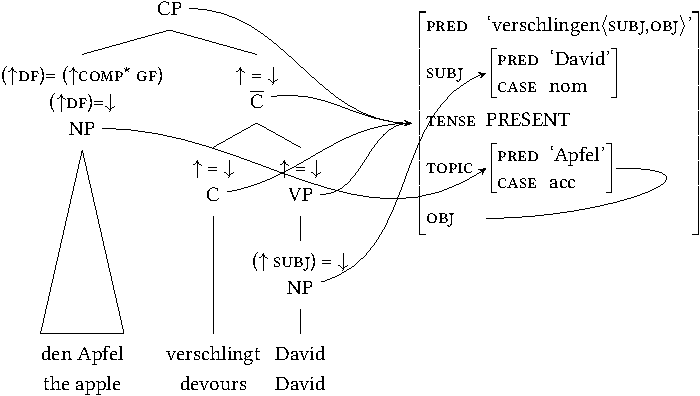
\includegraphics{Figures/den-apfel-verschlingt-david-lfg-lsp-crop}
}
\caption{\label{Abbildung-V2-LFG}Analysis of verb second}
\end{figure}%
\end{enumerate}

\section{Categorial Grammar}

\begin{enumerate}
\item The analysis of \emph{The children in the room laugh loudly.} is given in Figure~\ref{Abbildung-CG-Kinder-lachen-laut}.
\begin{figure}[H]
\centerline{%
\deriv{7}{
the   & children  & in  & the      & room                 & laugh & loudly\\
\hr   & \hr       & \hr & \hr      & \hr                    & \hr     & \hr \\
%
%
np/n  & n       & (n\bs n)/np & np/n & n                & s\bs np  & (s\bs np)\bs (s\bs np)\\
      &         &             & \multicolumn{2}{c}{\forwardapp} & \multicolumn{2}{c@{}}{\backwardapp}\\
      &         &             & np\\
      &         & \multicolumn{3}{c}{\forwardapp}  & \multicolumn{2}{c@{}}{s\bs np}\\
%
%
      &         & \multicolumn{3}{c}{n\bs n} \\  
      & \multicolumn{4}{c}{\backwardapp}\\
      & \multicolumn{4}{c}{{{n}}}\\
%
\multicolumn{5}{@{}c}{\forwardapp}\\
\multicolumn{5}{@{}c}{{np}}\\
%
\multicolumn{7}{@{}c@{}}{\backwardapp}\\
\multicolumn{7}{@{}c@{}}{{s}}\\
}}
\caption{\label{Abbildung-CG-Kinder-lachen-laut}Categorial Grammar analysis of \emph{The children in
    the room laugh loudly.}}
\end{figure}%

\item The analysis of \emph{the picture of Mary} is given in
  Figure~\vref{Abbildung-CG-das-Bild-von-Maria}. n/pp corresponds to \nnull, n corresponds to \nbar
  and np corresponds to NP.
\begin{figure}[H]
\centerline{%
\deriv{4}{
the & picture & of & Mary\\
\hr   & \hr     & \hr        & \hr\\
np/n  & n/pp    & pp/np      & np\\
%
      &         & \multicolumn{2}{c@{}}{\forwardapp}\\
      &         & \multicolumn{2}{c@{}}{pp}\\
%
      & \multicolumn{3}{c@{}}{\forwardapp}\\
      & \multicolumn{3}{c@{}}{n}\\
%
\multicolumn{4}{@{}c@{}}{\forwardapp}\\
\multicolumn{4}{@{}c@{}}{np}\\
}}
\caption{Categorial Grammar analysis of \emph{the picture of Mary}\label{Abbildung-CG-das-Bild-von-Maria}}
\end{figure}%
\end{enumerate}

\section{Head-Driven Phrase Structure Grammar}

\begin{enumerate}
\item The solution is \vpageref{avm-max-lacht}.
\begin{figure}
\oneline{%
\onems[head-argument-phrase~]{
      phon  \phonliste{ Max lacht }\\
      synsem$|$loc \ms{ cat \ms{ head & \ibox{1}\\
                                 subcat & \ibox{2} \eliste \\
                               }\\
                        cont \ms{ ind & \ibox{3}  \\
                                       rels & \relliste{ \ibox{4}, \ibox{5} } \\
                                     }\\
                      }\\
      head-dtr \onems[word]{ phon \phonliste{ lacht }\\
                             synsem$|$loc  \ms{ cat & \ms{ head   & \ibox{1} \ms[verb]{ initial & $-$\\
                                                                                        vform   & fin \\
                                                                                   }\\
                                                            subcat & \ibox{2}  $\oplus$ \sliste{ \ibox{6} }  \\
                                                        }\\
                                                 cont & \ms{ ind & \ibox{3} event \\
                                                                  rels & \liste{ \ibox{4} \ms[lachen]{ event & \ibox{3} \\
                                                                                                       agens & \ibox{7} \\ }} \\
                                                                }
                                               }\\
                       } \\
      non-head-dtrs \liste{ \onems[word]{ 
                                        phon \phonliste{ Max }\\
                                        synsem \ibox{6} \onems{ loc \ms{ cat & \ms{ head   & \ms[noun]{ cas & nom\\
                                                                                                      } \\
                                                                                    subcat &  \eliste \\
                                                                                }\\
                                                                         cont & \ms{ ind & \ibox{7} \ms{ per & 3 \\
                                                                                                              num & sg \\
                                                                                                              gen & mas \\
                                                                                                            } \\
                                                                                          rels & \liste{
                                                                                                  \ibox{5} \ms[named]{ name & max    \\
                                                                                                                       inst & \ibox{7} \\ }} \\
                                                                                         } \\
                                                                        }\\
                                                              }\\
                                   } 
                           } \\
}}
\label{avm-max-lacht}
\end{figure}%
\item An analysis of the difference in (\mex{1}) has to capture the fact that the case of the adjective has to agree with that of the noun. In (\mex{1}a),
the genitive form of \emph{interessant} `interesting' is used, whereas (\mex{1}b) contains a form that is incompatible with the genitive singular.
\eal
\ex[]{
\gll eines interessanten Mannes\\ 
     one.\gen{} interesting.\gen{} man.\gen{}\\
}
\ex[*]{ 
\gll eines interessanter Mannes\\
     one.\gen{} interesting.\nom{} man.\gen{}\\
}
\zl
(\mex{1}) shows the \catv of \emph{interessanten}.

\eas
\catv of \emph{interessanten} `interesting' with case information:\\
\ms{ head & \ms[adj]{ %prd & $-$ \\
                      mod  & {\upshape \nbar[\textsc{case} \ibox{1}]}\\
                      case & \ibox{1} gen\\
                    } \\
              subcat & \liste{} \\
}
\zs
The structure sharing of the case value of the adjective with the case value of the \nbar under \textsc{mod}
identifies the case values of the noun and the adjective. \emph{interessanten} can therefore be combined with 
\emph{Mannes}, but not with \emph{Mann}. Similarly, \emph{interessanter}
can only be combined with the nominative \emph{Mann}, but not with the genitive \emph{Mannes}. 

For a refinement of the analysis of agreement inside the noun phrase, see \citew[Abschnitt~13.2]{MuellerLehrbuch1}.
\end{enumerate}


\section{Construction Grammar}

Idioms can be found by reading the newspaper carefully. The less exciting method is to look them up a dictionary of
idioms such as the Free Dictionary of Idioms and Phrases\footnote{
\url{http://idioms.thefreedictionary.com/}, 04.03.2015.
}.


\section{Dependency Grammar}

\begin{figure}[H]
\centering
\scalebox{.9}{%
\begin{forest}
dg edges
[V
  [N [ich;I]]
  [habe;have]
  [N,name=n
    [Det,tier=det [einen;a]]
    [Mann;man]]
  [V [getroffen;met]]
  [Rel,no edge, tier=det,name=rel [\trace]
      [V
        [N [der;who]]
        [N [Adj, dg adjunct [blonde;blond]]
           [Haare;hair]]
        [hat;has]]]]
\draw (n.south)--(rel.north)-- +(0,6pt);
\end{forest}
}
\end{figure}%

\begin{figure}[H]
\centering
\scalebox{.9}{%
\begin{forest}
dg edges
[V
  [Subjunction
    [dass;that]
    [V, l sep+=15pt
      [N [er;he]]
      [Adv, dg adjunct [morgen;tomorrow]]
      [V [kommen;come]]
      [wird;will]]]
  [freut;pleases]
  [N [uns;us]]]
\end{forest}
}
\end{figure}%

\begin{figure}[H]
\centering
\scalebox{.9}{
\begin{forest}
dg edges
[V
  [V [N,name=n
       [Det,tier=det [einen;a]]
       [Mann;man]]
    [getroffen;met]]
  [Rel,no edge, tier=det,name=rel [\trace]
      [V
        [N [der;who]]
        [N [Adj, dg adjunct [blonde;blond]]
           [Haare;hair]]
        [hat;has]]]
  [habe;have]
  [N [ich;I]]
  [Adv [noch;yet]]
  [Adv [nie;never]]]
\draw (n.south)--(rel.north)-- +(0,6pt);
\end{forest}
}
\end{figure}%






\section{Tree Adjoining Grammar}

The elementary trees in Figure~\vref{TAG-Elementarbaeume-dem-Koenig-treue} are needed for the analysis of (\mex{1}).
\ea
\gll der        dem        König treue Diener\\
     the.\nom{} the.\dat{} king  loyal servant\\
\glt `the servant loyal to the king'
\z

\begin{figure}
\hfill
\scalebox{.9}{
\begin{forest}
tag
[Det [der;the]]
\end{forest}
}
\hfill
\scalebox{.9}{
\begin{forest}
tag
[Det [dem;the]]
\end{forest}
}
\hfill
\scalebox{.9}{
\begin{forest}
tag
[NP
  [Det$\downarrow$]
  [N$'$
    [N [König;king]]]]
\end{forest}
}
%
\hfill
%
\scalebox{.9}{
\begin{forest}
tag
[N$'$
  [AP
    [A$'$
      [NP$\downarrow$]
      [A [treue;loyal]]]]
  [N$'$*]]
\end{forest}
}
%
\hfill
%
\scalebox{.9}{
\begin{forest}
tag
[NP
  [Det$\downarrow$]
  [N$'$
    [N [Diener;servant]]]]
\end{forest}
}
\hfill\mbox{}
\caption{\label{TAG-Elementarbaeume-dem-Koenig-treue}Elementary trees for \emph{der dem König treue Diener}}
\end{figure}%

\noindent
By substituting the tree for \emph{dem} `the' in the substitution node of \emph{König} `king', one then arrives at a full NP.
This can then be inserted into the substitution node of \emph{treue} `loyal'. Similarly, the tree
for \emph{der} `the' can be combined with the one for \emph{Diener}. One then has both of the trees in Figure~\vref{TAG-substituiert}.

\begin{figure}
\hfill
\scalebox{.9}{
\begin{forest}
tag
[N$'$
  [AP
    [A$'$
      [NP
        [Det [dem;the]]
        [N$'$
          [N [König;king]]]]
      [A [treue;loyal]]]]
  [N$'$*]]
\end{forest}
}
%
\hfill
\scalebox{.9}{
\begin{forest}
tag
  [NP
     [Det [der;the]]
     [N$'$
        [N [Diener;servant]]]]
\end{forest}
}
\hfill\mbox{}
\caption{\label{TAG-substituiert}Trees for \emph{der dem König treue} and \emph{der Diener} after substitution}
\end{figure}%
The adjective tree can then be adjoined to the N$'$"=node of \emph{der Diener}, which yields the structure in Figure~\vref{TAG-Baeume-nach-Adjunktion}.
\begin{figure}
\centering
%\scalebox{.9}{
\begin{forest}
tag
  [NP
     [Det [der;the]]
     [N$'$
       [AP
         [A$'$
           [NP
             [Det [dem;the]]
             [N$'$
               [N [König;king]]]]
           [A [treue;loyal]]]]
       [N$'$
         [N [Diener;servant]]]]]
\end{forest}
%}
\caption{\label{TAG-Baeume-nach-Adjunktion}Result of adjunction of the AP to the N$'$"=node}
\end{figure}%




%      <!-- Local IspellDict: en_US-w_accents -->


\backmatter
\bookmarksetup{startatroot}

\bibliography{bib-abbr,biblio,lfg-implementations,temp}
\clearpage

\small
   

\phantomsection%this allows hyperlink in ToC to work
\addcontentsline{toc}{chapter}{Index} 
\addcontentsline{toc}{section}{Name index}
\ohead{Name index}
%with biblatex
%\printindex
%without it 
\printindex 
  
\phantomsection%this allows hyperlink in ToC to work
\addcontentsline{toc}{section}{Language index}
\ohead{Language index} 
\printindex[lan] 
  
\phantomsection%this allows hyperlink in ToC to work
\addcontentsline{toc}{section}{Subject index}
\ohead{Subject index}
\printindex[sbj]

\end{document}
